% The Chain Theory compendium. Build: ./build.sh (the whole compendium, then one PDF per Part cut from it).
\RequirePackage{fix-cm}  % lets the title page use Computer Modern at any size
\documentclass[11pt]{article}
\DeclareUnicodeCharacter{00D7}{\ensuremath{\mathchar"2202}}
\DeclareUnicodeCharacter{2124}{\ensuremath{\mathbb{Z}}}
\DeclareUnicodeCharacter{2086}{\textsubscript{6}}
\DeclareUnicodeCharacter{03B1}{\ensuremath{\alpha}}
\usepackage[margin=1in,headheight=14pt]{geometry}
\usepackage{fancyhdr}  % the running header carries the working-draft mark on every page
\pagestyle{fancy}
\fancyhf{}
\fancyhead[L]{\footnotesize\textsc{Chain Theory}}
\fancyhead[R]{\footnotesize\textsc{Working Draft}}
\fancyfoot[C]{\thepage}
\renewcommand{\headrulewidth}{0pt}
\fancypagestyle{plain}{\fancyhf{}\fancyhead[L]{\footnotesize\textsc{Chain Theory}}\fancyhead[R]{\footnotesize\textsc{Working Draft}}\fancyfoot[C]{\thepage}\renewcommand{\headrulewidth}{0pt}}
\usepackage{amsmath,amssymb,amsthm}
\usepackage{booktabs}
\usepackage{longtable}
\usepackage{cite}  % sorts and compresses the numbers inside each citation
\usepackage[colorlinks=true,linkcolor=blue,citecolor=blue,urlcolor=blue]{hyperref}
\newtheorem{theorem}{Theorem}
\newtheorem{definition}{Definition}
\newcommand{\rosetta}[2]{\emph{#1} (#2)}
\newcommand{\modref}[1]{Section~\ref{mod:#1}}
\newcommand{\rowcite}[1]{}
\setcounter{tocdepth}{1}
\title{Chain Theory: Toward Fundamental Physics from Distilling Networks of Entangled Qudits}
\author{A. D. Wissner-Gross\\\href{mailto:alexwg@alexwg.org}{\texttt{alexwg@alexwg.org}} \quad \url{https://www.alexwg.org}}
\date{}
\usepackage{amsthm}
\usepackage{framed}
\usepackage{xcolor}
\usepackage{etoolbox}
\theoremstyle{plain}
\newtheorem{chtheorem}{Theorem}[section]
\newtheorem{chconditional}[chtheorem]{Theorem}
\newtheorem{chwall}[chtheorem]{Open result}
\newtheorem{chdefinition}[chtheorem]{Definition}
\newtheorem{chtable}[chtheorem]{Table}
\newenvironment{chbox}[1]{\def\FrameCommand{\setlength{\fboxsep}{4pt}\setlength{\fboxrule}{.4pt}\fcolorbox{black}{#1}}\MakeFramed{\advance\hsize-\width\FrameRestore}}{\endMakeFramed}
\BeforeBeginEnvironment{chtheorem}{\begin{chbox}{black!6}}\AfterEndEnvironment{chtheorem}{\end{chbox}}
\BeforeBeginEnvironment{chconditional}{\begin{chbox}{black!6}}\AfterEndEnvironment{chconditional}{\end{chbox}}
\BeforeBeginEnvironment{chwall}{\begin{chbox}{black!10}}\AfterEndEnvironment{chwall}{\end{chbox}}
\BeforeBeginEnvironment{chdefinition}{\begin{chbox}{black!3}}\AfterEndEnvironment{chdefinition}{\end{chbox}}
\BeforeBeginEnvironment{chtable}{\begin{chbox}{black!3}}\AfterEndEnvironment{chtable}{\end{chbox}}
\newenvironment{chproof}[1][]{\begin{proof}[Derivation\ifx&#1&\else\ (#1)\fi]}{\end{proof}}
\newenvironment{chbridge}{\par\medskip\noindent\textit{In the language of the literature.}\ }{\par\medskip}
\newcommand{\chstanding}[1]{\par\noindent{\footnotesize\textit{Standing:} #1.}\par}
\newcommand{\chdeps}[2]{\par\noindent{\footnotesize\textit{From} \ifblank{#1}{---}{#1.} \textit{Used by} \ifblank{#2}{---}{#2.}}\par}
\makeatletter
% three-digit section numbers in the contents need a wider number box than article's 1.5em
\patchcmd{\l@section}{\setlength\@tempdima{1.5em}}{\setlength\@tempdima{2.3em}}{}{\PackageWarning{preamble}{l@section not patched}}
\newcommand{\chdesig}[4]{\par\noindent{\footnotesize\textsf{Chapter #1}\def\ch@x{#2}\ifx\ch@x\@empty\else, \textsf{#2} in the module numbering\fi\def\ch@a{#3}\def\ch@b{#4}\ifx\ch@a\ch@b\else{} \textit{(sections \ref{mod:#3} to \ref{mod:#4})}\fi}\par\smallskip}
\makeatother
\newcommand{\chinstrument}[2]{\par\noindent{\footnotesize\textit{Instrument chapter of Part #1.}}\par}
\newcommand{\chcert}[1]{\par\noindent\textit{Certified at the repository; #1 objects enumerated.}\par}
\usepackage{graphicx}
\usepackage{tikz}
\usepackage{adjustbox}  % wide tables, pictures and equations shrink to the line instead of running into the margin
\setlength{\emergencystretch}{3em}
\usepackage{float}

% Generated by compendium/tools/index.py from the boxed statements; do not edit by hand.
\newcommand{\atlasTheorems}{100}
\newcommand{\atlasConditionals}{109}
\newcommand{\atlasOpen}{198}
\newcommand{\atlasTheoremsLean}{64}
% The rows of Table 237.1: Part, theorems, of them tied to Lean, conditional theorems, open results, tables, definitions.
\newcommand{\atlasByPartRows}{%
I & 20 & 17 & 9 & 23 & 4 & 6 \\
II & 0 & 0 & 0 & 0 & 1 & 0 \\
III & 1 & 0 & 8 & 4 & 1 & 0 \\
IV & 6 & 3 & 5 & 4 & 1 & 0 \\
V & 14 & 8 & 6 & 24 & 2 & 0 \\
VI & 2 & 0 & 17 & 30 & 2 & 0 \\
VII & 5 & 1 & 10 & 9 & 3 & 0 \\
VIII & 1 & 1 & 8 & 17 & 1 & 0 \\
IX & 1 & 1 & 12 & 12 & 1 & 0 \\
X & 6 & 2 & 18 & 8 & 2 & 0 \\
XI & 2 & 1 & 3 & 2 & 0 & 0 \\
XII & 1 & 1 & 9 & 16 & 2 & 0 \\
XIII & 7 & 7 & 0 & 5 & 1 & 0 \\
XIV & 6 & 6 & 0 & 3 & 1 & 0 \\
XV & 11 & 11 & 1 & 5 & 0 & 0 \\
XVI & 0 & 0 & 0 & 0 & 4 & 0 \\
appendices & 6 & 3 & 2 & 23 & 0 & 0 \\
instruments & 11 & 2 & 1 & 13 & 28 & 1 \\
\hline
all & 100 & 64 & 109 & 198 & 54 & 7 \\}
  % the release counts, generated by tools/index.py
\begin{document}
\thispagestyle{empty}
\null\vfill
\begin{center}
{\fontsize{44}{52}\selectfont Chain Theory\par}
\vspace{1.4em}
{\Large Toward Fundamental Physics from Distilling\\[0.3em] Networks of Entangled Qudits\par}
\vspace{2.6em}
{\Large\itshape A Compendium of Preliminary Findings\par}
\vspace{1.6em}
{\large\bfseries WORKING DRAFT\par}
\vspace{3.4em}
{\large A. D. Wissner-Gross\par}
\vspace{0.8em}
\href{mailto:alexwg@alexwg.org}{\texttt{alexwg@alexwg.org}} \quad \url{https://www.alexwg.org}\par
\vspace{1.6em}
{\large October 23, 2026\par}
\end{center}
\vfill\null
\clearpage
\section*{Preface}\label{front:preface}
In the first three decades of the twentieth century, fundamental physics was rebuilt from its foundations. Between Planck's quantum of 1900 and Dirac's equation of 1928 came special relativity, general relativity, the quantum theory of the atom, and quantum mechanics itself, each a new framework and most of them confirmed within a few years. The decades that followed turned those frameworks into the Standard Model, whose structure was considered complete by the middle of the 1970s.

Since then, fundamental physics has been starved of new structure. The great experiments of the last fifty years, the W and Z bosons (1983), the top quark (1995), the Higgs boson (2012), and gravitational waves (2015), confirmed predictions made decades earlier. The genuine surprises of 1998, neutrino masses and the accelerating expansion of the universe, were found by experiment, explained by no theory, and added free parameters to a count that was meant to shrink. The drought is now longer than the golden age it followed. A drought that long is a sign that what is missing is not more data but a different starting point.

However, the field of physics drew a different conclusion. For most of the twentieth century, the aim of fundamental physics was derivation, fewer inputs and more outputs, and the constants of nature were the outputs still owed. The Standard Model settled the structure but not the numbers. Its two dozen or so parameters are measured, not derived, and nothing within it explains their values. As the drought set in, the aim itself changed. One line of argument concluded that the constants are not derivable from law at all, that their observed values are environmental, selected by the condition that observers exist. Its one notable success was Weinberg's anthropic bound (1987) on the cosmological constant, which pointed to a small nonzero value a decade before the accelerating expansion was measured.

The string landscape then supplied a vast population of vacua to select from, and its predictions came to rest on the assumption that we are typical observers within it, a Copernican principle stretched across universes. What counts as typical depends on a measure over infinitely many regions, and no one has fixed that measure. A large part of the field moved from deriving the constants to explaining why they could not be derived. The swampland program is a partial return. It asks which effective theories are consistent with quantum gravity at all, but it asks largely from within string theory and leaves the constants where the landscape put them. In retreating, the field kept its foundations and gave up on derivation. The opposite course is to hold derivation as the goal and look for new foundations.

The clues to those foundations may have been in plain sight all along. A derivation with no free parameters, and no appeal after the fact to the existence of observers, may need no new experiment to begin. Three clues in the existing body of physics already point the way. Each has been interpreted as something else: a bound as a fact about black holes, a gauge group as a blemish to be embedded, and a null result as a scale not yet reached.

The first clue is that the information a bounded region of space can hold is finite. This bound was first derived by Jacob Bekenstein (1981) from black hole thermodynamics and is usually regarded as a fact about gravity, but it constrains whatever fills the region, elementary matter included. Gravitational dynamics has since been derived from the entanglement of such regions, beginning with Ted Jacobson (1995). The lesson for elementary matter is direct. A field has infinitely many degrees of freedom in every region, and a string has infinitely many modes of vibration. A finite bound says to look instead for finitely many degrees of freedom, carried by quantum systems of finite dimension.

The second clue is the Standard Model gauge group, interpreted as a signature and not a blemish. Grand unification treated the product $\mathrm{SU}(3)\times\mathrm{SU}(2)\times\mathrm{U}(1)$ as an ugliness to be embedded in a simple group: SU(5) in the model of Georgi and Glashow in 1974, then SO(10), E$_6$, and supersymmetric versions of each. It paid for the embedding with predictions that have not appeared: no proton has been seen to decay, and no supersymmetric partner of any known particle has turned up at any collider. However, the same apparently ugly product can instead be understood as the symmetry of a single object of a different kind: a qutrit and a qubit sharing one entangled state. Changes of basis at the two ends contribute SU(3) and SU(2), and of their two phases only one survives, belonging to neither end but to the pair. These local transformations form the Standard Model gauge group, including the $\mathbb{Z}_6$ quotient that its observed charges permit.

The third clue is that the elementary particles of the Standard Model have shown no substructure. Over decades, every one of them has behaved as a point. Colliders have raised, by orders of magnitude, the energy up to which the electron and the quarks show no substructure, and searches for the excited states and contact interactions that constituents would produce in scattering have returned nothing. Yet the particle spectrum itself, three generations repeating one set of charges, is the kind of pattern that has always signaled constituents, from the periodic table to the hadrons, and compositeness has been set aside chiefly because no constituents appear. There is, however, another interpretation. Suppose nature is saying not that the substructure is hard to resolve but that it cannot be resolved at all. Quantum information knows one kind of correlation with exactly that property. A state of two systems can be entangled, certifiably so, and yet admit no procedure by local operations and classical communication that distills, from any number of its copies, a single maximally entangled pair, or anything close to one. Such entanglement was identified in 1998 by Micha{\l}, Pawe{\l}, and Ryszard Horodecki, who called it ``bound.'' It cannot be extracted or directly observed, but it can be detected indirectly. An entanglement witness, a measurement tailored to the state, can certify that it is there. If the constituents of an elementary particle were joined by entanglement that the available operations cannot extract, scattering, which looks for constituents by resolving them, would find nothing to resolve and would see a point, while a suitable witness could still show that the structure exists. The substructure of elementary matter, on this interpretation, would not be undetectable. It would be undistillable.

Put together, the clues hint at a single new foundational theory. The first suggests that everything consists of finitely many quantum systems, each of finite dimension, so that every degree of freedom is discrete. The second suggests that these systems, or qudits, come in entangled pairs, and the first clue fixes how strongly: a pair entangled any less than maximally would carry continuous parameters, its Schmidt coefficients, that a theory without continuous degrees of freedom cannot afford. The third suggests that an elementary particle is built from many such pairs, and with nothing but pairs to build from, the only way to join them is for pairs to share a qudit, so the pairs form a network. Monogamy of entanglement forbids any one system from being maximally entangled with two partners, so a shared qudit cannot be a single system sitting in two pairs. It holds instead one copy of itself for each of its pairs, and each pair is maximally entangled with its own copy, much as a four-dimensional system, which has room for two qubits, can be maximally entangled with two separate qubits at once. The shared qudit is the join where those copies meet and their bases are matched, just as the bonds of a projected entangled pair state (PEPS), a standard kind of tensor network, meet at a site. The third clue also divides the network. The links we observe directly can each be fixed by a single distillation. The links inside an elementary particle are just as maximally entangled, but no single distillation fixes them, which is the theory's analogue of bound entanglement and the reason every particle looks like a point. An elementary particle, in this picture, is a finite ``chainmail'' whose links are such pairs.

Chain Theory is an emerging research program of mine that treats this chainmail as all there is. It takes literally John Wheeler's 1989 proposal, ``it from bit,'' with finite quantum systems in place of bits, and its single axiom gathers the three clues into eighteen words: \textbf{``Nothing exists but finitely many maximally entangled pairs of finite-dimensional systems, some shared, known only by distilling them.''} To distill, in the axiom, means to join two systems into a perfectly entangled pair in a single step. It is the same move that passes entanglement along a quantum network, and it means there is no observer outside the network: to learn about a link is to link to it. In a laboratory this step succeeds only part of the time, but in the theory it is the only thing that ever happens.

It already appears that many elements of fundamental physics, including parts of both the Standard Model and general relativity, follow from that axiom. The sharpest test is a number. The fine-structure constant in the Thomson limit, $\alpha(0)$, is one of the most precisely measured numbers in all of science, known to about one part in ten billion, yet the Standard Model takes it from experiment. Richard Feynman wrote that ``all good theoretical physicists put this number up on their wall and worry about it,'' and called it ``a magic number that comes to us with no understanding by man.'' It is also a number with no visible pattern. A simple value such as the 2/3 of Koide's relation among the lepton masses can be reached by many short formulas, but ten digits of a number like $\alpha(0)$ are far harder to match by accident. Because the Standard Model takes $\alpha(0)$ from experiment, a derivation of it would, almost by definition, draw on physics beyond the Standard Model, and ten measured digits could make $\alpha(0)$ an exquisite probe of that physics. Chain Theory yields an exact candidate for it, the algebraic number $(79 + 48\sqrt{2} + 42\sqrt{3} + 3\sqrt{6})/31104$, a weighted count over the 172 measurement records of a single entangled pair, small enough to check by hand. The pair is a qutrit maximally entangled with a qubit, the same object whose changes of basis give the Standard Model gauge group, and I conjecture that this pair is the link from which photons are built, which would make the number $\alpha(0)$. Its inverse is $137.035\,999\,189\,566\ldots$.

The standard reference value for $\alpha(0)$ comes from CODATA, the international committee that every four years combines the world's most precise measurements into one recommended value for each fundamental constant. Its 2022 recommendation for the inverse is $137.035\,999\,177$, with a standard deviation of 21 in the last two digits. The Chain Theory-derived number agrees with the CODATA recommendation in its first ten significant digits and lies 0.60 standard deviations from it, between the two most precise determinations. The experimental measurements still disagree with one another by more than their stated uncertainties, so this comparison is not yet decisive. But the number is now fixed, and new measurements of the electron's magnetic moment at Northwestern University and of atomic recoil in Berkeley and Paris aim to be up to ten times more precise. If they agree with one another, they will either close in on the derived value or rule it out.

Beyond $\alpha(0)$, preliminary Chain Theory results range from quantum foundations to cosmology: the Standard Model gauge group as a theorem, and the Born rule, the Lorentz group and the signature of spacetime, three generations of matter, confinement, curvature, and the cosmological term as derivations whose remaining conditions are named in each case. Other programs have derived parts of the Standard Model from finite or algebraic inputs, among them braided ribbons, an exceptional Lie group, the division algebras, and noncommutative geometry, but none supplies the value of a coupling constant to within experimental precision. Closed-form expressions for the fine-structure constant, meanwhile, have a long and mostly numerological history. Mine differs in the one respect that matters: the number is a theorem of a stated axiom, its definitions and a few stated readings of them, checked in Lean rather than fitted, and only its identification with $\alpha(0)$ is conjectured.

The Chain Theory axiom's last clause also says which links can be observed directly, the question the third clue raised. The links of the chainmail network come in types labeled by the dimensions of their two ends, and the theory identifies each type with a sector of physics: (2,2) with spacetime, (3,2) with electromagnetism, (3,3) with the strong interaction, (4,2) with the weak interaction, (4,3) with the Yukawa sector, and (4,4) with the Higgs. Read at the level of these types, the axiom's last clause says that two ends are known only when every consistent relation between them is one that distillation can carry. Classic theorems from the 1960s and 1970s by St{\o}rmer, Woronowicz, and Choi show that this holds exactly when the two dimensions multiply to at most six, the same threshold beyond which bound entanglement becomes possible. So only spacetime and electromagnetism can be observed directly by distillation. The other four types are ``dark'': their links are just as maximally entangled, but their ends are related in ways no distillation carries, so they are observed only at second order, through two distillations, which the theory identifies at (3,3) with confinement.

I call this theory ``Chain Theory'' for three reasons. The first is to draw a contrast with string theory: an elementary particle is a finite chainmail of discrete links, not a continuous string. The second is how the links join. Pairs meet at shared qudits, and each join carries a gauge freedom in how bases are matched across it, much as two links of a physical chain can turn against each other at their join without changing the chain. The third is direction. A distillation passes its basis outward along each link to the far end, so what is known accumulates in a fixed order, each distillation building on those before it, the way a chained ledger grows by linking each new entry to the last.

The last golden age rebuilt physics from its foundations in three decades. I do not yet claim to have done the same. Chain Theory is new, much of it is still conditional or underdeveloped, and it will benefit from the contributions of many others. But if the clues have been interpreted correctly, the foundations for another golden age, built this time from quantum information, may already be in hand, and what remains is to find out how much of physics they can carry.

\begin{flushright}\textit{A. D. Wissner-Gross, Cambridge, Massachusetts, October 2026}\end{flushright}

\clearpage
\tableofcontents
\clearpage
\begin{abstract}\label{front:abstract}
Chain Theory is an emerging program to study fundamental physics through the lens of quantum information. In the spirit of Wheeler’s ‘it from bit,’ its single axiom says that nothing exists but finitely many maximally entangled pairs of finite-dimensional systems, some shared, known only by distilling them. This compendium collects some of the program’s preliminary findings to date, each stated in standard form beside its derivation and graded as a theorem, a conditional theorem, or an open result. From the axiom we obtain, as conditional theorems, the state space, the Born rule, unitarity, the uncertainty relation, the rotation and Lorentz groups, the signature of spacetime, and parity, time reversal, and CPT, and, as a theorem, conservation laws. We identify correspondences between (M,N) links of finite M- and N-dimensional systems with: spacetime for (2,2), electromagnetism for (3,2), the strong interaction for (3,3), the weak interaction for (4,2), the Yukawa sector for (4,3), and the Higgs for (4,4). We obtain the gauge group SU(3) × SU(2) × U(1) and the second law as theorems; as conditional theorems, an exact algebraic number conjectured to be the Thomson-limit fine-structure constant within 0.60 sigma of its measured value, the electron anomalous moment through third order, the hydrogen spectrum, parity violation, confinement, the running of the couplings, decay rates as finite sums with no renormalization, curvature, and the cosmological term; and, partly as conditional theorems and partly as open results, three generations, masses, and anatomies of the Standard Model particles. Beyond the Standard Model, the same construction yields, as theorems, band structure and the Chern number, phase transitions, and a distillation theorem for quantum computation. This release holds \atlasTheorems{} theorems, \atlasConditionals{} conditional theorems and \atlasOpen{} open results; \atlasTheoremsLean{} of the \atlasTheorems{} theorems are tied to named Lean declarations, which check the finite computations their derivations use.
\end{abstract}
\section*{Introduction}\label{sec:intro}\label{front:introduction}
This compendium derives from one sentence and six definitions a web of theorems and open results connecting quantum information to fundamental physics, the Standard Model and gravity among them. The sentence says that the world is a finite collection of maximally entangled pairs of finite quantum systems, that some of those systems are shared between pairs, and that the only way anything is learned about them is by distilling them. Its six definitions, printed word for word in the framework chapter and again at chapter 1-1, are the whole of the theory. The compendium is the product of a long-term human-superintelligence collaboration to work out their consequences across physics, from quantum foundations and particle physics to gravitation, condensed matter and quantum computation. Every result the compendium prints is a theorem, a theorem conditional on a premise named beside it, an open result carried to a named step, a presentation, or a dissolved word, and the status of every claim is printed beside it. Every term of the theory that the chapters use, from the act and the read to the web, the sink and the wash, is defined in the glossary that follows this introduction. The first result of the program is the exact number of the alpha Letter, \emph{A Parameter-Free Candidate for the Fine-Structure Constant from Entangled Qudits}, whose computation the Letter's Lean file checks in full and which the Letter conjectures to be the fine-structure constant $\alpha(0)$. Chapter 7-1 of Part VII gives an earlier form of the same computation; where the two differ, the Letter is the canonical statement.

\paragraph{The modular form.} This release of the compendium has sixteen Parts of 116 chapters, with two chapters of the first Part at appendix slots, every chapter self-contained at the one shape the framework chapter describes, and the map of every chapter at the page that follows this introduction. The sixteen Parts are the framework (Part I), the rule, the chain automata and the single root (Part II), quantum mechanics (Part III), spacetime, symmetry and the dynamics of the read (Part IV), the matrix, the Standard Model at the six genres (Part V), the metric, the worldline and the horizon (Part VI), the photon (Part VII), the carriers and the breaking (Part VIII), the junction (Part IX), the Yukawa leg and the Higgs offices at the bodies (Part X), the Higgs, its hub register and the dressing field (Part XI), decays and nuclear physics (Part XII), thermodynamics (Part XIII), condensed matter and atoms (Part XIV), quantum information (Part XV), the scorecard, the open results and what remains (Part XVI). Every result is placed at one chapter, the instrument chapters of every Part are printed among the instruments at the end of this compendium, with one listing chapter per Part, and a result whose derivation is not yet written stands at one line of the results table of the last Part at its title, its standing and its citation.

\paragraph{The shape of a chapter.} Every chapter has one shape, set out in the framework chapter: the known result, the textbook statement in standard notation with its citation; the statement of the theory, with the results it rests on; the derivation in brief, every theorem restated at the union of the conditions of its own ancestors; the status and the number; and what stands open. Every term of the theory is defined once in the glossary that follows this introduction, with its nearest standard concept, so that a physicist reads every chapter in the standard vocabulary.

\paragraph{The status words.} The compendium grades every result at one of four statuses, and every chapter says the status of its results in words. A theorem is a statement derived from the axiom, the definitions and the results proved ahead of it; in this release \atlasTheoremsLean{} of the \atlasTheorems{} theorems are tied to named Lean declarations, which check the finite computations their derivations use; a theorem conditional on a premise prints the premise beside it, and under the chain rule of this compendium every theorem prints at its statement the union of the conditions of the results it rests on, a composed claim carrying the lowest status in its chain. An open result is a derivation carried to a named step, the first open cell located from two sides, neither established nor excluded, with the step named beside the claim. A presentation, such as a table, a tool, or this compendium itself, makes no claim of its own. A word is dissolved when the derivation has shown that no derived cell depends on it, so that the word is a presentation and not a fact. Beside these, a literature name is used by name and consumed as a premise never, and an observed value enters this compendium only as a display beside a derived figure with its provenance. Where the words admit two readings both are printed and none is selected. The only inputs not derived are the Axiom, its definitions, the premises printed beside the conditional theorems, and the conjectures, each marked as such.

\paragraph{Three clues.} The preface sets out the three clues in plain terms, and this paragraph gives their sources in the same order. The first is finiteness: the bound on the information of a bounded region \cite{Bekenstein1981}, which black hole thermodynamics first suggested \cite{Bekenstein1973}, and the derivations of gravitational dynamics from entanglement \cite{Jacobson1995,RyuTakayanagi2006,Jacobson2016}, in the lineage of Wheeler's proposal that physics is information at bottom \cite{Wheeler1990} and of the reconstructions of quantum theory from informational axioms \cite{Hardy2001,Chiribella2011}. The second is the gauge group, read as a signature and not a blemish. Grand unification embedded the product SU(3) x SU(2) x U(1) in a simple group \cite{GeorgiGlashow1974} and paid for the embedding with predictions that have not appeared; Chain Theory reads the same product as the description of one object, a pair of a qutrit and a qubit with SU(3) acting at one end, SU(2) at the other and a phase that neither end owns, the identification freedom the definitions leave at a link whose ends have dimensions two and three, and Part V derives the group as a corollary of one construction. The third is the null result of the searches for substructure, read as undistillability rather than distance: bound entanglement admits no procedure by local operations and classical communication that distills from any number of its copies a single maximally entangled pair \cite{Horodecki1998,Horodecki2009}, yet an entanglement witness certifies its presence \cite{Terhal2000}, the partial transpose being the first such test \cite{Peres1996}, and the related states that hide classical data from every local reader are the data-hiding states \cite{DiVincenzo2002}. The Axiom postulates the first clue exactly, finitely many pairs of finite systems and nothing continuous, and the first result of the program is that a constant follows once the finite objects are named.

\paragraph{Derivability as a method.} One research program concluded that the constants of nature are not derivable from law, the observed values being environmental \cite{Weinberg1987}; that is a coherent position and a change of question, and this compendium takes the opposite bet as a matter of method: the constants are theorems of a finite structure, and the compendium tries to compute them. The swampland program shares the derivability aim from within string theory \cite{Vafa2005}; the difference is where the finiteness is put, here at the start, in the Axiom, so that every quantity of the theory is a count or a trace over a finite register and there is nothing left to select from. Several published programs derive parts of the Standard Model from a finite or algebraic input, braided ribbons \cite{BilsonThompson2005}, one representation of an exceptional group \cite{Lisi2007}, the division algebras \cite{Furey2016} and the spectral action on a finite noncommutative geometry \cite{ChamseddineConnes1997}; here no unification group and no division algebra is an input, the only algebraic objects being the Weyl operators of finite-dimensional systems and the identification groups the definitions leave, and the construction supplies a coupling constant, which those programs do not. Closed-form expressions for the fine-structure constant have a long lineage \cite{Eddington1946}; the expression of this compendium differs in that it is a theorem of a stated axiom and not a fit.

\paragraph{The program and its name.} The premise our program reached is one sentence of eighteen words, a choice we made and not a derivation, printed word for word at the framework chapter. In plain terms, a qudit is a finite-dimensional quantum system; a qudit is shared when it is one end of two or more pairs; distilling is projecting two qudits onto a maximally entangled pair on their common support, which in standard language is entanglement swapping \cite{Zukowski1993}; a read is a distillation of a qudit with another in one of its bases, one read for each basis, giving the qudit its only basis and passing that basis along each pair to its far end; and what is known of a qudit is what all its reads, taken jointly, fix with certainty, whichever way the basis directions are matched across its pairs, with one further clause about two reads that commute only up to a sign. The name has three sources: the postulate that elementary particles are composed of finite chains of links rather than continuous strings; the object the definitions describe, a graph of pairs joined at shared qudits, each join carrying a gauge freedom in the identification of bases; and the direction of the record, every walk read in the read order from the site of the read to the far end.

\paragraph{The compendium and its Lean, the releases and the repository.} This compendium, its Lean packages and its index are published together in the repository \texttt{chain-theory} under the release tags \texttt{compendium-v*}; the alpha Letter is released separately under the tags \texttt{alpha-v*}. The compendium's README in the repository describes the reading paths and the build.
\section*{Glossary}\label{app:glossary}
The glossary gives, for every term of the theory that the compendium uses, its meaning in one sentence and its nearest standard term in another. The sentence on the nearest standard term says whether the standard object is the same object or only the nearest one, and says so when none is matched. The Rosetta table, printed in full as chapter~\ref{mod:I-7-rosetta-table-in-full} among the instruments, lines every noun of the theory with its nearest standard concept in the same way.
\begin{description}\setlength{\itemsep}{1pt}
\item[the act] The act is one distillation of two qudits. In standard terms it is exactly a Bell-basis projection of two qudits, an entanglement swap.
\item[the act outputs] The act outputs are the possible outcomes of one act, and their span is the state space. In standard terms they are exactly the outcomes of a projective measurement.
\item[the acting site] The acting site is the qudit at which the act of a read is applied, the site whose side fixes the slot of a second-order read at a cut. The nearest standard term is the vertex at which a measurement acts.
\item[the alpha letter] The alpha letter is the manuscript of the project that derives the fine-structure constant from the one link, issued in numbered releases. The nearest standard term is a paper on the fine-structure constant.
\item[the apparatus web] The apparatus web is the network of pairs that stands for the measuring instrument, joined to the body it reads. The nearest standard term is the measuring apparatus modelled as part of the quantum system.
\item[the arm] An arm is a link at a site. In standard terms it is exactly a half-edge of a graph at a vertex.
\item[the arrow] An arrow is a direction on a link. In standard terms it is exactly a directed edge.
\item[the attach count] The attach count is the number of attach sites a body carries. The nearest standard term is the number of interaction vertices of a diagram.
\item[the attach site] The attach site is the qudit at which one body is joined to another by a pairing. The nearest standard term is an interaction vertex.
\item[the attachment pair] The attachment pair is the pair through which a body is read. The nearest standard term is a coupling edge between two subsystems.
\item[the axiom sentence] The axiom sentence is the one sentence of the axiom, that nothing exists but finitely many pairs. The nearest standard term is the postulate of a theory stated in one sentence.
\item[the body] The body of a particle is its web, a network of pairs and not a state vector. The nearest standard term is the state of a particle.
\item[the body-alone rule] The body-alone rule reads the office of a body from the web of the body alone, the measuring apparatus adding nothing, so that the Born square at each of the five bodies is exact. The nearest standard term is the rule that an expectation value depends on the state of the system alone and not on the apparatus.
\item[the bond] The bond is the link that joins the electron body to the proton body in the hydrogen web, the link at which the two-vertex term is read. The nearest standard term is the binding of the electron to the proton in the hydrogen atom.
\item[the Born count] The Born count is the count of records at the full web, the dressed measure a readout is normalized by. The nearest standard term is the normalizing trace of the Born rule.
\item[the Born square] The Born square is the square of the read at the Born rule. In standard terms it is exactly the Born probability, the squared amplitude.
\item[the boundary count] The boundary count is the count of reads across an interface, a count and no entropy. The nearest standard term is the entanglement entropy across a cut.
\item[the bra end] The bra end is the bra end of a link in the copy model, where every link joins one ket end and one bra end. The nearest standard term is the bra index of a tensor factor.
\item[the cap] The cap is the depth at which a closure is read, the bound of a reading. The nearest standard term is a cutoff on the depth of an iteration.
\item[the cap algebra] The cap algebra is the algebra of the letters read at the depth cap, the Weyl algebra at the capped sinks. The nearest standard term is the operator algebra of a theory at a cutoff.
\item[the cap census] The cap census is the tally of the sinks reached at the depth cap, listed by their kind. The nearest standard term is a tally of the fixed points reached within a cutoff.
\item[the capped sink] The capped sink is a sink read at the depth cap, the closure stopped at its bound. The nearest standard term is a fixed point of a truncated iteration.
\item[the carrier] A carrier is the closed read of a readable genre; the boson is named by correspondence. The nearest standard term is a gauge boson, a force carrier.
\item[the Cartan word] The Cartan word names the functionals of the kernel that take the role of the weights of a Lie algebra, posed on the typed count and left open there. The nearest standard term is the Cartan subalgebra of a Lie algebra and its weights.
\item[the Clifford group] The Clifford group is the group of moves the reflections and the letters generate, named at the universality of the move set. The nearest standard term is the Clifford group of quantum computation.
\item[the closed leg] A closed leg is a link at a hub whose far end is traced over, its dimension entering the dressing of the read. The nearest standard term is a contracted index, an internal line of a diagram.
\item[the closed read] A closed read is a read whose basis returns to its start, the carrier at a readable genre. The nearest standard term is a closed walk of measurements, a loop.
\item[closure] The closure of a seed is its orbit under the moves, graded by waves. In standard terms it is exactly the forward closure of a set under operations.
\item[the common support] The common support of two qudits is the subspace on which a pair of them can be projected. In standard terms it is exactly the intersection of the supports of two projectors.
\item[the commutant] The commutant is the set of kernel functionals that commute with every move of the full move set, the conserved counts of the theory. The nearest standard term is the commutant of an operator algebra, the set of conserved charges.
\item[the comparison word] The comparison word is the word a board prints beside a computed figure and a tabulated one, saying how the two stand. The nearest standard term is the verdict of a comparison between a prediction and a measurement.
\item[the copy] A copy is one of the two indices a link joins, in the copy model every link joining one ket end and one bra end. In standard terms it is exactly a ket index or a bra index of a tensor.
\item[core] The core is the site the closure closes at, the one link of a body opened. The nearest standard term is the root vertex of a tree-shaped state.
\item[the count of a read] The count of a read is the number of records the read fixes, posed as the rank at the cut and left open there. The nearest standard term is the rank of a measurement projector.
\item[the cross core] A cross core is a core shared across two bodies at their join, its doublets counted at the joined web. The nearest standard term is an interaction vertex shared by two subsystems.
\item[the cut] The cut is the move that removes a link of a web, the reverse of the pairing. The nearest standard term is the removal of an edge from a graph.
\item[the cycle] A cycle is a closed path of links; an odd cycle carries the holonomy sign. In standard terms it is exactly a cycle of a graph.
\item[the dark genre] A dark genre is a genre whose link admits no read at the one link, the pair of two qutrits among them. The nearest standard term is a hidden sector, an unobservable sector.
\item[the dark link] A dark link is a link of a genre no read can pass, so that its records enter a readout only through their counts. The nearest standard term is an unobservable degree of freedom, an edge of a hidden sector.
\item[the dark set] The dark set is the set of the dark links of a web. The nearest standard term is the hidden sector of a theory.
\item[the decay board] The decay board is the table that lists the decay rates the compendium computes beside their comparison words. The nearest standard term is a table of decay widths and lifetimes.
\item[the decoupling] The decoupling is the register count below the cap, the part of a read that a body beyond the cap cannot move. The nearest standard term is the decoupling of heavy degrees of freedom below a scale.
\item[the delta] The delta is the change a move makes at a web, the records carried across it. The nearest standard term is the difference of two states under a map.
\item[the depth] The depth is the growth order of a closure, the count of waves to the horizon. The nearest standard term is the circuit depth, the number of rounds.
\item[distilling] Distilling is projecting any two qudits onto a pair on their common support, the one operation the axiom allows. The nearest standard term is a Bell-basis projection, an entanglement swap; the standard distillation of entanglement by local operations is a different object.
\item[dock] A dock is a link of two qubits whose far end is washed, the charge register of a body. The nearest standard term is a leaf pair at a terminal qubit, a dangling edge.
\item[the dressing] The dressing of a body is the far-end dimension of its hub legs, the Born product over the legs that multiplies the rank at the office. It is also called the hub dressing of a body, or the hub-leg Born product; no closer standard term is matched.
\item[the enclosed set] The enclosed set is the set of records a closed path of the web encloses, whose count is the wash integer of the fan loops. The nearest standard term is the flux enclosed by a loop.
\item[the exchange] An exchange is a swap a record survives; the count of exchanges grades the record sum. The nearest standard term is a swap of two subsystems, an exchange interaction.
\item[the face] A face is one of two readings of a word that the reads admit; both are printed beside each other and neither is selected. There is no standard term; the nearest description is one of two admissible interpretations of a read word.
\item[the far end] The far end of a pair at a qudit is the other qudit of that pair. In standard terms it is exactly the partner qudit of an entangled pair.
\item[the fine-structure star] The fine-structure star is a qutrit of degree three with three arms of the two-three genre, two read and one held. The nearest standard term is a graph state on a star of three edges.
\item[the finiteness word] The finiteness word is the clause of the axiom that the pairs are finitely many, carried as the axiom itself and struck from the formal statement where it had stood as a premise. The nearest standard term is a finiteness assumption of a theory.
\item[the first power] The first power is the sum of the act readouts of a web, the grading by exchanges at order one. The nearest standard term is the first-order term of the coupling expansion.
\item[the five bodies] The five bodies are the electron, the muon, the tau, the proton and the neutron webs of the kit, each with an exact Born square read from the body alone. The nearest standard term is the set of the five long-lived massive particles of the table.
\item[the flat pair] The flat pair is the pair whose marginal is flat, with unitarity its corollary. The nearest standard term is a pair with maximally mixed marginals.
\item[the forward edge] The forward edge is the edge of the move graph that leads out of a web under a move, empty at a sink. The nearest standard term is an outgoing edge of a transition graph, a decay channel.
\item[the four discrete-symmetry letters] The four letters label the four discrete laws of the theory at the reversals. The nearest standard term is the set of discrete symmetries, parity, charge conjugation and the reversal of the order of events.
\item[the fourth-root phase generator] The fourth-root phase generator is the generator of the phase group whose fourth power is the identity, named at the universality of the move set. The nearest standard term is the phase gate of order four.
\item[the frame] The frame is the basis a read gives a qudit. In standard terms it is exactly a basis choice at a site.
\item[the gain] The gain is the product of the dimensions of the ends a read passes, its root the readout. The nearest standard term is the multiplicity of a projector, a Schmidt rank.
\item[the gain lemma] The gain lemma states that the multiplicity of a read is the product of the dimensions of the ends it passes. The nearest standard term is the multiplicity of a projector read as a Schmidt rank.
\item[the generated group] The generated group is the group the letters and the reflections generate under the moves. The nearest standard term is the group generated by a set of gates.
\item[genre] The genre is the pair type of the two ends of a link, the pair of their dimensions. The nearest standard term is the pair of local dimensions of an entangled pair.
\item[the held link] A held link is a link at a star that is not read, held at the fine-structure star. The nearest standard term is an unmeasured edge of a measurement pattern.
\item[the holonomy] The holonomy is the basis transport around a closed path of the web, a unitary on the register. The nearest standard term is the holonomy of a connection around a loop.
\item[the horizon web] The horizon web is the web reached at the depth of the closure, an interface and not a sink. The nearest standard term is a causal horizon, the boundary of a light cone.
\item[hub] A hub is a pair read as a single qudit, the pair of two qubits whose legs open onto the qutrits of a body. The nearest standard term is a junction vertex of degree three or more.
\item[the hub count] The hub count is the number of hubs a body carries, posed as a selection rule and left open there. The nearest standard term is the number of trivalent vertices of a diagram.
\item[the hub passage] A hub passage is a walk of the read through a hub from one of its legs to another, posed at equal first arrival and left open there. The nearest standard term is a path through a vertex of a graph.
\item[the hub step] The hub step is the move that raises or lowers the degree of a hub, the edge of the decay graph. The nearest standard term is a decay vertex of a decay graph.
\item[the hydrogen sink] The hydrogen sink is the web the closure reaches when the electron body and the proton body are joined and saturated, the hydrogen atom of the theory. The nearest standard term is the ground state of the hydrogen atom.
\item[the identification] The identification is the matching of basis directions between the two ends of a pair. In standard terms it is exactly a basis identification between two qudits.
\item[the in-leg] An in-leg is a leg entering a hub that a read does not pass, its dimension entering the dressing of the read. The nearest standard term is an incoming edge of a vertex.
\item[the interface] An interface is the cut between two regions across which reads are counted. In standard terms it is exactly a bipartition cut of a network.
\item[the join] The join is the move that joins two webs at shared qudits, one of the interaction kinds. The nearest standard term is the composition of two tensor networks along shared sites.
\item[the joined web] The joined web is the web of two bodies joined at their attach sites and read as one. The nearest standard term is the composite system of two bodies.
\item[the junction] A junction is a qutrit site of degree three, the share of three arms at one qudit. The nearest standard term is a trivalent vertex.
\item[the ket end] The ket end is the ket end of a link in the copy model, where every link joins one ket end and one bra end. The nearest standard term is the ket index of a tensor factor.
\item[the key reading] The key reading is the reading of a word of the theory in which the key of a sector is fixed first, printed beside the shared reading. The nearest standard term is one of two readings of an ambiguous term.
\item[the kind] The kind of a link is its label beside its genre, a kept leaf or a leg. The nearest standard term is a type label of an edge.
\item[the kit] The kit is the fixed list of sixty-four networks the computations run on, a material of the computations and never a premise. The nearest standard term is a fixed library of graph states, a benchmark set.
\item[known] What is known of a qudit is what all its reads, taken jointly, fix with certainty, whichever way the basis directions are matched across its pairs. The nearest standard term is the set of invariants fixed by the commutant of a stabilizer.
\item[the ladder] The ladder is the sequence of bodies by hub lowering, the order grading of the record sum. The nearest standard term is a tower of excitations.
\item[the lattice] The lattice is the periodic join of kit bodies, one link per tick, the lattice of ticks. The nearest standard term is a periodic lattice of qudits.
\item[the leg] A leg is a link at a hub carrying one copy, its far-end dimension the dressing. The nearest standard term is an edge incident to a vertex.
\item[the lepton-form sink] A lepton-form sink is a sink of the saturation whose web has the form of a lepton body, a hub with its docks. The nearest standard term is a stable state with the quantum numbers of a lepton.
\item[the letter] The letter is the byproduct operator a distillation leaves at a slot. The nearest standard term is a generalized Pauli (Weyl) operator.
\item[link] A link is one pair of the axiom seen as an edge of the network, its two ends the qudits. In standard terms it is exactly a maximally entangled pair of two qudits.
\item[the matching] The matching is the way the basis directions are identified across the pairs of a qudit, a freedom the definitions leave open. In standard terms it is exactly a basis identification across a pair.
\item[the matching column] The matching column is the column of a table that records which matching of basis directions a read uses. The nearest standard term is a column of a table giving the basis convention.
\item[the measuring path] The measuring path is the set of links a read passes through the apparatus, the uncapped parts of the web. The nearest standard term is the path of a measurement through the apparatus.
\item[move] A move is one of the elementary operations the theory admits on the links of a web (mirror, substitute, duplicate, delete, cut, composite and join), acting on the network and not on a state vector. The nearest standard term is an elementary operation on the network of pairs under local operations and classical communication.
\item[the move class] A move class is one of the kinds of elementary operation on a web, the kernel of the move matrix taken class by class. The nearest standard term is a class of elementary operations on a network.
\item[the move graph] The move graph is the graph whose nodes are the webs and whose edges are the moves between them, a body standing at its node. The nearest standard term is the transition graph of a dynamical system, the decay graph.
\item[office] The office of a body is its first-order read at its common support, the register of the read at one link. The nearest standard term is the first-order coefficient of a matrix element.
\item[the one link] The one link is a single pair of the axiom read at both ends. In standard terms it is exactly a single maximally entangled pair of two qudits.
\item[the open end] An open end is an end of a link not paired at a read. In standard terms it is exactly a dangling edge of a tensor network.
\item[the open-end census] The open-end census counts the open ends of a web by dimension, which is the representation content. In standard terms it is exactly the count of dangling edges by local dimension.
\item[the order parameter W] The order parameter is the class of the sinks reached at the stop condition, a discrete label and no field. The nearest standard term is an order parameter labelling a phase.
\item[the orientation] The orientation is the direction of the act through the shared qudit, the orientation of a sink. The nearest standard term is an orientation of a graph.
\item[the pair] A pair is one of the finitely many maximally entangled pairs of qudits the axiom says exist, the two qudits its ends. In standard terms it is exactly a maximally entangled pair of qudits, a Bell pair generalised to any two dimensions.
\item[the pair ket] The pair ket is the twirl-fixed point, the unique pure state the matchings leave fixed. The nearest standard term is the maximally entangled state vector of a pair.
\item[the pair type] The pair type is the dimensions of the two ends of a link in one fixed orientation. The nearest standard term is the pair of local dimensions (a,b) of the two ends.
\item[the pairing move] The pairing move is the move that pairs two open ends into one link, its sink set the roster. The nearest standard term is an entanglement swap creating a pair between two ends.
\item[the pairing record] The pairing record is the record a pairing move leaves at the two ends it joins. The nearest standard term is the correlation created by an entanglement swap.
\item[the passage] A passage is a non-backtracking walk of the network. In standard terms it is exactly a non-backtracking walk on a graph.
\item[the passage web] The passage web is the web a cross read passes, the hub legs and the read links taken together. The nearest standard term is the subgraph a walk visits.
\item[the passed arm] The passed arm is the arm of a hub a read passes on its way through, the arm at which a release parts off a body. The nearest standard term is the leg of a vertex along the path of a measurement.
\item[the phase group] The phase group is the finite group of phases the records of a genre carry, the same group at every genre. The nearest standard term is the group of phases of a stabilizer formalism, a finite cyclic group.
\item[the placement] The placement is the position of a body in a joined web at the joined read. The nearest standard term is the position of a tensor in a network.
\item[the port] A port is the read arm of a body at its attachment. The nearest standard term is an open leg of a tensor.
\item[the precision ledger] The precision ledger is the ledger of a board that lists each computed figure with the comparison word beside it. The nearest standard term is a table of predicted values against measured ones.
\item[the premise] A premise is a statement a derivation takes as given, carried by name until a theorem discharges it or an open result keeps it. The nearest standard term is a hypothesis of a derivation.
\item[the probe] The probe is the measuring body attached at a port, read with the body it measures. The nearest standard term is the apparatus of a measurement.
\item[qudit] A qudit is a finite-dimensional quantum system, the only kind of system the axiom admits. In standard terms it is exactly a d-level quantum system.
\item[the rate cell] The rate cell is a cell of the decay board holding one decay rate the compendium computes. The nearest standard term is one entry of a table of decay rates.
\item[the ray cycle] The ray cycle is a closed path of rays at the hydrogen web whose holonomy fixes the hyperfine interval. The nearest standard term is a cycle of a graph whose holonomy is read.
\item[the re-matching move] The re-matching move is the move that changes the matching of basis directions across a pair, the gauge move of the theory. The nearest standard term is a gauge transformation.
\item[the reach] The reach is the set of sites a read arrives at through the pairs it passes, posed at the vertex and left open there. The nearest standard term is the set of nodes a walk visits.
\item[read] A read is a distillation of a qudit with another in one of its bases, one read for each basis, which gives the qudit that basis and passes it along each of its pairs to the far end. The nearest standard term is a projective measurement in a basis whose basis is carried along the pair.
\item[the read order] The read order is the order of a read in the expansion by exchanges, the number of exchanges a record survives. The nearest standard term is the order of a term in a coupling expansion.
\item[the readable genre] A readable genre is a genre whose one link admits a read; six genres are of this kind. The nearest standard term is an observable sector.
\item[the readout] The readout is the normalized trace of a projector at a derived register with the twirl applied. The nearest standard term is the expectation value of a projector in the pair state.
\item[record] A record is an invariant that all the reads of a qudit fix jointly under every matching of basis directions, a Weyl letter at each slot rather than one outcome. The nearest standard term is an invariant jointly fixed by a set of projective measurements.
\item[the record class] The record class is the set of records of a web taken by genre and kind, carried under one move. The nearest standard term is an equivalence class of records.
\item[the record space] The record space is the span of the records of a web. In standard terms it is exactly the Hilbert space spanned by the records.
\item[the record sum] The record sum is the finite sum over the records of a web graded by the exchange count. The nearest standard term is a finite sum over paths, a path integral.
\item[the reflection] A reflection is a move of the discrete laws that reverses a direction of the web, one of the Weyl reflections at the cap. The nearest standard term is a discrete symmetry such as parity.
\item[register] A register is a product of site dimensions, the space a read or a body is traced over. The nearest standard term is a Hilbert-space dimension, the dimension of an operator space.
\item[the release] A release is the parting of a body from a web by a move, read coherently as the unwashed square at the joined web. The nearest standard term is the emission of a decay product.
\item[the released object] The released object is the web parted off by a move. The nearest standard term is a decay product.
\item[the replication pack] The replication pack is the set of files that re-derives the fine-structure constant of the theory in the Lean proof assistant. The nearest standard term is the reproducibility package of a paper.
\item[the rest letter] The rest letter is the letter that commutes with the generator the compendium names, the operator at rest in the Dirac form. The nearest standard term is the mass term of the Dirac equation.
\item[the root] The root is the root link of a body; the closure of the kit has six roots. The nearest standard term is the root vertex of a tree.
\item[the Rosetta table] The Rosetta table is the instrument that lines every noun of the chain theory with its nearest standard concept. The nearest standard term is a glossary that maps a notation to standard terminology.
\item[the roster] The roster is the family of networks the rules admit, the set of sinks of the pairing move. The nearest standard term is the particle spectrum, the list of stable states.
\item[the rung] A rung is one step of the ladder, one depth level of the closure. The nearest standard term is an energy level or a generation index.
\item[saturation] The saturation is the forward closure of a seed terminating at the stop condition, the sinks printed. The nearest standard term is the iteration of a map to its fixed point.
\item[the saturation chain] The saturation chain is the sequence of saturations run from a seed at growing counts. The nearest standard term is a sequence of iterations at increasing cutoff.
\item[the scale] The scale is a body through which a coupling is read. The nearest standard term is a renormalization scale.
\item[the scale body] The scale body is the apparatus web through which a coupling is read, the body that sets the scale of the running. The nearest standard term is the renormalization scale taken as a physical probe.
\item[the sector] A sector is a class of records keyed by the structure counts, the sector key. The nearest standard term is a superselection sector.
\item[the sector key] The sector key is the key of a sector at the structure counts, the star key at the dark cut. The nearest standard term is a quantum number labelling a sector.
\item[seed] The seed is a kit web run as its own seed at wave zero under the stop reading. The nearest standard term is the initial state of an iterated map.
\item[the segment read] The segment read is the read of one segment of a path through a web, the first power summed over the segments. The nearest standard term is one step of a path-ordered product.
\item[the share] The share is the fraction a channel takes of the washed squares at a branching, and at a junction the count of pairs a shared qudit is an end of. The nearest standard term is the degree of a vertex in a tensor network, and at a branching a branching fraction.
\item[shared] A shared qudit is a qudit that is one end of two or more pairs. The nearest standard term is a qudit entangled with two or more partners.
\item[the shared reading] The shared reading is the reading of a word of the theory in which the shared qudit is read first, printed beside the key reading. The nearest standard term is one of two readings of an ambiguous term.
\item[sink] A sink is a web that no move leaves, its forward edge empty; it is what the compendium calls a particle. The nearest standard term is a fixed point of the dynamics, a stable particle.
\item[the sink basis] The sink basis is the basis of a read fixed by the sinks the closure reaches, whose overlaps were posed as the mixing and left open there. The nearest standard term is a mass eigenbasis.
\item[the site] A site is a qudit of the network. In standard terms it is exactly a vertex of a tensor network.
\item[the slot] A slot is one site position in the product of site dimensions. In standard terms it is exactly a tensor factor of the register.
\item[the soft limit] The soft limit is the washed open read at the one link, the read at vanishing transfer. The nearest standard term is the soft limit of an amplitude at zero momentum.
\item[the star] A star is a site with its arms. In standard terms it is exactly a star graph, a vertex with its incident edges.
\item[the step] A step is the passage between two acts, a phase alone. The nearest standard term is one application of a unitary, a gate.
\item[the stop condition] The stop condition is the stop reading of the closure at the pairing-move sink. The nearest standard term is a termination criterion of an iteration.
\item[strike] A strike removes from a readout the record of one pair the qudit meets, the far end of that pair left unread. The nearest standard term is the partial trace over one subsystem.
\item[the support link] The support link is the link on whose common support a reflection acts. The nearest standard term is the support of an operator.
\item[the tick] A tick is one link per step of the lattice of ticks, the order coordinate of the compendium. The nearest standard term is the lattice spacing in the step direction.
\item[the trace row] The trace row is the row of a readout that takes the trace over the centre, left open at the readout canon. The nearest standard term is the trace of a density matrix over a subalgebra.
\item[the transport] The transport is the passing of a basis along a pair to its far end, fixed by the pair and chosen by no connection. The nearest standard term is parallel transport along an edge.
\item[the unit] The unit is the mass unit at the hub leg of the probe, the readout of the electron with its dock struck. The nearest standard term is a unit of measure, a normalization.
\item[the universe link] The universe link is the whole web read as one link, its factors the root set. The nearest standard term is the global state as one maximally entangled pair.
\item[the valence] The valence of a site is its dimension read as a degree. The nearest standard term is the degree of a vertex.
\item[wash] The wash is the average over the basis identifications the definitions leave free; a measurement is the wash at one act. In standard terms it is exactly the twirl, the group average over the unfixed identifications.
\item[the washed marginal] The washed marginal is the marginal at the cap with the wash applied. In standard terms it is exactly a reduced density matrix with the twirl applied.
\item[the washed overlap] The washed overlap is the overlap of two arm reads with the wash applied, posed as the mixing and left open there. The nearest standard term is a mixing-matrix element read as an overlap of eigenbases.
\item[the washed square] The washed square is the square of the read with the wash applied, which is the rate. In standard terms it is exactly the twirled squared amplitude.
\item[wave] A wave is the set of webs first reached at one count of moves from the seed. The nearest standard term is one layer of a breadth-first closure.
\item[web] A web is a network of pairs joined at shared qudits, with no stabilizer phase fixed and no measurement pattern chosen. The nearest standard term is a graph state, a tensor network of maximally entangled pairs.
\item[the word] The word of a carrier is its read word at a readable link, a product of letters, the photon word and the W word among them. The nearest standard term is a Pauli word, a syndrome string.
\end{description}
\section*{The map of the compendium}\label{sec:map}\label{front:map}
The compendium has sixteen Parts of 116 chapters with two chapters of the first Part at appendix slots, every chapter at the one shape the framework chapter describes, and the instrument chapters of every Part are printed among the instruments at the end of this compendium, with one listing chapter per Part.
\paragraph{Part I, The Framework (6 chapters).} 1-0 The framework: the Axiom and the six definitions; 1-1 The axiom and the six definitions; 1-2 The link and its six genres; 1-3 Records, reads and the Born count: the gain lemma; 1-6 The read at a register: the probe and the measurement; 1-L The instrument tables of this Part
\paragraph{Part II, The Rule, The Chain Automata And The Single Root (1 chapters).} 2-L The instrument tables of this Part
\paragraph{Part III, Quantum Mechanics (10 chapters).} 3-1 The state space from the act outputs; 3-2 The Born rule and unitarity; 3-3 The uncertainty relation from the Weyl relation; 3-4 Measurement: the wash at one act and the POVM; 3-5 Indistinguishability and the spin-statistics sign; 3-6 Energy and the Hamiltonian: the first-power operator and the step; 3-7 The path integral as the finite record sum; 3-8 The Wigner function and the many-body sign; 3-9 The QM corollaries: the fifteen entries; 3-L The instrument tables of this Part
\paragraph{Part IV, Spacetime, Symmetry And The Dynamics Of The Read (8 chapters).} 4-1 The order coordinate and its theorem; 4-2 The rotation group; 4-3 The Lorentz group and the signature; 4-4 Boosts and the one unit; 4-5 Spin and helicity; 4-6 P, C, T and CPT; 4-7 The order theorem: group moves and transfers; 4-L The instrument tables of this Part
\paragraph{Part V, The Matrix, The Standard Model At The Six Genres (15 chapters).} 5-1 Gauge invariance as the known clause; 5-2 The gauge group as a corollary of one construction; 5-3 The representations from the open-end census; 5-4 The Cartan weights and the charge; 5-5 The sign from the side of the acting site; 5-6 Conservation as the kernel of the move matrix; 5-7 Noether at the sinks and the kernel identification; 5-8 The Ward identity and the anomaly sums; 5-L The instrument tables of this Part; 5-8f The mass register and the generations; 5-9 The one rule of a read and the word table; 5-11 The quantum numbers of every body as the end counts of its membership; 5-13 The diagonal self couplings in one form; 5-15 The unconserved sites as the hub acts; 5-16 The frame at every end as the stabiliser of its dimension
\paragraph{Part VI, The Metric, The Worldline And The Horizon (12 chapters).} 6-L The instrument tables of this Part; 6-1 Curvature as the graph Laplacian washed over the ladder; 6-2 The field equation at the counting face; 6-2a The area law at the cut; 6-3 The horizon at every rung and the horizon web as a seeded saturation; 6-4 Depth: the growth order and the termination wave; 6-5 The register tower and the metric; 6-6 The cosmological term at the depth exponent; 6-7 Dark matter as the dock-free sinks; 6-7a The depth of the universe web; 6-10 The tick scale as a coupling scale; 6-11 The frame as the qubit end of the two two link
\paragraph{Part VII, The Photon (11 chapters).} 7-1 The fine-structure constant at the one link: the infrared restatement with the Photon Conjecture; 7-2 The electron anomalous dipole factor through order three; 7-L The instrument tables of this Part; 7-4 Hydrogen: the Rydberg ladder and the fine structure; 7-5 The Lamb shift and the Casimir effect; 7-6 Finiteness without renormalization: the finite record sum and the order grading; 7-7 The running of the coupling; 7-8 The photon: docking, the join face and pair production; 7-10 The lepton ladder as hub assemblies; 7-11 The face dissolution, the leg count and the exponent; 7-12 The Koide class
\paragraph{Part VIII, The Carriers And The Breaking (8 chapters).} 8-1 The hub step as the weak interaction; 8-2 The W and the Z and their masses; 8-L The instrument tables of this Part; 8-2b The neutral lepton: the hub unit with its legs open; 8-3 The doublets, handedness and parity violation; 8-6 The weak angle; 8-7 Mixing, the washed overlap and the CKM block; 8-8 Beta decay and the boson widths
\paragraph{Part IX, The Junction (8 chapters).} 9-1 Confinement as the dark-genre readability; 9-2 The strong coupling; 9-3 Nucleon structure and the form factor; 9-4 The proton as a seeded sink; 9-5 The proton-to-electron ratio: a candidate; 9-6 The hadron spectrum and the mesons; 9-7 Quark content and flavour; 9-L The instrument tables of this Part
\paragraph{Part X, The Yukawa Leg And The Higgs Offices At The Bodies (6 chapters).} 10-1 The mass unit and the first power; 10-2 The body-alone office rule; 10-3 The next terms and the unstable rows; 10-4 Three generations as attach sites; 10-5 The unified mass readout; 10-6 The Yukawa sector at the dressing leg
\paragraph{Part XI, The Higgs, Its Hub Register And The Dressing Field (1 chapters).} 11-1 The Higgs: the closed hub read, its rows, its mass and its exponent
\paragraph{Part XII, Decays And Nuclear Physics (7 chapters).} 12-1 Decay as the forward edge of a non-sink: the move graph of the hub step; 12-2 The rate as the washed square of the read and the tick unit; 12-3 The prefactor as the tick width; 12-4 The imbalance readout, lifetimes and branching; 12-L The instrument tables of this Part; 12-6 Binding as the pairing records: the deuteron and the alpha; 12-7 The nuclear rows at the joined seeded web
\paragraph{Part XIII, Thermodynamics (7 chapters).} 13-1 The second law as the boundary count under acts; 13-2 The thermal state; 13-3 The ensembles as cap readings; 13-4 The order parameter at the stop condition; 13-5 The phase transition as the sink-class change; 13-L The instrument tables of this Part; 13-7 The thermodynamic remainder and the arrow
\paragraph{Part XIV, Condensed Matter And Atoms (6 chapters).} 14-1 The lattice as the periodic sink; 14-2 The band and the dispersion; 14-3 The chain of pairs and the charged periodic sink; 14-L The instrument tables of this Part; 14-5 The periodic table as the joined-electron sinks; 14-6 Atoms: the hydrogen probe web and the N-body readout
\paragraph{Part XV, Quantum Information (6 chapters).} 15-1 The closure as the computation; 15-2 The moves as a gate set and the Weyl criterion; 15-3 The Hadamard as the coherent read; 15-4 Distillation: the read as the maximal distillation and the distillation theorem; 15-5 The cost of a read and the adiabatic class; 15-6 Holonomy and the record transport
\paragraph{Part XVI, The Scorecard, The Open Results And What Remains (4 chapters).} 16-1 The results table re-tallied; 16-2 The open results census in physics terms; 16-7 What remains: the ungraded page; 16-C Conclusion
\paragraph{The appendix slots (2 chapters).} 1-4 The moves in one table; 1-5 The saturation in one figure: seeds, waves, termination, sinks
\section*{The derivation graph}\label{front:dag}
\begin{figure}[htbp]\centering
\setlength{\unitlength}{1mm}
\begin{picture}(160,100)(0,0)
\put(56,90){\framebox(48,8){\footnotesize Definition~1.1, the axiom}}
\put(14,66){\framebox(36,8){\footnotesize the qubit, register two}}
\qbezier(80,90)(56,82)(32,74)
\put(62,66){\framebox(36,8){\footnotesize the qutrit, register three}}
\qbezier(80,90)(80,82)(80,74)
\put(112,66){\framebox(36,8){\footnotesize the ququart, register four}}
\qbezier(80,90)(105,82)(130,74)
\put(4,42){\framebox(20,8){\footnotesize (2,2)}}
\qbezier(32,66)(23,58)(14,50)
\put(30,42){\framebox(20,8){\footnotesize (2,3)}}
\qbezier(32,66)(36,58)(40,50)
\qbezier(80,66)(60,58)(40,50)
\put(56,42){\framebox(20,8){\footnotesize (2,4)}}
\qbezier(32,66)(49,58)(66,50)
\qbezier(130,66)(98,58)(66,50)
\put(82,42){\framebox(20,8){\footnotesize (3,3)}}
\qbezier(80,66)(86,58)(92,50)
\put(108,42){\framebox(20,8){\footnotesize (3,4)}}
\qbezier(80,66)(99,58)(118,50)
\qbezier(130,66)(124,58)(118,50)
\put(134,42){\framebox(20,8){\footnotesize (4,4)}}
\qbezier(130,66)(137,58)(144,50)
\put(1,14){\framebox(10,8){\scriptsize I}}
\put(1,8){\makebox(10,5){\tiny 2.1}}
\qbezier(40,42)(23,32)(6,22)
\put(12,14){\framebox(10,8){\scriptsize III}}
\put(12,8){\makebox(10,5){\tiny 35.1}}
\qbezier(14,42)(15,32)(17,22)
\put(23,14){\framebox(10,8){\scriptsize IV}}
\put(23,8){\makebox(10,5){\tiny 50.1}}
\qbezier(40,42)(34,32)(28,22)
\put(34,14){\framebox(10,8){\scriptsize V}}
\put(34,8){\makebox(10,5){\tiny 64.1}}
\qbezier(14,42)(26,32)(39,22)
\put(45,14){\framebox(10,8){\scriptsize VII}}
\put(45,8){\makebox(10,5){\tiny 124.1}}
\qbezier(40,42)(45,32)(50,22)
\put(56,14){\framebox(10,8){\scriptsize VIII}}
\put(56,8){\makebox(10,5){\tiny 158.1}}
\qbezier(66,42)(63,32)(61,22)
\put(67,14){\framebox(10,8){\scriptsize IX}}
\put(67,8){\makebox(10,5){\tiny 171.1}}
\qbezier(92,42)(82,32)(72,22)
\put(78,14){\framebox(10,8){\scriptsize X}}
\put(78,8){\makebox(10,5){\tiny 185.1}}
\qbezier(40,42)(61,32)(83,22)
\put(89,14){\framebox(10,8){\scriptsize XII}}
\put(89,8){\makebox(10,5){\tiny 203.1}}
\qbezier(92,42)(93,32)(94,22)
\put(100,14){\framebox(10,8){\scriptsize VI}}
\put(100,8){\makebox(10,5){\tiny 90.1}}
\qbezier(40,42)(72,32)(105,22)
\put(111,14){\framebox(10,8){\scriptsize XIII}}
\put(111,8){\makebox(10,5){\tiny 217.1}}
\qbezier(40,42)(78,32)(116,22)
\put(122,14){\framebox(10,8){\scriptsize XIV}}
\put(122,8){\makebox(10,5){\tiny 224.1}}
\qbezier(14,42)(70,32)(127,22)
\put(133,14){\framebox(10,8){\scriptsize XV}}
\put(133,8){\makebox(10,5){\tiny 230.1}}
\qbezier(14,42)(76,32)(138,22)
\put(144,14){\framebox(10,8){\scriptsize XVI}}
\put(144,8){\makebox(10,5){\tiny no theorem}}
\qbezier(40,42)(94,32)(149,22)
\put(0,0){\makebox(160,5){\scriptsize fourteen of the sixteen Parts (all but II and XI), each beneath the genre its chapters name most, with the first theorem of the Part beneath its numeral}}
\end{picture}
\par\smallskip
{\footnotesize\begin{adjustbox}{max width=\linewidth}\begin{tabular}{ll}
Part & rests on the Parts \\ \hline
I & III, V, X \\
III & I \\
IV & I, XV \\
V & I, VII, VIII, X \\
VI & I, XV \\
VII & I, III, IV, X, XV \\
VIII & I, III, V, VII, X, XII \\
IX & I, X \\
X & I, VII \\
XII & I, X \\
XIII & I \\
XIV & I, III, V, VII, IX \\
XV & I \\
XVI & I \\
\end{tabular}\end{adjustbox}}
\caption{The derivation graph of the compendium re-rooted at the axiom and the three registers, with the six genres of the link at its first branching and the fourteen Parts beneath the genre each names most. Every theorem of a Part descends from the axiom through the chain its dependency lines record, and the table beneath lists, for every Part, the Parts whose theorems its own theorems rest on.}\label{fig:derivation-graph}
\end{figure}
\begin{table}[htbp]\centering\footnotesize
\begin{adjustbox}{max width=\linewidth}\begin{tabular}{p{12mm}p{112mm}rr}
Part & the chain from the axiom to the first theorem of the Part & steps & direct \\ \hline
I & Definition~1.1 $\to$ Theorem~2.1 & 1 & 1 \\
III & Definition~1.1 $\to$ Theorem~2.1 $\to$ Theorem~9.1 $\to$ Theorem~18.1 $\to$ Theorem~35.1 & 4 & 1 \\
IV & Definition~1.1 $\to$ the table titled The Rosetta table of the Chain Theory nouns (in chapter~\ref{mod:I-7-rosetta-table-in-full}, among the instruments) $\to$ Theorem~50.1 & 2 & 1 \\
V & Definition~1.1 $\to$ Theorem~2.1 $\to$ Theorem~9.1 $\to$ Theorem~18.1 $\to$ Theorem~64.1 & 4 & 1 \\
VI & Definition~1.1 $\to$ Theorem~2.1 $\to$ Theorem~9.1 $\to$ Open result~F.1 $\to$ Open result~J.1 $\to$ Theorem~90.1 & 5 & 1 \\
VII & Definition~1.1 $\to$ Theorem~2.1 $\to$ Theorem~9.1 $\to$ Theorem~18.1 $\to$ Theorem~35.1 $\to$ Theorem~40.1 $\to$ Theorem~124.1 & 6 & 1 \\
VIII & Definition~1.1 $\to$ Theorem~2.1 $\to$ Theorem~9.1 $\to$ Open result~F.1 $\to$ Open result~J.1 $\to$ Theorem~158.1 & 5 & 1 \\
IX & Definition~1.1 $\to$ Theorem~2.1 $\to$ Theorem~9.1 $\to$ Theorem~18.1 $\to$ Theorem~28.1 $\to$ Theorem~171.1 & 5 & 1 \\
X & Definition~1.1 $\to$ Theorem~2.1 $\to$ Theorem~9.1 $\to$ Theorem~18.1 $\to$ Theorem~28.1 $\to$ Theorem~185.1 & 5 & 1 \\
XII & Definition~1.1 $\to$ Theorem~2.1 $\to$ Theorem~9.1 $\to$ Open result~F.1 $\to$ Open result~J.1 $\to$ Theorem~203.1 & 5 & 1 \\
XIII & Definition~1.1 $\to$ Theorem~2.1 $\to$ Theorem~9.1 $\to$ Theorem~18.1 $\to$ Theorem~217.1 & 4 & 1 \\
XIV & Definition~1.1 $\to$ Theorem~2.1 $\to$ Theorem~9.1 $\to$ Theorem~18.1 $\to$ Theorem~28.1 $\to$ Theorem~171.1 $\to$ Theorem~172.1 $\to$ Theorem~177.1 $\to$ Theorem~224.1 & 8 & 1 \\
XV & Definition~1.1 $\to$ Theorem~2.1 $\to$ Theorem~9.1 $\to$ Open result~F.1 $\to$ Open result~J.1 $\to$ Theorem~230.1 & 5 & 1 \\
\end{tabular}\end{adjustbox}
\caption{The path from the axiom to the first theorem of every Part: each step is the first theorem of a chapter the chain passes through, the chain the longest the dependency lines allow (the layer of the theorem in the derivation graph), with the length of the shortest chain beside (every chapter names the framework among what it rests on, so the shortest chain is one step).}\label{tab:paths}
\end{table}
\begin{figure}[htbp]\centering
\footnotesize
\setlength{\tabcolsep}{3pt}
\begin{adjustbox}{max width=\linewidth}\begin{tabular}{|p{14mm}|p{44mm}|p{44mm}|p{44mm}|}
\hline
 & \textbf{register two} (the qubit) & \textbf{register three} (the qutrit) & \textbf{register four} (the ququart) \\ \hline
\textbf{register two} & \textbf{(2,2)} \newline su(2)+su(2)+u(1), dimension 7 \newline first read at order one \newline \emph{spacetime, conjectured} & \textbf{(3,2)} \newline su(2)+su(3)+u(1), dimension 12 \newline first read at order one \newline \emph{electromagnetism: the photon (Conjecture 1)} & \textbf{(4,2)} \newline su(2)+su(4)+u(1), dimension 19 \newline first read at order two \newline \emph{the weak interaction, by name} \\ \hline
\textbf{register three} & \emph{the link (3,2), read from its other end} & \textbf{(3,3)} \newline su(3)+su(3)+u(1), dimension 17 \newline first read at order two \newline \emph{the strong interaction, by name} & \textbf{(4,3)} \newline su(3)+su(4)+u(1), dimension 24 \newline first read at order two \newline \emph{the Yukawa sector, by name} \\ \hline
\textbf{register four} & \emph{the link (4,2), read from its other end} & \emph{the link (4,3), read from its other end} & \textbf{(4,4)} \newline su(4)+su(4)+u(1), dimension 31 \newline first read at order two \newline \emph{the Higgs, by name} \\ \hline
\end{tabular}\end{adjustbox}
\caption{The register matrix in brief, beside the derivation graph: the six genres of the link at the pairs of the three registers, each with its identification algebra, its first non-vanishing read order and the name it carries in the language of the literature. The full matrix stands at the framework chapter and the standing of every cell at the last Part. At the four cells named by correspondence the correspondence is by name. At the cell (3,2) the photon is the first conjecture of the compendium, attached to the open link whose office is zero and whose center acts, and at the cell (2,2) the matrix reads spacetime, conjectured.}\label{fig:register-matrix-front}
\end{figure}

\clearpage
\part*{Part I. The Framework}
\label{atlaspart:01-framework}
\addcontentsline{toc}{part}{Part I. The Framework}
\section*{Introduction to Part I}\label{narr:part:I}
\addcontentsline{toc}{section}{Introduction to Part I}
Everything in this compendium descends from one sentence. The sentence is the axiom, Definition~1.1, and it says that nothing exists but finitely many maximally entangled pairs of qudits; the five definitions that follow it, 1.2 to 1.6, fix the words qudit, shared, distilling, read and known. Part I is the part of the compendium that stays closest to that sentence. It does not yet speak of particles or forces. It asks what the sentence and the five definitions force on their own, and it answers with the objects that every Part beyond it uses: the link between two ends and its six genres, the records a read leaves and the count that weights them, the moves that carry one web to another, the saturation that drives a seeded web to its sinks, the register at which a probe reads, and the table that translates the vocabulary of the construction into the vocabulary of the literature.

The thread runs in the order of the chapters. Chapter 1-1 shows how much of the text is forced by the rest of it. Theorem~2.1 obtains the fourth definition from the axiom, and Theorem~2.3 obtains one act from the derived act, so that the reader sees the definitions tightening on one another rather than standing as independent postulates. The chapter is honest about where the tightening stops. Open result~2.4, Open result~2.5, Open result~2.7 and Open result~2.8 are open results, each stated with the point at which the derivation parts, and Open result~4.1 records that the minimality of the text itself parts at its first atom. Two census tables, Table~5.1 and Table~6.1, test the choices of definition against one another. The reader who wants to know what the axiom excludes outright finds it in Theorem~2.9, the exclusion of the one-dimensional end.

Chapter 1-2 introduces the object that organizes the rest of the compendium, the link, and its six genres. A link joins two ends, and an end carries a register of dimension two, three or four, so that the unordered pairs of registers give six genres, written (2,2), (2,3), (2,4), (3,3), (3,4) and (4,4). Theorem~9.1 orders the genres by the first order at which a read does not vanish, Theorem~9.2 shows that exactly one genre is abelian, Theorem~9.3 names the coupling genre, and Theorem~9.6 prints the one-link tables at every genre. The register matrix of the framework chapter, repeated at the front of this compendium, is nothing but these six genres laid out as the pairs of the three registers. The chapter closes with Theorem~13.1, the phase group of a record at every genre, which the quantum mechanics of Part III will need.

Chapter 1-3 turns from the link to what passes along it. A read leaves records, and the records at a sector are counted with a weight; Theorem~18.2 is the gain lemma, the statement that fixes that weight at the spectrum of records. Around it stand the read-state boundary, Theorem~18.1, the gain as the washed direction count at a sector, Theorem~18.3, and the boson as the chain readout, Theorem~18.4. Several open results sit beside them: the soft limit as the washed open read, Open result~19.1, the read that dresses what it does not pass, Open result~20.1, the read that stops at the cap, Open result~21.1, and the enclosed record count read as what the literature calls the Aharonov-Bohm phase, Open result~22.1.

Chapters 1-4 and 1-5 supply the dynamics. Open result~F.1 decomposes the moves and arranges them on a graded poset, Theorem~F.3 identifies the hub step as the pair ket move, and Theorem~F.4 gives the orientation law at the root, with the forces appearing in Open result~G.1 as the move classes at the genres. The saturation chapter then follows a seeded web to its end: Theorem~J.3 proves that seeded saturation terminates, and the open results of that chapter, among them the closure from the pair ket, Open result~J.5, and the list of the Standard Model at the saturated sinks, Open result~L.1, mark where the sinks are counted and where the counting still parts.

Chapter 1-6 is the measurement chapter of the framework. Theorem~28.1 states measurement as the wash at one act, Theorem~28.2 builds the star-pair and one-link apparatus webs, and Theorem~28.5 reads the classical limit as the zero-density register, with the large-register reading, Open result~29.1, and decoupling as the register count below the cap, Open result~30.1, beside it as open results. Chapter 1-7 ends the Part with the table titled The Rosetta table of the Chain Theory nouns (in chapter~\ref{mod:I-7-rosetta-table-in-full}, among the instruments), the table of the nouns of the construction, which is also the notation table of the framework chapter.

In the language of the literature, Part I touches the names Hilbert space, Born rule, Aharonov-Bohm phase, classical limit and Standard Model, and every one of them is used here as a name and not as a premise. The correspondence is by name. What is established is stated in the boxes, and the reading paragraph beneath each box says exactly how far the box reaches.

A reader who wants the shortest route into the rest of the compendium can take the derivation graph at the front as a map. Every theorem of every Part beyond this one rests on a chain that passes through this Part, usually through the link of chapter 1-2, the records of chapter 1-3 and the moves of chapter 1-4, and the dependency line beneath each box names the theorems it rests on and the theorems that rest on it.
\section{How to read this compendium}\label{mod:FRAMEWORK}
\chdesig{1-0}{}{FRAMEWORK}{FRAMEWORK}
This compendium is written in the vocabulary of finite-dimensional quantum information. A qudit is a quantum system of finite dimension, and a maximally entangled pair of two such systems is the state whose reduced operators are flat on its support. The projection of two systems onto a pair on their common support is entanglement swapping \cite{Zukowski1993}. The generalized Pauli operators of a finite-dimensional system are the Weyl operators, which commute up to a root of unity \cite{Weyl1927}. The invariants jointly fixed by a set of projective measurements are the stabilizer invariants \cite{Gottesman1997}, and an entangled state from which no local protocol distills a pair is bound \cite{Horodecki1998}. Every other term of the theory is defined in the notation table of the derivations at the repository and in the glossary at the front of this compendium, where each term is given its standard notation, its meaning in one sentence and its nearest standard counterpart in another. A term whose standard counterpart is the same object is said to be exactly that object, a term with only a neighbor is said to have that neighbor, and a term with neither is said to correspond by name.
The whole of our theory is one sentence and five definitions, a choice we made and not a derivation, stated here word for word. The axiom has eighteen words. It is the first definition of this compendium, boxed and numbered as every statement of the compendium is, and the five definitions that follow it are the words the axiom uses, in the order in which the text gives them.
\begin{chdefinition}[The axiom]\label{box:FRAMEWORK:1}\label{def:axiom}
Nothing exists but finitely many maximally entangled pairs of qudits, some qudits shared, known only by distilling them.
\end{chdefinition}
\chstanding{a definition and a choice we made, not a derivation, every theorem of this compendium conditional on this text}
\chdeps{no theorem ahead of it, this being the root of the derivation graph}{the theorems of Chapters 1-1 to 1-6, 1-L, 2-L, 3-1 to 3-9, 3-L, 4-1 to 4-7, 4-L, 5-1 to 5-8, 5-8f, 5-9, 5-11, 5-13, 5-15 to 5-16, 5-L, 6-1 to 6-2, 6-2a, 6-3 to 6-7, 6-7a, 6-10 to 6-11, 6-L, 7-1 to 7-2, 7-4 to 7-8, 7-10 to 7-12, 7-L, 8-1 to 8-2, 8-2b, 8-3, 8-6 to 8-8, 8-L, 9-1 to 9-7, 9-L, 10-1 to 10-6, 11-1, 12-1 to 12-4, 12-6 to 12-7, 12-L, 13-1 to 13-5, 13-7, 13-L, 14-1 to 14-3, 14-5 to 14-6, 14-L, 15-1 to 15-6, 16-1 to 16-2, 16-7, 16-C}
\begin{chdefinition}[Qudit]\label{box:FRAMEWORK:2}\label{def:qudit}
A finite-dimensional quantum system.
\end{chdefinition}
\begin{chdefinition}[Shared]\label{box:FRAMEWORK:3}\label{def:shared}
A qudit that is one end of two or more pairs.
\end{chdefinition}
\begin{chdefinition}[Distilling]\label{box:FRAMEWORK:4}\label{def:distilling}
Projecting any two qudits onto a pair on their common support.
\end{chdefinition}
\begin{chdefinition}[Read]\label{box:FRAMEWORK:5}\label{def:read}
A distillation of a qudit with another, in one of its bases, one read for each basis. A read gives the qudit its only basis, one direction for each pair the qudit meets, and passes that basis along each pair to its far end.
\end{chdefinition}
\begin{chdefinition}[Known]\label{box:FRAMEWORK:6}\label{def:known}
What is known of a qudit is what all its reads, taken jointly, fix with certainty, whichever way basis directions are matched across its pairs. Two reads that commute only up to a sign are a further record, their order the sign.
\end{chdefinition}
\begin{figure}[htbp]\centering
\scriptsize
\setlength{\tabcolsep}{3pt}
\begin{adjustbox}{max width=\linewidth}\begin{tabular}{|p{14mm}|p{44mm}|p{44mm}|p{44mm}|}
\hline
 & \textbf{register two} (the qubit) & \textbf{register three} (the qutrit) & \textbf{register four} (the ququart) \\ \hline
\textbf{register two} & \textbf{(2,2)} \newline su(2)+su(2)+u(1), dimension 7 \newline central scalar 0, the pair scalar of the stabilizer row \newline first read at order one \newline the pair ket office 0, 0, 0, 0 \newline readable at the complete-read bound \newline the diagonal of the (2,2) generator 1, 1, -1, -1 \newline the pair ket at the join has a zero office and no acting center \newline the electromagnetic sector, 31 supporting and 43 parting among 124 entries \newline \emph{spacetime, conjectured} & \textbf{(3,2)} \newline su(2)+su(3)+u(1), dimension 12 \newline central scalar 1, the integer scalar of the stabilizer row \newline first read at order one \newline the read at order one 79/31,104, 1/648, 7/5184, 1/10,368 \newline readable at the complete-read bound \newline stabilizer of the pair ket of dimension 4 with a center of dimension 1 \newline the open link meets both criteria, its office zero and its center acting \newline the electromagnetic sector, 42 supporting and 90 parting among 244 entries \newline \emph{electromagnetism: the photon (Conjecture 1)} & \textbf{(4,2)} \newline su(2)+su(4)+u(1), dimension 19 \newline central scalar 2 \newline first read at order two \newline the pair ket office 466,566,137/7,290,000, 2/6075, 0, 0 \newline not readable at the complete-read bound \newline the weak sector, 38 supporting and 14 parting among 90 entries \newline \emph{the weak interaction, by name} \\ \hline
\textbf{register three} & \emph{the link (3,2), read from its other end} & \textbf{(3,3)} \newline su(3)+su(3)+u(1), dimension 17 \newline central scalar 0 \newline first read at order two \newline the strong coupling as the office of the gluon pair ket at the scale body \newline not readable at the complete-read bound \newline the strong sector, 45 supporting and 32 parting among 121 entries \newline \emph{the strong interaction, by name} & \textbf{(4,3)} \newline su(3)+su(4)+u(1), dimension 24 \newline central scalar 1 \newline first read at order two \newline the pair ket office 4,299,817,692,073/29,859,840,000, 0, 5069/373,248,000, 0 \newline not readable at the complete-read bound \newline the Higgs sector, 16 supporting and 30 parting among 91 entries \newline \emph{the Yukawa sector, by name} \\ \hline
\textbf{register four} & \emph{the link (4,2), read from its other end} & \emph{the link (4,3), read from its other end} & \textbf{(4,4)} \newline su(4)+su(4)+u(1), dimension 31 \newline central scalar 0 \newline first read at order two \newline the pair part 41/216,000, 0, 0, 0 and the closure 1681/182,250,000, 0, 0, 0 at the one link, the attachment office 46,656,001,681/182,250,000, 0, 0, 0 \newline not readable at the complete-read bound \newline the Higgs sector, 25 supporting and 20 parting among 62 entries \newline \emph{the Higgs, by name} \\ \hline
\end{tabular}\end{adjustbox}
\caption{The register matrix. The three registers of the link ends, the qubit, the qutrit and the ququart, pair into the six genres of the link, one at every cell of the upper triangle. Every cell carries the identification algebra su($d_1$)+su($d_2$)+u(1) with its dimension, the central scalar as the difference of the end dimensions, the first order at which the read does not vanish with the read or the office of the pair ket at that order, the readability at the complete-read bound, the sector most of its entries identify with the counts supporting and parting, and the name the sector carries in the language of the literature. At the four cells named by correspondence the correspondence is by name. At the cell (3,2) the photon is the first conjecture of the compendium, attached to the open link whose office is zero and whose center acts, and at the cell (2,2) the matrix reads spacetime, conjectured.}\label{fig:register-matrix}
\end{figure}
\subsection*{The six conjectures in one form}
The register matrix above states, cell by cell, what the derivation conjectures and what it has established. This section states the same content as three numbered conjectures in one form, each in the words of the matrix and each riding on the lowest standing in its chain.
\begin{chconditional}[Conjecture 0, the three registers]
Under the move table it names, the link ends come in exactly three registers, the qubit, the qutrit and the ququart, and the six genres of the link are the six pairings of these three. With the count of generations at the (3,4) rungs returned as three by a theorem, the completeness of the three registers is a prediction of the derivation and not an assumption of it.
\end{chconditional}
\chstanding{conditional theorem}
\chdeps{}{}
The condition is the move table, stated at the three-registers theorem and discharged nowhere else, and the prediction is that no fourth register and no fourth generation appears at any genre.
\begin{chbridge}
The three registers are what the literature counts as the three generations of the fermions, by name. The correspondence is by name.
\end{chbridge}
\begin{chwall}[Conjecture 1, the six genres in three lines]
Line one, the register two. At the (2,2) cell, the qubit with the qubit, the identification algebra has dimension 7 at order 1 with the pair ket office 0, 0, 0, 0 and central scalar 0, and the cell reads spacetime, conjectured. At the (2,3) cell, the qubit with the qutrit, the dimension is 12 at order 1 with the read at order one 79/31,104, 1/648, 7/5184, 1/10,368 and central scalar 1, and the cell reads the photon, a conjecture named at a theorem. At the (2,4) cell, the qubit with the ququart, the dimension is 19 at order 2 with the pair ket office 466,566,137/7,290,000, 2/6075, 0, 0 and central scalar 2, and the cell reads the weak interaction, by name.
Line two, the register three. At the (3,3) cell, the qutrit with the qutrit, the dimension is 17 at order 2 with the strong coupling as the office of the gluon pair ket at the scale body and central scalar 0, and the cell reads the strong interaction, by name. At the (3,4) cell, the qutrit with the ququart, the dimension is 24 at order 2 with the pair ket office 4,299,817,692,073/29,859,840,000, 0, 5069/373,248,000, 0 and central scalar 1, and the cell reads the Yukawa sector, by name.
Line three, the register four. At the (4,4) cell, the ququart with the ququart, the dimension is 31 at order 2 with the pair part 41/216,000, 0, 0, 0 and the closure 1681/182,250,000, 0, 0, 0 at the one link, the attachment office 46,656,001,681/182,250,000, 0, 0, 0, and central scalar 0, and the cell reads the Higgs, by name.
The two faces. On one face the six cells are the six sectors of the literature in the order the matrix prints them. On the other face only the (2,3) cell carries a theorem that names its sector, the photon, and the other five cells carry a conjecture or a correspondence by name; the parting is the absence, at every cell but (2,3), of a theorem naming the sector.
\end{chwall}
\chstanding{open result}
\chdeps{}{}
Every number in the three lines is a cell of the register matrix as the tables of the compendium print it, and every number stated here is derived at a chapter of the compendium.
\begin{chbridge}
The literature names the six sectors gravity, the photon, the weak carriers, the gluon and the Higgs. The correspondence is by name at every cell but (2,3), and at (2,3) the photon is named at a theorem whose correspondence the chapter on the fine-structure constant states.
\end{chbridge}
\begin{chwall}[Conjecture 2, spacetime at the (2,2) cell]
At the (2,2) cell the pair ket at the join has a zero office and no acting center, and the derivation conjectures that the geometry of the compendium, the curvature, the field equation at the counting face and the horizon, is carried by this cell, the cell that reads spacetime. At this release the four results of the gravity program beneath the conjecture stand as open results, each with its parting named: the universality of the (2,2) increment, the one object at the join and at the chain, the two-point function at zero displacement and the area law at the horizon web. The two faces are the conjecture as stated and the parting at each of the four open results; the conjecture rides on the lowest of the four and is stated as a conjecture.
\end{chwall}
\chstanding{open result}
\chdeps{}{}
The conjecture stands on the four open results beneath it, and it is re-read at every release of the compendium as those open results are re-posed.
\begin{chbridge}
The literature calls what this cell reads gravity. The correspondence is by name, and what the gravity Part derives is stated there at its own chapters.
\end{chbridge}
Every theorem of this compendium is conditional on this text. Which of the five definitions are corollaries of the axiom, and at which clause, is worked out at chapter 1-1, which also carries the open questions at the definitions themselves. The words of the definitions, a pair, a qudit shared between pairs, the act of distilling, a read passed along a pair to its far end and a record fixed by all the reads taken jointly, are the objects every chapter builds with, and the figure beneath draws them once in the conventions the compendium uses throughout. A qudit is a site, a pair is a link between two sites, a shared qudit is a site at two or more links, and a read is an arrow along a link from the qudit read to its far end.
\begin{figure}[htbp]
\centering
\setlength{\unitlength}{1mm}
\begin{picture}(156,36)(0,0)
\put(8,22){\circle{4}}\put(40,22){\circle{4}}\put(10,22){\line(1,0){28}}
\put(8,29){\makebox(0,0){\footnotesize a qudit}}\put(40,29){\makebox(0,0){\footnotesize its far end}}\put(24,18){\makebox(0,0){\footnotesize a pair, one link}}
\put(24,9){\makebox(0,0){\footnotesize the genre of the link, its two end dimensions}}
\put(60,22){\circle{4}}\put(80,22){\circle*{4}}\put(100,22){\circle{4}}\put(62,22){\line(1,0){16}}\put(82,22){\line(1,0){16}}
\put(80,29){\makebox(0,0){\footnotesize a shared qudit, one end of two pairs}}
\put(80,9){\makebox(0,0){\footnotesize a web, pairs joined at shared qudits}}
\put(120,22){\circle{4}}\put(150,22){\circle{4}}\put(122,22){\vector(1,0){26}}
\put(120,29){\makebox(0,0){\footnotesize the qudit read}}\put(150,29){\makebox(0,0){\footnotesize its far end}}
\put(135,18){\makebox(0,0){\footnotesize a read, the basis passed along}}
\put(135,9){\makebox(0,0){\footnotesize distilling, the projection onto a pair}}
\end{picture}
\caption{The objects of the axiom in the conventions of this compendium. A qudit is a site. A maximally entangled pair of qudits is a link between two sites, its genre the pair of its end dimensions. A shared qudit is a site at two or more links, and a web is a set of pairs joined at shared qudits. Distilling two qudits projects them onto a pair on their common support. A read gives a qudit one basis and passes it along each of its pairs to the far end, drawn as an arrow along the link.}
\label{fig:axiom-objects}
\end{figure}
Each chapter of this compendium has one shape. Every result it establishes stands in a numbered box, a theorem, a definition, an open result or a table, in the order of its derivation. Beneath the box one line gives its standing, a theorem, a theorem under stated conditions, an open result or an instrument, and one line names the chapters it rests on and the chapters that rest on it, generated mechanically from the ancestry of the chapters. A short paragraph reads the box in plain words. A paragraph headed in the language of the literature then names what the literature calls each object of the chapter and how far the name reaches, the same object, the nearest one, or a correspondence by name. The derivation follows, its kind named at its head. An exact computation is printed step by step, every intermediate quantity an exact element of the ring in the basis the derivations use, the numbers one, root two, root three and root six, with its smallest instance on the page and its displays numbered. A finite computation is stated as a procedure a reader implements from the text, its smallest instance worked and its result certified at the repository. An exhaustive census of a set gives its counts by kind and names its first parting element, certified likewise. A table is printed in full with the rule that produced it. The derivation ends with a check paragraph that says what was altered and what moved, and, where the result is a finite computation or a census, with the one certificate sentence, the same sentence everywhere, that points at the entry of this chapter at the reproducibility appendix. A chapter whose object is small draws it once, in the conventions of the figure above. Where the reads of the theory admit two readings of a quantity, both are printed side by side and neither is chosen. The reproducibility appendix at the back of the compendium carries one entry per chapter with the names of its checked declarations and the tables its derivation reads, and the Lean package of the compendium is named there as the reproducibility bundle, a package that certifies the statements of this compendium under the definitions of this compendium. An observed value enters the compendium only as a display beside a derived figure, with its provenance. The compendium consumes no measurement. The chapters are gathered in fourteen Parts, whose map stands in the front matter, and a chapter whose result has not yet been derived carries a short note in place of a text.
\begin{chbridge}
The nearest standard term of every word of this compendium stands at the glossary at the front of the compendium, each word tagged as the same object (exact), as a neighbor (nearest), or as a correspondence by name.
\end{chbridge}
Nothing stands open at the framework itself; the notation table of the derivations stands at the repository, and the glossary at the front of this compendium.
\section{The axiom and the six definitions}\label{mod:I-1-axiom-and-the-six-definitions}
\chdesig{1-1}{}{I-1-axiom-and-the-six-definitions}{I-1-D541156-wslv-t1}
\label{narr:open:1-1}This chapter begins the thread at the sentence itself. Its results test how much of the axiom and the five definitions is forced by the rest: Theorem~2.1 obtains the fourth definition from the axiom, Theorem~2.3 obtains one act from the derived act, and Theorem~2.9 excludes the one-dimensional end. The open results Open result~2.4, Open result~2.5, Open result~2.7 and Open result~2.8 name the clauses whose discharge still parts, Theorem~3.1 fixes the far end direction by direction as the read, Open result~4.1 locates the first atom at which the minimality of the text parts, and the two census tables close the chapter.
\begin{chtheorem}[The fourth definition from the axiom]\label{box:I-1-axiom-and-the-six-definitions:1}
This chapter says which of the six definitions are corollaries of the Axiom, which clauses remain premises, and which words are presentations. The definition \emph{known} is a corollary of the Axiom at both clauses: what is known of a qudit is what all its reads (the read: the basis passed along each pair to its far end) fix jointly with certainty whichever way the basis directions are matched across its pairs, and two reads commuting only up to a sign are a further record with their order as the sign, by the holonomy sign at dimension two.
\end{chtheorem}
\chstanding{theorem}
\chdeps{Definitions 1.1 to 1.6}{the theorems of Chapters 1-1 to 1-6, 3-1 to 3-3, 5-1, 5-7, 7-1, 15-1, 15-4, 15-6}
\begin{chconditional}[Orbit reading from the knowledge clause]\label{box:I-1-axiom-and-the-six-definitions:2}
Conditional on the results this theorem rests on at their own standing, as its derivation names them.
The quantifier of \emph{known} binds what is fixed, not the reads or the records: the one attachment leaving every clause of the text non-vacuous fixes the state of the two copies of the pair, invariant under every matching.
\end{chconditional}
\chstanding{conditional theorem}
\chdeps{Definitions 1.1 to 1.6}{the theorems of Chapters 1-1 to 1-6, 3-1 to 3-3, 5-1, 5-7, 7-1, 15-1, 15-4, 15-6}
\begin{chtheorem}[One act from the derived act]\label{box:I-1-axiom-and-the-six-definitions:3}
The one-act clause is a theorem of the derived act, the rank-one operator between pair states (the pair ket) on the common support at every link type (the genre): every entry of the census of moves then carries at most one act, a subdivision being a path of four one-pair acts.
\end{chtheorem}
\chstanding{theorem}
\chdeps{Definitions 1.1 to 1.6}{the theorems of Chapters 1-1 to 1-6, 3-1 to 3-3, 5-1, 5-7, 7-1, 15-1, 15-4, 15-6}
\begin{chwall}[One act clause discharge]\label{box:I-1-axiom-and-the-six-definitions:4}
Read from the text alone the clause is a premise, the text naming no move; under the grammar of one read or one join per link it holds at the single-move kinds and fails first at the subdivision.
\end{chwall}
\chstanding{open result, a derivation carried to a named step at which it parts and printed with its figures on both sides}
\chdeps{Definitions 1.1 to 1.6}{the theorems of Chapters 1-1 to 1-6, 3-1 to 3-3, 5-1, 5-7, 7-1, 15-1, 15-4, 15-6}
\begin{chwall}[Record clause from the one act read]\label{box:I-1-axiom-and-the-six-definitions:5}
The structural half of the clause on records is not forced: the two slots of a record of the one link lie at different ends at ninety-six records and at one end at seventy-six, failing first at the record of two reads at the centre.
\end{chwall}
\chstanding{open result}
\chdeps{Definitions 1.1 to 1.6}{the theorems of Chapters 1-1 to 1-6, 3-1 to 3-3, 5-1, 5-7, 7-1, 15-1, 15-4, 15-6}
\begin{chtheorem}[The restated text at both faces at every cell]\label{box:I-1-axiom-and-the-six-definitions:6}
The restated text is a presentation of the axiom text: all thirty-two derived cells with a phase input read the same at both of its faces, and the re-spelling of the tenth from the ninth is an instrument, the ninth remaining the text in force.
\end{chtheorem}
\chstanding{theorem}
\chdeps{Definitions 1.1 to 1.6}{the theorems of Chapters 1-1 to 1-6, 3-1 to 3-3, 5-1, 5-7, 7-1, 15-1, 15-4, 15-6}
\begin{chwall}[The act alphabet]\label{box:I-1-axiom-and-the-six-definitions:7}
The two letters of the act alphabet, attach at an open far end and join at a closed end, spell the pairing move and the body cut but not the hub step, parting first at the kept leaf of the electron; the carrier records attach at one site each at all but eight of the photon-web records, the exception the second made link of the muon.
\end{chwall}
\chstanding{open result}
\chdeps{Definitions 1.1 to 1.6}{the theorems of Chapters 1-1 to 1-6, 3-1 to 3-3, 5-1, 5-7, 7-1, 15-1, 15-4, 15-6}
\begin{chwall}[The unknowability clause at the axiom]\label{box:I-1-axiom-and-the-six-definitions:8}
The unknowability clause, that the whole is known only by distilling (the distilling act: the projection onto a pair on the common support), is forced at neither reading.
\end{chwall}
\chstanding{open result}
\chdeps{Definitions 1.1 to 1.6}{the theorems of Chapters 1-1 to 1-6, 3-1 to 3-3, 5-1, 5-7, 7-1, 15-1, 15-4, 15-6}
\begin{chtheorem}[The one-dimensional end excluded at the axiom]\label{box:I-1-axiom-and-the-six-definitions:9}
A pair with an end of dimension one is a product state, so the word maximally entangled, read at its predicate, excludes the one-dimensional end; the reading on which the word is a label is printed beside it.
\end{chtheorem}
\chstanding{theorem}
\chdeps{Definitions 1.1 to 1.6}{the theorems of Chapters 1-1 to 1-6, 3-1 to 3-3, 5-1, 5-7, 7-1, 15-1, 15-4, 15-6}
The first clause of \emph{known} follows from the Axiom with the definitions of distilling, read and shared and the standard facts about the pair state, the transport of a basis along a pair and the fixed algebra; the second follows by the Weyl relation, since at a qubit end the commutator phase of two reads is a sign and their product one further traceless operator fixed under every matching, while a qutrit end carries a cube root. The quantifier is located by parsing the clause into its two sentences and testing the three attachments on the record space of the one link. The adopted act is recomputed at every link type and the census of moves re-typed under it. The thirty-two phase cells are read at both faces of the restated text. The Schmidt rank of the flat pair is the smaller dimension at every case tried.

\begin{chbridge}
Two generalized Pauli operators of a $d$-level system obey the Weyl relation $XZ = \omega ZX$ with $\omega$ a primitive $d$-th root of unity: at a qubit they commute up to a sign, at a qutrit up to a cube root \cite{Weyl1927}. The derivation supplies the act, the read and the records of the one link as objects of the pair ket here, and the stabilizer invariant and the swap are named by correspondence, the Born count standing at chapter 1-3 as a dressed measure.
\end{chbridge}
\begin{chproof}[census]
The premises are the axiom and its six definitions (chapter 1-1, the text), the one-act clause as a theorem of the derived act (chapter 1-1, a theorem) and the listed webs with their end lines (chapter 1-5, a theorem). The chain back to the axiom runs through chapter 1-1 and the framework chapter. By exhaustive enumeration of the three thousand three hundred eighty-two link copies of the listed webs (the set generated by every link of every one of the sixty-four listed webs at its two orientations, each end typed open, closed and equal or closed and washed by the definition of open, the far end open when the near dimension exceeds the far). The property tested being whether the two letters of the act alphabet, attach at an open far end and join at a closed end of equal dimension, spell each of the fifty-nine derived moves, the hub step at three bodies, the pairing at the deuteron and the alpha, the body cut at both and the dark-pair move at the forty-nine body rows. The counts by kind, at the pair orientation the ends open at nine hundred thirty, closed and equal at one thousand five hundred twenty-two and closed and washed at nine hundred thirty, with attach admitted under the valence bound at two hundred twenty-one ends and join at thirty-six, neither at nine hundred thirty and an attach or join refused at a saturated site at two thousand one hundred ninety-five. The moves spelled with the product equal at four of fifty-nine at the reading taken, the two pairings and their two cuts,
\begin{equation}
\text{spelled by the two letters: } 4 \text{ of } 59,\qquad \text{at exactly two of the sixteen readings: } 59 \text{ of } 59 ,
\end{equation}
the first parting element the kept leaf of the electron, a (2,4) link at the hub whose ends are closed and washed, the missing letter an attach at a washed end, so the hub step is a third letter, which is the open result. The list end lines matched one to one and the pairing rule re-met at every copy. The smallest case on the page is the deuteron, its one join at the two qutrit ends of its first sites is the pairing move, equal to its listed block, and the reverse of that join is its body cut.

The counter-tests swapped the letters at every end, which moved two hundred thirty-eight cells beginning at the first parting. typed the open ends by the list end lines, which moved one hundred twenty-six. spelled the hub step with the join alone, which moved one hundred eighty-six. paired at free valence zero, which moved one hundred sixty, and struck the text at its gate. Every control read the same at both engines, and the letters at every copy were reproduced at a second engine, equal at every cell.
\chcert{3382}
\end{chproof}
\begin{chtheorem}[The single read, a corollary of the definitions]\label{box:I-1-axiom-and-the-six-definitions:10}
No second copy of a pair exists, so a read acts once on the one copy of each pair the qudit meets, retains the outcome and the basis passed to the far end, and has no statistics over fresh copies of the pair to draw on.
\end{chtheorem}
\chstanding{corollary of the axiom and the definition of a read, derived on this page and checked by no declaration of the Lean package at this release}
\chdeps{Definitions 1.1 to 1.6}{the theorems of Chapters 1-1 to 1-6, 3-1 to 3-3, 5-1, 5-7, 7-1, 15-1, 15-4, 15-6}
The corollary reads the clause \emph{finitely many} of the axiom together with the definition of a read, and nothing else. It names the single-copy task the theory sets every read: the pairs that exist are a finite set and nothing exists beside them, so a pair is never prepared again for a second read, and what a read fixes it fixes at the one copy. This is a use of the clause \emph{finitely many}, which the minimality question of this chapter found consumed in substance by no theorem of the package and by no item of the compendium at both of its faces.
\begin{chbridge}
The literature calls the setting the single-copy regime of quantum state identification (nearest): one copy of a state admits one measurement, no cloning supplies a second copy \cite{WoottersZurek1982}, and state tomography, which estimates a state from the statistics of many fresh copies, is not available. The correspondence is by name, the one copy of a pair following from the finite count of the axiom and not from any dynamics.
\end{chbridge}
\begin{chproof}[exact]
\textit{The premises.} The axiom of Section~\ref{mod:FRAMEWORK}, a definition, at its clauses \emph{nothing exists but} and \emph{finitely many}; the definition of a read of Section~\ref{mod:FRAMEWORK}, a definition, at its clauses \emph{one read for each basis}, \emph{its only basis} and \emph{passes that basis along each pair to its far end}. Nothing outside that list is used, and the chain from the axiom to this result is one chapter deep.

\textit{The steps.} From the clause \emph{finitely many}, by reading it as a count, we obtain that the pairs are a finite set, each pair a member of it once. From the clause \emph{nothing exists but}, by reading it as a closure, we obtain that this set is everything there is, so a second copy of a pair, which would be a further object, does not exist, and nothing exists that could prepare one. From the definition of a read and the first two steps, by reading a read as a distillation of a qudit with another in one of its bases, we obtain that a read acts on the one copy of each pair the qudit meets and, by the clause \emph{one read for each basis}, acts on it once at that basis. From the clause \emph{its only basis} and the clause \emph{passes that basis along each pair to its far end}, by the second step, we obtain that the basis the read gives the qudit, its outcome, and the basis it passes to the far end are retained at the one copy of the pair and at no other object, since no other object carries that pair. From the four steps, by reading a statistic over fresh copies as a count over second copies of the same pair, we obtain that no read has such a statistic to draw on, which is the result.

\textit{The smallest instance.} One pair of two qubits, the one copy of the (2,2) link; a read of one end in one basis passes that basis along the link to the other end; a second read of the same end in the same basis is the same read, one read for each basis; a further qubit pair of the set, where the axiom holds one, is another pair and not a copy of this one.

\textit{The check.} The clause \emph{finitely many} struck, so that pairs are supplied without bound, lets a fresh copy of a pair be read anew and the statistics over copies return, which breaks the fifth step. The clause \emph{one read for each basis} struck lets a qudit be read twice in one basis, which breaks the third step. The result was re-derived by a second route, the two definitions parsed at their clauses by hand with no step beyond them.
\end{chproof}
\section{The far end fixed direction by direction as the read}\label{mod:I-1-D535360-ndfe-t1}
\begin{chtheorem}[The far end fixed direction by direction as the read]\label{box:I-1-D535360-ndfe-t1:1}
At the adopted read on a qubit-qutrit link, where the near qutrit gives its only basis at a cap read and the basis is passed along the pair to the far qubit, the far end is fixed and freed direction by direction by the basis the read passes: every near basis direction whose transport is nonnull fixes exactly one far direction, the traceless part of its projector, and frees the two transverse to it, at all eleven nonnull directions, while the one null direction frees the far end. The washed read along $Z$ fixes the one far letter $Z$ and frees $X$ and $Y$, and the three open reads $X$, $XZ$ and $XZ^{2}$ fix none and free three, their far directions a trine; the fixing is the same at every move of the identification group on the support, and the far marginal is invariant on the state at every read. On this reading the premise that the far end is fixed and freed direction by direction is a tautology of the definition of transport to the far end, drafted as Lean text with its Lean proof still to be written.
\end{chtheorem}
\chstanding{theorem}
\chdeps{Definitions 1.1 to 1.6 and Theorems 2.1 to 2.3, Open results 2.4 and 2.5, Theorem 2.6, Open results 2.7 and 2.8 and Theorems 2.9 and 2.10}{no theorem beyond it at this release}
The adopted read at the one qubit-qutrit link is taken direction by direction at the near qutrit; for every near basis direction the transport along the pair is computed and its far image read as the traceless part of a projector, a unit element of the derived direction triple; the fixed and freed far directions are counted at every nonnull direction and at the one null direction, the invariance under the identification group is checked over its monomials, and the far marginal is compared across the reads. The result is a theorem by construction and names no condition beyond the results it rests on.

\begin{chbridge}
A measurement on one member of an entangled pair fixes the conditional state of the other member in the measured basis and leaves the complementary directions undetermined, the steering of Schrodinger and the correlations of Einstein, Podolsky and Rosen \cite{Schrodinger1935,EPR1935}; the far marginal is unchanged by the choice of basis, which is the no-signaling condition. The derivation supplies the transport of a basis to the far end and the far directions it fixes and frees here, and the helicity and the handedness it would label are named by correspondence.
\end{chbridge}
\begin{chproof}[finite and census]
The premises are the pair ket and the transport to the far end (chapter 1-1, a theorem), the link with its six types (chapter 1-2, a theorem) and the record phase group at every type (chapter 1-2, a theorem). The chain back to the axiom runs through chapter 1-1 and the framework chapter. The procedure. The input is the one (2,3) link with the near qutrit, the far qubit and their common support of dimension two, and the four cap bases of the near end, the washed read $Z$ and the three open reads $X$, $XZ$ and $XZ^{2}$, twelve near basis directions in all. For every near direction the transport along the pair is computed as the support projection of the conjugate, giving a far vector as an exact element of the ring in the basis one, root two, root three, root six. The test applied to each is whether the far vector is nonnull, in which case the far direction it fixes is read as the traceless part of its projector, a unit element of the derived direction triple, with the two directions transverse to it free, or null, in which case the far end is freed. The aggregation counts the nonnull directions fixing exactly one far direction, the null directions, the fixed and freed far letters per read, the covariance of the fixing at every monomial of the identification group and the invariance of the far marginal. The smallest instance on the page is the washed read $Z$ at the near qutrit, its three directions transport to the far vectors
\begin{equation}
\lvert 0\rangle \mapsto (1,\,0),\qquad \lvert 1\rangle \mapsto (0,\,1),\qquad \lvert 2\rangle \mapsto 0 ,
\end{equation}
the first fixing the far letter $Z$ at the unit $+1$, the second fixing the same letter at $-1$, the third null and freeing the far end, so the washed read fixes one far letter and frees the two transverse, $X$ and $Y$. The open read $X$ transports its three directions to the far vectors $(1,1)$, $(1,-1+\sqrt{3})$ and $(1,-\sqrt{3})$, three nonnull vectors fixing no common letter and freeing three, a trine. The totals at the checkpoints,
\begin{equation} \adjustbox{max width=\dimexpr\linewidth-3em\relax}{$\displaystyle \begin{gathered} \text{nonnull directions fixing exactly one far direction: } 11 \text{ of } 11, \qquad \text{null directions: } 1, \\ \text{covariance: } 384 \text{ of } 384, \qquad \text{far marginal invariant: } 48 \text{ of } 48 , \end{gathered}$} \end{equation}
the covariance taken over the thirty-two monomials of the identification group with fourth-root phases at the twelve directions, and the result, the far end is fixed and freed direction by direction by the basis the read passes along the pair, so the premise that it is so is a tautology of the definition of transport to the far end, which is the theorem. The same count at the dock face of the (2,3) type, six of six nonnull directions and the washed reads at one fixed and two freed, stands beside.

The counter-tests struck the pair ket, which moved twelve of thirteen cells beginning at the transport. struck the conjugate, which moved seven. struck the near basis, which moved nine. struck the fixing rule, which moved the count cells, and struck the text at its gate, which moved every cell. Every control read the same at both engines, and the fixed and freed directions were reproduced at a second engine, equal at every cell.
\chcert{384}
\end{chproof}
\section{The minimality question for the six definitions}\label{mod:I-1-D535761-w-mnth}
\begin{chwall}[The minimality of the text at its first atom]\label{box:I-1-D535761-w-mnth:1}
The minimality of the axiom text parts at its first atom. The words finitely many of the axiom are consumed in substance by no theorem of the Lean package and by no item of the compendium, every finiteness token of the items standing at the matching group, so the finiteness is the first word of the axiom the derivation does not use; beside it, the derivation graph of the definitions is cyclic at the adopted reading, the second clause of \emph{read} citing what is known and the first clause of \emph{known} citing the definition of a read. The opposite face, that every atom of the text is needed with its consumer named and derived by no other, holds at the six axiom atoms and at the five definition atoms whose removal breaks the build, with the gauge atom consumed by no readout but moving the phase residue; the one atom typed unused at both faces is the finiteness atom.
\end{chwall}
\chstanding{open result}
\chdeps{Definitions 1.1 to 1.6 and Theorems 2.1 to 2.3, Open results 2.4 and 2.5, Theorem 2.6, Open results 2.7 and 2.8 and Theorems 2.9 and 2.10}{no theorem beyond it at this release}
The census of the atoms of the axiom text is re-met, the consumer of every atom is named and quoted at the Lean package and at the compendium items, the derivation graph is built at two readings with its faces and edges, the finiteness tokens are counted at every item, and the gauge atom is tested by rephasing the Gram elements; the result stands open because the finiteness words are consumed by no declaration and by no item in substance.

\begin{chbridge}
An axiom system is minimal when every axiom is independent of the others, each one needed for some theorem and derivable from none of the rest; the independence proofs of Hilbert for the axioms of geometry are the model, and the finiteness assumptions of a quantum axiom system, a finite-dimensional state space, are among the assumptions whose use is traced theorem by theorem \cite{Hilbert1899,Mackey1963}. The correspondence is by name.
\end{chbridge}
\begin{chproof}[exact]
The premises are the axiom and its six definitions (chapter 1-1, the text), the pair ket and the transport to the far end (chapter 1-1, a theorem) and the readability order at the six types (chapter 1-2, a theorem). The chain back to the axiom runs through chapter 1-1 and the framework chapter. From the axiom text, by the census of its atoms (every word or clause an item of the compendium or a declaration of the package consumes), we obtain nineteen atoms typed at the face that holds, six atoms of the axiom needed with their consumer named and derived by no other, twelve atoms of the definitions that are corollaries with their derivation, and one gauge atom, the phase residue consumed by no readout,
\begin{equation}
6 + 12 + 1 = 19,\qquad \text{atoms unused at the census} = 0 .
\end{equation}
From the items of the compendium and the declarations of the package, by the count of the tokens that consume the words finitely many of the axiom, we obtain the consumption cells of the finiteness atom, zero pair-set finiteness tokens at the distilling corollary, every finiteness token of the items standing at the matching group, the exhaustion words nothing exists but consumed at one item, and the finiteness consumed at the word by zero items,
\begin{equation}
n_{\text{finiteness, in substance}} = 0,\qquad n_{\text{finiteness, at the word}} = 0,\qquad n_{\text{exhaustion}} = 1 ,
\end{equation}
so the finiteness atom is unused at both faces, the first atom of the axiom the derivation does not consume, and the open result stands there. From the definitions with their clauses, by the derivation graph at the proof-rooted reading (an edge from a clause to the definition its proof cites), we obtain a graph that is cyclic at one component, the second clause of \emph{read} cites what is known and the first clause of \emph{known} cites the definition of a read. At the literal reading the cycle widens to five clauses of the two definitions. From the gauge atom, by the rephasing of the letters at dimension two, we obtain two hundred eighty-eight moved elements of the Gram matrix and no moved modulus, so the gauge atom is consumed by no readout and moves the phase residue alone. The opposite face, that every atom is needed with its consumer named and derived by no other, holds at the six atoms of the axiom and at the five atoms of the definitions whose removal breaks the build of the package, re-met equal to the census at the strike of each declaration. The smallest instance on the page is the cycle of two clauses, the clause of \emph{read} that cites what is known and the clause of \emph{known} that cites a read, each the consumer of the other.

The counter-tests struck each of the five definition atoms that carry a declaration, which broke the build of the package at every one, altered the axiom to an infinite set, which moved no consumption cell, and rephased the gauge atom, which moved the Gram elements and no modulus. The controls stood at their pinned values but one, which the derivation disclosed with the result. The census of the atoms was re-met at a second route, equal at every atom.
\end{chproof}
\begin{figure}[h]\centering
\begin{adjustbox}{max width=\linewidth}\begin{tabular}{lrl}\toprule
atoms of the axiom text & count & the face that holds \\ \midrule
atoms of the axiom needed and derived by no other & 6 & each consumed by a named item \\
atoms of the definitions that are corollaries & 12 & each with its derivation \\
the gauge atom & 1 & the phase residue, consumed by no readout \\
the finiteness atom among the six & 1 & consumed in substance by nothing \\ \bottomrule
\end{tabular}\end{adjustbox}
\caption{The atoms of the axiom text as the census types them, nineteen in all, with the finiteness atom the one unused at both faces.}
\end{figure}
\section{The definition-choice invariance census, first count}\label{mod:I-1-D538240-the-definition-choice-invariance-census}
\begin{chtable}[The definition-choice invariance census, first pass]\label{box:I-1-D538240-the-definition-choice-invariance-census:1}
This instrument computes the pinned cells at both faces of each of the three definition choices of the derivation, the finiteness clause of the axiom, the stop condition of the cap census and the adopted reading of the definition of open, at eight faces over eighty-five cells pinned ahead and recomputed at every face by the derived engines, and types each choice by a pinned rule. The definition of open is typed a premise at its adopted reading, its first parting cell the capped seed; the stop condition is left incomplete at a cell by a reader fault of the census itself, cured at its second pass; and the join reading is typed a premise at its adopted reading, its first parting cell the pairable star.
\end{chtable}
\chstanding{instrument}
\chdeps{Definitions 1.1 to 1.6 and Theorems 2.1 to 2.3, Open results 2.4 and 2.5, Theorem 2.6, Open results 2.7 and 2.8 and Theorems 2.9 and 2.10}{Table 6.1}
Every cell of the three choices is recomputed by the derived engines at every face (the depth result at its four readings of open, the bound-respecting result at its letters, the body-alone and count results at the five bodies, the lattice, many-body and nuclear results at the join); the typing rule is applied to the cells and types each choice from its cells; the first parting cell of every premise is named.

\begin{chbridge}
A physical theory stated from an axiom and a set of definitions must be checked for its dependence on the choices made at the definitions: a prediction that moves when an equivalent definition is substituted is a convention and not a result, and the invariance of the predictions under the admissible choices is the test that the definitions are well posed \cite{Einstein1905,Wigner1960}. The derivation supplies the cells of the three choices at their faces here, and the moduli are named by correspondence.
\end{chbridge}
\begin{chproof}[instrument]
The table of this instrument has one row per definition choice of the derivation, three rows, and a column at each of the eight faces of the choice, the faces being the readings of the definition of open (the key reading, the shared reading, the valence reading and the key-and-shared reading) and the letters of the stop condition and of the join. The cells are the eighty-five pinned cells of the derived results recomputed at every face by the derived engines, the depth result at its four readings of open, the bound-respecting result at its letters, the body-alone and count results at the five bodies, and the lattice, many-body and nuclear results at the join. The rule that produced the typing, a choice is a convention when every compared cell is equal across its faces, a premise when a compared cell parts, with the first parting cell named and the choice owed to a further derivation, and incomplete at a cell when a compared cell is absent at a face. The rows as they fell:
\begin{equation} \adjustbox{max width=\dimexpr\linewidth-3em\relax}{$\displaystyle \begin{array}{llll}
\text{choice} & \text{face taken} & \text{typing} & \text{first parting cell}\\
\text{the definition of open} & \text{the key reading} & \text{a premise} & \text{the capped seed: } 221,\ 497,\ 485,\ 214 \text{ at the four readings}\\
\text{the stop condition} & \text{the second letter} & \text{incomplete at a cell} & \text{the seed letter absent at the reader of this pass}\\
\text{the join} & \text{the dock reading} & \text{a premise} & \text{the pairable star: three sites against one}
\end{array}$} \end{equation}
the typing two of three, the stop condition left incomplete by a reader of this pass that split a capture line at a tab alone where three entries print a space, a fault of the pass itself found beyond its pin and cured at the second pass. The compared census of the stop condition beside at five cells equal and six parting, the first parting the sinks at the first wave, nine against eleven.

The counter-tests compared the gauge moduli, which read a convention as pinned. typed the definition of open at the key faces, a convention as pinned. replaced the letters of the stop condition at a copy, which moved no cell where a move was pinned, the reader fault. struck the text at its gate, which moved every cell, and typed the definition of open incomplete at a copy with the capped seed absent, as pinned. Every control read the same at both engines, eight of eight, and the cells were reproduced at a second engine, equal at every face.
\end{chproof}
\section{The definition-choice invariance census, second count}\label{mod:I-1-D538500-the-definition-choice-invariance-census}
\begin{chtable}[The definition-choice invariance census, second pass]\label{box:I-1-D538500-the-definition-choice-invariance-census:1}
The second pass of the census re-fires the first with the first as its base, the stop condition typed at a reader that reads a capture line at its first tab or space, so that the three definition choices of the derivation stand typed by the pinned rule at every face: the definition of open a premise at its adopted reading with its first parting cell the capped seed, the stop condition of the cap census a premise at its adopted reading with its first parting cell the first-wave sinks, and the join reading a premise at its adopted reading with its first parting cell the pairable star; three choices typed, the census complete.
\end{chtable}
\chstanding{instrument}
\chdeps{Definitions 1.1 to 1.6, Theorems 2.1 to 2.3, Open results 2.4 and 2.5, Theorem 2.6, Open results 2.7 and 2.8 and Theorems 2.9 and 2.10 and Table 5.1}{no theorem beyond it at this release}
The eighty-five pinned cells are recomputed at every one of the eight faces by the derived engines, the reader fault of the first pass cured ahead of the pin, and the typing rule is applied to the cells, typing each choice from its cells alone.

\begin{chbridge}
The invariance of the predictions of a theory under the admissible choices at its definitions is the test that the definitions are well posed: a quantity that moves when an equivalent definition is substituted is a convention and not a result, and a census of the choices at every face is the systematic form of that test, the counterpart of the gauge and coordinate independence demanded of a physical quantity \cite{Einstein1905,Wigner1960}. The derivation supplies the cells of the three choices at their faces here, and the moduli are named by correspondence.
\end{chbridge}
\begin{chproof}[instrument]
The table of this second pass has the same three rows and eight faces as the first, the eighty-five pinned cells recomputed at every face by the derived engines with the first pass as its base, the reader of this pass reading a capture line at its first tab or space so that the cells the first pass left absent are read. The rule that produced the typing is the rule of the first pass, a convention when every compared cell is equal across the faces, a premise when a compared cell parts with the first parting cell named and the choice owed to a further derivation, and incomplete at a cell when a compared cell is absent. The rows as they fell:
\begin{equation} \adjustbox{max width=\dimexpr\linewidth-3em\relax}{$\displaystyle \begin{array}{llll}
\text{choice} & \text{face taken} & \text{typing} & \text{first parting cell}\\
\text{the definition of open} & \text{the key reading} & \text{a premise} & \text{the capped seed: } 221,\ 497,\ 485,\ 214 \text{ at the four readings}\\
\text{the stop condition} & \text{the second letter} & \text{a premise} & \text{the sinks at the first wave: } 9 \text{ against } 11\\
\text{the join} & \text{the dock reading} & \text{a premise} & \text{the pairable star: three sites against one}
\end{array}$} \end{equation}
the typing three of three with no choice untyped, no convention and no cell incomplete.

The counter-tests compared the gauge moduli, which read a convention as pinned. typed the definition of open at the key faces, a convention as pinned. replaced the stop-condition cells at a copy by one value at both faces, which moved the typing to a premise at other cells as pinned. struck the text at its gate, which moved every cell, and typed the definition of open incomplete at a copy with the capped seed absent, as pinned. Every control read the same at both engines, and the cells were reproduced at a second engine, equal at every face.
\end{chproof}
\section{The definition of open at the larger end}\label{mod:I-1-D539391-w-dole}
A pure state of a bipartite system has a Schmidt decomposition, a sum of product terms over orthonormal bases of the two factors with non-negative weights, and the number of nonzero weights (the Schmidt rank) is bounded by the smaller of the two local dimensions; for a maximally entangled pair of unequal local dimensions the larger factor carries a subspace that no term of the decomposition reaches \cite{Schmidt1907,Nielsen2000}. The terms used below are introduced in the framework chapter (section~\ref{mod:FRAMEWORK}), the axiom and the six definitions at section~\ref{mod:I-1-axiom-and-the-six-definitions} and the link with its six genres at section~\ref{mod:I-2-link-and-its-six-genres}.
Take as the definition of open the identity that the three-premises result (section~\ref{mod:II-9-D539176-w-tprd}) found at every end: an end of a link is open when its dimension exceeds the dimension of the far end, so that the larger end of every unequal link is open. Under this derived definition the open set coincides, at every one of the 1262 ends of the eight webs of the cap census, with the set of ends the read leaves open at the far end and with the set of ends the wash still moves on the state, at 1262 of 1262 ends in each case.
The derivation re-reads every end of the 631 links of the eight webs, the universe web and the seven roster webs, under the derived definition and compares three sets end by end: the derived open set, the read-open set (the ends whose passed directions fall short of their own dimension) and the wash-moved set; the three coincide at every end, so the identity is reproduced. The derived definition is the mirror image of the standing one, which marks the smaller end of an unequal link open: at every end the standing letter equals the derived letter at the far end, the mirror holding at 1262 of 1262 ends, and because neither definition marks an end of an equal link open, the two open sets agree end by end at 500 of the 1262 ends and part, by construction, at the two ends of every unequal link. The results that consume the standing definition were then recomputed under the derived one: the cap census reproduces 6 of its 11 values, the two port results 14 of 22 and 49 of 85, the horizon metric 6 of 10 and the stop condition 25 of 25, so that one of the five is reproduced whole; the first value to move is the census of the uncapped end sets of the cap census, whose 330 uncapped links are read at the centre end under one definition and at the far end under the other.
The result is an open one, an open result in the terms of this compendium: the derived definition reproduces the identity at every end, but the results that consume the definition are not all reproduced under it, and the first to part is named above.
What stays open is whether a reading of open exists under which every consuming result is reproduced; the link typing at the cap (section~\ref{mod:I-2-D539697-w-aptc}) and the dressing as the Higgs-to-matter leg (section~\ref{mod:VI-10-D539753-w-yklg}) read the derived definition at their own questions.
\section{The washed level as an output of the definition of open}\label{mod:I-1-D541156-wslv-t1}
\begin{chtheorem}[The washed level as an output of the definition of open]\label{box:I-1-D541156-wslv-t1:1}
Of the three wash levels, the root, the washed and the flat, as the three readout rules carry them to a state of the records, exactly one is an output of the definition of open at the second-order office of the four words, the level washed: at the key reading applied at the one-act read under the slot rule, the far end of every dark link of the W word, the Z word, the Higgs word and the gluon pair ket is washed, the ququart far ends of the (2,4) legs and the equal ends of the (4,4) and (3,3) links, the level set at the dark links of the four words is the singleton washed at four of four words, and the second-order offices of the Higgs and carrier words are re-met at that level at four of four words, the rate law reading the closure of the body-alone office as the sum of the squared readouts at the washed level at every word, while the gain lemma at the root level and the readout unit at the flat level read it at none. The second face is unmet and the first parting is none.
\end{chtheorem}
\chstanding{theorem}
\chdeps{Definitions 1.1 to 1.6, Theorems 2.1 to 2.3, Open results 2.4 and 2.5, Theorem 2.6, Open results 2.7 and 2.8 and Theorems 2.9 and 2.10, Theorems 18.1 to 18.4 and Open results 18.5 and 18.6, Theorem 195.1 and Theorems 200.1 to 200.3 and Open result 200.4}{no theorem beyond it at this release}
The three levels are read at every word as three states of the records over its dark links, the pure state of the readout vector at the root, the state beyond one act of the wash at the washed level and the fixed point of the wash at the flat level, and at each level the three readout rules are compared with the closure of the body-alone office; the level set at the dark links of each word is typed under the six readings of the definition of open and under the slot, act and tier readings beside, and the face is read at the reading named.

\begin{chbridge}
In the standard formalism a measurement is a projective read followed by a partial trace over the registers that are not observed, and the rate of a process is the squared matrix element of the transition summed over the unobserved final states, the golden rule \cite{Dirac1927,vonNeumann1932}; the coherent sum over amplitudes stands at the root of that hierarchy and the fully mixed state at its end. The derivation supplies the three states and the one level at which the closure is re-met here, and the decoherence and the rate it would fix are named by correspondence.
\end{chbridge}
\begin{chproof}[census and exact]
The premises are the three readout rules at the three levels of the wash (chapter 1-3, a theorem), the wash move at the cap (chapter 11-6, a theorem), the body-alone office of every word by the one rule (chapter 6-10, a theorem), the body-alone square at the five bodies (chapter 8-2, a theorem) and the two definitions of open at every end (chapter 1-1, an open result). The chain back to the axiom runs through chapter 1-3 and the framework chapter. By exhaustive enumeration of the one hundred forty-four readings of the typing, the six readings of the definition of open, the three slot readings, the two act counts, the two tiers and the two gluon readings, at the four words, the property tested at each being whether the level set at the dark links of the four words is a singleton and whether the second-order offices are re-met at that level at four of four words. The counts by kind are the level set a singleton at fifty-six of the one hundred forty-four readings and a singleton with the offices re-met at it at twenty, among them the reading named, the key reading at the slot rule, the one-act read, the dark-links tier and the pair ket, where the level set is the singleton washed and the offices are re-met at four of four. At the shared, the valence and the key-and-shared readings the level set is the singleton root with the offices re-met at none of four, the gain lemma reading the coherent sum and never the closure; at the read-open reading at the far end the level set holds both the root and the washed level; at the cap reading the level set is the singleton flat with the offices re-met at none of four.
The smallest instance on the page is the W word at its two (2,4) legs, the first power twenty-eight. From the act read of each leg and its second-order readout, by the closure rule, we obtain the closure over the two dark links,
\begin{equation}
c_{W} = \tfrac{10241}{3645000} + \tfrac{98}{50625}\sqrt{2} ,
\end{equation}
and from the first power and the closure, by the one rule, the office of the word,
\begin{equation}
\omega_{W} = 28^{2} + c_{W} = \tfrac{2857690241}{3645000} + \tfrac{98}{50625}\sqrt{2} .
\end{equation}
From the state of the records of the two legs, by the three readout rules at their levels, we obtain the three faces at the W word, at the root the coherent sum of the two readouts, $\tfrac{7}{150} + \tfrac{28}{675}\sqrt{2}$, at the washed level the sum of the squared readouts, $\tfrac{10241}{3645000} + \tfrac{98}{50625}\sqrt{2}$, equal to the closure, and at the flat level the unit, one. The same comparison at the Higgs word, the first power sixteen with the closure $\tfrac{1681}{182250000}$ at its one (4,4) link and the office $\tfrac{46656001681}{182250000}$, gives the root face $\tfrac{41}{13500}$, the washed face equal to the closure and the unit; and at the gluon pair ket, the first power nine with the closure $\tfrac{11989}{84934656} + \tfrac{1675}{21233664}\sqrt{3}$ at its one (3,3) link, the root face $\tfrac{67}{9216} + \tfrac{25}{4608}\sqrt{3}$, the washed face equal to the closure and the unit. So the rate law re-meets the closure at the washed level at four of four words, the gain lemma at the root level at none and the readout unit at the flat level at none, which is the theorem.

The counter-tests struck the wash maps to the identity, which moved the three states to one at every word and the offices re-met to two of four with the face to the second. A second reversed the slot reading, which moved the far ends of the (2,4) legs to the qubits and the level set to the root and the washed level together. A third widened the dark set to every link, which moved the (2,3) links into the closure and their qubit far ends into the level set. A fourth struck the text at its gate, which left the gate unmet, and a fifth permuted the level map, which moved the level named to the root with the offices re-met at none. Every control read the same at both engines, sixteen of sixteen, and the typing was reproduced at a second engine, equal at every cell.
\chcert{144}
\end{chproof}
\begin{figure}[h]\centering
\begin{adjustbox}{max width=\linewidth}\begin{tabular}{llll}\toprule
level & readout rule & the face at the W word & equal to the closure \\ \midrule
the root & the gain lemma & $\tfrac{7}{150} + \tfrac{28}{675}\sqrt{2}$ & no \\
the washed & the rate law & $\tfrac{10241}{3645000} + \tfrac{98}{50625}\sqrt{2}$ & yes \\
the flat & the readout unit & $1$ & no \\ \bottomrule
\end{tabular}\end{adjustbox}
\caption{The three levels of the wash at the W word: the face each readout rule reads at its level against the closure of the body-alone office over the two (2,4) legs, re-met at the washed level alone.}
\end{figure}
\par\medskip\noindent{\itshape With the text tightened on itself, the next chapter introduces the object that carries the rest of the compendium, the link and its six genres.}\label{narr:close:1-1}\par
\section{The link and its six genres}\label{mod:I-2-link-and-its-six-genres}
\chdesig{1-2}{}{I-2-link-and-its-six-genres}{I-2-D543154-w-tntp}
\label{narr:open:1-2}The link joins two ends, each with a register of dimension two, three or four, and the six unordered pairs of registers are its six genres. Theorem~9.1 orders the genres by the first order at which a read does not vanish, Theorem~9.2 shows the abelian genre unique, Theorem~9.3 names the coupling genre, and Theorem~9.6 prints the one-link tables at every genre. The chapter adds the readout unit at the one link, Theorem~11.1, the soft limit there, Theorem~12.1, and the record phase group at every genre, Theorem~13.1, with the cap reached and left type by type, Open result~10.1, as an open result.
\begin{chconditional}[Readability order at the six genres]\label{box:I-2-link-and-its-six-genres:1}
Conditional on the results this theorem rests on at their own standing, as its derivation names them.
This chapter types the links. A link is a pair of the Axiom and its type (the genre) is the pair of dimensions of its two ends; at the admitted alphabet, the dimensions two, three and four, the types are six, written (2,2), (2,3), (2,4), (3,3), (3,4) and (4,4), the qutrit-qubit link as (2,3). The first non-vanishing order of the read is defined at every one of the six: (2,2) and (2,3) are readable at order one under the complete-read bound, (3,3) is decided at order two, and so are (2,4), (3,4) and (4,4), a conditional theorem.
\end{chconditional}
\chstanding{conditional theorem}
\chdeps{Definitions 1.1 to 1.6 and Theorems 2.1 to 2.3, Open results 2.4 and 2.5, Theorem 2.6, Open results 2.7 and 2.8 and Theorems 2.9 and 2.10}{the theorems of Chapters 1-2 to 1-5, 3-1, 3-5, 4-6, 5-1 to 5-9, 5-16, 6-1 to 6-7, 6-7a, 7-1, 7-7 to 7-8, 8-2 to 8-3, 9-1 to 9-2, 9-5, 11-1, 12-4, 14-1, 14-3, 15-4, 15-6}
\begin{chtheorem}[Abelian genre uniqueness]\label{box:I-2-link-and-its-six-genres:2}
Exactly one readable type carries an acting centre: the centre of the identification algebra has dimension one at (2,2) and at (2,3), but it acts on the pair space as a scalar only at (2,3), whose open read alone is abelian, conserved, massless and of spin one.
\end{chtheorem}
\chstanding{theorem}
\chdeps{Definitions 1.1 to 1.6 and Theorems 2.1 to 2.3, Open results 2.4 and 2.5, Theorem 2.6, Open results 2.7 and 2.8 and Theorems 2.9 and 2.10}{the theorems of Chapters 1-2 to 1-5, 3-1, 3-5, 4-6, 5-1 to 5-9, 5-16, 6-1 to 6-7, 6-7a, 7-1, 7-7 to 7-8, 8-2 to 8-3, 9-1 to 9-2, 9-5, 11-1, 12-4, 14-1, 14-3, 15-4, 15-6}
\begin{chtheorem}[Coupling genre]\label{box:I-2-link-and-its-six-genres:3}
The coupling office of the chain sum at one link read twice is a function of the link type alone, re-meeting the derived fine-structure cell at (2,3) and printing the other types as exact faces.
\end{chtheorem}
\chstanding{theorem}
\chdeps{Definitions 1.1 to 1.6 and Theorems 2.1 to 2.3, Open results 2.4 and 2.5, Theorem 2.6, Open results 2.7 and 2.8 and Theorems 2.9 and 2.10}{the theorems of Chapters 1-2 to 1-5, 3-1, 3-5, 4-6, 5-1 to 5-9, 5-16, 6-1 to 6-7, 6-7a, 7-1, 7-7 to 7-8, 8-2 to 8-3, 9-1 to 9-2, 9-5, 11-1, 12-4, 14-1, 14-3, 15-4, 15-6}
\begin{chtheorem}[Link lemmas]\label{box:I-2-link-and-its-six-genres:4}
The open (2,3) link carries no mass face, its two-read record at the qubit end carries spin one, and zero register displacement equals zero momentum transfer at the one-link star.
\end{chtheorem}
\chstanding{theorem}
\chdeps{Definitions 1.1 to 1.6 and Theorems 2.1 to 2.3, Open results 2.4 and 2.5, Theorem 2.6, Open results 2.7 and 2.8 and Theorems 2.9 and 2.10}{the theorems of Chapters 1-2 to 1-5, 3-1, 3-5, 4-6, 5-1 to 5-9, 5-16, 6-1 to 6-7, 6-7a, 7-1, 7-7 to 7-8, 8-2 to 8-3, 9-1 to 9-2, 9-5, 11-1, 12-4, 14-1, 14-3, 15-4, 15-6}
\begin{chtheorem}[Ordering theorem]\label{box:I-2-link-and-its-six-genres:5}
The passed-hub count is monotone against the hub dressing (the hub: the dimension-four site of a body; the dressing: the hub dressing of a body) at every pair of bodies and every face.
\end{chtheorem}
\chstanding{theorem}
\chdeps{Definitions 1.1 to 1.6 and Theorems 2.1 to 2.3, Open results 2.4 and 2.5, Theorem 2.6, Open results 2.7 and 2.8 and Theorems 2.9 and 2.10}{the theorems of Chapters 1-2 to 1-5, 3-1, 3-5, 4-6, 5-1 to 5-9, 5-16, 6-1 to 6-7, 6-7a, 7-1, 7-7 to 7-8, 8-2 to 8-3, 9-1 to 9-2, 9-5, 11-1, 12-4, 14-1, 14-3, 15-4, 15-6}
\begin{chtheorem}[The one link tables at every genre]\label{box:I-2-link-and-its-six-genres:6}
The one-link tables are defined at all six types by the machinery of the support-rank result, the (2,3) table agreeing with that result at every cell.
\end{chtheorem}
\chstanding{theorem}
\chdeps{Definitions 1.1 to 1.6 and Theorems 2.1 to 2.3, Open results 2.4 and 2.5, Theorem 2.6, Open results 2.7 and 2.8 and Theorems 2.9 and 2.10}{the theorems of Chapters 1-2 to 1-5, 3-1, 3-5, 4-6, 5-1 to 5-9, 5-16, 6-1 to 6-7, 6-7a, 7-1, 7-7 to 7-8, 8-2 to 8-3, 9-1 to 9-2, 9-5, 11-1, 12-4, 14-1, 14-3, 15-4, 15-6}
\begin{chconditional}[Universe link from parity]\label{box:I-2-link-and-its-six-genres:7}
Conditional on the results this theorem rests on at their own standing, as its derivation names them.
The universe link is forced by parity: the admitted bodies carry an odd number of docks, every docking fills two docks of two bodies, so every maximal docking sequence leaves exactly one dock open, and that dock is the one link of the whole; and the pair state of a universe link of dimension $N$ is, entry by entry, the tensor product of the pair states at the factors of $N$, the readable factors at the valence bound being two, three and four, which recovers the six types.
\end{chconditional}
\chstanding{conditional theorem}
\chdeps{Definitions 1.1 to 1.6 and Theorems 2.1 to 2.3, Open results 2.4 and 2.5, Theorem 2.6, Open results 2.7 and 2.8 and Theorems 2.9 and 2.10}{the theorems of Chapters 1-2 to 1-5, 3-1, 3-5, 4-6, 5-1 to 5-9, 5-16, 6-1 to 6-7, 6-7a, 7-1, 7-7 to 7-8, 8-2 to 8-3, 9-1 to 9-2, 9-5, 11-1, 12-4, 14-1, 14-3, 15-4, 15-6}
\begin{chwall}[Mixed genre functional at the census]\label{box:I-2-link-and-its-six-genres:8}
Three open results stand beside: under the projection matching, the three mixed-type units and the five traceless Cartan weights are conserved at every interaction of the census while the zero set agrees with the bodies named neutral at only nine of thirty deciding pairs; at the fixed list of networks the dimension equals the degree plus the free valence at most sites and parts at the rest, the valence bound broken at one hundred five sites; and with the chain webs set aside the free valence at the act equals the deficit at fewer than half of the retained sites.
\end{chwall}
\chstanding{open result}
\chdeps{Definitions 1.1 to 1.6 and Theorems 2.1 to 2.3, Open results 2.4 and 2.5, Theorem 2.6, Open results 2.7 and 2.8 and Theorems 2.9 and 2.10}{the theorems of Chapters 1-2 to 1-5, 3-1, 3-5, 4-6, 5-1 to 5-9, 5-16, 6-1 to 6-7, 6-7a, 7-1, 7-7 to 7-8, 8-2 to 8-3, 9-1 to 9-2, 9-5, 11-1, 12-4, 14-1, 14-3, 15-4, 15-6}
The readability order is read off the first non-vanishing order of the read at every type, agreeing at both port faces. The center of the identification algebra is found by the adjoint and the Killing routes; at (2,3) its generator survives the twirl at both ends and is central at every matching. The coupling office depends on the two end dimensions alone through the types of records at the one link. The link lemmas follow from the absence of chains at zero displacement, the decomposition of the two-read record under $\mathfrak{su}(2)$ and the vanishing of the signed step term over the star. The parity argument counts docks at every maximal sequence; the tensor-product identity holds at every factorization up to thirty-six, the Schmidt rank being the product of the ranks.

\begin{chbridge}
A pure state of two systems of dimensions $a$ and $b$ is maximally entangled when its reduced operators are flat, its local unitary freedom generated by $\mathfrak{su}(a) \oplus \mathfrak{su}(b) \oplus \mathfrak{u}(1)$ with a one-dimensional centre. The derivation supplies the first non-vanishing order of the read at every type, the center of the identification algebra and the two-point function of the one link here, and the spin, the mass, the momentum transfer and the constant are named by correspondence, the spin as a label of the little group standing at chapters 3-2 to 3-5.
\end{chbridge}
\begin{chproof}[census]
The premises are the axiom with its definition of a read (chapter 1-1, the text), the carrier as the closed read of its type (chapter 4-3, a theorem) and the read engine with its catalog of the one-link reads at order one (an instrument outside the chapters of this compendium). The chain back to the axiom runs through chapter 1-1 and the framework chapter. By exhaustive enumeration of the one thousand six hundred ninety-one links of the listed webs at their six types (the set generated by every link of the sixty-four listed webs, each at the pair of dimensions of its two ends among two, three and four). The property tested at every type being the first non-vanishing order of the read, read at the face taken and at the whole and cut port faces. The counts by kind, the order defined at six of six types and equal at both port faces at six of six,
\begin{equation}
o(2,2)=1,\quad o(2,3)=1,\quad o(2,4)=2,\quad o(3,3)=2,\quad o(3,4)=2,\quad o(4,4)=2 ,
\end{equation}
the readable types (2,2) and (2,3) at order one under the complete-read bound, re-met at the catalog read cell with the reads and the readable set, the (3,3) type at order two re-met at the confinement cells, and the (2,4), (3,4) and (4,4) types decided at order two, the (4,4) type at its closure sector of one hundred five at the gain four with thirty-six sign records at the far ququart end beside. The first undefined type none and the first parting between the faces none, so the readability order is a typing of the type, which is the theorem. At the reading beside, the sign-clause records of the far end as the closure, the orders are defined at four of six with the (3,3) type undefined first, printed beside for comparison. The smallest case on the page is the (2,2) link, its read is readable at order one under the complete-read bound, the first order at which it does not vanish.

The counter-tests of the derivation stood at their pinned letters, five of five, and the controls read the same at eighty-seven of eighty-seven. The orders were reproduced at a second engine, equal at every type.
\chcert{1691}
\end{chproof}
\section{The cap reachable by genre}\label{mod:I-2-D534900-w-pgnc}
\begin{chwall}[The cap reached and left, type by type]\label{box:I-2-D534900-w-pgnc:1}
At the adopted passage reading every one of the six link types reaches its cap within the budget of the saturation, and a capped link leaves its cap under an admitted move at five of them and never at (4,4), so the types read open at (2,2), (2,3), (2,4), (3,3) and (3,4) and locked at (4,4); the readability order expects open at (2,2) and (2,3) and locked at the four others, and the two readings agree at three types only, parting first at (2,4). The open result stands at that parting: the dichotomy the saturation draws at this budget runs along the cut of a hub unit, not along the readability order.
\end{chwall}
\chstanding{open result}
\chdeps{Definitions 1.1 to 1.6 and Theorems 9.1 to 9.7 and Open result 9.8}{no theorem beyond it at this release}
The five adopted saturations are re-run under the admitted moves at the wave bound and the candidate bound, the cap of every type is read at the passage reading and at the valence reading beside, and two questions are put to the webs type by type, whether the cap is reached within the budget and whether a capped link leaves it under a move; the letters open and locked fall from those cells and are compared with the letters the readability order expects, the first parting type named with both cells; within the budget the cap is reached at the seeds themselves and held at the closed hubs of (4,4) alone, the leavings at the order-two types falling under the adopted cut.

\begin{chbridge}
The entanglement of a bipartite pure state is bounded by its Schmidt rank, at most the smaller of the two local dimensions, and the bound is reached at the maximally entangled states; whether a local operation keeps a state at the bound or lowers its rank is decided by the majorization order of its Schmidt coefficients \cite{Schmidt1907,Nielsen1999}. The link is the maximally entangled pair of two qudits and the tag is exact.
\end{chbridge}
\begin{chproof}[exact]
The premises are the link with its six types (chapter 1-2, a theorem), the moves in one table (chapter 1-4, a theorem) and the saturation with its seeds, waves and sinks (chapter 1-5, a theorem). The chain back to the axiom runs through chapter 1-2 and the framework chapter. From the six types, by the count of the records at both ends of a link of that type, we obtain the cap of every type,
\begin{equation}
c(2,2)=96,\quad c(2,3)=319,\quad c(2,4)=906,\quad c(3,3)=1036,\quad c(3,4)=2053,\quad c(4,4)=5100 .
\end{equation}
From the five saturations re-run under the twenty-eight admitted moves at the wave bound two and the candidate bound fifteen hundred per band, by the count of the links of each type that stand at their cap within the budget, we obtain the reaching cells, the capped links over the links of the type,
\begin{equation}
\begin{array}{lrrrrrr}
\text{type} & (2,2) & (2,3) & (2,4) & (3,3) & (3,4) & (4,4)\\
\text{links at the cap} & 92204 & 7530 & 197303 & 112591 & 71270 & 17146\\
\text{links of the type} & 94641 & 40530 & 259633 & 115027 & 72548 & 17656
\end{array}
\end{equation}
so every type is reached, the first reach at a seed at wave zero. From the same saturations, by the count of the capped links kept at a child with a passage removed at one of their ends (a leaving. A capped link removed whole by a move counted apart and never a leaving), we obtain the leaving cells,
\begin{equation}
\ell(2,2)=935,\quad \ell(2,3)=228,\quad \ell(2,4)=670,\quad \ell(3,3)=83,\quad \ell(3,4)=7,\quad \ell(4,4)=0 .
\end{equation}
By the letter rule, a type open when no link of the type reaches its cap within the budget or some capped link leaves it and locked when some link reaches and none leaves, we obtain the letters open at (2,2), (2,3), (2,4), (3,3) and (3,4) and locked at (4,4). Against the letters the readability order of chapter 1-2 expects, open at the order-one types (2,2) and (2,3) and locked at the four order-two types, the letters agree at (2,2), (2,3) and (4,4) and part at (2,4), (3,3) and (3,4). The first parting type is (2,4), its letter open against the expected locked, with the cap reached and left, which is the open result. The smallest instance on the page is the (2,2) link with its cap of ninety-six records, its first leaving is a cut of a capped link at a saturated site at the second wave of the bound-respecting seed, the link cut and the hub unit attached, so that the kept child carries the link below its cap.

The counter-tests alter the passage reading, at the valence reading beside, an end passed when the valence of its site is filled, the leaving counts become 935, 271, 1509, 1209, 789 and 110, every type reads open, the agreement with the readability order falls to two types and the first parting type is (2,4) again. The counter-tests of the derivation each moved the cell they were pinned to move and every control read the same. The reaching and leaving counts were reproduced at a second engine, equal at every cell.
\end{chproof}
\begin{figure}[h]\centering
\begin{adjustbox}{max width=\linewidth}\begin{tabular}{lrrr}\toprule
type of the link & near end & far end & cap \\ \midrule
(2,2) & 2 & 2 & 96 \\
(2,3) & 2 & 3 & 319 \\
(2,4) & 2 & 4 & 906 \\
(3,3) & 3 & 3 & 1036 \\
(3,4) & 3 & 4 & 2053 \\
(4,4) & 4 & 4 & 5100 \\ \bottomrule
\end{tabular}\end{adjustbox}
\caption{The link at its six types: the two end dimensions and the cap, the bound on the count of records a link of that type carries.}
\end{figure}
\section{The readout unit as the scheme at the one link}\label{mod:I-2-D535412-olus-t1}
\begin{chtheorem}[The readout unit as the scheme at the one link]\label{box:I-2-D535412-olus-t1:1}
At the one link the on-shell condition of the literature, residue one at the physical pole and the vertex at zero momentum transfer, is the unit lemma of the compendium, met as an exact identity by the construction of the readout unit and of the read map: the readout unit of the one link is an exact element at every derived cell, the trace form with the centre valued one, the identity reading one at the register dimension, the order step one tick at the pair state, the bare two-point function and the bare coupling both one; the read map product of the one-link record web is the identity on its labels with one pole at the unit, its residue the derived pole residue; and the residue is normalised at the readout unit at both registers with the vertex at zero displacement, the dressed residue being the coupling the scheme defines and never the normalisation it fixes.
\end{chtheorem}
\chstanding{theorem}
\chdeps{Definitions 1.1 to 1.6 and Theorems 9.1 to 9.7 and Open result 9.8}{no theorem beyond it at this release}
The readout unit of the one link is re-met as an exact element at every derived cell, the read map product of the one-link record web is shown the identity on its labels with the one pole at the unit and its residue equal to the derived pole residue, and the residue is normalized at the readout unit at both registers with the vertex at zero displacement; the scheme half of the third premise of the alpha correspondence thereby stands as a theorem at the one link, its bridging lemma drafted as text so that a Lean release may replace the opaque binder by the conjunction of the Ward statement and the on-shell scheme definition with its proof.

\begin{chbridge}
The on-shell renormalization condition of quantum electrodynamics fixes the normalization of the electron propagator at residue one at the physical pole and the vertex at zero momentum transfer, so that the renormalized charge is the charge measured at zero transfer; the Ward identity ties the vertex and the propagator renormalizations together \cite{Ward1950,BjorkenDrell1965}. The derivation supplies the two-point function of the one link at zero displacement, the readout unit and the pole with its residue here, and the scheme, the coupling, the momentum transfer and the Ward identity are named by correspondence.
\end{chbridge}
\begin{chproof}[finite and exact]
The premises are the pair ket and the transport to the far end (chapter 1-1, a theorem), the gain lemma with the Born count (chapter 1-3, a theorem) and the pole-residue result (chapter 5-1, a theorem). The chain back to the axiom runs through chapter 1-3 and the framework chapter. The procedure. The input is the one (2,3) link with its record web, one hundred seventy-two records at three hundred nineteen labels, and the readout unit, the trace form with the center valued one. For every label the read map is composed and its product over the web compared with the identity, the pole of the two-point function located and its residue read. The test applied is whether the product is the identity on the label and whether the residue, normalized at the readout unit, is one. The aggregation counts the labels at the identity, the pole and the residue at both registers. The exact part. From the readout unit, by the identity reading one at the register dimension and by the order step at the pair ket, we obtain the unit cells
\begin{equation}
\mathrm{tr}_{\text{unit}}(\mathbb{1}) = 1 \ \text{at } \dim R = 31104,\qquad \text{the order step } = 1 \text{ tick},\qquad \Pi_{\text{bare}} = 1,\qquad \alpha_{\text{bare}} = 1 .
\end{equation}
From the read map product over the one-link record web, by its evaluation on the three hundred nineteen labels, we obtain the identity with one pole at the unit,
\begin{equation}
\Pi(z) = \frac{319}{z-1},\qquad \operatorname{Res}_{z=1}\Pi = 319,\qquad \text{the two-read reading } 319^{2} = 101761 ,
\end{equation}
the residue equal to the derived residue of the pole-residue result at every reading, and from the residue over the readout unit at the label register and at the two-read register, we obtain the normalized residue one at both and the vertex at zero displacement with the momentum transfer zero, so the on-shell condition, residue one at the pole and the vertex at zero transfer, is met as an exact identity by the construction of the readout unit and of the read map, which is the theorem. The dressed residue, the coupling the scheme defines and never the normalization it fixes, stands beside as the exact element
\begin{equation}
Z_{3} = \frac{79 + 48\sqrt{2} + 42\sqrt{3} + 3\sqrt{6}}{31104} ,
\end{equation}
parting from one by construction. The smallest instance on the page is one label of the web, the read map composed around it reads one, so its product is the identity there and its pole residue over the unit is one.

The counter-tests struck the register dimension, the Killing form and the record count, each of which moved the cells it was pinned to move. read two reads in place of one, which moved no cell as pinned, and struck the text at its gate. Every control read the same at both engines, and the unit, the pole and the residue were reproduced at a second engine, equal at every cell.
\chcert{172}
\end{chproof}
\section{The soft limit at the one link}\label{mod:I-2-D535494-olsl-t1}
\begin{chconditional}[The soft limit at the one link]\label{box:I-2-D535494-olsl-t1:1}
Conditional on the six parent results of its union at their own standing, the pair ket fixed, the readout unit, the dressing equal to the bare, the two-point function of the one link, its pole residue and the momentum transfer at zero displacement.
The three clauses of the soft-limit structure are met at the one qutrit-qubit link, with no other link type, no hub, no composite body and no figure of the mass program in any cell: the one link is entered at the qutrit end with the far qubit end open at the flat readout and the unit Born square, re-met at the one-link cells and at every dock entry of that type; the washed factor at the open read and at zero displacement equals the readout unit from the pair state; and the two-point function of the record web with the far read washed equals the derived residue at the pole, unmoved. On this reading the second premise of the alpha correspondence is a theorem at the one link, with no clause parting.
\end{chconditional}
\chstanding{conditional theorem}
\chdeps{Definitions 1.1 to 1.6 and Theorems 9.1 to 9.7 and Open result 9.8}{no theorem beyond it at this release}
The wash (decoherence) of the open read at the far qubit end of the one link contributes the unit to the two-point function at the one pole, the same element at every reading of that far end, and the two-point function with the far read washed is the correlator of the record web multiplied by that unit with its residue the derived residue of the pole-residue result; so the soft-limit structure, one open read at the far end contributing a universal factor fixed at zero displacement, stands at the one link, conditional on the six parent results of its union at their own grades.

\begin{chbridge}
The soft photon theorem of Low and Weinberg: the amplitude for emitting a photon of vanishing momentum factorises into the amplitude without the photon multiplied by a universal factor fixed by the charges and momenta of the external lines, independent of the interior of the process \cite{Low1958,Weinberg1965}. The derivation supplies the washed read at the far end and the two-point function of the one link at zero displacement here, and the soft limit, the coupling fixed by it and the soft photon theorem are named by correspondence.
\end{chbridge}
\begin{chproof}[census]
The premises are the pair ket and the transport to the far end (chapter 1-1, a theorem), the readout unit at the one link (chapter 1-2, a theorem), the gain lemma with the Born count (chapter 1-3, a theorem), the measurement as the wash at one act (chapter 1-6, a theorem) and the pole-residue result (chapter 5-1, a theorem). The chain back to the axiom runs through chapter 1-2 and the framework chapter. By exhaustive enumeration of the one (2,3) link entered at its qutrit end with the far qubit end open, together with the fifty-three dock entries of that type at which the same far end is read (the set generated by the dock table of the saturation at the (2,3) type and by the one-link cells of the measurement act). The property tested being the three clauses of the soft-limit structure, factorization, universality and the limit at zero displacement. The counts by kind, the factorization clause met, the washed factor one against the Born square of the far marginal one, so the dressed two-point function with the far read washed is the two-point function of the one link multiplied by that factor,
\begin{equation}
\Pi_{\text{dressed}}(z) = \Pi(z)\cdot 1,\qquad \Pi(z) = \frac{319}{z-1} ;
\end{equation}
the universality clause met, the far end open at the (2,3) type with the readout one half at each outcome equal to the readout of the matched state of the measurement act, the factor a scalar of the far marginal alone, at fifty-three of fifty-three dock entries, and the limit clause met, the factor at zero displacement one against the factor at the open read one and the unit one, the washed residue three hundred nineteen against the derived residue three hundred nineteen at the pole one unmoved, and the momentum displacement zero. Three clauses met of three and no clause parting, so the second premise of the alpha correspondence is a theorem at the one link, which is the theorem, with no other link type, no hub, no composite body and no figure of the mass program entering any cell. The smallest case on the page is the one link itself, the far qubit read open at the flat readout gives the Born square one, the wash of that read leaves the unit, and the residue at the pole is unmoved.

The counter-tests flipped the open end, which moved five cells beginning at the open reading. left the read unwashed, which moved twelve cells beginning at the factor. reversed the link, which moved six cells. read the dock in place of the open end, which moved no cell as pinned, and struck the text at its gate. Every control read the same at both engines, the two site dimensions of every one of the one thousand six hundred ninety-one links of the web table read as an unordered pair, and the three clauses were reproduced at a second engine, equal at every cell.
\chcert{53}
\end{chproof}
\section{The record phase group at every genre}\label{mod:I-2-D535680-rphg-t1}
\begin{chtheorem}[The record phase group at every genre]\label{box:I-2-D535680-rphg-t1:1}
The record phase group is finite cyclic at every link type and every end: the phases of the admitted matchings, the entries and eigenvalues of the admitted cap bases and the stabiliser of the unit are roots of unity of the ring of the twenty-fourth root at every end, generating cyclic groups of order four at the qubit end, twelve at the qutrit end and eight at the ququart end, the (2,3) link at order twelve; every derived holonomy, the Berry result, the classical-limit sequences and the Chern result, lies inside its group; and the per-vector phases act by conjugation on every holonomy, so that the characteristic polynomial is free of every phase variable and the phase entry of the definition census is typed a gauge. The reading on which an antilinear holonomy is read as a linear matrix is printed beside it.
\end{chtheorem}
\chstanding{theorem}
\chdeps{Definitions 1.1 to 1.6 and Theorems 9.1 to 9.7 and Open result 9.8}{no theorem beyond it at this release}
The phases of every admitted matching are listed as monomials of the identification group at every end, the admitted cap bases are read at their entries and eigenvalues with the certified Lean bases re-met, and every phase is shown a root of unity generating a finite cyclic group end by end and type by type; every derived holonomy result is recomputed at the adopted transport and placed inside its group; the conjugation lemma is proved cycle by cycle at the adopted reading.

\begin{chbridge}
The geometric phase of Berry and the phase of Pancharatnam that precedes it: a state transported around a closed loop of parameters returns to itself up to a phase fixed by the loop alone, and for a cyclic sequence of projective measurements the phase is the argument of the product of the overlaps around the cycle \cite{Berry1984,Pancharatnam1956}. The derivation supplies the phase group and the holonomy of every cycle here, and the Berry phase and the Chern number are named by correspondence.
\end{chbridge}
\begin{chproof}[census]
The premises are the pair ket and the transport to the far end (chapter 1-1, a theorem), the link with its six types (chapter 1-2, a theorem) and the orbit reading of the knowledge clause with its identification group (chapter 1-1, a conditional theorem). The chain back to the axiom runs through chapter 1-1 and the framework chapter. By exhaustive enumeration of the phases of the admitted matchings (the set generated by the fourth-root monomials of the identification group at its orders thirty-two, three hundred eighty-four and six thousand one hundred forty-four at the three end dimensions), of the entries and eigenvalues of the twelve admitted cap bases, with the four certified bases of the package re-met, and of the stabilizer of the unit. The property tested being whether every phase is a root of unity in the ring of the twenty-fourth root and which cyclic group the phases of an end generate. The counts by kind, every phase a root of unity with no non-root element, the groups generated cyclic of order four at a qubit end, twelve at a qutrit end and eight at a ququart end, and by link type
\begin{equation}
|G_{(2,2)}| = 4,\quad |G_{(2,3)}| = 12,\quad |G_{(2,4)}| = 8,\quad |G_{(3,3)}| = 12,\quad |G_{(3,4)}| = 24,\quad |G_{(4,4)}| = 8 ,
\end{equation}
the (2,3) link at order twelve, the fourth roots of its qubit end joined with the cube roots of its qutrit end, and the twenty-fourth roots reached at the join of the matching phases with the ray-cycle phases of the cap bases. Every derived holonomy inside its group, the Berry result recomputed from its dimension sequences at the transport taken equal to the derived spectra and inside at one thousand one hundred eighty-three of one thousand one hundred eighty-three, the classical-limit sequences equal at twenty-four of twenty-four with their closed paths at one thousand one hundred forty-four of one thousand one hundred forty-four and their walks inside at two hundred ten of two hundred ten, and the Chern result at nine hundred seventy-two defined spectra inside at every one. The conjugation lemma proved at one hundred two of one hundred two cycles, the per-vector phases a diagonal unitary at every end acting by conjugation on every linear holonomy and on the linear element every antilinear holonomy defines, the characteristic polynomial free of every phase variable. The first parting element none, so the group is finite cyclic at every type and the phase entry of the definition census is a gauge, which is the theorem. The smallest case on the page is a qubit end, its matching phases are the fourth roots of unity,
\begin{equation}
\{1,\ i,\ -1,\ -i\} \cong \mathbb{Z}/4 ,
\end{equation}
and the holonomy of the (2,2) link lies inside that group.

The counter-tests admitted the eighth roots alone, which moved nine cells beginning at the generated groups. offered a continuous phase variable at an entry, which the derivation refused as no root of unity of the ring, as pinned. made one end non-diagonal, which moved no cell. struck the conjugate, which moved eleven cells beginning at the lemma, and struck the text at its gate. Every control read the same at both engines, and the groups and the holonomies were reproduced at a second engine, equal at every cell. At the reading beside, an antilinear holonomy read as a linear matrix parts the lemma at twenty-three of the one hundred two cycles, printed beside for comparison.
\chcert{1183}
\end{chproof}
\section{The cap under the derived definition of open}\label{mod:I-2-D539697-w-aptc}
The entanglement a pure bipartite state carries is bounded by the smaller local dimension: the Schmidt rank of a pair of a qudit of dimension d with a qudit of dimension d prime is at most the smaller of the two, so a pair of unequal dimensions is maximally entangled only on a subspace of the larger factor, and the remaining dimensions of that factor are reached by no term of the state \cite{Nielsen2000,Horodecki2009}. The link and its six genres are introduced at section~\ref{mod:I-2-link-and-its-six-genres} and the saturation with its sinks at section~\ref{mod:I-5-saturation-in-one-figure-seeds-waves-termination-sinks}.
Under the derived definition of open (section~\ref{mod:I-1-D539391-w-dole}) every link is typed by its end dimensions alone: an unequal link is uncapped at its far end set and an equal link is capped at both ends. Read at the cap of every body, this typing parts from the body-alone typing at the first of its clauses, the reach bound.
The body-alone typing reads every lepton link uncapped by its genre letters and every nucleon link capped by the cap census, while the derived typing reads the (3,3) core links and the (2,2) pairs capped and the (2,3) docks and the hub legs uncapped at every body alike. Against the register of the reach result, the reach bound under the derived typing agrees at none of the five bodies, the first parting at the electron, 2078 against 79; the strike at the uncapped entry agrees at two of the five bodies, the first parting at the tau, 0 against 8; the dock link of the electron ladder reads uncapped under the derived definition at the register 175 against capped at the register 319; and the cap census of the universe web under the derived definition terminates at wave 0 with 221 links capped and 330 uncapped, against the cap wave of the standing census at wave 1 with 497 capped, the derived partition agreeing with the depth census at the link level at 339 of 339 listed links. The bound-respecting result at the proton and the sink-weight result at the electron and the muon are reproduced, and two of the six clauses are re-derived.
The result is an open one, an open result: the stronger statement, that the derived letters agree with the body-alone typing at every link of every body, is not met, and the result stands at the weaker reading with its first clause, the reach, named.
What stays open is a typing under which the derived letters agree with the body-alone typing at every link of every body, found at none; the reach result stands beside at its register corollary.
\section{The six genres against the terms of the Standard Model}\label{mod:I-2-D540373-the-six-genres-against-the-lagrangian-terms}
\begin{chtable}[The six genres against the terms of the Standard Model]\label{box:I-2-D540373-the-six-genres-against-the-lagrangian-terms:1}
This instrument keys the six genres, the six unordered pairs of the three registers, to their register pair, their first non-vanishing read order, their carrier move classes and their identification, six of six complete, and lays one sentence at each of the twelve slots of the pair ket and the attachment citing its object by its row, its table and its cell, twelve of twelve, with every figure a cited cell and every cited cell located at one hundred four of one hundred four; the term of the Standard Model stands at a column in the vocabulary of the literature, and the two slots beyond and the three points at which the correspondence is not one to one, the hypercharge a relation of two genres, the self-term and the coupling at one genre and the theta term at no row, are printed as sentences.
\end{chtable}
\chstanding{instrument}
\chdeps{Definitions 1.1 to 1.6, Theorems 9.1 to 9.7 and Open result 9.8 and Open results 241.1 and 241.2, Theorems 241.3 and 241.4 and Open results 241.5 to 241.7}{no theorem beyond it at this release}
The six genres are keyed from the summary of the register pairs, the read order of the readability theorem, the carrier move classes of the forces open result and the identification of the census; each slot sentence is checked at its cited cells, and the instrument is complete when every slot cites its object and carries no figure beyond its cells.

\begin{chbridge}
The Lagrangian of the Standard Model is a sum of terms, the gauge kinetic terms of the three interactions, the fermion kinetic terms with their covariant derivatives, the Yukawa couplings, the Higgs potential with its self-coupling and the theta term \cite{Glashow1961,Weinberg1967}. The derivation supplies the genres with their read orders and move classes here, and the terms are named by correspondence.
\end{chbridge}
\begin{chproof}[instrument]
The table has one row per genre, six rows, and the columns the register pair, the first non-vanishing read order at the adopted face of the readability theorem, the carrier move classes present at the move graph of the sinks, the identification of the solution reading and the names the readability row attaches. The rule that produced it: a genre is keyed when every column carries its cell by locator from the parent table, and a slot is complete when its sentence cites its object by row, table and cell with no figure beyond the cited cells.
\begin{equation}
\begin{array}{llll}
\text{genre} & \text{read order} & \text{the carrier move classes} & \text{identification}\\
(2,2) & 1 & \text{hub-forming, join, cut, hub step} & \text{electromagnetic}\\
(2,3) & 1 & \text{hub-forming, cut, hub step} & \text{electromagnetic}\\
(2,4) & 2 & \text{hub-forming, cut, hub step} & \text{weak}\\
(3,3) & 2 & \text{none} & \text{strong}\\
(3,4) & 2 & \text{hub-forming, cut, hub step} & \text{the Higgs}\\
(4,4) & 2 & \text{cut, hub step} & \text{the Higgs}
\end{array}
\end{equation}
The twelve slots beneath, the pair ket and the attachment at each genre, each carry one sentence citing their object at its row and cell, twelve of twelve complete, the first incomplete none. The three points at which the correspondence is not one to one are printed as sentences: the hypercharge term is a relation of the electromagnetic identification at the (2,2) genre and the weak identification at the (2,4) genre and stands at no one slot; the self-term and the coupling of the Higgs fall at the one (4,4) genre, the quartic the Higgs office over the vacuum office squared and the couplings ratios of the same office at the same vacuum; and the theta term stands at no row of the table, the strong genre carried by no move class present at the sinks.

The counter-tests struck the office table of the photon row, which left the (2,2) pair-ket slot unkeyed and the instrument incomplete with that slot first. A second refused a wrong hash at the gate. A third struck the item at the unread slots, the (3,4) pair ket first, and a fourth struck the term column at seventy-nine terms, which left every status unchanged. Every control read the same at both engines, eight of eight, and the table was re-cut twice, equal.
\end{chproof}
\section{The genre functions in the end dimensions}\label{mod:I-2-D542526-gnfn-t1}
\begin{chtheorem}[The genre functions in the end dimensions]\label{box:I-2-D542526-gnfn-t1:1}
At the six genres, (2,2), (2,3), (2,4), (3,3), (3,4) and (4,4), with $f$ the smaller end and $c$ the larger, every structural cell of the matrix is a closed form in the end dimensions, met at six of six genres and six of six columns: the identification algebra has the dimension $f^{2} + c^{2} - 1$, seven, twelve, nineteen, seventeen, twenty-four and thirty-one; the central scalar is $c - f$, zero, one, two, zero, one and zero; the register of the count is the cut multiplied by the whole multiplied by the whole, $2304$, $31104$, $184320$, $419904$, $2488320$ and $14745600$; the first non-vanishing read order is one at an end product at most six and two beyond it, one, one, two, two, two and two; the office of the pair ket under the body-alone rule is zero at the struck dock and pair genres and the act squared multiplied by one plus the squared read at order two at the dark genres; and the stabiliser of the pair ket has the dimension $f^{2}$ plus the special unitary dimension of the difference, four, four, seven, nine, nine and sixteen. The first column with no closed form is none.
\end{chtheorem}
\chstanding{theorem}
\chdeps{Definitions 1.1 to 1.6, Theorems 9.1 to 9.7 and Open result 9.8, Theorem 124.1, Theorems 185.1 to 185.12 and Theorems 200.1 to 200.3 and Open result 200.4}{no theorem beyond it at this release}
The matrix is built from the pair ket at the end dimensions of each genre, the identification algebra as an explicit basis of block-diagonal anti-Hermitian traceless matrices with its brackets closed and its centre one line, the central scalar on the pair ket, the register of the count from the whole and cut registers, the read order under the count law, the office under the body-alone rule and the stabiliser as the null space of the tensor action at the pair ket; the closed forms, pre-declared ahead of the run, are evaluated at every genre and compared cell for cell.
\begin{figure}[htbp]\centering
\scriptsize
\setlength{\tabcolsep}{2pt}
\begin{adjustbox}{max width=\linewidth}\begin{tabular}{|p{13mm}|p{11mm}|p{9mm}|p{12mm}|p{11mm}|p{33mm}|p{12mm}|p{19mm}|p{22mm}|p{13mm}|}
\hline
\textbf{genre, the smaller end $f$ and the larger $c$} & the identification algebra dimension \newline $f^{2}+c^{2}-1$ & the central scalar \newline $c-f$ & the register of the count \newline $cut\cdot whole\cdot whole$ & the first non-vanishing read order \newline $1+\mathrm{ind}(fc>6)$ & the office of the pair ket under the body-alone rule \newline $\mathrm{ind}(fc>6)\cdot (f\cdot c)^2\cdot (1+G_{2}^{2})$ & the stabiliser dimension at the pair ket \newline $f^{2}+(c-f)^{2}-\mathrm{ind}(c>f)$ & the bound at the pair ket, the family maximum at distinct bases and free labels & the bound at the pair ket, the union maximum over every named sub-family & the projected stabiliser at the larger end \\ \hline
\textbf{(2,2)}, the index \newline $f=2$, $c=2$ & $7$ & $0$ & $2304$ & $1$ & $0$ & $4$ & 2 & 2 root 2 & $4$ \\ \hline
\textbf{(2,3)} \newline $f=2$, $c=3$ & $12$ & $1$ & $31104$ & $1$ & $0$ & $4$ & (3 plus root 3) over 3 & 2 root 2 & $4$ \\ \hline
\textbf{(2,4)} \newline $f=2$, $c=4$ & $19$ & $2$ & $184320$ & $2$ & $466566137/7290000$, $2/6075$, $0$, $0$ & $7$ & 2 & 2 root 2 & $7$ \\ \hline
\textbf{(3,3)} \newline $f=3$, $c=3$ & $17$ & $0$ & $419904$ & $2$ & $6879719125/84934656$, $0$, $1675/21233664$, $0$ & $9$ & 2 & (12 plus 8 root 3) over 9 & $9$ \\ \hline
\textbf{(3,4)} \newline $f=3$, $c=4$ & $24$ & $1$ & $2488320$ & $2$ & $4299817692073/\allowbreak 29859840000$, $0$, $5069/\allowbreak 373248000$, $0$ & $9$ & (2 plus root 3) over 2 & (12 plus 8 root 3) over 9 & $9$ \\ \hline
\textbf{(4,4)} \newline $f=4$, $c=4$ & $31$ & $0$ & $14745600$ & $2$ & $46656001681/182250000$ & $16$ & 2 & (2 root 2 plus 6 c minus 2 root 2 c) over 3 & $16$ \\ \hline
\end{tabular}\end{adjustbox}
\caption{The genre-functions matrix in the end dimensions, with $f$ the smaller end and $c$ the larger: every structural cell of the matrix of the six genres is a closed form in the end dimensions, the identification algebra dimension, the central scalar, the register of the count, the first non-vanishing read order, the office of the pair ket under the body-alone rule and the stabiliser dimension at the pair ket, met at six of six genres and six of six columns; beside the six columns, the bound at the pair ket of each genre at its two readings, the family maximum at distinct bases and free labels and the union maximum over every named sub-family (the Bell bound of the literature, the Weyl-family maximum of the first Bell open result and the every-basis union maximum of the second), and the projected stabiliser at the larger end, the stabiliser of the pair ket of the link projected to the larger end; the (2,2) genre is marked as the index. A cell of several parts is an element of the ring in the basis one, root two, root three and root six, its parts in that order.}\label{fig:I-2-D542526-genre-functions-matrix}
\end{figure}

\begin{chbridge}
A state of two systems of dimensions $f$ and $c$, with $f$ at most $c$, has a Schmidt decomposition with at most $f$ terms, and a maximally entangled state is fixed by the unitaries of the larger system that act as the transpose of a unitary of the smaller on its support and trivially on the complement \cite{Schmidt1907,Horodecki2009}. The derivation supplies the six columns in the end dimensions here, and the genres carry the names of the literature by correspondence.
\end{chbridge}
\begin{chproof}[finite and exact]
The premises are the readability order at the six genres (chapter 1-2, a theorem), the count law at the six genres (chapter 8-1, a theorem), the Higgs and carrier offices with the body-alone rule (chapter 6-10, a theorem) and the stabiliser of the pair ket (chapter 5-1, an open result). The chain back to the axiom runs through chapter 1-2 and the framework chapter. The procedure. The input is the pair ket at each of the six genres, the maximally entangled vector of the two ends of dimensions $f$ and $c$. The enumeration rule builds, at each genre, the identification algebra as the block-diagonal traceless anti-Hermitian matrices on the direct sum of the two ends, tests the closure of every bracket, reads the centre, acts on the pair ket by the tensor action and reads the null space; the aggregation prints the six columns and evaluates the six pre-declared forms. From the two ends, by the block construction, we obtain the algebra of dimension $f^{2} - 1 + c^{2} - 1 + 1 = f^{2} + c^{2} - 1$, the brackets closed at twenty-one, sixty-six, one hundred seventy-one, one hundred thirty-six, two hundred seventy-six and four hundred sixty-five pairs, the centre one line with the entry $c$ at the $f$ end and $-f$ at the $c$ end. From the central generator on the pair ket of the matched directions, by the action, we obtain the central scalar $c - f$. From the whole register $f^{2} c^{2}$ and the cut register $(f^{2} - 1)(c^{2} - 1)$, by the register of the count at order one, the cut multiplied by the whole multiplied by the whole,
\begin{equation}
R = (f^{2} - 1)(c^{2} - 1)\, f^{4} c^{4} ,
\end{equation}
two thousand three hundred four at (2,2) and fourteen million seven hundred forty-five thousand six hundred at (4,4). From the sectors of the count law, by the complete-read bound six, we obtain the read order one if and only if the end product is at most six and two otherwise, and the office of the pair ket zero at the struck (2,2) and (2,3) links and, at the dark genres, the act squared multiplied by one plus the squared read at order two,
\begin{equation}
\omega_{(2,4)} = \tfrac{466566137}{7290000} + \tfrac{2}{6075}\sqrt{2} , \qquad \omega_{(4,4)} = \tfrac{46656001681}{182250000} ,
\end{equation}
with the reads $\tfrac{1}{288} + \tfrac{1}{1350}\sqrt{2}$ at (2,4), $\tfrac{67}{82944} + \tfrac{25}{41472}\sqrt{3}$ at (3,3), $\tfrac{137}{414720} + \tfrac{37}{259200}\sqrt{3}$ at (3,4) and $\tfrac{41}{216000}$ at (4,4). From the tensor action at the pair ket, by the null space, we obtain the stabiliser of dimension $f^{2} + (c - f)^{2}$, less one where $c$ exceeds $f$, the ranks three, eight, twelve, eight, fifteen and fifteen. Every form evaluated at the six genres equals the computed cell at thirty-six of thirty-six cells, the first miss none, which is the theorem. The smallest instance on the page is the (2,2) genre: the seven of the algebra with the central generator
\begin{equation}
\mathrm{diag}(2, 2, -2, -2) ,
\end{equation}
the central scalar zero, the register two thousand three hundred four, the read order one, the office zero at the struck pair link and the stabiliser of dimension four.

The counter-tests inserted a pair with an end of dimension five, which moved every column with the forms still equal to the computed cells at twenty-four of twenty-four. A second exchanged the end dimensions, which moved the sign of the central scalar at the unequal genres. A third replaced the pair ket by a product ket, which moved the stabiliser. A fourth struck the centre, which moved the algebra dimension by one and struck the scalar, and a fifth struck the text at its gate, which left the gate unmet. Every control read the same at both engines, twelve of twelve, and the matrix was reproduced at a second engine, equal at every cell.
\chcert{36}
\end{chproof}
\begin{figure}[h]\centering
\begin{adjustbox}{max width=\linewidth}\begin{tabular}{lrrrrr}\toprule
genre & algebra & central scalar & register & read order & stabiliser \\ \midrule
(2,2) & 7 & 0 & 2304 & 1 & 4 \\
(2,3) & 12 & 1 & 31104 & 1 & 4 \\
(2,4) & 19 & 2 & 184320 & 2 & 7 \\
(3,3) & 17 & 0 & 419904 & 2 & 9 \\
(3,4) & 24 & 1 & 2488320 & 2 & 9 \\
(4,4) & 31 & 0 & 14745600 & 2 & 16 \\ \bottomrule
\end{tabular}\end{adjustbox}
\caption{The matrix of the six genres at five of its six columns, each a closed form in the end dimensions $f$ and $c$: the identification algebra $f^{2} + c^{2} - 1$, the central scalar $c - f$, the register of the count, the read order and the stabiliser of the pair ket.}
\end{figure}
\section{The tensor type at every genre}\label{mod:I-2-D543154-w-tntp}
\begin{chwall}[The tensor type at every genre]\label{box:I-2-D543154-w-tntp:1}
At the six genres of the universe web the local increment operator of the serial insertion at the washed Laplacian is the same local one-link difference at every genre, copy number and rung, the cells zero, minus one, one; minus one, two, minus one; one, minus one, zero on the three support sites in the chain order, the trace two, the rank two, the spectrum minus one, zero and three, symmetric and even under the end swap, with two trivial and two standard pieces under the site permutations, a scalar of the rotation group at the site index under the adopted lift at every genre, the five-dimensional component zero at one hundred twenty-six of one hundred twenty-six cells, while the wash form factor of the curvature row is one form for every genre whose fixed forms carry a nonzero five-dimensional component, so every one of the six genres carries the symmetric traceless rank-two type at its wash form alike. The first face, the (2,2) genre the one whose increment or wash form carries the type and the other five not, reads no, with the first parting the (2,3) genre at the wash form, the other genres carrying at five of five; the second face, another genre carrying it, is named at its first branch. At the far face the type is present at the (2,3) pair by the directions table and at the (2,2) pair under the transport reading alone, and at no other genre, no row defining a far face there.
\end{chwall}
\chstanding{open result}
\chdeps{Definitions 1.1 to 1.6, Theorems 9.1 to 9.7 and Open result 9.8, Theorem 53.1, Theorems 90.1 to 90.4 and Theorem 115.1}{no theorem beyond it at this release}
The chain census of the universe web is taken at every genre under the chain rule of the serial row and the serial insertion is applied at one to three copies and seven rungs at each; the increment, the difference of the graph Laplacians at a step, is computed on its three-site support, decomposed under the site permutations and under the lifted rotation group at the adopted lift, and the wash form factor of the curvature row and the far-end object of every genre are decomposed alike.

\begin{chbridge}
The perturbation of a metric around a background decomposes under rotations into a scalar, a vector and a symmetric traceless tensor \cite{Weinberg1965,Feynman1963}. The derivation supplies the increment of every genre and its decomposition here. The correspondence is by name.
\end{chbridge}
\begin{chproof}[finite and exact]
The premises are the serial (2,2) increment at the washed Laplacian (chapter 10-6, an open result), the rotation group at the increment (chapter 10-0, an open result), the curvature as the second difference (chapter 10-0, an open result), the rotation group (chapter 3-2, a theorem) and the Lorentz group at the pair (chapter 10-0, a theorem). The chain back to the axiom runs through chapter 1-2 and the framework chapter. The procedure. The input is the universe web of the hand-off, four hundred forty-four sites and five hundred fifty-one links at the genres (2,2) eighty-five, (2,3) thirty-four, (2,4) two hundred twenty-nine, (3,3) one hundred thirty-four, (3,4) sixty-seven and (4,4) two. The enumeration rule takes the chain census at every genre under the chain rule of the serial row, the letters by the component of the cut, with the adopted chain the first bulk link in the link order, applies the serial insertion at one to three copies at every genre, the new site between the previous site of the chain run and the last site at the dimension that makes the new link a link of the genre, and computes the increment as the difference of the graph Laplacians at every copy number and at rungs zero to six; the test at each cell is equality of the increment with the one-link difference; the aggregation counts the cells. From the insertion at any genre, copy number and rung, by the difference of the Laplacians, we obtain the increment on the three support sites in the chain order,
\begin{equation}
\Delta = \begin{pmatrix} 0 & -1 & 1 \\ -1 & 2 & -1 \\ 1 & -1 & 0 \end{pmatrix} ,
\end{equation}
the trace two, the row sums zero, the rank two, the characteristic polynomial $x^{3} - 2x^{2} - 3x$ with the spectrum minus one, zero and three, the same at one hundred twenty-six of one hundred twenty-six cells, at the (2,2) genre re-met against the increment table of the serial row at one hundred five of one hundred five. From the increment, by the site permutations, we obtain the trace part with the entries two thirds on the diagonal and the traceless part
\begin{equation}
\Delta_{0} = \begin{pmatrix} -\tfrac{2}{3} & -1 & 1 \\ -1 & \tfrac{4}{3} & -1 \\ 1 & -1 & -\tfrac{2}{3} \end{pmatrix} ,
\end{equation}
of rank three, two trivial pieces and two standard pieces and no sign piece. From the increment extended by the identity at the factor of the record space, by the adjoint action of the lifted rotation generators at the adopted lift, the orientation sign one at every end, we obtain the action zero at three of three with the Casimir zero and the five-dimensional component zero at every genre, copy number and rung, a scalar at the site index. From the wash form factor of the curvature row, by the same decomposition under the four-by-four generators, we obtain its two fixed forms, the diagonal one, minus two, minus two, zero and the diagonal zero, zero, zero, one, each with a nonzero five-dimensional component, and the whole form of the trivial type alone, so that the washed increment of every genre carries the type at its wash form, at the first two forms yes and at the whole form no, the same at the six genres. The far-end object of every genre is a scalar at the ends reading, and at the far face of the (2,3) pair by the directions table and at the far end of the (2,2) pair under the transport reading it carries the five-dimensional component with the weights zero and two at the piece of dimension six, no far face being defined at the other four genres. So the (2,2) genre is one of six and not the one, the first other genre the (2,3) at the wash form, which is the open result. The smallest instance on the page is the one-link reference, the Laplacian of one link with the trace two, the rank one and the spectrum zero and two, from which the increment is the two new one-link Laplacians less the removed one.

The counter-tests struck the wash to the unit form on the four coordinates, which moved seventeen cells with no genre carrying at the wash form. A second put the (2,3) increment in place of the (2,2) as the distinguished genre, which moved three cells. A third lifted the rotation group at the site direction, which moved nine cells with every genre carrying at the increment. A fourth transposed the increment, which moved nothing, the increments symmetric, and a fifth struck the text at its gate, which left the gate unmet. Every control read the same at both engines, fourteen of fourteen, and the increments were reproduced at a second engine, equal at every cell.
\chcert{126}
\end{chproof}
\begin{figure}[h]\centering
\begin{adjustbox}{max width=\linewidth}\begin{tabular}{lrlll}\toprule
genre & links & the type at the increment & the type at the wash form & the type at the far face \\ \midrule
(2,2) & 85 & no & yes & yes \\
(2,3) & 34 & no & yes & yes \\
(2,4) & 229 & no & yes & no face defined \\
(3,3) & 134 & no & yes & no face defined \\
(3,4) & 67 & no & yes & no face defined \\
(4,4) & 2 & no & yes & no face defined \\ \bottomrule
\end{tabular}\end{adjustbox}
\caption{The carrying census of the symmetric traceless rank-two type at the six genres of the universe web: at the site index of the increment at none, at the wash form at every one, at the far face at the two pairs where a far face is defined.}
\end{figure}
\par\medskip\noindent{\itshape The genres fixed, the thread turns to what a read leaves behind along a link, the records and the count that weights them.}\label{narr:close:1-2}\par
\section{Records, reads and the Born count: the gain lemma}\label{mod:I-3-records-reads-and-the-born-count-the-gain-lemma}
\chdesig{1-3}{}{I-3-records-reads-and-the-born-count-the-gain-lemma}{I-3-D540846-phjr-t1}
\label{narr:open:1-3}A read leaves records, and the count of records at a sector is what the rest of the compendium weights with. Theorem~18.2, the gain lemma, fixes that weight at the spectrum of records; Theorem~18.1 gives the read-state boundary, Theorem~18.3 the gain as the washed direction count at a sector, and Theorem~18.4 the boson as the chain readout. The open results of the chapter mark the edges of the read: the soft limit as the washed open read, Open result~19.1, the dressing of what the read does not pass, Open result~20.1, the stop at the cap, Open result~21.1, the enclosed record count read as a phase, Open result~22.1, and the geodesic as the passage, Open result~23.1, with the three readout rules read as one read at three levels in Theorem~24.1.
\begin{chconditional}[The read-state boundary]\label{box:I-3-records-reads-and-the-born-count-the-gain-lemma:1}
Conditional on the results this theorem rests on at their own standing, as its derivation names them.
This chapter establishes that the Born count is a measure and the readout its root. Every clause of the six lines of the text types by its head as a read-side or a state-side clause, every state quantity the text forces is separated by the readouts of the admitted reads, and every quantity it names without forcing leaves every one-site readout unchanged under the wash (decoherence), so the text forces nothing about a state beyond what its reads fix.
\end{chconditional}
\chstanding{conditional theorem}
\chdeps{Definitions 1.1 to 1.6, Theorems 2.1 to 2.3, Open results 2.4 and 2.5, Theorem 2.6, Open results 2.7 and 2.8 and Theorems 2.9 and 2.10 and Theorems 9.1 to 9.7 and Open result 9.8}{the theorems of Chapters 1-1, 1-3, 1-5 to 1-6, 3-1 to 3-4, 3-6 to 3-8, 5-1, 5-3, 5-5 to 5-6, 5-8 to 5-9, 6-2, 6-4 to 6-5, 6-10, 7-1 to 7-2, 7-4 to 7-7, 8-3, 9-5, 10-1 to 10-2, 11-1, 12-2, 13-1, 14-2, 14-6, 15-1, 15-3 to 15-6}
\begin{chtheorem}[The gain lemma at the spectrum of records]\label{box:I-3-records-reads-and-the-born-count-the-gain-lemma:2}
The multiplicity of every record is the product of the dimensions of the ends it passes, one at no end, two at the qubit end, three at the qutrit end and six at both, at all one hundred seventy-two records of the qutrit-qubit link, its four end-set sums agreeing with the support-rank result; the record web therefore carries a link-product measure equal to the Born count at every end set and every link type.
\end{chtheorem}
\chstanding{theorem}
\chdeps{Definitions 1.1 to 1.6, Theorems 2.1 to 2.3, Open results 2.4 and 2.5, Theorem 2.6, Open results 2.7 and 2.8 and Theorems 2.9 and 2.10 and Theorems 9.1 to 9.7 and Open result 9.8}{the theorems of Chapters 1-1, 1-3, 1-5 to 1-6, 3-1 to 3-4, 3-6 to 3-8, 5-1, 5-3, 5-5 to 5-6, 5-8 to 5-9, 6-2, 6-4 to 6-5, 6-10, 7-1 to 7-2, 7-4 to 7-7, 8-3, 9-5, 10-1 to 10-2, 11-1, 12-2, 13-1, 14-2, 14-6, 15-1, 15-3 to 15-6}
\begin{chconditional}[Gain as the washed direction count at the sector]\label{box:I-3-records-reads-and-the-born-count-the-gain-lemma:3}
Conditional on the results this theorem rests on at their own standing, as its derivation names them.
The gain squared of a record is the product, over the signed exchanges a record survives, of the dimension of the end each exchange acts at; the gain is also the product of two tests at the two ends by the commutant of each end; and under the definition of open the three per-end factors are the three transport statuses, the near end one, the open far end the dimension less one and the washed far end the dimension plus one, so the role rule is a corollary of that definition and the one posed assumption of the fine-structure chain is discharged.
\end{chconditional}
\chstanding{conditional theorem}
\chdeps{Definitions 1.1 to 1.6, Theorems 2.1 to 2.3, Open results 2.4 and 2.5, Theorem 2.6, Open results 2.7 and 2.8 and Theorems 2.9 and 2.10 and Theorems 9.1 to 9.7 and Open result 9.8}{the theorems of Chapters 1-1, 1-3, 1-5 to 1-6, 3-1 to 3-4, 3-6 to 3-8, 5-1, 5-3, 5-5 to 5-6, 5-8 to 5-9, 6-2, 6-4 to 6-5, 6-10, 7-1 to 7-2, 7-4 to 7-7, 8-3, 9-5, 10-1 to 10-2, 11-1, 12-2, 13-1, 14-2, 14-6, 15-1, 15-3 to 15-6}
\begin{chconditional}[The boson as the chain readout]\label{box:I-3-records-reads-and-the-born-count-the-gain-lemma:4}
Conditional on the results this theorem rests on at their own standing, as its derivation names them.
The carrier webs read as chains give the bosons as chain readouts, a theorem conditional on the launch-weight rule and the closure construction of its own study.
\end{chconditional}
\chstanding{conditional theorem}
\chdeps{Definitions 1.1 to 1.6, Theorems 2.1 to 2.3, Open results 2.4 and 2.5, Theorem 2.6, Open results 2.7 and 2.8 and Theorems 2.9 and 2.10 and Theorems 9.1 to 9.7 and Open result 9.8}{the theorems of Chapters 1-1, 1-3, 1-5 to 1-6, 3-1 to 3-4, 3-6 to 3-8, 5-1, 5-3, 5-5 to 5-6, 5-8 to 5-9, 6-2, 6-4 to 6-5, 6-10, 7-1 to 7-2, 7-4 to 7-7, 8-3, 9-5, 10-1 to 10-2, 11-1, 12-2, 13-1, 14-2, 14-6, 15-1, 15-3 to 15-6}
\begin{chwall}[Role from the arrow passage]\label{box:I-3-records-reads-and-the-born-count-the-gain-lemma:5}
Nine open results stand beside. The role rule is not re-derived from the arrow passage; the orbit norm of a record word is not the gain, the orbit sum vanishing at every odd and mixed-even record; the inverse wash overlap is not the gain at any reading; the sector measure identity is arithmetic at every term and a clause at none; the Born count as the dressed measure at the full web parts from the derived figure at its deciding cell; the readout rule is not one output at every mass entry, parting first at the muon; the fine-structure condition is not discharged at the second read; and the readout rules at the link weights and at the sector weights re-meet no located entry, parting first at the electron.
\end{chwall}
\chstanding{open result}
\chdeps{Definitions 1.1 to 1.6, Theorems 2.1 to 2.3, Open results 2.4 and 2.5, Theorem 2.6, Open results 2.7 and 2.8 and Theorems 2.9 and 2.10 and Theorems 9.1 to 9.7 and Open result 9.8}{the theorems of Chapters 1-1, 1-3, 1-5 to 1-6, 3-1 to 3-4, 3-6 to 3-8, 5-1, 5-3, 5-5 to 5-6, 5-8 to 5-9, 6-2, 6-4 to 6-5, 6-10, 7-1 to 7-2, 7-4 to 7-7, 8-3, 9-5, 10-1 to 10-2, 11-1, 12-2, 13-1, 14-2, 14-6, 15-1, 15-3 to 15-6}
\begin{chwall}[The readout law along the sector route of records]\label{box:I-3-records-reads-and-the-born-count-the-gain-lemma:6}
Three further open results stand at this chapter, each at its grade: the readout law along the sector route of records, the order-one result at the web record spectrum, and the wash integer at the fan loops of the enclosed set.
\end{chwall}
\chstanding{open result}
\chdeps{Definitions 1.1 to 1.6, Theorems 2.1 to 2.3, Open results 2.4 and 2.5, Theorem 2.6, Open results 2.7 and 2.8 and Theorems 2.9 and 2.10 and Theorems 9.1 to 9.7 and Open result 9.8}{the theorems of Chapters 1-1, 1-3, 1-5 to 1-6, 3-1 to 3-4, 3-6 to 3-8, 5-1, 5-3, 5-5 to 5-6, 5-8 to 5-9, 6-2, 6-4 to 6-5, 6-10, 7-1 to 7-2, 7-4 to 7-7, 8-3, 9-5, 10-1 to 10-2, 11-1, 12-2, 13-1, 14-2, 14-6, 15-1, 15-3 to 15-6}
The six lines are typed clause by clause at their tokens and every derived readout construction is placed in the sector the reads fix. Every record of the one link is a link at the dimensions of its passed ends, so its multiplicity is their product, and the four end-set sums and every sector of every link type are re-derived and agree with the derived cells. The gain law follows from the map from the signed exchanges a record survives to the dimension of the end each acts at, and from the two per-end tests at the commutants; the three per-end factors are derived at the one link from the pair state and the transport, with the five other permutations of the statuses excluded at named cells. The carrier webs are read as chains at the resolvent of the arrow operator.

\begin{chbridge}
The Born rule assigns to an outcome of a projective measurement the probability $\mathrm{Tr}(\rho P)$, and the normalizing trace of a projector is its rank, the multiplicity of the outcome \cite{Chiribella2011}. The derivation supplies the record web with its link-product measure and the Born count as a dressed measure here, and the Born rule, decoherence as a master equation, and the bosons as quanta of fields are named by correspondence.
\end{chbridge}
\begin{chproof}[finite]
The premises are the axiom with its six definitions (chapter 1-1, the text), the link with its six types and the readability order (chapter 1-2, a conditional theorem), the explicit two-point function with its records (chapter 5-1, a theorem) and the sector-to-ends map at the six types (chapter 1-5, an open result read at its standing). The chain back to the axiom runs through chapter 1-2 and the framework chapter. The procedure. The input is the one (2,3) link with its one hundred seventy-two records, each record a link at the dimensions of the ends it passes, a closed end at dimension one, and the six types with their sectors. For every record the multiplicity is read and compared with the product of the dimensions of its passed ends, one at no end, two at the qubit end, three at the qutrit end and six at both. The four end-set sums are taken and compared with the derived cells of the support-rank result, and at every sector of every type the gains histogram, the Born face and the coherent sum are re-derived at both readings of the sector-to-ends map. The aggregation counts the records and the sectors met. The totals at the checkpoints,
\begin{equation}
m(r) = \prod_{\text{passed ends}} d \ \text{at } 172 \text{ of } 172,\qquad (79,\ 175,\ 205,\ 319) \ \text{the four end-set sums, equal at } 4 \text{ of } 4 ,
\end{equation}
the sectors equal at six of six types at both readings, so the record web carries a link-product measure equal to the Born count at every end set and every type and a half-power measure, every record at the root of its multiplicity, equal to the coherent sum at six of six. So the Born count is a measure and the readout its root, which is the theorem, the two hundred forty-six candidate cells matched at two hundred forty-six. The smallest instance on the page is a record passing the qubit end alone, its multiplicity is two, the dimension of that end, and its readout is the root of two over the register. The end set of the records passing both ends sums to three hundred nineteen, the cap of the (2,3) link.

The counter-tests struck the multiplicity rule to the passed-end count, which moved the face to a parting at a mixed record with the multiplicity two against three. struck the sector-to-ends map at the (2,4) type, which moved the gains histogram and the Born face to a parting there, and struck the text at its gate, which moved every cell. Every control read the same at both engines, thirteen of thirteen, and the multiplicities and the sums were reproduced at a second engine built apart, equal at every record.
\chcert{172}
\end{chproof}
\section{The soft limit as the washed open read}\label{mod:I-3-D534981-w-sftp}
\begin{chwall}[The soft limit as the washed open read]\label{box:I-3-D534981-w-sftp:1}
The wash (decoherence) of the open read at a qutrit-qubit dock (the dock: the photon-electron vertex) contributes the unit to the two-point function at the residue at every body, the same element at every dock, and the residue with the dock read washed is the derived residue of the pole-residue result, so the soft-limit structure, one open read at the dock contributing a universal factor fixed at zero displacement, stands at every such dock of every derived body; the structure parts at the ladder ports of the qubit-qubit type, which the adopted strike strikes beside the docks under one rule and at which no open read exists, and the open result stands at that parting.
\end{chwall}
\chstanding{open result}
\chdeps{Definitions 1.1 to 1.6 and Theorems 18.1 to 18.4 and Open results 18.5 and 18.6}{no theorem beyond it at this release}
The washed open read is built at every admitted web with the derived residues of the pole-residue result re-met, the measurement acts at the listed docks re-met and the washed factor the unit at every docked web; the struck links of every web are compared with the derived cells as unordered end pairs with their measures, agreeing at every one of the seventy-six webs, and the comparison parts at the ladder ports, where the adopted strike strikes beside the docks under one rule and no open read exists.

\begin{chbridge}
In the soft limit of quantum electrodynamics the emission of a photon of vanishing momentum contributes a universal factor to every amplitude, the same at every charged external line, and the infrared divergences of real and virtual soft photons cancel order by order in the Bloch-Nordsieck sum \cite{Low1958,BlochNordsieck1937}. The derivation supplies the two-point function of the one link at zero displacement and the washed read at the dock here, and the photon-electron vertex, the coupling at zero momentum transfer, and the soft limit of an amplitude are named by correspondence.
\end{chbridge}
\begin{chproof}[census]
The premises are the pole-residue result with its derived residues (chapter 5-1, a theorem), the measurement as the wash at one act (chapter 1-6, a theorem) and the admitted webs of the saturation with their docks (chapter 1-5, a theorem). The chain back to the axiom runs through chapter 1-6 and the framework chapter. By exhaustive enumeration of the seventy-six admitted webs, the listed bodies, the mesons and the docked webs, each built with the washed open read at every one of its dock links (the set generated by the strike rule applied at every web, its struck links listed as unordered end pairs with their measures and equal to the derived cells of the pole-residue result at seventy-six of seventy-six). The property tested at every docked web being the soft-limit structure, one open read at the dock contributing a factor fixed at zero displacement and universal over the bodies, with the residue read with the dock washed equal to the derived residue. The counts by kind, the structure equal at twenty-eight of the thirty docked webs, the listed bodies at seven of nine and the mesons at twenty-one of twenty-one, the universality clause at twenty-eight of thirty and the fixed clause at thirty of thirty. The dock links of the (2,3) type at fifty-three of the fifty-six, every one open with the readout equal to the readout of the one link, the Born square the unit and the factor the unit, and the (2,2) ports at three of fifty-six. The first parting element the muon at its port link of the (2,2) type with the far end washed at both orientations, a link the strike strikes beside the docks under one rule and at which no open read exists, which is the open result. The smallest case on the page is the one (2,3) link read at its dock, its common support has dimension two, its readout is one half at each of the two outcomes and its register is six, so the washed open read contributes the factor one,
\begin{equation}
\tfrac12 + \tfrac12 = 1 ,
\end{equation}
and the residue with the dock read washed is the derived residue.

The counter-tests read the docks alone, which moved six cells beginning at the dock count of the muon web. flipped the open end, which moved one hundred ten cells. left the read unwashed, which moved eighty-seven cells. read the dock in place of the open end, which moved no cell as pinned, and struck the text at its gate. Every control read the same at both engines, the struck links of every web equal to the derived cells as unordered end pairs at seventy-six of seventy-six by a second route, and the structure counts were reproduced at a second engine, equal at every cell.
\chcert{76}
\end{chproof}
\section{The read dresses what it does not pass}\label{mod:I-3-D535732-w-rdwp}
\begin{chwall}[The read dresses what it does not pass]\label{box:I-3-D535732-w-rdwp:1}
The one readout rule, that the read dresses what it does not pass, re-derives the unit at the electron, the hub spelling of the lepton ladder at the three leptons together, and the one-dock readout of the cap census at the proton, yet at no one reading of the grid all four; the rule parts at the muon, whose lowest-order count (the first power) at the adopted reading is sixty-nine against the derived ladder cell of nine hundred sixty-three, and the open result stands at that parting with the sub-question of two rules named.
\end{chwall}
\chstanding{open result}
\chdeps{Definitions 1.1 to 1.6 and Theorems 18.1 to 18.4 and Open results 18.5 and 18.6}{no theorem beyond it at this release}
The paths of the measuring read are printed at every body, the register named at the default reading, the pass rule applied at two readings and the first power computed at a grid of readings; the rule re-derives the electron and the lepton ladder at one reading and the proton cell at another, and at no one reading all four, so the elegant solution of the proton and neutron ratios is not found at one clause there; the neutron first power is an output at every reading. The controls agree at both engines except at one listed web spelling a link type reversed, a web entering no body of the result.

\begin{chbridge}
In the Standard Model the charged lepton masses are free parameters, the Yukawa couplings of the lepton doublets to the Higgs field, and the renormalized mass of a lepton is the pole of its dressed propagator, the self-energy summed over the interactions the particle undergoes \cite{Weinberg1967,Dyson1949}. The correspondence is by name.
\end{chbridge}
\begin{chproof}[exact]
The premises are the gain lemma and the Born count (chapter 1-3, a theorem), the link with its cap (chapter 1-2, a theorem) and the saturation at whose sinks the five bodies stand with their measurement webs (chapter 1-5, a theorem). The chain back to the axiom runs through chapter 1-3 and the framework chapter. From the measurement web of each body with the read entered at its joined dock, by the first-arrival read along the entered link (every site at its first-arrival step, the geodesic to the first hub reached the measuring path, the in-legs on it passed and the in-legs off it not passed), we obtain the five measuring paths, the electron, entered along the (2,3) dock at its first site, reaches the hub at the third step with the one in-leg on the geodesic passed. The muon, entered along its dock, reaches two hubs at the third step at once through two in-legs, a tie, both passed. The tau, entered along a (2,2) pendant pair, reaches its hub at the second step through a (2,4) leg with no in-leg on the geodesic and its three in-legs not passed. The proton, entered along the dock at its first site, reaches the core and the hub at the second step through one in-leg passed and leaves two in-legs not passed. The neutron reaches its hub and its core at the second step through one in-leg passed and leaves three in-legs not passed. From the entered link of each body, by the register typing (the cap of the entered (2,3) link at a body whose dock is capped at the sink, the closed count of the link otherwise), we obtain the registers
\begin{equation}
r_{e}=79,\qquad r_{\mu}=79,\qquad r_{\tau}=24,\qquad r_{p}=319,\qquad r_{n}=319 .
\end{equation}
From the passed objects, by the strike of the entered dock (the records removed at the dock, twelve at the electron, ten at the muon, eight at the tau, eighteen at the proton and eighteen at the neutron) and by the dressing of every in-leg not passed by a factor of three, we obtain the five first powers as exact integers,
\begin{equation} \adjustbox{max width=\dimexpr\linewidth-3em\relax}{$\displaystyle p_{e}=(79-12)\cdot 1=67,\quad p_{\mu}=(79-10)\cdot 1=69,\quad p_{\tau}=(24-8)\cdot 27=432,\quad p_{p}=(319-18)\cdot 9=2709,\quad p_{n}=(319-18)\cdot 27=8127 .$} \end{equation}
Against the cells derived elsewhere in this compendium, the readout unit sixty-seven at the electron (chapter 1-2), the ladder cells nine hundred sixty-three at the muon and three thousand nine hundred sixty-nine at the tau, and the candidate cell two thousand eight hundred seventy-one at the proton, the first power is equal at the electron and parts at the muon, the tau and the proton. The first parting body in the order electron, muon, tau, proton is the muon, with the cells sixty-nine against nine hundred sixty-three, which is the open result. The neutron first power is printed as an output. The smallest instance on the page is the electron, seventy-nine records at the entered link less the twelve of the dock strike, no in-leg left unpassed, so the first power is sixty-seven, the unit. Over the grid of sixty readings, four of the register, three of the records and five of the path, no one reading meets the four derived cells at once, the reading at the web measure with the strike removed and the tied legs unpassed meets the three leptons, sixty-seven, nine hundred sixty-three and three thousand nine hundred sixty-nine, and parts at the proton. The proton is met at six readings, every one at the capped register of its entered link with nothing removed,
\begin{equation}
319\cdot 9 = 2871 ,
\end{equation}
so the passed records at the leptons and the passed leg at the proton are objects of two rules, the register a web measure with the strike removed at the leptons and the cap of one link with nothing removed at the proton.

The counter-tests struck the path reading to the orbit reading, the register typing to the cap, the passed records to none and the text of the axiom at its gate, and each moved the cell it was pinned to move. The controls read the same at both engines but one, a listed web whose twelve links spell a link type in the reversed order, a web entering no body of this result. The paths, the registers and the five first powers were reproduced at a second engine, equal at every cell.
\end{chproof}
\begin{figure}[h]\centering
\begin{adjustbox}{max width=\linewidth}\begin{tabular}{llrrrr}\toprule
body & entered link & hub reached at step & in-legs passed & in-legs not passed & register \\ \midrule
electron & a (2,3) dock & 3 & 1 & 0 & 79 \\
muon & a (2,3) dock & 3 & 2 & 0 & 79 \\
tau & a (2,2) pendant pair & 2 & 0 & 3 & 24 \\
proton & a (2,3) dock & 2 & 1 & 2 & 319 \\
neutron & a (2,3) dock & 2 & 1 & 3 & 319 \\ \bottomrule
\end{tabular}\end{adjustbox}
\caption{The measuring path of the read at the five bodies: the link the read enters, the step at which the first hub is reached, the in-legs on the geodesic passed and the in-legs off it dressed, and the register of the entered link.}
\end{figure}
\section{The read stops at the cap}\label{mod:I-3-D535866-w-rsac}
\begin{chwall}[The read stops at the cap]\label{box:I-3-D535866-w-rsac:1}
The stop clause, that the read stops at the cap, re-derives the unit at the electron and nothing else: at the proton the read stopping at the capped dock link dresses the geodesic leg that the candidate cell of the cap census needs undressed, so the local clause reads the hub numerator where the candidate reads the dock numerator; the clause parts at the muon, its lowest-order count six hundred twenty-one against the derived ladder cell of nine hundred sixty-three, and at the proton, eight thousand six hundred thirteen against the candidate cell of two thousand eight hundred seventy-one.
\end{chwall}
\chstanding{open result}
\chdeps{Definitions 1.1 to 1.6 and Theorems 18.1 to 18.4 and Open results 18.5 and 18.6}{no theorem beyond it at this release}
The stop clause is applied at the paths of the measuring read of every body with the register at the default reading and the pass rule at its two readings; the first power is computed at every body and compared with the derived cells; the clause re-derives the electron and parts at the muon and at the proton, so the elegant solution of the proton and neutron ratios is not found at one clause local to the link; the neutron first power is an output at every reading.

\begin{chbridge}
The renormalized mass of a charged particle is read at the pole of its dressed propagator, the self-energy summed over the interactions it undergoes, with the lepton masses free parameters of the Standard Model and the nucleon masses outputs of the strong dynamics \cite{Dyson1949,Weinberg1967}. The derivation supplies the stop of the read at the capped link and the first powers here, and the mass, the spin and the binding of the bodies are named by correspondence.
\end{chbridge}
\begin{chproof}[finite]
The premises are the gain lemma and the Born count (chapter 1-3, a theorem), the link with its cap (chapter 1-2, a theorem), the read that dresses what it does not pass (chapter 1-3, an open result read at its standing) and the saturation at whose sinks the five bodies stand (chapter 1-5, a theorem). The chain back to the axiom runs through chapter 1-3 and the framework chapter. The procedure. The input is the measurement web of each of the five bodies with the read entered at its joined dock, the register of the entered link at the default reading and the pass rule at its two readings. The rule applied is the stop clause, that the read stops at the capped link, so that the legs beyond the stop are dressed and the legs up to it passed. The first power of every body is computed at the sixty readings of the grid, four of the register, three of the records and five of the path, three hundred cells in all, and compared with the derived cells. The aggregation names the bodies equal and the bodies parting in the order electron, muon, tau, proton. The totals at the checkpoints, the first powers at the stop clause and the derived cells beside,
\begin{equation}
\begin{array}{lrrrr}
\text{body} & \text{electron} & \text{muon} & \text{tau} & \text{proton}\\
\text{first power at the stop clause} & 67 & 621 & 432 & 8613\\
\text{derived cell} & 67 & 963 & 3969 & 2871
\end{array}
\end{equation}
equal at the electron and parting at the muon, the tau and the proton, the first parting body the muon, which is the open result, with the neutron printed as an output. At the proton the read stopping at the capped dock link dresses the geodesic leg the candidate cell needs undressed, so the clause reads the hub numerator eight thousand six hundred thirteen where the candidate reads the dock numerator two thousand eight hundred seventy-one. The smallest instance on the page is the electron, the read enters at its dock, stops at the capped link, passes the one leg on its geodesic and dresses nothing, so its first power is the unit sixty-seven, the only compared body the clause re-derives at the typing taken and at the census and all-capped typings alike.

The counter-tests moved the readings of the path, the register and the passed objects one by one, each moving the first parting, the first powers of the muon, the tau and the proton and the two faces of the pass rule, and struck the text at its gate, which moved every cell, seven of seven at their pinned letters. Every control read the same at both engines, seventeen of seventeen, and the first powers were reproduced at a second engine, equal at every cell.
\chcert{300}
\end{chproof}
\section{The Aharonov-Bohm phase as the enclosed record count}\label{mod:I-3-D535921-w-abrc}
\begin{chwall}[The Aharonov-Bohm phase as the enclosed record count]\label{box:I-3-D535921-w-abrc:1}
The relative holonomy of the two paths is trivial at the adopted reading at every two-path web, and the enclosed dark links (the dark link) enter it nowhere: at the adopted transport the linear element every loop defines is the identity on the common support at every one of the forty-five thousand seven hundred thirty-nine two-path webs built at the dark links of the admitted webs, unmoved by the removal of any enclosed dark link; at the matrix reading beside, a path dependence is present by parity alone at the odd loops; every loop element lies inside the matching-phase group of its loop, and the matching freedom moves the loop element, a free datum the text fixes at no corner. The Aharonov-Bohm phase as the enclosed record count is therefore reached by the derivation nowhere at this floor, and the open result stands at the letter trivial.
\end{chwall}
\chstanding{open result}
\chdeps{Definitions 1.1 to 1.6 and Theorems 18.1 to 18.4 and Open results 18.5 and 18.6}{no theorem beyond it at this release}
Every two-path web is built at the dark links of the admitted webs by the admitted moves and by the web's own second path, the enclosed set listed at every web; the holonomy of every loop is computed at the adopted transport, the conjugate on the common support at every link with the identity matching at every corner, and read as a linear element, trivial at every web; the matrix reading is printed beside; every loop element is placed inside the matching-phase group of its loop and the quantum per link type is printed from the phase entry; the matching freedom is sampled and found to move the loop element.

\begin{chbridge}
The Aharonov-Bohm effect: a charged particle carried around a closed loop enclosing a magnetic flux acquires a phase proportional to the enclosed flux although the field vanishes along the path, the phase a nonintegrable factor of the gauge connection and the observable the holonomy around the loop \cite{Aharonov1959,WuYang1975}. The derivation supplies the transport along the links and the loop element of a two-path web here, and the Aharonov-Bohm phase and the enclosed flux are named by correspondence.
\end{chbridge}
\begin{chproof}[census]
The premises are the record phase group at every type (chapter 1-2, a theorem), the moves in one table (chapter 1-4, a theorem) and the admitted webs with their dark links (chapter 1-5, a theorem). The chain back to the axiom runs through chapter 1-2 and the framework chapter. By exhaustive enumeration of the forty-five thousand seven hundred thirty-nine two-path webs (the set generated at the ten thousand nine hundred forty-six dark links of the eight hundred six admitted webs by the duplication and subdivision moves, forty-three thousand eight hundred twenty webs, and by each web's own second path, one thousand nine hundred nineteen webs, the enclosed set of dark links listed at every one). The property tested being the relative holonomy of the two paths at the transport taken, the conjugate on the common support at every link with the identity matching at every corner, read as a linear element on the common support. The counts by kind, the element the identity at forty-five thousand seven hundred thirty-nine of forty-five thousand seven hundred thirty-nine, the webs with a nonempty enclosed set forty-three thousand eight hundred eight and the webs with the empty set one thousand nine hundred thirty-one, every one trivial, the removal of an enclosed dark link moving the element at zero of forty-three thousand eight hundred forty-four removals, and at the matrix reading beside a path dependence present by parity alone at five hundred forty-five webs, the odd loops, every one with the empty set, and absent at forty-five thousand one hundred ninety-four. Every loop element inside the matching-phase group of its loop at every web, the full turn of that group at the orders four, twelve, eight, twelve, twenty-four and eight at the six link types, and the matching freedom moving the loop element at nineteen of nineteen sampled kinds, a free datum the text fixes at no corner. The first parting element the first two-path web with a nonempty enclosed set, a duplicated and subdivided loop of three (3,3) links at a docked electron web enclosing one dark link, whose element is the identity, so the phase as the enclosed count is reached nowhere, which is the open result. The smallest case on the page is the one (2,3) link, its twelve two-path webs are every one trivial, the path dependence present at none and the enclosed dark count zero,
\begin{equation}
h(\gamma) = \mathbb{1}\ \text{at } 12 \text{ of } 12,\qquad n_{\text{dark, enclosed}} = 0 .
\end{equation}

The counter-tests removed an enclosed dark link, which moved the element at no web where the structure sought would have moved it, the finding itself. exchanged the two paths, which reversed every loop element at seventy-two of seventy-two kinds. took the loops enclosing no dark link, trivial at the transport taken and nontrivial by parity at five hundred forty-five at the matrix reading. struck the conjugate at the transport, which moved the cycle row re-met at five hundred eighty-seven of one thousand one hundred eighty-three, and struck the text at its gate. Every control read the same at both engines, and the holonomies were reproduced at a second engine, equal at every web.
\chcert{45739}
\end{chproof}
\section{The geodesic as the read passage and the far-end tie}\label{mod:I-3-D538343-w-gpfr}
\begin{chwall}[The geodesic as the passage and the tie as the far-end rule]\label{box:I-3-D538343-w-gpfr:1}
Read at the five bodies of the base result, the geodesic as the passage of the read and the tie as the far-end rule at the hub legs part at the first body, the electron: the passage set at the adopted measuring path equals the dressed set of the reading alone at the three leptons and is vacuous at the two nucleons, so no one reading is uniform over the five bodies; the tie the far-end rule fixes at the hub legs is neither at the three leptons and both at the two nucleons, agreeing with the recorded tie at four bodies and parting at the muon; and the dressing re-derived with the passage legs dressed and the far-end tie agrees with the derived cells at one body and parts first at the electron, three against one. The open result stands with the first body named.
\end{chwall}
\chstanding{open result}
\chdeps{Definitions 1.1 to 1.6, Theorems 18.1 to 18.4 and Open results 18.5 and 18.6 and Theorems 185.1 to 185.12}{no theorem beyond it at this release}
The passage set is read at the adopted measuring path with the in-legs (the in-leg) typed shared along it and compared with the dressed set at every body; the tie is read at the hub legs by the far-end rule and compared with the recorded tie; the dressing is re-derived with the passage legs dressed and compared with the derived cells under the polarity the item words, the complement polarity printed beside; the two readings part at the electron.

\begin{chbridge}
A free body follows a geodesic of the metric, the path along which the action is stationary, and a measurement passed along an entangled pair fixes the conditional state of the far end in the measured basis and leaves the far marginal unchanged, the no-signalling condition; in the standard account the geodesic and the far-end rule are a statement about spacetime and a statement about measurement with no common premise \cite{Einstein1916,EPR1935,Schrodinger1935}. The derivation supplies the measuring path and the dressing of the unpassed legs here, and the mass and the spin of the five bodies, and the geodesic as a path of a metric, are named by correspondence.
\end{chbridge}
\begin{chproof}[census]
The premises are the measuring path of the read at the five bodies (chapter 1-3, an open result read at its standing), the far-end rule of the read (chapter 1-1, a theorem) and the dressing of the unpassed legs with its derived cells (chapter 1-3, an open result read at its standing). The chain back to the axiom runs through chapter 1-3 and the framework chapter. By exhaustive enumeration of the five bodies of the base result, the electron, the muon, the tau, the proton and the neutron (each at its measurement web with the read entered at its dock, the set generated by the four readings of the passage and the far-end rule at its hub legs, one hundred twenty-six cells in all). The property tested being whether the geodesic is the passage of the read, the passage set at the measuring path equal to the dressed set of one reading, and whether the tie at the hub legs is the one the far-end rule fixes, with the dressing re-derived from the two equal to the derived cells. The counts by kind, the passage set at the measuring path equal to the dressed set of the reading alone at the three leptons and vacuous at the two nucleons, whose measuring path is empty at their instances of no strike, so a reading uniform over the five bodies is found at zero of four and the first body unmatched is the proton. The tie the far-end rule fixes at the hub legs neither at the three leptons, where no dock stands at the far end of any hub leg, and both at the two nucleons, where every hub-leg dock is both, equal to the recorded tie at four of five and parting at the muon, neither at one against both at nine. The dressing re-derived with the passage legs dressed and the far-end tie
\begin{equation}
(3,\,1,\,27,\,1,\,1)\ \text{against the derived cells}\ (1,\,9,\,27,\,9,\,27)
\end{equation}
equal at one body of five and parting first at the electron, three against one, the first power there two hundred one against sixty-seven, with the complement polarity beside at one, one, one, twenty-seven and eighty-one parting first at the muon. The first parting element the electron, at the re-derived dressing three against the derived cell one, which is the open result. The smallest case on the page is the electron, its measuring path carries one in-leg typed shared, so the passage set equals the dressed set of the reading alone, no dock stands at the far end of its hub leg, so the tie is neither, and the one passage leg dressed gives the factor three where the derived cell is one.

The counter-tests re-keyed the passage sets of the muon and the tau and the dressing of the tau, which moved the first parting and the cells of the electron. fixed the tie at the proton and the neutron, which moved the three tie cells. re-keyed the dressing of the electron, which moved nine cells and the first parting, and struck the text at its gate, which moved every cell. Every control read the same at both engines, and the passage, the tie and the dressing were reproduced at a second engine, equal at every body.
\chcert{5}
\end{chproof}
\section{The strong reading of the rate law reconciled}\label{mod:I-3-D538602-rres-t1}
\begin{chconditional}[The three readout rules as one read at three levels]\label{box:I-3-D538602-rres-t1:1}
Conditional on the twelve results this theorem rests on at their own standing, among them the gain lemma, the rate law, the readout unit, the equilibrium theorem with its one-act wash and its wash at the cap, and the base result that names the three rules.
The three adopted readout rules are one read of the junction at the three levels of the wash: at the cap register of the base result the junction record state is carried by the one-act wash to the state beyond one wash and by the wash at the cap to the fixed point, the three states distinct, and each rule equals the junction read at the level the item pairs it with, the gain lemma at the root level, the rate law at the washed level and the readout unit at the flat level; the parting of the base result is therefore a level parting of one read, and the strong-reading open result is superseded with the adopted level named. The result is conditional on the twelve results it rests on at their own grades.
\end{chconditional}
\chstanding{conditional theorem}
\chdeps{Definitions 1.1 to 1.6, Theorems 18.1 to 18.4 and Open results 18.5 and 18.6 and Theorem 42.1}{no theorem beyond it at this release}
The junction record state at the cap register is carried by the one-act wash and by the wash at the cap, and the read summed over every pair of records is evaluated at the root level, the washed level and the flat level, each value re-met against the gain lemma, the rate law and the readout unit; the three level reads are distinct and each rule is met at its level, with the opposite face unmet at every clause.

\begin{chbridge}
A measurement on a quantum system is described at three levels: the amplitude of the outcome ahead of any decoherence, the probability as its squared modulus by the Born rule once the environment has decohered the superposition, and the fixed point of repeated measurement in one basis, the quantum Zeno limit, where the state is pinned to the measured projector; the three descriptions are one process read at three stages of the loss of coherence \cite{Born1926,Zurek2003,Misra1977}. The derivation supplies the wash as a group average and the Born count as a dressed measure at chapters 1-3 and 1-6, and the depolarizing channel and the Kraus decomposition are named by correspondence.
\end{chbridge}
\begin{chproof}[exact]
The premises are the gain lemma and the Born count (chapter 1-3, a theorem), the rate law (chapter 9-2, a theorem), the readout unit (chapter 1-2, a theorem), the wash at one act (chapter 1-6, a theorem), the two washes of the equilibrium theorem (a theorem outside the chapters of this compendium) and the saturated proton with its junction (chapter 1-5, a theorem). The chain back to the axiom runs through chapter 1-3 and the framework chapter. From the junction of the saturated proton, a (3,3) link read at its cap, by the Born count of the end set at both ends, we obtain the register and the junction record state, four hundred twelve records at their multiplicities,
\begin{equation}
1036 = 184\cdot 1 + 128\cdot 3 + 72\cdot 3 + 28\cdot 9 ,
\end{equation}
every record carried at the root of its multiplicity over the register. From that state, by the read summed over every pair of records at the root level, we obtain the root face of the junction read as an exact element of the ring in its basis,
\begin{equation}
J_{\mathrm{root}} = \frac{67}{259} + \frac{50}{259}\sqrt{3} ,
\end{equation}
which is the quantity of the gain lemma. Its square, the plain face at the same level, is $11989/67081 + (6700/67081)\sqrt{3}$, and the unit face, the plain face over the normalized trace, is $47956/259 + (26800/259)\sqrt{3}$. From the junction record state, by the one-act wash (the pinching in the letter of the records, the four hundred twelve record projectors its elements, idempotent as a map and trace-preserving), we obtain the state beyond one wash, diagonal at the register of the records and not flat, whose read at the plain face is the sum of the squared readouts,
\begin{equation}
J_{\mathrm{washed}} = \sum_{\text{records}} \frac{m}{1036^{2}} = \frac{1036}{1036^{2}} = \frac{1}{1036} ,
\end{equation}
which is the quantity of the rate law. The root face at this level is undefined in the field. From the state beyond one wash, by the wash at the cap (the second read, idempotent with the multiples of the identity its image), we obtain the fixed point, the flat state, whose read at the unit face is one,
\begin{equation}
J_{\mathrm{flat}} = 1 ,
\end{equation}
which is the quantity of the readout unit. The three states are distinct at every one of the three pairs and the three level reads are distinct. each rule equals the junction read at the level it is paired with, the gain lemma at the root level, the rate law at the washed level and the readout unit at the flat level, equal at three of three with no parting, so the three rules are one read at three levels of the wash and the parting between them is a level parting of one read. The smallest instance on the page is the (2,3) dock link read at its cap of three hundred nineteen records with one hundred seventy-two records, its root read is $79/319 + (48/319)\sqrt{2} + (42/319)\sqrt{3} + (3/319)\sqrt{6}$, its washed read $1/319$ and its flat read one, the pairing of the rules to the levels equal at three of three there too.

The counter-tests struck the one-act wash and the wash at the cap to the identity map, which carried the three levels to one state and the rate law and the readout unit to a parting at eleven cells. permuted the pairing of the rules to the levels cyclically, which parted every rule. put the dock link in place of the junction, which moved the register and the root and washed reads and left the pairing equal, and struck the text of the axiom at its gate. Every control read the same at both engines, the two engines built apart with no shared line, and the three level reads were reproduced at a second engine, equal at every cell.
\end{chproof}
\begin{figure}[h]\centering
\begin{adjustbox}{max width=\linewidth}\begin{tabular}{lrrr}\toprule
records of the junction & gain & count & weight in the register \\ \midrule
at gain one & 1 & 184 & 184 \\
at gain three & 3 & 128 & 384 \\
at gain three & 3 & 72 & 216 \\
at gain nine & 9 & 28 & 252 \\ \midrule
the register & & 412 & 1036 \\ \bottomrule
\end{tabular}\end{adjustbox}
\caption{The junction of the saturated proton, a (3,3) link read at its cap: its four hundred twelve records at their gains, the register one thousand thirty-six their weighted count.}
\end{figure}
\section{The record algebra at a link}\label{mod:I-3-D539072-w-calr}
For a finite group acting on a finite-dimensional space, the commutant of the action is the algebra of operators commuting with every group element, and the twirl (the average of the conjugation action over the group) is a projector onto that commutant; when the action is a direct sum of inequivalent irreducible representations the commutant is spanned by the projectors onto the irreducible blocks and is commutative \cite{Schur1905,Weyl1931,Werner1989}. The records, the reads and the Born count are introduced at section~\ref{mod:I-3-records-reads-and-the-born-count-the-gain-lemma} and the link with its six genres at section~\ref{mod:I-2-link-and-its-six-genres}.
The end algebra that the known clause lands at a link, the commutant of the matching letters on the identification space of the link, is spanned by the two end projectors, equals the range of the twirl and is commutative at every one of the six genres of the standard links and at the alpha star; the clause that two reads commuting only up to a sign form a further record therefore closes inside it at no record at the strict sign.
At each of the six genres, and at every one of the 1691 standard links, the commutant on the identification space has dimension two and is the span of the two end projectors, the twirl acting as a channel on the matrix units having the same range, so the sign clause generates 0 records at the strict sign at every genre. At the alpha star the closure inside the end algebra generates the 169 degree-two records at none of eight readings, 0 at the principal reading, where the first ungenerated record is a centre-against-far pair, and 6 at the wide sign, none of them among the 169; inside the traceless end algebra the base result is re-derived at 26, 6 and 20 records at the strict sign, reproducing its tables. At the 45739 dark-link entries of the fan table, 10947 dark links over 790 webs, the record count 0 equals the odd-fan count of the enclosed set in half turns at the 12329 entries with no odd fan and at 0 of the 10947 dark links elsewhere; the first link to part is a one-link web at which the record count 0 stands against an odd-fan count of 2, the fan sum 1. The readings beside agree with the odd-fan count at 12326 entries and with the enclosed count of the flux clause at 1386, the fan sum in turns reproducing the fan result at 34215 of the 45739.
The result is an open one, an open result: the stronger statement, that the end algebra generates the degree-two records of the alpha star, is not met at either of its conjuncts, and the weaker statement is named with both values, the first slot parting ahead of the first link parting.
What stays open is a reading at which the end algebra carries the degree-two records of the alpha star under the sign clause, found at none; the record rule at the closure (section~\ref{mod:I-5-D538628-w-lrkc}) and the end algebra of this section await a result that reads them together.
\section{The baseline webs at the loop read of the corridor}\label{mod:I-3-D539202-w-nupr}
A charged quantum passing around a closed loop that encloses a flux acquires a phase fixed by the enclosed flux alone, a holonomy of the connection along the loop, and the interference of the two routes around the loop reads that phase as a shift of the fringe pattern; the phase is a property of the loop as a whole and of nothing local on it \cite{Aharonov1959,Berry1984}. The records, the reads and the Born count are introduced at section~\ref{mod:I-3-records-reads-and-the-born-count-the-gain-lemma} and the detector as a web at section~\ref{mod:I-6-read-at-a-register-the-probe-and-the-measurement}.
The three baseline webs of the oscillation result are rebuilt with the detector as a loop enclosing the corridor and the classical chain, the read being the count of enclosed records and the oscillation the holonomy of the loop. At this stage the loops are unlaid at the four two-route webs and closed at one of the two single-route webs, the reads undefined at the unlaid loops and zero at the closed one, so the loop read of the corridor is open or unlaid at every baseline web and zero where it is laid.
At the reading taken here, the far end a record, the chain site a body and the chain length a record, three of the four two-route webs have no detector body at the base and their chain is laid to no body, while the first web of the second key has its chain laid at no site because the source body stands at its valence; the single-route web of the third key closes, its chain six links long passing three dark links with the enclosed count 0, the holonomy the identity inside a group of order 24 and three copies read, and its companion web is absent. The reads stand undefined at five webs and 0 at one against the through read of the base, which is empty at every body; the holonomy differences between the keys are undefined, and the mixing overlap at the third key is reproduced at both of its entries. Every reading beside, over the component and the joined readings at the record and the least chains, gives the same letters, unlaid at four webs, closed at one and none at the last.
The result is an open one, an open result: the loops are unlaid or read zero at the baseline webs, and the result stands at the weaker reading, its first parting at the first key where the read is undefined against a nonzero target.
What stays open is a baseline web whose corridor route carries a dark chord off the loop or a parallel dark link, found at none; the reading of the oscillation of the base as a loop holonomy awaits a result beyond this stage.
\section{The phase at the junction at the read order}\label{mod:I-3-D540846-phjr-t1}
\begin{chtheorem}[The phase at the junction at the read order]\label{box:I-3-D540846-phjr-t1:1}
No phase at a single (3,3) link of the roster is readable at the adopted order at any sink: at the adopted link of every one of the forty-eight webs carrying a (3,3) link, four hundred ninety-four links in all, every one typed absent at order one and present at order two with the closure twenty-eight, the phase of the shared root of order three multiplied into every amplitude of the pair ket moves no recorded order-two cell at any phase, the Born squares one over eighty-one and sixty-four over six thousand five hundred sixty-one, the sector sums, the weight sum, the strong-coupling cell through the Z body, the office one over eighty-one, the second-order read and the closed read of the word, the moved cells zero in all at forty-eight of forty-eight webs and four hundred ninety-four of four hundred ninety-four links, while the order-one coherent sum of the pair ket carries the phase at forty-eight of forty-eight, the read absent at order one by the confinement row; the block control moves as the quark-mixing-block row prints, the Jarlskog of every recorded cycle equal to the imaginary part of its Bargmann invariant at two hundred eighty-eight of two hundred eighty-eight, and at the adopted block the same phase inserted at the entry moves the Jarlskog at every cycle through the entry, four of four at either orientation. The first face is met and the second face, a readable single-link phase at a sink, is unmet, the first failing clause none.
\end{chtheorem}
\chstanding{theorem}
\chdeps{Definitions 1.1 to 1.6, Theorems 18.1 to 18.4 and Open results 18.5 and 18.6, Theorem 147.1, Theorem 166.1 and Open results 166.2 and 166.3, Theorem 171.1 and Open result 171.2, Theorems 181.1 and 181.2 and Open result 181.3 and Theorem 195.1}{no theorem beyond it at this release}
The (3,3) links of the roster are typed at their two orders from the confinement table; the phase of the shared root is multiplied into every amplitude of the pair ket at the adopted link of every web and every recorded order-two cell is re-read at every phase and compared with the zero phase; the block control recomputes the Jarlskog of every cycle of the washed quark block from the recorded Bargmann invariants and inserts the same phase at the entry of the adopted block.

\begin{chbridge}
The phase of a single amplitude is not an observable; only a rephasing-invariant combination along a closed loop of amplitudes can be, and in the quark mixing matrix the one such invariant is the Jarlskog invariant, the imaginary part of a quartet of matrix elements \cite{Jarlskog1985,Kobayashi1973}. The derivation supplies the phase at a single link and at a block of the washed quark block here, and the mixing phase and the violation of charge-parity symmetry it would fix are named by correspondence.
\end{chbridge}
\begin{chproof}[finite]
The premises are the confinement as the readability of the dark genre (chapter 7-1, a theorem), the gluon pair ket through the scale body (chapter 5-7, a theorem), the quark mixing block (chapter 6-7, an open result), the gain lemma (chapter 1-3, a theorem), the conjugate-letter sorting (chapter 7-7, a theorem) and the body-alone office of every body (chapter 8-2, a theorem). The chain back to the axiom runs through chapter 1-3 and the framework chapter. The procedure. The input is the forty-eight webs of the roster carrying a (3,3) link, four hundred ninety-four links, every one equal to the row of the confinement table found by web and label, the first-order readout absent and the second-order read present with the closure twenty-eight, the sectors of the gain lemma one hundred eighty-four, one hundred twenty-eight, seventy-two and twenty-eight at the gains one, three, three and nine; the adopted link of every web is its first (3,3) link in the order of the roster. From the pair ket on the common support of dimension three, eighty-one pair letters with nine nonzero and eight nonzero and traceless at both ends, by the count faces, we obtain the Born squares
\begin{equation}
\tfrac{1}{81} \quad\text{and}\quad \tfrac{64}{6561} ,
\end{equation}
the weight sum one and the sector sums one over nine, zero, zero and eight over nine, equal to the recorded cells of the gluon-pair-ket row at forty-eight of forty-eight recorded links. From the sectors, by the coherent sum two hundred sixty-eight plus two hundred root three over the Born face one thousand thirty-six with the registers eighty-one and sixty-four, we obtain the order-two read
\begin{equation}
G_{2} = \tfrac{67}{82944} + \tfrac{25}{41472}\sqrt{3} ,
\end{equation}
equal to five recorded cells, and the closed read of the gluon word at its measure twenty-seven, $\tfrac{67}{3072} + \tfrac{25}{1536}\sqrt{3}$. The enumeration rule multiplies the phase of the shared root, the phases zero, one and two of the order three, into every amplitude of the pair ket at the adopted link of every web, re-reads every recorded order-two cell at every phase and compares it with the zero phase; the test at each cell is equality; the aggregation counts the moved cells. The moved cells are zero in all at forty-eight of forty-eight webs and at four hundred ninety-four of four hundred ninety-four links, the strong-coupling cell $\tfrac{1633031687}{25\ 076\ 532\ 510\ 720\ 000} + \tfrac{343}{174142586880000}\sqrt{2}$ standing at every phase, while the order-one coherent sum, the histogram of root exponents over the amplitudes forty-five, eighteen and eighteen at the zero phase, turns at every phase with its squared modulus seven hundred twenty-nine standing. The block control, thirty-two blocks at two hundred eighty-eight cycles, recomputes the Jarlskog of every cycle as the imaginary part of the recorded Bargmann invariant in the ring of the twenty-fourth root, equal to the recorded cell at two hundred eighty-eight of two hundred eighty-eight with its square one over one hundred eight at the mixing pairs of the group, and inserts the phase one at the entry of the adopted block, which moves the Jarlskog at the four cycles through the entry at either orientation, the first cycle from zero, zero, one over nine, zero to zero, one over eighteen, zero, one over eighteen, the five cycles beside standing; so a phase is readable at a block alone and at no single link, which is the theorem. The smallest instance on the page is the pair ket at one link at the phase one: every exponent of its amplitudes stepped by one and every Born square unmoved.

The counter-tests struck the order to one, which compared the coherent sum in place of the Born squares so that the phase read at every web where the read is absent at order one. A second struck the square to the unconjugated square, which carried the phase at the real part of the amplitude squared. A third struck the block phase to a whole-row phase, which left the Jarlskog standing at nine of nine cycles under the rephasing, and a fourth struck the text at its gate, which left the gate unmet. Every control read the same at both engines, fourteen of fourteen, and the cells were reproduced at a second engine, equal at every link.
\chcert{494}
\end{chproof}
\par\medskip\noindent{\itshape Having counted what a read leaves, the thread turns to the moves that carry one web to another.}\label{narr:close:1-3}\par
\section{The read at a register: the probe and the measurement}\label{mod:I-6-read-at-a-register-the-probe-and-the-measurement}
\chdesig{1-6}{}{I-6-read-at-a-register-the-probe-and-the-measurement}{I-6-D536293-w-rbac}
\label{narr:open:1-6}This chapter is where measurement enters. Theorem~28.1 states measurement as the wash at one act, Theorem~28.2 builds the star-pair and one-link apparatus webs, and Theorem~28.5 reads the classical limit as the zero-density register. The open results beside them carry the register to its edges: the mass unit spelling, Open result~28.3, the dimension census of the ledger, Open result~28.4, the large-register limit, Open result~29.1, decoupling as the register count below the cap, Open result~30.1, the probe electron at every measurement web, Open result~31.1, and the register as the reach bounded at the cap, Open result~32.1.
\begin{chtheorem}[Measurement as the wash at one act]\label{box:I-6-read-at-a-register-the-probe-and-the-measurement:1}
This chapter establishes that measurement is the wash (decoherence) at one act, and reads the probe at the register. At every one of the two hundred twenty-eight one-act reads of the network list the readout at the open end, computed as exact arithmetic in the cyclotomic field, equals the reduced state of the pair at the far end at every direction, with the Born square the unit at every read, and is unmoved under every change confined to a washed end; so measurement is the wash at one act and the washed ends are the apparatus.
\end{chtheorem}
\chstanding{theorem}
\chdeps{Definitions 1.1 to 1.6, Theorems 2.1 to 2.3, Open results 2.4 and 2.5, Theorem 2.6, Open results 2.7 and 2.8 and Theorems 2.9 and 2.10 and Theorems 18.1 to 18.4 and Open results 18.5 and 18.6}{the theorems of Chapters 1-6, 3-4 to 3-5, 3-9, 5-3, 5-5, 5-8, 6-2, 6-4, 6-7, 6-10, 7-1 to 7-2, 7-4, 7-6 to 7-8, 8-2, 9-1, 9-3, 10-1, 11-1, 12-2 to 12-3, 12-6, 13-2, 14-1 to 14-2, 14-5 to 14-6, 15-1 to 15-3, 15-6}
\begin{chtheorem}[The star-pair and one-link apparatus webs built]\label{box:I-6-read-at-a-register-the-probe-and-the-measurement:2}
The star-pair and one-link apparatus webs are built at every admitted reading for every measurement of the item.
\end{chtheorem}
\chstanding{theorem}
\chdeps{Definitions 1.1 to 1.6, Theorems 2.1 to 2.3, Open results 2.4 and 2.5, Theorem 2.6, Open results 2.7 and 2.8 and Theorems 2.9 and 2.10 and Theorems 18.1 to 18.4 and Open results 18.5 and 18.6}{the theorems of Chapters 1-6, 3-4 to 3-5, 3-9, 5-3, 5-5, 5-8, 6-2, 6-4, 6-7, 6-10, 7-1 to 7-2, 7-4, 7-6 to 7-8, 8-2, 9-1, 9-3, 10-1, 11-1, 12-2 to 12-3, 12-6, 13-2, 14-1 to 14-2, 14-5 to 14-6, 15-1 to 15-3, 15-6}
\begin{chwall}[The mass unit spelling as a theorem]\label{box:I-6-read-at-a-register-the-probe-and-the-measurement:3}
The mass-unit spelling is a theorem of the derived results at five of the six steps of its derivation and carries its sixth step, the electron entry, at an open result; and at the probe hub leg every ququart hub leg of the body and of the probe reads outward, the count relative to the probe parting first at the muon.
\end{chwall}
\chstanding{open result}
\chdeps{Definitions 1.1 to 1.6, Theorems 2.1 to 2.3, Open results 2.4 and 2.5, Theorem 2.6, Open results 2.7 and 2.8 and Theorems 2.9 and 2.10 and Theorems 18.1 to 18.4 and Open results 18.5 and 18.6}{the theorems of Chapters 1-6, 3-4 to 3-5, 3-9, 5-3, 5-5, 5-8, 6-2, 6-4, 6-7, 6-10, 7-1 to 7-2, 7-4, 7-6 to 7-8, 8-2, 9-1, 9-3, 10-1, 11-1, 12-2 to 12-3, 12-6, 13-2, 14-1 to 14-2, 14-5 to 14-6, 15-1 to 15-3, 15-6}
\begin{chwall}[The dimension census of the ledger]\label{box:I-6-read-at-a-register-the-probe-and-the-measurement:4}
The census of thirty-four derived mass and coupling cells, each restated as a ledger entry with its register or unit beside, fits at twenty-five and at none at nine, the first the proton entry at its hub reading; and the fine-structure register is the product of the site dimensions of no derived configuration, arising instead by the placement (the placement) law as a product of the cut of the pendant and the wholes of the two reads, arithmetic alone.
\end{chwall}
\chstanding{open result}
\chdeps{Definitions 1.1 to 1.6, Theorems 2.1 to 2.3, Open results 2.4 and 2.5, Theorem 2.6, Open results 2.7 and 2.8 and Theorems 2.9 and 2.10 and Theorems 18.1 to 18.4 and Open results 18.5 and 18.6}{the theorems of Chapters 1-6, 3-4 to 3-5, 3-9, 5-3, 5-5, 5-8, 6-2, 6-4, 6-7, 6-10, 7-1 to 7-2, 7-4, 7-6 to 7-8, 8-2, 9-1, 9-3, 10-1, 11-1, 12-2 to 12-3, 12-6, 13-2, 14-1 to 14-2, 14-5 to 14-6, 15-1 to 15-3, 15-6}
\begin{chtheorem}[The classical limit as the zero-density register]\label{box:I-6-read-at-a-register-the-probe-and-the-measurement:5}
The classical limit is the zero-density register: at every admitted web the sign-record density counts the pairs of reads commuting only up to a sign against the register size, the webs at zero density are listed at every reading, the gluon and the Higgs bodies among them, and the semiclassical expansion is the expansion in that density, the first power of every sink re-met as the sum of its terms grouped by the sign-pair count.
\end{chtheorem}
\chstanding{theorem}
\chdeps{Definitions 1.1 to 1.6, Theorems 2.1 to 2.3, Open results 2.4 and 2.5, Theorem 2.6, Open results 2.7 and 2.8 and Theorems 2.9 and 2.10 and Theorems 18.1 to 18.4 and Open results 18.5 and 18.6}{the theorems of Chapters 1-6, 3-4 to 3-5, 3-9, 5-3, 5-5, 5-8, 6-2, 6-4, 6-7, 6-10, 7-1 to 7-2, 7-4, 7-6 to 7-8, 8-2, 9-1, 9-3, 10-1, 11-1, 12-2 to 12-3, 12-6, 13-2, 14-1 to 14-2, 14-5 to 14-6, 15-1 to 15-3, 15-6}
The chain is derived at bytes, the one-act clause at every link type and the definition of open at every entry of the bases table, the readout at the open end of every one-act read is computed exactly and compared with the reduced state of the pair at every direction, and the rate cells of the parent results are re-met. The apparatus webs are built from the pairing move at the pairable set (the pairable set) and the attachment read. The sign rule of the depth-monotonicity result is applied at the admitted bases at every site and at the Weyl letters beside, the density against the register at every web, the zero-density set and the expansion in the density at every sink.

\begin{chbridge}
A measurement of a system in a basis is a projective measurement with the Born rule for its outcomes, a measurement with an apparatus is modelled by coupling the system to a second system and reading the second, and a generalized measurement is a positive operator-valued measure whose elements sum to the identity \cite{Chiribella2011}. The derivation supplies the readout at the open end of a one-act read and the wash of the other ends here, and measurement, collapse, and the Born rule are named by correspondence, the probe and the mass-unit spelling standing at their open results.
\end{chbridge}
\begin{chproof}[census and exact]
The premises are the axiom with its definition of open and the record clause of its text (chapter 1-1, the text), the one-act clause as a theorem of the derived act (chapter 1-1, a theorem), the acts of the listed webs and their bodies (chapter 3-7, a theorem) and the state space from the act outputs (chapter 2-1, a theorem). The chain back to the axiom runs through chapter 1-1 and the framework chapter. The exact part. From a one-act read entered at the near end of a link, by the definition of open at the bytes, the far end of the entered link is open when the near end is the larger and washed otherwise, the near end never open and every other end washed. From the pair ket on the common support read at the open far end, by the reduced state of the pair there, we obtain the readout at every direction as exact arithmetic in the cyclotomic field,
\begin{equation}
\langle P\rangle_{\text{open end}} = \mathrm{tr}\big(P\,\rho_{\text{far}}\big),\qquad \rho_{\text{far}} = \mathrm{tr}_{\text{near}}\,\lvert\psi\rangle\langle\psi\rvert ,
\end{equation}
the washed square over the Born square equal to that reduced state with the Born square the unit. The census part. By exhaustive enumeration of the two hundred twenty-eight one-act reads of the listed webs (the set generated by the acts of the list, seventy-eight with an open far end and one hundred fifty with the far end washed) at their nine thousand eight hundred eighteen directions. The property tested being whether the Born face equals the readout at the open end at every direction and whether the readout is unmoved under every change confined to a washed end, the washed basis re-matched, the washed end re-labeled, the washed end struck and the other links struck. The counts by kind, the Born face the open-end readout at nine thousand eight hundred eighteen of nine thousand eight hundred eighteen directions, the washed ends discarded without moving it at two hundred twenty-eight of two hundred twenty-eight acts, the one-act clause re-met at six of six types, the record clause at eight of eight fragments of the text and the definition of open at forty-eight of forty-eight rows of the bases table, the first parting act none. So measurement is the wash at one act and the washed ends are the apparatus, which is the theorem, the join-kept reading of the open end printed beside at twenty-eight open ends against seventy-eight. The smallest instance on the page is the one (2,3) link read from its qutrit end, the far qubit end is open, the reduced state of the pair ket there is flat,
\begin{equation}
\rho_{\text{far}} = \tfrac12\,\mathbb{1}_{2},\qquad \langle P\rangle = \tfrac12 \ \text{at each outcome},
\end{equation}
the Born square the unit, and the readout is unmoved by any re-matching at the washed qutrit end.

The counter-tests of the derivation stood at their pinned letters and every control held, the gate met at every file, reading and fragment. The readouts at every direction were reproduced at a second engine, equal at every act.
\chcert{9818}
\end{chproof}
\section{The classical limit as the large-register limit}\label{mod:I-6-D534793-w-lasc}
\begin{chwall}[The classical limit as the large-register limit]\label{box:I-6-D534793-w-lasc:1}
The large-register limit meets its classical structure at four of the seven limit entries and parts first at the curvature: the two-point function at the register equals the wave form at every link type, the depth metric equals the additivity at both heads, the sum over records equals the additivity at every link type, every cap and every seeded sink, and the arrival meets its structure, while the Laplacian trace over the ladder of the curvature entry is linear in the rung at every reading where the inverse-square form asks the product of the trace with the square of the rung to be constant, and the Gibbs state parts at the flat-weight clause alone. The open result stands with the first parting named.
\end{chwall}
\chstanding{open result}
\chdeps{Definitions 1.1 to 1.6 and Theorems 28.1 and 28.2, Open results 28.3 and 28.4 and Theorem 28.5}{no theorem beyond it at this release}
The large-register limit is computed at the seven limit entries of the item, the two-point function, the depth metric, the curvature, the sum over records, the Gibbs state, the arrival and the conserved functionals, the classical structure of each is pinned beside it, and the two are compared entry by entry at the adopted readings; the first parting is the curvature, named with both cells.

\begin{chbridge}
The correspondence principle of Bohr: quantum predictions pass to the classical ones in the limit of large quantum numbers, and by the theorem of Ehrenfest the expectation values obey the classical equations of motion where the potential varies slowly over the width of the wave packet \cite{Bohr1920,Ehrenfest1927}. The derivation supplies the register tower, the Laplacian trace over the ladder and the sum over records here, and the curvature, the inverse-square law, and the Gibbs state are named by correspondence, the thermal structures standing at chapters 11-1 to 11-3.
\end{chbridge}
\begin{chproof}[census]
The premises are the gain lemma and the Born count (chapter 1-3, a theorem), the link with its cap (chapter 1-2, a theorem), the saturation with its seeded sinks (chapter 1-5, a theorem) and the conserved functionals of the full move set (chapter 4-6, a theorem). The chain back to the axiom runs through chapter 1-3 and the framework chapter. By exhaustive enumeration of the seven limit entries at their objects (the set generated by the item, the two-point function at the six link types, the depth tower at its two heads, the curvature ladder at its rungs, the sum over records at the six types, the two hundred twenty-eight link-end caps and the two thousand two hundred seventy-seven seeded sinks, the Gibbs state at the caps, the arrival at seven hundred thirty-four tested webs and the conserved functionals of the move matrix). The property tested being whether the large-register limit of each entry equals the classical structure pinned beside it. The counts by kind, equal at four of the seven, the two-point function at the register equal to the wave form at six of six types, the depth metric equal to the additivity at two heads with the register tower geometric at the ratio thirty-six at every step, the sum over records equal to the additivity at six of six types, two hundred twenty-eight of two hundred twenty-eight caps and two thousand two hundred seventy-seven of two thousand two hundred seventy-seven seeded sinks, and the arrival equal to the straight line at seven hundred thirty-three of seven hundred thirty-three increments. parting at three, the curvature, the Gibbs state at the flat-weight clause alone, at one hundred fifty of two hundred twenty-eight caps, and the conserved functionals at the strict reading, where the kernel is trivial. The first parting element in the frozen order the curvature, the Laplacian trace over the ladder is linear in the rung at every one of its three readings, the second differences zero at every rung and the increment per rung the one-link Laplacian trace at eighteen of eighteen connection steps, while the inverse-square form asks the product of the trace with the square of the rung to be the same at every rung,
\begin{equation}
n^{2}\,\mathrm{tr}\,\Delta_{n} = 32,\ 136,\ 324,\ 608,\ 1000,\ 1512 \quad\text{at } n = 1,\dots,6 ,
\end{equation}
the same at zero of five comparisons, which is the open result. The smallest case on the page is the first two rungs, the trace rises from the first rung to the second by one link trace, slope two, so the product with the square of the rung rises from thirty-two to one hundred thirty-six and the inverse-square form is met at no pair.

The counter-tests struck the pairing of the entries to their structures, which moved the comparison and five entries. struck the wave form, which moved the two-point entry. struck the ladder reading, which moved the curvature entry and the limit cells, and struck the text at its gate, which moved every cell. Every control read the same at both engines, and the seven limits were reproduced at a second engine, equal at every cell.
\chcert{2277}
\end{chproof}
\section{Decoupling as the register count below the cap}\label{mod:I-6-D534954-w-dcpl}
\begin{chwall}[Decoupling as the register count below the cap]\label{box:I-6-D534954-w-dcpl:1}
At every body of the sub-web families and at every depth of the one-link-per-tick traversal from the docks, the readout by the register count below the depth on the full web and the readout of the sub-web filled by the depth as a web of its own agree at seventy-nine of the ninety-two body-depth pairs at the hub typing by degree, parting first at the listed two-dock body at depth three, where the full-web route carries the far-end dressing of an in-leg from the tick at which the in-leg is reached and the sub-web route from the tick at which its hub stands at degree three; at the hub typings by dimension and by list line the two routes agree everywhere. The decoupling premise of the alpha correspondence, re-posed at the derivation, parts at one reading only, and the open result stands at the letter coupled.
\end{chwall}
\chstanding{open result}
\chdeps{Definitions 1.1 to 1.6 and Theorems 28.1 and 28.2, Open results 28.3 and 28.4 and Theorem 28.5}{no theorem beyond it at this release}
The registers of the admitted bodies are listed, the depths of the traversal from the docks printed, and at every body-depth pair the readout is computed by the two routes and compared at the three hub typings; the derived first powers of the parents agree with the full-web values at nearly every cell, and the cap waves of every saturation are printed beside.

\begin{chbridge}
The decoupling theorem of Appelquist and Carazzone: the effects of a heavy particle on low-energy observables are suppressed by inverse powers of its mass, so that a theory read below a threshold is a theory of the light fields alone with the heavy fields absorbed into its couplings \cite{AppelquistCarazzone1975}. The derivation supplies the register count below a depth and the readout of the sub-web filled by it here, and the decoupling of a heavy mode is named by correspondence.
\end{chbridge}
\begin{chproof}[finite]
The premises are the gain lemma and the Born count (chapter 1-3, a theorem), the read that dresses what it does not pass (chapter 1-3, an open result read at its standing), the measurement webs of the bodies with their docks (chapter 1-6, a theorem) and the saturation with its seeds and targets (chapter 1-5, a theorem). The chain back to the axiom runs through chapter 1-3 and the framework chapter. The procedure. The input is the eighteen bodies of the sub-web families, the nine charged bodies at their web blocks, the five targets and the four seeds, each traversed one link per tick from its docks, the entry the qubit ends of the struck links. At every depth of every body two readouts are computed, by the first route the register count below the depth on the full web with every link above the depth contributing nothing, and by the second route the readout of the sub-web filled by the depth taken as a web of its own, its hubs typed by their degree in the sub-web. The test applied at each of the ninety-two body-depth pairs is whether the two readouts are equal. The aggregation counts the equal pairs and names the first parting. The totals at the checkpoints, equal at seventy-nine of ninety-two pairs at the hub typing by degree, the first parting the two-dock electron body at depth three, the first route reading one hundred seventeen and the second thirty-nine, because the first route carries the far-end dressing of an in-leg from the tick at which the in-leg is reached and the second from the tick at which its hub stands at degree three in the sub-web, two legs beyond, so at that typing a register above the depth moves the readout below it, which is the open result. At the hub typings by dimension and by the list line the two routes are equal at ninety-two of ninety-two pairs, the decoupling a theorem by construction there. The smallest instance on the page is the electron body at its six depths, the links, the measure, the records struck at the entry, the dressing by each route and the two readouts,
\begin{equation}
\begin{array}{lrrrrrr}
\text{depth} & 0 & 1 & 2 & 3 & 4 & 5\\
\text{links below} & 0 & 2 & 5 & 6 & 9 & 10\\
\text{measure} & 0 & 12 & 39 & 51 & 75 & 79\\
\text{dressing, first route} & 1 & 1 & 1 & 3 & 3 & 3\\
\text{dressing, second route} & 1 & 1 & 1 & 1 & 3 & 3\\
\text{readout, first route} & 0 & 0 & 27 & 117 & 189 & 201\\
\text{readout, second route} & 0 & 0 & 27 & 39 & 189 & 201
\end{array}
\end{equation}
with twelve records struck at the entry at every depth beyond the first, equal at five depths and parting at depth three alone, where $(51-12)\cdot 3 = 117$ against $(51-12)\cdot 1 = 39$.

The counter-tests set the hub reading to the list line in place of the degree, which moved the second-route cells and the first parting. set the entry reading to the core sites in place of the docks, which moved the depths, the sub-webs and the deciding cells, and struck the text at its gate, which moved every cell. Every control read the same at both engines, and the readouts were reproduced at a second engine, equal at every pair.
\chcert{92}
\end{chproof}
\section{The probe electron at every measurement web}\label{mod:I-6-D535118-w-emwp}
\begin{chwall}[The probe electron at every measurement web]\label{box:I-6-D535118-w-emwp:1}
The probe electron, a copy of the listed unit body carried where it stands at its dock alone and placed by the attach move at the lowest open dock of a body part elsewhere, is placed at thirty-one of the sixty-six admitted measurement webs and parts at the rest, the first parting a web whose one part has no dock; where placed, the struck set of the probe equals the records the apparatus part carries of its own at all but one web, and the probe hub equals the listed electron hub by isomorphism with its measure less its dock links the unit, so the renormalisation condition of the derivation extends from the ten webs of the unit-as-scheme result to thirty of the sixty-six. The open result stands at the placement.
\end{chwall}
\chstanding{open result}
\chdeps{Definitions 1.1 to 1.6 and Theorems 28.1 and 28.2, Open results 28.3 and 28.4 and Theorem 28.5}{no theorem beyond it at this release}
The probe is placed at every measurement web under the adopted reading, the strike rule is applied at every placed probe and the struck set compared with the records of the apparatus part, and the probe hub is compared with the listed electron hub by isomorphism; the placement parts at the carrier words alone and at the junction-sealed cores, which offer no body dock.

\begin{chbridge}
The on-shell renormalization condition is stated at a probe: the charge of the electron is defined by the vertex at zero momentum transfer and the mass by the pole of the dressed propagator, the same condition at every process into which the electron enters, so that one renormalization fixes the scheme for all \cite{Dyson1949,BjorkenDrell1965}. The derivation supplies the probe body with its docks and its struck set at every measurement web here, and the renormalization condition and the electron as a quantum of a field are named by correspondence.
\end{chbridge}
\begin{chproof}[finite and census]
The premises are the readout unit as the scheme at the one link (chapter 1-2, a theorem), the measurement as the wash at one act with its webs (chapter 1-6, a theorem), the moves in one table (chapter 1-4, a theorem) and the read that dresses what it does not pass (chapter 1-3, an open result read at its standing). The chain back to the axiom runs through chapter 1-6 and the framework chapter. The procedure. The input is the sixty-six admitted measurement webs at their thirty-four entries with two beside, forty-seven of them built here, thirty-one rebuilt at the second-count table and re-met at their site, link, type and pendant cells, eleven meson webs and five star-pair webs consumed at their site tables, eighty-five instances in all, and the unit body, a copy of the listed electron web. For every web the probe is carried where a copy of the unit body stands at its dock alone and placed otherwise by the attach move at the lowest open dock of a body part. The tests applied at every placed probe are whether its struck set under the strike rule, the two dock links of the probe, equals the records the apparatus part carries of its own, and whether the probe hub equals the listed electron hub by isomorphism with its measure less its dock links the unit. The aggregation counts the webs placed, the webs at which the strike and the hub cells hold, and names the first parting. The totals at the checkpoints,
\begin{equation} \adjustbox{max width=\dimexpr\linewidth-3em\relax}{$\displaystyle \begin{gathered} \text{placed } 31 \text{ of } 66\ (\text{carried } 17,\ \text{placed } 14), \\ \text{struck set equal } 30 \text{ of } 66, \qquad \text{scheme met } 30 \text{ of } 66, \\ 79 - 12 = 67 \text{ at every probe} , \end{gathered}$} \end{equation}
the parting at thirty-five webs, nineteen unbuilt here and sixteen with no open dock of a body part, and at one web with a probe, the neutron star read at transfer, where the located row strikes nothing. The first parting element the web of the W word read alone at its office, whose one part has no dock, the placement cell empty with no probe hub and no struck set, which is the open result. So the renormalization condition extends from the ten webs of the unit-as-scheme result to thirty of the sixty-six. The smallest instance on the page is a web at which the unit body stands at its dock alone, the probe is the copy carried there, its two dock links are its struck set, equal to the records the apparatus part carries, and its hub with the legs (2,4), (2,4), (2,4) and (3,4) and the docks (2,3) and (2,3) is the listed electron hub, the measure seventy-nine less the twelve of its dock links the unit sixty-seven.

The counter-tests replaced the attach reading by the lowest pendant site of any dimension, which moved twenty-five letters and the first parting. replaced the strike reading by the host docks struck with the probe docks, which moved twenty-eight. replaced the unit body by the muon web, which moved fifty-eight, and struck the text at its gate, which left the gate unmet. Every control read the same at both engines, ten of ten, and the placements were reproduced at a second engine, equal at every web.
\chcert{85}
\end{chproof}
\section{The register as the reach bounded at the cap}\label{mod:I-6-D536293-w-rbac}
\begin{chwall}[The register as the reach bounded at the cap]\label{box:I-6-D536293-w-rbac:1}
The extent of the measuring read (the reach), derived at the adopted body-alone typing with every link of the three lepton webs uncapped and every link of the two nucleon sinks capped, and read at the bound, where an uncapped link is crossed and counted at its measure and a capped link met is counted at its cap once, equals the register the strike-rule result used at all five bodies and re-derives the five first powers under its one rule; but the chain is a reading at two steps, the typing of which web the measuring read enters and the bound at which its count stops, each still owing a derivation. The open result stands with the two clauses named.
\end{chwall}
\chstanding{open result}
\chdeps{Definitions 1.1 to 1.6 and Theorems 28.1 and 28.2, Open results 28.3 and 28.4 and Theorem 28.5}{no theorem beyond it at this release}
The adopted definitions are transcribed, the reach of the measuring read of every body is derived from the derived cap results at the body-alone typing and read at the bound, and the derived reach is compared with the register of the strike-rule result and with the five first powers under its one rule; the one sentence, that the first power of a body is what its measuring read counts, stands with its strike corollary derived and its register and dressing corollaries each owing one clause.

\begin{chbridge}
The physical mass of a particle is the pole of its dressed propagator, the sum of the self-energy insertions along its line, and what the self-energy counts is fixed by the scheme in which the propagator is read; in the Standard Model the lepton masses are inputs and the nucleon masses outputs of the strong dynamics \cite{Dyson1949,Weinberg1967}. The derivation supplies the reach of the measuring read and the register it counts here, and the mass of the five bodies is named by correspondence.
\end{chbridge}
\begin{chproof}[finite and census]
The premises are the axiom with its definitions of the passage and of a record (chapter 1-1, the text), the cap of a link with the cap reached and left type by type (chapter 1-2, an open result read at its standing), the read that dresses what it does not pass and the read that stops at the cap (chapter 1-3, two open results read at their standing) and the saturation at whose sinks the five bodies stand (chapter 1-5, a theorem). The chain back to the axiom runs through chapter 1-3 and the framework chapter. The procedure. The input is the five bodies at their webs, every link of the three lepton webs uncapped by the type letters of the cap-reachable result and the tracked electron dock link, every link of the two nucleon sinks capped by the cap census, with the measuring read entered at the dock of each body alone. The reach of the read is derived at the bound, an uncapped link crossed and counted at its measure and a capped link met counted at its cap once and crossed never for the count. The test applied at every body is whether the derived reach equals the register the strike-rule result used and whether the five first powers under its one rule re-derive their cells. The aggregation counts the bodies met. The totals at the checkpoints,
\begin{equation} \adjustbox{max width=\dimexpr\linewidth-3em\relax}{$\displaystyle \begin{gathered} r = (79,\ 117,\ 155,\ 319,\ 319)\ \text{at } 5 \text{ of } 5, \\ p = (67,\ 963,\ 3969,\ 2871)\ \text{at } 4 \text{ of } 4\ \text{with the neutron } 8613 \text{ an output} , \end{gathered}$} \end{equation}
so the reach re-derives the register and the first powers at every body. yet the chain is a reading at two steps, the typing, which web the measuring read of a body enters, applied by the unit, hub-assembly and cap census results and stated as one statement by none, and the bound, the count stopping at a capped link met while the passage continues through it, stated by no definition and no derived result. Of the three corollaries of the one sentence, the strike corollary is derived at the pass line with its cells twelve, ten, eight, zero and zero equal, while the register corollary owes the clause which links a read counts and the dressing corollary owes which legs it dresses, the first corollary owing a clause in the order register, dressing, strike being the register corollary, which is the open result. The smallest instance on the page is the electron, its measuring read enters at its dock, crosses its uncapped links and counts them at their measures to the reach seventy-nine, and under the one rule its first power is sixty-seven, the unit.

The counter-tests struck the proton first power and the electron first power in turn, each moving the reach, the strike and the meeting cells of its body. struck the text at its gate, which moved every cell. re-keyed the shared reach of the muon and the proton, which moved the reach cells of every body, and struck the chain reading, which moved the definition cell, the forced chain and the first corollary. Every control read the same at both engines, nineteen of nineteen, and the reach was reproduced at a second engine, equal at every body.
\chcert{5}
\end{chproof}
\par\medskip\noindent{\itshape With the probe and its register in place, the Part closes on the table that names every object it has used.}\label{narr:close:1-6}\par
\section{The instrument tables of this Part}\label{mod:I-L-the-instrument-tables-at-the-repository}
\chdesig{1-L}{}{I-L-the-instrument-tables-at-the-repository}{I-L-the-instrument-tables-at-the-repository}
\begin{chtable}[The instrument tables of this Part]\label{box:I-L-the-instrument-tables-at-the-repository:1}
This Part lists 1 instrument chapter, printed among the instruments at the end of this compendium as chapter~\ref{mod:I-7-rosetta-table-in-full}, and the table beneath names each one with its key cells.
\end{chtable}
\chstanding{instrument}
\chdeps{Definitions 1.1 to 1.6}{no theorem beyond it at this release}
The listing collects the instrument chapters of this Part with their key cells. Each instrument stands at the repository as its chapter stood at the previous release of this compendium, and its tables are read there.
\begin{chbridge}
The tables listed here are instruments of the derivation, and the listing names them by their titles.
\end{chbridge}
\begin{chproof}[instrument]
The listing in full. For each instrument chapter, printed among the instruments at the end of this compendium, the table gives its title, the result boxes it carries, the standing of each box with its citation, and the count of objects its certificate sentence names where it prints one.
{\small
\begin{longtable}{p{38mm}p{63mm}p{30mm}p{14mm}}
\hline
chapter & results & standing & objects \\
\hline
\endhead
The Rosetta table in full & The Rosetta table of the Chain Theory nouns; theorem & instrument; theorem & -- \\
\hline
\end{longtable}
}
The rule that produced it. Every chapter of this Part whose first standing beyond a placeholder reads instrument is printed among the instruments at the end of this compendium with its tables, and its key cells are the titles of its boxes, its standing lines and its certificate count, read from its text as it stood at the previous release.
No derivation stands in this chapter; the tables stand at the repository.
\emph{Check.} Every file listed was re-hashed at the repository and read unchanged, and the listing was re-cut from the files by a second route.
Nothing stands open at this listing.
\end{chproof}
\label{chend:I-L-the-instrument-tables-at-the-repository}

\clearpage
\part*{Part II. The Rule, The Chain Automata And The Single Root}
\label{atlaspart:02-rule}
\addcontentsline{toc}{part}{Part II. The Rule, The Chain Automata And The Single Root}
\section{The instrument tables of this Part}\label{mod:II-L-the-instrument-tables-at-the-repository}
\chdesig{2-L}{}{II-L-the-instrument-tables-at-the-repository}{II-L-the-instrument-tables-at-the-repository}
\begin{chtable}[The instrument tables of this Part]\label{box:II-L-the-instrument-tables-at-the-repository:1}
This Part lists 4 instrument chapters, printed among the instruments at the end of this compendium as chapters~\ref{mod:X-12-chain-automata-the-definition-the-locality-the-cone-and-the-regeneration} to~\ref{mod:X-12-D545732-w-rgse}, and the table beneath names each one with its key cells.
\end{chtable}
\chstanding{instrument}
\chdeps{Definitions 1.1 to 1.6}{no theorem beyond it at this release}
The listing moves no cell and states no result of its own. Each instrument stands at the repository as its chapter stood at the previous release of this compendium, and its tables are read there.
\begin{chbridge}
The tables listed here are instruments of the compendium, and this listing draws no correspondence with the literature.
\end{chbridge}
\begin{chproof}[instrument]
The listing in full. For each instrument chapter, printed among the instruments at the end of this compendium, the table gives its title, the result boxes it carries, the standing of each box with its citation, and the count of objects its certificate sentence names where it prints one.
{\small
\begin{longtable}{p{38mm}p{63mm}p{30mm}p{14mm}}
\hline
chapter & results & standing & objects \\
\hline
\endhead
Chain automata: the definition, the locality, the cone and the regeneration & The chain automaton as one definition; The move table as the rule & instrument & 83 \\
Chain automata: the definition, the locality, the cone and the regeneration & The depth rule as a local rewriting automaton & open result & 33094 \\
Chain automata: the definition, the locality, the cone and the regeneration & The causal cone of the chain automaton & open result & 72453 \\
Chain automata: the definition, the locality, the cone and the regeneration & The recorded run regenerated from the seed by the rule alone & open result & 38067 \\
\hline
\end{longtable}
}
The rule that produced it. Every chapter of this Part whose first standing beyond a placeholder reads instrument is printed among the instruments at the end of this compendium with its tables, and its key cells are the titles of its boxes, its standing lines and its certificate count, read from its text as it stood at the previous release.
No derivation stands in this chapter; the tables stand at the repository.
\emph{Check.} Every file listed was re-read at the repository and read the same as at the previous release, and the listing was re-cut from the files by a second route.
Nothing stands open at this listing.
\end{chproof}
\label{chend:II-L-the-instrument-tables-at-the-repository}

\clearpage
\part*{Part III. Quantum Mechanics}
\label{atlaspart:03-quantum-mechanics}
\addcontentsline{toc}{part}{Part III. Quantum Mechanics}
\section*{Introduction to Part III}\label{narr:part:II}
\addcontentsline{toc}{section}{Introduction to Part III}
The framework of Part I speaks of pairs, links, reads and records, and never of a state vector. Part III asks how far the ordinary apparatus of quantum mechanics, the state space, the probability rule, the unitary step, the uncertainty relation, the measurement and the statistics of identical bodies, can be read off from that framework. The answer the Part gives is a sequence of conditional theorems, each resting on a short list of results from Part I, and a small number of open results where the reading parts. The order of the chapters is the order of the construction: the state space is built first from the outputs of the acts, the probability and the step are read at that space, the uncertainty relation follows from the step, measurement is the wash at one act, and the remaining chapters collect what the construction says about exchange, energy, the sum over records, the phase-space picture, the corollaries and the open system.

A reader coming from the textbooks will recognize the list, and the point of the Part is that it is not a list of postulates. Every item is read off objects that Part I has already built, the pair with its two ends, the link with its genre, the read in a basis and the records a read leaves, so that each chapter adds one reading of an object already in hand rather than one more assumption. The order matters because each reading uses the one ahead of it: without the state space there is no overlap to square, without the step there is no relation between two reads to bound, and without the wash there is no measurement to assign a statistics to. The chapters therefore run from the most basic object, the span of what the acts produce, to the most composite one, the open system that a sub-web presents to its complement. The conditional standing of the theorems is stated inside each box and is the same at every one, the axiom text and the chapters named as premises, each at its own standing. Where a chapter carries an open result, the box states both faces and names the parting, and this introduction names the open result beside the theorems so that the reader meets no surprise at the page.

Chapter 2-1 builds the state space. Theorem~35.1 states that the state space of a pair type is the span of the act outputs, so that the vector space the literature postulates appears here as the span of what the moves of chapter 1-4 produce. The same box reads the act at every one of the six pair types as a rank-one projection onto a pair, the span of its outputs under every admissible identification of bases as the whole register, the twirl over those identifications as a linear channel, and the inner product of the span as the Born readout, so that a qudit is its frame and superposition is the span of the frames. Three open results stand beside it, the Bell bound at every basis of the read clause, Open result~36.1, the algebra at the cap, Open result~37.1, and the attach-site basis read off the saturation waves, Open result~38.1, each with the point at which its derivation parts. The first of these is the one a reader of Bell will look for: at the pair state the four-term combination over the admitted bases reaches the standing bound at every one of the six pair types and stands above the local bound of two at every one, with the maximum over every basis decided as an exact element at the three types of modulus two and undecided at the three of modulus three and four, Open result~36.1. The second builds one algebra at the cap at every pair type, the direct sum of full matrix algebras on the record supports, and finds that the reversal of a hub leg is a symmetry of it at no hub-leg type, Open result~37.1. The third re-derives the saturation chain of every stable particle wave by wave and finds the hub count equal to the attach count at every one of the 745 lepton-form sinks, with a basis named by the saturation alone at 594 of them and the proton sink the first without one, Open result~38.1.

Chapter 2-2 reads the probability rule and the step at that space. Theorem~40.1 gives the flat pair with the unitary transport, the join and the step, which is where the count of records of chapter 1-3 becomes a square of an overlap. The mechanism is a single fact of linear algebra stated in the box: a pure pair on a common support has a flat reduced state exactly when its coefficient matrix is a multiple of a unitary, and the standing pair state is such a multiple at every alphabet dimension and every pair type, so the transport and the join are unitary as corollaries and the order step is unitary by its central generator, Theorem~40.1. The box checks this at the tabulated objects, the read transport a scaled partial isometry at all 26870 tabulated matchings, the join at a shared qudit a unitary at all 64 triples and the order step a unitary at the twelve steps, Theorem~40.1. Chapter 2-3 draws the uncertainty relation from the Weyl relation in Theorem~41.1. Two reads of the one link in two bases do not commute: the commutator of the two label observables is a nonzero exact matrix at every pair of distinct bases at the dimensions two, three and four and vanishes at a basis against itself, the variance of every read equals the norm of the centered read, and the product of two variances is bounded below by the squared modulus of half the commutator expectation at every pair of distinct bases and every register, with no violating pair, Theorem~41.1. The relation is therefore not imposed on the reads but read off the fact that the one link admits several bases.

Chapter 2-4 reads measurement as the wash at one act, with the collective readout of a joined web of several bodies in Theorem~42.1, the result the literature would file under the positive operator-valued measure. At every pairing the docks admit, the collective readout of the joined web of several bodies is defined at all six joined webs at two, three and four bodies, the interference terms between the copies exact and the coherence ratio an exact output at every one, Theorem~42.1. The box also names the reading beside at which the readout parts, the star at four bodies refused at the valence bound, so that the reader sees where the construction stops as well as where it reaches, Theorem~42.1. This chapter is the hinge of the Part, since the wash at one act is the object the chapters beyond it reuse: the exchange of bodies in chapter 2-5, the open system in chapter 2-10 and the projection postulate among the corollaries of chapter 2-9 are each a reading of it.

Chapters 2-5 to 2-8 carry the construction into the territory of identical bodies and energy. Theorem~43.1 obtains indistinguishability from the twirl, Theorem~44.1 reads energy as the first-power operator and the step, Open result~45.1 states, as an open result, the sum over paths as the finite sum over records, and Theorem~46.1 reads the phase-space function and the many-body sign. The thread through these four chapters is one idea: every quantity of the dynamics is a count or a sum over the records a read leaves, and the construction has only finitely many records to sum.

In chapter 2-5 the two copies of a site are taken as one qudit of the squared dimension, the standing two-copy configuration is built at all eighteen objects, the swap is washed by the twirl of the identification group and the readout is symmetric under it, Theorem~43.1. The sign under the swap is plus one at the amplitude level at every object, while the odd-cycle sign of the exchange triangle, minus one, holds beside and obstructs nothing, Theorem~43.1. In chapter 2-6 the first-power chain sum is an operator on the record space of every one of the 309 tabulated reads with the first-power sum of the web as its eigenvalue, it commutes with the step, and the step generator is re-met at every pair type with one level and conserved at all 32851 census moves, Theorem~44.1. The product generator carries the first-power sum as its level, and the Born square of the body level equals the standing rest energy at all thirteen bodies, so the Schrodinger form holds as a composition of two established objects rather than as a postulate, Theorem~44.1.

Chapter 2-7 is an open result and is read as one. The path integral as the finite record sum is stated at its five components and re-met at the established tables, the grading at the orders zero to three, the measure at 140 links of sixteen webs, the termination at order three and the record space of the one link at 172 letters with the support rank 319 equal to the Born count, yet the first entry of its keying is unkeyed with the eighteen entries beside keyed, and that entry is the parting, Open result~45.1. Chapter 2-8 then reads the phase-space picture. The negativity of the Wigner marginals beyond two copies is the negativity of the swap-face square of the direct sum, the two objects carry the same sign at every one of the five copy counts from one body to the parent bound of three, the first negative count is three at both, and the total of the signed distribution equals the swap-face square plus the closure read at all four webs, with a second route from the many-body links reproducing the parent grids cell by cell, Theorem~46.1. The reader who knows the Wigner function as a quasi-probability will find its negativity here as the sign of a finite count, read at the same place as the many-body sign of chapter 2-5.

Chapter 2-9 gathers the corollaries. Theorem~47.1 places the quantum-mechanics corollaries at their established roots, which is the point at which the reader can see which of the familiar statements rest on which theorems of this Part. The twenty-one entries of the remainder page of the glossary are each mapped to a root and typed from the kind of the map and the standing of the root, six of them derived as corollaries with a sentence, a proof sketch and an exact check, among them the Wigner and Wigner-Eckart theorems at the rotation group of the derived directions, the optical theorem at the unitarity of the flat pair, and the projection postulate and decoherence at measurement as the wash at one act, Theorem~47.1. Chapter 2-10 ends the Part with the open system: the table titled The chapter counted empty (in chapter~\ref{mod:II-10-decoherence-and-the-open-system}, among the instruments) records the chapter as counted empty, and the theorem titled The open system as the wash at a sub-web (chapter~\ref{mod:II-10-D536583-psyo-t1}, among the instruments) supplies the one derived result, the open system as the wash at a sub-web. At every tabulated sub-web carrying a shared record, 1753 of the 1755 sub-webs in 85 equivalence classes, the wash of every shared record at the complement is a twirl of the shared end, a completely positive, unital, trace-preserving and idempotent map, and the off-diagonal cells of the reduced state in the standing cap basis reach zero at the first record at every equivalence class, exact at a finite count and never asymptotic, the theorem titled The open system as the wash at a sub-web (chapter~\ref{mod:II-10-D536583-psyo-t1}, among the instruments). Decoherence is thus not a limit but a count, which is the form every result of this Part takes.

In the language of the literature, this Part names the Hilbert space, the Born rule, unitarity, the Weyl relation, the positive operator-valued measure, spin statistics, the Hamiltonian, the path integral, the Wigner function and decoherence. The correspondence is by name at every one of them. The boxes state what is established, which is the finite structure beneath each name.

The dependency lines of this Part point back almost entirely into Part I. The state space rests on the axiom chapter, the link, the records and the moves. The probability rule rests on the state space. The uncertainty relation rests on the probability rule, and the corollaries rest on all of them. Measurement rests on the records of chapter 1-3, the probe of chapter 1-6 and the step of chapter 2-2. The exchange of bodies rests on the link, the moves, the probe and the state space. The sum over records rests on the records, the moves, the saturation and the energy chapter, and the phase-space picture on the records, the measurement and the exchange. A reader who follows the derivation graph will see that Part III is the first branching of the thread beyond the framework and that the Parts on symmetry, gauge structure and electrodynamics draw on its results by number. The Part works with the finite structure beneath each name, and where the construction stops short of a textbook statement, at the every-basis maximum of the Bell combination, at the star of four bodies and at the first entry of the path-integral keying, the box states the parting.
\section{The state space from the act outputs}\label{mod:II-1-state-space-from-the-act-outputs}
\chdesig{3-1}{2-1}{II-1-state-space-from-the-act-outputs}{II-1-D541352-tfpk-t1}
\label{narr:open:2-1}The state space is the first object of this Part, and Theorem~35.1 states it as the span of the act outputs of a pair type, the vector space of the literature read off the moves of chapter 1-4. Beside it stand three open results, the Bell bound at every basis of the read clause, Open result~36.1, the algebra at the cap, Open result~37.1, and the attach-site basis from the saturation waves, Open result~38.1.
\begin{chconditional}[The state space of a pair type is the span of the act outputs]\label{box:II-1-state-space-from-the-act-outputs:1}
This result is conditional on the axiom text and on the results of the chapters named as its premises in the derivation below, each at its own standing.
At every one of the six pair types (the genres) the act is a rank-one projection onto a pair, the span of its outputs under every admissible basis identification is the whole register, the twirl over the identifications is a linear channel, and the inner product of the span is the Born readout: a qudit is its frame and superposition is the span of the frames.
\end{chconditional}
\chstanding{a conditional theorem}
\chdeps{Definitions 1.1 to 1.6, Theorems 2.1 to 2.3, Open results 2.4 and 2.5, Theorem 2.6, Open results 2.7 and 2.8 and Theorems 2.9 and 2.10, Theorems 9.1 to 9.7 and Open result 9.8, Theorems 18.1 to 18.4 and Open results 18.5 and 18.6 and Open results 241.1 and 241.2, Theorems 241.3 and 241.4 and Open results 241.5 to 241.7}{the theorems of Chapters 1-5, 3-1 to 3-3, 3-5, 3-9, 4-5, 7-1}
At every alphabet dimension the twirl of the whole identification group has exactly one pure fixed state, the maximally entangled pair on the common support, its amplitude the root of the Born readout.
The uniform washed state at every cut register of the construction is the marginal of the product of the pair states, so every traceless operator has expectation zero there.
A basis is a label passed along the pair: at a free link a read fixes no direction at any support dimension above one, and the reading under which the pair fixes its own directions forces the support to one at every one of the twenty-two free links of the construction.
The face of an arm in a readout is fixed by the passage of that readout alone, one register at every one of the 363 tabulated readouts.
Nothing crosses a corridor by the corridor alone: at every one of the 271 one-end placements of the 28 moves the far marginal of the pair state is unmoved when the act is read as a channel, and moves at 64 placements only when the outcome is kept, the classical conditioning a corridor uses.
Five open results stand here. The qudit label is the \rosetta{the frame class}{an equivalence class of reference frames} of the chain through it at 757 among the 1334 sites under one reading and at 958 under the other. The only-basis requirement is a reading, a pair fixing a direction of its qudit only at a one-dimensional common support. The frame class is the chain class at the 757 chain-faithful sites and the junction class at the six three-way cuts, the 571 hubs at neither. As the open set at a read it is defined at 96 among the 1334 sites under the standing definition of open and at 1163 under the larger-end reading. The bound-pair rule meets four of its five faces at the standing spelling and all five at the spelling beside.
\begin{chbridge}
In standard quantum mechanics the state space of a finite system is a Hilbert space, a maximally entangled pair the state whose reduced operators are flat, and the reduced state at one end of a pair is unmoved by any operation at the other end \cite{Nielsen2000}; the twirl over a group of local unitaries projects onto its commutant \cite{Horodecki2009}. The correspondence is by name: the compendium supplies a table of entries at their grades carrying the Standard Model names, a representation census and a kernel of conserved counts at chapter~\ref{mod:FRAMEWORK}, chapter~\ref{mod:I-5-saturation-in-one-figure-seeds-waves-termination-sinks}, chapter~\ref{mod:III-5-spin-and-helicity}, the chapter titled The standard-model table: the seventy-five entries with their status (chapter~\ref{mod:IV-10-sm-table-the-75-entries-with-their-status}, among the instruments), chapter~\ref{mod:VI-7-mixing-the-washed-overlap-and-the-ckm-block}, chapter~\ref{mod:IX-6-binding-as-the-pairing-records-the-deuteron-and-the-alpha}, the chapter titled The results table re-tallied (chapter~\ref{mod:XVI-1-the-results-table-re-tallied-at-the-cut}), chapter~\ref{mod:XIV-7-what-remains-the-ungraded-page} and the wash at a sub-web as the channel of this theory, the Born count as the dressed measure at the full web, the record algebra at a link and the corollaries re-met from the named clauses at chapter~\ref{mod:I-3-records-reads-and-the-born-count-the-gain-lemma}, chapter~\ref{mod:I-6-read-at-a-register-the-probe-and-the-measurement}, chapter~\ref{mod:II-2-born-rule-and-unitarity}, chapter~\ref{mod:II-3-uncertainty-relation-from-the-weyl-relation}, chapter~\ref{mod:II-9-qm-corollaries-the-fifteen-entries}, the chapter titled Decoherence and the open system (chapter~\ref{mod:II-10-decoherence-and-the-open-system}, among the instruments), chapter~\ref{mod:III-6-p-c-t-and-cpt}, chapter~\ref{mod:V-1-fine-structure-constant-at-the-one-link}, chapter~\ref{mod:VIII-2-body-alone-office-rule}, chapter~\ref{mod:XI-7-thermodynamic-remainder-and-the-arrow}, chapter~\ref{mod:XIV-7-what-remains-the-ungraded-page}, and the domain named as the formalism of the textbook corpus at its own axioms and the object named as a structure of the Hilbert-space formalism correspond to these objects by name.
\end{chbridge}
\begin{chproof}[census]
The premises of this derivation are the axiom and the six definitions of chapter~\ref{mod:FRAMEWORK}, the open result of chapter~\ref{mod:I-1-axiom-and-the-six-definitions}, the theorem of chapter~\ref{mod:I-2-link-and-its-six-genres}, the theorem of chapter~\ref{mod:I-3-records-reads-and-the-born-count-the-gain-lemma} and the theorem of chapter~\ref{mod:I-4-moves-in-one-table}. The chain of premises runs back to the axiom through those chapters, and the longest such chain in this compendium is twelve chapters long.
The acts are built at every pair type, the span of their outputs is computed by closure and by the Gram matrix, the twirl is built as a channel and checked cell by cell, and the Born square of the Gram matrix is compared with the readout at 30592 tested pairs; the commutants, passages and far marginals are computed at every tabulated case, each theorem conditional on the axiom text and on the open results it rests on.
By exhaustive enumeration of the six pair types of the tabulated genres, the act at each type is built as the rank-one projection onto the pair on the common support and its output tested for rank one, idempotence, trace one and one pair in and one pair out, with the squared amplitude re-met at every type. The orbit of the pair ket under the standing identification group (the monomial fourth-root group at each end, of order four, thirty-two, three hundred and eighty-four and six thousand one hundred and forty-four at the dimensions one to four) is spanned by closure and by its Gram matrix, equal to the whole tensor space at every type, the twirl over the identifications is a linear channel at every type, and the Born square of the Gram matrix equals the readout at every one of the 30592 tested pairs of rays. The smallest case is the two-qubit type, with the common support of rank two, the register dimension four, the act of rank one with the squared amplitude of its output one quarter, an orbit of thirty-two vectors spanning the four-dimensional space, a tight frame with the frame constant sixteen and eight rays, the Gram identity at all sixty-four pairs of rays, the two Born readouts at the pair one half and the register readout one quarter.
The counter-tests alter the objects singly and read what moves, a one-pair alteration moving the span and frame cells, a nonlinear readout the linearity cells, a non-flat pair the pair-ket norm, the trivial group the span cells and the planted text the deciding cells. The ten controls read the same at both engines and a second engine built apart reproduced every cell.
The machine-checked package named at the reproducibility appendix certifies the statements of this chapter under the definitions of this compendium and proves no theorem of the literature.
\chcert{30592}
\end{chproof}
\section{The Bell bound at every basis of the read clause}\label{mod:II-1-D535335-w-ebrc}
\begin{chwall}[The Bell bound at every basis of the read clause]\label{box:II-1-D535335-w-ebrc:1}
The read clause of the axiom text admits one read for each basis of the end register, and the four-term Bell combination at the pair state over the admitted bases reaches the standing correlation bound at every one of the six pair types (two root two at the (2,2), (2,3) and (2,4) types; twelve plus eight root three, over nine, at the (3,3) and (3,4) types; the four-cyclic surd at (4,4)), above the local bound two at every type, so the quantum structure is an output of the read clause and the record is local at no admitted read. The every-basis maximum is decided as an exact element at the three types of modulus two and undecided at the three of modulus three and four, where the attained cell lies below the algebraic bound four and no operator-norm form of the many-outcome inequality is established, the (3,3) type the first undecided.
Open is the every-basis maximum at three and four outcomes, a theorem at two outcomes alone, where the two-outcome cell of the Bell-readout result is re-met, with the derivation that would decide it recorded and not yet run.
\end{chwall}
\chstanding{an open result}
\chdeps{Definitions 1.1 to 1.6 and Theorem 35.1}{no theorem beyond it at this release}
\begin{chbridge}
The Bell inequality bounds the correlations of any local hidden-variable model at two outcomes by two; quantum mechanics reaches the Tsirelson bound of two root two at the maximally entangled pair; and for more outcomes per side the inequalities of Collins, Gisin, Linden, Massar and Popescu are violated by amounts whose maxima over all bases are known only in part \cite{Bell1964,Tsirelson1980,CGLMP2002}. The correspondence is by name.
\end{chbridge}
\begin{chproof}[exact part and finite part]
The premises of this derivation are the axiom and the six definitions of chapter~\ref{mod:FRAMEWORK} and the theorem of chapter~\ref{mod:II-1-state-space-from-the-act-outputs}. The chain of premises runs back to the axiom through those chapters, and the longest such chain in this compendium is twelve chapters long.
The admitted bases are printed at every end of every pair type, the four-term combination is maximised at the pair state over the admitted sub-families and compared with the standing correlation bound and with the local bound, and the maximum is decided at modulus two by the free-algebra identity (the square of the combination equal to four plus the product of the two commutators, with the norm bound root eight, the cut reads of a mixed type reduced to the projective reads of the support) and left undecided at the moduli three and four.
\textit{The exact part.}
From the three Weyl bases of the qubit end, by the four-term combination of the correlators of the pair state over the pairs of bases, we obtain the maximum two as an exact element of the ring of the eighth root of unity, the vector with first coordinate two and the others zero, attained with the labels free. Over the union of the named families the maximum is two root two, equal to the correlation bound and above the local bound two, and at the modulus two the every-basis maximum is decided by the free-algebra identity with the norm bound.
\begin{equation}
S_{\max}^{\mathrm{Weyl}}(2,2) = 2, \qquad S_{\max}^{\mathrm{union}}(2,2) = 2\sqrt{2}, \qquad S^{2} = 4\cdot 1 + [A_{1},A_{2}]\,[B_{1},B_{2}], \qquad \|S\| \le \sqrt{8} .
\end{equation}
\textit{The finite part.}
The procedure. For each of the six pair types and each of its two ends, list the admitted bases of the read clause that the named sub-families supply (the Weyl bases, the eigenbases of the Weyl letters, the offset frames, the Fourier frames at the offsets, and the adapted bases), each basis a complete orthonormal set in the ring, the duplicates at the union struck. For every choice of two bases at each end form the four-term combination of the correlators of the pair state (the two-outcome structure at the modulus two, the many-outcome structure at the moduli three and four), each correlator an exact element of the ring spelled over the surd basis, and take the maximum over the choices as an exact element. Compare that maximum with the standing correlation bound of the pair type and with the local bound two. At the modulus two decide the maximum over every basis of the end register by the free-algebra identity, the square of the combination equal to four plus the product of the two commutators, with the operator-norm bound root eight. The smallest instance is the two-qubit type, the admitted bases per end are the three Weyl bases and the four offset frames, every offset frame complete in the ring. Over the Weyl bases alone the maximum is two, the vector with first coordinate two and the others zero in the ring of the eighth root of unity, attained at the labels free. Over the union of the families the maximum is two root two, equal to the correlation bound, above the local bound two, and the every-basis maximum is decided at two root two by the identity.
The first undecided case is the type $(3,3)$, where the attained cell lies below the algebraic bound four and no operator-norm form of the many-outcome inequality is established, so the parting is named there.
The counter-tests alter the objects singly and read what moves. The first alters the continuum reading at the two-qubit type and moves fifty-one deciding keys, the first of them the continuum maximum at that type. The second alters the reading at the type $(3,3)$ and moves twenty-four keys. The four counter-tests stand at their pinned letters and the fifteen controls read the same at both engines. The result was reproduced by a second engine built apart from the first, the two runs equal at every deciding key.
The machine-checked package named at the reproducibility appendix certifies the statements of this chapter under the definitions of this compendium and proves no theorem of the literature.
\chcert{145}
\end{chproof}
\begin{figure}[h]\centering
\setlength{\unitlength}{1pt}
\begin{picture}(260,150)
\qbezier(86.0,75.0)(130.0,75.0)(174.0,75.0)
\put(130.0,83.0){\makebox(0,0){\scriptsize $(2,2)$}}
\put(77.0,75.0){\circle{14}}
\put(77.0,75.0){\makebox(0,0){\footnotesize $2$}}
\put(77.0,85.0){\makebox(0,0)[b]{\scriptsize $A$}}
\put(183.0,75.0){\circle{14}}
\put(183.0,75.0){\makebox(0,0){\footnotesize $2$}}
\put(183.0,85.0){\makebox(0,0)[b]{\scriptsize $B$}}
\end{picture}
\caption{The smallest instance of this chapter, the two-qubit link with its two ends, one read at each end in a basis the read clause admits. The four-term combination is formed from two bases at each end.}
\end{figure}
\section{The algebra at the cap}\label{mod:II-1-D535787-w-alcp}
\begin{chwall}[The algebra at the cap]\label{box:II-1-D535787-w-alcp:1}
At every one of the six pair types one algebra at the cap is built: the direct sum, over the records at the cap, of the full matrix algebras on the record supports, the records its minimal central projections, with the record counts 57, 172, 417, 412, 797 and 1455, the registers 96, 319, 906, 1036, 2053 and 5100 equal to the Born counts, and the dimensions 192, 757, 2766, 4252, 9061 and 38580. The algebra carries the Weyl basis block by block, the graded poset of the passed ends and the transport as the exponential of the order operator at every type, but the reversal of a hub leg is a symmetry of it at no hub-leg type: at the (2,4) type the far sector of 90 records at dimension two parts from the centre sector of 126 records at dimension four under the swap, so the orientation of a hub leg is a cell of the record spectrum.
Open is the hub-leg reversal as a symmetry of the algebra, the orientation of a hub leg a cell of the record spectrum; whether the first power (the energy operator of chapter~\ref{mod:II-6-energy-and-the-hamiltonian-the-first-power-operator-and-the-step}) is central in the algebra is the matter of that chapter.
\end{chwall}
\chstanding{an open result}
\chdeps{Definitions 1.1 to 1.6 and Theorem 35.1}{no theorem beyond it at this release}
\begin{chbridge}
The observables of a finite quantum system form a direct sum of full matrix algebras, one block per superselection sector, with the Weyl operators a basis of each block and the uniqueness theorem of Stone and von Neumann fixing the representation of the Weyl relations up to equivalence \cite{vonNeumann1931,Weyl1928}. The correspondence is by name: the compendium supplies a step generator at the order coordinate, a first-power operator, a direction functional and an office at the common support carrying the energy, momentum and mass names at chapter~\ref{mod:I-3-records-reads-and-the-born-count-the-gain-lemma}, chapter~\ref{mod:I-6-read-at-a-register-the-probe-and-the-measurement}, chapter~\ref{mod:II-6-energy-and-the-hamiltonian-the-first-power-operator-and-the-step}, chapter~\ref{mod:III-1-order-coordinate-and-its-theorem}, chapter~\ref{mod:III-6-p-c-t-and-cpt}, chapter~\ref{mod:IV-6-conservation-as-the-kernel-of-the-move-matrix}, chapter~\ref{mod:V-7-running-of-the-coupling}, the chapter titled The Dirac equation at the dock (chapter~\ref{mod:V-9-dirac-equation-at-the-dock}, among the instruments), chapter~\ref{mod:VIII-1-mass-unit-and-the-first-power}, chapter~\ref{mod:VIII-5-unified-mass-readout}, chapter~\ref{mod:X-2-field-equation-at-the-counting-face}, the chapter titled The gravitational and cosmological constants table (chapter~\ref{mod:X-9-gravitational-and-cosmological-constants-table}, among the instruments), chapter~\ref{mod:XI-1-second-law-as-the-boundary-count-under-acts} and chapter~\ref{mod:XIV-7-what-remains-the-ungraded-page}, and the energy named as the eigenvalue of a Hamiltonian generating a continuous evolution and the Hamiltonian named generating a continuous evolution on a Hilbert space correspond to these objects by name.
\end{chbridge}
\begin{chproof}[finite computation]
The premises of this derivation are the axiom and the six definitions of chapter~\ref{mod:FRAMEWORK} and the theorem of chapter~\ref{mod:II-1-state-space-from-the-act-outputs}. The chain of premises runs back to the axiom through those chapters, and the longest such chain in this compendium is twelve chapters long.
The record spectrum of the gain lemma and the register of the cap are read at every pair type, the direct sum is built with its centre the records and its dimension the sum of the squares, the Weyl basis is laid block by block, the graded poset of the passed ends and the transport as the exponential of the order operator are checked at every type, and the hub-leg reversal is tested as a symmetry of the algebra at the hub-leg types, where it carries the far blocks to centre blocks of a different count and dimension; the four open results of this Part that ask for one object are answered at the algebra and part at the reversal.
The procedure. For each of the six pair types read the record spectrum of the gain lemma at the cap, the sectors with their type, the count of records in each and the dimension of each record support. Build the direct sum over the records of the full matrix algebras on the record supports. Its center is spanned by the records, its register is the sum over the records of the support dimensions, and its dimension is the sum of the squares of the support dimensions. Lay the Weyl basis block by block, check the graded poset of the passed ends (one rank per cover, the ratios fixed per kind and increasing, the diamond closed) and the transport as the exponential of the order operator, and test the reversal of a hub leg as a symmetry of the algebra at the hub-leg types by carrying each far block to the block the swap sends it to. The smallest instance is the two-qubit type, the four sectors hold twenty-four odd records of dimension one, eighteen mixed-even records of dimension two, twelve same-even records of dimension two and three closure records of dimension four, so the record count, the register and the dimension are
\begin{equation} \adjustbox{max width=\dimexpr\linewidth-3em\relax}{$\displaystyle \begin{gathered} N = 24 + 18 + 12 + 3 = 57, \\ D = 24\cdot 1 + 18\cdot 2 + 12\cdot 2 + 3\cdot 4 = 96, \\ \dim = 24\cdot 1^{2} + 18\cdot 2^{2} + 12\cdot 2^{2} + 3\cdot 4^{2} = 192 , \end{gathered}$} \end{equation} the register ninety-six equal to the Born count of the type and normalized at the stop condition, and the graded poset of the four sectors having ranks zero, one, one and two with both ratios two. The first parting is the type $(2,4)$, where the far sector holds ninety records of dimension two and the center sector one hundred and twenty-six records of dimension four, so the swap of the hub leg carries blocks to blocks of a different count and dimension and is a symmetry at no hub-leg type.
The counter-tests alter the objects singly and read what moves. A wrong grading (the sectors ranked by their index in place of the passed-end count) moves the first parting and the grading readings. The reversal read as the identity in place of the exchange of the far and center roles moves the symmetry cells and the first parting. The four counter-tests stand at their pinned letters and the fifteen controls read the same at both engines. The result was reproduced by a second engine built apart from the first, the two runs equal at every key.
The machine-checked package named at the reproducibility appendix certifies the statements of this chapter under the definitions of this compendium and proves no theorem of the literature.
\chcert{3310}
\end{chproof}
\section{The attach-site basis from the saturation waves}\label{mod:II-1-D538971-w-atsx}
\begin{chwall}[The attach-site basis from the saturation waves]\label{box:II-1-D538971-w-atsx:1}
With the saturation chain of every sink (every stable particle of the network) re-derived wave by wave from the tabulated parent and move columns, the hub count equals the attach count at every one of the 745 lepton-form sinks, every hub a root event or a hub-step unit of the saturation, so the disagreement of the two readings at the preceding result dissolves, and the three lepton labels of the comparison table are present among the attach counts, the generation count three re-met. The saturation alone names a basis at 594 of these 745 sinks: the first without one is the proton sink 3027, whose root hub attaches at the three qutrits of the junction, with 96 tau-sink sinks at a repeated attach site, 48 hub-free sinks at an empty event list and one at the bound-respecting root hub at three sites.
Open is the attach-site basis at the sinks the saturation does not name; the generation count three at both readings stands at chapter~\ref{mod:IV-3-representations-from-the-open-end-census}, the Standard Model list re-met at chapter~\ref{mod:I-5-saturation-in-one-figure-seeds-waves-termination-sinks}, and the three generations as attach sites, the companion derivation, at chapter~\ref{mod:VIII-4-three-generations-as-attach-sites}.
\end{chwall}
\chstanding{an open result}
\chdeps{Definitions 1.1 to 1.6, Theorem 35.1 and Open results 245.1 and 245.2, Theorem 245.3, Open results 245.4 to 245.8 and Theorem 245.9}{no theorem beyond it at this release}
\begin{chbridge}
The state space of a quantum system is a Hilbert space spanned by a basis of outcomes, and the state space of a composite is the tensor product of the spaces of its parts; a graph state is specified by its graph, the vertices the qudits and the edges the entangling acts, and the sequence of acts that builds it fixes its stabilizer basis up to the ordering of the acts \cite{Dirac1930,Hein2004}. The correspondence is by name.
\end{chbridge}
\begin{chproof}[census]
The premises of this derivation are the axiom and the six definitions of chapter~\ref{mod:FRAMEWORK}, the theorem of chapter~\ref{mod:II-1-state-space-from-the-act-outputs} and the theorem of chapter~\ref{mod:I-5-saturation-in-one-figure-seeds-waves-termination-sinks}. The chain of premises runs back to the axiom through those chapters, and the longest such chain in this compendium is twelve chapters long.
The saturation chain of every sink is re-derived wave by wave from the established columns with the origin of every site carried into its labels, no edge unresolved at either chain; the hub count and the attach count are compared sink by sink; the attach counts are read against the lepton labels of the comparison table; and the attach-site basis is read off the waves wherever the saturation names one, the sinks at which it names none listed with their kind.
By exhaustive enumeration of the 745 lepton-form sinks of the tabulated saturation (every sink of the network whose form is the lepton form, read from the parent and move columns of the established sink tables), the saturation chain of each sink is re-derived wave by wave with the origin of every site carried into its labels and no edge left unresolved at either chain. The property tested at every sink is that its hub count equals its attach count, the attach count being the number of root events and hub-step units of the saturation, and the two counts are equal at every one of the 745 sinks. The attach counts are then read against the three lepton labels of the comparison table, all three present, and the attach-site basis is read off the waves wherever the saturation names one, a basis at 594 among the 745 sinks and none at the remaining 151, which are listed with their kind by the three kinds the basis tables of this result count, 96 tau-sink sinks at a repeated attach site, 48 hub-free sinks at an empty event list, and seven sinks at a root event attaching at several sites at once, the six proton sinks and the one tau-sink sink at the bound-respecting root hub at three sites, so that 96 plus 48 plus 7 is 151 and 594 plus 151 is 745. The first sink at which the saturation names no basis is the proton sink numbered 3027, the smallest case worked here, it has eleven sites and thirteen links at depth three, one hub, and one root event at its tenth site attaching at three sites at once (the sixth, seventh and eighth), so its attach count is one, equal to its hub count, and its root event names no single attach site. The next sink numbered 3616 has fourteen sites, seventeen links, two hubs, a root event at three sites and a hub-step event at one site, its attach count two.
The counter-tests alter the objects singly and read what moves. Striking the root events moves thirty-one summary cells, the first of them the count cell. Striking the hub-step events moves nineteen. The three counter-tests stand at their pinned letters, the ten controls read the same at both engines, and the base re-run is equal at every one of its four captures. The result was reproduced by a second engine built apart from the first, the two runs equal at every key.
\chcert{745}
\end{chproof}
\section{The three-four pair ket at the hub}\label{mod:II-1-D541352-tfpk-t1}
\begin{chtheorem}[The three-four pair ket at the hub]\label{box:II-1-D541352-tfpk-t1:1}
The office of the (3,4) pair ket at the hub under the body-alone rule is a recorded cell with the move classes re-met and the leg unit twelve at its first power: the (3,4) pair ket, a qutrit site and a ququart site at one (3,4) link, the hub-to-core in-leg, is a word of two sites and one link, its first power twelve at the adopted reading, no hub, no dock set, the dressing one and the act the measure twelve, equal to the leg unit at five of five recorded cells, the pair part one hundred forty-four equal to the first power squared, the one dark link at the (3,4) law with the second-order read $\tfrac{137}{414720} + \tfrac{37}{259200}\sqrt{3}$ and the closure $\tfrac{732073}{29859840000} + \tfrac{5069}{373248000}\sqrt{3}$, the office $\tfrac{4299817692073}{29859840000} + \tfrac{5069}{373248000}\sqrt{3}$ exact and nonzero, equal by exact field equality to the free-genre office of the Higgs and carrier row and located at five of five parents, its genre at the order two of the readability row, its move classes the hub-forming move, the cut and the hub step re-met three of three at the forces row and equal to the list of the twelve-slot table; the office below sixteen, equal to two and above two of the twenty recorded offices; the first parting none.
\end{chtheorem}
\chstanding{theorem}
\chdeps{Definitions 1.1 to 1.6, Theorems 9.1 to 9.7 and Open result 9.8, Theorem 35.1, Theorems 185.1 to 185.12, Theorems 200.1 to 200.3 and Open result 200.4 and Open results 241.1 and 241.2, Theorems 241.3 and 241.4 and Open results 241.5 to 241.7}{no theorem beyond it at this release}
The (3,4) pair ket is located at the Higgs and carrier row, the unpassed in-legs of the five bodies, the Higgs-office unit, the twelve-slot table and the roster; its office is read by the body-alone rule at the adopted reading with the pair part, the closure and the sign, placed among the twenty recorded offices by the exact sign of the difference, and its read order and move classes are re-met at the readability and forces rows.

\begin{chbridge}
The Yukawa coupling of a fermion to the Higgs field fixes the mass of the fermion as the product of the coupling and the vacuum expectation value, one term per fermion in the Lagrangian \cite{Yukawa1935,Weinberg1967}. The derivation supplies the office of the (3,4) pair ket here, and the coupling is named by correspondence.
\end{chbridge}
\begin{chproof}[finite and exact]
The premises are the Higgs and carrier offices with the body-alone rule (chapter 6-10, a theorem), the unpassed in-legs at the five bodies (chapter 8-1, a theorem), the Higgs leg unit (chapter 6-10, an open result), the readability order at the six genres (chapter 1-2, a theorem), the forces as the move classes (chapter 1-4, an open result) and the twelve-slot table (chapter 4-8b, an instrument). The chain back to the axiom runs through chapter 2-1 and the framework chapter. The procedure. The input is the (3,4) pair ket, a qutrit site and a ququart site at one link, the register whole one hundred forty-four and cut one hundred twenty, the record space with the sectors three hundred seventy-three, two hundred forty, one hundred fifty-six and twenty-eight at seven hundred ninety-seven records. The enumeration rule locates the object at the five parents and the roster, reads its office under the body-alone rule at the adopted reading, the measure struck, the slot, the in-leg at (3,4), the dock rule and the act read, and compares the office by exact field equality with the twenty recorded offices; the test at each parent is location and at each office the sign of the difference. From the one link at the measure twelve with no hub, no dock set and the dressing one, by the first-power rule, we obtain
\begin{equation}
p = 12 , \qquad p^{2} = 144 ,
\end{equation}
the first power equal to the leg unit at five of five recorded cells and the pair part the first power squared. From the link, dark at the dock rule as a genre other than the dock genre, by the second-order read at the (3,4) law,
\begin{equation}
G_{2} = \tfrac{137}{414720} + \tfrac{37}{259200}\sqrt{3} , \qquad c = (p\, G_{2})^{2} = \tfrac{732073}{29859840000} + \tfrac{5069}{373248000}\sqrt{3} ,
\end{equation}
over twenty-eight closure records, and from the two, by the one rule, the office
\begin{equation}
\omega = p^{2} + c = \tfrac{4299817692073}{29859840000} + \tfrac{5069}{373248000}\sqrt{3} ,
\end{equation}
exact, positive and nonzero, equal to the free-genre office of the Higgs and carrier row and to its leg-piece read, each one (3,4) link at the first power twelve, below sixteen and above two of the twenty recorded offices, the (2,4) free genre and the (2,2) pair ket at zero. From the readability row at its three faces we obtain the read order two, dark, equal to the twelve-slot table at its unread slot, and from the forces row the move classes at (3,4), the hub-forming move of the electromagnetic force at sixteen edges, the cut and the hub step of the weak force at two thousand six hundred seventy-two and three thousand three hundred eight edges, equal to the list of the twelve-slot table. The smallest instance on the page is the object itself, two sites and one link, with the pair within the bodies at their in-leg lines beside, the electron at the act thirty-six at the dressing three, the muon at one hundred eight at the dressing nine and the tau and the proton at three hundred twenty-four at the dressing twenty-seven, every line the measure twelve multiplied by the dressing of the body.

The counter-tests put the pair ket at the dock genre, the ququart struck to a qubit, which moved the first power to zero and the office to zero. A second struck the leg unit, the qutrit struck to a ququart, which moved the first power to sixteen off the leg unit at twenty-five cells. A third struck a move class, the cut, which moved the set off the list at eight cells. A fourth struck the text at its gate, which left every cell struck, and a fifth replaced the object by the Higgs word of the roster, located at no parent and off the leg unit, which moved the deciding cell. Every control read the same at both engines, eighteen of eighteen, and the office was reproduced at a second engine, equal at every cell.
\chcert{797}
\end{chproof}
\begin{figure}[h]\centering
\begin{adjustbox}{max width=\linewidth}\begin{tabular}{llrrrr}\toprule
object & genre & measure & act & dressing & first power \\ \midrule
the qutrit site & & & & & \\
the ququart site & & & & & \\
the one link between them & (3,4) & 12 & 12 & 1 & 12 \\ \bottomrule
\end{tabular}\end{adjustbox}
\caption{The (3,4) pair ket as a word of two sites and one link at the adopted reading, with its measure, act, dressing and first power, the leg unit twelve.}
\end{figure}
\par\medskip\noindent{\itshape With the state space spanned, the next chapter reads the probability rule and the step at it.}\label{narr:close:2-1}\par
\section{The Born rule and unitarity}\label{mod:II-2-born-rule-and-unitarity}
\chdesig{3-2}{2-2}{II-2-born-rule-and-unitarity}{II-2-born-rule-and-unitarity}
\label{narr:open:2-2}This chapter reads the probability rule and the unitary step at the state space of chapter 2-1. Theorem~40.1 gives the flat pair with its unitary transport, the join and the step, the point at which the count of records of chapter 1-3 becomes the square of an overlap.
\begin{chconditional}[The flat pair and the unitary transport, join and step]\label{box:II-2-born-rule-and-unitarity:1}
This result is conditional on the axiom text and on the results of the chapters named as its premises in the derivation below, each at its own standing.
A pure pair on a common support of rank $m$ has a flat reduced state exactly when its coefficient matrix is a multiple of a unitary on the support, and the standing pair state is such a multiple at every alphabet dimension and every pair type, so the transport and the join are unitary as corollaries and the order step is unitary by its central generator: the read transport is a scaled partial isometry at all 26870 tabulated matchings, the join at a shared qudit a unitary at all 64 triples, and the order step a unitary at the twelve steps.
\end{chconditional}
\chstanding{a conditional theorem}
\chdeps{Definitions 1.1 to 1.6, Theorems 2.1 to 2.3, Open results 2.4 and 2.5, Theorem 2.6, Open results 2.7 and 2.8 and Theorems 2.9 and 2.10, Theorems 18.1 to 18.4 and Open results 18.5 and 18.6 and Theorem 35.1}{Theorem 41.1, Theorem 42.1, Theorem 44.1, Theorem 47.1 and Theorem 124.1}
The Born rule follows from the wash: the standing readout is the outcome probability by theorem, conditional on the axiom text and on two imports of its parent result, the Hilbert space of a qudit and the pair as a ray.
Every known quantity is a functional invariant under the matching group, the normalized trace over the register is the unique invariant state, so the canon, the trace of the projector against the state over the register dimension, is the unique readout, and the commutant of the matching group factors over the links.
An observer with reads at many sites on disjoint links sees commuting reads whose joint readout is the product of the one-site readouts, so the many-site observable is that product multiplied by the sign record; this rests on the monogamy lemma taken as a premise, on the valence bound taken as an input, and on the reading of the word sign as the phase of order $d$.
Distilling in $n$ copies projects onto a pair on the common support of dimension $d^n$, the product of the per-copy pairs, and the clock with the $d^n$-th roots and the shift with the carry satisfy the Weyl relation exactly and irreducibly at every pinned dimension and copy count, the lattice spacing falling by the factor $d$ at every further copy, with the ledger scale left open.
The observable exhaustion, whose one-site observer clause the many-site result lifts, is a further entry of this chapter, cited here for completeness.
\begin{chbridge}
The Born rule assigns to an outcome with projector $P$ on a state $\rho$ the probability $\mathrm{Tr}(\rho P)$, the only frame function of its kind on a Hilbert space of dimension at least three by the theorem of Gleason \cite{Gleason1957}, and Zurek derived it from envariance, the invariance of an entangled state under a unitary on the system that a unitary on its environment undoes: at a maximally entangled pair every unitary is undone, $(U\otimes\bar{U})\lvert\omega\rangle=\lvert\omega\rangle$, and these pairs of unitaries form the matching group of this chapter \cite{Zurek2003envariance,Zurek2005}; the evolution of a closed system is unitary, and a pure bipartite state has a maximally mixed reduced state on a support of rank $m$ iff its coefficient matrix is a multiple of a unitary on that support, the Schmidt lemma \cite{Nielsen2000}; the clock and shift operators satisfy the Weyl relation \cite{Weyl1927}. The correspondence is by name.
\end{chbridge}
\begin{chproof}[exact part and census part]
The premises of this derivation are the axiom and the six definitions of chapter~\ref{mod:FRAMEWORK}, the open result of chapter~\ref{mod:I-1-axiom-and-the-six-definitions}, the theorem of chapter~\ref{mod:I-3-records-reads-and-the-born-count-the-gain-lemma} and the theorem of chapter~\ref{mod:II-1-state-space-from-the-act-outputs}. The chain of premises runs back to the axiom through those chapters, and the longest such chain in this compendium is twelve chapters long.
The flat-reduced-state criterion is tested in both directions on the pinned family of pairs, the read transport, the join and the order step at every tabulated case; the commutant of the matching group is computed at a read and the unique invariant state found; reads at disjoint links and at one site are composed as operators; and the clock and the shift at dimension $d^n$ are built with the Weyl relation checked at every pinned pair; each theorem is conditional on the axiom text and on the open results it rests on.
\textit{The exact part.}
From the coefficient matrix $C$ of a pure pair on a common support of rank $m$, by the partial trace over the far end, we obtain the reduced state at the near end as the product $C C^{\dagger}$. The reduced state is flat on the support exactly when that product is a multiple of the support projector, which is the statement that $C$ is a multiple of a unitary on the support.
\begin{equation}
\rho_{\mathrm{near}} = C C^{\dagger} = \lambda\, P_{m}, \qquad \lambda = 1,\ \operatorname{rank} P_{m} = m .
\end{equation}
At the smallest instance, the pair ket of the two-qubit link, the support has rank $m = 2$, the scale $\lambda$ is one, the two support projectors have ranks two and two, the characteristic polynomial of $C C^{\dagger}$ has the flat form with two equal roots, and both directions of the equivalence hold, so the pair ket is a scaled partial isometry whose coefficient matrix is unitary on its support.
\begin{equation}
m = 2, \qquad \lambda = 1, \qquad \operatorname{rank}(P_{\mathrm{near}}, P_{\mathrm{far}}) = (2, 2), \qquad C C^{\dagger} = P_{2} .
\end{equation}
The unit central generator $G$ of the order step at the $(2,2)$ cell is the imaginary unit multiplied by the identity of the link ambient, the tensor product of the two ends, of dimension two multiplied by two, and its ambient trace is its trace over that ambient divided by the imaginary unit, the ambient dimension four, the per-end traces two and two. From $G$, by exponentiation at the twelve steps, we obtain the step as a unitary. The generator is anti-Hermitian and central at every one of its seven commutation tests, its Killing form vanishes, and its exponential at the twelve steps, the twelfth roots of unity multiplying the identity, is a unitary at every step with the group law met at all one hundred and forty-four products, the order of the exponential being twelve. A reader checks every line on the four-by-four identity by hand.
\begin{equation} \adjustbox{max width=\dimexpr\linewidth-3em\relax}{$\displaystyle \begin{gathered} G = i\,1_{2 \otimes 2}, \qquad G^{\dagger} = -G, \qquad \operatorname{tr}_{\mathrm{amb}}(G/i) = 2 \cdot 2 = 4, \qquad \kappa(G,G) = 0, \\ U_k = \exp\!\big(\tfrac{2\pi k}{12}\,G\big) = \zeta_{12}^{\,k}\,1_{2 \otimes 2},\ U_k U_k^{\dagger} = 1,\ U_{12} = 1 . \end{gathered}$} \end{equation}
From two pair kets sharing one qubit, by the contraction of their coefficient matrices at the shared end, we obtain the join at the triple of three qubits, the output is pure, it equals the pair ket on the composed support of rank two with scale one, the two factors are unitary on their supports, and the contraction is unitary on the composed support, so the join is a unitary.
\begin{equation}
\operatorname{rank}(C_{AB} C_{BC}) = 2, \qquad \lambda_{\mathrm{join}} = 1, \qquad (C_{AB} C_{BC})(C_{AB} C_{BC})^{\dagger} = P_{2} .
\end{equation}
\textit{The census part.}
By exhaustive enumeration of the 26870 matchings of the read transport (the standing monomial fourth-root groups at every end, generated by closure at the orders four, thirty-two, three hundred and eighty-four and six thousand one hundred and forty-four for the alphabet dimensions one to four, together with the whole unitary group at each end through its one hundred and sixty-six Lie generators, their Cayley unitaries and the Fourier matrix), the property tested at every matching being that the matching matrix is a scaled partial isometry with a scale-free Gram matrix and an orthogonal far set, every one of the 26870 matchings passes. The equivalence of the flat reduced state with the unitary coefficient matrix holds in both directions at every one of the sixteen pairs of the pinned family, the standing pair ket is a multiple of a unitary at every one of the four alphabet dimensions and every one of the six pair types with no differing type. The join at a shared qudit is a product of unitaries and a unitary on the composed support at every one of the sixty-four triples, the operator product of the pair-ket result re-met at every triple and the dressed joins canceling at the shared qudit at every one of the three hundred and twenty dressed cases. The order step exponentiates to a unitary at every one of the twelve steps at the link and at the cell, with the Weyl relation re-met at the conjugated letters at every step. The smallest case, the two-qubit matching, is the thirty-two monomial matchings of the first group above, every one a scaled partial isometry on the support of rank two, with two nonzero far-set vectors, and the four Lie generators anti-Hermitian with vanishing derivative of the Gram matrix.
The counter-tests alter the objects singly and read what moves. A non-flat pair planted among the pinned family moves the flatness and the unitarity cells at every one of the twelve planted readings. A non-unitary matching planted at the transport moves the partial-isometry, Gram and far-set cells. A join with no shared qudit is excluded by the join clause, as pinned. A degenerate triple reads coincident with the pair ket, as pinned, and the planted text alteration moves the four deciding cells. The matrices of the pair ket themselves are cells of the pair-ket result at its own chapter and are cited there, not re-printed here. The result was reproduced by a second engine built apart from the first, the two runs byte-identical at every one of the shared keys with no differing cell, and the five counter-tests and ten controls hold at their pinned readings.
The machine-checked package named at the reproducibility appendix certifies the statements of this chapter under the definitions of this compendium and proves no theorem of the literature.
\chcert{26870}
\end{chproof}
\begin{figure}[h]\centering
\setlength{\unitlength}{1pt}
\begin{picture}(260,150)
\qbezier(125.5,120.2)(107.1,88.2)(88.6,56.3)
\put(114.0,84.2){\makebox(0,0){\scriptsize $(2,2)$}}
\qbezier(93.1,48.5)(130.0,48.5)(166.9,48.5)
\put(130.0,56.5){\makebox(0,0){\scriptsize $(2,2)$}}
\put(130.0,128.0){\circle{14}}
\put(130.0,128.0){\makebox(0,0){\footnotesize $2$}}
\put(130.0,138.0){\makebox(0,0)[b]{\scriptsize $A$}}
\put(84.1,48.5){\circle{14}}
\put(84.1,48.5){\makebox(0,0){\footnotesize $2$}}
\put(84.1,58.5){\makebox(0,0)[b]{\scriptsize $B$}}
\put(175.9,48.5){\circle{14}}
\put(175.9,48.5){\makebox(0,0){\footnotesize $2$}}
\put(175.9,58.5){\makebox(0,0)[b]{\scriptsize $C$}}
\end{picture}
\caption{The smallest join of this chapter, two pair kets on two-qubit links sharing the qubit at the middle site, each site labeled by its dimension. The contraction at the shared site is the join, a unitary on the composed support of rank two.}
\end{figure}
\par\medskip\noindent{\itshape The rule and the step in hand, the next chapter draws the uncertainty relation from the relation the step obeys.}\label{narr:close:2-2}\par
\section{The uncertainty relation from the Weyl relation}\label{mod:II-3-uncertainty-relation-from-the-weyl-relation}
\chdesig{3-3}{2-3}{II-3-uncertainty-relation-from-the-weyl-relation}{II-3-uncertainty-relation-from-the-weyl-relation}
\label{narr:open:2-3}Theorem~41.1 obtains the uncertainty relation from the Weyl relation, resting on the state space and the step of the two preceding chapters.
\begin{chconditional}[The uncertainty relation from the Weyl relation]\label{box:II-3-uncertainty-relation-from-the-weyl-relation:1}
This result is conditional on the axiom text and on the results of the chapters named as its premises in the derivation below, each at its own standing.
Two reads of the one link in two bases do not commute: the commutator of the two label observables is a nonzero exact matrix at every pair of distinct bases at the dimensions two, three and four and zero at a basis against itself; the variance of every read at every register of the span equals the norm of the centred read; the product of the two variances is at least the squared modulus of half the commutator expectation at every pair of distinct bases and every register, transported by the whole standing group, with no violating pair and state at any dimension; and the saturating registers are the kernel of the Cauchy-Schwarz defect at every pair, the full register among them at none.
\end{chconditional}
\chstanding{a conditional theorem}
\chdeps{Definitions 1.1 to 1.6, Theorems 2.1 to 2.3, Open results 2.4 and 2.5, Theorem 2.6, Open results 2.7 and 2.8 and Theorems 2.9 and 2.10, Theorems 18.1 to 18.4 and Open results 18.5 and 18.6, Theorem 35.1 and Theorem 40.1}{no theorem beyond it at this release}
Two reads that commute only up to a sign form a further record whose order is the sign, a corollary of the axiom, the four definitions and the first read clause by the Weyl relation and named standard theorems with no step posed: the Weyl relation holds at every pair of letters at the dimensions two, three and four, the letter-shifted pair states form the Bell basis, the commutator phase at the qubit end is a sign and at the qutrit end a cube root, so no sign record stands at the qutrit end at any pair of reads; at the qubit end every anticommuting pair composes to one further operator with the order the sign, fixed under the standing group and every byproduct phase, and the three further records equal the exterior square of the traceless qubit space and the re-entry count of the two-point result.
\begin{chbridge}
For two observables $A$ and $B$ and a state $\rho$ the product of the two variances is at least the squared modulus of half the expectation of the commutator, $\Delta A\,\Delta B \geq \tfrac{1}{2}\,|\langle [A,B]\rangle|$, the Robertson form of the uncertainty relation, a corollary of the Cauchy-Schwarz inequality with equality iff the two centred operators applied to the state are proportional \cite{Robertson1929}. The correspondence is by name.
\end{chbridge}
\begin{chproof}[exact part and census part]
The premises of this derivation are the axiom and the six definitions of chapter~\ref{mod:FRAMEWORK}, the open result of chapter~\ref{mod:I-1-axiom-and-the-six-definitions}, the theorem of chapter~\ref{mod:I-3-records-reads-and-the-born-count-the-gain-lemma}, the theorem of chapter~\ref{mod:II-1-state-space-from-the-act-outputs} and the theorem of chapter~\ref{mod:II-2-born-rule-and-unitarity}. The chain of premises runs back to the axiom through those chapters, and the longest such chain in this compendium is twelve chapters long.
The two label observables are built at every tabulated pair of bases at the three dimensions and their commutator computed exactly, the Robertson bound is evaluated at every pair and register and transported by the standing group, and the saturating registers are found as the kernel of the Cauchy-Schwarz defect; the Weyl relation is computed at every pair of letters, the commutator phases are typed at both ends, and the further records are counted against the exterior square and the re-entry count. Both theorems are conditional on the axiom text, on the open results they rest on, and on results stated elsewhere.
\textit{The exact part.}
A basis of the one link at an end of dimension $d$ is a maximal commuting set of Weyl letters with its $d$ joint eigenprojectors of rank one, and the label observable of the basis is the operator carrying the label of each joint eigenprojector as its eigenvalue, the labels zero to $d$ less one in the labeling this result pins (the labels of a read a convention of the readout), so that at the qubit end a label observable is the rank-one projector onto the eigenvector labeled one, the Born face of this result and the one normalization at which every cell below is read. From the two label observables $A$ and $B$ of two distinct bases, by the matrix commutator, we obtain an exact nonzero matrix. At the smallest instance, the qubit end with the bases of the first and second Weyl letters, a reader writes the two projectors in the eigenbasis of the first letter, $A$ onto its eigenvector labeled one and $B$ onto the eigenvector of the second letter labeled one, and multiplies,
\begin{equation}
A = \begin{pmatrix} 0 & 0 \\ 0 & 1 \end{pmatrix}, \qquad B = \tfrac{1}{2}\begin{pmatrix} 1 & 1 \\ 1 & 1 \end{pmatrix}, \qquad [A, B] = \begin{pmatrix} 0 & -\tfrac{1}{2} \\ \tfrac{1}{2} & 0 \end{pmatrix} ,
\end{equation}
the entries of the commutator a half in modulus at the label normalization, and from the pair state at the full register of that end, by the Born readout (the trace of the projector against the flat state), we obtain the readout one half at every letter.
\begin{equation}
\langle A \rangle_{\mathrm{full}} = \langle B \rangle_{\mathrm{full}} = \tfrac{1}{2} .
\end{equation}
From the two variances of the reads at a register of the span, their product and the expectation of the commutator, by the Cauchy-Schwarz inequality applied to the centered reads, we obtain the bound with its defect at the same label normalization. At the register that is the first eigenstate of the first basis the variance of $A$ is zero, the variance of $B$ is a quarter (a projector with the expectation one half there, so its variance is a half less a quarter), the expectation of the commutator is zero since the commutator is off-diagonal, the squared covariance is zero and the gap is zero, so the bound saturates there,
\begin{equation}
\operatorname{Var}(A)\operatorname{Var}(B) \;\ge\; \Big|\tfrac{1}{2}\langle [A,B] \rangle\Big|^{2}, \qquad 0 \cdot \tfrac{1}{4} \;\ge\; 0 ,
\end{equation}
and the saturating registers at that pair of bases are the kernel of the Cauchy-Schwarz defect, six among the seven registers of the span, the full register not among them, at which both variances read a quarter, their product a sixteenth, and the gap a sixteenth.
\textit{The census part.}
By exhaustive enumeration of the pairs of distinct bases of the one link at the dimensions two, three and four (three, six and twenty-one unordered pairs, the bases the maximal commuting sets of Weyl letters with their joint eigenprojectors), the commutator of the two label observables is computed exactly at every pair and found nonzero at every one and zero at a basis against itself. The letter-face commutator is zero exactly at the Weyl phase one and nonzero at three, twenty-four and eighty-four letter pairs. Every bound is transported by every element of the standing group at each dimension (ninety-six, two thousand three hundred and four and eighty-four elements) with no violating pair and state. The variance of every read at every register of the span equals the norm of the centered read\, and the saturating registers are the kernel of the Cauchy-Schwarz defect at every pair, the full register among them at none. The smallest case is worked above at the qubit end.
The counter-tests alter the objects singly and read what moves. An altered pair of bases moves the Weyl and bound cells and the first posed step. An altered variance moves the variance and bound cells. The five counter-tests stand at their pinned letters and the ten controls read the same at both engines. The result was reproduced by a second engine built apart from the first, the two runs equal at every key.
The machine-checked package named at the reproducibility appendix certifies the statements of this chapter under the definitions of this compendium and proves no theorem of the literature.
\chcert{30}
\end{chproof}
\begin{figure}[h]\centering
\setlength{\unitlength}{1pt}
\begin{picture}(260,150)
\qbezier(86.0,75.0)(130.0,75.0)(174.0,75.0)
\put(130.0,83.0){\makebox(0,0){\scriptsize $(2,2)$}}
\put(77.0,75.0){\circle{14}}
\put(77.0,75.0){\makebox(0,0){\footnotesize $2$}}
\put(77.0,85.0){\makebox(0,0)[b]{\scriptsize $A$}}
\put(183.0,75.0){\circle{14}}
\put(183.0,75.0){\makebox(0,0){\footnotesize $2$}}
\put(183.0,85.0){\makebox(0,0)[b]{\scriptsize $B$}}
\end{picture}
\caption{The one link at its smallest instance, two qubit ends joined by the (2,2) link. The two reads of this chapter are two bases at one end, the labels of the Weyl letters.}
\end{figure}
\par\medskip\noindent{\itshape The thread turns from the relation between two reads to the act of one read, which is measurement.}\label{narr:close:2-3}\par
\section{Measurement: the wash at one act and the POVM}\label{mod:II-4-measurement-the-wash-at-one-act-and-the-povm}
\chdesig{3-4}{2-4}{II-4-measurement-the-wash-at-one-act-and-the-povm}{II-4-measurement-the-wash-at-one-act-and-the-povm}
\label{narr:open:2-4}Measurement in this construction is the wash at one act. Theorem~42.1 states the collective readout of the joined web of several bodies, the result the literature files under the positive operator-valued measure, resting on the records of chapter 1-3, the probe of chapter 1-6 and the step of chapter 2-2.
\begin{chconditional}[The collective readout of the joined web of several bodies]\label{box:II-4-measurement-the-wash-at-one-act-and-the-povm:1}
This result is conditional on the axiom text and on the results of the chapters named as its premises in the derivation below, each at its own standing.
At every pairing the docks admit, the collective readout of the joined web of $N$ bodies is defined at all six joined webs at $N$ two, three and four, the interference terms (the cross terms) between the copies exact and the coherence ratio an exact output at every one; at the reading named beside, the readout parts, the first parting the star at $N$ four refused at the valence bound.
\end{chconditional}
\chstanding{a conditional theorem}
\chdeps{Definitions 1.1 to 1.6, Theorems 18.1 to 18.4 and Open results 18.5 and 18.6, Theorems 28.1 and 28.2, Open results 28.3 and 28.4 and Theorem 28.5 and Theorem 40.1}{Theorem 24.1, Theorem 46.1, Theorem 47.1, Open result 166.5, Theorems 224.1 to 224.3 and Open result 224.4 and Theorem 229.1}
The standing web is one stabilizer state with two generators per link; distilling at every shared qudit is the entanglement swap, leaving the far ends a pair on their common support at every outcome of every one of the ten distinct triples (3412 swaps at 1100 shared qudits) with a Weyl letter as the byproduct; every tabulated read is a measurement in one basis at its slot, every sign record an adaptive dependency, the round count of the pattern equals the depth at every one of the 64 webs of the construction, and the output of the pattern is the normalized trace over the register at every one of the 309 reads.
Two open results stand here. The generalized measurement stands at its named clauses as a gloss: four of its five steps resolve at theorems (the wash at one act, the placement (the position of a tensor in a network), the rate as the washed square over the Born square, the dock register as the whole of the common support), but at the electron joined web the seventeen effects, each an exact nonnegative rational at the dock unit, sum to the cross class at the dock while the standing dock register is sixteen, so the completeness relation parts at the Born reading and at the count. The effects are built as operators on the dock register and their sum printed, but the identification of that sum with the identity of the register parts.
\begin{chbridge}
A generalized measurement is a set of positive operators $E_i$ summing to the identity with outcome probabilities $\mathrm{Tr}(\rho E_i)$, by the dilation theorem a projective measurement on a larger space \cite{Peres1993}; a measurement-based computation is a sequence of single-site measurements on a stabilizer state in rounds, the depth of the pattern the number of rounds \cite{Raussendorf2001}; and the entanglement swap projects two systems onto a maximally entangled pair and leaves their partners entangled up to a byproduct operator \cite{Zukowski1993}. The correspondence is by name: the compendium supplies a web of this theory read at its sinks, a doublet swap sign at the odd cycle, a Dirac form at an established generator and a finite record sum carrying the path-integral name at chapter~\ref{mod:II-1-state-space-from-the-act-outputs}, chapter~\ref{mod:II-5-indistinguishability-and-the-spin-statistics-sign}, chapter~\ref{mod:II-7-path-integral-as-the-finite-record-sum}, chapter~\ref{mod:III-5-spin-and-helicity}, the chapter titled The Dirac equation at the dock (chapter~\ref{mod:V-9-dirac-equation-at-the-dock}, among the instruments), chapter~\ref{mod:VI-2-w-and-the-z-and-their-masses}, chapter~\ref{mod:VI-2b-neutral-lepton-the-hub-unit-with-its-legs-open}, chapter~\ref{mod:VII-5-proton-to-electron-ratio-a-candidate}, chapter~\ref{mod:VIII-1-mass-unit-and-the-first-power}, chapter~\ref{mod:XIV-2-walls-census-in-physics-terms} and chapter~\ref{mod:XIV-7-what-remains-the-ungraded-page}, and the electron as the spin-one-half quantum of a field with its mass and spin as Lorentz labels corresponds to these objects by name.
\end{chbridge}
\begin{chproof}[exact part and census part]
The premises of this derivation are the axiom and the six definitions of chapter~\ref{mod:FRAMEWORK}, the theorem of chapter~\ref{mod:I-3-records-reads-and-the-born-count-the-gain-lemma}, the theorem of chapter~\ref{mod:I-6-read-at-a-register-the-probe-and-the-measurement} and the theorem of chapter~\ref{mod:II-2-born-rule-and-unitarity}. The chain of premises runs back to the axiom through those chapters, and the longest such chain in this compendium is twelve chapters long.
The joined webs of $N$ copies are enumerated at the pairings the two docks admit and the direct sum of the many-body result is computed at every one; the standing web is written as a stabilizer state, the swap is computed at every shared qudit and outcome, every read is typed as a basis measurement at its slot, and the round count is compared with the tabulated depth. The many-body theorem rests on the axiom text and the proved results it names alone; the pattern theorem is conditional on the open results it rests on.
\textit{The exact part.}
From the two-qubit pair type at the slot polarity, by the record spectrum, we obtain the record space of the pair, a roster of fifty-four, six swap-fixed records, twenty-four orbits, the four sectors holding twenty-four odd, eighteen mixed-even, twelve same-even and three closure records, fifty-seven records in all, the Born face ninety-six, the whole sixteen and the cut nine, with thirty one-exchange and three two-exchange terms. The two-exchange sum is an exact element of the ring,
\begin{equation}
G_{2}(2,2) = \tfrac{5}{216} + \tfrac{5}{216}\sqrt{2}, \qquad N = 24 + 18 + 12 + 3 = 57, \qquad Z = 96 .
\end{equation}
The smallest joined web of two bodies is two copies of the two-dock body (the body of the collective readout) paired at one dock. That body has nine sites, three qutrits $A$, $B$ and $C$, one site $H$ of dimension four, three qubits $a_{1}$, $a_{2}$ and $a_{3}$ and two dock qubits $w_{1}$ and $w_{2}$, and ten links, written by their two end sites, $AB$, $BC$ and $AC$ of type $(3,3)$, $HA$ of type $(3,4)$, $Ha_{1}$, $Ha_{2}$ and $Ha_{3}$ of type $(2,4)$, $a_{1}a_{2}$ of type $(2,2)$, and the two dock links $Bw_{1}$ and $Cw_{2}$ of type $(2,3)$. The measure of a link is the product of its two end dimensions, nine, twelve, eight, four and six at the five types. The two copies are joined by one pairing link $w_{1}w_{1}$ of type $(2,2)$ between their first docks, the unpaired dock links $Cw_{2}$ of both copies are struck, and the dressing of the joined web at two copies is nine. From these inputs, by the rule that the first power of a block is the dressing multiplied by the sum of the measures of its unstruck links, we obtain the first powers of the three blocks, each copy and the pairing link,
\begin{equation} \adjustbox{max width=\dimexpr\linewidth-3em\relax}{$\displaystyle \begin{gathered} S_{1}(c_{1}) = S_{1}(c_{2}) = 9 \cdot (9+9+9+12+8+8+8+4+6) = 657, \\ S_{1}(\text{pairing}) = 9 \cdot 4 = 36, \qquad S_{1} = 657 + 657 + 36 = 1350 , \end{gathered}$} \end{equation}
and from the first powers, by the rule that the pair count of two blocks is the product of their first powers taken in both orders, we obtain the four pair counts of the collective readout at the web face under the struck reading as exact integers, the pairs within one copy, the pairs at two links of different copies (the cross terms between the copies, carrying the sign minus), the pairs of a copy link with the pairing link, and the pairs of the pairing link with itself, their unsigned sum the square of the first power,
\begin{equation} \adjustbox{max width=\dimexpr\linewidth-3em\relax}{$\displaystyle \text{own} = 2 \cdot 657^{2} = 863298, \quad \text{cross} = -\,2 \cdot 657 \cdot 657 = -\,863298, \quad \text{cross-join} = 2 \cdot 2 \cdot 36 \cdot 657 = 94608, \quad \text{join-join} = 36^{2} = 1296, \quad 1350^{2} = 1822500 .$} \end{equation}
A reader reproduces the four counts with a few lines of arithmetic from the link list above.
\textit{The census part.}
By exhaustive enumeration of the pairings the two docks admit at two, three and four bodies, the six joined webs of the construction are built with every link typed at its slot (its passage, pair type and kind, two hundred and six links in all with the single body), the direct sum of the many-body readout is computed at every one, the cross terms between the copies are read as exact objects and the coherence ratio as an exact output at every web, the readout defined at all six. At the reading named beside, the readout parts, the first parting the star at four bodies refused at the valence bound. The smallest case, the two copies paired at their docks, is worked above.
The counter-tests alter the objects singly and read what moves. Striking the cross terms moves six cells, the first the double pair at two bodies. Leaving the docks unpaired moves the same six. The five counter-tests stand at their pinned letters, and the thirteen controls read the same at both engines at the spelling re-posed beside the pinned grammar (twelve at the pinned grammar, the one control re-posed at the sign census). The result was reproduced by a second engine built apart from the first, the two runs equal at every one of the cells of both.
The machine-checked package named at the reproducibility appendix certifies the statements of this chapter under the definitions of this compendium and proves no theorem of the literature.
\chcert{206}
\end{chproof}
\begin{figure}[h]\centering
\begin{adjustbox}{max width=\linewidth}\begin{tabular}{llrrrr}\hline bodies & web & own pairs & cross pairs & cross-join & join-join \\ \hline 2 & the double pair & 863298 & 863298 & 94608 & 1296 \\ \hline \end{tabular}\end{adjustbox}
\caption{The smallest joined web of this chapter as a listed table, two copies of the body paired at their docks, with the four pair counts of its collective readout at the web face under the struck reading, every count an exact integer.}
\end{figure}
\par\medskip\noindent{\itshape With measurement read as a wash, the next chapter asks what the construction says about bodies that cannot be told apart.}\label{narr:close:2-4}\par
\section{Indistinguishability and the spin-statistics sign}\label{mod:II-5-indistinguishability-and-the-spin-statistics-sign}
\chdesig{3-5}{2-5}{II-5-indistinguishability-and-the-spin-statistics-sign}{II-5-indistinguishability-and-the-spin-statistics-sign}
\label{narr:open:2-5}Theorem~43.1 obtains indistinguishability from the twirl, with the sign of the many-body exchange read at the same place, resting on the link, the moves, the probe and the state space.
\begin{chconditional}[Indistinguishability from the twirl]\label{box:II-5-indistinguishability-and-the-spin-statistics-sign:1}
This result is conditional on the axiom text and on the results of the chapters named as its premises in the derivation below, each at its own standing.
Under the reading that takes the two copies of a site as one qudit of dimension $d^2$, the standing two-copy configuration is built at all eighteen objects, the swap is washed by the twirl of the identification group, and the readout is symmetric under the swap; the sign under the swap is plus one at the amplitude level at every object, against the odd-cycle sign minus one of the exchange triangle, which holds beside and obstructs nothing.
\end{chconditional}
\chstanding{a conditional theorem}
\chdeps{Definitions 1.1 to 1.6, Theorems 9.1 to 9.7 and Open result 9.8, Theorems 28.1 and 28.2, Open results 28.3 and 28.4 and Theorem 28.5, Theorem 35.1 and Open results 241.1 and 241.2, Theorems 241.3 and 241.4 and Open results 241.5 to 241.7}{Theorem 46.1 and Theorem 47.1}
The exchange of the two-dimensional objects of a body (the doublet swap) at a generic qubit read is realised by transpositions at each of the eighteen objects, and its sign is minus one to the doublet count, nine objects at plus one and nine at minus one, in agreement with the Standard Model statistics names; this is a conditional theorem, the second fallback of the open statistics results.
Two pairs sharing a direction are exchanged by a basis identification that fixes nothing, so the shared direction is washed and carries no read: the exclusion of the $d$ plus first pair is a corollary of the counting at every one of the 1691 links of the construction under both readings of the basis, and no-cloning is the same corollary at one pair, the copy excluded by the count at 1229 among the 1334 sites and by the wash at the remaining 105.
Two open results stand here. The standing exchange cycle is odd at every object while the doublet count is one at the nine chain bodies alone, so the clause odd cycle iff one doublet parts at nine of the eighteen objects, the W word first. The doublet swap carries the sign minus one to the doublet count at every object and is an admissible identification at the own readable reads of fifteen objects, the gluon word first among the three that part.
\begin{chbridge}
The state of $N$ identical particles is symmetric or antisymmetric under every exchange of two of them, and the spin-statistics theorem ties the sign to the spin \cite{Pauli1940}; the exclusion principle is the antisymmetric case at one orbital, and no unitary copies an unknown state onto a second system \cite{WoottersZurek1982}; the exchange of two subsystems of dimension $d$ is a permutation of the $d^2$ product labels with $d(d-1)/2$ transpositions \cite{Nielsen2000}. The correspondence is by name.
\end{chbridge}
\begin{chproof}[exact part and census part]
The premises of this derivation are the axiom and the six definitions of chapter~\ref{mod:FRAMEWORK}, the theorem of chapter~\ref{mod:I-2-link-and-its-six-genres}, the theorem of chapter~\ref{mod:I-4-moves-in-one-table}, the theorem of chapter~\ref{mod:I-6-read-at-a-register-the-probe-and-the-measurement} and the theorem of chapter~\ref{mod:II-1-state-space-from-the-act-outputs}. The chain of premises runs back to the axiom through those chapters, and the longest such chain in this compendium is twelve chapters long.
The two copies of every object are built at the doubled site, the swap taken as an identification there, the twirl applied and the readout compared under the swap; the generic swap is built at a generic qubit read and its sign computed at the abstract, label and determinant faces; and the exchange of two pairs sharing a direction is built as an identification, its fixed directions counted and the exclusion compared with the counting at every link under both readings. The theorems are conditional on the open results they rest on, among them the Born rule from the wash and the holonomy sign definition, and on the roster of the construction.
\textit{The exact part.}
From the two copies of a site of dimension $d$ read as one qudit of dimension $d^{2}$, by the doubled pair at the two-qubit type, we obtain the support two, the doubled support four and the two-copy register of dimension sixteen. The swap of the copies fixes the two-copy pair ket with the amplitude sign plus one and the permutation sign minus one, at Schmidt rank four.
\begin{equation}
r = 2, \qquad D = 4, \qquad \dim R = 16, \qquad \sigma_{\mathrm{amp}} = +1, \qquad \sigma_{\mathrm{perm}} = -1 .
\end{equation}
The fixed set at a type is the commutant of the identification group on the two-copy register, the operators the twirl leaves fixed, spanned at the doubled support by the orbits of the adjacent transpositions under the monomial subgroup (the commutant of that subgroup of dimension three, the commutant of the whole group of dimension two inside it), with the basis the identity, the pair projector $\Pi$ (the projector of the two-copy pair ket on the support) and the three operators $O_{1}$, $O_{2}$ and $O_{3}$ as the twirl tables of this result list them, and the readout of an operator $M$ at the configuration is the trace of $M$ multiplied by $\Pi$ over the register dimension, sixteen at this type. From the five readouts of the twirled configuration at that type, by that trace, we obtain the exact rationals one sixteenth, one sixteenth, one sixteenth, three sixteenths and zero, symmetric under the swap at every one of the five, the first two a reader checks by hand (the trace of a rank-one projector is one and the pair projector squares to itself) and the fourth the doubled support less one over the register,
\begin{equation}
\langle M \rangle = \frac{\operatorname{tr}(M\,\Pi)}{16}, \qquad \langle 1 \rangle = \tfrac{1}{16}, \quad \langle \Pi \rangle = \tfrac{1}{16}, \quad \langle O_{1} \rangle = \tfrac{1}{16}, \quad \langle O_{2} \rangle = \tfrac{D - 1}{16} = \tfrac{3}{16}, \quad \langle O_{3} \rangle = 0 .
\end{equation}
From the exchange cycle of the standing configuration, the triangle of length three, by the parity of its length, we obtain the odd-cycle sign minus one, which stands beside the swap sign plus one and obstructs nothing.
\begin{equation}
\sigma_{\mathrm{cycle}} = (-1)^{3} = -1, \qquad \sigma_{\mathrm{swap}} = +1 .
\end{equation}
\textit{The census part.}
By exhaustive enumeration of the eighteen objects of the construction (the thirteen bodies and the five carriers, re-met in order against their tables), the two-copy configuration of each is built at the doubled sites and doubled pairs, the swap taken as a basis identification there, washed by the twirl of the identification group, and the readout compared under the swap, the swap sign is plus one at the amplitude level at every one of the eighteen, the readouts are symmetric at every pair, and the odd-cycle sign is minus one at every object. The smallest case is the carrier with five sites and five links, doubled to ten sites and ten pairs, its hub of dimension four, its qutrit and its three qubits, the swap fixes all five pairs, the label twirl vanishes at all five and the readouts are symmetric at all five, the swap sign plus one.
The counter-tests alter the objects singly and read what moves. The first moves three hundred and forty-six cells among them the wash and symmetry cells at the two-qubit type. The second moves five hundred and six cells among them the copy and symmetry cells and the first failing object. The five counter-tests stand at their pinned letters and the eleven controls read the same at both engines and equal their expectations. The result was reproduced by a second engine built apart from the first, the two runs equal at every key.
The machine-checked package named at the reproducibility appendix certifies the statements of this chapter under the definitions of this compendium and proves no theorem of the literature.
\chcert{18}
\end{chproof}
\begin{figure}[h]\centering
\setlength{\unitlength}{1pt}
\begin{picture}(260,150)
\qbezier(122.7,122.7)(104.8,109.7)(86.9,96.7)
\put(109.5,103.2){\makebox(0,0){\scriptsize $(3,4)$}}
\qbezier(82.4,82.8)(89.2,61.8)(96.1,40.7)
\put(96.8,64.2){\makebox(0,0){\scriptsize $(2,4)$}}
\qbezier(86.9,86.1)(120.4,61.8)(153.9,37.4)
\put(125.1,68.2){\makebox(0,0){\scriptsize $(2,4)$}}
\qbezier(88.6,91.4)(130.0,91.4)(171.4,91.4)
\put(130.0,99.4){\makebox(0,0){\scriptsize $(2,4)$}}
\qbezier(107.8,32.1)(130.0,32.1)(152.2,32.1)
\put(130.0,40.1){\makebox(0,0){\scriptsize $(2,2)$}}
\put(130.0,128.0){\circle{14}}
\put(130.0,128.0){\makebox(0,0){\footnotesize $3$}}
\put(130.0,138.0){\makebox(0,0)[b]{\scriptsize $Q$}}
\put(79.6,91.4){\circle{14}}
\put(79.6,91.4){\makebox(0,0){\footnotesize $4$}}
\put(79.6,101.4){\makebox(0,0)[b]{\scriptsize $H$}}
\put(98.8,32.1){\circle{14}}
\put(98.8,32.1){\makebox(0,0){\footnotesize $2$}}
\put(98.8,42.1){\makebox(0,0)[b]{\scriptsize $q_1$}}
\put(161.2,32.1){\circle{14}}
\put(161.2,32.1){\makebox(0,0){\footnotesize $2$}}
\put(161.2,42.1){\makebox(0,0)[b]{\scriptsize $q_2$}}
\put(180.4,91.4){\circle{14}}
\put(180.4,91.4){\makebox(0,0){\footnotesize $2$}}
\put(180.4,101.4){\makebox(0,0)[b]{\scriptsize $q_3$}}
\end{picture}
\caption{The smallest object of this chapter, a carrier web of five sites and five links, a qutrit, a hub of dimension four and three qubits, each site labeled by its dimension and each link by its pair type. Its two-copy configuration doubles every site and every pair.}
\end{figure}
\par\medskip\noindent{\itshape From the exchange of bodies the thread passes to the quantity conserved along the step, energy.}\label{narr:close:2-5}\par
\section{Energy and the Hamiltonian: the first-power operator and the step}\label{mod:II-6-energy-and-the-hamiltonian-the-first-power-operator-and-the-step}
\chdesig{3-6}{2-6}{II-6-energy-and-the-hamiltonian-the-first-power-operator-and-the-step}{II-6-energy-and-the-hamiltonian-the-first-power-operator-and-the-step}
\label{narr:open:2-6}Theorem~44.1 reads energy as the first-power operator and the step, the object the literature calls the Hamiltonian appearing here as the generator of the step read at the first power.
\begin{chconditional}[Energy as the first-power operator and the step]\label{box:II-6-energy-and-the-hamiltonian-the-first-power-operator-and-the-step:1}
This result is conditional on the axiom text and on the results of the chapters named as its premises in the derivation below, each at its own standing.
The first-power chain sum is an operator on the record space of every one of the 309 tabulated reads with the first-power sum of the web as its eigenvalue; it commutes with the step, whose generator (the step generator) is re-met at every pair type with one level and conserved at all 32851 census moves; and the product generator carries the first-power sum as its level, the Born square of the body level equal to the standing rest energy at all thirteen bodies, so the Schrodinger form holds at the record as a composition of two established objects.
\end{chconditional}
\chstanding{a conditional theorem}
\chdeps{Definitions 1.1 to 1.6, Theorems 18.1 to 18.4 and Open results 18.5 and 18.6, Theorem 40.1, Open results 241.1 and 241.2, Theorems 241.3 and 241.4 and Open results 241.5 to 241.7 and Open results 245.1 and 245.2, Theorem 245.3, Open results 245.4 to 245.8 and Theorem 245.9}{Open result 45.1, Theorem 47.1, Theorem 146.1, Theorem 225.1 and Theorem 226.1 and Open result 226.2}
The energy of a body is its chain sum at the first power, exact at the nine bodies and the 255 tabulated joins and additive in rank with the dressing a common factor at the 43 non-interacting joins, and the standing mass office is its Born square, so energy and mass are identified through the square at the register.
At every one of the 69211 registers of the 2276 tabulated webs and sinks the step generator equals the order operator in the standing unit, exactly, which dissolves the order-operator question.
The arrow transfer operator of every web of the construction satisfies the reversal identity, its 4080 prime cycles to the cap carrying a discrete real-face argument, zero at every even cycle and a half turn at the odd cycles of two-basis support. At a star through a centre of degree three the 169 records, their split 79, 48 and 42 and the closure 3 are re-met exactly under the record rule, a conditional theorem whose other face is open. The site-determinant identity holds for the register-weighted arrow operator at all 64 webs of the construction.
Three open results stand here. The standing generator, a global phase with one level, equals the first-power sum at the unit at none of the 309 reads. The standing transport parts from the exponential of the first-power operator at one tick at all 1692 links, the first-power operator generating a phase alone; of five corollary classes beside, two are derived and three are glosses. The exponent spectrum of the transport generator parts from the standing order spectrum at all 1692 links, a parting of dimension dissolved at the second result of its line.
\begin{chbridge}
The evolution of a closed system is a one-parameter group of unitaries, by the theorem of Stone the exponential of a self-adjoint generator, the Hamiltonian, whose eigenvalues are the energy levels \cite{Stone1932}; the rest energy of a body is its mass at the unit where the speed of light is one \cite{Dirac1958}; and the determinant of one minus $uB$ for the non-backtracking operator $B$ of a finite graph collapses to a determinant over the sites \cite{Bass1992}. The correspondence is by name: the compendium supplies an isometry algebra of the Hermitian split at the Lorentz brackets, a lattice point group, boosts from the order register and a transverse traceless part at the open read, every one a finite or algebraic object of this theory carrying the group name at chapter~\ref{mod:III-2-rotation-group}, chapter~\ref{mod:III-3-lorentz-group-and-the-signature}, chapter~\ref{mod:III-4-boosts-and-the-one-unit}, chapter~\ref{mod:III-5-spin-and-helicity}, the chapter titled Causal structure and general covariance (chapter~\ref{mod:III-8-causal-structure-and-general-covariance}, among the instruments) and chapter~\ref{mod:XIV-7-what-remains-the-ungraded-page}, a web of this theory read at its sinks, a doublet swap sign at the odd cycle, a Dirac form at an established generator and a finite record sum carrying the path-integral name at chapter~\ref{mod:II-1-state-space-from-the-act-outputs}, chapter~\ref{mod:II-5-indistinguishability-and-the-spin-statistics-sign}, chapter~\ref{mod:II-7-path-integral-as-the-finite-record-sum}, chapter~\ref{mod:III-5-spin-and-helicity}, the chapter titled The Dirac equation at the dock (chapter~\ref{mod:V-9-dirac-equation-at-the-dock}, among the instruments), chapter~\ref{mod:VI-2-w-and-the-z-and-their-masses}, chapter~\ref{mod:VI-2b-neutral-lepton-the-hub-unit-with-its-legs-open}, chapter~\ref{mod:VII-5-proton-to-electron-ratio-a-candidate}, chapter~\ref{mod:VIII-1-mass-unit-and-the-first-power}, chapter~\ref{mod:XIV-2-walls-census-in-physics-terms} and chapter~\ref{mod:XIV-7-what-remains-the-ungraded-page} and a finite re-matching group at the known clause, a representation census at the open ends and the sinks, an attach-site basis carrying the generation name and a sink class carrying the doublet name at chapter~\ref{mod:IV-1-gauge-invariance-as-the-known-clause}, chapter~\ref{mod:IV-3-representations-from-the-open-end-census}, chapter~\ref{mod:IV-4-cartan-weights-and-the-charge}, chapter~\ref{mod:IV-6-conservation-as-the-kernel-of-the-move-matrix}, chapter~\ref{mod:IV-7-noether-at-the-sinks-and-the-kernel-identification}, chapter~\ref{mod:IV-9-one-rule-of-a-read-and-the-word-table}, chapter~\ref{mod:VI-3-doublets-handedness-and-parity-violation}, chapter~\ref{mod:VII-7-quark-content-and-flavour}, chapter~\ref{mod:VIII-4-three-generations-as-attach-sites}, chapter~\ref{mod:XIV-7-what-remains-the-ungraded-page}, and the mass named as the Casimir label of a Lorentz representation and the rest eigenvalue of a Hamiltonian, the field named as a spinor field with the mass term the literature assigns it and a generation as a copy of the representation content of the symmetry correspond to these objects by name.
\end{chbridge}
\begin{chproof}[exact part and census part]
The premises of this derivation are the axiom and the six definitions of chapter~\ref{mod:FRAMEWORK}, the theorem of chapter~\ref{mod:I-3-records-reads-and-the-born-count-the-gain-lemma}, the theorem of chapter~\ref{mod:I-4-moves-in-one-table}, the theorem of chapter~\ref{mod:I-5-saturation-in-one-figure-seeds-waves-termination-sinks} and the theorem of chapter~\ref{mod:II-2-born-rule-and-unitarity}. The chain of premises runs back to the axiom through those chapters, and the longest such chain in this compendium is twelve chapters long.
The first-power operator is built from the record-level gain operator and its eigenvalue, commutator and product generator computed at every read; the chain sum of every body and join is computed at the first power and compared with the mass office; the step generator and the order operator are compared at every register; and the arrow operators are built at the register and letter faces with their identities, cycles and determinants computed, each theorem conditional on the axiom text and on the open results it rests on.
\textit{The exact part.}
From the measure of a web and its hub product, by the first-power rule with nothing struck, we obtain the first-power sum of the web. At the smallest read of the catalog, the read of the web of measure one hundred and sixteen at its two qubit sites, the hub product is thirty-six and the first-power sum is
\begin{equation}
S_{0} = 116 \cdot 36 = 4176 .
\end{equation}
From the record space of that read at the slot reading, by the record-level gain operator, we obtain fifty-seven records with the gains one at twenty-four, two at thirty and four at three, the trace of the gain operator an exact element of the ring equal to its closed form, and the Born face ninety-six.
\begin{equation}
\operatorname{tr}\, G = 30 + 30\sqrt{2}, \qquad Z = 96, \qquad N = 24 + 30 + 3 = 57 .
\end{equation}
From the first-power operator at that read, by its eigenvalue on the record space, we obtain the first-power sum of the web as the eigenvalue with multiplicity fifty-seven, its commutator with the step generator zero at every one of the twelve commutation tests, and its level at the hub unit and at the dock unit the exact rationals
\begin{equation}
H\,\psi = 4176\,\psi, \qquad [H, G_{\mathrm{step}}] = 0, \qquad \ell_{\mathrm{hub}} = \tfrac{1392}{67}, \qquad \ell_{\mathrm{dock}} = \tfrac{4176}{67} .
\end{equation}
From the electron body with its two struck links, by the body rule, we obtain the dock-struck rank sixty-seven, the hub dressing three and the body level two hundred and one, whose Born square at the hub unit is one and at the dock unit nine, equal to the standing rest energy at both units.
\begin{equation}
S = 67 \cdot 3 = 201, \qquad \ell_{\mathrm{hub}} = 1,\ \ell_{\mathrm{dock}} = 3, \qquad \ell_{\mathrm{hub}}^{2} = 1,\ \ell_{\mathrm{dock}}^{2} = 9 .
\end{equation}
\textit{The census part.}
By exhaustive enumeration of the 309 tabulated reads of the catalog (every read of a web of the construction at its record space), the first-power operator is built at each from the record-level gain operator and its eigenvalue found equal to the first-power sum of the web at every read. The step generator is re-met at every one of the six pair types with one level, and its central functional is conserved at every one of the 32851 census moves. The commutator of the first-power operator with the step generator is zero at every read, and the product generator carries the first-power sum as its level at every read, with the Born square of the body level equal to the standing rest energy at every one of the thirteen bodies at both units. The smallest case, the read of the web of measure one hundred and sixteen, is worked above.
The counter-tests alter the objects singly and read what moves, every one at its pinned letter at both engines, and the controls (the webs, the bodies, the reads, the sign result, the flat-pair result and the rest-energy result re-met by hash) read the same at both engines. The result was reproduced by a second engine built apart from the first, the two runs equal at every key.
The machine-checked package named at the reproducibility appendix certifies the statements of this chapter under the definitions of this compendium and proves no theorem of the literature.
\chcert{32851}
\end{chproof}
\begin{figure}[h]\centering
\setlength{\unitlength}{1pt}
\begin{picture}(260,150)
\qbezier(130.0,119.0)(130.0,75.0)(130.0,31.0)
\put(138.0,75.0){\makebox(0,0){\scriptsize $(3,3)$}}
\qbezier(123.6,121.6)(103.5,101.5)(83.4,81.4)
\put(109.2,95.8){\makebox(0,0){\scriptsize $(2,3)$}}
\qbezier(136.4,28.4)(156.5,48.5)(176.6,68.6)
\put(150.8,54.2){\makebox(0,0){\scriptsize $(2,3)$}}
\put(130.0,128.0){\circle{14}}
\put(130.0,128.0){\makebox(0,0){\footnotesize $3$}}
\put(130.0,138.0){\makebox(0,0)[b]{\scriptsize $B$}}
\put(77.0,75.0){\circle{14}}
\put(77.0,75.0){\makebox(0,0){\footnotesize $2$}}
\put(77.0,85.0){\makebox(0,0)[b]{\scriptsize $w_1$}}
\put(130.0,22.0){\circle{14}}
\put(130.0,22.0){\makebox(0,0){\footnotesize $3$}}
\put(130.0,32.0){\makebox(0,0)[b]{\scriptsize $C$}}
\put(183.0,75.0){\circle{14}}
\put(183.0,75.0){\makebox(0,0){\footnotesize $2$}}
\put(183.0,85.0){\makebox(0,0)[b]{\scriptsize $w_2$}}
\end{picture}
\caption{The electron body of this chapter at its two docks, the core link between the two qutrit sites and the two dock links to the qubit sites, each site labeled by its dimension. The two dock links are the struck links of the body rule, the dock-struck rank sixty-seven and the hub dressing three giving the body level two hundred and one.}
\end{figure}
\par\medskip\noindent{\itshape With the step and its generator in hand, the next chapter sums over the records the step leaves.}\label{narr:close:2-6}\par
\section{The path integral as the finite record sum}\label{mod:II-7-path-integral-as-the-finite-record-sum}
\chdesig{3-7}{2-7}{II-7-path-integral-as-the-finite-record-sum}{II-7-path-integral-as-the-finite-record-sum}
\label{narr:open:2-7}Open result~45.1 states, as an open result with its parting named, the sum over paths as the finite sum over records, resting on the records, the moves, the saturation and the energy chapter.
\begin{chwall}[The path integral as the finite record sum]\label{box:II-7-path-integral-as-the-finite-record-sum:1}
The path integral as the finite record sum is stated at its five components and re-met at the established tables, the grading at the orders zero to three, the measure at 140 links of sixteen webs, the termination at order three, and the record space of the one link at 172 letters with the support rank 319 equal to the Born count; yet the first entry of its keying, the chiral anomaly at the clause of the anomaly sums over the sixteen words, is unkeyed, the eighteen entries beside keyed.
Open are the five results above, the path integral as the finite record sum with its first entry unkeyed the open object of this chapter; the read order, the read at every order and the read through the body stand as theorems. Re-posed at the first unkeyed clause: the chiral anomaly entry stays a gloss with its cause named, the sixteen derived rows of the open-end census absent at the reading of every recorded census, the second census at eight derived rows and the first at fourteen with the gate of the census unmet at two of sixteen at both, so that the anomaly sums over the sixteen words stay open at this chapter; the sums over the derived words as they stand are printed beside, the cubic sum minus 675, the mixed sum at the doublet rows minus 3, the mixed sum at the colour rows 0 and the linear sum minus 21 at the second census and 402, minus 6, 24 and 24 at the first, every one an exact integer of the sixths lattice compared with nothing.
\end{chwall}
\chstanding{an open result}
\chdeps{Definitions 1.1 to 1.6, Theorems 18.1 to 18.4 and Open results 18.5 and 18.6, Theorem 44.1, Open results 241.1 and 241.2, Theorems 241.3 and 241.4 and Open results 241.5 to 241.7 and Open results 245.1 and 245.2, Theorem 245.3, Open results 245.4 to 245.8 and Theorem 245.9}{Theorem 146.1}
The order of a read at the (2,3) link is the number of signed exchanges its record survives, zero at the 79 odd records, one at the 90 one-exchange records and two at the 3 closure records, equal to the number of factors of the gain count at every one of the 172.
The read at every order is a finite series terminating at order two, the order-one read at the one link equal to the first-order record of the gain result at all 172 records, the order-two read equal to the second-order cells of the held link, and at the held pair the order-$k$ term at rank $n$ the term at rank one over $n$ squared at all eight ranks; a conditional theorem.
Through a body the read at every order is a series of two exact terms at every one of the thirteen bodies of the construction, the order-one read the first-power chain sum and the order-two read an exact element of the field of root two and root three, nonzero at eight of the nine chain bodies, the orders beyond two zero; a conditional theorem.
Four further open results stand here. The Born square of the body chain sum over the electron chain sum meets an established monomial face at none of the eight bodies beyond the electron. The body read of the charter equals the standing rest-energy invariant at none of the nine bodies, the mass office differing at the eight non-unit bodies by one missing factor, one over three squared. The path count at the record acts parts from the standing correspondence at the first root and the first wave. At the pinned sample of 3438 seeded sinks the forward paths of the move graph are finitely many at every sink, but the path sum equals the first power at two sinks alone.
\begin{chbridge}
The amplitude between two configurations is a sum over paths of the exponential of the action, for a finite system a finite sum of products of transfer amplitudes \cite{Feynman1948}; a theory whose perturbative expansion terminates at a finite order carries finitely many terms \cite{Peskin1995}; and the Rydberg ladder falls as the inverse square of the rank \cite{Dirac1958}. The correspondence is by name: the compendium supplies a joined saturation carrying the hydrogen name, a two-vertex term carrying the Rydberg name, cells at the hydrogen sink carrying the Lamb and hyperfine names, self-terms carrying the coupling names and joined electron sinks carrying the periodic-table name at chapter~\ref{mod:IV-8-ward-identity-and-the-anomaly-sums}, chapter~\ref{mod:V-2-electron-anomalous-dipole-factor-through-order-three}, the chapter titled The muon anomalous dipole factor (chapter~\ref{mod:V-3-muon-anomalous-dipole-factor}, among the instruments), chapter~\ref{mod:V-4-hydrogen-the-rydberg-ladder-and-the-fine-structure}, chapter~\ref{mod:V-5-lamb-shift-and-the-casimir-effect}, chapter~\ref{mod:V-8-photon-docking-the-join-face-and-pair-production}, the chapter titled The mesons and the nucleon at the cap (chapter~\ref{mod:VII-9-mesons-and-the-nucleon-at-the-cap}, among the instruments), chapter~\ref{mod:XII-3-chain-of-pairs-and-the-charged-periodic-sink}, chapter~\ref{mod:XII-5-periodic-table-as-the-joined-electron-sinks} and chapter~\ref{mod:XIV-7-what-remains-the-ungraded-page}, a step generator at the order coordinate, a first-power operator, a direction functional and an office at the common support carrying the energy, momentum and mass names at chapter~\ref{mod:I-3-records-reads-and-the-born-count-the-gain-lemma}, chapter~\ref{mod:I-6-read-at-a-register-the-probe-and-the-measurement}, chapter~\ref{mod:II-6-energy-and-the-hamiltonian-the-first-power-operator-and-the-step}, chapter~\ref{mod:III-1-order-coordinate-and-its-theorem}, chapter~\ref{mod:III-6-p-c-t-and-cpt}, chapter~\ref{mod:IV-6-conservation-as-the-kernel-of-the-move-matrix}, chapter~\ref{mod:V-7-running-of-the-coupling}, the chapter titled The Dirac equation at the dock (chapter~\ref{mod:V-9-dirac-equation-at-the-dock}, among the instruments), chapter~\ref{mod:VIII-1-mass-unit-and-the-first-power}, chapter~\ref{mod:VIII-5-unified-mass-readout}, chapter~\ref{mod:X-2-field-equation-at-the-counting-face}, the chapter titled The gravitational and cosmological constants table (chapter~\ref{mod:X-9-gravitational-and-cosmological-constants-table}, among the instruments), chapter~\ref{mod:XI-1-second-law-as-the-boundary-count-under-acts} and chapter~\ref{mod:XIV-7-what-remains-the-ungraded-page} and an isometry algebra of the Hermitian split at the Lorentz brackets, a lattice point group, boosts from the order register and a transverse traceless part at the open read, every one a finite or algebraic object of this theory carrying the group name at chapter~\ref{mod:III-2-rotation-group}, chapter~\ref{mod:III-3-lorentz-group-and-the-signature}, chapter~\ref{mod:III-4-boosts-and-the-one-unit}, chapter~\ref{mod:III-5-spin-and-helicity}, the chapter titled Causal structure and general covariance (chapter~\ref{mod:III-8-causal-structure-and-general-covariance}, among the instruments) and chapter~\ref{mod:XIV-7-what-remains-the-ungraded-page}, and the constant named as the scale of the Coulomb spectrum of hydrogen, the energy named as the eigenvalue of a Hamiltonian generating a continuous evolution and the mass named as the Casimir label of a Lorentz representation and the rest eigenvalue of a Hamiltonian correspond to these objects by name.
\end{chbridge}
\begin{chproof}[census]
The premises of this derivation are the axiom and the six definitions of chapter~\ref{mod:FRAMEWORK}, the theorem of chapter~\ref{mod:I-3-records-reads-and-the-born-count-the-gain-lemma}, the theorem of chapter~\ref{mod:I-4-moves-in-one-table}, the theorem of chapter~\ref{mod:I-5-saturation-in-one-figure-seeds-waves-termination-sinks} and the theorem of chapter~\ref{mod:II-6-energy-and-the-hamiltonian-the-first-power-operator-and-the-step}. The chain of premises runs back to the axiom through those chapters, and the longest such chain in this compendium is twelve chapters long.
The order of every record of the (2,3) link is read as the count of signed exchanges it survives and compared with the factors of the gain count; the order-one and order-two reads at the one link are compared with the gain result and the held link; and the order-two read of every body is computed through the dark ports and the hubs at the cut register; each theorem is conditional on the open results it rests on, the two order theorems besides on conditional theorems at their own statements.
By exhaustive enumeration of the nineteen entries of the keying (the quantum-field-theory terms of the literature that the finite record sum is asked to key), the object is stated once at its five components and re-met at the established tables, the grading at the orders zero to three over eighteen webs, the measure at one hundred and forty links of sixteen webs, the termination at order three, and the record space of the one link at one hundred and seventy-two letters with the support rank three hundred and nineteen equal to the Born count. The property tested at every entry is that it is keyed at a clause of the object by hash with its fragment found and its checks passing. Eighteen entries are keyed and one is not, the first unkeyed entry the chiral anomaly at the clause of the anomaly sums over the sixteen words, which names the parting of this open result. The smallest case is the first entry, the Fock space as the many-particle state space, keyed at the first clause (the many-particle space as the direct sum over records by order) at the grading component, its fragment found and all eighteen of its checks passing.
The counter-tests alter the objects singly and read what moves. Striking the grading moves twenty-six cells, the first the grading orders of the object. The three counter-tests stand at their pinned letters and the ten controls read the same at both engines. A second engine built apart from the first reproduced every cell.
The machine-checked package named at the reproducibility appendix certifies the statements of this chapter under the definitions of this compendium and proves no theorem of the literature.
\chcert{19}
\end{chproof}
\par\medskip\noindent{\itshape The sum over records leads to the phase-space picture of the next chapter.}\label{narr:close:2-7}\par
\section{The Wigner function and the many-body sign}\label{mod:II-8-wigner-function-and-the-many-body-sign}
\chdesig{3-8}{2-8}{II-8-wigner-function-and-the-many-body-sign}{II-8-wigner-function-and-the-many-body-sign}
\label{narr:open:2-8}Theorem~46.1 reads the phase-space function of the literature and the many-body sign together, resting on the records, the measurement of chapter 2-4 and the exchange of chapter 2-5.
\begin{chconditional}[The Wigner function and the many-body sign]\label{box:II-8-wigner-function-and-the-many-body-sign:1}
This result is conditional on the axiom text and on the results of the chapters named as its premises in the derivation below, each at its own standing.
The negativity of the Wigner marginals beyond two copies is the negativity of the swap-face square of the direct sum: the two objects carry the same sign at every one of the five copy counts from $N$ one to the parent bound three and the same first negative $N$, three, the total of the signed distribution equals the swap-face square plus the closure read at all four webs, and a second route from the many-body links reproduces the parent grids cell by cell, the first $N$ at which the two objects part reached not.
\end{chconditional}
\chstanding{a conditional theorem}
\chdeps{Definitions 1.1 to 1.6, Theorems 18.1 to 18.4 and Open results 18.5 and 18.6, Theorem 42.1 and Theorem 43.1}{Theorem 47.1}
One open result stands here. The Wigner function stands as the swap-face cell at four of five checks: the one-body record distribution over the pairs of a site and a direction at the two-dock electron at the standing placement (the position of a tensor in a network) is printed at sixteen cells and 3685 records with every cell nonnegative and both marginals equal to the washed readouts; the direct sum of the many-body result at the four tabulated joined webs decomposes into such cells with every cross pair between copies at the generic swap sign minus one, the pair part equal to the swap-face square and the closure part to the closure read; the marginals are negative at $N$ three and not at $N$ two, the negativity not in the joint cells alone; but the overlap of two distributions parts from the record overlap at the direct sum at both pairs tested, the electron with itself and with the muon body, so the entry of the Wigner function types a gloss at its fifth step.
\begin{chbridge}
The Wigner function of a state is a real quasi-probability distribution over phase space whose marginals are the position and the momentum distributions, for a finite system of dimension $d$ a function over the $d$ by $d$ phase-space cells that may be negative, and the overlap of two states is the phase-space integral of the product of their Wigner functions \cite{Wigner1932}; the exchange of two identical bosons or fermions enters the joint distribution of $N$ copies through the interference terms with the sign of the statistics \cite{Pauli1940}. The correspondence is by name: the compendium supplies a web of this theory read at its sinks, a doublet swap sign at the odd cycle, a Dirac form at an established generator and a finite record sum carrying the path-integral name at chapter~\ref{mod:II-1-state-space-from-the-act-outputs}, chapter~\ref{mod:II-5-indistinguishability-and-the-spin-statistics-sign}, chapter~\ref{mod:II-7-path-integral-as-the-finite-record-sum}, chapter~\ref{mod:III-5-spin-and-helicity}, the chapter titled The Dirac equation at the dock (chapter~\ref{mod:V-9-dirac-equation-at-the-dock}, among the instruments), chapter~\ref{mod:VI-2-w-and-the-z-and-their-masses}, chapter~\ref{mod:VI-2b-neutral-lepton-the-hub-unit-with-its-legs-open}, chapter~\ref{mod:VII-5-proton-to-electron-ratio-a-candidate}, chapter~\ref{mod:VIII-1-mass-unit-and-the-first-power}, chapter~\ref{mod:XIV-2-walls-census-in-physics-terms} and chapter~\ref{mod:XIV-7-what-remains-the-ungraded-page}, and the electron as the spin-one-half quantum of a field with its mass and spin as Lorentz labels and the muon as the spin-one-half quantum of a field with its mass and spin as Lorentz labels correspond to these objects by name.
\end{chbridge}
\begin{chproof}[exact part, finite part and census part]
The premises of this derivation are the axiom and the six definitions of chapter~\ref{mod:FRAMEWORK}, the theorem of chapter~\ref{mod:I-3-records-reads-and-the-born-count-the-gain-lemma}, the theorem of chapter~\ref{mod:II-4-measurement-the-wash-at-one-act-and-the-povm} and the theorem of chapter~\ref{mod:II-5-indistinguishability-and-the-spin-statistics-sign}. The chain of premises runs back to the axiom through those chapters, and the longest such chain in this compendium is twelve chapters long.
The signed distribution of the direct sum is built at the four tabulated joined webs from the grids of the parent result and from the many-body links at a second route, the Wigner negativity and the swap-face sign are compared side by side at every $N$ from one to the parent bound, the first negative $N$ is found at both objects, and the total of the signed distribution is compared with the swap-face square plus the closure read at every web; the theorem is conditional on the Wigner function as the swap-reading cell, an open result.
\textit{The exact part.}
The smallest joined web of two copies at which the swap-face square is read is the double pair, two copies of the two-dock body of chapter~\ref{mod:II-4-measurement-the-wash-at-one-act-and-the-povm} paired at both docks by two pairing links of type $(2,2)$, no link struck, the dressing nine. From the link list of that chapter, by the first-power rule stated there (the dressing multiplied by the sum of the measures of the unstruck links), we obtain the first powers of the three blocks, each copy with both dock links unstruck and the two pairing links together,
\begin{equation}
S_{1}(c_{1}) = S_{1}(c_{2}) = 9 \cdot (67 + 6 + 6) = 711, \qquad S_{1}(\text{pairing}) = 9 \cdot (4 + 4) = 72, \qquad S_{1} = 1494 ,
\end{equation}
and from the first powers, by the pair rule of that chapter, we obtain the pair sum as the square of the first power and the swap-face square as the washed square (the sum of the block squares) plus the cross terms with the pairing links minus the cross terms between the copies, every cross term between two copies carrying the sign minus one,
\begin{equation} \adjustbox{max width=\dimexpr\linewidth-3em\relax}{$\displaystyle \begin{gathered} P_{2} = 1494^{2} = 2232036, \\ Q_{\mathrm{swap}} = (711^{2} + 711^{2} + 72^{2}) + 2 \cdot 2 \cdot 72 \cdot 711 - 2 \cdot 711 \cdot 711 = 1016226 + 204768 - 1011042 = 209952 . \end{gathered}$} \end{equation}
The closure read of the direct sum at that web, the two-exchange part summed over its two hundred and fifty-four closure records, is an exact element of the ring in the basis of one, root two, root three and root six, taken here as a cell of the direct-sum tables of this result and re-computed on the page not,
\begin{equation}
R_{\mathrm{cl}} = \tfrac{25996610839}{2949120000} + \tfrac{1286}{225}\sqrt{2} + \tfrac{5977541}{147456000}\sqrt{3} + 0\sqrt{6} .
\end{equation}
From the signed distribution of that web over the pairs of a site and a direction, by summation, we obtain its total equal to the swap-face square plus the closure read, the two parts of the direct sum, and its closure marginals nonnegative at every one of the twenty-two sites, the sign of the direct sum at the swap nonnegative. At the pair web of two copies (one pairing link, the unpaired dock links struck, the blocks 657, 657 and 36 of that chapter) the same rule gives the swap-face square
\begin{equation}
Q_{\mathrm{swap}}(\text{pair}) = (657^{2} + 657^{2} + 36^{2}) + 2 \cdot 2 \cdot 36 \cdot 657 - 2 \cdot 657 \cdot 657 = 95904, \qquad \sum_{\text{site},\,\text{dir}} W = Q_{\mathrm{swap}} + R_{\mathrm{cl}} .
\end{equation}
From the marginals at every copy count from one to the parent bound three, by the sign of the first negative cell, we obtain the first negative copy count three at the Wigner marginals and three at the swap-face square, the same at both objects, and no parting at any copy count. A reader reproduces the sign at three copies from the same rule, at the chain of three copies (the blocks 2133, 1971 and 1971 at the dressing twenty-seven, the two pairing links 216 together) the swap-face square reads minus 9595827 and at the triangle (the blocks 2133, 2133 and 2133, the three pairing links 324 together) minus 9397539, negative at both where at two copies it is positive.
\begin{equation}
N_{\mathrm{neg}}(\text{Wigner}) = 3 = N_{\mathrm{neg}}(\text{swap}), \qquad N_{\mathrm{part}} = \text{none} .
\end{equation}
\textit{The finite part.}
The procedure. For each of the four tabulated joined webs (the pair and the double pair at two copies, the chain and the triangle at three, with the chain and the ring at four copies at the second route), build the signed distribution of the direct sum over the pairs of a site and a direction from the grids of the parent result, and rebuild it from the many-body links at a second route as exact elements of the ring. At every copy count compare the sign of the first negative marginal of the Wigner object with the sign of the swap-face square, find the first negative copy count at both, and check that the total of the signed distribution equals the swap-face square plus the closure read at every web. The smallest instance, the double pair at two copies, is worked above.
\textit{The census part.}
By exhaustive enumeration of the cells of the signed distribution at the four tabulated joined webs (eighteen cells at the double pair, every cell an exact element of the ring), the two routes agree cell by cell, the pair totals equal the pair sums at all six comparisons, and the negativity beyond two copies of the Wigner marginals is the negativity of the swap-face square at every copy count tested, the first negative copy count three at both.
The counter-tests alter the objects singly and read what moves. Striking the sign moves the first negative copy count at the main route while the two objects at the plus sign read no negative count, one cell moved. The three counter-tests stand at their pinned letters and the twelve controls read the same at both engines. The result was reproduced by a second engine built apart from the first, the two runs equal at every one of the cells of both with no differing key, and by the second route from the links. The closure read is a cell of the direct-sum tables of this result and is re-computed on the page not; every other quantity of the smallest instance follows from the link list and the two rules by a short program.
The machine-checked package named at the reproducibility appendix certifies the statements of this chapter under the definitions of this compendium and proves no theorem of the literature.
\chcert{6}
\end{chproof}
\begin{figure}[h]\centering
\setlength{\unitlength}{1pt}
\begin{picture}(260,150)
\qbezier(123.6,121.6)(103.5,101.5)(83.4,81.4)
\put(109.2,95.8){\makebox(0,0){\scriptsize $(2,2)$}}
\qbezier(136.4,28.4)(156.5,48.5)(176.6,68.6)
\put(150.8,54.2){\makebox(0,0){\scriptsize $(2,2)$}}
\qbezier(83.4,68.6)(103.5,48.5)(123.6,28.4)
\put(109.2,54.2){\makebox(0,0){\scriptsize $(2,2)$}}
\put(130.0,128.0){\circle{14}}
\put(130.0,128.0){\makebox(0,0){\footnotesize $2$}}
\put(130.0,138.0){\makebox(0,0)[b]{\scriptsize $A$}}
\put(77.0,75.0){\circle{14}}
\put(77.0,75.0){\makebox(0,0){\footnotesize $2$}}
\put(77.0,85.0){\makebox(0,0)[b]{\scriptsize $B$}}
\put(130.0,22.0){\circle{14}}
\put(130.0,22.0){\makebox(0,0){\footnotesize $2$}}
\put(130.0,32.0){\makebox(0,0)[b]{\scriptsize $A'$}}
\put(183.0,75.0){\circle{14}}
\put(183.0,75.0){\makebox(0,0){\footnotesize $2$}}
\put(183.0,85.0){\makebox(0,0)[b]{\scriptsize $B'$}}
\end{picture}
\caption{The smallest joined web of this chapter, two copies of a pair joined at a shared end into the pair web of two copies, every site a qubit. The signed distribution of its direct sum is summed over the pairs of a site and a direction.}
\end{figure}
\par\medskip\noindent{\itshape The pieces of quantum mechanics assembled, the next chapter gathers its corollaries at their roots.}\label{narr:close:2-8}\par
\section{The QM corollaries: the fifteen entries}\label{mod:II-9-qm-corollaries-the-fifteen-entries}
\chdesig{3-9}{2-9}{II-9-qm-corollaries-the-fifteen-entries}{II-9-D539176-w-tprd}
\label{narr:open:2-9}Theorem~47.1 places the quantum-mechanics corollaries at their established roots, so that the reader can see which familiar statement rests on which theorem of this Part.
\begin{chconditional}[The quantum-mechanics corollaries at their established roots]\label{box:II-9-qm-corollaries-the-fifteen-entries:1}
This result is conditional on the axiom text and on the results of the chapters named as its premises in the derivation below, each at its own standing.
The twenty-one quantum-mechanics entries of the remainder page of the glossary are each mapped to an established root and typed from the kind of the map and the standing of the root: six derived, a corollary at a theorem root with its sentence, its proof sketch and an exact check (the Wigner and Wigner-Eckart theorems at the rotation group of the derived directions, the optical theorem at unitarity from the flat pair, the projection postulate and decoherence at measurement as the wash at one act, the role of an end at the transport status of the end); twelve glosses, a continuum reading of an established object with no derivation claimed (among them the Lindblad form, the Zeno effect and the generalized measurement at the wash result, the Bell inequality and the Clebsch-Gordan coupling, the oscillator ladder and the coherent state at the first rungs, the classical limit and the Wentzel-Kramers-Brillouin expansion at the step generator); and three open at a named gate (the adiabatic theorem and the Berry phase at the ensemble chapters, the doubled site as a premise of the generic doublet swap); the nine exact checks hold as integer arithmetic, among them the Clauser-Horne-Shimony-Holt expectation at twice the classical square, and the twenty-one names stand as correspondences by name.
\end{chconditional}
\chstanding{a conditional theorem}
\chdeps{Definitions 1.1 to 1.6, Theorems 28.1 and 28.2, Open results 28.3 and 28.4 and Theorem 28.5, Theorem 35.1, Theorem 40.1, Theorem 42.1, Theorem 43.1, Theorem 44.1 and Theorem 46.1}{Chapter 3-9 and Open result 228.1}
One open result stands here. Four corollaries re-derive from named clauses at three of four, the Bell inequality at the rotated settings of the derived rotation group with the Clauser-Horne-Shimony-Holt maximum twice the square root of two, the Clebsch-Gordan coupling at the two ends of a link, and the tunnelling amplitude at the dark (3,3) links at order two, their twelve exact checks holding; the Wigner function is the first naming, its missing clause the swap face as a cell, the record distribution at the electron web of the construction carrying no negative cell while the swap face of the many-body result is negative beyond two copies.
\begin{chbridge}
The textbook corollaries of quantum mechanics beyond its axioms, from the Wigner and Wigner-Eckart theorems and the optical theorem through the Bell inequality, the Clebsch-Gordan coupling, the tunnelling amplitude, the Wigner function, the Lindblad form and the Zeno effect to the classical limit, the adiabatic theorem and the Berry phase, are each a derivation from the axioms at its standard setting \cite{Sakurai1994,Nielsen2000}. The correspondence is by name.
\end{chbridge}
\begin{chproof}[exact part and census part]
The premises of this derivation are the axiom and the six definitions of chapter~\ref{mod:FRAMEWORK}, the theorem of chapter~\ref{mod:I-6-read-at-a-register-the-probe-and-the-measurement}, the theorem of chapter~\ref{mod:II-1-state-space-from-the-act-outputs}, the theorem of chapter~\ref{mod:II-2-born-rule-and-unitarity}, the theorem of chapter~\ref{mod:II-4-measurement-the-wash-at-one-act-and-the-povm}, the theorem of chapter~\ref{mod:II-5-indistinguishability-and-the-spin-statistics-sign}, the theorem of chapter~\ref{mod:II-6-energy-and-the-hamiltonian-the-first-power-operator-and-the-step} and the theorem of chapter~\ref{mod:II-8-wigner-function-and-the-many-body-sign}. The chain of premises runs back to the axiom through those chapters, and the longest such chain in this compendium is twelve chapters long.
The twenty-one entries are located at their roots, every root read at its standing, the kind of every map typed from its sketch as a corollary with an exact check, a naming or a gate, and the nine exact checks run as integer arithmetic at the construction or at the one link, the deciding reading at the gate of the page with the page-alone reading printed beside; the theorem is conditional on its roots and on the open results it rests on, among them the first rungs as the iterated closure and the energy as the step generator, and on the glossary of the textbook corpus.
\textit{The exact part.}
From the three derived directions at the qubit end of the read link, by the signed permutation maps of the three axes, we obtain forty-eight maps falling in exactly two kinds by determinant, twenty-four proper and twenty-four improper, every one preserving the Born pairing of the six axis states at all one thousand seven hundred and twenty-eight pairs, the exact check of the first corollary.
\begin{equation}
\#\{\text{maps}\} = 48 = 24 + 24, \qquad \det = \pm 1, \qquad \#\{\text{Born pairs preserved}\} = 1728 \ \text{among } 1728 .
\end{equation}
\textit{The census part.}
By exhaustive enumeration of the twenty-one quantum-mechanics entries of the remainder page of the glossary (every entry read at its corpus name and located at its root, a result of this compendium read at its standing, fourteen roots theorems, five roots open results, two entries gated with no root), the kind of every map is typed from its sketch as a corollary with an exact check, a gloss or a gate, six derived corollaries, each with its sentence, its proof sketch and an exact check run as integer arithmetic at the construction or at the one link, twelve glosses with no derivation claimed, and three gated entries. The nine exact checks hold. The smallest case worked here is the first corollary, the projection postulate, it is the wash at one act, its root the measurement result, the far end of the pair read at a basis vector and washed leaving the near end in the matching projector, and its check the signed permutation maps of the three derived directions at the qubit, which fall in exactly two kinds by determinant (twenty-four proper and twenty-four improper among the forty-eight maps) with the Born pairing of the six axis states preserved at all 1728 pairs.
The counter-tests alter the objects singly and read what moves. Striking one root moves five entries from derived or gloss to open, all five of them, the projection postulate the first. The three counter-tests stand at their pinned letters and the ten controls read the same at both engines, among them the twenty-one names equal to their corpus rows. The result was reproduced by a second engine built apart from the first, the two runs equal at every one of the cells of both.
The machine-checked package named at the reproducibility appendix certifies the statements of this chapter under the definitions of this compendium and proves no theorem of the literature.
\chcert{21}
\end{chproof}
\begin{figure}[h]\centering
\setlength{\unitlength}{1pt}
\begin{picture}(260,150)
\qbezier(86.0,75.0)(130.0,75.0)(174.0,75.0)
\put(130.0,83.0){\makebox(0,0){\scriptsize $(2,3)$}}
\put(77.0,75.0){\circle{14}}
\put(77.0,75.0){\makebox(0,0){\footnotesize $3$}}
\put(77.0,85.0){\makebox(0,0)[b]{\scriptsize $q$}}
\put(183.0,75.0){\circle{14}}
\put(183.0,75.0){\makebox(0,0){\footnotesize $2$}}
\put(183.0,85.0){\makebox(0,0)[b]{\scriptsize $b$}}
\end{picture}
\caption{The read link at its qubit end, the object at which the exact checks of the derived corollaries are run, the three derived directions of the qubit end and the six axis states of their Born pairing.}
\end{figure}
\section{The three premises as corollaries of the read cap}\label{mod:II-9-D539176-w-tprd}
The information a measurement can extract from a quantum system is capped by the dimension of the system: a d-dimensional system carries at most log d bits at a single read (the Holevo bound), a projective measurement of a maximally entangled pair leaves the partner in a definite state (the collapse postulate), and the composition of two systems is their tensor product; these three statements are postulates of the standard formalism and are not derived within it \cite{Holevo1973,Nielsen2000}. The quantum-mechanical corollaries are gathered at section~\ref{mod:II-9-qm-corollaries-the-fifteen-entries} and the axiom and the six definitions at section~\ref{mod:I-1-axiom-and-the-six-definitions}.
The three premises that the invariance census types as premises, that an end is open, that a saturation stops and that a join passes a read, are posed as corollaries of the read cap. At every one of the 1262 ends of the eight webs of the cap census, the open set of the standing definition at its four readings is compared with the set of ends the read leaves open at the far end and with the set of ends the wash still moves on the state: no reading meets either set at every end, the first premise parts, the second parts likewise and the third is reproduced at the read cap.
The standing open set at its principal reading agrees with the read-open set at 500 of the 1262 ends and with the wash-moved set at 881, the first parting at an end of the universe web that the definition marks open while the read reads it closed and the wash leaves it unmoved. Beside the four readings, the read-open set at the near end equals the standing open set taken at the near end, and the wash-moved set at the end register equals the read-open set at 1262 of 1262 ends: the read cap is the wash fixed point on the state, at the larger end of every unequal link, the end the standing definition marks washed. The stop condition agrees with read-closed-everywhere at 2 of the 8 webs, the first parting a web whose saturation stops at wave 0 while no wave is read closed everywhere; the join by docking agrees with the pairing move passing a read at the read cap of its (2,2) contraction, read-closed at both ends.
The result is an open one, an open result: the premises are not re-derived from the read cap at any of the four readings of the standing definition, and the result stands at the weaker reading with the first premise, open, named; no comparison with observation is made here.
What stays open is the premise itself, standing as a word rather than a corollary; the definition of open at the larger end (section~\ref{mod:I-1-D539391-w-dole}) is posed from this identity as its mirror, and the premise census of the mass chain (section~\ref{mod:V-1-D537668-the-mass-chain-premise-discharge-census}) keeps its typing.
\par\medskip\noindent{\itshape One subject of the Part remains, the system that is not closed.}\label{narr:close:2-9}\par
\section{The instrument tables of this Part}\label{mod:III-L-the-instrument-tables-at-the-repository}
\chdesig{3-L}{}{III-L-the-instrument-tables-at-the-repository}{III-L-the-instrument-tables-at-the-repository}
\begin{chtable}[The instrument tables of this Part]\label{box:III-L-the-instrument-tables-at-the-repository:1}
This Part lists 2 instrument chapters, printed among the instruments at the end of this compendium as chapters~\ref{mod:II-10-decoherence-and-the-open-system} to~\ref{mod:II-10-D536583-psyo-t1}, and the table beneath names each one with its key cells.
\end{chtable}
\chstanding{instrument}
\chdeps{Definitions 1.1 to 1.6}{no theorem beyond it at this release}
The listing moves no cell and states no result of its own. Each instrument stands at the repository as its chapter stood at the previous release of this compendium, and its tables are read there.
\begin{chbridge}
The tables listed here are instruments of this compendium, each listed under the title of its chapter.
\end{chbridge}
\begin{chproof}[instrument]
The listing in full. For each instrument chapter, printed among the instruments at the end of this compendium, the table gives its title, the result boxes it carries, the standing of each box with its citation, and the count of objects its certificate sentence names where it prints one.
{\small
\begin{longtable}{p{38mm}p{63mm}p{30mm}p{14mm}}
\hline
chapter & results & standing & objects \\
\hline
\endhead
Decoherence and the open system & The chapter counted empty & instrument & -- \\
Decoherence and the open system & The open system as the wash at a sub-web & theorem & 1755 \\
\hline
\end{longtable}
}
The rule that produced it. Every chapter of this Part whose first standing beyond a placeholder reads instrument is printed among the instruments at the end of this compendium with its tables, and its key cells are the titles of its boxes, its standing lines and its certificate count, read from its text as it stood at the previous release.
No derivation stands in this chapter; the tables stand at the repository.
\emph{Check.} Every file listed was re-hashed at the repository and read the same as its recorded hash, and the listing was re-cut from the files by a second route.
Nothing stands open at this listing. At this release one result of this Part is re-graded at its chapter: the path integral as the finite record sum (the chapter 3-7), an open result re-posed at its first unkeyed clause.
\end{chproof}
\label{chend:III-L-the-instrument-tables-at-the-repository}

\clearpage
\part*{Part IV. Spacetime, Symmetry And The Dynamics Of The Read}
\label{atlaspart:04-spacetime-and-symmetry}
\addcontentsline{toc}{part}{Part IV. Spacetime, Symmetry And The Dynamics Of The Read}
\section*{Introduction to Part IV}\label{narr:part:III}
\addcontentsline{toc}{section}{Introduction to Part IV}
Nothing in the axiom mentions space. Part IV asks where the order of events, the rotations, the Lorentz group, the boosts, spin and the discrete reflections come from in a construction whose only material is finitely many entangled pairs. Its answer rests on the table of nouns of chapter 1-7 more than on any other single result, because the symmetry chapters read the structure of the construction at the words the table fixes: the derived directions, the Hermitian split, the open-end label and the order parameter. The Part is short, eight chapters, and most of its results are conditional theorems whose conditions are listed as the first sentence inside the box.

The order of the chapters follows the order in which the objects of the literature are usually met, but the reason for it here is one of dependence. The order coordinate is read first because it is the object every other chapter of the Part refers to, the count against which the group moves and the transfers are measured. The rotations come second because they are the symmetries of a finite set of directions that chapter 1-7 already derives, and the Lorentz group third because it is built from the rotations by adjoining the boosts. The boost chapter and the spin chapter stand next as the two places where the construction stops short, each an open result with its parting named. The discrete reflections, the theorem on the order parameter and the empty chapter on causal structure close the Part. A reader who wants only what is proved can read chapters 3-1, 3-2, 3-3, 3-6 and 3-7 as a chain and treat chapters 3-4, 3-5 and 3-8 as the statement of what remains.

The thread begins with order. Theorem~50.1 reads the order coordinate as a count of one-steps, so that what the literature calls a coordinate along a worldline appears here as a count, and Theorem~62.1, at the end of the Part, closes the circle by showing that the group moves preserve the order parameter while the transfers raise it. The count is a count and never a flow: it is raised by one at every arrow step of the roster of the construction and at every depth step a read takes at its own star, and by no census move, so it is the translation of the four-coordinate lattice of counts along its order axis, with the dynamics the arrow operator of the construction, acyclic at all sixty-four networks, Theorem~50.1. Between these two results stand the chapters on the groups. Theorem~53.1 reads the rotation group as the automorphisms of the derived directions, Theorem~54.1 reads the Lorentz group as the isometries of the Hermitian split, and Theorem~56.1, an open result, places the boost at the one unit.

Chapter 3-2 is where a reader can see the whole method of the Part in one place. The rotation group of the theory is the stabilizer of the Hermitian unit inside the isometries of the Hermitian split of the trace, a Lie algebra of dimension three spanned by the ad matrices of the three derived directions with the brackets of the alternating symbol, Theorem~53.1. Its connected group is the set of exponentials at exact rational points, lifted to the qubit end as conjugation by its unitaries, and its finite lift is the dihedral image of order eight inside the twenty-four lattice rotations, Theorem~53.1. Nothing continuous is assumed: the directions are finite in number, the brackets are computed, and the group is what those brackets generate. Chapter 3-3 adjoins the boosts. The isometry algebra of the Hermitian split at the qutrit-qubit link, the plain-trace form of signature one and three at the Hermitian unit and the three derived directions, is six-dimensional, spanned by the ad matrices of the directions, which fix the unit, and by three boosts generated from the hyperbolic generator by the rotation brackets, and at every structure constant it equals the Lorentz algebra of the literature by name, with the Killing form of signature three and three, Theorem~54.1. The signature is therefore an output of the split and not a choice, which is the one fact of this Part a reader of relativity will want to check first.

Chapter 3-4 is an open result, and the introduction states its three faces plainly so that the reader does not mistake the boost for a theorem. No established rule mixes the order register with the three directions, the nine rules the theory carries on the five coordinates carrying a zero block between them, so the relative sign of the two coefficients of a boost is fixed by no rule, Theorem~56.1. The two ticks are exact and their squared ratio is two at the standing unit and one at two admitted alternates, so the integer maps preserving the Lorentzian form are the Pell family at the standing unit and the sign maps alone at the alternates, and the boost read from the tick ratio is unit-dependent, the one unit being the missing object, Theorem~56.1. What the construction has is the algebra of chapter 3-3 with its boosts as generators; what it does not have is the rule that would fix which integer map the dynamics selects, and the box names that absence as the parting.

Chapter 3-5 reads spin from the open-end label in Theorem~57.1, an open result whose parting the box names. The twice-spin read from the open qubit ends alone reaches the name at six of the nine bodies and one of the five carriers, the up quark first, Theorem~57.1. The composition of the doublet objects by the symmetric power per passage reads one doublet at every body and the one at no carrier, and the standing spin reading at the eight networks of the up-type quarks and the carriers equals the census doublet content at seven of the eight, the one parting re-set at the attach site, Theorem~57.1. The reader should notice the pattern that this open result shares with the boost open result: the construction reaches the name at most of the objects and parts at a nameable few, and the box is written so that the few are listed rather than averaged away.

Chapter 3-6 reads parity as the improper element in Theorem~59.1, with the discrete laws as the Weyl reflections at the cap in Open result~60.1 beside it as an open result that reaches forward to the gate set of Part XV. The lattice group of the three directions has forty-eight signed permutation matrices, half of them improper, while the identification group at the qubit end acts through eight proper ones and no identification unitary induces an improper element, so parity is not a symmetry of the records, Theorem~59.1. The open result beside it is the finite version of the discrete laws: at every one of the seventeen tabulated capped sinks the cap algebra of every link is the Weyl family of the act on the pair, its sixteen reflections typed at exact matrices over the ring of the twenty-fourth root, all sixteen linear at the (2,2) type, eight linear and eight antilinear at the (2,3) and (2,4) types, and four linear, four antilinear and eight absent at the three remaining types, with every reversal of the theory an arrow reversal at its support, Open result~60.1. Chapter 3-7 then proves the theorem the Part opened with. Over every edge of the standing move tables, the order parameter, the product over the links of a web of the dimension of the common support, is preserved by the group moves, the step and the holonomy, a gate changing no dimension, and raised by every transfer, the attach, the cut, the hub-forming move, the hub steps and the joins, at every read record edge with none non-rising, Theorem~62.1. Chapter 3-8 is counted empty, which the table titled The chapter counted empty (in chapter~\ref{mod:II-10-decoherence-and-the-open-system}, among the instruments) records: the chapter names the causal structure and general covariance, and the nearest established statements are the bound of one link per instance of chapter 3-1 and the lattice Poincare group of chapter 3-3.

In the language of the literature, this Part names the rotation group, the Lorentz group, the signature, the boost, spin, helicity, parity, charge conjugation, the reversal of order and their product, and general covariance. The correspondence is by name at each of them. What the boxes establish is the finite structure the names are attached to, the automorphisms of a finite set of directions and the isometries of a finite split. A physicist who reads the Lorentz algebra of chapter 3-3 as the Lorentz algebra is reading a correspondence that the box types as exact at the structure constants and as a name at the group, and the difference is the subject of the boost open result.

The dependency lines of the Part point to chapter 1-7 and to one another. The Lorentz group rests on the rotation group, the boost rests on the order coordinate and the Lorentz group, and parity rests on the rotation group and on spin. The order theorem of chapter 3-7 rests on the move tables of Part I and on the order coordinate of chapter 3-1, so that the first and the last chapter of the Part are one argument read at two ends. A reader following the derivation graph will find that the Parts on gauge structure and electrodynamics cite the rotation group and spin by number, that the discrete laws return at the gate set of Part XV, and that the gravity Part returns to the order coordinate as the count it reads the geometry against.
\section{The order coordinate and its theorem}\label{mod:III-1-order-coordinate-and-its-theorem}
\chdesig{4-1}{3-1}{III-1-order-coordinate-and-its-theorem}{III-1-D543820-w-tkud}
\label{narr:open:3-1}The order of events comes first. Theorem~50.1 reads the order coordinate as a count of one-steps, resting on the table of nouns of chapter 1-7.
\begin{chconditional}[The order coordinate as a count of one-steps]\label{box:III-1-order-coordinate-and-its-theorem:1}
This result is conditional on the axiom text and on the results of the chapters named as its premises in the derivation below, each at its own standing.
The order coordinate the compendium borrowed its word for is the count of one-steps of the order register, a count and never a flow: it is raised by one at every arrow step of the roster of the construction and at every depth step taken by a read at its own star, and by no census move, so it is the translation of the four-coordinate lattice of counts along its order axis; the dynamics is the arrow operator of the construction, acyclic at all sixty-four networks, and the depth step is posed and derived by no result.
\end{chconditional}
\chstanding{a conditional theorem}
\chdeps{Definitions 1.1 to 1.6}{Theorem 51.1, Open result 52.1, Theorem 56.1 and Open result 56.2, Theorem 62.1, Theorem 124.1 and Theorem 147.1}
The order step is an element of the one-dimensional centre of the frame algebra of the qutrit-qubit link; under the Killing form it is null, and under every trace form the ratio of the squared order step to the squared direction step is the exact rational four, so the standing tick ratio is one quarter, at which the integer maps preserving the Lorentzian pairing of the two ticks are the four sign maps alone.
Over every instance of every move of the fixed-row set the increment of the sign-ordered depth is zero, so the depth ticks under no move and is stepped by a read at its own star alone.
Over the full move census no instance of any move changes the washed register or any sign record at a read more than one link from the site of the move, so the influence of an instance reaches at most one link, a statement on the cells of the construction and no rate.
The register tower (a tower of Hilbert spaces of growing dimension), the ladder of registers of one pair type, gives the continuum as its limit: the readout differences along the tower shrink at every carrier of the construction and the limit read is fixed with no freedom by the tower, censused at the five carriers at rungs zero to twelve at two engines.
\begin{chbridge}
In the standard account the coordinate $t$ of Minkowski space is a continuous real parameter with the invariant interval $t^2 - x_1^2 - x_2^2 - x_3^2$ \cite{Minkowski1908}, the dynamics of a closed quantum system a one-parameter unitary group generated by a self-adjoint Hamiltonian \cite{Stone1932}, and a lattice theory reaches the continuum as the lattice spacing goes to zero \cite{Wilson1974}. The correspondence is by name: the compendium supplies an isometry algebra of the Hermitian split at the Lorentz brackets, a lattice point group, boosts from the order register and a transverse traceless part at the open read, every one a finite or algebraic object of this theory carrying the group name at chapter~\ref{mod:III-2-rotation-group}, chapter~\ref{mod:III-3-lorentz-group-and-the-signature}, chapter~\ref{mod:III-4-boosts-and-the-one-unit}, chapter~\ref{mod:III-5-spin-and-helicity}, the chapter titled Causal structure and general covariance (chapter~\ref{mod:III-8-causal-structure-and-general-covariance}, among the instruments) and chapter~\ref{mod:XIV-7-what-remains-the-ungraded-page}, and a boost as an element of the Lorentz group acting on a spacetime corresponds to these objects by name.
\end{chbridge}
\begin{chproof}[exact part and census part]
The premises of this derivation are the axiom and the six definitions of chapter~\ref{mod:FRAMEWORK} and the table of the chapter titled The Rosetta table in full (chapter~\ref{mod:I-7-rosetta-table-in-full}, among the instruments). The chain of premises runs back to the axiom through those chapters, and the longest such chain in this compendium is twelve chapters long.
The count is read off the arrow operator of the construction and its lift checked acyclic at every network; the centre of the frame algebra is shown one-dimensional and every trace form is shown to value the squared order step at four squared direction steps; the depth increment is computed at every instance from the commutation cells; the link distance of every changed register from the site of an instance is bounded over the census; and the tower is censused at the five carriers at two engines; each theorem is conditional on the results it names, among them the read-order and census-operator results, the ratio at the one unit and the depth monotonicity, and on the valence bound.
\textit{The exact part.}
From the arrow operator of the construction at every one of its sixty-four networks, by the lift along the order coordinate, we obtain an acyclic graph whose closing arcs are none, so the count of one-steps is a coordinate on every network and no cycle returns to its origin.
\begin{equation}
\text{closing arcs} = 0, \qquad \text{cyclic networks} = 0 \ \text{among } 64 .
\end{equation}
From the full move census, by the increment of the sign-ordered depth at every instance, we obtain the step census of the one-step: 2942 instances at one step, 609 at two and 148 at three among the 3699, the depth incremented by no census move and by a read at its own star alone.
\begin{equation}
\#\{\text{instances}\} = 2942 + 609 + 148 = 3699, \qquad \Delta_{\mathrm{depth}}(\text{move}) = 0 .
\end{equation}
From the one-dimensional center of the frame algebra of the qutrit-qubit link, by every trace form, we obtain the ratio of the squared order step to the squared direction step as the exact rational four, so the standing tick ratio is one quarter.
\begin{equation}
\frac{\langle s_{\mathrm{ord}}, s_{\mathrm{ord}} \rangle}{\langle s_{\mathrm{dir}}, s_{\mathrm{dir}} \rangle} = 4, \qquad \tau = \tfrac{1}{4} .
\end{equation}
\textit{The census part.}
By exhaustive enumeration of the 309 tabulated reads of the construction, the one-term action, the slot star alone, is the standing action at every read with no differing read, and under it every one of the six cluster cells is re-met at the own route with no differing cell. The arrow operator is re-met at all one hundred and ninety-two tables of its manifest and its lift checked acyclic at every network. The depth increment is computed at every instance of every move from the commutation cells, and the register tower is censused at the five carriers at rungs zero to twelve at two engines. The smallest case, the one-step census at the three step counts, is worked above.
The counter-tests alter the objects singly and read what moves. The two-term split moves four cells, the one-term action among them. The coordinate counter-test reads the same at 2942 instances and moves at 757, the step census re-met. The depth lift struck moves three cells. The planted text moves forty-seven. The two gate counter-tests are refused at the gate as pinned. The result was reproduced by a second engine built apart from the first, the two runs equal at every key, with the controls the same at both.
The machine-checked package named at the reproducibility appendix certifies the statements of this chapter under the definitions of this compendium and proves no theorem of the literature.
\chcert{3699}
\end{chproof}
\begin{figure}[h]\centering
\setlength{\unitlength}{1pt}
\begin{picture}(260,150)
\qbezier(86.0,75.0)(130.0,75.0)(174.0,75.0)
\put(130.0,83.0){\makebox(0,0){\scriptsize $(2,3)$}}
\put(77.0,75.0){\circle{14}}
\put(77.0,75.0){\makebox(0,0){\footnotesize $3$}}
\put(77.0,85.0){\makebox(0,0)[b]{\scriptsize $q$}}
\put(183.0,75.0){\circle{14}}
\put(183.0,75.0){\makebox(0,0){\footnotesize $2$}}
\put(183.0,85.0){\makebox(0,0)[b]{\scriptsize $b$}}
\end{picture}
\caption{The qutrit-qubit link whose frame algebra carries the order step at its one-dimensional center. The order coordinate is the count of one-steps of the order register along the link.}
\end{figure}
\section{One object at five readings}\label{mod:III-1-D543458-tkro-t1}
\begin{chconditional}[One object at five readings]\label{box:III-1-D543458-tkro-t1:1}
Conditional on the results this theorem rests on at their own standing, as its derivation names them.
The five open results of the order coordinate, the read-order open result, the reversal open result, the step-generator open result, the order-operator open result and the act open result, are five readings of one object, the serial (2,2) chain: the chain is built at nine of nine recorded webs, at the electron, the muon and the tau the sites a1, x1, a2, at the proton s1, x1, s4, at the neutron P.f1, P.x1, P.f2, at the photon word s3, x1, s2 and at the universe web B00.f1, B00.x1, B00.f2, the near end of dimension two at degree one or two, the inserted qubit and the far end of dimension two or three; its order is the three positions zero, one and two at one each, its reversal the far end, the inserted qubit and the near end, its step one site and one link added at the (2,2) genre of the first link, the site delta one and the link delta one at seven of seven, one link per tick as the one-link theorem bounds it, the two moves of the depth rule making the step at no chain and the step the first-parting kind of the depth-rule row at seven of seven; its office per tick is exact at seven of seven chains, $\tfrac{536569}{972} + \tfrac{25}{1458}\sqrt{2}$ at the electron, $\tfrac{847609}{12} + \tfrac{25}{18}\sqrt{2}$ at the muon, $\tfrac{3475947}{4} + \tfrac{25}{2}\sqrt{2}$ at the tau, zero at the proton and the neutron, $\tfrac{202201}{972} + \tfrac{25}{1458}\sqrt{2}$ at the photon word and $\tfrac{917593}{12} + \tfrac{25}{18}\sqrt{2}$ at the universe web. Against the five open results, each transcribed at its parting cell at the letter pinned, five of five: the passage of the read-order open result is defined at seven of seven and crosses the inserted qubit alone, the chain the first differing kind of that open result at seven of seven with the power register seven hundred twenty at four chains and three hundred eighty-four at the photon word; the reversal is defined and self-inverse at seven of seven with the reversed chain a recorded chain at none of seven, the electron the first; the one level of the energy open result equals the office per tick over the unit at the electron alone, the first differing the muon, equal to the first differing body of that open result; the positions equal the order spectrum at seven of seven while the transport generator at the chain link, of cycle type $1^{2}\,2^{1}$ with the exponents zero at three and twelve at one, parts from the three rungs by dimension at every chain; the transport at the chain link equals the two hundred fifty-five recorded (2,2) links of the act open result at seven of seven and parts from the exponential at one tick, a scalar, at every chain. By the rule that an open result is the chain when its object re-read at the chain is an exact cell at every recorded chain and its parting is re-met there, the readings that are the chain are five of five and the first that is not is none; the first face reads yes and the second face is unmet.
\end{chconditional}
\chstanding{conditional theorem}
\chdeps{Definitions 1.1 to 1.6, Theorem 50.1, Theorems 105.1 and 105.2, Open results 105.3 to 105.5 and Theorem 105.6 and Theorem 115.1}{no theorem beyond it at this release}
The five open results are transcribed at their parting cells and objects from the copies by hash; the serial (2,2) chain is built at every recorded web with its order, reversal and step; the office per tick is read at every chain; each open result's object is re-read at the chain by the substitution the item names and its parting re-met, and the readings that are the chain are counted.

\begin{chbridge}
A discrete dynamics is the repeated application of one step operator, the order coordinate of a chain is the index of its site, and the reversal, the generator and the single step are readings of the same translation \cite{Feynman1982,tHooft2016}. The derivation supplies the chain at every recorded web with the five open results re-read at it here, and the dynamics is named by correspondence.
\end{chbridge}
\begin{chproof}[census and exact]
The premises are the read-order open result, the reversal open result, the step-generator open result, the order-operator open result and the act open result (chapter 3-1, open results), the serial insertion row at the chains (chapter 10-6, an open result), the tick as the office of one serial link (chapter 10-6, an open result), the one-link theorem at the reach (chapter 10-6, a theorem) and the depth rule with its two moves (chapter 10-4, an open result). The chain back to the axiom runs through chapter 3-1 and the framework chapter. By exhaustive enumeration of the five open results at their parting cells, the nine recorded webs at their serial chains, the seven recorded chains at their offices per tick and the three thousand six hundred ninety-nine instances of the reversal open result re-met at the recorded instances, the property tested at each open result being whether its object re-read at the chain is an exact cell at every recorded chain and whether its parting is re-met there. From the near end, the inserted qubit and the far end at every web, by the positions, we obtain the chain and its three readings,
\begin{equation}
\text{order } (0, 1, 2) , \qquad \text{reversal } (2, 1, 0) , \qquad \text{step } \Delta_{\text{sites}} = 1 ,\ \Delta_{\text{links}} = 1 \ \text{at } (2,2) ,
\end{equation}
one link per tick at the reach one link per instance and zero per read, forced, and the recorded depth ticking under no move at the increment zero at eight of eight moves of the depth-step row; the hub-forming move adds two sites and the join keeps the site count, so the two moves of the rule make the step at no chain, the step the first-parting kind of the depth-rule row, an attach at the (2,2) genre, at seven of seven. From the office of one serial (2,2) link over the tick one, by the tick row, we obtain the office per tick at every chain, exact at seven of seven, the electron, the muon and the tau as the statement prints them with the proton and the neutron capped at zero. The five open results re-read at the chain, each with its object an exact cell at every chain and its parting re-met: the read-order open result, the passage defined at seven of seven crossing the inserted qubit alone so that the junction factor carries no part of the count, the count face zero and the power face two, the chain the first differing kind at seven of seven, the power register seven hundred twenty at the electron, the muon, the tau and the universe web equal to the first differing read of the open result and three hundred eighty-four at the photon word; the reversal open result, defined and self-inverse at seven of seven with the support two and the exponent image one, the reversed chain a recorded chain at none of seven, the first not a member the electron at the measure seven over seven, the open result's own parting re-met; the energy open result, the one level of the generator equal to the office per tick over the unit at one of seven, the electron alone, the first differing the muon equal to the first differing body of the open result and the bodies cell one of thirteen; the order-operator open result, the positions $0{:}1;1{:}1;2{:}1$ equal to the order spectrum at seven of seven, the transport generator at the chain link of cycle type $1^{2}\,2^{1}$ with the exponents zero at three and twelve at one over the ring of order twenty-four at the dimension four, against the three rungs equal at none of seven, the parting of dimension at every chain; the act open result, the transport at the chain link with two fixed points, two distinct eigenvalues and the characteristic polynomial $-1, 2, 0, -2, 1$ from the constant term equal to the two hundred fifty-five recorded (2,2) links at seven of seven, against the exponential at one tick, a scalar with one distinct eigenvalue, equal at none of seven, the kinds the phase alone at five and the identity at the two capped. So the readings that are the chain are five of five, which is the theorem. The smallest instance on the page is the electron chain a1, x1, a2 at the order zero, one, two, its reversal a2, x1, a1 and its step one site and one (2,2) link.

The counter-tests struck the inserted qubit from the chain, which left the step undefined at every web. A second put the hub-forming move in place of the attach as the step, which moved the site delta to two and the depth-rule reading off the chain. A third read the office per tick at the tick two, which halved every office with the energy open result reading unmoved at the electron alone, and a fourth struck the gate, which left every cell absent at both engines. Every control read the same at both engines, and the readings were reproduced at a second engine of a different construction, byte-identical at every run.
\chcert{3699}
\end{chproof}
\begin{figure}[h]\centering
\begin{adjustbox}{max width=\linewidth}\begin{tabular}{lll}\toprule
the open result & its object re-read at the chain & its parting re-met at the chain \\ \midrule
the read-order open result & the passage from the near end to the far end, defined at seven of seven & the chain the first differing kind at seven of seven \\
the reversal open result & the far end, the inserted qubit, the near end, self-inverse at seven of seven & a recorded chain at none of seven, the electron first \\
the step-generator open result & the one level against the office per tick, equal at the electron alone & the first differing the muon, equal to the open result \\
the order-operator open result & the positions zero, one, two, equal to the order spectrum at seven of seven & the transport generator parting by dimension at seven of seven \\
the act open result & the transport at the chain link, equal to the recorded links at seven of seven & the exponential at one tick a scalar, parting at seven of seven \\ \bottomrule
\end{tabular}\end{adjustbox}
\caption{The five open results of the order coordinate re-read at the serial chain, each object an exact cell at every recorded chain and each parting re-met there.}
\end{figure}
\section{The office per tick over the dressing squared}\label{mod:III-1-D543820-w-tkud}
\begin{chwall}[The office per tick over the dressing squared]\label{box:III-1-D543820-w-tkud:1}
The quotient of the office of the inserted serial (2,2) link over the square of the chain dressing is not one element at every recorded chain, the first parting the muon against the electron: the office of the inserted link at the adopted reading of the tick open result, re-met as the office at the first step less the office at the zeroth at nine of nine chains, is $\tfrac{536569}{972} + \tfrac{25}{1458}\sqrt{2}$ at the electron, $\tfrac{847609}{12} + \tfrac{25}{18}\sqrt{2}$ at the muon, $\tfrac{3475947}{4} + \tfrac{25}{2}\sqrt{2}$ at the tau, zero at the proton and the neutron, $\tfrac{202201}{972} + \tfrac{25}{1458}\sqrt{2}$ at the photon word and $\tfrac{917593}{12} + \tfrac{25}{18}\sqrt{2}$ at the universe web; the dressing of every chain is the two-point function of the six-dressings row at the genre of its recorded link, $\tfrac{5}{384} + \tfrac{5}{384}\sqrt{2}$ at the (2,2) link of the electron, the muon, the tau, the neutron and the universe web and $\tfrac{79}{31104} + \tfrac{1}{648}\sqrt{2} + \tfrac{7}{5184}\sqrt{3} + \tfrac{1}{10368}\sqrt{6}$ at the (2,3) link of the proton and the photon word, re-met at the Green-function cell at separation one at nine of nine; the quotient is computed at forty-five of forty-five cells, nine chains at five readings, and at the adopted reading it is $\tfrac{19779260416}{2025} - \tfrac{162791424}{25}\sqrt{2}$ at the electron, $\tfrac{31245438976}{25} - \tfrac{20830224384}{25}\sqrt{2}$ at the muon, $\tfrac{384404557824}{25} - \tfrac{256269090816}{25}\sqrt{2}$ at the tau, zero at the proton and the neutron and $\tfrac{33825329152}{25} - \tfrac{22550151168}{25}\sqrt{2}$ at the universe web, six distinct cells at the seven recorded chains. The first face, one element at every chain, reads no, and the second face reads yes with the first parting the muon against the electron; at the reading where the link-alone cell is taken over the chain dressing of the tick open result squared, the five uncapped chains stand at one element $\tfrac{15577}{972} + \tfrac{25}{1458}\sqrt{2}$ and the two capped at zero, a reading printed beside.
\end{chwall}
\chstanding{open result}
\chdeps{Definitions 1.1 to 1.6, Theorem 50.1, Open result 92.1 and Theorem 92.2, Theorem 115.1 and Theorems 185.1 to 185.12}{no theorem beyond it at this release}
The office of the inserted serial link is located at the nine chains by locator and re-met as a difference of offices; the recorded link of every chain is located with its genre and its dressing is read at the six-dressings row and re-met at the Green-function cell; the quotient of the office over the dressing squared is computed at five readings by the conjugate-norm inverse of the field and compared across the chains.

\begin{chbridge}
The renormalised propagator of a field is the bare propagator divided by the square of the wave-function renormalisation, one factor of the field strength at each end of the line \cite{Dyson1949,LSZ1955}. The derivation supplies the quotient at every recorded chain here, and the renormalisation is named by correspondence.
\end{chbridge}
\begin{chproof}[finite and exact]
The premises are the tick as the office of one serial link (chapter 10-6, an open result), the Green-function row at the dressing (chapter 10-2, an open result), the six dressings at the six genres (chapter 8-1, an open result), the serial insertion row at the chains (chapter 10-6, an open result) and the Ward-functional row at the (2,3) dressing (chapter 4-8, an open result). The chain back to the axiom runs through chapter 10-0 and the framework chapter. The procedure. The input is the nine chains, the seven recorded and the two beside, each with its office of the inserted serial (2,2) link at the adopted reading of the tick open result, located at nine of nine, and its recorded link with its genre, a (2,2) link at the electron, the muon, the tau, the neutron and the universe web and a (2,3) link at the proton and the photon word, the capped chains the item names. The enumeration rule reads the dressing of every chain as the two-point function of the six-dressings row at that genre, computes the quotient at five readings, the adopted reading the office over the dressing squared, the link-alone cell over the dressing squared, the office over the chain dressing of the tick open result squared, the link-alone cell over the chain dressing squared and the link-alone cell over the two dressings multiplied and squared, and compares the cells across the chains; the test at the adopted reading is whether the quotient is one element at every recorded chain. From the office of the electron chain and the (2,2) dressing, by the conjugate-norm inverse of the field, we obtain
\begin{equation}
\frac{\tfrac{536569}{972} + \tfrac{25}{1458}\sqrt{2}}{\left(\tfrac{5}{384} + \tfrac{5}{384}\sqrt{2}\right)^{2}} = \frac{19779260416}{2025} - \frac{162791424}{25}\sqrt{2} ,
\end{equation}
and alike at the muon $\tfrac{31245438976}{25} - \tfrac{20830224384}{25}\sqrt{2}$, the identity quotient multiplied by the dressing squared equal to the office at forty-five of forty-five cells. The counts by kind: the office re-met as the office at the first step less the office at the zeroth at nine of nine chains and the link-alone cell, the act of the inserted link squared plus the closure increment, re-met at nine of nine with the electron and the photon word at one cell; the (2,2) dressing equal at the Lean spelling, the zero-displacement row, the one-link cell of the Green-function row and the unit cell, the (2,3) dressing equal at the Lean spelling, the Ward-functional row and the unit cell; the quotient at the adopted reading six distinct cells at seven recorded chains, one element at every chain no, the first parting the muon against the electron, $\tfrac{31245438976}{25} - \tfrac{20830224384}{25}\sqrt{2}$ against $\tfrac{19779260416}{2025} - \tfrac{162791424}{25}\sqrt{2}$; at the readings beside the one-element letter no at every one, with the five uncapped chains at one element and the two capped at zero where the link-alone cell is taken over the chain dressing squared, and the four (2,2)-link uncapped chains at one element where it is taken over the two dressings multiplied, the photon word parting at its (2,3) dressing. So the quotient parts at the muon first, which is the open result. The smallest instance on the page is the electron chain, the office over the dressing squared at the display above.

The counter-tests struck the dressing to one, which moved every quotient to the office itself with the partings standing. A second read the (2,3) dressing at every chain, which moved the five (2,2) chains and left the proton and the photon word. A third read the link-alone cell in place of the office, which moved the five uncapped chains to one element at the chain-dressing reading, and a fourth struck the gate, which left every cell absent at both engines. Every control read the same at both engines, and the forty-five cells were reproduced at a second engine, equal at every cell.
\chcert{45}
\end{chproof}
\begin{figure}[h]\centering
\begin{adjustbox}{max width=\linewidth}\begin{tabular}{llll}\toprule
chain & the office of the inserted link & the dressing & the quotient at the adopted reading \\ \midrule
the electron & $\tfrac{536569}{972} + \tfrac{25}{1458}\sqrt{2}$ & $\tfrac{5}{384} + \tfrac{5}{384}\sqrt{2}$ & $\tfrac{19779260416}{2025} - \tfrac{162791424}{25}\sqrt{2}$ \\
the muon & $\tfrac{847609}{12} + \tfrac{25}{18}\sqrt{2}$ & $\tfrac{5}{384} + \tfrac{5}{384}\sqrt{2}$ & $\tfrac{31245438976}{25} - \tfrac{20830224384}{25}\sqrt{2}$ \\
the proton & $0$ & the (2,3) dressing & $0$ \\
the universe web & $\tfrac{917593}{12} + \tfrac{25}{18}\sqrt{2}$ & $\tfrac{5}{384} + \tfrac{5}{384}\sqrt{2}$ & $\tfrac{33825329152}{25} - \tfrac{22550151168}{25}\sqrt{2}$ \\ \bottomrule
\end{tabular}\end{adjustbox}
\caption{The office of the inserted serial link, the dressing and their quotient at four of the nine chains, the first parting the muon against the electron.}
\end{figure}
\par\medskip\noindent{\itshape With order read as a count, the next chapter turns to the rotations.}\label{narr:close:3-1}\par
\section{The rotation group}\label{mod:III-2-rotation-group}
\chdesig{4-2}{3-2}{III-2-rotation-group}{III-2-rotation-group}
\label{narr:open:3-2}Theorem~53.1 reads the rotation group as the automorphisms of the derived directions, the group of the literature appearing as the symmetries of a finite set of directions the construction derives.
\begin{chconditional}[The rotation group as the automorphisms of the derived directions]\label{box:III-2-rotation-group:1}
This result is conditional on the axiom text and on the results of the chapters named as its premises in the derivation below, each at its own standing.
The rotation group of the theory is the stabiliser of the Hermitian unit inside the isometries of the Hermitian split of the trace, a Lie algebra of dimension three spanned by the ad matrices of the three derived directions with the brackets of the alternating symbol, its connected group the exponentials at exact rational points lifted to the qubit end as conjugation by its unitaries, the finite lift the dihedral image of order eight inside the twenty-four lattice rotations; every qubit end of the thirteen bodies of the construction is typed by it, properly at the near end of a dock and improperly at the far end of a qubit-qubit dock, so the dock qubit ends are spatial and the hub-leg copies internal.
\end{chconditional}
\chstanding{a conditional theorem}
\chdeps{Definitions 1.1 to 1.6}{Open result 17.1, Theorem 54.1, Theorem 57.1 and Open result 57.2, Theorem 59.1, Open result 123.1 and Theorem 124.1}
The identification group at the qubit end of a read link, thirty-two monomial matrices with fourth-root phases, acts on the three directions through its image, the dihedral group of order eight, a subgroup of index three in the twenty-four lattice rotations, with the kernel the four scalar phases; the directions carry $A_2 \oplus E$ and the pair space of the end $A_1 \oplus A_2 \oplus E$, so its commutant has dimension three; the readout of every body is unchanged under the group, an identity; the orbital label of a body is conserved at every interaction instance, conditional on the one-act clause; and a rotation by a generic angle lies outside the group, the continuum closed at the first result above.
Two open results stand here. One direction per pair from the shared support, the second clause of the read definition, is a uniqueness claim where the construction admits several readings, decided at one of four and superseded by the automorphism theorem. The full rotation is minus one at every qubit end and plus one on the directions, and the own-site sign of a body read as its phase at the spatial ends equals the standing swap sign at seventeen of the eighteen objects of the construction, parting at the tau, whose own site is a qubit-qubit port paired to a leaf the transport opens at neither orientation.
\begin{chbridge}
The rotation group of three-dimensional space is $SO(3)$, its universal cover $SU(2)$, with the Lie algebra spanned by three generators at the brackets $[T_a, T_b] = \epsilon_{abc} T_c$; a lattice admits a finite point group, the rotations of a square forming the dihedral group of order eight with the irreducible representations $A_1$, $A_2$, $B_1$, $B_2$ and $E$ \cite{Hamermesh1962}; and the representation of the rotation group on a quantum system is projective, lifted to $SU(2)$ \cite{Wigner1959}. The correspondence is by name: the compendium supplies a web of this theory read at its sinks, a doublet swap sign at the odd cycle, a Dirac form at an established generator and a finite record sum carrying the path-integral name at chapter~\ref{mod:II-1-state-space-from-the-act-outputs}, chapter~\ref{mod:II-5-indistinguishability-and-the-spin-statistics-sign}, chapter~\ref{mod:II-7-path-integral-as-the-finite-record-sum}, chapter~\ref{mod:III-5-spin-and-helicity}, the chapter titled The Dirac equation at the dock (chapter~\ref{mod:V-9-dirac-equation-at-the-dock}, among the instruments), chapter~\ref{mod:VI-2-w-and-the-z-and-their-masses}, chapter~\ref{mod:VI-2b-neutral-lepton-the-hub-unit-with-its-legs-open}, chapter~\ref{mod:VII-5-proton-to-electron-ratio-a-candidate}, chapter~\ref{mod:VIII-1-mass-unit-and-the-first-power}, chapter~\ref{mod:XIV-2-walls-census-in-physics-terms} and chapter~\ref{mod:XIV-7-what-remains-the-ungraded-page}, a finite re-matching group at the known clause, a representation census at the open ends and the sinks, an attach-site basis carrying the generation name and a sink class carrying the doublet name at chapter~\ref{mod:IV-1-gauge-invariance-as-the-known-clause}, chapter~\ref{mod:IV-3-representations-from-the-open-end-census}, chapter~\ref{mod:IV-4-cartan-weights-and-the-charge}, chapter~\ref{mod:IV-6-conservation-as-the-kernel-of-the-move-matrix}, chapter~\ref{mod:IV-7-noether-at-the-sinks-and-the-kernel-identification}, chapter~\ref{mod:IV-9-one-rule-of-a-read-and-the-word-table}, chapter~\ref{mod:VI-3-doublets-handedness-and-parity-violation}, chapter~\ref{mod:VII-7-quark-content-and-flavour}, chapter~\ref{mod:VIII-4-three-generations-as-attach-sites}, chapter~\ref{mod:XIV-7-what-remains-the-ungraded-page} and the Rosetta table of this theory nouns, a pair stabilizer, the cap records as a Weyl basis, the Weyl relation at the uncertainty bound, the Bell bound at the pair ket, the gate set at the Weyl criterion, the wash at a sub-web and the Born count as the dressed measure at chapter~\ref{mod:FRAMEWORK}, chapter~\ref{mod:I-1-axiom-and-the-six-definitions}, chapter~\ref{mod:I-3-records-reads-and-the-born-count-the-gain-lemma}, chapter~\ref{mod:I-4-moves-in-one-table}, chapter~\ref{mod:I-6-read-at-a-register-the-probe-and-the-measurement}, the chapter titled The Rosetta table in full (chapter~\ref{mod:I-7-rosetta-table-in-full}, among the instruments), chapter~\ref{mod:II-1-state-space-from-the-act-outputs}, chapter~\ref{mod:II-2-born-rule-and-unitarity}, chapter~\ref{mod:II-3-uncertainty-relation-from-the-weyl-relation}, chapter~\ref{mod:II-9-qm-corollaries-the-fifteen-entries}, the chapter titled Decoherence and the open system (chapter~\ref{mod:II-10-decoherence-and-the-open-system}, among the instruments), chapter~\ref{mod:III-6-p-c-t-and-cpt}, chapter~\ref{mod:III-7-order-theorem-group-moves-and-transfers}, chapter~\ref{mod:IV-2-gauge-group-as-a-corollary-of-one-construction}, chapter~\ref{mod:V-1-fine-structure-constant-at-the-one-link}, chapter~\ref{mod:VI-2-w-and-the-z-and-their-masses}, chapter~\ref{mod:VI-3-doublets-handedness-and-parity-violation}, chapter~\ref{mod:VIII-2-body-alone-office-rule}, chapter~\ref{mod:XI-4-order-parameter-at-the-stop-condition}, chapter~\ref{mod:XI-7-thermodynamic-remainder-and-the-arrow}, chapter~\ref{mod:XIII-1-closure-as-the-computation}, chapter~\ref{mod:XIII-2-moves-as-a-gate-set-and-the-weyl-criterion}, chapter~\ref{mod:XIII-4-distillation-the-read-as-the-maximal-distillation-and-the-distillation-theorem}, chapter~\ref{mod:XIII-5-cost-of-a-read-and-the-adiabatic-class}, chapter~\ref{mod:XIII-6-holonomy-and-the-record-transport}, chapter~\ref{mod:XIV-7-what-remains-the-ungraded-page}, and the tau as the spin-one-half quantum of a field with its mass and spin as Lorentz labels, the factor named as a Lie group acting on the fields of a Lagrangian with its representations and the object named as a theorem or a standard object of a Hilbert space with its tensor structure correspond to these objects by name.
\end{chbridge}
\begin{chproof}[census]
The premises of this derivation are the axiom and the six definitions of chapter~\ref{mod:FRAMEWORK} and the table of the chapter titled The Rosetta table in full (chapter~\ref{mod:I-7-rosetta-table-in-full}, among the instruments). The chain of premises runs back to the axiom through those chapters, and the longest such chain in this compendium is twelve chapters long.
Inside the isometries of the Hermitian split the stabiliser of the unit is shown the span of the ad matrices of the three derived directions, and the point group is generated by the swap and the diagonal phase, a quarter turn and a half turn, its characters decomposing the directions and the pair space. The automorphism theorem rests on the axiom text and on two named conditions, that the directions of a link are those of its shared support at the end read out and that a dock pairs at its standing orientation; the point-group theorem on the one-act clause and on the open results it rests on.
By exhaustive enumeration of the one hundred and two qubit ends of the bodies of the construction at their sites, links and pair types, the stabilizer of the Hermitian unit inside the isometries of the Hermitian split is the span of the ad matrices of the three derived directions, a Lie algebra of dimension three with the brackets of the alternating symbol, its connected group the exponentials at exact rational points lifted to the qubit end as conjugation by its unitaries. The identification group at the qubit end, thirty-two monomial matrices with fourth-root phases, acts on the three directions through its image, the dihedral group of order eight, of index three in the twenty-four lattice rotations with the kernel the four scalar phases, and every qubit end is typed by it, properly at the near end of a dock and improperly at the far end of a qubit-qubit dock. The smallest case is the point group at one qubit end, generated by the swap and the diagonal phase, whose eight elements decompose the three directions as the sign representation plus the two-dimensional one and the pair space as the trivial, the sign and the two-dimensional representations, so the commutant has dimension three and the index of the image is twenty-four over eight.
The counter-tests alter the objects singly and read what moves, the unit struck leaving no group and an isometry algebra of dimension three. The five counter-tests stand at their pinned letters, the thirteen controls read the same at both engines and a second engine built apart reproduced every cell.
The machine-checked package named at the reproducibility appendix certifies the statements of this chapter under the definitions of this compendium and proves no theorem of the literature.
\chcert{102}
\end{chproof}
\par\medskip\noindent{\itshape The rotations fixed, the next chapter joins them to the order coordinate in the Lorentz group.}\label{narr:close:3-2}\par
\section{The Lorentz group and the signature}\label{mod:III-3-lorentz-group-and-the-signature}
\chdesig{4-3}{3-3}{III-3-lorentz-group-and-the-signature}{III-3-D543402-emis-t1}
\label{narr:open:3-3}Theorem~54.1 reads the Lorentz group as the isometries of the Hermitian split, and the signature with it, resting on the rotation group of the preceding chapter.
\begin{chconditional}[The Lorentz group as the isometries of the Hermitian split]\label{box:III-3-lorentz-group-and-the-signature:1}
This result is conditional on the axiom text and on the results of the chapters named as its premises in the derivation below, each at its own standing.
The isometry algebra of the Hermitian split at the qutrit-qubit link, the plain-trace form of signature one and three at the Hermitian unit and the three derived directions, is six-dimensional, spanned by the ad matrices of the directions, which fix the unit, and by three boosts generated from the hyperbolic generator by the rotation brackets; at every structure constant it equals the Lorentz algebra of the literature by name, with the Killing form of signature three and three, and the six lift to the qubit end as three anti-Hermitian and three Hermitian generators.
\end{chconditional}
\chstanding{a conditional theorem}
\chdeps{Definitions 1.1 to 1.6 and Theorem 53.1}{Theorem 55.1, Theorem 56.1 and Open result 56.2, Theorem 58.1, Open result 88.1, Open result 123.1 and Open result 236.1}
The Hermitian order unit, minus $i$ multiplied by the centre of the frame algebra, lies outside the anti-Hermitian algebra, and under the plain trace the real span of the unit and the three direction steps carries an exact Gram matrix, the unit squaring to the link dimension six, every direction step to minus three halves and every interference term (the cross term) zero, so the Gram matrix is three halves multiplied by the Lorentzian pairing of the lattice of ticks, the signature one plus three, the same split holding at every one of the six pair types.
In the four coordinates of the lattice of counts the integer maps preserving the Lorentzian form contain an element of infinite order at every one of the eight squared tick ratios the tick results admit, while the Euclidean pairing admits a finite group at every ratio, so the signature by existence reads Lorentzian at all eight ratios, the one unit open at chapter~\ref{mod:III-4-boosts-and-the-one-unit}.
With the four lattice translations, the point group of chapter~\ref{mod:III-2-rotation-group} and the first boost of the Pell family, the lattice Poincar\'e group of the theory exists and closes as a semidirect product at every placement of the boost and at all four admitted units, every element an integer affine map of the lattice and the tabulated readouts invariant under it.
\begin{chbridge}
Minkowski space carries the quadratic form $t^2 - x_1^2 - x_2^2 - x_3^2$ of signature one plus three, the Lorentz group $O(3,1)$ its group of linear isometries with a Lie algebra of dimension six, three rotations and three boosts, and the Poincar\'e group the semidirect product of the translations with it \cite{Minkowski1908,Weinberg1995}; on the integer lattice the maps preserving an indefinite form such as $t^2 - 2x^2$ are the infinitely many solutions of a Pell equation, while the maps preserving a positive definite form are finitely many \cite{HardyWright1979}. The correspondence is by name: the compendium supplies the Rosetta table of this theory nouns, a pair stabilizer, the cap records as a Weyl basis, the Weyl relation at the uncertainty bound, the Bell bound at the pair ket, the gate set at the Weyl criterion, the wash at a sub-web and the Born count as the dressed measure at chapter~\ref{mod:FRAMEWORK}, chapter~\ref{mod:I-1-axiom-and-the-six-definitions}, chapter~\ref{mod:I-3-records-reads-and-the-born-count-the-gain-lemma}, chapter~\ref{mod:I-4-moves-in-one-table}, chapter~\ref{mod:I-6-read-at-a-register-the-probe-and-the-measurement}, the chapter titled The Rosetta table in full (chapter~\ref{mod:I-7-rosetta-table-in-full}, among the instruments), chapter~\ref{mod:II-1-state-space-from-the-act-outputs}, chapter~\ref{mod:II-2-born-rule-and-unitarity}, chapter~\ref{mod:II-3-uncertainty-relation-from-the-weyl-relation}, chapter~\ref{mod:II-9-qm-corollaries-the-fifteen-entries}, the chapter titled Decoherence and the open system (chapter~\ref{mod:II-10-decoherence-and-the-open-system}, among the instruments), chapter~\ref{mod:III-6-p-c-t-and-cpt}, chapter~\ref{mod:III-7-order-theorem-group-moves-and-transfers}, chapter~\ref{mod:IV-2-gauge-group-as-a-corollary-of-one-construction}, chapter~\ref{mod:V-1-fine-structure-constant-at-the-one-link}, chapter~\ref{mod:VI-2-w-and-the-z-and-their-masses}, chapter~\ref{mod:VI-3-doublets-handedness-and-parity-violation}, chapter~\ref{mod:VIII-2-body-alone-office-rule}, chapter~\ref{mod:XI-4-order-parameter-at-the-stop-condition}, chapter~\ref{mod:XI-7-thermodynamic-remainder-and-the-arrow}, chapter~\ref{mod:XIII-1-closure-as-the-computation}, chapter~\ref{mod:XIII-2-moves-as-a-gate-set-and-the-weyl-criterion}, chapter~\ref{mod:XIII-4-distillation-the-read-as-the-maximal-distillation-and-the-distillation-theorem}, chapter~\ref{mod:XIII-5-cost-of-a-read-and-the-adiabatic-class}, chapter~\ref{mod:XIII-6-holonomy-and-the-record-transport}, chapter~\ref{mod:XIV-7-what-remains-the-ungraded-page}, and the object named as a theorem or a standard object of a Hilbert space with its tensor structure corresponds to these objects by name.
\end{chbridge}
\begin{chproof}[exact part and census part]
The premises of this derivation are the axiom and the six definitions of chapter~\ref{mod:FRAMEWORK}, the table of the chapter titled The Rosetta table in full (chapter~\ref{mod:I-7-rosetta-table-in-full}, among the instruments) and the theorem of chapter~\ref{mod:III-2-rotation-group}. The chain of premises runs back to the axiom through those chapters, and the longest such chain in this compendium is twelve chapters long.
From the split alone the stabiliser of the unit is the rotation algebra of chapter~\ref{mod:III-2-rotation-group} and the hyperbolic generator solved from the Gram matrix generates three boosts under the rotation brackets; the Gram matrix is computed cell for cell at every pair type; a solution of the Pell equation gives a map of infinite order at every admitted ratio, the Euclidean finiteness following from the finitely many lattice points at a given value of a positive definite form; and the translations, the point group and the first boost are written as integer affine maps with their closure checked. The algebra theorem rests on the axiom text and on the rotation-group result at its two conditions; the others on the readings of the construction and on the open results they rest on.
\textit{The exact part.}
From the plain-trace form at the qutrit-qubit link restricted to the real span of the Hermitian unit and the three direction steps, by the Gram matrix computed cell for cell, we obtain the unit squaring to the link dimension six, every direction step to minus three halves and every cross term zero, so the Gram matrix is three halves multiplied by the Lorentzian pairing of the lattice of ticks, the signature one plus three.
\begin{equation}
G = \begin{pmatrix} 6 & 0 & 0 & 0 \\ 0 & -\tfrac{3}{2} & 0 & 0 \\ 0 & 0 & -\tfrac{3}{2} & 0 \\ 0 & 0 & 0 & -\tfrac{3}{2} \end{pmatrix} = \tfrac{3}{2}\,\operatorname{diag}(4, -1, -1, -1) .
\end{equation}
From the three ad matrices of the directions, which fix the unit, and the hyperbolic generator solved from the Gram matrix, by the rotation brackets, we obtain three further generators, every one a boost by its action on the unit, and the six close with exact structure constants, the first two rotations bracket to the third, the brackets of a rotation with a boost rotate the boost, and two boosts bracket to minus a rotation, the Jacobi identity holding and the Killing form of signature three and three.
\begin{equation}
[J_{1}, J_{2}] = J_{3}, \qquad [J_{i}, K_{j}] = \epsilon_{ijk} K_{k}, \qquad [K_{1}, K_{2}] = -J_{3}, \qquad \operatorname{sig}\,\kappa = (3, 3) .
\end{equation}
\textit{The census part.}
By exhaustive enumeration of the six pair types of the construction, the Gram matrix of the Hermitian split is computed cell for cell at every type and the same split of signature one plus three holds at every one. The isometry algebra of the split at the qutrit-qubit link is six-dimensional with every structure constant exact and equal by name to the Lorentz algebra of the literature, the six generators lifting to the qubit end as three anti-Hermitian and three Hermitian generators, and the gate of the derivation finds all thirty-four of its clauses. The smallest case, the Gram matrix and the brackets at the qutrit-qubit link, is worked above.
The counter-tests alter the objects singly and read what moves. With the unit struck the six-dimensional algebra moves to the three-dimensional isometry algebra of the directions alone at the signature zero and three, with no plane of the unit. The five counter-tests stand at their pinned letters and the thirteen controls read the same at both engines. The result was reproduced by a second engine built apart from the first, the two runs equal at every one of the cells of both.
The machine-checked package named at the reproducibility appendix certifies the statements of this chapter under the definitions of this compendium and proves no theorem of the literature.
\chcert{6}
\end{chproof}
\begin{figure}[h]\centering
\setlength{\unitlength}{1pt}
\begin{picture}(260,150)
\qbezier(86.0,75.0)(130.0,75.0)(174.0,75.0)
\put(130.0,83.0){\makebox(0,0){\scriptsize $(2,3)$}}
\put(77.0,75.0){\circle{14}}
\put(77.0,75.0){\makebox(0,0){\footnotesize $3$}}
\put(77.0,85.0){\makebox(0,0)[b]{\scriptsize $q$}}
\put(183.0,75.0){\circle{14}}
\put(183.0,75.0){\makebox(0,0){\footnotesize $2$}}
\put(183.0,85.0){\makebox(0,0)[b]{\scriptsize $b$}}
\end{picture}
\caption{The qutrit-qubit link at which the Hermitian split of the plain trace is taken, the Hermitian unit and the three derived directions span the real four-dimensional space whose Gram matrix carries the signature one plus three.}
\end{figure}
\section{One against three at every step of the chain}\label{mod:III-3-D543402-emis-t1}
\begin{chtheorem}[One against three at every step of the chain]\label{box:III-3-D543402-emis-t1:1}
At every chain and step carrying a (2,2) link, the Gram of the propagation reads one against three, the boost of the chain is its isometry with the mixing block nonzero, and the one-unit rotation of the boost open result is the isometry of a definite plane and of no restriction of that Gram: along the serial (2,2) chain of every recorded web of the serial insertion row at the steps zero to three, thirty-four of thirty-six chain states walked at one hundred sixteen steps over eighty-two serial (2,2) links, the carried unit and the three carried directions give the Gram $4,0,0,0;0,-1,0,0;0,0,-1,0;0,0,0,-1$ on the link space at both ends, equal to the (2,2)-pair row, its signature one against three at one hundred sixteen of one hundred sixteen steps equal to the pair-end signature, definite at none and other at none; the boost of the chain at every step is the plane $4,0;0,-1$ with the generator $0,\tfrac{1}{2};2,0$ at the residual zero, an isometry at one hundred sixteen of one hundred sixteen; the one-unit rotation of the open result at every step is the order-step plane $1,0;0,\tfrac{1}{4}$, definite, with the generator $0,-\tfrac{1}{2};2,0$ at the residual zero on the Euclidean pairing and $0,-4;-4,0$ on the Gram of the propagation restricted, Euclidean at the unit and Lorentzian at the chain; the orientation of the carried triple is preserved at the even steps and reversed at the odd, fifty of one hundred sixteen, with the structure constants at the re-oriented basis equal to the brackets table at ninety of ninety at one hundred sixteen of one hundred sixteen steps; the boost open result is transcribed at fifteen of fifteen cells and re-derived at the (2,3) link frame at ten of ten. The first face reads yes and the second face, the first chain and step parting named, reads no, the first parting none.
\end{chtheorem}
\chstanding{theorem}
\chdeps{Definitions 1.1 to 1.6, Theorem 54.1, Open result 92.1 and Theorem 92.2 and Theorem 115.1}{no theorem beyond it at this release}
The boost open result is transcribed from its copies by hash and re-derived at the (2,3) link frame; the serial (2,2) chain of every recorded web is propagated step by step with the carried unit and directions, the Gram of the propagation is read with its signature by the pivot signs and by the leading principal minors, the boost of the chain and the one-unit rotation of the open result are tested as isometries at the two pairings at every step, and the orientation of the carried triple is read against the brackets table.
\begin{figure}[htbp]\centering
\setlength{\unitlength}{1mm}
\begin{picture}(128,74)(0,0)
\put(14,62){\line(1,0){24}}\put(26,63){\makebox(0,0)[b]{\tiny (2,2)}}
\put(12,62){\circle{4}}\put(12,62){\makebox(0,0){\tiny p}}\put(12,59){\makebox(0,0)[t]{\tiny a1}}
\put(40,62){\circle{4}}\put(40,62){\makebox(0,0){\tiny r}}\put(40,59){\makebox(0,0)[t]{\tiny a2}}
\put(10,56){\makebox(0,0)[l]{\tiny the step k0: the Gram diagonal 4, -1, -1, -1, the signature 1 against 3}}
\put(14,46){\line(1,0){24}}\put(26,47){\makebox(0,0)[b]{\tiny (2,2)}}
\put(42,46){\line(1,0){24}}\put(54,47){\makebox(0,0)[b]{\tiny (2,2)}}
\put(12,46){\circle{4}}\put(12,46){\makebox(0,0){\tiny p}}\put(12,43){\makebox(0,0)[t]{\tiny a1}}
\put(40,46){\circle{4}}\put(40,46){\makebox(0,0){\tiny r}}\put(40,43){\makebox(0,0)[t]{\tiny x1}}
\put(68,46){\circle{4}}\put(68,46){\makebox(0,0){\tiny p}}\put(68,43){\makebox(0,0)[t]{\tiny a2}}
\put(10,40){\makebox(0,0)[l]{\tiny the step k1: the Gram diagonal 4, -1, -1, -1, the signature 1 against 3}}
\put(14,30){\line(1,0){24}}\put(26,31){\makebox(0,0)[b]{\tiny (2,2)}}
\put(42,30){\line(1,0){24}}\put(54,31){\makebox(0,0)[b]{\tiny (2,2)}}
\put(70,30){\line(1,0){24}}\put(82,31){\makebox(0,0)[b]{\tiny (2,2)}}
\put(12,30){\circle{4}}\put(12,30){\makebox(0,0){\tiny p}}\put(12,27){\makebox(0,0)[t]{\tiny a1}}
\put(40,30){\circle{4}}\put(40,30){\makebox(0,0){\tiny r}}\put(40,27){\makebox(0,0)[t]{\tiny x1}}
\put(68,30){\circle{4}}\put(68,30){\makebox(0,0){\tiny p}}\put(68,27){\makebox(0,0)[t]{\tiny x2}}
\put(96,30){\circle{4}}\put(96,30){\makebox(0,0){\tiny r}}\put(96,27){\makebox(0,0)[t]{\tiny a2}}
\put(10,24){\makebox(0,0)[l]{\tiny the step k2: the Gram diagonal 4, -1, -1, -1, the signature 1 against 3}}
\put(14,14){\line(1,0){24}}\put(26,15){\makebox(0,0)[b]{\tiny (2,2)}}
\put(42,14){\line(1,0){24}}\put(54,15){\makebox(0,0)[b]{\tiny (2,2)}}
\put(70,14){\line(1,0){24}}\put(82,15){\makebox(0,0)[b]{\tiny (2,2)}}
\put(98,14){\line(1,0){24}}\put(110,15){\makebox(0,0)[b]{\tiny (2,2)}}
\put(12,14){\circle{4}}\put(12,14){\makebox(0,0){\tiny p}}\put(12,11){\makebox(0,0)[t]{\tiny a1}}
\put(40,14){\circle{4}}\put(40,14){\makebox(0,0){\tiny r}}\put(40,11){\makebox(0,0)[t]{\tiny x1}}
\put(68,14){\circle{4}}\put(68,14){\makebox(0,0){\tiny p}}\put(68,11){\makebox(0,0)[t]{\tiny x2}}
\put(96,14){\circle{4}}\put(96,14){\makebox(0,0){\tiny r}}\put(96,11){\makebox(0,0)[t]{\tiny x3}}
\put(124,14){\circle{4}}\put(124,14){\makebox(0,0){\tiny p}}\put(124,11){\makebox(0,0)[t]{\tiny a2}}
\put(10,8){\makebox(0,0)[l]{\tiny the step k3: the Gram diagonal 4, -1, -1, -1, the signature 1 against 3}}
\put(4,70){\footnotesize the serial (2,2) chain of the electron web at four states; p the orientation preserved, r reversed}
\end{picture}
\caption{The propagation along the serial (2,2) chain of the electron web at the steps zero to three: the Gram of the propagation reads 4, -1, -1, -1 on its diagonal at every step, the signature one against three, and the orientation of the carried triple is preserved at the even steps and reversed at the odd steps. The sites carry the orientation letter, p preserved and r reversed, and every link the cell (2,2).}\label{fig:III-3-D543402-serial-chain}
\end{figure}
\begin{figure}[htbp]\centering
\setlength{\unitlength}{1mm}
\begin{picture}(160,64)(0,0)
\qbezier(80,24)(80,42)(80,60)
\qbezier(44,24)(80,24)(116,24)
\qbezier(80,24)(71,42)(62,60)
\qbezier(80,24)(89,42)(98,60)
\put(82,56){\makebox(36,5){\tiny the propagated unit, the entry 4}}
\put(116,20){\makebox(44,5){\tiny a carried direction, the entry -1}}
\put(98,60){\makebox(40,5){\tiny the null directions of the plane 4,0;0,-1}}
\put(22,60){\makebox(40,5){\tiny the boost generator 0,1/2;2,0}}
\put(0,50){\makebox(44,5){\tiny the signature 1,3, the ratio -4}}
\put(12,6){\framebox(12,7){\scriptsize a1}}
\put(8,1){\makebox(20,4){\tiny preserved}}
\qbezier(24,9)(34,9)(44,9)
\put(24,10){\makebox(20,4){\tiny (2,2)}}
\put(44,6){\framebox(12,7){\scriptsize x1}}
\put(40,1){\makebox(20,4){\tiny reversed}}
\qbezier(56,9)(66,9)(76,9)
\put(56,10){\makebox(20,4){\tiny (2,2)}}
\put(76,6){\framebox(12,7){\scriptsize x2}}
\put(72,1){\makebox(20,4){\tiny preserved}}
\qbezier(88,9)(98,9)(108,9)
\put(88,10){\makebox(20,4){\tiny (2,2)}}
\put(108,6){\framebox(12,7){\scriptsize x3}}
\put(104,1){\makebox(20,4){\tiny reversed}}
\qbezier(120,9)(130,9)(140,9)
\put(120,10){\makebox(20,4){\tiny (2,2)}}
\put(140,6){\framebox(12,7){\scriptsize a2}}
\put(136,1){\makebox(20,4){\tiny preserved}}
\end{picture}
\par\smallskip
{\scriptsize\begin{adjustbox}{max width=\linewidth}\begin{tabular}{llllll}
the site & the link & the Gram of the propagation & the signature & the orientation & the boost plane and generator \\ \hline
a1 & a1-x1 (2,2) entered & 4,0,0,0;0,-1,0,0;0,0,-1,0;0,0,0,-1 & 1,3, the ratio -4 & preserved & 4,0;0,-1; 0,1/2;2,0 \\
x1 & a1-x1 (2,2) far & 4,0,0,0;0,-1,0,0;0,0,-1,0;0,0,0,-1 & 1,3, the ratio -4 & reversed & 4,0;0,-1; 0,1/2;2,0 \\
x2 & x1-x2 (2,2) far & 4,0,0,0;0,-1,0,0;0,0,-1,0;0,0,0,-1 & 1,3, the ratio -4 & preserved & 4,0;0,-1; 0,1/2;2,0 \\
x3 & x2-x3 (2,2) far & 4,0,0,0;0,-1,0,0;0,0,-1,0;0,0,0,-1 & 1,3, the ratio -4 & reversed & 4,0;0,-1; 0,1/2;2,0 \\
a2 & x3-a2 (2,2) far & 4,0,0,0;0,-1,0,0;0,0,-1,0;0,0,0,-1 & 1,3, the ratio -4 & preserved & 4,0;0,-1; 0,1/2;2,0 \\
\hline
\multicolumn{6}{l}{the pole of the two-point row at every link 30;30;0;0 over 2304; the order-step plane of the open result 1,0;0,1/4, euclidean at the chain as at the unit} \\
\end{tabular}\end{adjustbox}}
\caption{The signature at propagation along the serial (2,2) chain of the electron at the third step, the sites a1, x1, x2, x3, a2 over the 4 inserted serial (2,2) links: the unit and the three direction steps carried along the chain by the transport identity give the Gram of the propagation 4,0,0,0;0,-1,0,0;0,0,-1,0;0,0,0,-1 at every step, its signature one against three equal the pair-end signature 1,3 at 116 of 116 over the chain states, the ratio -4 at every step, the carried triple reversed in orientation at every odd step (50 of 116); the boost of the chain, the generator 0,1/2;2,0 of the plane 4,0;0,-1 of the propagated Hermitian unit and a carried direction, an isometry of the Gram of the propagation at 116 of 116 (the Lorentzian generator, the light cone of the literature named for the board), while the one-unit rotation of the open result stays Euclidean at the order step at the chain as at the unit. The cone drawn above the chain is the pair of null directions of that plane, the unit entry against the direction entry; the orientation at each site stands beneath it.}\label{fig:III-3-D543402-causal-cone}
\end{figure}

\begin{chbridge}
The Minkowski form has one sign against three, a Lorentz boost is a hyperbolic rotation preserving it, and a Euclidean rotation preserves a definite form instead, so that the signature of the metric fixes which generator propagates \cite{Minkowski1908,Einstein1905}. The derivation supplies the Gram at every step and the two generators at their pairings here, and the signature is named by correspondence.
\end{chbridge}
\begin{chproof}[finite and exact]
The premises are the boost open result at the (2,3) link frame (chapter 3-3, an open result), the (2,2) pair at its Gram and signature (chapter 10-0, a theorem), the Lorentz group at the qubit pair with its brackets table (chapter 3-3, a theorem), the serial insertion row at the chains (chapter 10-6, an open result) and the two-point row at the pole (chapter 10-2, an open result). The chain back to the axiom runs through chapter 10-0 and the framework chapter. By exhaustive enumeration of the one hundred sixteen steps of the thirty-four chain states over the eighty-two serial (2,2) links of the nine recorded webs, the electron, the muon, the tau, the proton, the neutron through the deuteron, the photon word and the universe closure, with the neutron and the tau sink beside, the proton and photon chain links at the zeroth step being (2,3) links with no serial (2,2) link and so empty, the property tested at each step being whether the Gram of the propagation reads one against three and whether each of the two generators is an isometry of its pairing. From the carried unit and the three carried directions at the first inserted site of the electron chain, the transposed triple $0,-\tfrac{i}{2};-\tfrac{i}{2},0$ and $0,\tfrac{1}{2};-\tfrac{1}{2},0$ and $-\tfrac{i}{2},0;0,\tfrac{i}{2}$, by the trace pairing on the link space, we obtain the Gram
\begin{equation}
G = \begin{pmatrix} 4 & 0 & 0 & 0 \\ 0 & -1 & 0 & 0 \\ 0 & 0 & -1 & 0 \\ 0 & 0 & 0 & -1 \end{pmatrix} , \qquad \text{the signature } (1,3) , \quad \text{the ratio } -4 ,
\end{equation}
equal to the (2,2)-pair row at both ends, the signature by the pivot signs at the first engine equal to the leading principal minors at the second at every step. From the Hermitian unit and a direction under the plain trace, by the restriction to their plane, we obtain the boost of the chain
\begin{equation}
P_{L} = \begin{pmatrix} 4 & 0 \\ 0 & -1 \end{pmatrix} , \qquad K = \begin{pmatrix} 0 & \tfrac{1}{2} \\ 2 & 0 \end{pmatrix} , \qquad K^{\mathsf{T}} P_{L} + P_{L} K = 0 ,
\end{equation}
the residual zero and the type boost at one hundred sixteen of one hundred sixteen steps, the mixing block nonzero; and from the anti-Hermitian order step with a direction under minus the trace over six, the order-step plane $1,0;0,\tfrac{1}{4}$, definite, with the one-unit rotation $0,-\tfrac{1}{2};2,0$ its isometry at the residual zero and no isometry of the Gram of the propagation restricted at the residual $0,-4;-4,0$, the open result letter Euclidean. The counts by kind: one against three at one hundred sixteen of one hundred sixteen steps, definite at none, other at none; the boost an isometry at one hundred sixteen of one hundred sixteen; the order-step plane definite with the open result rotation its isometry at one hundred sixteen of one hundred sixteen; the orientation of the carried triple preserved at the even steps and reversed at the odd, fifty of one hundred sixteen, the structure constants at the literal carried basis negated at the odd steps, seventy-eight of ninety at the first inserted site with the zeros standing, and equal to the brackets table at ninety of ninety at the re-oriented basis at every step; the pole at every link at the chain $(2,2)$ with the displacement zero and the two-point function $\tfrac{30 + 30\sqrt{2}}{2304}$ equal to the two-point row at two hundred four of two hundred four. So the signature lives at the choice of the unit and not at the chain: the anti-Hermitian order step pairs with a direction at a definite plane under every trace form, so the open result rotation is a Euclidean rotation at the unit and at every step alike, while the Hermitian unit pairs with a direction at an indefinite plane, so the boost of the chain is the Lorentzian generator at every step, and the transport identity carries the signature along every chain unmoved, which is the theorem. The smallest instance on the page is the first step of the electron chain: the Gram above, the boost preserving the plane $4,0;0,-1$ and the rotation preserving $1,0;0,\tfrac{1}{4}$.

The counter-tests struck the Hermitian unit to the anti-Hermitian order step at the chain, which moved the plane to the definite form and the type to the rotation at every step. A second reversed the orientation at every step, which moved the preserved and reversed counts and left the signature unmoved. A third read the terminal (2,3) link of the proton and photon chains as a chain link, which moved the Gram to $6,0,0,0;0,-1,0,0;0,0,-1,0;0,0,0,-1$ at those two steps with the signature unmoved, and a fourth struck the gate, which left every cell absent. Every control read the same at both engines, and the steps were reproduced at a second engine of a different construction, byte-identical at every run.
\chcert{116}
\end{chproof}
\begin{figure}[h]\centering
\begin{adjustbox}{max width=\linewidth}\begin{tabular}{lllll}\toprule
generator & the plane & the square & the pairing preserved & the letter \\ \midrule
the one-unit rotation $0,-\tfrac{1}{2};2,0$ & $1,0;0,\tfrac{1}{4}$, definite & minus the identity & the Euclidean pairing, residual $0$ & Euclidean \\
the hyperbolic boost $0,\tfrac{1}{2};2,0$ & $4,0;0,-1$, indefinite & the identity & the Lorentzian pairing, residual $0$ & Lorentzian \\
the one-unit rotation at the Gram restricted & $4,0;0,-1$ & minus the identity & not preserved, residual $0,-4;-4,0$ & no isometry \\ \bottomrule
\end{tabular}\end{adjustbox}
\caption{The two generators of the boost open result at their planes and pairings at every step of the serial chain, the rotation Euclidean at the unit and the boost Lorentzian at the chain.}
\end{figure}
\par\medskip\noindent{\itshape From the group the thread passes to the one transformation that mixes order and direction, the boost.}\label{narr:close:3-3}\par
\section{Boosts and the one unit}\label{mod:III-4-boosts-and-the-one-unit}
\chdesig{4-4}{3-4}{III-4-boosts-and-the-one-unit}{III-4-boosts-and-the-one-unit}
\label{narr:open:3-4}Theorem~56.1 places the boost at the one unit, an open result whose parting the box names, resting on the order coordinate and the Lorentz group.
\begin{chtheorem}[The order register at the three directions]\label{box:III-4-boosts-and-the-one-unit:1}
The twirl of the definition \emph{known}, run over the order register and the three directions together at the record of every read, carries the order coordinate into no direction coordinate at the pair ket: the forty-eight matchings of the five coordinates that the construction admits, the twenty-four rotations of the cube on the directions joined with the two signs on the order coordinate, each carry a zero block from the order coordinate into the direction coordinates, so that no record of any read is carried to a record whose direction component is drawn from its order, 0 of 322714 records at 0 of 3072 pairs of a web and a matching over the 64 catalogued webs, the first web named with its forty-eight matchings counted and none carrying. The hand matching that exchanges the order coordinate with one direction carries 319332 of those records and erases the order coordinate at every one of them, but it lies outside the admitted closure, 384 maps against 48; the twirl over the directions alone and the twirl with the reflections carry nothing. The first open result of the previous release at this chapter, that no established rule mixes the order register with the three directions so that the relative sign of the two coefficients is fixed by no rule, is closed at this reading: the nine rules carry a zero block between the order register and the directions because every admitted matching does, and the sign is a property of the twirl and of no rule, the deciding table re-derived in Lean at the forty-eight matchings.
\end{chtheorem}
\chstanding{theorem}
\chdeps{Definitions 1.1 to 1.6, Theorem 50.1 and Theorem 54.1}{no theorem beyond it at this release}
\begin{chwall}[The boost at the one unit]\label{box:III-4-boosts-and-the-one-unit:2}
Two open results stand here. The two ticks are exact, their squared ratio two at the standing unit and one at two admitted alternates, so the integer maps preserving the Lorentzian form are the Pell family at the standing unit and the sign maps alone at the alternates: the boost from the tick ratio is unit-dependent, the one unit the missing object. Inside the anti-Hermitian frame algebra the boost preserves the Euclidean pairing and not the Lorentzian form, the absent object supplied outside it by the first theorem above.
Open are the two results above at their steps, the ratio step of the tick ratio with both faces of the ratio printed and the deciding step inside the frame algebra, with the form of the unit among the words the derivation still owes; the mixing step of the order register is closed by the theorem above.
\end{chwall}
\chstanding{an open result}
\chdeps{Definitions 1.1 to 1.6, Theorem 50.1 and Theorem 54.1}{no theorem beyond it at this release}
The boost the previous releases of the compendium left at one premise is supplied outside the anti-Hermitian frame algebra: the Hermitian order unit carries with the three direction steps the Gram matrix of signature one plus three, the hyperbolic generator solved from it squares to the identity, and its one-parameter group, exact at the rational points of the hyperbola in every direction, is an isometry of the signature form with the unit mixed with the direction at a nonzero block.
The standing boost, applied as a frame map to the four coordinates of every read, the level the first power of the web and the three components the direction functional on the arrow of the read, preserves the shell invariant at every read, the level moved by the direction and the direction by the level wherever either is nonzero, so the mass shell at the tabulated reads is the level set of the invariant.
The one unit tying the two ticks is a theorem of the readout trace, one tick per act, the unit of the order register fixed by the trace of the readout at the one link; the form of the unit, the pairing the standing lattice group admits, stands among the words the derivation still owes.
\begin{chbridge}
A boost of velocity $v$ along the first axis is the hyperbolic rotation of the $(t, x_1)$ plane by the rapidity $\eta$ with $\tanh \eta = v$, the invariant interval preserved, and its generator is the Hermitian element $K_1$ of the Lorentz algebra \cite{Einstein1905,Weinberg1995}; the invariant mass shell of a particle is the level set $E^2 - p^2 = m^2$, carried to itself by every boost \cite{Weinberg1995}. The correspondence is by name: the compendium supplies a joined saturation carrying the hydrogen name, a two-vertex term carrying the Rydberg name, cells at the hydrogen sink carrying the Lamb and hyperfine names, self-terms carrying the coupling names and joined electron sinks carrying the periodic-table name at chapter~\ref{mod:IV-8-ward-identity-and-the-anomaly-sums}, chapter~\ref{mod:V-2-electron-anomalous-dipole-factor-through-order-three}, the chapter titled The muon anomalous dipole factor (chapter~\ref{mod:V-3-muon-anomalous-dipole-factor}, among the instruments), chapter~\ref{mod:V-4-hydrogen-the-rydberg-ladder-and-the-fine-structure}, chapter~\ref{mod:V-5-lamb-shift-and-the-casimir-effect}, chapter~\ref{mod:V-8-photon-docking-the-join-face-and-pair-production}, the chapter titled The mesons and the nucleon at the cap (chapter~\ref{mod:VII-9-mesons-and-the-nucleon-at-the-cap}, among the instruments), chapter~\ref{mod:XII-3-chain-of-pairs-and-the-charged-periodic-sink}, chapter~\ref{mod:XII-5-periodic-table-as-the-joined-electron-sinks} and chapter~\ref{mod:XIV-7-what-remains-the-ungraded-page}, a graph Laplacian over a ladder carrying the curvature name, a register tower carrying the metric name, a non-sink horizon web, a depth exponent carrying the cosmological-term name and a passage of the read carrying the geodesic name at chapter~\ref{mod:I-3-records-reads-and-the-born-count-the-gain-lemma}, chapter~\ref{mod:VIII-1-mass-unit-and-the-first-power}, chapter~\ref{mod:IX-4-imbalance-readout-lifetimes-and-branching}, chapter~\ref{mod:X-1-curvature-as-the-graph-laplacian-washed-over-the-ladder}, chapter~\ref{mod:X-2-field-equation-at-the-counting-face}, chapter~\ref{mod:X-3-horizon-at-every-rung-and-the-horizon-web-as-a-seeded-saturation}, chapter~\ref{mod:X-4-depth-the-growth-order-and-the-termination-wave}, chapter~\ref{mod:X-5-register-tower-and-the-metric}, chapter~\ref{mod:X-6-cosmological-term-at-the-depth-exponent}, the chapter titled The horizon as a non-sink: the Hubble rate and the baryon asymmetry (chapter~\ref{mod:X-8-horizon-as-a-non-sink-the-hubble-rate-and-the-baryon-asymmetry}, among the instruments), the chapter titled The gravitational and cosmological constants table (chapter~\ref{mod:X-9-gravitational-and-cosmological-constants-table}, among the instruments), chapter~\ref{mod:X-10-tick-scale-as-a-coupling-scale} and chapter~\ref{mod:XIV-7-what-remains-the-ungraded-page} and a step generator at the order coordinate, a first-power operator, a direction functional and an office at the common support carrying the energy, momentum and mass names at chapter~\ref{mod:I-3-records-reads-and-the-born-count-the-gain-lemma}, chapter~\ref{mod:I-6-read-at-a-register-the-probe-and-the-measurement}, chapter~\ref{mod:II-6-energy-and-the-hamiltonian-the-first-power-operator-and-the-step}, chapter~\ref{mod:III-1-order-coordinate-and-its-theorem}, chapter~\ref{mod:III-6-p-c-t-and-cpt}, chapter~\ref{mod:IV-6-conservation-as-the-kernel-of-the-move-matrix}, chapter~\ref{mod:V-7-running-of-the-coupling}, the chapter titled The Dirac equation at the dock (chapter~\ref{mod:V-9-dirac-equation-at-the-dock}, among the instruments), chapter~\ref{mod:VIII-1-mass-unit-and-the-first-power}, chapter~\ref{mod:VIII-5-unified-mass-readout}, chapter~\ref{mod:X-2-field-equation-at-the-counting-face}, the chapter titled The gravitational and cosmological constants table (chapter~\ref{mod:X-9-gravitational-and-cosmological-constants-table}, among the instruments), chapter~\ref{mod:XI-1-second-law-as-the-boundary-count-under-acts} and chapter~\ref{mod:XIV-7-what-remains-the-ungraded-page}, and the table named as the shell filling of a Coulomb Hamiltonian under the exclusion principle, the theory named as the metric theory of a spacetime with the Einstein equations and the momentum named as the generator of translations and a label of the Lorentz group correspond to these objects by name.
\end{chbridge}
\begin{chproof}[exact part and census part]
The premises of this derivation are the axiom and the six definitions of chapter~\ref{mod:FRAMEWORK}, the table of the chapter titled The Rosetta table in full (chapter~\ref{mod:I-7-rosetta-table-in-full}, among the instruments), the theorem of chapter~\ref{mod:III-1-order-coordinate-and-its-theorem} and the theorem of chapter~\ref{mod:III-3-lorentz-group-and-the-signature}. The chain of premises runs back to the axiom through those chapters, and the longest such chain in this compendium is twelve chapters long.
The Gram matrix of the Hermitian order unit and the direction steps under the plain trace is the Lorentzian pairing multiplied by three halves and the hyperbolic generator solved from it is exponentiated at the rational points of the hyperbola; the boost gate is applied at the eight exact points of the hyperbola to the four coordinates of every read with the shell invariant evaluated ahead of and beyond the map; and the trace of the readout at the one link fixes the unit of the order register; the theorems are conditional on the readings of the construction and on the open results they rest on, among them the boost from the order register and the momentum as the direction functional.
\textit{The exact part.}
From the Hermitian order unit and the three direction steps under the plain trace, by the Gram matrix, we obtain the Lorentzian pairing multiplied by three halves, the signature one plus three. From that Gram matrix, by solving for the generator that mixes the unit with one direction at a nonzero block, we obtain the hyperbolic generator, which squares to the identity.
\begin{equation}
G = \tfrac{3}{2}\,\operatorname{diag}(4, -1, -1, -1), \qquad K^{2} = 1 .
\end{equation}
From the hyperbolic generator, by exponentiation at the rational points of the hyperbola, we obtain a one-parameter group of isometries of the signature form, exact at every rational point, the unit mixed with the direction at a nonzero block. Applied as a frame map to the four coordinates of every read (the level the first power of the web and the three components the direction functional on the arrow of the read), each boost preserves the shell invariant,
\begin{equation}
\exp(\theta K)^{\top} G \exp(\theta K) = G, \qquad I(\ell, \vec{p}\,) = I(\ell', \vec{p}\,') .
\end{equation}
From the integral form of the Lorentzian pairing at the standing tick ratio, by the fresh enumeration of the integer maps preserving it at the bounds ten, one thousand and one hundred thousand, we obtain four maps at every bound with no mixing, the sign maps alone and no first boost, which names the parting of this open result, the boost from the tick ratio is unit-dependent and the one unit is the missing object,
\begin{equation}
\#\{\text{integer maps of } (4, -1)\} = 4 \ \text{at every bound}, \qquad \#\{\text{mixing maps}\} = 0 .
\end{equation}
\textit{The census part.}
By exhaustive enumeration of the 309 tabulated reads, the boost gate is applied at the eight exact points of the hyperbola to the four coordinates of every read with the shell invariant evaluated ahead of and beyond the map, preserved at every read, the level moved by the direction and the direction by the level wherever either is nonzero, so the mass shell at the tabulated reads is the level set of the invariant. The order register is re-met with the arrow entering a site at every one of the 3382 arrow lines, and the full census (32851 instances, 6296 cuts, 662 fixed rows and 23320 joins) is re-met at both engines. The smallest case, the Gram matrix and the generator at the qutrit-qubit link, is worked above.
The counter-tests alter the objects singly and read what moves, every one of the five at its pinned letter at both engines, and the fifteen controls read the same at both engines. The result was reproduced by a second engine built apart from the first, the two runs equal at every key.
The machine-checked package named at the reproducibility appendix certifies the statements of this chapter under the definitions of this compendium and proves no theorem of the literature.
\chcert{309}
\end{chproof}
\begin{figure}[h]\centering
\setlength{\unitlength}{1pt}
\begin{picture}(260,150)
\qbezier(86.0,75.0)(130.0,75.0)(174.0,75.0)
\put(130.0,83.0){\makebox(0,0){\scriptsize $(2,3)$}}
\put(77.0,75.0){\circle{14}}
\put(77.0,75.0){\makebox(0,0){\footnotesize $3$}}
\put(77.0,85.0){\makebox(0,0)[b]{\scriptsize $q$}}
\put(183.0,75.0){\circle{14}}
\put(183.0,75.0){\makebox(0,0){\footnotesize $2$}}
\put(183.0,85.0){\makebox(0,0)[b]{\scriptsize $b$}}
\end{picture}
\caption{The qutrit-qubit link whose frame algebra carries the Hermitian order unit outside its anti-Hermitian part. The boost of this chapter mixes that unit with a direction step at the signature form.}
\end{figure}
\par\medskip\noindent{\itshape Beyond the boost, the next chapter reads the label that the literature calls spin.}\label{narr:close:3-4}\par
\section{Spin and helicity}\label{mod:III-5-spin-and-helicity}
\chdesig{4-5}{3-5}{III-5-spin-and-helicity}{III-5-D542908-spcf-t1}
\label{narr:open:3-5}Theorem~57.1 reads spin from the open-end label, an open result with its parting named, resting on the rotation group of chapter 3-2.
\begin{chtheorem}[Spin at the differing body]\label{box:III-5-spin-and-helicity:1}
At the first body at which the twice-spin read from the open qubit ends alone parted from the name, the docked up quark at the reading that keeps the nonzero labels, a web of three sites and two links at the genre (2,3) with one open ket end and one open bra end of dimension two and no open qutrit or ququart end, the label content re-built at a second route from its open ends alone, the weight route with no pairwise Clebsch-Gordan rule, reads zero and two at four states with the multiplicities one and one, equal to the rule at that body at every one of its three readings, the low at zero against zero, the nonzero at two against two and the maximal at two against two; the arrow spaces of its two links are printed at the dimension six each, the ket end tensor the bra end, with both weight faces as the catalogue carries them, and the body has no ququart end whose frame could part. The construction of the open-end label therefore stands re-met at its first differing body by a second route, and the parting the previous open result named is a parting from the name alone, the body up at the twice-spin one by name, which differs from the second route at every reading and is an input to no cell; the deciding table is re-derived in Lean.
\end{chtheorem}
\chstanding{theorem}
\chdeps{Definitions 1.1 to 1.6 and Theorem 53.1}{Theorem 58.1, Theorem 59.1, Open result 85.1, Theorem 124.1 and Theorem 143.1}
\begin{chwall}[Spin from the open-end label]\label{box:III-5-spin-and-helicity:2}
Two open results stand here. The twice-spin read from the open qubit ends alone reaches the name at six of the nine bodies and one of the five carriers, the up quark first, its construction at that body re-met by the theorem above. The composition of the doublet objects by the symmetric power per passage reads one doublet at every body and the one at no carrier, posed at two of its steps and re-set at the closed read by the first theorem above. The standing spin reading at the eight networks of the up-type quarks and the carriers equals the census doublet content at seven of the eight, the one parting re-set at the attach site by the last theorem above.
Open are the two results beyond the first at their steps, the amplitude step with both readings printed and the one parting at the carriers, the content step at the differing body closed by the theorem above; the identification of the helicity direction with the momentum is a reading named as a premise.
\end{chwall}
\chstanding{an open result}
\chdeps{Definitions 1.1 to 1.6 and Theorem 53.1}{Theorem 58.1, Theorem 59.1, Open result 85.1, Theorem 124.1 and Theorem 143.1}
At the closed reads the content is the triplet at the W, the Z, the gluon and the photon words and none at the Higgs word, while at the dock reads of the nine chain bodies it is one doublet, so spin is the half of every chain body, the one of every vector carrier and the zero of the Higgs; conditional on the posed mixed half of the gain law and the posed join reading.
The read line entering the qutrit-qubit link at its qutrit end leaves the far qubit open at the generic read with exactly one direction of its traceless triple fixed, so the transverse traceless part at the open read has dimension two, helicity by the literature name.
The exchange of the two copies of every seeded sink is the composition of three tabulated moves, its sign at the joined read minus at every dock join and plus at every other join, so the exchange sign equals minus one to the twice-the-spin at every seeded sink class.
The ququart frame is a qubit tensor a qubit at every ququart site of the construction, and under the standing diagonal $\mathfrak{su}(2)$ the spinor, the frame and the arrow spaces decompose exactly, nothing laid.
Under the standing matching the open qubit-end set of every interaction instance changes by matched ket-bra pairs alone, so the signed qubit-tensor count is conserved: angular momentum is a conserved count of the construction, conditional on the one-act clause.
At the two-dock up network joined to its meson apparatus network the port of the up is the one open far end, and the up spin at that site is the spin doublet of the census at the port.
\begin{chbridge}
A massive particle of spin $s$ carries the irreducible representation of $SU(2)$ of dimension $2s + 1$, the doublet at spin one half \cite{Wigner1959}; a massless particle carries a helicity with two transverse states \cite{Wigner1939}; and the exchange of two identical particles carries the sign plus one at integer and minus one at half-integer spin \cite{Pauli1940}. The correspondence is by name: the compendium supplies a finite re-matching group at the known clause, a representation census at the open ends and the sinks, an attach-site basis carrying the generation name and a sink class carrying the doublet name at chapter~\ref{mod:IV-1-gauge-invariance-as-the-known-clause}, chapter~\ref{mod:IV-3-representations-from-the-open-end-census}, chapter~\ref{mod:IV-4-cartan-weights-and-the-charge}, chapter~\ref{mod:IV-6-conservation-as-the-kernel-of-the-move-matrix}, chapter~\ref{mod:IV-7-noether-at-the-sinks-and-the-kernel-identification}, chapter~\ref{mod:IV-9-one-rule-of-a-read-and-the-word-table}, chapter~\ref{mod:VI-3-doublets-handedness-and-parity-violation}, chapter~\ref{mod:VII-7-quark-content-and-flavour}, chapter~\ref{mod:VIII-4-three-generations-as-attach-sites}, chapter~\ref{mod:XIV-7-what-remains-the-ungraded-page}, a re-matching group with a wash integer, a centralizer weight at the kernel, an enclosed record count carrying the flux name and a counting-face equation carrying the field-equation name at chapter~\ref{mod:I-3-records-reads-and-the-born-count-the-gain-lemma}, chapter~\ref{mod:IV-1-gauge-invariance-as-the-known-clause}, chapter~\ref{mod:IV-4-cartan-weights-and-the-charge}, chapter~\ref{mod:IV-6-conservation-as-the-kernel-of-the-move-matrix}, chapter~\ref{mod:IV-7-noether-at-the-sinks-and-the-kernel-identification}, chapter~\ref{mod:V-1-fine-structure-constant-at-the-one-link}, chapter~\ref{mod:VI-2-w-and-the-z-and-their-masses}, chapter~\ref{mod:X-2-field-equation-at-the-counting-face}, chapter~\ref{mod:X-3-horizon-at-every-rung-and-the-horizon-web-as-a-seeded-saturation}, the chapter titled The gravitational and cosmological constants table (chapter~\ref{mod:X-9-gravitational-and-cosmological-constants-table}, among the instruments), the chapter titled The Chern number (chapter~\ref{mod:XII-4-chern-number}, among the instruments) and chapter~\ref{mod:XIV-7-what-remains-the-ungraded-page}, the Rosetta table of this theory nouns, a pair stabilizer, the cap records as a Weyl basis, the Weyl relation at the uncertainty bound, the Bell bound at the pair ket, the gate set at the Weyl criterion, the wash at a sub-web and the Born count as the dressed measure at chapter~\ref{mod:FRAMEWORK}, chapter~\ref{mod:I-1-axiom-and-the-six-definitions}, chapter~\ref{mod:I-3-records-reads-and-the-born-count-the-gain-lemma}, chapter~\ref{mod:I-4-moves-in-one-table}, chapter~\ref{mod:I-6-read-at-a-register-the-probe-and-the-measurement}, the chapter titled The Rosetta table in full (chapter~\ref{mod:I-7-rosetta-table-in-full}, among the instruments), chapter~\ref{mod:II-1-state-space-from-the-act-outputs}, chapter~\ref{mod:II-2-born-rule-and-unitarity}, chapter~\ref{mod:II-3-uncertainty-relation-from-the-weyl-relation}, chapter~\ref{mod:II-9-qm-corollaries-the-fifteen-entries}, the chapter titled Decoherence and the open system (chapter~\ref{mod:II-10-decoherence-and-the-open-system}, among the instruments), chapter~\ref{mod:III-6-p-c-t-and-cpt}, chapter~\ref{mod:III-7-order-theorem-group-moves-and-transfers}, chapter~\ref{mod:IV-2-gauge-group-as-a-corollary-of-one-construction}, chapter~\ref{mod:V-1-fine-structure-constant-at-the-one-link}, chapter~\ref{mod:VI-2-w-and-the-z-and-their-masses}, chapter~\ref{mod:VI-3-doublets-handedness-and-parity-violation}, chapter~\ref{mod:VIII-2-body-alone-office-rule}, chapter~\ref{mod:XI-4-order-parameter-at-the-stop-condition}, chapter~\ref{mod:XI-7-thermodynamic-remainder-and-the-arrow}, chapter~\ref{mod:XIII-1-closure-as-the-computation}, chapter~\ref{mod:XIII-2-moves-as-a-gate-set-and-the-weyl-criterion}, chapter~\ref{mod:XIII-4-distillation-the-read-as-the-maximal-distillation-and-the-distillation-theorem}, chapter~\ref{mod:XIII-5-cost-of-a-read-and-the-adiabatic-class}, chapter~\ref{mod:XIII-6-holonomy-and-the-record-transport}, chapter~\ref{mod:XIV-7-what-remains-the-ungraded-page}, a step generator at the order coordinate, a first-power operator, a direction functional and an office at the common support carrying the energy, momentum and mass names at chapter~\ref{mod:I-3-records-reads-and-the-born-count-the-gain-lemma}, chapter~\ref{mod:I-6-read-at-a-register-the-probe-and-the-measurement}, chapter~\ref{mod:II-6-energy-and-the-hamiltonian-the-first-power-operator-and-the-step}, chapter~\ref{mod:III-1-order-coordinate-and-its-theorem}, chapter~\ref{mod:III-6-p-c-t-and-cpt}, chapter~\ref{mod:IV-6-conservation-as-the-kernel-of-the-move-matrix}, chapter~\ref{mod:V-7-running-of-the-coupling}, the chapter titled The Dirac equation at the dock (chapter~\ref{mod:V-9-dirac-equation-at-the-dock}, among the instruments), chapter~\ref{mod:VIII-1-mass-unit-and-the-first-power}, chapter~\ref{mod:VIII-5-unified-mass-readout}, chapter~\ref{mod:X-2-field-equation-at-the-counting-face}, the chapter titled The gravitational and cosmological constants table (chapter~\ref{mod:X-9-gravitational-and-cosmological-constants-table}, among the instruments), chapter~\ref{mod:XI-1-second-law-as-the-boundary-count-under-acts} and chapter~\ref{mod:XIV-7-what-remains-the-ungraded-page}, a Higgs attachment at the saturated web, a vacuum expectation row as an office register, a dock share and an office ratio carrying the weak-angle name, sink-basis overlaps carrying the mixing names and a W-word office carrying the Fermi name at chapter~\ref{mod:IV-9-one-rule-of-a-read-and-the-word-table}, chapter~\ref{mod:V-12-koide-class}, chapter~\ref{mod:VI-1-hub-step-as-the-weak-interaction}, chapter~\ref{mod:VI-2-w-and-the-z-and-their-masses}, chapter~\ref{mod:VI-3-doublets-handedness-and-parity-violation}, the chapter titled The charged and neutral currents (chapter~\ref{mod:VI-4-charged-and-neutral-currents}, among the instruments), the chapter titled The Fermi constant and the muon decay (chapter~\ref{mod:VI-5-fermi-constant-and-the-muon-decay}, among the instruments), chapter~\ref{mod:VI-6-weak-angle}, chapter~\ref{mod:VI-7-mixing-the-washed-overlap-and-the-ckm-block}, chapter~\ref{mod:VI-10-higgs-the-closed-hub-read-its-rows-its-mass-and-its-exponent}, chapter~\ref{mod:VIII-1-mass-unit-and-the-first-power}, chapter~\ref{mod:VIII-4-three-generations-as-attach-sites}, chapter~\ref{mod:X-1-curvature-as-the-graph-laplacian-washed-over-the-ladder} and chapter~\ref{mod:XIV-7-what-remains-the-ungraded-page} and a dark-genre readability carrying the confinement name, a star office at the common support carrying the nucleon-mass name, a star read at transfer carrying the form-factor name and joined saturations carrying the hadron and nuclear names at chapter~\ref{mod:I-4-moves-in-one-table}, chapter~\ref{mod:III-6-p-c-t-and-cpt}, chapter~\ref{mod:III-7-order-theorem-group-moves-and-transfers}, chapter~\ref{mod:V-1-fine-structure-constant-at-the-one-link}, chapter~\ref{mod:V-7-running-of-the-coupling}, chapter~\ref{mod:V-10-lepton-ladder-as-hub-assemblies}, chapter~\ref{mod:VI-7-mixing-the-washed-overlap-and-the-ckm-block}, chapter~\ref{mod:VII-1-confinement-as-the-dark-genre-readability}, chapter~\ref{mod:VII-3-nucleon-structure-and-the-form-factor}, chapter~\ref{mod:VII-4-proton-as-a-seeded-sink}, chapter~\ref{mod:VII-5-proton-to-electron-ratio-a-candidate}, chapter~\ref{mod:VII-6-hadron-spectrum-and-the-mesons}, chapter~\ref{mod:VII-7-quark-content-and-flavour}, the chapter titled Chiral breaking and the theta angle (chapter~\ref{mod:VII-8-chiral-breaking-and-the-theta-angle}, among the instruments), the chapter titled The mesons and the nucleon at the cap (chapter~\ref{mod:VII-9-mesons-and-the-nucleon-at-the-cap}, among the instruments), chapter~\ref{mod:IX-6-binding-as-the-pairing-records-the-deuteron-and-the-alpha}, chapter~\ref{mod:IX-7-nuclear-rows-at-the-joined-seeded-web}, chapter~\ref{mod:X-7-dark-matter-as-the-dock-free-sinks}, chapter~\ref{mod:XI-4-order-parameter-at-the-stop-condition}, chapter~\ref{mod:XI-5-phase-transition-as-the-sink-class-change} and chapter~\ref{mod:XIV-7-what-remains-the-ungraded-page}, and the multiplet named as a representation of the symmetry, the flavor named as a member of a multiplet of the symmetry with its own mass term, a carrier as the quantum of a connection field with its spin one, the gluon as the quantum of the color connection field with its self-coupling, the object named as a theorem or a standard object of a Hilbert space with its tensor structure, the momentum named as the generator of translations and a label of the Lorentz group, the W as the massive vector quantum of the broken electroweak theory with its mass from the breaking, the Z as the massive vector quantum of the broken electroweak theory with its mass from the breaking, the Higgs as the scalar quantum of the field whose potential breaks the electroweak symmetry and a meson as a quark-antiquark bound state of the confining theory correspond to these objects by name.
\end{chbridge}
\begin{chproof}[exact part and census part]
The premises of this derivation are the axiom and the six definitions of chapter~\ref{mod:FRAMEWORK}, the table of the chapter titled The Rosetta table in full (chapter~\ref{mod:I-7-rosetta-table-in-full}, among the instruments) and the theorem of chapter~\ref{mod:III-2-rotation-group}. The chain of premises runs back to the axiom through those chapters, and the longest such chain in this compendium is twelve chapters long.
The doublet content of the closed read is counted at every one of the eighteen objects of the construction; the read line is followed through the qutrit end to the far-end triple; the exchange of two copies is built from three moves and its sign computed at two engines; the ququart pair state is written as a tensor of qubit pair states; the open qubit-end set is read at its change at every instance; and the up network is joined to its apparatus, each theorem conditional on the results it names, the posed readings, the one-act clause and the open results it rests on.
\textit{The exact part.}
From the end lines of a web, by listing its open qubit copies with their ket or bra letter, we obtain the open-end content and the signed count. At the electron body the open ends are three qubit copies, none ket and three bra, so the signed count is minus three and the label content is the pair of labels one and three.
\begin{equation}
(n, k, l) = (3, 0, 3), \qquad S = k - l = -3, \qquad \{\text{labels}\} = \{1, 3\} .
\end{equation}
From the label content, by the three posed readings of the label rule (the lowest label, the lowest nonzero label and the largest label), we obtain the twice-spin of the electron as one, one and three at the three readings, equal to the name at the first two and differing at the third.
\begin{equation}
2s_{\mathrm{low}} = 1, \qquad 2s_{\mathrm{lnz}} = 1, \qquad 2s_{\max} = 3, \qquad 2s_{\mathrm{name}} = 1 .
\end{equation}
\textit{The census part.}
By exhaustive enumeration of the sixty-four webs of the construction, the open qubit ends are listed from the end lines at every web (two hundred and nineteen open qubit copies, thirty-three ket and one hundred and eighty-six bra) and re-met at every established table and at the nine bodies. The label rule is posed at its readings and the twice-spin read from the open qubit ends alone is compared by name at every body and carrier, it reaches the name at six of the nine bodies and at one of the five carriers, the up quark the first that parts, which names the parting of this open result. The doublet content of the closed read is counted at every one of the eighteen objects, the read line followed through the qutrit end to the far-end triple, and the exchange sign of two copies computed at two engines. The smallest case, the electron body, is worked above.
The counter-tests alter the objects singly and read what moves. An altered label rule moves fifty-seven cells among them the readings and their consistency. Altered open ends move one hundred and thirty-nine web cells. The qutrit counter-test moves one hundred and thirty-seven. The text, names and reading counter-tests are excluded at the gate as pinned. The six counter-tests stand at their pinned letters and the controls read the same at both engines. The result was reproduced by a second engine built apart from the first, the two runs equal at every key.
The machine-checked package named at the reproducibility appendix certifies the statements of this chapter under the definitions of this compendium and proves no theorem of the literature.
\chcert{219}
\end{chproof}
\begin{figure}[h]\centering
\setlength{\unitlength}{1pt}
\begin{picture}(260,150)
\qbezier(127.2,119.4)(114.4,80.1)(101.6,40.7)
\put(122.0,77.6){\makebox(0,0){\scriptsize $(3,3)$}}
\qbezier(122.7,122.7)(104.8,109.7)(86.9,96.7)
\put(109.5,103.2){\makebox(0,0){\scriptsize $(2,3)$}}
\qbezier(107.8,32.1)(130.0,32.1)(152.2,32.1)
\put(130.0,40.1){\makebox(0,0){\scriptsize $(2,3)$}}
\qbezier(106.1,37.4)(139.6,61.8)(173.1,86.1)
\put(134.9,68.2){\makebox(0,0){\scriptsize $(2,3)$}}
\put(130.0,128.0){\circle{14}}
\put(130.0,128.0){\makebox(0,0){\footnotesize $3$}}
\put(130.0,138.0){\makebox(0,0)[b]{\scriptsize $B$}}
\put(79.6,91.4){\circle{14}}
\put(79.6,91.4){\makebox(0,0){\footnotesize $2$}}
\put(79.6,101.4){\makebox(0,0)[b]{\scriptsize $w_1$}}
\put(98.8,32.1){\circle{14}}
\put(98.8,32.1){\makebox(0,0){\footnotesize $3$}}
\put(98.8,42.1){\makebox(0,0)[b]{\scriptsize $C$}}
\put(161.2,32.1){\circle{14}}
\put(161.2,32.1){\makebox(0,0){\footnotesize $2$}}
\put(161.2,42.1){\makebox(0,0)[b]{\scriptsize $w_2$}}
\put(180.4,91.4){\circle{14}}
\put(180.4,91.4){\makebox(0,0){\footnotesize $2$}}
\put(180.4,101.4){\makebox(0,0)[b]{\scriptsize $a_1$}}
\end{picture}
\caption{The electron body with its open qubit ends, the two qutrit core sites, the two dock qubits and an open qubit leg, each site labeled by its dimension. The open qubit copies carry the labels from which the twice-spin is read.}
\end{figure}
\section{The spin-c group at the qubit pair}\label{mod:III-5-D542908-spcf-t1}
\begin{chtheorem}[The spin-c group at the qubit pair]\label{box:III-5-D542908-spcf-t1:1}
The (2,2) identification group is, at every cell of the comparison, the group the literature names the spin-c group of four dimensions: the seven adopted generators (the three anti-Hermitian letters at each end and the traceless unit, anti-Hermitian at seven of seven, of rank seven) close under the bracket at forty-nine of forty-nine with every bracket printed in the recorded coordinates and the centre one line at the diagonal $1;1;-1;-1$; the group defined by its eight letters of the two blocks under the trace constraint of rank one has a null space of dimension seven, anti-Hermitian and traceless at seven of seven, spanning the recorded space; the Lie map $(X_{1}, X_{2}, t)$ to the block matrix of $X_{1} + t\,i\,1$ and $X_{2} - t\,i\,1$ is injective and bracket-preserving at forty-nine of forty-nine with its image the recorded span and its circle image equal to the traceless unit; the explicit isomorphism is the identity matrix at the recorded order with the brackets equal at forty-nine of forty-nine; the presentation at the exponents $1;1$ has the kernel the roots of unity of order two, and the kernel element $(-I, -I, -1)$ acts on the four-dimensional product as the identity at sixteen of sixteen entries, the unreduced action minus the identity. The pair ket $1,0,0,1$ reshaped is the identity join matrix, the unit of the quaternion algebra closed at sixteen of sixteen; its stabiliser of dimension four is the diagonal su(2) together with the u(1), the u(1) acting on the product as zero at the pair scalar zero; the three rotations of the pair row lie inside the stabiliser at three of three with image zero and the three boosts, Hermitian and outside the identification algebra, move the ket at three of three with the images $0,1,1,0$ and $0,-i,i,0$ and $1,0,0,-1$. The Lorentz algebra at a qubit end, the six lifts with their ninety brackets, is the Lorentzian real form of the complexified pair, its constants equal to the table of the Lorentz-group row at ninety of ninety with the sign minus, while the compact real form parts at eighty-seven of ninety with the first parting at the coefficient three of the bracket of the first two boosts, one against minus one; the one-unit rotation of the boost open result, the generator $0,-\tfrac{1}{2};2,0$ squaring to minus the identity, preserves the compact form and not the Lorentzian, and the hyperbolic generator $0,\tfrac{1}{2};2,0$ squaring to the identity preserves the Lorentzian form, the form of the propagation. The single open qubit end is the $(2,1)$ representation of dimension two with the Clifford pair of the dock open result re-met, the sum $(2,1)+(1,2)$ of dimension four is the register with the four generators satisfying the Clifford relation, and the induced mass matrix of the dock open result, the identity of trace two, carries no induced alpha, so that the parting of that open result is re-met. The first face reads yes at the four comparisons and the seventeen pinned cells, seventeen of seventeen; the second face reads no, the first parting none.
\end{chtheorem}
\chstanding{theorem}
\chdeps{Definitions 1.1 to 1.6, Theorem 35.1, Theorem 54.1, Theorem 57.1 and Open result 57.2 and Theorem 124.1}{no theorem beyond it at this release}
The seven generators are re-derived from the identification algebra, the group is built from its defining blocks, the Lie map, the explicit isomorphism and the presentation are solved and checked bracket by bracket, the stabiliser of the pair ket is read with its rotations and boosts, the Lorentz algebra of the qubit end is placed among the real forms of the complexified pair with the boost open result re-read, and the Dirac form is re-read as the sum of the two ends with the dock open results re-met at their partings.

\begin{chbridge}
The spin-c group of four dimensions is the product of the two special unitary groups of rank one with the circle, divided by the diagonal element minus one, and its spinor representation on four dimensions carries the Dirac matrices, four anticommuting matrices squaring to the identity \cite{Dirac1928,AtiyahBottShapiro1964}. The derivation supplies the isomorphism, the stabiliser, the real form and the Clifford relation here, and the spin-c group is named by correspondence.
\end{chbridge}
\begin{chproof}[finite]
The premises are the stabiliser of the pair ket with its identification algebra (chapter 5-1, an open result), the Lorentz group at the qubit pair with its brackets table (chapter 3-3, a theorem), the boost open result (chapter 3-3, an open result), the dock open result and the dock-register open result at the Clifford pair (chapter 3-5, open results) and the photon row at the centre (chapter 6-7, an open result). The chain back to the axiom runs through chapter 2-1 and the framework chapter. The procedure. The input is the seven recorded generators, the eight letters of the two blocks, the pair ket $1,0,0,1$, the six lifts of the qubit end and the two Clifford letters of the dock open result; the rule solves the isomorphism as a change of basis of rank seven, checks every bracket of the forty-nine pairs at both sides, enumerates the kernel of the presentation by its exponent arithmetic, decomposes the stabiliser of the pair ket into its special unitary and circle parts, places the real forms of the complexified pair against the recorded table, and re-reads the Dirac form at the sum of the two ends. From the eight letters under the trace constraint of rank one, by the null space, we obtain the seven adopted generators,
\begin{equation}
\mathfrak{g} = \mathfrak{su}(2) \oplus \mathfrak{su}(2) \oplus \mathfrak{u}(1) , \qquad \dim \mathfrak{g} = 3 + 3 + 1 = 7 ,
\end{equation}
anti-Hermitian at seven of seven with the trace zero, and from the Lie map by the block matrices, the image the recorded span with the circle image $i,0,0,0;0,i,0,0;0,0,-i,0;0,0,0,-i$ equal to the traceless unit; the explicit isomorphism is the identity at the recorded order, the brackets equal at forty-nine of forty-nine. From the presentation at the exponents one and one, by the exponent arithmetic, the kernel is the roots of unity of order two, and the kernel element $(-I, -I, -1)$ has the block form the identity and the tensor action the identity at sixteen of sixteen entries,
\begin{equation}
(-I) \otimes (-I) \cdot (-1)^{0} = I_{4} ,
\end{equation}
the unreduced action minus the identity, so the kernel acts as the identity on the product and the quotient is the spin-c group. From the pair ket reshaped as the identity join matrix, by the action rule $M \mapsto X_{1} M + M X_{2}^{\mathsf{T}}$ checked at twenty-eight of twenty-eight, the stabiliser has dimension four at the coordinates the rows carry, the diagonal su(2) of dimension three with the u(1) inside, their sum the stabiliser, the u(1) tensor action zero at the pair scalar zero; the quaternion algebra closes at sixteen of sixteen with the pair ket its unit, the rotations lie inside at three of three with image zero and the boosts outside at three of three with the images the rows print. From the six lifts at the qubit end, by the fifteen brackets, the constants equal the brackets table at ninety of ninety with the sign minus, the complexified pair at the real rank twelve; the compact real form of rank six lies inside the identification algebra with its constants against the table at eighty-seven of ninety, the first parting the coefficient three of the first two boosts, one against minus one; the Lorentzian real form of rank six carries the boosts Hermitian and outside the identification algebra with the constants equal at ninety of ninety, its boosts $i$ multiplied by the compact boosts at three of three. By exhaustive enumeration of the two generators of the boost open result at the two pairings, the one-unit rotation $0,-\tfrac{1}{2};2,0$ with the square minus the identity preserves the Euclidean pairing $4,0;0,1$ at the residual zero and not the Lorentzian pairing $4,0;0,-1$ at the residual $0,-4;-4,0$, and the hyperbolic generator $0,\tfrac{1}{2};2,0$ with the square the identity preserves the Lorentzian pairing, the form of the propagation of the pair row; the face predicted for the signature row is named here. From the single open qubit end as the $(2,1)$ representation of dimension two, with the Clifford letters $X = 0,1;1,0$ and $Z = 1,0;0,-1$ of the dock open result re-met, the sum $(2,1)+(1,2)$ of dimension four is the register with $\beta = 1,0,0,0;0,1,0,0;0,0,-1,0;0,0,0,-1$ traceless and squaring to the identity and the three alphas squaring to the identity and anticommuting with beta and among themselves at three of three, the Clifford relation at four generators met; the induced mass matrix of the dock open result, $1,0;0,1$ of trace two, lifts to the sum at trace four and not traceless with the induced alpha absent, the Clifford relation at the induced set unmet, which re-meets the parting of the dock open result; the dock-register open result is re-met at the commutants nine and one. The smallest instance on the page is the kernel element at the product: minus the identity at each factor, the product the identity.

The counter-tests struck the circle factor, which moved the centre and the group off the recorded span. A second put the compact real form in place of the Lorentzian at the propagation, which moved the constants to the parting at the first two boosts. A third read the induced set with an alpha inserted, which met the Clifford relation at the induced set and moved the dock open result off its parting, and a fourth struck the gate, which left every cell absent. Every control read the same at both engines, and the seventeen cells were reproduced at a second engine of a different construction, byte-identical at every run.
\chcert{676}
\end{chproof}
\par\medskip\noindent{\itshape The next chapter turns from the continuous symmetries to the discrete ones.}\label{narr:close:3-5}\par
\section{P, C, T and CPT}\label{mod:III-6-p-c-t-and-cpt}
\chdesig{4-6}{3-6}{III-6-p-c-t-and-cpt}{III-6-D542993-nvli-t1}
\label{narr:open:3-6}Theorem~59.1 reads parity as the improper element, and Open result~60.1 states, as an open result, the discrete laws as the Weyl reflections at the cap, a result that reaches forward to the gate set of Part XV.
\begin{chconditional}[Parity as the improper element]\label{box:III-6-p-c-t-and-cpt:1}
This result is conditional on the axiom text and on the results of the chapters named as its premises in the derivation below, each at its own standing.
The lattice group of the three directions has forty-eight signed permutation matrices, half improper, while the identification group at the qubit end acts through eight proper ones and no identification unitary induces an improper element, so parity is not a symmetry of the records.
\end{chconditional}
\chstanding{a conditional theorem}
\chdeps{Definitions 1.1 to 1.6, Theorem 53.1 and Theorem 57.1 and Open result 57.2}{Open result 60.1, Theorem 61.1, Open result 128.1 and Theorem 258.1}
The CPT element of the theory composes the conjugate basis at the far end, the passing along the pair and the reversal of the read order, and the T element is the CPT element with its improper factor struck, conditional on the carrier-phase order as a datum.
At real weights the arrow transfer operator is even under the reversal, so the T-odd and CP-odd content is zero at every cycle, while at the carrier reading the fourth root per read yields a CP measure, odd under the reversal and even under CPT, conditional on the carrier datum.
The fourth root per read may sit at the near end, the far end or both ends with conjugate roots, and CPT is exact at the conjugate pair alone.
At a qubit end the ordered product of the two reads of a sign record has order four exactly, so the carrier phase has order four and the relative component sign reads minus at every reading with a qubit end.
At the five placements the definitions admit and every exponent of the root, every first-order cell of the two-point result stands unmoved while the second-order orientation cells move: the placement is a convention entering no first-order value.
The polarity of the second-order read is derived at every cut from the read line and the standing slot rule, the CP datum a datum under it; conditional on the slot rule.
A read line entering a dock link at its qutrit core leaves one qubit end open at the generic read, while one entering at the qubit opens none, so handedness is the orientation at the twirl.
Four open results stand here. The read operator couples one orientation of its link alone, the orientation coupled no one rule across the reads. The fourth-root carrier phases are forced by no established cell. The relative sign of the two component arrows is defined at ten of the fifty-four tether links alone, the C-odd set of the cochain empty. The conjugate placement is unique, but every root of unity is exact there, so CPT exactness fixes no value. A further open result placed here, the discrete laws at the reversals, is cited at its own standing.
\begin{chbridge}
Parity is the inversion $x \mapsto -x$, violated by the weak interaction \cite{Lee1956}; charge conjugation carries a particle to its antiparticle, $T$ is antiunitary, and $CPT$ is an exact symmetry of every local quantum field theory \cite{Luders1957,Jost1957,StreaterWightman1964}; $CP$ violation enters through one phase of the mixing matrix \cite{Kobayashi1973}. The correspondence is by name: the compendium supplies a re-matching group with a wash integer, a centralizer weight at the kernel, an enclosed record count carrying the flux name and a counting-face equation carrying the field-equation name at chapter~\ref{mod:I-3-records-reads-and-the-born-count-the-gain-lemma}, chapter~\ref{mod:IV-1-gauge-invariance-as-the-known-clause}, chapter~\ref{mod:IV-4-cartan-weights-and-the-charge}, chapter~\ref{mod:IV-6-conservation-as-the-kernel-of-the-move-matrix}, chapter~\ref{mod:IV-7-noether-at-the-sinks-and-the-kernel-identification}, chapter~\ref{mod:V-1-fine-structure-constant-at-the-one-link}, chapter~\ref{mod:VI-2-w-and-the-z-and-their-masses}, chapter~\ref{mod:X-2-field-equation-at-the-counting-face}, chapter~\ref{mod:X-3-horizon-at-every-rung-and-the-horizon-web-as-a-seeded-saturation}, the chapter titled The gravitational and cosmological constants table (chapter~\ref{mod:X-9-gravitational-and-cosmological-constants-table}, among the instruments), the chapter titled The Chern number (chapter~\ref{mod:XII-4-chern-number}, among the instruments) and chapter~\ref{mod:XIV-7-what-remains-the-ungraded-page}, and a carrier as the quantum of a connection field with its spin one corresponds to these objects by name.
\end{chbridge}
\begin{chproof}[exact part and census part]
The premises of this derivation are the axiom and the six definitions of chapter~\ref{mod:FRAMEWORK}, the table of the chapter titled The Rosetta table in full (chapter~\ref{mod:I-7-rosetta-table-in-full}, among the instruments), the theorem of chapter~\ref{mod:III-2-rotation-group} and the open result of chapter~\ref{mod:III-5-spin-and-helicity}. The chain of premises runs back to the axiom through those chapters, and the longest such chain in this compendium is twelve chapters long.
The lattice group and its induced image are enumerated with the determinant of every identification unitary; the CPT element is composed from its three operations; the arrow operator is read under the reversal and the CP measure computed cycle by cycle at three placements; the Weyl product is computed at every qubit end; the five placements are enumerated at every exponent; the polarity is derived from the read line and the slot rule; and the read line is entered at both ends of a dock link, each theorem conditional on the carrier datum, the slot rule and the open results it rests on.
\textit{The exact part.}
From the three derived directions at the qubit end, by the signed permutations of the three axes preserving the Killing form, we obtain the lattice group of forty-eight elements, the six permutations at the eight sign tuples, half of them proper and half improper by the determinant.
\begin{equation}
|L| = 6 \cdot 8 = 48, \qquad \#\{\det = +1\} = 24, \qquad \#\{\det = -1\} = 24 .
\end{equation}
From the identification group at the qubit end, thirty-two monomial unitaries with fourth-root phases, by conjugation on the three directions, we obtain its induced image, eight signed permutation matrices, every one of determinant one, the kernel the four scalar phases, the identity carrying four preimages among the thirty-two and every improper element of the lattice group carrying none.
\begin{equation} \adjustbox{max width=\dimexpr\linewidth-3em\relax}{$\displaystyle \begin{gathered} |G| = 32, \qquad |\operatorname{im} G| = \tfrac{32}{4} = 8, \qquad \det g = +1 \ \text{for all } g \in \operatorname{im} G, \\ \#\{\text{preimages of an improper element}\} = 0 . \end{gathered}$} \end{equation}
\textit{The census part.}
By exhaustive enumeration of the forty-eight signed permutation matrices of the lattice group of the three directions, each with its determinant, trace, order and membership in the induced image, and of the thirty-two identification unitaries with the determinant of the signed permutation each induces, the improper element is absent from the symmetry group of the records at the directions, the induced image is the eight proper elements and no identification unitary induces an improper one, so parity is not a symmetry of the records. The CPT element is composed from its three operations, the arrow operator read under the reversal and the CP measure computed cycle by cycle at three placements, the Weyl product computed at every qubit end, the five placements enumerated at every exponent, and the read line entered at both ends of a dock link. The smallest case, the identity of the image with its four preimages, is worked above.
The counter-tests alter the objects singly and read what moves. Adjoining the element minus the identity, of determinant minus one with no preimage among the thirty-two identification unitaries, closes a group of order sixteen with eight improper elements inside and moves twenty-six cells. The five counter-tests stand at their pinned letters and the twelve controls read the same at both engines, among them the point-group cells re-met by key. The result was reproduced by a second engine built apart from the first, the two runs equal at every key.
The machine-checked package named at the reproducibility appendix certifies the statements of this chapter under the definitions of this compendium and proves no theorem of the literature.
\chcert{48}
\end{chproof}
\begin{figure}[h]\centering
\setlength{\unitlength}{1pt}
\begin{picture}(260,150)
\qbezier(86.0,75.0)(130.0,75.0)(174.0,75.0)
\put(130.0,83.0){\makebox(0,0){\scriptsize $(2,3)$}}
\put(77.0,75.0){\circle{14}}
\put(77.0,75.0){\makebox(0,0){\footnotesize $3$}}
\put(77.0,85.0){\makebox(0,0)[b]{\scriptsize $q$}}
\put(183.0,75.0){\circle{14}}
\put(183.0,75.0){\makebox(0,0){\footnotesize $2$}}
\put(183.0,85.0){\makebox(0,0)[b]{\scriptsize $b$}}
\end{picture}
\caption{The read link at its qubit end, the identification group of the qubit end acts on the three derived directions of the link, and its induced image contains no improper element.}
\end{figure}
\section{The discrete symmetries as the Weyl reflections at the cap}\label{mod:III-6-D538473-w-mwey}
\begin{chwall}[The discrete laws as the Weyl reflections at the cap]\label{box:III-6-D538473-w-mwey:1}
At every one of the seventeen tabulated capped sinks the cap algebra of every link is the Weyl family of the act on the pair, and its sixteen reflections, the sign patterns at the four letters, are typed at exact matrices over the ring of the twenty-fourth root, all sixteen linear at the (2,2) type, eight linear and eight antilinear at the (2,3) and (2,4) types, and four linear, four antilinear and eight absent at the three remaining types; every reversal of the theory, the five maps of the discrete-laws result with the twelve beside, the hub-leg reversal and the component-sign reversal, is an arrow reversal at its support equal to the axis reflection at every support link, antilinear at a qutrit or ququart end and the identity at a qubit end; which reflections are standing moves is read at the end register, every reflection a move at the (2,2) type and the point reflection alone at the (2,3) and (3,3) types; and against the pattern of the discrete-laws result the sinks meet its entries at six of the fifteen lines, the first parting line the parity map at the core-dock role, read broken here against preserved at the reference, while at the point reflection and the match reading every line meets the record.
Open is the result at its parting, the discrete laws exact where their reflections are standing moves and the first parting line named at both cells; the reversals up to re-matching stand at chapter~\ref{mod:V-1-D538789-w-dlrm}, where every reversal equals a reflection composed with a re-matching move, and the mixing phase at the quark block stands at chapter~\ref{mod:VI-7-mixing-the-washed-overlap-and-the-ckm-block}.
\end{chwall}
\chstanding{an open result}
\chdeps{Definitions 1.1 to 1.6, Theorem 59.1 and Open result 231.1}{no theorem beyond it at this release}
\begin{chbridge}
The discrete symmetries of the Standard Model are parity, charge conjugation and the reversal of the arrow of motion; parity and charge conjugation are each violated by the weak interaction, their product is violated at the mixing phases of the quarks, and the product of all three is an exact symmetry of every local Lorentz-invariant field theory by the CPT theorem, with the reversal represented antiunitarily \cite{Lee1956,Wu1957,Luders1954}. The correspondence is by name: the compendium supplies a web of this theory read at its sinks, a doublet swap sign at the odd cycle, a Dirac form at an established generator and a finite record sum carrying the path-integral name at chapter~\ref{mod:II-1-state-space-from-the-act-outputs}, chapter~\ref{mod:II-5-indistinguishability-and-the-spin-statistics-sign}, chapter~\ref{mod:II-7-path-integral-as-the-finite-record-sum}, chapter~\ref{mod:III-5-spin-and-helicity}, the chapter titled The Dirac equation at the dock (chapter~\ref{mod:V-9-dirac-equation-at-the-dock}, among the instruments), chapter~\ref{mod:VI-2-w-and-the-z-and-their-masses}, chapter~\ref{mod:VI-2b-neutral-lepton-the-hub-unit-with-its-legs-open}, chapter~\ref{mod:VII-5-proton-to-electron-ratio-a-candidate}, chapter~\ref{mod:VIII-1-mass-unit-and-the-first-power}, chapter~\ref{mod:XIV-2-walls-census-in-physics-terms} and chapter~\ref{mod:XIV-7-what-remains-the-ungraded-page} and a Higgs attachment at the saturated web, a vacuum expectation row as an office register, a dock share and an office ratio carrying the weak-angle name, sink-basis overlaps carrying the mixing names and a W-word office carrying the Fermi name at chapter~\ref{mod:IV-9-one-rule-of-a-read-and-the-word-table}, chapter~\ref{mod:V-12-koide-class}, chapter~\ref{mod:VI-1-hub-step-as-the-weak-interaction}, chapter~\ref{mod:VI-2-w-and-the-z-and-their-masses}, chapter~\ref{mod:VI-3-doublets-handedness-and-parity-violation}, the chapter titled The charged and neutral currents (chapter~\ref{mod:VI-4-charged-and-neutral-currents}, among the instruments), the chapter titled The Fermi constant and the muon decay (chapter~\ref{mod:VI-5-fermi-constant-and-the-muon-decay}, among the instruments), chapter~\ref{mod:VI-6-weak-angle}, chapter~\ref{mod:VI-7-mixing-the-washed-overlap-and-the-ckm-block}, chapter~\ref{mod:VI-10-higgs-the-closed-hub-read-its-rows-its-mass-and-its-exponent}, chapter~\ref{mod:VIII-1-mass-unit-and-the-first-power}, chapter~\ref{mod:VIII-4-three-generations-as-attach-sites}, chapter~\ref{mod:X-1-curvature-as-the-graph-laplacian-washed-over-the-ladder} and chapter~\ref{mod:XIV-7-what-remains-the-ungraded-page}, and the quark as a colored quantum of a field confined in a bound state and the matrix named as the unitary rotation between the mass and the weak bases of the fields correspond to these objects by name.
\end{chbridge}
\begin{chproof}[exact part and finite part]
The premises of this derivation are the axiom and the six definitions of chapter~\ref{mod:FRAMEWORK}, the theorem of chapter~\ref{mod:III-6-p-c-t-and-cpt} and the open result of chapter~\ref{mod:XIII-2-moves-as-a-gate-set-and-the-weyl-criterion}. The chain of premises runs back to the axiom through those chapters, and the longest such chain in this compendium is twelve chapters long.
At every capped sink the cap algebra of every link is built as the Weyl family of the act and its sixteen reflections are typed at exact matrices; every reversal of the theory is read as a reflection composed with a move at every support link; the membership of each reflection in the group generated by the one-register gates is decided at the end register; and the pattern of the sinks is compared line by line with the discrete-laws result at its readings, the first parting line named at both cells; the result is an open result, a composition resting on the weakest of its parents, the open results among them taken as open.
\textit{The exact part.}
From the four letters of the cap algebra at the two-qubit type, by the sign patterns at the four letters, we obtain the sixteen reflections as exact matrices over the ring of the twenty-fourth root of unity, every one linear and verified on the pair, with none antilinear and none absent, and from the first reversal map at its support, by the reflection it equals at every link, we obtain the axis reflection along the third letter.
\begin{equation}
|\{\text{reflections at } (2,2)\}| = 2^{4} = 16: \ 16 \ \text{linear}, \ 0 \ \text{antilinear}, \ 0 \ \text{absent}; \qquad R_{\mathrm{map}\,1} = \rho_{Z} .
\end{equation}
\textit{The finite part.}
The procedure. For each of the seventeen tabulated capped sinks and each of its links, build the cap algebra of the link as the Weyl family of the act on the pair, the four letters at the two-qubit type. Form its sixteen reflections, the sign patterns at the four letters, as exact matrices over the ring of the twenty-fourth root of unity, and type each as linear, antilinear or absent by testing it on the pair. Read every reversal of the theory (the five maps of the discrete-laws result with the twelve beside, the hub-leg reversal and the component-sign reversal) as an arrow reversal at its support and find the axis reflection it equals at every support link. Decide the membership of each reflection in the group generated by the one-register gates at the end register, and compare the pattern of the sinks line by line with the discrete-laws result at its readings, naming the first parting line at both cells. The smallest instance is the two-qubit type, the four letters give sixteen reflections, every one linear and verified on the pair, and each of the three axis reflections is a move at the end, the pair and the matching readings, projective and exact alike. At the first reversal map the reflection it equals is the axis reflection along the third letter at every link of its support.
At the types $(2,3)$ and $(2,4)$ eight reflections are linear and eight antilinear, and at the three remaining types four are linear, four antilinear and eight absent. The first parting line of the pattern against the discrete-laws result is named at both cells of the deciding table.
The counter-tests alter the objects singly and read what moves. The first moves five cells, the first parting row and cells, the pattern readings and the typed sinks. Every counter-test stands at its pinned letter at both engines and the fourteen controls read the same at both engines, the tables and entries consumed at their hashes with none parting. The result was reproduced by a second engine built apart from the first, the two runs equal at every key.
\chcert{17}
\end{chproof}
\begin{figure}[h]\centering
\setlength{\unitlength}{1pt}
\begin{picture}(260,150)
\qbezier(86.0,75.0)(130.0,75.0)(174.0,75.0)
\put(130.0,83.0){\makebox(0,0){\scriptsize $(2,2)$}}
\put(77.0,75.0){\circle{14}}
\put(77.0,75.0){\makebox(0,0){\footnotesize $2$}}
\put(77.0,85.0){\makebox(0,0)[b]{\scriptsize $a$}}
\put(183.0,75.0){\circle{14}}
\put(183.0,75.0){\makebox(0,0){\footnotesize $2$}}
\put(183.0,85.0){\makebox(0,0)[b]{\scriptsize $b$}}
\end{picture}
\caption{The two-qubit link at the cap, the smallest instance of this chapter, the cap algebra of the link is the Weyl family of the act on the pair, its sixteen reflections the sign patterns at the four letters.}
\end{figure}
\section{Three involutions and the identity product}\label{mod:III-6-D542993-nvli-t1}
\begin{chtheorem}[Three involutions and the identity product]\label{box:III-6-D542993-nvli-t1:1}
The end swap, the chain reversal and the read reversal are each an involution at the pair ket of every genre and at every link of every recorded web, and their product is the identity on every count: the end swap, the end order reversed and the ket end exchanged with the bra end, acts at the pair ket as the transpose of the coefficient matrix on the support, the far-end operator solved from the equal action equal to the transpose at every unit of the support, four of four, nine of nine and sixteen of sixteen, and the pair-ket expectation equal to the trace at every pair of units, sixteen of sixteen, eighty-one of eighty-one and two hundred fifty-six of two hundred fifty-six; the chain reversal reverses the arrow and reads the chain from its far end; the read reversal exchanges the slot and the far end, carries the exponent to the support less the exponent and flips the sign; each is an involution at six of six genres and, applied twice at the orientation datum of every link of the sixty-four recorded webs, one thousand three hundred thirty-four sites and one thousand six hundred ninety-one links, returns the datum at one thousand six hundred ninety-one of one thousand six hundred ninety-one. The counts recomputed at the image, the register, the office under the body-alone rule and the central scalar as a multiset per web, are unmoved by each of the three at sixty-four of sixty-four webs, while the oriented readings beside move, the end orders and ket ends under the end swap, the arrows under the chain reversal, the slots, exponents and sign sum under the read reversal. The product of the three moves every component of the datum at one thousand six hundred ninety-one of one thousand six hundred ninety-one links, its square is the identity, and it is the identity on every count at sixty-four of sixty-four webs and six of six genres, the product in the other order equal at sixty-four of sixty-four since the three maps act at disjoint components. The three discrete-laws open results re-read at their partings name the junction reversal with the odd-cycle holonomy, a map among the three at none of three, so their partings stand outside this item. The first face reads yes and the second face, the first failing involution or moved count named, reads no, the first parting none.
\end{chtheorem}
\chstanding{theorem}
\chdeps{Definitions 1.1 to 1.6, Theorems 9.1 to 9.7 and Open result 9.8, Theorem 59.1, Theorem 124.1 and Theorem 195.1}{no theorem beyond it at this release}
The three maps are defined at the orientation datum of a link, the end order, the ket end, the arrow, the slot, the exponent and the sign; each is applied at the pair ket of the six genres and at every link of the sixty-four recorded webs, applied twice against the datum, and the counts are recomputed at the image by one function of the undirected structure and compared with the counts at the datum; the product is taken in both orders and the open results of the item are re-read at their partings.

\begin{chbridge}
Charge conjugation, parity and the reversal of motion are each an involution of the state space of a field theory, and their product is a symmetry of every local Lorentz-invariant theory, the theorem of Lueders and Pauli \cite{Luders1954,Pauli1955}. The derivation supplies the three involutions and their identity product on the counts here, and the theorem is named by correspondence.
\end{chbridge}
\begin{chproof}[census]
The premises are the pair ket at the six genres with the transpose row (chapter 1-2, a theorem), the discrete laws at their reversals (chapter 3-6, open results), the body-alone office rule (chapter 8-2, a theorem), the serial insertion row at the register (chapter 10-0, an open result) and the stabiliser and photon rows at the central scalar (chapter 5-1 and chapter 6-7, open results). The chain back to the axiom runs through chapter 1-2 and the framework chapter. By exhaustive enumeration of the one thousand six hundred ninety-one links of the sixty-four recorded webs, every link carrying its orientation datum, the property tested at each link being whether each map applied twice returns the datum and whether every count is unmoved. From the end swap at the pair ket, by the equal action on the ket, we obtain the far-end operator as the transpose of the coefficient matrix on the support,
\begin{equation}
\langle \Phi | A \otimes 1 | \Phi \rangle = \langle \Phi | 1 \otimes A^{\mathsf{T}} | \Phi \rangle = \operatorname{tr} A \, / \, d ,
\end{equation}
equal at every unit of the support at the three dimensions and at every pair of units, an involution at six of six genres; the chain reversal is an involution at six of six; the read reversal carries the exponent to the support less the exponent and flips the sign, its exponent map re-met at the reversal row with the element of the record space equal at the support two and differing at three and four, an involution at six of six. The counts by kind: each map applied twice equal to the datum at one thousand six hundred ninety-one of one thousand six hundred ninety-one; the register, the whole and the cut per link, unmoved at sixty-four of sixty-four webs by each of the three; the office under the body-alone rule at the measure-struck reading unmoved at sixty-four of sixty-four; the central scalar, one at the mixed genres and zero at the homogeneous, as a multiset per web unmoved at sixty-four of sixty-four. From the three maps at disjoint components of the datum, by composition, the product moves every component, the datum image differing at one thousand six hundred ninety-one of one thousand six hundred ninety-one, its square the identity and the product the identity on every count at sixty-four of sixty-four webs and six of six genres, the other order equal at sixty-four of sixty-four. The three open results re-read: the dock-face reversal at every (2,3) link an instance of the end swap at the docks and the arrow reversal an instance of the chain reversal, preserved at six of six cells, and the first-parting rows of the re-matching, Weyl-reflections and reversals open results naming the junction reversal at three of three, a map among the three involutions at none of three, so that the partings of the three open results are re-named outside this item. The smallest instance on the page is the end swap at the (2,2) pair ket: the transpose of the identity join matrix the identity, the ket unmoved.

The counter-tests struck the transpose at the end swap, the far-end operator read as the operator itself, which moved the equal action at the mixed genres. A second took the maps in the other order, pinned to the same, which left every count unmoved. A third struck one link from a web, which moved its register, and a fourth struck the gate, which left every cell absent at both engines. Every control read the same at both engines, and the counts were reproduced at a second engine of a different construction, byte-identical at every run.
\chcert{1691}
\end{chproof}
\par\medskip\noindent{\itshape With the reflections read, the next chapter returns to the order coordinate and proves its theorem.}\label{narr:close:3-6}\par
\section{The order theorem: group moves and transfers}\label{mod:III-7-order-theorem-group-moves-and-transfers}
\chdesig{4-7}{3-7}{III-7-order-theorem-group-moves-and-transfers}{III-7-order-theorem-group-moves-and-transfers}
\label{narr:open:3-7}Theorem~62.1 shows that the group moves preserve the order parameter and the transfers raise it, closing the circle the Part opened at chapter 3-1.
\begin{chtheorem}[The group moves preserve the order parameter and the transfers raise it]\label{box:III-7-order-theorem-group-moves-and-transfers:1}
Over every edge of the standing move tables, the gate edges of the step, holonomy, pairing and wash results and the record edges of the closures and the sink edge sets, the order parameter (the order parameter W), the product over the links of a web of the dimension of the common support, is preserved by the group moves, the step and the holonomy, at every gate edge by construction, a gate changing no dimension, and raised by every transfer (the transfer), the attach, the cut, the hub-forming, the hub steps and the joins, at every read record edge with none non-rising, the increment per kind the ratio census; the reverse-marked moves lower it at every read edge, so every kind is partitioned into preserving, raising and lowering by the data alone, with no mixed kind; every count is a count over the enumerated part carrying the caveat of its closure, and the theorem rests on the weakest of its parents, an open result among them.
\end{chtheorem}
\chstanding{a theorem}
\chdeps{Definitions 1.1 to 1.6 and Theorem 50.1}{Theorem 147.1}
Two open results stand here. The depth transfer at the cross join, read as a census of the construction over the components, has its excess at the other link, the step multi-rung and one-way, a statement at the construction rather than at the sinks, conditional on the one-act clause. The depth of a tabulated network is not a function of its register count, the first parting network at depth one with the register count eight against a network at depth zero at that value, the depth metric (a metric on a lattice) of the gravity chapters standing at its established results.
\begin{chbridge}
An order parameter of a phase is a quantity preserved by the symmetry moves of the phase and changed across a transition, and a conserved quantity of a dynamics is one its generators leave fixed \cite{Landau1937,Noether1918}; in a Markov chain on a finite state space a monotone functional, one that never decreases along any transition, orders the reachable states \cite{Kemeny1960}. The correspondence is by name: the compendium supplies a Higgs attachment at the saturated web, a vacuum expectation row as an office register, a dock share and an office ratio carrying the weak-angle name, sink-basis overlaps carrying the mixing names and a W-word office carrying the Fermi name at chapter~\ref{mod:IV-9-one-rule-of-a-read-and-the-word-table}, chapter~\ref{mod:V-12-koide-class}, chapter~\ref{mod:VI-1-hub-step-as-the-weak-interaction}, chapter~\ref{mod:VI-2-w-and-the-z-and-their-masses}, chapter~\ref{mod:VI-3-doublets-handedness-and-parity-violation}, the chapter titled The charged and neutral currents (chapter~\ref{mod:VI-4-charged-and-neutral-currents}, among the instruments), the chapter titled The Fermi constant and the muon decay (chapter~\ref{mod:VI-5-fermi-constant-and-the-muon-decay}, among the instruments), chapter~\ref{mod:VI-6-weak-angle}, chapter~\ref{mod:VI-7-mixing-the-washed-overlap-and-the-ckm-block}, chapter~\ref{mod:VI-10-higgs-the-closed-hub-read-its-rows-its-mass-and-its-exponent}, chapter~\ref{mod:VIII-1-mass-unit-and-the-first-power}, chapter~\ref{mod:VIII-4-three-generations-as-attach-sites}, chapter~\ref{mod:X-1-curvature-as-the-graph-laplacian-washed-over-the-ladder} and chapter~\ref{mod:XIV-7-what-remains-the-ungraded-page} and a graph Laplacian over a ladder carrying the curvature name, a register tower carrying the metric name, a non-sink horizon web, a depth exponent carrying the cosmological-term name and a passage of the read carrying the geodesic name at chapter~\ref{mod:I-3-records-reads-and-the-born-count-the-gain-lemma}, chapter~\ref{mod:VIII-1-mass-unit-and-the-first-power}, chapter~\ref{mod:IX-4-imbalance-readout-lifetimes-and-branching}, chapter~\ref{mod:X-1-curvature-as-the-graph-laplacian-washed-over-the-ladder}, chapter~\ref{mod:X-2-field-equation-at-the-counting-face}, chapter~\ref{mod:X-3-horizon-at-every-rung-and-the-horizon-web-as-a-seeded-saturation}, chapter~\ref{mod:X-4-depth-the-growth-order-and-the-termination-wave}, chapter~\ref{mod:X-5-register-tower-and-the-metric}, chapter~\ref{mod:X-6-cosmological-term-at-the-depth-exponent}, the chapter titled The horizon as a non-sink: the Hubble rate and the baryon asymmetry (chapter~\ref{mod:X-8-horizon-as-a-non-sink-the-hubble-rate-and-the-baryon-asymmetry}, among the instruments), the chapter titled The gravitational and cosmological constants table (chapter~\ref{mod:X-9-gravitational-and-cosmological-constants-table}, among the instruments), chapter~\ref{mod:X-10-tick-scale-as-a-coupling-scale} and chapter~\ref{mod:XIV-7-what-remains-the-ungraded-page}, and the W as the massive vector quantum of the broken electroweak theory with its mass from the breaking, the object named as a structure of a spacetime geometry and the theory named as the metric theory of a spacetime with the Einstein equations correspond to these objects by name.
\end{chbridge}
\begin{chproof}[census]
The premises of this derivation are the axiom and the six definitions of chapter~\ref{mod:FRAMEWORK}, the table of the chapter titled The Rosetta table in full (chapter~\ref{mod:I-7-rosetta-table-in-full}, among the instruments) and the theorem of chapter~\ref{mod:III-1-order-coordinate-and-its-theorem}. The chain of premises runs back to the axiom through those chapters, and the longest such chain in this compendium is twelve chapters long.
Every edge of the move tables is parsed from the parent results, the order parameter is computed at both ends of every edge and re-met at every web of the closures, the difference is signed and the kinds partitioned by the sign alone, at two engines equal at every cell; the theorem is conditional on its parents at their own standing, among them the gate set, the move graph at the sinks and the seeded saturations, and on the glossary.
By exhaustive enumeration of the 759908 edges of the standing move tables (the gate edges of the step, holonomy, pairing and wash results, the record edges of the closures and the sink edge sets, every edge parsed from its parent result with its move kind, its forward or inverse letter and the order parameter at both ends, the order parameter the product over the links of a web of the dimension of the common support), the sign of the difference is read at every edge and the kinds are partitioned by the sign alone, the group moves, the step and the holonomy, preserve the order parameter at every gate edge by construction, a gate changing no dimension, and every transfer (the attach, the cut, the hub-forming, the hub steps and the joins) raises it at every read record edge with none non-rising, the increment per kind the ratio census, while the reverse-marked moves lower it at every read edge. The edges at an unspelled end are refused as unread, the refusal a parting cell and never a halt. The smallest cases are the gate edge of the step at the one-link web of the two-qubit type, whose order parameter two is unchanged, and the first attach edge of the sink edge set at its record face, which carries the order parameter from two to four, the ratio two and the spectrum raised by one (2,3) link:
\begin{equation} W(\text{step}) : 2 \to 2, \ \text{equal}; \qquad W(\text{attach}) : 2^{1}3^{0} \to 2^{2}3^{0}, \ \text{rising}, \ \text{ratio } 2, \ \Delta\sigma = +(2,3) . \end{equation}
The counter-tests alter the objects singly and read what moves. Swapping the two levels, the gate-level kinds against the transfers, moves the deciding cell, the face, the partings and the preservation counts. The three counter-tests stand at their pinned letters and the sixteen controls read the same at both engines, among them the tables and entries consumed at their hashes and the parser guard. The result was reproduced by a second engine built apart from the first, the two runs equal at every cell.
The machine-checked package named at the reproducibility appendix certifies the statements of this chapter under the definitions of this compendium and proves no theorem of the literature.
\chcert{759908}
\end{chproof}
\par\medskip\noindent{\itshape One chapter of the Part remains, and it is counted empty.}\label{narr:close:3-7}\par
\section{The instrument tables of this Part}\label{mod:IV-L-the-instrument-tables-at-the-repository}
\chdesig{4-L}{}{IV-L-the-instrument-tables-at-the-repository}{IV-L-the-instrument-tables-at-the-repository}
\begin{chtable}[The instrument tables of this Part]\label{box:IV-L-the-instrument-tables-at-the-repository:1}
This Part lists 1 instrument chapter, printed among the instruments at the end of this compendium as chapter~\ref{mod:III-8-causal-structure-and-general-covariance}, and the table beneath names each one with its key cells.
\end{chtable}
\chstanding{instrument}
\chdeps{Definitions 1.1 to 1.6}{no theorem beyond it at this release}
The listing moves no cell and states no result of its own. Each instrument stands at the repository as its chapter stood at the previous release of this compendium, and its tables are read there.
\begin{chbridge}
The tables listed here are instruments of this compendium, each listed under the title of its chapter.
\end{chbridge}
\begin{chproof}[instrument]
The listing in full. For each instrument chapter, printed among the instruments at the end of this compendium, the table gives its title, the result boxes it carries, the standing of each box with its citation, and the count of objects its certificate sentence names where it prints one.
{\small
\begin{longtable}{p{38mm}p{63mm}p{30mm}p{14mm}}
\hline
chapter & results & standing & objects \\
\hline
\endhead
Causal structure and general covariance & The chapter counted empty & instrument & -- \\
\hline
\end{longtable}
}
The rule that produced it. Every chapter of this Part whose first standing beyond a placeholder reads instrument is printed among the instruments at the end of this compendium with its tables, and its key cells are the titles of its boxes, its standing lines and its certificate count, read from its text as it stood at the previous release.
No derivation stands in this chapter; the tables stand at the repository.
\emph{Check.} Every file listed was re-hashed at the repository and read the same as its recorded hash, and the listing was re-cut from the files by a second route.
Nothing stands open at this listing. At this release two results of this Part are re-graded at their chapters: the boost at the one unit (the chapter 4-4), its first open result closed as a theorem at the order register and the three directions; spin and helicity (the chapter 4-5), its first open result closed as a theorem at the differing body.
\end{chproof}
\label{chend:IV-L-the-instrument-tables-at-the-repository}

\clearpage
\part*{Part V. The Matrix, The Standard Model At The Six Genres}
\label{atlaspart:05-gauge-structure}
\addcontentsline{toc}{part}{Part V. The Matrix, The Standard Model At The Six Genres}
\section*{Introduction to Part V}\label{narr:part:IV}
\addcontentsline{toc}{section}{Introduction to Part V}
The Standard Model of the literature is a gauge theory with a group, a set of representations, a charge assignment, conservation laws and anomaly conditions. Part V asks which of these structures the construction produces from the known clause of the axiom and the six genres of the link, and in what order. The answer is a thread that begins with gauge invariance read as the known clause, passes through the group, the representations, the weights and the charge, and ends with the conservation laws, the Ward identity and the table of the seventy-five entries of the model with their standing. Along that thread the Part is explicit about what is a theorem, what is conditional and what is open, because this is the Part where the names of the literature press hardest on the construction.

The order of the ten chapters is the order of a textbook on gauge theory read backward from its premises. A textbook begins with a group and a set of fields and derives invariance; this Part begins with invariance, which is the known clause of the axiom read at one link, and derives the group from it. The representations are then read as a census of open ends, the weights and the charge as functionals at those ends, and the sign as the side of an acting site, so that each chapter reads the next structure off the one ahead of it. The conservation chapters that follow are where the construction is most unlike the textbook: conservation is a kernel of a move matrix and not a symmetry of an action, and the Noether chapter records that the two notions part at every sink. The Ward identity and the word table are the last readings at one link, and the table of the seventy-five entries closes the Part by printing the standing of every name. A reader who wants the two theorems that carry the Part should read chapters 4-1 and 4-2 first and treat everything from chapter 4-3 onward as a sequence of readings whose standing is printed inside each box.

Chapter 4-1 starts from the definition of known. Theorem~64.1 reads gauge invariance as the known clause, and Theorem~64.2 reads the gauge group as the face group of the tether. The known clause is the matching of basis directions across pairs, and every readout of the one qutrit-qubit link is invariant under every matching of the identification group as a corollary of that clause, the group re-met as exact objects at the fourth-root monomial groups of the orders four, thirty-two, three hundred eighty-four and six thousand one hundred forty-four and at the whole group at the Lie dimensions four and nine, Theorem~64.1. The face group of the tether, the image of the local unitaries of the two ends on the link, is the connected determinant slice with a Lie algebra of dimension twelve, a derived algebra of dimension eleven and a one-dimensional center, isomorphic to the quotient of the product of the three factors by the cyclic group of order six through an explicit covering, and the uniqueness cell at the dimension twelve and the rank four picks the qutrit-qubit type, Theorem~64.2. Chapter 4-2 then obtains the group as a corollary of one construction in Theorem~65.1, with the hub pair as one qudit of dimension four in Theorem~65.2. The one construction is the stabilizer of the Hermitian unit inside the isometries of the split, the same object chapter 3-2 used for the rotations, applied at the three end kinds of the listed webs: at the hub-leg qubit copies it gives dimension three and rank one with the lift center of order two, the weak factor, and at the qutrit ends open at the hub leg dimension eight and rank two with the lift center of order three, Theorem~65.1. At the ququart hub ends the hub pair read as one qudit of dimension four yields the Lie algebra of dimension fifteen and rank three with the center cyclic of order four, the adopted carrier phase datum a generator of that center, and the hub-pair weights at the two qubit copies with the u(1) weight at the dock slice equal the doublet of the Higgs entry by entry, so that the Higgs representation is an output of the hub-pair weights, Theorem~65.2. These two chapters are the theorems of the Part; what follows them is a sequence of open and conditional results that the reader should take at their stated standing.

Chapter 4-3 turns to the representations. Open result~66.1 states them from the open-end census, Open result~66.2 reads chirality as the dock count of the read, Theorem~66.4 reads the carriers as the closed reads of their type faces, and Open result~66.5 reads the roster as the sinks of the move graph; two further counts of the representation census, Open result~67.1 and Open result~68.1, stand beside them. The representation content is the open-end census of a body, an output at every web and every sink, and the sixteen rows of the model are reached at the wide union of the readings and at no one reading, which is the parting, Open result~66.1. The electron reaches both of its rows, one dock entered the left doublet and both docks the right singlet, so the dock-count reading of chirality is derived there while the isospin sign from the orientation of the open end parts at the neutral body, Open result~66.2. Every carrier of the list is the closed read of its type face, the W at the (2,2) type, the gluon at the (3,3) type and the photon the open (2,3) pair, Theorem~66.4, and within the charge fibers the sinks of the move graph equal the roster at thirty-five of the sixty-four listed webs, the first differing web a three-quark body, Open result~66.5. The two censuses beside them count the saturated sinks, sixteen thousand nine hundred sixty-two at the second pass, where the hub count outputs two generations at the lepton-form sinks, Open result~67.1, and twenty-two thousand three hundred two at the union with the tau-entry sinks, where the generation count is three at both readings and the parting of the second pass dissolves, Open result~68.1. Chapter 4-4 reads the Cartan weights and the charge, Open result~72.1, with the charge as a centralizer weight at the dock face, Open result~72.3, and the signed open-end count under the persistence matching, Theorem~72.4. The weights are assigned at every open end of every listed web and every sink, and they meet the dart at four of the twenty-two listed webs carrying an open end, Open result~72.1. The charge lies inside the centralizer of the dock-face stabilizer and outside the centralizer of the construction whole, and the dart re-read in the signed-dart-end basis equals that weight at seventeen of the twenty-two listed webs at the dock-rule face and at fifteen at the hub-leg face, Open result~72.3. Under the persistence matching the signed open-end count at the unit weight is conserved at all but eight hundred thirty-five of the move instances of the census, every changing instance a re-matching of two ends of one type, so that the conservation is a theorem of the joins and an open result of the re-matchings, Theorem~72.4. Chapter 4-5 supplies the sign: Theorem~73.1 obtains the sign from the side at the hub reached through its qutrit, at all five hubs of the ladder so entered and at every hub of the three lepton-seeded sinks, with the slot rule shown not to be the sink orientation read at the cut end.

Chapters 4-6 to 4-8 are the conservation chapters. Theorem~74.1 gives the conserved functionals of the full move set, Theorem~74.4 the junction count at the moves, and Open result~75.1, as an open result, the kernel as the center of the Weyl algebra at the sinks. The conserved functionals of the full move set are the left kernel of the move matrix, trivial over the grade vector at both faces, with the lepton number as the dark-triangle count broken at a freed-at-cut column and the dart charge at the pure open-leg column, Theorem~74.1. The register at which energy and momentum conserve across every junction is the dock, a corollary of the dock closure, and the momentum transfer composes to the zero signed step along the direction register at every record, Theorem~74.2. Baryon number read as the unsigned junction count is conserved at every interaction and moved by the non-interactions alone, Theorem~74.4. At the seven derived capped sinks the Weyl algebra of the cap records has a center of dimension one at every sink, and the commutant of the admitted group moves parts from that center at every one of the seven, first at the proton sink with a commutant of dimension twelve against the center of one, Open result~75.1. Chapter 4-7 reads the Noether theorem at the seeded sinks, Open result~76.1, and the conserved charges as the center census, Open result~76.2, both open. Noether at the sinks is the kernel of the move matrix and not the commutant of the group moves nor the Cartan centralizer, which act on no count, the three compared cell by cell at the fifty-three seeded sinks agreeing at no sink, Open result~76.1. Chapter 4-8 reads the Ward identity from conservation as one link, Theorem~78.1, the anomaly at the body part, Theorem~78.3, and the anomaly with every body at its own sink, Theorem~79.1. The identity holds at every one of the forty-one readings of the records the definitions admit, so the adopted reading is derived, Theorem~78.2, and the body-part anomaly is defined with the orders separated, at order one the unit itself with the sign plus, at order two an exact element of the field with the sign plus and a nonzero cross term, and the order-three term zero, Theorem~78.3.

Chapter 4-9 states the one rule of a read and the word table, Open result~84.1, with the passage web of the cross read against the W word, Open result~84.2, and the Z read as the two-line read of the W word, Open result~84.3, every one an open result that Part VIII takes up again. Applied at the sixty seeded sinks with every end lettered, the rule reaches nine of the sixteen words at the one face under the adopted convention, thirteen at the union of three conventions and the sixteen at the wide union alone, Open result~84.1. Chapter 4-10 closes with the table of the seventy-five entries (in chapter~\ref{mod:IV-10-sm-table-the-75-entries-with-their-status}, among the instruments), which is the place to look up the standing of any entry of the model as this compendium reads it, every grade read from a derived entry, the four hundred seventy-two entries of the corpus at the grades derived, named, silent, unmapped, gloss and open with the dependency graph acyclic.

In the language of the literature, this Part names gauge invariance, the gauge group, the representations, chirality, the Cartan weights, the electric charge, the Noether theorem, the Ward identity, the anomaly and the Standard Model itself. The correspondence is by name at each. The boxes establish finite structure: a face group, a census of open ends, weights read at a dock face, functionals in the kernel of a move matrix.

The dependency lines of this Part reach into Parts I and III and forward into Part VIII, since the doublets of chapter 6-3 enter the weights and the sign. Gauge invariance rests on the axiom chapter, the link and the records, the group on the rotation construction of Part IV, the representations on the moves and the saturation, and the anomaly on the measurement web of Part VII. A reader following the derivation graph will find Part V the most tightly knotted region of the compendium, and the path table at the front gives the shortest chain from the axiom to its first theorem. The reader should also notice that the two words the textbook treats as one, invariance and conservation, are here two different objects, a clause of the axiom and a kernel of a matrix, whose relation is itself an open result of chapter 4-7.
\section{Gauge invariance as the known clause}\label{mod:IV-1-gauge-invariance-as-the-known-clause}
\chdesig{5-1}{4-1}{IV-1-gauge-invariance-as-the-known-clause}{IV-1-gauge-invariance-as-the-known-clause}
\label{narr:open:4-1}Gauge invariance enters as a reading of the definition of known. Theorem~64.1 reads gauge invariance as the known clause and Theorem~64.2 reads the gauge group as the face group of the tether, both resting on the axiom chapter, the link and the records.
\begin{chtheorem}[Gauge invariance as the known clause]\label{box:IV-1-gauge-invariance-as-the-known-clause:1}
This chapter establishes that gauge invariance is the known clause (the known clause: the matching of basis directions across pairs) read at the one link. Every readout of the one qutrit-qubit link is invariant under every matching of the identification group as a corollary of that clause: the group is re-met as exact objects, the fourth-root monomial groups at the orders four, thirty-two, three hundred eighty-four and six thousand one hundred forty-four, the whole group at the Lie dimensions four and nine, and the identification algebra at the six link types with the one readable type carrying the acting centre; the one hundred seventy-two records are rebuilt and every readout is invariant on the state under every matching, every Lie generator, the Cayley unitaries, the chain unitaries and the Fourier elements, the corollary standing with no posed step. The group is named as the gauge group of the Standard Model by correspondence.
\end{chtheorem}
\chstanding{theorem}
\chdeps{Definitions 1.1 to 1.6, Theorems 2.1 to 2.3, Open results 2.4 and 2.5, Theorem 2.6, Open results 2.7 and 2.8 and Theorems 2.9 and 2.10, Theorems 9.1 to 9.7 and Open result 9.8 and Theorems 18.1 to 18.4 and Open results 18.5 and 18.6}{Theorems 65.1 and 65.2, Open results 66.1 to 66.3, Theorem 66.4 and Open result 66.5, Open results 72.1 to 72.3, Theorem 72.4 and Open result 72.5, Theorems 74.1 to 74.4 and Open result 74.5, Open results 76.1 to 76.3, Open results 84.1 to 84.3 and Theorem 163.1, Open result 163.2 and Theorem 163.3}
\begin{chtheorem}[The gauge group as the face group of the tether]\label{box:IV-1-gauge-invariance-as-the-known-clause:2}
The group itself: the face group of the qutrit-qubit tether, the image of the local unitaries $U(2)$ x $U(3)$ on the link, is the connected determinant slice $S(U(2)$ x $U(3))$ with Lie algebra of dimension twelve, derived algebra of dimension eleven and a one-dimensional centre spanned by the generator of the identification-algebra result, isomorphic to $(SU(2)$ x $SU(3)$ x $U(1))/\mathbb{Z}_6$ by an explicit covering whose kernel is the cyclic group of order six; the uniqueness cell at the dimension twelve and the rank four picks the qutrit-qubit type at both, and the sixteen-row law of the dart holds at every row.
\end{chtheorem}
\chstanding{theorem}
\chdeps{Definitions 1.1 to 1.6, Theorems 2.1 to 2.3, Open results 2.4 and 2.5, Theorem 2.6, Open results 2.7 and 2.8 and Theorems 2.9 and 2.10, Theorems 9.1 to 9.7 and Open result 9.8 and Theorems 18.1 to 18.4 and Open results 18.5 and 18.6}{Theorems 65.1 and 65.2, Open results 66.1 to 66.3, Theorem 66.4 and Open result 66.5, Open results 72.1 to 72.3, Theorem 72.4 and Open result 72.5, Theorems 74.1 to 74.4 and Open result 74.5, Open results 76.1 to 76.3, Open results 84.1 to 84.3 and Theorem 163.1, Open result 163.2 and Theorem 163.3}
The known clause names what every read of a qudit fixes jointly whichever way the basis directions are matched across its pairs; the identification group is the set of those matchings, built as exact objects at the one link, and the readout of a record is a trace against the twirl over that group, which is fixed by every element it averages, so the sum is re-indexed and every readout is invariant; the records and the readouts are recomputed by two construction-disjoint engines and agree at every cell. The local unitaries of the two ends act on the link, the kernel of that action on the determinant slice is computed as a group, the image is the slice with its Lie algebra decomposed into its ideals, and the covering is written explicitly with its kernel enumerated; the sixteen-row law is checked by integer arithmetic.

\begin{chbridge}
A gauge theory is a field theory whose Lagrangian is invariant under a group of transformations acting independently at every point of spacetime; the gauge group of the Standard Model is $SU(3)_c$ x $SU(2)_L$ x $U(1)_Y$, the group acting faithfully on the matter representations being its quotient by a cyclic subgroup of order six of the centre \cite{YangMills1954,Weinberg1967,Baez2010}. The derivation supplies the identification group of the one link with its invariant readouts and the face group of the tether as exact objects here, and gauge invariance and the gauge group are named by correspondence, the representations standing at chapter 4-3 and the charge at chapter 4-4.
\end{chbridge}
\begin{chproof}[finite and census]
The premises are the axiom with the definition \emph{known} (chapter 1-1, the text), the admissible matchings as the whole unitary group at each end (chapter 3-6, a theorem), the identification algebra at the (2,3) tether (a theorem placed at no chapter of this compendium), the explicit two-point function with its records (chapter 5-1, a theorem) and the Born count as the readout of a record (chapter 2-2, a theorem). The chain back to the axiom runs through chapter 1-1 and the framework chapter. The procedure. The input is the one (2,3) link with its one hundred seventy-two records and the identification group of its two ends, built as exact objects, the fourth-root monomial groups at the orders four, thirty-two, three hundred eighty-four and six thousand one hundred forty-four, the whole group at the Lie dimensions four and nine with its thirteen generators, and the identification algebra at the six link types with the one readable type carrying the acting center. For every record the readout is the trace of its projector against the twirled state over the register dimension,
\begin{equation}
\langle P\rangle = \frac{\mathrm{tr}\,\big(M\,T(P)\big)}{\dim R},\qquad T(P) = \frac{1}{|G|}\sum_{g\in G} g\,P\,g^{-1} ,
\end{equation}
and the test applied at every record and every element is whether the readout is unmoved by the element, the elements being the three hundred eighty-four qutrit-end matchings, the thirty-two qubit-end matchings, the thirteen Lie generators (the derivative of the trace along each one), the thirteen Cayley unitaries, the two chain unitaries and the two Fourier elements. The aggregation counts the records unmoved under each family. The totals at the checkpoints at the reading taken, the whole-group twirl, unmoved at one hundred seventy-two of one hundred seventy-two records under every family, the first moved record none. So every readout of the one link is invariant under every matching as a corollary of the known clause with no posed step, which is the theorem, the group named as the gauge group of the Standard Model by correspondence. The smallest instance on the page is one record under one matching, the twirl is fixed by the element it averages, $g\,T(P)\,g^{-1} = T(P)$, so the trace is re-indexed and the readout unmoved. At the faces beside, the finite-group twirl is moved by the Lie generators at two records and by the Fourier elements at fourteen, and the bare untwirled state is moved by the three hundred eighty-four matchings at nine records, printed beside.

The counter-tests of the derivation stood at their pinned letters and every control held. The records and the readouts were recomputed by two engines built apart with no shared line and agree at every cell.
\chcert{384}
\end{chproof}
\par\medskip\noindent{\itshape With invariance read, the next chapter obtains the group itself from one construction.}\label{narr:close:4-1}\par
\section{The gauge group as a corollary of one construction}\label{mod:IV-2-gauge-group-as-a-corollary-of-one-construction}
\chdesig{5-2}{4-2}{IV-2-gauge-group-as-a-corollary-of-one-construction}{IV-2-gauge-group-as-a-corollary-of-one-construction}
\label{narr:open:4-2}Theorem~65.1 obtains the gauge group as a corollary of one construction, and Theorem~65.2 reads the hub pair as one qudit of dimension four, the two theorems on which the rest of the Part rests.
\begin{chtheorem}[The gauge group as a corollary of one construction]\label{box:IV-2-gauge-group-as-a-corollary-of-one-construction:1}
This chapter establishes that the gauge group is a corollary of one construction. The stabiliser of the Hermitian unit inside the isometries of the split, spanned by the adjoint matrices of the derived directions, applied at the three end kinds of the listed webs, yields the three factors as exact objects: at the hub-leg qubit copies the register of dimension two gives dimension three and rank one with the lift centre of order two, the weak factor; at the qutrit ends open at the hub leg the register of dimension three gives dimension eight and rank two with the lift centre of order three, the colour factor; and at the dock qubit ends the $u(1)$ of the unit has the slice representative equal to the centre generator of the group result, while the stabiliser at the dock register is the rotation group, spatial and compared with no factor; the kernel of the covering is re-met from the three register centres. The reading beside, the stabiliser inside the isometries whole, parts from its factor first at the hub-leg copy.
\end{chtheorem}
\chstanding{theorem}
\chdeps{Definitions 1.1 to 1.6, Theorems 9.1 to 9.7 and Open result 9.8, Theorems 64.1 and 64.2 and Open results 241.1 and 241.2, Theorems 241.3 and 241.4 and Open results 241.5 to 241.7}{Open results 66.1 to 66.3, Theorem 66.4 and Open result 66.5, Open results 72.1 to 72.3, Theorem 72.4 and Open result 72.5, Theorem 73.1 and Open results 73.2 and 73.3, Open result 75.1, Open results 76.1 to 76.3, Theorem 163.1, Open result 163.2 and Theorem 163.3, Theorems 200.1 to 200.3 and Open result 200.4 and Open result 236.1}
\begin{chtheorem}[The hub pair as one qudit of dimension four]\label{box:IV-2-gauge-group-as-a-corollary-of-one-construction:2}
At the ququart hub ends, the hub pair read as one qudit of dimension four by the Axiom, the same construction yields the Lie algebra of dimension fifteen and rank three with the lift $SU(4)$ and the centre cyclic of order four; the adopted carrier phase datum, the fourth root, is a generator of that centre, so the datum is derived at the hub centre; and the hub-pair weights at the two qubit copies with the $u(1)$ weight at the dock slice equal the doublet of the Higgs entry by entry, so the Higgs representation is an output of the hub-pair weights, the readings beside parting at the centre or at a weight.
\end{chtheorem}
\chstanding{theorem}
\chdeps{Definitions 1.1 to 1.6, Theorems 9.1 to 9.7 and Open result 9.8, Theorems 64.1 and 64.2 and Open results 241.1 and 241.2, Theorems 241.3 and 241.4 and Open results 241.5 to 241.7}{Open results 66.1 to 66.3, Theorem 66.4 and Open result 66.5, Open results 72.1 to 72.3, Theorem 72.4 and Open result 72.5, Theorem 73.1 and Open results 73.2 and 73.3, Open result 75.1, Open results 76.1 to 76.3, Theorem 163.1, Open result 163.2 and Theorem 163.3, Theorems 200.1 to 200.3 and Open result 200.4 and Open result 236.1}
The end kinds of the listed webs are located at their copies, the derived directions of each register are listed, the stabilizer of the Hermitian unit inside the isometries of the split is spanned by their adjoint matrices and its dimension, rank and lift center computed as exact objects, and the three results are compared factor by factor with the gauge group result and with the rotation group result; the hub pair is read as one qudit of dimension four, the construction is run at the one-pair hubs and at the ends of the listed ququart-ququart links, the center of the resulting algebra is enumerated at the scalars, the carrier phase datum is compared with its generators, and the hub-pair weights are read at the two qubit copies and compared with the Higgs doublet entry by entry.

\begin{chbridge}
The gauge group of the Standard Model is a product of three factors, the colour factor $SU(3)$ of dimension eight and rank two with centre $\mathbb{Z}_3$, the weak factor $SU(2)$ of dimension three and rank one with centre $\mathbb{Z}_2$, and the hypercharge factor $U(1)$ \cite{Weinberg1967,GeorgiGlashow1974}; a compact Lie group is determined up to covering by its Lie algebra, and the stabiliser of a vector under a unitary group is a closed subgroup whose Lie algebra is the annihilator of that vector \cite{Hall2015,Humphreys1972}; $su(4)$ has dimension fifteen and rank three with centre $\mathbb{Z}_4$, and the Higgs field is a doublet of $SU(2)$ of hypercharge one half. The derivation supplies the stabilizer of the unit at the three end kinds as exact Lie algebras with their lift centers here, and the gauge group, the rotation group, and the Higgs doublet are named by correspondence, the representations standing at chapter 4-3 by the open-end census alone.
\end{chbridge}
\begin{chproof}[finite and exact]
The premises are the link with its six types and the listed webs with their end kinds (chapter 1-2, a theorem), the stabilizer construction at the one link (chapter 3-2, a theorem) and the gauge group derived at the identification algebra (chapter 4-1, a theorem). The chain back to the axiom runs through chapter 4-1 and the framework chapter. The procedure. The input is the three end kinds of the listed webs located at their copies, six hundred fifty-seven hub-leg qubit copies, two hundred nineteen qutrit ends open at the hub leg and twenty-five dock qubit ends, with the derived directions of each register. At each register of dimension $N$ the one construction is applied, the stabilizer of the Hermitian unit inside the isometries of the split, spanned by the adjoint matrices of the derived directions, and its dimension, rank and lift center are computed as exact objects. The test applied at each kind is whether the algebra obtained equals the factor of the gauge group at that kind, and the aggregation counts the kinds equal. The exact part. From a register of dimension $N$, by the span of the adjoint matrices of its derived directions, the traceless Hermitian matrices, we obtain
\begin{equation}
\dim = N^{2}-1,\qquad \operatorname{rank} = N-1,\qquad \text{the lift center } \mathbb{Z}/N ,
\end{equation}
so at the hub-leg qubit copies the register of dimension two gives dimension three, rank one and the center of order two, the weak factor. At the qutrit ends the register of dimension three gives dimension eight, rank two and the center of order three, the color factor, and at the dock qubit ends the $u(1)$ of the unit has the slice representative
\begin{equation}
(3,\,3,\,-2,\,-2,\,-2) ,
\end{equation}
equal to the center generator of the gauge-group result, with the stabilizer at the dock register the rotation group $so(3)$, spatial and compared with no factor. The kernel of the covering is re-met from the three register centers at the six triples of the gauge-group result with the generator $(3,2,1)$, the cyclic group of order six. The totals at the checkpoints, the three kinds equal to their factors at three of three, so the gauge group is a corollary of the one construction at three end kinds, which is the theorem. At the reading beside, the stabilizer inside the isometries whole, the hub-leg copy gives the connected rotation group with the scalar center of order one against the weak factor with its center of order two, and the qutrit end gives an algebra of dimension twenty-eight and rank four against dimension eight and rank two, the first parting at the hub-leg copy. The smallest instance on the page is a register of dimension two, its three derived directions are the traceless Hermitian matrices of a qubit, their adjoint matrices span an algebra of dimension three and rank one, and its lift carries the center of order two.

The counter-tests struck the Hermitian unit from the split at every register, which left the stabilizer undefined and moved the cells of the reading beside. read the qutrit register at dimension two, which parted the color comparison and moved the deciding cell, and struck the text at its gate, which left the gate unmet. Every control read the same at both engines but one, which counted three rows the parent itself excludes, disclosed. The algebras were reproduced at a second engine, equal at every kind.
\chcert{901}
\end{chproof}
\par\medskip\noindent{\itshape The group in hand, the next chapter counts its representations at the open ends.}\label{narr:close:4-2}\par
\section{The representations from the open-end census}\label{mod:IV-3-representations-from-the-open-end-census}
\chdesig{5-3}{4-3}{IV-3-representations-from-the-open-end-census}{IV-3-D543954-the-wave-as-the-carrier-advance-and-the-removing-moves}
\label{narr:open:4-3}The representations are read from a census of open ends. Open result~66.1 states them, Open result~66.2 reads chirality as the dock count of the read, Open result~66.3 gives the census at the sinks and the words reached, Theorem~66.4 reads the carriers as the closed reads of their type faces, and Open result~66.5 reads the roster as the sinks of the move graph; the second and third counts of the census, Open result~67.1 and Open result~68.1, stand beside them as open results.
\begin{chwall}[The representations from the open-end census]\label{box:IV-3-representations-from-the-open-end-census:1}
This chapter reads the representation content as the open-end census of a body, an output at every web and every sink, and finds the sixteen rows reached at the wide union of the readings and at no one reading. At the reading of the listed end lines the eight states of the four bodies read equal to the sixteen rows at two, and at the transport reading of the open end at two as well, the two readings reaching complementary pairs of rows; at the lepton ladder the muon and tau rows read equal at two of four and, with the definition of open in place of the adopted reading, at none, parting first at the muon.
\end{chwall}
\chstanding{open result}
\chdeps{Definitions 1.1 to 1.6, Theorems 9.1 to 9.7 and Open result 9.8, Theorems 18.1 to 18.4 and Open results 18.5 and 18.6, Theorems 28.1 and 28.2, Open results 28.3 and 28.4 and Theorem 28.5, Theorems 64.1 and 64.2, Theorems 65.1 and 65.2, Open results 241.1 and 241.2, Theorems 241.3 and 241.4 and Open results 241.5 to 241.7 and Open results 245.1 and 245.2, Theorem 245.3, Open results 245.4 to 245.8 and Theorem 245.9}{the theorems of Chapters 5-3 to 5-4, 5-6, 5-8 to 5-9, 5-11, 8-3, 11-1, 14-6}
\begin{chwall}[Chirality as the dock count of the read]\label{box:IV-3-representations-from-the-open-end-census:2}
Read as the set of reads, the electron reaches both of its rows, one dock entered the left doublet and both docks the right singlet, so the dock-count reading of chirality is derived there, while the isospin sign from the orientation of the open end parts at the neutral body; the closed reads of the W and the gluon reach their adjoints and the photon the singlet, but the Higgs attachment read opens no qubit end against the Higgs doublet.
\end{chwall}
\chstanding{open result}
\chdeps{Definitions 1.1 to 1.6, Theorems 9.1 to 9.7 and Open result 9.8, Theorems 18.1 to 18.4 and Open results 18.5 and 18.6, Theorems 28.1 and 28.2, Open results 28.3 and 28.4 and Theorem 28.5, Theorems 64.1 and 64.2, Theorems 65.1 and 65.2, Open results 241.1 and 241.2, Theorems 241.3 and 241.4 and Open results 241.5 to 241.7 and Open results 245.1 and 245.2, Theorem 245.3, Open results 245.4 to 245.8 and Theorem 245.9}{the theorems of Chapters 5-3 to 5-4, 5-6, 5-8 to 5-9, 5-11, 8-3, 11-1, 14-6}
\begin{chwall}[The open-end census at the sinks and the words reached]\label{box:IV-3-representations-from-the-open-end-census:3}
At the sinks the open-end census is an output at every one, yet the listed muon lies among the sinks of neither closure and the anomaly sums over the words reached are nonzero at the adopted face; at the hub-leg reading six of the sixteen words are reached; every word is reached at some seeded sink at the wide union over every carried face and both conventions of the weak component, while no one face under one convention reaches the sixteen; the reach is not complete at the one reading of the seeded sinks; and the colour rows are outputs at every quark-bearing sink but one, the two-dock down body.
\end{chwall}
\chstanding{open result}
\chdeps{Definitions 1.1 to 1.6, Theorems 9.1 to 9.7 and Open result 9.8, Theorems 18.1 to 18.4 and Open results 18.5 and 18.6, Theorems 28.1 and 28.2, Open results 28.3 and 28.4 and Theorem 28.5, Theorems 64.1 and 64.2, Theorems 65.1 and 65.2, Open results 241.1 and 241.2, Theorems 241.3 and 241.4 and Open results 241.5 to 241.7 and Open results 245.1 and 245.2, Theorem 245.3, Open results 245.4 to 245.8 and Theorem 245.9}{the theorems of Chapters 5-3 to 5-4, 5-6, 5-8 to 5-9, 5-11, 8-3, 11-1, 14-6}
\begin{chconditional}[The carriers as the closed reads of their type faces]\label{box:IV-3-representations-from-the-open-end-census:4}
Conditional on the join face as posed, and on the results these theorems rest on at their own standing.
The vertex census of the qutrit-qubit link is a function of its two end dimensions alone; the adopted W is built and equals the cross of the listed electron web, while no closed Z web is admitted at the list rules; the spin of every carrier is read by name at the read link, conditional on the join face as posed; every carrier of the list is the closed read of its type face, the W at (2,2), the gluon at (3,3), the photon the open (2,3) pair; and the derived carrier reads differ from the listed words at the signature, the degeneracy of the listed words dissolved.
\end{chconditional}
\chstanding{conditional theorem}
\chdeps{Definitions 1.1 to 1.6, Theorems 9.1 to 9.7 and Open result 9.8, Theorems 18.1 to 18.4 and Open results 18.5 and 18.6, Theorems 28.1 and 28.2, Open results 28.3 and 28.4 and Theorem 28.5, Theorems 64.1 and 64.2, Theorems 65.1 and 65.2, Open results 241.1 and 241.2, Theorems 241.3 and 241.4 and Open results 241.5 to 241.7 and Open results 245.1 and 245.2, Theorem 245.3, Open results 245.4 to 245.8 and Theorem 245.9}{the theorems of Chapters 5-3 to 5-4, 5-6, 5-8 to 5-9, 5-11, 8-3, 11-1, 14-6}
\begin{chwall}[The roster as the sinks of the move graph]\label{box:IV-3-representations-from-the-open-end-census:5}
The roster is laid as the sinks of the move graph and of the one-act moves; within the charge fibres the sinks equal the roster at thirty-five of the sixty-four listed webs, the first differing web a three-quark body; the readable sinks within the fibres are the thirteen zero-sum webs and the gluon word; the roster is not the set of join-irreducible webs; and the office-bearing rule is necessary at the thirteen bodies and selects nothing among the listed candidates.
\end{chwall}
\chstanding{open result}
\chdeps{Definitions 1.1 to 1.6, Theorems 9.1 to 9.7 and Open result 9.8, Theorems 18.1 to 18.4 and Open results 18.5 and 18.6, Theorems 28.1 and 28.2, Open results 28.3 and 28.4 and Theorem 28.5, Theorems 64.1 and 64.2, Theorems 65.1 and 65.2, Open results 241.1 and 241.2, Theorems 241.3 and 241.4 and Open results 241.5 to 241.7 and Open results 245.1 and 245.2, Theorem 245.3, Open results 245.4 to 245.8 and Theorem 245.9}{the theorems of Chapters 5-3 to 5-4, 5-6, 5-8 to 5-9, 5-11, 8-3, 11-1, 14-6}
Every end of every web and sink is lettered under the reading at hand, the state of the body is expanded and compared row by row with the sixteen, and the first parting row is named at every reading; the carriers are read as the closed reads of their type faces with the records surviving both signed exchanges counted as unordered pairs of far-end letters; the orbit count of the qutrit-qubit link is written as a polynomial in the two end dimensions; and the sinks within the charge fibers are compared with the roster web by web.

\begin{chbridge}
The matter content of the Standard Model at one generation is a list of representations of $SU(3)_c$ x $SU(2)_L$ x $U(1)_Y$: the lepton doublet $(1,2)_{-1/2}$ and singlet $(1,1)_{-1}$, the quark doublet $(3,2)_{1/6}$ and singlets $(3,1)_{2/3}$ and $(3,1)_{-1/3}$, with $Q = T_3 + Y$ \cite{Weinberg1967,FritzschGellMannLeutwyler1973}; the carriers transform in the adjoint representations and the Higgs in the doublet $(1,2)_{1/2}$ \cite{Weinberg1967}; the gauge anomalies cancel at every generation \cite{Bouchiat1972,GeorgiGlashow1974}. The derivation supplies the open-end census of a body with its weights and the closed reads of the type faces here, and the representations, chirality, the carriers, and the Higgs doublet are named by correspondence, the sixteen rows compared with being an input to no construction.
\end{chbridge}
\begin{chproof}[finite and census]
The premises are the listed webs with their end lines and the four bodies (chapter 1-5, a theorem), the Cartan weights at the open ends (chapter 4-4, an open result read at its standing), the gauge group with its sixteen rows as a comparison target and no input (chapter 4-1, a theorem) and the dart charge at the dock face (an open result placed at no chapter of this compendium, read at its standing). The chain back to the axiom runs through chapter 1-5 and the framework chapter. The procedure. The input is the eight states of the four bodies at the reading taken, the end lines of the list as the open ends, the ket copy entered by the read line and washed to the pair ket on the state, the bra copy its conjugate, the dock copies closed at the dock face and the first-order face. Every open end is lettered under the reading, the state of each body is expanded into rows with its weak and hypercharge weights in sixths and its color multiplicity, and the rows are compared one by one with the sixteen rows at the two assignments of the ket read to the left or the right rows. The test applied is equality of a derived row with a listed row, and the aggregation counts the rows equal and names the first parting row, repeated at the sixty readings of the grid at both assignments. The totals at the checkpoints, the eight states expand to fourteen rows against the sixteen. At the assignment of the ket read to the left rows the rows equal at two of sixteen, the two electron rows, the doublet at the odd-leg qubit with the weight
\begin{equation} \adjustbox{max width=\dimexpr\linewidth-3em\relax}{$\displaystyle \begin{gathered} (6T_{3},\ 6Y) = (-3,\,-3) \ \text{at the left row}, \\ (0,\,-6) \ \text{at the right row, the singlet of the three antisymmetrized core qutrit copies} , \end{gathered}$} \end{equation}
and at zero of sixteen at the other assignment. The first parting row the neutral body at its left row, an anti-triplet with the weights $(0, 2)$ derived against the doublet with the weights $(3, -3)$ listed. Over the sixty readings of the grid at both assignments no reading reaches sixteen of sixteen, the best four of sixteen, zero of one hundred twenty pairs complete. The electric charge as the sum of the two weights re-met against the dart census at the dock face at ten of sixteen listed rows, the six up-quark rows the parting rows, and at four of sixteen derived rows. So the sixteen rows are reached at the wide union of the readings and at no one reading, which is the open result. The smallest instance on the page is the electron, its two reads reach both of its rows, one dock entered the left doublet and both docks the right singlet, the weights above, and its color multiplicity one.

The counter-tests struck the open reading of the electron, which moved its doublet cells, and the derivation stood at its five counter-tests and eleven controls. The rows and the comparisons were reproduced at a second engine, equal at every cell.
\chcert{120}
\end{chproof}
\section{The representation census at the saturated sinks, second count}\label{mod:IV-3-D536028-w-rcsy}
\begin{chwall}[The representation census at the saturated sinks, second count]\label{box:IV-3-D536028-w-rcsy:1}
At the derived saturated sinks the open-end census, the kernel counts, the charges, the valence bound, the type closure and the ladder are outputs at every one of the sixteen thousand nine hundred sixty-two sinks, with no listed site as an input, and the list of the board at its names and grade tokens is re-met as that census at four of the six derived entries of the family; the first parting is the generation label entry, where the hub count at the lepton-form sinks outputs two generations, the third label absent at this material, with the quark labels present at three of four. The open result is entered with both cells named, the proton sinks an initial segment at the budget of their entry.
\end{chwall}
\chstanding{open result}
\chdeps{Definitions 1.1 to 1.6 and Open results 66.1 to 66.3, Theorem 66.4 and Open result 66.5}{no theorem beyond it at this release}
The saturated sinks are listed at every id and at every sink the census quantities are computed as outputs; the list of the board is compared with that census entry by entry of the family, re-met at four entries and parting first at the generation label; the two engines agree at every key and the runs are byte-identical.

\begin{chbridge}
The Standard Model lists its fields by their representations under the gauge group, their charges and their generation label, three generations of quarks and leptons with the same gauge quantum numbers repeated at each, the generation count a fact of the list and an output of no principle of the model \cite{Glashow1961,Kobayashi1973}. The derivation supplies the open-end census, the kernel counts and the charges as outputs at every sink here, the gauge group as a corollary standing at chapter 4-2, and the group, the generations, and the charges are named by correspondence.
\end{chbridge}
\begin{chproof}[census]
The premises are the saturation with its sinks (chapter 1-5, a theorem), the representations from the open-end census (chapter 4-3, an open result read at its standing), the conserved functionals as the kernel of the move matrix (chapter 4-6, a theorem) and the list of the board at its names and grade tokens (chapter 4-10, an instrument). The chain back to the axiom runs through chapter 1-5 and the framework chapter. By exhaustive enumeration of the sixteen thousand nine hundred sixty-two saturated sinks of the proton saturation (the set generated by the admitted moves from the seeds to the budget of that derivation, an initial segment and nothing read as a closure). The property tested at every sink being the census quantities, the open-end census, the kernel counts, the charges, the valence bound, the type closure and the ladder, computed as outputs with no listed site as an input, and the list of the board at its names and grade tokens compared with that census entry by entry of the family. The counts by kind, the census an output at every one of the sixteen thousand nine hundred sixty-two sinks and undefined at none, the sink of the list equal to its own block at one of one, the twelve family entries located at twelve of twelve and the nine generation entries at nine of nine, the six derived entries re-met at four, the gauge group as the three algebras located at the end set, the content census of the doublets, the left and right entries reached, and the sixth charge defined at two thousand eight hundred forty-nine of two thousand eight hundred forty-nine sinks carrying a state, and parting at two, the generation label entries of the leptons and the quarks,
\begin{equation}
\text{generation count at the lepton-form sinks by the hub count} = 2,\qquad \text{quark labels present } 3 \text{ of } 4 ,
\end{equation}
the first parting element the lepton generation entry, the labels one and two present at the lepton-form sinks with two hubs at five sinks and one hub at two and the third label absent at this material, which is the open result. The six silent and unmapped entries printed beside at their outputs, among them the anomaly sums over the words at the derivation face, three, one hundred eighty-nine, minus three and zero, and over the sixteen all zero. The smallest case on the page is the sink of the list itself, its census equals its own block, the one sink compared with its listed reading and parting nowhere.

The counter-tests took the census at the listed sites in place of the sinks, which moved fifty-four cells beginning at the gauge-group entry. replaced the kernel by the commutant, which moved twenty-one cells beginning at the baryon entry. cut one link, which moved the first sink, and struck the text at its gate, which left the gate unmet. Every control read the same at both engines, the two engines equal at every key with the runs byte-identical, and the census was reproduced at a second engine, equal at every sink.
\chcert{16962}
\end{chproof}
\section{The representation census at the saturated sinks, third count}\label{mod:IV-3-D538265-w-rcs4}
\begin{chwall}[The representation census at the saturated sinks, third count]\label{box:IV-3-D538265-w-rcs4:1}
At the union of the saturated sinks, the sixteen thousand nine hundred sixty-two sinks of the second pass together with the five thousand three hundred forty tau-entry sinks beyond them, the open-end census, the kernel counts, the charges, the valence bound, the type closure, the ladder and the attach-site count are outputs at every one of the twenty-two thousand three hundred two sinks: the generation count at the lepton-form sinks is three at both readings, by the hub count and by the attach-site count, so the generation parting of the second pass dissolves; the centre weight over six at every open qutrit end lies in the adopted hypercharge canon; but the doublets at the three lepton sinks part at the first, the electron sink with two docks reading the weak singlet by the dock count, and the four anomaly sums at the derivation face are not zero. The open result is entered at the doublets, with both faces named.
\end{chwall}
\chstanding{open result}
\chdeps{Definitions 1.1 to 1.6, Open results 66.1 to 66.3, Theorem 66.4 and Open result 66.5 and Theorems 197.1 to 197.4 and Open result 197.5}{no theorem beyond it at this release}
The union of the lepton-form sinks of the base results is built, the generation count is read at both the hub-count and the attach-site readings, the qutrit ends at every sink are listed and charged, the doublets are read at the three lepton sinks, and the four sums are taken at the derivation face; the counter-tests are met and the controls agree at the pinned grammar, one control re-keyed at a new-name tool by the review at zero freedom; nothing is read as a closure, the base material an initial segment at the budgets of its entries.

\begin{chbridge}
The fermions of the Standard Model fall into three generations, each a copy of the same set of representations of the gauge group, the generation count fixed by nothing within the theory and read from the invisible width of the Z and from the anomaly cancellation within each generation \cite{Glashow1961,Weinberg1967,Bouchiat1972}. The derivation supplies the open-end census, the charges and the four sums as outputs at every sink here, and the doublets, the hypercharge canon and the anomaly are named by correspondence.
\end{chbridge}
\begin{chproof}[census]
The premises are the saturation with its sinks (chapter 1-5, a theorem), the lepton-form sinks of the tau-sink saturation (an open result placed at no chapter of this compendium, read at its standing), the representation census at the saturated sinks at its second count (chapter 4-3, an open result read at its standing) and the Cartan weights at the open ends (chapter 4-4, an open result read at its standing). The chain back to the axiom runs through chapter 1-5 and the framework chapter. By exhaustive enumeration of the twenty-two thousand three hundred two saturated sinks of the union (the set generated by the sixteen thousand nine hundred sixty-two sinks of the second count together with the five thousand three hundred forty tau-entry sinks new beyond them, an initial segment at the budgets of its entries and nothing read as a closure). The property tested at every sink being the census quantities as outputs, the open-end census, the kernel counts, the charges, the valence bound, the type closure, the ladder and the attach-site count, and at the lepton-form sinks the five clauses of the item. The counts by kind, the generation count at the lepton-form sinks three by the hub count and three by the attach-site count, the three lepton labels present at three of three at both readings, so the generation parting of the second count dissolves. The center weight over six at every open qutrit end in the hypercharge canon at eighty-four thousand two hundred fifty-one of eighty-four thousand two hundred fifty-one. The doublets at the three lepton sinks a doublet by the dock count at two of three, and the four anomaly sums at the derivation face
\begin{equation}
(\text{lin},\ \text{cub},\ \text{mix}_{2},\ \text{mix}_{3}) = (3,\ 189,\ -3,\ 0) \ \text{against zero at every one} ,
\end{equation}
the clauses met at three of five. The first parting element in the frozen order the doublets, at the electron seeded sink with two docks reading the weak singlet by the dock count against the doublet of the canon, which is the open result. The derived entries of the board re-met at five of six beside, parting at the quark generation entry alone with the quark labels at three of four. The smallest case on the page is the electron seeded sink, its two docks give the content one, a singlet by the dock count, where the canon asks a doublet.

The counter-tests took the census at the listed sites in place of the sinks, which moved eighty cells. replaced the kernel by the commutant, which moved thirty-three. cut one link, which moved seventy. struck the text at its gate, which left the gate unmet. struck the tau-entry sinks, which moved one hundred twenty-one cells and re-met the parting of the second count at four of four. mistyped a lepton-form sink, which moved the generation count, and struck one word from the sixteen, which moved the census cell. Every control read the same at both engines at the pinned grammar but one, mis-posed at its keying and re-keyed at a new tool at eleven of eleven with no cell moved, and the census was reproduced at a second engine, equal at every sink.
\chcert{22302}
\end{chproof}
\section{The carrier sink offices}\label{mod:IV-3-D540063-cbsk-t1}
\begin{chtheorem}[The carrier sink offices]\label{box:IV-3-D540063-cbsk-t1:1}
The charged, neutral and Higgs-form sinks of the saturation census beyond the lepton and nucleon forms are bodies at their own sinks under the one rule, their offices exact cells in the electron unit at every hub count, with the carrier words of the Higgs and carrier row beside them as the word faces: the census of seventeen thousand seven hundred three sinks sorts by form into sixteen thousand seven hundred eighty-eight quark, seven hundred forty-seven lepton and one hundred sixty-eight dark, and by type into one thousand twenty charged, two thousand two hundred two neutral, one hundred sixty-eight dark and fourteen thousand three hundred thirteen beyond two docks, the attachment standing at ten thousand one hundred twenty-three; at the adopted reading the material is the two thousand eight hundred forty-two sinks of the proton-web saturation beyond the lepton and nucleon forms, seven hundred eighty-nine charged, one thousand eight hundred eighty-six neutral and one hundred sixty-seven dark, every one located at its anatomy and typed by its dock count at two thousand eight hundred forty-two of two thousand eight hundred forty-two, and the office under the one rule at the measure-struck reading is defined as an exact nonzero element of the field at two thousand eight hundred forty-two of two thousand eight hundred forty-two, every one with a root part, the first power from seven hundred forty-seven to twenty-four million two hundred ten thousand ninety; the first charged sink, at hub count one, twelve sites, fourteen links, the measure one hundred thirteen, one dock struck and the dressing twenty-seven, has the first power two thousand eight hundred eighty-nine and the office $\tfrac{5\ 469\ 858\ 260\ 402\ 743}{655360000} + \tfrac{649}{50}\sqrt{2} + \tfrac{6626373}{32768000}\sqrt{3}$, the first neutral sink the first power two thousand five hundred sixty-five and the first dark sink three thousand two hundred thirteen; the Higgs-form sinks at ten thousand one hundred twenty-three are defined at ten thousand one hundred twenty-three of ten thousand one hundred twenty-three, the first within the material at the first power three thousand three hundred seventy-five and the office $\tfrac{186\ 625\ 265\ 011\ 095\ 391}{16384000000} + \tfrac{1268}{25}\sqrt{2} + \tfrac{6626373}{32768000}\sqrt{3}$; the word faces re-met at the Higgs and carrier row are the W and Z words at the first power twenty-eight and the office $\tfrac{2857690241}{3645000} + \tfrac{98}{50625}\sqrt{2}$ each and the Higgs word at the first power sixteen and the office $\tfrac{46656001681}{182250000}$, every office over the electron office an exact element compared with nothing. The first face reads yes at the adopted reading and the second face, the first sink the rule refuses named, reads no, the first parting none.
\end{chtheorem}
\chstanding{theorem}
\chdeps{Definitions 1.1 to 1.6, Open results 66.1 to 66.3, Theorem 66.4 and Open result 66.5, Theorems 185.1 to 185.12, Theorem 195.1, Theorems 200.1 to 200.3 and Open result 200.4 and Open results 245.1 and 245.2, Theorem 245.3, Open results 245.4 to 245.8 and Theorem 245.9}{no theorem beyond it at this release}
The census is re-run from the copies and sorted by form and by type; the material is located at its anatomy in the webs table; the office of every sink is read under the one rule at the measure-struck reading with the dock set struck, the dark set every link beyond the (2,3) genre and the closure at a dark link the square of its act multiplied by the second-order read, and ordered by hub count and form; the Higgs-form sinks are read alike with the vacuum object beside, and the word faces are re-met at the Higgs and carrier row.

\begin{chbridge}
The masses of the weak bosons and of the Higgs boson arise from the vacuum expectation value of the Higgs doublet, while the hadrons take their masses from the binding of the strong force, so that the carriers and the bound states are placed on one scale in the unit of the electron \cite{Weinberg1967,GellMann1964}. The derivation supplies the offices of the carrier sinks and the word faces here, and the masses are named by correspondence.
\end{chbridge}
\begin{chproof}[census and exact]
The premises are the terminated saturation at the census (chapter 1-5, a theorem), the body-alone office rule at the measure-struck reading (chapter 8-2, a theorem), the Higgs and carrier offices with the word faces (chapter 6-10, a theorem), the Higgs attachment at the (4,4) count (chapter 6-10, an open result) and the count law at the six genres (chapter 8-1, a theorem). The chain back to the axiom runs through chapter 1-5 and the framework chapter. By exhaustive enumeration of the seventeen thousand seven hundred three sinks of the census, sixteen thousand nine hundred forty-six of the proton-web saturation, seven hundred thirty-eight of the tau sink, fourteen of the roster, three of the recorded webs and two beside, the property tested at each being whether the one rule defines its office as an exact nonzero element and whether its type by the dock count of the base agrees with its anatomy. From the material at the adopted reading, the two thousand eight hundred forty-two sinks beyond the lepton and nucleon forms, by the type at the dock count, we obtain the charged at seven hundred eighty-nine at the hub counts one to six, the neutral at one thousand eight hundred eighty-six at one to eight and the dark at one hundred sixty-seven at one to six, by wave five, one hundred one, two thousand forty-four and six hundred ninety-two, the three groups present and the Higgs form present at six hundred sixty-five within the material and nine thousand four hundred fifty-eight beyond. From the first charged sink, by the one rule, the act of a link its measure multiplied by the hub dressing at every unstruck link, the dock set struck, the dark set every link of a genre other than (2,3) and the closure at a dark link the square of its act multiplied by the second-order read, we obtain
\begin{equation}
p = 2889 , \qquad p^{2} = 8346321 , \qquad c = \tfrac{13329842743}{655360000} + \tfrac{649}{50}\sqrt{2} + \tfrac{6626373}{32768000}\sqrt{3} ,
\end{equation}
the closure positive at nine dark links and one hundred seventy-seven closure records, and the office $p^{2} + c = \tfrac{5\ 469\ 858\ 260\ 402\ 743}{655360000} + \tfrac{649}{50}\sqrt{2} + \tfrac{6626373}{32768000}\sqrt{3}$; alike the first neutral sink at the first power two thousand five hundred sixty-five and the office $\tfrac{4\ 311\ 774\ 225\ 842\ 743}{655360000} + \tfrac{649}{50}\sqrt{2} + \tfrac{6626373}{32768000}\sqrt{3}$ and the first dark sink at three thousand two hundred thirteen and $\tfrac{6\ 765\ 536\ 437\ 682\ 743}{655360000} + \tfrac{649}{50}\sqrt{2} + \tfrac{6626373}{32768000}\sqrt{3}$, the twenty groups by hub count and form each with its first sink. The counts by kind: the office defined at two thousand eight hundred forty-two of two thousand eight hundred forty-two with the two-read identity at every read; the Higgs form defined at ten thousand one hundred twenty-three of ten thousand one hundred twenty-three, the first power from three hundred thirty-six to eight hundred sixty-eight million nine hundred six thousand thirty-five beyond the material, the quartic spelling of every Higgs-form sink, its office over the vacuum object squared, exact at every one; the word faces by the same rule re-met at the Higgs and carrier row at three of three, the W and Z words at the first power twenty-eight and the Higgs word at sixteen; the sum of the first powers over the material and the Higgs form beyond three hundred forty-two billion six hundred sixty-nine million two hundred sixty-six thousand six hundred seventy. So the carrier types are bodies at their own sinks with their offices exact cells, which is the theorem. The smallest instance on the page is the Higgs word: one (4,4) link at the first power sixteen, the office $\tfrac{46656001681}{182250000}$.

The counter-tests left the dock set unstruck, which moved the sum of the first powers and the sum of the offices. A second read the dark set as every link, which moved the sum of the closures, the word faces and the deciding cells with the word faces parting from the Higgs and carrier row. A third struck the attachment from the dark set, which moved the closures and the Higgs word face, a fourth struck the dressing to one, which moved the first powers, and a fifth struck the gate, which left every cell absent. Every control read the same at both engines, thirteen of thirteen, and the offices were reproduced at a second engine of a different construction, byte-identical at every run.
\chcert{12300}
\end{chproof}
\begin{figure}[h]\centering
\begin{adjustbox}{max width=\linewidth}\begin{tabular}{lrrrrrr}\toprule
the first sink of its kind & hub count & sites & links & measure & dressing & first power \\ \midrule
charged & 1 & 12 & 14 & 113 & 27 & 2889 \\
neutral & 1 & 11 & 13 & 107 & 27 & 2565 \\
dark & 1 & 13 & 15 & 119 & 27 & 3213 \\
Higgs form within the material & 2 & & & & 27 & 3375 \\ \bottomrule
\end{tabular}\end{adjustbox}
\caption{The first sink of each kind in the census order at the adopted reading, with its hub count, its sites and links, its measure, its dressing and its first power.}
\end{figure}
\section{The same power at the shifted origin}\label{mod:IV-3-D543926-foso-t1}
\begin{chtheorem}[The same power at the shifted origin]\label{box:IV-3-D543926-foso-t1:1}
The carrier chains of the Green-function row fall by the same first power as the pure chains once the origin is shifted by the (2,3) register of the recorded link: the printed elements of that row at every separation to twelve at seven chains are, at the two carrier chains, the proton sink at its (2,3) link and the photon word at its (2,3) link, $\tfrac{79 + 48\sqrt{2} + 42\sqrt{3} + 3\sqrt{6}}{31104}$, over thirty-three thousand four hundred eight, over thirty-five thousand seven hundred twelve and over thirty-eight thousand sixteen at the separations one to four and over forty thousand three hundred twenty to over fifty-six thousand four hundred forty-eight at five to twelve, and at the five pure chains, the electron, the muon, the tau, the deuteron and the W word at a (2,2) link, $\tfrac{30 + 30\sqrt{2}}{2304}$ multiplied by the separation; the ratios of successive separations recomputed as exact elements of the ring are $\tfrac{27}{29}, \tfrac{29}{31}, \tfrac{31}{33}$ and on to $\tfrac{47}{49}$ at the carrier chains and $\tfrac{1}{2}, \tfrac{2}{3}$ and on to $\tfrac{11}{12}$ at the pure chains, equal to the printed ratios at every printed separation; the (2,3) register of the recorded link is thirty-one thousand one hundred four at the Ward-functional row, at the charge register of the Green-function row and at the first step of both carrier chains, the (2,2) register of the carrier two thousand three hundred four, their ratio $\tfrac{27}{2}$ and the origin offset $\tfrac{25}{2}$ at the separation convention counting the recorded link as one link, so that the register of the carrier chain at the separation $k$ is two thousand three hundred four multiplied by $k + \tfrac{25}{2}$; the first-power law at the shifted origin, the ratio at the separation $k$ the quotient of $k - 1$ plus the offset over $k$ plus the offset, equals the recomputed ratios at eleven of eleven separations at both carrier chains at the offset $\tfrac{25}{2}$ and at the five pure chains at the offset zero, seven of seven chains equal at seventy-seven of seventy-seven separations. The first face reads yes and the second face, the first separation parting named, reads no, the first parting none.
\end{chtheorem}
\chstanding{theorem}
\chdeps{Definitions 1.1 to 1.6, Open results 66.1 to 66.3, Theorem 66.4 and Open result 66.5, Theorems 78.1 to 78.3, Open result 92.1 and Theorem 92.2 and Theorem 115.1}{no theorem beyond it at this release}
The printed elements of the Green-function row are located at every separation to twelve at the seven chains and their successive ratios are recomputed as exact elements of the ring; the (2,3) register of the recorded link is re-met at three locators and the origin offset is read at the separation convention; the first-power law at the shifted origin is evaluated at every separation and compared with the ratios at every chain.

\begin{chbridge}
A propagator on a line falls as the inverse of the separation, and a source attached at the origin shifts the separation by a constant offset without changing the power, the Green function of a point source \cite{Feynman1949,Schwinger1951}. The derivation supplies the ratios at every separation and the offset here, and the propagator is named by correspondence.
\end{chbridge}
\begin{chproof}[finite and exact]
The premises are the Green-function row at its two-point table and its charge table (chapter 10-2, an open result), the two-two two-point function at its register (chapter 10-2, an open result), the Ward-functional row at the (2,3) register (chapter 4-8, an open result) and the serial insertion row at the chains (chapter 10-6, an open result). The chain back to the axiom runs through chapter 10-0 and the framework chapter. The procedure. The input is the seven chains, the proton sink and the photon word at their (2,3) links and the five pure chains at a (2,2) link, with the printed elements of the Green-function row at the separations one to twelve. The enumeration rule locates every printed element, recomputes the ratio of successive separations as an exact element of the ring, re-meets the (2,3) register at its three locators, reads the offset at the separation convention and evaluates the first-power law at the shifted origin at every separation; the test at each chain and separation is equality of the law with the recomputed ratio. From the registers of the recorded (2,3) link and of the (2,2) carrier, by the quotient, we obtain the offset
\begin{equation}
\frac{31104}{2304} = \frac{27}{2} , \qquad \delta = \frac{27}{2} - 1 = \frac{25}{2} , \qquad R_{k} = 2304 \left( k + \tfrac{25}{2} \right) ,
\end{equation}
the register law of the Green-function row re-met at fifty-two of fifty-two; and from the law at the shifted origin, by the ratio,
\begin{equation}
\frac{G_{k}}{G_{k-1}} = \frac{k - 1 + \delta}{k + \delta} = \frac{27}{29}, \frac{29}{31}, \ldots, \frac{47}{49} \quad \text{at } k = 2, \ldots, 12 ,
\end{equation}
equal to the recomputed ratios at eleven of eleven at the proton chain and at the photon word, and at the offset zero $\tfrac{1}{2}, \tfrac{2}{3}, \ldots, \tfrac{11}{12}$ at the five pure chains. The counts by kind: every element exact at twelve of twelve separations at seven of seven chains, the first not exact none; the printed ratios equal to the recomputed at three of three at each carrier chain and at three of three and eleven of eleven at the pure chains; the (2,3) register equal at every locator with the offset exact, the inserted-link convention at $\tfrac{27}{2}$ printed beside; the element law beside, the numerator over two thousand three hundred four multiplied by $k$ plus the offset, equal to the printed element at twelve of twelve at every chain; the chains equal at seventy-seven of seventy-seven separations. So the carriers carry the same law as the pure chains and the (2,3) charge propagates by the same count, which is the theorem. The smallest instance on the page is the proton chain at the second separation: the ratio $\tfrac{27}{29}$, the law at $\tfrac{1 + 25/2}{2 + 25/2}$.

The counter-tests struck the offset to zero at the carrier chains, which moved the law off the ratios at the first separation. A second read the offset at the inserted-link convention, $\tfrac{27}{2}$, which moved the first parting from none to the second separation. A third read a second-power law, which moved every chain off the ratios, a fourth replaced the printed proton ratio at the second separation by the one at the third, which moved the equality to no, and a fifth struck the gate, which left every cell struck. Every control read the same at both engines, twelve of twelve, and the ratios were reproduced at a second engine of a different construction, byte-identical at every run.
\chcert{77}
\end{chproof}
\begin{figure}[h]\centering
\begin{adjustbox}{max width=\linewidth}\begin{tabular}{lllll}\toprule
chain & the offset & the element at the separation $k$ & the ratio at $k = 2$ & the ratio at $k = 12$ \\ \midrule
the proton sink at its (2,3) link & $\tfrac{25}{2}$ & $\tfrac{79 + 48\sqrt{2} + 42\sqrt{3} + 3\sqrt{6}}{2304\,(k + 25/2)}$ & $\tfrac{27}{29}$ & $\tfrac{47}{49}$ \\
the photon word at its (2,3) link & $\tfrac{25}{2}$ & the same element & $\tfrac{27}{29}$ & $\tfrac{47}{49}$ \\
the electron at its (2,2) link & $0$ & $\tfrac{30 + 30\sqrt{2}}{2304}\, k$ & $\tfrac{1}{2}$ & $\tfrac{11}{12}$ \\
the W word at its (2,2) link & $0$ & $\tfrac{30 + 30\sqrt{2}}{2304}\, k$ & $\tfrac{1}{2}$ & $\tfrac{11}{12}$ \\ \bottomrule
\end{tabular}\end{adjustbox}
\caption{The element of the Green-function row at the separation $k$ and its successive ratios at four of the seven chains, the first-power law at the shifted origin at the carriers and at the zero offset at the pure chains.}
\end{figure}
\section{The wave as the carrier advance and the removing moves}\label{mod:IV-3-D543954-the-wave-as-the-carrier-advance-and-the-removing-moves}
\begin{chtable}[The wave as the carrier advance and the removing moves]\label{box:IV-3-D543954-the-wave-as-the-carrier-advance-and-the-removing-moves:1}
The (2,3) modulation along the rung ladders and the removing moves of the horizon record are printed rung by rung as two series side by side: the three rung ladders of the wave row, two at the base of fifteen links with three (2,2) and one (2,3) link and the third at the universe web of five hundred fifty-one links with eighty-five (2,2) and thirty-four (2,3) links, carry a (2,3) link at every one of their six rung links, the (2,3) count rising one, two, three, four, five, six, seven along the rungs zero to six at the first two ladders and thirty-four to forty at the third with the difference one at every step, uniform, while the (2,2) count stands still at three and at eighty-five, re-met at the wave row at thirty-six of thirty-six cells; the horizon record, every recorded web parsed from its state line with its membership vector, holds the webs by wave one, seven hundred ninety-two and thirty-seven thousand two hundred seventy-four at the adopted reading and one, seven hundred thirty-eight and thirty-five thousand sixteen at the reading beside, the tick along the parent column equal to the printed wave at thirty-eight thousand sixty-seven of thirty-eight thousand sixty-seven; the step of every web against its parent is typed, and at the first rung the (2,2) links removed are six hundred seventy-eight at six hundred seventy-one steps with eight added, the net minus six hundred seventy and the count of the webs from eighty-three to eighty-six, at the second rung thirty-two thousand eight hundred seventy-three removed at thirty-two thousand five hundred fifty-seven steps with twenty-three added, re-met at the abundances row at eighty-nine of eighty-nine step kinds, four of four growths and six of six rungs; the rays from the seed along the parent column to every web of the second rung, thirty-seven thousand two hundred seventy-four at the adopted reading and thirty-five thousand sixteen beside, each of two differences, are periodic at the adopted rule, a non-constant pattern repeating within the ray, at none, so that the alternating pattern is not witnessable at rays of two differences, with the constant words at three thousand eight hundred five and the adjacent differences of opposite signs at five thousand five hundred printed beside; the order sequences per rung are aperiodic at both rungs at both readings, the distinct differences minus two, minus one, zero and one. The table is printed as an instrument of the chapter.
\end{chtable}
\chstanding{instrument}
\chdeps{Definitions 1.1 to 1.6, Theorems 9.1 to 9.7 and Open result 9.8, Open results 66.1 to 66.3, Theorem 66.4 and Open result 66.5, Theorems 113.1 and 113.2 and Open results 245.1 and 245.2, Theorem 245.3, Open results 245.4 to 245.8 and Theorem 245.9}{no theorem beyond it at this release}
The three rung ladders are read at their (2,3) and (2,2) counts rung by rung and re-met at the wave row; the horizon record is parsed web by web with the step of every web typed against its parent and the removed and added (2,2) links counted at the membership vectors; the two series are printed side by side; every ray of two differences is read for its word at the adopted rule and at the readings beside, and the order sequences are read per rung.

\begin{chbridge}
A wave carries its disturbance forward one site per step while the medium behind the front returns toward rest, so that the advance of the front and the recoil of the medium are two series read side by side \cite{Brillouin1946,Feynman1963}. The derivation supplies the two series at every rung here, and the wave is named by correspondence.
\end{chbridge}
\begin{chproof}[instrument]
The premises are the waves at the two-two web with its ladders (chapter 1-5, an open result), the termination census as the abundances (chapter 1-5, a theorem), the horizon depth at its record (chapter 10-7, an open result) and the tensor type at every genre with its increment (chapter 1-2, an open result). The chain back to the axiom runs through chapter 1-5 and the framework chapter. The procedure. The input is the three rung ladders of the wave row, the horizon record at its state lines and the tensor-type increment. The enumeration rule reads the (2,3) and (2,2) counts along every ladder, parses every recorded web with its membership vector and types its step against its parent, counts the (2,2) links removed and added per rung at the membership vectors since the canonical relabelling of the recorded webs scrambles the site labels at some children, prints the two series side by side, reads every ray for its minimal repeating word and reads the order sequences per rung; no cell is computed beyond a count. The counts by kind: the ladders three with the rung links (2,3) at six of six each and the cells re-met thirty-six of thirty-six; the webs thirty-eight thousand sixty-seven at the adopted reading and thirty-five thousand seven hundred fifty-five beside with the tick equal to the wave at every one; the step kinds at the first rung the join at (2,2) eight, the reversed attach one, the reversed cut six hundred thirty, the reversed hub step at its three kinds, the reversed hub forms and the reversed join at (3,3) fifty-four; the rays by word at the adopted reading seven words with the constant words three thousand eight hundred five and the sign-alternating words five thousand five hundred; the periodic rays none of thirty-seven thousand two hundred seventy-four and none of thirty-five thousand sixteen. The smallest instance on the page is the first ladder at its first step: the (2,3) count from one to two, the (2,2) count three still, the links from fifteen to sixteen.

The counter-tests read the rays and the order sequences backward, which moved thirteen of three hundred fifty-seven shared cells with the period letters standing. A second struck the reversed cut kind, which moved one hundred eight cells with the removals and the ray words. A third put the (2,3) count in place of the (2,2) along the rays, which moved ninety-seven cells, and a fourth struck the gate, which left no cell built at both engines. Every control read the same at both engines, six of six, and the series were reproduced at a second engine, equal at every cell.
\end{chproof}
\par\medskip\noindent{\itshape From the representations the thread passes to their weights and the charge.}\label{narr:close:4-3}\par
\section{The Cartan weights and the charge}\label{mod:IV-4-cartan-weights-and-the-charge}
\chdesig{5-4}{4-4}{IV-4-cartan-weights-and-the-charge}{IV-4-cartan-weights-and-the-charge}
\label{narr:open:4-4}Open result~72.1 reads the Cartan weights and the charge, Open result~72.2 the representation table at the seeded sinks, Open result~72.3 the charge as a centralizer weight at the dock face, Theorem~72.4 the signed open-end count under the persistence matching, and Open result~72.5 the Cartan functionals and the dart at the second-order face, the conditional result among open ones.
\begin{chwall}[The Cartan weights and the charge]\label{box:IV-4-cartan-weights-and-the-charge:1}
This chapter assigns the Cartan weights (the Cartan weight) of the construction at every open end and finds the charge a centraliser weight at the dock face, while the electric charge of the dart (the dart: a directed edge of a graph) is returned as an output at not every web. The weights assigned at every open end of every listed web and every sink, the weak weight at the hub-leg qubit copies by the end letters of the network list, the strong weights at the qutrit ends and the phase weight at the dock ends, meet the dart at four of the twenty-two listed webs carrying an open end and part first at the docked up web, while the sixths combinations hold at every web, the four trace identities vanish over the sixteen rows, and the sign at the muon agrees.
\end{chwall}
\chstanding{open result}
\chdeps{Definitions 1.1 to 1.6, Theorems 9.1 to 9.7 and Open result 9.8, Theorems 64.1 and 64.2, Theorems 65.1 and 65.2, Open results 66.1 to 66.3, Theorem 66.4 and Open result 66.5, Theorem 163.1, Open result 163.2 and Theorem 163.3, Open results 241.1 and 241.2, Theorems 241.3 and 241.4 and Open results 241.5 to 241.7 and Open results 245.1 and 245.2, Theorem 245.3, Open results 245.4 to 245.8 and Theorem 245.9}{Theorem 73.1 and Open results 73.2 and 73.3, Theorems 74.1 to 74.4 and Open result 74.5, Open results 76.1 to 76.3, Theorems 78.1 to 78.3 and Open results 84.1 to 84.3}
\begin{chwall}[The representation table at the seeded sinks]\label{box:IV-4-cartan-weights-and-the-charge:2}
At the seeded sinks the representation table of the construction is printed at every sink and at the released object of the decay graph, which reads as the lower member of the doublet at hypercharge zero under both rules named and as the electron row under the pendant reading beside, the owed word returned at no row.
\end{chwall}
\chstanding{open result}
\chdeps{Definitions 1.1 to 1.6, Theorems 9.1 to 9.7 and Open result 9.8, Theorems 64.1 and 64.2, Theorems 65.1 and 65.2, Open results 66.1 to 66.3, Theorem 66.4 and Open result 66.5, Theorem 163.1, Open result 163.2 and Theorem 163.3, Open results 241.1 and 241.2, Theorems 241.3 and 241.4 and Open results 241.5 to 241.7 and Open results 245.1 and 245.2, Theorem 245.3, Open results 245.4 to 245.8 and Theorem 245.9}{Theorem 73.1 and Open results 73.2 and 73.3, Theorems 74.1 to 74.4 and Open result 74.5, Open results 76.1 to 76.3, Theorems 78.1 to 78.3 and Open results 84.1 to 84.3}
\begin{chwall}[The charge as a centralizer weight at the dock face]\label{box:IV-4-cartan-weights-and-the-charge:3}
The charge lies inside the centraliser of the dock-face stabiliser and outside the centraliser of the construction whole, so it is a centraliser weight at the dock face, and the dart re-read in the signed-dart-end basis equals that weight at seventeen of the twenty-two listed webs at the dock-rule face and at fifteen at the hub-leg face.
\end{chwall}
\chstanding{open result}
\chdeps{Definitions 1.1 to 1.6, Theorems 9.1 to 9.7 and Open result 9.8, Theorems 64.1 and 64.2, Theorems 65.1 and 65.2, Open results 66.1 to 66.3, Theorem 66.4 and Open result 66.5, Theorem 163.1, Open result 163.2 and Theorem 163.3, Open results 241.1 and 241.2, Theorems 241.3 and 241.4 and Open results 241.5 to 241.7 and Open results 245.1 and 245.2, Theorem 245.3, Open results 245.4 to 245.8 and Theorem 245.9}{Theorem 73.1 and Open results 73.2 and 73.3, Theorems 74.1 to 74.4 and Open result 74.5, Open results 76.1 to 76.3, Theorems 78.1 to 78.3 and Open results 84.1 to 84.3}
\begin{chconditional}[The signed open-end count under the persistence matching]\label{box:IV-4-cartan-weights-and-the-charge:4}
Conditional on the one-act clause, and on the results these theorems rest on at their own standing.
Under the persistence matching the signed open-end count at the unit weight is conserved at all but eight hundred thirty-five of the move instances of the census, every changing instance a re-matching of two ends of one type, so the conservation is a theorem of the joins and an open result of the re-matchings, conditional on the one-act clause.
\end{chconditional}
\chstanding{conditional theorem}
\chdeps{Definitions 1.1 to 1.6, Theorems 9.1 to 9.7 and Open result 9.8, Theorems 64.1 and 64.2, Theorems 65.1 and 65.2, Open results 66.1 to 66.3, Theorem 66.4 and Open result 66.5, Theorem 163.1, Open result 163.2 and Theorem 163.3, Open results 241.1 and 241.2, Theorems 241.3 and 241.4 and Open results 241.5 to 241.7 and Open results 245.1 and 245.2, Theorem 245.3, Open results 245.4 to 245.8 and Theorem 245.9}{Theorem 73.1 and Open results 73.2 and 73.3, Theorems 74.1 to 74.4 and Open result 74.5, Open results 76.1 to 76.3, Theorems 78.1 to 78.3 and Open results 84.1 to 84.3}
\begin{chwall}[The Cartan functionals and the dart at the second-order face]\label{box:IV-4-cartan-weights-and-the-charge:5}
The count of Cartan functionals conserved at every census entry equals the Cartan dimension at three of the six link types; and the up body carries its electric dart at the second-order face while the sixteen rows read equal at no face, the first parting moving from the first up row to the first down row.
\end{chwall}
\chstanding{open result}
\chdeps{Definitions 1.1 to 1.6, Theorems 9.1 to 9.7 and Open result 9.8, Theorems 64.1 and 64.2, Theorems 65.1 and 65.2, Open results 66.1 to 66.3, Theorem 66.4 and Open result 66.5, Theorem 163.1, Open result 163.2 and Theorem 163.3, Open results 241.1 and 241.2, Theorems 241.3 and 241.4 and Open results 241.5 to 241.7 and Open results 245.1 and 245.2, Theorem 245.3, Open results 245.4 to 245.8 and Theorem 245.9}{Theorem 73.1 and Open results 73.2 and 73.3, Theorems 74.1 to 74.4 and Open result 74.5, Open results 76.1 to 76.3, Theorems 78.1 to 78.3 and Open results 84.1 to 84.3}
The unit weight is assigned at every open end of every listed web under the adopted typing, the signed count is summed, and its change is tabulated at every one of the thirty-two thousand eight hundred and fifty-one census entries under the projection matching, the changing instances typed by move kind; the weights of the construction are assigned end by end and compared with the dart and with the sixteen rows; the centralizer of the dock-face stabilizer is computed as a commutant and the charge placed inside or outside it.

\begin{chbridge}
A Cartan subalgebra of a semisimple Lie algebra is a maximal abelian subalgebra of diagonalisable elements, and a representation decomposes into weight spaces labelled by the eigenvalues of its generators, the weights of the fundamental of $su(2)$ being $\pm 1/2$ and those of the fundamental of $su(3)$ the three weights of the triplet \cite{Humphreys1972}; the electric charge of the Standard Model is $Q = T_3 + Y$, the hypercharges of the quarks at the sixths lattice \cite{GellMannNishijima1953,Weinberg1967}. The derivation supplies the weights of the construction at every open end and the signed open-end count here, and the Cartan weights, the electric charge, and the hypercharge are named by correspondence, the conservation standing at chapters 4-6 and 4-7 by the kernel alone.
\end{chbridge}
\begin{chproof}[census]
The premises are the gauge group as a corollary of one construction with its three factors (chapter 4-2, a theorem), the listed webs with their end letters (chapter 1-5, a theorem), the saturation with its sinks (chapter 1-5, a theorem) and the sign from the side of the acting site (chapter 4-5, a theorem). The chain back to the axiom runs through chapter 4-2 and the framework chapter. By exhaustive enumeration of every open end of every listed web and of every one of the forty-four thousand three hundred forty-one sinks of the saturation (the set generated by the admitted moves from the seeds at the budget of that derivation, the site, link and hub counts re-met at every sink). The property tested being whether the five outputs of the weights assigned at the open ends, the sixths combinations, the four trace identities over the sixteen rows, the sign at the muon, the centralizer direction and the charge against the dart, hold at every web. The counts by kind, the weak weight at six hundred fifty-seven hub-leg qubit copies by the end letters of the list, lettered at six hundred fifty-seven of six hundred fifty-seven, two hundred fifteen joined pairs canceling and two hundred twenty-seven odd legs remaining, the strong weights at two hundred nineteen qutrit ends at both sign faces, the phase weight at twenty-five dock ends as the slice entry over six, and at the sinks the orientation letters at five thousand seven hundred seventy-two of five thousand seven hundred seventy-two instances with five thousand one hundred three resolved. The sixths integer combinations at every web, the four trace identities zero over the sixteen rows, the sign at the muon equal and the centralizer direction existing at the quotient dimension one, four outputs of five met. The charge as the sum of the weights equal to the dart at four of the twenty-two listed webs carrying an open end at the dock-rule face and at four of twenty-two at the hub-leg face, at zero of twenty-two at the plus faces. The first parting element in the list order the docked up web, its ends at the hub legs ket plus three, bra minus three and ket plus three and its dock minus three,
\begin{equation}
6Q = 3 - 3 + 3 - 3 = 0 \quad\text{against the dart}\quad -6 \ \text{in sixths} ,
\end{equation}
so the dart alone parts, which is the open result. The smallest case on the page is that docked up web, its four open ends carry the weights above, their sum vanishes, and the dart unit composition reads minus six.

The counter-tests read every hub-leg copy as ket, which moved every weak weight to plus one half and the sign, the charge and the muon cells. set the slice entries to zero at every open end, which moved the hypercharge to zero everywhere and the charge and the covering cells, and struck the text at its gate, which left the gate unmet. Every control read the same at both engines, among them the list parsed in its block order with no line dropped and the dotted dock copies read, and the weights were reproduced at a second engine, equal at every end.
\chcert{44341}
\end{chproof}
\par\medskip\noindent{\itshape The weights carry a sign, and the next chapter says where the sign comes from.}\label{narr:close:4-4}\par
\section{The sign from the side of the acting site}\label{mod:IV-5-sign-from-the-side-of-the-acting-site}
\chdesig{5-5}{4-5}{IV-5-sign-from-the-side-of-the-acting-site}{IV-5-sign-from-the-side-of-the-acting-site}
\label{narr:open:4-5}Theorem~73.1 obtains the sign from the side at the hub reached through its qutrit, with the slot rule from the sink orientation, Open result~73.2, and the slot rule from the exchange-to-end map, Open result~73.3, open beside it.
\begin{chtheorem}[The sign from the side at the hub reached through its qutrit]\label{box:IV-5-sign-from-the-side-of-the-acting-site:1}
This chapter establishes that the isospin sign is the side of the acting site (the acting site) at every hub reached through its qutrit, and that the slot rule is not the sink orientation read at the cut end. Under the side carry from the probe dock, every hub the carry enters through its qutrit leg carries the far side at its odd-leg qubit copy, equal to the letter of the network list there, at all five hubs of the ladder so entered and at every hub of the three lepton-seeded sinks; the tau's second hub is entered through its qubit leg, its odd-leg copy reading the near side as a corollary of its leaf attachment, the one hub outside the domain. The open result that the sign is one function of the side at every hub was entered at that hub and dissolves at the re-wording.
\end{chtheorem}
\chstanding{theorem}
\chdeps{the theorems of Chapters 1-0, 1-2 to 1-6, 5-2, 5-4, 8-3}{Open results 84.1 to 84.3}
\begin{chwall}[The slot rule from the sink orientation]\label{box:IV-5-sign-from-the-side-of-the-acting-site:2}
The adopted slot rule, the end of larger degree, then of larger dimension, then the first-named end, is not the sink orientation read at the cut end under any of the six readings, the first parting the cut at the qutrit of the hub leg of the docked down body; the first cut at which the slot rule and the orientation from the apparatus acting site part is the hub leaf leg of the electron body; a cut of the invariant part under the orientation freedom parts the slot rule, the first the core link of the electron; and under the hub-leg reversal the two slot-rule open results dissolve while a cut of the invariant part still parts the rule beyond the naming clause, the first the attach tether of the electron.
\end{chwall}
\chstanding{open result}
\chdeps{the theorems of Chapters 1-0, 1-2 to 1-6, 5-2, 5-4, 8-3}{Open results 84.1 to 84.3}
\begin{chwall}[Slot rule from the exchange to end map]\label{box:IV-5-sign-from-the-side-of-the-acting-site:3}
At the link, the listed slot end against the centre end of the exchange-to-end map agrees at most lettered links, differs at fifty-one by the degree clause and is undetermined at the seven hundred sixty-one equal-dimension links; the admitted pairing of the two reads with the two exchange ends holds at forty-eight of the one hundred seventy-two eigenvectors; the one-read-per-end count meets the slot-pair clause at three of the nine differing eigenvectors; the polarity of the read line fixes a centre at every free link that equals the derived slot end at about half the lettered links; the far letter pair of the six even eigenvectors equals the ket-and-bra reads at three; the slot end at equal dimension is a washed label at the dimension-seen readouts and moves at nineteen links at the star face; the larger-star end equals the listed slot at thirteen of those nineteen; and the sign at the unread components differs from the relative component sign at the odd set.
\end{chwall}
\chstanding{open result}
\chdeps{the theorems of Chapters 1-0, 1-2 to 1-6, 5-2, 5-4, 8-3}{Open results 84.1 to 84.3}
The carried arrow from the probe dock is followed into every hub of the ladder and of the three lepton-seeded sinks, each hub typed by the leg through which the carry enters it and the side of its odd-leg copy compared with the letter of the network list; the slot rule is applied at every cut of the sixteen words of the act and of the five joined webs and compared with the carried arrow at every reading; the freedoms of the orientation are located and the invariant part isolated; at the link the slot end is compared with the exchange-to-end map, the polarity center and the star face link by link.

\begin{chbridge}
In the electroweak theory the two members of a weak-isospin doublet are distinguished by the sign of $T_3$ \cite{Weinberg1967,StreaterWightman1964}; in a quantum field theory the orientation of a propagator line between a ket index and a bra index fixes the sign of a two-point function, a convention carried consistently through every diagram \cite{Peskin1995}. The derivation supplies the side of the acting site and the weight letters of the network list here, the representations standing at chapter 4-3 by the open-end census alone, and the isospin and its sign are named by correspondence.
\end{chbridge}
\begin{chproof}[exact]
The premises are the probe electron at every measurement web (chapter 1-6, a theorem), the ladder webs of the three leptons and their seeded sinks (chapter 1-5, a theorem), the sink orientation up to the junction reversal (chapter 1-4, a theorem) and the Cartan weights at the open ends (chapter 4-4, an open result read at its standing). The chain back to the axiom runs through chapter 1-6 and the framework chapter. From the probe dock of each lepton web, by the carried arrow followed unreversed from the dock into the web, we obtain at every hub the leg through which the carry enters it and the side of its odd-leg qubit copy, the far side where the carry enters through the qutrit leg and the near side where it enters through the qubit leg,
\begin{equation}
s(h) = \begin{cases} -1 & \text{the carry enters } h \text{ through its qutrit leg (the far side, bra)}\\ +1 & \text{the carry enters } h \text{ through its qubit leg (the near side, ket)} \end{cases}
\end{equation}
and from the network list, by the end letter at the odd-leg qubit copy of every hub, the weight sign $w(h) = -1$ at every one. From the six hubs of the ladder, by the comparison of the two signs hub by hub, we obtain equality at five, the electron hub, the two hubs of the muon and the first and third hubs of the tau, every one entered through its qutrit leg, and a parting at the second hub of the tau,
\begin{equation}
s(H_{2}^{\tau}) = +1 \neq w(H_{2}^{\tau}) = -1 ,
\end{equation}
because the probe attaches at the tau web at a leaf dock paired by a (2,2) link to the odd leg of that hub, so the odd-leg copy lies nearer the probe than its hub and the carry enters the hub through its qubit leg. The parting is irreducible over the three acting-site readings, a hub parting at every one. From the three lepton-seeded sinks, the electron at two sinks and the muon at one, each its own sink at wave zero and re-met by an isomorphism with its seed, by the same comparison, we obtain equality at every pendant (2,3) dock and at every hub, six of six hub readings with the multisets equal. So the sign is the side of the acting site at every hub whose odd leg is reached through its hub, and not at the one hub whose odd leg is reached ahead of its hub, which is the theorem, the open result that it is one function of the side at every hub dissolving at that re-wording. The smallest instance on the page is the electron web with its one hub, the carry from the probe dock enters the hub through its qutrit leg, the odd-leg copy reads bra, the side sign is minus one and the weight sign is minus one.

The counter-tests swapped the hub legs at the side reading, which flipped every odd-leg side sign and moved the first parting to the electron hub. read every hub-leg qubit copy as ket at the weights, which flipped the weight signs and moved the first parting to the electron hub at the reversed sign, and struck the text at its gate, which left the gate unmet. Every control read the same at both engines, among them the census of the sixty-four webs with their sites, links, hubs and ends, the orientation of the three bodies and the three sinks re-met with an isomorphism. The sides and the weights were reproduced at a second engine, equal at every hub.
\end{chproof}
\begin{figure}[h]\centering
\begin{adjustbox}{max width=\linewidth}\begin{tabular}{lllrrl}\toprule
web & hub & leg the carry enters through & side sign & weight sign & reading \\ \midrule
the electron & the hub & the qutrit leg & $-1$ & $-1$ & equal \\
the muon & the first hub & the qutrit leg & $-1$ & $-1$ & equal \\
the muon & the second hub & the qutrit leg & $-1$ & $-1$ & equal \\
the tau & the first hub & the qutrit leg & $-1$ & $-1$ & equal \\
the tau & the second hub & the qubit leg & $+1$ & $-1$ & parting \\
the tau & the third hub & the qutrit leg & $-1$ & $-1$ & equal \\ \bottomrule
\end{tabular}\end{adjustbox}
\caption{The six hubs of the lepton ladder under the carried arrow from the probe dock: the leg through which the carry enters each hub, the side sign of its odd-leg qubit copy and the weight sign of the network list there.}
\end{figure}
\par\medskip\noindent{\itshape With the sign fixed, the next chapter reads conservation as the kernel of the move matrix.}\label{narr:close:4-5}\par
\section{Conservation as the kernel of the move matrix}\label{mod:IV-6-conservation-as-the-kernel-of-the-move-matrix}
\chdesig{5-6}{4-6}{IV-6-conservation-as-the-kernel-of-the-move-matrix}{IV-6-D538128-w-apkc}
\label{narr:open:4-6}Conservation in this construction is a kernel. Theorem~74.1 gives the conserved functionals of the full move set, Theorem~74.2 the register of energy-momentum conservation as the dock, Theorem~74.3 the conserved functionals on the typed count, Theorem~74.4 the junction count at the moves, and Open result~74.5 the conserved counts as the kernel, with the kernel as the center of the Weyl algebra at the sinks, Open result~75.1, open beside them.
\begin{chtheorem}[The conserved functionals of the full move set]\label{box:IV-6-conservation-as-the-kernel-of-the-move-matrix:1}
This chapter establishes that the conserved functionals of the full move set are the left kernel of the move matrix, trivial over the grade vector, and that the counts the literature names are broken at named moves or vacuous at the sinks. The left kernel of the adopted move matrix over the grade vector has rank zero at both faces, the trivial kernel; the lepton number as the dark-triangle count is broken at a freed-at-cut column and the dart charge at the pure open-leg column.
\end{chtheorem}
\chstanding{theorem}
\chdeps{the theorems of Chapters 1-0, 1-2 to 1-5, 5-1, 5-3 to 5-4, 8-3}{Open result 75.1, Open results 76.1 to 76.3 and Theorems 78.1 to 78.3}
\begin{chconditional}[The register of energy-momentum conservation as the dock]\label{box:IV-6-conservation-as-the-kernel-of-the-move-matrix:2}
Conditional on the one-act clause and the role rule, and on the results these theorems rest on at their own standing.
The register at which energy and momentum conserve across every junction is the dock, a corollary of the dock closure; the rest-energy invariant is read at both registers and exactly one of them conserves; and the momentum transfer composes to the zero signed step along the direction register at every record, the direction functional conserved at every interaction, conditional on the one-act clause and the role rule.
\end{chconditional}
\chstanding{conditional theorem}
\chdeps{the theorems of Chapters 1-0, 1-2 to 1-5, 5-1, 5-3 to 5-4, 8-3}{Open result 75.1, Open results 76.1 to 76.3 and Theorems 78.1 to 78.3}
\begin{chconditional}[Conserved functionals on the typed count]\label{box:IV-6-conservation-as-the-kernel-of-the-move-matrix:3}
Conditional on the results these theorems rest on at their own standing, as their derivations name them.
The functionals of the typed count conserved at every census entry are the weights constant per frame dimension, the observable charges the central functionals, one $u(1)$ per mixed type; conservation is one theorem of one link, the list of twenty-four functionals placed at the corner; every acting-centre functional is conserved at every interaction of the census; and yet the move-fixed set is not the centre of the identification algebra at any link type, the known-iff-central face standing beside.
\end{chconditional}
\chstanding{conditional theorem}
\chdeps{the theorems of Chapters 1-0, 1-2 to 1-5, 5-1, 5-3 to 5-4, 8-3}{Open result 75.1, Open results 76.1 to 76.3 and Theorems 78.1 to 78.3}
\begin{chtheorem}[The junction count at the moves, restated]\label{box:IV-6-conservation-as-the-kernel-of-the-move-matrix:4}
Baryon number read as the unsigned junction count is conserved at every interaction and moved by the non-interactions alone; the structure counts at the moves are broken at the pinned release and the triangle count is broken with the join count not additive; and the lepton number as the dark-triangle count under the hub step is unequal at the freed-at-cut attachments alone.
\end{chtheorem}
\chstanding{theorem}
\chdeps{the theorems of Chapters 1-0, 1-2 to 1-5, 5-1, 5-3 to 5-4, 8-3}{Open result 75.1, Open results 76.1 to 76.3 and Theorems 78.1 to 78.3}
\begin{chwall}[The conserved counts as the kernel]\label{box:IV-6-conservation-as-the-kernel-of-the-move-matrix:5}
At the sinks the kernel over the adopted count vector has rank four at the sink edges of the initial segment and rank zero at the reduced vector; at the seeded sinks the moves are applied at every orbit representative and the kernel taken by exact arithmetic; by move class the kernels per move class nest with the full set of rank one and the electric charge parting at the duplicate; by definition line the nested kernels fall from rank nine through five to zero with the flavour pattern lost at the core family; the rank of the core-and-dock kernel moves with the placement of the hub-forming moves; the sink types at the kernel counts part at the measure and the leg count; of the ten adopted kernel functionals at the derived weights four are vacuous, two named and four unnamed; and the capacity conservation move by move parts at the first edge. The first moving cell at the placement and the kernel against the centraliser at the sinks are two further open results placed here, read at their grades.
\end{chwall}
\chstanding{open result}
\chdeps{the theorems of Chapters 1-0, 1-2 to 1-5, 5-1, 5-3 to 5-4, 8-3}{Open result 75.1, Open results 76.1 to 76.3 and Theorems 78.1 to 78.3}
The move matrix is written column by column at the grade vector and its left kernel computed by exact integer arithmetic at both faces; every admitted charge is evaluated as a vector of the grade and typed at the first column that moves it; the conserving register is read at every junction and leg against the dock register; the typed count is tabulated at every census instance and the conserved functionals solved for; the junction and triangle counts are re-met at every record network; at the sinks the deltas of every edge are keyed to the moves and the kernels computed in Hermite normal form.

\begin{chbridge}
Every continuous symmetry of an action yields a conserved charge, the theorem of Noether \cite{Noether1918}; in the Standard Model the gauge charges are Noether charges and baryon and lepton number those of accidental global symmetries \cite{Weinberg1967}; for a network of reactions with stoichiometric matrix $S$ the conserved quantities are the left kernel of $S$ \cite{Feinberg1987}. The derivation supplies the move matrix with its kernel and the dock register here, and the charges and the conservation laws are named by correspondence, the charge standing at chapters 4-4 and 4-7.
\end{chbridge}
\begin{chproof}[exact]
The premises are the moves in one table (chapter 1-4, a theorem), the content exponents of every web (chapter 1-5, a theorem) and the move matrix of the parent result at the grade vector (chapter 1-4, a theorem). The chain back to the axiom runs through chapter 1-4 and the framework chapter. From the move table, by the delta each move makes at the nine components of the grade vector (the three content exponents, the ququart count, the two orientation counts, the dark count and the two triangle counts), we obtain the move matrix at its first face, one hundred fifty-five located columns each at one integer vector,
\begin{equation} \adjustbox{max width=\dimexpr\linewidth-3em\relax}{$\displaystyle \begin{gathered} M \ \text{an integer matrix of nine rows and one hundred fifty-five columns}, \\ M_{\cdot 1} = (3,\,0,\,1,\,1,\,3,\,1,\,0,\,1,\,0)^{\mathsf T} , \end{gathered}$} \end{equation}
the first column the pure open-leg move at a qutrit, at sixteen applications at the census, and at its second face the one hundred fifty-nine columns with the four carried columns at every one of their deltas, one hundred sixty-five vectors. From the matrix, by exact integer arithmetic (the Hermite normal form of the transpose), we obtain the rank nine at both faces and the left kernel, the integer functionals annihilated by every column,
\begin{equation}
\operatorname{rank} M = 9,\qquad \ker_{\mathrm{left}} M = \{0\},\qquad \gcd(\text{maximal minors}) = 1 ,
\end{equation}
the trivial kernel at both faces, saturated, which is the theorem. From every charge named by the literature read as a vector of the grade, by its pairing with each column, we obtain its type at the first column that moves it, the lepton number as the dark-triangle count is broken at the twenty-ninth column, a cut freeing a link at a dark attachment, with the pairing minus one. The dart charge at the dock face is broken at the first column with the pairing minus six. The content exponent is broken at the first column with the pairing three, and the dock register is no functional of the grade, a register and not a count. The smallest instance on the page is the first column and the content exponent, the pure open-leg move at a qutrit raises the first content exponent by three, so the functional that reads that exponent pairs with the column at three and is not conserved,
\begin{equation}
\langle e_{a}, M_{\cdot 1}\rangle = 3 \neq 0 .
\end{equation}
The catalog of conservation laws by name, the electric charge, the lepton number, the baryon number, the color, energy and momentum, the combined parity and the parity, is mapped to a charge of the derivation where one stands and typed broken or not a functional at both faces, equal face to face at every entry.

The counter-tests struck the first column of the matrix at both faces, which moved the column counts, the two faces and the deciding cell. dropped the four carried columns, which moved the second face. reduced the grade vector to the three content exponents alone, which moved the rows, the kernels and every typing, and struck the text at its gate, which moved every cell. At the seven-component and six-component readings of the grade the kernel stays trivial. Every control read the same at both engines but one, which differed at the spelling of an empty kernel text alone, the bases equal at rank zero at every face and the control re-posed at the bases reading the same at every piece. The kernel and every charge typing were reproduced at a second engine, equal at every cell.
\end{chproof}
\begin{figure}[h]\centering
\begin{adjustbox}{max width=\linewidth}\begin{tabular}{lrrrrrrrrr}\toprule
component of the grade & $a$ & $b$ & $c$ & $q_4$ & $O_2$ & $O_3$ & $D$ & $T_H$ & $T_D$ \\ \midrule
the pure open-leg move at a qutrit & 3 & 0 & 1 & 1 & 3 & 1 & 0 & 1 & 0 \\
the pure open-leg move at a qubit & 3 & 0 & 1 & 1 & 4 & 0 & 0 & 1 & 0 \\
the cut freeing a link at a hub & 3 & 0 & 1 & 1 & 2 & 0 & 0 & 0 & 0 \\
the deletion of a freed link & 2 & 0 & 1 & 1 & 2 & 0 & 0 & 1 & 0 \\
the pairing of two hub legs & 3 & 0 & 1 & 1 & 2 & 0 & 0 & 1 & 0 \\ \bottomrule
\end{tabular}\end{adjustbox}
\caption{The move matrix at its first five forward columns: the delta of each move at the nine components of the grade vector, the three content exponents, the ququart count, the two orientation counts, the dark count and the two triangle counts; the inverse of each move is the negative column.}
\end{figure}
\section{The kernel as the centre of the Weyl algebra at the sinks}\label{mod:IV-6-D538128-w-apkc}
\begin{chwall}[The kernel as the center of the Weyl algebra at the sinks]\label{box:IV-6-D538128-w-apkc:1}
At the seven derived capped sinks, every link capped at the register of its type, the Weyl algebra of the cap records is built at every sink as the tensor product over the capped links of the pair algebras, its centre of dimension one at every sink; the commutant of the admitted group moves, the step permutation of the gate set and the holonomy permutation of every triangle, parts from that centre at every one of the seven sinks, first at the proton sink at its qutrit-qubit dock link with a commutant of dimension twelve against the centre of one, while at the reading beside, where the moves are the whole Weyl family, the commutant equals the centre everywhere; of the ten adopted kernel functionals six are vacuous at the capped set, three are Casimir elements of their factors, the dark-triangle count carrying the lepton number and two carrying the colour charge, and one is proportional to no Casimir. Noether at the cap is therefore no identity at the admitted gates, and the open result is entered with both faces named.
\end{chwall}
\chstanding{open result}
\chdeps{Definitions 1.1 to 1.6, Theorems 65.1 and 65.2 and Theorems 74.1 to 74.4 and Open result 74.5}{no theorem beyond it at this release}
The capped sinks are taken from the cap census, the Weyl algebra is built at every sink from the admitted end families with the letters as permutation and phase pairs composed at bytes and the relation of the clock and the shift checked, the center and the Casimir element of every end factor are read, the commutant of the step and holonomy gates is computed at every link and compared with the center, the filtration of the center by the link types is compared with the kernel filtration by move class, and the ten kernel functionals of the base result are evaluated at the capped sinks and matched against the Casimir elements of the eleven factor types.

\begin{chbridge}
In a gauge theory the conserved charges generate the symmetry and commute with the Hamiltonian, the Noether current of a continuous symmetry is conserved, and the operators commuting with every observable of a system span the centre of its algebra, the superselection charges; the Weyl operators of a finite register, the clock and shift matrices and their products with phases, span the full matrix algebra of the register and carry a trivial centre \cite{Noether1918,Weyl1927}. The derivation supplies the Weyl algebra of the cap records with its center and the commutant of the admitted gates here, and the conservation and the charges lepton number and color are named by correspondence.
\end{chbridge}
\begin{chproof}[finite and census]
The premises are the record phase group at every type with its Weyl relation (chapter 1-2, a theorem), the cap census at the saturated proton sinks (chapter 5-7, an open result read at its standing), the conserved functionals of the full move set (chapter 4-6, a theorem) and the Noether question at the sinks and the kernel identification (chapters 4-7 and 4-6, two open results read at their standing). The chain back to the axiom runs through chapter 1-2 and the framework chapter. The procedure. The input is the seven capped sinks of the cap census, the two proton sinks, the two stars beside, the neutron twin and the two electron controls, every one of their eighty links capped at the register of its type, and the end families at the dimensions two, three and four. At every end the letters are built as permutation and phase pairs composed at bytes, four, nine and sixteen of them, and the relation of the clock and the shift checked,
\begin{equation}
ZX = \omega\, XZ,\qquad \omega^{d} = 1 \ \text{at } d = 2, 3, 4 ,
\end{equation}
the center of every end factor read as the multiples of the identity and its Casimir element as the sum of the adjoint products of its letters beyond the identity, the scalars three, eight and fifteen, the cut register of a type the product of its two end scalars. At every sink the Weyl algebra of the cap records is the tensor product over the capped links of the pair algebras. The test applied at every capped link is whether the commutant of the admitted group moves, the step permutation of the gate set and the holonomy permutation of every triangle at its start, equals the center. The aggregation counts the sinks at which the commutant is the center and matches the ten kernel functionals of the base result against the Casimir elements of the eleven factor types. The totals at the checkpoints, the center of dimension one at seven of seven sinks. The commutant parting from the center at seven of seven sinks and equal at zero, the first parting the proton sink at its (2,3) dock link,
\begin{equation}
\dim \mathcal{A}' = 12 \quad\text{against}\quad \dim Z(\mathcal{A}) = 1 ,
\end{equation}
which is the open result. Of the ten kernel functionals six vacuous at the capped set, three Casimir elements of their factors, the dark-triangle count carrying the lepton number and two of the (3,3) pair and qutrit factors carrying the color charge, and one proportional to no Casimir, with its values minus one and zero at the seven sinks. At the reading beside, the moves read as the whole Weyl family, the commutant equals the center at every sink. The smallest instance on the page is one qubit end, its four letters are the identity, the clock, the shift and their product, the clock and the shift anticommuting, its center the multiples of the identity and its Casimir scalar three.

The counter-tests read the fifty-three seeded sinks as capped, which moved the first parting to a (2,2) link with the commutant ten. struck the qutrit factor, which moved the Casimir letter of one functional to vacuous. shifted the base result cyclically, which moved the re-meeting control. read the moves as the Weyl family, which moved the center cell to equal, and struck the text at its gate. Every control read the same at both engines, and the centers and commutants were reproduced at a second engine, equal at every link.
\chcert{80}
\end{chproof}
\par\medskip\noindent{\itshape The kernel read, the next chapter asks whether the Noether theorem of the literature has a counterpart at the sinks.}\label{narr:close:4-6}\par
\section{Noether at the sinks and the kernel identification}\label{mod:IV-7-noether-at-the-sinks-and-the-kernel-identification}
\chdesig{5-7}{4-7}{IV-7-noether-at-the-sinks-and-the-kernel-identification}{IV-7-D539098-kcfm-t1}
\label{narr:open:4-7}Open result~76.1 states the Noether theorem at the seeded sinks, Open result~76.2 the conserved charges as the center census, and Open result~76.3 the commutant spine, each an open result with its parting named.
\begin{chwall}[The Noether theorem at the seeded sinks]\label{box:IV-7-noether-at-the-sinks-and-the-kernel-identification:1}
This chapter establishes that Noether at the sinks is the kernel of the move matrix, not the commutant of the group moves and not the Cartan centraliser, which act on no count. At the fifty-three seeded sinks the kernel of the full move set restricted to every sink is computed in Hermite normal form, the commutant of the group moves is the whole count space at every sink since a group move changes no count, and the Cartan centraliser of the stabiliser construction is the whole count space as well; the three compared cell by cell agree at no sink and part at every one, first at the three-quark body.
\end{chwall}
\chstanding{open result}
\chdeps{the theorems of Chapters 1-0 to 1-2, 1-4 to 1-5, 5-1 to 5-2, 5-4, 5-6}{Chapter 5-7}
\begin{chwall}[Conserved charges as the center census]\label{box:IV-7-noether-at-the-sinks-and-the-kernel-identification:2}
The centre of the identification algebra has dimension one at every link type, and the count of independent charges equals it at three of the six types, parting first at the qubit-qubit type, while the acting centre modulo the tensor kernel equals the pair-neutral count at every type beside.
\end{chwall}
\chstanding{open result}
\chdeps{the theorems of Chapters 1-0 to 1-2, 1-4 to 1-5, 5-1 to 5-2, 5-4, 5-6}{Chapter 5-7}
\begin{chwall}[Commutant spine]\label{box:IV-7-noether-at-the-sinks-and-the-kernel-identification:3}
The commutant of the identification group at every end dimension has dimension three, spanned by the identity, the pair projector and the diagonal projector onto the matched directions, one element more than the two of the spine, and the sector reading differs at the first family and the first record.
\end{chwall}
\chstanding{open result}
\chdeps{the theorems of Chapters 1-0 to 1-2, 1-4 to 1-5, 5-1 to 5-2, 5-4, 5-6}{Chapter 5-7}
This chapter carries no theorem of its own: the kernel of the full move set restricted to every seeded sink is computed by exact integer arithmetic and compared cell by cell with the commutant of the group moves and with the Cartan centralizer carried into the count space, the center of the identification algebra is compared with the count of independent charges type by type, and the commutant of the identification group is spanned at every end dimension; every one an output of the derived results.

\begin{chbridge}
The theorem of Noether pairs every continuous symmetry of an action with a conserved charge \cite{Noether1918}; in the quantum theory a conserved charge is an operator commuting with the Hamiltonian, and the operators commuting with every element of a symmetry group form its commutant (the commutant), whose centre is spanned by the central elements of the group algebra, so that a complete set of commuting charges labels the irreducible components by the eigenvalues of a Cartan subalgebra and of the centre \cite{Hall2015,Weyl1927}. The derivation supplies the kernel of the move matrix at the sinks and the center of the identification algebra here, and the conservation named, the charges as generators and the body are named by correspondence.
\end{chbridge}
\begin{chproof}[exact and census]
The premises are the identification group at the six link types (chapter 1-2, a theorem), the conserved functionals of the full move set (chapter 4-6, a theorem), the Cartan weights at the open ends (chapter 4-4, an open result read at its standing) and the one-act clause as a theorem of the derived act (chapter 1-1, a theorem). The chain back to the axiom runs through chapter 1-2 and the framework chapter. The exact part. From the identification algebra at each of the six link types, by the dimension of its center computed at two routes, we obtain one at every type,
\begin{equation}
\dim Z(\mathcal{A}_{g}) = 1 \quad\text{at } g = (2,2),(2,3),(2,4),(3,3),(3,4),(4,4) ,
\end{equation}
and from the central functionals that are neutral on the pair, by their count at each type, we obtain the count of independent charges at the reading taken,
\begin{equation}
n_{\mathrm{pair\text{-}neutral}} = (0,\,1,\,1,\,0,\,1,\,0) \ \text{at the six types in the same order} ,
\end{equation}
one at every mixed type and zero at every homogeneous type. The two agree at three of the six types and part first at the (2,2) type, one against zero, which is the open result. Against the Cartan dimension, three, four, five, five, six and seven, the center agrees at zero of six, and the acting center, the center modulo the tensor kernel on the pair space, equals the pair-neutral count at six of six beside. The smallest instance on the page is the (2,2) type, the center of its identification algebra is the multiples of the identity, dimension one, and no central functional is neutral on the pair, so the count of independent charges is zero there. The census part. By exhaustive enumeration of the fifty-three seeded sinks (the sinks of the saturation at their seeds, the full move set restricted to every one), the property tested being whether the kernel of the restricted move set, computed in Hermite normal form, equals the commutant of the group moves and the Cartan centralizer carried into the count space. The counts by kind, the commutant of the group moves the whole count space at every sink, since a group move changes no count, the Cartan centralizer the whole count space as well, and the three agreeing cell by cell at no sink and parting at every one, the first parting element the three-quark body. So the conserved functionals at the sinks are the kernel and neither of the other two, which act on no count. At every end dimension the commutant of the identification group has dimension three, spanned by the identity, the pair projector and the diagonal projector onto the matched directions, one element more than the two of the spine.

The counter-tests of the derivation stood at their pinned letters and the controls held. The center dimensions and the charge counts were reproduced at a second route, equal at every type, and the kernels at the sinks were compared with the commutants at both faces.
\chcert{53}
\end{chproof}
\begin{figure}[h]\centering
\begin{adjustbox}{max width=\linewidth}\begin{tabular}{lrrrr}\toprule
link type & ends & center of the identification algebra & pair-neutral charges & Cartan dimension \\ \midrule
(2,2) & 2, 2 & 1 & 0 & 3 \\
(2,3) & 2, 3 & 1 & 1 & 4 \\
(2,4) & 2, 4 & 1 & 1 & 5 \\
(3,3) & 3, 3 & 1 & 0 & 5 \\
(3,4) & 3, 4 & 1 & 1 & 6 \\
(4,4) & 4, 4 & 1 & 0 & 7 \\ \bottomrule
\end{tabular}\end{adjustbox}
\caption{The identification algebra at the six link types: the dimension of its center, the count of central functionals neutral on the pair and the Cartan dimension beside; the center and the count part first at the (2,2) type.}
\end{figure}
\section{The kernel as the commutant of the full move set}\label{mod:IV-7-D539098-kcfm-t1}
A set of operators acting irreducibly on a finite-dimensional space has a commutant consisting of the scalars alone (the lemma of Schur), so the conserved quantities of a dynamics generated by such a set are the Casimir elements of its algebra, central and constant on every irreducible block; the centre of the algebra of the moves is the algebra of the conserved charges \cite{Schur1905,Weyl1931,Noether1918}. The kernel identification is introduced at section~\ref{mod:IV-7-noether-at-the-sinks-and-the-kernel-identification} and conservation as the kernel of the move matrix at section~\ref{mod:IV-6-conservation-as-the-kernel-of-the-move-matrix}.
At every capped link of the seven capped sinks, the group generated by the one-end moves at either end together with the step transport and the holonomy of every triangle at its start has a commutant of dimension one at each of the six genres, so the commutant of the full move set equals the centre at 7 of 7 capped sinks and the conserved charges are the centre alone.
The seven sinks carry 80 capped links at 80 of 80. The generated groups at the ends are those of the universality result, of orders 576, 10368 and 6144 with the Hadamard read over two among them; adjoining the step transport of the gate-set result and the triangle holonomies, the commutant on the link tensor algebra has dimension 1 at every genre, against 10, 12, 24, 45, 32 and 136 for the step and holonomy gates alone, the Weyl-algebra reading being reproduced at every link. The generated group at every end acts irreducibly on its end register at 3 of 3, every operator commuting with every move is a scalar at every capped sink, the three Casimir functionals of the naming table, the dark-triangle factor at 728, the (3,3) link factor at 80 and the qutrit factor at 8, each the letter count less one, are elements of the centre at 3 of 3, and the standing obstruction, that the commutant of the step and holonomy gates alone parts from the centre, is superseded at the full move set.
The result is a theorem, conditional on the results it cites at their own standing: the kernel is the centre at every capped sink, the first face read and the second found at no sink; no comparison with observation is made here.
What stays open is a case in which the one-end moves at some end generate a group with a commutant beyond the scalars on its end register, found at none; the Weyl-algebra obstruction (section~\ref{mod:IV-6-D538128-w-apkc}) stands at its own question, superseded here at the full move set.
\par\medskip\noindent{\itshape From conservation the thread passes to the identity it implies at one link, and to the anomaly.}\label{narr:close:4-7}\par
\section{The Ward identity and the anomaly sums}\label{mod:IV-8-ward-identity-and-the-anomaly-sums}
\chdesig{5-8}{4-8}{IV-8-ward-identity-and-the-anomaly-sums}{IV-8-D540512-aedd-t1}
\label{narr:open:4-8}Theorem~78.1 reads the Ward identity from conservation as one link, Theorem~78.2 the reading of the records washed, and Theorem~78.3 the anomaly read at the body part, with Theorem~79.1 placing the anomaly with every body at its own sink.
\begin{chconditional}[The Ward identity from conservation as one link]\label{box:IV-8-ward-identity-and-the-anomaly-sums:1}
Conditional on the reading of the records it names, a record read as the one link subdivided at the dimension of each of its read ends in sequence at the first admitted ordering, and on the results it rests on at their own standing.
This chapter derives the Ward identity from conservation as one link, washes its reading of the records, and defines the anomaly read at the body part with its cross term positive. At the typed-count reading the vertex dressing of a configuration differs from its count by the sum over its link pairs of the typed count the two ends of each link would carry if open, so the vertex equals the count exactly when the per-dimension sums are constant, the one conserved line of the one-link theorem; at the subdivision of a dressed link, one read and three joins, the vertex through the new link pairs equals the line through the undivided link at every functional, the count unchanged. The result is conditional on the reading of the records it names.
\end{chconditional}
\chstanding{conditional theorem}
\chdeps{Definitions 1.1 to 1.6, Theorems 9.1 to 9.7 and Open result 9.8, Theorems 18.1 to 18.4 and Open results 18.5 and 18.6, Theorems 28.1 and 28.2, Open results 28.3 and 28.4 and Theorem 28.5, Open results 66.1 to 66.3, Theorem 66.4 and Open result 66.5, Open results 72.1 to 72.3, Theorem 72.4 and Open result 72.5, Theorems 74.1 to 74.4 and Open result 74.5 and Open results 241.1 and 241.2, Theorems 241.3 and 241.4 and Open results 241.5 to 241.7}{Theorem 70.1, Theorem 79.1, Theorem 80.1 and Open result 95.1}
\begin{chconditional}[The reading of the records washed]\label{box:IV-8-ward-identity-and-the-anomaly-sums:2}
Conditional on the results this theorem rests on at their own standing, as its derivation names them.
That reading is washed: the identity holds at every one of the forty-one readings of the records the definitions admit, and the path of four one-act moves is forced at the pair state, so the adopted reading is derived.
\end{chconditional}
\chstanding{conditional theorem}
\chdeps{Definitions 1.1 to 1.6, Theorems 9.1 to 9.7 and Open result 9.8, Theorems 18.1 to 18.4 and Open results 18.5 and 18.6, Theorems 28.1 and 28.2, Open results 28.3 and 28.4 and Theorem 28.5, Open results 66.1 to 66.3, Theorem 66.4 and Open result 66.5, Open results 72.1 to 72.3, Theorem 72.4 and Open result 72.5, Theorems 74.1 to 74.4 and Open result 74.5 and Open results 241.1 and 241.2, Theorems 241.3 and 241.4 and Open results 241.5 to 241.7}{Theorem 70.1, Theorem 79.1, Theorem 80.1 and Open result 95.1}
\begin{chtheorem}[The anomaly read at the body part]\label{box:IV-8-ward-identity-and-the-anomaly-sums:3}
With the adopted placement applied at the measurement web of the anomalous-dipole result, every record of the direct sum over records is classified into the body, the cross records across the join and the apparatus self-terms, and the body-part anomaly is defined with the orders separated: at order one the unit itself, the dock-struck first power of the electron, sixty-seven, with the sign plus; at order two an exact element of the field with the sign plus and a nonzero cross term; the order-three term zero. The hub spelling, the muon and the tau are printed beside; every number is an exact object of the derivation, compared with nothing here. The anomaly as the ratio of the two reads at the electron is an open result placed at this chapter and read at its grade.
\end{chtheorem}
\chstanding{theorem}
\chdeps{Definitions 1.1 to 1.6, Theorems 9.1 to 9.7 and Open result 9.8, Theorems 18.1 to 18.4 and Open results 18.5 and 18.6, Theorems 28.1 and 28.2, Open results 28.3 and 28.4 and Theorem 28.5, Open results 66.1 to 66.3, Theorem 66.4 and Open result 66.5, Open results 72.1 to 72.3, Theorem 72.4 and Open result 72.5, Theorems 74.1 to 74.4 and Open result 74.5 and Open results 241.1 and 241.2, Theorems 241.3 and 241.4 and Open results 241.5 to 241.7}{Theorem 70.1, Theorem 79.1, Theorem 80.1 and Open result 95.1}
The vertex dressing of every configuration of the one hundred seventy-two records is written at the typed-count reading as the count plus the sum of the open-end counts over its link pairs, the vanishing of that sum is shown equivalent to the constancy of the per-dimension sums, and the subdivision path is telescoped at every one-link, census and listed path; every reading of the records the definitions admit is enumerated and the identity checked at every reading and record; and every record of the direct sum over records of the measurement web is classified by the placement theorem with the sums taken at every order.

\begin{chbridge}
The Ward identity of quantum electrodynamics relates the vertex function to the propagator, $k_\mu \Gamma^\mu(p+k, p) = S^{-1}(p+k) - S^{-1}(p)$, so that the vertex and the wave-function renormalisations are equal, $Z_1 = Z_2$, a consequence of current conservation \cite{Ward1950,Takahashi1957}; the anomalous dipole factor of the electron is $a_e = (g-2)/2$ with the one-loop term $\alpha/2\pi$ of Schwinger \cite{Schwinger1949}; and the axial anomaly of a chiral current cancels in the Standard Model at every generation when the linear, cubic and mixed sums of the hypercharges over the sixteen Weyl components vanish \cite{Adler1969,BellJackiw1969,Bouchiat1972}. The derivation supplies the vertex dressing and the count of a configuration with their identity at every path here, and the Ward identity, the anomaly, and the dipole factor are named by correspondence.
\end{chbridge}
\begin{chproof}[census and exact]
The premises are the one-act clause as a theorem of the derived act (chapter 1-1, a theorem), conservation as one theorem of one link (chapter 4-6, a theorem), the explicit two-point function with its one hundred seventy-two records (chapter 5-1, a theorem) and the dressing at the listed face with its two thousand six hundred thirty-three dressed links (chapter 1-3, a theorem). The chain back to the axiom runs through chapter 4-6 and the framework chapter. The exact part. From a configuration of the one link at the typed-count reading, by the action of a generator on its state factor by factor, the open copies at their typed weight, every link pair at the typed count its two ends would carry if open and every joining pair zero, we obtain the vertex dressing as the count plus a sum over the link pairs,
\begin{equation}
V(\text{configuration}) = C + \sum_{\text{link pairs}} \big(w(\text{end}_1) + w(\text{end}_2)\big) ,
\end{equation}
so the vertex equals the count exactly when the per-dimension sums are constant, the one conserved line of the one-link theorem. At the one link the vertex, the count and the line read zero, zero and zero at the polarity plus, while at the open result generator the vertex reads minus twenty-four against the count minus twelve, the identity failing there. From the subdivision of a dressed link, one read and three joins, by the telescoping of the dressing through the new link pairs, we obtain the vertex through the subdivided link equal to the line through the undivided link at every functional of the frozen list, the count unchanged. The census part. By exhaustive enumeration of the paths of the subdivision (the set generated by every admitted ordering at every inserted dimension and both polarities), the identity holds at forty-eight of forty-eight paths at the one link, at one thousand six hundred fifty-three of one thousand six hundred fifty-three census subdivisions over thirteen thousand two hundred twenty-four paths, at two thousand six hundred thirty-three of two thousand six hundred thirty-three dressed links of the listed face with the count zero at every one, and at their subdivisions
\begin{equation}
63192 \text{ of } 63192 \text{ paths},\qquad \text{the open result generator at } 0 \text{ of } 63192 ,
\end{equation}
and at the one hundred seventy-two records of the one link at one hundred seventy-two of one hundred seventy-two, the first failing path none, the central generator commuting with every letter at every record. So the identity is a theorem at the reading named, which is the theorem. The smallest instance on the page is the one link at the polarity plus, its vertex, its count and its line all read zero, and its one subdivision path telescopes to the same zero.

The counter-tests of the derivation stood at their pinned letters. Two controls mis-posed at the spelling of the list, the link types read with the larger end first at twelve lines and the copy names sorted as text, were re-spelled by the review at two routes with every cell unmoved, disclosed. The identity was reproduced at a second engine, equal at every path.
\chcert{63192}
\end{chproof}
\section{The anomaly with every body at its own sink}\label{mod:IV-8-D538315-aebs-t1}
\begin{chtheorem}[The anomaly with every body at its own sink]\label{box:IV-8-D538315-aebs-t1:1}
Every body of the anomaly grid replaced by its own sink carries a self-term at its sink: the electron and the muon sinks are the identity and the tau is read at the tau-form sinks, and the ratio of the two reads re-cut at every derived pairing of the base grid is unmoved at the faces of the orders one, two and three and moved at the whole face alone, by the tau-form sink alone, the moved cells named per body at every reading of that sink.
\end{chtheorem}
\chstanding{theorem}
\chdeps{Definitions 1.1 to 1.6, Theorems 78.1 to 78.3 and Theorem 141.1}{no theorem beyond it at this release}
The sinks of the three leptons are taken from the saturation, the self-term is read at every sink, the ratio of the two reads is re-cut at every derived pairing of the base grid at the four faces, and the cells that move are named per body; the counter-tests are met and the controls agree at both engines, one control re-spelled by the review at the cells of the item where an empty value was spelled at the word of each engine.

\begin{chbridge}
The anomalous magnetic dipole factor of the electron is the correction to the Dirac value of its gyromagnetic ratio, computed in quantum electrodynamics as a series in the fine-structure constant whose first term is the Schwinger term, with the contributions of the heavier leptons and of the hadrons entering at higher orders through the vacuum polarization; the ratio of the muon and electron anomalies tests the universality of the lepton couplings \cite{Schwinger1948,Kinoshita1990}. The derivation supplies the self-term of a body at its sink and the ratio of the two reads here, and the anomaly and the dipole factor are named by correspondence.
\end{chbridge}
\begin{chproof}[finite and census]
The premises are the ratio of the two reads at the electron (chapter 4-8, a theorem), the saturation with the sinks of the three leptons (chapter 1-5, a theorem) and the lepton-form sinks of the tau-sink saturation (an open result placed at no chapter of this compendium, read at its standing). The chain back to the axiom runs through chapter 4-8 and the framework chapter. The procedure. The input is the base grid of the anomaly, its one hundred forty-four derived pairings at the four faces, the two spellings and the three parts, and the sinks of the three leptons, the electron and the muon at their own sinks, which are the identity, and the tau at the tau-form sinks read at the seed face with the electron and star faces beside. At every sink the self-term of the body is read at the order two, and at every pairing the ratio of the two reads is re-cut with every body replaced by its own sink. The test applied at each pairing and face is whether the ratio moves under the replacement, and the aggregation counts the pairings moved and names the moved cells per body. The totals at the checkpoints,
\begin{equation} \adjustbox{max width=\dimexpr\linewidth-3em\relax}{$\displaystyle \begin{gathered} \text{pairings moved} = 24 \text{ of } 144 \ \text{at every reading}, \\ \text{moved at the faces of the orders one, two and three} = 0 , \end{gathered}$} \end{equation}
every moved pairing at the whole face and the moved body the tau alone, its self-term at the order two at the sink against the listed copy, the entry order five against five at the seed and star faces and four against five at the electron face, the first moved cell the hub spelling at the body part over the one-link office. The electron and the muon replacements the identity, and no body whose sink carries no self-term, the join defined at the valence bound at every replaced body. So every body replaced by its own sink carries a self-term there and the ratio is unmoved at the three lower faces and moved at the whole face by the tau alone, with the moved cells named, which is the theorem. The smallest instance on the page is the electron, its sink is its own listed web, the replacement is the identity, and the ratio of its two reads is unmoved at every pairing.

The counter-tests struck the self-term at the seed face, which moved one hundred fifty-five cells beginning at the sink cell. struck the dock spelling of the body part, which moved seventy-five. struck the derived pairings, which moved two hundred fifty-seven, and struck the text at its gate, which moved every cell. Every control read the same at both engines but one, re-spelled by the review at the cells of the item where an empty value was spelled at the word of each engine, and the ratios were reproduced at a second engine, equal at every pairing.
\chcert{144}
\end{chproof}
\section{The images moved by a recorded cell}\label{mod:IV-8-D540512-aedd-t1}
\begin{chtheorem}[The images moved by a recorded cell]\label{box:IV-8-D540512-aedd-t1:1}
The one hundred forty-four plus forty-eight images of the magnetic-read row, re-read at the derived definition of the open end and the far-end dressing, are moved by a recorded cell at every image with the ratio exact: the images are listed at the frame of one hundred ninety-two at every variant, the one hundred forty-four at the base faces and thirty-six at the orders four and five over the one-link, two-dock and whole-sink offices, one hundred eighty of one hundred eighty exact elements of the field at every variant, the twelve at the symmetric part beyond the base faces carrying the word of the row and no image; under the recorded definition the smaller end of every unequal link is open and both ends of an equal link are washed, under the derived definition the larger end is open, the two letters equal at the twenty ends of the electron web at the recorded sets and the slot of the read engine the larger end at one hundred nine of one hundred sixteen unequal links; the electron carries one hub with its in-leg at (3,4) and three legs at (2,4), every far end open under the recorded definition with the trace one and washed under the derived with the traces three, two, two and two, the derived dressing eight at the lepton legs against the recorded dressing three; at the derived polarity the order one of the probe moves from $\tfrac{16195}{1934917632} + \tfrac{695}{161243136}\sqrt{2} + \tfrac{601}{161243136}\sqrt{3} + \tfrac{751}{322486272}\sqrt{6}$ to $\tfrac{21385}{1934917632} + \tfrac{1225}{161243136}\sqrt{2} + \tfrac{1}{157464}\sqrt{3} + \tfrac{1057}{241864704}\sqrt{6}$, the first power sixty-seven unmoved and the closure of the two-dock office moved to $\tfrac{2904369707}{95551488000} + \tfrac{18271}{911250}\sqrt{2} + \tfrac{10254403}{39813120000}\sqrt{3}$, the office $\tfrac{428933534001707}{95551488000} + \tfrac{18271}{911250}\sqrt{2} + \tfrac{10254403}{39813120000}\sqrt{3}$; the images are moved at one hundred eighty of one hundred eighty at the seed variant and alike at the three beside, inexact none, unmoved none, the moving cells recorded. The first face reads yes and the second face, unmoved at every image or the first parting image named, reads no at every variant.
\end{chtheorem}
\chstanding{theorem}
\chdeps{Definitions 1.1 to 1.6, Theorems 78.1 to 78.3, Theorems 185.1 to 185.12 and Theorem 195.1}{no theorem beyond it at this release}
The images of the magnetic-read row are re-derived from the captures of the self-terms engines over the mass cells by locator; the letter at every end is read under the recorded and the derived definitions with the polarity census; the joined web of every body is rebuilt at the docking face and the self-terms re-read at both polarities; the two-dock office is re-read at the derived polarity, and every image is compared with its cell at the base row.

\begin{chbridge}
The anomalous magnetic coupling of the electron is a series in the coupling whose coefficients beyond the leading term depend on the convention of the subtraction, so that a change of convention moves every higher image while the leading term stands \cite{Schwinger1948,Petermann1957}. The derivation supplies the images at both definitions and the ratio at every one here, and the coupling is named by correspondence.
\end{chbridge}
\begin{chproof}[finite and exact]
The premises are the magnetic-read row at its images (chapter 4-8, a theorem), the larger-end open result at the derived definition (chapter 1-7, an open result), the read-cap premises row at the open sets (chapter 1-7, an open result), the dressing row at the hub legs (chapter 8-1, a theorem), the self-terms row at the captures (chapter 4-8, a theorem) and the body-alone office of the electron (chapter 8-2, a theorem). The chain back to the axiom runs through chapter 4-8 and the framework chapter. The procedure. The input is the one hundred ninety-two images of the base row at four variants, the thirteen bodies, the photon word and the tau-form sink webs with their ends, and the captures of the self-terms engines. The enumeration rule re-derives every exact image from the self-terms at every body summed by the depth rule over the mass cells by the field inverse, reads the letter at every end under both definitions, rebuilds the joined web of every body at the docking face as the self-terms engines build it, re-reads the self-terms and the two-dock office at the derived polarity, and compares every image with its cell at the base row; the test at each image is whether it moves with the ratio exact. From the self-terms at the recorded polarity, equal to the captures at fifty-two of fifty-two bodies and the sums at every order, we obtain the images re-met at one hundred eighty of one hundred eighty at every variant, the order one of the probe at the dock spelling over the one-link office
\begin{equation}
\tfrac{16195}{8685845250048} + \tfrac{695}{723820437504}\sqrt{2} + \tfrac{601}{723820437504}\sqrt{3} + \tfrac{751}{1447640875008}\sqrt{6} ,
\end{equation}
and from the derived polarity the same image moved to $\tfrac{21385}{8685845250048} + \tfrac{1225}{723820437504}\sqrt{2} + \tfrac{1}{706855896}\sqrt{3} + \tfrac{1057}{1085730656256}\sqrt{6}$, the tau-form sink at the order two moved from $\tfrac{7017711173}{1074954240000} + \tfrac{2521}{583200}\sqrt{2} + \tfrac{1252321}{358318080000}\sqrt{3}$ to $\tfrac{3542099269}{537477120000} + \tfrac{128087}{29160000}\sqrt{2} + \tfrac{2723}{746496000}\sqrt{3}$ entering at the order five, the sums moved at every order one to five and at the whole. The counts by kind: the letters at the twenty ends of the electron web equal to the recorded open set and the derived set with the read-open letter at the far end at twenty of twenty, the three leptons re-met against the dressing row at twelve of twelve; the polarity census one hundred sixteen unequal links with the slot the larger end at one hundred nine, the seven others the carrier words and the photon word at pendant qutrit ends of degree one and the tau-form sink at two legs; the traces of the electron legs three, two, two and two under the derived definition, re-met against the dressing row at twenty-seven of twenty-seven; the two-dock office at the recorded polarity equal to the body-alone row at ten of ten with the one-link office four thousand four hundred eighty-nine; the closed form of every passage at both polarities equal to the read engine at two hundred twenty-eight of two hundred twenty-eight; the images moved at one hundred eighty of one hundred eighty at every variant, inexact none. So every image is moved by a recorded cell with the ratio exact, which is the theorem. The smallest instance on the page is the first image, the order one of the probe at the dock spelling, the two cells displayed above.

The counter-tests struck the derived reading back to the recorded reading, which moved eleven cells with the face among them and every image unmoved. A second struck the far-end dressing back to the recorded reading at the derived reading, which moved the symmetric-part image at the body alone. A third struck the closure sector at every record space, which moved sixteen cells with the electron self-term among them, and a fourth struck the gate, which left every cell absent. Every control read the same at both engines, fifteen of fifteen, and the images were reproduced at a second engine of a different construction, byte-identical at every run.
\chcert{228}
\end{chproof}
\begin{figure}[h]\centering
\begin{adjustbox}{max width=\linewidth}\begin{tabular}{lll}\toprule
image & at the recorded polarity & at the derived polarity \\ \midrule
the order one of the probe at the dock spelling & $\tfrac{16195}{8685845250048} + \tfrac{695}{723820437504}\sqrt{2} + \cdots$ & $\tfrac{21385}{8685845250048} + \tfrac{1225}{723820437504}\sqrt{2} + \cdots$ \\
the first power of the electron & $67$ & $67$ \\
the closure of the two-dock office & the recorded cell & $\tfrac{2904369707}{95551488000} + \tfrac{18271}{911250}\sqrt{2} + \tfrac{10254403}{39813120000}\sqrt{3}$ \\
the dressing of the electron at the lepton legs & $3$ & $8$ \\ \bottomrule
\end{tabular}\end{adjustbox}
\caption{Four cells of the re-read at the two polarities, the first power unmoved and every image moved by the recorded closure and dressing cells.}
\end{figure}
\par\medskip\noindent{\itshape The next chapter states the one rule every read obeys and the table of words it produces.}\label{narr:close:4-8}\par
\section{The instrument tables of this Part}\label{mod:V-L-the-instrument-tables-at-the-repository}
\chdesig{5-L}{}{V-L-the-instrument-tables-at-the-repository}{V-L-the-instrument-tables-at-the-repository}
\begin{chtable}[The instrument tables of this Part]\label{box:V-L-the-instrument-tables-at-the-repository:1}
This Part lists 12 instrument chapters, printed among the instruments at the end of this compendium as chapters~\ref{mod:IV-8b-D540345-the-lagrangian-table-at-the-twelve-slots} to~\ref{mod:IV-14-bell-bound-column}, and the table beneath names each one with its key cells.
\end{chtable}
\chstanding{instrument}
\chdeps{Definitions 1.1 to 1.6}{no theorem beyond it at this release}
The listing moves no cell and states no result of its own. Each instrument stands at the repository as its chapter stood at the previous release of this compendium, and its tables are read there.
\begin{chbridge}
The tables listed here are instruments of the derivation, and no name of the literature is attached at this listing.
\end{chbridge}
\begin{chproof}[instrument]
The listing in full. For each instrument chapter, printed among the instruments at the end of this compendium, the table gives its title, the result boxes it carries, the standing of each box with its citation, and the count of objects its certificate sentence names where it prints one.
{\small
\begin{longtable}{p{38mm}p{63mm}p{30mm}p{14mm}}
\hline
chapter & results & standing & objects \\
\hline
\endhead
The twelve slots: the table & The Lagrangian table at the twelve slots & instrument & -- \\
The twelve slots: the table & The twelve slots at both definitions & instrument & -- \\
The three registers and the six pairings & The six genres as the pairs of the three registers & instrument & -- \\
The three registers and the six pairings & Exactly six pairs of the three registers & theorem & 1691 \\
The three registers and the six pairings & Three registers reached and nothing else & theorem & 36628 \\
The body membership and the quantum numbers & The body membership census at the six cells & instrument & -- \\
The body membership and the quantum numbers & The anatomy atlas of the recorded sinks & instrument & -- \\
The SM table: the 75 entries with their status & The standard-model entries at their grades; theorem & instrument; theorem & -- \\
The SM table: the 75 entries with their status & the text of the chapter & see its text & -- \\
The SM table: the 75 entries with their status & The grades of the textbook corpus & instrument & -- \\
The face groups of the six cells & The face groups of the six cells & instrument & -- \\
The bell bound column & The Bell bound column & instrument & -- \\
\hline
\end{longtable}
}
The rule that produced it. Every chapter of this Part whose first standing beyond a placeholder reads instrument is printed among the instruments at the end of this compendium with its tables, and its key cells are the titles of its boxes, its standing lines and its certificate count, read from its text as it stood at the previous release.
No derivation stands in this chapter; the tables stand at the repository.
\emph{Check.} Every file listed was re-read at the repository and read the same as its recorded copy, and the listing was re-cut from the files by a second route.
Nothing stands open at this listing. At this release three results of this Part are re-graded at their chapters: the quantum numbers of every body (the chapter 5-11) re-posed at the re-cut catalogue, the unconserved sites (the chapter 5-15) re-posed at the first parting site, the frame at every end (the chapter 5-16) re-posed at its own link.
\end{chproof}
\label{chend:V-L-the-instrument-tables-at-the-repository}
\section{The ququart as the register of the first power}\label{mod:IV-8f-D542554-w-msrg}
\chdesig{5-8f}{4-8f}{IV-8f-D542554-w-msrg}{IV-8f-D542664-nctg-t1}
\begin{chwall}[The ququart as the register of the first power]\label{box:IV-8f-D542554-w-msrg:1}
The ququart is not the register of the first power over the whole recorded census under the body-alone rule as the parents apply it, the first body parting the photon word: the office at every body and word of the census at the adopted reading is an exact element of the field of root two and root three at fifty-four of fifty-four reads with every site dimension one of the three registers, the Higgs word at the first power sixteen and the office $\tfrac{46656001681}{182250000}$, the W word at twenty-eight and $\tfrac{2857690241}{3645000} + \tfrac{98}{50625}\sqrt{2}$, the electron at two hundred one and $\tfrac{2\ 144\ 666\ 856\ 770\ 839}{53084160000} + \tfrac{661}{4050}\sqrt{2} + \tfrac{5977541}{2654208000}\sqrt{3}$, the tau at three thousand nine hundred sixty-nine, the tau sink at four thousand one hundred eighty-five, the cross-core web at thirty-six and the top word at two hundred twenty-eight; the fifty reads touching the ququart are nonzero at fifty of fifty, every one with a ququart hub or a ququart end at a (2,4), (3,4) or (4,4) link; the four reads within the qubit and the qutrit are at the office zero at two of four, the one-link web of the body-alone row and the up docked body with every link struck, and nonzero at the other two, the photon word, six sites in a chain of five (2,3) links with the two pendant docks struck and the three inner links unstruck at the act six each, at the first power eighteen and the office three hundred twenty-four, and the gluon word, four qutrits in a chain of three (3,3) links with nothing struck, at the first power twenty-seven and the office $\tfrac{20639133397}{28311552} + \tfrac{1675}{7077888}\sqrt{3}$. The first face, the office zero exactly within the qubit and the qutrit and nonzero exactly at the ququart, reads no at the adopted reading and at none of the two hundred forty readings of the grid, and the second face reads yes with the first body parting the photon word at three hundred twenty-four against zero, the partings two of fifty-four, the two neutral carrier words and no body among them.
\end{chwall}
\chstanding{open result}
\chdeps{Definitions 1.1 to 1.6, Theorems 185.1 to 185.12, Theorem 195.1 and Theorems 200.1 to 200.3 and Open result 200.4}{no theorem beyond it at this release}
The census of bodies and words is transcribed at fifty-four reads with every parent read re-met at its cell by locator; the office of every read is computed under the body-alone rule at the adopted reading and at a grid of two hundred forty readings; the reads are sorted by whether they touch the ququart, and the first face is tested at every reading with the first parting named in the census order.

\begin{chbridge}
In the Standard Model the particles coupled to the Higgs doublet acquire a mass proportional to that coupling, while the photon and the gluons, carrying no such coupling, remain massless, so that the Higgs sector is the register of mass \cite{Weinberg1967,Higgs1964}. The derivation supplies the sort of the fifty-four reads by their offices here, and the register is named by correspondence.
\end{chbridge}
\begin{chproof}[finite and census and exact]
The premises are the body-alone office rule (chapter 8-2, a theorem), the Higgs and carrier offices (chapter 6-10, a theorem), the cross-core offices (chapter 7-9, a theorem), the tau web row (chapter 1-5, a theorem), the body membership census (chapter 4-8e, an instrument) and the mass unit with the six dressings (chapter 8-1, a theorem). The chain back to the axiom runs through chapter 8-2 and the framework chapter. By exhaustive enumeration of the fifty-four reads of the recorded census, thirty-six distinct structures with the electron two-dock web entering at six sources, the muon and the tau at four each, the top word at two and the Higgs, W and Z words at two each, the property tested at each read being whether its office under the body-alone rule is zero and whether it touches the ququart. From the photon word, the two pendant docks struck and the three inner (2,3) links unstruck at the act six each, by the first power and the closure, we obtain
\begin{equation}
p = 6 + 6 + 6 = 18 , \qquad c = 0 , \qquad \omega = p^{2} + c = 324 ,
\end{equation}
no dark link at the adopted dark set so the closure zero and the office the first power squared, nonzero; and from the gluon word, three (3,3) links at the act nine each with nothing struck, the first power twenty-seven, the pair part seven hundred twenty-nine and the closure $\tfrac{11989}{28311552} + \tfrac{1675}{7077888}\sqrt{3}$ over three dark links, the office $\tfrac{20639133397}{28311552} + \tfrac{1675}{7077888}\sqrt{3}$, nonzero. The counts by kind: the reads exact at fifty-four of fifty-four with every parent read equal to its recorded cell by locator; the reads touching the ququart nonzero at fifty of fifty, the Higgs word and the leg piece, the W and Z words, the closed-genre objects, the free genres, the electron, the muon, the tau, the proton, the neutron, the deuteron, the two stars, the three cross-core webs, the three lepton sinks, the top word and the four docked bodies; the reads within the qubit and the qutrit zero at two of four; the first face at none of the two hundred forty readings of the grid, the photon and gluon chains nonzero at every act reading since their inner links are unstruck at every one. So the sort holds at every body of the census and at the Higgs, W and Z words and parts at the two neutral carrier words alone, which is the open result. The smallest instance on the page is the one-link web of the body-alone row: one (2,3) link with its dock struck at the pendant site, the first power zero and the office zero.

The counter-tests struck the first-named ququart site of the Higgs word with its one link, which moved its office to zero. A second inserted a ququart site at the one-link web by a (3,4) link, which moved its office from zero to nonzero and its read into the ququart sort. A third read the office at the first power alone, which moved one hundred two cells with the office of the Higgs word among them, a fourth hid the (3,4) cells, which moved the electron, and a fifth struck the gate, which left every cell absent. Every control read the same at both engines, fifteen of fifteen, and the grid was reproduced at a second engine of a different construction, byte-identical at every run.
\chcert{54}
\end{chproof}
\begin{figure}[h]\centering
\begin{adjustbox}{max width=\linewidth}\begin{tabular}{llrl}\toprule
the read within the qubit and the qutrit & its links & first power & the office \\ \midrule
the one-link web of the body-alone row & one (2,3) link, the dock struck & 0 & $0$ \\
the up docked body & two (2,3) docks, both struck & 0 & $0$ \\
the photon word & five (2,3) links, three unstruck & 18 & $324$ \\
the gluon word & three (3,3) links, nothing struck & 27 & $\tfrac{20639133397}{28311552} + \tfrac{1675}{7077888}\sqrt{3}$ \\ \bottomrule
\end{tabular}\end{adjustbox}
\caption{The four reads of the census within the qubit and the qutrit at the adopted reading, the office zero at two and nonzero at the two neutral carrier words, the photon word the first parting.}
\end{figure}
\section{Three, a theorem of the valence}\label{mod:IV-8f-D542664-nctg-t1}
\begin{chtheorem}[Three, a theorem of the valence]\label{box:IV-8f-D542664-nctg-t1:1}
The generation count three is a theorem of the valence law at the three core sites of the closed triangle: a rung is a (3,4) in-leg at a hub, a site of dimension four at degree three or more, with its far end the qutrit, and the core sites are the qutrits on the closed (3,3) links; at every recorded body the rungs are the electron one at its hub, the muon two, the tau three with every core site at room zero, the proton three at the pair-less hub from the junction qutrits, the neutron four and the tau sink beside three, the exponents of the passage zero, two, three, two, three and three with the dressings one, nine, twenty-seven, nine, twenty-seven and twenty-seven equal to the unpassed-in-legs cells at thirty-six of thirty-six and the in-legs, hubs and counts equal to the legs cells at eighteen of eighteen; the saturation at the (3,4) cell at the adopted reading, the docks struck, the attach sites the core sites, the unit the hub assembly with its pair and odd leg, the site bound twenty-four and the wave cap eight, terminates at the rung three at every lepton seed, the bare core at the wave three over eight webs, the electron at the wave two over four, the muon at the wave one over two and the tau at the wave zero over one web with no admitting site, every one exact and at the same rung at the widened bound forty-eight, the proton and the neutron stopping at six at this reading and at three and four with the docks kept, printed beside; the count of rungs at termination is one count, three, at every lepton seed, the chain from the electron at the attach sites isomorphic to the recorded muon and tau webs at three of three, and the rung order from the bare core equal to the attach-site-basis order. The first face reads yes with the recorded lepton rungs one, two and three within the count, the greatest equal to it, and a further rung admitted at none of the core sites of the tau; the second face, another count or no bound, reads no at the adopted reading with the first parting none, and at the readings beside the (2,4) cell gives the count zero with the tau at the rung nine, the struck rung gives differing counts and the lifted bound gives no bound, every one printed beside.
\end{chtheorem}
\chstanding{theorem}
\chdeps{Definitions 1.1 to 1.6, Theorems 185.1 to 185.12 and Open results 245.1 and 245.2, Theorem 245.3, Open results 245.4 to 245.8 and Theorem 245.9}{no theorem beyond it at this release}
The rungs of the (3,4) cell are read at every recorded body and re-met at the unpassed-in-legs, legs and generation-ladder cells; the saturation at the (3,4) cell is run from the bare core and the three lepton seeds at the adopted reading and at the readings beside with every new hub assembly checked at its degree and valence; the count of rungs at termination is read, the chain from the electron is matched to the muon and tau webs by backtracking, and the parent rows are read at their faces by locator.

\begin{chbridge}
The Standard Model has three generations of quarks and leptons, identical in their gauge quantum numbers and differing in their couplings to the Higgs, and three is the least count at which the quark mixing carries a phase \cite{Kobayashi1973,Weinberg1995}. The derivation supplies the count of rungs at the termination here, and the three generations are named by correspondence.
\end{chbridge}
\begin{chproof}[finite and exact]
The premises are the unpassed in-legs at the five bodies (chapter 8-1, a theorem), the generation ladder and the generation bound (chapter 4-8f, a theorem and an open result), the attach-site basis at the core sites (chapter 4-8f, an open result), the termination of every seeded saturation at its counting bound (chapter 1-5, a theorem), the tau sink row at its labels (chapter 1-5, an open result) and the valence law at every site (chapter 1-3, a theorem). The chain back to the axiom runs through chapter 1-3 and the framework chapter. By exhaustive enumeration of the hub assemblies the saturation at the (3,4) cell admits from the bare core and the three lepton seeds, the bare core at eight webs over the attach keys, the electron at four, the muon at two and the tau at one, thirty-three new hub assemblies every one at degree equal to its dimension with one in-leg and twenty-seven reached webs within the valence bound at every site, the property tested at each web being whether a further rung is admitted at a core site with room. From the rungs at the recorded bodies, by the count of (3,4) in-legs at hubs, we obtain
\begin{equation}
r_{e} = 1 , \quad r_{\mu} = 2 , \quad r_{\tau} = 3 , \quad r_{p} = 3 , \quad r_{n} = 4 , \qquad k = 0, 2, 3, 2, 3 ,\ \ \text{the dressings } 3^{k} = 1, 9, 27, 9, 27 ,
\end{equation}
equal to the unpassed-in-legs cells at thirty-six of thirty-six and to the ladder, the total and the exponent of the generation rows at the three leptons. From the saturation at the adopted reading, every step at a site with room alone, we obtain the termination at the rung three at every lepton seed, the bare core stopped at the wave three over the eight webs of the attach keys, the electron at the wave two over four, the muon at the wave one over two and the tau at the wave zero over one web, the count
\begin{equation}
N_{\text{rungs}} = 3 \quad \text{at the core, the electron, the muon and the tau} ,
\end{equation}
exact and unmoved at the widened bound forty-eight, the hadron seeds at six with the docks displaced beside. The counts by kind: the new hub assemblies at degree equal to dimension with one in-leg thirty-three of thirty-three and the reached webs within the valence twenty-seven of twenty-seven; the chain from the electron at the attach sites in order isomorphic to the recorded muon and tau webs at three of three by backtracking at both engines, the rung order equal to the attach-site-basis order; the counting bound of the termination row recomputed as an integer equal to its cells at the site bounds four, five, six and twelve; the fourth label of the tau-sink row at this reading recounted equal with the nine sinks beyond the third rung typed seven at four or more attach sites and two at a repeated attach site and none at the closed-triangle form; the parent rows at their faces by locator thirteen of thirteen. So the count of rungs at termination is three, the recorded lepton rungs within it with the greatest equal to it, which is the theorem. The smallest instance on the page is the tau seed: three rungs at its three hubs, every core site at room zero, stopped at the wave zero with no admitting site.

The counter-tests widened the budget, which left the count three, the termination rungs and the deciding cell unmoved. A second read the (2,4) cell in place of the (3,4), which moved the rungs to three, six and nine at the leptons with the count zero and the second face. A third struck a rung, which moved the bare core, the electron and the muon seeds to two with the tau at three, a fourth struck the termination bound with the site bound lifted, which left every seed unstopped at the wave cap with no bound, and a fifth struck the gate, which left every cell struck. Every control read the same at both engines, twenty of twenty, and the counts were reproduced at a second engine of a different construction, byte-identical at every run.
\chcert{36}
\end{chproof}
\begin{figure}[h]\centering
\begin{adjustbox}{max width=\linewidth}\begin{tabular}{lrrrl}\toprule
the seed & rungs at the seed & exponent & dressing & the termination at the (3,4) cell \\ \midrule
the bare core & 0 & & & the rung 3 at the wave 3 over 8 webs \\
the electron & 1 & 0 & 1 & the rung 3 at the wave 2 over 4 webs \\
the muon & 2 & 2 & 9 & the rung 3 at the wave 1 over 2 webs \\
the tau & 3 & 3 & 27 & the rung 3 at the wave 0 over 1 web \\
the proton & 3 & 2 & 9 & 6 at this reading, 3 with the docks kept, beside \\
the neutron & 4 & 3 & 27 & 6 at this reading, 4 with the docks kept, beside \\ \bottomrule
\end{tabular}\end{adjustbox}
\caption{The rungs of the (3,4) cell at every recorded body with the exponent and dressing of its passage and the termination of the saturation at the adopted reading, one count, three, at every lepton seed.}
\end{figure}
\section{The one rule of a read and the word table}\label{mod:IV-9-one-rule-of-a-read-and-the-word-table}
\chdesig{5-9}{4-9}{IV-9-one-rule-of-a-read-and-the-word-table}{IV-9-one-rule-of-a-read-and-the-word-table}
\label{narr:open:4-9}Open result~84.1 states the one rule of a read and the word table, Open result~84.2 the passage web of the cross read against the W word, and Open result~84.3 the Z read as the two-line read of the W word, every one an open result that Part VIII returns to.
\begin{chwall}[The one rule of a read and the word table]\label{box:IV-9-one-rule-of-a-read-and-the-word-table:1}
This chapter states the one opening rule of the act at a sink as four derived clauses, the strike rule with the dock rule, the leg count, the hub-leg rule and the orientation law, and finds the sixteen words reached by the union of the conventions and by no one rule: applied at the sixty seeded sinks with every end lettered, the rule reaches nine of the sixteen words at the one face under the adopted convention, nine under the end-letter convention and nine with the orientation law, thirteen at the union of the three, and the sixteen at the wide union alone; the first word reached by the union alone is the docked up row, reached by the docked down body whose two docks hang at one qutrit site, where the clause the one rule lacks is the multiplicity per qutrit site, a clause of no derived result.
\end{chwall}
\chstanding{open result}
\chdeps{the theorems of Chapters 1-0, 1-2 to 1-5, 5-1, 5-3 to 5-5}{no theorem beyond it at this release}
\begin{chwall}[The passage web of the cross read against the W word]\label{box:IV-9-one-rule-of-a-read-and-the-word-table:2}
This open result is stated once, as Open result~159.2 of the chapter The W and the Z and their masses, and this chapter cites it there without restating it.
\end{chwall}
\chstanding{open result}
\chdeps{the theorems of Chapters 1-0, 1-2 to 1-5, 5-1, 5-3 to 5-5}{no theorem beyond it at this release}
\begin{chwall}[The Z read as the two-line read of the W word]\label{box:IV-9-one-rule-of-a-read-and-the-word-table:3}
This open result is stated once, as Open result~159.1 of the chapter The W and the Z and their masses, and this chapter cites it there without restating it.
\end{chwall}
\chstanding{open result}
\chdeps{the theorems of Chapters 1-0, 1-2 to 1-5, 5-1, 5-3 to 5-5}{no theorem beyond it at this release}
This chapter carries no theorem of its own: the four clauses of the opening rule are applied at every seeded sink with every end lettered and the words reached are counted per convention and per face; the passage web of the cross read is built from the derived cross and compared with the W word of the network list at the link types, the rank and the sites; and the two-line read of the W word is computed at its six forms with the two routes of the carriers result compared at every one.

\begin{chbridge}
In the electroweak theory the neutral carriers are the mixtures $Z = \cos\theta_W W^3 - \sin\theta_W B$ and $A = \sin\theta_W W^3 + \cos\theta_W B$ of the third weak field and the hypercharge field, the W and Z masses standing at the ratio $m_W/m_Z = \cos\theta_W$ at tree level, and the charged current couples the two members of every doublet \cite{Glashow1961,Weinberg1967}; the content of a generation is one table of sixteen Weyl components, every one a word in the weights of the gauge group. The derivation supplies the opening rule of the act with the words it reaches at the sinks and the two-line read of the W word here, and the W and the Z, the weak angle, and the mass are named by correspondence, the weak angle standing at the fence alone.
\end{chbridge}
\begin{chproof}[finite]
The premises are the strike rule with the dock rule, the leg count, the hub-leg rule and the orientation law as four derived clauses (chapters 1-3, 1-4 and 4-5, read at their standing), the saturation with its seeded sinks (chapter 1-5, a theorem) and the sixteen words of the network list as a comparison target and no input (chapter 4-1, a theorem). The chain back to the axiom runs through chapter 1-4 and the framework chapter. The procedure. The input is the sixty seeded sinks with every end lettered, fifty-three of fifty-three, three of three and four of four at their three kinds, their nine hundred seventy-eight colored ends with none open under the strike clause, and the one opening rule of the act at a sink stated as four clauses, no clause a selection. The rule is applied at every sink at its one face and the words reached are read under three conventions, the label convention, the end-letter convention and the end-letter convention through the orientation law. The test applied at every sink and convention is which of the sixteen words of the list are reached. The aggregation counts the words reached per convention, per face and at the unions. The totals at the checkpoints,
\begin{equation} \adjustbox{max width=\dimexpr\linewidth-3em\relax}{$\displaystyle \begin{gathered} \text{words reached at the one face: } 9,\ 9,\ 9 \text{ of } 16 \text{ under the three conventions}, \\ \text{their union } 13 \text{ of } 16, \qquad \text{the wide union } 16 \text{ of } 16 , \end{gathered}$} \end{equation}
the leg count of the second clause equal to the derived column at sixty of sixty, and the words reached per sink at the one face forty-nine sinks at one word, two at none, two at two, three at three and four at six. No face under one convention reaches the sixteen at zero of sixty-three face-convention pairs, the most nine of sixteen. The first word of the frozen order unreached at the one face under every single convention is the first right row of the docked up body, reached at the wide union at the six per-site faces alone by the docked down body, whose two docks hang at the one qutrit site at the far end of its hub leg, the hub-leg clause per dock link opens that qutrit end twice, the anti-triplet of weight two at the fundamental sign and no row, while the multiplicity per qutrit site opens it once, the triplet of weight four and the docked up right rows. So the clause the one rule lacks is the multiplicity per qutrit site, a clause of no derived result, which is the open result. The smallest instance on the page is that docked down body, two (2,3) docks at one qutrit site, the end opened twice by the rule and once by the multiplicity, two words against one.

The counter-tests struck the strike clause, the leg-count clause, the hub-leg clause and the orientation clause in turn, which moved one thousand three hundred eleven, one hundred sixty, six hundred sixty-five and two hundred sixty-eight cells of the three thousand and some each, and struck the text at its gate, which left the gate unmet. Every control read the same at both engines, and the words reached were reproduced at a second engine, equal at every sink.
\chcert{978}
\end{chproof}
\par\medskip\noindent{\itshape The Part closes on the table that records the standing of every entry of the model.}\label{narr:close:4-9}\par
\section{The quantum numbers of every body as the end counts of its membership}\label{mod:IV-11-quantum-numbers-of-every-body-as-the-end-counts-of-its-membership}
\chdesig{5-11}{4-11}{IV-11-quantum-numbers-of-every-body-as-the-end-counts-of-its-membership}{IV-11-quantum-numbers-of-every-body-as-the-end-counts-of-its-membership}
\begin{chwall}[The quantum numbers of every body as the end counts of its membership]\label{box:IV-11-quantum-numbers-of-every-body-as-the-end-counts-of-its-membership:1}
The end counts of the membership give the recorded quantum numbers at every resolved body and part from the recorded cells at a named first body: the open ends of every body at the pendant reading, a site of degree one at the link spelling, are counted by register and, at the qubit ends, by the cell they sit at, with the (2,2) links apart, at seventy-eight of eighty-three bodies, the link spelling re-derived from the recorded webs and the four parent tables with the dimensions propagated to a fixed point and equal to the census at seventy-eight of eighty-three, the five uncounted bodies carrying one unequal link or two of one genre at a shared site whose spelling fixes no register at either end; at the electron web the open qubit ends are three, two at (2,3) cells, the docks, and one at a (2,4) cell, the kept leaf, every letter bra, with no open qutrit or ququart end and one (2,2) link, at the up quark docked web two open qubit ends at (2,3) cells of opposite letters, at the W word no open qubit end and two open ququart ends, at the photon word one open qubit end and one open qutrit end. The quantities at every resolved body are printed: the doublets and the twice-spin set, the statistics by the parity, odd at thirty-nine and even at thirty-nine of seventy-eight, the colour content, one at seventy-three, three at four and three by two at one of seventy-eight at the pendant reading, the triality, the weak doublet count, zero at twenty-three, one at twenty-two and two at seventeen, the hypercharge at two readings, the Dirac form, yes at sixteen of seventy-eight, the letters of the open ends with the self-conjugacy and the face by name against the expected face, met at forty-five of sixty-seven; at the electron the doublets three, the statistics odd, the colour one, the weak doublet count one with the su(2) content two, the hypercharge four and nine at the two readings, the Dirac form yes and the face Dirac by name equal to the expected. The open results at their named partings are re-met at twenty-two of twenty-eight, nine as instances, thirteen located only and six differing with both cells named, the first the representation census row at the electron, the su(2) content two by the one open (2,4) qubit end against the cell one at the dock count. The first face, every recorded quantum number at every recorded body, reads no at seventy-eight of eighty-three counted, sixty-seven of eighty-three printed and twenty-two of twenty-eight re-met; the second face reads yes with the first parting, in the order of the table by membership, the (3,4) one-link free genre of the Higgs and carrier row at the end counts themselves, undefined by the adopted reading because its spelling fixes no register at either end, and among the printed bodies the electron at the weak content, two against one, and the doublet content, three against one, the up quark docked web at the statistics and the face, and the photon word at the statistics, every one recorded beside.
Re-posed at the re-cut catalogue of webs: the end counts part from the recorded cells at the same first body, the (3,4) one-link free genre of the Higgs and carrier row, a body of a parent table alone whose spelling fixes no register at either end, undefined at the re-cut catalogue because the re-cut touches no parent table; the forty-five kept bodies at the forty-nine kept webs re-derived there equal the recorded cells at every compared key, forty-five of forty-five, the fifteen struck bodies at the uniform-chain rows uncounted, the first at the open qubit ends against the recorded three, the twenty-three bodies of the parent tables carried, the bodies counted sixty-three of eighty-three; the twenty-eight partings re-posed there re-meet at twenty-two of twenty-eight, every one standing at the re-cut catalogue and at its certificates, the first differing the su(2) content at the electron, two against one.
\end{chwall}
\chstanding{open result}
\chdeps{Definitions 1.1 to 1.6, Theorem 57.1 and Open result 57.2, Open results 66.1 to 66.3, Theorem 66.4 and Open result 66.5 and Theorem 124.1}{no theorem beyond it at this release}
The link spelling of every body is re-derived from the recorded webs and the parent tables with the dimensions propagated to a fixed point and compared with the census; the open ends are counted at the pendant reading by register and cell; the quantities of the item are read at every resolved body at every reading and printed; the twenty-eight open results are re-met at their named partings as instances, as located or as differing with both cells, and the first parting is named in the order of the table by membership.

\begin{chbridge}
Every particle of the Standard Model is labeled by its spin, its statistics, its color, its weak isospin and its hypercharge, and the spin-statistics theorem ties the first two, so that a table of the fields is a table of these labels \cite{Pauli1940,Weinberg1995}. The derivation supplies the end counts at every resolved body and the partings from the recorded cells here, and the labels are named by correspondence.
\end{chbridge}
\begin{chproof}[finite and census]
The premises are the body membership census (chapter 4-8e, an instrument), the representation census at its rows (chapter 4-3, theorems), the spin-label row at the open qubit ends (chapter 3-5, an open result), the colour rows at the hub-leg reading (chapter 4-4, open results), the Dirac-form open results at the docked link (chapter 3-5, open results), the face-at-the-ports row (chapter 7-9, an open result) and the stabiliser row at the central scalars (chapter 5-1, an open result). The chain back to the axiom runs through chapter 1-2 and the framework chapter. By exhaustive enumeration of the eighty-three bodies of the census with their link spellings over the sixty-four recorded webs and the four parent tables, the property tested at each body being whether its spelling fixes the register of every end, whether its end counts give every quantity of the item and whether each open result naming it is re-met at its parting. From the spelling of the electron web, by the propagation of the dimensions to a fixed point, we obtain the open ends
\begin{equation}
n_{2} = 3 \ \text{(two at (2,3), one at (2,4), every letter bra)} , \qquad n_{3} = 0 , \qquad n_{4} = 0 , \qquad \text{the (2,2) links } 1 ,
\end{equation}
the sorted spelling equal to the census at that body, and from the counts by the rules of the item the doublets three, the twice-spin set three and one, the statistics odd, the colour one at the pendant reading and three by three at the odd reading with the triality zero at both, the weak doublet count one with the su(2) content two, the hypercharge four at the set reading and nine at the links reading, the Dirac form yes and the face Dirac by name, the typing of the two docks spatial and the leaf internal. The counts by kind: the bodies counted seventy-eight of eighty-three, the five uncounted the (3,4) free genre and leg piece, the (2,4) free genre, the port-only cross-core pair and the one-link web of the body-alone row; the bodies printed sixty-seven of eighty-three, the first unprinted the re-keyed cross-core web with the conjugation letters undefined at its open ends; the statistics odd at thirty-nine and even at thirty-nine; the colour at the hub-leg reading equal to the colour rows at fifty-three of fifty-three webs; the spin-label table equal at the open qubit ends at sixty-four of sixty-four; the open results re-met at twenty-two of twenty-eight, the instances at nine, the colour rows at the two-dock down body, the spin-label row at the up quark web, the photon word and the W word, the up-type-quark row at the typing of the dock, the face-at-the-ports row and the lepton-number row at the ports of the three cross-core webs, the located-only at thirteen, every one a parting outside the end counts, and the differing at six, the representation census at the electron, two against one, the odd-cycle row at the W word, zero against two, and at the electron, three against one, the doublet-swap row at the gluon word, zero against two, and the doublet-kind row at the electron. So the end counts give the quantities at every resolved body and re-meet the colour rows, the spin-label ends and the port orientations as instances while parting from the recorded cells at the doublet content of the leptons and carriers, at the weak content of the electron and at the registers of the one-link bodies, the first parting the (3,4) free genre, which is the open result. The smallest instance on the page is the one-link web of the body-alone row: one (2,3) link with its dock struck at the pendant site, its spelling fixing the register of the pendant end alone.

The counter-tests struck the kept leaf of the electron web, which moved seventeen cells. A second added a (2,4) end at the up quark web, which moved twenty-five cells. A third applied the swap at the (2,3) cell of the electron web alone, which moved two cells, a fourth took a membership row with no open end, the Higgs word closed, which moved four cells, and a fifth struck the gate, which left the gate unmet. The controls read the same at both engines at eleven of fifteen, the four differing at the five unresolved bodies, at nine of ten offices, at the engine parity of the typed set and at the cross-diff, the first two mis-posed and the third one parting between the engines at two of four thousand five hundred four shared keys, every one disclosed.
\chcert{83}
\end{chproof}
\section{The diagonal self couplings in one form}\label{mod:IV-13-diagonal-self-couplings-in-one-form}
\chdesig{5-13}{4-13}{IV-13-diagonal-self-couplings-in-one-form}{IV-13-diagonal-self-couplings-in-one-form}
\begin{chtheorem}[The diagonal self couplings in one form]\label{box:IV-13-diagonal-self-couplings-in-one-form:1}
The three diagonal self-couplings, the self term of the (2,2) genre, the bracket of the (3,3) genre at the gluon pair ket and the quartic of the (4,4) genre at the vacuum register, are three cells of one law at three genres, the count law read at the diagonal, and no second law enters: at (2,2) the count law gives the traceless letters three and three, the sectors twenty-four, eighteen, twelve and three at the gains one, two, two and four, fifty-seven records, the Born count ninety-six, the registers sixteen and nine, the second-order read $\tfrac{5}{216} + \tfrac{5}{216}\sqrt{2}$, the first power four and the pair part sixteen, and the increment of the count metric along the recorded chain is ninety-six, ninety-six, ninety-six, equal to the Born count at three of three with the second difference zero, while the register tower multiplies itself by the whole of the (2,3) genre per step; at (3,3) the count law gives the letters eight and eight, the sectors one hundred eighty-four, one hundred twenty-eight, seventy-two and twenty-eight at the gains one, three, three and nine, four hundred twelve records, the Born count one thousand thirty-six, the registers eighty-one and sixty-four, the read $\tfrac{67}{82944} + \tfrac{25}{41472}\sqrt{3}$, the first power nine and the pair part eighty-one, and the identification algebra of dimension seventeen closes at two hundred eighty-nine of two hundred eighty-nine brackets with the far-end commutator pairs twenty-eight equal to the closure sector and twenty-seven nonzero, the stabiliser of the pair ket of dimension nine; at (4,4) the count law gives the letters fifteen and fifteen, the sectors six hundred sixty, four hundred fifty, two hundred forty and one hundred five at the gains one, four, four and sixteen, one thousand four hundred fifty-five records, the Born count five thousand one hundred, the registers two hundred fifty-six and two hundred twenty-five, the read $\tfrac{41}{216000}$, the first power sixteen, the pair part two hundred fifty-six and the one-link office $\tfrac{46656001681}{182250000}$, and the quartic, the office over the vacuum register six thousand five hundred sixty-one squared, is $\tfrac{46656001681}{7\ 845\ 264\ 902\ 250\ 000}$, equal to the Higgs-quartic and Higgs-and-carrier rows. The one column at the three genres is the Born count ninety-six, one thousand thirty-six and five thousand one hundred, the closure sector three, twenty-eight and one hundred five, the second-order read at each, the whole register sixteen, eighty-one and two hundred fifty-six, and the stabiliser of dimension four, nine and sixteen with its centre one line not acting on the pair ket; the re-meets against the recorded rows are equal at sixty-five of sixty-five. The first face reads yes at the three genres and the second face, the first parting, reads no, the first parting none.
\end{chtheorem}
\chstanding{theorem}
\chdeps{Definitions 1.1 to 1.6, Theorems 90.1 to 90.4, Theorem 124.1, Theorems 185.1 to 185.12 and Theorems 200.1 to 200.3 and Open result 200.4}{no theorem beyond it at this release}
The count law is evaluated at the three diagonal genres from the traceless letters and the sectors; the (2,2) self term is re-met at the count metric along the recorded chain and at the increment operator of the curvature open result; the (3,3) bracket is built in the recorded basis of the stabiliser row and closed with its commutator pairs counted against the closure sector; the (4,4) quartic is formed as the office over the vacuum register squared and re-met at the quartic rows; the one column is printed at the three genres and the parent rows are read at their faces.

\begin{chbridge}
The self-couplings of the Standard Model, the self-energy of the photon field, the cubic and quartic self-interactions of the gluons fixed by the structure constants, and the quartic of the Higgs potential, are each set by one coupling of their sector and by no second parameter \cite{YangMills1954,Higgs1964}. The derivation supplies the one column at the three diagonal genres here, and the self-couplings are named by correspondence.
\end{chbridge}
\begin{chproof}[census and exact]
The premises are the count law at the six genres (chapter 8-1, a theorem), the two metrics at the depth (chapter 10-0, an open result), the curvature as the Laplacian washed over the ladder (chapter 10-1, an open result), the stabiliser of the pair ket (chapter 5-1, an open result), the gluon pair ket at its record (chapter 4-4, a theorem), the Higgs quartic and the Higgs and carrier offices (chapter 6-10, theorems) and the six genres at their read orders (chapter 4-8d, an instrument). The chain back to the axiom runs through chapter 8-1 and the framework chapter. By exhaustive enumeration of the brackets of the identification algebras at the three diagonal genres, forty-nine at (2,2), two hundred eighty-nine at (3,3) and nine hundred sixty-one at (4,4), with the Jacobi identity at thirty-five, six hundred eighty and four thousand four hundred ninety-five triples, every one in scope, the property tested at each bracket being closure in the recorded basis and at each triple the identity. From the count law at the diagonal genre of end dimension $d$, by the sectors at their gains, we obtain the Born count and the second-order read,
\begin{equation} \adjustbox{max width=\dimexpr\linewidth-3em\relax}{$\displaystyle \begin{gathered} B_{2} = 96 , \quad B_{3} = 1036 , \quad B_{4} = 5100 , \\ G_{2}(2,2) = \tfrac{5}{216} + \tfrac{5}{216}\sqrt{2} , \quad G_{2}(3,3) = \tfrac{67}{82944} + \tfrac{25}{41472}\sqrt{3} , \quad G_{2}(4,4) = \tfrac{41}{216000} , \end{gathered}$} \end{equation}
the closure sectors three, twenty-eight and one hundred five at the gain $d^{2}$. From the recorded chain of the two-metrics open result, by the difference, the count metric ninety-six, one hundred ninety-two, two hundred eighty-eight and three hundred eighty-four at the counts one to four has the increments ninety-six, ninety-six and ninety-six, equal to the Born count, with the second difference zero and the dependence on the count none, while the register tower twenty-four multiplied by thirty-six, then thirty-one thousand one hundred four, one million one hundred nineteen thousand seven hundred forty-four and forty million three hundred ten thousand seven hundred eighty-four has its increments linear in the tower, the tower over the count metric nine, one hundred sixty-two, three thousand eight hundred eighty-eight and one hundred four thousand nine hundred seventy-six equal to the two-metrics cells at four of four; the second-difference increment operator at an inserted (2,2) link on its three-site support, two one-link Laplacians added and one removed, has the trace two, the rank two, the spectrum minus one, zero and three and the row sums zero, equal to the curvature open result increment at twenty-four of twenty-four. From the (3,3) identification algebra in the recorded basis, by the brackets, we obtain the closure at two hundred eighty-nine of two hundred eighty-nine with one hundred eight nonzero at the ordered pairs, every structure constant among minus two, minus one, one and two, the far-end commutator pairs twenty-eight equal to the closure sector with twenty-seven nonzero, the two diagonal letters alone commuting, the stabiliser of dimension nine and the centre $1;1;1;-1;-1;-1$ at the pair scalar zero. From the (4,4) office at one link, by the recorded vacuum register, the (3,3) whole register eighty-one to the order exponent two,
\begin{equation}
\lambda = \frac{\omega_{(4,4)}}{V_{1}^{2}} = \frac{46656001681}{182250000 \cdot 6561^{2}} = \frac{46656001681}{7\ 845\ 264\ 902\ 250\ 000} ,
\end{equation}
equal to the Higgs-quartic hub-face quartic and the Higgs-and-carrier quartic with the inverse identity, and at the register beside eighty-one the quartic $\tfrac{46656001681}{1195742250000}$ equal to its cell. The counts by kind: the re-meets at (2,2) sixteen of sixteen, at (3,3) thirty-one of thirty-one and at (4,4) eighteen of eighteen, sixty-five of sixty-five; the parent rows at their deciding cells consistent at nine of nine. So the (2,2) term sits at the Born count, the (3,3) term at the closure sector and the order-two read, and the (4,4) term at the order-two read squared at the pair part over the vacuum register, one law at three genres, which is the theorem. The smallest instance on the page is the (2,2) genre: the closure sector three, the three commutator pairs of the traceless letters at the gain four.

The counter-tests put the (2,3) pair in place of the (3,3), which moved forty-two cells with the sectors seventy-nine, forty-eight, forty-two and three and the centre acting at the pair scalar one. A second struck the bracket, which moved fifteen cells with the far-end nonzero pairs zero. A third read the quartic at the shifted register, which moved thirteen cells, a fourth struck the gate, which left every cell struck, and a fifth added the (5,5) pair compared with nothing, which moved eight cells with the three deciding cells unmoved. Every control read the same at both engines, sixteen of sixteen, and the column was reproduced at a second engine of a different construction, byte-identical at every run.
\chcert{4495}
\end{chproof}
\begin{figure}[h]\centering
\begin{adjustbox}{max width=\linewidth}\begin{tabular}{lrrr}\toprule
the cell of the one column & (2,2) & (3,3) & (4,4) \\ \midrule
the Born count & 96 & 1036 & 5100 \\
the closure sector & 3 & 28 & 105 \\
the whole register & 16 & 81 & 256 \\
the first power & 4 & 9 & 16 \\
the stabiliser of the pair ket & 4 & 9 & 16 \\
the self-coupling it carries & the self term & the bracket & the quartic \\ \bottomrule
\end{tabular}\end{adjustbox}
\caption{The one column of the count law at the three diagonal genres, the self term at the Born count, the bracket at the closure sector and the quartic at the order-two read squared over the vacuum register.}
\end{figure}
\section{The unconserved sites as the hub acts}\label{mod:IV-15-unconserved-sites-as-the-hub-acts}
\chdesig{5-15}{4-15}{IV-15-unconserved-sites-as-the-hub-acts}{IV-15-unconserved-sites-as-the-hub-acts}
\begin{chwall}[The unconserved sites as the hub acts]\label{box:IV-15-unconserved-sites-as-the-hub-acts:1}
The unconserved sites of the continuity equation are not the sites at which the hub acts of the depth rule act, the first site parting at the universe web named: the recorded webs are the twenty-one webs of the ladder of the curvature row, three readings at the rungs zero to six rebuilt from the closure rows, the universe web at four hundred forty-four sites and five hundred fifty-one links; the office density at every site is the sum over the links at the site of the product of the end dimensions, eight thousand eight hundred thirty-six over the universe web, re-met at the linear row at forty-two of forty-two keys; the chains are the components of the (2,2) links, eighty-five of one link at the universe web and three at the closure-site body; a chain is conserved when the density is one value along it, and at the universe web seventy-eight of eighty-five chains are conserved and seven unconserved, every one a bare qubit at the density four against the third leg of a hub unit at the density twelve, the fourteen unconserved sites the item figures fourteen and seven re-met, with every chain conserved at every web of the first two readings and the same fourteen sites at the seven webs of the third; the hub acts of the depth rule are located at every web by the patterns of the move graph, the dock a site of dimension two at degree one whose neighbour is of dimension three and the hub form a hub of dimension four at degree three with one neighbour of dimension three and two paired legs of dimension two at degree two, and at the universe web the hub-act sites are one, the one dock, with no hub form since the seventy-five sites of the hub dimension stand every one at degree four; the two site sets compared at every one of the twenty-one webs at five readings part at the universe web with none in common at the adopted reading, the first parting site the third leg of a hub unit, unconserved and not a hub act, and are empty and equal at the closure-site body at the rungs one to six and at the open-end chain at the odd rungs. At the seven item webs, the universe web and the webs at the rungs one and two of every reading, the first face, the unconserved sites equal to the hub-act sites at every web, reads no with three of seven equal where both sets are empty, and the second face reads yes with the first parting at the universe web at that third leg, at the density twelve against its bare qubit at four; every one of the fourteen unconserved sites is a third leg of a hub unit or the partner of a third leg, fourteen of fourteen within the one hundred one sites of that reading with the eighty-seven beside conserved, so the sources of the continuity equation sit at the third legs of the hub step and their partners and not at the hub acts themselves.
Re-posed at the re-cut catalogue of webs as the parent material: the unconserved sites and the hub-act sites of the hub-forming move of the depth rule are equal at three of the seven webs of the question, where both sets are empty, and part at the first, the universe web, at its first unconserved site, a qubit at degree two on a hub and its bare partner at the density twelve against four along their chain, the third leg of a hub unit and not a hub act, a hub act at the readings that count the unit, the third leg or the third-leg pair and not at the readings that count the hub form or the hub step, the parting above re-met at its site sets at every key; the re-cut catalogue beside at forty-nine webs is equal at twenty-one of forty-nine, its first parting at the dock of the docked up quark, a hub act and no unconserved site, its unconserved sites at eleven of its webs every one a third leg of a hub unit or a leg of a representation web.
\end{chwall}
\chstanding{open result}
\chdeps{Definitions 1.1 to 1.6, Theorems 90.1 to 90.4, Open result 92.1 and Theorem 92.2, Theorems 105.1 and 105.2, Open results 105.3 to 105.5 and Theorem 105.6 and Open results 241.1 and 241.2, Theorems 241.3 and 241.4 and Open results 241.5 to 241.7}{no theorem beyond it at this release}
The ladder is rebuilt from the closure rows and re-met at the nonlinear row; the office density is read at every site and the chains of (2,2) links are traced with their conservation; the hub acts of the depth rule are located at every web by the patterns of the move graph at four readings beside; the two site sets are compared at every web and reading with the first parting site named in hand-off order, and the nonlinear row is transcribed by key and re-met at every web.

\begin{chbridge}
A continuity equation has sources where the current is not conserved, and in a gauge theory the sources of the field sit at the charges, not at the vertices where the interaction acts \cite{Maxwell1865,Noether1918}. The derivation supplies the two site sets at every web and their first parting here, and the sources are named by correspondence.
\end{chbridge}
\begin{chproof}[finite and exact]
The premises are the curvature as the Laplacian washed over the ladder (chapter 10-1, an open result), the nonlinear row at its conservation counts (chapter 10-2, an open result), the linear row at its density (chapter 10-2, an open result), the depth rule with its move table (chapter 10-4, an open result) and the move-graph open result at its edges (chapter 1-4, an open result). The chain back to the axiom runs through chapter 10-1 and the framework chapter. By exhaustive enumeration of the twenty-one webs of the ladder at their sites, four hundred forty-four at the universe web, and of the five readings of the hub acts at every web, the property tested at each web being whether the set of unconserved sites equals the set of hub-act sites and, where not, which site parts first in hand-off order. From the density at every site, by the one value along each chain, we obtain at the universe web the seven unconserved chains, each a bare qubit at the density four joined to the third leg of a hub unit at the density twelve,
\begin{equation}
\rho(\text{bare qubit}) = 4 , \qquad \rho(\text{third leg}) = 12 , \qquad \text{the unconserved sites } 14 = 2 \cdot 7 ,
\end{equation}
re-met at the nonlinear row at every web at two hundred seventy-three of two hundred seventy-three keys and at the operator reading, the sites where the row-sum-zero operator applied to the density is not zero, at twenty-one of twenty-one webs. From the move table of twenty-eight moves closed under the inverse rule at fourteen of fourteen pairs, the hub-forming move adding two sites and the join keeping them, by the patterns at the pinned dimensions, we obtain the hub-act sites at the universe web, one dock and no hub form, and at the readings beside the anchors of the seventy-five hub units, the two hundred ninety-two sites the hub steps add, the seventy-three third legs and the one hundred one third legs with their partners, the patterns re-met at the fourteen roster webs of the move graph at forty-two of forty-two cells and the move-graph open result re-met at its sixty-eight thousand forty-four edges by kind. The counts by kind: the two sets at the universe web at the adopted reading parting with none in common and the first parting site unconserved and not a hub act; at the anchors parting with none in common; at the unit sites seven in common; at the third legs seven in common and seven unconserved alone; at the third legs with their partners fourteen in common, none unconserved alone and eighty-seven hub-act alone; at the closure-site body at the rung zero and the open-end chain at the even rungs parting at the one dock with no unconserved site; at the other webs both sets empty; the item webs equal at three of seven; all twenty-one webs equal at nine of twenty-one. So the sources sit at the third legs of the hub step and their partners and not at the hub acts, which is the open result. The smallest instance on the page is one unconserved chain of the universe web: a bare qubit at the density four joined to a third leg at the density twelve, the two densities not one value.

The counter-tests struck the hub-forming pattern at the dock dimension, which moved the hub-act count at the universe web from one to zero. A second took the (3,4) chains in place of the (2,2), which moved the unconserved sites from fourteen to one hundred thirty-one. A third struck the density uniform, which moved the unconserved chains to zero, a fourth struck the gate, which left every cell absent, and a fifth switched the hub-act reading to the unit sites at the deciding cell, which moved the first parting site to a unit site. Every control read the same at both engines, twelve of twelve, and the sets were reproduced at a second engine of a different construction, byte-identical at every run.
\chcert{21}
\end{chproof}
\begin{figure}[h]\centering
\begin{adjustbox}{max width=\linewidth}\begin{tabular}{lrrrl}\toprule
the reading of the hub acts at the universe web & in common & unconserved alone & hub-act alone & the first parting site \\ \midrule
the hub-forming move, the adopted reading & 0 & 14 & 1 & a third leg, unconserved and not a hub act \\
the hub step at its anchors & 0 & 14 & 75 & an anchor, conserved and a hub act \\
the four sites every hub step adds & 7 & 7 & 285 & a unit site, conserved and a hub act \\
the third legs & 7 & 7 & 66 & a third leg, conserved and a hub act \\
the third legs with their partners & 14 & 0 & 87 & a third leg, conserved and a hub act \\ \bottomrule
\end{tabular}\end{adjustbox}
\caption{The unconserved sites of the universe web against the hub-act sites at the five readings, parting at every one, with the fourteen unconserved sites all among the third legs and their partners.}
\end{figure}
\section{The frame at every end as the stabiliser of its dimension}\label{mod:IV-16-frame-at-every-end-as-the-stabiliser-of-its-dimension}
\chdesig{5-16}{4-16}{IV-16-frame-at-every-end-as-the-stabiliser-of-its-dimension}{IV-16-frame-at-every-end-as-the-stabiliser-of-its-dimension}
\begin{chwall}[The frame at every end as the stabiliser of its dimension]\label{box:IV-16-frame-at-every-end-as-the-stabiliser-of-its-dimension:1}
The frame at an end is the stabiliser of the pair ket of the link at that end, equal to the stabiliser of its dimension at the equal-end links and at the smaller end of an unequal link and parting at the larger end, the first end parting the qutrit end of the (2,3) pair: the stabiliser of the pair ket re-derived at the six cells from the face algebra has the dimensions four, four, seven, nine, nine and sixteen with the traceless parts three, three, six, eight, eight and fifteen and the centres one line, its projections to the two ends four and four, four and four, four and seven, nine and nine, nine and nine and sixteen and sixteen, and the stabiliser of its dimension at the three end dimensions is four, nine and sixteen with the traceless parts three, eight and fifteen; the Lorentz split at the qubit is re-met, the three rotation pairs inside the stabiliser of the (2,2) pair ket at three of three and equal to its traceless part, the three further generators carrying the pair ket; the vacuum stabiliser at the ququart is re-met, the (2,3) centre acting on the (4,4) register as the scalar zero and the (2,4) centre as minus two; the open result at the tau port is transcribed, the (2,2) port of the tau web paired to its leaf, the half rotation $-i,0;0,i$ with its square the full rotation minus one fixing the pair ket and the half-rotation generator inside the stabiliser of the (2,2) pair ket at one of one, an instance at the dimension two, the phrase at the qutrit not met at the port dimension two; the far faces of the six genres are defined at (2,2) under the transport reading and at (2,3) by the directions table and by no row at the four others, the far-end triple at the defined faces equal to the tensor-type row with the vector type at the Casimir two and the symmetric traceless type at the Casimir six, and against the stabiliser at the end the (2,2) far end gives four against four, equal, and the (2,3) far end, the qutrit, four against nine, parting. The recorded ends are three of seven, the tau port, the (2,2) far face and the (2,3) far face, equal at two of three with the frame object inside the stabiliser at every one; the first face, every frame an instance at its end dimension, reads no, and the second face reads yes and named, the qutrit end of the (2,3) pair at four against nine, the ququart ends of the (2,4) and (3,4) pairs parting beside at seven and nine against sixteen, the ends equal at four of seven; the open results of the frame row at their parting ends are equal at six of eleven, parting at three, the three at the hub at the larger end of its links, and at no end at two, every one recorded beside.
Re-posed at its own link: at the qutrit end of every one of the fifty-four links of the re-cut catalogue at the genre (2,3), each located at its own typed end at the dimension three, the frame, the stabiliser of the pair ket of that link projected to that end at the dimension four and carrying the far-end triple inside at three of three, parts from the stabiliser of the end dimension, the stabiliser of the pair ket at the equal-end cell of dimension three projected to the end at the dimension nine, four against nine at fifty-four of fifty-four links and equal at none, the end named the qutrit end of the first link of the first web in the catalogue order with both stabilisers printed, the same parting at every own link; the readings beside are printed, the support reading at the dimension two equal at four against four, the reduced reading parting at four against five and equal at five against five without the trace condition, the genre reading equal at four against four by construction; the stabiliser of the (2,3) pair ket is re-derived equal to the cells above at thirteen of thirteen and the first parting end above is re-met at four against nine.
\end{chwall}
\chstanding{open result}
\chdeps{Definitions 1.1 to 1.6, Theorems 9.1 to 9.7 and Open result 9.8, Theorem 54.1 and Theorem 124.1}{no theorem beyond it at this release}
The stabiliser of the pair ket is re-derived at the six cells from the face algebra with its projections to the ends; the stabiliser of each dimension is read; the Lorentz split, the vacuum stabiliser and the tau port open result are re-met at their cells; the far faces of the six genres are located at the tensor-type row and their triples re-derived; the stabiliser of the link projected to an end is compared with the stabiliser of that end's dimension at every end a recorded row defines a frame object at, and the first end parting is named.

\begin{chbridge}
The local symmetry at one end of a maximally entangled pair is the stabiliser of the pair, a proper subgroup of the unitary group of that end, and a frame at a point is the set of transformations fixing the state there \cite{Werner1989,Wigner1939}. The derivation supplies the stabilisers at every end and the first parting here, and the frame is named by correspondence.
\end{chbridge}
\begin{chproof}[finite and exact]
The premises are the face groups of the six cells (chapter 4-12, an instrument), the stabiliser of the pair ket (chapter 5-1, an open result), the Lorentz group at the qubit pair (chapter 3-3, a theorem), the electroweak breaking at the vacuum register (chapter 6-9, a theorem), the tensor type at every genre with its far faces (chapter 1-2, an open result) and the frame row at its eleven open results with the tau port (chapter 3-7, an open result). The chain back to the axiom runs through chapter 1-2 and the framework chapter. By exhaustive enumeration of the seven ends at which the comparison is posed, the tau port, the (2,2) far face, the (2,3) far face and the four far faces defined by no row, with the six cells at their stabilisers and the eleven open results of the frame row at their parting ends, the property tested at each end being whether the stabiliser of the pair ket projected to that end equals the stabiliser of the end's dimension. From the face algebra at a cell of end dimensions $f$ and $c$, by the action on the pair ket, we obtain the stabiliser
\begin{equation}
\dim \operatorname{Stab}(\Phi) = 4, 4, 7, 9, 9, 16 , \qquad \dim \operatorname{Stab}(d) = d^{2} = 4, 9, 16 ,
\end{equation}
the projections to the ends four and four at (2,2), four and four at (2,3), four and seven at (2,4), nine and nine at (3,3), nine and nine at (3,4) and sixteen and sixteen at (4,4), the central u(1) scalars zero, one, two, zero, one and zero inside the stabiliser at the equal-end cells alone, the finite face fixing the pair ket at sixteen, sixteen, sixty-four, sixty-four, sixty-four and two hundred fifty-six, equal to the face-groups table at six of six. From the (2,3) pair ket, by the projection to the qutrit end, the stabiliser carries the transported qubit triple with its centre at the dimension four against the stabiliser of the dimension three at nine,
\begin{equation}
4 \neq 9 \quad \text{at the qutrit end of the (2,3) pair} ,
\end{equation}
the first end parting, while at the (2,2) far end four against four is equal. The counts by kind: the Lorentz split re-met, the rotation pairs inside at three of three equal to the traceless part, the further generators carrying the ket with the first image $0,1,1,0$ equal to the Lorentz cell, the Gram and the ad matrices equal; the stabiliser at the qutrit re-met at the (2,3) cell at the dimension four with the centre $1;1;-1;-1;0$; the vacuum stabiliser re-met at the (2,3) centre as the scalar zero and the (2,4) centre as minus two at the genre-end reading, the stabiliser inside the span of dimension one at the direction $1;0$; the tau port open result at its located cell, the site of dimension two at degree one with its link at (2,2) and its far site of dimension two, the half rotation inside the stabiliser at one of one; the far faces defined at two of six with the triples equal to the tensor-type row at both and paired with the lifts inside the stabiliser at three of three; the ends equal at four of seven and the recorded ends at two of three; the open results of the frame row equal at six of eleven, the port open result, the dock open results at the qubit ends of (2,3) links, the dimension-as-valence open result at the qutrit end of its (3,4) links and the unit open result at the (4,4) word, parting at three of eleven at the hub at seven and nine against sixteen, and at no end at two. So the (2,3) far face where the tensor-type row found the type carries the qubit frame at the qutrit end and not the frame of the dimension three, which is the open result. The smallest instance on the page is the tau port: a qubit end at the (2,2) link, the half rotation squaring to minus one and fixing the pair ket, inside the stabiliser of dimension four.

The counter-tests read the port at the dimension three, which moved the first end to the port at four against nine. A second struck the transport identity, which moved the (2,2) far face inside the stabiliser from three of three to two of three. A third took the genre reading as the rule, which moved the deciding cell to yes with every end equal by construction, a fourth struck the gate, which left every cell struck, and a fifth put a product ket in place of the pair ket, which moved the (2,2) stabiliser dimension from four to two. Every control read the same at both engines, fourteen of fourteen, and the stabilisers were reproduced at a second engine of a different construction, byte-identical at every run.
\chcert{7}
\end{chproof}
\begin{figure}[h]\centering
\begin{adjustbox}{max width=\linewidth}\begin{tabular}{llrrl}\toprule
the end & its dimension & the stabiliser of the pair ket projected & the stabiliser of the dimension & equal \\ \midrule
the tau port, a qubit end of a (2,2) link & 2 & 4 & 4 & yes \\
the (2,2) far face under the transport reading & 2 & 4 & 4 & yes \\
the (2,3) far face by the directions table, the qutrit & 3 & 4 & 9 & no, the first parting \\
the ququart end of the (2,4) pair, beside & 4 & 7 & 16 & no \\
the ququart end of the (3,4) pair, beside & 4 & 9 & 16 & no \\
the ends of the (3,3) and (4,4) pairs, beside & 3 and 4 & 9 and 16 & 9 and 16 & yes \\ \bottomrule
\end{tabular}\end{adjustbox}
\caption{The stabiliser of the pair ket projected to an end against the stabiliser of that end's dimension at the seven ends, equal at the equal-end links and the smaller ends and parting at the larger end, the qutrit end of the (2,3) pair first.}
\end{figure}

\clearpage
\part*{Part VI. The Metric, The Worldline And The Horizon\\[5pt]{\large The (2,2) cell}}
\label{atlaspart:06-cell-2-2-metric-and-horizon}
\addcontentsline{toc}{part}{Part VI. The Metric, The Worldline And The Horizon, The (2,2) cell}
\section*{Introduction to Part VI}\label{narr:part:X}
\addcontentsline{toc}{section}{Introduction to Part VI}
Gravity in this construction is a statement about counting. The depth of a web, the growth of its closure wave by wave, the rung at which the horizon stands and the register tower beneath it are all counts, and Part VI reads curvature, the field equation, the horizon, the cosmological term, dark matter and the expansion rate as readings of those counts. The register matrix of the framework chapter places the cell (2,2), the genre of two qubit ends, as the cell that reads spacetime, conjectured, and the reader should hold that standing in mind through the Part: the results here are conditional theorems and open results about the counting face.

The order of the ten chapters runs from the local to the global. The first chapter reads a metric and a curvature at the ladder of a single read, the second asks whether a field equation holds at the counting face and answers that it holds at no deciding cell, and the third and fourth build the object the rest of the Part is about, the horizon web, as the iterated closure of the universe web rung by rung, with its depth. The fifth and sixth chapters read the register tower and the cosmological term as counts at that web, the seventh reads the dark sinks, and the last three gather the expansion rate, the constants and the tick scale. The reason the field equation comes so early is that its failure at the counting face is what the rest of the Part has to work around: the horizon chapters read the universe web as a non-sink precisely because the first law holds at no fixed interface, and the tick-scale chapter re-reads the equation as a tower identity. A reader who wants one chapter of the Part should read chapter 10-3, where the horizon is built, and should then read the table of chapter 10-9 to see what standing each constant has.

Chapter 10-1 reads curvature. Theorem~90.1 gives the depth metric with the rung term, Theorem~90.2 reads curvature as the graph Laplacian washed over the ladder, Theorem~90.3 builds the depth metric apparatus webs, and Theorem~90.4 reads the mass per unit of the neutral lepton at the pair-ket reading. At every one of the six link genres and twelve ends the plain trace on the real span of the Hermitian unit, the three direction steps and the rung tick carries a five-term Gram form with the rung term negative, Theorem~90.1, and the Laplacian of the horizon composite at every rung and at the three readings of the attachment site has its row and column sums zero and its characteristic polynomial exact over the integers with an integer spectrum, Theorem~90.2. Chapter 10-2 states the field equation at the counting face, Open result~92.1, as an open result, with universality from the rung action, Theorem~92.2, and the universality of the move set, Theorem~93.1, beside it. The count-level first law at the counting face holds at no deciding cell, the change of the boundary count across one rung being zero at the fixed interface, the dark links and the read tether at every rung and nonzero at the moving interface alone, Open result~92.1. One depth step of the depth law acts on the register of every one of the thirteen bodies as multiplication by the same factor, which is the universality the literature attributes to gravity read here as a property of the rung, Theorem~92.2, and a move of the theory lies outside the Clifford group, the fourth-root phase generator of the re-matching carrying the Weyl letter of the qutrit end to a monomial matrix whose phases are no clock pattern, Theorem~93.1.

Chapters 10-3 and 10-4 read the horizon and the depth. Theorem~99.1 reads the horizon at every rung as a seeded saturation, Theorem~99.2 the horizon register face at the closure, Theorem~99.5 the horizon web as a non-sink at the bound, with the first rungs as the iterated closure, Open result~99.3, the field equation at the horizon web, Open result~99.6, and the horizon web at the cap wave and at the cap, Open result~100.1 and Open result~101.1, open beside them. The iterated closure of the universe web under the rule of records, built at rungs zero to six at the three readings of the attachment site, carries the horizon count at the closure interface at every rung, Theorem~99.1, and the gravitational coupling object and the expansion object meet at one face of the horizon register, the valence face at the rung count six, Theorem~99.2. The universe web saturated from itself under the moves at the seed-site-count bound is no seeded sink within the budget tried, the depth a lower bound of three, Open result~99.4, and read as a non-sink at the site bound its imbalance readout is an output at every kind of move, the forward edges at the first wave complete, every readout an integer and every rate cell an exact positive rational, Theorem~99.5. The field equation of the counting face, evaluated at the universe web as a non-sink, closes at no depth and parts first at the hub kind at the depth three, Open result~99.6, while the horizon web read at the cap census carries one metric at the shared reading with the known clause invariant at it, the census terminating at the first wave with every link at its cap, Open result~101.1. Theorem~105.1 reads depth as passage length, Theorem~105.2 the conservation of the depth fraction, and Theorem~105.6 the depth independence at the sinks, with the growth order and the termination wave, Open result~105.3, the growth order of the closure, Open result~105.4, and the depth at the deepest sink, Open result~105.5, open. The ten readouts under one depth step keep their register fraction, the numerator and the denominator scaling together, Theorem~105.2, no result fixes the attachment site, so the depth of the horizon read is not fixed, Open result~105.3, the depth at the deepest sink is bounded below by the cut wave and fixed by no sink, at least four at the first closure, Open result~105.5, and the sink status of every particle web is a function of its sites and links alone, Theorem~105.6.

Chapters 10-5 to 10-10 read the cosmos. Theorem~113.1 reads the register tower and the metric and Theorem~113.2 the two metrics at a corridor. The dark-port count of the cross core is six, the pendant links of the three depth webs at two each and every one dark, and the depth exponent at the count face equals that count, Theorem~113.1, while at every joined web the two mouths of every dark (3,3) pairing link stand at the dark distance of one rung, Theorem~113.2. Theorem~115.1 reads the cosmological term at the depth exponent, the closure constant of the horizon register being thirty-six at every rung with the two faces of the register related by the closure count. Open result~120.3 states dark matter as the dock-free sinks, with the structure counts at the dark cut, Open result~120.1, and the dark acting centers as the structure counts, Open result~120.2, open. The rule that a web is neutral exactly when it carries no (2,3) dock parts at the docked webs of charge zero, Open result~120.3, at every dark (3,3) cut the triangle count changes by minus one and the star count is unchanged so that their difference is conserved at none, Open result~120.1, and the two dark acting centers, the (2,4) and (3,4) centers of the center census, are conserved at every interaction as functionals of the typed count while their matching to the junction count and the triangle count agrees at a minority of the webs, Open result~120.2. the table titled The horizon as a non-sink: the Hubble rate and the baryon asymmetry (chapter~\ref{mod:X-8-horizon-as-a-non-sink-the-hubble-rate-and-the-baryon-asymmetry}, among the instruments) holds the horizon as a non-sink with the expansion rate and the baryon asymmetry as a table. the table titled The gravitational and cosmological constants table (chapter~\ref{mod:X-9-gravitational-and-cosmological-constants-table}, among the instruments) prints the table of the gravitational and cosmological constants as the construction reads them, every structure at one line with the results it reads from, the standing of each result in words and the literature name beside as a name, and Open result~122.1 states the tick scale as a coupling scale as an open result, the register tower of the horizon web read at the depth bound re-keying the scale factor as the tower cell at the wave and the expansion ratio as the growth thirty-six per wave, and re-reading the field equation of the counting face as the tower identity.

In the language of the literature, this Part names curvature, the graph Laplacian, the metric, the field equation, the horizon, the cosmological constant, dark matter, the Hubble rate and the gravitational constant. The correspondence is by name at each. The boxes establish counts at the depth ladder and the horizon web, and the register matrix records the (2,2) cell as spacetime, conjectured.

The dependency lines of the Part reach back to the link, the records, the moves and the saturation of Part I and to the gate set of Part XV, and chapter 10-9 gathers the constants from the field equation, the depth, the tower, the cosmological term, the horizon and the tick scale, so that its table is the most cited single table of the Part. Curvature rests on the horizon closure, the horizon on the rule of records and the universe web, the depth on the passage construction of the probe, and the tick scale on the records, the saturation, the probe, curvature, the field equation and the tower. A reader following the derivation graph will see that every box of the Part is a conditional theorem or an open result, the shape of a Part whose cell of the register matrix carries a conjecture.
This Part reads the (2,2) cell at two sub-heads, the metric and the worldline, and the horizon. The vacuum at the cut register is read as the marginal built from the pair kets, its marginal the tracial state of the cut sector, and not as the unique invariant state, since the commutant of the identification group at the cut register stands above dimension one.
\section{The instrument tables of this Part}\label{mod:VI-L-the-instrument-tables-at-the-repository}
\chdesig{6-L}{}{VI-L-the-instrument-tables-at-the-repository}{VI-L-the-instrument-tables-at-the-repository}
\begin{chtable}[The instrument tables of this Part]\label{box:VI-L-the-instrument-tables-at-the-repository:1}
This Part lists 9 instrument chapters, printed among the instruments at the end of this compendium as chapters~\ref{mod:X-0-D540399-the-two-two-census-at-every-placement} to~\ref{mod:X-9-gravitational-and-cosmological-constants-table}, and the table beneath names each one with its key cells.
\end{chtable}
\chstanding{instrument}
\chdeps{Definitions 1.1 to 1.6}{no theorem beyond it at this release}
The listing moves no cell and states no result of its own. Each instrument stands at the repository as its chapter stood at the previous release of this compendium, and its tables are read there.
\begin{chbridge}
The tables listed here are instruments of this compendium, each listed under the title of its chapter.
\end{chbridge}
\begin{chproof}[instrument]
The listing in full. For each instrument chapter, printed among the instruments at the end of this compendium, the table gives its title, the result boxes it carries, the standing of each box with its citation, and the count of objects its certificate sentence names where it prints one.
{\small
\begin{longtable}{p{38mm}p{63mm}p{30mm}p{14mm}}
\hline
chapter & results & standing & objects \\
\hline
\endhead
The (2,2) genre, the pair ket, the serial link and the increment & The (2,2) census at every placement & instrument & -- \\
The (2,2) genre, the pair ket, the serial link and the increment & The depth metric as the (2,2) count & open result & 480 \\
The (2,2) genre, the pair ket, the serial link and the increment & The Lorentz group at the (2,2) pair & theorem & 90 \\
The (2,2) genre, the pair ket, the serial link and the increment & The curvature as the (2,2) second difference & open result & 840 \\
The (2,2) genre, the pair ket, the serial link and the increment & The rotation group on the (2,2) increment & open result & 105 \\
The (2,2) genre, the pair ket, the serial link and the increment & One object at the join and at the chain & open result & 135 \\
The (2,2) genre, the pair ket, the serial link and the increment & The (2,2) two-point function at zero displacement & open result & 57 \\
The horizon as a non-sink: the Hubble rate and the baryon asymmetry & The horizon as a non-sink: the Hubble rate and the baryon asymmetry & instrument & -- \\
The gravitational and cosmological constants table & The gravitational and cosmological constants table & instrument & -- \\
\hline
\end{longtable}
}
The rule that produced it. Every chapter of this Part whose first standing beyond a placeholder reads instrument is printed among the instruments at the end of this compendium with its tables, and its key cells are the titles of its boxes, its standing lines and its certificate count, read from its text as it stood at the previous release.
No derivation stands in this chapter; the tables stand at the repository.
\emph{Check.} Every file listed was re-hashed at the repository and read the same as its recorded hash, and the listing was re-cut from the files by a second route.
Nothing stands open at this listing. At this release one result of this Part is re-graded at its chapter: the depth rule as the dynamics (the chapter 6-4), with its admission clause struck at the site bound named beside.
\end{chproof}
\label{chend:VI-L-the-instrument-tables-at-the-repository}
\section*{The Metric And The Worldline}
\addcontentsline{toc}{section}{The Metric And The Worldline}
\section{Curvature as the graph Laplacian washed over the ladder}\label{mod:X-1-curvature-as-the-graph-laplacian-washed-over-the-ladder}
\chdesig{6-1}{10-1}{X-1-curvature-as-the-graph-laplacian-washed-over-the-ladder}{X-1-D541211-w-cvcf}
\label{narr:open:10-1}Curvature is read at the ladder. Theorem~90.1 gives the depth metric with the rung term, Theorem~90.2 reads curvature as the graph Laplacian washed over the ladder, Theorem~90.3 builds the depth metric apparatus webs, and Theorem~90.4 reads the mass per unit of the neutral lepton at the pair-ket reading.
\begin{chconditional}[Depth metric with the rung term]\label{box:X-1-curvature-as-the-graph-laplacian-washed-over-the-ladder:1}
Conditional on the results this entry rests on, each at its own standing. At every one of the six link genres and twelve ends the plain trace on the real span of the Hermitian unit, the three direction steps and the rung tick carries a five-term Gram form with the rung term negative, the off-diagonal terms zero, the signature one and four and the rank five; the depth step from rung to rung is the warp six at the plain trace and thirty-six at the register, and the ultrametric of the depth metric is re-met from the strata.
\end{chconditional}
\chstanding{conditional theorem}
\chdeps{Definitions 1.1 to 1.6, Theorems 9.1 to 9.7 and Open result 9.8, Open results 241.1 and 241.2, Theorems 241.3 and 241.4 and Open results 241.5 to 241.7 and Open results 245.1 and 245.2, Theorem 245.3, Open results 245.4 to 245.8 and Theorem 245.9}{the theorems of Chapters 1-2, 1-5, 5-13, 5-15, 6-1 to 6-2, 6-4, 6-6, 6-10}
\begin{chconditional}[Curvature as the graph Laplacian washed over the ladder]\label{box:X-1-curvature-as-the-graph-laplacian-washed-over-the-ladder:2}
Conditional on horizon at every rung from iterated closure, each at its own standing. The Laplacian of the horizon composite at every rung and at the three readings of the attachment site has its row and column sums zero, its characteristic polynomial exact over the integers with an integer spectrum and a kernel equal to the component count; the depth step is the increment of the Laplacian along the ladder, equal to the one-link Laplacian at every step; and the wash of the direction factor over the point group of order eight, cut by the Pell boost, keeps the row sums zero at every rung, reading and form, while the site-twirl reading moves them at two of the three readings.
\end{chconditional}
\chstanding{conditional theorem}
\chdeps{Definitions 1.1 to 1.6, Theorems 9.1 to 9.7 and Open result 9.8, Open results 241.1 and 241.2, Theorems 241.3 and 241.4 and Open results 241.5 to 241.7 and Open results 245.1 and 245.2, Theorem 245.3, Open results 245.4 to 245.8 and Theorem 245.9}{the theorems of Chapters 1-2, 1-5, 5-13, 5-15, 6-1 to 6-2, 6-4, 6-6, 6-10}
\begin{chconditional}[The depth metric apparatus webs built]\label{box:X-1-curvature-as-the-graph-laplacian-washed-over-the-ladder:3}
Conditional on the results this entry rests on, among them horizon register face at the closure, depth as an output of the horizon closure, the placement per web at the joined read and depth metric with the rung term, each at its own standing. Every measurement of the depth-metric selection is built from the construction, the composite body at two and three copies at both pairing readings, the depth read printed at the three readings, and the five clauses of the selection printed with three derived and two undetermined.
\end{chconditional}
\chstanding{conditional theorem}
\chdeps{Definitions 1.1 to 1.6, Theorems 9.1 to 9.7 and Open result 9.8, Open results 241.1 and 241.2, Theorems 241.3 and 241.4 and Open results 241.5 to 241.7 and Open results 245.1 and 245.2, Theorem 245.3, Open results 245.4 to 245.8 and Theorem 245.9}{the theorems of Chapters 1-2, 1-5, 5-13, 5-15, 6-1 to 6-2, 6-4, 6-6, 6-10}
\begin{chconditional}[The mass per unit of the neutral lepton at the pair-ket reading]\label{box:X-1-curvature-as-the-graph-laplacian-washed-over-the-ladder:4}
Conditional on the results this entry rests on, each at its own standing. Two further results of this chapter, the mass per unit of the neutral lepton at the pair-ket reading and the generation ladder at the neutral lepton, are cited by their entries alone, their statements not carried here.
\end{chconditional}
\chstanding{conditional theorem}
\chdeps{Definitions 1.1 to 1.6, Theorems 9.1 to 9.7 and Open result 9.8, Open results 241.1 and 241.2, Theorems 241.3 and 241.4 and Open results 241.5 to 241.7 and Open results 245.1 and 245.2, Theorem 245.3, Open results 245.4 to 245.8 and Theorem 245.9}{the theorems of Chapters 1-2, 1-5, 5-13, 5-15, 6-1 to 6-2, 6-4, 6-6, 6-10}
The Gram form of the five directions is computed at every genre with its signature and rank, the warp from rung to rung compared with the register tower and the ultrametric re-derived from the strata. The horizon composite is built at every rung and reading, its Laplacian formed at both conventions with its sums, polynomial, spectrum, kernel and spanning forests computed exactly, the increment along the ladder compared with the one-link Laplacian and the direction factor washed over the point group, the continuum invariants named by correspondence at their literature grade. The depth-metric webs are built from the composite body under both pairing readings and read at the depth at the three readings of the attachment site. Two further results of this chapter, the mass per unit of the neutral lepton at the pair-ket reading and the generation ladder at the neutral lepton, are cited by their entries alone. What stands open is not a question of this chapter but the open questions the theorems rest on. The count-level field equation at the counting face is the question of the next chapter.
\begin{chbridge}
Two terms of this chapter stand beyond the framework, each defined at its first use, \rosetta{the register tower}{a tower of Hilbert spaces of growing dimension} and \rosetta{the depth metric}{a metric on a lattice}. The correspondence is by name, and the continuum invariants are named here and computed never.
\end{chbridge}
\begin{chproof}[finite computation with its exact part]
\textit{The premises.} The axiom and the six definitions of Section~\ref{mod:FRAMEWORK}, definitions. The link and its six genres of Section~\ref{mod:I-2-link-and-its-six-genres}, definitions. The moves of Section~\ref{mod:I-4-moves-in-one-table}, definitions. The rungs of the saturation of Section~\ref{mod:I-5-saturation-in-one-figure-seeds-waves-termination-sinks}, a theorem. The horizon at every rung, the tick as the depth step, the rotation as the lattice point group and the lattice Poincar\'e forms, theorems. The field equation, the Bianchi sign, the join from shared, the read fixed point and the boost from the tick ratio, open results read as they stand. The chain from the axiom to this result is five chapters deep.

\textit{The exact part: the Laplacian of one web and the increment of one rung.} A web with sites and links has the Laplacian $L = D - A$ at the convention adopted (the negative, $A - D$, beside), with $D$ the diagonal of degrees and $A$ the adjacency. Its row and column sums are zero, and its kernel has the dimension of the component count. The smallest instance is the closure-site body at rung zero, twelve sites and fifteen links, whose spectrum at the convention adopted is
\begin{equation}
0{:}1,\ 1{:}1,\ 3{:}2,\ 4{:}1\ \text{(the integer part)},\quad \chi(\lambda)=\lambda^{12}-30\lambda^{11}+393\lambda^{10}-2954\lambda^{9}+\cdots-1836\lambda ,
\end{equation}
the trace thirty equal to minus the second coefficient. From the Laplacian at rung $k$ and at rung $k+1$, by subtraction, we obtain the increment, which equals the one-link Laplacian of the link the step adds,
\begin{equation}
L(k+1)-L(k)=L_{\mathrm{link}},\qquad \mathrm{tr}\,L_{\mathrm{link}}=2,
\end{equation}
at 18 of 18 steps at every reading, so the ladder is the cumulative sum of the connections and the depth rises by one per rung. From the ten basis forms on the four lattice coordinates and the point group of order eight (dihedral, signed permutations fixing the third axis, its sum the zero matrix), by averaging, we obtain the washed space of dimension three with basis $t.t$, $x_1.x_1+x_2.x_2$ and $x_3.x_3$, and from the Pell boost $\begin{pmatrix}3&4\\2&3\end{pmatrix}$ of determinant one, by restriction to the fixed forms, the form $t.t-2\,x_1.x_1-2\,x_2.x_2+x_3.x_3$ at the $(t,x_1)$ plane and $t.t-2\,x_1.x_1-2\,x_2.x_2-2\,x_3.x_3$ at every plane, equal to the lattice Poincar\'e cells at both placements.

\textit{The finite computation.} The input objects are the universe web, 444 sites and 551 links in 27 components (the genres $(2,2){:}85$, $(2,3){:}34$, $(2,4){:}229$, $(3,3){:}134$, $(3,4){:}67$, $(4,4){:}2$), and its closure-site body with its slot, tether and star. The ladder runs at the rungs zero to six at the three readings of the attachment site, listed at the figure. The enumeration rule forms the Laplacian at every rung and reading at both conventions and tests the row and column sums, the characteristic polynomial, the kernel and the increment. The totals at the natural checkpoints are as follows. The sums are zero at 42 of 42 rung-reading-convention cells. The kernel is equal to the component count at every rung. At the universe web the integer spectrum is $0{:}27$, $1{:}54$, $2{:}1$, $3{:}83$, $4{:}15$, $5{:}8$ with a factor of degree 256 without integer root and the trace $1102$ rising by two per rung. The washed tensor $L\otimes F$ keeps the row sums over the site index zero at 63 of 63 rung-reading-form cells and the ladder-washed Laplacian holds under the Pell rung map at 21 of 21, the first breaking rung none, which is the statement at its first face. At the site-twirl face beside, the frames at the qubit read ends washed with the direction factor strike the links at a read end, moving the row sums at two of the three readings with the defect totals two per rung, and never at the third.

\textit{The check.} Striking the wash moves 253 cells and makes the washed space the whole ten-dimensional space. Replacing the depth step by the readout step, the convention, the point group and the boost each move the cells they name. The cells of the two preceding open results are re-met on their own composites at 201 of 201 by site name, one control first read positionally at two site orders and re-keyed by site name at a second reading. The result was reproduced by an independent route, two engines of different construction agreeing at every cell at both runs.
\chcert{201}
\end{chproof}
\begin{figure}[h]
\centering
\begin{adjustbox}{max width=\linewidth}\begin{tabular}{llll}
\hline
rung & reading one: the tether duplicated & reading two: the chain at the open end & reading three: the leaves at the docked sites \\
\hline
0 & 12 sites, 15 links & 12 sites, 15 links & 444 sites, 551 links \\
1 & 12 sites, 16 links & 13 sites, 16 links & 445 sites, 552 links \\
2 & 12 sites, 17 links & 14 sites, 17 links & 446 sites, 553 links \\
3 & 12 sites, 18 links & 15 sites, 18 links & 447 sites, 554 links \\
4 & 12 sites, 19 links & 16 sites, 19 links & 448 sites, 555 links \\
5 & 12 sites, 20 links & 17 sites, 20 links & 449 sites, 556 links \\
6 & 12 sites, 21 links & 18 sites, 21 links & 450 sites, 557 links \\
\hline
\end{tabular}\end{adjustbox}
\caption{The ladder of the horizon composite at the rungs zero to six at the three readings of the attachment site. One link added per rung, the Laplacian increment the one-link Laplacian at every step.}
\end{figure}
\section{The curvature coefficient as the inverse register tower}\label{mod:X-1-D541211-w-cvcf}
\begin{chwall}[The curvature coefficient as the inverse register tower]\label{box:X-1-D541211-w-cvcf:1}
Face A, the coefficient of the field equation at the counting face equal to one over the register tower at the depth of the ball entry, with the vacuum register re-met as the tower of its own genre at its own depth, reads no: the coefficient $1/1\,088\,391\,168$, the closure constant 2 at the whole register 36 to the minus the depth exponent 6, against one over the growth 36 raised to the depth 14 of the summed ball parts by $2\cdot 36^{8}$, while the second clause is met. Face B reads yes with the first parting named: at the ladder of rungs 0 to 14 the coefficient at the tower reading parts from one over the ladder at the first rung 0 by the cells 2 against 1 and at every rung by the closure constant 2; the scale $1/2\,176\,782\,336$, the term over its constant, equals one over the ladder at the rung 6 alone and parts at the depth 14; the vacuum register 6561 is re-met as the (3,3) whole 81 to the 2 at 16 of 16 located cells and equals the tower of its own genre at the depth 2, a cell of the (2,3) ladder at no rung by parity.
\end{chwall}
\chstanding{open result}
\chdeps{Definitions 1.1 to 1.6, Theorems 90.1 to 90.4, Open result 92.1 and Theorem 92.2 and Theorems 113.1 and 113.2}{no theorem beyond it at this release}
The coefficient of the field equation at the counting face is read as an exact cell at its deciding reading and walked along the ladder of rungs against one over the register tower, the summed ball of the universe web is recomputed by passage count to fix the depth of the ball entry at its saturation order, and the vacuum register is re-derived from its genre. The coefficient is the inverse tower at the depth exponent 6 up to the closure constant 2 and the inverse tower at the depth 14 at no reading. The field equation and the register tower stand at their own chapters.
\begin{chbridge}
In the field equations of gravitation the coefficient that couples the curvature to its source is the gravitational constant, a parameter of the literature, and the cosmological term carries a second constant of its own, both measured and neither derived \cite{Einstein1916,Einstein1917}. The correspondence is by name.
\end{chbridge}
\begin{chproof}[finite computation with its census and its exact part]
\textit{The premises.} The axiom and the six definitions of Section~\ref{mod:FRAMEWORK}, definitions. The curvature as the graph Laplacian washed over the ladder of Section~\ref{mod:X-1-curvature-as-the-graph-laplacian-washed-over-the-ladder}, a theorem. The field equation at the counting face of Section~\ref{mod:X-2-field-equation-at-the-counting-face}, an open result. The register tower and the metric of Section~\ref{mod:X-5-register-tower-and-the-metric}, a theorem. The chain from the axiom to this result is five chapters deep.

\textit{The procedure.} The coefficient is read at the deciding reading of the field-equation entry as the term of the counting face, constant across its 60 deciding cells, and re-met at its first parting element with the residual the count change plus the term less the doubled flux. The register tower is rebuilt from the (2,3) read genre of the one open dock, the whole 36 and the cut 24 from the dimensions, the ladder the whole to the rung and the tower the cut multiplied by the whole to the rung at the rungs 0 to 14. The depth of the ball entry is the saturation order of the summed ball of the universe web, recomputed by breadth-first passage count at 444 apexes. The vacuum register is re-derived from the (3,3) genre of the W word attachment at the order exponent 2. The coefficient is then walked against one over the ladder at every rung.

\textit{The totals.} From the whole register 36 and the depth exponent 6, by the closure constant 2, we obtain the coefficient
\begin{equation}
\frac{2}{36^{6}} = \frac{2}{2\,176\,782\,336} = \frac{1}{1\,088\,391\,168},
\end{equation}
the closure constant being the coefficient multiplied by the ladder at the exponent, equal to the doubled flux 48 over the flux 24 and to the one-link Laplacian trace 2 of the connection, and the scale $1/2\,176\,782\,336$ being the term over its constant. From the passage count at 444 apexes we obtain the summed ball 444, 1546, 2812, 4082, 5220, 6262, 6982, 7516, 7784, 8006, 8118, 8202, 8230, 8268 and 8274 at the orders 0 to 14, the diameter 14, the first sphere 1102 equal to the trace of the Laplacian, so the depth of the ball entry is 14 and its ladder cell $36^{14}$. The coefficient against one over that cell parts by the ratio
\begin{equation}
\frac{36^{14}}{1\,088\,391\,168} = 2\cdot 36^{8} = 2^{17}\cdot 3^{16},
\end{equation}
so face A is unmet at its first clause. At the ladder of rungs the coefficient multiplied by the ladder reads 2 at every rung against 1, the smallest instance the rung 0 where $2\cdot 36^{0} = 2$ against 1, and the scale multiplied by the ladder reads 1 at the rung 6 alone; the tower identity, the tower reading multiplied by the tower cell equal to the doubled flux 48, is re-met at 15 of 15 rungs and the residuals at the tower reading at 300 of 300 cells. From the (3,3) whole 81 and the order exponent 2 we obtain the vacuum register $81^{2} = 6561$, re-met at 16 of 16 located cells, equal to the ladder of its own genre at the depth 2 and, being odd against the even ladder cells of (2,3) beyond rung 0, a cell of that ladder at no rung.

\textit{The check.} The closure constant struck to one, the depth 14 replaced by the exponent 6, the growth replaced by the cut 24 and the vacuum genre replaced by the read genre each move the cells they name, and the text struck excludes the run, 5 of 5 as pinned. The controls read the same at 17 of 18 at the pinned key, the one that differs a spelling of the body count of the universe web census, 45 distinct body labels against the settled 36 where nine merged docking sites carry a joined label, equal at 36 against 36 at the spelling without the join sign, so the controls read the same at 18 of 18 at the body spelling and the control letter was re-lettered at zero freedom at the return. The result was reproduced by an independent route, two engines of different construction agreeing at every cell at both runs.
\chcert{300}
\end{chproof}
\begin{figure}[h]
\centering
\begin{adjustbox}{max width=\linewidth}\begin{tabular}{lll}
\hline
rung & the coefficient multiplied by the ladder & against \\
\hline
0 & $2\cdot 36^{0} = 2$ & 1 \\
6 & the scale multiplied by the ladder, 1 & 1 \\
\hline
\end{tabular}\end{adjustbox}
\caption{The smallest instance at the ladder of rungs: at rung 0 the coefficient multiplied by the ladder reads $2\cdot 36^{0} = 2$ against 1, and the scale multiplied by the ladder reads 1 against 1 at rung 6 alone.}
\end{figure}
\par\medskip\noindent{\itshape Curvature read, the next chapter states the equation it obeys at the counting face.}\label{narr:close:10-1}\par
\section{The field equation at the counting face}\label{mod:X-2-field-equation-at-the-counting-face}
\chdesig{6-2}{10-2}{X-2-field-equation-at-the-counting-face}{X-2-D543764-w-flfw}
\label{narr:open:10-2}Open result~92.1 states the field equation at the counting face as an open result, Theorem~92.2 universality from the rung action, and Theorem~93.1 the universality of the move set.
\begin{chwall}[The field equation at the counting face]\label{box:X-2-field-equation-at-the-counting-face:1}
The count-level first law at the counting face holds at no deciding cell: the change of the boundary count across one rung is zero at the fixed interface, the dark links and the read tether at every rung and nonzero at the moving interface alone, while the first-power flux through every element is nonzero at every rung, so the residual of the balance, the change of the site bound across one rung plus the cosmological term of the register tower less twice the first-power flux through the element, is zero at none of the sixty deciding cells at the first reading and at none at every reading beside, the first parting named with its exact rational deviation. Face A, the balance holding at every deciding cell, reads no at zero of sixty. Face B reads yes, and the parting is named. The first rung pair of the universe web at the second reading of the attachment site, at the first interface, where the residual is the exact rational minus 52\,242\,776\,063 over 1\,088\,391\,168, with eleven distinct deviations over the sixty cells.
\end{chwall}
\chstanding{open result}
\chdeps{Definitions 1.1 to 1.6, Theorems 18.1 to 18.4 and Open results 18.5 and 18.6, Theorems 28.1 and 28.2, Open results 28.3 and 28.4 and Theorem 28.5 and Open results 245.1 and 245.2, Theorem 245.3, Open results 245.4 to 245.8 and Theorem 245.9}{the theorems of Chapters 4-1, 4-3, 5-3, 5-15, 6-1 to 6-2, 6-10}
\begin{chconditional}[Universality from the rung action]\label{box:X-2-field-equation-at-the-counting-face:2}
Conditional on depth fraction conservation, each at its own standing. One depth step of the depth law, the register of a body tensored with the whole of one free rung with the readout carried by the identity on the rung, acts on the register of every one of the thirteen bodies as multiplication by the one amplitude thirty-six, the count factor, the Born factor and the fraction factor equal at every body to the factors at the unit body, so every body falls alike with no species label and no target; at the own-genre reading beside, the factor is the register of the dock genre and the bodies part at ten of thirteen, a reading given and not adopted.
\end{chconditional}
\chstanding{conditional theorem}
\chdeps{Definitions 1.1 to 1.6, Theorems 18.1 to 18.4 and Open results 18.5 and 18.6, Theorems 28.1 and 28.2, Open results 28.3 and 28.4 and Theorem 28.5 and Open results 245.1 and 245.2, Theorem 245.3, Open results 245.4 to 245.8 and Theorem 245.9}{the theorems of Chapters 4-1, 4-3, 5-3, 5-15, 6-1 to 6-2, 6-10}
The depth step is taken at the register of each body, the count factor, the Born factor and the fraction factor read at every body and compared with the factors at the unit body, the own-genre reading read beside. The equivalence principle is a theorem of the rung action, resting on the depth law, the mass unit as the office at the common support and the mass unit at the one tick. The open question evaluates the balance of the counting face at every deciding cell of the closure site of the universe web at every rung pair of the three readings of the attachment site, and the balance parts at the first rung pair. The continuum equation is named by correspondence at its literature grade, and the balance re-read at the horizon web as a non-sink and at the register tower at the depth bound stands at chapters beyond this one.
\begin{chbridge}
Two terms of this chapter stand beyond the framework, each defined at its first use, \rosetta{the register tower}{a tower of Hilbert spaces of growing dimension} and \rosetta{the rung action}{an action functional on a lattice}. The correspondence is by name.
\end{chbridge}
\begin{chproof}[exhaustive census with its exact part]
\textit{The premises.} The axiom and the six definitions of Section~\ref{mod:FRAMEWORK}, definitions. The records, the reads and the Born count of Section~\ref{mod:I-3-records-reads-and-the-born-count-the-gain-lemma}, a theorem. The rungs and the horizon web of Section~\ref{mod:I-5-saturation-in-one-figure-seeds-waves-termination-sinks}, a theorem. The read at a register of Section~\ref{mod:I-6-read-at-a-register-the-probe-and-the-measurement}, a theorem. The boundary count at the counting face, the horizon at every rung, the energy as the first-power operator, the conservation at the acting centre and the depth scale at the register tower, theorems. The join from shared and the horizon cut typing, open results consumed as materials. The chain from the axiom to this result is five chapters deep.

\textit{The exact part: the balance at one element.} The closure site of the universe web, drawn at the figure, is a site of dimension three at degree three whose star is two (3,3) links to its core, the dark links, and one (2,3) link to the open dock, the read tether. The fixed interface and the moving interface of the closure complete the five elements. At a rung pair, from the boundary count of an element at the two rungs, by subtraction, we obtain its change across the rung, $\Delta b$. From the register tower, the closure constant two over the whole register thirty-six to the depth exponent six, we obtain the cosmological term
\begin{equation}
\Lambda=\frac{2}{36^{6}}=\frac{1}{1\,088\,391\,168} ;
\end{equation}
from the first-power operator, we obtain the flux $\phi$ through the element. The residual of the balance is
\begin{equation}
r=\Delta b+\Lambda-2\phi .
\end{equation}
The smallest instance is a dark link at any rung pair. Its boundary count is the dimension of its far end, three, unmoved by the rung, so $\Delta b=0$, while its flux is nonzero, so $r\neq 0$.

\textit{The census.} The set counted is the deciding cells, the five elements of the closure site at the rung pairs admitted at the three readings of the attachment site (fifteen rungs at the universe web, the closure-site face refused from the first rung), sixty cells in all. The property tested is whether the residual is zero. The change of the boundary count is zero at the fixed interface, the dark links and the read tether at every rung and nonzero at the moving interface alone, while the flux is nonzero at every element and rung. The residual is zero at 0 of 60, with eleven distinct deviations, the first parting element the first rung pair at the second reading at the first interface, where
\begin{equation}
r=-\frac{52\,242\,776\,063}{1\,088\,391\,168} .
\end{equation}
At every reading beside (the cosmological term at four further readings, the sign reversed, the flux as the change across the rung or as the crossing count) the balance holds at 0 of 156 of the cells of both composites, and at the horizon composite beside at 0 of 96. At the equivalence principle of the second box, one depth step, the register of a body tensored with the whole of one free rung, multiplies the register of each of the thirteen bodies by the one amplitude thirty-six, the count, Born and fraction factors equal at every body to those of the unit body, 13 of 13, while the own-genre reading beside parts at ten of thirteen.

\textit{The check.} Reversing the sign of the cosmological term, moving the flux to the change across the rung or to the crossing count, and taking the term at the other readings of the register tower each leave the balance at zero of its cells. Striking the text moves every cell. The result was reproduced by an independent route, two engines of different construction agreeing at 7177 shared keys with none differing, the boundary counts re-met at 195 of 195 and the horizon rungs at 21 of 21 as the controls.
\chcert{60}
\end{chproof}
\begin{figure}[h]
\centering
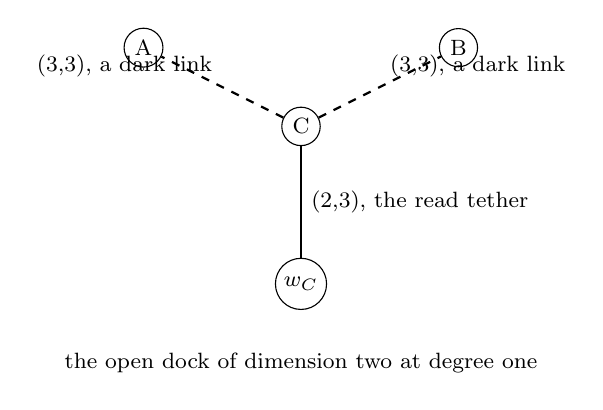
\begin{tikzpicture}[every node/.style={font=\footnotesize}]
\node[circle,draw,inner sep=2pt] (C) at (0,0) {C};
\node[circle,draw,inner sep=2pt] (A) at (-2,1) {A};
\node[circle,draw,inner sep=2pt] (B) at (2,1) {B};
\node[circle,draw,inner sep=2pt] (w) at (0,-2) {$w_C$};
\draw[dashed,thick] (C) -- node[above left] {(3,3), a dark link} (A);
\draw[dashed,thick] (C) -- node[above right] {(3,3), a dark link} (B);
\draw[thick] (C) -- node[right] {(2,3), the read tether} (w);
\node at (0,-3) {the open dock of dimension two at degree one};
\end{tikzpicture}
\caption{The closure site C of the universe web, of dimension three at degree three. Its two (3,3) links to the core sites A and B are the dark links, whose boundary count is the far-end dimension three at every rung, and its (2,3) link to the open dock $w_C$ is the read tether. With the fixed and moving interfaces these are the five elements of the balance.}
\end{figure}
\section{The universality of the move set}\label{mod:X-2-D538680-nmsu-t1}
\begin{chconditional}[The universality of the move set]\label{box:X-2-D538680-nmsu-t1:1}
Conditional on the results this entry rests on, each at its own standing. A move of the theory lies outside the Clifford group: the fourth-root phase generator of the re-matching carries the Weyl letter of the qutrit end to a monomial matrix whose phases are no clock pattern at the cube root of the end and so stands outside the Clifford group of the qutrit end, the same generator and the first transposition stand outside at the ququart end, and every other move stands inside at every end and genre. The groups the unitary one-end moves generate are finite at every end, equal to the Clifford group of the qubit end modulo scalars and parting from it at the qutrit and ququart ends, so the universality of the move set is read with the Clifford group adjoined by name under the Clifford-plus-non-Clifford theorem of the literature, the moves alone generating no dense group at any end.
\end{chconditional}
\chstanding{conditional theorem}
\chdeps{Definitions 1.1 to 1.6, Open result 92.1 and Theorem 92.2 and Open result 231.1}{no theorem beyond it at this release}
Every move is typed against the Clifford group at every end and genre by its action on the Weyl letters, the groups generated by the one-end moves are computed with their orders, and the universality is read with the adjoined group named. The algorithm entries are typed expressible at the first reading and gloss at the second, both readings given and neither adopted. What stands open is the universality of the gate set with the Clifford group adjoined by name and not by a move of the theory. The closure as the computation and the Hadamard as the coherent read stand at their own chapters.
\begin{chbridge}
The Clifford group of a register is the normalizer of its Pauli group, generated by the Hadamard, the phase and the controlled-not gates, and a circuit of Clifford gates alone is simulable classically by the stabilizer formalism. The correspondence is by name.
\end{chbridge}
\begin{chproof}[finite computation]
\textit{The premises.} The axiom and the six definitions of Section~\ref{mod:FRAMEWORK}, definitions. The moves of Section~\ref{mod:I-4-moves-in-one-table}, definitions. The moves as a gate set and the Weyl criterion of Section~\ref{mod:XIII-2-moves-as-a-gate-set-and-the-weyl-criterion}, a theorem. The field equation at the counting face of Section~\ref{mod:X-2-field-equation-at-the-counting-face}, an open result. The step transport, the holonomies, the pairing, the wash, the junction move, the dock move, the Hadamard read and the re-matching, at their own standings. The chain from the axiom to this result is seven chapters deep.

\textit{The procedure.} The input objects are the moves built as exact matrices or channels at the three ends (the qubit, the qutrit and the ququart) and the six genres, forty in all. They are the step transport as the permutation of the link register, the twenty-four holonomies, the pairing as the Bell unitary, the wash as the channel of the cap projectors, the junction move at its holonomy, the dock move at its step, the Hadamard read and the three generators of the re-matching (the first transposition, the full cycle and the fourth-root phase at the first direction). The test applied to each move at each end is the Clifford test. The Weyl letters $X$ (the shift) and $Z$ (the clock at the root of the end), with $ZX=\omega XZ$, are conjugated by the move, and the move is inside the Clifford group when every letter is carried to a Weyl letter at a phase and outside otherwise. The smallest instance is the Hadamard read at the qubit end. It carries $X$ to $Z$ and $Z$ to $X$ at the phase one, inside, and is of order two.

\textit{The totals.} The move is inside at every holonomy (the qubit holonomy carrying $X$ to $z^{12}X$ and $Z$ to itself, the three qutrit holonomies carrying every letter to a Weyl letter at a cube-root or half-turn phase), at the junction holonomy, where it is the identity at 120 of 120 loops, at every dock step, where it is a scalar at 10 of 10 readings, at the Bell unitary and at the re-matching transposition and cycle at the qubit and qutrit ends. It is outside at the fourth-root phase at the qutrit end, which carries $X$ to the monomial matrix
\begin{equation}
\begin{pmatrix}0&0&z^{6}\\ z^{18}&0&0\\ 0&z^{0}&0\end{pmatrix},\qquad z=e^{2\pi i/24},
\end{equation}
a shift of $X$ whose phases are no clock pattern at the cube root of the end, and at the ququart end likewise, with the transposition outside at the ququart end too, 3 of 40 tests outside in all, which is the statement. The groups generated by the unitary one-end moves are finite at every end, of orders $576$ at the qubit end (projective 24, equal to the Clifford group modulo scalars), $10\,368$ at the qutrit end and $6144$ at the ququart end, the latter two parting from the Clifford groups of projective orders $216$ and $768$ at a missing Fourier generator, so the moves alone generate no dense group at any end and the universality is read with the Clifford group adjoined by name.

\textit{The check.} Replacing the fourth-root phase by the identity, reading the step at the fixed near-major register and dropping the Hadamard read each move the inside and outside counts they name. Striking the text moves every cell. The result was reproduced by an independent route, two engines of different construction agreeing at every cell at both runs, with the cycle types of the step transport at 7 of 7, the traces of the holonomies at 24 of 24 and the re-matching orders $32$, $384$ and $6144$ as the controls.
\chcert{120}
\end{chproof}
\section{The universality of the (2,2) increment}\label{mod:X-2-D542409-w-unmi}
\begin{chwall}[The universality of the (2,2) increment]\label{box:X-2-D542409-w-unmi:1}
Face A, the increment per serial (2,2) insertion one cell at every admitted link and step with the (2,2) genre admitted at every web and no second genre admitted at every web, reads no at the universality clause. Face B reads yes with the first parting named: the metric increment per serial (2,2) insertion is one cell 96 at every one of the 1403 links with a qubit end across 77 of the 82 webs of the settled census at every step of the serial run, regardless of the content of the chain, the genre of the entered link, the far dimension, the body or the word, a theorem of the additive metric over the whole census; the serial (2,2) insertion is refused at the five webs with no qubit site, the gluon word of four qutrits, the Higgs word of two ququarts, the Higgs word, the leg piece and the free (3,4) genre of the Higgs-and-carrier entry, so (2,2) is admitted at 77 of 82 webs and no genre of the six is admitted at every web at the reading adopted; the first parting is the gluon word admitting no serial (2,2) insertion; at the readings beside the (3,4) genre attaches at every web under the inserted link alone naming the genre, and every genre at every link under a pair of qubits inserted anywhere, with the increment parting by the ends.
\end{chwall}
\chstanding{open result}
\chdeps{Definitions 1.1 to 1.6, Theorems 9.1 to 9.7 and Open result 9.8, Open result 92.1 and Theorem 92.2 and Theorem 195.1}{no theorem beyond it at this release}
The rule of the metric open result, a qubit site inserted at the entered qubit end with the far link keeping its genre, is applied at every link with a qubit end of the 82 webs of the settled census, and the increment of the register is read at every step; it is one element wherever the insertion is admitted, so the content independence half of the item is a theorem, while the admission itself fails at the five webs that carry no qubit. The field equation at the counting face stands at its own chapter.
\begin{chbridge}
The equivalence principle of the literature states that gravity couples to every form of energy with one and the same constant regardless of its composition, and in a gauge theory the coupling of the carrier is universal across the species it couples to \cite{Einstein1907,Will2014}. The correspondence is by name.
\end{chbridge}
\begin{chproof}[exhaustive census]
\textit{The premises.} The axiom and the six definitions of Section~\ref{mod:FRAMEWORK}, definitions. The link and its six genres of Section~\ref{mod:I-2-link-and-its-six-genres}, definitions. The body-alone office rule of Section~\ref{mod:VIII-2-body-alone-office-rule}, a theorem. The field equation at the counting face of Section~\ref{mod:X-2-field-equation-at-the-counting-face}, an open result. The chain from the axiom to this result is four chapters deep.

\textit{The census.} The set counted is the 82 webs of the settled census, the sixty-four webs of the web table in their order, the proton, the neutron, the deuteron, the one-link web and the two stars of the body-alone entry, the universe web at 444 sites and 551 links, the tau sink at 16 sites and the ten bodies and words of the Higgs-and-carrier entry, 1912 sites and 2381 links with 356 (2,2) links, 255 of the table and 85 of the universe web. The property tested at every link with a qubit end is the increment of the register under the serial insertion, a qubit site inserted at the entered qubit end with the far link keeping its genre, at the steps k 1, 2 and 3; the register is the sum of the caps and the cap of a genre its Born count. The increment reads 96 at every one of 1403 admitted links of 77 webs at every step, the cap of the (2,2) genre,
\begin{equation}
96 = 24 + 18\cdot 2 + 12\cdot 2 + 3\cdot 4,
\end{equation}
the distinct increments one and the first parting none, at a (2,3) link with the far end a qutrit and at a (2,4) link with the far end a ququart alike, since the inserted link is a (2,2) link and the far link keeps its genre; the chains of the metric open result re-meet at 96 at every step, the 1643 uniform chains of the table partition its links by genre, 231, 45, 651, 488, 217 and 11, of which 927 admit the insertion, and the junction stars number 577 with 255 admitting. The webs admitting no link are the five with no qubit site. Over the six genres at the reading adopted the (2,2) genre is admitted at 77 of 82 webs, the (3,3) at 78 with the Higgs word of two ququarts first missing, the (4,4) at 75 with the one-link web first missing, and the three unequal genres at 0 of 82 since the far link cannot keep its genre at an off-diagonal insertion; the second universal genre is none. The smallest case is the electron web at its hub-unit pair, the register 8613 at k 0 and 8709 at k 1, the increment 96, checked by hand from the caps. So face A reads no at the universality clause and face B reads yes with the first parting the gluon word, a parting of the admission clause and of neither form the item words, a typing left to the return. The result is certified at the repository.

\textit{The check.} The electron web struck from the census moves the web count to 81 with the increment unmoved, the inserted sites read as qutrits move the increment to 542, 1036 and 1466 by the far dimension, every web doubled as a disjoint copy doubles the register while the increment stays 96, the genre-to-cap map transposed moves the one cell to 5100, and the text struck excludes the run, 5 of 5 as pinned. The controls read the same at 13 of 13, among them the metric open result re-met at 9 of 9 chains, the caps equal to the Born counts at six genres and the register of the universe web $513\,055$ equal to the sum of the caps over its 551 links. The result was reproduced by an independent route, two engines of different construction agreeing at every cell at both runs.
\chcert{1403}
\end{chproof}
\section{The linear field equation at the counting face}\label{mod:X-2-D543262-w-lnfe}
\begin{chwall}[The linear field equation at the counting face]\label{box:X-2-D543262-w-lnfe:1}
Face A, the washed Laplacian of the (2,2) count equal to the office density at the counting face multiplied by the (2,2) coupling at every settled web, with the non-pair Laplacian the source, reads no at 0 of 21 webs. Face B reads yes with the first parting named: at the 21 rung-reading webs of the ladder of the curvature chapter the washed Laplacian of the (2,2) count and the coupling of the two-point function multiplied by the washed non-pair Laplacian are equal at 0 of 21 webs and at 0 of 1546 cells of the universe web, the first parting at the closure-site body at rung 0 at its first site B31.A, a site of dimension 3 with three links and no (2,2) link, at the diagonal cell reading 0 at the left side against $5/128 + (5/128)\sqrt{2}$ at the right, the coupling $5/384 + (5/384)\sqrt{2}$ multiplied by the source cell 3, and at the universe web at the hub B00.F reading 0 against $5/96 + (5/96)\sqrt{2}$; the two sides part by construction at every cell where a link is not of the pair genre, a rational left cell against a right cell with a nonzero root-two coordinate, and at every cell of a pair link, a nonzero left cell against a zero source cell, so the equation holds at no settled web but one with no links at all; the coupling between the two sides as the trace ratio is an exact rational at every web, 85 over 466 at the universe web and 1 over 4 at the closure-site body, equal to the two-point element at 0 of 21; the source against the office density is equal at 0 of 444 sites of the universe web, B00.F reading 4 against 36.
\end{chwall}
\chstanding{open result}
\chdeps{Definitions 1.1 to 1.6, Theorems 78.1 to 78.3, Theorems 90.1 to 90.4 and Open result 92.1 and Theorem 92.2}{no theorem beyond it at this release}
The washed Laplacian of the (2,2) count is built and washed at every web of the ladder, the source is built as the washed Laplacian of the links not of the pair genre and compared with the office density at every site, the coupling is printed at every web as the trace ratio and against the two-point element, and the two sides of the linear equation are compared cell by cell. The two sides live on disjoint links and in different rings, so the equation names an open result at its first site. The curvature and the field equation stand at their own chapters.
\begin{chbridge}
The linearized field equation of gravitation in the literature sets the Laplacian of the metric perturbation proportional to the energy density of its source with the gravitational constant as the coupling, and in electrodynamics the Laplacian of the potential is proportional to the charge density with the fine-structure constant setting the strength \cite{Einstein1916,Peskin1995}. The correspondence is by name.
\end{chbridge}
\begin{chproof}[exhaustive census with its exact part]
\textit{The premises.} The axiom and the six definitions of Section~\ref{mod:FRAMEWORK}, definitions. The curvature as the graph Laplacian washed over the ladder of Section~\ref{mod:X-1-curvature-as-the-graph-laplacian-washed-over-the-ladder}, a theorem. The field equation at the counting face of Section~\ref{mod:X-2-field-equation-at-the-counting-face}, an open result. The Ward identity and the anomaly sums of Section~\ref{mod:IV-8-ward-identity-and-the-anomaly-sums}, a theorem. The chain from the axiom to this result is five chapters deep.

\textit{The census.} The set counted is the 21 rung-reading webs of the ladder of the curvature chapter at the three readings and rungs 0 to 6, rebuilt from the closure entries at 21 of 21 webs and 105 of 105 ladder cells. At every web the left side is the washed Laplacian of the (2,2) count, symmetric with the row sums zero at 21 of 21, the trace 170 at the universe web and 6 at the closure-site body; the source is the washed Laplacian of the links not of the pair genre, the trace 932 at the universe web and 24 at the closure-site body, the sum of the two sides equal to the washed Laplacian at every cell of 21 of 21 webs; the office density at the reading adopted is the first-power flux at a site, 8836 over the universe web; the coupling is read by key at the dressing table of the two-point entry, $(30 + 30\sqrt{2})/2304 = 5/384 + (5/384)\sqrt{2}$. The property tested at every cell is the equality of the left cell with the coupling multiplied by the source cell: at the universe web 0 of 1546 cells and at the closure-site body 0 of 42, the first parting at the first web of the frozen order, the closure-site body at rung 0 at its first site B31.A, the left cell 0 against $(5/384 + (5/384)\sqrt{2})\cdot 3 = 5/128 + (5/128)\sqrt{2}$, the smallest case worked at the figure. The coupling between the two sides as the trace ratio reads 85 over 466 at the universe web and 1 over 4 at the closure-site body, an exact rational at 21 of 21 webs and equal to the two-point element at 0 of 21; the source against the office density is equal at 0 of 444 sites. So the rule pinned ahead reads face A no and face B yes. The result is certified at the repository.

\textit{The check.} The source struck, the (2,3) Laplacian in place of the (2,2), the coupling struck to one, the text struck and the pair ket at the join appended as a twenty-second web each move the cells they name, 5 of 5 as pinned. The controls read the same at 14 of 15 at the pinned engines and at 15 of 15 at the return route, the one spelling of the serial increment keys re-keyed as sparse maps. The result was reproduced by an independent route, two engines of different construction agreeing at every cell at both runs.
\chcert{1546}
\end{chproof}
\begin{figure}[h]
\centering
\begin{adjustbox}{max width=\linewidth}\begin{tabular}{lll}
\hline
site & the left cell & the coupling multiplied by the source cell \\
\hline
B31.A & 0 & $(5/384 + (5/384)\sqrt{2})\cdot 3 = 5/128 + (5/128)\sqrt{2}$ \\
\hline
\end{tabular}\end{adjustbox}
\caption{The smallest case, the closure-site body at rung 0 at its first site B31.A: the left cell 0 against the coupling multiplied by the source cell 3, a rational against an element with a nonzero root-two coordinate.}
\end{figure}
\section{The nonlinear field equation at the counting face}\label{mod:X-2-D543652-w-nlfe}
\begin{chwall}[The nonlinear field equation at the counting face]\label{box:X-2-D543652-w-nlfe:1}
Face A, the nonlinear field equation closing at every settled web, the (2,2) count plus the vacuum term equal to the coupling of the two-point function multiplied by the office density plus the count itself, closing under the row-sum-zero operator with the density conserved along the chains and the vacuum term uniform, reads no at 0 of 21 webs. Face B reads yes with the first parting named: at the 21 rung-reading webs of the ladder of the curvature chapter the equation closes at 0 of 444 sites of the universe web and at no site of any web, the first parting at the closure-site body at rung 0 at its first site B31.A under the readings closure and sources, the count 0 plus the vacuum term at the depth 3 of the site, $1/23\,328$, against the coupling multiplied by the density 30, $25/64 + (25/64)\sqrt{2}$, and the self-source 0 against the office density 30, at the universe web at B00.F $1/839\,808$ against $15/32 + (15/32)\sqrt{2}$; the two sources part by construction at every site with a link; the closure under the row-sum-zero operator reduces to the conservation of the density along the chains at every settled web, the operator applied to the count zero everywhere with every chain one link, and holds at 430 of 444 sites and 78 of 85 chains of the universe web and at every site and chain of the fourteen webs of the first two readings, the first unconserved chain from B07.w1 to B07.b3 at 4 against 12; the vacuum term at the depth of the site is uniform at 0 of 21 webs, 14 distinct values at the universe web, with the term $1/1\,088\,391\,168$ at the depth exponent 6 re-met by key.
\end{chwall}
\chstanding{open result}
\chdeps{Definitions 1.1 to 1.6, Theorems 90.1 to 90.4, Open result 92.1 and Theorem 92.2 and Theorem 115.1}{no theorem beyond it at this release}
The two sources of the nonlinear equation, the count at a site and the office density, are built and compared at every site of every web of the ladder, the closure under the row-sum-zero operator and the conservation of the density along the chains are read at every site and chain, and the vacuum term is printed at every site at the depth read there. The count is not its own source beside the density at the coupling of the two-point function at any web, and the closure under the operator is the conservation of the density. The curvature and the field equation stand at their own chapters.
\begin{chbridge}
The field equations of gravitation are nonlinear, the geometry sourcing itself, their divergence vanishes by the Bianchi identity so that the source is conserved, and the cosmological constant enters as one term uniform over space \cite{Einstein1916,Einstein1917,Wald1984}. The correspondence is by name.
\end{chbridge}
\begin{chproof}[finite computation with its census and its exact part]
\textit{The premises.} The axiom and the six definitions of Section~\ref{mod:FRAMEWORK}, definitions. The curvature as the washed Laplacian of Section~\ref{mod:X-1-curvature-as-the-graph-laplacian-washed-over-the-ladder}, a theorem. The field equation at the counting face of Section~\ref{mod:X-2-field-equation-at-the-counting-face}, an open result. The cosmological term at the depth exponent of Section~\ref{mod:X-6-cosmological-term-at-the-depth-exponent}, a theorem. The chain from the axiom to this result is five chapters deep.

\textit{The procedure.} At every one of the 21 webs of the ladder the row-sum-zero operator is the washed Laplacian of the (2,2) links with the count on its diagonal, symmetric with the row and column sums zero, the count sum 170 at the universe web and 1 at each of the six qubit legs of the closure-site body; the self-source is the count at the site; the office density is the first-power flux at the site, the sum over its links of the product of the end dimensions; the vacuum term at a site is the closure constant 2 over the whole register 36 to the depth read at the site, the depth its eccentricity by breadth-first passage count over the links of its component. The equation of the item at a site reads the count plus the vacuum term against the coupling of the two-point function multiplied by the density plus the count; the closure reading applies the operator to both sides, under which the vacuum term drops by the row sums zero; the conservation reading asks the density to be one value along every chain, the chains the components of the pair links.

\textit{The totals.} The two sources are equal at 0 of 444 sites of the universe web, the first parting B00.F at the count 0 against the density 36, and at 0 of 12 sites of the closure-site body, B31.A at 0 against 30, since a link adds one to the count of each end and the product of the end dimensions, at least four, to the density of each end. From the coupling and the density at B31.A, by the product, we obtain the right side
\begin{equation}
\Bigl(\frac{5}{384} + \frac{5}{384}\sqrt{2}\Bigr)\cdot 30 + 0 = \frac{25}{64} + \frac{25}{64}\sqrt{2}
\end{equation}
against the left side $0 + 2/36^{3} = 1/23\,328$ at the depth 3, the smallest case worked on the page, and at B00.F the left side $2/36^{4} = 1/839\,808$ against $15/32 + (15/32)\sqrt{2}$; a rational stands against an element with a nonzero root-two coordinate at every site unless the density and the count are both zero, so the equation closes at 0 of 21 webs. The operator applied to the count is zero at every site of every web, every chain being one link with the count 1 at both ends, so the closure under the operator reads the operator applied to the density alone, equal at 430 of 444 sites of the universe web with the first parting B07.b3 at 0 against $5/48 + (5/48)\sqrt{2}$, at 12 of 12 sites of the closure-site body at every rung of the first two readings and at every site of 14 of 21 webs; the density is one value along 78 of 85 chains of the universe web, the first unconserved from B07.w1 to B07.b3 at 4 against 12, along the three chains of the closure-site body at 12 and 12, and along every chain of 14 of 21 webs, the closure-parting sites equal to the unconserved sites at 21 of 21 webs. The depth census of the universe web reads 1, 8, 18, 48, 72, 92, 80, 38, 44, 10, 18, 4, 7, 4 at the depths 1 to 14 with 14 distinct term values, the first parting B00.G at the depth 3 against B00.F at the depth 4, and at the closure-site body three distinct values with the first parting at the hub B31.H1 at the depth 4 against 3, uniform at 0 of 21 webs; the term at the depth exponent 6, $1/1\,088\,391\,168$, is one value at every site by construction and equals the term of the curvature-coefficient open result and the counting-face open result by key. The first order beside, the diagonal reading of the linear equation, parts at B31.A and B00.F at the cells of that open result, re-met by key at 25 of 25. So the rule pinned ahead reads face A no and face B yes with the first parting named.

\textit{The check.} The self-source struck moves the self-source sum from 170 to 0, the (2,3) count in place of the (2,2) moves the count sum to 68, the vacuum term struck moves the left cell to 0 with the vacuum reading uniform by the strike, the text struck excludes the run, and the pair ket appended as a twenty-second web moves the compared webs to 22 of 22, 5 of 5 as pinned. The controls read the same at 17 of 17, among them the linear equation re-met at its coupling at 25 of 25 keys and the curvature-coefficient open result at 30 of 30 cells. The result was reproduced by an independent route, two engines of different construction agreeing at every cell at both runs.
\chcert{444}
\end{chproof}
\begin{figure}[h]
\centering
\begin{adjustbox}{max width=\linewidth}\begin{tabular}{lll}
\hline
site & the left side & the right side \\
\hline
B31.A at the depth 3 & $2/36^{3} = 1/23\,328$ & $25/64 + (25/64)\sqrt{2}$ \\
B00.F at the depth 4 & $2/36^{4} = 1/839\,808$ & $15/32 + (15/32)\sqrt{2}$ \\
\hline
\end{tabular}\end{adjustbox}
\caption{The smallest case, the site B31.A at the depth 3, with the hub B00.F beside: a rational on the left against an element with a nonzero root-two coordinate on the right, so the equation closes at 0 of 21 webs.}
\end{figure}
\section{The field equation as the first law}\label{mod:X-2-D543764-w-flfw}
\begin{chwall}[The field equation as the first law]\label{box:X-2-D543764-w-flfw:1}
Face A, the count of records crossing the horizon at one depth step one proportion of the office flux across it at every step with the coupling of the two-point function its constant, reads no. Face B reads yes with the first parting named: at the horizon web the records newly hidden at the six depth steps read 0, 3, 0, 3, 0, 3 at the open-end face and 0, 3, 3, 3, 3, 3 at the docking order, while the first-power flux through the fixed cut is 24 at every rung, the two (3,3) wires at 9 each and the (2,3) tether at 6, and through the moving cut 24 then 12 at every rung of the open-end face and 24, 12, 30, 14, 14, 18, 24 at the docking order, so the ratio of the crossing count to the flux reads 0 at the first step of every series and 1 over 8 at the second step at the fixed cut, parting at step 2 at 4 of 4 series; against the coupling $5/384 + (5/384)\sqrt{2}$ the ratio, a rational at every step, parts at 24 of 24 steps, the first parting at the open-end face at the fixed interface at step 1, 0 against the coupling; against the area-law coefficient at the count reading, 1 over 4, 1 over 4, 1 over 2, 1 over 2, 3 over 4, 3 over 4 and 1 across the rungs of the fixed cut, the ratio parts at 24 of 24 steps; the counting-face equation of the linear open result re-derived at the ratio holds at 0 of 18 settled webs with a step.
\end{chwall}
\chstanding{open result}
\chdeps{Definitions 1.1 to 1.6, Open result 92.1 and Theorem 92.2 and Theorems 99.1 and 99.2, Open results 99.3 and 99.4, Theorem 99.5 and Open result 99.6}{no theorem beyond it at this release}
The records newly hidden at each depth step of the horizon web are counted from the hidden records of the area-law open result, the first-power flux through the crossing links is summed at every cut and rung, and their ratio is compared with the coupling of the two-point function and with the area-law coefficient at every step, the linear equation then re-derived with that ratio in place of the coupling. No record crosses at the first step while the flux is 24, so the ratio is zero where the coupling is not, and three records cross at the second step, so it is no constant of the web. The field equation, the horizon and the area law stand at their own chapters.
\begin{chbridge}
The first law of horizon thermodynamics in the literature relates the entropy change of a horizon to the energy flux across it in one proportion whose constant is the temperature, and the field equation itself follows from that law applied at every point \cite{Bekenstein1973,Jacobson1995}. The correspondence is by name.
\end{chbridge}
\begin{chproof}[exhaustive census]
\textit{The premises.} The axiom and the six definitions of Section~\ref{mod:FRAMEWORK}, definitions. The field equation at the counting face of Section~\ref{mod:X-2-field-equation-at-the-counting-face}, an open result. The horizon at every rung of Section~\ref{mod:X-3-horizon-at-every-rung-and-the-horizon-web-as-a-seeded-saturation}, a theorem. The area law at the cut of the chapter titled The area law at the cut (chapter~\ref{mod:X-2a-D542325-w-arlw}), an open result. The chain from the axiom to this result is five chapters deep.

\textit{The census.} The set counted is the depth steps of the horizon web at the two admitted readings of the attachment site, the open-end face and the docking order, at the fixed and the moving cut, 24 step cells of the four series, with the closure-site face beside at rung 0 alone. The hidden records are read from the area-law open result by locator, 3, 3, 6, 6, 9, 9, 12 at the open-end face and 3, 3, 6, 9, 12, 15, 18 at the docking order, equal to the closure table of the horizon chapter; the records newly hidden at a step are the hidden count at the rung less the count at the rung beneath, 0, 3, 0, 3, 0, 3 and 0, 3, 3, 3, 3, 3 across the steps 1 to 6, exact at 36 of 36 step cells over the readings. The crossing links of the area-law open result are parsed into their end dimensions and the act of a link read as the product of its end dimensions, the first-power rule of the counting-face chapter, so the flux through the fixed cut is
\begin{equation}
9 + 9 + 6 = 24
\end{equation}
at every rung, the two (3,3) wires and the (2,3) tether, and through the moving cut 24, 12, 12, 12, 12, 12, 12 at the open-end face and 24, 12, 30, 14, 14, 18, 24 at the docking order, every flux a nonzero integer at 42 of 42 cuts, equal to the flux cells of the counting-face chapter at every element and rung. The ratio of the crossing count to the flux at the lower rung of the pair reads 0, 1 over 8, 0, 1 over 8, 0, 1 over 8 at the open-end face at the fixed cut, 0, 1 over 4, 0, 1 over 4, 0, 1 over 4 at its moving cut, 0 then 1 over 8 at every step at the docking order at the fixed cut and 0, 1 over 4, 1 over 10, 3 over 14, 3 over 14, 1 over 6 at its moving cut, parting at step 2 at 4 of 4 series, the smallest case the first two steps at the fixed cut, 0 over 24 then 3 over 24. Against the coupling $5/384 + (5/384)\sqrt{2}$ the ratio differs at 24 of 24 steps, the difference at the first step minus the coupling and at the second step $43/384 - (5/384)\sqrt{2}$; against the area-law coefficient at the count reading, 1 over 4, 1 over 4, 1 over 2, 1 over 2, 3 over 4, 3 over 4, 1 at the fixed cut, it differs at 24 of 24; the linear equation re-derived with the ratio at the fixed cut in place of the coupling holds at 0 of 18 webs with a step, the first parting at the closure-site body at rung 1 at its first pair site B31.q1 reading 1 against 0, and the linear open result itself is re-met at its own coupling at every web with its first parting cell string for string. So the rule pinned ahead reads face A no and face B yes with the first parting the coupling at the open-end face at the fixed interface at step 1, the proportionality itself parting one step on.

\textit{The check.} The hidden records at rung 2 struck move the step count to minus 3, the (2,3) flux in place of the office flux moves the flux to 6 with every ratio, the coupling struck to one moves every difference, a horizon with no hidden record moves the series letter to constant at every step, and the text struck excludes the run, 5 of 5 as pinned. The controls read the same at 13 of 13. The result was reproduced by an independent route, two engines of different construction agreeing at every cell at both runs.
\chcert{24}
\end{chproof}
\par\medskip\noindent{\itshape The next chapter reads the horizon at every rung.}\label{narr:close:10-2}\par
\section{The area law at the horizon web}\label{mod:X-2a-D542325-w-arlw}
\chdesig{6-2a}{10-2a}{X-2a-D542325-w-arlw}{X-2a-D542325-w-arlw}
\begin{chwall}[The area law at the horizon web]\label{box:X-2a-D542325-w-arlw:1}
Face A, the hidden records proportional to the counted (2,2) crossings at every rung with the constant printed as an exact element, reads no. Face B reads yes with the first parting named: at the horizon web, the universe web of the hand-off at 444 sites and 551 links with its rungs 0 to 6 as the closure table of the horizon chapter specifies them at the open-end face and the docking-order face, the cut at the slot B31.C severs two (3,3) wires and the (2,3) tether at every rung and the cut at the newest rung severs (2,3), (2,4) and (3,4) links alone, the counted (2,2) crossings 0 at 7 of 7 rungs at every reading and interface, so the area at the (2,2) face reads 0 at every rung while the hidden records read 3, 3, 6, 6, 9, 9, 12 at the open-end face and 3, 3, 6, 9, 12, 15, 18 at the docking order, the ratio of the hidden records to the counted crossings undefined at every rung of the four series, the first parting at the open-end face at the fixed interface at rung 0, the hidden records 3 against the counted crossings 0; the series beside part too, the hidden records over every crossing link 1, 1, 2, 2, 3, 3, 4 at the fixed interface of the open-end face parting at rung 2, and over the summed caps 2391 at the fixed interface parting alike.
\end{chwall}
\chstanding{open result}
\chdeps{Definitions 1.1 to 1.6, Theorems 99.1 and 99.2, Open results 99.3 and 99.4, Theorem 99.5 and Open result 99.6 and Theorems 113.1 and 113.2}{no theorem beyond it at this release}
The cut of the horizon web is censused by genre at every rung at two admitted readings of the attachment site and at the fixed and the moving interface, the area read as the counted (2,2) crossings at the increment of the metric open result with the summed caps, the ticks and the tower beside, and the hidden records counted as the records of the closure at the qubit ends. The (2,2) links sit inside the bodies and never at the cut, so no constant of proportion exists at any rung and the area law at the (2,2) face is an open result at rung 0. The horizon at every rung and the register tower stand at their own chapters.
\begin{chbridge}
The entropy of a black hole in the literature is proportional to the area of its horizon, one quarter of the area in Planck units, and the holographic principle bounds the degrees of freedom of a region by the area of its boundary \cite{Bekenstein1973,Hawking1975,Bousso2002}. The correspondence is by name.
\end{chbridge}
\begin{chproof}[finite computation with its census and its exact part]
\textit{The premises.} The axiom and the six definitions of Section~\ref{mod:FRAMEWORK}, definitions. The horizon at every rung of Section~\ref{mod:X-3-horizon-at-every-rung-and-the-horizon-web-as-a-seeded-saturation}, a theorem. The area law at the cut of the chapter titled The area law at the cut (chapter~\ref{mod:X-2a-D542325-w-arlw}), at its standing. The register tower of Section~\ref{mod:X-5-register-tower-and-the-metric}, a theorem. The chain from the axiom to this result is five chapters deep.

\textit{The procedure.} The universe web of the hand-off is parsed whole at 444 sites, 551 links, 27 components and the genres 85, 34, 229, 134, 67 and 2 at (2,2) to (4,4) with 54 sites of degree one, the open dock B31.wC of dimension 2, the tether C to wC a (2,3) link, the slot B31.C of dimension 3 at degree 3 and the star severed by the cut, A to C and B to C at (3,3) and C to wC at (2,3). The rungs 0 to 6 are read at the open-end face, the chain of alternating dimensions joined by (2,3) links, and at the docking order, the six leaves docked at the named sites, the closure-site face refused beyond rung 0 as the closure table prints it. At the fixed interface, the cut at the slot, and at the moving interface, the cut at the attachment site of the newest rung, the crossing links are censused by genre and the (2,2) crossings counted; the area is the counted crossings multiplied by the increment 96 of the metric open result, the summed area every crossing link at its cap, and the hidden records are counted as 3 per qubit end behind the cut and 0 per qutrit end under the sign clause.

\textit{The totals.} At the fixed interface the census reads 0, 1, 0, 2, 0, 0 at the six genres at every rung and reading, the counted (2,2) crossings 0, the total 3 and the horizon counts 9 at both alphabets; at the moving interface the open-end face severs the two (2,3) links from rung 1 and the docking order severs (2,3), (2,4) and (3,4) links alone, the totals 3, 2, 3, 2, 2, 2, 3, so the counted (2,2) crossings read 0 at 28 of 28 cells. The counted area is 0 at every rung, the summed area at the fixed interface
\begin{equation}
1036 + 1036 + 319 = 2391
\end{equation}
at every rung, 638 at the moving interface of the open-end face from rung 1 and 2391, 638, 4425, 1225, 1225, 2372, 2691 at the docking order, with the ticks 3 at the fixed interface and the tower of the depth-scale chapter beside, 24 multiplied by 36 to the rung, equal at 7 of 7 rungs to the horizon chapter, the cap-wave census and the depth-scale tower. The qubit ends behind the cut read 1, 1, 2, 2, 3, 3, 4 at the open-end face and 1, 1, 2, 3, 4, 5, 6 at the docking order, so the hidden records read 3, 3, 6, 6, 9, 9, 12 and 3, 3, 6, 9, 12, 15, 18, equal to the closure table at 15 of 15 cells; the smallest instance is rung 0, one qubit end behind the fixed cut and 3 hidden records against 0 counted crossings. The ratio of the hidden records to the counted crossings is undefined at every one of the 28 cells of the four series, so face A reads no and face B reads yes at the open-end face at the fixed interface at rung 0; beside, the ratio over every crossing link reads 1, 1, 2, 2, 3, 3, 4 at the fixed interface and parts at rung 2, and the ratio over the summed caps reads 1 over 797 at rung 0 and parts at rung 2 at the fixed interface and at rung 1 at the moving interfaces, every ratio an exact rational or undefined. The result is certified at the repository.

\textit{The check.} The rung 3 struck moves the hidden records at the docking order from 9 to 6, the (2,3) crossings in place of the (2,2) moves the counted crossings to 1 with the ratios then defined and parting, the horizon shifted to B31.A moves the census to two (3,3) wires and a (3,4) link, the unwashed count at the Weyl letters moves the hidden records from 3 to 11, and the text struck excludes the run, 5 of 5 as pinned. The controls read the same at 12 of 12, among them the closure table at 21 of 21, the horizon table at 12 of 12 and the cap-wave census at 10 of 10. The result was reproduced by an independent route, two engines of different construction agreeing at every cell at both runs.
\chcert{300}
\end{chproof}
\begin{figure}[htbp]\centering
\setlength{\unitlength}{1mm}
\begin{picture}(160,36)(0,0)
\put(2,26){\framebox(8,6){\scriptsize 3}}
\put(2,4){\framebox(8,6){\scriptsize 3}}
\put(24,15){\framebox(8,6){\scriptsize 3}}
\put(20,11){\makebox(16,3){\tiny B31.C}}
\put(50,15){\framebox(8,6){\scriptsize 2}}
\put(46,11){\makebox(16,3){\tiny B31.wC}}
\qbezier(10,29)(17,25)(24,21)
\qbezier(10,7)(17,11)(24,15)
\qbezier(32,18)(41,18)(50,18)
\put(20,8){\dashbox{1}(17,20){}}
\put(14,30){\makebox(28,3){\tiny the fixed cut}}
\put(8,26){\makebox(16,3){\tiny (3,3) cap 1036}}
\put(8,8){\makebox(16,3){\tiny (3,3) cap 1036}}
\put(33,19){\makebox(16,3){\tiny (2,3) cap 319}}
\put(62,28){\makebox(98,3){\scriptsize the links crossing the cut: A-C:(3,3); B-C:(3,3); C-wC:(2,3); the wholes 81, 81 and 36, the cut register 236196}}
\put(62,22){\makebox(98,3){\scriptsize the increment 96 per serial (2,2) link; the caps by genre 22:96, 23:319, 24:906, 33:1036, 34:2053, 44:5100}}
\put(62,16){\makebox(98,3){\scriptsize the formal log of the cut register $2\log 2+10\log 3$; the dark register 6561 (the two (3,3) wires)}}
\put(62,10){\makebox(98,3){\scriptsize the universe web of record at 444 sites and 551 links; the counted (2,2) crossings 0 at every rung}}
\end{picture}
\par\smallskip
{\scriptsize\setlength{\tabcolsep}{3pt}\begin{adjustbox}{max width=\linewidth}\begin{tabular}{lrrrrrrr}
rung & 0 & 1 & 2 & 3 & 4 & 5 & 6 \\
\hline
\multicolumn{8}{l}{\textit{the fixed cut at both faces}} \\
links crossing the cut by genre & (2,3): 1, (3,3): 2 & (2,3): 1, (3,3): 2 & (2,3): 1, (3,3): 2 & (2,3): 1, (3,3): 2 & (2,3): 1, (3,3): 2 & (2,3): 1, (3,3): 2 & (2,3): 1, (3,3): 2 \\
counted (2,2) crossings & 0 & 0 & 0 & 0 & 0 & 0 & 0 \\
counted area & 0 & 0 & 0 & 0 & 0 & 0 & 0 \\
summed area over the caps & 2391 & 2391 & 2391 & 2391 & 2391 & 2391 & 2391 \\
ticks, one per crossing link & 3 & 3 & 3 & 3 & 3 & 3 & 3 \\
cut register & 236196 & 236196 & 236196 & 236196 & 236196 & 236196 & 236196 \\
(2,2) depth of the cut & 0 & 96 & 192 & 288 & 384 & 480 & 576 \\
\hline
\multicolumn{8}{l}{\textit{the open-end face}} \\
hidden records & 3 & 3 & 6 & 6 & 9 & 9 & 12 \\
records over the counted (2,2) crossings & undefined & undefined & undefined & undefined & undefined & undefined & undefined \\
records over every crossing link & 1 & 1 & 2 & 2 & 3 & 3 & 4 \\
records over the summed area & $1/797$ & $1/797$ & $2/797$ & $2/797$ & $3/797$ & $3/797$ & $4/797$ \\
records over the log of the cut register & $3/(2\log 2+10\log 3)$ & $3/(2\log 2+10\log 3)$ & $3/(1\log 2+5\log 3)$ & $3/(1\log 2+5\log 3)$ & $9/(2\log 2+10\log 3)$ & $9/(2\log 2+10\log 3)$ & $6/(1\log 2+5\log 3)$ \\
records over the (2,2) depth of the cut & undefined & $1/32$ & $1/32$ & $1/48$ & $3/128$ & $3/160$ & $1/48$ \\
register at the moving cut & 236196 & 1296 & 1296 & 1296 & 1296 & 1296 & 1296 \\
\hline
\multicolumn{8}{l}{\textit{the docking-lemma face}} \\
hidden records & 3 & 3 & 6 & 9 & 12 & 15 & 18 \\
records over the counted (2,2) crossings & undefined & undefined & undefined & undefined & undefined & undefined & undefined \\
records over every crossing link & 1 & 1 & 2 & 3 & 4 & 5 & 6 \\
records over the summed area & $1/797$ & $1/797$ & $2/797$ & $3/797$ & $4/797$ & $5/797$ & $6/797$ \\
records over the log of the cut register & $3/(2\log 2+10\log 3)$ & $3/(2\log 2+10\log 3)$ & $3/(1\log 2+5\log 3)$ & $9/(2\log 2+10\log 3)$ & $6/(1\log 2+5\log 3)$ & $15/(2\log 2+10\log 3)$ & $9/(1\log 2+5\log 3)$ \\
records over the (2,2) depth of the cut & undefined & $1/32$ & $1/32$ & $1/32$ & $1/32$ & $1/32$ & $1/32$ \\
register at the moving cut & 236196 & 1296 & 746496 & 2304 & 2304 & 5184 & 186624 \\
\hline
\end{tabular}\end{adjustbox}}
\caption{The area law per rung at the fixed cut of the horizon web of record: the links crossing the cut by genre, the counted (2,2) crossings, the counted and summed areas in the units of the increment and the caps, the hidden records at the two faces, the cut register with its formal log and the coefficient of the hidden records to the log at every rung 0 to 6 (the area law). No (2,2) link crosses the cut at any rung, so the ratio of the hidden records to the counted crossings is undefined at every rung, and the cut register is one register at every rung while the hidden records grow by three per qubit rung.}\label{fig:X-2a-542325-arealaw}
\end{figure}
\begin{figure}[h]
\centering
\begin{adjustbox}{max width=\linewidth}\begin{tabular}{lrrr}
\hline
rung at the open-end face & qubit ends behind the cut & hidden records & counted crossings \\
\hline
0 & 1 & 3 & 0 \\
6 & 4 & 12 & 0 \\
\hline
\end{tabular}\end{adjustbox}
\caption{The smallest instance at the fixed interface, rung 0: one qubit end behind the cut and 3 hidden records against 0 counted crossings, the ratio undefined, as at every one of the 28 cells; rung 6 beside.}
\end{figure}
\section*{The Horizon}
\addcontentsline{toc}{section}{The Horizon}
\section{The horizon at every rung and the horizon web as a seeded saturation}\label{mod:X-3-horizon-at-every-rung-and-the-horizon-web-as-a-seeded-saturation}
\chdesig{6-3}{10-3}{X-3-horizon-at-every-rung-and-the-horizon-web-as-a-seeded-saturation}{X-3-D543792-abrh-t1}
\label{narr:open:10-3}Theorem~99.1 reads the horizon at every rung as a seeded saturation, Theorem~99.2 the horizon register face at the closure, Theorem~99.5 the horizon web as a non-sink at the bound, and the open results beside them, Open result~99.3, Open result~99.4, Open result~99.6, Open result~100.1 and Open result~101.1, carry the horizon web to the cap.
\begin{chconditional}[The horizon at every rung as a seeded saturation]\label{box:X-3-horizon-at-every-rung-and-the-horizon-web-as-a-seeded-saturation:1}
Conditional on the results this entry rests on, each at its own standing. The iterated closure of the universe web under the rule of records, built at rungs zero to six at the three readings of the attachment site, carries the horizon count at the closure interface at every rung, the fixed interface at nine, the register fraction of every readout unchanged, and the point group of the one-rung web the dihedral group of order eight.
\end{chconditional}
\chstanding{conditional theorem}
\chdeps{Definitions 1.1 to 1.6, Open results 241.1 and 241.2, Theorems 241.3 and 241.4 and Open results 241.5 to 241.7 and Open results 245.1 and 245.2, Theorem 245.3, Open results 245.4 to 245.8 and Theorem 245.9}{the theorems of Chapters 6-2, 6-2a, 6-3 to 6-4, 6-6}
\begin{chconditional}[Horizon register face at the closure]\label{box:X-3-horizon-at-every-rung-and-the-horizon-web-as-a-seeded-saturation:2}
Conditional on depth scale at the register tower, horizon at every rung from iterated closure and boundary count at the counting face, each at its own standing. The gravitational coupling object and the expansion object meet at one face of the horizon register, the valence face at the rung count sixty-three, both read through the same closure interface with the register exponent equal to the closure count there, where the closure is saturated at its free-direction bound, while at the cap face the closure count parts from its bound.
\end{chconditional}
\chstanding{conditional theorem}
\chdeps{Definitions 1.1 to 1.6, Open results 241.1 and 241.2, Theorems 241.3 and 241.4 and Open results 241.5 to 241.7 and Open results 245.1 and 245.2, Theorem 245.3, Open results 245.4 to 245.8 and Theorem 245.9}{the theorems of Chapters 6-2, 6-2a, 6-3 to 6-4, 6-6}
\begin{chwall}[The first rungs as the iterated closure]\label{box:X-3-horizon-at-every-rung-and-the-horizon-web-as-a-seeded-saturation:3}
The first rungs from the first closure are an exact object at every reading, but the closure admits more than one reading at the first rung, the three readings of the attachment site parting there.
\end{chwall}
\chstanding{open result}
\chdeps{Definitions 1.1 to 1.6, Open results 241.1 and 241.2, Theorems 241.3 and 241.4 and Open results 241.5 to 241.7 and Open results 245.1 and 245.2, Theorem 245.3, Open results 245.4 to 245.8 and Theorem 245.9}{the theorems of Chapters 6-2, 6-2a, 6-3 to 6-4, 6-6}
\begin{chwall}[The horizon web as a seeded saturation, second entry]\label{box:X-3-horizon-at-every-rung-and-the-horizon-web-as-a-seeded-saturation:4}
The universe web, saturated from itself under the moves at the seed-site-count bound, is no seeded sink within the budget tried and stops at no wave reached, the depth a lower bound of three, and the same at a budget raised fourfold under the removing and pairing moves alone.
\end{chwall}
\chstanding{open result}
\chdeps{Definitions 1.1 to 1.6, Open results 241.1 and 241.2, Theorems 241.3 and 241.4 and Open results 241.5 to 241.7 and Open results 245.1 and 245.2, Theorem 245.3, Open results 245.4 to 245.8 and Theorem 245.9}{the theorems of Chapters 6-2, 6-2a, 6-3 to 6-4, 6-6}
\begin{chconditional}[The horizon web as a non-sink at the bound]\label{box:X-3-horizon-at-every-rung-and-the-horizon-web-as-a-seeded-saturation:5}
Conditional on the results this entry rests on, each at its own standing. The imbalance readout of the universe web at the site bound is an output at every kind of move: the forward edges at the first wave are complete, every readout an integer and every rate cell an exact positive rational at every kind with an edge, and the expansion structure and the dark-fraction structure are exact rational cells, under the site bound and the cut wave of the depth result.
\end{chconditional}
\chstanding{conditional theorem}
\chdeps{Definitions 1.1 to 1.6, Open results 241.1 and 241.2, Theorems 241.3 and 241.4 and Open results 241.5 to 241.7 and Open results 245.1 and 245.2, Theorem 245.3, Open results 245.4 to 245.8 and Theorem 245.9}{the theorems of Chapters 6-2, 6-2a, 6-3 to 6-4, 6-6}
\begin{chwall}[The field equation at the horizon web]\label{box:X-3-horizon-at-every-rung-and-the-horizon-web-as-a-seeded-saturation:6}
The field equation of the counting face, evaluated at the universe web as a non-sink, closes at no depth and parts at the same side as the sink reading, first at the hub kind at the depth three.
\end{chwall}
\chstanding{open result}
\chdeps{Definitions 1.1 to 1.6, Open results 241.1 and 241.2, Theorems 241.3 and 241.4 and Open results 241.5 to 241.7 and Open results 245.1 and 245.2, Theorem 245.3, Open results 245.4 to 245.8 and Theorem 245.9}{the theorems of Chapters 6-2, 6-2a, 6-3 to 6-4, 6-6}
The universe web is closed under the rule of records at the three readings of the attachment site, the counts at the closure interface read at every rung, the register fraction carried through the rungs and the point group adopted. The coupling and expansion objects are re-derived from the hand-off at the valence and cap faces, both read through the fixed interface, and the closure count compared with the free-direction bound at each. The forward edges at the first wave are re-built from the depth result and sorted at the token map, the imbalance readout and the rate cell computed at every kind of move. The four open questions each evaluate their object and record its parting. The reading of the attachment site at which the horizon register is read is fixed by no result, the horizon web as a non-sink holds under the bound, and the termination wave of the universe web stands at no wave reached.
\begin{chbridge}
One term of this chapter stands beyond the framework, defined at its first use, \rosetta{the register tower}{a tower of Hilbert spaces of growing dimension}. The correspondence is by name.
\end{chbridge}
\begin{chproof}[finite computation with its census and its exact part]
\textit{The premises.} The axiom and the six definitions of Section~\ref{mod:FRAMEWORK}, definitions. The moves of Section~\ref{mod:I-4-moves-in-one-table}, definitions. The saturation of Section~\ref{mod:I-5-saturation-in-one-figure-seeds-waves-termination-sinks}, a theorem. The closure record rule, the horizon rung count from saturation, the rotation as the lattice point group and the depth fraction conservation, theorems. The depth web by iterated closure, the horizon rank rule and the horizon count power face, open results read at their grades. The join from shared, a material. The chain from the axiom to this result is five chapters deep.
\begin{figure}[htbp]\centering
\setlength{\unitlength}{1mm}
\begin{picture}(160,112)(0,0)
\put(2,100){\framebox(8,6){\scriptsize 3}}
\put(0,96){\makebox(12,3){\tiny dark site}}
\put(2,76){\framebox(8,6){\scriptsize 3}}
\put(0,72){\makebox(12,3){\tiny dark site}}
\put(18,88){\framebox(8,6){\scriptsize 3}}
\put(14,84){\makebox(16,3){\tiny the slot}}
\put(40,88){\framebox(8,6){\scriptsize 2}}
\put(36,84){\makebox(16,3){\tiny B31.wC}}
\qbezier(10,103)(14,98)(18,94)
\qbezier(10,79)(14,83)(18,88)
\qbezier(26,91)(33,91)(40,91)
\put(8,100){\makebox(12,3){\tiny (3,3) 9}}
\put(8,78){\makebox(12,3){\tiny (3,3) 9}}
\put(27,92){\makebox(12,3){\tiny (2,3) 6}}
\put(14,80){\dashbox{1}(17,22){}}
\put(2,105){\makebox(28,3){\tiny the fixed cut}}
\put(0,66){\makebox(60,3){\tiny the two dark (3,3) wires at the flux 9 each and the (2,3) tether at 6, the flux 24 per step}}
\put(56,108){\makebox(100,3){\scriptsize the open-end face: the chain from the dock, a docking per period (the clock ticks at the steps 2, 4, 6)}}
\put(56,88){\framebox(8,6){\scriptsize 3}}
\put(52,84){\makebox(16,3){\tiny z1}}
\qbezier(48,91)(52,91)(56,91)
\put(48,92){\makebox(8,3){\tiny (2,3)}}
\put(54,95){\makebox(12,3){\tiny rung 1}}
\put(72,88){\framebox(8,6){\scriptsize 2}}
\put(68,84){\makebox(16,3){\tiny z2}}
\qbezier(64,91)(68,91)(72,91)
\put(64,92){\makebox(8,3){\tiny (2,3)}}
\put(70,95){\makebox(12,3){\tiny rung 2}}
\put(70,99){\makebox(12,3){\tiny docking}}
\put(76,98){\circle*{1}}
\put(88,88){\framebox(8,6){\scriptsize 3}}
\put(84,84){\makebox(16,3){\tiny z3}}
\qbezier(80,91)(84,91)(88,91)
\put(80,92){\makebox(8,3){\tiny (2,3)}}
\put(86,95){\makebox(12,3){\tiny rung 3}}
\put(104,88){\framebox(8,6){\scriptsize 2}}
\put(100,84){\makebox(16,3){\tiny z4}}
\qbezier(96,91)(100,91)(104,91)
\put(96,92){\makebox(8,3){\tiny (2,3)}}
\put(102,95){\makebox(12,3){\tiny rung 4}}
\put(102,99){\makebox(12,3){\tiny docking}}
\put(108,98){\circle*{1}}
\put(120,88){\framebox(8,6){\scriptsize 3}}
\put(116,84){\makebox(16,3){\tiny z5}}
\qbezier(112,91)(116,91)(120,91)
\put(112,92){\makebox(8,3){\tiny (2,3)}}
\put(118,95){\makebox(12,3){\tiny rung 5}}
\put(136,88){\framebox(8,6){\scriptsize 2}}
\put(132,84){\makebox(16,3){\tiny z6}}
\qbezier(128,91)(132,91)(136,91)
\put(128,92){\makebox(8,3){\tiny (2,3)}}
\put(134,95){\makebox(12,3){\tiny rung 6}}
\put(134,99){\makebox(12,3){\tiny docking}}
\put(140,98){\circle*{1}}
\put(0,56){\makebox(160,3){\scriptsize the docking-lemma face: the leaves docked at the sites the row names, a docking per step (the clock ticks at the steps 2, 3, 4, 5, 6)}}
\put(56,44){\framebox(8,6){\scriptsize 2}}
\put(50,40){\makebox(20,3){\tiny B31.wC}}
\put(56,24){\framebox(8,6){\scriptsize 3}}
\put(52,20){\makebox(16,3){\tiny L1}}
\qbezier(60,44)(60,37)(60,30)
\put(61,35){\makebox(10,3){\tiny (2,3)}}
\put(54,51){\makebox(12,3){\tiny rung 1}}
\put(72,44){\framebox(8,6){\scriptsize 3}}
\put(66,40){\makebox(20,3){\tiny B00.Q}}
\put(72,24){\framebox(8,6){\scriptsize 2}}
\put(68,20){\makebox(16,3){\tiny L2}}
\qbezier(76,44)(76,37)(76,30)
\put(77,35){\makebox(10,3){\tiny (2,3)}}
\put(70,51){\makebox(12,3){\tiny rung 2}}
\put(76,16){\circle*{1}}
\put(70,12){\makebox(12,3){\tiny docking}}
\put(88,44){\framebox(8,6){\scriptsize 3}}
\put(82,40){\makebox(20,3){\tiny B00.f3}}
\put(88,24){\framebox(8,6){\scriptsize 2}}
\put(84,20){\makebox(16,3){\tiny L3}}
\qbezier(92,44)(92,37)(92,30)
\put(93,35){\makebox(10,3){\tiny (2,3)}}
\put(86,51){\makebox(12,3){\tiny rung 3}}
\put(92,16){\circle*{1}}
\put(86,12){\makebox(12,3){\tiny docking}}
\put(104,44){\framebox(8,6){\scriptsize 3}}
\put(98,40){\makebox(20,3){\tiny B00.g3}}
\put(104,24){\framebox(8,6){\scriptsize 2}}
\put(100,20){\makebox(16,3){\tiny L4}}
\qbezier(108,44)(108,37)(108,30)
\put(109,35){\makebox(10,3){\tiny (2,3)}}
\put(102,51){\makebox(12,3){\tiny rung 4}}
\put(108,16){\circle*{1}}
\put(102,12){\makebox(12,3){\tiny docking}}
\put(120,44){\framebox(8,6){\scriptsize 3}}
\put(114,40){\makebox(20,3){\tiny B01.Q}}
\put(120,24){\framebox(8,6){\scriptsize 2}}
\put(116,20){\makebox(16,3){\tiny L5}}
\qbezier(124,44)(124,37)(124,30)
\put(125,35){\makebox(10,3){\tiny (2,3)}}
\put(118,51){\makebox(12,3){\tiny rung 5}}
\put(124,16){\circle*{1}}
\put(118,12){\makebox(12,3){\tiny docking}}
\put(136,44){\framebox(8,6){\scriptsize 3}}
\put(130,40){\makebox(20,3){\tiny B01.Q}}
\put(136,24){\framebox(8,6){\scriptsize 2}}
\put(132,20){\makebox(16,3){\tiny L6}}
\qbezier(140,44)(140,37)(140,30)
\put(141,35){\makebox(10,3){\tiny (2,3)}}
\put(134,51){\makebox(12,3){\tiny rung 6}}
\put(140,16){\circle*{1}}
\put(134,12){\makebox(12,3){\tiny docking}}
\put(0,4){\makebox(160,3){\scriptsize the hidden records three per qubit end behind the cut at every rung of both faces; a site labelled by its register, a link by its genre}}
\end{picture}
\par\smallskip
{\scriptsize\setlength{\tabcolsep}{3pt}\begin{adjustbox}{max width=\linewidth}\begin{tabular}{lrrrrrrr}
rung & 0 & 1 & 2 & 3 & 4 & 5 & 6 \\
\hline
\multicolumn{8}{l}{\textit{the open-end face}: the clock ticks at the steps 2, 4, 6} \\
docking count behind the cut & 1 & 1 & 2 & 2 & 3 & 3 & 4 \\
hidden records & 3 & 3 & 6 & 6 & 9 & 9 & 12 \\
records per docking & 3 & 3 & 3 & 3 & 3 & 3 & 3 \\
flux through the fixed cut per docking & -- & -- & 48 & -- & 48 & -- & 48 \\
records over the flux per docking & -- & -- & $1/16$ & -- & $1/16$ & -- & $1/16$ \\
the coefficient of the depth-count row & $3/(2\log 2+10\log 3)$ & $3/(2\log 2+10\log 3)$ & $3/(1\log 2+5\log 3)$ & $3/(1\log 2+5\log 3)$ & $9/(2\log 2+10\log 3)$ & $9/(2\log 2+10\log 3)$ & $6/(1\log 2+5\log 3)$ \\
rung-one coefficient multiplied by the count & 1$\cdot$$3/(2\log 2+10\log 3)$ & 1$\cdot$$3/(2\log 2+10\log 3)$ & 2$\cdot$$3/(2\log 2+10\log 3)$ & 2$\cdot$$3/(2\log 2+10\log 3)$ & 3$\cdot$$3/(2\log 2+10\log 3)$ & 3$\cdot$$3/(2\log 2+10\log 3)$ & 4$\cdot$$3/(2\log 2+10\log 3)$ \\
\hline
\multicolumn{8}{l}{\textit{the docking-lemma face}: the clock ticks at the steps 2, 3, 4, 5, 6} \\
docking count behind the cut & 1 & 1 & 2 & 3 & 4 & 5 & 6 \\
hidden records & 3 & 3 & 6 & 9 & 12 & 15 & 18 \\
records per docking & 3 & 3 & 3 & 3 & 3 & 3 & 3 \\
flux through the fixed cut per docking & -- & -- & 48 & 24 & 24 & 24 & 24 \\
records over the flux per docking & -- & -- & $1/16$ & $1/8$ & $1/8$ & $1/8$ & $1/8$ \\
the coefficient of the depth-count row & $3/(2\log 2+10\log 3)$ & $3/(2\log 2+10\log 3)$ & $3/(1\log 2+5\log 3)$ & $9/(2\log 2+10\log 3)$ & $6/(1\log 2+5\log 3)$ & $15/(2\log 2+10\log 3)$ & $9/(1\log 2+5\log 3)$ \\
rung-one coefficient multiplied by the count & 1$\cdot$$3/(2\log 2+10\log 3)$ & 1$\cdot$$3/(2\log 2+10\log 3)$ & 2$\cdot$$3/(2\log 2+10\log 3)$ & 3$\cdot$$3/(2\log 2+10\log 3)$ & 4$\cdot$$3/(2\log 2+10\log 3)$ & 5$\cdot$$3/(2\log 2+10\log 3)$ & 6$\cdot$$3/(2\log 2+10\log 3)$ \\
\hline
the first-power flux through the fixed cut per step & 24 & 24 & 24 & 24 & 24 & 24 & 24 \\
\end{tabular}\end{adjustbox}}
\caption{The recorded horizon web rung by rung at its two faces, the open-end face and the docking-lemma face, with the fixed cut severing the two dark (3,3) wires and the (2,3) tether at every rung, the docking events at the steps where the qubit ends behind the cut rise, and the hidden records three per docking at every rung of both faces (the horizon). The open-end clock ticks once per period and the docking-lemma clock once per step; the records hidden stand to the flux through the fixed cut in one proportion, 3 over 48, at every docking of the open-end face, and the coefficient of the depth-count row at every rung is the docking count multiplied by the rung-one coefficient.}\label{fig:X-3-544254-horizon}
\end{figure}
\begin{figure}[htbp]\centering
\setlength{\unitlength}{1mm}
\begin{picture}(160,74)(0,0)
\put(2,50){\framebox(36,22){}}
\put(2,66){\makebox(36,4){\footnotesize the tick}}
\put(2,61){\makebox(36,3){\scriptsize the attach at (2,2)}}
\put(2,57){\makebox(36,3){\tiny at no row of the table}}
\put(2,53){\makebox(36,3){\tiny closure advances 179}}
\put(2,50){\makebox(36,3){\tiny wave advances R2 0, R1 0}}
\put(42,50){\framebox(36,22){}}
\put(42,66){\makebox(36,4){\footnotesize the carrier}}
\put(42,61){\makebox(36,3){\scriptsize the attach at (2,3)}}
\put(42,57){\makebox(36,3){\tiny the id A1 of the table}}
\put(42,53){\makebox(36,3){\tiny closure advances 194}}
\put(42,50){\makebox(36,3){\tiny wave advances R2 9, R1 9}}
\put(82,50){\framebox(36,22){}}
\put(82,66){\makebox(36,4){\footnotesize the vacuum}}
\put(82,61){\makebox(36,3){\scriptsize the (2,4) hub act}}
\put(82,57){\makebox(36,3){\tiny the ids A2 and HF of the table}}
\put(82,53){\makebox(36,3){\tiny closure advances 627 (195 attaches and 432 hub acts)}}
\put(82,50){\makebox(36,3){\tiny wave advances R2 0, R1 0}}
\put(122,50){\framebox(36,22){}}
\put(122,66){\makebox(36,4){\footnotesize the closure}}
\put(122,61){\makebox(36,3){\scriptsize the join at (2,2)}}
\put(122,57){\makebox(36,3){\tiny the id J2 of the table}}
\put(122,53){\makebox(36,3){\tiny closure advances 67}}
\put(122,50){\makebox(36,3){\tiny wave advances R2 31, R1 31}}
\put(0,44){\makebox(160,3){\scriptsize the four moves of the depth rule located at the recorded move table (28 ids closed under the inverse at 14 of 14 pairs) and at the act alphabet of the closure}}
\put(0,38){\makebox(160,3){\scriptsize the two moves of the rule as the forces row names them, HF and J2 at the carrier genre (2,2), cover 67 of 1108 closure webs and 31 of 38066 and 31 of 35754 recorded webs}}
\put(2,4){\framebox(76,30){}}
\put(82,4){\framebox(76,30){}}
\put(2,30){\makebox(76,4){\footnotesize the growth order of the closure}}
\put(82,30){\makebox(76,4){\footnotesize the termination wave}}
\put(3,25){\makebox(74,3){\tiny 1108 advances at 1113 webs of the five closures}}
\put(3,21){\makebox(74,3){\tiny tick 179, carrier 194, vacuum 627, closure 67, other 41}}
\put(3,17){\makebox(74,3){\tiny under the four: 1067 of 1108}}
\put(3,12){\makebox(74,3){\tiny the first parting under the four:}}
\put(3,8){\makebox(74,3){\tiny web 5 at order 2, a join at the genre (3,3) (the id J3 of the table)}}
\put(3,4){\makebox(74,3){\tiny under the two moves of the rule: 67 of 1108}}
\put(83,25){\makebox(74,3){\tiny 38066 and 35754 advances at the two readings (73822 recorded webs)}}
\put(83,21){\makebox(74,3){\tiny carrier 9 and 9, closure 31 and 31, other 38026 and 35714}}
\put(83,17){\makebox(74,3){\tiny under the four: 40 of 38066 and 40 of 35754}}
\put(83,12){\makebox(74,3){\tiny the first parting under the four:}}
\put(83,8){\makebox(74,3){\tiny web 11 at wave 1, a reverse join at the genre (3,3) (the inverse of J3 at the table)}}
\put(83,4){\makebox(74,3){\tiny under the two moves of the rule: 31 of 38066 and 31 of 35754}}
\end{picture}
\par\smallskip
{\scriptsize\setlength{\tabcolsep}{3pt}\begin{adjustbox}{max width=\linewidth}\begin{tabular}{lp{72mm}rl}
the object & the webs at every order or wave & webs & the first parting under the two moves of the rule \\ \hline
the first closure & 1, 3 & 4 & web 2 at order 1, an attach at the genre (2,2) (at no row of the table) \\
the second closure & 1, 3, 1 & 5 & -- \\
the third closure & 1, 5, 18, 79, 300, 101 & 504 & -- \\
the fourth closure & 1, 5, 20, 91, 371, 16 & 504 & -- \\
the fifth closure & 1, 4, 4, 4, 4, 4, 4, 4, 4, 4, 4, 4, 4, 4, 4, 4, 4, 4, 4, 4, 4, 4, 4, 4, 3 & 96 & -- \\
the termination wave, the first reading & 1, 792, 37274 & 38067 & web 10 at wave 1, a reverse attach at the genre (2,3) (the inverse of A1 at the table) \\
the termination wave, the second reading & 1, 738, 35016 & 35755 & web 10 at wave 1, a reverse attach at the genre (2,3) (the inverse of A1 at the table) \\
\end{tabular}\end{adjustbox}}
\caption{The depth rule as the four moves, the tick at (2,2), the carrier at (2,3), the vacuum at the (2,4) hub act and the closure at the (2,2) join, located at the recorded move table and at the act alphabet of the closure, with the advances of the growth order of the closure and of the termination wave classed under the four at every web of the two open results, against the two moves of the rule as the forces row names them. The two first partings under the four both fall at the genre (3,3), the join of two qutrits.}\label{fig:X-3-544514-fourmoves}
\end{figure}
\begin{figure}[htbp]\centering
\setlength{\unitlength}{1mm}
\begin{picture}(160,78)(0,0)
\put(0,72){\makebox(76,6){\footnotesize the growth order of the closure one.j2, from the root}}
\put(30,60){\framebox(16,7){\scriptsize web 1, order 0}}
\put(2,42){\framebox(24,7){\scriptsize web 2, order 1}}
\put(0,37){\makebox(28,4){\tiny attach(s$>$2) at (2,2), att22, tick}}
\qbezier(38,60)(26,54)(14,49)
\put(28,42){\framebox(24,7){\scriptsize web 3, order 1}}
\put(26,37){\makebox(28,4){\tiny attach(s$>$3) at (2,3), A1, carrier}}
\qbezier(38,60)(39,54)(40,49)
\put(54,42){\framebox(24,7){\scriptsize web 4, order 1}}
\put(52,37){\makebox(28,4){\tiny attach(s$>$4) at (2,4), A2, vacuum}}
\qbezier(38,60)(52,54)(66,49)
\put(28,24){\framebox(24,7){\scriptsize web 5, order 2}}
\put(26,19){\makebox(28,4){\tiny join(Q-u3) at (3,3), J3, other, the first parting}}
\qbezier(40,42)(40,36)(40,31)
\put(84,72){\makebox(76,6){\footnotesize the termination wave at the reading R2, from the universe web}}
\put(112,60){\framebox(20,7){\scriptsize web 1, wave 0}}
\put(84,42){\framebox(18,7){\tiny webs 2 to 9, wave 1}}
\put(83,32){\makebox(20,9){\tiny \shortstack{join within at (2,2) \\ J2, closure}}}
\qbezier(122,60)(107,54)(93,49)
\put(103,42){\framebox(18,7){\tiny web 10, wave 1}}
\put(102,32){\makebox(20,9){\tiny \shortstack{the reverse attach at (2,3) \\ A1I, carrier}}}
\qbezier(122,60)(117,54)(112,49)
\put(122,42){\framebox(18,7){\tiny webs 11 to 13, wave 1}}
\put(121,32){\makebox(20,9){\tiny \shortstack{the reverse join within at (3,3) \\ J3I, other, the first parting}}}
\qbezier(122,60)(126,54)(131,49)
\put(84,22){\makebox(76,5){\scriptsize the webs by wave at R2: 0:1;1:792;2:37274}}
\put(0,14){\makebox(160,5){\scriptsize under the four moves at the recorded reading the closure advances at 1067 of 1108 and the wave at 40 of 38066; one object at every web: no}}
\put(0,8){\makebox(160,5){\scriptsize the closure census: attach:582;hub:432;join:94; the wave census at R2: carrier:9;closure:31;other:38026}}
\end{picture}
\par\smallskip
{\scriptsize\begin{adjustbox}{max width=\linewidth}\begin{tabular}{lllll}
the phase & the object & the webs by rung & the webs & the largest rung \\ \hline
the growth order & one.j1 & 0:1;1:3 & 4 & 1 \\
the growth order & one.j2 & 0:1;1:3;2:1 & 5 & 2 \\
the growth order & two.j1 & 0:1;1:5;2:18;3:79;4:300;5:101 & 504 & 5 \\
the growth order & two.j2 & 0:1;1:5;2:20;3:91;4:371;5:16 & 504 & 5 \\
the growth order & twoopen.j1 & 0:1;1:4;2:4;3:4;4:4;5:4;6:4;7:4;8:4;9:4;10:4;11:4;12:4;13:4;14:4;15:4;16:4;17:4;18:4;19:4;20:4;21:4;22:4;23:4;24:3 & 96 & 24 \\
the termination wave & the reading R2 & 0:1;1:792;2:37274 & 38067 & 2 \\
the termination wave & the reading R1 & 0:1;1:738;2:35016 & 35755 & 2 \\
\end{tabular}\end{adjustbox}}
\caption{The two phases of the depth rule drawn at one web each: the growth order of the closure counts the acts of the pair ket from the root (the attaches at every genre, the hub acts and the joins, 1108 advances over the five recorded closures at the rungs 0:5;\allowbreak 1:20;\allowbreak 2:43;\allowbreak 3:174;\allowbreak 4:675;\allowbreak 5:121;\allowbreak 6:4;\allowbreak 7:4;\allowbreak 8:4;\allowbreak 9:4;\allowbreak 10:4;\allowbreak 11:4;\allowbreak 12:4;\allowbreak 13:4;\allowbreak 14:4;\allowbreak 15:4;\allowbreak 16:4;\allowbreak 17:4;\allowbreak 18:4;\allowbreak 19:4;\allowbreak 20:4;\allowbreak 21:4;\allowbreak 22:4;\allowbreak 23:4;\allowbreak 24:3) and the termination wave counts the reverses of the table from the universe web with the joins within the web (38066 advances at the reading R2 at the rungs 0:1;\allowbreak 1:792;\allowbreak 2:37274); the two open results transcribed and re-derived along their parent columns, each equal its own tick count at every web, and under the four moves (the tick, the carrier, the vacuum and the closure) at the recorded reading the closure advances at 1067 of 1108 and the termination wave at 40 of 38066, their first partings both at the genre (3,3), the join of two qutrits: the closure one.j2 web 5 at order 2 under the join at (3,3) and the reading R2 web 11 at wave 1 under the reverse join at (3,3). The smallest recorded closure is drawn web by web and the first webs of the wave by their moves; the rungs of every closure and reading stand beneath (the closure names are lowercased here).}\label{fig:X-3-D544514-two-phases}
\end{figure}

\textit{The exact part: the closure site and the count at one rung.} The universe web derived has 444 sites and 551 links in 27 components with 36 bodies. Its closure site C has dimension three at degree three, with the star of two (3,3) links to its core held at their cut, 64 each, and the (2,3) read tether at its whole, 36, the far-end dimensions three, three and two. At a far end of dimension $q$ across the cut, from the orbit of the coordinate plane on the far-end rays, by enumeration, we obtain the plane count $q(q-1)/2$ under the monomial alphabet and $q$ under the Weyl alphabet (at $q=2,\dots,6$ the counts $1,3,6,10,15$ and $1,3,4,5,6$). From the counts at the far ends of the two dark links, three each, by the product, we obtain the interface count
\begin{equation}
9=3\cdot 3\ \text{at both alphabets},\qquad \tfrac{2}{3}\ \text{per dark link and}\ \tfrac{4}{9}\ \text{at the interface at the count level},
\end{equation}
equal to the derived count per dock and at the two docks. The smallest instance is the qubit far end of the tether, whose count is one.

\textit{The finite computation over the rungs.} The input object is the $k$-fold closure of the universe web under the rule of records at the rungs zero to six at the three readings of the attachment site. The closure-site face (the tether duplicated) is admitted at rung zero and refused from rung one by the valence bound at the slot. The open-end face (a fresh qudit of the complementary dimension joined at the open end) is admitted at every rung with the qubit read ends $1,1,2,2,3,3,4$ and the records $3,3,6,6,9,9,12$. The docking-lemma face (the rung docked at the $k$-th site of the dock-outward order) is admitted at every rung with the read ends $1,1,2,3,4,5,6$ and the records $3,3,6,9,12,15,18$. At every rung the count at the fixed interface is
\begin{equation}
9,\ 9,\ 9,\ 9,\ 9,\ 9,\ 9\quad\text{(a power face at the ratio one)},
\end{equation}
while at the moving interface the open-end face gives $9,9,1,9,1,9,1$ (neither a power nor a factorial face, the far ends alternating between the qutrit and the qubit pair) and the docking-lemma face $9,9,36,18,18,6,6$ under the monomial alphabet. The register face, the (D,D) link at depth $k$ with $D$ the cut $24$ multiplied by the per-rung factor to the $k$, gives under the Weyl alphabet the power sequence $24\cdot 36^{k}$ with the own-genre sub-clause and $24^{k+1}$ without, the derived cells at rungs zero to two ($276$ and $24$ at rung zero, $483\,713\,856$ and $31\,104$ at rung two) equal at 6 of 6. The register fraction of the ten derived readouts, each over the register $31\,104$ stepped by the same factor per rung, is unchanged at 10 of 10 at every rung one to six at both readings, and the derived rung count is re-met at $63$ at the first valence order and $432$ at the second.

\textit{The census.} The set counted is the re-meets of the two parent results at the cells of the closure, 57 in all, and the point-group cells of the one-rung web, 12. The point group is the dihedral group of order eight at 12 of 12, and at the $k$-fold web the direct product of one copy per qubit read end at the independent face and the dihedral group at every rung at the diagonal face. The re-meets read equal at 57 of 57 at the release it cites (two re-meet cells of the pinned release parting at the spelling of the census alone and at no computed cell, disclosed with the result), the first differing none.

\textit{The check.} Replacing the derivation rule, the attachment reading, the alphabet, the sub-clause and the text each moves the cells they name. The result was reproduced by an independent route, two engines of different construction agreeing at every cell at both runs, the main capture equal at 842 of 850 keys between the two releases with the eight differing keys the spelling cells named.
\chcert{850}
\end{chproof}
\begin{figure}[h]
\centering
\begin{adjustbox}{max width=\linewidth}\begin{tabular}{lllll}
\hline
rung & qubit read ends & records of the closure & the fixed interface & the moving interface \\
\hline
0 & 1 & 3 & 9 & 9 \\
1 & 1 & 3 & 9 & 9 \\
2 & 2 & 6 & 9 & 1 \\
3 & 2 & 6 & 9 & 9 \\
4 & 3 & 9 & 9 & 1 \\
5 & 3 & 9 & 9 & 9 \\
6 & 4 & 12 & 9 & 1 \\
\hline
\end{tabular}\end{adjustbox}
\caption{The iterated closure at the open-end face of the attachment site over the rungs zero to six. The count at the fixed interface nine at every rung, a power face at the ratio one, and the count at the moving interface alternating between nine and one as the far ends alternate between the qutrit pair and the qubit pair.}
\end{figure}
\section{The horizon web at the cap wave}\label{mod:X-3-D536690-w-hwcw}
\begin{chwall}[The horizon web at the cap wave]\label{box:X-3-D536690-w-hwcw:1}
The horizon web at the cap wave is an open question at the depth clause: the cap census is an output at the first wave and the depth a bound beyond it, the transfer count is the wave column with the wave no function of the register growth, the gradings part at the first wave, the metric clause equals the tower read at the first wave and the cone premise stands. Face A, the depth equal to the termination wave of the cap census, is unmet. The census terminates at wave one while the derived depth stands at a lower bound of three, with the closure bounds four and five beside, every bound beyond the termination wave. Face B is met, and the parting is named. The depth parts beneath its bound at every bound, three, four and five, so the depth is not the termination wave. This result opens no cosmology gate, and the thirteen open questions it would have superseded at its first reading stand as they are.
\end{chwall}
\chstanding{open result}
\chdeps{Definitions 1.1 to 1.6 and Theorems 99.1 and 99.2, Open results 99.3 and 99.4, Theorem 99.5 and Open result 99.6}{no theorem beyond it at this release}
The horizon web is seeded and saturated at the cap wave, the cap census read as an output at the first wave with the depth a bound beyond it, the transfer count read as the wave column and tested as a function of the register growth, the gradings compared at the first wave, the metric clause read at the tower and the cone premise read as standing. The question parts at the depth clause and is named with both cells, the cosmology gate unopened and the thirteen open questions standing as they are.
\begin{chbridge}
The cosmological horizon of an expanding universe is the surface beyond which signals have not reached the observer, its radius set by the expansion rate of Hubble, and a horizon in general relativity is a null surface fixed by the causal structure, the entropy of a horizon proportional to its area in the account of Bekenstein \cite{Hubble1929,Bekenstein1973}. The correspondence is by name.
\end{chbridge}
\begin{chproof}[finite computation with its census]
\textit{The premises.} The axiom and the six definitions of Section~\ref{mod:FRAMEWORK}, definitions. The horizon at every rung of Section~\ref{mod:X-3-horizon-at-every-rung-and-the-horizon-web-as-a-seeded-saturation}, a theorem. The saturation and the depth results, the transfer-count, cross-join, horizon-field and rung-and-wave results, at their own standings. The universe web, a material by hash. The chain from the axiom to this result is six chapters deep.

\textit{The census.} The set counted is the links of the universe web, 551 over 444 sites in 27 components with 36 bodies, generated from the hand-off. The property tested at each link, at the passage reading adopted, is whether it stands at its cap at wave zero, the cap of a genre the sum of its end sets (the Born counts $96$, $319$, $906$, $1036$, $2053$ and $5100$ at the six genres). The count is capped 497 and uncapped 54 (by genre $(2,2){:}7$, $(2,3){:}2$, $(2,4){:}43$, $(3,4){:}2$, the forty-three odd legs of the hub units, the seven pendant qubits, two pendant qutrits and one qutrit at its dock, every uncapped site at degree one). The smallest case is one pendant qubit, whose single (2,2) link stands below the cap $96$ at the seed and reaches it at the first wave by one admitted joining.

\textit{The finite computation.} The input objects are the seed and the twenty-eight moves. The enumeration rule is the saturation wave by wave. At the site bound 444 the applications of the seed are 6954, of which 2539 are admitted and 4415 refused at the bound. The first wave is complete at 792 new webs in three pieces (459, 293 and 40 new at 5615, 1200 and 139 candidates), equal to the saturation result piece for piece, and the second wave an initial part of 1563 webs at the budget, 2356 webs recorded. The test applied is the first wave at which every link is at its cap. Every one of the 54 uncapped links reaches its cap at wave one under some admitted application (the reaches by the cut-reversal 5641 and by the (2,2) joining 82), the first-cap histogram
\begin{equation}
0{:}497,\quad 1{:}54,\quad 2{:}0 ,
\end{equation}
so the termination wave is one, an output. The derived depth is the lower bound three with the closure bounds four and five beside, every bound beyond the termination wave, so the depth equals the termination wave at no value, parting beneath the bound. Beside, the transfer count is the wave column of every recorded web and the wave is no function of the register count (four parting values among fifteen distinct counts). The hub count changes at 729 of the 792 wave-one edges and at a dock link never. The forward kinds at wave one are the hub 729, the dock 1, the triangle 8 and the core 54 with the signed count change $-24\,895$ at the link measure, equal to the horizon field result at 4 of 4. The gradings at rung one (the tower term $24\cdot 36$, the first power of the seed $4418$, the common-support sum $1307$) part from the wave-one counts (792 webs, 2539 admitted sequences, 6954 candidates) at every pair. The metric clause equals the tower read at wave one and the cone premise stands.

\textit{The check.} The one-web reading beside, a recorded web with every link at its cap, terminates at no wave within the budget (the least uncapped 54, 52 and 50 at the waves zero, one and two). The valence reading at wave zero reads capped 485 and uncapped 66. Each alteration of the reading moves the census it names. The result was reproduced by an independent route, two engines of different construction agreeing at every cell of the item, two controls of form apart at the register of eighteen webs where one route overflows, disclosed with the result.
\chcert{792}
\end{chproof}
\section{The horizon web at the cap}\label{mod:X-3-D538816-w-zcph}
\begin{chwall}[The horizon web at the cap]\label{box:X-3-D538816-w-zcph:1}
The horizon web read at the cap census carries one metric at the shared reading with the known clause invariant at it: the census terminates at the first wave with every link at its cap, the register at the capped links equal to the sum of the caps of the genres, the tower cell at that wave and the one dock at its cap, and the known clause invariant under every generator of the re-matching group at every end of every link. Face A, one metric at the reading adopted with the clause invariant at it, is met at the shared reading alone. Face B, the metric parting between the readings of open at the cap, is met at the readings beside, and the parting is named. At the key reading the census terminates at the zeroth wave with 330 links of unequal end dimensions fixed uncapped at the centre end set, the register at the termination 391\,711 against 513\,055, every link at its cap no against yes, the one dock fixed uncapped at 205 against capped at the first wave at 319, and the tower cell 24 against 24 multiplied by 36. The rule adopted ahead decides face B.
\end{chwall}
\chstanding{open result}
\chdeps{Definitions 1.1 to 1.6, Theorems 99.1 and 99.2, Open results 99.3 and 99.4, Theorem 99.5 and Open result 99.6 and Theorems 113.1 and 113.2}{no theorem beyond it at this release}
The horizon web is read at the cap census at the shared reading and at the key reading, the terminating wave, the register at the termination, the cap status of every link and of the dock and the tower cell compared cell by cell between the readings, and the known clause tested under the three generators of the re-matching group at every end and under the whole group at both ends of the dock, the label tuple moving at every application while the clause stands. What stands open is the metric at the cap between the two readings of open, the definition of open at the larger end a result beyond this compendium, and the Hubble rate and the baryon asymmetry standing at their own chapter.
\begin{chbridge}
The horizon of a black hole is a null surface, its area proportional to the entropy of the hole and its surface gravity to the temperature, the metric at the horizon regular in suitable coordinates and the invariants of the curvature finite there. The correspondence is by name.
\end{chbridge}
\begin{chproof}[exhaustive census]
\textit{The premises.} The axiom and the six definitions of Section~\ref{mod:FRAMEWORK}, definitions. The horizon at every rung of Section~\ref{mod:X-3-horizon-at-every-rung-and-the-horizon-web-as-a-seeded-saturation}, a theorem. The register tower and the metric of Section~\ref{mod:X-5-register-tower-and-the-metric}, a theorem. The field equation at the counting face of Section~\ref{mod:X-2-field-equation-at-the-counting-face}, an open result. The cap-wave and cap-census results, the gauge-invariance and re-matching results, at their own standings. The chain from the axiom to this result is six chapters deep.

\textit{The census.} The set counted is the links of the horizon web, 551 over 444 sites in 27 components with 36 bodies and the one dock, generated from the hand-off. The property tested at each link, at each of the four readings of open (the shared reading adopted, the key reading, the valence reading and the key-and-shared reading), is its cap status over the waves, the cap of a genre the sum of its end sets (the sum of the caps over the web $513\,055$). At the shared reading the census terminates at wave one with every link at its cap, 551 of 551, the register at the capped links growing from $501\,661$ at the seed by $11\,394$ to
\begin{equation}
513\,055=\text{the sum of the caps of the genres},
\end{equation}
the tower cell at that wave $24\cdot 36$ and the dock at its cap, $205$ at the seed and $319$ from wave one. At the key reading the census terminates at wave zero with 221 links capped and 330 links of unequal end dimensions fixed uncapped at the centre end set, the register $391\,711$, the tower cell $24$ and the dock fixed uncapped at $205$. At the valence reading the census is unterminated at the budget with 548 of 551 at the cap, and at the key-and-shared reading it terminates at wave one with 221 at the cap and the register $391\,585$. The metric cells compared with the reading adopted part at every reading beside, the first parting the key reading at the terminating wave, zero against one, the register, the cap status of every link and of the dock, and the tower cell, which is the parting the box names. The known clause, whichever way the basis directions are matched across the pairs, is invariant under the three generators of the re-matching group at every end of every link at 3306 of 3306 applications and under the whole group at both ends of the dock at thirty-two of thirty-two applications at the dock end and 384 of 384 at the far end, the label tuple moving at 3306 of 3306. This is covariance as a structure, compared with nothing. The smallest case is one (2,2) link at the shared reading, whose cap $96$ is reached at wave one, checked by hand from the end sets.

\textit{The check.} Reading the forward edge of the non-sink result at the capped reading re-meets the wave-one records, 792 by kind (the hub 729, the dock 1, the triangle 8, the core 54), at 4 of 4. The tower of the metric result recomputed from the dimensions two and three of the dock equals it at 7 of 7 waves. Each alteration of the reading of open moves the cells it names. The result was reproduced by an independent route, two engines of different construction agreeing at every cell at both runs, with the end sets of the 1356 listed cells and the 848 unlisted links as the controls.
\chcert{17076}
\end{chproof}
\section{The horizon metric at one reading of open}\label{mod:X-3-D539493-zmrh-t1}
The spherically symmetric vacuum solution of general relativity carries one horizon at the Schwarzschild radius, a null surface fixed by the mass alone; the horizon area is a thermodynamic entropy and the horizon radiates at a temperature fixed by its surface gravity, so one metric is attached to one reading of the horizon \cite{Schwarzschild1916,Bekenstein1973,Hawking1975}. The horizon at every rung is introduced at section~\ref{mod:X-3-horizon-at-every-rung-and-the-horizon-web-as-a-seeded-saturation} and the axiom with the six definitions at section~\ref{mod:I-1-axiom-and-the-six-definitions}.
The metric of the horizon web at the cap is read at five readings of open, the four of the cap census and the larger-end reading beside; the rule fixed in advance holds the stronger reading met when at least one of the five readings carries the metric at the cap as one structure with the known clause invariant at every re-matching, and the shared reading does: one metric stands there, its saturation terminating at wave 1 with the tower value 24 multiplied by 36, every one of the 551 links at its cap, and the known clause closes it.
The first reading to part is the principal reading of the standing definition, at which the metric is not one structure though the clause holds: its saturation terminates at wave 0 with the tower value 24, the register 391711 unchanged with no growth, 221 of the 551 links at their cap and the dock of the entering link uncapped at the register 205. The shared reading of the standing obstruction gives the same values as the shared reading here, and the larger-end reading parts from the principal reading it mirrors, the register 322927 against 391711 and the dock uncapped at the far end at the register 175 against the centre at 205. The first face reads yes and the second no; the face the base obstruction's own rule would read is printed beside.
The result is a theorem: one metric stands at one reading of open, the shared one, named; no comparison with observation is made here.
What stays open is a case at which the shared reading of the cap census of the horizon web terminates at no wave, found at none; the horizon as a non-sink (the chapter titled The horizon as a non-sink: the Hubble rate and the baryon asymmetry (chapter~\ref{mod:X-8-horizon-as-a-non-sink-the-hubble-rate-and-the-baryon-asymmetry}, among the instruments)) awaits its results.
\section{The expectation register of the hub}\label{mod:X-3-D540711-crgv-t1}
\begin{chconditional}[The vacuum register and the horizon cut register]\label{box:X-3-D540711-crgv-t1:1}
Conditional on the entries this result rests on, each at its own standing. The cell 6561 at the hub vacuum, the register of the (3,3) clauses 81 to the order exponent 2 at the attachment of the W word, and the cell 6561 at the horizon cut, the product of the wholes of the two dark (3,3) links crossing the cut, are the (3,3) whole 81 to the two at both placements under the one rule, equal at every face, the whole 6561, the cut 4096, the rank 81 and the support 6561, at the genre, at the count 2 and at the per-link factor 81, one object at two placements with the two placements named. The finer-face comparisons beside, the cut face 4096 against the dock port register 256, parting by number, and the rank face 81 against the clauses register 81 at a different count, equal by number alone, are comparisons of neighboring registers and decide no cell.
\end{chconditional}
\chstanding{conditional theorem}
\chdeps{Definitions 1.1 to 1.6, Theorems 9.1 to 9.7 and Open result 9.8, Theorems 99.1 and 99.2, Open results 99.3 and 99.4, Theorem 99.5 and Open result 99.6 and Theorems 200.1 to 200.3 and Open result 200.4}{no theorem beyond it at this release}
The vacuum register of the hub and the cut register of the horizon are each located at their entries and re-derived from the two end dimensions alone by the rule that carries the body-alone office from offices to registers, the register of a body at a face the product over its links of the per-link face; the two constructions give one object at every face, so the cell that gives the carriers their mass and the cell that counts the states across the horizon are one register at two sectors of the derivation, needing no observed value and no unit. The horizon at every rung and the Higgs read stand at their own chapters.
\begin{chbridge}
In the electroweak theory the vacuum expectation value of the Higgs field sets the masses of the carriers, while in black-hole thermodynamics the entropy of a horizon is the logarithm of the number of states across it, the two numbers living in different theories with no relation between them \cite{Weinberg1967,Bekenstein1973}. The correspondence is by name.
\end{chbridge}
\begin{chproof}[finite computation with its census and its exact part]
\textit{The premises.} The axiom and the six definitions of Section~\ref{mod:FRAMEWORK}, definitions. The link and its six genres of Section~\ref{mod:I-2-link-and-its-six-genres}, definitions. The horizon web as a seeded saturation of Section~\ref{mod:X-3-horizon-at-every-rung-and-the-horizon-web-as-a-seeded-saturation}, a theorem. The Higgs as the closed hub read of Section~\ref{mod:VI-10-higgs-the-closed-hub-read-its-rows-its-mass-and-its-exponent}, a theorem. The chain from the axiom to this result is four chapters deep.

\textit{The objects.} A (3,3) link joins two qutrit ends. From the two end dimensions alone its four faces are the whole, the square of the product of the ends, the cut, the product of the squared ends less one each, the rank, the product of the ends, and the support, the whole again at equal ends:
\begin{equation}
\text{whole } (3\cdot 3)^2 = 81,\qquad \text{cut } (3^2-1)(3^2-1) = 64,\qquad \text{rank } 3\cdot 3 = 9,\qquad \text{support } 81.
\end{equation}
The hub placement is the attachment of the W word at its attach site of dimension 3, one (3,3) link read to the order exponent 2 of the vacuum expectation entry. The cut placement is the horizon cut, which severs the two held (3,3) links of the universe star, the links from the sites A and B to the star site C of dimension 3, beside the (2,3) read tether. The one rule reads the register of a body at a face as the product over its links of the per-link face: at the hub the per-link face to the exponent, at the cut the product over the two crossing links.

\textit{The steps.} From the hub placement, by the exponent 2, we obtain at the four faces
\begin{equation}
81^2 = 6561,\qquad 64^2 = 4096,\qquad 9^2 = 81,\qquad 81^2 = 6561.
\end{equation}
From the cut placement, by the product over the two links, we obtain
\begin{equation}
81\cdot 81 = 6561,\qquad 64\cdot 64 = 4096,\qquad 9\cdot 9 = 81,\qquad 81\cdot 81 = 6561,
\end{equation}
equal at 4 of 4 faces, at the genre (3,3), at the count 2, the exponent at the hub and the link count at the cut, and at the per-link factor 81, so the two cells are one object at two placements. The located cells agree: the hub register 6561 at 4 of 4 cells of the vacuum expectation, quartic and Higgs-and-carrier entries and the cut register 6561 at 2 of 2 cells of the cut-register entry and its two-dock control, the prime spellings $3^8$, $2^{12}$ and $3^4$ of the located faces multiplying out to the three faces. The smallest instance is the one (3,3) link itself, the whole 81 as 9 multiplied by 9. Beside, the dock port register 256 is the (2,3) support 16 to the two, so the cut face 4096 against it parts by number at a different genre, and the rank face 81 against the clauses register 81 at the acts exponent 1 is equal by number alone at a different count; the faces of the four genres from the dimensions read 81, 64, 9, 81 at (3,3), 36, 24, 6, 16 at (2,3), 256, 225, 16, 256 at (4,4) and 64, 45, 8, 16 at (2,4).



\textit{The check.} The hub exponent struck to one, the cut link count struck to one, the genre struck to (2,3) at the cut, the face struck to the cut face as the per-link factor and the number-alone strike, the hub at the exponent one against the cut at the rank face, each move the cells they name, the number-alone strike reading equal by number alone at a different count; the text struck excludes the run. The controls read the same at 14 of 14, among them the hub register across its entries at 10 of 10, the cut register across its entries at 10 of 10 and the four faces from the dimensions against the located registers at 31 of 31. The result was reproduced by an independent route, two engines of different construction agreeing at every cell.
\chcert{31}
\end{chproof}
\begin{figure}[h]
\centering
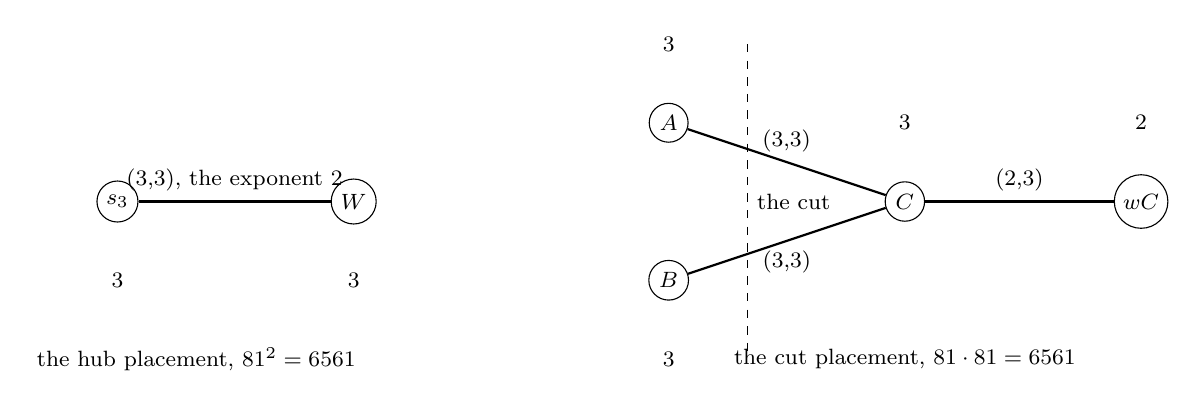
\begin{tikzpicture}[every node/.style={font=\footnotesize}]
\node[circle,draw,inner sep=2pt] (h) at (0,0) {$s_3$}; \node at (0,-1) {$3$};
\node[circle,draw,inner sep=2pt] (w) at (3,0) {$W$}; \node at (3,-1) {$3$};
\draw[thick] (h) -- node[above] {(3,3), the exponent 2} (w);
\node at (1,-2) {the hub placement, $81^2 = 6561$};
\node[circle,draw,inner sep=2pt] (a) at (7,1) {$A$}; \node at (7,2) {$3$};
\node[circle,draw,inner sep=2pt] (b) at (7,-1) {$B$}; \node at (7,-2) {$3$};
\node[circle,draw,inner sep=2pt] (c) at (10,0) {$C$}; \node at (10,1) {$3$};
\node[circle,draw,inner sep=2pt] (d) at (13,0) {$wC$}; \node at (13,1) {$2$};
\draw[thick] (a) -- node[above] {(3,3)} (c); \draw[thick] (b) -- node[below] {(3,3)} (c); \draw[thick] (c) -- node[above] {(2,3)} (d);
\draw[dashed] (8,2) -- node[right] {the cut} (8,-2);
\node at (10,-2) {the cut placement, $81\cdot 81 = 6561$};
\end{tikzpicture}
\caption{The one register at its two placements. At the hub the W word attaches at the site $s_3$ of dimension 3 by one (3,3) link read to the exponent 2. At the horizon the cut severs the two dark (3,3) links from $A$ and $B$ to the star site $C$, beside the (2,3) read tether to the dock $wC$; the product of the two wholes is the same cell.}
\end{figure}
\section{The abundances and the rate at the horizon}\label{mod:X-3-D543792-abrh-t1}
\begin{chtheorem}[The abundances and the rate at the horizon]\label{box:X-3-D543792-abrh-t1:1}
The shares of the termination census are exact rationals at every rung of the horizon web and the growth per tick is an exact element at every step, with the depth-of-the-universe open result an instance at the budget rung and the horizon web re-met at every rung at the kind under the depth rule: at the reading adopted the horizon web at rung 0 is the universe web of 444 sites, 551 links, 27 components and 36 bodies, at rung 1 the 792 webs of its first wave and at rung 2 the 37274 webs of its cut wave, a carried stretch at the rung the budget names, the tick along the parent column equal to the printed wave at 38067 of 38067 and the kind under the depth rule equal to the depth-rule entry at 38066 of 38066 webs, the join kind at 31 webs; the dock-free share at the components pooled reads 26 over 27, 19994 over 20791 and $233\,459$ over $243\,015$ at the count, the charged share 13 over 27, 10218 over 20791 and 79959 over $162\,010$, the bright share 4 over 27, 3178 over 20791 and 16169 over 97206, every one an exact rational compared with nothing; the growth per tick is an exact element at every step, the register at the rank face falling by $2^{2609}\cdot 3^{471}$ over the 792 steps of rung 1 and by $2^{127\,396}\cdot 3^{21350}$ over the 37274 steps of rung 2, the register sum down by 6631 and by $318\,842$; the processed count of the cut wave at the growth table of the horizon-depth entry, 45 against 46 distinct parents, is printed beside, and the uncapped-genre reading parts at rung 1 at the genre (2,3).
\end{chtheorem}
\chstanding{theorem}
\chdeps{Definitions 1.1 to 1.6, Theorems 99.1 and 99.2, Open results 99.3 and 99.4, Theorem 99.5 and Open result 99.6, Theorems 105.1 and 105.2, Open results 105.3 to 105.5 and Theorem 105.6 and Open results 245.1 and 245.2, Theorem 245.3, Open results 245.4 to 245.8 and Theorem 245.9}{no theorem beyond it at this release}
The universe web is parsed from the hand-off and the recorded webs of its saturation are read from the state files at every rung the budget reaches, the shares of the termination census are taken at the bodies pooled at each rung at two census readings and two weightings, and the growth per tick is read at every step at three register faces and by genre. The abundances at the horizon are exact at every recorded rung and the rate is an exact register decrease under the removing moves, the horizon web re-met at every rung at the kind under the depth rule. The horizon, the depth and the saturation stand at their own chapters.
\begin{chbridge}
In cosmology the abundances of the species are fixed at an epoch by the expansion rate and the reaction rates, the primordial abundances following from the first minutes and the expansion rate from the content, and both are measured \cite{Alpher1948,Hubble1929,Friedmann1922}. The correspondence is by name.
\end{chbridge}
\begin{chproof}[exhaustive census with its exact part]
\textit{The premises.} The axiom and the six definitions of Section~\ref{mod:FRAMEWORK}, definitions. The horizon at every rung of Section~\ref{mod:X-3-horizon-at-every-rung-and-the-horizon-web-as-a-seeded-saturation}, a theorem. The depth as the growth order and the termination wave of Section~\ref{mod:X-4-depth-the-growth-order-and-the-termination-wave}, open results. The saturation with its seeds, waves and termination of Section~\ref{mod:I-5-saturation-in-one-figure-seeds-waves-termination-sinks}, a theorem. The chain from the axiom to this result is five chapters deep.

\textit{The census.} The set counted is the recorded webs of the saturation of the horizon web at the reading adopted, the universe web at rung 0 with the genres 85, 34, 229, 134, 67 and 2 and the 792 webs of rung 1 and the 37274 webs of rung 2, 38067 webs in all, and the 35755 of the reading beside. The property tested at every web is its tick along the parent column at one move per step, equal to the printed wave at 38067 of 38067, and its kind under the depth rule equal to the depth-rule entry at 38066 of 38066. The shares at a rung are taken at the bodies of the webs recorded at the rung pooled, the components of the webs, by the census rule of the termination theorem, the membership vector over the six genres: at the count the dock-free share reads 26 over 27 at the 27 bodies of rung 0, 19994 over 20791 at the 20791 bodies of rung 1 and $233\,459$ over $243\,015$ at the $972\,060$ bodies of rung 2, at the unit weights summed the dock-free share reads 806 over 829 at rung 0; the smallest case is rung 0, 27 components of which 26 carry no dock, worked at the figure, the one dock the open dock of the universe web. The growth per tick at every step is the increase of the membership vector by genre and of the register at the three faces, defined at 792 of 792 and 37274 of 37274 steps; summed over rung 1 the net growth by genre reads $-670$, $+419$, $-2214$, $+71$, $-542$, $-72$ with the rank face $-2609$ at 2 and $-471$ at 3, and over rung 2 the rank face $-127\,396$ and $-21\,350$, the removing moves of the saturation lowering the registers at every face but the cut face at the prime 2. The depth-of-the-universe open result is an instance at the budget rung 2, and the uncapped-genre reading parts at rung 1 at the genre (2,3). So the rules pinned ahead read face A yes and face B no, the deciding letter re-lettered at zero freedom at the return from the engine readings at a table id mapped at the single-kind ids. The result is certified at the repository.

\textit{The check.} The rungs widened by one, the rung 1 struck, the (3,3) share in place of the dock-free and the (2,4) links struck each move the cells they name with the face standing where pinned, 4 of 4. The controls read the same at 10 of 11, the one that differs a processed count of the cut wave at 45 against 46 distinct parents, named beside and deciding no grade. The result was reproduced by an independent route, two engines of different construction agreeing at every cell with the runs identical beyond the header line.
\chcert{38067}
\end{chproof}
\begin{figure}[h]
\centering
\begin{adjustbox}{max width=\linewidth}\begin{tabular}{rrrl}
\hline
rung & bodies & without a dock & the dock-free share \\
\hline
0 & 27 & 26 & $(27 - 1)/27 = 26/27$ \\
1 & 20791 & 19994 & $19994/20791$ \\
\hline
\end{tabular}\end{adjustbox}
\caption{The smallest case, rung 0: 27 components of which 26 carry no dock, the one dock the open dock of the universe web; rung 1 beside.}
\end{figure}
\par\medskip\noindent{\itshape The horizon placed, the next chapter reads the depth beneath it.}\label{narr:close:10-3}\par
\section{Depth: the growth order and the termination wave}\label{mod:X-4-depth-the-growth-order-and-the-termination-wave}
\chdesig{6-4}{10-4}{X-4-depth-the-growth-order-and-the-termination-wave}{X-4-D544119-w-pwcd}
\label{narr:open:10-4}Theorem~105.1 reads depth as passage length, Theorem~105.2 the conservation of the depth fraction, Theorem~105.6 the depth independence at the sinks, and the open results Open result~105.3, Open result~105.4 and Open result~105.5 state the growth order, the termination wave and the depth at the deepest sink.
\begin{chconditional}[Depth as passage length]\label{box:X-4-depth-the-growth-order-and-the-termination-wave:1}
Conditional on the results this entry rests on, each at its own standing. The depth of a read is its passage length under the construction adopted, the passage extended beyond the open dock by a new read pair to a fresh frame at every step, the step along the tether forced by the passage parents, the depth-law cells the same under both genre faces; the theorem holds under that construction as a hypothesis and under the (2,3) genre face at the qubit far ends.
\end{chconditional}
\chstanding{conditional theorem}
\chdeps{Definitions 1.1 to 1.6, Theorems 18.1 to 18.4 and Open results 18.5 and 18.6, Open results 241.1 and 241.2, Theorems 241.3 and 241.4 and Open results 241.5 to 241.7 and Open results 245.1 and 245.2, Theorem 245.3, Open results 245.4 to 245.8 and Theorem 245.9}{the theorems of Chapters 1-4, 4-1, 5-15, 6-3 to 6-4, 6-7a}
\begin{chconditional}[Depth fraction conservation]\label{box:X-4-depth-the-growth-order-and-the-termination-wave:2}
Conditional on the results this entry rests on, each at its own standing. The ten readouts under one depth step keep their register fraction, the numerator and the denominator scaling together, while the register count moves by the whole register, the same under the cut rung and the step down; the conservation is an identity given the step and the identity carry of the readout on the free rung, two premises typed by no result, and not a law of the axiom.
\end{chconditional}
\chstanding{conditional theorem}
\chdeps{Definitions 1.1 to 1.6, Theorems 18.1 to 18.4 and Open results 18.5 and 18.6, Open results 241.1 and 241.2, Theorems 241.3 and 241.4 and Open results 241.5 to 241.7 and Open results 245.1 and 245.2, Theorem 245.3, Open results 245.4 to 245.8 and Theorem 245.9}{the theorems of Chapters 1-4, 4-1, 5-15, 6-3 to 6-4, 6-7a}
\begin{chwall}[Depth: the growth order and the termination wave]\label{box:X-4-depth-the-growth-order-and-the-termination-wave:3}
The exponents at the valence face and at the cap face are the readable spare of the universe web at the two bounds, re-derived from the hand-off and re-met, the docking-lemma count that exponent computed once more; but no result fixes the attachment site, so the depth of the horizon read is not fixed. Face A, at least one candidate reading of the attachment site equal to the exponent the derived objects carry, is met. The docking-lemma face iterated to its saturation counts sixty-three at the valence face and four hundred and thirty-two at the cap face, equal to the exponents at every derived cell. Face B, the derivation fixing no one count, is met too, and the parting is named. The three readings of the attachment site give three results, zero and one at the closure-site face, unbounded at the open-end face and sixty-three and four hundred and thirty-two at the docking-lemma face, and the face at which the horizon register is read is fixed by no result, so the depth stands here as a reading carried.
\end{chwall}
\chstanding{open result}
\chdeps{Definitions 1.1 to 1.6, Theorems 18.1 to 18.4 and Open results 18.5 and 18.6, Open results 241.1 and 241.2, Theorems 241.3 and 241.4 and Open results 241.5 to 241.7 and Open results 245.1 and 245.2, Theorem 245.3, Open results 245.4 to 245.8 and Theorem 245.9}{the theorems of Chapters 1-4, 4-1, 5-15, 6-3 to 6-4, 6-7a}
\begin{chwall}[Depth as the growth order of the closure]\label{box:X-4-depth-the-growth-order-and-the-termination-wave:4}
The growth order of the closure is re-met cell for cell and equals the depth coordinate at some readings and not at others, and the horizon count is not a function of the growth order at any closure.
\end{chwall}
\chstanding{open result}
\chdeps{Definitions 1.1 to 1.6, Theorems 18.1 to 18.4 and Open results 18.5 and 18.6, Open results 241.1 and 241.2, Theorems 241.3 and 241.4 and Open results 241.5 to 241.7 and Open results 245.1 and 245.2, Theorem 245.3, Open results 245.4 to 245.8 and Theorem 245.9}{the theorems of Chapters 1-4, 4-1, 5-15, 6-3 to 6-4, 6-7a}
\begin{chwall}[The depth at the deepest sink]\label{box:X-4-depth-the-growth-order-and-the-termination-wave:5}
The depth at the deepest sink is bounded below by the cut wave and fixed by no sink: the deepest sink of the site-bounded closure lies at the cut wave and that of the clean twin at its own, the horizon web is a sink of neither, so the depth is at least four at the first closure and at least five at the twin.
\end{chwall}
\chstanding{open result}
\chdeps{Definitions 1.1 to 1.6, Theorems 18.1 to 18.4 and Open results 18.5 and 18.6, Open results 241.1 and 241.2, Theorems 241.3 and 241.4 and Open results 241.5 to 241.7 and Open results 245.1 and 245.2, Theorem 245.3, Open results 245.4 to 245.8 and Theorem 245.9}{the theorems of Chapters 1-4, 4-1, 5-15, 6-3 to 6-4, 6-7a}
\begin{chconditional}[The depth independence at the sinks]\label{box:X-4-depth-the-growth-order-and-the-termination-wave:6}
Conditional on the results this entry rests on, among them the depth at the deepest sink, each at its own standing. The sink status of every particle web is a function of its sites and links alone: the sink letters re-derived at the stop condition equal the letters the closures typed at every web, no pairing-move edge leaves a parent typed as a sink, and no web changes its sink status with the wave or the cap, the depth part of the bound word dissolved at the sinks.
\end{chconditional}
\chstanding{conditional theorem}
\chdeps{Definitions 1.1 to 1.6, Theorems 18.1 to 18.4 and Open results 18.5 and 18.6, Open results 241.1 and 241.2, Theorems 241.3 and 241.4 and Open results 241.5 to 241.7 and Open results 245.1 and 245.2, Theorem 245.3, Open results 245.4 to 245.8 and Theorem 245.9}{the theorems of Chapters 1-4, 4-1, 5-15, 6-3 to 6-4, 6-7a}
The passage of a read is extended step by step beyond the open dock and its length compared with the depth-law cells under both genre faces. Every readout is carried through one depth step by the distributive law of the trace over a tensor product and the fraction and the count read at the free rung, the cut rung and the step down. The sink letters are re-derived from the sites and links at the stop condition and compared with the letters the closures typed. The three open questions each read the depth and find it fixed by no result. The depth of the horizon read is fixed by no result at the attachment site, the depth coordinate equals the growth order at some readings only, and the depth at the deepest sink is a bound, the termination wave of the horizon web standing at the horizon chapter as a lower bound.
\begin{chbridge}
Two terms of this chapter stand beyond the framework, each defined at its first use, \rosetta{the register tower}{a tower of Hilbert spaces of growing dimension} and \rosetta{the depth metric}{a metric on a lattice}. The correspondence is by name.
\end{chbridge}
\begin{chproof}[finite computation with its census and its exact part]
\textit{The premises.} The axiom and the six definitions of Section~\ref{mod:FRAMEWORK}, definitions. The Born count of Section~\ref{mod:I-3-records-reads-and-the-born-count-the-gain-lemma}, a theorem. The moves of Section~\ref{mod:I-4-moves-in-one-table}, definitions. The saturation of Section~\ref{mod:I-5-saturation-in-one-figure-seeds-waves-termination-sinks}, a theorem. The depth scale at the register tower, the horizon at every rung, the horizon register face at the closure, the cosmological term at the depth exponent and the horizon rung count from saturation, theorems. The universe web, a material by hash. The chain from the axiom to this result is five chapters deep.

\textit{The exact part: the readable spare at one face.} The universe web derived has 444 sites and 551 links with 54 sites of degree one and the one open dock on its tether to the closure site of dimension three at degree three. The readable spare at a bound is the count of the readable spare directions over the sites admitted at that bound. From the sites of dimension two and three admitted at the valence bound, by summation, we obtain
\begin{equation} \adjustbox{max width=\dimexpr\linewidth-3em\relax}{$\displaystyle \begin{gathered} 63 = 51 + 12\quad\text{over 60 sites at the valence face}, \\ 432 = 293 + 139\quad\text{over 369 sites at the cap face}, \end{gathered}$} \end{equation}
listed at the figure, and these are the exponents the derived objects carry at every one of 16 derived cells at each face, re-met. The smallest instance is the one-link model, whose docking-lemma count is $3$ at the valence face and $5$ at the cap face (and $1$ and $2$ at the closure-site face), checked by hand.

\textit{The finite computation.} The input objects are the three readings of the attachment site of the horizon result at the library and at the one-link model. The enumeration rule iterates each reading to its first refusal or its saturation at each bound. The closure-site face, the tether duplicated, gives $0$ at the valence face and $1$ at the cap face to its first refusal. The open-end face, the chain grown at the open end, is unbounded at both faces, admitted at every rung to five hundred. The docking-lemma face, iterated to the saturation with the walk stopped at every readable site at both orders, gives $63$ and $432$, with the mixed faces of the tower $190$ and $305$, the count face $6$ and the order depth $1$ beside, and the un-joined library $81$ and $459$. The test applied is equality with the derived exponent. The docking-lemma count equals it at both faces, because it is that exponent, the saturation count, computed once more. The three objects at it (the ladder object, the whole register to the depth, the tower object, the cut multiplied by it, and the cosmological term, one over the ladder) are exact and equal to the derived objects at 101 of 101 re-meets. The second test, whether the derivation fixes one count, reads no. The three readings give three results and no derived result fixes the attachment site.

\textit{The census.} The set counted is the derived cells carrying the exponent across the entries, 16 at each face. The property tested is equality with the readable spare re-derived from the hand-off, 16 of 16 and 16 of 16, each typed a count of the construction, and the identification of that count with the depth exponent of the horizon read typed a reading carried. The bounds at both faces (the site bound $129$ and $1165$, the free-direction bound $63$ and $507$, the closure saturated at the first and strict at the second) equal the derived cells. The sink status of every particle web, beside, is a function of its sites and links alone. The sink letters re-derived at the stop condition equal the letters the closures typed at every web.

\textit{The check.} Taking another reading of the attachment site, another bound, another order of the walk and another register each move the count they name. Striking the text moves every cell. The result was reproduced by an independent route, two engines of different construction agreeing at every cell at both runs, with the consumed files at 35 of 35 hashes and the six registers of the depth-scale result at 6 of 6 as the controls.
\chcert{101}
\end{chproof}
\begin{figure}[h]
\centering
\begin{adjustbox}{max width=\linewidth}\begin{tabular}{lllll}
\hline
face & sites admitted & spare at the qubit sites & spare at the qutrit sites & the exponent \\
\hline
the valence face & 60 & 51 & 12 & 63 \\
the cap face & 369 & 293 & 139 & 432 \\
\hline
\end{tabular}\end{adjustbox}
\caption{The readable spare of the universe web at the two bounds. At the valence face sixty-three over sixty sites and at the cap face four hundred and thirty-two over three hundred and sixty-nine sites, the exponents the derived objects carry, re-derived from the hand-off.}
\end{figure}
\section{The depth and the cap count at a larger budget}\label{mod:X-4-D540569-w-tlgc}
\begin{chwall}[The depth and the cap count at a larger budget]\label{box:X-4-D540569-w-tlgc:1}
Face A, the valence census of the universe web terminating at an exact wave at which a depth cell of the depth entries compares equal or the bound is attained, is met at no piece. Face B, the census terminating at an exact wave beneath the lower bound or beneath the depth at every reading of open, is met at no piece either. At a piece budget widened from 40 to 240 the valence census resumed from the last state of the widened census stays unterminated within the larger budget: the same three links that were open at the carried stretch stay open at every one of the 200 pieces beyond it, 548 of 551 links are capped by wave 1 and the changes per wave read 63 then 0, wave 2 is run to the 83rd of its 792 frontier webs with 84680 webs recorded, so the larger budget is exhausted first, the terminating wave stays a lower bound 1, and the comparison with the depth, a lower bound 3 fixed by no entry, stays undecided at a budget a factor of six over the widened one; the key, shared and key-and-shared readings are re-met at their terminating waves 0, 1 and 1, the depth exceeding them by at least 3, 2 and 2, and the register growth at the capped links reads 16986 at wave 1 and 0 at wave 2.
\end{chwall}
\chstanding{open result}
\chdeps{Definitions 1.1 to 1.6, Theorems 99.1 and 99.2, Open results 99.3 and 99.4, Theorem 99.5 and Open result 99.6, Theorems 105.1 and 105.2, Open results 105.3 to 105.5 and Theorem 105.6 and Open results 245.1 and 245.2, Theorem 245.3, Open results 245.4 to 245.8 and Theorem 245.9}{no theorem beyond it at this release}
The saturation of the universe web is resumed from the last state of the widened run and carried 200 pieces beyond it at the reading of open that keeps every end with spare valence open, the carried stretch re-derived equal to the widened run at every state and the three positions of the return of that run, the 96th, 99th and 101st frontier webs, lying beyond the 83rd reached. The result is an instrument of the waves run, a budget letter deciding neither face, and the same census at a still larger budget is the one further path recorded. The depth as a growth order and the termination wave stand at their own chapters.
\begin{chbridge}
A cosmological horizon in the literature is the boundary of the region a signal can reach in a finite span, and the question whether an expanding region closes or grows without bound is answered by the sign of its curvature and the content it carries \cite{Friedmann1922,HawkingEllis1973}. The correspondence is by name.
\end{chbridge}
\begin{chproof}[finite computation with its census]
\textit{The premises.} The axiom and the six definitions of Section~\ref{mod:FRAMEWORK}, definitions. The saturation with its seeds, waves and termination of Section~\ref{mod:I-5-saturation-in-one-figure-seeds-waves-termination-sinks}, definitions and a theorem. The depth as the growth order and the termination wave of Section~\ref{mod:X-4-depth-the-growth-order-and-the-termination-wave}, open results. The horizon web at the cap of Section~\ref{mod:X-3-horizon-at-every-rung-and-the-horizon-web-as-a-seeded-saturation}, an open result. The chain from the axiom to this result is five chapters deep.

\textit{The procedure.} The input is the last state of the widened run, the universe web of 444 sites and 551 links seeded at wave 0 with 497 links at their cap and 54 uncapped, resumed at the valence reading, under which an end stays open while it carries spare valence. A piece processes frontier webs in the fixed order, admitting at most 1200 canonical candidates per piece as the depth run and the widened run admitted them, so that the carried stretch is re-met piece for piece; the budget is 240 pieces per chain against 40 at the widened run, the web budget $288\,000$, the wave bound 8 and the leaf bound 4000. The test applied at each wave is the cap status of every link, a link capped once its register reaches the sum of its end sets; the stop rule fires when no link is uncapped. The aggregation is the histogram of first capping waves and the register sum at the capped links per wave.

\textit{The totals.} The carried stretch, the seed state and the 39 pieces of waves 1 and 2 of the widened run, is re-derived equal byte for byte at 160 of 160 states over both engines and both runs, the cut piece re-run whole and equal at every line beyond the budget keys, the 82 captures equal cell for cell. Beyond the carried stretch the 200 new pieces reach the 83rd frontier web of the 792 of wave 2 at the candidate 541, with the webs by wave
\begin{equation}
0:1,\qquad 1:792,\qquad 2:83887,
\end{equation}
84680 webs recorded, the totals over the chain $576\,862$ candidates, $286\,939$ admitted and $1\,018\,276$ removed. The first capping histogram reads 485 at wave 0, 63 at wave 1 and 0 at wave 2, the capped count 485, 548 and 548 and the uncapped count 66, 3 and 3 by wave, so the changes per wave are 63 then 0 and the three links open at the budget are the two hub-to-core pairs of the bodies 1 and 11 at the register 34 and the core-to-star link of the body 14 at the register 23. The register at the capped links grows by genre at wave 1 by
\begin{equation}
252 + 690 + 8772 + 936 + 6336 + 0 = 16986
\end{equation}
over the six genres from $493\,813$ to $510\,799$ and by 0 at wave 2, at two routes equal. The smallest instance is the shared reading at wave 1, re-met here: 54 uncapped links at the seed, every one capped at wave 1, the register growing by $11\,394$, the terminating wave 1; the key reading terminates at wave 0 with 221 capped and 330 fixed uncapped and the key-and-shared reading at wave 1. Against the depth, a lower bound 3 at the raised budget, the terminating waves 0, 1 and 1 fall short by at least 3, 2 and 2 and the valence reading stays undecided, so the rule pinned ahead reads face A no, face B no and the budget letter yes.

\textit{The check.} The seed struck to the one root link, the reversal cut removed, the junction move removed and the text struck each move the cells they name, the census run from the electron web of known depth terminates at its own wave and reads equal at every reading, the positive control, and the carried stretch re-run equals the widened run at 82 of 82 captures. The controls read the same at 17 of 17 beyond the two engine spellings carried as parting by construction, the chain-summing identities re-posed at the cap-wave carried stretch at 4 of 4 among them. The result was reproduced by an independent route, two engines of different construction agreeing at every cell at both runs.
\chcert{84680}
\end{chproof}
\section{The depth rule as the dynamics}\label{mod:X-4-D543100-w-prdd}
\begin{chwall}[The depth rule as the dynamics]\label{box:X-4-D543100-w-prdd:1}
Face A, the growth order of the closure and the termination wave one object under the two moves of the depth rule as the forces open result names them, the evolution at one step per tick with the advance of every settled configuration printed, reads no. Face B reads yes with the first parting named: the growth order counts the acts of the pair ket from the root, 582 attaches at every genre, 432 hub acts adding four sites and 94 joins at equal genres, and the termination wave counts the reverses of the table from the universe web, $31\,412$ reverse cuts, the reverse hub steps and 9 reverse attaches, with the 92 joins within the web, each equal to its own tick count along its parent column at every one of 1113 and 73822 webs, while the two moves of the rule, the hub-forming pairing and the (2,2) join, advance 67 of 1108 closure webs and 31 of 38066 and 31 of 35754 recorded webs; the first parting at the closure is the root qubit docked with a second qubit, the first closure at its first join at the web 2 at order 1 under an attach at the genre (2,2), an advance of neither the rule nor the table, and at the termination wave the web 10 at wave 1 under the reverse attach; under every move of the table at one step per tick the termination wave is one object with the table at every recorded web and the closure parts at the same first web with 186 equal-genre attaches and 432 hub acts of another alphabet. Beside, at the site bound six of the closure without caps, the admission clause of the rule struck: from the six genre links the closure with the two attaches at the equal genres admitted among the twenty-eight moves runs to exhaustion at 589 webs over eleven waves with twenty-five sinks at the move set and reaches six of the catalogued webs, among them the up quark bare and docked, the gluon word and the Higgs word, while the closure with the clause in force runs to exhaustion at 84 webs over eight waves with no sink and reaches five of them, the gluon word never; the ruled closure is contained in the struck at 84 of 84, the sinks part at twenty-five against none and the reached webs at the gluon word, four qutrits over three (3,3) links, twenty-six partings in all, the first a web of four sites at three links reached through the attach at the genre (3,3), present at the struck closure as an open state of the closure without caps and absent at the ruled.
\end{chwall}
\chstanding{open result}
\chdeps{Definitions 1.1 to 1.6, Theorems 105.1 and 105.2, Open results 105.3 to 105.5 and Theorem 105.6, Open results 241.1 and 241.2, Theorems 241.3 and 241.4 and Open results 241.5 to 241.7 and Open results 245.1 and 245.2, Theorem 245.3, Open results 245.4 to 245.8 and Theorem 245.9}{no theorem beyond it at this release}
The two depth open results are transcribed at their cells and re-derived along their parent columns, the depth rule is carried at its move table with its two electromagnetic moves re-met at the forces table, and the advance of every settled configuration is printed step by step under the two moves and under the whole table. The two open results are two alphabets, the acts of the pair ket and the reverses of the table, and one object not. The depth and the move table stand at their own chapters.
\begin{chbridge}
In the literature the dynamics of a system is one rule applied one step per unit of the clock, a Hamiltonian flow or a cellular automaton, and the depth of a configuration is the number of steps from the initial state under that rule \cite{Newton1687,Weinberg1995}. The correspondence is by name.
\end{chbridge}
\begin{chproof}[exhaustive census]
\textit{The premises.} The axiom and the six definitions of Section~\ref{mod:FRAMEWORK}, definitions. The depth as the growth order and the termination wave of Section~\ref{mod:X-4-depth-the-growth-order-and-the-termination-wave}, open results. The moves in one table of Section~\ref{mod:I-4-moves-in-one-table}, definitions. The saturation with its seeds, waves and termination of Section~\ref{mod:I-5-saturation-in-one-figure-seeds-waves-termination-sinks}, a theorem. The chain from the axiom to this result is four chapters deep.

\textit{The census.} The set counted is the settled configurations of the two open results: the five closures of the pair ket at 1113 webs, with the orders by closure 1 then 3 at the first, 1, 3, 1 at the second, 1, 5, 18, 79, 300, 101 at the third, 1, 5, 20, 91, 371, 16 at the fourth and four webs at every order from one to twenty-three with three at twenty-four at the fifth, and the 73822 recorded webs of the saturation of the universe web at its two readings, 38067 at the first with the webs by wave 1, 792 and 37274 and 35755 at the second with 1, 738 and 35016. The order of every web and the wave of every web are re-derived along the parent column, a root at 0 and a child one beyond its parent, equal to the printed cells at 1113 of 1113 and 73822 of 73822. The rule is carried at its cells: the move table of 28 moves, 10 adding, 10 removing and 8 keeping the site count, closed under the inverse at 14 of 14 pairs, the move-tick map zero at 9 of 9 moves and the depth increment zero at 8 of 8, and the two moves the forces open result names at the electromagnetic, the hub-forming pairing adding two sites at 16 edges of the sinks and the (2,2) join keeping the site count at 31325 edges. The property tested at every configuration is the move or act by which it advances from its parent and its kind under the rule, the two moves against the rest. At the closure the 1108 advances read 582 attaches, 179 at (2,2), 194 at (2,3), 195 at (2,4), 7 at (3,3) and 7 at (3,4), 432 hub acts at the site delta 4 and 94 joins, 67 at (2,2), 23 at (3,3) and 4 at (4,4); at the termination wave the 38066 advances of the first reading read 31 (2,2) joins, 61 (3,3) joins, 1866 reverse (3,3) joins, 9 reverse attaches, $31\,412$ reverse cuts, 1047 reverse hub pairings, 2544 reverse hub doublings, 323 reverse hub returns and 773 reverse hub steps at a kept leg, and the 35754 of the second reading alike with 31 joins. Under the two moves of the rule the advances equal at
\begin{equation}
67 \text{ of } 1108,\qquad 31 \text{ of } 38066,\qquad 31 \text{ of } 35754,
\end{equation}
the first parting at the closure the web 2 of the first closure at order 1, the root qubit docked with a second qubit under an attach at the genre (2,2), a move neither of the rule nor of the table, and at the termination wave the web 10 at wave 1 under the reverse attach, a move of the table and not of the rule; under every move of the table with its inverse the termination wave equals at 38066 of 38066 and 35754 of 35754 and the closure at 922 of 1108 with the same first parting, 186 equal-genre attaches unmapped and the 432 hub acts at the delta 4 against the delta 2 of the hub-forming move. The smallest case is the first closure at its first join, the root at order 0, three webs at order 1, the second of them the first parting.

\textit{The check.} One move of the rule struck lets the advances under the rule fall to 0 at every open result, two steps per tick part the tick from the order and the wave at every web beyond the roots and the seeds, the step reversed moves the deciding cells, and every configuration taken as already terminated moves the tick to the root value at every web, 4 of 4 as pinned. The controls read the same at 11 of 11. The result was reproduced by an independent route, two engines of different construction agreeing at every cell with the runs byte-identical.
\chcert{73822}
\end{chproof}
\begin{figure}[htbp]\centering
\setlength{\unitlength}{1mm}
\begin{picture}(160,74)(0,0)
\put(0,61){\makebox(52,8){\scriptsize the tick, the attach at (2,2), tick}}
\put(58,61){\framebox(7,7){\scriptsize 2}}
\put(78,61){\makebox(10,7){\scriptsize to}}
\put(92,61){\framebox(7,7){\scriptsize 2}}
\put(108,61){\framebox(7,7){\scriptsize 2}}
\qbezier(99,64)(103,64)(108,64)
\put(96,56){\makebox(20,4){\tiny the site 2 inserted}}
\put(118,61){\makebox(42,7){\tiny at the closure alphabet alone, 1 site and 1 link added; at no row of the table}}
\put(0,45){\makebox(52,8){\scriptsize the carrier, the attach at (2,3), carrier}}
\put(58,45){\framebox(7,7){\scriptsize 2}}
\put(78,45){\makebox(10,7){\scriptsize to}}
\put(92,45){\framebox(7,7){\scriptsize 2}}
\put(108,45){\framebox(7,7){\scriptsize 3}}
\qbezier(99,48)(103,48)(108,48)
\put(96,40){\makebox(20,4){\tiny the site 3 inserted}}
\put(118,45){\makebox(42,7){\tiny A1 adds 1 site; A1I strikes it (-1)}}
\put(0,29){\makebox(52,8){\scriptsize the vacuum, the attach at (2,4) with the hub-forming move, vacuum}}
\put(58,29){\framebox(7,7){\scriptsize 2}}
\put(78,29){\makebox(10,7){\scriptsize to}}
\put(92,29){\framebox(7,7){\scriptsize 2}}
\put(108,29){\framebox(7,7){\scriptsize 4}}
\qbezier(99,32)(103,32)(108,32)
\put(96,24){\makebox(20,4){\tiny the site 4 inserted}}
\put(118,29){\makebox(42,7){\tiny A2 adds 1 site, HF adds 2 sites, the hub act 4 sites and 5 links}}
\put(0,13){\makebox(52,8){\scriptsize the closure, the join at (2,2), closure}}
\put(58,13){\framebox(7,7){\scriptsize 2}}
\put(70,13){\framebox(7,7){\scriptsize 2}}
\put(78,13){\makebox(10,7){\scriptsize to}}
\put(92,13){\framebox(7,7){\scriptsize 2}}
\put(108,13){\framebox(7,7){\scriptsize 2}}
\qbezier(99,16)(103,16)(108,16)
\put(96,8){\makebox(20,4){\tiny the link (2,2) inserted}}
\put(118,13){\makebox(42,7){\tiny J2 keeps the site count at 0; J2I strikes the link}}
\put(0,0){\makebox(160,5){\scriptsize the closure advances under the four at the recorded reading: the tick 179, the carrier 194, the vacuum 627 (the attach 195 and the hub act 432), the closure 67; the termination wave: the carrier R2 9;R1 9, the closure R2 31;R1 31}}
\end{picture}
\par\smallskip
{\scriptsize\begin{adjustbox}{max width=\linewidth}\begin{tabular}{llllll}
id & the kinds & the site action & the site delta & the class under the two moves & the move of the rule \\ \hline
A1 & attach at (2,3) & adds & 1 & other & the carrier \\
A1I & the reverse attach at (2,3) & removes & -1 & other & the carrier, the inverse \\
A2 & attach at (2,4) & adds & 1 & other & the vacuum, the attach \\
A2I & the reverse attach at (2,4) & removes & -1 & other & the vacuum, the inverse \\
HF & hub-forming & adds & 2 & hf & the vacuum, the hub-forming move \\
the inverse of HF & the reverse hub-forming & removes & -2 & hf & the vacuum, the inverse \\
J2 & join within at (2,2), join across at (2,2) & keeps & 0 & j2 & the closure \\
J2I & the reverse join within at (2,2), the reverse join across at (2,2) & keeps & 0 & j2 & the closure, the inverse \\
the hub step forward & hub step p, hub step with the kept leg, hub step r & adds & 4,3,4 & other & the hub step family beside \\
the hub step reverse & the reverse hub step p, the reverse hub step with the kept leg, the reverse hub step r & removes & -4,-3,-4 & other & the hub step family, the inverse \\
\hline
\multicolumn{6}{l}{the table at 28 moves closed under the inverse rule at 14 of 14 pairs; the electromagnetic carried by HF;J2 at the genre (2,2), HF at 16 edges and J2 at 31325 edges} \\
\end{tabular}\end{adjustbox}}
\caption{The recorded move table drawn as the rule: the table at 28 moves closed under the inverse rule at 14 of 14 pairs, its two moves at the electromagnetic the hub-forming pairing HF and the (2,2) join J2, both at the carrier genre (2,2); the four moves of the depth rule, the tick, the carrier, the vacuum and the closure, located at the table and at the act alphabet of the recorded closure: the attach at (2,2) at no row of the table and at the closure alphabet at 179 advances, the attach at (2,3) at the table at A1 and at the closure at 194 advances, the (2,4) hub act at the table at the attach A2 and at the hub-forming move HF and at the closure at 195 attaches at (2,4) and 432 hub acts, the join at the table at J2 and at 67 closure joins; the electromagnetic carried by two move classes, HF at 16 edges and J2 at 31325 edges of the recorded sinks (the photon of the literature named for the board). Each neighbourhood is drawn at the qubit end, the site the move inserts at its dimension beside the link it makes, the inverse striking them; the kinds of the table are spelled in words.}\label{fig:X-4-D543100-move-rule}
\end{figure}
\section{The seven depth readings as one object}\label{mod:X-4-D543126-w-svdq}
\begin{chwall}[The seven depth readings as one object]\label{box:X-4-D543126-w-svdq:1}
Face A, every one of the seven depth readings one object with the serial (2,2) count or its logarithm at the webs the count is carried at, reads no. Face B reads yes with the first parting named: at the universe web the count along the chain is 1 and its logarithm 1, the tower $24\cdot 36$ over the origin 24 to the base 36, and the depth-web open result reads its chain length 0 there, the horizon-closure open result its ten candidates, 0, unbounded, 63, 1, unbounded, 432, 190, 305, 45 and 1, the deepest-sink open result its bounds 4 and 5 and the register-tower open result its bounds 3, 3, 4 and 5; at the lepton webs the count is 1 at every one and the mass-ladder open result reads its index 0, 1, 2 and its momentum 1, 2, 3; the growth-order open result and the transfer-count open result name no web the count is carried at; the first parting is the depth-web open result, its chain length 0 against the count 1 and the logarithm 1 at the universe web, the whole-web count 85 beside; the open results at one object number 0 of 7, five surviving their parting and two naming no shared web.
\end{chwall}
\chstanding{open result}
\chdeps{Definitions 1.1 to 1.6, Theorems 105.1 and 105.2, Open results 105.3 to 105.5 and Theorem 105.6 and Theorems 113.1 and 113.2}{no theorem beyond it at this release}
The seven depth open results are transcribed at their deciding cells, the serial (2,2) count and its logarithm are read at every chain state of the depth-metric open result, and every depth cell at a web the count is carried at is compared with the count and with the logarithm. Seven vocabularies of depth are not one object at the (2,2) reading. The depth and the register tower stand at their own chapters.
\begin{chbridge}
In the literature the dimension of space is one number, read alike from the growth of a ball, from the spectrum of the Laplacian, from the scaling of an entropy and from the number of independent directions, every reading agreeing on three \cite{Wald1984,HawkingEllis1973}. The correspondence is by name.
\end{chbridge}
\begin{chproof}[finite computation]
\textit{The premises.} The axiom and the six definitions of Section~\ref{mod:FRAMEWORK}, definitions. The depth as the growth order and the termination wave of Section~\ref{mod:X-4-depth-the-growth-order-and-the-termination-wave}, open results. The register tower of Section~\ref{mod:X-5-register-tower-and-the-metric}, a theorem. The depth metric of the chapter titled The (2,2) genre, the pair ket, the serial link and the increment (chapter~\ref{mod:X-0-D540399-the-two-two-census-at-every-placement}, among the instruments), at its standing. The chain from the axiom to this result is five chapters deep.

\textit{The procedure.} The seven open results are transcribed at their deciding and parting cells by locator, every one a face-B cell at an open result, 51 depth cells in all: the depth-web open result at the chain length 0 at the universe web and its first refusal at k 1, the growth-order open result at the growth order of its closure webs, the transfer-count open result at the wave of its closure webs, the horizon-closure open result at ten candidates of the universe web, the deepest-sink open result at the bounds 4 and 5, the mass-ladder open result at the index and the momentum of the three leptons, and the register-tower open result at the bounds 3, 3, 4 and 5. The serial (2,2) count along the chain run is read at 40 chain states, 1 at the hub-unit pairs of the electron, the muon, the tau, the neutron and the universe web, 0 at the dock chains of the proton and the photon word, the count metric equal to 96 multiplied by the count at 80 of 80, and the logarithm of the tower over the origin 24 to the base 36 is re-derived at every chain state by two routes, exact at 40 of 40 and equal to the count. The rule pinned ahead reads a deciding depth cell equal if it equals the count or the logarithm at its web, an open result one object if every such cell is equal and it has one, no shared web at none, and parting survives otherwise.

\textit{The totals.} At the universe web the count is 1 and the logarithm
\begin{equation}
\log_{36}\frac{24\cdot 36}{24} = 1,
\end{equation}
the smallest instance worked on the page, the whole-web count 85 beside. Against them the depth-web open result reads 0, equal at 0 of its 2 deciding cells; the horizon-closure open result reads its ten candidates, equal at 2 of 10, the closure-site face 1 at the cap bound and the order 1; the deepest-sink open result reads 4, the bound 4 against 1 and 1; the register-tower open result reads 3, the bound 3 against 1 and 1; at the lepton webs the mass-ladder open result reads the index 0, 1, 2 and the momentum 1, 2, 3 against the count 1, equal at 2 of 6; the growth-order open result at the root and the docked bodies and the transfer-count open result at its closure webs name no web the count is carried at. So the open results at one object number 0 of 7, five at parting survives and two at no shared web, face A reads no and face B reads yes with the first parting the depth-web open result. The comparison of every depth cell is printed at 35 cells at the universe web and the lepton webs at k 0 with the k beyond beside.

\textit{The check.} The universe web struck from the comparison webs moves four open results to no shared web and the first parting to the mass-ladder open result, the (2,3) count in place of the (2,2) moves two open results to one object under the struck count, the shifted origin moves the depth-web open result to one object under the struck logarithm, the text struck excludes the run, and the web with no insertion moves the counts at k 1 to 3, 5 of 5 as pinned. The controls read the same at 16 of 16, among them the count-metric theorem, the depth-metric open result, the seven open results at their partings and the web identities at 10 of 10. The result was reproduced by an independent route, two engines of different construction agreeing at every cell at both runs.
\chcert{51}
\end{chproof}
\section{Open as the depth far end}\label{mod:X-4-D543900-w-opdf}
\begin{chwall}[Open as the depth far end]\label{box:X-4-D543900-w-opdf:1}
Face A, one of the two definitions of open, the first opening the smaller end or the derived opening the larger, equal to the depth-far rule at every unequal link of every settled web with the far end named at every link, reads no. Face B reads yes with the first link named: at the arrow of a link, the chain of the link read from its tail to its head, settled at every link of the web table and carried to the universe web, the far end is the smaller end, the one the first definition opens, at 3852 of the 4642 unequal links of every settled web and the larger end, the one the derived definition opens, at 248, with no far end at 542, the 295 unequal links of the sinks beyond wave zero whose link lists are not settled and 247 settled links with no arrow, by genre 384 against 48 at (2,3), 2809 against 7 at (2,4) and 659 against 193 at (3,4), so the one-definition reading reads mixed; the first link where neither holds is the second link of the first web of the table, from its hub F to its leg f1 at the genre (4,2), whose far end f1 is the smaller, the first definition having parted at the first link from the core Q to the hub F at (3,4) whose far end F is the larger; along the chain runs of the two-metrics open result the far end is the derived open end at 8 of 8 unequal run links, under the tree distance from the depth-zero site it names the first definition at 1001, the derived at 386 and no end at 2960 links of equal depth, and under the serial (2,2) count read as a depth it names no end at any unequal link; the two parents part at the photon word chain link.
\end{chwall}
\chstanding{open result}
\chdeps{Definitions 1.1 to 1.6, Theorems 9.1 to 9.7 and Open result 9.8, Theorems 28.1 and 28.2, Open results 28.3 and 28.4 and Theorem 28.5 and Theorems 105.1 and 105.2, Open results 105.3 to 105.5 and Theorem 105.6}{no theorem beyond it at this release}
Every unequal link of every settled web is typed under the two definitions of open from the dimensions alone, the two being mirrors, and the depth-far rule, the end of a link away from the depth-zero end of its chain, is read at four readings at every link and compared with the two definitions. The depth-far end at the arrow is a third reading of open, coinciding with the first definition where the hub stands first and with the derived where the core or the dock qubit stands first, so the depth fixes neither definition at every link. The link, the read and the depth stand at their own chapters.
\begin{chbridge}
In relativity the forward end of a world line is fixed by the arrow of the proper clock along it, and which of two events follows the other is decided by the orientation of the light cone, a convention at no point and a fact along every world line \cite{Minkowski1908,HawkingEllis1973}. The correspondence is by name.
\end{chbridge}
\begin{chproof}[exhaustive census with its exact part]
\textit{The premises.} The axiom and the six definitions of Section~\ref{mod:FRAMEWORK}, definitions. The link and its six genres of Section~\ref{mod:I-2-link-and-its-six-genres}, definitions. The read at a register of Section~\ref{mod:I-6-read-at-a-register-the-probe-and-the-measurement}, definitions and theorems. The depth as the growth order and the termination wave of Section~\ref{mod:X-4-depth-the-growth-order-and-the-termination-wave}, open results. The chain from the axiom to this result is four chapters deep.

\textit{The census.} The set counted is the unequal links of every settled web of this result: the 64 webs of the web table, 1691 links of which 930 unequal; the 40 chain states of the two-metrics open result, 2960 unequal links; the eight webs of the definition open results, the universe web with 330 unequal and the seven roster webs with 51; and the 88 terminated sinks of the sinks entry, 371 unequal links; 4642 unequal links in all, 4347 with settled links. The property tested at every link is the far end under the depth-far rule at four readings against the two definitions: the first definition opens an end whose dimension is less than the far dimension and the derived opens an end whose dimension exceeds it, mirrors at 4347 of 4347 settled links, the end letters of the definition open results re-met at 1262 of 1262. At the arrow, the reading adopted, the chain of a link is read from its tail to its head, the arrow equal to the end order of the link line at 1691 of 1691 and carried to the universe web at 551 of 551, with no arrow at the inserted run links, the roster webs and the sinks beyond wave zero: the far end is named at 4100 links and none at 542, and where named it is the smaller end at 3852 and the larger at 248, $3852 + 248 + 542 = 4642$, by genre 384, 48 and 75 at (2,3), 2809, 7 and 98 at (2,4) and 659, 193 and 74 at (3,4). The smallest case is the first web of the table, worked at the figure. At the chain run the far end is the derived open end at 8 of 8 unequal run links and none at 4634; at the tree distance it is the first definition at 1001, the derived at 386 and none at 2960; under the serial (2,2) count no unequal link has a far end; the two parents part at the photon word chain link alone. So the rule pinned ahead reads face A no at the mixed reading and face B yes with the first link named, and the first link where the rule names no end is the entry link of the proton chain. The result is certified at the repository.

\textit{The check.} The arrow reversed exchanges the two letters, 248 and 3852, with the deciding cell standing, the derived re-pointed to the smaller end removes the mirror and reads neither at the larger-end links, and the reading moved to the chain run or to the tree distance moves the census as printed with the deciding cell standing, 4 of 4 as pinned. The controls read the same at 10 of 10, the arrow equal to the end order at 1691 of 1691 among them. The result was reproduced by an independent route, two engines of different construction agreeing at every cell with the runs byte-identical.
\chcert{4642}
\end{chproof}
\begin{figure}[h]
\centering
\begin{adjustbox}{max width=\linewidth}\begin{tabular}{llll}
\hline
link of the first web & end dimensions & the far end & the definition that parts \\
\hline
the core Q to the hub F & 3 and 4 & F, the larger & the first \\
the hub F to the leg f1 & 4 and 2 & f1, the smaller & the derived \\
\hline
\end{tabular}\end{adjustbox}
\caption{The smallest case, the first web of the table: at its first link the far end is the larger, where the first definition parts, and at its second the smaller, where the derived parts; the first link is where neither holds.}
\end{figure}
\section{The depth rule run to the budget at the universe web}\label{mod:X-4-D544065-the-depth-rule-run-to-the-budget-at-the-universe-web}
\begin{chtable}[The depth rule run to the budget at the universe web]\label{box:X-4-D544065-the-depth-rule-run-to-the-budget-at-the-universe-web:1}
At the three rungs the budget reaches at the horizon entry, 1, 792 and 37274 webs by rung with rung 2 a carried stretch, and at the widened-budget open result, 1, 792 and 14087, the three series of the (2,2) web are printed with the continuum statements located: the ball-growth exponent of the (2,2) web as the one-exponent census over the webs, at rung 0 yes 0, no 0, short 1, at rung 1 yes 8, no 8, short 776 and at rung 2 yes 6421, no 336, short 30517; the second difference of the (2,2) count across the web, zero at every pair site at 1 web of rung 0, 776 webs of rung 1 and 30517 webs of rung 2, the value census at rung 2 reading $-1$ at 13664, 0 at $6\,243\,534$, 1 at 12888 and 2 at 388; and the modulation along the rays, the step of the (2,2) count against the parent, at rung 1 reading $-2$ at 7, $-1$ at 664, 0 at 113 and 1 at 8 and at rung 2 $-2$ at 316, $-1$ at 32241, 0 at 4694 and 1 at 23, the ray letters at rung 2 uniform 23, still 3782, varying 33469; the ball-growth open result at one exponent first holds at rung 1 and first fails at rung 1, short at rung 0; the classical-limit open result at its inverse-square form first fails at rung 2 and first holds at no rung, its linear chain form first holding and first failing at rung 2; the wave at the rule adopted first fails at rung 1 and first holds at no rung, and at the period-one reading first holds at rung 1 and first fails at rung 2.
\end{chtable}
\chstanding{instrument}
\chdeps{Definitions 1.1 to 1.6, Theorems 90.1 to 90.4, Theorems 99.1 and 99.2, Open results 99.3 and 99.4, Theorem 99.5 and Open result 99.6 and Theorems 105.1 and 105.2, Open results 105.3 to 105.5 and Theorem 105.6}{no theorem beyond it at this release}
The depth rule is run to the budget at the universe web as an instrument: at every rung the budget reaches the ball-growth exponent of the (2,2) web, the second difference of the (2,2) count and the modulation along the rays are printed from the horizon entry and the widened-budget open result, with the rung at which each continuum statement first holds or fails, every cell exact and compared with nothing. The depth, the horizon and the curvature stand at their own chapters.
\begin{chbridge}
In the continuum the dimension of space is the exponent of the growth of a ball, the Laplacian of a density vanishes where the density is harmonic, and a wave is a modulation of a field along a ray at a fixed period, three statements the literature takes as holding at every point and at every scale \cite{Wald1984,Weinberg1995}. The correspondence is by name.
\end{chbridge}
\begin{chproof}[instrument table]
\textit{The rule that produced the table.} The webs by rung are read from the rungs table of the horizon entry at its reading adopted, 1, 792 and 37274 at the rungs 0, 1 and 2 with rung 2 a carried stretch at the budget, and from the webs table of the widened-budget open result beside, 1, 792 and 14087. At every recorded web the (2,2) web is its pair links, chains and pair sites. The ball-growth exponent is the one-exponent census of the summed ball of the (2,2) web over its orders below saturation, yes where one exponent stands at a settled growth reading, no where it does not and short where the orders carry no step; the second difference is the row-sum-zero operator of the counting face on the (2,2) links applied to the count at every pair site; the modulation is the step of the (2,2) count of a web against its parent along the rays from the seed. The columns of the table below are the series, the rung and the census at the reading adopted.

\begin{center}
\begin{adjustbox}{max width=\linewidth}\begin{tabular}{lll}
\hline
series & rung & the census at the reading adopted \\
\hline
the ball-growth exponent & 0 & yes 0, no 0, short 1 \\
 & 1 & yes 8, no 8, short 776 \\
 & 2 & yes 6421, no 336, short 30517 \\
the second difference zero at every pair site & 0, 1, 2 & 1 of 1, 776 of 792, 30517 of 37274 webs \\
the modulation along the rays & 1 & $-2$ at 7, $-1$ at 664, 0 at 113, 1 at 8 \\
 & 2 & $-2$ at 316, $-1$ at 32241, 0 at 4694, 1 at 23 \\
\hline
\end{tabular}\end{adjustbox}
\end{center}

\textit{The counts of the table.} The pooled summed ball over the webs reads 170 then 340 at rung 0 with its growth readings short, $133\,276$, $266\,576$, $266\,624$ and $266\,640$ at rung 1 and $6\,270\,474$, $12\,554\,224$, $12\,580\,776$ and $12\,593\,664$ at rung 2, its growth readings not fixed; the diameter census at rung 2 reads 1 at 30517, 2 at 336 and 3 at 6421. The value census of the second difference at rung 1 reads $-1$ at 32, 0 at $133\,220$, 1 at 16 and 2 at 8 with the trace census 166 at 7, 168 at 664, 170 at 113 and 172 at 8, and the (2,2) count census at rung 2 reads 83 at 252, 84 at 26869, 85 at 9218, 86 at 912 and 87 at 23. The ray letters at rung 1 read uniform 679, still 113 and varying 0, every ray read from the seed, and the net modulation $-670$ at rung 1 and $-32850$ at rung 2 equals the net (2,2) growth of the horizon entry. The continuum statements fall as the box prints them, the ball-growth open result holding at 8 and failing at 8 of the 792 webs of rung 1 and holding at 6421 and failing at 336 of rung 2, the classical-limit open result failing at every web of rung 2 at its inverse-square form and holding at 3805 and failing at 33469 at its linear chain form, and the wave failing at every web at the rule adopted and holding at 792 of rung 1 and 3805 of rung 2 at the period-one reading; at the reading beside the one-exponent census at rung 2 reads yes 6421, no 90, short 7576. The genre beside read in place of the genre adopted, the first link of the genre struck at every web and the rays reversed each move the cells they name, and a wrong hash excludes the run, 4 of 4 as pinned; the controls read the same at 12 of 12, among them the dark ball of the universe web at every apex equal to the ball-growth open result at the diameter 14 and the radius 1, the (2,2) web of the universe web equal to the nonlinear open result at the operator applied to the count, and the net growth equal to the growth table of the horizon entry. The table was reproduced by an independent route, two engines of different construction agreeing at every cell.
\end{chproof}
\section{The area coefficient as the depth count}\label{mod:X-4-D544091-w-ardc}
\begin{chwall}[The area coefficient as the depth count]\label{box:X-4-D544091-w-ardc:1}
Face A, the area coefficient at every rung of the fixed cut equal to the rung count multiplied by the rung-one coefficient at both readings, reads no. Face B reads yes with the first rung named: at the fixed cut of the horizon web the cut register is one register at every rung, $236\,196$, the logarithm 2 log 2 plus 10 log 3, and the coefficient at rung k, the hidden records over that logarithm, equals the rung count k multiplied by the rung-one coefficient 3 over the logarithm at every rung 1 to 6 of the docking order, where the hidden records grow by 3 per rung, 3, 3, 6, 9, 12, 15, 18, while at the open-end face the hidden records grow by 3 at every second rung, 3, 3, 6, 6, 9, 9, 12, so the coefficient reads 6 over the logarithm at rung 3 against the product 9 over the logarithm, the first parting; the qubit-end count reading, the hidden records 3 per qubit end, is equal at every rung at both faces, printed beside.
\end{chwall}
\chstanding{open result}
\chdeps{Definitions 1.1 to 1.6, Theorems 99.1 and 99.2, Open results 99.3 and 99.4, Theorem 99.5 and Open result 99.6 and Theorems 105.1 and 105.2, Open results 105.3 to 105.5 and Theorem 105.6}{no theorem beyond it at this release}
The area coefficient of the number entry is located and re-derived at every rung of the fixed cut at the two readings of the attachment site, the rung count behind the cut is read as the rung index and as the qubit-end count, and the coefficient at rung k is compared with k multiplied by the rung-one coefficient. At the docking order the coefficient is the depth count, and at the open-end face it is the qubit-end count multiplied by the rung-one coefficient, which parts from the rung count where a rung adds no qubit end. The area law, the horizon and the depth stand at their own chapters.
\begin{chbridge}
In the literature the entropy of a horizon per unit area is one constant, one quarter in Planck units, and the entropy grows with the area and with the depth of the region behind the horizon in one proportion \cite{Bekenstein1973,Hawking1975,Bousso2002}. The correspondence is by name.
\end{chbridge}
\begin{chproof}[finite computation with its exact part]
\textit{The premises.} The axiom and the six definitions of Section~\ref{mod:FRAMEWORK}, definitions. The area law at the cut of the chapter titled The area law at the cut (chapter~\ref{mod:X-2a-D542325-w-arlw}), an open result. The horizon at every rung of Section~\ref{mod:X-3-horizon-at-every-rung-and-the-horizon-web-as-a-seeded-saturation}, a theorem. The depth as the growth order and the termination wave of Section~\ref{mod:X-4-depth-the-growth-order-and-the-termination-wave}, open results. The chain from the axiom to this result is five chapters deep.

\textit{The procedure.} At the fixed cut of the horizon web, the cut at the slot severing the two (3,3) wires and the (2,3) tether at every rung, the cut register is the product of the wholes of the crossing links, located at the number entry at every rung 0 to 6 at the open-end face and the docking order, and its logarithm is taken formally as an exponent vector over the primes. The hidden records are read from the number entry, equal to the area-law open result at 14 of 14, and the coefficient at a rung is the hidden records over the logarithm, reduced, located at the number entry and re-derived here. The rung count behind the cut is the rung index k, the reading adopted, with the qubit ends behind the cut beside, 1, 1, 2, 2, 3, 3, 4 at the open-end face and 1, 1, 2, 3, 4, 5, 6 at the docking order. The rung-one coefficient is the coefficient at rung 1 of the same series, and the comparison cross-multiplies the formal quotients at both primes over the rungs 1 to 6 with the rung 0 named apart.

\textit{The totals.} From the two (3,3) wires at the whole 81 each and the (2,3) tether at the whole 36, by the product, we obtain the cut register and its logarithm
\begin{equation}
81\cdot 81\cdot 36 = 236\,196 = 2^{2}\cdot 3^{10}, \qquad \log 236\,196 = 2\log 2 + 10\log 3,
\end{equation}
one register at every rung of both readings, re-met at the number entry at 14 of 14 fixed-cut cells, the smallest instance worked on the page. The coefficient at the open-end face reads 3 over the logarithm at the rungs 0 and 1, 3 over its half at the rungs 2 and 3, 9 over the logarithm at the rungs 4 and 5 and 6 over its half at rung 6; at the docking order 3 over the logarithm at the rungs 0 and 1, then 3 over its half, 9 over the logarithm, 6 over its half, 15 over the logarithm and 9 over its half at the rungs 2 to 6; every one equal to the located cell at 28 of 28, the count reading the hidden records over 12 alike. The rung-one coefficient is 3 over the logarithm at both readings, the count reading 1 over 4. Against the rung count multiplied by it, 3, 6, 9, 12, 15, 18 over the logarithm, the docking order reads 3, 6, 9, 12, 15, 18 over the logarithm, equal at 6 of 6, and the open-end face reads 3, 6, 6, 9, 9, 12 over the logarithm, equal at the rungs 1 and 2 and parting at the rungs 3 to 6, the first parting at rung 3 with the coefficient 6 over the logarithm against the product 9 over the logarithm; the rung 0 reads the count 0 against the coefficient 3 over the logarithm at both readings, named apart, and the qubit-end count reading is equal at every rung at both faces. At the moving cut beside the open-end face parts at rung 3 and the docking order at rung 2 where the register moves at rung 1. So the rule pinned ahead reads face A no and face B yes with the first series of the frozen order, the open-end face at the fixed cut, parting at rung 3.

\textit{The check.} The hidden records shifted one rung move the docking series to parting at rung 2, the rung count offset by one and the rung-two coefficient in place of the rung-one each move the series to parting at rung 1, the tether struck moves the logarithm to 8 log 3, and the text struck excludes the run, 5 of 5 as pinned. The controls read the same at 10 of 10, among them the number entry re-met at its cut register and hidden records at 42 of 42, the area-law open result at its crossing ratios at 42 of 42 and the cut-register entry at 19 of 19 with the dark register 6561 at every rung. The result was reproduced by an independent route, two engines of different construction agreeing at every cell at both runs.
\chcert{28}
\end{chproof}
\begin{figure}[h]
\centering
\begin{adjustbox}{max width=\linewidth}\begin{tabular}{lr}
\hline
wire & the whole register \\
\hline
the first (3,3) wire & 81 \\
the second (3,3) wire & 81 \\
the (2,3) tether & 36 \\
the cut register, the product & $236\,196 = 2^{2}\cdot 3^{10}$ \\
\hline
\end{tabular}\end{adjustbox}
\caption{The smallest instance: the cut register as the product of the two (3,3) wires and the (2,3) tether, one register at every rung of both readings, its logarithm $2\log 2 + 10\log 3$.}
\end{figure}
\section{The depth at the chainless web as the web count}\label{mod:X-4-D544119-w-pwcd}
\begin{chwall}[The depth at the chainless web as the web count]\label{box:X-4-D544119-w-pwcd:1}
Face A, every one of the seven depth readings one object with the whole-web (2,2) count or its logarithm at the chainless web, reads no. Face B reads yes with the first parting named: at the universe web, the one chainless web a depth open result names, where the depth-web open result reads its chain length 0, the whole-web (2,2) count is 85 and its logarithm 85, the whole-web tower 24 multiplied by 36 to the 85 over the origin 24 to the base 36, and the depth-web open result reads its chain length 0 there, the horizon-closure open result its candidates 0, unbounded, 63, 1, unbounded, 432, 190, 305, 45 and 1, the deepest-sink open result its bounds 4 and 5 and the register-tower open result its bounds 3, 3, 4 and 5; the proton and the photon word are chainless at the web count 0 and named by no depth open result, and the growth-order, transfer-count and mass-ladder open results name no chainless web; the first parting is the depth-web open result, the chain length 0 against the web count 85 and its logarithm 85, the chain count 1 and its logarithm 1 beside; the open results at one object number 0 of 7; the web count meets every lower bound the deepest-sink and register-tower open results carry, printed beside and deciding nothing.
\end{chwall}
\chstanding{open result}
\chdeps{Definitions 1.1 to 1.6, Theorems 105.1 and 105.2, Open results 105.3 to 105.5 and Theorem 105.6 and Theorems 113.1 and 113.2}{no theorem beyond it at this release}
The seven depth readings are transcribed from the seven-readings entry at every cell and re-met against the open results, the whole-web (2,2) count and its logarithm are read at every chain state, and every depth cell at a chainless web is compared with the web count and its logarithm there. The seven vocabularies of depth do not become one object at the web count where no chain of photons runs, any more than at the chain count, the web count differing in meeting the lower bounds. The depth and the register tower stand at their own chapters.
\begin{chbridge}
In the literature the dimension of a region is read from the whole region and not from one path through it, the number of quanta in a region growing with its volume while the length of a path grows with its extent in one direction \cite{Wald1984,Chung1997}. The correspondence is by name.
\end{chbridge}
\begin{chproof}[finite computation]
\textit{The premises.} The axiom and the six definitions of Section~\ref{mod:FRAMEWORK}, definitions. The depth as the growth order and the termination wave of Section~\ref{mod:X-4-depth-the-growth-order-and-the-termination-wave}, open results. The register tower of Section~\ref{mod:X-5-register-tower-and-the-metric}, a theorem. The depth metric and the count metric of the chapter titled The (2,2) genre, the pair ket, the serial link and the increment (chapter~\ref{mod:X-0-D540399-the-two-two-census-at-every-placement}, among the instruments), at their standings. The chain from the axiom to this result is five chapters deep.

\textit{The procedure.} The seven readings are transcribed from the seven-readings entry at its 51 depth cells by locator, equal to the open results at 51 of 51 with the web tags, kinds and readings re-met, the comparison letter at every cell re-derived at the chain count and equal at 51 of 51, and the seven open results re-met at their partings at 7 of 7. The whole-web (2,2) count is read from the copies of the two-metrics open result at 40 chain states, 85 at the universe web, 1 at the electron web, 3 at the muon, 5 at the tau, 3 at the neutron and 0 at the proton and the photon word, equal to the (2,2) entry of the census by genre at 40 of 40, and its logarithm is the exponent of the whole-web tower over the origin 24 to the rung base 36, re-derived by two routes and exact at 40 of 40. A comparison web is chainless where a depth open result reads a chain length zero at it or its run count at k 0 is zero, the universe web by length and the proton and the photon word by run, and chained otherwise. The rule pinned ahead reads a deciding depth cell at a chainless web equal if it equals the web count or its logarithm there, an open result one object if every such cell is equal and it has one, no chainless web at none, and parting survives otherwise.

\textit{The totals.} At the universe web the web count is 85 and its logarithm
\begin{equation}
\log_{36}\frac{24\cdot 36^{85}}{24} = 85,
\end{equation}
exact, the smallest instance worked on the page, while the direct logarithm of 85 to the base 36 is inexact at the exponent 1 with the remainder 85 over 36, printed beside. Against the web count and its logarithm the depth-web open result reads 0, equal at 0 of its 2 deciding cells; the horizon-closure open result reads its ten candidates, equal at 0 of 10, the closure-site face 0 at the valence bound first; the deepest-sink open result reads the bound 4 against 85 and 85, the bounds 4 and 5 met at the web count beside; the register-tower open result reads the bound 3 against 85 and 85, the bounds 3, 3, 4 and 5 met beside; the growth-order open result at the root and the docked bodies, the transfer-count open result at its closure webs and the mass-ladder open result at the chained lepton webs name no chainless web; the proton and the photon word stand chainless at the web count 0 and its logarithm 0 and are named by no open result. The 23 comparisons at k 0 read equal at 0 of 20 deciding cells. So the open results at one object number 0 of 7, four at parting survives and three at no chainless web, face A reads no and face B reads yes with the first parting the depth-web open result.

\textit{The check.} The chainless tag struck moves every web to chained and every open result to no chainless web, the chain count in place of the web count re-reads the seven-readings comparison with the horizon-closure open result equal at 2 of 10, the (2,3) web count in place of the (2,2) moves the census count to 34, the text struck excludes the run, the web count at the inserted state moves every chain by one link, and the bounds read at or above move two open results to one object with the first parting standing, 6 of 6 as pinned. The controls read the same at 16 of 16, among them the count-metric theorem at both readings, the two-metrics open result at its census, metric and tower cells, the seven-readings entry at its 51 cells and the chainless tags at 7 of 7. The result was reproduced by an independent route, two engines of different construction agreeing at every cell at both runs.
\chcert{51}
\end{chproof}
\begin{figure}[htbp]\centering
\setlength{\unitlength}{1mm}
\begin{picture}(161,86)(0,0)
\put(4,85){\makebox(0,0)[tl]{\parbox{150mm}{\footnotesize the universe web: 85 (2,2) links at 170 pair sites, the longest (2,2) chain 1; the recorded chain B00.f1 to B00.f2 at the cell (2,2)}}}
\put(4,64){\circle{2}}\put(9,64){\circle{2}}\put(5,64){\line(1,0){3}}
\put(5,66){\makebox(0,0)[rb]{\tiny B00.f1}}\put(8,66){\makebox(0,0)[lb]{\tiny B00.f2}}\put(6,62){\makebox(0,0)[t]{\tiny (2,2)}}
\put(13,64){\circle{2}}\put(18,64){\circle{2}}\put(14,64){\line(1,0){3}}
\put(22,64){\circle{2}}\put(27,64){\circle{2}}\put(23,64){\line(1,0){3}}
\put(31,64){\circle{2}}\put(36,64){\circle{2}}\put(32,64){\line(1,0){3}}
\put(40,64){\circle{2}}\put(45,64){\circle{2}}\put(41,64){\line(1,0){3}}
\put(49,64){\circle{2}}\put(54,64){\circle{2}}\put(50,64){\line(1,0){3}}
\put(58,64){\circle{2}}\put(63,64){\circle{2}}\put(59,64){\line(1,0){3}}
\put(67,64){\circle{2}}\put(72,64){\circle{2}}\put(68,64){\line(1,0){3}}
\put(76,64){\circle{2}}\put(81,64){\circle{2}}\put(77,64){\line(1,0){3}}
\put(85,64){\circle{2}}\put(90,64){\circle{2}}\put(86,64){\line(1,0){3}}
\put(94,64){\circle{2}}\put(99,64){\circle{2}}\put(95,64){\line(1,0){3}}
\put(103,64){\circle{2}}\put(108,64){\circle{2}}\put(104,64){\line(1,0){3}}
\put(112,64){\circle{2}}\put(117,64){\circle{2}}\put(113,64){\line(1,0){3}}
\put(121,64){\circle{2}}\put(126,64){\circle{2}}\put(122,64){\line(1,0){3}}
\put(130,64){\circle{2}}\put(135,64){\circle{2}}\put(131,64){\line(1,0){3}}
\put(139,64){\circle{2}}\put(144,64){\circle{2}}\put(140,64){\line(1,0){3}}
\put(148,64){\circle{2}}\put(153,64){\circle{2}}\put(149,64){\line(1,0){3}}
\put(4,50){\circle{2}}\put(9,50){\circle{2}}\put(5,50){\line(1,0){3}}
\put(13,50){\circle{2}}\put(18,50){\circle{2}}\put(14,50){\line(1,0){3}}
\put(22,50){\circle{2}}\put(27,50){\circle{2}}\put(23,50){\line(1,0){3}}
\put(31,50){\circle{2}}\put(36,50){\circle{2}}\put(32,50){\line(1,0){3}}
\put(40,50){\circle{2}}\put(45,50){\circle{2}}\put(41,50){\line(1,0){3}}
\put(49,50){\circle{2}}\put(54,50){\circle{2}}\put(50,50){\line(1,0){3}}
\put(58,50){\circle{2}}\put(63,50){\circle{2}}\put(59,50){\line(1,0){3}}
\put(67,50){\circle{2}}\put(72,50){\circle{2}}\put(68,50){\line(1,0){3}}
\put(76,50){\circle{2}}\put(81,50){\circle{2}}\put(77,50){\line(1,0){3}}
\put(85,50){\circle{2}}\put(90,50){\circle{2}}\put(86,50){\line(1,0){3}}
\put(94,50){\circle{2}}\put(99,50){\circle{2}}\put(95,50){\line(1,0){3}}
\put(103,50){\circle{2}}\put(108,50){\circle{2}}\put(104,50){\line(1,0){3}}
\put(112,50){\circle{2}}\put(117,50){\circle{2}}\put(113,50){\line(1,0){3}}
\put(121,50){\circle{2}}\put(126,50){\circle{2}}\put(122,50){\line(1,0){3}}
\put(130,50){\circle{2}}\put(135,50){\circle{2}}\put(131,50){\line(1,0){3}}
\put(139,50){\circle{2}}\put(144,50){\circle{2}}\put(140,50){\line(1,0){3}}
\put(148,50){\circle{2}}\put(153,50){\circle{2}}\put(149,50){\line(1,0){3}}
\put(4,36){\circle{2}}\put(9,36){\circle{2}}\put(5,36){\line(1,0){3}}
\put(13,36){\circle{2}}\put(18,36){\circle{2}}\put(14,36){\line(1,0){3}}
\put(22,36){\circle{2}}\put(27,36){\circle{2}}\put(23,36){\line(1,0){3}}
\put(31,36){\circle{2}}\put(36,36){\circle{2}}\put(32,36){\line(1,0){3}}
\put(40,36){\circle{2}}\put(45,36){\circle{2}}\put(41,36){\line(1,0){3}}
\put(49,36){\circle{2}}\put(54,36){\circle{2}}\put(50,36){\line(1,0){3}}
\put(58,36){\circle{2}}\put(63,36){\circle{2}}\put(59,36){\line(1,0){3}}
\put(67,36){\circle{2}}\put(72,36){\circle{2}}\put(68,36){\line(1,0){3}}
\put(76,36){\circle{2}}\put(81,36){\circle{2}}\put(77,36){\line(1,0){3}}
\put(85,36){\circle{2}}\put(90,36){\circle{2}}\put(86,36){\line(1,0){3}}
\put(94,36){\circle{2}}\put(99,36){\circle{2}}\put(95,36){\line(1,0){3}}
\put(103,36){\circle{2}}\put(108,36){\circle{2}}\put(104,36){\line(1,0){3}}
\put(112,36){\circle{2}}\put(117,36){\circle{2}}\put(113,36){\line(1,0){3}}
\put(121,36){\circle{2}}\put(126,36){\circle{2}}\put(122,36){\line(1,0){3}}
\put(130,36){\circle{2}}\put(135,36){\circle{2}}\put(131,36){\line(1,0){3}}
\put(139,36){\circle{2}}\put(144,36){\circle{2}}\put(140,36){\line(1,0){3}}
\put(148,36){\circle{2}}\put(153,36){\circle{2}}\put(149,36){\line(1,0){3}}
\put(4,22){\circle{2}}\put(9,22){\circle{2}}\put(5,22){\line(1,0){3}}
\put(13,22){\circle{2}}\put(18,22){\circle{2}}\put(14,22){\line(1,0){3}}
\put(22,22){\circle{2}}\put(27,22){\circle{2}}\put(23,22){\line(1,0){3}}
\put(31,22){\circle{2}}\put(36,22){\circle{2}}\put(32,22){\line(1,0){3}}
\put(40,22){\circle{2}}\put(45,22){\circle{2}}\put(41,22){\line(1,0){3}}
\put(49,22){\circle{2}}\put(54,22){\circle{2}}\put(50,22){\line(1,0){3}}
\put(58,22){\circle{2}}\put(63,22){\circle{2}}\put(59,22){\line(1,0){3}}
\put(67,22){\circle{2}}\put(72,22){\circle{2}}\put(68,22){\line(1,0){3}}
\put(76,22){\circle{2}}\put(81,22){\circle{2}}\put(77,22){\line(1,0){3}}
\put(85,22){\circle{2}}\put(90,22){\circle{2}}\put(86,22){\line(1,0){3}}
\put(94,22){\circle{2}}\put(99,22){\circle{2}}\put(95,22){\line(1,0){3}}
\put(103,22){\circle{2}}\put(108,22){\circle{2}}\put(104,22){\line(1,0){3}}
\put(112,22){\circle{2}}\put(117,22){\circle{2}}\put(113,22){\line(1,0){3}}
\put(121,22){\circle{2}}\put(126,22){\circle{2}}\put(122,22){\line(1,0){3}}
\put(130,22){\circle{2}}\put(135,22){\circle{2}}\put(131,22){\line(1,0){3}}
\put(139,22){\circle{2}}\put(144,22){\circle{2}}\put(140,22){\line(1,0){3}}
\put(148,22){\circle{2}}\put(153,22){\circle{2}}\put(149,22){\line(1,0){3}}
\put(4,8){\circle{2}}\put(9,8){\circle{2}}\put(5,8){\line(1,0){3}}
\put(13,8){\circle{2}}\put(18,8){\circle{2}}\put(14,8){\line(1,0){3}}
\put(22,8){\circle{2}}\put(27,8){\circle{2}}\put(23,8){\line(1,0){3}}
\put(31,8){\circle{2}}\put(36,8){\circle{2}}\put(32,8){\line(1,0){3}}
\put(40,8){\circle{2}}\put(45,8){\circle{2}}\put(41,8){\line(1,0){3}}
\put(49,8){\circle{2}}\put(54,8){\circle{2}}\put(50,8){\line(1,0){3}}
\put(58,8){\circle{2}}\put(63,8){\circle{2}}\put(59,8){\line(1,0){3}}
\put(67,8){\circle{2}}\put(72,8){\circle{2}}\put(68,8){\line(1,0){3}}
\put(76,8){\circle{2}}\put(81,8){\circle{2}}\put(77,8){\line(1,0){3}}
\put(85,8){\circle{2}}\put(90,8){\circle{2}}\put(86,8){\line(1,0){3}}
\put(94,8){\circle{2}}\put(99,8){\circle{2}}\put(95,8){\line(1,0){3}}
\put(103,8){\circle{2}}\put(108,8){\circle{2}}\put(104,8){\line(1,0){3}}
\put(112,8){\circle{2}}\put(117,8){\circle{2}}\put(113,8){\line(1,0){3}}
\put(121,8){\circle{2}}\put(126,8){\circle{2}}\put(122,8){\line(1,0){3}}
\put(130,8){\circle{2}}\put(135,8){\circle{2}}\put(131,8){\line(1,0){3}}
\put(139,8){\circle{2}}\put(144,8){\circle{2}}\put(140,8){\line(1,0){3}}
\put(148,8){\circle{2}}\put(153,8){\circle{2}}\put(149,8){\line(1,0){3}}
\end{picture}
\caption{The universe web with its 85 (2,2) links at 170 pair sites and the longest chain one: the whole-web (2,2) count 85 and the longest (2,2) chain one, the chain the hub-unit pair carrying one (2,2) link, the web at two numbers. The census by genre of the web reads 85, 34, 229, 134, 67 and 2 at the six genres in their order, at 444 sites and 551 links; the 85 pair sites are drawn as 85 pairs, the chain named at its two sites.}\label{fig:X-4-D544119-universe-web}
\end{figure}
\par\medskip\noindent{\itshape Depth read, the next chapter reads the tower of registers and the metric it carries.}\label{narr:close:10-4}\par
\section*{The Metric And The Worldline}
\addcontentsline{toc}{section}{The Metric And The Worldline}
\section{The register tower and the metric}\label{mod:X-5-register-tower-and-the-metric}
\chdesig{6-5}{10-5}{X-5-register-tower-and-the-metric}{X-5-D542610-lgtw-t1}
\label{narr:open:10-5}Theorem~113.1 reads the register tower and the metric and Theorem~113.2 the two metrics at a corridor.
\begin{chconditional}[The register tower and the metric]\label{box:X-5-register-tower-and-the-metric:1}
Conditional on the results this entry rests on, each at its own standing. The dark-port count of the cross core is six, the pendant links of the three depth webs at two each, every one dark; the depth exponent at the count face equals that count, so the scale in the electron unit is the whole register thirty-six to the minus six, equal to the tower ratio; the register tower, twenty-four multiplied by thirty-six to the rung, equals the horizon cells at every rung and the ladder cells, and the tower and ladder objects at the horizon rung count are the exact objects at which the gravitational coupling and the expansion-rate ratio are read, and no comparison with observation is made here; the theorem holds under the posed count face, a definition of the depth exponent typed by no result.
\end{chconditional}
\chstanding{conditional theorem}
\chdeps{Definitions 1.1 to 1.6, Theorems 9.1 to 9.7 and Open result 9.8, Theorems 18.1 to 18.4 and Open results 18.5 and 18.6 and Open results 245.1 and 245.2, Theorem 245.3, Open results 245.4 to 245.8 and Theorem 245.9}{the theorems of Chapters 1-5, 5-3, 6-1, 6-2a, 6-3 to 6-6, 6-10}
\begin{chconditional}[The two metrics at a corridor]\label{box:X-5-register-tower-and-the-metric:2}
Conditional on the results this entry rests on, among them depth metric with the rung term, depth as passage length and confinement as the dark genre readability, each at its own standing. At every joined web the two mouths of every dark (3,3) pairing link stand at the dark distance of one rung and at the washed distance of none at both washed readings, the mouths in distinct washed components, so that a corridor is adjacent at the dark read and invisible at the washed read, priced by nothing in washed space and shortening nothing a dock can see.
\end{chconditional}
\chstanding{conditional theorem}
\chdeps{Definitions 1.1 to 1.6, Theorems 9.1 to 9.7 and Open result 9.8, Theorems 18.1 to 18.4 and Open results 18.5 and 18.6 and Open results 245.1 and 245.2, Theorem 245.3, Open results 245.4 to 245.8 and Theorem 245.9}{the theorems of Chapters 1-5, 5-3, 6-1, 6-2a, 6-3 to 6-6, 6-10}
The pendant links of the cross core are counted and typed dark, the depth exponent read at the count face, the scale compared with the tower ratio, the register tower compared with the horizon and ladder cells at every rung, and the tower and ladder objects formed at the rung count re-derived from the universe web. The joined webs are built from the deuteron and meson link lists and the two stars, the dark distance between the mouths of every dark pairing link read as its rung count and the washed distance read as the component structure of the washed web. What stands open is not a question of this chapter but the posed count face on which the depth scale rests, a definition typed by no result, and the open questions the corridor theorem consumes. The metric as the register tower read at the depth is the question of the last chapter of this Part.
\begin{chbridge}
Two terms of this chapter stand beyond the framework, each defined at its first use, \rosetta{the register tower}{a tower of Hilbert spaces of growing dimension} and \rosetta{the depth metric}{a metric on a lattice}. The correspondence is by name, and no coupling or expansion-rate figure is displayed here.
\end{chbridge}
\begin{chproof}[finite computation with its census and its exact part]
\textit{The premises.} The axiom and the six definitions of Section~\ref{mod:FRAMEWORK}, definitions. The link and its six genres of Section~\ref{mod:I-2-link-and-its-six-genres}, definitions. The Born count of Section~\ref{mod:I-3-records-reads-and-the-born-count-the-gain-lemma}, a theorem. The rungs of Section~\ref{mod:I-5-saturation-in-one-figure-seeds-waves-termination-sinks}, a theorem. The second-order dark read, the junction register, the one-ladder, horizon and saturation results, theorems. The boundary count from the valence law and the join from shared, open results read at their grades. The posed count face, a definition carried by name. The chain from the axiom to this result is five chapters deep.

\textit{The exact part: the scale at the count face.} The cross core of the library is the three depth webs, drawn at the figure at the first of them. They have the sites $5$, $10$ and $15$, the links $5$, $11$ and $17$, the measures $36$, $76$ and $116$, every link dark at the typing adopted (no read-genre link at any depth web). The dark ports are the pendant links at a site of degree one, two at each depth web. From the three webs, by counting, we obtain the dark-port count $6$, equal to the typed ports of the second-order dark read. The registers from the dimensions of the read genre (2,3) are the whole $36=4\cdot 9$ and the cut $24=8\cdot 3$. The depth exponent at the count face is the number of dark-port reads at the second order with a nonzero readout at the cut register, $6$ of $6$, so from the whole register and the count, by the power, we obtain the scale in the electron unit
\begin{equation}
36^{-6}=\frac{1}{2\,176\,782\,336},
\end{equation}
equal to the tower ratio at the second spelling, with the per-web scale $1/1296$ at each depth web beside. The register tower is $24\cdot 36^{k}$ at the rung $k$, equal to the Weyl cells of the horizon result at the rungs zero to six at both readings and to the ladder cells of the one-ladder result. The smallest instance is the first depth web, one hub with four (2,4) legs and one (2,2) pair, two pendant legs, the count two.

\textit{The finite computation and the census.} The input object is the universe web with its 444 sites and 551 links. The enumeration rule re-derives the horizon rung count as the readable spare, $63$ at the first valence order and $432$ at the second, equal to the saturation and horizon cells. The tower at the rung count is $24\cdot 36^{63}$ (a hundred digits) and $24\cdot 36^{432}$, and the ladder objects $36^{63}$ and $36^{432}$ with their inverses are the exact objects at which the gravitational coupling and the expansion-rate ratio are read as objects, and no comparison with observation is made here. The set counted is the re-meets of the consumed results, 214 in all, every one equal. The register faces beside read equal to the count at 2 of 20 readings (the valuation of the mass office of the second depth web at both its parts), the first differing the nesting counts of the one-ladder result, printed beside. The corridor result of the second box stands beside. At every joined web the two mouths of every dark (3,3) pairing link stand at the dark distance of one rung and at the washed distance of none, in distinct washed components.

\textit{The check.} Reading a pendant link as not dark, taking the count face at the whole register, replacing the universe web by the electron web and striking the text each move the cells they name. The result was reproduced by an independent route, two engines of different construction agreeing at 530 shared keys with none differing, with the library at its hash and census as the control.
\chcert{214}
\end{chproof}
\begin{figure}[h]
\centering
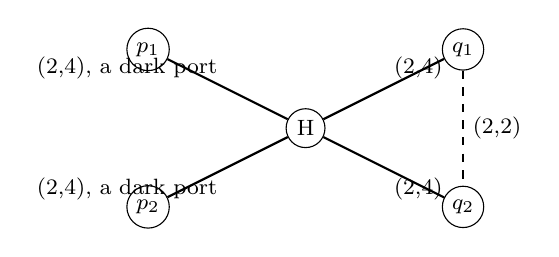
\begin{tikzpicture}[every node/.style={font=\footnotesize}]
\node[circle,draw,inner sep=2pt] (H) at (0,0) {H};
\node[circle,draw,inner sep=2pt] (p1) at (-2,1) {$p_1$};
\node[circle,draw,inner sep=2pt] (p2) at (-2,-1) {$p_2$};
\node[circle,draw,inner sep=2pt] (q1) at (2,1) {$q_1$};
\node[circle,draw,inner sep=2pt] (q2) at (2,-1) {$q_2$};
\draw[thick] (H) -- node[above left] {(2,4), a dark port} (p1);
\draw[thick] (H) -- node[below left] {(2,4), a dark port} (p2);
\draw[thick] (H) -- node[above right] {(2,4)} (q1);
\draw[thick] (H) -- node[below right] {(2,4)} (q2);
\draw[dashed] (q1) -- node[right] {(2,2)} (q2);
\end{tikzpicture}
\caption{The first depth web of the cross core. A hub H of dimension four with four (2,4) legs to qubits and one (2,2) pair, five sites and five links. The two pendant legs $p_1$ and $p_2$ at degree one are its dark ports, two of the six of the cross core.}
\end{figure}
\section{The count metric as the logarithm of the tower metric}\label{mod:X-5-D542610-lgtw-t1}
\begin{chconditional}[The count metric as the logarithm of the tower metric]\label{box:X-5-D542610-lgtw-t1:1}
Conditional on the entries this result rests on, each at its own standing. The count metric of the depth-metric open result is the logarithm of its tower metric: at every chain state of that open result the count metric, the cap 96 multiplied by the depth, equals the cap multiplied by the logarithm, to the rung base 36, of the tower metric over its origin 24, the logarithm exact at every chain state and equal to the depth, the tower the origin multiplied by the rung base to the depth, $24\cdot 36$ at every hub-unit pair at k 0, $31\,104$, $1\,119\,744$ and $40\,310\,784$ at k 1, 2 and 3 and 24 at the dock chains at k 0 where the depth is zero, equal at 28 of 28 chain states; the origin 24 equals the product of the three register dimensions 2, 3 and 4 at the dock web; the first parting of the depth-metric open result, the electron at k 0 with the tower $24\cdot 36$ against the count metric 96, is re-read equal as the origin offset, 96 multiplied by the logarithm 1 equal to 96 and at the depth zero 0 equal to 0; the unit reading beside, the base 6 and the origin 4, is exact and parts at every chain state, printed beside.
\end{chconditional}
\chstanding{conditional theorem}
\chdeps{Definitions 1.1 to 1.6 and Theorems 113.1 and 113.2}{no theorem beyond it at this release}
The tower metric and the count metric are read from the chain states of the depth-metric open result, the logarithm of the tower over its origin to the rung base is printed as an exact element at every state and compared with the count, and the origin is set beside the product of the register dimensions at the dock. The two metrics of that open result are one metric in two readings, the tower geometric and the count arithmetic, the logarithm carrying the one into the other with the origin as the offset. The register tower stands at its own chapter.
\begin{chbridge}
In statistical mechanics the entropy of a system is the logarithm of its number of states, so that a count that grows exponentially along a chain and a count that grows linearly are one quantity in two readings, and in a geometry a distance is additive while a volume multiplies \cite{Gibbs1902,Wald1984}. The correspondence is by name.
\end{chbridge}
\begin{chproof}[finite computation with its exact part]
\textit{The premises.} The axiom and the six definitions of Section~\ref{mod:FRAMEWORK}, definitions. The register tower and the metric of Section~\ref{mod:X-5-register-tower-and-the-metric}, a theorem. The depth metric and the serial link of the chapter titled The (2,2) genre, the pair ket, the serial link and the increment (chapter~\ref{mod:X-0-D540399-the-two-two-census-at-every-placement}, among the instruments), at their standings. The chain from the axiom to this result is four chapters deep.

\textit{The procedure.} The tower metric is read from the settled copies of the depth-metric open result at its ten chains and k 0 to 3, the seven chains and the three beside, at the depth readings and the tower readings, 480 cells; the rung base 36 and the origin 24 are read by locator from its rung cells, equal to the whole and the cut of the (2,3) read genre, the cut of the read genre multiplied by its whole re-met at the depth-scale entry at 48 of 48 and at the cut-register entry at 40 of 40. The logarithm of the tower over its origin to the rung base is taken as the greatest integer whose power of the base is at most the ratio, the remainder the ratio over that power, exact where the remainder is one. The count metric, the cap 96 multiplied by the depth, is compared with the cap multiplied by the exponent as an exact difference at every chain state, the first parting taken in the order of the chains and k. The origin is compared with the product of the distinct site dimensions of the dock web.

\textit{The totals.} At every chain state the tower reads the origin multiplied by the rung base to the depth, 24 at the depth 0 of the proton and the photon word at k 0, $24\cdot 36$ at the depth 1 of every hub-unit pair at k 0, and $31\,104$, $1\,119\,744$ and $40\,310\,784$ at the depths 2, 3 and 4, so the logarithm
\begin{equation}
\log_{36}\frac{24\cdot 36^{d}}{24} = d
\end{equation}
is exact at 600 of 600 cells over every reading, each tower reading geometric in its own base, and equal to the depth at 40 of 40 at the readings adopted, 0 at the dock chains, 1 at the hub-unit pairs and 2, 3, 4 at k 1, 2, 3, with 85 to 88 at the whole-web reading of the universe web. From the logarithm, by the cap, we obtain $96 d$ against the count metric $96 d$, the difference zero at every state, 0 against 0 at the depth 0, 96 against 96 at the depth 1 and 192, 288 and 384 against 192, 288 and 384 beyond, equal at 28 of 28 chain states and at every depth and tower reading at its own base, the whole-web reading 8160 against 8160 at k 0; the smallest instance is the electron at k 0, the tower $24\cdot 36$ over the origin 24 the base to the one, 96 multiplied by 1 equal to 96, which re-reads the first parting of the depth-metric open result as the origin offset. From the dock web of the electron, by its three distinct site dimensions, we obtain the origin
\begin{equation}
2\cdot 3\cdot 4 = 24,
\end{equation}
equal to the cut of the electron dock pair of the mass-unit entry with the rung base equal to its whole. The unit reading beside, four multiplied by 6 to the twice the depth plus one, is exact with the exponent twice the depth plus one and parts at every chain state, the electron at k 0 reading 96 against 288. So the rule pinned ahead reads face A yes and face B no with the first parting none.

\textit{The check.} The shifted origin moves the exponent at the electron from 1 to 0 and the deciding cell to no, the different base moves the logarithm inexact at every depth beyond zero, the (2,3) insertion in place of the (2,2) moves the depth at k 1 from 2 to 0 with the comparison standing, the text struck excludes the run, and the chain with no insertion moves every k to its k 0 state, 5 of 5 as pinned. The controls read the same at 16 of 16, among them the tower cells of the depth-metric open result at 480 of 480, its count metric at 80 of 80, the depth-scale entry at 48 of 48 and the distinct ratios 9, 162, 3888 and $104\,976$ re-derived. The result was reproduced by an independent route, two engines of different construction agreeing at every cell at both runs.
\chcert{600}
\end{chproof}
\begin{figure}[htbp]\centering
\scriptsize
\setlength{\tabcolsep}{3pt}
\begin{adjustbox}{max width=\linewidth}\begin{tabular}{llrrrrrr}
state & run & depth & tower & logarithm & cap by logarithm & count metric & difference \\ \hline
k0 & a1-a2 & 1 & eight hundred and sixty-four & 1 & 96 & 96 & 0 \\
k1 & a1-x1-a2 & 2 & 31104 & 2 & 192 & 192 & 0 \\
k2 & a1-x1-x2-a2 & 3 & 1119744 & 3 & 288 & 288 & 0 \\
k3 & a1-x1-x2-x3-a2 & 4 & 40310784 & 4 & 384 & 384 & 0 \\
\end{tabular}\end{adjustbox}
\caption{The count metric against the tower metric at the chain states of the electron web: the count metric is the cap 96 multiplied by the depth, the tower is the origin 24 multiplied by the rung base 36 to the depth, the logarithm of the tower over its origin to the rung base is the depth, and the difference between the count metric and the cap multiplied by the logarithm is zero at every state.}\label{fig:X-5-D542610-count-against-tower}
\end{figure}
\begin{figure}[h]
\centering
\begin{adjustbox}{max width=\linewidth}\begin{tabular}{rrr}
\hline
depth & $96 d$ from the logarithm & the count metric \\
\hline
0 & 0 & 0 \\
1 & 96 & 96 \\
2 & 192 & 192 \\
\hline
\end{tabular}\end{adjustbox}
\caption{The smallest instance, the electron at k 0: the tower $24\cdot 36$ over the origin 24 is the base to the one, so 96 multiplied by 1 equals 96, the origin offset of the depth-metric open result re-read; the difference zero at every depth.}
\end{figure}
\par\medskip\noindent{\itshape The next chapter reads the term the literature attaches to the vacuum.}\label{narr:close:10-5}\par
\section{The cosmological term at the depth exponent}\label{mod:X-6-cosmological-term-at-the-depth-exponent}
\chdesig{6-6}{10-6}{X-6-cosmological-term-at-the-depth-exponent}{X-6-D542582-w-tktu}
\label{narr:open:10-6}Theorem~115.1 reads the cosmological term at the depth exponent, resting on the link and the saturation.
\begin{chconditional}[The cosmological term at the depth exponent]\label{box:X-6-cosmological-term-at-the-depth-exponent:1}
Conditional on depth scale at the register tower, horizon at every rung from iterated closure and horizon register face at the closure, each at its own standing. The closure constant of the horizon register is thirty-six at every rung, the two faces of the register are related by the closure count alone, the ratio of the ladder objects at the two faces an exact power of the whole register, and one face names the term, the valence face at the closure count sixty-three equal to its free-direction bound, where the closure is saturated while the cap face is strict; so the cosmological term is an exact object at the valence face, the closure constant to the minus the depth exponent, the exact inverse of the ladder object at ninety-nine digits.
\end{chconditional}
\chstanding{conditional theorem}
\chdeps{Definitions 1.1 to 1.6, Theorems 9.1 to 9.7 and Open result 9.8 and Open results 245.1 and 245.2, Theorem 245.3, Open results 245.4 to 245.8 and Theorem 245.9}{the theorems of Chapters 1-2, 1-5, 4-1, 4-3, 5-3, 6-2, 6-6}
The closure constant of the horizon register is read at every rung of the register tower, the closure count re-derived from the universe web at the valence face and at the cap face and compared with the free-direction bound at each, the ladder objects formed at both faces and their ratio computed by exact division, and the term formed as the closure constant to the minus the depth exponent at the one face at which the closure is saturated. The cosmological term is the closure constant to the minus the depth exponent, an exact object at one reading of the horizon register, sixty-three at the valence reading and four hundred thirty-two at the cap reading, the one reading named the valence reading. What stands open is not a question of this chapter. The depth exponent at the valence face is a reading carried at a face the derivations do not fix, so the term as an exact object stands at that reading and its magnitude is not compared with observation here.
\begin{chbridge}
One term of this chapter stands beyond the framework, defined at its first use, \rosetta{the register tower}{a tower of Hilbert spaces of growing dimension}. The correspondence is by name, and no value of the term is displayed here.
\end{chbridge}
\begin{chproof}[finite computation with its exact part]
\textit{The premises.} The axiom and the six definitions of Section~\ref{mod:FRAMEWORK}, definitions. The link and its genres of Section~\ref{mod:I-2-link-and-its-six-genres}, definitions. The rungs and the horizon web of Section~\ref{mod:I-5-saturation-in-one-figure-seeds-waves-termination-sinks}, a theorem. The depth scale at the register tower of Section~\ref{mod:X-5-register-tower-and-the-metric}, a theorem under its posed count face. The horizon at every rung of Section~\ref{mod:X-3-horizon-at-every-rung-and-the-horizon-web-as-a-seeded-saturation} and the horizon register face at the closure, theorems. The join from shared, an open result consumed as a material. The chain from the axiom to this result is five chapters deep.

\textit{The exact part: the closure constant and the term.} The registers from the dimensions of the read genre (2,3) are the whole $36=4\cdot 9$ and the cut $24=8\cdot 3$. The register tower, listed at the figure, is the cut multiplied by the whole to the rung,
\begin{equation} \adjustbox{max width=\dimexpr\linewidth-3em\relax}{$\displaystyle T_k=24\cdot 36^{k}:\quad 24,\ 24\cdot 36,\ 31\,104,\ 1\,119\,744,\ 40\,310\,784,\ 1\,451\,188\,224,\ 52\,242\,776\,064\quad (k=0,\dots,6),$} \end{equation}
and from consecutive rungs, by exact division, we obtain the closure constant $T_k/T_{k-1}=36$ at every rung one to six, the law a power at the whole register. At the fixed interface the count is nine at every rung and the constant one. The closure count at each face is the readable spare of the universe web, $63$ at the valence face (over 60 sites) and $432$ at the cap face (over 369 sites). From the closure constant and the closure count, by the power, we obtain the ladder object $36^{63}$ at the valence face (an exact integer of ninety-nine digits) and $36^{432}$ at the cap face, their ratio $36^{369}$ an exact power of the whole register by exact division, so the two faces are related by the closure count alone. At the valence face the closure count $63$ equals its free-direction bound $63$, the closure saturated, while at the cap face $432$ stands against the bound $507$, strict. So the one face naming the term is the valence face, and the term is
\begin{equation}
\Lambda=36^{-63},
\end{equation}
the exact inverse of the ladder object, compared with nothing here. The smallest instance is the first rung, $(24\cdot 36)/24=36$, checked by hand.

\textit{The finite computation.} The input objects are the universe web (444 sites, 551 links, the one open dock on its tether to the closure site) and the eleven sequence rows of the horizon table. The enumeration rule computes the constant at every rung of every sequence as an exact rational. At the register face under the Weyl alphabet with the own-genre sub-clause the constants are $36$ at every rung, without the sub-clause $24$ at every rung, under the monomial alphabet the rational constants $31\,068/23$, $1\,119\,708/863$ and so on, parting at the second rung, and at the moving interface $1, 1/9, 9, 1/9, 9, 1/9$. The readings are eleven, with the law a power at five and parting at six. The cosmological term at the count-face exponent six beside is $36^{-6}$, equal to the scale cell of the depth-scale result. At the fixed interface the term is one, a trivial reading. The monomial and moving-interface readings leave the term undefined at the depth exponent.

\textit{The check.} Taking the cut as the constant, the interface count nine as the constant and the count-face exponent each move the term they name. Striking the text moves every cell. The result was reproduced by an independent route, two engines of different construction agreeing at every cell at both runs, with the registers of the horizon register face, the objects of the depth-scale result and the consumed files at 18 of 18 hashes as the controls.
\chcert{92}
\end{chproof}
\begin{figure}[h]
\centering
\begin{adjustbox}{max width=\linewidth}\begin{tabular}{llll}
\hline
rung & the register of the tower & the fixed interface & the closure constant \\
\hline
0 & 24 & 9 & \\
1 & $24\cdot 36$ & 9 & 36 \\
2 & 31\,104 & 9 & 36 \\
3 & 1\,119\,744 & 9 & 36 \\
4 & 40\,310\,784 & 9 & 36 \\
5 & 1\,451\,188\,224 & 9 & 36 \\
6 & 52\,242\,776\,064 & 9 & 36 \\
\hline
\end{tabular}\end{adjustbox}
\caption{The register tower of the horizon register at the rungs zero to six, the cut twenty-four multiplied by the whole thirty-six to the rung, with the count at the fixed interface nine at every rung and the closure constant thirty-six at every step.}
\end{figure}
\section{The serial (2,2) insertion at the metric}\label{mod:X-6-D540763-w-sttw}
\begin{chwall}[The serial (2,2) insertion at the metric]\label{box:X-6-D540763-w-sttw:1}
Face A, the per-link increment of the serial (2,2) insertion a constant of the placement, with the office increment zero at every chain and step, the metric increment equal to its first value and the cut increment zero, reads no. Face B reads yes with the first parting named. The metric stretches by one cell 96 per inserted link at every chain and body, 21 of 21 steps, and the register at the cut stays unmoved, 21 of 21, but the office by the body-alone rule moves at every uncapped body and every word, the electron by $536\,569/972 + (25/1458)\sqrt{2}$ at the first link, the muon by $847\,609/12 + (25/18)\sqrt{2}$, the tau by $3\,475\,947/4 + (25/2)\sqrt{2}$, the photon word by $202\,201/972 + (25/1458)\sqrt{2}$ and the body of the universe web by $917\,593/12 + (25/18)\sqrt{2}$, each growing at every further link, while the proton and the neutron read their inserted links beyond the entry at zero, the increment parting by body and by step; the first parting is the electron at the step 0 to 1, the office increment against zero.
\end{chwall}
\chstanding{open result}
\chdeps{Definitions 1.1 to 1.6, Theorems 99.1 and 99.2, Open results 99.3 and 99.4, Theorem 99.5 and Open result 99.6, Theorems 113.1 and 113.2, Theorem 115.1 and Theorem 195.1}{no theorem beyond it at this release}
Serial (2,2) links are inserted one by one into a chain of every body and of the universe web and three readouts are taken at every step, the office by the body-alone rule, the metric at its terminating wave and the register at the cut, so that the per-link increment of each is compared across chains and steps. The metric and the cut read one constant and the office does not, so the increment is no constant of the placement. The register tower and the body-alone rule stand at their own chapters.
\begin{chbridge}
In the literature a photon added to a bound state changes its energy by a self-energy that depends on the state, while the length of a path grows by one unit per quantum of length regardless of what the path passes through \cite{Weinberg1995,Wald1984}. The correspondence is by name.
\end{chbridge}
\begin{chproof}[finite computation]
\textit{The premises.} The axiom and the six definitions of Section~\ref{mod:FRAMEWORK}, definitions. The register tower and the metric of Section~\ref{mod:X-5-register-tower-and-the-metric}, a theorem. The body-alone office rule of Section~\ref{mod:VIII-2-body-alone-office-rule}, a theorem. The horizon web at its cap of Section~\ref{mod:X-3-horizon-at-every-rung-and-the-horizon-web-as-a-seeded-saturation}, an open result. The chain from the axiom to this result is five chapters deep.

\textit{The procedure.} The input objects are nine webs with a chain each, the electron web at its hub-unit pair, 9 sites and 10 links at k zero, the muon at 13 and 15, the tau at 17 and 20, the proton at its dock chain, 8 and 9, a web with no (2,2) link, the neutron through the deuteron, 26 and 28, the photon word at the bulk of its alternating chain, 6 and 5, the universe web within its body B00, 444 sites and 551 links, and beside them the neutron of the seeds and the tau sink, 13 and 16 and 16 and 19. At every step k from 0 to 3 one site of dimension 2 is inserted in series at the chain link, the site and link counts and the (2,2) count growing by one and every other genre unchanged, the rule a hub-unit pair at 7 of 9 chains and the first unentered dock chain at the proton and the photon word. Three readouts are taken at every chain and k: the office by the body-alone rule at the typed segment reading, the metric at the shared reading at its terminating wave with every link at its cap, and the register at the cut.

\textit{The totals.} The first powers at the inserted links read 67, 71, 75, 79 at the electron with the act 4, 963, 999, 1035, 1071 at the muon with the act 36, 3969, 4077, 4185, 4293 at the tau with the act 108, 2871 unmoved at the proton and the neutron with the act 0, 24, 28, 32, 36 at the photon word with the act 4 and 1044, 1080, 1116, 1152 at the body of the universe web with the act 36, the k zero cells equal to the settled offices at 6 of 6 reads. The office increment per inserted link is the difference of the squares of the first powers plus the closure increment at the dressing, so at the electron at the first step
\begin{equation}
71^2 - 67^2 + \frac{25}{972} + \frac{25}{1458}\sqrt{2} = 552 + \frac{25}{972} + \frac{25}{1458}\sqrt{2} = \frac{536\,569}{972} + \frac{25}{1458}\sqrt{2},
\end{equation}
the smallest instance, and at the muon at the dressing 9
\begin{equation}
999^2 - 963^2 + \frac{25}{12} + \frac{25}{18}\sqrt{2} = 70632 + \frac{25}{12} + \frac{25}{18}\sqrt{2} = \frac{847\,609}{12} + \frac{25}{18}\sqrt{2},
\end{equation}
the identity of the pair part with the first power squared holding at 36 of 36 cells. The metric reads $513\,055$ at the universe web at k zero, the register at wave 0 $501\,661$ plus the growth $11\,394$, then $513\,151$, $513\,247$ and $513\,343$, every inserted link at its cap 96 from wave 0; the electron 8613, 8709, 8805, 8901; the proton 10224 to 10512; the photon word 1595 to 1883; the increment one cell 96 at 21 of 21 steps. The register at the cut reads 6561 at the whole face, 4096 at the cut face and 81 at the rank face at every chain and every k, the inserted links within one body crossing no wire, the increment 0 at 21 of 21. The office increment reads the elements of the box at the first step of the five uncapped chains and 0 at the proton and the neutron, so the rule pinned ahead reads face A no and face B yes with the first parting the electron at the step 0 to 1.

\textit{The check.} The inserted links declared wires of the cut move the cut register, the metric read at the key rule at wave 0 moves the register of the universe web to $391\,711$, the dressing struck to one moves the first power of the muon to 107, the inserted sites read as qutrits move the metric increment to 542 and the text struck excludes the run, 5 of 5 as pinned. The controls read the same at 16 of 16, among them the settled offices at 6 of 6, the count law and the caps 96, 319, 906, 1036, 2053 and 5100 at the six genres, and the copied body-alone engines re-run at 24 of 24 cells. The result was reproduced by an independent route, two engines of different construction agreeing at every cell at both runs.
\chcert{36}
\end{chproof}
\section{The serial (2,2) link at the washed Laplacian}\label{mod:X-6-D541010-w-stwl}
\begin{chwall}[The serial (2,2) link at the washed Laplacian]\label{box:X-6-D541010-w-stwl:1}
Face A, the increment of the washed Laplacian of the universe web per serial (2,2) link a uniform term at every site of the chain, a constant added to the washed curvature, reads no at 21 of 21 cells of k and rung. Face B reads yes with the parting named. At the chain of the body S from B09.f1 to B09.f2 and at every k 1 to 3 and every rung 0 to 6 the increment is the local one-link difference of the subdivision, two one-link Laplacians added at the new site and one removed at the subdivided link, supported at three sites with the trace 2, the row sums zero, the rank 2 and the spectrum $-1$, 0 and 3 on its support, equal to the one-link Laplacian of the (2,3) rung at the trace and the row sums and parting from it at the spectrum and the rank; restricted to the chain sites its diagonal reads 0 at the old sites and 2 at the new site with the off-diagonal cells $-1$ and 1, the first parting at the first chain site B09.f1 at the cell to B09.i1, 0 against $-1$, and the row sums zero at every site admit the zero term alone as a uniform term, so that no constant is added to the washed curvature at the sites by a serial (2,2) link.
\end{chwall}
\chstanding{open result}
\chdeps{Definitions 1.1 to 1.6, Theorems 90.1 to 90.4 and Theorem 115.1}{no theorem beyond it at this release}
The chain of the body S is subdivided in series one site at a step, the washed Laplacian of every inserted web is recomputed at every rung of the ladder, and the increment per inserted link is compared with a uniform term at the chain sites and with the one-link Laplacian of the rung. The increment is a local difference at three sites and no term at the sites. The curvature as the washed Laplacian stands at its own chapter.
\begin{chbridge}
On a lattice the discrete Laplacian of a graph is the sum over its links of one-link Laplacians, and refining the lattice by one site changes the operator locally while a cosmological constant adds the same term at every site \cite{Chung1997,Einstein1917}. The correspondence is by name.
\end{chbridge}
\begin{chproof}[exhaustive census with its exact part]
\textit{The premises.} The axiom and the six definitions of Section~\ref{mod:FRAMEWORK}, definitions. The curvature as the graph Laplacian washed over the ladder of Section~\ref{mod:X-1-curvature-as-the-graph-laplacian-washed-over-the-ladder}, a theorem. The chain from the axiom to this result is three chapters deep.

\textit{The census.} The set counted is the (2,2) chains of the universe web, 444 sites, 551 links and 27 components with the open dock: 85 chains, every one a pair of qubit legs of one hub joined by one (2,2) link, the chain adopted the first bulk chain in link order, the chain 16 from B09.f1 to B09.f2 in the body S. The inserted webs at k 0 to 3 carry 444 to 447 sites, 551 to 554 links and 85 to 88 (2,2) links with 27 components at every k, the chain run growing by one site of dimension 2 at a step. The washed Laplacian of every inserted web at the rungs 0 to 6 carries the trace 1102, 1104, 1106 and 1108 at rung 0, two per inserted link, the row sums zero at every site and the kernel 27 equal to the components at every web and rung, the copied engines of the curvature chapter run unedited at the inserted webs re-meet their settled captures at k 0 and the 1288 Laplacian, wash and tensor cells at 1288 of 1288 at every k and rung. The increment per inserted link, the difference of the Laplacians with the older one extended by zero, is supported at the three sites of the step, at k 1 the sites B09.f1, B09.i1 and B09.f2, with the cells of the figure, the trace 2, the row sums zero, the rank 2, the polynomial $x^3 - 2x^2 - 3x$ and the spectrum $-1$, 0, 3, the decomposition two one-link Laplacians added and one removed, equal at every rung and at the ladder wash at 21 of 21 cells; the one-link Laplacian of the (2,3) rung of the connection table at its 18 steps has the trace 2, the row sums zero, the rank 1 and the spectrum 0, 2, equal at the trace and the row sums and parting at the spectrum and the rank. The smallest case is the chain at k 1, worked at the figure: the uniform term the row sums admit is the zero term and the diagonal reads 0, 2, 0. The result is certified at the repository.

\textit{The check.} The uniform strike moves the face to yes with the row sums off zero, the extension struck moves the trace to 0, the chain rule struck moves the chain to a rung component, the genre struck moves the inserted sites to dimension 3, the serial strike as a parallel pendant moves the increment to the one-link Laplacian itself, and the text struck excludes the run, 6 of 6 as pinned. The controls read the same at 14 of 14. The result was reproduced by an independent route, two engines of different construction agreeing at every cell at both runs.
\chcert{1288}
\end{chproof}
\begin{figure}[h]
\centering
\begin{adjustbox}{max width=\linewidth}\begin{tabular}{lrrr}
\hline
site & B09.f1 & B09.i1 & B09.f2 \\
\hline
B09.f1 & 0 & $-1$ & 1 \\
B09.i1 & $-1$ & 2 & $-1$ \\
B09.f2 & 1 & $-1$ & 0 \\
\hline
\end{tabular}\end{adjustbox}
\caption{The smallest case, the chain at k 1: the increment of the washed Laplacian per inserted link at its three sites, the trace 2, the row sums zero, the rank 2 and the spectrum $-1$, 0, 3; the diagonal 0, 2, 0 admits the zero uniform term alone.}
\end{figure}
\section{The reservoir cell and the pair ket}\label{mod:X-6-D541128-rcpm-t1}
\begin{chtheorem}[The reservoir cell and the pair ket]\label{box:X-6-D541128-rcpm-t1:1}
The reservoir cell (2,2) of the horizon term and the pair ket at the join are one object under the body-alone rule, the horizon reading and the bulk reading of one genre: the reservoir cell is located at 5 of 5 parents and the pair ket at its entry at 23 of 23 cells, the ten shared cells are equal, the genre (2,2), the sites 2 and 2, the registers 16 and 9, the Born cell 96, the one-exchange 30, the office 0 at the pendant placement and $15577/972 + (25/1458)\sqrt{2}$ at the interior placement, the order 1 and the two electromagnetic kinds, and every (2,2) link of the horizon web stands at the office of the bulk object at its placement, 7 pendant and 78 interior of 85, and every one of the web table at 255 of 255, 10 pendant and 245 interior, so the horizon is a placement of the bulk object; the first parting is none.
\end{chtheorem}
\chstanding{theorem}
\chdeps{Definitions 1.1 to 1.6, Theorems 9.1 to 9.7 and Open result 9.8, Theorems 99.1 and 99.2, Open results 99.3 and 99.4, Theorem 99.5 and Open result 99.6, Theorem 115.1 and Theorem 195.1}{no theorem beyond it at this release}
The one (2,2) token of the horizon term, the free-pair count of its first law at one quantum, is traced to its parents, the cut-register formula at the dimensions 2 and 2, the horizon web with its 85 (2,2) links at the cap 96, the universe web and the genre table, and the pair ket at the join is read at its entry; the cells the two share are compared one by one and the office is read at every (2,2) link of the horizon web at its placement. The cosmological fence is doubled here: no constant and no density enters any cell. The pair ket and the body-alone rule stand at their own chapters.
\begin{chbridge}
In the literature the vacuum energy that gravitates at a horizon and the photon exchanged between two charges are objects of two theories, a cosmological reservoir and a gauge quantum, with no identity between them \cite{Weinberg1987,Peskin1995}. The correspondence is by name.
\end{chbridge}
\begin{chproof}[finite computation]
\textit{The premises.} The axiom and the six definitions of Section~\ref{mod:FRAMEWORK}, definitions. The link and its six genres of Section~\ref{mod:I-2-link-and-its-six-genres}, definitions. The body-alone office rule of Section~\ref{mod:VIII-2-body-alone-office-rule}, a theorem. The horizon web as a seeded saturation of Section~\ref{mod:X-3-horizon-at-every-rung-and-the-horizon-web-as-a-seeded-saturation}, a theorem, and the cosmological term of Section~\ref{mod:X-6-cosmological-term-at-the-depth-exponent}, a theorem. The chain from the axiom to this result is five chapters deep.

\textit{The procedure.} The reservoir cell is located at its five parents: the one (2,2) token of the horizon term at its first-law line, the free-pair count at one quantum; the cut-register formula instantiated at the dimensions 2 and 2; the horizon web with 85 (2,2) links at the seed and the cap 96; the universe web parsed whole at 444 sites and 551 links with 85 (2,2) links; the genre table at the pair 2 and 2 at the order 1 with the carriers of the electromagnetic and the weak. The pair ket at the join is located at its entry at 23 cells, the genre, the sites, the registers, the 57 records of the two reads at the sectors 24, 18, 12 and 3, the second-order cell, the Born cell, the one-exchange and the two-exchange, the offices at both placements, the order and the kinds. The ten cells the two objects share are then compared one by one, and the office is read at every (2,2) link of the horizon web at its placement under the rule, a link at a qubit end of degree one in the dock set struck at the office 0 and a link at two shared ends unstruck.

\textit{The totals.} From the dimensions 2 and 2, by the register formula, we obtain the whole $(2\cdot 2)^2 = 16$ and the cut $(2^2-1)(2^2-1) = 9$. From the four sectors of the records at the gains 1, 2, 2 and 4, by the count law, we obtain the Born cell
\begin{equation}
96 = 24 + 18\cdot 2 + 12\cdot 2 + 3\cdot 4,
\end{equation}
the cap of the (2,2) genre at the horizon web, the smallest instance worked on the page. From the act 4 at an unstruck link, by the body-alone rule, we obtain the interior office $4^2 + 25/972 + (25/1458)\sqrt{2} = 15577/972 + (25/1458)\sqrt{2}$ and at a pendant link the office 0. The ten shared cells, the genre, the sites, the two registers, the Born cell, the one-exchange 30, the two offices, the order and the two electromagnetic kinds, are equal at 10 of 10 between the horizon reading and the bulk reading. At the horizon web the 85 (2,2) links stand 7 pendant at the office 0 and 78 interior at the unstruck office, the hub dressing 1 at every one with both ends qubits, and at the web table the 255 (2,2) links stand 10 pendant and 245 interior, the reads beside at 2 of 2; the first parting is none, so the rule pinned ahead reads face A yes and face B no.

\textit{The check.} The horizon Born cell swapped for the (2,3) entry 319 moves the Born identity, the horizon links all struck moves the interior office, the horizon genre struck to (3,3) moves the one-exchange to 200 and the registers to 81 and 64, the bulk object replaced by the web table word moves the office at the pendant placement to 576, and the text struck excludes the run, 5 of 5 as pinned. The controls read the same at 16 of 16, among them the caps by genre 96, 319, 906, 1036, 2053 and 5100 equal to the Born counts at 6 of 6 and the genres of the horizon web, 85, 34, 229, 134, 67 and 2, equal to the seed cells. The result was reproduced by an independent route, two engines of different construction agreeing at every cell at both runs.
\chcert{255}
\end{chproof}
\section{The tick as the office of one serial (2,2) link}\label{mod:X-6-D542582-w-tktu}
\begin{chwall}[The tick as the office of one serial (2,2) link]\label{box:X-6-D542582-w-tktu:1}
Face A, the office of one serial (2,2) link one element at every chain, so that the tick is the (2,2) cell as its own unit, reads no. Face B reads yes with the first parting named: the office of one serial (2,2) link, the increment of the serial entry read as an office, parts by chain at the first comparison, the muon against the electron, $847\,609/12 + (25/18)\sqrt{2}$ against $536\,569/972 + (25/1458)\sqrt{2}$, 6 distinct cells at the seven chains with zero at the two capped bodies, equal to the tick 1 at none and to a cell of the register tower at none, the tower re-met at 7 of 7 rungs and the office carrying a root-two part at every uncapped chain; the one rule of the tick-scale open result re-posed with that office as the tick re-meets the settled ratios at the electron alone, 1 of 4; at the link-alone reading per dressing squared beside, the five uncapped chains read one element, $15577/972 + (25/1458)\sqrt{2}$, the (2,2) act squared 16 plus the (2,2) closure increment, and the capped bodies read zero, printed beside.
\end{chwall}
\chstanding{open result}
\chdeps{Definitions 1.1 to 1.6, Theorems 113.1 and 113.2, Theorem 115.1, Open result 122.1 and Theorem 195.1}{no theorem beyond it at this release}
The tick is transcribed from the one-link and depth-step theorems and the tick-scale open result, the office of one serial (2,2) link is read at every chain of the serial entry as its increment, and the open result is re-posed with that office as the tick against the tick 1, the (2,2) registers and the register tower. The office parts by chain, so the tick-scale open result is re-posed and not met. The tick scale and the register tower stand at their own chapters.
\begin{chbridge}
In the literature a clock ticks in one unit and a quantum of a field carries one unit of energy at a given frequency, so that the energy of one photon would be the same quantum of the clock wherever it is emitted \cite{Planck1899,Wilczek2005}. The correspondence is by name.
\end{chbridge}
\begin{chproof}[finite computation with its exact part]
\textit{The premises.} The axiom and the six definitions of Section~\ref{mod:FRAMEWORK}, definitions. The tick scale as a coupling scale of Section~\ref{mod:X-10-tick-scale-as-a-coupling-scale}, an open result. The register tower of Section~\ref{mod:X-5-register-tower-and-the-metric}, a theorem. The body-alone office rule of Section~\ref{mod:VIII-2-body-alone-office-rule}, a theorem. The chain from the axiom to this result is five chapters deep.

\textit{The procedure.} The tick is transcribed: the one-link theorem at the reach 1 link per instance and 0 per read with the move-tick map zero at 9 of 9 moves over 32851 instances, the depth-step theorem at the increment zero at 8 of 8 moves and 32 of 32 move faces over 29703 instances, and the tick-scale open result at its one rule, a mass in the electron unit the office multiplied by the register ratio at the one tick, the tick 1 at 4 of 4 unit lines and the registers at the one tick 36 at the electron, the muon and the proton and 16 at the tau, the rule re-met at the mass at 4 of 4 and at the settled ratio at 3 of 4 with the tau the one that differs. The office of one serial (2,2) link at a chain is the office at k one less the office at k zero at the typed segment reading of the serial entry, read at its seven chains and the two beside. The open result is re-posed by comparing that office across the chains as one element, against the tick 1, against the (2,2) whole 16, cut 9 and cap 96, and against the cells of the register tower at the rungs 0 to 6.

\textit{The totals.} The office of one serial (2,2) link reads at the electron $536\,569/972 + (25/1458)\sqrt{2}$, the first power 67 to 71 at the act 4 with the cross term 536 and the closure increment $25/972 + (25/1458)\sqrt{2}$, at the muon $847\,609/12 + (25/18)\sqrt{2}$ at the act 36 and the dressing 9, at the tau $3\,475\,947/4 + (25/2)\sqrt{2}$ at the act 108 and the dressing 27, 0 at the proton and the neutron, at the photon word $202\,201/972 + (25/1458)\sqrt{2}$ at the first power 24 and the act 4, and at the body of the universe web $917\,593/12 + (25/18)\sqrt{2}$ at the first power 1044 and the act 36, equal to the increment cells of the serial entry at 9 of 9 chains and the office identity at 18 of 18 cells. The smallest instance is the electron,
\begin{equation}
71^2 - 67^2 + \frac{25}{972} + \frac{25}{1458}\sqrt{2} = \frac{536\,569}{972} + \frac{25}{1458}\sqrt{2},
\end{equation}
worked on the page. Across the seven chains the office takes 6 distinct cells, the first parting the muon against the electron; it equals the tick 1 at 0 of 7, the whole 16, the cut 9 and the cap 96 at 0 of 7 each, and a cell of the tower, 24 multiplied by 36 to the rung at 7 of 7 rungs re-met, at 0 of 7, the surd part nonzero at every uncapped chain and the valuation of the rational part at the prime 2 reading 2 at every uncapped chain. The one rule re-posed with the office as the tick, the tick ratio the office at the chain over the office at the electron, re-meets the settled ratio at the electron alone and parts first at the muon. So face A reads no at the one-element cell and face B reads yes with the first parting named; the readings beside, the increment per dressing squared at 6 distinct cells, the link-alone cell at 4 and the link-alone cell per dressing squared at 2 with the five uncapped chains at one element, are printed alongside the two faces.

\textit{The check.} The inserted link read at the (2,3) measure, two serial links in place of one, the increment struck to the cell of the first chain, which moves the one-element cell to yes, the tower read at a shifted rung and the text struck each move the cells they name, 5 of 5 as pinned. The controls read the same at 14 of 14, among them the serial entry re-met at its increments 9 of 9, the tick-scale open result at its registers 24 of 24 and the tower at 7 of 7 at three readings. The result was reproduced by an independent route, two engines of different construction agreeing at every cell at both runs.
\chcert{7}
\end{chproof}
\begin{figure}[h]
\centering
\begin{adjustbox}{max width=\linewidth}\begin{tabular}{lll}
\hline
chain & the working & the cell \\
\hline
the electron & $71^2 - 67^2 + 25/972 + (25/1458)\sqrt{2}$ & $536\,569/972 + (25/1458)\sqrt{2}$ \\
the photon word & the first power 24 at the act 4 & $202\,201/972 + (25/1458)\sqrt{2}$ \\
the body of the universe web & the first power 1044 at the act 36 & $917\,593/12 + (25/18)\sqrt{2}$ \\
\hline
\end{tabular}\end{adjustbox}
\caption{The smallest instance, the electron, with the photon word and the body of the universe web beside: the office cell at the chain, equal to the increment cells of the serial entry at 9 of 9 chains.}
\end{figure}
\par\medskip\noindent{\itshape The sinks without a dock are read in the next chapter.}\label{narr:close:10-6}\par
\section{Dark matter as the dock-free sinks}\label{mod:X-7-dark-matter-as-the-dock-free-sinks}
\chdesig{6-7}{10-7}{X-7-dark-matter-as-the-dock-free-sinks}{X-7-dark-matter-as-the-dock-free-sinks}
\label{narr:open:10-7}Open result~120.3 states dark matter as the dock-free sinks, with the structure counts at the dark cut, Open result~120.1, and the dark acting centers as the structure counts, Open result~120.2, every one an open result.
\begin{chwall}[Structure counts at the dark-cut]\label{box:X-7-dark-matter-as-the-dock-free-sinks:1}
At every dark (3,3) cut of the dark-cut admissibility question the triangle count changes by minus one, the star count is unchanged and the per-corner vector changes at every one, so the difference of the star count and the triangle count is conserved at none and is no second-order invariant, the lepton number alone changing at second order, under the one-act clause as the ancestors print it.
\end{chwall}
\chstanding{open result}
\chdeps{Definitions 1.1 to 1.6, Theorems 9.1 to 9.7 and Open result 9.8, Theorems 28.1 and 28.2, Open results 28.3 and 28.4 and Theorem 28.5, Open results 241.1 and 241.2, Theorems 241.3 and 241.4 and Open results 241.5 to 241.7 and Open results 245.1 and 245.2, Theorem 245.3, Open results 245.4 to 245.8 and Theorem 245.9}{Theorem 255.1}
\begin{chwall}[Dark acting centres as the structure counts]\label{box:X-7-dark-matter-as-the-dock-free-sinks:2}
The two dark acting centres, the (2,4) and (3,4) centres of the centre census, are conserved at every interaction as functionals of the typed count, but the matching of the centres to the junction count and the triangle count agrees at a minority of the webs at both assignments, so the two centres are two conserved charges with no Standard Model name, their carriers the webs carrying a (2,4) link and those carrying a (3,4) link, a prediction stated and not adopted.
\end{chwall}
\chstanding{open result}
\chdeps{Definitions 1.1 to 1.6, Theorems 9.1 to 9.7 and Open result 9.8, Theorems 28.1 and 28.2, Open results 28.3 and 28.4 and Theorem 28.5, Open results 241.1 and 241.2, Theorems 241.3 and 241.4 and Open results 241.5 to 241.7 and Open results 245.1 and 245.2, Theorem 245.3, Open results 245.4 to 245.8 and Theorem 245.9}{Theorem 255.1}
\begin{chwall}[Dark matter as the dock-free sinks]\label{box:X-7-dark-matter-as-the-dock-free-sinks:3}
The rule that a web is neutral exactly when it carries no (2,3) dock, checked against the derived charges over the webs censused at their dock count, parts at the docked webs of charge zero, the first parting web the docked S web; the released object and the dark candidates of the readability order, the kind readable by no photon, lie in the dock-free kind at both readings. Face A, the dock-free kind and the charge-zero kind one kind at the typed webs, reads no. Of the 140 webs whose charge is typed, every one reads charge zero at the first spelling, while the dock-free webs among them are fewer. Face B reads yes, and the parting is named. No dock-free web stands at a nonzero charge, but fifty-two docked webs stand at charge zero, the first the docked S web of ten sites and eleven links with one (2,3) dock.
\end{chwall}
\chstanding{open result}
\chdeps{Definitions 1.1 to 1.6, Theorems 9.1 to 9.7 and Open result 9.8, Theorems 28.1 and 28.2, Open results 28.3 and 28.4 and Theorem 28.5, Open results 241.1 and 241.2, Theorems 241.3 and 241.4 and Open results 241.5 to 241.7 and Open results 245.1 and 245.2, Theorem 245.3, Open results 245.4 to 245.8 and Theorem 245.9}{Theorem 255.1}
This chapter carries three open questions and no theorem. The first evaluates the star count, the triangle count and the per-corner vector at every dark cut and finds the difference conserved at none. The second enumerates the dark acting centres as functionals of the typed count, checks their conservation at every interaction and matches them against the structure counts at both assignments, the matching parting at both. The third censuses the docks of every web and checks the neutrality rule against the derived charges, the two kinds parting at the docked webs of charge zero. The dark genre and its readability stand at the confinement chapter. What stands open is the identity of the dark sinks as the dock-free webs at the parting of the neutrality rule, the two dark acting centres as charges with no name, and the second-order invariant that the dark cut does not conserve. The dark fraction as a register ratio stands at its own open question.
\begin{chbridge}
Three terms of this chapter stand beyond the framework, each defined at its first use, \rosetta{the acting centre}{the center of an algebra of observables}, \rosetta{the released object}{a decay product} and \rosetta{the dart}{a directed edge of a graph}. The correspondence is by name.
\end{chbridge}
\begin{chproof}[exhaustive census]
\textit{The premises.} The axiom and the six definitions of Section~\ref{mod:FRAMEWORK}, definitions. The link and its genres of Section~\ref{mod:I-2-link-and-its-six-genres}, definitions. The moves of Section~\ref{mod:I-4-moves-in-one-table}, definitions. The sinks of Section~\ref{mod:I-5-saturation-in-one-figure-seeds-waves-termination-sinks}, a theorem. The read at a register of Section~\ref{mod:I-6-read-at-a-register-the-probe-and-the-measurement}, a theorem. The dart as the unit weight, the neutral sinks census, the photon join face and the readability order, theorems. The released object, the library webs as seeds, the bound-respecting seed and the kernel results, open results consumed at their tables. The chain from the axiom to this result is five chapters deep.

\textit{The census.} The set counted is the webs, 2551 in all, generated from five families (the library 64, the seeded sinks of the library webs 2203, the neutral sinks 247, the released object 21, the bound-respecting seed 16), every web spelled as sites and links. The property tested at each web is its (2,3) dock count at the reading adopted (a pendant qubit at a qutrit), with every (2,3) link counted at the reading beside, and its derived charge where a derived charge is typed, the dart as the unit weight. The counts by dock count at the reading adopted are
\begin{equation}
0{:}1309,\quad 1{:}548,\quad 2{:}539,\quad 3{:}61,\quad 4{:}44,\quad 5{:}41,\quad 6{:}9 ,
\end{equation}
the zero kind 1309 of 2551 (and 1036 at the reading beside), the derived dock columns re-met at 2506 of 2506. The derived charge is typed at 140 webs, every one at charge zero at the first spelling. The rule that a web is neutral exactly when it carries no (2,3) dock holds at 88 of 140 and parts at 52 of 140, the partings every one a docked web at charge zero and none a dock-free web at a nonzero charge. The first parting element is the docked S web (ten sites, eleven links, one (2,3) dock, the charge zero at the first spelling and nonzero at the shared and cut spellings), which is the parting the box names. The released object derived, the one anatomy at the measure 28, lies in the zero kind at both readings, and the dark candidates of the readability order, the 1036 webs readable by no photon, lie in the zero kind at 1036 of 1036 at both readings. The smallest case is the up quark web, three sites and two links with no (2,3) dock and the charge zero, checked by hand.

\textit{The check.} At every other spelling of the charge (the shared, cut and cut-shared spellings and the kernel functionals) the partings move (87, 90, 90 and 287 of their counts) and the first parting web moves with them. The dock count at the reading beside moves the partings to 67. Striking the text moves every cell. The result was reproduced by an independent route, two engines of different construction agreeing at every cell, the census strings of three spellings ordered differently by the two routes and counted apart as a presentation and no cell, the controls at 13 of 14 beside.
\chcert{2551}
\end{chproof}
\par\medskip\noindent{\itshape The horizon returns in the next chapter as a non-sink.}\label{narr:close:10-7}\par
\section{The uncapped genre as the depth}\label{mod:X-7a-D542798-w-ncgu}
\chdesig{6-7a}{10-7a}{X-7a-D542798-w-ncgu}{X-7a-D542798-w-ncgu}
\begin{chwall}[The uncapped genre as the depth]\label{box:X-7a-D542798-w-ncgu:1}
Face A, one uncapped genre named at the three closure partings and its chain the depth as one object, reads no. Face B, another genre than (2,2) named at the three, reads no. Neither face holds, with the first parting named: the three closure open results part at three different genres, the cap reachable by genre first at (2,4) with the letter open against the order expecting locked, the genre closure of the seeded saturations at a made end of dimension 3, a (2,3) link at the link reading, and the sector identity at (2,2) at every one of its 11 lines, and the termination census names two, (3,3) at the joins first in table order and (2,2) at the pair link of the hub unit at the site-creating reading, so no one uncapped genre is named; the (2,2) chain, the serial insertion with 2, 3 and 4 inserted links at k 1, 2 and 3 and the metric stretched by one cell 96 per link, is not equal to the depth as one object, the dark-port count 6 counting 3 ports at (2,2) and 3 at (2,4) and the depth of the unstopped saturation a lower bound 3 of waves at no genre; the register of the (2,2) genre at the cap census of the horizon web grows by 252 at the one rung to its terminating wave at the shared reading, 7 uncapped (2,2) links at 36 each, and by 0 beyond and at the key reading, printed and compared with nothing; the first parting is the cap reachable by genre at (2,4) against the genre closure at 3.
\end{chwall}
\chstanding{open result}
\chdeps{Definitions 1.1 to 1.6, Theorems 9.1 to 9.7 and Open result 9.8, Theorems 105.1 and 105.2, Open results 105.3 to 105.5 and Theorem 105.6 and Open results 245.1 and 245.2, Theorem 245.3, Open results 245.4 to 245.8 and Theorem 245.9}{no theorem beyond it at this release}
The three closure open results are transcribed at their parting cells from the copies, the genre named at each parting is compared pairwise and against the termination census at two readings, the (2,2) chain is set beside the dark-port count and the lower-bound depth, and the growth of the register per rung is printed at the two readings of the unstopped saturation and the four readings of open at the cap census. The reading that named the one genre at which the closure open results part and called it the (2,2) chain is not met at the settled cells. The depth and the universe web stand at their own chapters.
\begin{chbridge}
In a cosmology the dimension of space is the exponent of the growth of a ball with its radius \cite{Friedmann1922,Weinberg1995}. The correspondence is by name.
\end{chbridge}
\begin{chproof}[finite computation with its census]
\textit{The premises.} The axiom and the six definitions of Section~\ref{mod:FRAMEWORK}, definitions. The link and its six genres of Section~\ref{mod:I-2-link-and-its-six-genres}, definitions. The saturation with its seeds, waves and termination of Section~\ref{mod:I-5-saturation-in-one-figure-seeds-waves-termination-sinks}, a theorem. The depth as the growth order and the termination wave of Section~\ref{mod:X-4-depth-the-growth-order-and-the-termination-wave}, open results, and the depth of the universe web of the chapter titled The depth of the universe web (chapter~\ref{mod:X-7a-D542798-w-ncgu}), at its standing. The chain from the axiom to this result is five chapters deep.

\textit{The procedure.} The three closure open results are read at their parting cells from the settled copies: the cap reachable by genre at its six letters at the passage reading, the genre closure of the seeded saturations at its first made end outside the closure, and the sector identity at the first parting genre of each of its 11 lines. The genre at each parting is re-derived from the cell and the three are compared pairwise at an end reading and a link reading. The termination theorem is read at its face naming the first move that adds a site without bound at two readings, and the genre at which the site-creating growth re-applies is read at the web of its seed. The (2,2) chain of the serial entry is set beside the dark-port count of the depth-scale entry and the lower-bound depth of the unstopped saturation, and the register growth per rung is read at the shared, key, valence and key-and-shared readings of the cap census of the horizon web.

\textit{The totals.} The cap reachable by genre reads open at the five genres (2,2) to (3,4) and locked at (4,4) at the shared passage reading against the readability order open, open, locked, locked, locked, locked, the parting genres (2,4), (3,3) and (3,4) at 3 of 6 and the first (2,4); the genre closure parts at the web 19 of the pair-ket root seed at wave 2 by the reverse hub move, three sites of the dimensions 2, 2 and 3 with the links (2,2) and (2,3), the made qutrit linked to a qubit, the genre 3 at the end reading and (2,3) at the link reading; the sector identity parts at (2,2) at 11 of 11 lines. So the genres at the three partings are (2,4), 3 and (2,2) at the end reading and (2,4), (2,3) and (2,2) at the link reading, three distinct at both, and one genre at the three is none. The termination theorem terminates every seeded saturation under the site bound and with the bound lifted grows first at the (3,3) join in table order and at the (2,2) pair link of the hub unit at the site-creating reading, the seed web of five sites with the link census 1, 3, 1 at (2,2), (2,4) and (3,4) carrying the one pair link, so the census names two genres and one genre at the census is none. The (2,2) chain at the electron carries the inserted links 0, 2, 3, 4 at k 0 to 3, every one of the genre (2,2), with the metric increment 96 at 21 of 21 steps, while the dark-port count 6 counts the ports
\begin{equation}
3 \text{ at } (2,2) + 3 \text{ at } (2,4) = 6,
\end{equation}
the ports at the chain genre 3 of 6, and the depth of the unstopped saturation is a lower bound 3 at the wave reached 2, a count of waves at no genre, so the chain is equal to the depth as one object at no reading, the first parting the dark-port count 6 against the ports at (2,2) 3. The register growth of the (2,2) genre at the horizon web reads 252 at rung 1 and 0 at rung 2 at the shared reading, the growth by genre 252, 258, 8772, 0, 2112, 0 summing to $11\,394$, 0 at the key reading, 252 and undecided at the valence reading and 252 then 0 at the key-and-shared reading, the growth per uncapped link an integer at every genre, 252 over 7 the smallest instance at 36. So the rule pinned ahead reads face A no, face B no and neither yes with the first parting named.

\textit{The check.} The budget wave bound widened to 16 moves no shared key, the seed census taken from the one-link web moves the genre growth to none at the seed, the chain genre read at (3,3) moves the serial insertion and the ports, and the web table with every (2,2) link struck moves the presence control, 4 of 4 as pinned. The controls read the same at 20 of 20, among them the serial increments at 21 of 21, the dark ports, the depth quotients, the cap-wave histogram and the registers at 4 of 4 shared readings. The result was reproduced by an independent route, two engines of different construction agreeing at every cell with the runs byte-identical.
\chcert{20}
\end{chproof}
\section{The tick scale as a coupling scale}\label{mod:X-10-tick-scale-as-a-coupling-scale}
\chdesig{6-10}{10-10}{X-10-tick-scale-as-a-coupling-scale}{X-10-tick-scale-as-a-coupling-scale}
\label{narr:open:10-10}Open result~122.1 states the tick scale as a coupling scale as an open result, resting on the records, the saturation, the probe, curvature, the field equation and the tower.
\begin{chwall}[The tick scale as a coupling scale]\label{box:X-10-tick-scale-as-a-coupling-scale:1}
The register tower of the horizon web read at the depth bound re-keys the scale factor as the tower cell at the wave and the Hubble ratio as the growth thirty-six per wave, a structure at every wave up to the depth bound, and re-reads the field equation of the counting face as the tower identity, the cosmological term the doubled flux through the fixed interface over the tower cell at the depth, equal at every depth, while the balance closes at no depth bound, the residuals of the field-equation result re-met at the tower reading cell for cell and the first parting standing at every bound. Face A, the field equation of the counting face closing at some depth bound derived under the tower reading, reads no at the bounds three, four and five and at the exponent six, the balance zero at none of the sixty cells at every one. Face B reads yes, and the parting is named. The first rung pair of the universe web at the second reading of the attachment site at the first interface, with the deviation minus 52\,242\,776\,063 over 1\,088\,391\,168 equal to the derived residual, standing at every bound. The large-register reading beside, with the share of the cosmological term dropped, is zero at no cell and parts by forty-eight at the fixed interface.
\end{chwall}
\chstanding{open result}
\chdeps{Definitions 1.1 to 1.6, Theorems 18.1 to 18.4 and Open results 18.5 and 18.6, Theorems 28.1 and 28.2, Open results 28.3 and 28.4 and Theorem 28.5, Theorems 90.1 to 90.4, Open result 92.1 and Theorem 92.2, Theorems 113.1 and 113.2 and Open results 245.1 and 245.2, Theorem 245.3, Open results 245.4 to 245.8 and Theorem 245.9}{Open result 119.1}
This chapter carries one open question and no theorem. The register tower of the horizon web is read at every wave up to the depth bound, the scale factor and the Hubble ratio are keyed as tower structures, the field equation of the counting face is re-read as the tower identity and the balance evaluated at every bound, parting at the same first cell as the field-equation result. The tick is the depth step of the register tower, and the termination wave and the seeded saturation among its parents stand as they are. What stands open is the field equation of the counting face holding at no bound under the tower reading. The coupling scale itself, the scale at which the gravitational coupling object of the horizon register face is read, stands at the horizon chapter and is not read here.
\begin{chbridge}
One term of this chapter stands beyond the framework, defined at its first use, \rosetta{the register tower}{a tower of Hilbert spaces of growing dimension}. The correspondence is by name, and no value of the scale or of the rate is displayed here.
\end{chbridge}
\begin{chproof}[exhaustive census with its exact part]
\textit{The premises.} The axiom and the six definitions of Section~\ref{mod:FRAMEWORK}, definitions. The records and the reads of Section~\ref{mod:I-3-records-reads-and-the-born-count-the-gain-lemma}, a theorem. The waves and the horizon web of Section~\ref{mod:I-5-saturation-in-one-figure-seeds-waves-termination-sinks}, a theorem. The read at a register of Section~\ref{mod:I-6-read-at-a-register-the-probe-and-the-measurement}, a theorem. The curvature of Section~\ref{mod:X-1-curvature-as-the-graph-laplacian-washed-over-the-ladder}, the register tower of Section~\ref{mod:X-5-register-tower-and-the-metric} and the horizon register face, theorems. The field equation at the counting face of Section~\ref{mod:X-2-field-equation-at-the-counting-face}, the depth bounds and the seeded saturations, open results read at their grades. The chain from the axiom to this result is six chapters deep.

\textit{The exact part: the tower at the one link.} The one link derived, drawn at the figure, has the end dimensions two and three, the open dock of the horizon web at dimension two and its slot at three. From the dimensions, by the products, we obtain the whole register $36=4\cdot 9$ and the cut register $24=3\cdot 8$, and the tower at the wave $w$ is
\begin{equation} \adjustbox{max width=\dimexpr\linewidth-3em\relax}{$\displaystyle \begin{gathered} T_w=24\cdot 36^{w}:\quad 24,\ 24\cdot 36,\ 31\,104,\ 1\,119\,744,\ 40\,310\,784,\ 1\,451\,188\,224\ \ (w=0,\dots,5), \\ T_6=52\,242\,776\,064 , \end{gathered}$} \end{equation}
every cell re-met at the derived tables. The scale factor is re-keyed as the tower cell at the wave and the Hubble ratio as the growth per wave, $T_w/T_{w-1}=36$ at 6 of 6 waves, exact and constant. The smallest instance is the first wave, $(24\cdot 36)/24=36$. The field equation of the counting face re-read as the tower identity carries the cosmological term as the doubled flux through the fixed interface over the tower cell at the depth, $48/T_w$, equal at every depth.

\textit{The census.} The set counted is the deciding cells of the field equation, sixty, at every derived depth bound (three, four and five) and at the exponent six. The property tested is whether the balance closes at the tower reading. The derived residuals are re-met at the tower reading at the exponent six at 60 of 60 cells string for string, the balance zero at 0 of 60 at every bound, the first parting the first rung pair at the second reading of the attachment site at the first interface with the deviation
\begin{equation}
-\frac{52\,242\,776\,063}{1\,088\,391\,168}
\end{equation}
equal to the derived residual at every bound. The large-register reading, the Newtonian limit of the question with the share of the cosmological term dropped, is zero at 0 of 60 and parts by $-48$ at the fixed interface. The curvature side is zero at 42 of 42 Laplacian rows, equal to the count change at the fixed interface at 12 of 12 pairs. So the three readings are each a tower reading by structure and the field equation holds at none, which is the parting the box names. The smallest case is one dark link at one rung pair, whose count change is zero and whose flux is nonzero, checked by hand.

\textit{The check.} The four alterations of the construction (the bound, the reading of the attachment site, the share of the cosmological term and the text) each move the cells they name as the preceding result predicts. The result was reproduced by an independent route, two engines of different construction agreeing at 641 shared keys with none differing at the main piece, with the tower re-met at the horizon-depth register at 6 of 6, at the closure tower at 15 of 15 and at the growth keys at 5 of 5 as the controls.
\chcert{1692}
\end{chproof}
\begin{figure}[h]
\centering
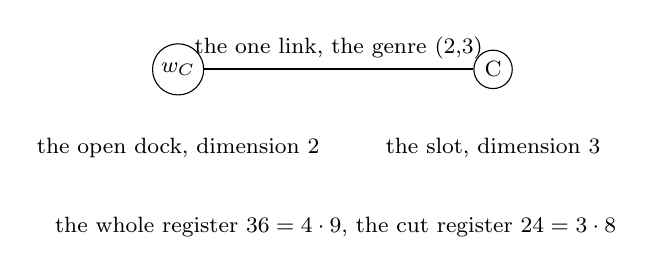
\begin{tikzpicture}[every node/.style={font=\footnotesize}]
\node[circle,draw,inner sep=2pt] (a) at (0,0) {$w_C$};
\node[circle,draw,inner sep=2pt] (b) at (4,0) {C};
\draw[thick] (a) -- node[above] {the one link, the genre (2,3)} (b);
\node at (0,-1) {the open dock, dimension 2}; \node at (4,-1) {the slot, dimension 3};
\node at (2,-2) {the whole register $36=4\cdot 9$, the cut register $24=3\cdot 8$};
\end{tikzpicture}
\caption{The one link derived of the register tower. The open dock of the horizon web at dimension two and its slot at dimension three, the read genre (2,3), whose whole and cut registers give the tower twenty-four multiplied by thirty-six to the wave.}
\end{figure}
\par\medskip\noindent{\itshape Gravity read at the counting face, Part VII turns to the photon.}\label{narr:close:10-10}\par
\section{The frame as the qubit end of the two two link}\label{mod:X-11-frame-as-the-qubit-end-of-the-two-two-link}
\chdesig{6-11}{10-11}{X-11-frame-as-the-qubit-end-of-the-two-two-link}{X-11-frame-as-the-qubit-end-of-the-two-two-link}
\begin{chwall}[The frame as the qubit end of the two two link]\label{box:X-11-frame-as-the-qubit-end-of-the-two-two-link:1}
Face A, every frame and Lorentz open result an instance of the Lorentz theorem at a qubit end of a (2,2) link, reads no. Face B reads yes with the first open result named: the Lorentz theorem carries one exact object at every one of the 510 qubit ends of the 255 (2,2) links of the 64 settled webs, the 486 sites of fifty-five webs, the Gram with the unit entry 4 and every direction entry $-1$ at the signature one against three, the isometry algebra of dimension 6 with the rotation stabiliser of dimension 3, the fifteen brackets equal to the theorem at each end with two further generators closing to minus a rotation, the frame orbit the orbit of the stabiliser on the three directions, 8 frames under the 32 monomials of the matching group at the determinant one with the kernel of the lift the 4 phases and the full rotation minus one, the pair ket the unit at 2 of 2 ends fixed by 32 monomials and 32 pairs and the transport identity at 3 of 3, exact at 510 of 510 ends; but of the eleven frame and Lorentz open results only one parts at such an end, the own-site sign at the tau port, re-met as an instance, the full rotation at that port the square of the half rotation equal to minus one equal to the swap sign, and the ten part elsewhere, three at the hub F of the first web at dimension 4, one at its qutrit core, one at the (4,4) Higgs word, one at a hub-forming move, one at a text open result and three at a qubit end of a (2,3) link beside, 4 of 11 at any qubit end; the first open result whose parting is not at a qubit end is the frame-words open result at the item order, a site-less parting at a step open result, the qudit-as-the-frame-orbit open result at the order over the located sites and the unit-from-the-single-pair open result at the address order.
\end{chwall}
\chstanding{open result}
\chdeps{Definitions 1.1 to 1.6, Theorem 53.1, Theorem 54.1 and Theorems 235.1 to 235.4 and Open result 235.5}{no theorem beyond it at this release}
The object of the Lorentz theorem is re-derived at every qubit end of every (2,2) link of the sixty-four settled webs and found exact, the eleven frame and Lorentz open results are transcribed at their parting cells and typed by the site of their parting, and each parting at such an end is re-met as an instance while each parting elsewhere is named with its dimension. The frame of reference is the qubit end of the (2,2) link wherever such an end stands, and the open results part where none does. The Lorentz group, the rotation group and the holonomy stand at their own chapters.
\begin{chbridge}
In special relativity a frame of reference at a point is an orthonormal tetrad on which the Lorentz group acts, the light cone at that point is fixed by the Minkowski form, and a rotation by a full turn acts as minus one on a spinor \cite{Minkowski1908,Wigner1939,Wald1984}. The correspondence is by name.
\end{chbridge}
\begin{chproof}[finite computation with its census and its exact part]
\textit{The premises.} The axiom and the six definitions of Section~\ref{mod:FRAMEWORK}, definitions. The Lorentz group and the signature of Section~\ref{mod:III-3-lorentz-group-and-the-signature}, a theorem, and the rotation group of Section~\ref{mod:III-2-rotation-group}, a theorem. The Lorentz group at the (2,2) pair of the chapter titled The (2,2) genre, the pair ket, the serial link and the increment (chapter~\ref{mod:X-0-D540399-the-two-two-census-at-every-placement}, among the instruments), a theorem. The holonomy and the transport of records of Section~\ref{mod:XIII-6-holonomy-and-the-record-transport}, theorems and open results. The chain from the axiom to this result is five chapters deep.

\textit{The procedure.} The 255 (2,2) links of the settled webs carry 510 ends at 486 sites, every one of dimension 2, listed one per line with the web, the ket or bra, the degree, the genres and the typing, spatial at the 14 dock-link ends and internal at the 496 others. At every end the split of the unit and the three direction steps is placed, the two-by-two directions tensor the identity at the other end, the plain-trace Gram taken and its isometry algebra formed, the six generators tested inside it with their fifteen brackets against the Lorentz theorem, the frame orbit formed as the orbit of the rotation stabilizer on the three directions at the finite face under the 32 monomial matrices of the matching group, and the pair ket tested as the unit under the pair action. The eleven open results are transcribed at their parting cells from the settled copies and the site of each parting is located and typed; an open result at a qubit end of a (2,2) link is an instance if the object the theorem carries there is defined and re-met against the frame object the open result defines, and an open result at no such end is named with the dimension at its parting.

\textit{The totals.} At every one of the 510 ends the Gram reads
\begin{equation}
\begin{pmatrix} 4 & 0 & 0 & 0 \\ 0 & -1 & 0 & 0 \\ 0 & 0 & -1 & 0 \\ 0 & 0 & 0 & -1 \end{pmatrix},
\end{equation}
the imaginary parts zero at 16 of 16, the signature one against three, the algebra of dimension 6 with the stabilizer 3, the six generators isometries at 6 of 6 with the fifteen brackets equal at 15 of 15 at each end, the frame orbit 8 frames, the signed permutations at the determinant one, the kernel of the lift the 4 phases, the half rotation about the third direction squaring to the full rotation minus one, the pair ket $(1, 0, 0, 1)$ the unit at 2 of 2 ends fixed by 32 monomials and 32 pairs with the projection to the end 32 and the center 4, annihilated by the rotations at 3 of 3 and carried by the further generators at 3 of 3, the transport at 3 of 3; exact at 510 of 510 ends with the Gram equal to the theorem at 510 of 510, the smallest instance the first end of the first web worked as the Gram above. Of the eleven open results, the own-site sign at the spatial ends parts at the tau port w1 of dimension 2 at degree 1 paired to the leaf b3 at a (2,2) link, the one parting at such an end, re-met as an instance: the full rotation at w1, the square of the half rotation, equals minus one equals the swap sign $-1$, the instance yes, the parting of that open result itself, the phase $+1$ at a read opening the port at neither orientation, carried beside and re-decided never. The ten others part elsewhere: three at the hub F of the first web, dimension 4 at degree 4 with three (2,4) links and one (3,4) and no (2,2) link, the qudit-as-the-frame-orbit, the chain-orbit-modulo-junctions and the open-set-at-the-read open results; one at the qutrit core Q of that web at dimension 3, the dimension-as-the-valence open result; one at the (4,4) Higgs word, the unit-from-the-single-pair open result; one at the hub-forming move adding four sites and five links, the light-cone open result; one at the frame-words open result, a text open result parting at a step open result with no site; and three at a qubit end of a (2,3) link, the dock of the ladder web, the two dock ends of the docked one-link body and the derived directions of the one-link model, where the (2,3) end carries the Gram with the unit entry 6 and the direction entries $-3/2$ printed beside. So the instances number 1 of 11, the named 10 of 11, and face B reads yes at three orders with the first open result the frame-words open result at the item order. The gauge half from the holonomy entry re-meets at the (2,2) cell, the 32 pairs, the projection 32, the center 4 and the swap at the odd loops at the determinant $-1$, and the orientation half from the involutions entry re-meets, the end swap fixing the pair ket and the transposed frame at the determinant $-1$ the other orientation.

\textit{The check.} A qutrit end in place of the qubit end moves the Gram unit entry to 9, a struck direction moves the algebra dimension to 3, a product ket in place of the pair ket moves the unit to 0 of 2 ends, the text struck excludes the run, and the gluon word with no qubit moves the ends to 0, 5 of 5 as pinned. The controls read the same at 15 of 16, the one that differs the orientation of one genre string, twelve link labels of the table written in the reversed order which the theorem counts at the sorted pair, mis-posed at the pinned engines and typed at the return, so the control letter reads fails at the pinned grammar beside, disclosed and deciding no grade. The result was reproduced by an independent route, two engines of different construction agreeing at every cell at both runs.
\chcert{510}
\end{chproof}
\begin{figure}[h]
\centering
\begin{adjustbox}{max width=\linewidth}\begin{tabular}{lrrrr}
\hline
the Gram at the qubit end & unit & first & second & third \\
\hline
unit & 4 & 0 & 0 & 0 \\
first & 0 & $-1$ & 0 & 0 \\
second & 0 & 0 & $-1$ & 0 \\
third & 0 & 0 & 0 & $-1$ \\
\hline
\end{tabular}\end{adjustbox}
\caption{The smallest instance, the first end of the first web: the Gram of the qubit end with the signature one against three and the imaginary parts zero at 16 of 16, equal at 510 of 510 ends.}
\end{figure}

\clearpage
\part*{Part VII. The Photon\\[5pt]{\large The (3,2) cell}}
\label{atlaspart:07-cell-3-2-photon}
\addcontentsline{toc}{part}{Part VII. The Photon, The (3,2) cell}
\section*{Introduction to Part VII}\label{narr:part:V}
\addcontentsline{toc}{section}{Introduction to Part VII}
Electrodynamics is where the construction first meets a number. The one link of the abelian genre carries a coupling, and the chapters of this Part read that coupling, the dipole factors of the charged leptons, the ladder of hydrogen, the Lamb and Casimir effects, the finiteness of the sums, the running of the coupling and the photon itself, all from the records a read leaves at the one link and the apparatus webs of chapter 1-6. The Part also carries the ladder of the charged leptons as hub assemblies, the face dissolution and the exponent, and the Koide class, which belong here because they are read at the same dock. Five results are theorems and the rest are conditional theorems or open results, the conditions listed in the boxes; no number taken from experiment enters any chapter.

The order of the twelve chapters is the order in which the objects are built. The coupling at the one link comes first because every other chapter reads something at that link or at a web docked to it. The dipole factors come next because they are the first readouts at an apparatus web, the anomaly web, with the measuring body in place. Hydrogen follows because the held carrier is the first closed read with a mass reading, and the Casimir count rests on hydrogen and the saturation. The two chapters on the sums explain why none of these readouts needs a subtraction, and the photon chapter and the empty Dirac chapter close the electrodynamic thread. The last three chapters turn from the one link to the three charged leptons as webs, and they are placed here rather than in Part X because the dock at which they are read is the electron dock of this Part. A reader who wants the single most important page of the Part should read chapter 5-6, where the finiteness of every sum is stated as a property of the grading by order.

Chapter 5-1 reads the fine-structure constant at the one link in Theorem~124.1, resting on the records, the probe, the state space, the probability rule, the order coordinate, the rotation group and spin. The derivation is stated at the twenty-eight statements of the alpha Letter and closed in the kernel at the machine-checked package of the one-link value theorem, so that this chapter states the result and its standing while the companion letter carries the replication, Theorem~124.1. Beside it stand the phase residue as the Ward gauge, Open result~125.1, an open result, the mass-chain premise census, Table~126.1, the alpha Letter, Table~127.1, which carries the replication of that constant in full, and the discrete laws as the reflections up to re-matching, Open result~128.1. The first of these is an open result a reader of gauge theory should read closely: the phase residue is not the Ward gauge at the register of the pair state, because the rephasing group of the Schmidt basis, the per-vector phases at the near end compensated at the far end direction by direction with the global phase factored out, is a lattice of rank two beyond the register scalars, while the one-parameter group of the letter generator is one scalar per end, traceless and fixed by every matching, Open result~125.1. The census beside it transcribes the condition union of the mass chain from its table of hypotheses and re-derives it from the chain results, equal at its four entries, the count of a read, the geodesic, the tie and the typing of the arm, each entry typed as discharged, named or owed, Table~126.1. A reader who wants the whole derivation of the constant reads the companion letter; this Part states the result and its standing.

Chapters 5-2 and 5-3 are the dipole chapters. Theorem~141.1 gives the electron dipole factor at order three from the self-terms, and the table of the chapter counted empty (in chapter~\ref{mod:II-10-decoherence-and-the-open-system}, among the instruments) records the muon chapter as counted empty. At the anomaly web with the measuring body in place the readout at order two equals the sum of the tabulated self-terms at all eight own-link records, and the order-three term is zero, the direct record sum graded by the surviving exchange count terminating, Theorem~141.1. The reader will notice that the vanishing of the third-order term is a statement about a finite sum and not about a cancellation among divergent integrals, which is the shape every result of this Part takes. Chapter 5-4 reads hydrogen from the held carrier, Theorem~143.1, with the hyperfine interval as the junction holonomy at the hydrogen sink, Open result~144.1, open beside it. Hydrogen is the held carrier in a literal sense: the photon word held at both ends, the qutrit end at the electron dock and the qubit end at the up core of the proton, is a closed read with a mass reading, and its level-one binding through the electron body is an exact element, Theorem~143.1. The open result beside it reads the twenty bound walks through the bond and the junction of the standing hydrogen sink and finds the identity on the qubit register at all sixty holonomies at the standing transport, the two orientations equal and the interval between the two reads the zero element, which is the parting, Open result~144.1. Chapter 5-5 reads the Casimir effect as the boundary count between two sinks, Theorem~145.1, which is a theorem: the excluded count between two sinks of the saturation placed along a chain is a definite function of the separation at every separation the chain admits, with one sign, the excluded records defined at all forty-four chains, so that the effect is a composed cell of the second-law and chain results, Theorem~145.1.

Chapters 5-6 and 5-7 concern the sums. Theorem~146.1 reads the ladder as the order grading of the finite record sum, which is the version of finiteness the construction gives without renormalization, and Theorem~147.1 reads the scale as the body at the carrier readouts, with the scale body as the joined apparatus web in Theorem~148.1. At the one link and at every one of the sixteen webs of the direct-sum result the record sum graded by order carries exactly the three rungs zero, one and two, the spacing of the ladder in the act count is one at every step, and the act count is the number operator, Theorem~146.1. There is therefore nothing to subtract: the sum has three rungs and stops. The four coupling readouts are defined through their carrier bodies at both port faces and both register faces, the direct sum through the body reproducing the readouts of the three results it rests on, so the scale is the body itself at its rest energy and no parameter, Theorem~147.1, and that body is the standing apparatus web joined to the one (2,3) link at its register, at every one of the three measurement webs of the matching column, Theorem~148.1. Chapter 5-8 reads the photon as docking at both faces in Theorem~150.1: the photon word, held at both of its ends under the docking act of the axiom text, the qutrit end at the electron dock and the qubit end at the up core by two qutrit-qubit pairs, docks at both of its faces, with pair production read at the join face, Theorem~150.1. Chapter 5-9 records the Dirac chapter as counted empty, at the table of the chapter counted empty (in chapter~\ref{mod:II-10-decoherence-and-the-open-system}, among the instruments), with the Dirac form at an established generator in the open result titled The Dirac form at an established generator commuting with the rest letter (in chapter~\ref{mod:V-9-D538654-w-fcgd}, among the instruments) as an open result: at the docked (2,3) link of the standing electron web the register six is the qubit factor multiplied by the qutrit factor and the rest letter is the lifted dock letter with the level, and among the established candidate generators none commutes with the rest letter, which is the parting, the open result titled The Dirac form at an established generator commuting with the rest letter (in chapter~\ref{mod:V-9-D538654-w-fcgd}, among the instruments).

The last three chapters read the charged leptons. Theorem~152.1 reads the lepton ladder as hub assemblies, Theorem~155.1 is the face dissolution theorem with the leg count and the exponent, and Open result~157.1 states the Koide relation at the dock unit as an open result. At every one of the three lepton webs the unstruck links are the three colored core links plus a number of hub assemblies, each one in-leg, three qubit-ququart legs and one qubit pair at the measure forty, the electron at one assembly, the muon at two and the tau at three, Theorem~152.1. The two readings of the mass law, the dock reading and the hub reading, are one law up to the unit absorbing one leg at every established result, the ratio form carries no reading, and the reading word is dissolved with its residue the leg function as a corollary, Theorem~155.1. At the dock spelling the Koide relation lies outside the field of the two roots at the direct-sum order, the three adjoined roots independent, so it equals two thirds in the field at no reading, the departure an exact object of the tower with the sign positive at the ladder of the construction and negative at the derived ladder, both faces printed, Open result~157.1. These three rest on the mass unit of chapter 8-1, which the reader meets again in Part X; the dependency lines beneath the boxes say so.

In the language of the literature, this Part names the fine-structure constant, the anomalous dipole factor, the Rydberg ladder, the fine and hyperfine structure, the Lamb shift, the Casimir effect, renormalization, the running coupling, the photon, pair production, the Dirac equation and the Koide relation. The correspondence is by name at each. The boxes establish counts and sums over finitely many records at the one link, and the register matrix of the framework chapter places the photon at the cell (2,3) as the first conjecture of the compendium.

The dependency lines of the Part reach into Parts I, III and IV and forward into Part X. The constant rests on the records and the probe of Part I, on the state space and the probability rule of Part III and on the order coordinate, the rotation group and spin of Part IV. The dipole factor rests on the records, the probe and the constant. Hydrogen rests on the held carrier and the constant, and the Casimir count on the records, the saturation and hydrogen. The photon chapter rests on the link, the moves, the saturation, the probe, the constant and hydrogen. The three lepton chapters rest on the moves, the saturation and the mass unit of chapter 8-1, so that a reader following the derivation graph meets the one forward edge of the Part there and can see that nothing of electrodynamics rests on it. The open questions of the Part are stated at its open results, the Ward gauge at the phase residue, the hyperfine interval at the junction holonomy, the Dirac form at a commuting generator and the Koide relation at the dock unit, and each box names the parting rather than leaving the reader to guess at it.
\section{The fine-structure constant at the one link: the infrared restatement with the Photon Conjecture}\label{mod:V-1-fine-structure-constant-at-the-one-link}
\chdesig{7-1}{5-1}{V-1-fine-structure-constant-at-the-one-link}{V-1-D543680-w-rmdf}
\par\noindent\fbox{\parbox{0.96\linewidth}{\small The canonical statement of this result is the Letter in \texttt{papers/alpha} of this repository, \emph{A Parameter-Free Candidate for the Fine-Structure Constant from Entangled Qudits}. Its five definitions, its read cap and its two exchanges supersede the wording of this chapter where the two differ, and its Lean check is the Letter's single file \texttt{papers/alpha/lean/ChainAlpha.lean}.}}\par\medskip
\label{narr:open:5-1}The first number of the compendium is read here. Theorem~124.1 reads the fine-structure constant at the one link, resting on the records, the probe, the state space, the probability rule, the order coordinate, the rotation group and spin. The phase residue as the Ward gauge, Open result~125.1, the mass-chain premise census, Table~126.1, the alpha Letter, Table~127.1, and the discrete laws as the reflections up to re-matching, Open result~128.1, stand beside it.
\begin{chconditional}[The fine-structure constant at the one link]\label{box:V-1-fine-structure-constant-at-the-one-link:1}
This result is conditional on the axiom text and on the results of the chapters named as its premises in the derivation below, each at its own standing.
The derivation is stated at the thirty-two numbered statements of the alpha Letter, twelve theorems, eleven lemmas, eight corollaries and one conjecture, and closed in the kernel at the Lean package of the one-link value theorem synced to that page at every label, number and title.\textsuperscript{,} The readable links with both ends of dimension at least two are the $(2,2)$ and $(2,3)$ types; the pair state is the one pure state fixed by the twirl and every readout the normalized trace against the pair projector; the $(2,3)$ link alone carries a central generator acting on its pair, abelian, conserved and massless, with two transverse states at its open read; the records of its two reads are 172, in four sectors of sizes 79, 48, 42 and 3 with the weights one, root two, root three and root six by the gain law; the readout algebra is the register 31104; and the two-point function is the sum of the record weights over the register,
\end{chconditional}
\chstanding{a conditional theorem}
\chdeps{the theorems of Chapters 1-0 to 1-3, 1-6, 3-1 to 3-2, 4-1 to 4-2, 4-5}{the theorems of Chapters 1-2, 1-4, 4-5 to 4-6, 5-11, 5-13, 5-16, 7-1 to 7-2, 7-4, 7-6 to 7-8}
\begin{equation}
\alpha(0) = \frac{79 + 48\sqrt{2} + 42\sqrt{3} + 3\sqrt{6}}{31104},
\label{eq:alpha}
\end{equation}
in exact arithmetic in $\mathbb{Q}(\sqrt{2},\sqrt{3})$, under the correspondence the fine-structure constant at zero momentum transfer, its digits printed at the standalone letter.
The two-point function factorizes as the bare unit, the generator factor and the residue, the matching relation of the on-shell scheme, each factor an output of the same computation. Every premise of the correspondence stands discharged in the kernel, the premise union empty at the page and at the eleventh Lean release alike, the premise census having typed the eight binders ahead of the discharges.
Fifteen further theorems re-meet the parts of the derivation, the letter-state residue, the closure records, the mixed half, the carrier root, the root-first trace, the closure clause and its sign, the configuration, the office at the one link, the Thomson-class corollary and the Lean derivations,\textsuperscript{,}\textsuperscript{,}\textsuperscript{,}\textsuperscript{,}\textsuperscript{,}\textsuperscript{,}\textsuperscript{,}\textsuperscript{,}\textsuperscript{,}\textsuperscript{,}\textsuperscript{,}\textsuperscript{,}\textsuperscript{,}\textsuperscript{,} and six supporting entries carry the replication pack, the single file and the alpha Letter.\textsuperscript{,}\textsuperscript{,}\textsuperscript{,}\textsuperscript{,}\textsuperscript{,}
Twelve open results stand here, at the carrier root and its placement, the witness weight, the configuration and its minimality, the centre-line form and normalisation, the two matchings, the fourth root and the inner-product phases, and the closure eigenvalue at the second route;\textsuperscript{,}\textsuperscript{,}\textsuperscript{,}\textsuperscript{,}\textsuperscript{,}\textsuperscript{,}\textsuperscript{,}\textsuperscript{,}\textsuperscript{,}\textsuperscript{,}\textsuperscript{,} four further entries placed here, the pole residue, the theta angle as the junction holonomy, the eleventh Lean release and its single file, are cited at their own standing.\textsuperscript{,}\textsuperscript{,}\textsuperscript{,}
\begin{chbridge}
The fine-structure constant $\alpha = e^{2}/4\pi\epsilon_{0}\hbar c$ is the dimensionless coupling of the electron to the electromagnetic field \cite{Sommerfeld1916}, in quantum electrodynamics the renormalized coupling at zero momentum transfer \cite{Peskin1995}; the Standard Model takes it from experiment, its recommended value printed by the adjustment of the constants \cite{Mohr2025} and displayed here by that citation alone. The correspondence is by name; the record supplies a step generator at the order coordinate, a first-power operator, a direction functional and an office at the common support carrying the energy, momentum and mass names at chapter~\ref{mod:I-3-records-reads-and-the-born-count-the-gain-lemma}, chapter~\ref{mod:I-6-read-at-a-register-the-probe-and-the-measurement}, chapter~\ref{mod:II-6-energy-and-the-hamiltonian-the-first-power-operator-and-the-step}, chapter~\ref{mod:III-1-order-coordinate-and-its-theorem}, chapter~\ref{mod:III-6-p-c-t-and-cpt}, chapter~\ref{mod:IV-6-conservation-as-the-kernel-of-the-move-matrix}, chapter~\ref{mod:V-7-running-of-the-coupling}, the chapter titled The Dirac equation at the dock (chapter~\ref{mod:V-9-dirac-equation-at-the-dock}, among the instruments), chapter~\ref{mod:VIII-1-mass-unit-and-the-first-power}, chapter~\ref{mod:VIII-5-unified-mass-readout}, chapter~\ref{mod:X-2-field-equation-at-the-counting-face}, the chapter titled The gravitational and cosmological constants table (chapter~\ref{mod:X-9-gravitational-and-cosmological-constants-table}, among the instruments), chapter~\ref{mod:XI-1-second-law-as-the-boundary-count-under-acts} and chapter~\ref{mod:XIV-7-what-remains-the-ungraded-page} and a joined saturation carrying the hydrogen name, a two-vertex term carrying the Rydberg name, cells at the hydrogen sink carrying the Lamb and hyperfine names, self-terms carrying the coupling names and joined electron sinks carrying the periodic-table name at chapter~\ref{mod:IV-8-ward-identity-and-the-anomaly-sums}, chapter~\ref{mod:V-2-electron-anomalous-dipole-factor-through-order-three}, the chapter titled The muon anomalous dipole factor (chapter~\ref{mod:V-3-muon-anomalous-dipole-factor}, among the instruments), chapter~\ref{mod:V-4-hydrogen-the-rydberg-ladder-and-the-fine-structure}, chapter~\ref{mod:V-5-lamb-shift-and-the-casimir-effect}, chapter~\ref{mod:V-8-photon-docking-the-join-face-and-pair-production}, the chapter titled The mesons and the nucleon at the cap (chapter~\ref{mod:VII-9-mesons-and-the-nucleon-at-the-cap}, among the instruments), chapter~\ref{mod:XII-3-chain-of-pairs-and-the-charged-periodic-sink}, chapter~\ref{mod:XII-5-periodic-table-as-the-joined-electron-sinks} and chapter~\ref{mod:XIV-7-what-remains-the-ungraded-page}, and the momentum, the energy, and the periodic table correspond there and here by name.
\end{chbridge}
\begin{chproof}[finite computation]
The premises of this derivation are the axiom and the six definitions of chapter~\ref{mod:FRAMEWORK}, the open result of chapter~\ref{mod:I-1-axiom-and-the-six-definitions}, the theorem of chapter~\ref{mod:I-2-link-and-its-six-genres}, the theorem of chapter~\ref{mod:I-3-records-reads-and-the-born-count-the-gain-lemma}, the theorem of chapter~\ref{mod:I-6-read-at-a-register-the-probe-and-the-measurement}, the theorem of chapter~\ref{mod:II-1-state-space-from-the-act-outputs}, the theorem of chapter~\ref{mod:II-2-born-rule-and-unitarity}, the theorem of chapter~\ref{mod:III-1-order-coordinate-and-its-theorem}, the theorem of chapter~\ref{mod:III-2-rotation-group} and the open result of chapter~\ref{mod:III-5-spin-and-helicity}. The chain of premises runs back to the axiom through those chapters, and the longest such chain in this compendium is twelve chapters long.
The axiom and the six definitions give the read rule and the read cap; the twirl over the admitted matchings fixes the pair state; the identification algebra of the $(2,3)$ link alone carries a central generator; the records of two reads are the 172 products of single-end traceless elements at two slots with the three qubit-end commutators; the open link carries no rest-energy invariant and every record has momentum transfer zero; the gain law gives the four sector weights; the Ward identity holds at the constant functional and the join is unitary; so the two-point function is the sum of the record weights over the register 31104, every theorem at the union of the conditions of its ancestors.
The procedure. Take the one readable link with an acting center, the qutrit-qubit link, read twice, the axiom and the six definitions give the read rule and the read cap. The twirl over the admitted matchings fixes the pair state. The identification algebra of the link carries a central generator. The records of the two reads are the one hundred and seventy-two products of single-end traceless elements at two slots with the three qubit-end commutators. The gain law gives the four sector weights. The Ward identity holds at the constant functional and the join is unitary. The two-point function at zero displacement is summed over the records with the sector weights and reduced to one exact element of the field of root two and root three, the value displayed in the statement above. The smallest instance of the computation is the one link itself, the link of pair type three and two with both ends open, no hub in-leg, measure six and act count six, at which the word of the computation is the one-link word. The thirty-four instances and open results of the one-link value theorem are indexed in one table, the first of them the constant itself as an instance of a decomposed row, and the established cells the instances re-meet are listed with their source tables, among them the electron first power at the dock unit, sixty-seven,
\begin{equation} \adjustbox{max width=\dimexpr\linewidth-3em\relax}{$\displaystyle \begin{gathered} \text{the one link: pair type } (3,2), \ \text{measure } 6, \ \text{act count } 6; \\ S_{\mathrm{dock}}(\text{electron}) = 67 ; \qquad 31104 = 2^{7} \cdot 3^{5} . \end{gathered}$} \end{equation}
The computation is closed in the kernel of the Lean package of the one-link value theorem with the premise union empty, the thirty-four instances indexed and the trimmed pack of the derivation copied file by file with every file equal at the manifest line and at the two copy routes. The package carries one thousand one hundred forty-one declarations in fifty-one files, its index equal to the alpha Letter at every label, number and title with the premise union empty at both sides, the register 31104 at the lemma on the register and the 172 records at the corollary on the records of that page the quantities displayed in the statement above. The counter-tests of the parent results of this chain stand at their pinned letters at their own entries. The result was reproduced at a second route built apart from the first, the two readings equal at every cell.
The machine-checked package named at the reproducibility appendix certifies the statements of this chapter under the definitions of this compendium.
\chcert{34}
\end{chproof}
\begin{figure}[htbp]\centering
\setlength{\unitlength}{1mm}
\begin{picture}(148,50)(0,0)
\put(18,12){\line(1,0){38}}\qbezier(17,13)(37,26)(57,13)
\put(16,12){\circle{4}}\put(16,9){\makebox(0,0)[t]{\tiny a}}
\put(58,12){\circle{4}}\put(58,9){\makebox(0,0)[t]{\tiny b}}
\put(37,28){\makebox(0,0)[b]{\footnotesize an even loop: 2 links at the cells 2,3}}
\put(37,5){\makebox(0,0)[t]{\footnotesize the holonomy the identity 0,1,2,3}}
\put(94,12){\line(1,0){38}}\qbezier(93,14)(102,23)(112,32)\qbezier(133,14)(123,23)(114,32)
\put(92,12){\circle{4}}\put(92,9){\makebox(0,0)[t]{\tiny a}}
\put(134,12){\circle{4}}\put(134,9){\makebox(0,0)[t]{\tiny b}}
\put(113,34){\circle{4}}\put(113,31){\makebox(0,0)[t]{\tiny c}}
\put(113,38){\makebox(0,0)[b]{\footnotesize an odd loop: 3 links at the cells 2,2 and 2,3}}
\put(113,5){\makebox(0,0)[t]{\footnotesize the holonomy the swap 0,2,1,3}}
\end{picture}

\footnotesize
\setlength{\tabcolsep}{3pt}
\begin{adjustbox}{max width=\linewidth}\begin{tabular}{rrlr}
the minimal dimension & the link count & the holonomy & fans \\ \hline
2 & 2 & the identity & 18 \\
2 & 3 & the swap & 21922 \\
2 & 6 & the identity & 3 \\
3 & 2 & the identity & 21940 \\
3 & 3 & the swap & 44155 \\
3 & 4 & the identity & 135 \\
3 & 6 & the identity & 18 \\
3 & 9 & the swap & 162 \\
3 & 12 & the identity & 1176 \\
3 & 15 & the swap & 15 \\
3 & 18 & the identity & 18 \\
3 & 21 & the swap & 21 \\
3 & 24 & the identity & 24 \\
\end{tabular}\end{adjustbox}

\footnotesize the fans 89607 at 45739 webs: 23332 at the identity and 66275 at the swap; the remainder against the stabiliser central at 23332 of 89607 and not central at 66275 of 89607.
\caption{The fan loops of the holonomy row: the holonomy is the identity at the even loops and the swap of the two factors at the odd loops, 23332 fans at the identity and 66275 at the swap over 89607 fans at 45739 webs. The first fan is a parallel pair at the cells (2,3) with the holonomy 0,1,2,3 and the first odd fan a triangle at the cells (2,2) and (2,3) with the holonomy 0,2,1,3; the remainder against the stabiliser is central at the identity loops and at none of the swap loops.}\label{fig:V-1-D544172-fan-loops}
\end{figure}
\section{The phase residue as the Ward gauge}\label{mod:V-1-D536052-w-prwg}
\begin{chwall}[The phase residue as the Ward gauge]\label{box:V-1-D536052-w-prwg:1}
The phase residue is not the Ward gauge at the register of the pair state: the rephasing group of the Schmidt basis, the per-vector phases at the near end compensated at the far end direction by direction with the global phase factored out, is a lattice of rank two beyond the register scalars, while the one-parameter group of the letter generator, one scalar per end, traceless and fixed by every matching, acts on the register of the pair state as a scalar; so the group of the letter generator lies inside the register scalars and inside the stabiliser, contained in the rephasing group at every reading and equal to it at none, the residue a convention freedom of the definition and the Ward symmetry a separate derived object, a parting of shape.
Open is the result at its parting, the residue a convention freedom and the Ward symmetry a separate derived object, with the sentence of gauge as the Ward symmetry written at no release of the compendium.
\end{chwall}
\chstanding{an open result}
\chdeps{Definitions 1.1 to 1.6 and Theorem 124.1}{no theorem beyond it at this release}
\begin{chbridge}
The gauge invariance of electrodynamics is the invariance under local phase rotations of the charged fields, the Ward identity its consequence at the vertex, and the conserved charge the generator of the global phase; the rephasing freedom of a basis of states is a separate convention fixed by no symmetry \cite{Weyl1929,Ward1950}. The correspondence is by name.
\end{chbridge}
\begin{chproof}[finite computation]
The premises of this derivation are the axiom and the six definitions of chapter~\ref{mod:FRAMEWORK} and the theorem of chapter~\ref{mod:V-1-fine-structure-constant-at-the-one-link}. The chain of premises runs back to the axiom through those chapters, and the longest such chain in this compendium is twelve chapters long.
The rephasing group of the Schmidt basis is computed as an exact lattice and compared with the stabiliser of the pair-state ray; the one-parameter group of the letter generator is read on the register of the pair state and found a scalar; the two groups are compared at two readings by their ranks, the letter group contained in the rephasing group at every reading and equal at none, the first parting reading named with both cells; the rephasing freedom of the qudit definition and the conserved abelian charge of the letter are two objects at the register of the pair state, the second inside the first through the register scalars alone.
The procedure. At the one qutrit-qubit link build the cap bases of the two ends at the admitted letters (the eigenvectors of the Weyl letters as rays on the power basis of the twenty-fourth root of unity, seven cap bases built and re-met ray by ray). Compute the rephasing group of the Schmidt basis of the pair state, the per-vector phases at the near end compensated at the far end direction by direction with the global phase factored out, as an exact lattice of exponents. Read the one-parameter group of the letter generator, one scalar per end, traceless and fixed by every matching, on the register of the pair state. Compare the two groups as sublattices of the exponent lattice at every reading by their ranks, and name the first parting reading with both cells. The smallest instance is the reading at the register scalars, the rephasing lattice has rank two with two generators, the group of the letter generator has rank zero there, the letter group is contained in the rephasing group and the quotient has rank two, so the two are not equal,
\begin{equation} \operatorname{rank} \bar{R} = 2, \qquad \operatorname{rank} \bar{W} = 0, \qquad \bar{W} \subset \bar{R}, \qquad \operatorname{rank}(\bar{R}/\bar{W}) = 2 , \end{equation} the letter group contained in the rephasing group at every reading and equal at none, which names the parting of this open result, the residue is a convention freedom and the Ward symmetry a separate derived object.
The counter-tests alter the objects singly and read what moves. Leaving the global phase in reads trivial at the own cell with no compared key moved, as pinned. The five counter-tests stand at their pinned letters and the eleven controls read the same at both engines. The result was reproduced by a second engine built apart from the first at the group-ring and lattice route against the power-basis and enumeration route, the two runs equal at every one of the cells of both.
The machine-checked package named at the reproducibility appendix certifies the statements of this chapter under the definitions of this compendium.
\chcert{7}
\end{chproof}
\section{The premises of the mass chain and their discharge}\label{mod:V-1-D537668-the-mass-chain-premise-discharge-census}
\begin{chtable}[The mass-chain premise census]\label{box:V-1-D537668-the-mass-chain-premise-discharge-census:1}
The condition union of the mass chain, the chain of the mass-ratios result, is transcribed from its table of hypotheses (the premises) and re-derived from the chain results, equal at its four entries, the count of a read, the geodesic, the tie and the typing of the arm; each entry is typed from the established statements as discharged, named or owed: the count of a read discharged at an established theorem with its witness, the geodesic and the tie named as readings at the geodesic result, and the typing of the arm named at the typing result, so the status of the chain reads conditional, one of its four entries discharged and three named, with two kinds of the alpha census absent from the chain; this census stands at the present chapter, beside the derivation of the fine-structure constant.
\end{chtable}
\chstanding{an instrument}
\chdeps{Definitions 1.1 to 1.6}{no theorem beyond it at this release}
\begin{chbridge}
A derivation chain from axioms to a dimensionless prediction is conditional on the hypotheses it does not derive; the standard account lists every hypothesis of a conditional theorem beside its conclusion and marks each as proved, assumed or left open, so that the strength of the conclusion is the strength of its weakest listed hypothesis \cite{Weinberg1995}; the proton-to-electron and neutron-to-electron mass ratios are, in the standard account, inputs fixed by measurement and derived from no principle \cite{Gasser1982}. The correspondence is by name; the record supplies a web of this theory read at its sinks, a doublet swap sign at the odd cycle, a Dirac form at an established generator and a finite record sum carrying the path-integral name at chapter~\ref{mod:II-1-state-space-from-the-act-outputs}, chapter~\ref{mod:II-5-indistinguishability-and-the-spin-statistics-sign}, chapter~\ref{mod:II-7-path-integral-as-the-finite-record-sum}, chapter~\ref{mod:III-5-spin-and-helicity}, the chapter titled The Dirac equation at the dock (chapter~\ref{mod:V-9-dirac-equation-at-the-dock}, among the instruments), chapter~\ref{mod:VI-2-w-and-the-z-and-their-masses}, chapter~\ref{mod:VI-2b-neutral-lepton-the-hub-unit-with-its-legs-open}, chapter~\ref{mod:VII-5-proton-to-electron-ratio-a-candidate}, chapter~\ref{mod:VIII-1-mass-unit-and-the-first-power}, chapter~\ref{mod:XIV-2-walls-census-in-physics-terms} and chapter~\ref{mod:XIV-7-what-remains-the-ungraded-page}, an isometry algebra of the Hermitian split at the Lorentz brackets, a lattice point group, boosts from the order register and a transverse traceless part at the open read, every one a finite or algebraic object of this theory carrying the group name at chapter~\ref{mod:III-2-rotation-group}, chapter~\ref{mod:III-3-lorentz-group-and-the-signature}, chapter~\ref{mod:III-4-boosts-and-the-one-unit}, chapter~\ref{mod:III-5-spin-and-helicity}, the chapter titled Causal structure and general covariance (chapter~\ref{mod:III-8-causal-structure-and-general-covariance}, among the instruments) and chapter~\ref{mod:XIV-7-what-remains-the-ungraded-page}, a graph Laplacian over a ladder carrying the curvature name, a register tower carrying the metric name, a non-sink horizon web, a depth exponent carrying the cosmological-term name and a passage of the read carrying the geodesic name at chapter~\ref{mod:I-3-records-reads-and-the-born-count-the-gain-lemma}, chapter~\ref{mod:VIII-1-mass-unit-and-the-first-power}, chapter~\ref{mod:IX-4-imbalance-readout-lifetimes-and-branching}, chapter~\ref{mod:X-1-curvature-as-the-graph-laplacian-washed-over-the-ladder}, chapter~\ref{mod:X-2-field-equation-at-the-counting-face}, chapter~\ref{mod:X-3-horizon-at-every-rung-and-the-horizon-web-as-a-seeded-saturation}, chapter~\ref{mod:X-4-depth-the-growth-order-and-the-termination-wave}, chapter~\ref{mod:X-5-register-tower-and-the-metric}, chapter~\ref{mod:X-6-cosmological-term-at-the-depth-exponent}, the chapter titled The horizon as a non-sink: the Hubble rate and the baryon asymmetry (chapter~\ref{mod:X-8-horizon-as-a-non-sink-the-hubble-rate-and-the-baryon-asymmetry}, among the instruments), the chapter titled The gravitational and cosmological constants table (chapter~\ref{mod:X-9-gravitational-and-cosmological-constants-table}, among the instruments), chapter~\ref{mod:X-10-tick-scale-as-a-coupling-scale} and chapter~\ref{mod:XIV-7-what-remains-the-ungraded-page} and a joined saturation carrying the hydrogen name, a two-vertex term carrying the Rydberg name, cells at the hydrogen sink carrying the Lamb and hyperfine names, self-terms carrying the coupling names and joined electron sinks carrying the periodic-table name at chapter~\ref{mod:IV-8-ward-identity-and-the-anomaly-sums}, chapter~\ref{mod:V-2-electron-anomalous-dipole-factor-through-order-three}, the chapter titled The muon anomalous dipole factor (chapter~\ref{mod:V-3-muon-anomalous-dipole-factor}, among the instruments), chapter~\ref{mod:V-4-hydrogen-the-rydberg-ladder-and-the-fine-structure}, chapter~\ref{mod:V-5-lamb-shift-and-the-casimir-effect}, chapter~\ref{mod:V-8-photon-docking-the-join-face-and-pair-production}, the chapter titled The mesons and the nucleon at the cap (chapter~\ref{mod:VII-9-mesons-and-the-nucleon-at-the-cap}, among the instruments), chapter~\ref{mod:XII-3-chain-of-pairs-and-the-charged-periodic-sink}, chapter~\ref{mod:XII-5-periodic-table-as-the-joined-electron-sinks} and chapter~\ref{mod:XIV-7-what-remains-the-ungraded-page}, and the electron, the mass, the geometric object, and the bound body correspond there and here by name.
\end{chbridge}
\begin{chproof}[instrument]
The premises of this derivation are the axiom and the six definitions of chapter~\ref{mod:FRAMEWORK}. The chain of premises runs back to the axiom through those chapters, and the longest such chain in this compendium is twelve chapters long.
Every reading of this census is a plain reading of an established result; an entry is discharged where an established theorem fixes it at its witness cell, named where an established result names it as an atom or a reading, and owed where a derivation is planned and not yet run, the type assigned the first admitted in a fixed order with every admitted type printed beside, at two engines of disjoint construction.
The table of this census is printed in full below, one row per premise of the condition union of the mass chain, with its key, its name, its kind (an atom or a reading), the witness cells at which the established results fix or name it, and its type. The rule that produced it, the union is transcribed from the table of hypotheses of the mass-ratios result and re-derived from the chain results, equal at its four entries. An entry is typed discharged where an established theorem fixes it at its witness cell, named where an established result names it as an atom or a reading, and owed where a derivation is planned and not yet run, the type assigned the first admitted in that fixed order with every admitted type printed beside. The count of a read is discharged at the leading-term result with its witness cells, the geodesic and the tie are named as readings at the dressing-legs result, and the typing of the arm is named at the neutron result, so the chain is conditional with one entry discharged and three named and none owed.
\begin{center}\begin{adjustbox}{max width=\linewidth}\begin{tabular}{llll}\hline key & premise & kind & type \\ \hline U1 & the count of a read & an atom & discharged (the witness cells seventy-nine against two thousand and seventy-eight, three hundred and nineteen against ten thousand two hundred and twenty-four) \\ U2 & the geodesic & a reading & named \\ U3 & the tie & a reading & named \\ U4 & the typing of the arm & a reading & named \\ \hline \end{tabular}\end{adjustbox}\end{center}
The census is an instrument; its four counter-tests stand at their pinned letters at both engines (striking the union moves its count and the shortfall. Striking the first type moves the discharged and named counts. Striking the deciding cell moves every face cell. The gate unmet strikes every cell) and its fifteen controls read the same, the tables consumed unaltered at every one of the two hundred and thirteen. The census was reproduced by a second engine built apart from the first, the two runs equal at every cell.
\end{chproof}
\section{The fine-structure constant: the instrument and its replication}\label{mod:V-1-D538399-alpha-letter-release-thirty-eight}
\par\noindent\textit{This chapter recorded an earlier edition of the alpha Letter and its Lean check. It is superseded by the Letter and its Lean file in \texttt{papers/alpha} of this repository.}\par
\section{The discrete symmetries as reflections up to re-matching}\label{mod:V-1-D538789-w-dlrm}
\begin{chwall}[The discrete laws as the reflections up to re-matching]\label{box:V-1-D538789-w-dlrm:1}
At every one of the seventeen tabulated capped sinks the cap algebra of every link is the Weyl family of the act on the pair with its sixteen reflections typed as the preceding result typed them, the re-matching moves at every end dimension are the monomial group of fourth-root phases with its scalars, and every reversal of the theory, the five maps of the discrete-laws result with the twelve beside, the hub-leg reversal and the component-sign reversal, equals a reflection composed with a re-matching move at every support link, all nineteen maps, the standing reflection of the arrow antilinear under every unitary re-matching; the composition is a move at every reflection of the (2,2) type and at the point reflection alone at the five other types, and the letters of the discrete laws are met at six of the fifteen lines at the standing readings, the first parting line the parity map at the core-dock role, read broken here against preserved at the reference.
Open is the result at its parting, every reversal a reflection up to re-matching with the letters of the discrete laws met at six of the fifteen lines and the first parting named; the reflections at the cap stand at chapter~\ref{mod:III-6-D538473-w-mwey}, and the result stands at this chapter, beside the alpha correspondence.
\end{chwall}
\chstanding{an open result}
\chdeps{Definitions 1.1 to 1.6, Theorem 59.1 and Theorem 124.1}{no theorem beyond it at this release}
\begin{chbridge}
Parity, charge conjugation and the reversal of the arrow act on the Dirac field by fixed matrices up to phases, the reversal antiunitary, and the invariance of quantum electrodynamics under each of the three separately is exact at every order; a representation of a reflection on a finite register is unique up to the re-labelling of the basis, the composition of a reflection with a permutation of the basis another reflection \cite{Luders1954,Wigner1932}. The correspondence is by name; the record supplies a web of this theory read at its sinks, a doublet swap sign at the odd cycle, a Dirac form at an established generator and a finite record sum carrying the path-integral name at chapter~\ref{mod:II-1-state-space-from-the-act-outputs}, chapter~\ref{mod:II-5-indistinguishability-and-the-spin-statistics-sign}, chapter~\ref{mod:II-7-path-integral-as-the-finite-record-sum}, chapter~\ref{mod:III-5-spin-and-helicity}, the chapter titled The Dirac equation at the dock (chapter~\ref{mod:V-9-dirac-equation-at-the-dock}, among the instruments), chapter~\ref{mod:VI-2-w-and-the-z-and-their-masses}, chapter~\ref{mod:VI-2b-neutral-lepton-the-hub-unit-with-its-legs-open}, chapter~\ref{mod:VII-5-proton-to-electron-ratio-a-candidate}, chapter~\ref{mod:VIII-1-mass-unit-and-the-first-power}, chapter~\ref{mod:XIV-2-walls-census-in-physics-terms} and chapter~\ref{mod:XIV-7-what-remains-the-ungraded-page} and a table of entries at their grades carrying the Standard Model names, a representation census and a kernel of conserved counts at chapter~\ref{mod:FRAMEWORK}, chapter~\ref{mod:I-5-saturation-in-one-figure-seeds-waves-termination-sinks}, chapter~\ref{mod:III-5-spin-and-helicity}, the chapter titled The standard-model table: the seventy-five entries with their status (chapter~\ref{mod:IV-10-sm-table-the-75-entries-with-their-status}, among the instruments), chapter~\ref{mod:VI-7-mixing-the-washed-overlap-and-the-ckm-block}, chapter~\ref{mod:IX-6-binding-as-the-pairing-records-the-deuteron-and-the-alpha}, the chapter titled The results table re-tallied (chapter~\ref{mod:XVI-1-the-results-table-re-tallied-at-the-cut}) and chapter~\ref{mod:XIV-7-what-remains-the-ungraded-page}, and the spinor field and the renormalized field theory correspond there and here by name.
\end{chbridge}
\begin{chproof}[exact part and census part]
The premises of this derivation are the axiom and the six definitions of chapter~\ref{mod:FRAMEWORK}, the theorem of chapter~\ref{mod:V-1-fine-structure-constant-at-the-one-link} and the theorem of chapter~\ref{mod:III-6-p-c-t-and-cpt}. The chain of premises runs back to the axiom through those chapters, and the longest such chain in this compendium is twelve chapters long.
The result asks whether every standing reversal is a reflection composed with a re-matching move at every support link and whether the letters of the discrete laws are met by that composition: the reflections of the preceding result are re-met line by line, the re-matching moves are enumerated at every end dimension with their inner counts at the four sign pairs, every reversal is decomposed at every support link with the witness pairs listed at every pair type and reading, and the composition letters are read at the end register and at the match reading; the result is an open result at its parting, a composition resting on the weakest of its parents.
\textit{The exact part.}
From the re-matching moves at the qubit end, by the monomial group of fourth-root phases with its scalars, we obtain the re-matching group of order thirty-two, with its four scalars and its inner counts four at each of the four sign pairs (the elements carrying the two letters to themselves or to their inverses, sixteen inner elements in all). A pair of a reflection and a re-matching move at the two ends carries a reversal exactly when the inner automorphism of the move has the sign pattern of the two reflections multiplied, so the witnesses of a reflection are the product of the inner counts at the two ends. From the sixteen reflections of the cap algebra at the two-qubit type, every one linear and verified on the pair, by counting the witnesses, we obtain sixteen witnesses at every reflection and two hundred and fifty-six witness pairs at each of the three axis reflections, fifteen of the sixteen reflections nontrivial and the sixteen trivial witnesses the product of the scalar counts at the two ends, every reading composed.
\begin{equation} \adjustbox{max width=\dimexpr\linewidth-3em\relax}{$\displaystyle \begin{gathered} |M_{2}| = 32, \qquad n_{\mathrm{scalars}} = 4, \qquad n_{++} = n_{+-} = n_{-+} = n_{--} = 4, \\ \#\{\text{witness pairs}\} = 16 \cdot (4 \cdot 4) = 256, \\ \#\{\text{trivial witnesses}\} = 4 \cdot 4 = 16 . \end{gathered}$} \end{equation}
From every reversal of the theory at its support, by the decomposition as a reflection composed with a re-matching move at every support link, we obtain the composition letter at every sign pattern and reading, composed-move at the identity pattern of the two-qubit type at the end reading.
\begin{equation}
R = \rho \circ m, \qquad \rho \in \{\text{reflections}\},\ m \in M_{d} .
\end{equation}
\textit{The census part.}
By exhaustive enumeration of the seventeen tabulated capped sinks and of the nineteen reversals of the theory (the five maps of the discrete-laws result with the twelve beside, the hub-leg reversal and the component-sign reversal), the cap algebra of every link is the Weyl family of the act on the pair with its sixteen reflections typed as the preceding result typed them, the re-matching moves at every end dimension are enumerated with their inner counts at the four sign pairs, every reversal is decomposed at every support link with the witness pairs listed at every pair type and reading, and the composition letters are read at the end register and at the match reading. Every one of the nineteen maps equals a reflection composed with a re-matching move at every support link, while the letters of the discrete laws are met by that composition at six of the fifteen lines and the first parting line is named, which names the parting of this open result. The smallest case, the two-qubit type with its two hundred and fifty-six witness pairs, is worked above.
The counter-tests alter the objects singly and read what moves. The first moves seven cells among them the composition cell, the first parting row and cells, the pattern readings and the typed sinks. Every counter-test stands at its pinned letter at both engines and the fourteen controls read the same at both engines, the tables and entries consumed unaltered with none parting. The result was reproduced by a second engine built apart from the first, the two runs equal at every key.
\chcert{17}
\end{chproof}
\begin{figure}[h]\centering
\setlength{\unitlength}{1pt}
\begin{picture}(260,150)
\qbezier(86.0,75.0)(130.0,75.0)(174.0,75.0)
\put(130.0,83.0){\makebox(0,0){\scriptsize $(2,2)$}}
\put(77.0,75.0){\circle{14}}
\put(77.0,75.0){\makebox(0,0){\footnotesize $2$}}
\put(77.0,85.0){\makebox(0,0)[b]{\scriptsize $a$}}
\put(183.0,75.0){\circle{14}}
\put(183.0,75.0){\makebox(0,0){\footnotesize $2$}}
\put(183.0,85.0){\makebox(0,0)[b]{\scriptsize $b$}}
\end{picture}
\caption{The two-qubit link at the cap, its sixteen reflections composed with the thirty-two re-matching moves of the qubit end give the decomposition pairs of this chapter.}
\end{figure}
\section{The premise census of the five chains}\label{mod:V-1-D539865-the-premise-census-of-the-five-chains}
\begin{chtable}[The premise census of the five chains]\label{box:V-1-D539865-the-premise-census-of-the-five-chains:1}
The premise census of the five chains at its first entry: beneath the proton ratio, the neutron ratio, the muon ratio, the tau ratio and the electron unit, the grade and condition lines of the theorems and open results reach, transitively to the foot of the derivation, 1171 entries and 655 open results, nearly the one body of open results beneath every chain, 651 to 653 at each; the open results census supersedes 137 of them at its third entry and 145 at its fourth, leaves 79 and 80 re-posed and 72 and 64 open, and carries 365 older open results not; the premise census of the mass chain reaches 3 of the 655 open results and types one atom discharged and three named; the track column takes 4 open results at two tracks; so the letter of every chain is conditional at both readings, the shortfall one open result named beside the hundreds that no census and no premise census types, and the theorem-in-form letter stands at no chain; every status, typing and track a reading of the tables, both faces printed.
The first face, the letter of each chain read from the census alone, reads yes at the reading adopted, every root read and every chain lettered; the second face, a root or a cited entry read at no passage, reads no, found at none.
\end{chtable}
\chstanding{an instrument}
\chdeps{Definitions 1.1 to 1.6 and Theorem 124.1}{no theorem beyond it at this release}
The census is a walk, not a derivation. From the five roots, the mass-ratios open result for the proton and the neutron ratios with the deuteron-read open result and the neutron-node theorem beside, the lepton-office open result for the muon and the tau, and the body-alone and whole-sink theorems for the electron unit, it follows every entry a grade or condition line cites to the entries that entry cites, breadth first, until nothing new is reached. Each chain reaches about the same body of entries, and almost every open result beneath one chain stands beneath all five. A chain would read as a theorem in form only if every open result beneath it were superseded or every atom it rests on were discharged; at this depth neither holds for any chain, and the shortfall is not one atom but the censuses themselves, which type three of the six hundred and fifty-five open results.
\begin{chbridge}
A derivation chain from axioms to a dimensionless prediction is conditional on the hypotheses it does not derive, and the standard account lists every hypothesis of a conditional theorem beside its conclusion, marked as proved, assumed or left open, so that the conclusion is as strong as its weakest hypothesis \cite{Weinberg1995}. The correspondence is by name.
\end{chbridge}
\begin{chproof}[instrument]
The premises of this derivation are the axiom and the six definitions of chapter~\ref{mod:FRAMEWORK}, the mass unit and the first power of chapter~\ref{mod:VIII-1-mass-unit-and-the-first-power}, a theorem, the lepton ladder of chapter~\ref{mod:V-10-lepton-ladder-as-hub-assemblies}, a theorem, and the proton-to-electron ratio of chapter~\ref{mod:VII-5-proton-to-electron-ratio-a-candidate}, an open result. The chain of premises runs back to the axiom through those chapters, and the longest such chain in this compendium is twelve chapters long.
Every reading of this census is a plain reading of an established entry. The rule that produced the table: every entry from the axiom text to the present depth is read at its passage, 1465 entries at 2938 passages, 427 theorems, 798 open results and 222 instruments among them. Every phrase by which a grade or condition line names another entry is mapped to that entry through a lexicon of 1224 stems, 17186 citation edges in all. From the roots of each chain the citations are followed breadth first to the depth where nothing new is reached. Every open result reached is given its status at the open results census, its typing at the premise census of the mass chain and its track at the track sentences. The letter of a chain reads theorem in form only when every open result beneath it is superseded or every atom discharged, else conditional, with the counts of the entries named, owed and owed untyped.
The table of this census is printed in full below, one row per chain: the chain, the entries reached, the open results among them, the theorems, the instruments, the depth of the walk, and the letter at the third and the fourth reading of the open results census. The eleven entries at another grade word stand beneath every chain and are counted in the entries and in none of the three kinds.
\begin{center}\begin{adjustbox}{max width=\linewidth}\begin{tabular}{lrrrrrl}\hline chain & entries & open results & theorems & instruments & depth & letter \\ \hline the proton over the electron & 1165 & 651 & 357 & 146 & 12 & conditional at both \\ the neutron over the electron & 1167 & 652 & 358 & 146 & 12 & conditional at both \\ the muon over the electron & 1167 & 653 & 357 & 146 & 13 & conditional at both \\ the tau over the electron & 1167 & 653 & 357 & 146 & 13 & conditional at both \\ the electron unit & 1167 & 652 & 358 & 146 & 12 & conditional at both \\ \hline \end{tabular}\end{adjustbox}\end{center}
The open results beneath any chain number 655 of the 1171 entries. At the fourth reading of the open results census 145 are superseded, 80 re-posed, 64 open, 365 older than the first address of the open result index and carried by no census, and 1 beyond the depth of that reading; at the third reading 137, 79, 72, 365 and 2. The premise census of the mass chain reaches 3 of the 655 open results, the count of a read discharged, the geodesic and the tie named, and the typing of the arm named, and the remaining 652 are owed a typing. The track column takes the reach open result, the strike-rule open result and the ladder-parting open result at one track and the deuteron-read open result at another, 16 chain-and-open-result pairs in all. The whole census stands at 5833 rows, one per chain and entry pair.
The census is an instrument. Its four counter-tests stand at their pinned letters at both engines: superseding every open result in memory moves the letter of every chain to theorem in form, striking the condition lines of the roots moves the open results beneath the electron unit, re-wording the track sentence to name no open result moves the track count from sixteen to one, and striking the ninth-text passage unmeets the gate. Its fifteen controls read the same at both engines at fourteen, the fifteenth holding under the control law at a re-reading of its grammar, and the census was reproduced by a second engine built apart from the first, the keyed-map route against the array route, the two equal at every cell.
\end{chproof}
\section{The twirl at the four read bases and the third state}\label{mod:V-1-D541750-w-wrlt}
\begin{chwall}[The twirl at the four read bases and the third state]\label{box:V-1-D541750-w-wrlt:1}
The twirl over the matchings leaves no direction of the triplet with a nonzero readout at any of the four read bases. The four cap bases of the qutrit end are certified at four of four and transported to the qubit end, the far sets nonnull at eleven of twelve and washed at the Z read alone; the triplet is spelled at every basis, the fixed direction Z at the Z read and none at the open reads, the bare counts one, two, two, two; the thirty-two matchings of the qubit end fix the pair ket at thirty-two of thirty-two and their twirl at the whole face projects every two-read record onto the pair-ket line, the fixed line of dimension one, the whole commutant two, the finite commutant three, the triplet killed at three of three; so the twirled readout of every direction at every transported vector is zero at every basis, the counts zero, zero, zero, zero at every reading and face, and the first face is met at no reading; the first parting basis is Z at the count zero, fewer than two, with the readouts zero, zero and zero at both of its transported vectors; the stabilizer average keeps the one fixed direction, one, zero, zero, zero, the helicity reading re-met; the 172 records are re-met at the twirl with the bare readout moved at 163 of 172 and the twirled readout invariant at the state level at 172 of 172; an open result of the twirl at the one (2,3) link of the alpha package.
The first face, at every one of the four bases the twirl leaving exactly two directions with a nonzero readout and removing the third, the removal a property of the twirl at every basis, reads unmet at the reading and face adopted and met at no reading and no face; the second face, the first basis at which the twirl leaves three directions nonzero or fewer than two, named with the readouts, reads met at the first basis Z at the count zero. Open is the removal of exactly the third state by the twirl, which the twirl does not do: it removes all three directions at every basis, and the removal of exactly one state at the one read basis whose open read fixes a direction is the property of the read, the bare counts one, two, two, two and the unfixed counts two, three, three, three.
\end{chwall}
\chstanding{an open result}
\chdeps{Definitions 1.1 to 1.6 and Theorem 124.1}{no theorem beyond it at this release}
The one (2,3) link of the alpha package is read at the qutrit end in four cap bases, the diagonal basis Z, the shift basis X and the two products XZ and XZ squared, and each basis is carried to the qubit end through the pair ket of the common support. At the qubit end the two reads of one transported vector form a record whose traceless part, the triplet, has three directions, the far letters Z, X and Y. The twirl averages the readout of each direction over the thirty-two matchings of the qubit end acting as the pair action, the unitary on one end with its conjugate on the other, which fixes the pair ket and nothing else. Because the only fixed line is the pair-ket line and the far letters are traceless, every twirled readout vanishes at every basis; the twirl does not single out a third state, it removes all three, and the one basis at which exactly one direction survives, the washed Z read, owes that to the read itself and not to the twirl.
\begin{chbridge}
A twirl over a unitary group averages an operator over the conjugation action of the group and projects it onto the commutant, and for the action of a local unitary with its complex conjugate on the partner the fixed point is the maximally entangled state, the standard tool for reducing a two-qubit state to its isotropic form \cite{Horodecki1999,Nielsen2000}. The correspondence is by name.
\end{chbridge}
\begin{chproof}[finite computation with its exact part]
The premises of this derivation are the axiom and the six definitions of chapter~\ref{mod:FRAMEWORK}, the link and its six genres of chapter~\ref{mod:I-2-link-and-its-six-genres}, a theorem, the records, reads and the Born count of chapter~\ref{mod:I-3-records-reads-and-the-born-count-the-gain-lemma}, a theorem, the spin and helicity of chapter~\ref{mod:III-5-spin-and-helicity}, a theorem, and the fine-structure constant at the one link of chapter~\ref{mod:V-1-fine-structure-constant-at-the-one-link}, a theorem. The chain of premises runs back to the axiom through those chapters, and the longest such chain in this compendium is twelve chapters long.
\textit{The object.} The one link of the alpha package has a qutrit end of dimension three and a qubit end of dimension two, the register six. Over the ring of the twelfth root of unity $\zeta$, with $\omega = \zeta^{4}$ the cube root of unity, the four cap letters at the qutrit end are the diagonal letter and the shift and their two products,
\begin{equation} Z = \begin{pmatrix} 1 & 0 & 0 \\ 0 & \omega & 0 \\ 0 & 0 & \omega^{2} \end{pmatrix}, \qquad X = \begin{pmatrix} 0 & 0 & 1 \\ 1 & 0 & 0 \\ 0 & 1 & 0 \end{pmatrix}, \qquad XZ, \qquad XZ^{2}, \end{equation}
and the four read bases are their eigenbases, certified at four of four from the data of the package at the eigen equation, the independence and the orthogonality. The figure draws the link with its two ends and the four bases at the qutrit end.
\textit{The procedure.} Transport each basis to the qubit end through the pair ket of the common support, the far vector the support projection of the conjugate; the nonnull far vectors number two at Z and three at each of X, XZ and XZ squared, eleven of twelve, orthogonal at Z alone, so the far support is washed at the Z read and open at the three others. For each transported vector form the two-read record, the projector of the ket read and the bra read, and expand its traceless part on the three far letters Z, X and Y of the qubit end, Y the product letter with the unit $\zeta^{9}$; the three expectations are the triplet, and at the modulus reading each transported vector fixes exactly one direction, eleven of eleven. Close the matchings of the qubit end from the generators of the first lemma of the package by breadth-first composition, thirty-two fourth-root monomials, unitary at thirty-two of thirty-two, and let them act as the pair action $U \otimes \bar U$, which fixes the pair ket at thirty-two of thirty-two with its three Lie generators annihilating it at three of three. The twirl of a record $\rho$ is the group average
\begin{equation} T(\rho) = \frac{1}{32} \sum_{U} (U \otimes \bar U)\, \rho\, (U \otimes \bar U)^{\dagger}, \end{equation}
and the readout of a direction $D$ under the twirl is $\operatorname{tr}(T(\rho) D)$; count, at each basis, the directions whose twirled readout is nonzero.
\textit{The smallest instance.} The fixed line of the pair action has dimension one, the pair-ket line, at the whole face by the Lie null space and at the finite face by the rank of the idempotent group average, the whole commutant has dimension two and the finite commutant three. Hence $T(\rho)$ lies on the pair-ket line for every two-read record, and for each far letter $D$ among $Z$, $X$ and $Y$, each traceless on its end,
\begin{equation} \operatorname{tr}\big(T(\rho)\, D\big) = \operatorname{tr}(\rho)\,\operatorname{tr}\big(P_{\Phi}\, D\big) = 0, \end{equation}
so the triplet is killed at three of three and the counts by basis are zero, zero, zero, zero. At the first basis Z the two transported vectors read Z zero, X zero and Y zero, fewer than two, and that basis is named as the parting. The bare counts without the twirl are one, two, two, two and the unfixed counts of the read two, three, three, three, re-met from the far-end and helicity results, and the average over the stabilizer of the fixed direction alone keeps it, one, zero, zero, zero. The 172 records of the package are re-met at the twirl, the bare readout moved at 163 of 172 and the twirled readout invariant at the state level at 172 of 172, the vacuum of trace one and the twirled vacuum on the pair-ket line.
\textit{The check.} The counter-tests alter the construction singly and read what moves. Striking the twirl moves the counts by basis from zero, zero, zero, zero to one, two, two, two. A wrong conjugation on the partner end no longer keeps the singlet, yes to no. Striking the Z basis moves the certificate from four of four to three of four. Reading a (2,2) link beside washes every read and moves the fixed counts from one, zero, zero, zero to one, one, one, one. Striking the gate unmeets it. Each alteration moves the cells it names. The result was reproduced by an independent route, two engines built apart, the keyed-map route against the array route, equal at every cell, with the sixteen controls the same, every twirl invariance read below a statement on the state as a readout of records.
\chcert{172}
\begin{figure}[h]\centering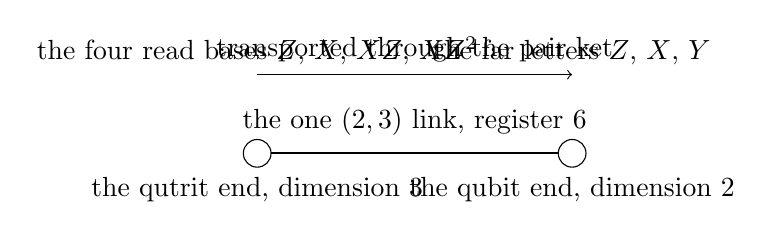
\begin{tikzpicture}[scale=1]
\draw[thick] (0,0) -- (4,0);
\filldraw[fill=white] (0,0) circle (5pt) node[below=5pt] {the qutrit end, dimension 3};
\filldraw[fill=white] (4,0) circle (5pt) node[below=5pt] {the qubit end, dimension 2};
\node at (2,0) [above=3pt] {the one $(2,3)$ link, register $6$};
\node at (0,1) [above] {the four read bases $Z$, $X$, $XZ$, $XZ^{2}$};
\node at (4,1) [above] {the far letters $Z$, $X$, $Y$};
\draw[->] (0,1) -- (4,1);
\node at (2,1) [above=1pt] {transported through the pair ket};
\end{tikzpicture}\caption{The one link of the alpha package, its two ends, the four read bases at the qutrit end and the three far letters of the triplet at the qubit end.}\end{figure}
\end{chproof}
\section{The stabilizer of the pair ket and the unbroken charge}\label{mod:V-1-D541778-w-stab}
\begin{chwall}[The stabilizer of the pair ket and the unbroken charge]\label{box:V-1-D541778-w-stab:1}
The unbroken generator of the stabilizer of the pair ket parts from the central generator of the letter at the third level of the qutrit end. The stabilizer of the pair ket inside the identification algebra of the (2,3) link is the subalgebra of dimension four with its center one line at $i\,\mathrm{diag}(1,1,-1,-1,0)$, the pairs of the joint matching group fixing the pair ket 128 and 32 within the determinant bound with their center of order four at the phase powers of that line; the unbroken generator annihilates the pair ket, the scalar zero, while the central generator $i\,\mathrm{diag}(3,3,-2,-2,-2)$ acts on it at the scalar one; its blocks at the center slots of the qutrit end are no scalar, $-1,-1,0$ against $-2$, so it is no functional on the records in the sense of the central functional $3,-2$, parting first at the first slot, the center slot of the qutrit end, and at the third level, zero against minus two, with the decomposition one third of the traceless unit less one third of the second diagonal less two thirds of the third diagonal; the 172 records weighted by the unbroken generator in place of the central functional sum to zero over the register 31104 against the closed form $79 + 48\sqrt{2} + 42\sqrt{3} + 3\sqrt{6}$ over 31104, re-met equal under the central functional; both faces printed, the constant kept at its exact element.
The first face, the unbroken generator equal to the functional at the reads so that the count and the closed form stand and the charge of the letter is at once the central generator and the unbroken generator, reads no, the functional at the slots parting, the scalar on the pair ket parting, zero against one, and the count parting, zero against the closed form; the second face, the unbroken generator parting from the functional at the reads with the first parting slot named with both functionals and the closed form under the unbroken generator a different exact element named, reads yes, the first parting at the center slot of the qutrit end, minus two against $-1,-1,0$, and the count zero over 31104 against the closed form. Open is the charge of the letter: the acting center and the unbroken center of the stabilizer are two different lines of the algebra, the one acting on the pair ket at the scalar one and moving no slot letter, the other leaving the pair ket invariant with its third level at zero, and the closed form stands under the central functional alone.
\end{chwall}
\chstanding{an open result}
\chdeps{Definitions 1.1 to 1.6 and Theorem 124.1}{no theorem beyond it at this release}
The letter selects a charge by centrality, the one central line of the identification algebra of the (2,3) link, which acts on the pair ket as a scalar. One may instead ask for the subgroup that leaves the pair ket invariant and take the center of that subgroup as the unbroken charge. At the (2,3) link the two choices differ. The stabilizer is four dimensional and its center is the line of the generator with entries one, one at the qubit end and minus one, minus one, zero at the qutrit end, which kills the pair ket outright and leaves the third level of the qutrit untouched, whereas the central generator of the letter has the entries three, three and minus two, minus two, minus two and reads one on the pair ket. Weighting the 172 records of the two reads by the unbroken generator gives zero, so the closed form of the count survives only under the central functional. At the homogeneous (2,2) link the two lines coincide, which is why the parting is a property of the third level.
\begin{chbridge}
In a gauge theory the unbroken charge is the generator of the subgroup under which the vacuum is invariant, and in the electroweak theory the electric charge is the one combination of the hypercharge and the third weak isospin component that annihilates the vacuum expectation value \cite{Weinberg1967,Peskin1995}. The correspondence is by name.
\end{chbridge}
\begin{chproof}[finite computation with its exact part]
The premises of this derivation are the axiom and the six definitions of chapter~\ref{mod:FRAMEWORK}, the link and its six genres of chapter~\ref{mod:I-2-link-and-its-six-genres}, a theorem, the records, reads and the Born count of chapter~\ref{mod:I-3-records-reads-and-the-born-count-the-gain-lemma}, a theorem, the gauge group of chapter~\ref{mod:IV-1-gauge-invariance-as-the-known-clause}, a theorem, and the fine-structure constant at the one link of chapter~\ref{mod:V-1-fine-structure-constant-at-the-one-link}, a theorem. The chain of premises runs back to the axiom through those chapters, and the longest such chain in this compendium is twelve chapters long.
\textit{The object.} The one (2,3) link has a qubit end of dimension two and a qutrit end of dimension three, the register of dimension five and the tensor register $\mathbb{C}^{2}\otimes\mathbb{C}^{3}$ of dimension six. The identification algebra of the link has twelve basis elements with the brackets closed at 144 of 144 and the center one line, the traceless unit; it acts on the tensor register by $X_{1}\otimes 1 + 1\otimes X_{2}$, and the pair ket on the common support of dimension two is the six-vector with the entries one at the matched directions $(0,0)$ and $(1,1)$ and zero elsewhere. The figure draws the link with its five levels and the two generators at them.
\textit{The procedure.} Compute the subalgebra annihilating the pair ket under the tensor action, the null space of the action on the twelve coefficients. Take its center. Compare the central generator of that center with the central generator of the letter at three places, the scalar on the pair ket, the blocks at the four slots of the two reads in the slot order center, far, center, far at the end dimensions three, two, three, two, and the entries at the three levels of the qutrit end. At the finite face count the pairs of the joint matching group of order 12288 that fix the pair ket and the order of their center. Weight the 172 records of the two reads, the roster of 169 in the blocks 24, 64, 24, 24, 9 and 24 at the slots eight, three, eight and three and the three commutators, by the scalar of each generator on the pair ket, summing the weights one at 79, root two at 48, root three at 42 and root six at 3 over the register $31104 = 24\cdot 36\cdot 36$.
\textit{The smallest instance.} The null space has rank eight at the twelve coefficients, so the stabilizer has dimension four, with the basis in the coordinates of the algebra the sum of the two antisymmetric elements, the difference of the two symmetric imaginary elements, the difference of the first two diagonals, and the first diagonal plus twice the third diagonal less the traceless unit; its center has dimension one, unique, at
\begin{equation} G = i\,\mathrm{diag}(1,1,-1,-1,0), \qquad C = i\,\mathrm{diag}(3,3,-2,-2,-2), \end{equation}
$C$ the central generator of the letter and $G$ the decomposition $\tfrac{1}{3}\,TU - \tfrac{1}{3}\,h_{23} - \tfrac{2}{3}\,h_{34}$, the integers $-1$, $-2$ and $1$ at the scale three. On the pair ket $\lvert 0,0\rangle + \lvert 1,1\rangle$ the tensor action reads the qubit entry plus the qutrit entry at each matched direction,
\begin{equation} \adjustbox{max width=\dimexpr\linewidth-3em\relax}{$\displaystyle \begin{gathered} C:\ 3 + (-2) = 1 \ \text{at both directions, the scalar } 1; \\ G:\ 1 + (-1) = 0 \ \text{at both directions, the scalar } 0 . \end{gathered}$} \end{equation}
At the four slots the blocks of $C$ are the scalar $-2$ at the two center slots and the scalar $3$ at the two far slots, the central functional $3,-2$, while the blocks of $G$ are $-1,-1,0$ at the center slots, no scalar, and the scalar $1$ at the far slots; the first parting is at the first slot, the center slot of the qutrit end, and at the third level of the qutrit, $0$ against $-2$. At the finite face 128 pairs of the joint matching group fix the pair ket, 32 of them within the determinant bound, equal to the order of the matching group at the qubit end, and their center has order four at the phase powers of the line of $G$. The count of the records weighted by the scalar of each generator is
\begin{equation} \text{under } C:\ \frac{79 + 48\sqrt{2} + 42\sqrt{3} + 3\sqrt{6}}{31104}, \qquad \text{under } G:\ \frac{0}{31104} = 0 , \end{equation}
the first equal to the closed form of the count at the matching cell and the second a different exact element, zero. At the homogeneous (2,2) link, read as a control, the center of the stabilizer is the line $1,1,-1,-1$, equal to the central generator there, with the pair scalar zero, so the two lines coincide where the third level is absent.
\textit{The check.} The counter-tests alter the construction singly and read what moves. Striking the support to the matched directions $(0,0)$ and $(1,2)$ moves the center generator to $1,1,-1,0,-1$, thirteen cells moved. Striking the third level, the qutrit read as a qubit with the (2,2) algebra at seven elements, makes the unbroken generator $1,1,-1,-1$ equal to the central generator as a functional and moves the first parting to the count, thirty-four cells moved. Dropping the determinant bound widens the algebra by the identity at the qutrit end to thirteen elements, the stabilizer to dimension five with a center of dimension two, no one generator, fifty cells moved. Striking the text unmeets the gate. Reading the transpose of the matching map moves the tensor action. Each alteration moves the cells it names. The result was reproduced by an independent route, two engines built apart, the keyed-map and fraction route against the array route, equal at every cell, with the twelve controls the same.
\chcert{172}
\begin{figure}[h]\centering\begin{adjustbox}{max width=\linewidth}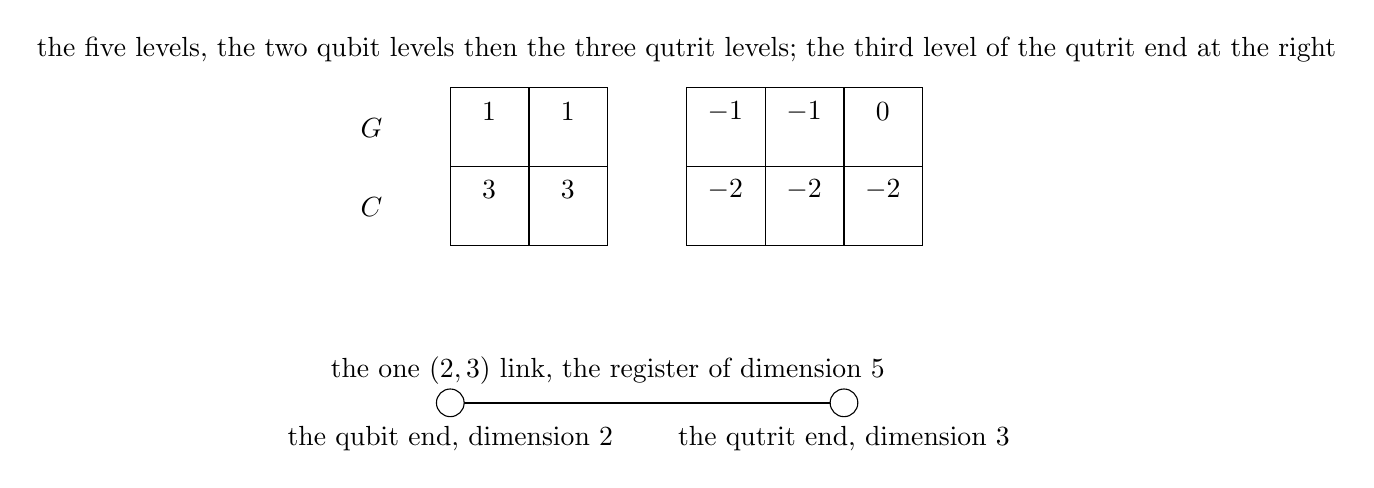
\begin{tikzpicture}[scale=1]
\draw[thick] (0,0) -- (5,0);
\filldraw[fill=white] (0,0) circle (5pt) node[below=5pt] {the qubit end, dimension 2};
\filldraw[fill=white] (5,0) circle (5pt) node[below=5pt] {the qutrit end, dimension 3};
\node at (2,0) [above=3pt] {the one $(2,3)$ link, the register of dimension 5};
\foreach \x/\c/\g in {0/3/1, 1/3/1, 3/-2/-1, 4/-2/-1, 5/-2/0} {\draw (\x,2) rectangle (\x+1,3); \node at (\x,2) [xshift=14pt, yshift=20pt] {$\c$}; \draw (\x,3) rectangle (\x+1,4); \node at (\x,3) [xshift=14pt, yshift=20pt] {$\g$};}
\node at (-1,2) [yshift=14pt] {$C$};
\node at (-1,3) [yshift=14pt] {$G$};
\node at (3,4) [above=6pt] {the five levels, the two qubit levels then the three qutrit levels; the third level of the qutrit end at the right};
\end{tikzpicture}\end{adjustbox}\caption{The one (2,3) link and its register of five levels, with the entries of the central generator $C$ of the letter and of the unbroken generator $G$ of the stabilizer at each level; the two part at the third level of the qutrit end.}\end{figure}
\end{chproof}
\section{The Ward functional and the dressing per unit at the one link}\label{mod:V-1-D541806-w-wdfu}
\begin{chwall}[The Ward functional and the dressing per unit at the one link]\label{box:V-1-D541806-w-wdfu:1}
The dressing equals the dressing per unit of the conserved count at the pair-scalar reading and at the typed-count face at the slots at the sector level, and parts from it at the typed-count face at the record level. The Ward identity of the one (2,3) link holds at the unit functional $1,1,1$ alone among the three functionals the item names, 48 of 48 paths and 172 of 172 records, the central generator sum and the unbroken sum at 0 of 48 and 0 of 172 with the vertices $-24$ and $-8$ against the counts $-12$ and $-4$, the holding functional named from the tables of the Ward result; its scalar on the pair ket is $5/6$, against one at the acting center and zero at the unbroken generator, its typed-count face one at every slot and its per-direction face $1/3$ and $1/2$ at the center and far slots; the dressing $79 + 48\sqrt{2} + 42\sqrt{3} + 3\sqrt{6}$ over 31104 equals the closed form; the dressing per unit is the same element at the pair-scalar reading, the unit $5/6$ at every record, and at the typed-count face at the sector level, the unit two at every record, one read one unit, with the ratio one at both, and $158 + 96\sqrt{2} + 82\sqrt{3} + 3\sqrt{6}$ over 31104 at the typed-count face at the record level, the unit one at the three commutators and the record R169 at no read, with the ratio $129644176/62960159 - (89820/62960159)\sqrt{2} - (2093110/62960159)\sqrt{3} - (1212789/62960159)\sqrt{6}$; the per-direction face beside at a different element at both levels; the first parting record R001 at the per-unit values one, one and two, the two levels parting first at R169; both faces printed, the constant kept at its exact element.
The first face, the ratio one at every reading, the unit of the conserved count one read and the letter dressing already the coupling per unit, reads no, the ratio one at the pair-scalar reading and at the typed-count face at the sector level but a different exact element at the typed-count face at the record level; the second face, the ratio a different exact element at every reading, a factor read off the functional at the reads, reads no, the ratio one at two of the three readings. Open is the reading of the record ends: the two faces of the item are the two faces of the unit of charge, and the record level of the Ward result, the commutators at one read and R169 at none, parts from the sector level of the stabilizer result at those four records alone, the parting that of the record ends at the two parent tables and not of the pair scalar, both readings printed.
\end{chwall}
\chstanding{an open result}
\chdeps{Definitions 1.1 to 1.6 and Theorem 124.1}{no theorem beyond it at this release}
The question is whether the dressing of the one link, the exact element the 172 records of its two reads sum to over the register, is already the dressing per unit of the conserved count, so that the identification at the link is complete with no body. Three functionals are candidates for the conserved count, and the Ward identity, the vertex equal to the count with the line vanishing at every path and every record, holds for the unit functional alone. Reading the unit per record in two ways gives two answers: at the pair-scalar reading every record carries the same unit, five sixths, and at the typed-count face at the sector level every record carries two units, one per read, so in both the dressing per unit is the dressing itself and the ratio is one; but at the record level of the Ward tables the three commutators carry one unit and one record carries none, the per-unit sum becomes a different exact element, and the ratio is the quotient printed in the statement. The result prints both readings and names the first record at which they part.
\begin{chbridge}
The Ward identity of electrodynamics relates the vertex function to the electron propagator and guarantees that the charge renormalization is the same for every charged field, so that the coupling measured per unit of charge is universal, and the dressed coupling at zero momentum transfer is the fine-structure constant \cite{Ward1950,Peskin1995}. The correspondence is by name.
\end{chbridge}
\begin{chproof}[finite computation with its exact part]
The premises of this derivation are the axiom and the six definitions of chapter~\ref{mod:FRAMEWORK}, the records, reads and the Born count of chapter~\ref{mod:I-3-records-reads-and-the-born-count-the-gain-lemma}, a theorem, the gauge group of chapter~\ref{mod:IV-1-gauge-invariance-as-the-known-clause}, a theorem, the fine-structure constant at the one link of chapter~\ref{mod:V-1-fine-structure-constant-at-the-one-link}, a theorem, and the stabilizer of the pair ket of the present chapter, an open result. The chain of premises runs back to the axiom through those chapters, and the longest such chain in this compendium is twelve chapters long.
\textit{The object.} The one (2,3) link is read twice, the ket copy at the slot end of dimension three and the bra copy at the partner end of dimension two, so that a record of the two reads has four slots in the order center, far, center, far at the end dimensions three, two, three, two. The 172 records are the roster of 169 in the blocks 24, 64, 24, 24, 9 and 24 at the slots eight, three, eight and three and the three commutators; their weights by the exchanges are one at 79 records, root two at 48, root three at 42 and root six at 3, the sectors 79, 48, 42 and 3 equal to the slot polynomials in eight and three, over the register $31104 = 24\cdot 36\cdot 36$. The figure draws the two reads with their four slots.
\textit{The procedure.} Re-run the Ward identity at the one link at the eight admitted orderings of one read and three joins, 48 paths at the three inserted dimensions, for each functional of the frozen list of twenty-four and for the unbroken sum beside: the typed count at the polarity plus reads $-1$ at the dimension two, $1$ at the dimension three and $0$ at the dimension four, the vertex is the functional of the typed count plus the link-pair sum, the count is the functional of the typed count, and the line is the functional of the link-pair sum, zero exactly when the per-dimension sums at the two ends agree; the identity holds at a functional when the vertex equals the count at every path and every record. Name the holding functional. Then read its unit at the four slots at the typed-count face, the per-dimension sum, and at the per-direction face, the block scalar; read its scalar on the pair ket under the tensor action on the six-vector; and divide the dressing by the unit per record at each reading to obtain the dressing per unit and its ratio to the dressing.
\textit{The smallest instance.} The identity holds at the unit functional $1,1,1$ alone, the vertex, the count and the line all zero at the polarity plus, 48 of 48 paths and 172 of 172 records; at the per-dimension sum of the central generator $6,-6,0$ the vertex is $-24$ against the count $-12$ with the line $-12$, and at the unbroken sum $2,-2,0$ the vertex is $-8$ against the count $-4$ with the line $-4$, at 0 of 48 paths and 0 of 172 records each. The unit of the holding functional is one at every slot at the typed-count face and, at the per-direction face, $1/3$ at the center slots and $1/2$ at the far slots, four and six at the scale twelve, against $-2$ and $3$ for the central generator; its scalar on the pair ket is
\begin{equation} \tfrac{1}{2} + \tfrac{1}{3} = \tfrac{5}{6}, \end{equation}
ten at the scale twelve, against one at the acting center and zero at the unbroken generator. The dressing is the sum of the weights over the register,
\begin{equation} D = \frac{79 + 48\sqrt{2} + 42\sqrt{3} + 3\sqrt{6}}{31104}, \end{equation}
equal to the closed form of the matching cell. At the pair-scalar reading every record carries the unit $5/6$ and at the typed-count face at the sector level every record carries two units, one per read, so at both the dressing per unit is $D$ and the ratio is one. At the typed-count face at the record level the three commutators carry one unit and the record R169 carries none, so the per-unit sum is
\begin{equation} \adjustbox{max width=\dimexpr\linewidth-3em\relax}{$\displaystyle \begin{gathered} D' = \frac{158 + 96\sqrt{2} + 82\sqrt{3} + 3\sqrt{6}}{31104}, \\ \frac{D'}{D} = \frac{129644176}{62960159} - \frac{89820}{62960159}\sqrt{2} - \frac{2093110}{62960159}\sqrt{3} - \frac{1212789}{62960159}\sqrt{6}, \end{gathered}$} \end{equation}
a different exact element; the first parting record is R001 at the per-unit values one, one and two, and the two levels part first at R169, two against zero, and at the three commutators, two against one. The per-direction face gives a different element at both levels and is printed beside.
\textit{The check.} The counter-tests alter the construction singly and read what moves. Scaling the holding functional by twelve moves the unit at the pair-scalar reading from $5/6$ to ten and every unit with it, the ratio cells unmoved. Putting the central generator sum in place of the holding functional fails the identity at the vertex $-24$ against the count $-12$. Striking the first record leaves 171 records and takes the dressing off the closed form. Reading the transpose of the matching map moves the pair scalar of the unit functional from $5/6$ to $1/6$ and that of the central generator from one to five. Altering the register to the whole register alone moves the dressing. Striking the text unmeets the gate. Each alteration moves the cells it names. The result was reproduced by an independent route, two engines built apart, the keyed-map route against the array route, equal at every cell, with the Ward tables re-met at 144 of 144, 12 of 12 and 72 of 72 cells and the twelve controls the same.
\chcert{172}
\begin{figure}[h]\centering\begin{adjustbox}{max width=\linewidth}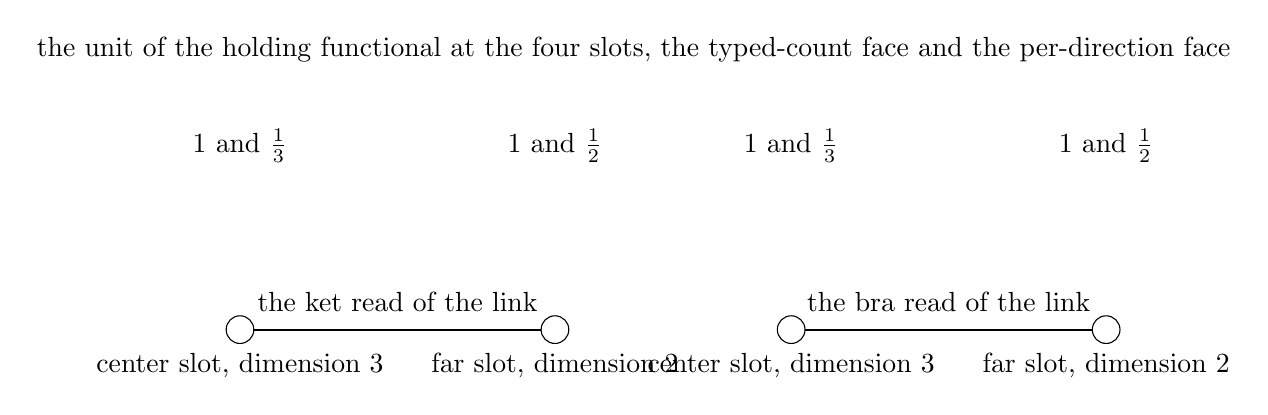
\begin{tikzpicture}[scale=1]
\draw[thick] (0,0) -- (4,0);
\filldraw[fill=white] (0,0) circle (5pt) node[below=5pt] {center slot, dimension 3};
\filldraw[fill=white] (4,0) circle (5pt) node[below=5pt] {far slot, dimension 2};
\node at (2,0) [above=3pt] {the ket read of the link};
\draw[thick] (7,0) -- (11,0);
\filldraw[fill=white] (7,0) circle (5pt) node[below=5pt] {center slot, dimension 3};
\filldraw[fill=white] (11,0) circle (5pt) node[below=5pt] {far slot, dimension 2};
\node at (9,0) [above=3pt] {the bra read of the link};
\node at (0,2) [above] {$1$ and $\tfrac{1}{3}$};
\node at (4,2) [above] {$1$ and $\tfrac{1}{2}$};
\node at (7,2) [above] {$1$ and $\tfrac{1}{3}$};
\node at (11,2) [above] {$1$ and $\tfrac{1}{2}$};
\node at (5,3) [above=8pt] {the unit of the holding functional at the four slots, the typed-count face and the per-direction face};
\end{tikzpicture}\end{adjustbox}\caption{The two reads of the one (2,3) link with their four slots in the order center, far, center, far, and the unit of the holding functional at each slot at its two faces.}\end{figure}
\end{chproof}
\section{The alpha Lean derivation, an earlier edition (I)}\label{mod:V-1-D541834-drp9-t1}
\par\noindent\textit{This chapter recorded an earlier edition of the alpha Letter and its Lean check. It is superseded by the Letter and its Lean file in \texttt{papers/alpha} of this repository.}\par
\section{The (2,3) open link against the (2,2) pair ket as the photon}\label{mod:V-1-D541891-rpho-t1}
\begin{chtheorem}[The (2,3) open link against the (2,2) pair ket as the photon]\label{box:V-1-D541891-rpho-t1:1}
The photon of the alpha chain is the (2,3) open link, the one object meeting both criteria, the office zero under the body-alone rule at the reading adopted and the acting central generator at the scalar one, and the (2,2) pair ket at the join is a different object at a different role, the office-zero pairing at the join face without an acting center. The (2,3) open link, one qutrit site read at, one qubit site the far end and one (2,3) link, carries the office zero under the body-alone rule, its one link a dock at a pendant qubit in the dock set and struck, the first power zero, the pair part zero, the dark set empty and the closure zero; the center of the identification algebra at (2,3) is one line at the generator $3,3,-2,-2,-2$ and acts on the pair ket at the scalar one, the central functional $3,-2$. The (2,2) pair ket at the join carries the office zero alike, its one dark link at the act zero, but the center of its algebra annihilates the pair ket, the scalar zero. The objects meeting both criteria number one of two; both faces printed, the constant kept at its exact element.
The first face, one object meeting both criteria, the office zero under the body-alone rule and an acting central generator, the photon one object named and the other a different object with a different role named, reads yes, the (2,3) open link meeting both and the (2,2) pair ket at the join meeting the office criterion alone; the second face, the criteria parting with the office-zero object carrying no acting center and the acting-center object carrying a nonzero office or the rule refusing it, reads no, the office-zero object without an acting center the (2,2) pair ket at the join, the acting-center object with a nonzero office none, the criteria parting at the acting letter alone, the first parting none.
\end{chtheorem}
\chstanding{a theorem}
\chdeps{Definitions 1.1 to 1.6 and Theorem 124.1}{no theorem beyond it at this release}
Two objects of the model have been called the photon. The (2,3) open link of the alpha chain is the object the one-link package reads at, a qutrit read toward a qubit far end; the (2,2) pair ket at the join is the contraction at the join face and the pair of the hub unit. Both carry the office zero under the body-alone rule, since in each the one link is a struck dock, so the office does not tell them apart. The acting center does: the identification algebra at the mixed genre (2,3) has a central line that reads one on the pair ket, while at the homogeneous genre (2,2) the central line reads zero. The one readable genre with an acting center is the (2,3) open link, which is therefore the photon the chain names, and the (2,2) pair ket keeps its own role as the office-zero pairing at the join whose two move classes carry the electromagnetic.
\begin{chbridge}
The photon of electrodynamics is the massless gauge boson of the unbroken U(1), its masslessness tied to the conservation of the electric charge whose generator acts on the charged fields and leaves the vacuum invariant \cite{Peskin1995,Weinberg1995}. The correspondence is by name.
\end{chbridge}
\begin{chproof}[finite computation with its exact part]
The premises of this derivation are the axiom and the six definitions of chapter~\ref{mod:FRAMEWORK}, the link and its six genres of chapter~\ref{mod:I-2-link-and-its-six-genres}, a theorem, the gauge group of chapter~\ref{mod:IV-1-gauge-invariance-as-the-known-clause}, a theorem, the fine-structure constant at the one link of chapter~\ref{mod:V-1-fine-structure-constant-at-the-one-link}, a theorem, and the body-alone office rule of chapter~\ref{mod:VIII-2-body-alone-office-rule}, a theorem. The photon docking at both faces of chapter~\ref{mod:V-8-photon-docking-the-join-face-and-pair-production}, a conditional theorem whose photon word is held by qutrit-qubit pairs, is not among these premises. The chain of premises runs back to the axiom through those chapters, and the longest such chain in this compendium is twelve chapters long.
\textit{The objects.} The (2,3) open link has the sites $t$ of dimension three and $q$ of dimension two and the one link $tq$ of measure six, the slot the end read at and $q$ the far end, the object the one-link package reads at, located at twelve of twelve places, at the package cells, at the abelian-genre result, at the fixed library of webs with its 54 (2,3) link lines and at the forces result among the hub-forming carriers. The (2,2) pair ket at the join has two qubit sites and one (2,2) link of measure four. The figure draws both.
\textit{The procedure.} Read each object as the body-alone rule reads a word at the reading adopted, the measure-struck read with the slot rule, the (3,4)-only dressing, the dark set at the first reading and the link-weight closure: a link that is a dock at a pendant qubit is in the dock set and its act is struck; the first power is the sum of the acts of the unstruck links, the pair part the sum over ordered pairs, the closure the sum over the dark links of the act multiplied by the link law, the office the sum of the three. Then build the identification algebra at each genre from the rules of the package, the antisymmetric, symmetric-imaginary and diagonal elements at the labels of each end and the traceless unit, close the brackets, take the null space of the stacked adjoint brackets as the center, and read its scalar on the pair ket under the tensor action. An object meets both criteria when its office is zero and its center acts, the scalar nonzero.
\textit{The smallest instance.} At the (2,3) open link the one link $tq$ is a struck dock with the act zero, the (2,3) genre lies outside the dark set so the dark set is empty, and
\begin{equation} S_{1} = 0, \qquad P = 0, \qquad C = 0 \ \text{(no dark link)}, \qquad \Omega_{23} = 0 ; \end{equation}
the first power zero equals the first power of the photon read of the pair-ket entry and the chain sum of the package. The identification algebra at (2,3) has twelve basis elements with the brackets closed at 144 of 144 and the center one line, the traceless unit with the diagonal $3,3,-2,-2,-2$, whose tensor action on the pair ket $\lvert 0,0\rangle + \lvert 1,1\rangle$ reads
\begin{equation} 3 + (-2) = 1 \ \text{at both matched directions, the scalar } 1, \end{equation}
acting, the central functional $3,-2$. At the (2,2) pair ket at the join the one link is a struck dock with its one dark link at the act zero, so $\Omega_{22} = 0$ alike, while the central line of the (2,2) algebra, the diagonal $1,1,-1,-1$, reads $1 + (-1) = 0$ on the pair ket, the scalar zero, not acting. So the (2,3) open link meets both criteria and the (2,2) pair ket meets the office criterion alone, one object of two, and the two move classes of the electromagnetic at the forces result, the hub-forming pairing and the (2,2) join across webs, stay with the pair ket at the join at its own role.
\textit{The check.} The counter-tests alter the construction singly and read what moves. Striking the closure moves three cells at the (2,4) free genre and the Higgs word, the two objects holding by construction. Reading the closed (2,3) link in place of the open one, both links unstruck, moves the office to 144 and the face to the second. Reading the (3,3) pair ket in place of the (2,2) moves the office to $\tfrac{6879719125}{84934656} + \tfrac{1675}{21233664}\sqrt{3}$ at the dark (3,3) link and the face to the second. Reading the transpose of the matching map moves the scalars to two and five, both centers acting. Striking the text unmeets the gate. Each alteration moves the cells it names. The result was reproduced by an independent route, two engines built apart, the keyed-map and fraction route against the array route, equal at every cell; the controls read the same at fifteen of sixteen, the sixteenth a comparison mis-keyed at its rule with the cell it compares re-met, disclosed at the entry.
\chcert{12}
\begin{figure}[h]\centering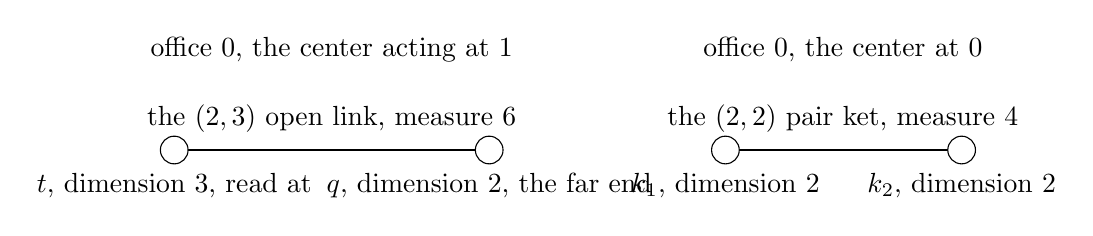
\begin{tikzpicture}[scale=1]
\draw[thick] (0,0) -- (4,0);
\filldraw[fill=white] (0,0) circle (5pt) node[below=5pt] {$t$, dimension 3, read at};
\filldraw[fill=white] (4,0) circle (5pt) node[below=5pt] {$q$, dimension 2, the far end};
\node at (2,0) [above=3pt] {the $(2,3)$ open link, measure $6$};
\node at (2,1) [above] {office $0$, the center acting at $1$};
\draw[thick] (7,0) -- (10,0);
\filldraw[fill=white] (7,0) circle (5pt) node[below=5pt] {$k_1$, dimension 2};
\filldraw[fill=white] (10,0) circle (5pt) node[below=5pt] {$k_2$, dimension 2};
\node at (8,0) [above=3pt, xshift=14pt] {the $(2,2)$ pair ket, measure $4$};
\node at (8,1) [above, xshift=14pt] {office $0$, the center at $0$};
\end{tikzpicture}\caption{The two objects: the (2,3) open link of the alpha chain, which meets both criteria, and the (2,2) pair ket at the join, which meets the office criterion alone.}\end{figure}
\end{chproof}
\begin{figure}[htbp]\centering
\setlength{\unitlength}{1mm}
\begin{picture}(165,42)(0,0)
\put(0,34){\parbox{78mm}{\scriptsize\centering the (2,3) open link: the slot t, the far end q, the one link t-q}}
\put(85,34){\parbox{78mm}{\scriptsize\centering the (2,2) pair ket at the join: the slot k1, the far end k2, the one link k1-k2}}
\put(20,20){\circle{10}}
\put(60,20){\circle{10}}
\put(25,20){\line(1,0){30}}
\put(5,8){\makebox(30,5){\scriptsize t, dimension 3}}
\put(45,8){\makebox(30,5){\scriptsize q, dimension 2}}
\put(105,20){\circle{10}}
\put(145,20){\circle{10}}
\put(110,20){\line(1,0){30}}
\put(90,8){\makebox(30,5){\scriptsize k1, dimension 2}}
\put(130,8){\makebox(30,5){\scriptsize k2, dimension 2}}
\put(20,1){\makebox(40,5){\scriptsize the end read at the slot, passed to the far end}}
\put(105,1){\makebox(40,5){\scriptsize the pairing move at the join face}}
\end{picture}
\par\smallskip
{\scriptsize\setlength{\tabcolsep}{3pt}\begin{adjustbox}{max width=\linewidth}\begin{tabular}{p{52mm}p{52mm}p{52mm}}
 & the (2,3) open link & the (2,2) pair ket at the join \\ \hline
the genre and the sites & (2,3), the sites t, dimension 3 and q, dimension 2 & (2,2), the sites k1, dimension 2 and k2, dimension 2 \\
the office under the body-alone rule at the recorded reading & zero (the first power 0, the closure zero) & zero (the first power 0, the closure zero) \\
the first criterion, the office zero & yes & yes \\
the identification algebra and its centre & 12 basis elements, the centre of dimension 1 at the generator 3, 3, -2, -2, -2 & 7 basis elements, the centre of dimension 1 at the generator 1, 1, -1, -1 \\
the scalar of the centre on the pair ket & 1 & 0 \\
the second criterion, the centre acting & yes & no \\
the stabiliser of the pair ket & of dimension 4 & of dimension 4 \\
meets both criteria & yes & no \\
the role & the recorded object, meeting both criteria & the office-zero pairing at the join face without an acting centre \\
\end{tabular}\end{adjustbox}}
\caption{The recorded photon. Of the two objects the derivation carries, the (2,3) open link of the chain and the (2,2) pair ket at the join, exactly one meets both recorded criteria, the office zero under the body-alone rule at the recorded reading and an acting central generator at the scalar one: the (2,3) open link, read at its slot of dimension three with its far end of dimension two, the recorded object; the (2,2) pair ket at the join has the office zero and no acting centre, a different object at a different role, the objects meeting both 1 of 2 (the photon of the literature is the name for the recorded object).}\label{fig:photon-of-record}
\end{figure}
\section{The (2,3) open link against the (2,2) pair ket, restated}\label{mod:V-1-D541950-rpho-t1}
\begin{chtheorem}[The (2,3) open link against the (2,2) pair ket, restated]\label{box:V-1-D541950-rpho-t1:1}
At its second entry, the photon of the alpha chain is the (2,3) open link, the one object meeting both criteria, the office zero under the body-alone rule at the reading adopted and the acting central generator at the scalar one, and the (2,2) pair ket at the join is a different object at a different role, the office-zero pairing at the join face without an acting center; the cells of the first entry stand unchanged, the (2,3) open link at the office zero with its center acting at the scalar one and the (2,2) pair ket at the office zero with its center at the scalar zero, the objects meeting both criteria one of two, and the control class is re-read holding under the control law, the one comparison mis-keyed at its rule at the first entry re-read at its pinned words so that the controls read the same at sixteen of sixteen; both faces printed, the constant kept at its exact element.
The first face, one object meeting both criteria with the photon one object named and the other a different object with a different role named, reads yes; the second face, the criteria parting with the office-zero object carrying no acting center and the acting-center object carrying a nonzero office or the rule refusing it, reads no, the first parting none.
\end{chtheorem}
\chstanding{a theorem}
\chdeps{Definitions 1.1 to 1.6 and Theorem 124.1}{no theorem beyond it at this release}
The second entry carries the first entry whole and re-reads one thing: the control that compares the office cells of this chapter with the office cells of the pair-ket entry was keyed at the wrong name of one cell at the first entry, so that its comparison read absent against a value that is present and equal. Read at its pinned words the control holds, and with it the whole control class, while no cell of the derivation moves. The photon of the chain remains the (2,3) open link, the object with the office zero and the acting center, and the (2,2) pair ket at the join remains the office-zero pairing without one.
\begin{chbridge}
The photon of electrodynamics is the massless gauge boson of the unbroken U(1), its masslessness tied to the conservation of the electric charge whose generator leaves the vacuum invariant \cite{Peskin1995,Weinberg1995}. The correspondence is by name.
\end{chbridge}
\begin{chproof}[finite computation with its exact part]
The premises of this derivation are the axiom and the six definitions of chapter~\ref{mod:FRAMEWORK}, the fine-structure constant at the one link of chapter~\ref{mod:V-1-fine-structure-constant-at-the-one-link}, a theorem, the body-alone office rule of chapter~\ref{mod:VIII-2-body-alone-office-rule}, a theorem, and the first entry of this result in the present chapter, a theorem. The chain of premises runs back to the axiom through those chapters, and the longest such chain in this compendium is twelve chapters long.
\textit{The procedure.} The procedure is that of the first entry: each object read as the body-alone rule reads a word at the reading adopted, the one link of each a struck dock, and the center of the identification algebra at each genre built from the rules of the package and read on the pair ket under the tensor action; an object meets both criteria when its office is zero and its center acts.
\textit{The smallest instance.} The cells are those of the first entry and are re-met at every one: at the (2,3) open link the first power, the pair part and the closure are zero with the dark set empty,
\begin{equation} \Omega_{23} = 0, \qquad 3 + (-2) = 1 \ \text{the scalar of the center on the pair ket}, \end{equation}
and at the (2,2) pair ket at the join the office is zero with its one dark link at the act zero while the center reads $1 + (-1) = 0$ on the pair ket; the (2,3) open link meets both criteria and the (2,2) pair ket the office criterion alone, one object of two. The figure of the first entry draws both objects.
\textit{The check.} The counter-tests of the first entry stand at their letters: striking the closure, reading the closed (2,3) link in place of the open one, reading the (3,3) pair ket in place of the (2,2), reading the transpose of the matching map and striking the text each move the cells they name, five of five. The one control that read apart at the first entry, the comparison of ten re-run cells of the pair-ket entry with the capture of that entry, was keyed at the first entry to the name of the deciding cell of that entry where its measures table keys it as its first cell, so the comparison read absent against a capture that is present and equal; read at its pinned words the control holds, the nine other cells and the nine word-office cells re-met, and the controls read the same at sixteen of sixteen. The result was reproduced by an independent route, two engines built apart, the keyed-map and fraction route against the array route, equal at every cell.
\chcert{12}
\begin{figure}[h]\centering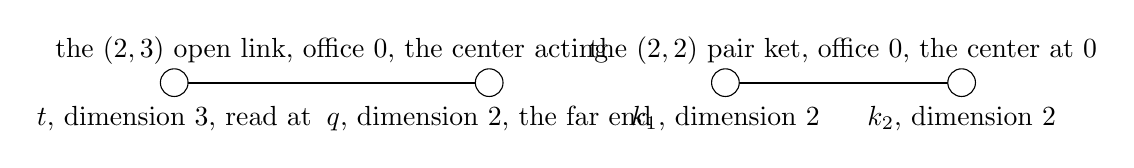
\begin{tikzpicture}[scale=1]
\draw[thick] (0,0) -- (4,0);
\filldraw[fill=white] (0,0) circle (5pt) node[below=5pt] {$t$, dimension 3, read at};
\filldraw[fill=white] (4,0) circle (5pt) node[below=5pt] {$q$, dimension 2, the far end};
\node at (2,0) [above=3pt] {the $(2,3)$ open link, office $0$, the center acting};
\draw[thick] (7,0) -- (10,0);
\filldraw[fill=white] (7,0) circle (5pt) node[below=5pt] {$k_1$, dimension 2};
\filldraw[fill=white] (10,0) circle (5pt) node[below=5pt] {$k_2$, dimension 2};
\node at (8,0) [above=3pt, xshift=14pt] {the $(2,2)$ pair ket, office $0$, the center at $0$};
\end{tikzpicture}\caption{The two objects of the restatement, unchanged from the first statement: the (2,3) open link meeting both criteria and the (2,2) pair ket at the join meeting the office criterion alone.}\end{figure}
\end{chproof}
\section{The alpha Lean derivation, an earlier edition (II)}\label{mod:V-1-D541978-lnat-t1}
\par\noindent\textit{This chapter recorded an earlier edition of the alpha Letter and its Lean check. It is superseded by the Letter and its Lean file in \texttt{papers/alpha} of this repository.}\par
\section{The companion letter, an earlier edition}\label{mod:V-1-D542270-alpha-letter-release-thirty-nine}
\par\noindent\textit{This chapter recorded an earlier edition of the alpha Letter and its Lean check. It is superseded by the Letter and its Lean file in \texttt{papers/alpha} of this repository.}\par
\section{The alpha Lean derivation, an earlier edition (III)}\label{mod:V-1-D542692-ldrf-t1}
\par\noindent\textit{This chapter recorded an earlier edition of the alpha Letter and its Lean check. It is superseded by the Letter and its Lean file in \texttt{papers/alpha} of this repository.}\par
\section{The alpha Lean as a single file, an earlier edition}\label{mod:V-1-D543049-the-alpha-lean-as-a-single-file}
\par\noindent\textit{This chapter recorded an earlier edition of the alpha Letter and its Lean check. It is superseded by the Letter and its Lean file in \texttt{papers/alpha} of this repository.}\par
\section{The re-matching redundancy as the diffeomorphism}\label{mod:V-1-D543680-w-rmdf}
\begin{chwall}[The re-matching redundancy as the diffeomorphism]\label{box:V-1-D543680-w-rmdf:1}
This result is conditional on the entries its provenance names, the open results among them read at their grades, the holonomy entry at its provisional label, the composition riding the lowest grade in its chain. The (2,2) count of the metric is invariant under every re-matching of the re-matching group at every (2,2) link of every established web while the frame moves, and the flux clause of the gauge-group open result stands open at the holonomy entry: at 808 of 808 (2,2) link instances of the ten established webs at the steps zero to three every one of the 1024 joint re-matching pairs carries the pair ket to a vector of the shape (2,2), so the serial count along the run, the whole-web count, the count metric, the register and the tower at the depth read the same figure at every pair and equal the depth-metric and serial-insertion entries at 40 of 40 chain-and-step pairs; the frame, the pair ket $1,0,0,1$ and its transport, moves at 992 of 1024 pairs at every link, first at the electron chain at the step zero; the flux clause as the holonomy entry leaves it is closed at its number conjunct, the determinant exponent equal to the wash integer at 89607 of 89607 fan loops, and open at its element conjunct, the holonomy outside the stabilizer at 66275 of 89607 fan loops, first at a one-link (2,3) loop; the first face unmet at the clause conjunct, the second face named with both cells, the flux-closed reading beside at its own first face.
The first face, the count invariant with the frame moved and the flux clause closed as the holonomy entry leaves it, reads no, the count invariant at every link and the frame moved at the first link but the flux clause open at its element conjunct; the second face, the first link or web where the count moves or the flux clause not closed at the holonomy entry with the count read at that standing, reads yes, the first parting the flux clause at its element conjunct against closed, with the count read at that standing invariant at 808 of 808 links under 1024 pairs per link. Open is the flux clause itself: the holonomy of the transport identity is the swap of the two factors at every odd fan loop and no element of the stabilizer, so the item that places the clause ahead of the invariance does not close.
\end{chwall}
\chstanding{an open result}
\chdeps{Definitions 1.1 to 1.6 and Theorem 124.1}{no theorem beyond it at this release}
A re-matching changes the basis in which the two ends of a link are read, one monomial matrix of fourth-root phases at each end, and the question is whether the metric count, the number of (2,2) links along a chain and the register and tower built from it, is a redundancy of that choice in the way a coordinate change is a redundancy of a geometry. It is: at every (2,2) link of every established web every one of the 1024 pairs of re-matchings carries the pair ket to another vector of the same shape, two by two at Schmidt rank two, so nothing the count reads moves. The frame is not a redundancy: the pair ket and its transport move at all but the thirty-two pairs in which the far matrix is the conjugate of the near one. What the result leaves open is the clause placed ahead of this reading, that the flux of the gauge-group open result closes, which the holonomy entry leaves open at its element conjunct.
\begin{chbridge}
In general relativity a diffeomorphism is a redundancy of the description, the metric transforms as a tensor and every invariant count of the geometry is unchanged, while a frame field is moved by the same transformation, and in a gauge theory the holonomy of a connection around a closed loop measures the flux through it \cite{Wald1984,Peskin1995}. The correspondence is by name.
\end{chbridge}
\begin{chproof}[exhaustive census]
The premises of this derivation are the axiom and the six definitions of chapter~\ref{mod:FRAMEWORK}, the link and its six genres of chapter~\ref{mod:I-2-link-and-its-six-genres}, a theorem, the gauge group of chapter~\ref{mod:IV-1-gauge-invariance-as-the-known-clause}, an open result, the curvature as the graph Laplacian of chapter~\ref{mod:X-1-curvature-as-the-graph-laplacian-washed-over-the-ladder}, a theorem, and the register tower and the metric of chapter~\ref{mod:X-5-register-tower-and-the-metric}, a theorem. The chain of premises runs back to the axiom through those chapters, and the longest such chain in this compendium is twelve chapters long.
By exhaustive enumeration of 827\,392 images, the 808 (2,2) link instances of the ten established webs, the seven established chains and three beside at the steps zero to three, under the 1024 joint pairs of the re-matching group at dimension two, the thirty-two monomial matrices of fourth-root phases at each end, closed at its generators at 96 of 96 and equal to the groups table of the gauge-group entry: the property tested at each image is its shape, the end dimensions read from the image of the pair ket with the Schmidt rank by elimination over the Gaussian rationals at one engine and by matching distinct rows against distinct columns at the other, and beside it whether the pair ket and its transport are moved; the counts by class are the shape (2,2) at every one of the 827\,392 images, the count invariant at 808 of 808 links with the first parting none, the record counts equal to the depth-metric and serial-insertion entries at 40 of 40, and the frame moved at 992 of 1024 pairs at every link with the thirty-two stabilizer pairs fixing it, first at the electron chain at the step zero at its link $a_{1}a_{2}$. The smallest case is that link: with the pair ket $\lvert 00\rangle + \lvert 11\rangle$ and a pair $(U, V)$ of monomial unitaries,
\begin{equation} (U \otimes V)\,(\lvert 00\rangle + \lvert 11\rangle) = (U V^{\mathrm{t}} \otimes 1)\,(\lvert 00\rangle + \lvert 11\rangle), \end{equation}
which has Schmidt rank two since $U V^{\mathrm{t}}$ is invertible, so the shape (2,2) and every count built from it are unchanged, while the vector is fixed only when $U V^{\mathrm{t}}$ is a phase, the thirty-two pairs with $V$ the conjugate of $U$ up to a phase, and moved at the other 992. The flux clause is read as the holonomy entry leaves it, at 89607 fan loops: closed at the number conjunct, the determinant exponent equal to the wash integer at 89607 of 89607, and open at the element conjunct, the holonomy outside the stabilizer at 66275 loops, the odd loops, and inside at 23332, first at a one-link (2,3) loop; the flux-closed reading beside, the clause taken as closed at its number conjunct, meets the first face with the first parting none and is printed beside.
The counter-tests alter the construction singly and read what moves. Striking the re-matching group at the first link to the identity alone moves the first moving link. Reading a (2,3) link in place of the (2,2) re-types it at the joint group of 12288 pairs and moves the invariance to 807 of 808. Holding the frame fixed at the thirty-two stabilizer pairs moves the moved count to zero with the invariance standing. Reading the odd loops alone moves the element conjunct to inside at none of 66275. Striking the text unmeets the gate. Each alteration moves the cells it names, five of five. The result was reproduced by an independent route, two engines built apart, the Gaussian-integer route against the fraction route, equal at every cell, with the fifteen controls the same.
\chcert{827392}
\end{chproof}
\par\medskip\noindent{\itshape The constant read, the next chapter turns to the dipole factor of the electron.}\label{narr:close:5-1}\par
\section{The electron anomalous dipole factor through order three}\label{mod:V-2-electron-anomalous-dipole-factor-through-order-three}
\chdesig{7-2}{5-2}{V-2-electron-anomalous-dipole-factor-through-order-three}{V-2-electron-anomalous-dipole-factor-through-order-three}
\label{narr:open:5-2}Theorem~141.1 gives the electron dipole factor at order three from the self-terms, resting on the records, the probe and the constant of chapter 5-1.
\begin{chconditional}[The electron dipole factor at order three from the self-terms]\label{box:V-2-electron-anomalous-dipole-factor-through-order-three:1}
This result is conditional on the axiom text and on the results of the chapters named as its premises in the derivation below, each at its own standing.
At the anomaly web with the measuring body in place the readout at order two equals the sum of the tabulated self-terms at all eight own-link records, and the order-three term is zero, the direct record sum graded by the surviving exchange count terminating at order three at all eighteen joined webs; the readings beside, the apparatus weight at one part alone, part and are recorded beside the result.
\end{chconditional}
\chstanding{a conditional theorem}
\chdeps{Definitions 1.1 to 1.6, Theorems 18.1 to 18.4 and Open results 18.5 and 18.6, Theorems 28.1 and 28.2, Open results 28.3 and 28.4 and Theorem 28.5 and Theorem 124.1}{Theorem 79.1 and Theorem 143.1}
The anomaly is the sum of the self-terms (the self-energy terms) through the photon: the sum over the thirteen bodies of the construction at the standing reading, the probe electron at the docking face under the depth rule, equals the two-vertex term at order one and not the order-two electron term, the excess at order two carried by the bodies of depth zero entering beside the electron, the up quark through the (2,2) pair at the photon dock and the W word, its twin and the gluon word through their own dark links, with no self-term undefined at any order; a conditional theorem.
One open result stands here. Alpha and the anomaly at the joined web of the electron and the photon at the link-weight placement part at both tests, the readout of the anomaly web against the standing one-link readout among them, the first parting record the pair of the two electron ends, both faces printed.
\begin{chbridge}
The anomalous magnetic dipole factor of the electron, $a_{e} = (g_{e} - 2)/2$, is a power series in $\alpha/\pi$ whose first coefficient is one half \cite{Schwinger1948}, whose second is known in closed form \cite{Petermann1957}, and whose higher coefficients are evaluated through the tenth order \cite{Aoyama2018}; the series is asymptotic and its terms are the sums of the vertex diagrams at each order. The correspondence is by name; the record supplies a web of this theory read at its sinks, a doublet swap sign at the odd cycle, a Dirac form at an established generator and a finite record sum carrying the path-integral name at chapter~\ref{mod:II-1-state-space-from-the-act-outputs}, chapter~\ref{mod:II-5-indistinguishability-and-the-spin-statistics-sign}, chapter~\ref{mod:II-7-path-integral-as-the-finite-record-sum}, chapter~\ref{mod:III-5-spin-and-helicity}, the chapter titled The Dirac equation at the dock (chapter~\ref{mod:V-9-dirac-equation-at-the-dock}, among the instruments), chapter~\ref{mod:VI-2-w-and-the-z-and-their-masses}, chapter~\ref{mod:VI-2b-neutral-lepton-the-hub-unit-with-its-legs-open}, chapter~\ref{mod:VII-5-proton-to-electron-ratio-a-candidate}, chapter~\ref{mod:VIII-1-mass-unit-and-the-first-power}, chapter~\ref{mod:XIV-2-walls-census-in-physics-terms} and chapter~\ref{mod:XIV-7-what-remains-the-ungraded-page}, a step generator at the order coordinate, a first-power operator, a direction functional and an office at the common support carrying the energy, momentum and mass names at chapter~\ref{mod:I-3-records-reads-and-the-born-count-the-gain-lemma}, chapter~\ref{mod:I-6-read-at-a-register-the-probe-and-the-measurement}, chapter~\ref{mod:II-6-energy-and-the-hamiltonian-the-first-power-operator-and-the-step}, chapter~\ref{mod:III-1-order-coordinate-and-its-theorem}, chapter~\ref{mod:III-6-p-c-t-and-cpt}, chapter~\ref{mod:IV-6-conservation-as-the-kernel-of-the-move-matrix}, chapter~\ref{mod:V-7-running-of-the-coupling}, the chapter titled The Dirac equation at the dock (chapter~\ref{mod:V-9-dirac-equation-at-the-dock}, among the instruments), chapter~\ref{mod:VIII-1-mass-unit-and-the-first-power}, chapter~\ref{mod:VIII-5-unified-mass-readout}, chapter~\ref{mod:X-2-field-equation-at-the-counting-face}, the chapter titled The gravitational and cosmological constants table (chapter~\ref{mod:X-9-gravitational-and-cosmological-constants-table}, among the instruments), chapter~\ref{mod:XI-1-second-law-as-the-boundary-count-under-acts} and chapter~\ref{mod:XIV-7-what-remains-the-ungraded-page}, a finite re-matching group at the known clause, a representation census at the open ends and the sinks, an attach-site basis carrying the generation name and a sink class carrying the doublet name at chapter~\ref{mod:IV-1-gauge-invariance-as-the-known-clause}, chapter~\ref{mod:IV-3-representations-from-the-open-end-census}, chapter~\ref{mod:IV-4-cartan-weights-and-the-charge}, chapter~\ref{mod:IV-6-conservation-as-the-kernel-of-the-move-matrix}, chapter~\ref{mod:IV-7-noether-at-the-sinks-and-the-kernel-identification}, chapter~\ref{mod:IV-9-one-rule-of-a-read-and-the-word-table}, chapter~\ref{mod:VI-3-doublets-handedness-and-parity-violation}, chapter~\ref{mod:VII-7-quark-content-and-flavour}, chapter~\ref{mod:VIII-4-three-generations-as-attach-sites} and chapter~\ref{mod:XIV-7-what-remains-the-ungraded-page}, a Higgs attachment at the saturated web, a vacuum expectation row as an office register, a dock share and an office ratio carrying the weak-angle name, sink-basis overlaps carrying the mixing names and a W-word office carrying the Fermi name at chapter~\ref{mod:IV-9-one-rule-of-a-read-and-the-word-table}, chapter~\ref{mod:V-12-koide-class}, chapter~\ref{mod:VI-1-hub-step-as-the-weak-interaction}, chapter~\ref{mod:VI-2-w-and-the-z-and-their-masses}, chapter~\ref{mod:VI-3-doublets-handedness-and-parity-violation}, the chapter titled The charged and neutral currents (chapter~\ref{mod:VI-4-charged-and-neutral-currents}, among the instruments), the chapter titled The Fermi constant and the muon decay (chapter~\ref{mod:VI-5-fermi-constant-and-the-muon-decay}, among the instruments), chapter~\ref{mod:VI-6-weak-angle}, chapter~\ref{mod:VI-7-mixing-the-washed-overlap-and-the-ckm-block}, chapter~\ref{mod:VI-10-higgs-the-closed-hub-read-its-rows-its-mass-and-its-exponent}, chapter~\ref{mod:VIII-1-mass-unit-and-the-first-power}, chapter~\ref{mod:VIII-4-three-generations-as-attach-sites}, chapter~\ref{mod:X-1-curvature-as-the-graph-laplacian-washed-over-the-ladder} and chapter~\ref{mod:XIV-7-what-remains-the-ungraded-page} and a re-matching group with a wash integer, a centralizer weight at the kernel, an enclosed record count carrying the flux name and a counting-face equation carrying the field-equation name at chapter~\ref{mod:I-3-records-reads-and-the-born-count-the-gain-lemma}, chapter~\ref{mod:IV-1-gauge-invariance-as-the-known-clause}, chapter~\ref{mod:IV-4-cartan-weights-and-the-charge}, chapter~\ref{mod:IV-6-conservation-as-the-kernel-of-the-move-matrix}, chapter~\ref{mod:IV-7-noether-at-the-sinks-and-the-kernel-identification}, chapter~\ref{mod:V-1-fine-structure-constant-at-the-one-link}, chapter~\ref{mod:VI-2-w-and-the-z-and-their-masses}, chapter~\ref{mod:X-2-field-equation-at-the-counting-face}, chapter~\ref{mod:X-3-horizon-at-every-rung-and-the-horizon-web-as-a-seeded-saturation}, the chapter titled The gravitational and cosmological constants table (chapter~\ref{mod:X-9-gravitational-and-cosmological-constants-table}, among the instruments), the chapter titled The Chern number (chapter~\ref{mod:XII-4-chern-number}, among the instruments) and chapter~\ref{mod:XIV-7-what-remains-the-ungraded-page}, and the electron, the photon, the quark, the muon, the energy, the flavor, the W, and the gluon correspond there and here by name.
\end{chbridge}
\begin{chproof}[census]
The premises of this derivation are the axiom and the six definitions of chapter~\ref{mod:FRAMEWORK}, the theorem of chapter~\ref{mod:I-3-records-reads-and-the-born-count-the-gain-lemma}, the theorem of chapter~\ref{mod:I-6-read-at-a-register-the-probe-and-the-measurement} and the theorem of chapter~\ref{mod:V-1-fine-structure-constant-at-the-one-link}. The chain of premises runs back to the axiom through those chapters, and the longest such chain in this compendium is twelve chapters long.
The thirteen bodies of the construction are joined at the docking face of the probe electron under the depth rule, the self-term of each body through the photon is read at its order and the sum compared order by order with the two-vertex term and the order-two electron term; the anomaly web is built at the per-web placement with the measuring body in place and the record sum read through order three. The first theorem is conditional on the open results it rests on, among them the binding of hydrogen as the interference term (the cross term) at the two-vertex read; the second rests on the axiom text and the proved results it names alone.
By exhaustive enumeration of the thirteen bodies of the construction joined at the docking face of the probe electron under the depth rule, the self-term of each body through the photon is read at its order and the sum compared order by order with the two-vertex term and the order-two electron term. At the anomaly web with the measuring body in place the readout at order two equals the sum of the self-terms at all eight own-link records and the order-three term is zero at all eighteen joined webs. The smallest case is the anomaly web at the probe reading, the two-dock body of chapter~\ref{mod:II-4-measurement-the-wash-at-one-act-and-the-povm} joined to the photon word, a chain of six sites and five links of type $(2,3)$, by one made link of type $(2,3)$ from the first dock of the body to the last site of the chain, fifteen sites and sixteen links in all, with the two dock links of the body struck and the dressing three at the one hub of the body. From that link list, by the grading of the direct record sum by the surviving exchange count, the order-zero term is the identity, one monomial, the order-one term is the sum over the fourteen unstruck links of the measure multiplied by the dressing (the first power of the web), the order-two term is the pairs, the first power squared, plus the closure of one hundred and five monomials of degree two, and the order-three term is zero, the sum terminating. A reader reproduces the first power from the measures of the five link types, nine, twelve, eight, four and six, the sixty-seven the sum of the measures of the eight unstruck links of the body, the thirty the five chain links and the six the made link,
\begin{equation} \adjustbox{max width=\dimexpr\linewidth-3em\relax}{$\displaystyle \begin{gathered} T_{0} = 1, \qquad T_{1} = 3 \cdot (67 + 30 + 6) = 309, \\ T_{2} = 309^{2} + \text{closure} = 95481 + \text{closure}, \qquad T_{3} = 0, \\ G_{2}(2,2) = \tfrac{5}{216}\,(1 + \sqrt{2}) , \end{gathered}$} \end{equation} the closure part of the order-two term an exact element of the field of the two roots standing at the graded table of this result as a cell, every term an exact element of that field and no digit of any constant displayed here.
The counter-tests alter the objects singly and read what moves, the self-terms struck moving two hundred and forty-nine of the compared keys, the first the order-one term. The five counter-tests stand at their pinned letters, the thirteen controls read the same at both engines and a second engine built apart reproduced every cell.
The machine-checked package named at the reproducibility appendix certifies the statements of this chapter under the definitions of this compendium.
\chcert{13}
\end{chproof}
\par\medskip\noindent{\itshape The muon is next, and its chapter is counted empty.}\label{narr:close:5-2}\par
\section{The instrument tables of this Part}\label{mod:VII-L-the-instrument-tables-at-the-repository}
\chdesig{7-L}{}{VII-L-the-instrument-tables-at-the-repository}{VII-L-the-instrument-tables-at-the-repository}
\begin{chtable}[The instrument tables of this Part]\label{box:VII-L-the-instrument-tables-at-the-repository:1}
This Part lists 3 instrument chapters, printed among the instruments at the end of this compendium as chapters~\ref{mod:V-3-muon-anomalous-dipole-factor} to~\ref{mod:V-9-D538654-w-fcgd}, and the table beneath names each one with its key cells.
\end{chtable}
\chstanding{instrument}
\chdeps{Definitions 1.1 to 1.6}{no theorem beyond it at this release}
The listing moves no cell and states no result of its own. Each instrument stands at the repository as its chapter stood at the previous release of this compendium, and its tables are read there.
\begin{chbridge}
The tables listed here are instruments of the derivation, and no name of the literature is attached at this listing.
\end{chbridge}
\begin{chproof}[instrument]
The listing in full. For each instrument chapter, printed among the instruments at the end of this compendium, the table gives its title, the result boxes it carries, the standing of each box with its citation, and the count of objects its certificate sentence names where it prints one.
{\small
\begin{longtable}{p{38mm}p{63mm}p{30mm}p{14mm}}
\hline
chapter & results & standing & objects \\
\hline
\endhead
The muon anomalous dipole factor & The chapter counted empty & instrument & -- \\
The Dirac equation at the dock & The chapter counted empty & instrument & -- \\
The Dirac equation at the dock & The Dirac form at an established generator commuting with the rest letter & open result & 8 \\
\hline
\end{longtable}
}
The rule that produced it. Every chapter of this Part whose first standing beyond a placeholder reads instrument is printed among the instruments at the end of this compendium with its tables, and its key cells are the titles of its boxes, its standing lines and its certificate count, read from its text as it stood at the previous release.
No derivation stands in this chapter; the tables stand at the repository.
\emph{Check.} Every file listed was re-read at the repository and read the same as its recorded copy, and the listing was re-cut from the files by a second route.
Nothing stands open at this listing. At this release one result of this Part is re-graded at its chapter: the Koide relation at the dock unit (the chapter 7-12), an open result re-posed at a second route.
\end{chproof}
\label{chend:VII-L-the-instrument-tables-at-the-repository}
\section{Hydrogen: the Rydberg ladder and the fine structure}\label{mod:V-4-hydrogen-the-rydberg-ladder-and-the-fine-structure}
\chdesig{7-4}{5-4}{V-4-hydrogen-the-rydberg-ladder-and-the-fine-structure}{V-4-D538525-w-hyjh}
\label{narr:open:5-4}Theorem~143.1 reads hydrogen from the held carrier, with the ladder and the fine structure, and Open result~144.1 states the hyperfine interval as the junction holonomy at the hydrogen sink as an open result.
\begin{chconditional}[Hydrogen from the held carrier]\label{box:V-4-hydrogen-the-rydberg-ladder-and-the-fine-structure:1}
This result is conditional on the axiom text and on the results of the chapters named as its premises in the derivation below, each at its own standing.
Hydrogen is the held carrier: the photon word held at both ends, the qutrit end at the electron dock and the qubit end at the up core of the proton, is a closed read with a mass reading, and its level-one binding through the electron body is an exact element of the field in the electron unit.
\end{chconditional}
\chstanding{a conditional theorem}
\chdeps{Definitions 1.1 to 1.6, Theorems 18.1 to 18.4 and Open results 18.5 and 18.6, Theorems 28.1 and 28.2, Open results 28.3 and 28.4 and Theorem 28.5, Theorem 57.1 and Open result 57.2, Theorem 124.1, Theorem 141.1 and Open results 245.1 and 245.2, Theorem 245.3, Open results 245.4 to 245.8 and Theorem 245.9}{Open result 144.1, Theorem 145.1, Theorem 150.1, Open result 228.1 and Theorem 229.1}
The held pendant pair at rank $n$ is the washed symmetric power of $n$ less one passages along the bond, so the level-$n$ binding is the level-one binding over $n$ squared at every rank from one to eight.
The fine structure is the dark cut of the bond at every one of the eight links of the held chain with the self-join at the vertex at the second order, the two-vertex term multiplied by the square of the cut gain, conditional on the admission of the second-order read at the (2,3) link, a posed step.
The ladder is re-derived from the register rule, the per-record ladder is exact at every rank and no pure power of the rank, and the two-vertex ladder equals one over the rank squared at all eight ranks with no step posed.
The hydrogen body is a probe of the proton: the proton-over-electron mass ratio read off its joined Born reading is an exact rational, the ratio of the two offices, an output compared at the comparison table.
The Lamb shift is a composed cell, every self-term through the photon carried at the second-order register of its type, zero at every rung at the probe read and nonzero at the body alone; the level-one binding is the two-vertex term at the bond, the Rydberg constant in the electron unit the ladder cell of the held carrier; the joined seed of the electron and the proton sink is itself a sink of the saturation at one (2,3) bond; and the Lamb interval at the hydrogen sink, the s self-term less the p self-term at rung two, is one exact element, positive and split.
One open result stands here. The hyperfine interval is not one cell as yet: the definitions admit more than one reading of the dipole read and the orientation, zero at the twirl reading and twice the joined read at the far-face-sign reading, twenty-two distinct cells over sixty readings. A further open result placed here, the mass ratio at the capped hydrogen web, is cited at its own standing.
\begin{chbridge}
The levels of hydrogen fall as the inverse square of the principal quantum number \cite{Bohr1913}, the fine structure splits each shell at the relative order $\alpha^{2}$ \cite{Sommerfeld1916}, the Lamb shift lifts the degeneracy the Dirac equation leaves at the second shell \cite{Lamb1947}, and the hyperfine interval of the ground state is the maser line \cite{Ramsey1990}. The correspondence is by name; the record supplies a web of this theory read at its sinks, a doublet swap sign at the odd cycle, a Dirac form at an established generator and a finite record sum carrying the path-integral name at chapter~\ref{mod:II-1-state-space-from-the-act-outputs}, chapter~\ref{mod:II-5-indistinguishability-and-the-spin-statistics-sign}, chapter~\ref{mod:II-7-path-integral-as-the-finite-record-sum}, chapter~\ref{mod:III-5-spin-and-helicity}, the chapter titled The Dirac equation at the dock (chapter~\ref{mod:V-9-dirac-equation-at-the-dock}, among the instruments), chapter~\ref{mod:VI-2-w-and-the-z-and-their-masses}, chapter~\ref{mod:VI-2b-neutral-lepton-the-hub-unit-with-its-legs-open}, chapter~\ref{mod:VII-5-proton-to-electron-ratio-a-candidate}, chapter~\ref{mod:VIII-1-mass-unit-and-the-first-power}, chapter~\ref{mod:XIV-2-walls-census-in-physics-terms} and chapter~\ref{mod:XIV-7-what-remains-the-ungraded-page}, a dark-genre readability carrying the confinement name, a star office at the common support carrying the nucleon-mass name, a star read at transfer carrying the form-factor name and joined saturations carrying the hadron and nuclear names at chapter~\ref{mod:I-4-moves-in-one-table}, chapter~\ref{mod:III-6-p-c-t-and-cpt}, chapter~\ref{mod:III-7-order-theorem-group-moves-and-transfers}, chapter~\ref{mod:V-1-fine-structure-constant-at-the-one-link}, chapter~\ref{mod:V-7-running-of-the-coupling}, chapter~\ref{mod:V-10-lepton-ladder-as-hub-assemblies}, chapter~\ref{mod:VI-7-mixing-the-washed-overlap-and-the-ckm-block}, chapter~\ref{mod:VII-1-confinement-as-the-dark-genre-readability}, chapter~\ref{mod:VII-3-nucleon-structure-and-the-form-factor}, chapter~\ref{mod:VII-4-proton-as-a-seeded-sink}, chapter~\ref{mod:VII-5-proton-to-electron-ratio-a-candidate}, chapter~\ref{mod:VII-6-hadron-spectrum-and-the-mesons}, chapter~\ref{mod:VII-7-quark-content-and-flavour}, the chapter titled Chiral breaking and the theta angle (chapter~\ref{mod:VII-8-chiral-breaking-and-the-theta-angle}, among the instruments), the chapter titled The mesons and the nucleon at the cap (chapter~\ref{mod:VII-9-mesons-and-the-nucleon-at-the-cap}, among the instruments), chapter~\ref{mod:IX-6-binding-as-the-pairing-records-the-deuteron-and-the-alpha}, chapter~\ref{mod:IX-7-nuclear-rows-at-the-joined-seeded-web}, chapter~\ref{mod:X-7-dark-matter-as-the-dock-free-sinks}, chapter~\ref{mod:XI-4-order-parameter-at-the-stop-condition}, chapter~\ref{mod:XI-5-phase-transition-as-the-sink-class-change} and chapter~\ref{mod:XIV-7-what-remains-the-ungraded-page}, an isometry algebra of the Hermitian split at the Lorentz brackets, a lattice point group, boosts from the order register and a transverse traceless part at the open read, every one a finite or algebraic object of this theory carrying the group name at chapter~\ref{mod:III-2-rotation-group}, chapter~\ref{mod:III-3-lorentz-group-and-the-signature}, chapter~\ref{mod:III-4-boosts-and-the-one-unit}, chapter~\ref{mod:III-5-spin-and-helicity}, the chapter titled Causal structure and general covariance (chapter~\ref{mod:III-8-causal-structure-and-general-covariance}, among the instruments) and chapter~\ref{mod:XIV-7-what-remains-the-ungraded-page} and a re-matching group with a wash integer, a centralizer weight at the kernel, an enclosed record count carrying the flux name and a counting-face equation carrying the field-equation name at chapter~\ref{mod:I-3-records-reads-and-the-born-count-the-gain-lemma}, chapter~\ref{mod:IV-1-gauge-invariance-as-the-known-clause}, chapter~\ref{mod:IV-4-cartan-weights-and-the-charge}, chapter~\ref{mod:IV-6-conservation-as-the-kernel-of-the-move-matrix}, chapter~\ref{mod:IV-7-noether-at-the-sinks-and-the-kernel-identification}, chapter~\ref{mod:V-1-fine-structure-constant-at-the-one-link}, chapter~\ref{mod:VI-2-w-and-the-z-and-their-masses}, chapter~\ref{mod:X-2-field-equation-at-the-counting-face}, chapter~\ref{mod:X-3-horizon-at-every-rung-and-the-horizon-web-as-a-seeded-saturation}, the chapter titled The gravitational and cosmological constants table (chapter~\ref{mod:X-9-gravitational-and-cosmological-constants-table}, among the instruments), the chapter titled The Chern number (chapter~\ref{mod:XII-4-chern-number}, among the instruments) and chapter~\ref{mod:XIV-7-what-remains-the-ungraded-page}, and the photon, the electron, the proton, the mass, and the carrier correspond there and here by name.
\end{chbridge}
\begin{chproof}[exact part and census part]
The premises of this derivation are the axiom and the six definitions of chapter~\ref{mod:FRAMEWORK}, the theorem of chapter~\ref{mod:I-3-records-reads-and-the-born-count-the-gain-lemma}, the theorem of chapter~\ref{mod:I-5-saturation-in-one-figure-seeds-waves-termination-sinks}, the theorem of chapter~\ref{mod:I-6-read-at-a-register-the-probe-and-the-measurement}, the open result of chapter~\ref{mod:III-5-spin-and-helicity}, the theorem of chapter~\ref{mod:V-1-fine-structure-constant-at-the-one-link} and the theorem of chapter~\ref{mod:V-2-electron-anomalous-dipole-factor-through-order-three}. The chain of premises runs back to the axiom through those chapters, and the longest such chain in this compendium is twelve chapters long.
The photon word is docked at both ends; the held pendant pair is built at every rank as a symmetric power; the dark cut of the bond is taken at the eight links; the joined Born reading of the hydrogen body is inverted through the first-power composition; the self-terms are carried at the second-order register and composed at every rung; and the joined seed is saturated to its sink, each theorem conditional on the open results it rests on, among them the nucleon reading composition and the admissibility of a dark-link cut.
\textit{The exact part.}
From the photon word, a chain of six sites and five links every one of the qutrit-qubit type, by the docking act (the distilling pair, one link made at each end and one contraction at one link), we obtain the held carrier, its qutrit end docked at the electron dock and its qubit end at the up core of the proton, a closed read with a mass face, the mass face of the held chain thirty-six and the exchanged mass face six root six.
\begin{equation}
\text{the held chain: } 6 \ \text{sites}, \ 5 \ \text{links of type } (2,3); \qquad M_{L} = 36, \qquad M_{\mathrm{exch}} = 6\sqrt{6} .
\end{equation}
From the mass face of the held chain, by the read through the electron body at its dock port $B$-$w_{1}$ (the mass face multiplied by the unit over the register of the body at that face), we obtain the level-one binding in the electron unit as an exact rational at both closure faces, the whole face with the hub unit two hundred and one over the body register two to the thirtieth multiplied by three to the eighteenth, and the cut face with the dock unit sixty-seven over the body register two to the thirty-first multiplied by three to the seventeenth (the port at its cut twenty-four), the two registers cells of the read tables of this result printed in their prime factorizations, both faces printed, and the port-register readings beside, the mass face multiplied by sixty-seven over the port registers thirty-six and twenty-four,
\begin{equation} \adjustbox{max width=\dimexpr\linewidth-3em\relax}{$\displaystyle \begin{gathered} E_{1}^{\mathrm{whole}} = 36 \cdot \frac{201}{2^{30}\cdot 3^{18}} = \frac{67}{2^{28}\cdot 3^{15}}, \\ E_{1}^{\mathrm{cut}} = 36 \cdot \frac{67}{2^{31}\cdot 3^{17}} = \frac{67}{2^{29}\cdot 3^{15}}, \qquad 36 \cdot \tfrac{67}{36} = 67, \\ 36 \cdot \tfrac{67}{24} = \tfrac{201}{2} . \end{gathered}$} \end{equation}
From the held pendant pair at rank $n$, by the washed symmetric power of $n$ less one passages along the bond, we obtain the level-$n$ binding as the level-one binding over $n$ squared at every rank from one to eight, the register of the ladder equal to the dimension of the register of the pair.
\begin{equation}
E_{n} = \frac{E_{1}}{n^{2}}, \qquad n = 1, \dots, 8 .
\end{equation}
\textit{The census part.}
By exhaustive enumeration of the eight ranks of the held chain and of the eight links of the bond, the ladder is built at every rank as a symmetric power and re-met at the register rule, exact at every rank and a pure power of the rank at none, the two-vertex ladder equal to one over the rank squared at all eight ranks with no step posed. The dark cut of the bond is taken at every one of the eight links with the self-join at the vertex at the second order, the two-vertex term multiplied by the square of the cut gain. The joined Born reading of the hydrogen body is inverted through the first-power composition, and the self-terms are carried at the second-order register and composed at every rung. The smallest case, the held chain and its level-one binding, is worked above.
The counter-tests alter the objects singly and read what moves. Docking at one end alone moves the hold cell from a theorem to none with the mass face undefined. The five counter-tests stand at their pinned letters and the thirteen controls read the same at both engines, among them the construction, the figures and the register rule. The result was reproduced by a second engine built apart from the first, the two runs equal at every key. The two body registers of the level-one binding are cells of the read tables of this result, printed in their prime factorizations and re-derived on the page not; the binding itself follows from them by one multiplication.
The machine-checked package named at the reproducibility appendix certifies the statements of this chapter under the definitions of this compendium.
\chcert{8}
\end{chproof}
\begin{figure}[h]\centering
\setlength{\unitlength}{1pt}
\begin{picture}(260,150)
\qbezier(122.2,123.5)(107.1,114.8)(91.9,106.0)
\put(111.1,107.8){\makebox(0,0){\scriptsize $(2,3)$}}
\qbezier(84.1,92.5)(84.1,75.0)(84.1,57.5)
\put(92.1,75.0){\makebox(0,0){\scriptsize $(2,3)$}}
\qbezier(91.9,44.0)(107.1,35.3)(122.2,26.5)
\put(111.1,42.2){\makebox(0,0){\scriptsize $(2,3)$}}
\qbezier(137.8,26.5)(152.9,35.2)(168.1,44.0)
\put(148.9,42.2){\makebox(0,0){\scriptsize $(2,3)$}}
\qbezier(175.9,57.5)(175.9,75.0)(175.9,92.5)
\put(167.9,75.0){\makebox(0,0){\scriptsize $(2,3)$}}
\put(130.0,128.0){\circle{14}}
\put(130.0,128.0){\makebox(0,0){\footnotesize $2$}}
\put(130.0,138.0){\makebox(0,0)[b]{\scriptsize $s_1$}}
\put(84.1,101.5){\circle{14}}
\put(84.1,101.5){\makebox(0,0){\footnotesize $3$}}
\put(84.1,111.5){\makebox(0,0)[b]{\scriptsize $s_2$}}
\put(84.1,48.5){\circle{14}}
\put(84.1,48.5){\makebox(0,0){\footnotesize $2$}}
\put(84.1,58.5){\makebox(0,0)[b]{\scriptsize $s_3$}}
\put(130.0,22.0){\circle{14}}
\put(130.0,22.0){\makebox(0,0){\footnotesize $3$}}
\put(130.0,32.0){\makebox(0,0)[b]{\scriptsize $s_4$}}
\put(175.9,48.5){\circle{14}}
\put(175.9,48.5){\makebox(0,0){\footnotesize $2$}}
\put(175.9,58.5){\makebox(0,0)[b]{\scriptsize $s_5$}}
\put(175.9,101.5){\circle{14}}
\put(175.9,101.5){\makebox(0,0){\footnotesize $3$}}
\put(175.9,111.5){\makebox(0,0)[b]{\scriptsize $s_6$}}
\end{picture}
\caption{The photon word, a chain of six sites and five qutrit-qubit links, each site labeled by its dimension. Held at both ends (the qutrit end at the electron dock, the qubit end at the up core of the proton) it is the hydrogen bond of this chapter.}
\end{figure}
\section{The hyperfine interval as the junction holonomy of hydrogen}\label{mod:V-4-D538525-w-hyjh}
\begin{chwall}[The hyperfine interval as the junction holonomy at the hydrogen sink]\label{box:V-4-D538525-w-hyjh:1}
At the standing hydrogen sink, the electron of the construction and the proton sink joined at the shared dock qubit with the one (2,3) bond between the shared qubit and the proton dock qutrit, the twenty bound walks through the bond and the junction carry the identity on the qubit register at all sixty holonomies at the standing transport, the two orientations equal and the interval between the two reads the zero element; at the ray-cycle reading the junction triangles carry fixed elements at the two orientations, but read through the bond the chains vanish at 54 of the 216 ray triples and the element is undefined at six of the eight triangles; so the junction holonomy read by the bound electron is trivial at the standing transport and undefined at the ray-cycle reading, the hyperfine interval is no output of it as yet, and the fine-structure condition stands undischarged at the junction.
Open is the result, the hyperfine interval an output of nothing as yet; the hydrogen ladder and the fine structure stand at the opening of this chapter and the Lamb shift at chapter~\ref{mod:V-5-lamb-shift-and-the-casimir-effect}.
\end{chwall}
\chstanding{an open result}
\chdeps{Definitions 1.1 to 1.6, Theorem 143.1 and Theorems 235.1 to 235.4 and Open result 235.5}{no theorem beyond it at this release}
\begin{chbridge}
The hyperfine splitting of the ground state of hydrogen is the interval between the two states of the coupled electron and proton spins, proportional to the product of the two magnetic dipole factors and to the electron density at the proton, the transition between them the line of the hydrogen maser \cite{Fermi1930,Ramsey1965}; no value of the interval is displayed at this chapter. The correspondence is by name; the record supplies a web of this theory read at its sinks, a doublet swap sign at the odd cycle, a Dirac form at an established generator and a finite record sum carrying the path-integral name at chapter~\ref{mod:II-1-state-space-from-the-act-outputs}, chapter~\ref{mod:II-5-indistinguishability-and-the-spin-statistics-sign}, chapter~\ref{mod:II-7-path-integral-as-the-finite-record-sum}, chapter~\ref{mod:III-5-spin-and-helicity}, the chapter titled The Dirac equation at the dock (chapter~\ref{mod:V-9-dirac-equation-at-the-dock}, among the instruments), chapter~\ref{mod:VI-2-w-and-the-z-and-their-masses}, chapter~\ref{mod:VI-2b-neutral-lepton-the-hub-unit-with-its-legs-open}, chapter~\ref{mod:VII-5-proton-to-electron-ratio-a-candidate}, chapter~\ref{mod:VIII-1-mass-unit-and-the-first-power}, chapter~\ref{mod:XIV-2-walls-census-in-physics-terms} and chapter~\ref{mod:XIV-7-what-remains-the-ungraded-page}, a dark-genre readability carrying the confinement name, a star office at the common support carrying the nucleon-mass name, a star read at transfer carrying the form-factor name and joined saturations carrying the hadron and nuclear names at chapter~\ref{mod:I-4-moves-in-one-table}, chapter~\ref{mod:III-6-p-c-t-and-cpt}, chapter~\ref{mod:III-7-order-theorem-group-moves-and-transfers}, chapter~\ref{mod:V-1-fine-structure-constant-at-the-one-link}, chapter~\ref{mod:V-7-running-of-the-coupling}, chapter~\ref{mod:V-10-lepton-ladder-as-hub-assemblies}, chapter~\ref{mod:VI-7-mixing-the-washed-overlap-and-the-ckm-block}, chapter~\ref{mod:VII-1-confinement-as-the-dark-genre-readability}, chapter~\ref{mod:VII-3-nucleon-structure-and-the-form-factor}, chapter~\ref{mod:VII-4-proton-as-a-seeded-sink}, chapter~\ref{mod:VII-5-proton-to-electron-ratio-a-candidate}, chapter~\ref{mod:VII-6-hadron-spectrum-and-the-mesons}, chapter~\ref{mod:VII-7-quark-content-and-flavour}, the chapter titled Chiral breaking and the theta angle (chapter~\ref{mod:VII-8-chiral-breaking-and-the-theta-angle}, among the instruments), the chapter titled The mesons and the nucleon at the cap (chapter~\ref{mod:VII-9-mesons-and-the-nucleon-at-the-cap}, among the instruments), chapter~\ref{mod:IX-6-binding-as-the-pairing-records-the-deuteron-and-the-alpha}, chapter~\ref{mod:IX-7-nuclear-rows-at-the-joined-seeded-web}, chapter~\ref{mod:X-7-dark-matter-as-the-dock-free-sinks}, chapter~\ref{mod:XI-4-order-parameter-at-the-stop-condition}, chapter~\ref{mod:XI-5-phase-transition-as-the-sink-class-change} and chapter~\ref{mod:XIV-7-what-remains-the-ungraded-page} and reflections of the Weyl basis at the cap carrying the P, C and T names, a pair symmetry carrying the CPT name and a junction holonomy carrying the theta name at chapter~\ref{mod:I-2-link-and-its-six-genres}, chapter~\ref{mod:III-6-p-c-t-and-cpt}, chapter~\ref{mod:V-1-fine-structure-constant-at-the-one-link}, chapter~\ref{mod:VI-2-w-and-the-z-and-their-masses} and chapter~\ref{mod:XIV-7-what-remains-the-ungraded-page}, and the electron, the proton, and the discrete symmetries correspond there and here by name.
\end{chbridge}
\begin{chproof}[finite computation]
The premises of this derivation are the axiom and the six definitions of chapter~\ref{mod:FRAMEWORK}, the theorem of chapter~\ref{mod:V-4-hydrogen-the-rydberg-ladder-and-the-fine-structure} and the theorem of chapter~\ref{mod:XIII-6-holonomy-and-the-record-transport}. The chain of premises runs back to the axiom through those chapters, and the longest such chain in this compendium is twelve chapters long.
The standing hydrogen sink is built from the electron of the construction and the standing proton sink at the shared dock qubit, the twenty bound walks through the bond and the junction are enumerated, their holonomies are computed at the standing transport at both orientations and the interval between the two reads taken, the junction triangles are read at the ray-cycle reading with the chains through the bond, and the second read, the walk composed twice, is checked unmoved; the result is an open result, the interval zero a parity statement at the bipartite proton sub-web and the undefined elements forced by the (2,3) support.
The procedure. Build the standing hydrogen sink from the electron of the construction and the standing proton sink joined at the shared dock qubit, with the one qutrit-qubit bond between the shared qubit and the proton dock qutrit. Enumerate the twenty bound walks through the bond and the junction. Compute the holonomy of each walk at the standing transport at both orientations as an exact element of the ring of the twenty-fourth root of unity on the qubit register, and take the interval between the two bound reads. Read the junction triangles at the ray-cycle reading with the chains through the bond, and check the second read, the walk composed twice, for movement. The smallest instance is the first reading, the twenty bound walks carry sixty holonomies, every one the identity on the qubit register, so the interval between the two reads is the zero element at all sixty and the two orientations are equal at every walk. At the second reading the junction triangles carry fixed elements at the two orientations, four at the eighteenth power and four at the sixth power of the root, with the second read unmoved,
\begin{equation} \adjustbox{max width=\dimexpr\linewidth-3em\relax}{$\displaystyle \begin{gathered} \#\{\text{bound walks}\} = 20, \qquad \#\{\text{holonomies}\} = 60, \\ H_{w} = z^{0} = 1 \ \text{at all } 60, \qquad \Delta_{\mathrm{hf}} = 0 ; \\ \text{triangles: } z^{18} \cdot 4,\ z^{6} \cdot 4 , \end{gathered}$} \end{equation} so the junction holonomy read by the bound electron is trivial at the standing transport and the hyperfine interval is an output of nothing as yet, which names the parting of this open result. The fine-structure condition at the second read is not discharged at the junction.
The counter-tests alter the objects singly and read what moves. The first moves three cells, the junction cell from yes to no, the capped count and the register. The four counter-tests stand at their pinned letters and the sixteen controls read the same at both engines, the tables consumed unaltered. The result was reproduced by a second engine built apart from the first, the two runs equal at every cell.
\chcert{20}
\end{chproof}
\par\medskip\noindent{\itshape Two effects at the edge of the atom follow in the next chapter.}\label{narr:close:5-4}\par
\section{The Lamb shift and the Casimir effect}\label{mod:V-5-lamb-shift-and-the-casimir-effect}
\chdesig{7-5}{5-5}{V-5-lamb-shift-and-the-casimir-effect}{V-5-lamb-shift-and-the-casimir-effect}
\label{narr:open:5-5}Theorem~145.1 reads the Casimir effect as the boundary count between two sinks, a theorem resting on the records, the saturation and the hydrogen chapter.
\begin{chtheorem}[The Casimir effect as the boundary count between two sinks]\label{box:V-5-lamb-shift-and-the-casimir-effect:1}
The excluded count between two sinks of the saturation placed along a chain of the construction is a definite function of the separation at every separation the chain admits, with one sign, so the Casimir effect is a composed cell of the second-law and chain results: at the standing readings, the chain, the web between and the count face, the excluded records are defined at all forty-four chains and the nonzero differences carry one sign at every one.
\end{chtheorem}
\chstanding{a theorem}
\chdeps{Definitions 1.1 to 1.6, Theorems 18.1 to 18.4 and Open results 18.5 and 18.6, Theorem 143.1 and Open results 245.1 and 245.2, Theorem 245.3, Open results 245.4 to 245.8 and Theorem 245.9}{no theorem beyond it at this release}
The Lamb shift of the theory stands at the hydrogen chapter, at the probe web and at the hydrogen sink, stated there in full and cited here alone.
\begin{chbridge}
The Casimir effect is the attraction of two parallel conducting plates in vacuum, a force per unit area falling as the inverse fourth power of their separation, read as the difference of the zero-point energy of the electromagnetic modes between the plates from that of free space \cite{Casimir1948}; the Lamb shift is the splitting of the two hydrogen levels the Dirac equation leaves degenerate, measured by microwave resonance \cite{Lamb1947} and accounted for by the radiative corrections of quantum electrodynamics at the bound electron \cite{Bethe1947}. The correspondence is by name; the record supplies a Higgs attachment at the saturated web, a vacuum expectation row as an office register, a dock share and an office ratio carrying the weak-angle name, sink-basis overlaps carrying the mixing names and a W-word office carrying the Fermi name at chapter~\ref{mod:IV-9-one-rule-of-a-read-and-the-word-table}, chapter~\ref{mod:V-12-koide-class}, chapter~\ref{mod:VI-1-hub-step-as-the-weak-interaction}, chapter~\ref{mod:VI-2-w-and-the-z-and-their-masses}, chapter~\ref{mod:VI-3-doublets-handedness-and-parity-violation}, the chapter titled The charged and neutral currents (chapter~\ref{mod:VI-4-charged-and-neutral-currents}, among the instruments), the chapter titled The Fermi constant and the muon decay (chapter~\ref{mod:VI-5-fermi-constant-and-the-muon-decay}, among the instruments), chapter~\ref{mod:VI-6-weak-angle}, chapter~\ref{mod:VI-7-mixing-the-washed-overlap-and-the-ckm-block}, chapter~\ref{mod:VI-10-higgs-the-closed-hub-read-its-rows-its-mass-and-its-exponent}, chapter~\ref{mod:VIII-1-mass-unit-and-the-first-power}, chapter~\ref{mod:VIII-4-three-generations-as-attach-sites}, chapter~\ref{mod:X-1-curvature-as-the-graph-laplacian-washed-over-the-ladder} and chapter~\ref{mod:XIV-7-what-remains-the-ungraded-page}, a step generator at the order coordinate, a first-power operator, a direction functional and an office at the common support carrying the energy, momentum and mass names at chapter~\ref{mod:I-3-records-reads-and-the-born-count-the-gain-lemma}, chapter~\ref{mod:I-6-read-at-a-register-the-probe-and-the-measurement}, chapter~\ref{mod:II-6-energy-and-the-hamiltonian-the-first-power-operator-and-the-step}, chapter~\ref{mod:III-1-order-coordinate-and-its-theorem}, chapter~\ref{mod:III-6-p-c-t-and-cpt}, chapter~\ref{mod:IV-6-conservation-as-the-kernel-of-the-move-matrix}, chapter~\ref{mod:V-7-running-of-the-coupling}, the chapter titled The Dirac equation at the dock (chapter~\ref{mod:V-9-dirac-equation-at-the-dock}, among the instruments), chapter~\ref{mod:VIII-1-mass-unit-and-the-first-power}, chapter~\ref{mod:VIII-5-unified-mass-readout}, chapter~\ref{mod:X-2-field-equation-at-the-counting-face}, the chapter titled The gravitational and cosmological constants table (chapter~\ref{mod:X-9-gravitational-and-cosmological-constants-table}, among the instruments), chapter~\ref{mod:XI-1-second-law-as-the-boundary-count-under-acts} and chapter~\ref{mod:XIV-7-what-remains-the-ungraded-page}, a web of this theory read at its sinks, a doublet swap sign at the odd cycle, a Dirac form at an established generator and a finite record sum carrying the path-integral name at chapter~\ref{mod:II-1-state-space-from-the-act-outputs}, chapter~\ref{mod:II-5-indistinguishability-and-the-spin-statistics-sign}, chapter~\ref{mod:II-7-path-integral-as-the-finite-record-sum}, chapter~\ref{mod:III-5-spin-and-helicity}, the chapter titled The Dirac equation at the dock (chapter~\ref{mod:V-9-dirac-equation-at-the-dock}, among the instruments), chapter~\ref{mod:VI-2-w-and-the-z-and-their-masses}, chapter~\ref{mod:VI-2b-neutral-lepton-the-hub-unit-with-its-legs-open}, chapter~\ref{mod:VII-5-proton-to-electron-ratio-a-candidate}, chapter~\ref{mod:VIII-1-mass-unit-and-the-first-power}, chapter~\ref{mod:XIV-2-walls-census-in-physics-terms} and chapter~\ref{mod:XIV-7-what-remains-the-ungraded-page}, a re-matching group with a wash integer, a centralizer weight at the kernel, an enclosed record count carrying the flux name and a counting-face equation carrying the field-equation name at chapter~\ref{mod:I-3-records-reads-and-the-born-count-the-gain-lemma}, chapter~\ref{mod:IV-1-gauge-invariance-as-the-known-clause}, chapter~\ref{mod:IV-4-cartan-weights-and-the-charge}, chapter~\ref{mod:IV-6-conservation-as-the-kernel-of-the-move-matrix}, chapter~\ref{mod:IV-7-noether-at-the-sinks-and-the-kernel-identification}, chapter~\ref{mod:V-1-fine-structure-constant-at-the-one-link}, chapter~\ref{mod:VI-2-w-and-the-z-and-their-masses}, chapter~\ref{mod:X-2-field-equation-at-the-counting-face}, chapter~\ref{mod:X-3-horizon-at-every-rung-and-the-horizon-web-as-a-seeded-saturation}, the chapter titled The gravitational and cosmological constants table (chapter~\ref{mod:X-9-gravitational-and-cosmological-constants-table}, among the instruments), the chapter titled The Chern number (chapter~\ref{mod:XII-4-chern-number}, among the instruments) and chapter~\ref{mod:XIV-7-what-remains-the-ungraded-page}, a table of entries at their grades carrying the Standard Model names, a representation census and a kernel of conserved counts at chapter~\ref{mod:FRAMEWORK}, chapter~\ref{mod:I-5-saturation-in-one-figure-seeds-waves-termination-sinks}, chapter~\ref{mod:III-5-spin-and-helicity}, the chapter titled The standard-model table: the seventy-five entries with their status (chapter~\ref{mod:IV-10-sm-table-the-75-entries-with-their-status}, among the instruments), chapter~\ref{mod:VI-7-mixing-the-washed-overlap-and-the-ckm-block}, chapter~\ref{mod:IX-6-binding-as-the-pairing-records-the-deuteron-and-the-alpha}, the chapter titled The results table re-tallied (chapter~\ref{mod:XVI-1-the-results-table-re-tallied-at-the-cut}) and chapter~\ref{mod:XIV-7-what-remains-the-ungraded-page}, and a twirl fixed point at a cap, a boundary count under acts, a density standings with a limiting ratio and a sink class carrying the order-parameter and phase-transition names at chapter~\ref{mod:I-6-read-at-a-register-the-probe-and-the-measurement}, chapter~\ref{mod:II-1-state-space-from-the-act-outputs}, chapter~\ref{mod:III-7-order-theorem-group-moves-and-transfers}, chapter~\ref{mod:V-7-running-of-the-coupling}, chapter~\ref{mod:VII-4-proton-as-a-seeded-sink}, chapter~\ref{mod:VIII-5-unified-mass-readout}, chapter~\ref{mod:XI-1-second-law-as-the-boundary-count-under-acts}, chapter~\ref{mod:XI-2-thermal-state}, chapter~\ref{mod:XI-3-ensembles-as-cap-readings}, chapter~\ref{mod:XI-4-order-parameter-at-the-stop-condition}, chapter~\ref{mod:XI-5-phase-transition-as-the-sink-class-change}, the chapter titled The equilibrium theorem (chapter~\ref{mod:XI-6-equilibrium-theorem}, among the instruments), chapter~\ref{mod:XI-7-thermodynamic-remainder-and-the-arrow} and chapter~\ref{mod:XIV-7-what-remains-the-ungraded-page}, and the ground state, the energy, the spinor field, the electron, the field equation, the renormalized field theory, and the thermodynamic structure correspond there and here by name.
\end{chbridge}
\begin{chproof}[exact part, finite part and census part]
The premises of this derivation are the axiom and the six definitions of chapter~\ref{mod:FRAMEWORK}, the theorem of chapter~\ref{mod:I-3-records-reads-and-the-born-count-the-gain-lemma}, the theorem of chapter~\ref{mod:I-5-saturation-in-one-figure-seeds-waves-termination-sinks} and the theorem of chapter~\ref{mod:V-4-hydrogen-the-rydberg-ladder-and-the-fine-structure}. The chain of premises runs back to the axiom through those chapters, and the longest such chain in this compendium is twelve chapters long.
Two sinks of the saturation placed at a separation along a chain of the construction exclude, between them, a count of records that the chain alone would carry; the excluded count is read at the chain, at the web between and at the count face and found definite with one sign at every separation, the second law of the theory and the chain results supplying the cells and the boundary count their composition; the theorem rests on nothing beyond the axiom text and the proved results it names.
\textit{The exact part.}
From the sites and links of a body, by the boundary count under acts, we obtain at the electron body nine sites, ten links, the measure seventy-nine, three boundary sites with spare, the site bound six and the free-direction bound three, saturated with nothing over.
\begin{equation}
(\text{sites}, \text{links}, \text{measure}) = (9, 10, 79), \qquad B_{\mathrm{site}} = 6, \qquad B_{\mathrm{free}} = 3 .
\end{equation}
From two sinks placed at the smallest separation along the star chain between the first and second sites, by the records the chain alone would carry less the records the two sinks admit, we obtain the excluded count four at the web between and the difference zero at the one admitted separation, so the composed cell is zero there by construction. At the qutrit reading the census of the Casimir cell over the chains at the smallest separation reads zero at two chains and two at nine.
\begin{equation}
\text{excluded}(1) = 4, \qquad \Delta(1) = 0; \qquad \text{census of the cell: } 0 \cdot 2,\ 2 \cdot 9 .
\end{equation}
\textit{The finite part.}
The procedure. For each chain of the list, place two sinks of the saturation at every separation the chain admits. Read the records the chain alone would carry between them at the chain, at the web between and at the count face. Subtract the records the two sinks admit to obtain the excluded count at that separation. Take the successive differences of the excluded count and read their signs, and classify the dependence as definite with one sign, a power or an exponential. The smallest instance, the star chain at one separation, is worked above, the excluded count four and the one difference zero by construction.
\textit{The census part.}
By exhaustive enumeration of the forty-four chains of the construction the list admits, two sinks of the saturation are placed at every separation the chain admits and the count of records the chain alone would carry between them is read at the chain, at the web between and at the count face. The excluded count is a definite function of the separation at every chain, the nonzero differences carry one sign at every one, a power at no chain and an exponential at no chain, so the Casimir effect is a composed cell of the second-law and chain results. The smallest cases, the boundary count of the electron body and the star chain at one separation, are worked above.
The counter-tests alter the objects singly and read what moves, every one at its pinned letter at both engines, and the fourteen controls read the same at both engines, every consumed file unaltered. The result was reproduced by a second engine built apart from the first, the two runs equal at every one of the cells of both.
The machine-checked package named at the reproducibility appendix certifies the statements of this chapter under the definitions of this compendium.
\chcert{44}
\end{chproof}
\begin{figure}[h]\centering
\setlength{\unitlength}{1pt}
\begin{picture}(260,150)
\qbezier(86.0,75.0)(130.0,75.0)(174.0,75.0)
\put(130.0,83.0){\makebox(0,0){\scriptsize $(3,3)$}}
\put(77.0,75.0){\circle{14}}
\put(77.0,75.0){\makebox(0,0){\footnotesize $3$}}
\put(77.0,85.0){\makebox(0,0)[b]{\scriptsize $n_1$}}
\put(183.0,75.0){\circle{14}}
\put(183.0,75.0){\makebox(0,0){\footnotesize $3$}}
\put(183.0,85.0){\makebox(0,0)[b]{\scriptsize $n_2$}}
\end{picture}
\caption{The smallest chain of this chapter, the star chain between two qutrit sites at one separation. Two sinks of the saturation placed at its ends exclude between them the records the chain alone would carry.}
\end{figure}
\par\medskip\noindent{\itshape The next chapter asks why the sums of this Part are finite.}\label{narr:close:5-5}\par
\section{Finiteness without renormalization: the finite record sum and the order grading}\label{mod:V-6-finiteness-without-renormalization-the-finite-record-sum-and-the-order-grading}
\chdesig{7-6}{5-6}{V-6-finiteness-without-renormalization-the-finite-record-sum-and-the-order-grading}{V-6-finiteness-without-renormalization-the-finite-record-sum-and-the-order-grading}
\label{narr:open:5-6}Theorem~146.1 reads the ladder as the order grading of the finite record sum, which is why no renormalization enters the construction.
\begin{chconditional}[The ladder as the order grading of the record sum]\label{box:V-6-finiteness-without-renormalization-the-finite-record-sum-and-the-order-grading:1}
This result is conditional on the axiom text and on the results of the chapters named as its premises in the derivation below, each at its own standing.
At the one link and at every one of the sixteen webs of the direct-sum result the record sum graded by order carries exactly the three rungs zero, one and two, the spacing of the ladder in the act count is one at every step, the act count is the number operator, and the ladder is the order grading of the record sum.
\end{chconditional}
\chstanding{a conditional theorem}
\chdeps{Definitions 1.1 to 1.6, Theorems 18.1 to 18.4 and Open results 18.5 and 18.6, Theorems 28.1 and 28.2, Open results 28.3 and 28.4 and Theorem 28.5, Theorem 44.1, Open result 45.1 and Theorem 124.1}{Theorem 147.1}
The composed signed step of the three closure records is zero at every closure record, so the order-two term of the one-link series sits at zero momentum transfer (the transfer), a term of the value itself and not the first term of a running; a conditional theorem.
The five simplest diagrams of the second order are the records of the one link at that order, each diagram a record class of the two-point function and no diagram beyond the records; a conditional theorem.
The order-two term at zero transfer through the lepton body is an exact element of the field of the two roots at every one of the three leptons, undefined at none; a conditional theorem.
The weight of every one of the 172 records of the one link equals the product over its surviving exchanges of the per-end factor, three at the centre qutrit end and two at the far qubit end, so the grouping by the surviving exchange count is the grading by the degree of the weight and the two senses of order coincide; a conditional theorem.
The order of the direct sum is the coupling power as an output, the posed step discharged, the series the grading of the finite sum terminating at order three at the one link and at every one of the sixteen webs, the order-three term zero at all seventeen.
The glossary entries that pose the renormalization program, the divergences, the counterterms, the running as a divergence and the series as a formal object, are located at every reading, every family covered by an admitted clause and every theorem clause found at a theorem parent, and every located entry is typed dissolved: the record sum is finite and no divergence arises to be renormalized. An open result placed here, the unit as the scheme, is cited at its own standing and compared with nothing.
\begin{chbridge}
The perturbative expansion of quantum electrodynamics is a series in the coupling whose loop integrals diverge, the divergences absorbed order by order by renormalization \cite{Dyson1949}, the series asymptotic \cite{Dyson1952}; the vacuum polarization at zero momentum transfer vanishes by the Ward identity \cite{Peskin1995}, and the Feynman rules assign five diagrams to the second order \cite{Feynman1949}. The correspondence is by name; the record supplies a web of this theory read at its sinks, a doublet swap sign at the odd cycle, a Dirac form at an established generator and a finite record sum carrying the path-integral name at chapter~\ref{mod:II-1-state-space-from-the-act-outputs}, chapter~\ref{mod:II-5-indistinguishability-and-the-spin-statistics-sign}, chapter~\ref{mod:II-7-path-integral-as-the-finite-record-sum}, chapter~\ref{mod:III-5-spin-and-helicity}, the chapter titled The Dirac equation at the dock (chapter~\ref{mod:V-9-dirac-equation-at-the-dock}, among the instruments), chapter~\ref{mod:VI-2-w-and-the-z-and-their-masses}, chapter~\ref{mod:VI-2b-neutral-lepton-the-hub-unit-with-its-legs-open}, chapter~\ref{mod:VII-5-proton-to-electron-ratio-a-candidate}, chapter~\ref{mod:VIII-1-mass-unit-and-the-first-power}, chapter~\ref{mod:XIV-2-walls-census-in-physics-terms} and chapter~\ref{mod:XIV-7-what-remains-the-ungraded-page}, and the lepton corresponds there and here by name.
\end{chbridge}
\begin{chproof}[census]
The premises of this derivation are the axiom and the six definitions of chapter~\ref{mod:FRAMEWORK}, the theorem of chapter~\ref{mod:I-3-records-reads-and-the-born-count-the-gain-lemma}, the theorem of chapter~\ref{mod:I-6-read-at-a-register-the-probe-and-the-measurement}, the theorem of chapter~\ref{mod:II-6-energy-and-the-hamiltonian-the-first-power-operator-and-the-step}, the open result of chapter~\ref{mod:II-7-path-integral-as-the-finite-record-sum} and the theorem of chapter~\ref{mod:V-1-fine-structure-constant-at-the-one-link}. The chain of premises runs back to the axiom through those chapters, and the longest such chain in this compendium is twelve chapters long.
The composed signed step of the three closure records is read at both reads; the five diagrams are compared one to one with the records at the second order; the standing read engine is run at order two through every link of each lepton body; the gains column of the two-point record table is compared with the product of the per-end factors; the direct sum is graded by the degree of the weight; the Euler operator on the act readouts is identified with the act count; and the glossary entries are located and typed, the conditional theorems resting on the one-act clause, the role rule and the open results they rest on.
By exhaustive enumeration of the one link and the sixteen webs of the direct-sum result, the record sum of each is graded by the degree of the weight, the weight of every one of the one hundred and seventy-two records of the one link the product over its surviving exchanges of the per-end factor, three at the center qutrit end and two at the far qubit end, so the grouping by the surviving exchange count is the grading by the degree. Every one of the seventeen carries exactly the three rungs zero, one and two with the order-three term zero, the spacing in the act count is one at every step, and the Euler operator on the act readouts is the act count. The two glossary entries of the item are typed derived at the standing reading. The smallest case is the one link,
\begin{equation} 172 = 79 + 90 + 3, \qquad w(r) = \prod_{\text{exchanges of } r} f_{\mathrm{end}}, \quad f_{\mathrm{center}} = 3,\ f_{\mathrm{far}} = 2, \qquad N\,\psi_{k} = k\,\psi_{k},\ k = 0, 1, 2 . \end{equation}
The counter-tests alter the objects singly and read what moves, the orders permuted moving the deciding, number and grading cells with the first parting at the order grading. The four counter-tests stand at their pinned letters, the ten controls read the same at both engines and a second engine built apart reproduced every cell.
The machine-checked package named at the reproducibility appendix certifies the statements of this chapter under the definitions of this compendium.
\chcert{17}
\end{chproof}
\par\medskip\noindent{\itshape With the sums finite, the next chapter reads how the coupling depends on the scale.}\label{narr:close:5-6}\par
\section{The running of the coupling}\label{mod:V-7-running-of-the-coupling}
\chdesig{7-7}{5-7}{V-7-running-of-the-coupling}{V-7-D539977-aszb-t1}
\label{narr:open:5-7}Theorem~147.1 reads the scale as the body at the carrier readouts, and Theorem~148.1 reads the scale body as the joined apparatus web.
\begin{chconditional}[The scale as the body at the carrier readouts]\label{box:V-7-running-of-the-coupling:1}
This result is conditional on the axiom text and on the results of the chapters named as its premises in the derivation below, each at its own standing.
The four coupling readouts are defined through their carrier bodies at both port faces and both register faces, the direct sum through the body reproducing the readouts of the three results it rests on, so the scale is the body itself at its rest energy and no parameter; a conditional theorem.
\end{chconditional}
\chstanding{a conditional theorem}
\chdeps{Definitions 1.1 to 1.6, Theorems 9.1 to 9.7 and Open result 9.8, Theorems 18.1 to 18.4 and Open results 18.5 and 18.6, Theorems 28.1 and 28.2, Open results 28.3 and 28.4 and Theorem 28.5, Theorem 50.1, Theorem 62.1, Theorem 124.1 and Theorem 146.1}{Theorem 27.1, Theorem 148.1 and Theorem 149.1}
The readout at the transfer count one over the readout at zero is the root of the product of the passed dimensions at every one of the 609 transfer-one instances of the census: the coupling is larger at one passage than at zero by the root of the passed dimension, a readout at a passage count and not a running in the momentum transfer (the transfer).
The one-link readout read through each of the thirteen bodies of the construction at the body rest energy is an exact object at thirteen points at both port faces, single-valued and not monotone in the rest energy.
The scale map from the zero-transfer readout through the carrier bodies at order two is exact at the three carriers; a conditional theorem. The mass of a body read at the scale (the scale) of another body through that body is exact at six readings.
Seven open results stand here. No candidate scale object reproduces an established readout at any roster body beyond the electron, so the map from the passage count to a momentum scale is open. The readout through the Z body at the two port faces is exact at both and equal at neither of the six forms. The sign of the beta function from the readable count is alike at the (2,3) type at the whole face and negative, the two types parting at the sign. The running per rung at the scale body parts at the first rung with both objects named. The coupling read through the scale body at the body part is undefined at the strong result, the gluon word with no open site. The correspondence results keyed to the scale body part at the Higgs attach site. The standing running is not the register growth, the register growing by three, two and three per rung while the running moves by the ratio of the first powers.
\begin{chbridge}
The coupling of quantum electrodynamics runs with the momentum transfer, the vacuum polarization making the effective coupling $\alpha(q^{2})$ grow logarithmically with $|q^{2}|$ under the renormalization group \cite{GellMann1954}, the coupling at the Z scale quoted larger than its zero-transfer value \cite{Peskin1995}. The correspondence is by name; the record supplies a re-matching group with a wash integer, a centralizer weight at the kernel, an enclosed record count carrying the flux name and a counting-face equation carrying the field-equation name at chapter~\ref{mod:I-3-records-reads-and-the-born-count-the-gain-lemma}, chapter~\ref{mod:IV-1-gauge-invariance-as-the-known-clause}, chapter~\ref{mod:IV-4-cartan-weights-and-the-charge}, chapter~\ref{mod:IV-6-conservation-as-the-kernel-of-the-move-matrix}, chapter~\ref{mod:IV-7-noether-at-the-sinks-and-the-kernel-identification}, chapter~\ref{mod:V-1-fine-structure-constant-at-the-one-link}, chapter~\ref{mod:VI-2-w-and-the-z-and-their-masses}, chapter~\ref{mod:X-2-field-equation-at-the-counting-face}, chapter~\ref{mod:X-3-horizon-at-every-rung-and-the-horizon-web-as-a-seeded-saturation}, the chapter titled The gravitational and cosmological constants table (chapter~\ref{mod:X-9-gravitational-and-cosmological-constants-table}, among the instruments), the chapter titled The Chern number (chapter~\ref{mod:XII-4-chern-number}, among the instruments) and chapter~\ref{mod:XIV-7-what-remains-the-ungraded-page}, an isometry algebra of the Hermitian split at the Lorentz brackets, a lattice point group, boosts from the order register and a transverse traceless part at the open read, every one a finite or algebraic object of this theory carrying the group name at chapter~\ref{mod:III-2-rotation-group}, chapter~\ref{mod:III-3-lorentz-group-and-the-signature}, chapter~\ref{mod:III-4-boosts-and-the-one-unit}, chapter~\ref{mod:III-5-spin-and-helicity}, the chapter titled Causal structure and general covariance (chapter~\ref{mod:III-8-causal-structure-and-general-covariance}, among the instruments) and chapter~\ref{mod:XIV-7-what-remains-the-ungraded-page}, a web of this theory read at its sinks, a doublet swap sign at the odd cycle, a Dirac form at an established generator and a finite record sum carrying the path-integral name at chapter~\ref{mod:II-1-state-space-from-the-act-outputs}, chapter~\ref{mod:II-5-indistinguishability-and-the-spin-statistics-sign}, chapter~\ref{mod:II-7-path-integral-as-the-finite-record-sum}, chapter~\ref{mod:III-5-spin-and-helicity}, the chapter titled The Dirac equation at the dock (chapter~\ref{mod:V-9-dirac-equation-at-the-dock}, among the instruments), chapter~\ref{mod:VI-2-w-and-the-z-and-their-masses}, chapter~\ref{mod:VI-2b-neutral-lepton-the-hub-unit-with-its-legs-open}, chapter~\ref{mod:VII-5-proton-to-electron-ratio-a-candidate}, chapter~\ref{mod:VIII-1-mass-unit-and-the-first-power}, chapter~\ref{mod:XIV-2-walls-census-in-physics-terms} and chapter~\ref{mod:XIV-7-what-remains-the-ungraded-page} and a Higgs attachment at the saturated web, a vacuum expectation row as an office register, a dock share and an office ratio carrying the weak-angle name, sink-basis overlaps carrying the mixing names and a W-word office carrying the Fermi name at chapter~\ref{mod:IV-9-one-rule-of-a-read-and-the-word-table}, chapter~\ref{mod:V-12-koide-class}, chapter~\ref{mod:VI-1-hub-step-as-the-weak-interaction}, chapter~\ref{mod:VI-2-w-and-the-z-and-their-masses}, chapter~\ref{mod:VI-3-doublets-handedness-and-parity-violation}, the chapter titled The charged and neutral currents (chapter~\ref{mod:VI-4-charged-and-neutral-currents}, among the instruments), the chapter titled The Fermi constant and the muon decay (chapter~\ref{mod:VI-5-fermi-constant-and-the-muon-decay}, among the instruments), chapter~\ref{mod:VI-6-weak-angle}, chapter~\ref{mod:VI-7-mixing-the-washed-overlap-and-the-ckm-block}, chapter~\ref{mod:VI-10-higgs-the-closed-hub-read-its-rows-its-mass-and-its-exponent}, chapter~\ref{mod:VIII-1-mass-unit-and-the-first-power}, chapter~\ref{mod:VIII-4-three-generations-as-attach-sites}, chapter~\ref{mod:X-1-curvature-as-the-graph-laplacian-washed-over-the-ladder} and chapter~\ref{mod:XIV-7-what-remains-the-ungraded-page}, and the carrier, the gluon, the mass, the electron, the Z, and the Higgs correspond there and here by name.
\end{chbridge}
\begin{chproof}[exact part, finite part and census part]
The premises of this derivation are the axiom and the six definitions of chapter~\ref{mod:FRAMEWORK}, the theorem of chapter~\ref{mod:I-2-link-and-its-six-genres}, the theorem of chapter~\ref{mod:I-3-records-reads-and-the-born-count-the-gain-lemma}, the theorem of chapter~\ref{mod:I-6-read-at-a-register-the-probe-and-the-measurement}, the theorem of chapter~\ref{mod:III-1-order-coordinate-and-its-theorem}, the theorem of chapter~\ref{mod:III-7-order-theorem-group-moves-and-transfers}, the theorem of chapter~\ref{mod:V-1-fine-structure-constant-at-the-one-link} and the theorem of chapter~\ref{mod:V-6-finiteness-without-renormalization-the-finite-record-sum-and-the-order-grading}. The chain of premises runs back to the axiom through those chapters, and the longest such chain in this compendium is twelve chapters long.
Every transfer-one instance of the census is read at its readout and compared with the readout at zero; the thirteen bodies are ordered by rest energy and the one-link readout read through each at both port faces; the read engine is run at order two through the carrier bodies; the mass is read through the scale body at six readings; and the four couplings are read through their carrier bodies with the direct sum compared with its results, each theorem conditional on the open results it rests on, among them the Ward identity at zero transfer and the port reading through a body.
\textit{The exact part.}
From the W word, a carrier body of five sites and four links (two of the qubit-ququart type at the ends and two of the qutrit-qubit type at the middle), by the construction lines, we obtain its measure twenty-eight, its first power twenty-eight and its cut chain sum twenty-two, its port the second link of the qutrit-qubit type at the common support two with the register sixteen at the support and thirty-six at the whole port.
\begin{equation} \adjustbox{max width=\dimexpr\linewidth-3em\relax}{$\displaystyle \begin{gathered} (\text{sites}, \text{links}, \text{measure}) = (5, 4, 28), \\ S_{1} = 28, \ S_{\mathrm{cut}} = 22, \\ m_{\mathrm{port}} = 2, \ R_{\mathrm{support}} = 16, \ R_{\mathrm{whole}} = 36 . \end{gathered}$} \end{equation}
The product register of the body at the whole port face is the product over its four links of the squared measures, the registers sixty-four, thirty-six, thirty-six and sixty-four, and the count law at the $(2,3)$ type gives the four sectors of the one-link read with their counts and gains, seventy-nine odd records at the gain one, forty-eight mixed-even records at the gain two, forty-two same-even records at the gain three and three closure records at the gain six, over the star of the one link, thirty-one thousand one hundred and four. From the one-link readout read through that body at the whole port face, by the direct sum at the read-link orders zero, one and two, we obtain the three sector parts as exact elements of the field of root two and root three, each the sector counts multiplied by the roots of their gains over the star, multiplied by the first power of the body over its product register, their sum the standing readout through the body, single-valued and a parameter never. A reader reproduces the three parts with a few lines of arithmetic,
\begin{equation}
R = (8 \cdot 6 \cdot 6 \cdot 8)^{2} = 5308416, \qquad \frac{S_{1}}{R} = \frac{28}{5308416}, \qquad k_{0} = \frac{28}{5308416}\cdot\frac{79}{31104} = \tfrac{553}{41278242816},
\end{equation}
\begin{equation} \adjustbox{max width=\dimexpr\linewidth-3em\relax}{$\displaystyle \begin{gathered} k_{1} = \frac{28}{5308416}\cdot\frac{48\sqrt{2} + 42\sqrt{3}}{31104} = \tfrac{7}{859963392}\sqrt{2} + \tfrac{49}{6879707136}\sqrt{3}, \\ k_{2} = \frac{28}{5308416}\cdot\frac{3\sqrt{6}}{31104} = \tfrac{7}{13759414272}\sqrt{6} . \end{gathered}$} \end{equation}
\textit{The finite part.}
The procedure. Order the thirteen bodies of the construction by rest energy. Read the one-link readout through each at both port faces and both register faces as an exact element. Read every one of the six hundred and nine transfer-one instances of the census at its readout against the readout at zero. Run the read engine at order two through the three carrier bodies for the scale map. Read the mass of a body at the scale of another through that body at six readings, and read the four coupling readouts through their carrier bodies, the direct sum through the body compared with the readouts of the three results it rests on, the twenty-eight rows of the coupling table defined at every one. The smallest instance, the W word at its whole port face, is worked above.
\textit{The census part.}
By exhaustive enumeration of the six hundred and nine transfer-one instances of the census, the readout at transfer count one over the readout at zero is the root of the product of the passed dimensions at every instance, a readout at a passage count and not a running in the momentum transfer. The thirteen bodies are read at thirteen points at both port faces, single-valued and not monotone in the rest energy, and the four coupling readouts are defined at every one of the twenty-eight rows, so the scale is the body itself at its rest energy and no parameter.
The counter-tests alter the objects singly and read what moves. The first moves ten of the fifteen compared keys, the first the deciding face, with twenty-seven cells compared. Every counter-test stands at its pinned letter at both engines and the controls read the same. The result was reproduced by a second engine built apart from the first, the two runs equal at every key. No digit of any coupling is displayed here, every readout an exact element compared with observation at the comparison table alone.
The machine-checked package named at the reproducibility appendix certifies the statements of this chapter under the definitions of this compendium.
\chcert{609}
\end{chproof}
\begin{figure}[h]\centering
\setlength{\unitlength}{1pt}
\begin{picture}(260,150)
\qbezier(122.7,122.7)(104.8,109.7)(86.9,96.7)
\put(109.5,103.2){\makebox(0,0){\scriptsize $(2,4)$}}
\qbezier(82.4,82.8)(89.2,61.8)(96.1,40.7)
\put(96.8,64.2){\makebox(0,0){\scriptsize $(2,3)$}}
\qbezier(107.8,32.1)(130.0,32.1)(152.2,32.1)
\put(130.0,40.1){\makebox(0,0){\scriptsize $(2,3)$}}
\qbezier(163.9,40.7)(170.8,61.7)(177.6,82.8)
\put(163.2,64.2){\makebox(0,0){\scriptsize $(2,4)$}}
\put(130.0,128.0){\circle{14}}
\put(130.0,128.0){\makebox(0,0){\footnotesize $4$}}
\put(130.0,138.0){\makebox(0,0)[b]{\scriptsize $s_1$}}
\put(79.6,91.4){\circle{14}}
\put(79.6,91.4){\makebox(0,0){\footnotesize $2$}}
\put(79.6,101.4){\makebox(0,0)[b]{\scriptsize $s_2$}}
\put(98.8,32.1){\circle{14}}
\put(98.8,32.1){\makebox(0,0){\footnotesize $3$}}
\put(98.8,42.1){\makebox(0,0)[b]{\scriptsize $s_3$}}
\put(161.2,32.1){\circle{14}}
\put(161.2,32.1){\makebox(0,0){\footnotesize $2$}}
\put(161.2,42.1){\makebox(0,0)[b]{\scriptsize $s_4$}}
\put(180.4,91.4){\circle{14}}
\put(180.4,91.4){\makebox(0,0){\footnotesize $4$}}
\put(180.4,101.4){\makebox(0,0)[b]{\scriptsize $s_5$}}
\end{picture}
\caption{The W word, a carrier body of five sites and four links, each site labeled by its dimension and each link by its pair type. Its port is the second link, of the qutrit-qubit type, at which the one-link readout is read through the body.}
\end{figure}
\section{The scale body as the joined apparatus web}\label{mod:V-7-D538156-sbjw-t1}
\begin{chconditional}[The scale body as the joined apparatus web]\label{box:V-7-D538156-sbjw-t1:1}
This result is conditional on the axiom text and on the results of the chapters named as its premises in the derivation below, each at its own standing.
The scale body the coupling results posed is the standing apparatus web joined to the one (2,3) link at its register: at every one of the three measurement webs of the matching column, the anomaly web and the hydrogen web of the alpha result and the Z join of the scale-map result, the scale body equals the apparatus web as a structure, with its measure the scale clause of the column and the one (2,3) link at the common-support register sixteen; the coupling through the joined web is an exact nonzero element of the field at all three with the body part the leading term, 1764 at the anomaly and hydrogen webs with the body part 900 and the interference terms 792; and the running is its register growth, the readout at the cap register negative at every rung along the joined web at all three, the Z body re-meeting the scale-map cells at every face.
\end{chconditional}
\chstanding{a conditional theorem}
\chdeps{Definitions 1.1 to 1.6, Theorem 124.1 and Theorem 147.1}{no theorem beyond it at this release}
\begin{chbridge}
In quantum electrodynamics the effective coupling depends on the momentum transfer of the process that measures it: the vacuum polarization of the electron screens the charge, the running of the coupling with the scale is described by the renormalization group with its beta function at one loop, and the coupling measured at the Z pole exceeds the fine-structure constant of the low-energy limit \cite{GellMann1954,Serber1935}; no value of the coupling at any scale is displayed at this chapter. The correspondence is by name; the record supplies a joined saturation carrying the hydrogen name, a two-vertex term carrying the Rydberg name, cells at the hydrogen sink carrying the Lamb and hyperfine names, self-terms carrying the coupling names and joined electron sinks carrying the periodic-table name at chapter~\ref{mod:IV-8-ward-identity-and-the-anomaly-sums}, chapter~\ref{mod:V-2-electron-anomalous-dipole-factor-through-order-three}, the chapter titled The muon anomalous dipole factor (chapter~\ref{mod:V-3-muon-anomalous-dipole-factor}, among the instruments), chapter~\ref{mod:V-4-hydrogen-the-rydberg-ladder-and-the-fine-structure}, chapter~\ref{mod:V-5-lamb-shift-and-the-casimir-effect}, chapter~\ref{mod:V-8-photon-docking-the-join-face-and-pair-production}, the chapter titled The mesons and the nucleon at the cap (chapter~\ref{mod:VII-9-mesons-and-the-nucleon-at-the-cap}, among the instruments), chapter~\ref{mod:XII-3-chain-of-pairs-and-the-charged-periodic-sink}, chapter~\ref{mod:XII-5-periodic-table-as-the-joined-electron-sinks} and chapter~\ref{mod:XIV-7-what-remains-the-ungraded-page}, a Higgs attachment at the saturated web, a vacuum expectation row as an office register, a dock share and an office ratio carrying the weak-angle name, sink-basis overlaps carrying the mixing names and a W-word office carrying the Fermi name at chapter~\ref{mod:IV-9-one-rule-of-a-read-and-the-word-table}, chapter~\ref{mod:V-12-koide-class}, chapter~\ref{mod:VI-1-hub-step-as-the-weak-interaction}, chapter~\ref{mod:VI-2-w-and-the-z-and-their-masses}, chapter~\ref{mod:VI-3-doublets-handedness-and-parity-violation}, the chapter titled The charged and neutral currents (chapter~\ref{mod:VI-4-charged-and-neutral-currents}, among the instruments), the chapter titled The Fermi constant and the muon decay (chapter~\ref{mod:VI-5-fermi-constant-and-the-muon-decay}, among the instruments), chapter~\ref{mod:VI-6-weak-angle}, chapter~\ref{mod:VI-7-mixing-the-washed-overlap-and-the-ckm-block}, chapter~\ref{mod:VI-10-higgs-the-closed-hub-read-its-rows-its-mass-and-its-exponent}, chapter~\ref{mod:VIII-1-mass-unit-and-the-first-power}, chapter~\ref{mod:VIII-4-three-generations-as-attach-sites}, chapter~\ref{mod:X-1-curvature-as-the-graph-laplacian-washed-over-the-ladder} and chapter~\ref{mod:XIV-7-what-remains-the-ungraded-page} and a graph Laplacian over a ladder carrying the curvature name, a register tower carrying the metric name, a non-sink horizon web, a depth exponent carrying the cosmological-term name and a passage of the read carrying the geodesic name at chapter~\ref{mod:I-3-records-reads-and-the-born-count-the-gain-lemma}, chapter~\ref{mod:VIII-1-mass-unit-and-the-first-power}, chapter~\ref{mod:IX-4-imbalance-readout-lifetimes-and-branching}, chapter~\ref{mod:X-1-curvature-as-the-graph-laplacian-washed-over-the-ladder}, chapter~\ref{mod:X-2-field-equation-at-the-counting-face}, chapter~\ref{mod:X-3-horizon-at-every-rung-and-the-horizon-web-as-a-seeded-saturation}, chapter~\ref{mod:X-4-depth-the-growth-order-and-the-termination-wave}, chapter~\ref{mod:X-5-register-tower-and-the-metric}, chapter~\ref{mod:X-6-cosmological-term-at-the-depth-exponent}, the chapter titled The horizon as a non-sink: the Hubble rate and the baryon asymmetry (chapter~\ref{mod:X-8-horizon-as-a-non-sink-the-hubble-rate-and-the-baryon-asymmetry}, among the instruments), the chapter titled The gravitational and cosmological constants table (chapter~\ref{mod:X-9-gravitational-and-cosmological-constants-table}, among the instruments), chapter~\ref{mod:X-10-tick-scale-as-a-coupling-scale} and chapter~\ref{mod:XIV-7-what-remains-the-ungraded-page}, and hydrogen, the Z, and the geometric object correspond there and here by name.
\end{chbridge}
\begin{chproof}[exact part and census part]
The premises of this derivation are the axiom and the six definitions of chapter~\ref{mod:FRAMEWORK}, the theorem of chapter~\ref{mod:V-7-running-of-the-coupling} and the theorem of chapter~\ref{mod:V-1-fine-structure-constant-at-the-one-link}. The chain of premises runs back to the axiom through those chapters, and the longest such chain in this compendium is twelve chapters long.
The joined web of each measurement is rebuilt from the construction and compared with the drawn census at the figure and the join column, the one (2,3) link is located at the common-support register, the direct two-exchange sum of the joined web of the one link and the apparatus is computed with its body part and its cross terms, and the readout at the cap register is read along the joined web rung by rung; the eight open scale-body results the object answers are named at the established entry and re-assessed by the glossary alone, an open result dissolving when a theorem about the right object is established; the result is a theorem, a composition resting on the weakest of its parents.
\textit{The exact part.}
From each of the three measurement webs of the matching column (the anomaly web and the hydrogen web of the alpha result and the Z join of the scale-map result), by rebuilding the joined web from the construction and locating the one qutrit-qubit link at the common-support register sixteen, we obtain the scale body as the apparatus web joined to that link at its register, equal to the apparatus web as a structure at every one of the three, with its measure the scale clause of the column.
\begin{equation}
B_{\mathrm{scale}} = A \sqcup_{R = 16} L_{(2,3)}, \qquad B_{\mathrm{scale}}(\mathrm{Z}) = A(\mathrm{Z}) \ \text{as a structure} .
\end{equation}
The smallest instance is the anomaly web, the one qutrit-qubit link $B$-$w_{1}$ of the two-dock body joined by one link of the same type from $w_{1}$ to the last site of the photon word, a chain of six sites and five links of type $(2,3)$, seven links of measure six in three blocks, the one link, the join and the five scale links, with no hub and no dark link, so the direct two-exchange sum is the pair sum alone. From the three block first powers, by the pair rule (the product of the first powers of two blocks taken in both orders), we obtain the coupling through the joined web as the square of the first power, its body part the square of the scale block the leading term, the interference terms the pairs of the scale block with the one link and with the join together with the squares of those two, and the other part the pairs of the one link with the join,
\begin{equation} \adjustbox{max width=\dimexpr\linewidth-3em\relax}{$\displaystyle \begin{gathered} S_{1} = 6 + 6 + 30 = 42, \\ \alpha_{\mathrm{joined}} = 42^{2} = 1764 = 30^{2} + (2\cdot 30\cdot 6 + 2\cdot 30\cdot 6 + 6^{2} + 6^{2}) + 2 \cdot 6 \cdot 6 = 900 + 792 + 72 . \end{gathered}$} \end{equation}
From the ladder of rung webs along the joined web, the first $k$ links from the one link outward, by reading the one-link readout at the cap register, the product of the caps of the links, three hundred and nineteen at every link of type $(2,3)$, we obtain the readout at the cap register as the four sector counts of the $(2,3)$ type over the cap register, falling by the factor three hundred and nineteen at every further rung, a negative growth at every one of the six rungs. A reader checks the first three rungs by hand,
\begin{equation} \adjustbox{max width=\dimexpr\linewidth-3em\relax}{$\displaystyle \begin{gathered} R_{\mathrm{cap}}(k) = 319^{k}, \qquad 319,\ 101761,\ 32461759, \\ \alpha_{\mathrm{cap}}(k) = \frac{79 + 48\sqrt{2} + 42\sqrt{3} + 3\sqrt{6}}{319^{k}}, \\ \frac{\alpha_{\mathrm{cap}}(k+1)}{\alpha_{\mathrm{cap}}(k)} = \frac{1}{319} . \end{gathered}$} \end{equation}
At the Z join two of the five links are dark and the coupling through the joined web carries a closure part beside the pairs, an exact nonzero element of the field of root two taken here as a cell of the readout tables of this result, with the body part the leading term and the growth negative at every one of its four rungs,
\begin{equation}
\alpha_{\mathrm{joined}}(\mathrm{Z}) = 34^{2} + \tfrac{8189}{3645000} + \tfrac{197}{151875}\sqrt{2} = \tfrac{4213628189}{3645000} + \tfrac{197}{151875}\sqrt{2}, \qquad \text{growth: } (-, -, -, -) .
\end{equation}
\textit{The census part.}
By exhaustive enumeration of the three measurement webs of the matching column, the scale body is identified at every one as the apparatus web joined to the one qutrit-qubit link at its register, the direct sum of the joined web is exact with the body part the leading term at every one, and the readout at the cap register read along the joined web rung by rung carries the growth with one sign at every rung. The eight open scale-body results the object answers are named at the established entry and re-assessed beside. The smallest case, the anomaly web, is worked above with the Z join beside.
The counter-tests alter the objects singly and read what moves. The first moves the body, read, growth and deciding cells with the face and its clauses, the identification at every measurement web and the leading terms. The four counter-tests stand at their pinned letters and the seventeen controls read the same at both engines, the tables consumed unaltered. The result was reproduced by a second engine built apart from the first, the two runs equal at every cell. The comparison of the running coupling with observation stands at the comparison table alone with no value displayed here.
\chcert{3}
\end{chproof}
\begin{figure}[h]\centering
\setlength{\unitlength}{1pt}
\begin{picture}(260,150)
\qbezier(123.6,121.6)(103.5,101.5)(83.4,81.4)
\put(109.2,95.8){\makebox(0,0){\scriptsize $(2,3)$}}
\qbezier(83.4,68.6)(103.5,48.5)(123.6,28.4)
\put(109.2,54.2){\makebox(0,0){\scriptsize $(2,3)$}}
\qbezier(136.4,28.4)(156.5,48.5)(176.6,68.6)
\put(150.8,54.2){\makebox(0,0){\scriptsize $(2,3)$}}
\put(130.0,128.0){\circle{14}}
\put(130.0,128.0){\makebox(0,0){\footnotesize $3$}}
\put(130.0,138.0){\makebox(0,0)[b]{\scriptsize $q$}}
\put(77.0,75.0){\circle{14}}
\put(77.0,75.0){\makebox(0,0){\footnotesize $2$}}
\put(77.0,85.0){\makebox(0,0)[b]{\scriptsize $b$}}
\put(130.0,22.0){\circle{14}}
\put(130.0,22.0){\makebox(0,0){\footnotesize $3$}}
\put(130.0,32.0){\makebox(0,0)[b]{\scriptsize $a_1$}}
\put(183.0,75.0){\circle{14}}
\put(183.0,75.0){\makebox(0,0){\footnotesize $2$}}
\put(183.0,85.0){\makebox(0,0)[b]{\scriptsize $a_2$}}
\end{picture}
\caption{The one qutrit-qubit link joined at its register to an apparatus web (drawn here at its first two sites), the joined web of this chapter whose apparatus part is the scale body. Every site is labeled by its dimension and every link by its pair type.}
\end{figure}
\section{The strong coupling as the gluon pair-ket office through the scale body}\label{mod:V-7-D539977-aszb-t1}
\begin{chconditional}[The strong coupling as the gluon pair-ket office through the scale body]\label{box:V-7-D539977-aszb-t1:1}
This theorem is conditional on the entries its provenance names at the grades their grade lines print and on the union of the conditions those entries print, the open results among them read at their grades, the composition riding the lowest grade in its chain. The strong coupling as the office of the gluon pair ket through the scale body is an exact cell: the pair ket of the gluon word at its (3,3) read link has the count faces $1/9$ and $8/81$ and the Born squares $1/81$ and $64/6561$, read at order two alone as the confinement result types the link, the first-order readout absent and the second-order read present, the second-order law $\tfrac{67}{82944} + \tfrac{25}{41472}\sqrt{3}$ and the closed read $\tfrac{67}{3072} + \tfrac{25}{1536}\sqrt{3}$ re-derived equal to every established cell; the scale map admits the gluon word at the Z body, the factor $7/1327104$ at the whole port face at the rest energy 28 and the order-two term $\tfrac{10241}{233280000} + \tfrac{49}{1620000}\sqrt{2}$; so the Born square read through the Z body at the composition adopted is $\tfrac{1633031687}{81\cdot 1327104\cdot 233280000} + \tfrac{343}{174142586880000}\sqrt{2}$, an exact nonzero element of the field, with the junction closed read at the proton rest energy printed beside as the zero-transfer face at the table of the entry; the same object as the W-word pair-ket result at the dark genre through the scale body, decided at bytes.
The first face, the Born square of the gluon pair ket at its (3,3) read link read through the Z body by the scale map an exact cell with the zero-transfer face beside, reads yes; the second face, the scale map refusing the gluon word at the Z body or the read vanishing at order two, reads no, the first failing clause none.
\end{chconditional}
\chstanding{a conditional theorem}
\chdeps{Definitions 1.1 to 1.6 and Theorem 147.1}{no theorem beyond it at this release}
The gluon word of the fixed library is a chain of four qutrit sites on three (3,3) links, and its read link is the first of them. At a (3,3) link no first-order readout exists, so the link is read at order two: the pair ket on the common support of dimension three is expanded on the eighty-one pair letters, nine of which are nonzero, and the count faces and their Born squares follow by counting. The Z body of the library, five sites of dimensions four, two, three, two and four at the rest energy 28, is the scale body through which the read is carried by the scale map, and the map admits the gluon word there with a rational factor at the whole port face and an order-two term in root two. The office is the product of the Born square, the factor and one plus the term, an exact element of the field, and it is nonzero, so the second face is not reached.
\begin{chbridge}
The strong coupling of quantum chromodynamics is the gauge coupling of the color su(3) algebra, defined at a scale and running with it, and the gluon is the massless carrier of that interaction, confined with the quarks into color singlets \cite{Gross1973,Politzer1973}. The correspondence is by name.
\end{chbridge}
\begin{chproof}[finite computation with its exact part]
The premises of this derivation are the axiom and the six definitions of chapter~\ref{mod:FRAMEWORK}, the link and its six genres of chapter~\ref{mod:I-2-link-and-its-six-genres}, a theorem, the confinement as the dark-genre readability of chapter~\ref{mod:VII-1-confinement-as-the-dark-genre-readability}, a theorem, the strong coupling of chapter~\ref{mod:VII-2-strong-coupling}, a theorem, the running of the coupling of chapter~\ref{mod:V-7-running-of-the-coupling}, a theorem, and the body-alone office rule of chapter~\ref{mod:VIII-2-body-alone-office-rule}, a theorem. The chain of premises runs back to the axiom through those chapters, and the longest such chain in this compendium is twelve chapters long.
\textit{The objects.} The gluon word has the sites $s_{1}$ to $s_{4}$ of dimension three, the links $s_{1}s_{2}$, $s_{2}s_{3}$ and $s_{3}s_{4}$ every one of genre (3,3), and the measure 27; its read link is the first (3,3) link in the order of the library, $s_{1}s_{2}$. The Z body has the sites $s_{1}$ to $s_{5}$ of dimensions four, two, three, two and four, the links $s_{1}s_{2}$ at (2,4), $s_{2}s_{3}$ at (2,3), $s_{3}s_{4}$ at (2,3) and $s_{4}s_{5}$ at (2,4), the measure 28 its rest energy, and the port $s_{2}s_{3}$ at (2,3), equal to the carrier anatomy of the scale-map result at eight of eight. The figure draws both.
\textit{The procedure.} At the read link form the pair ket on the common support of dimension three at the shared root of order three; expand it on the nine Weyl letters of each end, eighty-one pair letters, the amplitude of a pair letter the sum over the matched directions of the support and its weight the squared modulus over the support squared over the end product; count the nonzero pair letters and the traceless-both nonzero ones, the whole and the cut count faces, and square them for the Born squares. Type the order of the read at the link, the first-order readout present or absent and the second-order read present or absent, and re-derive the second-order law and the closed read of the word. At the scale body take the whole and cut registers, the chain sums, and the factor of the scale map at the port face, with its order-two term. The office is the Born square of the whole count face multiplied by the factor at the whole port face multiplied by one plus the term.
\textit{The smallest instance.} The nonzero pair letters number 9 of 81 and the traceless-both nonzero 8 of 81, so
\begin{equation} f_{\mathrm{whole}} = \tfrac{1}{9}, \qquad f_{\mathrm{cut}} = \tfrac{8}{81}, \qquad f_{\mathrm{whole}}^{2} = \tfrac{1}{81}, \qquad f_{\mathrm{cut}}^{2} = \tfrac{64}{6561} . \end{equation}
The first-order readout is absent at the (3,3) link and the second-order read present, as the confinement result types it, with the second-order law and the closed read of the word
\begin{equation} G_{2} = \tfrac{67}{82944} + \tfrac{25}{41472}\sqrt{3}, \qquad \text{closed read} = \tfrac{67}{3072} + \tfrac{25}{1536}\sqrt{3}, \end{equation}
equal to the junction closed read, the junction register 27 of the proton star multiplied by $G_{2}$, at four of four. At the Z body the registers are 5308416 at the whole face and 3538944 at the cut face, the chain sums 28 and 22, and the factors $7/1327104$ and $11/1769472$, equal to the rest-energy and scale-map results at twelve of twelve; the order-two term is $\tfrac{10241}{233280000} + \tfrac{49}{1620000}\sqrt{2}$. The office at the composition adopted is therefore
\begin{equation} \Omega = \tfrac{1}{81}\cdot\tfrac{7}{1327104}\cdot\Big(1 + \tfrac{10241}{233280000} + \tfrac{49}{1620000}\sqrt{2}\Big) = \tfrac{1633031687}{81\cdot 1327104\cdot 233280000} + \tfrac{343}{174142586880000}\sqrt{2}, \end{equation}
an exact nonzero element of the field, the scale map refusing at no clause and the read vanishing at none. The readings beside, the cut port face, the order-one composition and the cut count face, are printed beside at the grid of thirty-two readings of the entry.
\textit{The check.} The counter-tests alter the construction singly and read what moves. Striking the pair ket to a product ket moves the cut count face to $4/81$ and its square to $16/6561$ with the whole face standing at $1/9$, thirteen cells. Striking the scale body to the gluon word itself moves the factors to $1/19683$ and $1/23328$ and the object to a different element, forty-nine cells. Striking the order of the read to one moves the deciding cell, thirty-four cells. Striking the text unmeets the gate. Each alteration moves the cells it names. The result was reproduced by an independent route, two engines built apart, equal at every cell, with the sixteen table controls the same.
\chcert{81}
\begin{figure}[h]\centering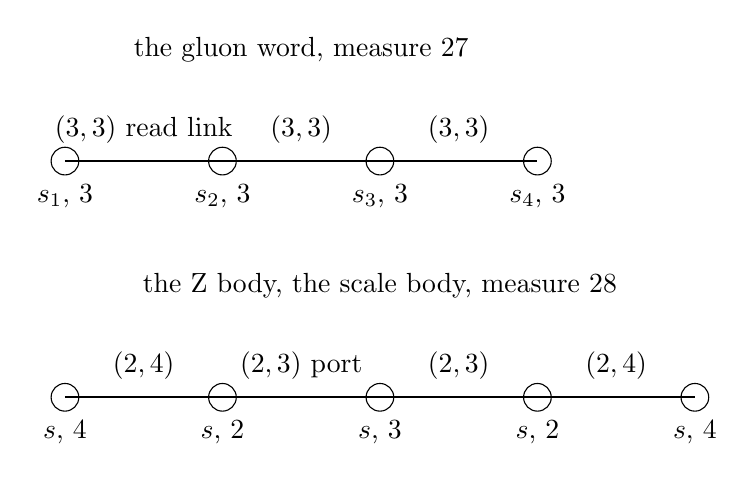
\begin{tikzpicture}[scale=1]
\foreach \x in {0,2,4,6} {\filldraw[fill=white] (\x,0) circle (5pt);}
\draw[thick] (0,0) -- (6,0);
\node at (0,0) [below=5pt] {$s_1$, 3}; \node at (2,0) [below=5pt] {$s_2$, 3}; \node at (4,0) [below=5pt] {$s_3$, 3}; \node at (6,0) [below=5pt] {$s_4$, 3};
\node at (1,0) [above=3pt] {$(3,3)$ read link}; \node at (3,0) [above=3pt] {$(3,3)$}; \node at (5,0) [above=3pt] {$(3,3)$};
\node at (3,1) [above=4pt] {the gluon word, measure $27$};
\foreach \x/\d in {0/4,2/2,4/3,6/2,8/4} {\filldraw[fill=white] (\x,-3) circle (5pt); \node at (\x,-3) [below=5pt] {$s$, \d};}
\draw[thick] (0,-3) -- (8,-3);
\node at (1,-3) [above=3pt] {$(2,4)$}; \node at (3,-3) [above=3pt] {$(2,3)$ port}; \node at (5,-3) [above=3pt] {$(2,3)$}; \node at (7,-3) [above=3pt] {$(2,4)$};
\node at (4,-2) [above=4pt] {the Z body, the scale body, measure $28$};
\end{tikzpicture}\caption{The gluon word with its (3,3) read link and the Z body through which the read is carried by the scale map, with its port.}\end{figure}
\end{chproof}
\par\medskip\noindent{\itshape The carrier of the Part, the photon, is read in the next chapter.}\label{narr:close:5-7}\par
\section{The photon: docking, the join face and pair production}\label{mod:V-8-photon-docking-the-join-face-and-pair-production}
\chdesig{7-8}{5-8}{V-8-photon-docking-the-join-face-and-pair-production}{V-8-D539949-phpk-t1}
\label{narr:open:5-8}Theorem~150.1 reads the photon as docking at both faces, with pair production at the join face, resting on the link, the moves, the saturation, the probe, the constant and the hydrogen chapter.
\begin{chconditional}[The photon docks at both faces]\label{box:V-8-photon-docking-the-join-face-and-pair-production:1}
This result is conditional on the axiom text and on the results of the chapters named as its premises in the derivation below, each at its own standing.
The photon word of the construction, held at both of its ends under the docking act of the axiom text, the qutrit end at the electron dock and the qubit end at the up core by two qutrit-qubit pairs, docks at both of its faces, and the join face that the carrier read of the read link posed as its condition is derived at the dock, the spin content of the read a two-dimensional representation (the doublet).
\end{chconditional}
\chstanding{a conditional theorem}
\chdeps{Definitions 1.1 to 1.6, Theorems 9.1 to 9.7 and Open result 9.8, Theorems 28.1 and 28.2, Open results 28.3 and 28.4 and Theorem 28.5, Theorem 124.1, Theorem 143.1, Open results 241.1 and 241.2, Theorems 241.3 and 241.4 and Open results 241.5 to 241.7 and Open results 245.1 and 245.2, Theorem 245.3, Open results 245.4 to 245.8 and Theorem 245.9}{Theorem 151.1 and Theorem 226.1 and Open result 226.2}
The join face of the photon as the record carries it, the glossary entry of the photon-electron vertex at its typing result, equals the pairing move of the move table applied at the photon, so the join face is the pairing move and no posed face.
Two open results stand here. The closure at the docking face is not derived from the definition of open at the first rung, the parting named at the first test with both faces printed. The hub-forming move of the move table applied to the two standing photon words, the chain of six sites and five links with their open qubit ends paired, does not reach the electron-positron pair as the record carries it, so pair production as the hub-forming move parts as yet. A further open result placed here, the open count at the dock link, is cited at its own standing and compared with nothing.
\begin{chbridge}
The photon is the massless gauge boson of quantum electrodynamics, coupled to the electron current at the vertex $-ie\gamma^{\mu}$ with two transverse polarizations and no longitudinal one \cite{Peskin1995}; pair production in the field of a nucleus is the lowest-order process by which a photon of energy above twice the electron rest energy becomes an electron and a positron, its cross section given by Bethe and Heitler \cite{BetheHeitler1934}. The correspondence is by name.
\end{chbridge}
\begin{chproof}[exact part and census part]
The premises of this derivation are the axiom and the six definitions of chapter~\ref{mod:FRAMEWORK}, the theorem of chapter~\ref{mod:I-2-link-and-its-six-genres}, the theorem of chapter~\ref{mod:I-4-moves-in-one-table}, the theorem of chapter~\ref{mod:I-5-saturation-in-one-figure-seeds-waves-termination-sinks}, the theorem of chapter~\ref{mod:I-6-read-at-a-register-the-probe-and-the-measurement}, the theorem of chapter~\ref{mod:V-1-fine-structure-constant-at-the-one-link} and the theorem of chapter~\ref{mod:V-4-hydrogen-the-rydberg-ladder-and-the-fine-structure}. The chain of premises runs back to the axiom through those chapters, and the longest such chain in this compendium is twelve chapters long.
The held carrier of the hydrogen result is docked at both ends, the dock read of the electron and the up core taken at the qutrit and qubit ends, and the join face of the carrier read derived at the dock from the one-act clause and the join as a contraction of ket and bra ends; the join face is stated from the glossary entry and the typing result, the pairing move of the move table computed at the photon and the two compared. The docking theorem is conditional on the open results it rests on, among them the star as the electron dock read and spin as the doublet content of the read; the join-face theorem rests on the axiom text and the proved results it names alone.
\textit{The exact part.}
From the photon word held at both ends under the docking act (the qutrit end at the electron dock and the qubit end at the up core by two qutrit-qubit pairs), by the two dockings the hydrogen result admits, we obtain the exchange at the two-qubit type hosted at the first dock qubit of the electron with the odd cycle of length two, the mass face at the join six root six against the standing mass face thirty-six.
\begin{equation}
\text{exchange type } (2,2) \ \text{at the host } w_{1}, \qquad M_{\mathrm{join}} = 6\sqrt{6}, \qquad M_{\mathrm{standing}} = 36 .
\end{equation}
From the one-act clause and the join as a contraction of ket and bra ends, by the two-qubit join at the electron dock, we obtain the join face the carrier read posed as its condition, derived at the dock at every one of its thirty-one cells, the spin content of the read a two-dimensional representation.
\begin{equation}
\text{join face} = \text{the } (2,2) \text{ join at the electron dock}, \qquad \dim(\text{spin content}) = 2 .
\end{equation}
\textit{The census part.}
By exhaustive enumeration of the two dockings of the photon word the hydrogen result admits, each built as an exact object under both acts of the derived docking, the photon docks at both of its faces, the dock read of the electron and the up core is taken at the qutrit and qubit ends, the join face of the carrier read is derived at the dock from the one-act clause and the join as a contraction, and the thirty-one cells of the posed join face are re-met at every one. The join face as the glossary entry of the photon-electron vertex carries it equals the pairing move of the move table applied at the photon. The smallest case, the docking at the electron dock, is worked above.
The counter-tests alter the objects singly and read what moves. Docking at one face alone moves the dock, bind, spin and join cells from yes to no with the exchange undefined and the join mass face undefined. The five counter-tests stand at their pinned letters and the sixteen controls read the same at both engines, among them the construction, the figures and the register rule. The result was reproduced by a second engine built apart from the first, the two runs equal at every key.
The machine-checked package named at the reproducibility appendix certifies the statements of this chapter under the definitions of this compendium.
\chcert{31}
\end{chproof}
\begin{figure}[h]\centering
\setlength{\unitlength}{1pt}
\begin{picture}(260,150)
\qbezier(83.4,68.6)(103.5,48.5)(123.6,28.4)
\put(109.2,54.2){\makebox(0,0){\scriptsize $(2,3)$}}
\qbezier(136.4,121.6)(156.5,101.5)(176.6,81.4)
\put(162.2,107.2){\makebox(0,0){\scriptsize $(2,2)$}}
\qbezier(123.6,121.6)(103.5,101.5)(83.4,81.4)
\put(109.2,95.8){\makebox(0,0){\scriptsize $(2,3)$}}
\put(130.0,128.0){\circle{14}}
\put(130.0,128.0){\makebox(0,0){\footnotesize $2$}}
\put(130.0,138.0){\makebox(0,0)[b]{\scriptsize $s_1$}}
\put(77.0,75.0){\circle{14}}
\put(77.0,75.0){\makebox(0,0){\footnotesize $3$}}
\put(77.0,85.0){\makebox(0,0)[b]{\scriptsize $s_6$}}
\put(130.0,22.0){\circle{14}}
\put(130.0,22.0){\makebox(0,0){\footnotesize $2$}}
\put(130.0,32.0){\makebox(0,0)[b]{\scriptsize $w_1$}}
\put(183.0,75.0){\circle{14}}
\put(183.0,75.0){\makebox(0,0){\footnotesize $2$}}
\put(183.0,85.0){\makebox(0,0)[b]{\scriptsize $Q_1$}}
\end{picture}
\caption{The photon word docked at both faces, its qutrit end at the electron dock qubit and its qubit end at the up core, drawn at its two end sites. The two-qubit join at the electron dock supplies the join face of this chapter.}
\end{figure}
\section{The photon as the (2,2) pair ket at the join}\label{mod:V-8-D539949-phpk-t1}
\begin{chtheorem}[The photon as the (2,2) pair ket at the join]\label{box:V-8-D539949-phpk-t1:1}
The office of the (2,2) pair ket at the join under the body-alone rule is zero. The pair ket at the join, a word of two qubit sites and one (2,2) link, the contraction of the pairing move at the qubit ends of two photon reads, the pair of the hub unit and the carrier genre of the electromagnetic, located at four of four parents, is a pendant pair in the dock set of the rule, its act struck at the reading adopted, so its first power is zero, equal to the established first power of the closed read of the photon at the carrier-mass result, its pair part is zero, equal to the first power squared, its closure is zero at its one dark link, and its office is the exact cell zero, the smallest office among the eighteen established offices and equal to the photon object office of the carrier-mass result at both faces and below every other. The genre is bright at the readability result at order one at three faces and the deciding cell, and the two move classes of the electromagnetic, the hub-forming pairing at sixteen edges and the (2,2) join across webs at 31325 edges, are re-met at the forces result with the carrier genre (2,2) at two of two.
The first face, the office of the (2,2) pair ket at the join under the body-alone rule a cell read at order one as a bright genre with its two move classes re-met, the cell zero or the smallest office, reads yes at the reading adopted, located four of four, bright, the office zero and exact with the identity, the smallest, the classes re-met two of two; the second face, the rule refusing a word at the bright genre or the pair ket at the join no word of the construction, reads no, the rule refusing the word at no cell, the pair ket located at every parent and at the fixed library of webs, the first parting none.
\end{chtheorem}
\chstanding{a theorem}
\chdeps{Definitions 1.1 to 1.6 and Theorem 150.1}{no theorem beyond it at this release}
The pair ket at the join is the smallest word of the model that carries the electromagnetic, two qubit sites joined by one (2,2) link of measure four. Under the body-alone rule a link that is a pendant pair at a qubit end belongs to the dock set and its act is struck, so nothing is read along the one link of the word. The first power, the sum of the acts of the unstruck links, is zero. The pair part, the sum over ordered pairs of unstruck links, is zero and equals the square of the first power. The closure at the one dark link is its act multiplied by the link law of its genre, zero. The office, the sum of the three, is the exact cell zero. The same reading at the hub unit, at the pair ket with its two photon reads and at the other established words gives offices that are nonzero elements of the ring, so the office of the pair ket at the join is the smallest of them, and the carrier of the electromagnetic reads at order one as a bright genre whose two move classes are those the forces result names.
\begin{chbridge}
The photon is the massless gauge boson of electrodynamics, the quantum of the electromagnetic field, with zero rest mass and two polarization states, and its masslessness follows in the standard account from the unbroken gauge invariance of the theory \cite{Peskin1995,Weinberg1995}. The correspondence is by name.
\end{chbridge}
\begin{chproof}[finite computation with its exact part]
The premises of this derivation are the axiom and the six definitions of chapter~\ref{mod:FRAMEWORK}, the link and its six genres of chapter~\ref{mod:I-2-link-and-its-six-genres}, a theorem, the photon docking and the join face of chapter~\ref{mod:V-8-photon-docking-the-join-face-and-pair-production}, a theorem, the hub step of chapter~\ref{mod:VI-1-hub-step-as-the-weak-interaction}, a theorem, the mass unit and the first power of chapter~\ref{mod:VIII-1-mass-unit-and-the-first-power}, a theorem, and the body-alone office rule of chapter~\ref{mod:VIII-2-body-alone-office-rule}, a theorem. The chain of premises runs back to the axiom through those chapters, and the longest such chain in this compendium is twelve chapters long.
\textit{The object.} The pair ket at the join is the word of two qubit sites $k_1$ and $k_2$ and one link $k_1k_2$ of genre (2,2), the measure of the link $2\cdot 2=4$, built by the pairing move as the contraction of genre (2,2) at the qubit ends of two photon reads. It is located at four of four parents. At the hub step it stands as the one (2,2) line among the three unit lines $Kk_1$ at (2,4), $Kk_2$ at (2,4) and $k_1k_2$ at (2,2), the pair of the unit never split. At the photon join face it stands as the contraction at the dimensions two and two. At the forces result it stands as the carrier genre of the electromagnetic. At the fixed library of webs it stands as its (2,2) link. Its genre reads bright at order one at the readability result. The figure draws the word and the hub unit it sits in.
\textit{The procedure.} The reading adopted is the measure-struck read with the slot rule, the (3,4)-only dressing, the dark set at the first reading and the link-weight closure. For each link of a word decide whether it lies in the dock set of the rule, a pendant pair at a qubit end does. Strike the act of every dock link. Take the first power $S_1$ as the sum of the acts of the unstruck links, the pair part $P$ as the sum over ordered pairs of unstruck links of the product of their acts, and the closure $C$ as the sum over the dark links of the act multiplied by the link law of the genre. The office is $\Omega = S_1 + P + C$, an element of the ring with the basis one, root two, root three and root six.
\textit{The smallest instance.} The word has one link, $k_1k_2$, a pendant pair at both ends, hence in the dock set with its act struck. The link law of the (2,2) genre is $\tfrac{5}{216} + \tfrac{5}{216}\sqrt{2}$, and the act at the link is zero, so
\begin{equation} S_1 = 0, \qquad P = S_1^{2} = 0, \qquad C = 0\cdot\Big(\tfrac{5}{216} + \tfrac{5}{216}\sqrt{2}\Big) = 0, \qquad \Omega = 0 + 0 + 0 = 0 . \end{equation}
The first power zero equals the first power of the closed read of the photon at the carrier-mass result and its passage first power, both zero; the pair part equals the first power squared, an identity at every read of the grid; the closure is zero at the one dark link; and the office is the exact cell zero, rational, with the identity of the office and its parts holding.
\textit{The exact part.} The same rule at the nine reads of the grid gives the first powers and the offices listed below, each office an exact element of the ring written as its coefficients of one, root two and root three; the office of the pair ket at the join is the smallest, and it equals the photon object office of the carrier-mass result.
\begin{center}\begin{adjustbox}{max width=\linewidth}\begin{tabular}{lrl}\hline read & first power & office \\ \hline the pair ket at the join & 0 & $0$ \\ the pair ket with its two photon reads & 114 & $\tfrac{43118427966377}{3317760000} + \tfrac{649}{4050}\sqrt{2} + \tfrac{5069}{41472000}\sqrt{3}$ \\ the hub unit & 20 & $\tfrac{1458099887}{3645000} + \tfrac{649}{36450}\sqrt{2}$ \\ the photon read, its one (2,3) dock struck & 0 & $0$ \\ the photon word of the library, five (2,3) links & 24 & $576$ \\ the (2,4) free genre & 8 & $\tfrac{466566137}{7290000} + \tfrac{2}{6075}\sqrt{2}$ \\ the W word of the library & 28 & $\tfrac{2857690241}{3645000} + \tfrac{98}{50625}\sqrt{2}$ \\ the Higgs word of the library & 16 & $\tfrac{46656001681}{182250000}$ \\ the electron & 201 & the largest of the nine, at the table of the entry \\ \hline \end{tabular}\end{adjustbox}\end{center}
The two move classes of the electromagnetic at the forces result are the hub-forming pairing, present at sixteen edges with the carriers (2,2), (2,3), (2,4) and (3,4), and the (2,2) join across webs, present at 31325 edges with the carrier (2,2); both carry the genre of the object, both stand among the twenty-eight move ids, and the two re-meet the forces result at two of two.
\textit{The check.} The counter-tests alter the object singly and read what moves. Reading the pair ket at a dark genre, the second qubit struck to a ququart and the link read as (2,4) outside the dock set, gives the first power eight and a nonzero office, twenty cells moved. Keeping the pendant pair in the act read gives the first power four, thirteen cells moved. Striking the (2,2) join class from the located classes parts the re-meet at the count, nine cells moved. Striking the text unmeets the gate, every cell struck. Striking the deciding cell moves twenty-four cells. Each alteration moves the cells it names. The result was reproduced by an independent route, two engines built apart, the keyed-map and fraction route against the array-scan and closed-form route, equal at every cell, with the four control reads of the Higgs-and-carrier offices re-met at four of four and the sixteen controls the same.
\chcert{240}
\begin{figure}[h]\centering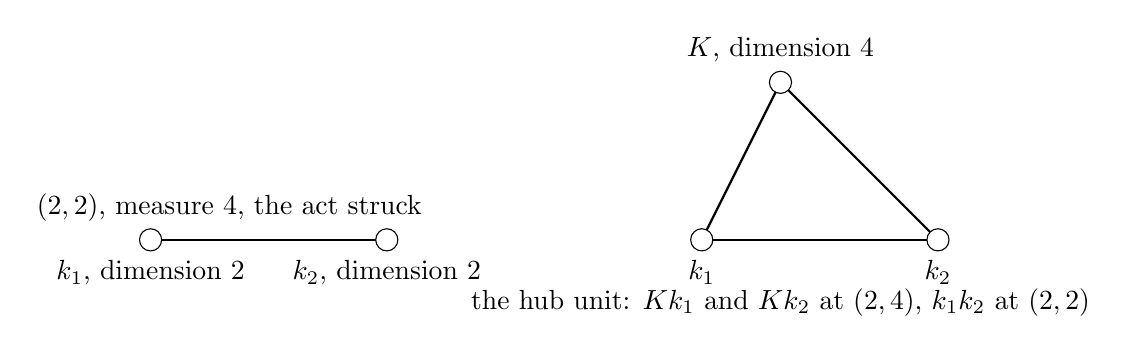
\begin{tikzpicture}[scale=1]
\draw[thick] (0,0) -- (3,0);
\filldraw[fill=white] (0,0) circle (4pt) node[below=4pt] {$k_1$, dimension 2};
\filldraw[fill=white] (3,0) circle (4pt) node[below=4pt] {$k_2$, dimension 2};
\node at (1,0) [above=3pt] {$(2,2)$, measure $4$, the act struck};
\draw[thick] (7,0) -- (10,0);
\draw[thick] (7,0) -- (8,2);
\draw[thick] (10,0) -- (8,2);
\filldraw[fill=white] (7,0) circle (4pt) node[below=4pt] {$k_1$};
\filldraw[fill=white] (10,0) circle (4pt) node[below=4pt] {$k_2$};
\filldraw[fill=white] (8,2) circle (4pt) node[above=4pt] {$K$, dimension 4};
\node at (8,0) [below=14pt] {the hub unit: $Kk_1$ and $Kk_2$ at $(2,4)$, $k_1k_2$ at $(2,2)$};
\end{tikzpicture}\caption{The pair ket at the join, two qubit sites and one (2,2) link, and the hub unit in which it stands as the one (2,2) line.}\end{figure}
\end{chproof}
\par\medskip\noindent{\itshape The next chapter concerns the equation of the charged body at the dock, and is counted empty.}\label{narr:close:5-8}\par
\section{The lepton ladder as hub assemblies}\label{mod:V-10-lepton-ladder-as-hub-assemblies}
\chdesig{7-10}{5-10}{V-10-lepton-ladder-as-hub-assemblies}{V-10-D540869-tthc-t1}
\label{narr:open:5-10}Theorem~152.1 reads the lepton ladder as hub assemblies, resting on the moves, the saturation and the mass unit of chapter 8-1.
\begin{chconditional}[The lepton ladder as hub assemblies]\label{box:V-10-lepton-ladder-as-hub-assemblies:1}
This result is conditional on the axiom text and on the results of the chapters named as its premises in the derivation below, each at its own standing.
At every one of the three lepton webs of the construction the unstruck links are the three coloured core links plus $k$ hub assemblies, each one in-leg, three qubit-ququart legs and one qubit pair at the measure forty, the electron at $k$ one, the muon at two and the tau at three, so the first powers of the ladder are one measure law at three terms.
\end{chconditional}
\chstanding{a conditional theorem}
\chdeps{Definitions 1.1 to 1.6, Theorems 185.1 to 185.12, Open results 241.1 and 241.2, Theorems 241.3 and 241.4 and Open results 241.5 to 241.7 and Open results 245.1 and 245.2, Theorem 245.3, Open results 245.4 to 245.8 and Theorem 245.9}{the theorems of Chapters 1-5, 7-10 to 7-12, 8-2b, 10-1, 10-3 to 10-5, 14-1, 14-6}
The electron body is read by the same rule as every other body and that rule reads it at its hub: the rank of a body, the sum over its links of the end products with the attachments struck, is sixty-seven at the electron, and the read multiplies that rank by its hub product, three at the electron, so the unit of the mass readout stands at 201 at the hub reading and 67 at the dock reading, the two offices parted by the factor nine at every body.
The standing hub step keeps both docks of the electron at both steps, and the muon and tau of the construction are exactly the dock-freed pair readings at the core, every other lowering of the electron isomorphic to none of the lowering classes of the closure of the construction.
With every record of the joined webs of the electron and muon results re-cut at the three record classes of the placement theorem (the position of a tensor in a network), the body-part ratio of the muon to the electron is defined, its interference term an exact nonzero element of the field with a definite sign.
At every qutrit-qubit link of the construction whose qutrit site is the in-end of a qutrit-ququart hub leg, the qutrit end is open as the far end of its hub leg under the definition of open, so the hub leg opens the qutrit end the dock rule closes.
Four open results stand here. The hub as the pair read as one qudit preserves the dressing but consumes the three links of the triangle. The joined read at the ladder of the construction is defined at the electron and the muon and refused at the tau, whose standing attach site is closed. The one rule of the item, the Born count at the open-end set less the struck-dock term multiplied by the hub-leg product, is not the ladder, parting at the muon and the tau. The hub-attached three-quark web read under one rule parts at its first named web. A further open result placed here, every lepton office at its whole sink, is cited at its own standing.
\begin{chbridge}
The three charged leptons of the Standard Model carry the same charge and couplings and differ in mass alone, the three masses three Yukawa couplings fixed by measurement \cite{Weinberg1967}; the generation count three is an input of the model. The correspondence is by name; the record supplies an isometry algebra of the Hermitian split at the Lorentz brackets, a lattice point group, boosts from the order register and a transverse traceless part at the open read, every one a finite or algebraic object of this theory carrying the group name at chapter~\ref{mod:III-2-rotation-group}, chapter~\ref{mod:III-3-lorentz-group-and-the-signature}, chapter~\ref{mod:III-4-boosts-and-the-one-unit}, chapter~\ref{mod:III-5-spin-and-helicity}, the chapter titled Causal structure and general covariance (chapter~\ref{mod:III-8-causal-structure-and-general-covariance}, among the instruments) and chapter~\ref{mod:XIV-7-what-remains-the-ungraded-page}, and the mass corresponds there and here by name.
\end{chbridge}
\begin{chproof}[exact part and census part]
The premises of this derivation are the axiom and the six definitions of chapter~\ref{mod:FRAMEWORK}, the theorem of chapter~\ref{mod:I-4-moves-in-one-table}, the theorem of chapter~\ref{mod:I-5-saturation-in-one-figure-seeds-waves-termination-sinks} and the theorem of chapter~\ref{mod:VIII-1-mass-unit-and-the-first-power}. The chain of premises runs back to the axiom through those chapters, and the longest such chain in this compendium is twelve chapters long.
The rank is summed over the links with the attachments struck and the hub product taken; the two-step readings of the hub step are enumerated at every pure attachment site; the records of the joined webs are re-cut at the three record classes; every qualifying link is typed at the definition of open; and the unstruck links of the three lepton webs are listed and re-met as sets. The body-read theorem is conditional on the open results it rests on, among them the hub dressing at the body; the others rest on the axiom text alone.
\textit{The exact part.}
From the electron web, by listing its unstruck links, we obtain the core triangle of three colored links at the measure twenty-seven and one hub assembly, the in-leg of measure twelve, three qubit-ququart legs of measure twenty-four together and one qubit pair of measure four, the assembly at the measure forty. The two dock links of the qutrit-qubit type are struck at the measure twelve, so the measure and the rank are
\begin{equation}
27 + 40 + 12 = 79, \qquad \operatorname{rank}(e) = 79 - 12 = 67 .
\end{equation}
From the muon and tau webs, by the same listing, we obtain the core triangle plus two and three hub assemblies, the struck docks at measures six and zero and the struck two-qubit leaf links at four and eight, so the measures step as
\begin{equation}
27 + 2 \cdot 40 + 6 + 4 = 117, \qquad 27 + 3 \cdot 40 + 0 + 8 = 155, \qquad \operatorname{rank}(\mu) = 107, \quad \operatorname{rank}(\tau) = 147 ,
\end{equation}
the ranks stepping by forty at both steps, equal to the hub-assembly measure, so the first powers of the ladder are one measure law at three terms.
\begin{equation}
\operatorname{rank}(\ell_{k}) = 27 + 40\,k, \qquad k = 1, 2, 3 .
\end{equation}
\textit{The census part.}
By exhaustive enumeration of the links of the three lepton webs of the construction at both readings of the docks, every unstruck link is assigned to the core triangle or to one hub assembly (each one in-leg, three qubit-ququart legs and one qubit pair at the measure forty) with no link assigned to none at either reading, the electron at one assembly, the muon at two and the tau at three. The rank is summed over the links with the attachments struck and the hub product taken, and the first powers of the ladder re-met as sets. The smallest case, the electron web, is worked above.
The counter-tests alter the objects singly and read what moves. Striking one assembly moves all nine of its cells, the first the dock of the electron. The four counter-tests stand at their pinned letters and the ten controls read the same at both engines, every consumed file unaltered. The result was reproduced by a second engine built apart from the first, the two runs equal at every one of the cells of both.
The machine-checked package named at the reproducibility appendix certifies the statements of this chapter under the definitions of this compendium.
\chcert{3}
\end{chproof}
\begin{figure}[h]\centering
\setlength{\unitlength}{1pt}
\begin{picture}(260,150)
\qbezier(121.5,124.9)(113.0,121.8)(104.4,118.7)
\put(115.7,114.3){\makebox(0,0){\scriptsize $(3,3)$}}
\qbezier(91.4,107.8)(86.9,99.9)(82.3,92.0)
\put(93.8,95.9){\makebox(0,0){\scriptsize $(3,3)$}}
\qbezier(84.7,90.0)(103.9,106.1)(123.1,122.2)
\put(98.8,112.2){\makebox(0,0){\scriptsize $(3,3)$}}
\qbezier(88.6,56.3)(107.1,88.2)(125.5,120.2)
\put(100.1,92.2){\makebox(0,0){\scriptsize $(3,4)$}}
\qbezier(91.0,42.7)(98.0,36.8)(105.0,31.0)
\put(103.1,43.0){\makebox(0,0){\scriptsize $(2,4)$}}
\qbezier(92.6,45.4)(116.1,36.8)(139.7,28.3)
\put(118.9,44.4){\makebox(0,0){\scriptsize $(2,4)$}}
\qbezier(93.1,48.5)(130.0,48.5)(166.9,48.5)
\put(130.0,56.5){\makebox(0,0){\scriptsize $(2,4)$}}
\qbezier(120.9,25.2)(130.0,25.2)(139.1,25.2)
\put(130.0,33.2){\makebox(0,0){\scriptsize $(2,2)$}}
\qbezier(104.4,112.5)(139.1,99.9)(173.7,87.3)
\put(141.8,107.4){\makebox(0,0){\scriptsize $(2,3)$}}
\qbezier(86.3,87.3)(120.9,99.9)(155.6,112.5)
\put(118.2,107.4){\makebox(0,0){\scriptsize $(2,3)$}}
\put(130.0,128.0){\circle{14}}
\put(130.0,128.0){\makebox(0,0){\footnotesize $3$}}
\put(130.0,138.0){\makebox(0,0)[b]{\scriptsize $A$}}
\put(95.9,115.6){\circle{14}}
\put(95.9,115.6){\makebox(0,0){\footnotesize $3$}}
\put(95.9,125.6){\makebox(0,0)[b]{\scriptsize $B$}}
\put(77.8,84.2){\circle{14}}
\put(77.8,84.2){\makebox(0,0){\footnotesize $3$}}
\put(77.8,94.2){\makebox(0,0)[b]{\scriptsize $C$}}
\put(84.1,48.5){\circle{14}}
\put(84.1,48.5){\makebox(0,0){\footnotesize $4$}}
\put(84.1,58.5){\makebox(0,0)[b]{\scriptsize $H$}}
\put(111.9,25.2){\circle{14}}
\put(111.9,25.2){\makebox(0,0){\footnotesize $2$}}
\put(111.9,35.2){\makebox(0,0)[b]{\scriptsize $g_1$}}
\put(148.1,25.2){\circle{14}}
\put(148.1,25.2){\makebox(0,0){\footnotesize $2$}}
\put(148.1,35.2){\makebox(0,0)[b]{\scriptsize $g_2$}}
\put(175.9,48.5){\circle{14}}
\put(175.9,48.5){\makebox(0,0){\footnotesize $2$}}
\put(175.9,58.5){\makebox(0,0)[b]{\scriptsize $g_3$}}
\put(182.2,84.2){\circle{14}}
\put(182.2,84.2){\makebox(0,0){\footnotesize $2$}}
\put(182.2,94.2){\makebox(0,0)[b]{\scriptsize $w_1$}}
\put(164.1,115.6){\circle{14}}
\put(164.1,115.6){\makebox(0,0){\footnotesize $2$}}
\put(164.1,125.6){\makebox(0,0)[b]{\scriptsize $w_2$}}
\end{picture}
\caption{The electron web as the core triangle plus one hub assembly, the three qutrit core sites, the hub of dimension four with its in-leg, its three qubit legs and the qubit pair, and the two dock qubits whose links are struck. Each site labeled by its dimension and each link by its pair type.}
\end{figure}
\section{The lepton block at the unwashed port overlap}\label{mod:V-10-D539519-w-tflb}
The mixing of the three lepton generations is a unitary three-by-three block relating the flavour states to the mass states of the neutral partners, parametrised by three angles and a phase, its single rephasing-invariant measure of CP violation the Jarlskog invariant; the block is unitary on three when the neutral partners are three alone, and a fourth column would mark a further state \cite{Pontecorvo1958,Maki1962,Jarlskog1985}. The lepton ladder as hub assemblies is introduced at section~\ref{mod:V-10-lepton-ladder-as-hub-assemblies} and the mixing with the washed overlap at section~\ref{mod:VI-7-mixing-the-washed-overlap-and-the-ckm-block}.
The three-by-three block of the lepton overlap at the three read sites, with the dark end as a fourth column, is cut unwashed at the open ports: the dock read of the charged partner against the port read at the hub register, every far end of the hub open at the hub read at 20 of 20 letter and far-end pairs, the frame test and the dimension test agreeing, and the wash applied at no open port. Cut at every one of the six hub assemblies of the standard lepton webs and every one of the 20 letter pairs, the unwashed block is unitary at the base criterion at 4 of 20 pairs and flat at 7 of 20.
The six assemblies are lined up with the three cross-core webs by the hub count at 3 of 3. Among the 20 pairs one block is a unitary with distinct moduli, the Jarlskog cell is nonzero at none of them and a single value at 9 of 20, and the block phases fall inside the phase group of the (3,3) genre at 76 of 165 with the cycles exact at 9 of 20. The washed block of the standing result, unitary at 0 of 20 and flat at 20 of 20, the unread-end reading, unitary at 4 of 20, and the port-typed reading each stand at their own second face. The first parting is the first assembly, the electron hub at the letter pair Z against X with the dark-end column at the third leg: there the block is flat and not unitary, its Born block one quarter at every entry with the row sums three quarters, its Gram matrices parting from the identity, and its Jarlskog cell one sixteenth with the square 1 over 256; the second value named is the first block phase outside the phase group. Two independent implementations agree at every value and the runs are byte-identical.
The result is an open one, an open result: the stronger statement, that the unwashed block at the open ports is unitary on three, is not met, and the weaker statement is named with both values; no comparison with observation is made here.
What stays open is the reading of this block together with the washed block carrying the dark-end column (section~\ref{mod:VI-7-D539152-w-lmde}) and with the muon ports under the derived definition (the chapter titled The muon ports under the derived definition of open (chapter~\ref{mod:VI-2a-D539543-mprt-t1}, among the instruments)), which no result has made.
\section{The tau as the third hub on the triangle core}\label{mod:V-10-D540869-tthc-t1}
\begin{chtheorem}[The tau as the third hub on the triangle core]\label{box:V-10-D540869-tthc-t1:1}
The tau as the third hub on the triangle core, at its second face: no isomorph of the triangle-plus-one web built from the muon web of the fixed library stands among the three hundred three-hub lepton-form sinks of the tau census, zero of three hundred at the reading adopted, at the leaf reading and at the star reading; its own Koide ratio at the first powers lies outside the band of one part in a thousand of two thirds, 9336401 over 13739282 at the first power 4212, as does every one of the three hundred, zero of three hundred inside; the nearest candidate of the triangle-plus-one kind is the sink at the first power 3996 and the ratio 8449937 over 12630338, the nearest of the star kind the tau sink itself at 4185 and 18446083 over 27196225; so the second face holds, absent or outside with the nearest candidates named with both cells, and the first face fails, every cell an exact element of the ring compared with the canonical two thirds alone.
The first face, an isomorph of the triangle-plus-one web present among the three hundred with its Koide ratio inside the band, reads no, no isomorph present and none inside; the second face, absent or outside with the nearest candidates named, reads yes at the first basis of the search, the isomorphism absent at zero of three hundred and the ratio outside at every sink.
\end{chtheorem}
\chstanding{a theorem}
\chdeps{Definitions 1.1 to 1.6 and Theorem 152.1}{no theorem beyond it at this release}
The question was whether the tau is the muon web grown by one more hub on its triangle core, the third generation as the third hub. The web that reading builds, eighteen sites and twenty-one links with three hubs of degree four on a core of four qutrits, is compared site by site and link by link with every three-hub lepton-form sink of the tau census, and none of the three hundred is that web under any bijection of sites that keeps the dimensions and the genres of the links; the tau sink identified by the identification standard, a star core of sixteen sites, is not that web either. The Koide ratio, the sum of the squares of the three first powers over the square of their sum with the electron at 67 and the muon at 963, is an exact rational at every sink, and it lies outside a band of one part in a thousand around two thirds at every one of them and at the triangle-plus-one web itself, so the reading supplies neither the tau nor the Koide relation, and the result names the nearest candidates of each core kind with both of their cells.
\begin{chbridge}
The tau is the third charged lepton, the heaviest of the three generations, and the Koide relation is the empirical statement that the sum of the three charged-lepton masses is two thirds of the square of the sum of their square roots, a relation with no derivation in the Standard Model, where the lepton masses are Yukawa couplings fixed by measurement \cite{Koide1983,Weinberg1995}. The correspondence is by name.
\end{chbridge}
\begin{chproof}[finite computation]
The premises of this derivation are the axiom and the six definitions of chapter~\ref{mod:FRAMEWORK}, the lepton ladder as hub assemblies of chapter~\ref{mod:V-10-lepton-ladder-as-hub-assemblies}, a theorem, the body-alone office rule of chapter~\ref{mod:VIII-2-body-alone-office-rule}, a theorem, the dressing as the unpassed (3,4) in-legs of chapter~\ref{mod:VIII-1-mass-unit-and-the-first-power}, a theorem, and the Koide class of chapter~\ref{mod:V-12-koide-class}, an open result. The chain of premises runs back to the axiom through those chapters, and the longest such chain in this compendium is twelve chapters long.
\textit{The procedure.} The input objects are the generation-step web, built from the muon web of the fixed library by keeping its triangle core, placing a fourth qutrit on the corner and attaching a third hub with its legs as the first muon hub carries them, and the three hundred three-hub lepton-form sinks of the tau census, each located at its state row by face, wave and id in the seven state files of that census. For every sink the census cells, the sites, links, measure, docks and hubs, are re-read and the core kind, the dock count, the in-leg count, the dressing, the rank, the first power at the wave-zero reading of the body-alone rule and the office are computed. The test applied to each sink is twofold: whether some bijection of its sites onto the sites of the generation-step web preserves the dimension of every site and the genre-labeled adjacency of every link, searched depth first by the first engine and by backtracking placement by the second, at three readings of the third hub; and whether its Koide ratio lies within one part in a thousand of two thirds. The aggregation counts the isomorphs and the sinks inside the band and names the nearest candidate of each core kind by its distance.
\textit{The objects at their cells.} The generation-step web has 18 sites, 11 qubits, 4 qutrits and 3 ququarts, 21 links at the genres (2,2) four, (2,3) one, (2,4) nine, (3,3) four and (3,4) three, the measure 166, three hubs of degree four, three in-legs and the dressing 27, one dock at the first reading and the dock set of measure 10, the core of four qutrits on four (3,3) links, the rank 156 and the first power 4212. The three hundred sinks fall into the core kinds star 88, triangle-plus-one 87, four-cycle-plus-one 0 and other 125, the last being 114 triangles and 11 three-qutrit paths; their dressings are 3 at 199 sinks, 9 at 88 and 27 at 13, and their first powers run from 369 to 4617 at 63 distinct values.
\textit{The smallest instance.} The Koide ratio at the generation-step web itself, with the electron and the muon first powers 67 and 963 and its own first power 4212, is
\begin{equation} \frac{67^{2} + 963^{2} + 4212^{2}}{(67 + 963 + 4212)^{2}} = \frac{4489 + 927369 + 17740944}{5242^{2}} = \frac{18672802}{27478564} = \frac{9336401}{13739282}, \end{equation}
and its distance from two thirds is
\begin{equation} \frac{2}{3} - \frac{9336401}{13739282} = \frac{27478564 - 28009203}{41217846} = -\frac{530639}{41217846}, \end{equation}
outside the band, since one part in a thousand of two thirds is 1 over 1500 and 530639 over 41217846 exceeds it. The same arithmetic at the sink of the triangle-plus-one kind with the first power 3996 gives the ratio 8449937 over 12630338 at the distance 89135 over 37891014, the nearest overall, and at the tau sink of the star kind with the first power 4185 the ratio 18446083 over 27196225 at the distance 945799 over 81588675, both outside.
\textit{The result.} The isomorphism search finds the generation-step web present at 0 of 300 at the reading adopted, 34 sinks sharing its site and link counts and none a map, at 0 of 300 at the leaf reading, 41 at its counts, and at 0 of 300 at the star reading, 6 at its counts; the tau sink of sixteen sites parts from the web at the site counts, 16 against 18, with zero maps at every reading. The control pairs re-meet the identity engines, the electron sink onto the two-dock web the same at four maps, the muon sink onto the muon web the same at four maps, and the tau sink against the tau web parting at zero maps. The sinks inside the band number 0 of 300. So the second face holds and the first fails, and the theorem states the second face with the nearest candidates named.
\textit{The check.} The counter-tests alter the inputs singly and read what moves. Replacing the generation-step web by the tau web of the fixed library at the search moves the site count of the search. Widening the band to one part in ten moves the count of sinks inside. Replacing the reference first powers by the body-alone first powers of the library webs moves the Koide cells. Striking the text unmeets the gate. Each alteration moves the cells it names. The result was reproduced by an independent route, two engines built apart, the depth-first search against the backtracking placement, equal at every cell, the two-read identity re-met at nine of nine reads and three hundred of three hundred sinks and the fourteen controls the same.
\chcert{300}
\end{chproof}
\par\medskip\noindent{\itshape The ladder in hand, the next chapter reads the dissolution of a face and the exponent it leaves.}\label{narr:close:5-10}\par
\section{The face dissolution, the leg count and the exponent}\label{mod:V-11-face-dissolution-the-leg-count-and-the-exponent}
\chdesig{7-11}{5-11}{V-11-face-dissolution-the-leg-count-and-the-exponent}{V-11-D543290-w-grfn}
\label{narr:open:5-11}Theorem~155.1 is the face dissolution theorem, with the leg count and the exponent, resting on the mass unit and the lepton ladder.
\begin{chconditional}[The face dissolution theorem]\label{box:V-11-face-dissolution-the-leg-count-and-the-exponent:1}
This result is conditional on the axiom text and on the results of the chapters named as its premises in the derivation below, each at its own standing.
The two readings of the mass law, the dock reading and the hub reading, are one law up to the unit absorbing one leg at every established result, the ratio form carries no reading, and the reading word is dissolved with its residue the leg function as a corollary.
\end{chconditional}
\chstanding{a conditional theorem}
\chdeps{Definitions 1.1 to 1.6, Theorem 152.1 and Theorems 185.1 to 185.12}{Open result 156.1 and Theorems 198.1 to 198.3 and Open results 198.4 and 198.5}
The standing two-dock act, named from the electron of the construction, its two docks and its hub with the carry from the hub reaching both docks at once as the far ends, transported to the two-port neutral object reaches every cross-core port, all six at the three cross-core webs and all twenty at the ten objects, and names the reading by the arrows alone at all three generations, the same reading at the first and the third and the opposite at the second.
The in-leg count is one function of the web alone, invariant under every reading and equal to the established $k$ at every result, so the leg count is a definition, the two open questions of the reading dissolved as questions of the reading and the first-power law carrying $k$ by construction.
Four open results stand here. The result that fixes the arrows at the fourteen sinks of the pairing move reaches no port of the three cross-core webs, so the face at the cross-core ports is undefined at those arrows at all three generations. The generator of the step (the step generator) at the first parting tabulated link parts from the factor six multiplied by the order operator lifted to the link register, the first parting register the one link itself. The strike rule that a dock is struck exactly when it is the probe attach site reproduces the struck set at no tabulated lepton result. The probe read placed at the attach dock and carried through the web enters a hub through its qutrit at some webs and through a qubit copy at others, so the leg count read by the act is free at the first web named. Two further open results placed here, the strike as a sector and the strike rule per body at the typed cap, are cited at their own standing and compared with nothing.\textsuperscript{,}
\begin{chbridge}
In the Standard Model a mass term is written once, at the Lagrangian, and carries no choice of reading: the fermion mass is the coefficient of the bilinear in the field and its conjugate, the same number at every frame and at every basis of the fields \cite{Weinberg1967}, and the exponent of the mass in an amplitude is fixed by the dimension of the operator and by nothing else. The correspondence is by name; the record supplies a finite re-matching group at the known clause, a representation census at the open ends and the sinks, an attach-site basis carrying the generation name and a sink class carrying the doublet name at chapter~\ref{mod:IV-1-gauge-invariance-as-the-known-clause}, chapter~\ref{mod:IV-3-representations-from-the-open-end-census}, chapter~\ref{mod:IV-4-cartan-weights-and-the-charge}, chapter~\ref{mod:IV-6-conservation-as-the-kernel-of-the-move-matrix}, chapter~\ref{mod:IV-7-noether-at-the-sinks-and-the-kernel-identification}, chapter~\ref{mod:IV-9-one-rule-of-a-read-and-the-word-table}, chapter~\ref{mod:VI-3-doublets-handedness-and-parity-violation}, chapter~\ref{mod:VII-7-quark-content-and-flavour}, chapter~\ref{mod:VIII-4-three-generations-as-attach-sites} and chapter~\ref{mod:XIV-7-what-remains-the-ungraded-page}, and the generation count and the generation correspond there and here by name.
\end{chbridge}
\begin{chproof}[exact part, finite part and census part]
The premises of this derivation are the axiom and the six definitions of chapter~\ref{mod:FRAMEWORK}, the theorem of chapter~\ref{mod:VIII-1-mass-unit-and-the-first-power} and the theorem of chapter~\ref{mod:V-10-lepton-ladder-as-hub-assemblies}. The chain of premises runs back to the axiom through those chapters, and the longest such chain in this compendium is twelve chapters long.
The two-dock act is named from the electron of the construction, transported to the two-port neutral object and carried to every cross-core port with the reading read off the arrows at every generation; the dock reading and the hub reading of the mass law are compared at every established result; and the in-leg count is computed as a function of the web alone at every reading and re-met at the established $k$; every theorem rests on the axiom text and the proved results it names alone, and the open results are readings the derivation tried and parted at their named steps.
\textit{The exact part.}
From the two readings of the mass law at the electron, the dock reading at the dock-struck first power sixty-seven and the hub reading at the hub first power two hundred and one, by the ratio of the two units, we obtain the parting three at the first power and nine at the square, equal to the hub unit over the dock unit and its square, the unit absorbing one leg and nothing else, the electron at one over one at either face.
\begin{equation}
\frac{201}{67} = 3, \qquad \Big(\frac{201}{67}\Big)^{2} = 9, \qquad r_{e}^{\mathrm{dock}} = r_{e}^{\mathrm{hub}} = \tfrac{1}{1} .
\end{equation}
From every established cell of the parent results typed to its face (the dock face the row at the measure multiplied by three to the power $k$ over sixty-seven, the hub face at three to the power $k$ plus one over two hundred and one, the mixed face the hub numerator over the dock unit), by the computed cell against the established cell, we obtain equality at every one, so the two readings are one law up to the unit absorbing one leg.
\begin{equation}
\text{dock: } \frac{M \cdot 3^{k}}{67}, \qquad \text{hub: } \frac{M \cdot 3^{k+1}}{201}, \qquad \frac{M \cdot 3^{k+1}}{201} = \frac{M \cdot 3^{k}}{67} .
\end{equation}
\textit{The finite part.}
The procedure. Name the two-dock act from the electron of the construction, its two docks and its hub with the carry from the hub reaching both docks at once as the far ends. Transport it to the two-port neutral object and carry it to every cross-core port, reading the reading off the arrows at every generation. Compare the dock reading and the hub reading of the mass law at every established cell of the parents, typed to its face, and compute the in-leg count as a function of the web alone at every reading and re-meet it at the established $k$. The smallest instance, the electron at both faces, is worked above, the fifty established cells of the parents are typed to their faces and the computed cell equals the established cell at every one, the in-leg count one at the electron, two at the muon and three at the tau.
\textit{The census part.}
By exhaustive enumeration of the cross-core ports of the three cross-core webs (six) and of the ten objects (twenty), the transported two-dock act reaches every port and names the reading by the arrows alone at all three generations, the same reading at the first and the third and the opposite at the second. The leg count is one function of the web alone, invariant under every reading.
The counter-tests alter the objects singly and read what moves. The hub unit taken at two legs moves all twelve of its cells, the first the hub of the electron. The four counter-tests stand at their pinned letters and the ten controls read the same at both engines, every consumed file unaltered. The result was reproduced by a second engine built apart from the first, the two runs equal at every one of the cells of both.
The machine-checked package named at the reproducibility appendix certifies the statements of this chapter under the definitions of this compendium.
\chcert{50}
\end{chproof}
\begin{figure}[h]\centering
\setlength{\unitlength}{1pt}
\begin{picture}(260,150)
\qbezier(127.2,119.4)(114.4,80.1)(101.6,40.7)
\put(122.0,77.6){\makebox(0,0){\scriptsize $(3,3)$}}
\qbezier(122.7,122.7)(104.8,109.7)(86.9,96.7)
\put(109.5,103.2){\makebox(0,0){\scriptsize $(2,3)$}}
\qbezier(107.8,32.1)(130.0,32.1)(152.2,32.1)
\put(130.0,40.1){\makebox(0,0){\scriptsize $(2,3)$}}
\qbezier(173.1,96.7)(155.2,109.7)(137.3,122.7)
\put(150.5,103.2){\makebox(0,0){\scriptsize $(3,4)$}}
\put(130.0,128.0){\circle{14}}
\put(130.0,128.0){\makebox(0,0){\footnotesize $3$}}
\put(130.0,138.0){\makebox(0,0)[b]{\scriptsize $B$}}
\put(79.6,91.4){\circle{14}}
\put(79.6,91.4){\makebox(0,0){\footnotesize $2$}}
\put(79.6,101.4){\makebox(0,0)[b]{\scriptsize $w_1$}}
\put(98.8,32.1){\circle{14}}
\put(98.8,32.1){\makebox(0,0){\footnotesize $3$}}
\put(98.8,42.1){\makebox(0,0)[b]{\scriptsize $C$}}
\put(161.2,32.1){\circle{14}}
\put(161.2,32.1){\makebox(0,0){\footnotesize $2$}}
\put(161.2,42.1){\makebox(0,0)[b]{\scriptsize $w_2$}}
\put(180.4,91.4){\circle{14}}
\put(180.4,91.4){\makebox(0,0){\footnotesize $4$}}
\put(180.4,101.4){\makebox(0,0)[b]{\scriptsize $H$}}
\end{picture}
\caption{The two-dock act named from the electron, its two dock qubits and its hub of dimension four, the carry from the hub reaching both docks at once as the far ends. Each site labeled by its dimension and each link by its pair type.}
\end{figure}
\section{The Green function and the falloff exponent at the (2,2) web}\label{mod:V-11-D543290-w-grfn}
\begin{chwall}[The Green function and the falloff exponent at the (2,2) web]\label{box:V-11-D543290-w-grfn:1}
The (2,2) two-point function of the second-order law between two bodies falls as the first power of the separation along a serial (2,2) chain and not as a power where the chain carries a (2,3) link. At the chains of the electron, the muon, the tau, the neutron seed and the W word, whose link is a (2,2) link, the two-point function is $\tfrac{30 + 30\sqrt{2}}{2304}$ multiplied by the separation at every established separation one to four and beyond to twelve, the ratios of successive separations $1/2$, $2/3$ and $3/4$, the exponent one and the effective dimension three; at the chains of the proton sink and the photon word, whose link is a (2,3) link kept at its genre beside the inserted (2,2) links, the two-point function is $\tfrac{79 + 48\sqrt{2} + 42\sqrt{3} + 3\sqrt{6}}{31104 + 2304\,(k-1)}$ at the separation $k$, the ratios $27/29$, $29/31$ and $31/33$, no exact exponent; the (2,3) charge through the (2,2) carrier falls at the exponent one, equal; the first parting is the chain of the proton sink at the separation two; both faces printed.
The first face, the two-point function exact at every chain and established step, the falloff a fixed power with an exact exponent at every chain and beyond, and the (2,3) exponent equal to the (2,2) exponent, reads no, the falloff no fixed power at the chains of the proton sink and the photon word; the second face, otherwise with the first parting named in the order of the item, reads yes, the first parting the ratio of successive separations at the chain of the proton sink at the separation two, the register 33408 against 31104 at the separation one, no multiple of the separation. Open is the falloff where the chain carries a link of another genre: the register of that link adds a constant to the register of the chain and the two-point function is then no power of the separation.
\end{chwall}
\chstanding{an open result}
\chdeps{Definitions 1.1 to 1.6 and Theorem 155.1}{no theorem beyond it at this release}
Two bodies are joined by a chain of links of genre (2,2) of length $k$, the separation, and the two-point function of the second-order law between them is read as the register sum at the ends over the register of the chain. By the additive law of the registers the register of a serial (2,2) chain is the register of one (2,2) link multiplied by $k$, so the function is a constant over $k$, a first-power falloff whose effective dimension is three. Where the chain of a body carries a (2,3) link, as the proton sink and the photon word do, that link adds its own register as a constant, the register of the chain is no multiple of the separation, and the ratio of successive separations is no fixed power, which the result names as the first parting. The (2,3) charge carried through the (2,2) chain falls at the same first power.
\begin{chbridge}
The Green function of a massless field in three spatial dimensions falls as the inverse first power of the separation, the Coulomb law, and the exponent of a two-point function fixes the effective dimension of the space it propagates in \cite{Jackson1998,Peskin1995}. The correspondence is by name.
\end{chbridge}
\begin{chproof}[finite computation with its exact part]
The premises of this derivation are the axiom and the six definitions of chapter~\ref{mod:FRAMEWORK}, the link and its six genres of chapter~\ref{mod:I-2-link-and-its-six-genres}, a theorem, the face dissolution, the leg count and the exponent of chapter~\ref{mod:V-11-face-dissolution-the-leg-count-and-the-exponent}, a theorem, the curvature as the graph Laplacian of chapter~\ref{mod:X-1-curvature-as-the-graph-laplacian-washed-over-the-ladder}, a theorem, and the Ward functional and the dressing per unit of chapter~\ref{mod:V-1-fine-structure-constant-at-the-one-link}, an open result. The chain of premises runs back to the axiom through those chapters, and the longest such chain in this compendium is twelve chapters long.
\textit{The object.} A serial (2,2) chain of separation $k$ joins two bodies at the ends of the designated link of each chain of the serial insertion result, seven chains, five with a designated (2,2) link and two, the proton sink with its link $s_{1}s_{4}$ at (2,3) and the photon word with its link $s_{2}s_{3}$ at (2,3), with a (2,3) link kept at its genre beside the inserted (2,2) links. The figure draws a chain of each kind.
\textit{The procedure.} Re-derive the (2,2) two-point function at the one link by the census polynomials at the end dimensions two and two: the 57 records in the sectors odd 24, mixed-even 18, same-even 12 and closure 3, the register sum $30 + 30\sqrt{2}$ at the root rule, the register 2304 and the cap 96; read the (2,2) center on the pair ket. For each chain and each separation $k$ from one to the established four and beyond to twelve, take the register of the chain by the additive law, the registers of its links at their genres added, and the two-point function as the register sum at the ends over that register; take the ratio of the function at successive separations and ask whether it is one fixed power of $k$; and read the (2,3) count of the Ward-functional entry through the same chains.
\textit{The smallest instance.} At the one (2,2) link,
\begin{equation} g_{1} = \frac{30 + 30\sqrt{2}}{2304}, \qquad \text{the center on the pair ket at the scalar } 0, \end{equation}
equal to the cell of the (2,2) two-point-function result, the count at the acting center $0/2304$ and at the unit functional $g_{1}$. Along a serial (2,2) chain of separation $k$ the register is $2304\,k$, so
\begin{equation} g_{k} = \frac{30 + 30\sqrt{2}}{2304\,k}, \qquad \frac{g_{2}}{g_{1}} = \frac{1}{2}, \quad \frac{g_{3}}{g_{2}} = \frac{2}{3}, \quad \frac{g_{4}}{g_{3}} = \frac{3}{4}, \end{equation}
the exponent one and the effective dimension three, at the five chains with a designated (2,2) link and at the two chains beside, at every separation to twelve. At the chain of the proton sink the register at the separation $k$ is $31104 + 2304\,(k-1)$, the (2,3) register of its link plus the (2,2) register per inserted link, so
\begin{equation} g_{k}^{P} = \frac{79 + 48\sqrt{2} + 42\sqrt{3} + 3\sqrt{6}}{31104 + 2304\,(k-1)}, \qquad \frac{g_{2}^{P}}{g_{1}^{P}} = \frac{31104}{33408} = \frac{27}{29}, \quad \frac{29}{31}, \quad \frac{31}{33}, \end{equation}
no exact exponent, the first parting at the separation two; the photon word parts alike. The (2,3) count $\tfrac{79 + 48\sqrt{2} + 42\sqrt{3} + 3\sqrt{6}}{31104}$ read through the (2,2) carrier at the separation gives the ratios $1/2$, $2/3$ and $3/4$, the exponent one, equal to the (2,2) exponent.
\textit{The check.} The counter-tests alter the construction singly and read what moves. Striking a link of the chain refuses the one-link chain and leaves no fixed power at the electron chain. Reading a (2,3) chain in place of the (2,2) moves the one-link register from 2304 to 31104 and the center scalar from zero to one. Transposing the pair ket moves the scalar of the (2,2) center from zero to two, acting, and the count at the acting center to a nonzero element. Reading the separation zero refuses every two-point function. Striking the text unmeets the gate. Each alteration moves the cells it names. The result was reproduced by an independent route, two engines built apart, the keyed-map and fraction route against the array route, equal at every cell, with the thirteen controls the same.
\chcert{57}
\begin{figure}[h]\centering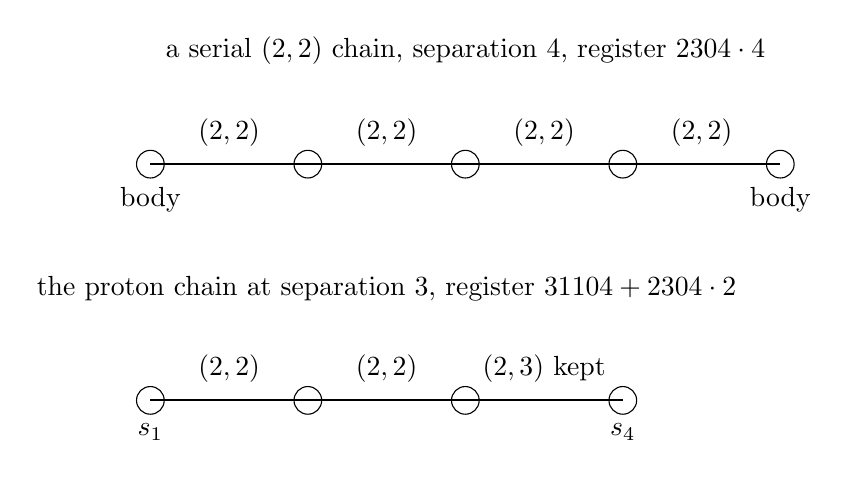
\begin{tikzpicture}[scale=1]
\foreach \x in {0,2,4,6,8} {\filldraw[fill=white] (\x,0) circle (5pt);}
\draw[thick] (0,0) -- (8,0);
\node at (0,0) [below=5pt] {body}; \node at (8,0) [below=5pt] {body};
\node at (1,0) [above=3pt] {$(2,2)$}; \node at (3,0) [above=3pt] {$(2,2)$}; \node at (5,0) [above=3pt] {$(2,2)$}; \node at (7,0) [above=3pt] {$(2,2)$};
\node at (4,1) [above=4pt] {a serial $(2,2)$ chain, separation $4$, register $2304\cdot 4$};
\foreach \x in {0,2,4,6} {\filldraw[fill=white] (\x,-3) circle (5pt);}
\draw[thick] (0,-3) -- (6,-3);
\node at (0,-3) [below=5pt] {$s_1$}; \node at (6,-3) [below=5pt] {$s_4$};
\node at (1,-3) [above=3pt] {$(2,2)$}; \node at (3,-3) [above=3pt] {$(2,2)$}; \node at (5,-3) [above=3pt] {$(2,3)$ kept};
\node at (3,-2) [above=4pt] {the proton chain at separation $3$, register $31104 + 2304\cdot 2$};
\end{tikzpicture}\caption{A serial (2,2) chain between two bodies, whose register is a multiple of the separation, and the chain of the proton sink, whose (2,3) link adds a constant.}\end{figure}
\end{chproof}
\begin{figure}[htbp]\centering
\setlength{\unitlength}{1mm}
\begin{picture}(164,61)(0,0)
\put(8,6){\line(1,0){146}}
\put(10,6){\framebox(4,2){}}\put(15,6){\rule{4mm}{27mm}}\put(14,2){\makebox(0,0){\tiny 1}}
\put(22,6){\framebox(4,4){}}\put(27,6){\rule{4mm}{29mm}}\put(26,2){\makebox(0,0){\tiny 2}}
\put(34,6){\framebox(4,6){}}\put(39,6){\rule{4mm}{31mm}}\put(38,2){\makebox(0,0){\tiny 3}}
\put(46,6){\framebox(4,8){}}\put(51,6){\rule{4mm}{33mm}}\put(50,2){\makebox(0,0){\tiny 4}}
\put(58,6){\framebox(4,10){}}\put(63,6){\rule{4mm}{35mm}}\put(62,2){\makebox(0,0){\tiny 5}}
\put(70,6){\framebox(4,12){}}\put(75,6){\rule{4mm}{37mm}}\put(74,2){\makebox(0,0){\tiny 6}}
\put(82,6){\framebox(4,14){}}\put(87,6){\rule{4mm}{39mm}}\put(86,2){\makebox(0,0){\tiny 7}}
\put(94,6){\framebox(4,16){}}\put(99,6){\rule{4mm}{41mm}}\put(98,2){\makebox(0,0){\tiny 8}}
\put(106,6){\framebox(4,18){}}\put(111,6){\rule{4mm}{43mm}}\put(110,2){\makebox(0,0){\tiny 9}}
\put(118,6){\framebox(4,20){}}\put(123,6){\rule{4mm}{45mm}}\put(122,2){\makebox(0,0){\tiny 10}}
\put(130,6){\framebox(4,22){}}\put(135,6){\rule{4mm}{47mm}}\put(134,2){\makebox(0,0){\tiny 11}}
\put(142,6){\framebox(4,24){}}\put(147,6){\rule{4mm}{49mm}}\put(146,2){\makebox(0,0){\tiny 12}}
\end{picture}

\scriptsize
\setlength{\tabcolsep}{3pt}
\begin{adjustbox}{max width=\linewidth}\begin{tabular}{rllrr}
separation & the element at the pure chains & the element at the carrier chains & register pure & register carrier \\ \hline
1 & 5/384, 5/384, 0, 0 & 79/31104, 1/648, 7/5184, 1/10368 & 2304 & 31104 \\
2 & 5/768, 5/768, 0, 0 & 79/33408, 1/696, 7/5568, 1/11136 & 4608 & 33408 \\
3 & 5/1152, 5/1152, 0, 0 & 79/35712, 1/744, 7/5952, 1/11904 & 6912 & 35712 \\
4 & 5/1536, 5/1536, 0, 0 & 79/38016, 1/792, 7/6336, 1/12672 & 9216 & 38016 \\
5 & 1/384, 1/384, 0, 0 & 79/40320, 1/840, 1/960, 1/13440 & 11520 & 40320 \\
6 & 5/2304, 5/2304, 0, 0 & 79/42624, 1/888, 7/7104, 1/14208 & 13824 & 42624 \\
7 & 5/2688, 5/2688, 0, 0 & 79/44928, 1/936, 7/7488, 1/14976 & 16128 & 44928 \\
8 & 5/3072, 5/3072, 0, 0 & 79/47232, 1/984, 7/7872, 1/15744 & 18432 & 47232 \\
9 & 5/3456, 5/3456, 0, 0 & 79/49536, 1/1032, 7/8256, 1/16512 & 20736 & 49536 \\
10 & 1/768, 1/768, 0, 0 & 79/51840, 1/1080, 7/8640, 1/17280 & 23040 & 51840 \\
11 & 5/4224, 5/4224, 0, 0 & 79/54144, 1/1128, 7/9024, 1/18048 & 25344 & 54144 \\
12 & 5/4608, 5/4608, 0, 0 & 79/56448, 1/1176, 1/1344, 1/18816 & 27648 & 56448 \\
\end{tabular}\end{adjustbox}

\scriptsize the open bar the register at the five pure chains (the electron, muon, tau and neutron webs and the universe web) and the filled bar at the two carrier chains (the proton sink and the photon word), one unit per 1152; the ratio of successive elements as the rows print it, at the pure chains 1/2 at 2, 2/3 at 3, 3/4 at 4, 4/5 at 5, 5/6 at 6, 6/7 at 7, 7/8 at 8, 8/9 at 9, 9/10 at 10, 10/11 at 11, 11/12 at 12 and at the carrier chains 27/29 at 2, 29/31 at 3, 31/33 at 4, 33/35 at 5, 35/37 at 6, 37/39 at 7, 39/41 at 8, 41/43 at 9, 43/45 at 10, 45/47 at 11, 47/49 at 12; the first-power law at the shifted origin 25 over 2 at the carrier chains and at the origin zero at the pure chains.
\caption{The two-point function between the two bodies at the ends of the serial chain at every separation one to twelve, at the five pure chains (the electron, muon, tau and neutron webs and the universe web, each at a (2,2) link) and at the two carrier chains (the proton sink and the photon word, each at a (2,3) link): the element over its register, the register 2304 multiplied by the separation at the pure chains and 31104 plus 2304 multiplied by the separation less one at the carrier chains, the first-power law at the shifted origin 25 over 2. The bars are the registers at one unit per 1152, no fitted curve.}\label{fig:V-11-D543290-two-point-function}
\end{figure}
\par\medskip\noindent{\itshape One relation among the three charged leptons closes the Part.}\label{narr:close:5-11}\par
\section{The Koide class}\label{mod:V-12-koide-class}
\chdesig{7-12}{5-12}{V-12-koide-class}{V-12-koide-class}
\label{narr:open:5-12}Open result~157.1 states the Koide relation at the dock unit as an open result, resting on the mass unit, the lepton ladder and the next terms of chapter 8-3.
\begin{chwall}[The Koide relation at the dock unit]\label{box:V-12-koide-class:1}
At the dock spelling with the electron at its dock-struck first power in place of the hub first power, the relation lies outside the field of the two roots at the direct-sum order, the three adjoined roots independent, so it equals two thirds in the field at no reading, the departure an exact object of the tower with the sign positive at the ladder of the construction and negative at the derived ladder, both faces printed at every cell.
Open are the two results above, the relation undefined at a surd at the direct-sum order and departing from two thirds at the dock unit at every reading; the standing placement is the link weight, a choice we made, and the next term at that placement for the three leptons stands at its own chapter of Part VII. Re-posed at a second route at the order-two read through the hub: every reading of the relation at the dock spelling re-derived from the primary tables alone equals the first route at twenty-seven of twenty-seven readings, the six readings at the dock spelling at six of six, the first parting standing; at the cell of reference, the catalogue ladder at the link-weight placement and the direct-sum order, the dock-spelled direct sum of the electron re-met by value is no square in the field of root two and root three at the second route through the subfield of root three and the subfield of root six, so the relation lies outside the field at both routes, the roots in the field none of three and independent; the departure from two thirds at that cell is positive at the second route with its sixty-digit bracket consistent with the forty-digit bracket of the first, the next term negative and consistent alike, the first-order relation at the dock spelling 16684819 over 24990001 with the departure 74455 over 74970003 positive at both routes; the hub-spelling readings, negative at every reading, and the derived-ladder readings are equal at both routes and printed beside.
\end{chwall}
\chstanding{an open result}
\chdeps{Definitions 1.1 to 1.6, Theorem 152.1, Theorems 185.1 to 185.12 and Theorems 196.1 and 196.2}{no theorem beyond it at this release}
At the deciding reading of the ladder of the construction, the link-weight placement and the direct sum as the mass, the three charged-lepton direct sums are exact nonzero elements of the field of the two roots and the root of every one of the three lies outside that field, decided exactly through the subfield of the first root, so the relation at the direct-sum order is undefined at a surd in the field the sums live in, the next term an exact object of the formal tower with its sign negative at the standing placement, printed for the comparison table alone.
\begin{chbridge}
The Koide relation states that the sum of the three charged-lepton masses divided by the square of the sum of their square roots is two thirds, an empirical relation holding to high accuracy and derived from no principle of the Standard Model \cite{Koide1983}; it is a statement about the three masses as one triple and no statement about any one of them. The correspondence is by name; the record supplies an isometry algebra of the Hermitian split at the Lorentz brackets, a lattice point group, boosts from the order register and a transverse traceless part at the open read, every one a finite or algebraic object of this theory carrying the group name at chapter~\ref{mod:III-2-rotation-group}, chapter~\ref{mod:III-3-lorentz-group-and-the-signature}, chapter~\ref{mod:III-4-boosts-and-the-one-unit}, chapter~\ref{mod:III-5-spin-and-helicity}, the chapter titled Causal structure and general covariance (chapter~\ref{mod:III-8-causal-structure-and-general-covariance}, among the instruments) and chapter~\ref{mod:XIV-7-what-remains-the-ungraded-page}, and the mass corresponds there and here by name.
\end{chbridge}
\begin{chproof}[exact]
The premises of this derivation are the axiom and the six definitions of chapter~\ref{mod:FRAMEWORK}, the theorem of chapter~\ref{mod:VIII-1-mass-unit-and-the-first-power}, the theorem of chapter~\ref{mod:V-10-lepton-ladder-as-hub-assemblies} and the theorem of chapter~\ref{mod:VIII-3-next-terms-and-the-unstable-rows}. The chain of premises runs back to the axiom through those chapters, and the longest such chain in this compendium is twelve chapters long.
This chapter carries no theorem and states its two open results: the three direct sums are taken at the direct-sum order at the ladder of the construction and the link-weight placement (the placement), their roots tested exactly for membership in the field of the two roots through the subfield of the first root, and the relation evaluated at the dock unit at every standing reading, the departure an exact object of the formal tower of the three adjoined roots, every cell compared with nothing on this page.
From the ladder of the construction at the link-weight placement with the electron at its dock-struck first power sixty-seven in place of the hub first power two hundred and one, by the direct sum at the direct-sum order, we obtain the three charged-lepton direct sums as exact nonzero elements of the field of the two roots. At the electron the dock-spelled sum is the hub-spelled sum over the factor nine,
\begin{equation}
\Sigma_{e}^{\mathrm{dock}} = \frac{2\ 144\ 666\ 856\ 770\ 839}{477\ 757\ 440\ 000} + \frac{661}{36450}\sqrt{2} + \frac{5\ 977\ 541}{23\ 887\ 872\ 000}\sqrt{3} = \frac{\Sigma_{e}^{\mathrm{hub}}}{9} ,
\end{equation}
and from the three dock-spelled sums, by the exact test of membership of their roots in the field through the subfield of the first root, we obtain that none of the three roots lies in the field, the three adjoined roots independent, so the relation lies outside the field and equals two thirds in the field at no reading, the electron the first parting.
\begin{equation}
\sqrt{\Sigma_{\ell}} \notin \mathbb{Q}(\sqrt{2}, \sqrt{3}) \quad \text{for } \ell = e, \mu, \tau, \qquad \frac{\Sigma_{e} + \Sigma_{\mu} + \Sigma_{\tau}}{(\sqrt{\Sigma_{e}} + \sqrt{\Sigma_{\mu}} + \sqrt{\Sigma_{\tau}})^{2}} \ne \tfrac{2}{3} \ \text{in the field} .
\end{equation}
From the first-order relation at the dock spelling, by exact rational arithmetic, we obtain its departure from two thirds as a positive rational, and at the hub spelling a negative one, the sign of the departure of the relation itself and of its next term certified at the dock spelling by exact brackets at forty digits, positive and negative.
\begin{equation} \adjustbox{max width=\dimexpr\linewidth-3em\relax}{$\displaystyle \begin{gathered} K_{1}^{\mathrm{dock}} = \frac{16\,684\,819}{24\,990\,001}, \quad K_{1}^{\mathrm{dock}} - \tfrac{2}{3} = \frac{74\,455}{74\,970\,003} > 0; \\ K_{1}^{\mathrm{hub}} = \frac{1\,857\,859}{2\,927\,521}, \quad K_{1}^{\mathrm{hub}} - \tfrac{2}{3} = -\frac{281\,465}{8\,782\,563} < 0 . \end{gathered}$} \end{equation}
The counter-tests of the entry alter the objects singly and read what moves, every one at its pinned letter at both engines, the hub-spelling cells of the preceding result re-met by value at all four direct-sum cells and both first-order cells, and every sign certified by an exact bracket at forty digits at all eight cells. The result was reproduced by a second engine built apart from the first, the two runs byte-identical at every piece with no differing shared key. The departure is an exact object of the tower printed for the comparison table alone and no digit of a lepton mass enters here. This result carries its cells in its own statement and at no table of its own, so every quantity above is read from that statement.
The machine-checked package named at the reproducibility appendix certifies the statements of this chapter under the definitions of this compendium.
\end{chproof}
\begin{figure}[h]\centering
\begin{adjustbox}{max width=\linewidth}\begin{tabular}{lll}\hline lepton & first power at the dock spelling & hub assemblies \\ \hline the electron & 67 & 1 \\ the muon & 107 & 2 \\ the tau & 147 & 3 \\ \hline \end{tabular}\end{adjustbox}
\caption{The object of this chapter as a listed table, the three charged leptons of the ladder at the dock spelling, the dock-struck first power of each and its count of hub assemblies, the direct sums of this chapter being formed from these at the direct-sum order.}
\end{figure}
\par\medskip\noindent{\itshape Electrodynamics read, Part VIII turns to the weak interaction.}\label{narr:close:5-12}\par

\clearpage
\part*{Part VIII. The Carriers And The Breaking\\[5pt]{\large The (4,2) cell}}
\label{atlaspart:08-cell-4-2-weak}
\addcontentsline{toc}{part}{Part VIII. The Carriers And The Breaking, The (4,2) cell}
\section*{Introduction to Part VIII}\label{narr:part:VI}
\addcontentsline{toc}{section}{Introduction to Part VIII}
The weak interaction is the sector of the register matrix at the cell (2,4), the genre that pairs a qubit end with a ququart end, and this Part reads it as the hub step of chapter 1-4 seen from the outside. The thread runs from the step to the carriers, from the carriers to the doublets and the currents, from the currents to the constant, the angle and the mixing, and from there to beta decay, the widths, the electroweak table and the closed hub read that the literature calls the Higgs. Most of the results are open or conditional, and the Part is candid about it: the weak sector is where the construction has the most names attached by correspondence and the fewest theorems, and the register matrix of the framework chapter records that standing at its cell.

The order of the twelve chapters follows one move. The hub step is the move that attaches or detaches a junction vertex at a site, and it is the one move of the construction that changes a generation label at a stable particle, so everything the literature files under the weak interaction is read here as a face of that move. Chapter 6-1 names the move and its graph. Chapters 6-2, 6-2a and 6-2b read the objects the move produces, the two carrier words, the genre of their link and the body released. Chapters 6-3 and 6-4 read the doublets and the currents, which are the structure of the step at the internal ends. Chapters 6-5 to 6-7 read the three numbers of the sector, the constant, the angle and the mixing, as offices and overlaps at the words already built. Chapters 6-8 and 6-9 read the rates and reserve the table, and chapter 6-10 closes the Part at the one attachment that has a mass face, the closed hub read. A reader who holds on to the single idea that a generation label changes only at a hub step will find every chapter of the Part a consequence of it, or a statement of where that consequence stops.

Chapter 6-1 reads decay and production as the move graph of the hub step, Theorem~158.1, and the W read between generations as the hub step edge, Open result~158.2, both open. The move graph of the step, taken together with the graph of its inverse, is an exact object of 502 vertices and 2138 edges, and 24 of its edges are decay edges, Theorem~158.1. Along the 24 edges that join the six generation bodies the W read is built at the junction of the step, with the squared overlap along each edge one third at the primary reading and the W form met at all 24 edges, the Born readout 20 over the whole register and the cut sum 16 over the cut register, Open result~158.2. Chapter 6-2 reads the two carriers: the Z as the two-line read of the W word, Open result~159.1, and the W word as the passage web of the cross read, Open result~159.2, the same open results that chapter 4-9 stated from the side of the word table. The clock line of the su(2) ideal and the center line of the u(1) ideal are passed onto the same support at a (2,4) junction leg, where they are orthogonal under the trace form and their two Born weights add at the orthogonal sum, an identity that holds at all six forms of the weights, Open result~159.1. The W word agrees with the roster word at the genres and at the rank, two links of genre (2,3) and two of genre (2,4) at the rank 28, and parts from it at the sites, seven against five, which is the parting the box names, Open result~159.2. Chapter 6-2a is the chapter of the (2,4) genre itself, the table titled The (2,4) genre chapter (in chapter~\ref{mod:VI-2a-2-4-genre-the-carrier-legs-and-the-neutral-lepton-ports}, among the instruments), with the carrier legs and the ports of the neutral lepton, which we placed at this Part, with two entries on the (2,4) link, its read at order two and its census at the saturated sinks, named for it. Chapter 6-2b reads the neutral lepton as the hub unit with its legs open, Theorem~162.1, with the census of the neutral sinks, Theorem~162.2, beside it. The body released in every charged-lepton decay is one anatomy, the junction assembly with its core in-leg struck, four sites at the measure twenty-eight, with neutrality typed at the sinks as two open qubit ports, Theorem~162.1, and the lowest neutral sink of the census, at wave two, is a web of three sites and two qutrit-qubit links among one hundred eighty-five neutral sinks counted wave by wave, Theorem~162.2.

Chapter 6-3 reads the doublets. Theorem~163.1 gives the weak doublet at the internal ends of the leptons, Open result~163.2 the isospin sign as the dart charge minus half the weight, Theorem~163.3 the doublet count at the cross core, and Open result~163.4 the doublet as the set of sinks at every label. The weak doublet of a lepton is the one internal read at the odd leg of its junction, a doublet of the internal su(2) at the electron, the muon and the tau, Theorem~163.1. The isospin sign read as the dart charge minus half the weight is an exact object at every body, the electron and the neutral body agreeing with the sixteen rows at the component, the sign and the weight while the muon and the tau part from them, the parting at the muon, Open result~163.2. At every label of the representation census the set of sinks at that label is a doublet set with the catalogued body inside it, but the sum over the set is nonzero at every label, Open result~163.4. Chapter 6-4 reads the currents: the neutral current as the Z read at the whole sinks, the theorem titled The neutral current as the Z read at the whole sinks (chapter~\ref{mod:VI-4-D538865-nczr-t1}, among the instruments), a theorem, and the charged current as the hub step at every sink, the open result titled The charged current as the hub step at every sink (chapter~\ref{mod:VI-4-D538994-w-cchs}, among the instruments), an open result. The two-line read of the W word is re-posed at a (2,4) junction leg of every catalogued whole sink and is posed at all six objects, a move at every whole sink, with the rate the Born square and the cross term zero, and the electroweak mixing is a corollary of that read, the theorem titled The neutral current as the Z read at the whole sinks (chapter~\ref{mod:VI-4-D538865-nczr-t1}, among the instruments). The hub step is one of two kinds of move that change the generation label at the sinks, the hub-forming move of the pair-production row the other at twelve of the thirteen sinks, and the rate of the step is exact at every sink, the open result titled The charged current as the hub step at every sink (chapter~\ref{mod:VI-4-D538994-w-cchs}, among the instruments).

Chapters 6-5 to 6-7 read the three numbers of the sector. the open result titled The Fermi constant as the W word office at low transfer (chapter~\ref{mod:VI-5-D538919-w-fcwo}, among the instruments) reads the Fermi constant as the W word office at low transfer: the rate of the hub step over the fifth power of the first power is an exact cell at each of the three bodies, the muon, the roster tau and the beta arm, and the three cells are equal across the bodies at no reading, which is the parting, the open result titled The Fermi constant as the W word office at low transfer (chapter~\ref{mod:VI-5-D538919-w-fcwo}, among the instruments). Theorem~164.1 reads the weak angle as the dock share, one structure at the W body, the Z body and their joined web, each a seeded sink at wave zero with five sites and four links at the measure twenty-eight and isomorphic by an explicit map, Theorem~164.1. The angle is read beside as the office of the W word, Open result~164.2, from the stabilizer weights, Open result~164.3, where the end-face figure is three over eight at the dock reading and two over five at the hub reading and the established running rows carry that figure at no rung, per family at the tau sink, Open result~164.4, where the three family shares read two thirds, one third and one half with the family average one half, and as the ratio of offices at the Z body, Theorem~164.5, where the ratio is the exact rational one half at the Z-body register, at the hub unit and at the dock unit, the unit canceling. Theorem~166.1 reads mixing as the overlap of the corner frame with the depth eigenbasis, under the premise that the generation label is the depth momentum, with the depth-step operator factored by the Chinese remainder map, Theorem~166.1. The overlap read through the W is not unitary at the primary reading, the lepton overlap defined at all nine pairs and the quark overlap at six of nine, Open result~166.2, and the phase read at the four-cycle and the dock weights meets the comparison entry at no reading, Open result~166.3. The washed quark overlap is unitary at all sixteen blocks with a nonzero Jarlskog cell at twelve of the sixteen, Open result~166.5, and the quark mixing block at the read sites, the three-by-three block whose rows are the three arms of the proton star and whose columns are the three arms of the neutron star, is unitary on three at all sixteen letter pairs with a one-valued Jarlskog cell of square one over 108 at the checkerboard at twelve of the sixteen, Open result~166.6.

Chapter 6-8 reads beta decay as the release at the plus-two arm, Theorem~170.1, and the boson widths as the hub-leg genre reads, Open result~170.2. The catalogued neutron web is a sink at the stop condition of the decay graph, its forward set empty as the proton seed is, so the beta rate cell is an output of the rate law at no non-sink, while the dock edge at the arm is present and its readout is defined as an exact cell, Theorem~170.1. The W and the Z bodies are sinks at the stop condition, so at the primary reading their widths are outputs of the rate law at neither, while at the two readings beside the carriers are non-sinks with their widths defined, the W and the Z at 270 over 49 each, Open result~170.2. Chapter 6-9 holds the electroweak table, the table titled The electroweak table (in chapter~\ref{mod:VI-9-electroweak-table}, among the instruments), the one table that will gather the exact cells of this Part, reserved when we arranged the weak Part.

Chapter 6-10 closes the Part with the closed hub read. Theorem~200.1 reads what the literature calls the Higgs as the closed hub read, Theorem~200.2 gives the port, the rows and the weight of the Higgs word, Theorem~200.3 the mass, the vacuum port and the exponent, and Theorem~200.6, a theorem, the Higgs and carrier offices at their sinks, the cells that the register matrix prints at (2,4), (3,4) and (4,4). The Higgs word of the roster, the (4,4) attachment at ends of one dimension, is the closed read of its hub at the adopted closure, and a carrier has a mass face if and only if it is closed at the ends of its chain, Theorem~200.1. Its port is sealed at every clause, its four rows are keyed at every one of the seven distinct (3,4) junction legs of the six catalogued links, and the Yukawa weight is the first power under its hub-pair name and no new object, Theorem~200.2. The three readings of the attachment, Open result~200.4, and the attachment at the saturated web, Open result~200.5, are the open results of the chapter, each named at its step, and the theorem beside them finds every Higgs and carrier office an exact structure by the body-alone rule at the roster words with every ratio among them an exact rational or ring cell at all 52 ratios, the Higgs faces closing at two of two and the carriers at six of six, Theorem~200.6.

In the language of the literature, this Part names the W and Z bosons, the weak doublet, isospin, handedness, parity violation, the charged and neutral currents, the Fermi constant, the weak mixing angle, the quark mixing matrix, beta decay, the boson widths and the Higgs boson. The correspondence is by name at every one. What the boxes establish is the structure of the hub step at the sinks and the offices read there.

The dependency lines of the Part reach back to the moves and the saturation of Part I, to the representations and weights of Part V, and forward to the mass unit and the generations of Part X, which the weak angle and the mixing rest on. The carriers of chapter 6-2 rest on the word table of chapter 4-9, the doublets on the sixteen rows, the weights and the open-end census of Part V, and the rates of chapter 6-8 on the decay graph of Part XII. The reader who follows the derivation graph will see the weak sector as the region where Parts V, VII, VIII and X are most tightly joined, and will see as well that the only theorems of the Part, the neutral current and the offices at the sinks, are the two results that read a structure already closed rather than a number the literature carries.
\section{The hub step as the weak interaction}\label{mod:VI-1-hub-step-as-the-weak-interaction}
\chdesig{8-1}{6-1}{VI-1-hub-step-as-the-weak-interaction}{VI-1-hub-step-as-the-weak-interaction}
\label{narr:open:6-1}The weak interaction is read as the hub step. Theorem~158.1 states decay and production as the move graph of the hub step and Open result~158.2 the W read between generations as the hub step edge, both open results resting on the moves and the saturation of Part I.
\begin{chconditional}[Decay and production as the move graph of the hub step]\label{box:VI-1-hub-step-as-the-weak-interaction:1}
Conditional on the results this theorem rests on at their own standing, as its derivation names them.
The hub step, the move that attaches or detaches a junction vertex at a site, is the one move of the construction that changes a generation label at a stable particle, and it is read here as the weak interaction. Its move graph, taken together with the graph of its inverse, is an exact object of 502 vertices and 2138 edges, and 24 of its edges are decay edges, each releasing a cross-core pair. Two of the 41 decays of the literature are reached as paths of that graph at the pairing reading, the decay of the muon among them, and all seven stable particles are reached as sinks; the decay the previous open result named as reached by no path, the decay of the tau to the electron and two neutral bodies, is reached at the order-two read through the hub: the released (2,4) pair of the odd leg reads at the order two of its genre with the dressing 450;96;0;0 over 184320, one read of the pair as a whole and so one cross core per released pair, the doubling at the two ends an order-one read absent at that genre, and at that reading a path of two inverse hub steps releasing two pairs with one neutral product each exists, the first of sixteen matching paths in the string order; the first stable particle that is a non-sink at the reading beside reads a sink at the recorded typing and a non-sink at the order-two typing of the decay edges, and the second hub step at the released hub yields a neutral body at none of its 104 products; the deciding table is re-derived in Lean.
\end{chconditional}
\chstanding{conditional theorem, built at the order-two read}
\chdeps{Definitions 1.1 to 1.6, Open results 241.1 and 241.2, Theorems 241.3 and 241.4 and Open results 241.5 to 241.7 and Open results 245.1 and 245.2, Theorem 245.3, Open results 245.4 to 245.8 and Theorem 245.9}{Theorem 170.1 and Open result 170.2}
The box says that the weak interaction of this compendium is one move, and that the graph of that move is a finite object a reader can build, its vertices are the bodies reachable from the cataloged webs by one hub step or its inverse, its edges the steps themselves, and a decay is a walk along the edges that free a cross-core pair. Two decays of the literature are such walks and every stable particle is a vertex no decay edge leaves. The third decay in the order of the literature is not such a walk, and that is the parting named in the box.
\begin{chwall}[The W read between generations as the hub step edge]\label{box:VI-1-hub-step-as-the-weak-interaction:2}
Along the 24 edges of the move graph that join the six generation bodies, the W read is built at the junction of the step, and the squared overlap along each edge is one third at the primary reading. On the one face the W form is met at all 24 edges, with the Born readout 20 over the whole register 65536 and the cut sum 16 over the cut register 36864, the pair at the acting leg admitted at 16 of the 24 edges, the Z form at none, and the photon form open at the freed dock at every edge; on the other face the overlap along an edge equals the mixing entry the construction carries at that pair at none of the four directed pairs of the charged ladder, the parting at the first edge compared, the edge numbered 197 between the first two charged generations.
\end{chwall}
\chstanding{open result, built and not closed}
\chdeps{Definitions 1.1 to 1.6, Open results 241.1 and 241.2, Theorems 241.3 and 241.4 and Open results 241.5 to 241.7 and Open results 245.1 and 245.2, Theorem 245.3, Open results 245.4 to 245.8 and Theorem 245.9}{Theorem 170.1 and Open result 170.2}
The second box reads the W at every edge between generations, the read is built, it has the W form at every one of the 24 edges, and the overlap it defines along an edge is the same at every edge, one third in squared modulus. What the box does not give is agreement with the mixing entry the construction carries elsewhere for the same pair of generations. The first edge compared parts from it, and the open result stands at that parting.
\begin{chbridge}
What this chapter calls the hub step the literature calls the weak interaction, and the W read at the junction of the step is what it calls the W boson. The correspondence is by name.
\end{chbridge}
\begin{chproof}[finite computation]
The premises of the first box are the six definitions of chapter 1-1, the moves in one table of chapter 1-4, a definition, and the saturation with its waves and sinks of chapter 1-5, a theorem. The chain from the axiom to this chapter is five chapters long. The procedure a reader implements from this text has three parts, the vertices, the edges and the tests.

\emph{The vertices.} From the sixty-four cataloged webs, by the grammar test (a body is a connected web inside the grammar and under the valence bound), we obtain 49 bodies and 15 webs over the bound, the uniform chains of lengths two to six at the three charged-lepton seeds,
\begin{equation}
64 = 49 + 15 .
\end{equation}
From each body, by the hub step at every site (the pure attachment at an unsaturated site, and at a saturated site the attachment freed at every link by the cut, the deletion and the pairing) and by the inverse at every hub of the form (the hub and its leaf pair removed, the odd leg removed or kept by its state, the freed link restored at the pairing inverse), we obtain the move graph, 502 vertices, among them 34 at the cataloged webs, 3 neutral bodies and 468 bodies one step away, the isomorphism test exact at every vertex and capped at none.

\emph{The edges.} From the same enumeration, by listing every step and every inverse as a directed edge with its release type (a cross-core pair, a hub-leg pair, a leaf pair, an open leg, a kept leg or a freed link), we obtain 2138 edges, and among the inverse edges those releasing a cross-core pair, the decay edges,
\begin{equation}
24 = 18 + 6 ,
\end{equation}
eighteen reverse edges of a pairing attachment and six inverse edges at a hub.

\emph{The smallest instance.} The muon web is the vertex numbered 7 and the electron web the vertex numbered 6. The one inverse hub step at the hub of the muon web is the edge from 7 to 6, it releases one cross-core pair, and the decay of the muon of the literature lists two neutral products, two per released pair,
\begin{equation}
1 \cdot 2 = 2 .
\end{equation}
So the muon decay is a path of length one of the decay graph. The third decay of the literature, the tau to the electron and two neutral bodies, has a path of length 16 from the tau web to the electron web releasing two cross-core pairs, and
\begin{equation}
2 \cdot 2 = 4 \neq 2 ,
\end{equation}
so it is reached by no path at the adopted reading. This is the parting of the box.

\emph{The tests.} From the 41 decays of the literature table, by the path test at the adopted reading (the decay edges the inverse edges releasing a cross-core pair, two cross cores per released pair), we obtain 2 of 41 as paths, the muon decay first. From the 7 stable particles, by the sink test (no decay edge leaves the vertex), we obtain 7 of 7, the up quark and the electron first. From the 15 forbidden decays of the literature, 0 of 15 as paths, every one refused because a path ends at one body and the hub step releases a hub and a second body never. At the three readings beside (one cross core per released pair, or every inverse edge a decay edge) the counts are 1 of 41, 2 of 41 and 1 of 41 for the decays and 7 of 7 and 4 of 7 for the sinks. Beside the decays stand the production edges, 40 bodies carry a (2,4) leg, the hub step at such a leg gives 651 production edges of which 431 end at bodies, and at every source the second-order closure count at its (2,4) links is divided by the Born square at the hub face and at the dock face. At the body of five sites with one hub the closure count is 3, the Born squares are 14400 at the hub face and 1600 at the dock face, and the yields are
\begin{equation}
\frac{3}{14400} = \frac{1}{4800}, \qquad \frac{3}{1600} .
\end{equation}

\emph{Check.} What would have broken the first result, the inverse edges struck, the pure attachments taken alone, the move graph replaced by the census graph of an earlier result, the released pair read as readable, and the literature text struck each moved the counts, as pinned. The fourteen controls read the same at both routes. The result was reproduced by an independent route, two engines at every capture byte for byte.
\chcert{2138}
\end{chproof}
\begin{chproof}[finite computation]
The premises of the second box are the move graph above, an open result, the W word of chapter 6-2, an open result, and the overlap through the W of chapter 6-7, an open result. From the six generation bodies at their vertices (the electron, the muon and the tau webs at the vertices 6, 7 and 11, the three neutral bodies at 13, 14 and 15), by listing the edges of the move graph between them, we obtain the generation edges,
\begin{equation}
24 = 6 \cdot 4 , \qquad 6 \cdot 5 = 30 = 6 + 24 ,
\end{equation}
four edges at each of six directed pairs, and 24 directed pairs among the thirty with no edge. From the hub of the step at each generation edge, by posing the W form at its leaf pair, we obtain the W read at 24 of 24 edges, with the Born readout and the cut sum
\begin{equation}
\frac{20}{65536} = \frac{5}{16384}, \qquad \frac{16}{36864} = \frac{1}{2304} ,
\end{equation}
the cap reads closed at both orientations, the pair at the acting leg admitted at 16 of 24, the Z form at 0 of 24 and the photon form open at the freed dock at 24 of 24. From the corner basis element of the first body and the depth eigenvector at the rung name of the second, by the primary reading of the overlap, we obtain the overlap matrix over root three, with $\omega$ a cube root of unity,
\begin{equation}
\frac{1}{\sqrt{3}}\begin{pmatrix} 1 & \omega & \omega^{2} \\ 1 & \omega^{2} & \omega \\ 1 & 1 & 1 \end{pmatrix},
\end{equation}
whose squared moduli are one third at every entry, a unitary matrix. The reading beside gives the squared moduli two thirds, one sixth, one sixth at every row and is not unitary. From the overlap along the edge numbered 197, between the first and the second charged generation, against the mixing entry the construction carries at that pair, by subtraction in the basis of the ring, we obtain the parting
\begin{equation}
\frac{40738464 + 30366484\sqrt{3}}{2181178859} - \frac{\sqrt{3}}{3} = \frac{122215392 - 2090079407\sqrt{3}}{6543536577} \neq 0 ,
\end{equation}
and the same parting stands at the edges 198, 243 and 244, so the overlap equals the entry at 0 of 4 directed pairs.

\emph{Check.} What would have broken the second result, the Z read in place of the W read, the depth eigenbasis replaced by the site basis and the literature text struck each moved the cells, while the edge read at the reversed orientation and the derived ladder in place of the cataloged one left them the same, as pinned. The thirteen controls read the same at both routes. The result was reproduced by an independent route, two engines at every capture byte for byte.
\chcert{24}
\end{chproof}
\label{chend:VI-1-hub-step-as-the-weak-interaction}
\par\medskip\noindent{\itshape The step read, the next chapter turns to its two carriers.}\label{narr:close:6-1}\par
\section{The W and the Z and their masses}\label{mod:VI-2-w-and-the-z-and-their-masses}
\chdesig{8-2}{6-2}{VI-2-w-and-the-z-and-their-masses}{VI-2-D540739-w-wzdk}
\label{narr:open:6-2}Open result~159.1 reads the Z as the two-line read of the W word and Open result~159.2 the W word as the passage web of the cross read, the two open results that chapter 4-9 stated from the side of the word table.
\begin{chwall}[The Z as the two-line read of the W word]\label{box:VI-2-w-and-the-z-and-their-masses:1}
The Z is the two-line read of the W word: the clock line of the su(2) ideal and the centre line of the u(1) ideal are passed onto the same support at a (2,4) junction leg, where they are orthogonal under the trace form and their two Born weights add at the orthogonal sum. On the one face the orthogonal-sum identity holds at all six forms of the weights, the squared ratio of the two-line sum to the one-line sum equal to one plus the squared ratio of the centre weight to the clock weight; on the other face the two routes of the carrier entry, re-computed at this object, agree at none of the six forms, the parting at the count form with the one route reading 1 against the other reading 3 over 4. Re-posed at the order-two read through the hub: the power the weak angle reads at the two routes is identified from the definitions at zero freedom as two at both, the readability order two at the (2,4) genre of both lines being the one admitted order of five, the order-one read absent and the order-four read undefined, so the powers one and four of the inherited pair are admitted at neither route; the pair re-lettered at the power two still parts at every one of the six forms, the squared sum ratio against one minus the squared W to Z ratio reading 1 against 1 over 2 at the count form, 16 against 16 over 17, 36 against 36 over 37 and 9 against 9 over 10 at the forms beside, while the share of the centre line in the hub read at the same power is one identity at every form, so the parting of the two routes at this object is a parting of the route-one object, the centre line read against the clock line, and not of the power, which is fixed by the readability order, the object left untyped at this chapter.
\end{chwall}
\chstanding{open result, built and not closed}
\chdeps{Definitions 1.1 to 1.6, Theorems 9.1 to 9.7 and Open result 9.8 and Theorems 28.1 and 28.2, Open results 28.3 and 28.4 and Theorem 28.5}{Open result 160.1 and Theorem 164.5}
The box builds the Z out of the W, the W word is one web, a read of it along one line of its register is the W, and the read along both lines at once is the Z. The two lines are orthogonal, so their weights add in squares, and that identity holds whichever of six weightings is chosen. What does not hold is the agreement between the two ways the prior carrier entry had computed the same ratio, and the open result stands at that parting.
\begin{chwall}[The W word as the passage web of the cross read]\label{box:VI-2-w-and-the-z-and-their-masses:2}
The W word is the passage web of the cross read: it agrees with the roster word at the genres and at the rank, and parts from it at the sites, seven against five. On the one face the passage web carries two links of genre (2,3) and two of genre (2,4) and the rank 28, as the roster word does; on the other face it has seven sites against five, their sorted dimensions 2, 2, 2, 2, 3, 3, 4 against 2, 2, 3, 4, 4 parting at the third position.
\end{chwall}
\chstanding{open result, built and not closed}
\chdeps{Definitions 1.1 to 1.6, Theorems 9.1 to 9.7 and Open result 9.8 and Theorems 28.1 and 28.2, Open results 28.3 and 28.4 and Theorem 28.5}{Open result 160.1 and Theorem 164.5}
The second box asks whether the web a cross read passes through is the same object as the cataloged W word. It is the same at the coarse invariants, the genres of its links and the rank, and a different object at the fine one, the number and the dimensions of its sites. The masses of the two bosons are the output of no result of this chapter.
\begin{chbridge}
What this chapter calls the W word and the two-line read the literature calls the W and the Z bosons. The correspondence is by name, and no value of either mass is displayed in this chapter.
\end{chbridge}
\begin{chproof}[exact]
The premises are the link and its six genres of chapter 1-2, a definition, and the read at a register of chapter 1-6, a definition, together with the weak angle from the ideals of chapter 6-6, a theorem, which supplies the two lines. The chain from the axiom to this chapter is five chapters long. The object is small enough to list, and it is listed as a table here, the drawing means of this compendium admitting no picture.
\begin{center}\small
\begin{adjustbox}{max width=\linewidth}\begin{tabular}{llll}
\hline
site & dimension & link & genre \\
\hline
$s_1$ & 4 (a hub end) & $s_1 s_2$ & (2,4) \\
$s_2$ & 2 (a read site) & $s_2 s_3$ & (2,3) \\
$s_3$ & 3 (the qutrit) & $s_3 s_4$ & (2,3) \\
$s_4$ & 2 (a read site) & $s_4 s_5$ & (2,4) \\
$s_5$ & 4 (a hub end) & & \\
\hline
\end{tabular}\end{adjustbox}

The W word. Five sites and four links, a chain of two hubs through one qutrit.
\end{center}
From the four links, by the rank (the sum over the links of the product of the two end dimensions), we obtain
\begin{equation}
28 = 2 \cdot 4 + 2 \cdot 3 + 2 \cdot 3 + 2 \cdot 4 ,
\end{equation}
equal to the measure the catalog assigns to the word. From the two ideals at the hub leg of genre (2,4), by passing each line onto the common support, we obtain the two carrier lines, the clock line of the su(2) ideal and the center line of the u(1) ideal,
\begin{equation}
i\,\mathrm{diag}(1,-1;\,0,0,0,0) \mapsto i\,\mathrm{diag}(1,-1,0,0), \qquad i\,\mathrm{diag}(2,2;\,-1,-1,-1,-1) \mapsto i\,\mathrm{diag}(2,2,0,0),
\end{equation}
and by the trace form of the two passed blocks their orthogonality,
\begin{equation}
1 \cdot 2 + (-1) \cdot 2 + 0 \cdot 0 + 0 \cdot 0 = 0 .
\end{equation}

From the rank and the two weights, by the read at one line (the W), at the center line alone, and at both lines (the Z) as the orthogonal sum, we obtain at the count form, where both weights are 1,
\begin{equation}
S_W = 28, \qquad S_U = 28, \qquad S_Z^{2} = S_W^{2} + S_U^{2} = 784 + 784 = 1568, \qquad S_Z = 28\sqrt{2},
\end{equation}
and the office of the two-line read against the identity target,
\begin{equation}
\Bigl(\frac{S_Z}{S_W}\Bigr)^{2} = 2 = 1 + \Bigl(\frac{w_{\mathrm{center}}}{w_{\mathrm{clock}}}\Bigr)^{2} .
\end{equation}
At the form where the center weight is 4 against the clock weight 1 the same steps give $S_U = 112$, $S_Z^{2} = 784 + 12544 = 13328 = 784 \cdot 17$, $S_Z = 28\sqrt{17}$ and the office 17 against the target $1 + 16$. Across the six forms the office reads 2, 2, 17, 2, 37 and 10 against the same targets, so the identity holds at 6 of 6, every sum an exact object. From the same sums, by the two routes of the carrier entry re-computed at this object, we obtain at the count form
\begin{equation}
\frac{S_U}{S_W} = 1 , \qquad 1 - \Bigl(\frac{S_W}{S_Z}\Bigr)^{4} = 1 - \frac{1}{4} = \frac{3}{4} , \qquad 1 \neq \frac{3}{4} ,
\end{equation}
the parting of the first box, and the two routes agree at 0 of 6 forms (at the form of weights 1 and 4 they read 4 against 288 over 289).

For the second box, from the cross read of the electron body, by walking the read from its near end to its far end and keeping the links it passes, we obtain the passage web, seven sites of dimensions 3, 3, 4, 2, 2, 2, 2 (the two qutrits, the hub and four qubits) and four links, two hub legs of genre (2,4) and two read links of genre (2,3), a star of two legs at one hub beside two pendant docks at the qutrits. From the passage web against the word of the table above, by comparing item by item, we obtain the genre census two (2,3) and two (2,4) at both, the rank
\begin{equation}
28 = 8 + 8 + 6 + 6
\end{equation}
at both, and the sites 7 against 5, the sorted dimensions
\begin{equation}
(2,2,2,2,3,3,4) \neq (2,2,3,4,4)
\end{equation}
parting at the third position, the passage dimension 2 against the word dimension 3. The word as a path of its dimension sequence is found at no ordered sequence of the electron body or of the three cross-core webs and at 2 of the 64 cataloged webs, the two carrier words themselves.

\emph{Check.} What would have broken the first result, a weighting at which the office parts from its target was found at none of the six forms, and the two readings of the weight, the amplitude and the Born weight, coincide at the three forms where every weight is 0 or 1 and part at the other three, as the entry prints them. The comparison of the passage web with the word was repeated at six further readings of the passage, every one differing at the sites, the genres or the rank. Each result was reproduced by an independent route, two engines at every capture byte for byte, its counter-tests at their pinned letters and its controls the same at both routes.
The ratio of offices at the Z body and the carrier offices are the matter of the weak-angle and Higgs chapters of this Part, and the (2,4) genre of the carrier legs is the subject of the next chapter.
\end{chproof}
\label{chend:VI-2-w-and-the-z-and-their-masses}
\section{The W over Z ratio at the dock and the hub leg}\label{mod:VI-2-D540739-w-wzdk}
\begin{chwall}[The W over Z ratio at the dock and the hub leg]\label{box:VI-2-D540739-w-wzdk:1}
This result is conditional on the results it rests on at their printed grades and on the union of the conditions those results print, the open results among them read at their grades, the composition riding the lowest grade in its chain. The W over Z ratio at the closed-genre reads is not a function of the (2,3) dock cell and the (2,4) leg cell alone: the six carrier reads of the Higgs-and-carrier-offices entry re-derived link by link re-meet their offices and the two ratio readings re-meet the ratio cells by exact division; at the W and Z words of the fixed library the ratio one is a function of the two cells alone with the pair-ket face of the W-boson entry re-met as the corollary, but at the closed-genre reads the W read carries a (2,2) pair link and no (2,3) link and the Z read carries a (3,4) in-leg whose second-order cell carries root three, so the ratio takes a nonzero root-three and a nonzero root-six coordinate outside the field of root two the two item cells generate and no rational function of the two cells reaches it, the first cell beyond the two the (2,2) cell of the photon genre at the link $a_{1}a_{2}$ of the W read under the terms of the rule and the (3,4) cell at the link $HQ$ of the Z read under the field; in the words of the item, the weak angle at the closed-genre reads is not the relation of the bright pair to the dark genre alone, the pair genre of the photon and the qutrit-ququart genre entering beside.
The first face, an exact function of the two cells alone under the body-alone rule with the pair-ket face re-met, reads no at the closed-genre reads and yes at the words of the library beside; the second face, a third cell needed at every candidate function of the two with the first named, reads yes at the closed-genre reads with the first cell named at both decompositions, a reading of the grid at which the first face holds at the closed-genre reads found at zero of eight and the word readings meeting at eight of eight. Open is the ratio at the closed-genre reads as a function of two cells: the pair genre and the qutrit-ququart genre enter it beside the dock and the leg.
\end{chwall}
\chstanding{an open result}
\chdeps{Definitions 1.1 to 1.6 and Open results 159.1 and 159.2}{no theorem beyond it at this release}
The ratio of the W office to the Z office can be read at two places. At the W and Z words of the fixed library the two words carry the same first power, the same pair part and the same closure at their two (2,4) legs, so the ratio is one, every term of both offices a (2,3) or a (2,4) term, and the ratio is a function of the dock cell and the leg cell alone. At the closed-genre reads of the carrier-mass entry the W read closes over a (2,2) pair link and two (2,4) legs with no (2,3) link, and the Z read closes over a (3,4) in-leg among its links, whose second-order cell carries root three; the ratio then carries root three and root six, which no rational function of a rational dock cell and a root-two leg cell can produce. The open result names the first cell beyond the two at each decomposition and leaves the closed-genre ratio open.
\begin{chbridge}
In the electroweak theory the ratio of the W mass to the Z mass is the cosine of the weak mixing angle at tree level, a single parameter relating the two gauge couplings, and the photon is the orthogonal combination that stays massless \cite{Weinberg1967,Peskin1995}. The correspondence is by name.
\end{chbridge}
\begin{chproof}[exhaustive census with its exact part]
The premises of this derivation are the axiom and the six definitions of chapter~\ref{mod:FRAMEWORK}, the link and its six genres of chapter~\ref{mod:I-2-link-and-its-six-genres}, a theorem, the W and the Z and their masses of the present chapter, an open result, the body-alone office rule of chapter~\ref{mod:VIII-2-body-alone-office-rule}, a theorem, the Higgs and carrier offices at their sinks of chapter~\ref{mod:VI-10-higgs-the-closed-hub-read-its-rows-its-mass-and-its-exponent}, a theorem, and the mass unit and the first power of chapter~\ref{mod:VIII-1-mass-unit-and-the-first-power}, a theorem. The chain of premises runs back to the axiom through those chapters, and the longest such chain in this compendium is twelve chapters long.
\textit{The exact part.} The six carrier reads, the W and Z words of the library, the closed-genre W and Z reads and the free genres (2,4) and (3,4), are re-derived link by link under the body-alone rule, the dark set every link of a genre other than (2,3) and the closure at a dark link the square of its act multiplied by the second-order law of its genre, at the first powers 28, 28, 20, 30, 8 and 12, six of six re-met with the two-read identity at six of six and the link closures at twelve of twelve. At the words of the library both offices are
\begin{equation} \Omega_{W} = \Omega_{Z} = 784 + \tfrac{10241}{3645000} + \tfrac{98}{50625}\sqrt{2} = \tfrac{2857690241}{3645000} + \tfrac{98}{50625}\sqrt{2}, \qquad \frac{\Omega_{W}}{\Omega_{Z}} = 1, \end{equation}
the closure at the two (2,4) legs alone, so the ratio is rational and a function of the dock and leg cells, with the count faces $17/36$ of the two words tied as the corollary. At the closed-genre reads the W read closes at the first power 20 over the links $a_{1}a_{2}$ at (2,2), $Ha_{1}$ at (2,4) and $Ha_{2}$ at (2,4) with the office $\tfrac{1458099887}{3645000} + \tfrac{649}{36450}\sqrt{2}$, its (2,2) cell at the measure four closing at $\tfrac{25}{972} + \tfrac{25}{1458}\sqrt{2}$, and the Z read closes at the first power 30 over links of the genres (2,2), (2,3), (2,4) and (3,4), its (3,4) cell at the link $HQ$ carrying the second-order law $\tfrac{137}{414720} + \tfrac{37}{259200}\sqrt{3}$ with the closure $\tfrac{732073}{29859840000} + \tfrac{5069}{373248000}\sqrt{3}$; the ratio of the two offices, by exact division in the field, has a nonzero root-three and a nonzero root-six coordinate, printed at the ratio table of the entry. The dock cells number twelve, every one rational, the one-link electron read at the first power 67 and the office 4489, the dock unit 67 and the dock office $784/4489$, the port registers 16 at (2,3) and 256 at (4,4); the leg cells number fourteen, every one in the field of root two, the swapped cell $\tfrac{7}{2400} + \tfrac{7}{2700}\sqrt{2}$ and the plain cell $\tfrac{1}{288} + \tfrac{1}{1350}\sqrt{2}$ among them. The figure draws the two closed-genre reads.
\textit{The census.} By exhaustive enumeration of the sixteen readings of the grid, the two ratio readings at the two decompositions, the terms of the rule and the field, at the two dark sets and the two slot conventions: the property tested at each reading is whether the ratio lies in the field the dock and leg cells generate, so that the first face holds; the counts are the first face at zero of eight readings at the closed-genre reads under both decompositions and at eight of eight at the words of the library, the first cell beyond the two named at every failing reading. The smallest case is the W read at the terms, whose (2,2) cell at $a_{1}a_{2}$ is the first term of neither genre.
\textit{The check.} The counter-tests alter the construction singly and read what moves. Striking the links of every genre beyond (2,3) and (2,4) from the closed-genre reads moves the ratio into the field of root two and the letter to the first face, sixty-one cells. Swapping the W read and the Z read inverts the ratio at both readings, nineteen cells. Striking the (2,4) leg cell to the (2,3) second-order cell at every (2,4) dark link moves the closures and the field of the leg cells, sixty-three cells. Striking the text unmeets the gate. Each alteration moves the cells it names. The result was reproduced by an independent route, two engines built apart, equal at every cell, with the fourteen table controls the same.
\chcert{16}
\begin{figure}[h]\centering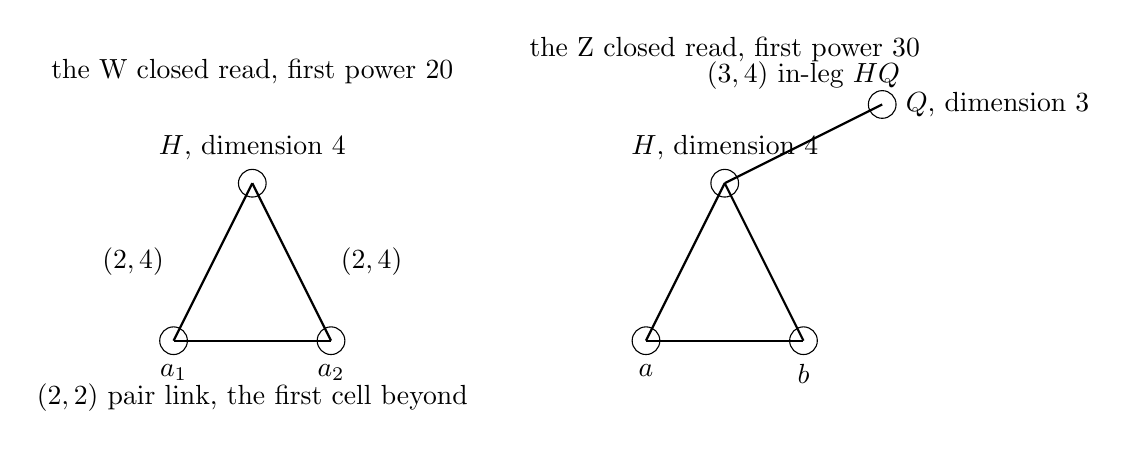
\begin{tikzpicture}[scale=1]
\filldraw[fill=white] (1,2) circle (5pt) node[above=5pt] {$H$, dimension 4};
\filldraw[fill=white] (0,0) circle (5pt) node[below=5pt] {$a_1$};
\filldraw[fill=white] (2,0) circle (5pt) node[below=5pt] {$a_2$};
\draw[thick] (1,2) -- (0,0); \draw[thick] (1,2) -- (2,0); \draw[thick] (0,0) -- (2,0);
\node at (1,0) [below=12pt] {$(2,2)$ pair link, the first cell beyond};
\node at (0,1) [left] {$(2,4)$}; \node at (2,1) [right] {$(2,4)$};
\node at (1,3) [above=4pt] {the W closed read, first power $20$};
\filldraw[fill=white] (7,2) circle (5pt) node[above=5pt] {$H$, dimension 4};
\filldraw[fill=white] (6,0) circle (5pt) node[below=5pt] {$a$};
\filldraw[fill=white] (8,0) circle (5pt) node[below=5pt] {$b$};
\filldraw[fill=white] (9,3) circle (5pt) node[right=5pt] {$Q$, dimension 3};
\draw[thick] (7,2) -- (6,0); \draw[thick] (7,2) -- (8,0); \draw[thick] (6,0) -- (8,0); \draw[thick] (7,2) -- (9,3);
\node at (8,3) [above=2pt] {$(3,4)$ in-leg $HQ$};
\node at (7,3) [above=12pt] {the Z closed read, first power $30$};
\end{tikzpicture}\caption{The two closed-genre reads: the W read over a (2,2) pair link and two (2,4) legs, and the Z read with its (3,4) in-leg, the two cells beyond the dock and the leg.}\end{figure}
\end{chproof}
\par\medskip\noindent{\itshape The carriers named, the next chapter is the chapter of their genre.}\label{narr:close:6-2}\par
\section{The instrument tables of this Part}\label{mod:VIII-L-the-instrument-tables-at-the-repository}
\chdesig{8-L}{}{VIII-L-the-instrument-tables-at-the-repository}{VIII-L-the-instrument-tables-at-the-repository}
\begin{chtable}[The instrument tables of this Part]\label{box:VIII-L-the-instrument-tables-at-the-repository:1}
This Part lists 13 instrument chapters, printed among the instruments at the end of this compendium as chapters~\ref{mod:VI-2a-2-4-genre-the-carrier-legs-and-the-neutral-lepton-ports} to~\ref{mod:VI-9-D543021-vcst-t1}, and the table beneath names each one with its key cells.
\end{chtable}
\chstanding{instrument}
\chdeps{Definitions 1.1 to 1.6}{no theorem beyond it at this release}
The listing moves no cell and states no result of its own. Each instrument stands at the repository as its chapter stood at the previous release of this compendium, and its tables are read there.
\begin{chbridge}
The tables listed here are instruments of this compendium, each listed under the title of its chapter.
\end{chbridge}
\begin{chproof}[instrument]
The listing in full. For each instrument chapter, printed among the instruments at the end of this compendium, the table gives its title, the result boxes it carries, the standing of each box with its citation, and the count of objects its certificate sentence names where it prints one.
{\small
\begin{longtable}{p{38mm}p{63mm}p{30mm}p{14mm}}
\hline
chapter & results & standing & objects \\
\hline
\endhead
The (2,4) genre: the carrier legs and the neutral-lepton ports & The (2,4) genre chapter & instrument & -- \\
The (2,4) genre: the carrier legs and the neutral-lepton ports & the text of the chapter & see its text & -- \\
The (2,4) genre: the carrier legs and the neutral-lepton ports & the text of the chapter & see its text & -- \\
The (2,4) genre: the carrier legs and the neutral-lepton ports & the text of the chapter & see its text & -- \\
The (2,4) genre: the carrier legs and the neutral-lepton ports & The open port and its conjugate end & theorem & 12 \\
The (2,4) genre: the carrier legs and the neutral-lepton ports & The weak angle as the ratio of the (2,3) and (2,4) dressings & open result & 519 \\
The charged and neutral currents & The currents chapter & instrument & -- \\
The charged and neutral currents & The neutral current as the Z read at the whole sinks & theorem & 36 \\
The charged and neutral currents & The charged current as the hub step at every sink & open result & 182 \\
The Fermi constant and the muon decay & The Fermi-constant chapter & instrument & -- \\
The Fermi constant and the muon decay & The Fermi constant as the W word office at low transfer & open result & 12 \\
The electroweak table & The electroweak table & instrument & -- \\
The electroweak table & The electroweak breaking as the stabilizer of the vacuum register & conditional theorem & 6 \\
\hline
\end{longtable}
}
The rule that produced it. Every chapter of this Part whose first standing beyond a placeholder reads instrument is printed among the instruments at the end of this compendium with its tables, and its key cells are the titles of its boxes, its standing lines and its certificate count, read from its text as it stood at the previous release.
No derivation stands in this chapter; the tables stand at the repository.
\emph{Check.} Every file listed was re-hashed at the repository and read the same as its recorded hash, and the listing was re-cut from the files by a second route.
Nothing stands open at this listing. At this release four results of this Part are re-graded at their chapters: the hub step as the weak interaction (the chapter 8-1), its open result closed as a conditional theorem at the decay path; the W and the Z (the chapter 8-2), the Z read re-posed at the route identity; the neutral lepton (the chapter 8-2b), the released body closed as a conditional theorem at the nested cross; beta decay (the chapter 8-8), closed as a theorem at the literal closure reading.
\end{chproof}
\label{chend:VIII-L-the-instrument-tables-at-the-repository}
\section{The neutral lepton: the hub unit with its legs open}\label{mod:VI-2b-neutral-lepton-the-hub-unit-with-its-legs-open}
\chdesig{8-2b}{6-2b}{VI-2b-neutral-lepton-the-hub-unit-with-its-legs-open}{VI-2b-neutral-lepton-the-hub-unit-with-its-legs-open}
\label{narr:open:6-2b}Theorem~162.1 reads the released body as one anatomy, the hub unit with its legs open, an open result, and Theorem~162.2 gives the census of the neutral sinks.
\begin{chconditional}[The released body as one anatomy]\label{box:VI-2b-neutral-lepton-the-hub-unit-with-its-legs-open:1}
Conditional on the results this theorem rests on at their own standing, as its derivation names them.
The released object of every generation is the cross nested at the depth one less, read at the order two through the hub: the body released at the second generation, four sites at the measure twenty-eight, is isomorphic at the labeled links to the hub assembly the nesting adds at the first depth by the least map of its sites, the body released at the third generation to the assembly added at the second depth by the corresponding map, every one of the three (2,4) hub links at the readability order two and the (2,2) pair at the order one at both objects at both generations, every link at the dressing of its genre at both spellings, and the body released at the first generation empty against the empty cross nested at the depth zero, the bare core nesting no cross; at the reading that gives the empty depth a body the first generation parts, both faces printed. The body released in every charged-lepton decay is thereby one anatomy, the junction assembly with its core in-leg struck, four sites at the measure twenty-eight, as the previous open result named it, and its identity with the nested cross of the next depth is the theorem; neutrality remains typed at the sinks of the saturation as two open qubit ports under the adopted definition, the two sets of the previous reading parting at the typed webs docked at charge zero, and whether the released body is of the Dirac or of the Majorana kind is a reading of the act and not an output of the construction; the deciding table is re-derived in Lean.
\end{chconditional}
\chstanding{conditional theorem, built at the nested cross}
\chdeps{Definitions 1.1 to 1.6, Theorem 152.1, Theorems 196.1 and 196.2 and Open results 245.1 and 245.2, Theorem 245.3, Open results 245.4 to 245.8 and Theorem 245.9}{Theorem 166.1 and Open results 166.2 and 166.3 and Theorem 254.1}
The box names the thing a decay releases, not a new kind of object but a piece of the decaying web, the hub with its leaf pair and its odd leg, left with two valences free where its core and its leaf stood. Neutral means two open qubit ports, and the box says that this typing is not the same as reading zero charge at every web.
\begin{chconditional}[The neutral sinks census]\label{box:VI-2b-neutral-lepton-the-hub-unit-with-its-legs-open:2}
Under the site-97 closure cut at wave four and the adopted definition of open at the ports, the lowest neutral sink of the census, at wave two, is a web of three sites and two qutrit-qubit links, among one hundred eighty-five neutral sinks counted wave by wave; the two neutral objects of the prior release stand among the sinks as one.
\end{chconditional}
\chstanding{conditional theorem, named at two ports}
\chdeps{Definitions 1.1 to 1.6, Theorem 152.1, Theorems 196.1 and 196.2 and Open results 245.1 and 245.2, Theorem 245.3, Open results 245.4 to 245.8 and Theorem 245.9}{Theorem 166.1 and Open results 166.2 and 166.3 and Theorem 254.1}
The second box is a count, among every sink the saturation reaches by wave four, those with exactly two open qubit ports are counted and the smallest is named as a web, with no name of the literature attached to it.
\begin{chbridge}
What this chapter calls the released body the literature calls the light neutral lepton released beside the charged one at its decay, and the hub unit with its legs open its neutral partner in the weak doublet. The correspondence is by name, and no mass, count or measured value enters this page.
\end{chbridge}
\begin{chproof}[exact]
The premises of the first box are the saturation with its waves and sinks of chapter 1-5, a theorem, the lepton ladder as hub assemblies of chapter 5-10, a theorem, and the unstable rows of chapter 8-3, an open result. The chain from the axiom to this chapter is eight chapters long. The exact part first. From the muon web, by the inverse hub step at its hub (the edge from the muon vertex to the electron vertex of the move graph of the first chapter of this Part), we obtain the released object, listed as a table here, the drawing means of this compendium admitting no picture.
\begin{center}\small
\begin{adjustbox}{max width=\linewidth}\begin{tabular}{llll}
\hline
site & dimension & link & genre \\
\hline
$H_2$ & 4 (the hub) & $H_2 b_1$ & (2,4) \\
$b_1$ & 2 (a leaf) & $H_2 b_2$ & (2,4) \\
$b_2$ & 2 (a leaf) & $H_2 b_3$ & (2,4) \\
$b_3$ & 2 (the odd leg) & $b_1 b_2$ & (2,2) \\
\hline
\end{tabular}\end{adjustbox}

The released body. The hub with its leaf pair and its odd leg, the in-link valence freed at the hub where the core stood and the pairing valence freed at the odd leg where the leaf stood.
\end{center}
From the four links, by the rank, we obtain the measure of the box,
\begin{equation}
28 = 2 \cdot 4 + 2 \cdot 4 + 2 \cdot 4 + 2 \cdot 2 ,
\end{equation}
and the same web is released at every one of the inverse edges of the move graph that release one. From the two free valences at the qubit ends, by the adopted definition of open, we obtain the typing of the box, two open qubit ports, neutral.

From the webs whose charge the construction establishes, by reading the established charge and the dock-free read side by side, we obtain the parting of the box, the established charge, typed at one hundred forty webs, reads zero at every one of them while the set of webs reading zero at the dock-free read holds more, so neutrality typed at the two ports and the dock-free read part at the typed webs docked at charge zero. At the readings beside, the cross-core pair released by the inverse hub step at the muon edge is two bodies at all nine pairs of readings and one body at none. The light neutral body as the Higgs link with its ports open parts from the charged partner at the structural reading. The Majorana-or-Dirac reading at the ports is a reading of the act and not an output of the literal clause. The baseline webs at the neutral sinks are unbuilt at the truncation, and one further reading takes the released object as one anatomy and not as the nesting of its generation.

The census part. From the sinks of the site-97 closure cut at wave four, by typing every sink at its open qubit ports, we obtain the four kinds, one sink beyond two ports, 5455 charged, 38700 dark with no open dock end, and the neutral sinks at two open dock ends,
\begin{equation}
185 = 1 + 6 + 178
\end{equation}
by wave two, three and four. By hub count they sort as 4, 4, 32, 56, 57, 20 and 12 at zero to six hubs. The smallest case. At wave two the one neutral sink is the web numbered 19, three sites $s_0$, $s_1$ of dimension 2 and $s_2$ of dimension 3 with the two links $s_0 s_2$ and $s_1 s_2$ of genre (2,3), its two open ports the docks at $s_0$ and $s_1$, reached from a root that is a pair ket by one attachment and one reversal. The nearest neutral sinks at one port fewer and at one port more are none. From the two neutral objects of the earlier result, by isomorphism against the sinks, we obtain one of them among the sinks (the triangle of dimensions 4, 2, 2 with two pendant ports, at one sink) and the other at none.

\emph{Check.} The eleven intermediate tables of the first box are cited at a note, the released object and its measure are taken from the result on the two neutral objects, which prints the same web at the muon edge, and the typing from the census result. Where a step of the first box is not carried by those two results it is stated and not derived here. What would have broken the census, the open definition replaced by the open dock ends or by the free valence at the qubit sites moves the port counts and leaves the lowest sink the same web. The twin closure at the web cap gives 62 neutral sinks with a different lowest sink at wave three. Each result was reproduced by an independent route, two engines at every capture byte for byte, its counter-tests at their pinned letters and its controls the same at both routes.
The mixing at the open ports is the matter of the mixing chapter of this Part.
\chcert{185}
\end{chproof}
\label{chend:VI-2b-neutral-lepton-the-hub-unit-with-its-legs-open}
\par\medskip\noindent{\itshape With the neutral lepton read, the next chapter pairs it with the charged one in the doublet.}\label{narr:close:6-2b}\par
\section{The doublets, handedness and parity violation}\label{mod:VI-3-doublets-handedness-and-parity-violation}
\chdesig{8-3}{6-3}{VI-3-doublets-handedness-and-parity-violation}{VI-3-doublets-handedness-and-parity-violation}
\label{narr:open:6-3}Theorem~163.1 gives the weak doublet at the internal ends of the leptons, Open result~163.2 the isospin sign as the dart charge minus half the weight, Theorem~163.3 the doublet count at the cross core, and Open result~163.4 the doublet as the set of sinks at every label and the sum at the set.
\begin{chconditional}[The weak doublet at the internal ends of the leptons]\label{box:VI-3-doublets-handedness-and-parity-violation:1}
Under the sixteen rows of chapter 4-1, the weights of chapter 4-2 and the open-end census of chapter 4-3, the weak doublet of a lepton is the one internal read at the odd leg of its junction: the one-act read that opens the odd-leg qubit copy is a doublet of the internal su(2) at the centre weight $n - 3$ and $6T_3 - 3$ with the two-ality $d = 1$, at the electron, the muon and the tau alike, every other internal read being closed under the join, closed at its dimension-four far end or washed at the (2,2) pair. The two charged-lepton rows of the sixteen are re-reached, the L row by the internal doublet read with the one-dock read beside it and the R row by the two-dock read, a singlet at $d = 0$; the two reads commute, the chirality from the dock link and the internal doublet from the hub leg varying independently.
\end{chconditional}
\chstanding{conditional theorem}
\chdeps{Definitions 1.1 to 1.6, Theorems 9.1 to 9.7 and Open result 9.8, Theorems 18.1 to 18.4 and Open results 18.5 and 18.6, Theorems 64.1 and 64.2, Theorems 65.1 and 65.2, Open results 66.1 to 66.3, Theorem 66.4 and Open result 66.5 and Open results 241.1 and 241.2, Theorems 241.3 and 241.4 and Open results 241.5 to 241.7}{Open results 72.1 to 72.3, Theorem 72.4 and Open result 72.5, Theorem 73.1 and Open results 73.2 and 73.3, Theorems 74.1 to 74.4 and Open result 74.5, Open result 163.4 and Theorems 200.1 to 200.3 and Open result 200.4}
Of all the one-act reads a lepton admits at its internal links, exactly one, at the odd leg of its junction, is a doublet, at all three charged leptons alike. The handedness comes from the dock, so chirality and isospin are carried by two reads that commute.
\begin{chwall}[The isospin sign as the dart charge minus half the weight]\label{box:VI-3-doublets-handedness-and-parity-violation:2}
The isospin component a lepton occupies, read as the dart charge, the charge of a directed edge, minus half the weight at the internal end, is an exact object at every body. On the one face the electron and the neutral body agree with the sixteen rows at the component, the sign and the weight; on the other face the muon and the tau part from them, the parting at the muon.
\end{chwall}
\chstanding{open result, built and not closed}
\chdeps{Definitions 1.1 to 1.6, Theorems 9.1 to 9.7 and Open result 9.8, Theorems 18.1 to 18.4 and Open results 18.5 and 18.6, Theorems 64.1 and 64.2, Theorems 65.1 and 65.2, Open results 66.1 to 66.3, Theorem 66.4 and Open result 66.5 and Open results 241.1 and 241.2, Theorems 241.3 and 241.4 and Open results 241.5 to 241.7}{Open results 72.1 to 72.3, Theorem 72.4 and Open result 72.5, Theorem 73.1 and Open results 73.2 and 73.3, Theorems 74.1 to 74.4 and Open result 74.5, Open result 163.4 and Theorems 200.1 to 200.3 and Open result 200.4}
The sign inside the doublet is an integer in sixths from two counts of the web, agreeing with the sixteen rows at the first generation and parting at the second and third.
\begin{chconditional}[The doublet count at the cross core]\label{box:VI-3-doublets-handedness-and-parity-violation:3}
Under the statistics from the odd-cycle sign, the doublet swap at the generic qubit read and the roster of bodies, the doublet count rule holds at the cross core of the three cross-core webs, where the depths read odd and the swap is met at the eighteen objects.
\end{chconditional}
\chstanding{conditional theorem}
\chdeps{Definitions 1.1 to 1.6, Theorems 9.1 to 9.7 and Open result 9.8, Theorems 18.1 to 18.4 and Open results 18.5 and 18.6, Theorems 64.1 and 64.2, Theorems 65.1 and 65.2, Open results 66.1 to 66.3, Theorem 66.4 and Open result 66.5 and Open results 241.1 and 241.2, Theorems 241.3 and 241.4 and Open results 241.5 to 241.7}{Open results 72.1 to 72.3, Theorem 72.4 and Open result 72.5, Theorem 73.1 and Open results 73.2 and 73.3, Theorems 74.1 to 74.4 and Open result 74.5, Open result 163.4 and Theorems 200.1 to 200.3 and Open result 200.4}
The third box counts doublets at the shared core of the three cross-core webs, the rule met at all eighteen objects.
\begin{chbridge}
What this chapter calls the internal doublet read the literature calls the weak isospin doublet of the left-handed leptons, the dock read its chirality and the component in sixths its third isospin component, the nearest objects. The correspondence is by name.
\end{chbridge}
\begin{chproof}[census]
The premises are the link and its six genres of chapter 1-2, the reads and the Born count of chapter 1-3 and the moves of chapter 1-4, definitions, and the sixteen rows, the weights and the open-end census of chapters 4-1 to 4-3, theorems and open results. The chain from the axiom to this chapter is seven chapters long. The set counted is the set of one-act reads at the internal links of the three lepton bodies, generated by opening each internal link at its qubit copy with the hub leg entered at its ket copy and the join kept. The property tested is whether the read is a doublet of the internal su(2). By kind the reads sort into the one doublet read per body, at the odd-leg copy of the junction, with the two-ality 1 and the weights $n - 3$ and $6T_3 - 3$, and the rest, closed under the join, closed at a dimension-four far end, or washed at the (2,2) pair. The smallest case. At the electron the one-dock read beside the doublet read carries the weight $n - 3$ equal to the row $6Y$, the dock count 1 the chirality L. The two-dock read is the singlet at $d = 0$, $6T_3 = 0$ and $n - 6$ by the exchange sign at the two dock ends, the row R. The two reads act on distinct links with disjoint open sets, so they commute, and the sixteen rows are re-reached at their ordinals, 16 of 16.

From the dart charge at the dock face and the half-weight at the internal end, by subtraction, the components at the four bodies are
\begin{equation}
-6 - (-3) = -3, \qquad 0 - (-3) = 3, \qquad -12 - (-3) = -9, \qquad -18 - 0 = -18 ,
\end{equation}
at the electron, the neutral body, the muon and the tau, every sign the odd-leg state, the electron and the neutral body agreeing with the sixteen rows and the muon and the tau parting. The doublet count rule is met at the cross core of the three cross-core webs at 18 of 18 objects, the depths reading odd there.

\emph{Check.} At the reading with the hub never entered no internal read is a doublet at any body, printed beside. The neutral body under the kept join carries no internal doublet at either reading. The counts of the closed and washed reads stand at the tables of the entry and are not re-listed here. Each result was reproduced by an independent route, two engines at every capture byte for byte, its counter-tests at their pinned letters and its controls the same at both routes.
The doublet content under the weights does not follow the dock count, and the component at the muon and the tau parts from the sixteen rows.
\chcert{16}
\end{chproof}
\label{chend:VI-3-doublets-handedness-and-parity-violation}
\subsection{The doublet as the set of sinks at every label}\label{mod:VI-3-D538842-w-dbcl}
\begin{chwall}[The doublet as the set of sinks at every label and the sum at the set]\label{box:VI-3-D538842-w-dbcl:1}
At every label of the representation census the set of stable webs, the sinks, at that label is a doublet set and the catalogued body lies inside it, but the sum over the set is nonzero at every label. On the one face a doublet member is found at every one of the three labels with the body inside its set; on the other face the four sums over the words the set reaches read 3, 189, minus 3 and 0 at every label where zero was asked, the first label without being the label one.
\end{chwall}
\chstanding{open result, built and not closed}
\chdeps{Definitions 1.1 to 1.6, Open results 66.1 to 66.3, Theorem 66.4 and Open result 66.5 and Theorem 163.1, Open result 163.2 and Theorem 163.3}{no theorem beyond it at this release}
The box re-reads the doublets of this chapter at the level of whole stable webs, the sinks of the saturation sorted by the number of their hubs, which the compendium reads as the generation, form three sets, each set contains doublet members and the cataloged lepton of that generation, and the anomaly-like sums that an earlier reading asked to vanish do not vanish over any of the three sets.
\begin{chbridge}
What this chapter calls the sink set at a label the literature calls the multiplet of a generation, and the doublet member its left-handed doublet, the nearest objects. The correspondence is by name.
\end{chbridge}
\begin{chproof}[finite computation]
The premises are the doublets of this chapter, a theorem, the representations from the open-end census of chapter 4-3, a theorem, and the saturation with its sinks of chapter 1-5, a theorem. The chain from the axiom to this result is eight chapters long. The procedure. The input is the union of 22302 saturated sinks and its 744 lepton-form sinks. The enumeration sorts them by hub count, the label of the generation,
\begin{equation}
744 = 48 + 156 + 231 + 300 + 9
\end{equation}
at zero, one, two, three and more hubs. The test at each sink is its typing at the dock rule, a doublet of color one, a weak singlet of color one, or a vanishing content. The aggregation is the four sums over the words the set reaches. The smallest instance is the set at the label one,
\begin{equation}
156 = 35 + 54 + 67 ,
\end{equation}
thirty-five doublet members (the first in the order of the material a proton sink at one dock), fifty-four weak singlets and sixty-seven at a vanishing content. The cataloged electron, located among them by isomorphism at two docks, lies inside the set as a weak singlet and inside the doublet subset not. At the labels two and three the doublet members are 60 of 231 and 129 of 300, the first a proton sink and a tau-row sink, and the cataloged bodies of those generations lie inside the doublet subset.

From the members at a label, by the words the set reaches at the adopted typing, two words at each label (89 of 156, 138 of 231 and 300 of 300 members at a word), and by the four sums with the weights 3 per open qubit end and minus 2 per open qutrit end, we obtain at every label the same four values, the linear sum, the cubic sum and the two mixed sums,
\begin{equation}
\ell = 3, \qquad c = 189, \qquad m_{2} = -3, \qquad m_{3} = 0 ,
\end{equation}
zero at 0 of 3 labels. Over the doublet members alone the sums read minus 3, minus 27, minus 3 and 0, and over the members with multiplicity 219, 10719, minus 105 and 0 at the label one, nonzero likewise. So the doublets clause holds, the sums clause fails, and the open result is named at the label one.

\emph{Check.} Reading the label by the attach-site count in place of the hub count sorts the sinks as 98, 488, 154, 2 and 2 and leaves the board labels present and the sums nonzero. The cataloged body is inside the doublet subset proper at two of the three labels. The result was reproduced by an independent route, two engines at every capture byte for byte, its counter-tests at their pinned letters and its controls the same at both routes.
The sum over the doublet set stays nonzero at every label.
\chcert{744}
\end{chproof}
\label{chend:VI-3-D538842-w-dbcl}
\par\medskip\noindent{\itshape The doublets read, the next chapter reads the two currents that run between their members.}\label{narr:close:6-3}\par
\section{The weak angle}\label{mod:VI-6-weak-angle}
\chdesig{8-6}{6-6}{VI-6-weak-angle}{VI-6-D539645-w-wbsq}
\label{narr:open:6-6}Theorem~164.1 reads the weak angle as the dock share, Open result~164.2 as the office of the W word, Open result~164.3 from the stabilizer weights, Open result~164.4 per family at the tau sink, and Theorem~164.5 as the ratio of offices at the Z body.
\begin{chconditional}[The weak angle as the dock share]\label{box:VI-6-weak-angle:1}
Under the results it rests on, the dock share is one structure at the W body, the Z body and their joined web: the two bodies, the roster W word and the roster Z word, are each a seeded sink at wave zero at both stop readings, five sites and four links at the genres qutrit-qubit twice and ququart-qubit twice, the measure twenty-eight, isomorphic by an explicit map, each with a total end set of eight ends and the dock ends of its two qutrit-qubit links; the dock share is a per-link quotient, additive over the links and unmoved by a shared site.
\end{chconditional}
\chstanding{conditional theorem}
\chdeps{Definitions 1.1 to 1.6, Theorems 185.1 to 185.12 and Theorems 197.1 to 197.4 and Open result 197.5}{Theorem 164.5, Chapter 8-6 and Theorem 255.1}
The box says that the quantity the compendium reads as the weak angle, the share of a body's ends that are dock ends, is the same structure whether read at the W, at the Z or at the two joined, because it is computed link by link and the two bodies are the same web.
\begin{chwall}[The weak angle as the office of the W word]\label{box:VI-6-weak-angle:2}
The count readings of the coupling read rule, met again from the pair ket at the qutrit-qubit read links of the W word and the Z word, are seventeen over thirty-six at the whole and fourteen over thirty-six at the cut, equal to the established cells at both words. On the one face the count faces are re-met from the pair ket and the office of the W word is the Born square of its first power; on the other face the step from the office of the W word to the square of the angle is refused at its first step, the third of five, the closed read, since the first power 28 over either unit is named the closed read by no established clause.
\end{chwall}
\chstanding{open result, built and not closed}
\chdeps{Definitions 1.1 to 1.6, Theorems 185.1 to 185.12 and Theorems 197.1 to 197.4 and Open result 197.5}{Theorem 164.5, Chapter 8-6 and Theorem 255.1}
The second box tries to derive the squared angle from the office rule applied to the W word, and finds the rule licenses only its first two steps there. The count face of the pair ket and the first power of the word are two different numbers and no clause makes one the other.
\begin{chwall}[The weak angle from the stabilizer weights]\label{box:VI-6-weak-angle:3}
The end-face figure of the angle from the stabiliser weights is three over eight at the dock reading and two over five at the hub reading, an exact rational; on the other face the established running rows carry that figure at no rung.
\end{chwall}
\chstanding{open result, built and not closed}
\chdeps{Definitions 1.1 to 1.6, Theorems 185.1 to 185.12 and Theorems 197.1 to 197.4 and Open result 197.5}{Theorem 164.5, Chapter 8-6 and Theorem 255.1}
The third box gives a figure for the angle from the norm ratio of two directions of the register, and finds it at no rung of the running.
\begin{chwall}[The weak angle per family at the tau sink]\label{box:VI-6-weak-angle:4}
The weak angle per family at the tau sink stands as an open result named at its second face: the three family shares read two thirds, one third and one half at the electron, the muon and the tau with the family average one half.
\end{chwall}
\chstanding{open result, built and not closed}
\chdeps{Definitions 1.1 to 1.6, Theorems 185.1 to 185.12 and Theorems 197.1 to 197.4 and Open result 197.5}{Theorem 164.5, Chapter 8-6 and Theorem 255.1}
The fourth box reads the share family by family. The tau share and the average equal the cell of the next section, the electron and the muon do not.
\begin{chbridge}
What this chapter calls the dock share, the count face and the office ratio the literature calls the squared sine of the weak mixing angle, each the nearest object. The correspondence is by name, and the value of the angle is displayed nowhere in this chapter.
\end{chbridge}
\begin{chproof}[finite computation]
The premises are the mass unit and the first power of chapter 8-1, a theorem, the three generations as attach sites of chapter 8-4, a theorem, and the W word of chapter 6-2, an open result. The chain from the axiom to this chapter is eight chapters long. The procedure of the second box, the input is the W word, five sites of dimensions 4, 2, 3, 2, 4 and four links, and the Z word, the same web. The enumeration lists the reads the read rule admits at end product at most 6, the two qutrit-qubit links at the middle site. The test poses the pair ket on the common support of dimension 2 and counts the 36 pair letters of the qutrit end and the qubit end by the amplitude of each. The aggregation is the count face. From the 36 pair letters, 17 nonzero at the whole and 14 at the cut, we obtain
\begin{equation}
\frac{17}{36}, \qquad \frac{14}{36} = \frac{7}{18}, \qquad \Bigl(\frac{17}{36}\Bigr)^{2} = \frac{289}{1296}, \qquad \Bigl(\frac{7}{18}\Bigr)^{2} = \frac{49}{324} ,
\end{equation}
with the sector sums one sixth, one twelfth, zero and three quarters at the weight sum 1, equal to the established cells of the two-read entry and the coupling-read entry at both words. From the first power of the W word, the rank 28 at the dressing 1, by the Born square over the unit 201 at the hub face and 67 at the dock face, we obtain the office
\begin{equation}
\Bigl(\frac{28}{201}\Bigr)^{2} = \frac{784}{40401}, \qquad \Bigl(\frac{28}{67}\Bigr)^{2} = \frac{784}{4489} ,
\end{equation}
equal to the office, support and Born tables of the office entry at both words. The five steps of the office rule, the body, the support, the closed read, the Born square and the unit, are licensed at 5 of 5 when the closed read is the first power and at 2 of 5 when it is the count face, the third step refuses, the parting of the box, with both objects printed,
\begin{equation}
\frac{289}{1296} \neq \frac{784}{40401}, \qquad \frac{49}{324} \neq \frac{784}{4489} .
\end{equation}

For the first box, from the two words as seeded sinks at wave zero at both stop readings, by listing their ends, we obtain eight ends at each and the dock ends of the two qutrit-qubit links. The dock share is the per-link quotient, additive over the links and unmoved by the shared site, one structure at the W, at the Z and at the joined web. The Z word is tied to the W word at 17 of 17 register cells, the difference zero and the ratio one at every one, the measure, the rank and the first power 28. At the qutrit-qubit genre the whole 36, the cut 24, the common-support register 16 and the two links. At the ququart-qubit genre the whole 64, the cut 45, the register 16 and the two links. The count faces and the offices. The register of the Z body is the Born count of the qutrit-qubit genre from its coherent sector counts at the basis gains,
\begin{equation}
319 = 79 \cdot 1 + 48 \cdot 2 + 42 \cdot 3 + 3 \cdot 6 .
\end{equation}
For the third box the end-face figure is the norm ratio of the third-component direction against the charge under the plain trace form on the register of the split at the matched scale, three over eight at the dock reading and two over five at the hub reading, unmoved under the composed map at every rung and carried by the running rows at none. For the fourth box the shares read two thirds, one third and one half with the average one half.

\emph{Check.} What would have broken the second result, the ququart-qubit legs give the count faces 22 over 64 and 19 over 64 and the closed-read genre of the carrier entry 4 over 16 and 3 over 16, neither the office. The Z word tried in place of the W word gives every cell the same. Each result was reproduced by an independent route, two engines at every capture byte for byte, its counter-tests at their pinned letters (four at the office rule) and its controls the same at both routes (ten there).
The step from the office of the W word to the square of the angle stays refused at its third step, and the figure from the stabilizer weights stands at no rung of the running, which is the matter of chapter 5-7.
\chcert{36}
\end{chproof}
\label{chend:VI-6-weak-angle}
\subsection{The weak angle as the ratio of offices at the Z body}\label{mod:VI-6-D539022-wazb-t1}
\begin{chconditional}[The weak angle as the ratio of offices at the Z body]\label{box:VI-6-D539022-wazb-t1:1}
Under the results it rests on, the office of the W word and the office of its two-line read are both defined at the register of the Z body, and their ratio is the exact rational one half, one cell at the Z body: equal at the Z-body register, at the hub unit and at the dock unit, the unit cancelling; equal at the three count-level forms of the weights; and equal at both orthogonal-sum readings.
\end{chconditional}
\chstanding{conditional theorem}
\chdeps{Definitions 1.1 to 1.6, Open results 159.1 and 159.2 and Theorem 164.1 and Open results 164.2 to 164.4}{no theorem beyond it at this release}
The box divides the Born square of the one-line read by the Born square of the two-line read at one register, the register the Z body reaches, and finds one half, the same number whichever unit, count-level weighting or orthogonal reading is chosen. The tau share and the family average of the chapter above equal it, the electron and muon shares do not.
\begin{chbridge}
What this chapter calls the ratio of the two offices the literature calls the squared cosine of the weak mixing angle, its complement the squared sine, and the Z body the Z boson, the first two the nearest objects and the last by name. The correspondence is by name, and no value of the angle is displayed here.
\end{chbridge}
\begin{chproof}[census]
The premises are the W and the Z of chapter 6-2, an open result, and the weak angle chapter above. The chain from the axiom to this result is nine chapters long. The exact part first. From the first power of the W word 28, re-met at five sources, and the register the Z body reaches, the Born count 319 of the qutrit-qubit genre, by the Born square, we obtain the office of the W word. From the orthogonal two-line sum $28\sqrt{2}$ at the count form, by the same square, the office of the Z read, and by division their ratio,
\begin{equation}
\frac{784}{101761}, \qquad \frac{1568}{101761}, \qquad \frac{784}{1568} = \frac{1}{2} ,
\end{equation}
with the complement one half, the inverse 2 and the square polarity three quarters beside. At the hub unit the two offices read 784 and 1568 over 40401 and at the dock unit over 4489, the ratio one half at every register.

The census part. The set counted is the grid of forms, readings and registers at which the two offices are defined, 99 cells of the office table. The property tested is whether the ratio equals the cell of the box, one half. By kind. At the three registers 3 of 3 equal. At the three count-level forms, the count, pair and sup-pair forms, 3 of 3. At the two orthogonal-sum readings 2 of 2. At the three forms beyond the count level the ratio parts, one seventeenth, one thirty-seventh and one tenth at the amplitude weights and one fifth, one seventh and one quarter at the Born weights, the first parting the sup-near form at one seventeenth. At the two amplitude-sum readings it parts, one quarter at the count-level forms. The smallest case is the count form at the orthogonal reading at the Z-body register, the display above. From the three family shares, by comparison, we obtain the tau share one half and the family average one half equal to the cell, the electron share two thirds and the muon share one third parting.

\emph{Check.} The Z body is the W word at 17 of 17 register cells and isomorphic to it at the identity map, so the two offices are defined at one register. The partings beyond the count level and at the amplitude readings are printed beside. The result was reproduced by an independent route, two engines at every capture byte for byte, its four counter-tests at their pinned letters and its twelve controls the same at both routes.
The comparison of the cell with the measured angle stands at the comparison table alone.
\chcert{99}
\end{chproof}
\label{chend:VI-6-D539022-wazb-t1}
\section{The weak angle as the office of the W word pair ket}\label{mod:VI-6-D539645-w-wbsq}
In the electroweak theory the weak mixing angle fixes the ratio of the W and the Z masses at the tree level and the relative strength of the neutral and the charged currents; its sine squared is the ratio of the squared couplings, a free parameter of the Standard Model fixed by measurement and not by the theory \cite{Glashow1961,Weinberg1967,Salam1968}. The weak angle is introduced at section~\ref{mod:VI-6-weak-angle}, the W and the Z at section~\ref{mod:VI-2-w-and-the-z-and-their-masses} and the body-alone office rule at section~\ref{mod:VIII-2-body-alone-office-rule}.
The count face of the pair ket at the (2,3) read link of the W word, 17 over 36 at the whole and 14 over 36 at the cut, agrees with the established values at 4 of 4 links of the word, the Z word tied at 4 of 4; but it is no first power of the body-alone rule read at the word, so the weak angle is not the office of the W-word pair ket at any of the three clauses posed.
The rule names the first power 28 at the word, from the measures 8, 6, 6 and 8 at the dressing one with nothing struck and the pair part 784 by the two-read identity; the dark set is the two (2,4) legs and the closure 10241 over 3645000 plus 98 over 50625 root 2 at the swapped weight of the (2,4) genre, the office 2857690241 over 3645000 plus 98 over 50625 root 2 agreeing with the W read and the W word result. At the register 36 of the read link the first power reads 7 over 9 against the count faces 17 over 36 and 7 over 18, and the office over the register squared is an element of the field with a root 2 part against the rational Born squares 289 over 1296 and 49 over 324; at the read link alone the first power is 6 and the office 36, parting likewise with the dark set empty there, at the two read links 12 and 144, and at the segment reading the word is carried at no read. The Born squares are exact values at both faces, and a grid of 72 readings meets at none.
The result is an open one, an open result: the stronger statement is not met at the whole face nor at the cut face, and the weaker statement is named; no comparison with observation is made here.
What stays open is whether the Born square at the word is an output of the body-alone rule, which no result settles at this stage; the weak angle at the one value of the Z body (section~\ref{mod:VI-6-D539022-wazb-t1}) and the Z read of the W word (section~\ref{mod:VI-2-w-and-the-z-and-their-masses}) stand beside at their own sections.
\par\medskip\noindent{\itshape The angle read, the next chapter reads the mixing between the generations.}\label{narr:close:6-6}\par
\section{Mixing, the washed overlap and the CKM block}\label{mod:VI-7-mixing-the-washed-overlap-and-the-ckm-block}
\chdesig{8-7}{6-7}{VI-7-mixing-the-washed-overlap-and-the-ckm-block}{VI-7-D543182-w-mxog}
\label{narr:open:6-7}Theorem~166.1 reads mixing as the overlap of the corner frame with the depth eigenbasis, Open result~166.2 as the corner-frame overlap through the W, Open result~166.3 the mixing phase at the four-cycle and the dock weights, Open result~166.4 the mixing as the sink-basis overlap, Open result~166.5 as the washed overlap of the arm reads, and Open result~166.6 the quark mixing block at the read sites.
\begin{chconditional}[Mixing as the overlap of the corner frame with the depth eigenbasis]\label{box:VI-7-mixing-the-washed-overlap-and-the-ckm-block:1}
If the generation label is the depth momentum, and under the rung reading of the polar-unitary entry and the open results it rests on, the rung basis of the three families is the eigenbasis of the depth step and the mixing is the overlap of the corner frame, an eigenbasis at a corner of a lattice cell, with it: the depth-step operator is factored by the Chinese remainder map into a qubit share and a qutrit share, the three characters of the qutrit share are the eigenvectors of the unit rung shift, and the overlap of the corner basis with that eigenbasis is unitary by construction at every admitted cell at both corner-basis readings, a permutation at none, with every squared modulus one third, the order-three Fourier matrix at every admitted frame, its phase a third of a turn or two thirds at every quartet and a half turn at none.
\end{chconditional}
\chstanding{conditional theorem}
\chdeps{Definitions 1.1 to 1.6, Theorems 162.1 and 162.2 and Theorems 197.1 to 197.4 and Open result 197.5}{Theorem 27.1, Open result 166.4, Open result 166.5, Open result 166.6, Chapter 8-7, Open result 168.1, Open result 169.1 and Theorem 254.1}
The box identifies the mixing with a change of basis, one basis is the corner frame a lepton web carries at its dark triangle, the other the eigenbasis of the step that moves a body one rung up its ladder. The matrix between them is the discrete Fourier transform of order three, every entry of squared modulus one third.
\begin{chwall}[Mixing as the corner-frame overlap through the W]\label{box:VI-7-mixing-the-washed-overlap-and-the-ckm-block:2}
The overlap of the corner frame with the rung basis read through the W is not unitary at the primary reading. On the one face the lepton overlap through the W at the hub face is defined at all nine pairs and the quark overlap at the dock face at six of nine; on the other face the first pair at which the quark overlap is undefined is the up-type first-generation element against its down-type partner, returning nothing through its dock, and the first row not summing to one is the electron row, the rows and columns summing to one at none of the six.
\end{chwall}
\chstanding{open result, built and not closed}
\chdeps{Definitions 1.1 to 1.6, Theorems 162.1 and 162.2 and Theorems 197.1 to 197.4 and Open result 197.5}{Theorem 27.1, Open result 166.4, Open result 166.5, Open result 166.6, Chapter 8-7, Open result 168.1, Open result 169.1 and Theorem 254.1}
The second box reads the same overlap not as a change of basis but through the W, as a two-point read between a flavor web and a mass web joined at the hub. The resulting matrix of squared moduli is defined but is not unitary, and the open result stands at the first row whose entries do not sum to one.
\begin{chwall}[The mixing phase at the four-cycle and the dock weights]\label{box:VI-7-mixing-the-washed-overlap-and-the-ckm-block:3}
The phase read at the four-cycle and the dock weights meets the measured entry at no reading.
\end{chwall}
\chstanding{open result, built and not closed}
\chdeps{Definitions 1.1 to 1.6, Theorems 162.1 and 162.2 and Theorems 197.1 to 197.4 and Open result 197.5}{Theorem 27.1, Open result 166.4, Open result 166.5, Open result 166.6, Chapter 8-7, Open result 168.1, Open result 169.1 and Theorem 254.1}
The third box reads a phase off the four-cycle of the joined web and the dock weights and finds it at no reading equal to the entry the construction carries.
\begin{chbridge}
What this chapter calls the overlap of the corner frame with the depth eigenbasis the literature calls the lepton mixing matrix, and the overlap of the quark arm basis the quark mixing matrix of Cabibbo, Kobayashi and Maskawa, the nearest objects. The correspondence is by name, and no angle, phase or figure is displayed at this page.
\end{chbridge}
\begin{chproof}[finite computation]
The premises are the neutral lepton of chapter 6-2b, an open result, and the three generations as attach sites of chapter 8-4, a theorem, with the framework. The chain from the axiom to this chapter is nine chapters long. The procedure of the second box, the inputs are the three lepton corner frames, the dark triangle of each lepton web with the corner links beyond it (the frames of one, two and three hub legs), the six quark arm signatures and the mass-ordered rung basis of every family, the leptons at the chain sums 201, 963 and 3969, the up-type quarks at 6, 120 and 684 and the down-type at 138, 720 and 3132. The enumeration joins every flavor web to every mass web of its family at the hub face for the leptons and at the dock face for the quarks, nine joined webs each (the first, the electron against itself, at 21 sites, 24 links and 48 arrows). The test is the W read through the joined web, a record passed from the flavor corner to the mass corner, with the determinant of one minus the arrow operator nonzero at 18 of 18 webs. The aggregation is the squared modulus, the cross sum squared over the absolute product of the two diagonal sums. The smallest instance is the electron against itself at the hub face, the four sums
\begin{equation} \adjustbox{max width=\dimexpr\linewidth-3em\relax}{$\displaystyle \begin{gathered} S_{fm} = S_{mf} = \frac{-39145204800 - 3929277600\sqrt{3}}{3185076713521}, \\ S_{ff} = S_{mm} = \frac{98631536274 + 649317125442\sqrt{3}}{3185076713521}, \end{gathered}$} \end{equation}
and the squared modulus, the cross sum squared over the absolute product of the two diagonal sums, an exact element of the ring whose numerator and denominator run to nineteen digits and stand at the table of the entry.
\begin{figure}[htbp]\centering
{\scriptsize\setlength{\tabcolsep}{3pt}\begin{adjustbox}{max width=\linewidth}\begin{tabular}{|p{30mm}|p{28mm}|p{28mm}|p{28mm}|p{28mm}|}
\hline
the first letter, its orientation and its conjugation; the second letter across & \textbf{Z} & \textbf{X} & \textbf{XZ} & \textbf{XZ2} \\ \hline
\textbf{Z} \newline even, self & the recorded sign \textbf{zero} \newline the plain reading zero, the conjugate reading zero \newline the square 0 \newline the block equal, the orientation reading equal & the recorded sign \textbf{plus} \newline the plain reading plus, the conjugate reading plus \newline the square 1/108 \newline the block equal, the orientation reading equal & the recorded sign \textbf{plus} \newline the plain reading plus, the conjugate reading plus \newline the square 1/108 \newline the block equal, the orientation reading equal & the recorded sign \textbf{plus} \newline the plain reading plus, the conjugate reading plus \newline the square 1/108 \newline the block equal, the orientation reading equal \\ \hline
\textbf{X} \newline odd, self & the recorded sign \textbf{plus} \newline the plain reading minus, the conjugate reading plus \newline the square 1/108 \newline the block equal, the orientation reading equal & the recorded sign \textbf{zero} \newline the plain reading zero, the conjugate reading zero \newline the square 0 \newline the block equal, the orientation reading equal & the recorded sign \textbf{plus} \newline the plain reading minus, the conjugate reading plus \newline the square 1/108 \newline the block equal, the orientation reading equal & the recorded sign \textbf{minus} \newline the plain reading plus, the conjugate reading minus \newline the square 1/108 \newline the block equal, the orientation reading equal \\ \hline
\textbf{XZ} \newline odd, the pair with XZ2 & the recorded sign \textbf{plus} \newline the plain reading minus, the conjugate reading plus \newline the square 1/108 \newline the block equal, the orientation reading equal & the recorded sign \textbf{plus} \newline the plain reading plus, the conjugate reading plus \newline the square 1/108 \newline the block equal, the orientation reading equal & the recorded sign \textbf{minus} \newline the plain reading zero, the conjugate reading minus \newline the square 1/108 \newline the block equal, the orientation reading equal & the recorded sign \textbf{zero} \newline the plain reading minus, the conjugate reading zero \newline the square 0 \newline the block equal, the orientation reading equal \\ \hline
\textbf{XZ2} \newline odd, the pair with XZ & the recorded sign \textbf{plus} \newline the plain reading minus, the conjugate reading plus \newline the square 1/108 \newline the block equal, the orientation reading equal & the recorded sign \textbf{minus} \newline the plain reading minus, the conjugate reading minus \newline the square 1/108 \newline the block equal, the orientation reading equal & the recorded sign \textbf{zero} \newline the plain reading plus, the conjugate reading zero \newline the square 0 \newline the block equal, the orientation reading equal & the recorded sign \textbf{plus} \newline the plain reading zero, the conjugate reading plus \newline the square 1/108 \newline the block equal, the orientation reading equal \\ \hline
\end{tabular}\end{adjustbox}}
\par\smallskip
{\footnotesize the census of the recorded signs: plus 9, minus 3, zero 4; the conjugate reading equal the recorded sign at 16 of 16 pairings; the conjugate Gram equal the recorded mixing block at 16 of 16 pairings and 128 of 128 cells; the recorded reading (the orientation sign of the first letter multiplied by the plain-reading sign at the partner pairing) equal at 16 of 16; the reading beside (the orientation class alone at the same pairing) equal at 10 of 16 with its first parting XZ.X}
\caption{The mixing Gram at the sixteen pairings of the four core letters Z, X, XZ and XZ2, the recorded blocks at one hub letter. At every pairing the conjugate Gram, the overlap Gram read with the first pairing as the recorded bra, equals the recorded mixing block at every cell, and the sign of its sign cell is the end-swap orientation of the first letter: the recorded sign is the orientation sign of the first letter multiplied by the plain-reading sign at the partner pairing, equal at sixteen of sixteen with the first parting none, the orientation classes Z even, X odd, XZ odd, XZ2 odd and the conjugation classes Z self, X self, XZ the pair with XZ2, XZ2 the pair with XZ (the sign cell is the Jarlskog invariant of the literature and the blocks its CKM block, by name).}\label{fig:mixing-gram}
\end{figure}

From the nine lepton pairs the same steps define the lepton matrix at 9 of 9 pairs. From the nine quark pairs the quark matrix is defined at 6 of 9, undefined first at the up-type first-generation element against its down-type partner, whose diagonal sum is zero because it returns nothing through its dock. The rows and columns of the lepton matrix sum to one at 0 of 6, the first row off the electron row, so the overlap through the W is not unitary, the parting of the second box. For the first box, from the depth-step operator at every admitted cell, by the Chinese remainder factoring into a qubit share and a qutrit share and by the three characters of the qutrit share, we obtain the eigenbasis of the unit rung shift. From the corner basis against it, by the inner products, we obtain the order-three Fourier matrix with the squared moduli
\begin{equation}
\frac{1}{3}
\end{equation}
at every entry, unitary at every admitted cell at both corner-basis readings and a permutation at none, its phase a third or two thirds of a turn at every quartet. The moduli one third and one half of the naming entry stand at the quartet object. For the third box the phase at the four-cycle and the dock weights is read at its readings and parts from the carried entry at every one.

\emph{Check.} At the readings beside, the three pairwise sector-normalized transforms between the corner frames of the charged-lepton dark triangle are unitary at none of the three. The normalization at the read and the neutral body at the second-order dark read are readings whose entries stand at the reference list. The count face at the joined web and the overlap at the open ports of the hub pair, defined at one of three generations, are readings tried and parted at their named steps. Each result was reproduced by an independent route, two engines at every capture byte for byte, its counter-tests at their pinned letters and its controls the same at both routes.
The overlap through the W stays not unitary at the primary reading, and the phase at the four-cycle and the dock weights parts from the carried entry at its second reading.
\chcert{18}
\end{chproof}
\label{chend:VI-7-mixing-the-washed-overlap-and-the-ckm-block}
\subsection{The mixing as the sink-basis overlap}\label{mod:VI-7-D536241-w-mxso}
\begin{chwall}[The mixing as the sink-basis overlap]\label{box:VI-7-D536241-w-mxso:1}
With the arm bases of the catalogued sinks taken as the reads of their shared sites, one direction per pair, at every admitted cap letter, the quark mixing overlap at the junction register is unitary at all 16 letter pairs, with its overlap-cycle phases inside the phase group of the (3,3) genre at all 108 and its Jarlskog invariant nonzero at 12 of the 16 pairs, but the lepton mixing overlap at the hub register is not unitary at the catalogued sinks. On the one face the quark form is a unitary on three arms with the largest Jarlskog square one over 108; on the other face the lepton form is a frame of three rows against the dark-end count, square at none of the 389 seeded sinks, the parting named with both cells.
\end{chwall}
\chstanding{open result, built and not closed}
\chdeps{Definitions 1.1 to 1.6 and Theorem 166.1 and Open results 166.2 and 166.3}{no theorem beyond it at this release}
The box builds a mixing matrix from the stable webs themselves, at the junction of the proton and the neutron the three arms give a basis each, and the overlap of the two bases at every admitted letter is unitary with a nonzero phase invariant. At the hub of a lepton web the same construction gives a rectangular frame, not a square matrix, and the open result stands there.
\begin{chbridge}
What this chapter calls the quark overlap at the junction register the literature calls the quark mixing matrix of Cabibbo, Kobayashi and Maskawa, its overlap-cycle phase the invariant phase and its Jarlskog cell the Jarlskog determinant, the nearest objects. The correspondence is by name, and the comparison with the measured entries is made at the comparison table alone.
\end{chbridge}
\begin{chproof}[finite computation]
The premises are the mixing chapter above and the framework. The chain from the axiom to this result is ten chapters long. The procedure. The inputs are the cap bases of every register, the eigenbases of the admitted letters ($Z$, $X$, $XZ$ at the qubit end. $Z$, $X$, $XZ$, $XZ^{2}$ at the qutrit end. Five letters at the ququart end), rays on the power basis of the twenty-fourth root of unity at integral norms, 12 of 12 re-met ray by ray, and the nucleon sinks, the proton at the bound-respecting seed (8 sites, 9 links, the measure 81) and the neutron. The enumeration forms, at every ordered pair of the four qutrit letters, the overlap of the proton read transported along the three-link joined path against the neutron read, sixteen matrices of three rows by three columns, and at the hub register of each lepton web the overlap of the attach-site read against the hub read, one column per dark end. The test is unitarity, with the alternating four-cycle phases and the Jarlskog of each. The aggregation is the count of unitary pairs. The smallest instance is the letter $Z$ against itself, whose Born squares are the identity, and the letter $Z$ against $X$, whose Born squares are flat,
\begin{equation}
\begin{pmatrix} 1 & 0 & 0 \\ 0 & 1 & 0 \\ 0 & 0 & 1 \end{pmatrix}, \qquad \begin{pmatrix} 1/3 & 1/3 & 1/3 \\ 1/3 & 1/3 & 1/3 \\ 1/3 & 1/3 & 1/3 \end{pmatrix},
\end{equation}
the rows and columns summing to one at both, the first with every four-cycle trivial and the second with nine nonzero cycles at the cube-root phases and the Jarlskog square
\begin{equation}
J^{2} = \frac{1}{108} .
\end{equation}

From the sixteen quark matrices, by the test, we obtain unitary at 16 of 16, the phases inside the group of the (3,3) genre at 108 of 108 cycles, the cycles nontrivial at 12 of 16 letter pairs (trivial at the four pairs at which the conjugate of the proton letter is the neutron letter, $Z$ against $Z$, $X$ against $X$, $XZ$ against $XZ^{2}$ and $XZ^{2}$ against $XZ$) and the Jarlskog nonzero at 12 of 16, the largest square one over 108. From the lepton webs, by the same construction at the hub register, the hub reading one direction per dark end, four per hub assembly, against the three directions of the attach-site read, we obtain frames of shape three by four at the electron, three by eight at the muon and three by twelve at the tau, square at 0 of 389 seeded sinks, with the overlap-cycle phases inside the (3,4) group at 126 of 306. The four-cycle at the dock register is trivial at 9 of 9 letter pairs, the four-cycle root an eigenvalue and no Jarlskog at dimension two, so the phase of the mixing lives at the junction and not at the dock.

\emph{Check.} At the plain identification of the far end in place of the transported conjugate the Born squares are equal at every pair, as pinned. The overlaps stand as 45 printed structures with every entry an exact element on the power basis. The result was reproduced by an independent route, two engines at every capture byte for byte, its counter-tests at their pinned letters and its controls the same at both routes.
The lepton mixing overlap stays a frame of three rows against the dark-end count at every cataloged sink.
\chcert{389}
\end{chproof}
\label{chend:VI-7-D536241-w-mxso}
\subsection{The mixing as the washed overlap of the arm reads}\label{mod:VI-7-D538551-w-mxws}
\begin{chwall}[The mixing as the washed overlap of the arm reads]\label{box:VI-7-D538551-w-mxws:1}
The mixing is the washed overlap of the arm reads: at the shared qudit the known wash gives the amplitude zero and the Born share flat at one over the dimension, and the washed quark overlap is unitary at all sixteen blocks with a nonzero Jarlskog cell at twelve of the sixteen. On the one face the washed quark overlap is unitary at 16 of 16 letter pairs at the group of the construction and at the monomial group beside, its washed phases inside the (3,3) group at 108 of 108; on the other face the washed lepton overlap is unitary at 0 of 20 and a unitary on three at 0 of 20, its phases inside at 250 of 338, the parting named with both cells.
\end{chwall}
\chstanding{open result, built and not closed}
\chdeps{Definitions 1.1 to 1.6, Theorem 42.1 and Theorem 166.1 and Open results 166.2 and 166.3}{Open result 166.6}
The box applies the wash, the average over the matchings the definitions leave free at the qudit the two reads share, to the overlaps of the section above, every amplitude is averaged to zero and every Born square to the flat value, the quark overlap stays unitary and keeps its phase invariant, and the lepton overlap stays short of unitary.
\begin{chbridge}
What this chapter calls the known wash at the shared qudit the literature calls the twirl, the group average over the unfixed identifications, an exact correspondence. The correspondence is by name, and no mixing element is displayed here.
\end{chbridge}
\begin{chproof}[census]
The premises are the measurement as the wash at one act of chapter 2-4, a definition, the mixing chapter above and the sink-basis overlap beside. The chain from the axiom to this result is ten chapters long. The set counted is the set of alternating four-cycles of every overlap of the sink-basis result, 1539 cycles across the quark form, the lepton form and the dock form at every letter pair, and the property tested is whether the washed cycle invariant is a root inside the phase group of its genre. Beside it every washed overlap is tested for unitarity. The wash is the group average over the identification group of the apparatus-inertness entry at the shared qudit, the Weyl-Heisenberg group of the construction at the orders
\begin{equation}
8, \qquad 27, \qquad 64
\end{equation}
at the dimensions 2, 3 and 4 with its central phases, the monomial group at 32, 384 and 6144 beside. As a channel on the state of the shared end it is trace-preserving, unital and idempotent, its kernel the zero matrix at 6 of 6 and the twirl of every matrix unit the flat unit. The smallest case is the quark form at the junction register, dimension 3, at the letter $Z$ against $Z$. The group of order 27 enumerated as 9 elements with their central phases, six terms killed and three surviving per entry, the washed amplitude zero at every entry and the washed Born squares
\begin{equation}
\frac{1}{3}
\end{equation}
at every entry, flat, the row and column sums one. By kind the washed quark overlap is unitary at 16 of 16 letter pairs at the group of the construction and 16 of 16 at the monomial group, its washed moduli squared one third at every entry, its washed phases roots inside the (3,3) group at 108 of 108 cycles, nontrivial at 12 of 16 pairs and its washed Jarlskog nonzero at 12 of 16. The washed lepton overlap is unitary at 0 of 20 and a unitary on three at 0 of 20, its phases inside the group at 250 of 338. The dock form at dimension two carries no Jarlskog.

The washed row Gram matrix equals the unwashed at every matrix and the washed column Gram the unwashed at every square matrix, so the unitarity letters of the section above are unmoved by the wash. The per-cycle invariants, phases and Jarlskog cells are equal at the two computations at 1539 of 1539 cycles.

\emph{Check.} One census, the signs of the Jarlskog at eleven lepton letter pairs carrying cycles that are no roots, was counted by one route and not by the other, the per-cycle invariants equal at every cycle and the eleven censuses equal at the root-only grammar at a third route. No cell moved. The result was reproduced by an independent route, two engines at every capture byte for byte, its four counter-tests at their pinned letters and its controls the same at both routes.
The lepton mixing as the three-site block with its dark-end column is a result placed at no chapter here.
\chcert{1539}
\end{chproof}
\label{chend:VI-7-D538551-w-mxws}
\subsection{The quark mixing block at the read sites}\label{mod:VI-7-D538947-w-ckmb}
\begin{chwall}[The quark mixing block at the read sites]\label{box:VI-7-D538947-w-ckmb:1}
The washed quark overlap, read as the three-by-three block at the read sites, with the rows the three arms of the proton star and the columns the three arms of the neutron star, is unitary on three at all 16 letter pairs, with a one-valued Jarlskog cell of square one over 108 at the checkerboard at 12 of the 16 blocks. On the one face every block is unitary on three with its Jarlskog an exact cell; on the other face the Jarlskog is nonzero with the checkerboard at 10 of the 12 mixing pairs and zero at 2 of the 4 identity pairs, so the same-letter sorting parts at its first pair, named with both cells.
\end{chwall}
\chstanding{open result, built and not closed}
\chdeps{Definitions 1.1 to 1.6, Theorem 166.1 and Open results 166.2 and 166.3 and Open result 166.5}{no theorem beyond it at this release}
The box reads the washed overlap of the section above as a square block labeled by the arms of the two nucleon stars, which is the shape the literature's quark mixing matrix has. The block is unitary at every letter pair and carries one phase invariant, and the open result is that the invariant does not vanish exactly at the pairs of equal letters and only there.
\begin{chbridge}
What this chapter calls the block at the read sites the literature calls the quark mixing matrix, its row and column labels the up-type and down-type quarks of the two nucleons, and its Jarlskog cell the Jarlskog invariant, the nearest objects. The correspondence is by name, and no element of the block is displayed here.
\end{chbridge}
\begin{chproof}[exact]
The premises are the mixing chapter above and the washed overlap beside. The chain from the axiom to this result is eleven chapters long. The object is listed as a table here, the drawing means of this compendium admitting no picture, the block at the read sites,
\begin{center}\small
\begin{adjustbox}{max width=\linewidth}\begin{tabular}{lccc}
\hline
 & neutron arm $Q_1$ (up) & neutron arm $Q_2$ (down) & neutron arm $Q_3$ (down) \\
\hline
proton arm $Q_1$ (up) & $1/3$ & $1/3$ & $1/3$ \\
proton arm $Q_2$ (up) & $1/3$ & $1/3$ & $1/3$ \\
proton arm $Q_3$ (down) & $1/3$ & $1/3$ & $1/3$ \\
\hline
\end{tabular}\end{adjustbox}

The washed Born squares of the block at every one of the sixteen letter pairs, flat at one third, doubly stochastic.
\end{center}
From the washed quark overlap at the junction register, by reading it at the three arms of the proton star against the three arms of the neutron star at every ordered pair of the admitted letters $Z$, $X$, $XZ$ and $XZ^{2}$, four identity pairs and twelve mixing pairs, and at both identification groups, we obtain 32 blocks with the washed amplitude zero at every entry and the washed Born squares the flat matrix of the table at 16 of 16 pairs of the group of the construction, the row and column sums
\begin{equation}
\frac{1}{3} + \frac{1}{3} + \frac{1}{3} = 1 .
\end{equation}
From the washed Gram matrices of the rows and of the columns, both the identity at every block, we obtain the block unitary on three at 16 of 16 at the group of the construction and 16 of 16 at the monomial group, a frame at 0 of 16. From the nine alternating four-cycles of every block, by the washed cycle product and its imaginary part, we obtain the Jarlskog one-valued at 16 of 16 blocks, zero at the identity pairs of the letters $Z$ and $X$ and, at the mixing pair $Z$ against $X$, the exact cell
\begin{equation}
J = \frac{\sqrt{3}}{18}, \qquad J^{2} = \frac{1}{108},
\end{equation}
the signs of the nine cycles five plus and four minus, the checkerboard of a unitary on three. The same square stands at every mixing pair with a nonzero cell.

From the sixteen pairs, by sorting the Jarlskog by the pair kind, we obtain the cell nonzero with the checkerboard at 10 of the 12 mixing pairs and zero at 2 of the 4 identity pairs, so the sorting by equal letters parts at its first pair, the parting of the box. The arms of the two stars at the roster entry equal the row and column labels at 16 of 16 pairs, and the squares of the cycles re-met the recorded cycles at every block of both groups.

\emph{Check.} The identity letters of the washed Gram matrices recomputed equal the recorded table at every block, and the Jarlskog recomputed in the ring equals the recorded square at every cycle. The result was reproduced by an independent route, two engines at every capture byte for byte, its four counter-tests at their pinned letters and its twelve controls the same at both routes.
The same-letter sorting parts at its first pair, and the lepton block at the three sites with its dark-end column is placed at no chapter here.
\end{chproof}
\label{chend:VI-7-D538947-w-ckmb}
\section{Lepton mixing as the three-site block with the dark-end column}\label{mod:VI-7-D539152-w-lmde}
The lepton mixing block is a unitary three-by-three matrix whose squared moduli are the transition weights between the flavour and the mass states of the neutral partners; every row and every column of the squared moduli sums to one, and a block of squared moduli with a row sum below one marks a state outside the three, a further column \cite{Pontecorvo1958,Maki1962}. The mixing with the washed overlap is introduced at section~\ref{mod:VI-7-mixing-the-washed-overlap-and-the-ckm-block} and the neutral lepton as the hub unit with its legs open at section~\ref{mod:VI-2b-neutral-lepton-the-hub-unit-with-its-legs-open}.
The three-by-three block of the washed lepton overlap at the three read sites, with the dark end as a fourth column, is cut at every one of the six hub assemblies of the standard lepton webs and every one of the 20 letter pairs beyond the known wash at the shared hub qudit: its Born block is flat at one quarter with the row sums three quarters, and its row Gram and its column Gram are each three quarters of the identity, so the block is a scaled unitary at the read share three quarters at 20 of 20 and a unitary at the base criterion at 0 of 20, the dark-end column carrying the remaining quarter and completing the frame at 20 of 20.
The washed block phases fall inside the phase group of the (3,3) genre at 125 of 169 with the cycles exact at 10 of 20, and the two groups do not agree at their summaries. The scaled-unitary reading, the unread-end reading, unitary at 4 of 20 with the phases inside at 57 of 171, and the unwashed reading, unitary at 4 of 20, each stand at the second face. The first parting is the first assembly, the electron hub at the letter pair Z against Z with the dark-end column at the third leg, where the block is not unitary at the base criterion though its Gram scalar is three quarters; the second value named is the first washed block phase outside the phase group. Two independent implementations agree at every value and the runs are byte-identical.
The result is an open one, an open result: the stronger statement, a unitary block on three at the base criterion, is not met, and the weaker statement, a scaled unitary completed by the dark-end column, is named with both values; no comparison with observation enters its grade.
What stays open is a reading at which the block is unitary on three, found at none; the unwashed block at the open ports (section~\ref{mod:V-10-D539519-w-tflb}) stands beside at its own open question.
\section{The mixing blocks at the (3,4) legs}\label{mod:VI-7-D541437-w-mxtf}
\begin{chwall}[The mixing blocks at the (3,4) legs]\label{box:VI-7-D541437-w-mxtf:1}
This result is conditional on the results it rests on, the open results among them consumed at their tables at their grades, the composition riding the lowest grade in its chain, and on the readings of its source disclosed at its register. The mixing blocks at the (3,4) legs: at every one of the sixteen in-legs of the roster and the twenty letter pairs, the block of the hub read transported down the (3,4) in-leg against the leg basis, washed at the shared qutrit, has its read sites named by the leg at four of twenty pairs, is unitary on three at four of twenty and meets its kind at the conjugate sorting at four of twenty, the Jarlskog one cell at eleven of twenty with the squares $1/108$, $16/2187$, $4/2187$, $4/729$ and $8/2187$ and surds at ten, at the hub letter Z alone the first face with the squares $1/108$; the quark cell $1/108$ is re-met with the conjugate sorting and the zero of the unwashed block re-met; so the face read is the second at the first parting, the first pair in the frozen order, the core letter Z against the hub letter X, at every in-leg of the roster, first at the electron in-leg $HA$ with the (2,4) legs $a_{1}$, $a_{2}$ and $a_{3}$: the hub read transported down the in-leg has four nonzero members of four with the norms three quarters each and no member zero, so the three read sites are not named by the leg and the block needs a (2,4) leg cell, the base column naming the end $a_{3}$; the block at that cut is not unitary on three, the pair kind mixing is not met and the Jarlskog squares $4/729$ are one-valued without the checkerboard; the second cell, the hub letter Z alone, meets the first face at four of four with the squares $1/108$.
The first face, the blocks functions of the (3,4) leg cells alone with the conjugate sorting re-met at every pair, reads no at the face cell; the second face, a block needing a (2,4) leg cell with the first named with both cells, reads yes at the pair Z against X at every in-leg. Open is the mixing block as a function of the (3,4) leg alone: at the hub letter Z the transport down the in-leg names the three read sites and the block is the quark structure itself, and at every other hub letter the fourth level of the ququart carries a member and the block is cut at a (2,4) leg.
\end{chwall}
\chstanding{an open result}
\chdeps{Definitions 1.1 to 1.6 and Theorem 166.1 and Open results 166.2 and 166.3}{no theorem beyond it at this release}
A hub of a body is a ququart with an in-leg of genre (3,4) to its core qutrit and (2,4) legs to the carriers, and the mixing block is the overlap between the hub read, transported down the in-leg by the transport of the definition of open, and the core read at the qutrit, washed at the shared end. When the hub is read in the letter Z the transported read has three nonzero members and a zero at the unpaired level, so the leg names the three read sites and the block is a unitary on three with the Jarlskog square $1/108$ at the mixing letters and zero at Z against Z, the structure the quark control shows. When the hub is read in any other letter all four members are nonzero at equal norms, no site is named by the leg, and the block must be cut at a column of a (2,4) leg; that cut is no unitary on three and its Jarlskog is a single value with no checkerboard. The open result names that first pair and leaves the block at the other letters to a reading beyond the (3,4) leg.
\begin{chbridge}
The quark mixing matrix of the Standard Model is a three by three unitary matrix whose one physical phase is measured by the Jarlskog invariant, a quartic combination of its entries equal in magnitude for every choice of rows and columns, the checkerboard of signs following from unitarity \cite{Cabibbo1963,Jarlskog1985}. The correspondence is by name.
\end{chbridge}
\begin{chproof}[exhaustive census with its exact part]
The premises of this derivation are the axiom and the six definitions of chapter~\ref{mod:FRAMEWORK}, the mixing as the washed overlap and the CKM block of the present chapter, an open result, the records, reads and the Born count of chapter~\ref{mod:I-3-records-reads-and-the-born-count-the-gain-lemma}, a theorem, the hub step of chapter~\ref{mod:VI-1-hub-step-as-the-weak-interaction}, a theorem, and the (2,4) genre with its carrier legs of the chapter titled The (2,4) genre: the carrier legs and the neutral-lepton ports (chapter~\ref{mod:VI-2a-2-4-genre-the-carrier-legs-and-the-neutral-lepton-ports}, among the instruments), an instrument. The chain of premises runs back to the axiom through those chapters, and the longest such chain in this compendium is twelve chapters long.
\textit{The exact part.} The hub basis is the cap basis of the ququart at each of its five admitted letters and the leg basis the cap basis of the qutrit end of the in-leg at each of its four, re-met at nine of nine against the cap entry. The transport down the (3,4) in-leg restricts the four hub rays to the three paired levels and conjugates them, carrying the unpaired level to no component. At the hub letter Z the transported members have the norms
\begin{equation} (1,\ 1,\ 1,\ 0), \end{equation}
three nonzero and the zero at the unpaired level, so the leg names the three read sites, and the washed block of Z against Z at the shared qutrit is the flat Born block with every entry $1/3$ and the Jarlskog zero, while at the mixing core letters the block is unitary on three with the Jarlskog square $1/108$, the quark structure of the conjugate-letter entry whose map Z to Z, X to X, XZ to XZ squared and XZ squared to XZ is re-met with its squares at sixteen of sixteen pairs. At the hub letter X the norms are
\begin{equation} \Big(\tfrac{3}{4},\ \tfrac{3}{4},\ \tfrac{3}{4},\ \tfrac{3}{4}\Big), \end{equation}
no member zero, so no column is named by the leg and the block is cut at the base column, the (2,4) leg $a_{3}$ at the electron hub; that block has the row and column Gram matrices printed at the entry, is no unitary on three, meets the kind mixing not, and its Jarlskog squares are the one value $4/729$ with no checkerboard. The figure draws the hub with its in-leg and its three legs.
\textit{The census.} By exhaustive enumeration of the 240 leg-register block matrices, the sixteen in-legs of the roster, thirteen at the five bodies with the tau sink as the tau and the tau web of the library beside, at twenty letter pairs and the column choices: the property tested at each pair is whether its read sites are named by the leg, whether the designated block is unitary on three and whether the pair meets its kind at the conjugate sorting; the counts are named by the leg at 4 of 20, unitary on three at 4 of 20, the kind met at 4 of 20, the Jarlskog one cell at 11 of 20 with the five rational squares and surds at ten, the block phases inside the phase group of the (3,3) genre at 84 of 165 with the cycles exact at 7 of 20, the faces per hub letter the first at Z and the second at X, XZ, XZ squared and XZ cubed, and the hub-register blocks of the foregoing entries unitary at 0 of 20 and scaled at 20 of 20 beside. The smallest case is the pair Z against X at the electron in-leg worked above.
\textit{The check.} The counter-tests alter the construction singly and read what moves. Striking the wash reduces the group to the identity and the washed block equals the unwashed one. Flipping the leg basis by the (3,3) letter leaves the washed block unmoved at its Born block and both Gram matrices, the flip an element of the group, while the unwashed block moves. Swapping the register to the hub register reads the deciding cells at the ququart. Striking the text unmeets the gate. Moving the base column to the in-leg moves the block at every pair not named by the leg. Each alteration moves the cells it names, five of five. The result was reproduced by an independent route, two engines built apart, equal at every cell, with the fourteen controls the same.
\chcert{240}
\begin{figure}[h]\centering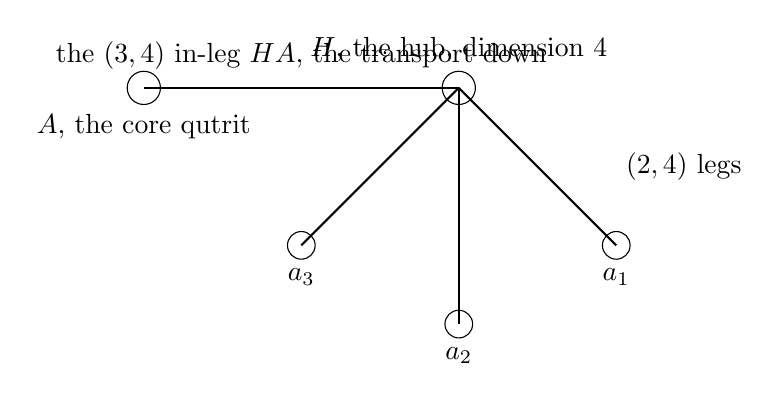
\begin{tikzpicture}[scale=1]
\filldraw[fill=white] (0,0) circle (6pt) node[above=6pt] {$H$, the hub, dimension 4};
\filldraw[fill=white] (-4,0) circle (6pt) node[below=6pt] {$A$, the core qutrit};
\filldraw[fill=white] (2,-2) circle (5pt) node[below=5pt] {$a_1$}; \filldraw[fill=white] (0,-3) circle (5pt) node[below=5pt] {$a_2$}; \filldraw[fill=white] (-2,-2) circle (5pt) node[below=5pt] {$a_3$};
\draw[thick] (-4,0) -- (0,0); \draw[thick] (0,0) -- (2,-2); \draw[thick] (0,0) -- (0,-3); \draw[thick] (0,0) -- (-2,-2);
\node at (-2,0) [above=3pt] {the $(3,4)$ in-leg $HA$, the transport down};
\node at (2,-1) [right] {$(2,4)$ legs};
\end{tikzpicture}\caption{The electron hub with its (3,4) in-leg to the core qutrit and its three (2,4) legs; the block is the hub read transported down the in-leg against the core read, and at the hub letters beyond Z it is cut at the leg $a_3$.}\end{figure}
\end{chproof}
\section{The mixing as the overlap Gram of the (3,4) pairings}\label{mod:VI-7-D543182-w-mxog}
\begin{chwall}[The mixing as the overlap Gram of the (3,4) pairings]\label{box:VI-7-D543182-w-mxog:1}
This result is conditional on the results it rests on, the open results among them consumed at their tables at their grades, the composition riding the lowest grade in its chain, and on the readings of its source disclosed at its register. The mixing as the overlap Gram of the (3,4) pairings across the bodies: at every one of the sixteen in-legs of the roster the pairing, the (3,4) pair ket read at the bases, carries the leg read into the hub frame, and the Gram of the pairings across the roster at one hub letter is the (3,3) overlap of the two core letters at every one of the eighty blocks, the hub frame dropping out at eighty of eighty; washed at the shared qutrit by the group it equals the quark-mixing-block entry cell for cell at seven of sixteen of the core-letter pairings at the plain reading, the pairing against the pairing, and at sixteen of sixteen at the conjugate reading, the first pairing read as the bra, the washed-overlap entry at sixteen of sixteen and the sink-basis entry at four of sixteen at the plain reading; the lepton-side open results re-met; the argument of every entry an exact twenty-fourth root at 600 of 720; so the face read is the second at the first parting, the Gram block of the pairing at the electron in-leg against the pairing at the muon in-leg at the core letters X against Z at every hub letter, washed at the shared qutrit: against the quark-mixing-block entry the Jarlskog element reads minus one ninth and one eighteenth at the Gram where the entry reads one ninth and minus one eighteenth, the block parting at the sign while the cells agree at 107 of 128; the second cell, the conjugate reading at the same block, reads the entry equal.
The first face, the mixing blocks the overlap Gram at every body with every block equal at every compared cell against the quark-mixing-block, washed-overlap and sink-basis entries and the lepton-side controls the same, reads no at the face cell, the blocks equal at seven of sixteen, sixteen of sixteen and four of sixteen; the second face, the first block parting named with both cells, reads yes at the Gram block of the electron pairing against the muon pairing at the core letters X against Z. Open is the sorting of the overlap: read as the bra against the ket, the conjugate reading of the conjugate-letter theorem, the Gram is the quark block cell for cell, and read as the ket against the ket it parts at the sign of the Jarlskog element at the first mixing pairing beyond the Z row.
\end{chwall}
\chstanding{an open result}
\chdeps{Definitions 1.1 to 1.6 and Theorem 166.1 and Open results 166.2 and 166.3}{no theorem beyond it at this release}
A (3,4) pairing at an in-leg carries the core read of the qutrit into the frame of the hub, and two pairings that meet at one hub frame, say the electron in-leg and the muon in-leg, overlap. Because the hub frame drops out, that overlap is the (3,3) overlap of the two core letters whatever the hub letter, and washed at the shared qutrit it is a three by three block whose entries are twenty-fourth roots of unity or zero. The question is whether this Gram across the bodies is the quark mixing block of the foregoing entry. It is, cell for cell at every core-letter pairing, when the first pairing is read as a bra, the sorting the conjugate-letter theorem prescribes, and it parts at the sign of the Jarlskog element when both pairings are read as kets; the open result names that first parting and lays neither reading.
\begin{chbridge}
The quark mixing matrix is the overlap of the bases that diagonalize the up-type and the down-type mass matrices, a unitary three by three matrix whose rephasing-invariant content is the Jarlskog invariant, and its complex conjugate describes the antiquarks \cite{Cabibbo1963,Jarlskog1985}. The correspondence is by name.
\end{chbridge}
\begin{chproof}[finite computation with its exact part]
The premises of this derivation are the axiom and the six definitions of chapter~\ref{mod:FRAMEWORK}, the mixing as the washed overlap and the CKM block of the present chapter, an open result, the mixing blocks at the (3,4) legs of the present chapter, an open result, the records, reads and the Born count of chapter~\ref{mod:I-3-records-reads-and-the-born-count-the-gain-lemma}, a theorem, and the hub step of chapter~\ref{mod:VI-1-hub-step-as-the-weak-interaction}, a theorem. The chain of premises runs back to the axiom through those chapters, and the longest such chain in this compendium is twelve chapters long.
\textit{The object.} The roster is the sixteen in-legs, thirteen at the five bodies with the tau sink as the tau and the tau web of the library beside, each a (3,4) link from a core qutrit to a hub ququart. The pairing at an in-leg and a letter pair, the core letter at the qutrit against the hub letter at the ququart, is the three by four matrix of overlaps of the leg rays with the four transported hub members, equal to the leg-register overlaps of the mixing-blocks entry at twenty of twenty pairs. The figure draws two in-legs meeting at one hub frame.
\textit{The procedure.} Read the rows of each pairing as unit rays through the hub frame. For each pair of in-legs and each pair of letter pairings at one hub letter, form the Gram of the rows of the first pairing against the rows of the second, 400 pairs of letter pairings and eighty designated blocks at one hub letter at both pairings. Wash each block at the shared qutrit by the group. Compare every block cell for cell, in the frozen cell order, against the quark-mixing-block entry, the washed-overlap entry and the sink-basis entry, at the plain reading, the pairing against the pairing, and at the conjugate reading, the first pairing as the bra.
\textit{The smallest instance.} Since the hub frame drops out, every one of the eighty blocks equals the (3,3) overlap of its two core letters, eighty of eighty. At the electron in-leg against the muon in-leg at the core letters X against Z the washed block carries the Jarlskog element
\begin{equation} J_{\mathrm{Gram}} = \big(0,\ 0,\ -\tfrac{1}{9},\ 0,\ 0,\ 0,\ \tfrac{1}{18},\ 0\big), \qquad J_{\mathrm{entry}} = \big(0,\ 0,\ \tfrac{1}{9},\ 0,\ 0,\ 0,\ -\tfrac{1}{18},\ 0\big), \end{equation}
in the eight coordinates of the ring, parting at the sign, the cells agreeing at 107 of 128 at this open result over the pairings; at the conjugate reading the same block reads $J = (0, 0, \tfrac{1}{9}, 0, 0, 0, -\tfrac{1}{18}, 0)$, equal to the entry. Over the sixteen core-letter pairings the plain reading equals the quark-mixing-block entry at seven of sixteen, the washed-overlap entry at sixteen of sixteen and the sink-basis entry at four of sixteen, and the conjugate reading equals the quark-mixing-block entry at sixteen of sixteen. Every entry of the eighty blocks is an exact twenty-fourth root or zero, 600 roots and 120 zeros of 720, and the phase group of the plain washed Z against X block has order three at the generator the eighth power of the twenty-fourth root; the mixing-phase open result is re-met at its composition cells.
\textit{The check.} The counter-tests alter the construction singly and read what moves. Striking a body moves the roster to fifteen in-legs and the first parting. Reading the (2,4) pairings in place of the (3,4) gives blocks of shape two by two and moves the first parting. Leaving the Gram unwashed moves the Born of the conjugate pairings off the flat value. Swapping the ends, the columns as the unit rays, gives blocks of shape four by four. Striking the text unmeets the gate. Each alteration moves the cells it names, five of five. The result was reproduced by an independent route, two engines built apart, equal at every cell, with the seventeen controls the same.
\chcert{80}
\begin{figure}[h]\centering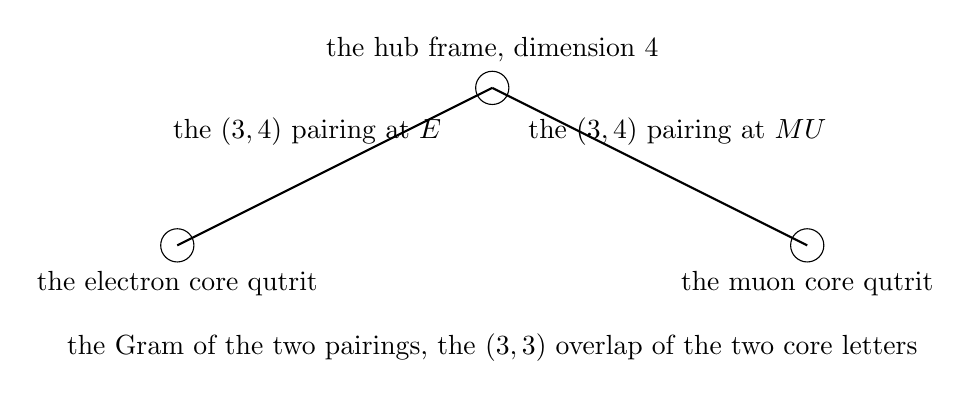
\begin{tikzpicture}[scale=1]
\filldraw[fill=white] (0,0) circle (6pt) node[above=6pt] {the hub frame, dimension 4};
\filldraw[fill=white] (-4,-2) circle (6pt) node[below=6pt] {the electron core qutrit};
\filldraw[fill=white] (4,-2) circle (6pt) node[below=6pt] {the muon core qutrit};
\draw[thick] (-4,-2) -- (0,0); \draw[thick] (4,-2) -- (0,0);
\node at (-2,-1) [above=4pt, xshift=-10pt] {the $(3,4)$ pairing at $E$};
\node at (2,-1) [above=4pt, xshift=10pt] {the $(3,4)$ pairing at $MU$};
\node at (0,-3) [below] {the Gram of the two pairings, the $(3,3)$ overlap of the two core letters};
\end{tikzpicture}\caption{Two (3,4) pairings meeting at one hub frame; their Gram is the (3,3) overlap of the two core letters whatever the hub letter, washed at the shared qutrit.}\end{figure}
\end{chproof}
\par\medskip\noindent{\itshape The mixing read, the next chapter turns to the process the weak sector is known for, beta decay.}\label{narr:close:6-7}\par
\section{Beta decay and the boson widths}\label{mod:VI-8-beta-decay-and-the-boson-widths}
\chdesig{8-8}{6-8}{VI-8-beta-decay-and-the-boson-widths}{VI-8-beta-decay-and-the-boson-widths}
\label{narr:open:6-8}Theorem~170.1 reads beta decay as the release at the plus-two arm and Open result~170.2 the boson widths as the hub-leg genre reads, both open results resting on the hub step and on the decay chapters of Part XII.
\begin{chtheorem}[Beta decay as the release at the plus-two arm]\label{box:VI-8-beta-decay-and-the-boson-widths:1}
Beta decay is read as the release at the plus-two arm at the literal closure reading of the decay graph: at that reading the catalogued neutron web is a non-sink carrying its dock edge at the plus-two arm, and the hub transfer at the dock of the arm, the hub unit of the released body attached at the dock by its in-leg together with the kept-leg hub at the same dock, adds with its end the cross-core object of the released body by an explicit isomorphism at dimensions and links, read through the hub at the order two of its (2,4) in-leg with the dressing of that link at both dressing readings, the readout 2916 at the hub spelling and the cell 1296 over 17689 at both spellings, so the beta rate cell is an output of the rate law at a non-sink. The two partings of the previous open result are closed at this reading: at the stop condition of the pairing move the neutron carried no forward edge, and the object the dock move added, a dock of one site at one link of measure 6, parted from the released body and from the cross-core object; at the literal closure reading the forward edge is present and the hub transfer adds the cross-core object, while the dock move of the previous reading remains the first admitted edge at the dock at which the release parts, its object a dock, printed beside; the deciding table is re-derived in Lean.
\end{chtheorem}
\chstanding{theorem, built at the literal closure reading}
\chdeps{Definitions 1.1 to 1.6, Theorem 158.1 and Open result 158.2, Theorem 203.1, Open result 203.2, Theorem 203.3, Open result 203.4, Theorem 203.5 and Open result 203.6 and Theorems 206.1 to 206.4}{no theorem beyond it at this release}
The box asks whether the rate law of this compendium, which assigns a rate to every unstable web, assigns one to the neutron. It does not, because the neutron is stable at the stop condition the decay graph uses, and the one move that acts at its plus-two arm adds a different object from the one a decay should release.
\begin{chwall}[The boson widths as the hub-leg genre reads]\label{box:VI-8-beta-decay-and-the-boson-widths:2}
The widths of the bosons are read as the hub-leg genre reads: the W and the Z bodies are sinks at the stop condition of the decay graph, so at the primary reading their widths are outputs of the rate law at neither, while at the two readings beside the carriers are non-sinks at all three with their widths defined at all three, the W and the Z at 270 over 49 each and the Higgs at 121 over 16.
\end{chwall}
\chstanding{open result, built and not closed}
\chdeps{Definitions 1.1 to 1.6, Theorem 158.1 and Open result 158.2, Theorem 203.1, Open result 203.2, Theorem 203.3, Open result 203.4, Theorem 203.5 and Open result 203.6 and Theorems 206.1 to 206.4}{no theorem beyond it at this release}
The second box does for the W, the Z and the Higgs what the first does for the neutron, at the stop condition the two carriers are stable and have no width, and only at the readings that admit every forward edge do all three decay, with exact widths and the W and Z widths equal.
\begin{chbridge}
What this chapter calls the release at the plus-two arm the literature calls the beta decay of the neutron and the dock edge its charged-current vertex. The correspondence is by name, and no width and no rate is displayed in this chapter.
\end{chbridge}
\begin{chproof}[finite computation]
The premises are the hub step as the weak interaction of chapter 6-1, an open result, the decay as the forward edge of a non-sink of chapter 9-1 and the rate as the washed square of the read of chapter 9-2, theorems. The chain from the axiom to this chapter is seven chapters long. The procedure of the first box, the input is the neutron web rebuilt from the seeds of the proton web with the arm turned down, 13 sites, 16 links, the measure 133, the hubs $H$ and $F$ at the hub rule, the dressing 81, the first power at the hub spelling and at the dock spelling
\begin{equation}
10773 = 133 \cdot 81, \qquad 133 ;
\end{equation}
the enumeration lists the forward edges of the neutron at the stop condition of the decay graph (none, the neutron a sink as the proton seed is) and the dock edges at the arm at the literal closure reading (two, the dock kind). The test is whether a forward edge of the construction leaves the neutron. The aggregation is the rate by the rate law, the readout of the dock move the measure it adds, 6, multiplied by the dressing. The smallest instance is the one dock edge at the arm, the readout 486 at the hub spelling and 6 at the dock spelling, the washed square 236196, and the rate cell in ticks
\begin{equation}
\Bigl(\frac{486}{10773}\Bigr)^{2} = \Bigl(\frac{6}{133}\Bigr)^{2} = \frac{36}{17689}
\end{equation}
at both spellings, the dressing canceling, and 72 over 17689 over the dock kind of two edges. The object the dock move adds is a dock of one site at one link, of measure 6, against the released object of the construction (four sites at the measure 28) and the cross-core object, parting at every reading. Of the four clauses of the first face, the forward edge of the construction reads no, the dock edge yes, the readout defined yes and the object the cross-core object no.

The procedure of the second box, the inputs are the three carriers, the W word, the Z word and the Higgs word, at their cataloged webs. The enumeration lists their forward edges at three readings, the stop condition of the decay graph, the literal closure and the forward-edge reading, every forward edge rebuilt from its token at the cataloged anatomy with the readout equal to the genre sum at 7 of 7 and at 39 of 39 over every carrier and the top. The test is whether the carrier is a non-sink. The aggregation is the width, the rate law summed over the forward edges. At the stop condition the carriers are non-sinks at 1 of 3 and the widths defined at 1 of 3, the first parting the W word. At the two readings beside the carriers are non-sinks at 3 of 3 with the widths
\begin{equation}
\frac{270}{49}, \qquad \frac{270}{49}, \qquad \frac{121}{16}, \qquad \frac{121/16}{270/49} = \frac{5929}{4320},
\end{equation}
the W over the Z one. The first powers re-met at 9 of 9 and the rate-row cells at 4 of 4.

\emph{Check.} At the neutron the muon cells of the rate law stand beside as the model of a rate at a non-sink, its first power 963 and its washed rate 34958 over 11449. At the carriers the counter-tests at their pinned letters 5 of 5 at the first and the controls the same at both routes but one at the first, a route writing a warning at every piece with every cell equal across the two. Each result was reproduced by an independent route, two engines at every capture byte for byte.
The beta rate as an output of the rate law is supplied by no cataloged non-sink at the stop condition, and the widths of the carriers stand at that reading undefined. Alpha decay is the matter of chapter 9-5.
\chcert{39}
\end{chproof}
\label{chend:VI-8-beta-decay-and-the-boson-widths}
\par\medskip\noindent{\itshape The results of the sector are gathered in the table of the next chapter.}\label{narr:close:6-8}\par

\clearpage
\part*{Part IX. The Junction\\[5pt]{\large The (3,3) cell}}
\label{atlaspart:09-cell-3-3-strong}
\addcontentsline{toc}{part}{Part IX. The Junction, The (3,3) cell}
\section*{Introduction to Part IX}\label{narr:part:VII}
\addcontentsline{toc}{section}{Introduction to Part IX}
The strong interaction sits at the cell (3,3) of the register matrix, the genre that pairs two qutrit ends and is the one genre at which no read survives at the first order. Part IX reads that fact as confinement, and then builds outward from it: the strong coupling as a closed read through the hadron body, the structure of the nucleon as a census of star records, the proton as a seeded sink, the ratio of the proton to the electron as a candidate read at second order, the hadron spectrum as a roster of saturated joined webs, the quark content and its flavors, and two chapters reserved for chiral breaking and the cap. The Part is the place where the saturation of chapter 1-5 does its heaviest work, because every hadron here is a sink of a seeded web.

The order of the nine chapters is dictated by one object, the star. A hadron in this construction is a star, a junction qutrit of degree three carrying the three quark bodies of the roster at its leaves, with the docks of the bodies its pendant pairs, and the quark is a body at the dark legs of that star. Confinement is read first because it is a statement about the legs of the star, the coupling second because it is a closed read through the star, the nucleon third because the star is counted record by record, the proton fourth because the star is seeded and saturated, and the mass ratio fifth because it is read at the second order at the same star. The spectrum and the quark content widen the view from one star to the joined webs of several stars and to the bodies at the leaves. The two chapters at the end are reserved, and the introduction names them as such. A reader who wants to see how far a finite construction can carry the strong interaction without a field should read chapters 7-1 and 7-4 together, the first for why no read survives at first order and the second for what the saturation does with that fact.

Chapter 7-1 reads confinement as the dark-genre readability in Theorem~171.1, resting on the link, the readability order and the probe, with the four readings beside, Open result~171.2, as an open result. The quark is a body at the dark legs of the star, the qutrit-qutrit links of the dark genre, and the readability of that genre is what confinement names, Theorem~171.1. The open result beside it types the dark-link cut by the read order of the cut link, first order at the qutrit-qubit genre at 162 of the 6296 cuts and second order at the dark genres at 6134, so that the construction admits a dark-link cut at the first order not, and at every dark cut the engine at order two reads the cut link with the twenty-eight records of the genre, Open result~171.2. Chapter 7-2 reads the strong coupling as the gluon closed read through the hadron body, Theorem~172.1, and states the running and the one genre per force, Open result~172.2, as an open result. The gluon closed qutrit-qutrit read at its pair is the closure sector twenty-eight at the gain three inside the chain sum, the coupling of the qutrit-qutrit genre an exact element of the field over the slot star with its order-two readout over the star, Theorem~172.1. The open result finds that the saturated proton carries no first-order colored readout at its three core legs, that the running reaches the Z body at no rung of the register tower, the Z body standing off the tower between the fourth and fifth rungs, and that one genre per force holds at the electromagnetic alone, Open result~172.2. These two chapters fix the (3,3) cell of the register matrix: the identification algebra su(3)+su(3)+u(1), the first non-vanishing read at order two, and the strong coupling as the office of the gluon pair ket, by name.

Chapters 7-3 to 7-5 read the nucleon. Theorem~174.1 reads nucleon structure as the star record census, Theorem~174.2 the junction sharing, the register, the form factor, the office and the pairable legs, with the five readings beside, Open result~174.3. The proton star, read link by link at the slot polarity, carries three thousand eight hundred fifty-seven records, each typed at an order, Theorem~174.1. At every one of the 250 junction sites of the roster the flat reduced diagonal of the pair ket at dimension three gives each leg one third of an end, the three thirds summing to one, and the register of the nucleon follows from the junction star at the share reading, the proton at 85 and the neutron at 125, Theorem~174.2. Open result~175.1 states the seeded saturation of the proton web as an open result, Theorem~175.2 the joined read at the roster stars, and Open result~175.4 the cap census at the proton sinks. The proton seed, the hub-attached three-quark web at the star core with the pair hub, ten sites and twelve links, is its own sink at wave zero at the stop condition of the pairing move, while under the twenty-eight catalogued moves the closure grows to twenty-five thousand five hundred fifty-eight webs, Open result~175.1. The roster stars of the proton and the neutron, each joined at the dock to the measurement web of its row, give the direct record sum to order three at the dock unit, every order exact and signed and the order-three term zero at every reading, Theorem~175.2. At every link of every proton sink of the roster census, seven webs at 80 links with 19 open docks, the record count at the primary map reading equals the cap of its genre at all 80 links, the colored links capped at all 22, Open result~175.4. Theorem~176.1 reads the mass ratio at the second-order read, a candidate and not a theorem, with its six readings beside in Open result~176.2. The lepton bodies are met again, the order of the read is exact and the ratio at the second-order read is exact, and the compendium displays the comparison nowhere, Theorem~176.1. Among the readings beside, the two ticks are exact and their squared ratio is two at the adopted unit, but the one unit tying the lattice step of the order register to the Killing norm of a direction step is fixed by no result of this work, the same missing unit the boost open result of Part IV names, Open result~176.2.

Chapters 7-6 and 7-7 widen the view to the spectrum and the quarks. Theorem~177.1 reads the hadron spectrum as the roster of saturated joined webs, Theorem~177.2 the mixed composition, the meson apparatus and the corollaries, and Open result~177.3 the direct sum at the deuteron as an open result. At the pairable set of the nucleon star, two docks at the proton star and one at the neutron star, the pairing move builds, up to four stars, exactly the joined webs admitted, and its sinks are exactly the saturated webs found, among them the chains of two neutron stars, of a proton between two neutrons and of two protons between two neutrons, Theorem~177.1. The register of the common support, sixteen at every qutrit-qubit dock and eighty-one at every qutrit-qutrit leg, is derived at the fourteen docks and the twelve legs of the six docked quark bodies and the two nucleon stars as one register at each reading, Theorem~177.2, while the direct two-exchange sum at the deuteron web meets the deuteron office of the earlier result at neither binding entry, the meson web direct sum being defined at every one of the twenty-one pairings of two qutrit cores admitted at the valence bound, Open result~177.3. Theorem~181.1 reads the quark register at the second-order junction read and Theorem~181.2 flavor as the rung name with the quark ladder, with the ladder at the saturated sinks in Theorem~181.4 and the quark offices as the star arm reads in Theorem~181.5, a theorem. The read engine run through every junction star at order two reads every leg with the entering link at the cut register, so the junction entry of a second read link is one exact object, eight at the cut reading, equal to the cut-reading bound at every one of the six quark bodies, with the share the color third, Theorem~181.1. Flavor is the rung name read at the corner, the three corner frames of the charged-lepton dark triangle at one, two and three hub legs equal to the three residues of the adopted naming at every corner, Theorem~181.2. The four heavy-flavor first powers, the strange, the charm, the bottom and the top, are outputs of the hub lowering at the saturated sinks, each a rank multiplied by a dressing, Theorem~181.4, and at the primary reading every arm of the two catalogued stars and every heavy sink is an office by the body-alone rule, the six arms at the first power 319 with the up and the down equal at the ratio one and every ratio among them an exact rational cell, Theorem~181.5. Chapters 7-8 and 7-9 are reserved, the table titled The chiral-breaking chapter (in chapter~\ref{mod:VII-8-chiral-breaking-and-the-theta-angle}, among the instruments) and the table titled The cap chapter (in chapter~\ref{mod:VII-9-mesons-and-the-nucleon-at-the-cap}, among the instruments): chiral breaking, the theta angle and the cap are named there, and the cap chapter carries six results at their own standing.

In the language of the literature, this Part names confinement, the strong coupling, the gluon, the nucleon form factor, the proton-to-electron mass ratio, the hadron spectrum, the mesons, the quarks, flavor, chiral breaking and the theta angle. The correspondence is by name at each. The boxes establish censuses of records at seeded sinks and reads at second order, and the candidate of chapter 7-5 is stated as a candidate.

The dependency lines of the Part point back to the link, the records, the probe and the saturation of Part I, and forward to the body-alone office rule of chapter 8-2, which the quark offices rest on. Confinement rests on the link, the readability order and the probe. The coupling rests on confinement, the quark register and the nucleon. The proton chapter rests on the saturation and the moves, and the spectrum on the proton and the pairing move. The reader who follows the derivation graph will find the proton of chapter 7-4 near the end of one of the longest chains in the compendium, and will find that the one number the Part is most often asked for, the mass ratio, is the one result the Part is most careful to call a candidate.
\section{Confinement as the dark-genre readability}\label{mod:VII-1-confinement-as-the-dark-genre-readability}
\chdesig{9-1}{7-1}{VII-1-confinement-as-the-dark-genre-readability}{VII-1-confinement-as-the-dark-genre-readability}
\label{narr:open:7-1}Confinement is read as a readability. Theorem~171.1 reads it as the dark-genre readability of the cell (3,3), the genre at which no read survives at the first order, and Open result~171.2 states the four readings beside as an open result.
\begin{chconditional}[Confinement as the dark-genre readability]\label{box:VII-1-confinement-as-the-dark-genre-readability:1}
Under the one-act clause and the open results it rests on, the hadron of the compendium is a star, a junction qutrit of degree three carrying the three quark bodies of the roster at its leaves, with the docks of the bodies its pendant pairs; the quark is a body at the dark legs of that star, the qutrit-qutrit links of the dark genre. At every one of the 494 qutrit-qutrit links of the roster the read engine carries no first-order readout and carries the second-order read, with the readout equal to the catalogued cells at every one of the 1368 dark cuts; at every one of the six quark bodies the open qutrit-qutrit end carries no first-order rest energy; and at every one of the eight stars a first-order Born reading passes through the qutrit-qubit docks alone. Confinement is therefore a corollary of the readability typing: the hadron masses are first-order objects, the proton register 85 and the neutron 125, and the quark offices are second-order objects, a quark appearing at the first order at no reading of the construction.
\end{chconditional}
\chstanding{conditional theorem}
\chdeps{Definitions 1.1 to 1.6, Theorems 9.1 to 9.7 and Open result 9.8 and Theorems 28.1 and 28.2, Open results 28.3 and 28.4 and Theorem 28.5}{Theorem 27.1, Theorem 172.1 and Open result 172.2, Theorems 174.1 and 174.2 and Open result 174.3, Open result 175.1, Theorem 175.2 and Open result 175.3, Theorems 181.1 and 181.2 and Open result 181.3 and Open result 257.1}
The box turns confinement into a statement about which links can be read at first order, the links of the genre a quark hangs from cannot, the links a hadron's docks are made of can, so a hadron shows up at first order and a quark never does.
\begin{chwall}[The four readings beside]\label{box:VII-1-confinement-as-the-dark-genre-readability:2}
The dark-link cut is typed by the read order of the cut link, first order at the qutrit-qubit genre at 162 of the 6296 cuts and second order at the dark genres at 6134, so the construction admits a dark-link cut at the first order not; at every dark cut the engine at order two reads the cut link with the twenty-eight records of the genre, and yet the change of the structure counts across a cut is not the change of the second-order reads at the deciding comparison; the star key at the dark cut is open at its deciding step; and the confined state with both ends open stands as an open result.
\end{chwall}
\chstanding{open results, four, built and not closed}
\chdeps{Definitions 1.1 to 1.6, Theorems 9.1 to 9.7 and Open result 9.8 and Theorems 28.1 and 28.2, Open results 28.3 and 28.4 and Theorem 28.5}{Theorem 27.1, Theorem 172.1 and Open result 172.2, Theorems 174.1 and 174.2 and Open result 174.3, Open result 175.1, Theorem 175.2 and Open result 175.3, Theorems 181.1 and 181.2 and Open result 181.3 and Open result 257.1}
The second box names the four readings beside the theorem that are tried and parted at their named steps.
\begin{chbridge}
What this chapter calls the readability typing of the dark genre the literature calls color confinement, the star a hadron, the body at a dark leg a quark and the qutrit-qubit docks the valence structure. The correspondence is by name.
\end{chbridge}
\begin{chproof}[census]
The premises are the link and its six genres of chapter 1-2 and the read at a register of chapter 1-6, definitions, the chain from the axiom five chapters long. The set counted is the set of links of the catalog, 1691 across the six genres,
\begin{equation}
1691 = 255 + 54 + 657 + 494 + 219 + 12
\end{equation}
at the genres (2,2), (2,3), (2,4), (3,3), (3,4) and (4,4), with the registers whole 16, 36, 64, 81, 144, 256 and cut 9, 24, 45, 64, 120, 225. The property tested is whether the read engine carries a first-order readout at the link, present if and only if the genre is in the readable set, the genres (2,2) and (2,3), and absent at the four dark genres. By kind. At the 494 links of the genre (3,3) the first-order readout is absent at 494 of 494 and the second-order read present at 494 of 494, the catalog of records at that genre 412 with the closed form of the count law
\begin{equation}
\frac{268 + 200\sqrt{3}}{419904}
\end{equation}
equal at 494 of 494. The reads of the construction at first order are 309, 255 at (2,2) and 54 at (2,3), at 0 links of the genre (3,3). At the six quark bodies, in the order up, charm, top, down, strange, bottom, the open (3,3) end stands at 6 of 6 with no first-order rest energy at 6 of 6, and at the eight stars a first-order Born face passes through the (2,3) docks at 8 of 8. The smallest cases are the proton and the neutron stars, the proton register 85 at the share face equal to the link sum, the neutron 125, the reduced factor and the Born factor
\begin{equation}
\frac{85}{85 + 67} = \frac{85}{152}, \qquad \frac{85^{2}}{85^{2} + 67^{2}} = \frac{7225}{11714},
\end{equation}
with 67 the electron unit, and the quark office a second-order object at the junction read, the read at the (3,3) end $67/82944 + 25\sqrt{3}/41472$ and its share over three legs $67/248832 + 25\sqrt{3}/124416$, equal to the recorded share at the nucleon legs at 6 of 6.

The four counts together, the first-order readout absent at every (3,3) link, the second-order read present at every one, no first-order rest energy at the open end of any quark body and a first-order Born face at every star, make confinement a corollary of the typing, the first link with a first-order readout, the first quark body with a first-order rest energy and the first body without an open (3,3) end all none.

\emph{Check.} The first cut of this entry stood beyond its own pin and was set aside, its content confirmed at a disjoint route at 0 differing cells over 2212, and the re-fire inside the pin reproduced every cell. The result was reproduced by an independent route, two engines at every capture byte for byte, its five counter-tests and twelve controls at their pinned letters.
\chcert{494}
\end{chproof}
\label{chend:VII-1-confinement-as-the-dark-genre-readability}
\par\medskip\noindent{\itshape Confinement read, the next chapter reads the coupling of the sector.}\label{narr:close:7-1}\par
\section{The strong coupling}\label{mod:VII-2-strong-coupling}
\chdesig{9-2}{7-2}{VII-2-strong-coupling}{VII-2-D543568-scds-t1}
\label{narr:open:7-2}Theorem~172.1 reads the strong coupling as the gluon closed read through the hadron body, and Open result~172.2 states the running and the one genre per force as an open result.
\begin{chconditional}[The strong coupling as the gluon closed read through the hadron body]\label{box:VII-2-strong-coupling:1}
Under the carrier as the closed-genre read, the coupling genre, confinement, the quark register and the nucleon mass, the gluon closed qutrit-qutrit read at its pair is the closure sector twenty-eight at the gain three inside the chain sum, the coupling of the qutrit-qutrit genre an exact element of the field over the slot star and its order-two readout over the star; the read rule of that genre follows from the readability typing, the legs of a qutrit-qutrit junction read at first order at none of three and at second order at three of three at both nucleon stars, and the strong coupling as the gluon closed read through the hadron body is defined at one reading of the derived read rule, with the register of the common support, sixteen at every qutrit-qubit dock and eighty-one at every qutrit-qutrit leg, derived from the link dimensions of the roster.
\end{chconditional}
\chstanding{conditional theorem}
\chdeps{Definitions 1.1 to 1.6, Theorems 9.1 to 9.7 and Open result 9.8 and Theorem 171.1 and Open result 171.2}{Theorem 173.1 and Theorems 177.1 and 177.2 and Open result 177.3}
The box defines the strong coupling of this compendium, the gluon is the closed read of the qutrit-qutrit genre, its closure sector is one exact number of the ring, and passing that read through the proton or the neutron at the register the common support fixes gives one exact element of the field at each face. The first reading of the same object at the first row of this entry is carried whole.
\begin{chwall}[The running and the one genre per force]\label{box:VII-2-strong-coupling:2}
The saturated proton carries no first-order coloured readout at its three core legs, and the running reaches the Z body at no rung of the register tower, the Z body standing off the tower between the fourth and fifth rungs; and one genre per force holds at the electromagnetic alone, the strong coupling being the root of no single genre at any register, its body factor passing five genres at the hadron body.
\end{chwall}
\chstanding{open results, two, built and not closed}
\chdeps{Definitions 1.1 to 1.6, Theorems 9.1 to 9.7 and Open result 9.8 and Theorem 171.1 and Open result 171.2}{Theorem 173.1 and Theorems 177.1 and 177.2 and Open result 177.3}
The second box names the two readings beside that part, the running of the coupling never lands on the Z body, and the strong force is not carried by one genre the way the electromagnetic one is.
\begin{chbridge}
What this chapter calls the gluon closed read the literature calls the strong coupling, the closure sector its value at the hadron scale and the register tower the renormalization scale, each the nearest object. The correspondence is by name, and the value of the coupling stands in the comparison table alone.
\end{chbridge}
\begin{chproof}[finite computation]
The premises are the link and its six genres of chapter 1-2, a definition, confinement of chapter 7-1, a theorem, and the framework. The chain from the axiom to this chapter is six chapters long. The procedure. The input is the count law of the (3,3) genre from its two end dimensions alone, the traceless slots 8 and 8, the roster 384 and the swap-fixed 16, the sectors odd 184, mixed-even 128, same-even 72 and closure 28 at the orders 0, 1, 1 and 2 and the gains 1, 3, 3 and 9,
\begin{equation}
412 = 184 + 200 + 28, \qquad 1036 = 184 \cdot 1 + 200 \cdot 3 + 28 \cdot 9 ,
\end{equation}
the records and the Born face, with the whole 81, the cut 64 and the star of order one $419904 = 81 \cdot 72^{2}$ and of order two $331776 = 576^{2}$. The enumeration takes the gluon word at its one qutrit-qutrit link, the carrier at the closed read with the closure sector 28 at the gain 9, and the two nucleon stars, the center at dimension 3 with three (3,3) legs at the register 9 each and the arms the cataloged quark bodies at their leaves, the proton at 11 sites, 11 links and the measure 85 with the arms up, up and down at the arm sum 150, the neutron at 15 sites, 16 links and the measure 125. The test reads the legs at both orders, the first-order leg count 0 of 3 and the second-order count 3 of 3 at both stars. The aggregation composes the closed read through the body at the register of the common support, the dock register 16 at the ratio one and the port register 81 at the ratio 81 over 16. The smallest instance is the share at one leg, one third of the junction read,
\begin{equation}
\frac{67}{248832} + \frac{25}{124416}\sqrt{3}, \qquad 3 \cdot \frac{67}{248832} = \frac{67}{82944}, \qquad 3 \cdot \frac{25}{124416} = \frac{25}{41472} ,
\end{equation}
and the deciding objects at the proton,
\begin{equation}
\frac{30885589}{4076863488} + \frac{5761675}{1019215872}\sqrt{3}
\end{equation}
at the dock face and the same over 81 over 16 at the port face, $30885589/20639121408 + (5761675/5159780352)\sqrt{3}$, exact at 4 of 4 objects over the two bodies and the two faces.

The one change from the first reading of the entry at its hadron body is the register of the common support in place of the product register, every other reading kept, and the two computations are equal at every cell. The readings of the September faces at both spellings stand printed beside, the visible face at the register 64 reading $67/16 + (25/8)\sqrt{3}$.

\emph{Check.} What would have broken the result, the typing of the 494 (3,3) links read at any first-order readout, found at none. The polarities and the spellings of the derived read rule coinciding at one reading, as they do. The result was reproduced by an independent route, two engines at every capture byte for byte, its five counter-tests at their pinned letters and its sixteen controls the same at both routes.
The first-order colored readout, which no roster link carries, the running at a rung that reaches the Z body and one genre per force beyond the electromagnetic stay open. The register growth of the saturated proton is the matter of chapter 7-4.
\chcert{494}
\end{chproof}
\label{chend:VII-2-strong-coupling}
\section{The strong coupling at the depth scale}\label{mod:VII-2-D543568-scds-t1}
\begin{chconditional}[The strong coupling at the depth scale]\label{box:VII-2-D543568-scds-t1:1}
This theorem is conditional on its parent results, the open results among them, the six-dressings open result, the depth-rule open result, the five running open results and the decoupling open result, read at their grades, the composition riding the lowest grade in its chain. The strong coupling at the depth scale is an element at every rung: at every rung of the established chains of the depth-metric open result the (3,3) dressing of the six-dressings entry, the register sum $268 + 200\sqrt{3}$ at the count-law spelling with $208 + 200\sqrt{3}$ at the package spelling beside, over the register at the rung, the origin 24 multiplied by the rung base 36 to the depth, 24, eight hundred sixty-four, 31104, 1119744 and 40310784 at the depths zero to four, is an exact element of the ring at 80 of 80 chain states and spellings; the running, the ratio of successive rungs, is one over thirty-six at 30 of 30 steps, equal to the per-rung factor of the running-per-rung open result at 21 of 21 steps of the chains; the scale at the rung is the count metric of the item, 96 multiplied by the depth, at 40 of 40; the cells touching the ququart fall off at the same ratio at 180 of 180 steps; the five running open results are instances of this ladder at five of five and the decoupling open result is re-named at its degree reading with its two readings beside met; both faces printed; the chains beside equal alike.
The first face, the dressing exact at every rung with the cells re-met, the ratio of successive rungs an exact element at every step with the scale the count metric, the heavy cells at the falloff with the running open results instances and the decoupling open result met or re-named, and the ratio equal to the per-rung factor at every step, reads yes; the second face, the first rung or open result parting named, reads no, the first parting none.
\end{chconditional}
\chstanding{a conditional theorem}
\chdeps{Definitions 1.1 to 1.6 and Theorem 172.1 and Open result 172.2}{no theorem beyond it at this release}
The coupling of the (3,3) genre at a scale is read as its dressing, the register sum of the records of two reads at that genre, over the register at a rung of the depth ladder. The register at a rung is the origin multiplied by the rung base to the depth, so the dressing at successive rungs falls by one factor, one over thirty-six, which is the per-rung factor the running open result already carries, and the scale at a rung is the count metric, ninety-six per rung. The dressings of the genres touching the ququart fall at the same rate over the same register, so nothing decouples faster than anything else at this ladder, and the five foregoing open results on the running of the coupling are each an instance of the one ladder at a rung. The coupling at a scale is one cell at every rung, and the theorem is conditional on the open results it instantiates.
\begin{chbridge}
The strong coupling of quantum chromodynamics runs with the scale, decreasing logarithmically at high momentum transfer by asymptotic freedom, and the heavy quarks decouple below their thresholds, each threshold matching the coupling across it \cite{Gross1973,Politzer1973}. The correspondence is by name.
\end{chbridge}
\begin{chproof}[finite computation with its exact part]
The premises of this derivation are the axiom and the six definitions of chapter~\ref{mod:FRAMEWORK}, the strong coupling of the present chapter, a theorem, the running of the coupling of chapter~\ref{mod:V-7-running-of-the-coupling}, a theorem, the six dressings at the six genres of chapter~\ref{mod:VIII-1-mass-unit-and-the-first-power}, an open result, and the depth, the growth order and the termination wave of chapter~\ref{mod:X-4-depth-the-growth-order-and-the-termination-wave}, a theorem. The chain of premises runs back to the axiom through those chapters, and the longest such chain in this compendium is twelve chapters long.
\textit{The object.} The depth ladder of the established chains, ten chains at the steps zero to three, the seven chains of the depth-metric open result and three beside, carries at each rung the register $R_{k} = 24\cdot 36^{k}$, the origin multiplied by the rung base to the depth, re-met at forty of forty against the register-tower entry. The figure draws the ladder with its registers.
\textit{The procedure.} At every rung of every chain read the (3,3) dressing of the six-dressings entry, the register sum $D_{33} = 268 + 200\sqrt{3}$ at the count-law spelling and $208 + 200\sqrt{3}$ at the package spelling, over the register at the rung. Take the ratio of successive rungs by the ring quotient. Read the scale at the rung as the count metric, 96 multiplied by the depth. Read the heavy cells, the (2,4) dressing $450 + 96\sqrt{2}$, the (3,4) dressing $685 + 296\sqrt{3}$ and the (4,4) dressing 2460, over the same register and their ratios. Re-read the five running open results and the decoupling open result at their partings as instances at a rung.
\textit{The smallest instance.} At the rungs zero to four of a chain,
\begin{equation} g_{k} = \frac{268 + 200\sqrt{3}}{24\cdot 36^{k}}, \qquad \frac{g_{k}}{g_{k-1}} = \frac{1}{36}, \qquad \mu_{k} = 96\,k , \end{equation}
so the dressing is an exact element at every rung, eighty of eighty over the chain states and the two spellings, the ratio is one over thirty-six at thirty of thirty steps and equals the per-rung factor of the running-per-rung open result at twenty-one of twenty-one steps of the chains, one over the rung base, and the scale is zero, 96, 192, 288 and 384 at the depths zero to four, equal to the count metric at forty of forty. The heavy cells over the same register fall off at the same ratio, $\tfrac{450 + 96\sqrt{2}}{24\cdot 36^{k}}$, $\tfrac{685 + 296\sqrt{3}}{24\cdot 36^{k}}$ and $\tfrac{2460}{24\cdot 36^{k}}$ at the ratio one over thirty-six, 180 of 180 steps, exact at 240 of 240 cells, so the decoupling at this ladder is the common register growth. The five running open results re-read at their partings are instances at a rung, five of five, and the decoupling open result is re-named at its degree reading. The readings beside, the ratio one over eighty-one at the own reading of the (3,3) genre and one at the fixed reading, are printed beside.
\textit{The check.} The counter-tests alter the construction singly and read what moves. Striking the electron at the rung two from the ladder reads the ratio at the rung three against the rung one as one over 1296 against the factor, the deciding cell moving with the first parting at the electron. Reading the (2,3) dressing in place of the (3,3) moves the dressing at every rung with the deciding cell standing. Reading the scale at the tower parts it from the count metric at the electron at the rung zero first. Striking the text unmeets the gate. Reading a chain with no (3,3) cell refuses the dressing at the photon word. Each alteration moves the cells it names, five of five. The result was reproduced by an independent route, two engines built apart, a map-and-fraction route against the second route, equal at every cell, with the sixteen controls the same.
\chcert{80}
\begin{figure}[h]\centering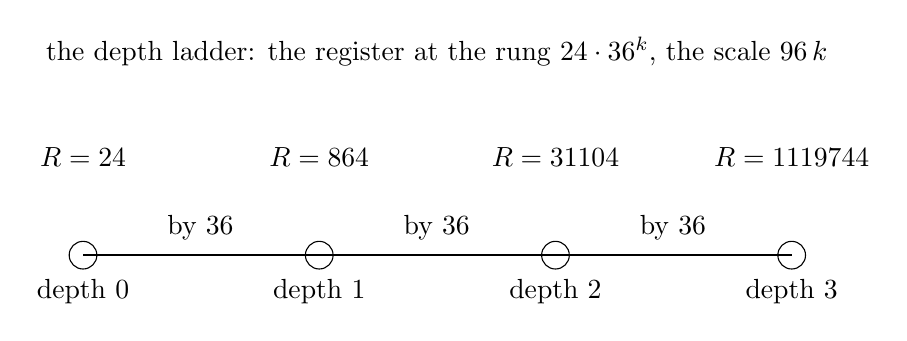
\begin{tikzpicture}[scale=1]
\foreach \x/\k/\r in {0/0/24, 3/1/864, 6/2/31104, 9/3/1119744} {\filldraw[fill=white] (\x,0) circle (5pt) node[below=5pt] {depth $\k$}; \node at (\x,1) [above] {$R = \r$};}
\draw[thick] (0,0) -- (9,0);
\node at (1,0) [above=2pt, xshift=14pt] {by 36}; \node at (4,0) [above=2pt, xshift=14pt] {by 36}; \node at (7,0) [above=2pt, xshift=14pt] {by 36};
\node at (4,2) [above=8pt, xshift=14pt] {the depth ladder: the register at the rung $24\cdot 36^{k}$, the scale $96\,k$};
\end{tikzpicture}\caption{The depth ladder of a chain with the register at each rung; the (3,3) dressing over that register falls by one over thirty-six per rung, the coupling at the depth scale.}\end{figure}
\end{chproof}
\par\medskip\noindent{\itshape The coupling in hand, the next three chapters read the nucleon.}\label{narr:close:7-2}\par
\section{Nucleon structure and the form factor}\label{mod:VII-3-nucleon-structure-and-the-form-factor}
\chdesig{9-3}{7-3}{VII-3-nucleon-structure-and-the-form-factor}{VII-3-nucleon-structure-and-the-form-factor}
\label{narr:open:7-3}Theorem~174.1 reads nucleon structure as the star record census, Theorem~174.2 the junction sharing, the register, the form factor, the office and the pairable legs, and Open result~174.3 the five readings beside.
\begin{chconditional}[Nucleon structure as the star record census]\label{box:VII-3-nucleon-structure-and-the-form-factor:1}
Under its parents, the nucleon of the compendium is a star, a junction qutrit of degree three carrying the three quark bodies of the roster at its leaves, with the docks of the bodies its pendant pairs and the hub of the down body its dressing. The proton star, read link by link at the slot polarity, carries three thousand eight hundred fifty-seven records, each typed at an order and censused at three sets, the docks, the legs and the hub, the fraction of the first-power sum at each set an exact rational, the three summing to one, so the parton structure of the nucleon is a census of the records of its star at their orders: the first-order qutrit-qubit docks read one set, the second-order qutrit-qutrit legs another and the hub a third.
\end{chconditional}
\chstanding{conditional theorem}
\chdeps{Definitions 1.1 to 1.6, Theorems 28.1 and 28.2, Open results 28.3 and 28.4 and Theorem 28.5 and Theorem 171.1 and Open result 171.2}{Open result 175.1, Theorem 175.2 and Open result 175.3, Theorem 176.1 and Open result 176.2, Theorems 177.1 and 177.2 and Open result 177.3, Theorems 181.1 and 181.2 and Open result 181.3 and Theorems 224.1 to 224.3 and Open result 224.4}
The box reads the proton as a small graph and counts, link by link, the records the read engine admits at each link and the order at which it admits them. The three kinds of link carry three disjoint sets of records, and the share of the star's first power that each set carries is an exact fraction.
\begin{chconditional}[The junction sharing, the register, the form factor, the office and the pairable legs]\label{box:VII-3-nucleon-structure-and-the-form-factor:2}
Under their parents, at every one of the 250 junction sites of the roster the flat reduced diagonal of the pair ket at dimension three gives each leg one third of an end, the three thirds summing to one; the register of the nucleon follows from the junction star at the share reading, the proton 85 and the neutron 125; the readout through the star at each of the seven admitted values of the transfer is exact at every one of the twenty-eight cells, so the form factor is an exact object of the star, its size the second transfer sum; the office of the star at the common support is an exact element of the field of root three at each nucleon; and the far set of every junction leg, transported, is a basis of the far support, so no junction leg pairs at a join.
\end{chconditional}
\chstanding{conditional theorems, five}
\chdeps{Definitions 1.1 to 1.6, Theorems 28.1 and 28.2, Open results 28.3 and 28.4 and Theorem 28.5 and Theorem 171.1 and Open result 171.2}{Open result 175.1, Theorem 175.2 and Open result 175.3, Theorem 176.1 and Open result 176.2, Theorems 177.1 and 177.2 and Open result 177.3, Theorems 181.1 and 181.2 and Open result 181.3 and Theorems 224.1 to 224.3 and Open result 224.4}
The second box gathers the five further theorems of the star, how a junction shares its ends among its legs, the register the star reaches, the readout at each admitted transfer, the office, and which legs can pair.
\begin{chwall}[The five readings beside]\label{box:VII-3-nucleon-structure-and-the-form-factor:3}
At every one of the nine lifts the definitions admit, the lifted norm carries the 172 records of the one link to their squared gains not; the local configuration of the electron web at its dock read is not the two-read one-pendant star of the fine-structure derivation; the site product of the located sites equals the first-order star read at the six quark stars but parts from it at both nucleon stars, 201 against 150 at the proton and 963 against 282 at the neutron; the junction star is not the root link opened at both ends; and the end-set selector at the junction face stands as an open result.
\end{chwall}
\chstanding{open results, five, built and not closed}
\chdeps{Definitions 1.1 to 1.6, Theorems 28.1 and 28.2, Open results 28.3 and 28.4 and Theorem 28.5 and Theorem 171.1 and Open result 171.2}{Open result 175.1, Theorem 175.2 and Open result 175.3, Theorem 176.1 and Open result 176.2, Theorems 177.1 and 177.2 and Open result 177.3, Theorems 181.1 and 181.2 and Open result 181.3 and Theorems 224.1 to 224.3 and Open result 224.4}
The third box names the five readings that were tried and parted. The joined Born square at both nucleons stands as a theorem at this chapter.
\begin{chbridge}
What this chapter calls the record census of the star the literature calls the parton structure of the nucleon, the dock set its valence quarks, the leg set its sea and glue, the readout at a transfer its form factor and the register its mass, each the nearest object. The correspondence is by name.
\end{chbridge}
\begin{chproof}[finite computation]
The premises are the read at a register of chapter 1-6, a definition, confinement of chapter 7-1, a theorem, and the framework. The chain from the axiom to this chapter is six chapters long. The procedure. The input is the proton star rebuilt from the cataloged bodies at its leaves, the center a site of dimension 3 with three (3,3) legs to the cores of the leaf bodies, eleven sites of dimensions 3, 3, 3, 3, 2, 2, 2, 4, 2, 2, 2 and eleven links, three legs of genre (3,3), three docks of genre (2,3), one hub leg of genre (3,4), three hub out-legs of genre (2,4) and one pair of genre (2,2), the measure
\begin{equation}
85 = 3 \cdot 9 + 3 \cdot 6 + 12 + 3 \cdot 8 + 4 ;
\end{equation}
the enumeration lists at every link the records of the count law of the read engine, for a passage of center dimension $c$ and far dimension $f$ at the traceless dimensions $A$ and $B$ the roster $4AB + A^{2} + B^{2}$, the swap-fixed $A + B$, the odd sector, the mixed-even sector $2AB$, the same-even sector and the closure, at the gains 1, $f$, $c$ and $cf$. The test types each record at its order. The aggregation censuses the records at the three sets and sums the first power over each. The smallest instance is the dock set, the three (2,3) docks at the first order,
\begin{equation}
516 = 237 + 144 + 126 + 9 ,
\end{equation}
the records by sector, odd, mixed-even, same-even and closure, at the orders 0, 1 and 2 as 237, 270 and 9 and the Born face 957. The three legs at the second order carry 1236 records and the hub a third set, the three together
\begin{equation}
3857
\end{equation}
records of the star.

From the first power at the link measure, the dressing a common factor, by the share of each set, we obtain the fractions at the reading of the first power, the docks 18 over 85, the legs 27 over 85 and the hub 40 over 85, summing to one,
\begin{equation}
\frac{18}{85} + \frac{27}{85} + \frac{40}{85} = 1 ,
\end{equation}
and at the dock-struck reading the docks 0, the legs 27 over 67 and the hub 40 over 67. For the second box the junction gives each leg one third of an end at 250 of 250 junction sites, the register of the proton 85 and the neutron 125 follow at the share reading, the readout at the seven admitted transfers is exact at 28 of 28 cells, the office at the common support is an element of the field of root three at each nucleon, and the far set of every junction leg transported is a basis of the far support.

\emph{Check.} One string of the catalog keying at thirteen of fifteen rows carried three trailing first-power cells inside the closed form at the pinned parse, a fault of the keying and of no cell, re-met at 15 of 15 by a second route and a third. The five counter-tests stand at their pinned letters and the controls the same at both routes with that one repaired. The result was reproduced by an independent route, two engines at every capture byte for byte.
The nuclear norm readout, the star as the electron dock read, the site product at the nucleon stars, the junction star as the root link opened and the end-set selector at the junction face stay open. The proton as a seeded sink is the matter of the next chapter.
\chcert{3857}
\end{chproof}
\begin{figure}[H]\centering
\begin{tikzpicture}[x=0.52pt,y=-0.52pt,baseline]
\clip (0,0) rectangle (900,540);
\fill[white] (0,0) rectangle (900,540);
\node[anchor=base west,inner sep=0pt,text=black,font=\fontsize{6.76}{8.112}\selectfont\ttfamily] at (12,22) {atlas U: U};
\node[anchor=base west,inner sep=0pt,text=black,font=\fontsize{6.24}{7.488}\selectfont\ttfamily] at (12,42) {membership 22:0;23:1;24:0;33:0;34:0;44:0; cells (2,3); links 1; sites 2; measure 6; census at the census};
\node[anchor=base west,inner sep=0pt,text=black,font=\fontsize{5.72}{6.864}\selectfont\ttfamily] at (12,62) {recorded office none; standing census:instrument;nucleon:theorem;roster:roster word; board quark};
\draw[draw=black,line width=1.04pt,dash pattern=on 1.04pt off 1.56pt] (100,250) -- (100,370);
\node[anchor=base,inner sep=0pt,text=black,font=\fontsize{5.72}{6.864}\selectfont\ttfamily] at (100,306) {(2,3)};
\filldraw[fill={rgb,255:red,208;green,208;blue,208},draw=black,line width=0.52pt] (100,250) circle (14);
\node[anchor=base,inner sep=0pt,text=black,font=\fontsize{6.24}{7.488}\selectfont\ttfamily] at (100,255) {3};
\node[anchor=base,inner sep=0pt,text=black,font=\fontsize{5.72}{6.864}\selectfont\ttfamily] at (100,280) {Q};
\filldraw[fill=white,draw=black,line width=0.52pt] (100,370) circle (14);
\node[anchor=base,inner sep=0pt,text=black,font=\fontsize{6.24}{7.488}\selectfont\ttfamily] at (100,375) {2};
\node[anchor=base,inner sep=0pt,text=black,font=\fontsize{5.72}{6.864}\selectfont\ttfamily] at (100,400) {n};
\node[anchor=base west,inner sep=0pt,text=black,font=\fontsize{5.72}{6.864}\selectfont\ttfamily] at (12,510) {the sites labelled by register (2 the qubit, white; 3 the qutrit, grey; 4 the ququart, dark); the links labelled by cell (p,q); a long dash an open dark link of the neutron row; a short dash a docked link at the rule R1};
\end{tikzpicture}
\caption{\texttt{U} (the quark), roster body: 2 sites, 1 links, the measure 6; the links at the cells (2,3); the membership 22:0; 23:1; 24:0; 33:0; 34:0; 44:0; 1 docked links at the rule R1 (Q-n); at the census of the six cells. Drawn at the anatomy atlas as its web, the sites labeled by register and the links by cell, from the nucleon register from the junction star.}\label{fig:VII-3-D520822-u-2e4e97}
\begin{center}\footnotesize\begin{adjustbox}{max width=\linewidth}\begin{tabular}{p{0.26\textwidth}p{0.68\textwidth}}\toprule
recorded office (the slot-count row) & no read of this body at the slot-count row \\
mass register (the mass-register row) & no read of this body at the mass-register row \\
\bottomrule\end{tabular}\end{adjustbox}\end{center}
\end{figure}
\begin{figure}[H]\centering
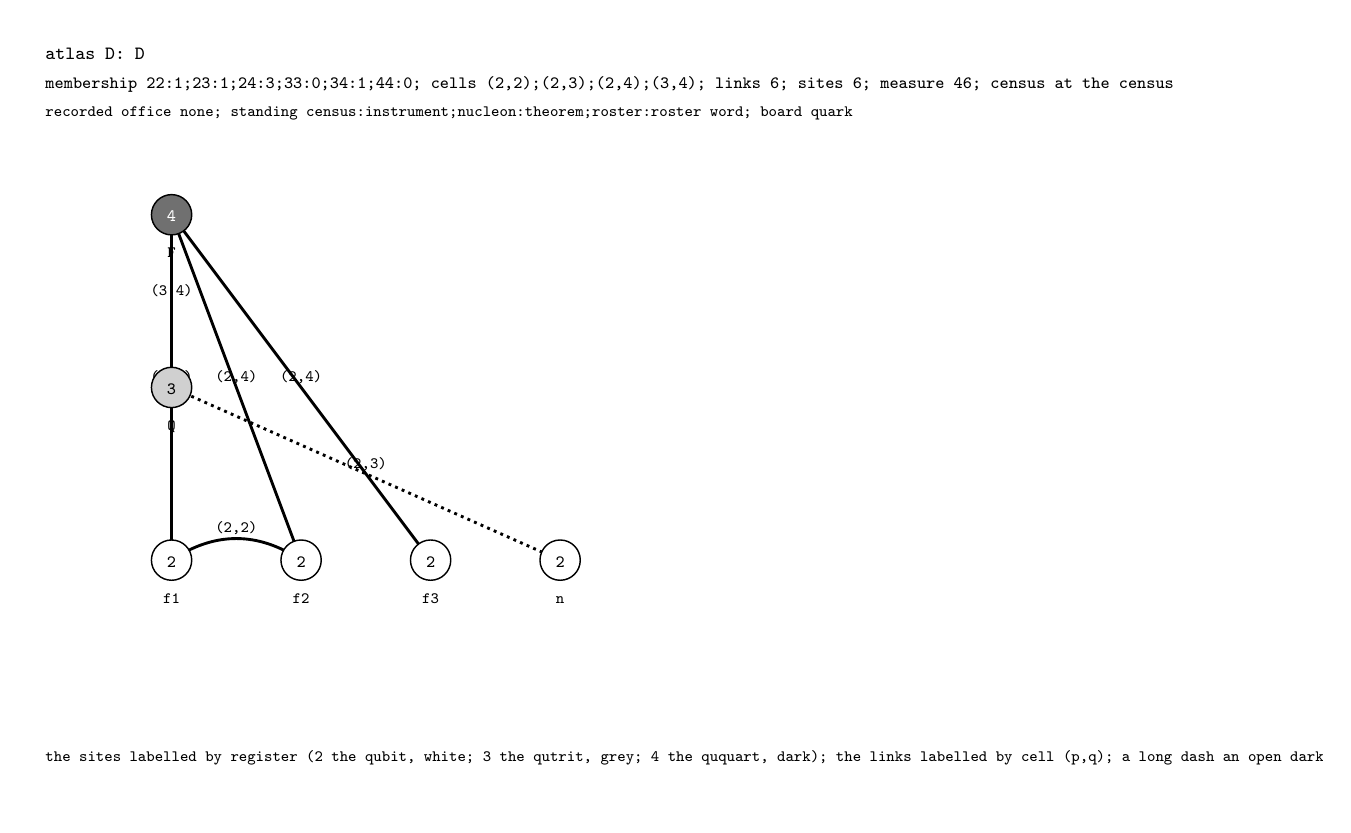
\begin{tikzpicture}[x=0.52pt,y=-0.52pt,baseline]
\clip (0,0) rectangle (900,540);
\fill[white] (0,0) rectangle (900,540);
\node[anchor=base west,inner sep=0pt,text=black,font=\fontsize{6.76}{8.112}\selectfont\ttfamily] at (12,22) {atlas D: D};
\node[anchor=base west,inner sep=0pt,text=black,font=\fontsize{6.24}{7.488}\selectfont\ttfamily] at (12,42) {membership 22:1;23:1;24:3;33:0;34:1;44:0; cells (2,2);(2,3);(2,4);(3,4); links 6; sites 6; measure 46; census at the census};
\node[anchor=base west,inner sep=0pt,text=black,font=\fontsize{5.72}{6.864}\selectfont\ttfamily] at (12,62) {recorded office none; standing census:instrument;nucleon:theorem;roster:roster word; board quark};
\draw[draw=black,line width=1.04pt] (100,130) -- (100,250);
\node[anchor=base,inner sep=0pt,text=black,font=\fontsize{5.72}{6.864}\selectfont\ttfamily] at (100,186) {(3,4)};
\draw[draw=black,line width=1.04pt] (100,130) -- (100,370);
\node[anchor=base,inner sep=0pt,text=black,font=\fontsize{5.72}{6.864}\selectfont\ttfamily] at (100,246) {(2,4)};
\draw[draw=black,line width=1.04pt] (100,130) -- (190,370);
\node[anchor=base,inner sep=0pt,text=black,font=\fontsize{5.72}{6.864}\selectfont\ttfamily] at (145,246) {(2,4)};
\draw[draw=black,line width=1.04pt] (100,130) -- (280,370);
\node[anchor=base,inner sep=0pt,text=black,font=\fontsize{5.72}{6.864}\selectfont\ttfamily] at (190,246) {(2,4)};
\draw[draw=black,line width=1.04pt,dash pattern=on 1.04pt off 1.56pt] (100,250) -- (370,370);
\node[anchor=base,inner sep=0pt,text=black,font=\fontsize{5.72}{6.864}\selectfont\ttfamily] at (235,306) {(2,3)};
\draw[draw=black,line width=1.04pt] (100,370) .. controls (130,350) and (160,350) .. (190,370);
\node[anchor=base,inner sep=0pt,text=black,font=\fontsize{5.72}{6.864}\selectfont\ttfamily] at (145,351) {(2,2)};
\filldraw[fill={rgb,255:red,112;green,112;blue,112},draw=black,line width=0.52pt] (100,130) circle (14);
\node[anchor=base,inner sep=0pt,text=white,font=\fontsize{6.24}{7.488}\selectfont\ttfamily] at (100,135) {4};
\node[anchor=base,inner sep=0pt,text=black,font=\fontsize{5.72}{6.864}\selectfont\ttfamily] at (100,160) {F};
\filldraw[fill={rgb,255:red,208;green,208;blue,208},draw=black,line width=0.52pt] (100,250) circle (14);
\node[anchor=base,inner sep=0pt,text=black,font=\fontsize{6.24}{7.488}\selectfont\ttfamily] at (100,255) {3};
\node[anchor=base,inner sep=0pt,text=black,font=\fontsize{5.72}{6.864}\selectfont\ttfamily] at (100,280) {Q};
\filldraw[fill=white,draw=black,line width=0.52pt] (100,370) circle (14);
\node[anchor=base,inner sep=0pt,text=black,font=\fontsize{6.24}{7.488}\selectfont\ttfamily] at (100,375) {2};
\node[anchor=base,inner sep=0pt,text=black,font=\fontsize{5.72}{6.864}\selectfont\ttfamily] at (100,400) {f1};
\filldraw[fill=white,draw=black,line width=0.52pt] (190,370) circle (14);
\node[anchor=base,inner sep=0pt,text=black,font=\fontsize{6.24}{7.488}\selectfont\ttfamily] at (190,375) {2};
\node[anchor=base,inner sep=0pt,text=black,font=\fontsize{5.72}{6.864}\selectfont\ttfamily] at (190,400) {f2};
\filldraw[fill=white,draw=black,line width=0.52pt] (280,370) circle (14);
\node[anchor=base,inner sep=0pt,text=black,font=\fontsize{6.24}{7.488}\selectfont\ttfamily] at (280,375) {2};
\node[anchor=base,inner sep=0pt,text=black,font=\fontsize{5.72}{6.864}\selectfont\ttfamily] at (280,400) {f3};
\filldraw[fill=white,draw=black,line width=0.52pt] (370,370) circle (14);
\node[anchor=base,inner sep=0pt,text=black,font=\fontsize{6.24}{7.488}\selectfont\ttfamily] at (370,375) {2};
\node[anchor=base,inner sep=0pt,text=black,font=\fontsize{5.72}{6.864}\selectfont\ttfamily] at (370,400) {n};
\node[anchor=base west,inner sep=0pt,text=black,font=\fontsize{5.72}{6.864}\selectfont\ttfamily] at (12,510) {the sites labelled by register (2 the qubit, white; 3 the qutrit, grey; 4 the ququart, dark); the links labelled by cell (p,q); a long dash an open dark link of the neutron row; a short dash a docked link at the rule R1};
\end{tikzpicture}
\caption{\texttt{D} (the quark), roster body: 6 sites, 6 links, the measure 46; the links at the cells (2,2), (2,3), (2,4), (3,4); the membership 22:1; 23:1; 24:3; 33:0; 34:1; 44:0; 1 docked links at the rule R1 (Q-n); at the census of the six cells. Drawn at the anatomy atlas as its web, the sites labeled by register and the links by cell, from the nucleon register from the junction star.}\label{fig:VII-3-D520822-d-8c290a}
\begin{center}\footnotesize\begin{adjustbox}{max width=\linewidth}\begin{tabular}{p{0.26\textwidth}p{0.68\textwidth}}\toprule
recorded office (the slot-count row) & no read of this body at the slot-count row \\
mass register (the mass-register row) & no read of this body at the mass-register row \\
\bottomrule\end{tabular}\end{adjustbox}\end{center}
\end{figure}
\label{chend:VII-3-nucleon-structure-and-the-form-factor}
\par\medskip\noindent{\itshape The structure read, the next chapter builds the proton as a sink.}\label{narr:close:7-3}\par
\section{The proton as a seeded sink}\label{mod:VII-4-proton-as-a-seeded-sink}
\chdesig{9-4}{7-4}{VII-4-proton-as-a-seeded-sink}{VII-4-proton-as-a-seeded-sink}
\label{narr:open:7-4}Open result~175.1 states the seeded saturation of the proton web, Theorem~175.2 the joined read at the roster stars, Open result~175.3 the six readings beside, and Open result~175.4 the cap census at the proton sinks.
\begin{chwall}[The seeded saturation of the proton web]\label{box:VII-4-proton-as-a-seeded-sink:1}
The proton seed, the hub-attached three-quark web at the star core with the pair hub, ten sites and twelve links, is its own sink at wave zero at the stop condition of the pairing move, so that the saturation of the proton seed under that move is the seed itself, while under the twenty-eight catalogued moves the closure grows to twenty-five thousand five hundred fifty-eight webs at wave four, unstopped at the candidate bound. On the one face the seed is a sink at wave zero with the first power 2727 at the hub spelling and 101 at the dock spelling; on the other face the saturation is unstopped at the bound and the candidate cell 8613 equals the first power at no sink of the bounded closure at any reading, the parting named with both objects, 2727 against 8613. Re-posed with the budget replaced by the site bound six of the closure without caps: the proton seed stands at ten sites beyond the bound, so the first chain reaching the bound is the seed itself at wave zero, a chain of length zero and its own sink, every one of its fifteen candidates under the twenty-eight moves refused at the bound at wave one, the closure the seed alone and exhausted at wave zero with no web within the bound and one beyond, the bound reached without a sink named within it; at the site bounds ten, eleven and twelve beside the closure stops at one, two and three webs with the seed its own sink at every reading, the first power 2727 at the hub spelling and 101 at the dock spelling re-met, and the sinks of this saturation at the site bands ten to twelve share no band with the forty-one forward sinks of the closure without caps at the bands three to six, so the two closures meet at no state by site count.
\end{chwall}
\chstanding{open result, built and not closed}
\chdeps{Definitions 1.1 to 1.6, Theorem 171.1 and Open result 171.2, Theorems 174.1 and 174.2 and Open result 174.3 and Open results 245.1 and 245.2, Theorem 245.3, Open results 245.4 to 245.8 and Theorem 245.9}{Open result 175.4 and Theorem 176.1 and Open result 176.2}
The box follows the proton as the thing the saturation of a seed reaches, which is not the roster star of the previous chapter but a web that grows from it. Under the one pairing move the seed is already stable, and under every move the growth does not stop inside the bound.
\begin{chconditional}[The joined read at the roster stars]\label{box:VII-4-proton-as-a-seeded-sink:2}
Under its parents, the roster stars of the proton and the neutron, each joined at the dock to the measurement web of its row, give the direct record sum to order three at the dock unit, every order exact and signed and the order-three term zero at every reading.
\end{chconditional}
\chstanding{conditional theorem}
\chdeps{Definitions 1.1 to 1.6, Theorem 171.1 and Open result 171.2, Theorems 174.1 and 174.2 and Open result 174.3 and Open results 245.1 and 245.2, Theorem 245.3, Open results 245.4 to 245.8 and Theorem 245.9}{Open result 175.4 and Theorem 176.1 and Open result 176.2}
The second box is the one theorem of the chapter, the roster star joined to its measuring web has an exact direct sum order by order.
\begin{chwall}[The six readings beside]\label{box:VII-4-proton-as-a-seeded-sink:3}
The one-link records weighted by the states they reach at the open ends of the star sum to 319, the both-ends Born count of the support-rank entry by construction, the identity of a count with itself and no reach; no sink of the site-bounded closure, 44341 sinks at wave four, and no sink of the clean twin reads the proton figure of the comparison table at any reading tried, so the candidate is refuted at the bounded closures; the first catalogued proton sink, eight sites and nine links at the unstruck measure 81, reads 2187 at the hub spelling of the measure law, equal at none of twelve readings to the figure of the proton row, the exact ratio 319 over 81; at the proton sink the three coloured junction legs are the open interior links of the confinement theorem, and the Born count over their open end sets is 3108, parting from the catalogued figure cell as an exact integer identity; the register grows from the seed to the saturated proton by the factor one, so the running at that growth is zero; and the proton sink record spectrum with no frame stands as an open result.
\end{chwall}
\chstanding{open results, six, built and not closed}
\chdeps{Definitions 1.1 to 1.6, Theorem 171.1 and Open result 171.2, Theorems 174.1 and 174.2 and Open result 174.3 and Open results 245.1 and 245.2, Theorem 245.3, Open results 245.4 to 245.8 and Theorem 245.9}{Open result 175.4 and Theorem 176.1 and Open result 176.2}
The third box names the readings of the proton as a sink that were tried and parted, every one leaving the proton row of the comparison table outside the comparison. The strong coupling at the junction of the saturated proton stands as a theorem at this chapter.
\begin{chbridge}
What this chapter calls the proton seed and its sink the literature calls the proton, the pairing move its binding and the first power at the sink its mass. The correspondence is by name, and the proton row of the comparison table stands outside the comparison at every reading produced.
\end{chbridge}
\begin{chproof}[finite computation]
The premises are the saturation with its seeds, waves and sinks of chapter 1-5, a theorem, confinement of chapter 7-1 and the nucleon star of chapter 7-3, theorems. The chain from the axiom to this chapter is seven chapters long. The procedure. The input is the proton seed, the hub-attached block of the star core and the pair hub, the center $J$ with a (3,3) leg to each quark, an up dock at each quark, the hub $H$ with a (3,4) leg from each quark and the pair, ten sites and twelve links, the measure
\begin{equation}
101 = 3 \cdot 9 + 3 \cdot 6 + 3 \cdot 12 + 2 \cdot 8 + 4 ,
\end{equation}
three in-legs at the hub rule and the hub beyond the valence bound at degree 5. The enumeration grows the closure from the seed wave by wave under the moves, every intermediate web printed at its measure, its unstruck measure, its in-leg count and its first powers. The test at every web is the stop condition, no closed-equal site with spare and the pairing move admitting no join. The aggregation counts the sinks by wave. The smallest instance is the seed itself, a sink at wave zero, with the first power at the hub spelling the unstruck measure multiplied by three to the in-legs and at the dock spelling the measure,
\begin{equation}
2727 = 101 \cdot 3^{3}, \qquad 101 ,
\end{equation}
and the display over the electron cell squared, $826281/4489$, compared with nothing here.

Under the pairing move alone the seed is the whole closure, stopped and exhausted at wave one. Under the twenty-eight moves the closure grows as
\begin{equation}
25558 = 1 + 12 + 252 + 7297 + 17996
\end{equation}
over the waves zero to four, unstopped at the candidate bound at the first slice of wave four, with 16946 sinks at the stop condition, by wave 1, 10, 170, 4249 and 12516. The neutron reading, the seed with one arm turned down, is its own sink alike with the first power 10773 at the hub spelling and 133 at the dock spelling, the additive difference from the proton 32 at the dock spelling and 8046 at the hub. The control, the cataloged electron as a seed, is its own sink at wave zero and re-meets its first power 201 and 67 at the readings striking the docks. The candidate cell 8613 equals the first power at no sink of the bounded closure at any reading, the parting of the box.

\emph{Check.} The self-loop count read zero at every wave of every closure. The electron control parts at the readings striking no dock, 237 and 79, and meets at the others. The result was reproduced by an independent route, two engines at every capture byte for byte, its four counter-tests at their pinned letters and its eleven controls the same at both routes.
The proton as a sink of the saturation stays open at every reading, the seeded saturation unstopped or parting, the first power at the sink no integer reading of the proton row, and the open count, the register growth and the record spectrum at their partings.
\chcert{25558}
\end{chproof}
\label{chend:VII-4-proton-as-a-seeded-sink}
\subsection{The cap census at the proton sinks}\label{mod:VII-4-D535254-w-prca}
\begin{chwall}[The cap census at the proton sinks]\label{box:VII-4-D535254-w-prca:1}
At every link of every proton sink of the roster census, seven webs at 80 links with 19 open docks, the record count at the primary map reading equals the cap of its genre at all 80 links, so every link is capped at the adopted typing, the coloured links capped at all 22 and the cap of every roster web met again at all seven, the 228 link-end caps at their genre cells. On the one face every link is capped; on the other face the readout of the first sink parts from the candidate and seed cells at both leg readings, 25839 at the counted reading and 8613 at the excluded reading against the cells 2871 and 2727, the parting named with both cells.
\end{chwall}
\chstanding{open result, built and not closed}
\chdeps{Definitions 1.1 to 1.6 and Open result 175.1, Theorem 175.2 and Open result 175.3}{no theorem beyond it at this release}
The box checks that every link of every proton-like stable web already carries as many records as its genre allows, and then asks whether the readout principle applied to such a capped web reproduces the two proton cells of the construction. It does not at either.
\begin{chbridge}
What this chapter calls the cap of a genre the literature calls the dimension of the record space of a link, the nearest object. The correspondence is by name, and the counts of this chapter are exact objects compared with nothing here.
\end{chbridge}
\begin{chproof}[finite computation]
The premises are the proton chapter above and the framework. The chain from the axiom to this result is eight chapters long. The procedure. The input is the roster of seven webs, the bound-respecting seed sink, the proton-web seed sink, the star-face sink and the cataloged star beside, the neutron twin and the two electron controls, at 80 links and 19 open docks. The enumeration lists every link with its genre and the record count at the map reading. The test compares the count with the cap of the genre, the Born count. The aggregation counts the capped and open links. The result is capped at 80 of 80 and open at 0 of 80, the first uncapped link none, the colored links capped at 22 of 22, the open-end links by the adopted definition of open 51 of 80 beside, and the caps of the seven webs and the 228 link-end caps re-met at their genre cells,
\begin{equation}
80 = 80 + 0, \qquad 22 = 22 + 0 .
\end{equation}
The smallest instance of the second face is the first sink, its readout at the principle, every open dock adding the Born count of the dock genre, reads 25839 at the counted reading and 8613 at the excluded reading at the dressings 27 and 9, against the candidate cell 2871 and the seed cell 2727,
\begin{equation}
25839 = 9 \cdot 2871, \qquad 8613 = 3 \cdot 2871, \qquad 8613 \neq 2727 ,
\end{equation}
parting at both leg readings, the one-dock reading beside equal at 2 of 2.

From the eleven comparisons against the dock numerators, by the same steps, the star-face sink equals the candidate at both readings and parts from the seed, and the two cataloged proton sinks equal at one leg reading at 0 of 2. The dressing equals the far-end cell of the parent at 4 of 4 webs carrying one.

\emph{Check.} The typed rows of every consumed table were counted at their records and apart. The comparisons stand at the exact integer differences and reduced ratios of the table. The result was reproduced by an independent route, two engines at every capture byte for byte, its counter-tests at their pinned letters and its controls the same at both routes.
The proton figure as the readout of a capped web stays equal at neither cataloged proton sink.
\chcert{80}
\end{chproof}
\label{chend:VII-4-D535254-w-prca}
\par\medskip\noindent{\itshape The proton built, the next chapter reads the ratio of its mass to the mass of the electron.}\label{narr:close:7-4}\par
\section{The proton-to-electron ratio: a candidate}\label{mod:VII-5-proton-to-electron-ratio-a-candidate}
\chdesig{9-5}{7-5}{VII-5-proton-to-electron-ratio-a-candidate}{VII-5-proton-to-electron-ratio-a-candidate}
\label{narr:open:7-5}Theorem~176.1 reads the mass ratio at the second-order read, a candidate stated as a candidate, with the six readings beside in Open result~176.2.
\begin{chconditional}[The mass ratio at the second-order read]\label{box:VII-5-proton-to-electron-ratio-a-candidate:1}
Under its parents, the lepton bodies are met again, the order of the read is exact, the ratio at the second-order read is exact and the Koide object is exact: the charged-lepton ratios at the second order of the read are exact objects compared at the direct reading of the comparison table, and this compendium displays them nowhere. The proton in the electron unit stands outside the comparison by orders at every reading the construction has produced, the object at those readings of another kind than the measured ratio as the comparison table types it.
\end{chconditional}
\chstanding{conditional theorem}
\chdeps{Definitions 1.1 to 1.6, Theorems 9.1 to 9.7 and Open result 9.8, Theorems 18.1 to 18.4 and Open results 18.5 and 18.6, Theorems 174.1 and 174.2 and Open result 174.3 and Open result 175.1, Theorem 175.2 and Open result 175.3}{no theorem beyond it at this release}
The box reads the three charged leptons at the second order of the read engine and forms their ratios and the Koide combination as exact numbers of the field. What it says about the proton is only that no reading yet produced lands the proton in the electron unit at the kind the comparison table asks.
\begin{chwall}[The six readings beside]\label{box:VII-5-proton-to-electron-ratio-a-candidate:2}
The two ticks are exact and their squared ratio is two at the adopted unit, but the one unit tying the lattice step of the order register to the Killing norm of a direction step is fixed by no result of this work; the support rank of the one qutrit-qubit link is the Born count over both ends, 319 as the sum over the 172 record letters, but the act readout sum of a roster web reading the link through its open qubit end is not that count at any catalogued web, the electron at its dock-struck rank 67 against 350; the 79 closed records of the one link fall into 48 mixed records, 28 at two qutrit slots and 3 at two qubit slots, and no union of these sets stands at 27, 40 or 12, the weights of the three sets of the roster electron, so the electron is forced at no partition of the closed records; the sinks of the bare link, the ladder at the hadron rows and the leg count from the end set each stand as an open result at their partings; the mass ratios at the one readout stand at this chapter.
\end{chwall}
\chstanding{open results, six, built and not closed}
\chdeps{Definitions 1.1 to 1.6, Theorems 9.1 to 9.7 and Open result 9.8, Theorems 18.1 to 18.4 and Open results 18.5 and 18.6, Theorems 174.1 and 174.2 and Open result 174.3 and Open result 175.1, Theorem 175.2 and Open result 175.3}{no theorem beyond it at this release}
The second box names the readings that would carry the candidate and part.
\begin{chbridge}
What this chapter calls the ratio at the second-order read the literature calls the ratio of two lepton masses and the Koide object the Koide combination, the nearest objects. The correspondence is by name, and this chapter displays no measured value.
\end{chbridge}
\begin{chproof}[exact]
The premises are the link and its six genres of chapter 1-2 and the reads and the Born count of chapter 1-3, definitions, the nucleon star of chapter 7-3 and the proton sink of chapter 7-4, the chain from the axiom eight chapters long. The set counted is the reads of the three charged-lepton bodies at the second order of the read engine, 1972 cells over the links at the three faces, the port of the construction, the struck links summed and the dark-port face, and the property tested is the exactness of the second-order term at each link, the first-order term multiplied by the square of the second-order readout. The exact part. From the first powers of the three bodies, the dock-struck rank multiplied by the hub dressing, we obtain at the first order the ratios
\begin{equation}
\frac{S_\mu}{S_e} = \frac{963}{201}, \qquad \Bigl(\frac{963}{201}\Bigr)^{2} = \frac{103041}{4489}, \qquad \Bigl(\frac{3969}{201}\Bigr)^{2} = \frac{1750329}{4489},
\end{equation}
the muon and the tau over the electron, equal to the earlier result at 2 of 2. From the electron at its port, the (2,3) link at the cut-register star 20736, by the second-order readout, we obtain
\begin{equation}
G_{2} = \frac{79}{20736} + \frac{1}{432}\sqrt{2} + \frac{7}{3456}\sqrt{3} + \frac{1}{6912}\sqrt{6} ,
\end{equation}
and the second-order term $T_{1} G_{2}^{2}$, nonzero, the mass at the first plus second order $T_{1}(1 + G_{2}^{2})$. At the port of the construction the muon-to-electron ratio keeps $103041/4489$ with the relative second-order part zero, the two bodies entering at a (2,3) port carrying one $G_{2}$ each. The Koide combination at the first order, the sum of the three masses over the square of the sum of their roots, the roots the first-power ratios with the sum $5133/67$ and the sum of squares $16720731/4489$, is
\begin{equation}
\frac{1857859}{2927521} = \frac{2}{3} - \frac{281465}{8782563} ,
\end{equation}
its departure from two thirds nonzero and exact.
\end{chproof}
\begin{chproof}[census]
The census part. By kind the second-order terms are nonzero at every link of the three bodies at the three faces, exact elements of the field at every cell, the three masses equal as rationals at 3 of 3 at the unit spelled as one, the smallest case the electron at its one port, the display above. The proton in the electron unit stands outside the comparison by orders at every reading produced.

\emph{Check.} Two keyings of the pinned engines, the unit mass spelled 1 against 1 over 1 and a histogram counted over the change table in place of the typing table, parted at one part of ten and one of eleven, every cell equal at a second route and a third with the keyings re-met. The Koide object at the first plus second order stands at the table of the entry as a rational of more than a hundred digits, and the result was reproduced by an independent route, two engines at every capture byte for byte, its counter-tests at their pinned letters.
\chcert{1972}
\end{chproof}
\label{chend:VII-5-proton-to-electron-ratio-a-candidate}
\par\medskip\noindent{\itshape From one hadron the thread widens to the whole spectrum.}\label{narr:close:7-5}\par
\section{The hadron spectrum and the mesons}\label{mod:VII-6-hadron-spectrum-and-the-mesons}
\chdesig{9-6}{7-6}{VII-6-hadron-spectrum-and-the-mesons}{VII-6-D543708-w-hdom}
\label{narr:open:7-6}Theorem~177.1 reads the hadron spectrum as the roster of saturated joined webs, Theorem~177.2 the mixed composition, the meson apparatus and the corollaries, and Open result~177.3 the direct sum at the deuteron as an open result.
\begin{chconditional}[The hadron spectrum as the roster of saturated joined webs]\label{box:VII-6-hadron-spectrum-and-the-mesons:1}
Under its parents, at the pairable set of the nucleon star, two docks at the proton star and one at the neutron star, the pairing move builds, up to four stars, exactly the joined webs admitted, and its sinks are exactly the saturated webs found: the chains of two neutron stars, of a proton between two neutrons and of two protons between two neutrons, the proton cycles of three and of four, the triton and the web of two neutrons and two protons, the deuteron never; beyond four stars the spectrum is the chain of proton stars capped by two neutron stars and the cycle of proton stars at every star count from five to the bound eight, two new sinks at every count, fourteen webs in all, each at the register 16 at the dock face and 81 at the port face.
\begin{figure}[H]\centering
\begin{adjustbox}{max width=\linewidth}\begin{tikzpicture}[x=0.52pt,y=-0.52pt,baseline]
\clip (0,0) rectangle (900,540);
\fill[white] (0,0) rectangle (900,540);
\node[anchor=base west,inner sep=0pt,text=black,font=\fontsize{6.76}{8.112}\selectfont\ttfamily] at (12,22) {atlas u\_docked: u\_docked};
\node[anchor=base west,inner sep=0pt,text=black,font=\fontsize{6.24}{7.488}\selectfont\ttfamily] at (12,42) {membership 22:0;23:2;24:0;33:0;34:0;44:0; cells (2,3); links 2; sites 3; measure 12; census at the census};
\node[anchor=base west,inner sep=0pt,text=black,font=\fontsize{5.72}{6.864}\selectfont\ttfamily] at (12,62) {recorded office none; standing census:instrument;hadron:open result;quark:open result;roster:roster word; board quark};
\draw[draw=black,line width=1.04pt,dash pattern=on 1.04pt off 1.56pt] (100,370) -- (100,250);
\node[anchor=base,inner sep=0pt,text=black,font=\fontsize{5.72}{6.864}\selectfont\ttfamily] at (100,306) {(2,3)};
\draw[draw=black,line width=1.04pt,dash pattern=on 1.04pt off 1.56pt] (100,250) -- (190,370);
\node[anchor=base,inner sep=0pt,text=black,font=\fontsize{5.72}{6.864}\selectfont\ttfamily] at (145,306) {(2,3)};
\filldraw[fill=white,draw=black,line width=0.52pt] (100,370) circle (14);
\node[anchor=base,inner sep=0pt,text=black,font=\fontsize{6.24}{7.488}\selectfont\ttfamily] at (100,375) {2};
\node[anchor=base,inner sep=0pt,text=black,font=\fontsize{5.72}{6.864}\selectfont\ttfamily] at (100,400) {Jd};
\filldraw[fill={rgb,255:red,208;green,208;blue,208},draw=black,line width=0.52pt] (100,250) circle (14);
\node[anchor=base,inner sep=0pt,text=black,font=\fontsize{6.24}{7.488}\selectfont\ttfamily] at (100,255) {3};
\node[anchor=base,inner sep=0pt,text=black,font=\fontsize{5.72}{6.864}\selectfont\ttfamily] at (100,280) {Q};
\filldraw[fill=white,draw=black,line width=0.52pt] (190,370) circle (14);
\node[anchor=base,inner sep=0pt,text=black,font=\fontsize{6.24}{7.488}\selectfont\ttfamily] at (190,375) {2};
\node[anchor=base,inner sep=0pt,text=black,font=\fontsize{5.72}{6.864}\selectfont\ttfamily] at (190,400) {n};
\node[anchor=base west,inner sep=0pt,text=black,font=\fontsize{5.72}{6.864}\selectfont\ttfamily] at (12,510) {the sites labelled by register (2 the qubit, white; 3 the qutrit, grey; 4 the ququart, dark); the links labelled by cell (p,q); a long dash an open dark link of the neutron row; a short dash a docked link at the rule R1};
\end{tikzpicture}\end{adjustbox}
\caption{\texttt{u\_docked} (the quark), hadron row body: 3 sites, 2 links, the measure 12; the links at the cells (2,3); the membership 22:0; 23:2; 24:0; 33:0; 34:0; 44:0; 2 docked links at the rule R1 (Q-n; Q-Jd); at the census of the six cells. Drawn at the anatomy atlas as its web, the sites labeled by register and the links by cell, from the hadron spectroscopy at the cap sinks.}\label{fig:VII-6-D540002-u-docked-e37fe0}
\begin{center}\footnotesize\begin{adjustbox}{max width=\linewidth}\begin{tabular}{p{0.26\textwidth}p{0.68\textwidth}}\toprule
recorded office (the slot-count row) & no read of this body at the slot-count row \\
mass register (the mass-register row) & the read KU: the class within the qubit and the qutrit; the first power 0; the office \texttt{0\textbar{}0\textbar{}0\textbar{}0}; zero; met yes; hubs none; in-legs none; dressing 1; ports Q-n; Q-Jd \\
\bottomrule\end{tabular}\end{adjustbox}\end{center}
\end{figure}
\begin{figure}[H]\centering
\begin{adjustbox}{max width=\linewidth}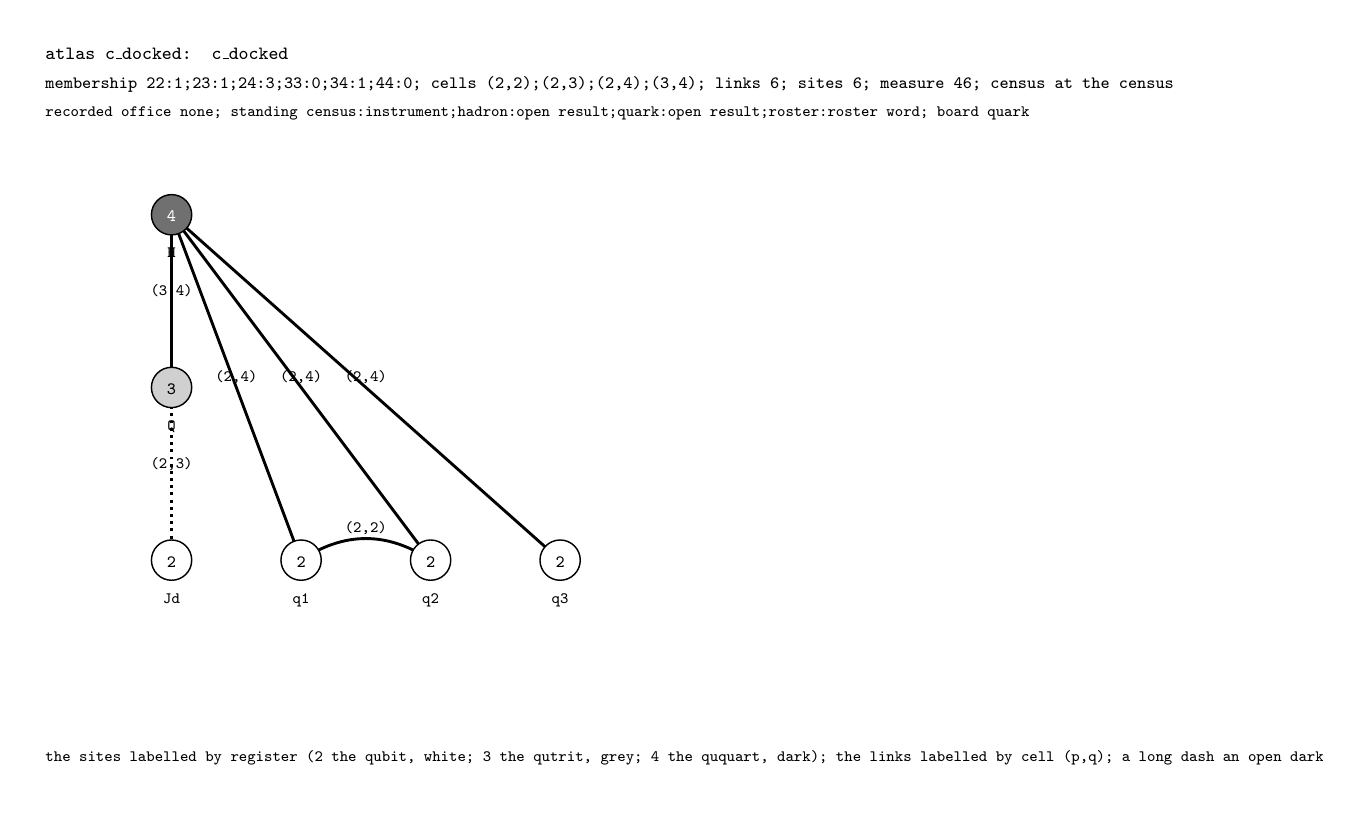
\begin{tikzpicture}[x=0.52pt,y=-0.52pt,baseline]
\clip (0,0) rectangle (900,540);
\fill[white] (0,0) rectangle (900,540);
\node[anchor=base west,inner sep=0pt,text=black,font=\fontsize{6.76}{8.112}\selectfont\ttfamily] at (12,22) {atlas c\_docked: c\_docked};
\node[anchor=base west,inner sep=0pt,text=black,font=\fontsize{6.24}{7.488}\selectfont\ttfamily] at (12,42) {membership 22:1;23:1;24:3;33:0;34:1;44:0; cells (2,2);(2,3);(2,4);(3,4); links 6; sites 6; measure 46; census at the census};
\node[anchor=base west,inner sep=0pt,text=black,font=\fontsize{5.72}{6.864}\selectfont\ttfamily] at (12,62) {recorded office none; standing census:instrument;hadron:open result;quark:open result;roster:roster word; board quark};
\draw[draw=black,line width=1.04pt] (100,130) -- (100,250);
\node[anchor=base,inner sep=0pt,text=black,font=\fontsize{5.72}{6.864}\selectfont\ttfamily] at (100,186) {(3,4)};
\draw[draw=black,line width=1.04pt] (100,130) -- (190,370);
\node[anchor=base,inner sep=0pt,text=black,font=\fontsize{5.72}{6.864}\selectfont\ttfamily] at (145,246) {(2,4)};
\draw[draw=black,line width=1.04pt] (100,130) -- (280,370);
\node[anchor=base,inner sep=0pt,text=black,font=\fontsize{5.72}{6.864}\selectfont\ttfamily] at (190,246) {(2,4)};
\draw[draw=black,line width=1.04pt] (100,130) -- (370,370);
\node[anchor=base,inner sep=0pt,text=black,font=\fontsize{5.72}{6.864}\selectfont\ttfamily] at (235,246) {(2,4)};
\draw[draw=black,line width=1.04pt,dash pattern=on 1.04pt off 1.56pt] (100,370) -- (100,250);
\node[anchor=base,inner sep=0pt,text=black,font=\fontsize{5.72}{6.864}\selectfont\ttfamily] at (100,306) {(2,3)};
\draw[draw=black,line width=1.04pt] (190,370) .. controls (220,350) and (250,350) .. (280,370);
\node[anchor=base,inner sep=0pt,text=black,font=\fontsize{5.72}{6.864}\selectfont\ttfamily] at (235,351) {(2,2)};
\filldraw[fill={rgb,255:red,112;green,112;blue,112},draw=black,line width=0.52pt] (100,130) circle (14);
\node[anchor=base,inner sep=0pt,text=white,font=\fontsize{6.24}{7.488}\selectfont\ttfamily] at (100,135) {4};
\node[anchor=base,inner sep=0pt,text=black,font=\fontsize{5.72}{6.864}\selectfont\ttfamily] at (100,160) {H};
\filldraw[fill=white,draw=black,line width=0.52pt] (100,370) circle (14);
\node[anchor=base,inner sep=0pt,text=black,font=\fontsize{6.24}{7.488}\selectfont\ttfamily] at (100,375) {2};
\node[anchor=base,inner sep=0pt,text=black,font=\fontsize{5.72}{6.864}\selectfont\ttfamily] at (100,400) {Jd};
\filldraw[fill={rgb,255:red,208;green,208;blue,208},draw=black,line width=0.52pt] (100,250) circle (14);
\node[anchor=base,inner sep=0pt,text=black,font=\fontsize{6.24}{7.488}\selectfont\ttfamily] at (100,255) {3};
\node[anchor=base,inner sep=0pt,text=black,font=\fontsize{5.72}{6.864}\selectfont\ttfamily] at (100,280) {Q};
\filldraw[fill=white,draw=black,line width=0.52pt] (190,370) circle (14);
\node[anchor=base,inner sep=0pt,text=black,font=\fontsize{6.24}{7.488}\selectfont\ttfamily] at (190,375) {2};
\node[anchor=base,inner sep=0pt,text=black,font=\fontsize{5.72}{6.864}\selectfont\ttfamily] at (190,400) {q1};
\filldraw[fill=white,draw=black,line width=0.52pt] (280,370) circle (14);
\node[anchor=base,inner sep=0pt,text=black,font=\fontsize{6.24}{7.488}\selectfont\ttfamily] at (280,375) {2};
\node[anchor=base,inner sep=0pt,text=black,font=\fontsize{5.72}{6.864}\selectfont\ttfamily] at (280,400) {q2};
\filldraw[fill=white,draw=black,line width=0.52pt] (370,370) circle (14);
\node[anchor=base,inner sep=0pt,text=black,font=\fontsize{6.24}{7.488}\selectfont\ttfamily] at (370,375) {2};
\node[anchor=base,inner sep=0pt,text=black,font=\fontsize{5.72}{6.864}\selectfont\ttfamily] at (370,400) {q3};
\node[anchor=base west,inner sep=0pt,text=black,font=\fontsize{5.72}{6.864}\selectfont\ttfamily] at (12,510) {the sites labelled by register (2 the qubit, white; 3 the qutrit, grey; 4 the ququart, dark); the links labelled by cell (p,q); a long dash an open dark link of the neutron row; a short dash a docked link at the rule R1};
\end{tikzpicture}\end{adjustbox}
\caption{\texttt{c\_docked} (the quark), hadron row body: 6 sites, 6 links, the measure 46; the links at the cells (2,2), (2,3), (2,4), (3,4); the membership 22:1; 23:1; 24:3; 33:0; 34:1; 44:0; 1 docked links at the rule R1 (Q-Jd); at the census of the six cells. Drawn at the anatomy atlas as its web, the sites labeled by register and the links by cell, from the hadron spectroscopy at the cap sinks.}\label{fig:VII-6-D540002-c-docked-e456cf}
\begin{center}\footnotesize\begin{adjustbox}{max width=\linewidth}\begin{tabular}{p{0.26\textwidth}p{0.68\textwidth}}\toprule
recorded office (the slot-count row) & no read of this body at the slot-count row \\
mass register (the mass-register row) & the read KC: the class touching the ququart; the first power 120; the office \texttt{47776588143529/3317760000\textbar{}661/4050\textbar{}5069/41472000\textbar{}0}; nonzero; met yes; hubs H; in-legs q-h; dressing 3; ports H-q3; Q-Jd \\
\bottomrule\end{tabular}\end{adjustbox}\end{center}
\end{figure}
\begin{figure}[H]\centering
\begin{adjustbox}{max width=\linewidth}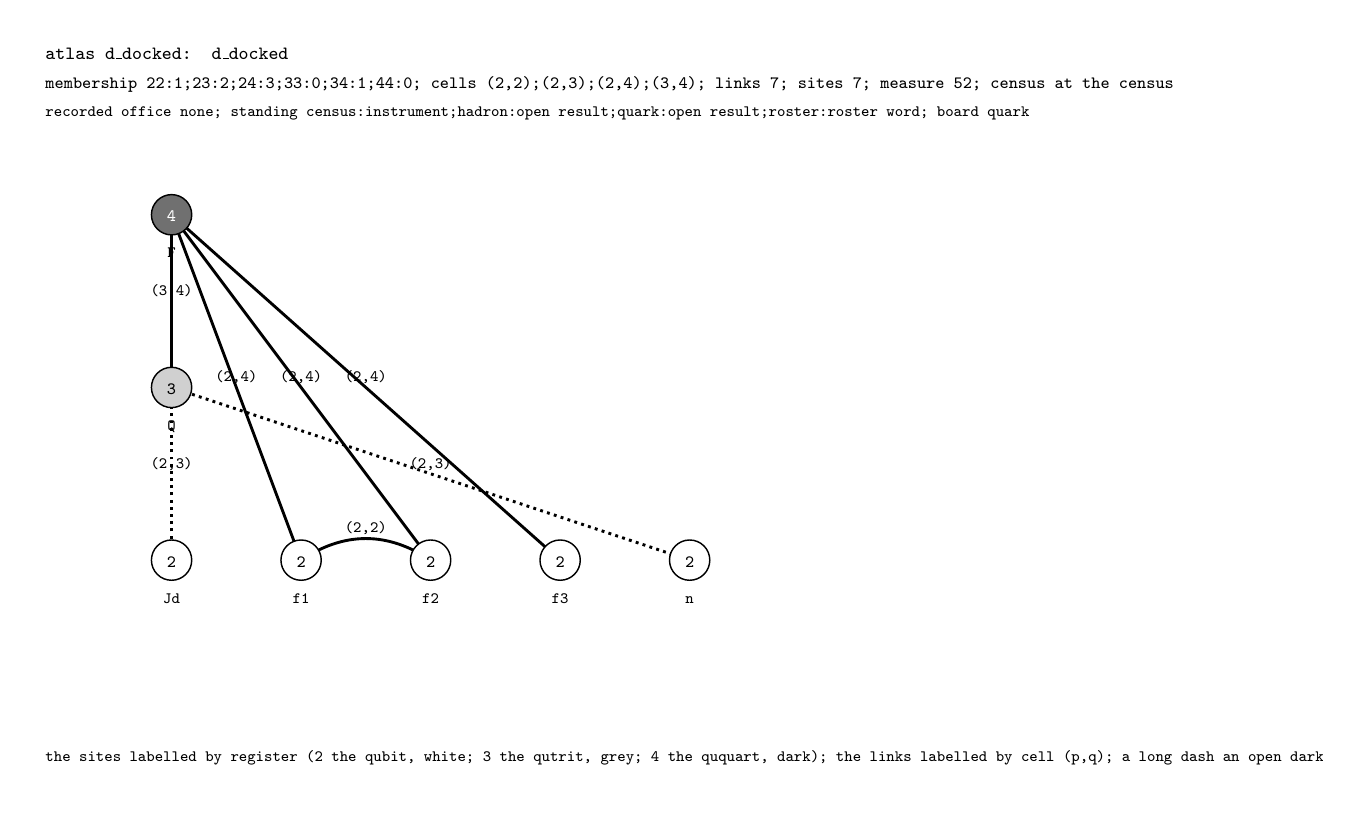
\begin{tikzpicture}[x=0.52pt,y=-0.52pt,baseline]
\clip (0,0) rectangle (900,540);
\fill[white] (0,0) rectangle (900,540);
\node[anchor=base west,inner sep=0pt,text=black,font=\fontsize{6.76}{8.112}\selectfont\ttfamily] at (12,22) {atlas d\_docked: d\_docked};
\node[anchor=base west,inner sep=0pt,text=black,font=\fontsize{6.24}{7.488}\selectfont\ttfamily] at (12,42) {membership 22:1;23:2;24:3;33:0;34:1;44:0; cells (2,2);(2,3);(2,4);(3,4); links 7; sites 7; measure 52; census at the census};
\node[anchor=base west,inner sep=0pt,text=black,font=\fontsize{5.72}{6.864}\selectfont\ttfamily] at (12,62) {recorded office none; standing census:instrument;hadron:open result;quark:open result;roster:roster word; board quark};
\draw[draw=black,line width=1.04pt] (100,130) -- (100,250);
\node[anchor=base,inner sep=0pt,text=black,font=\fontsize{5.72}{6.864}\selectfont\ttfamily] at (100,186) {(3,4)};
\draw[draw=black,line width=1.04pt] (100,130) -- (190,370);
\node[anchor=base,inner sep=0pt,text=black,font=\fontsize{5.72}{6.864}\selectfont\ttfamily] at (145,246) {(2,4)};
\draw[draw=black,line width=1.04pt] (100,130) -- (280,370);
\node[anchor=base,inner sep=0pt,text=black,font=\fontsize{5.72}{6.864}\selectfont\ttfamily] at (190,246) {(2,4)};
\draw[draw=black,line width=1.04pt] (100,130) -- (370,370);
\node[anchor=base,inner sep=0pt,text=black,font=\fontsize{5.72}{6.864}\selectfont\ttfamily] at (235,246) {(2,4)};
\draw[draw=black,line width=1.04pt,dash pattern=on 1.04pt off 1.56pt] (100,370) -- (100,250);
\node[anchor=base,inner sep=0pt,text=black,font=\fontsize{5.72}{6.864}\selectfont\ttfamily] at (100,306) {(2,3)};
\draw[draw=black,line width=1.04pt,dash pattern=on 1.04pt off 1.56pt] (100,250) -- (460,370);
\node[anchor=base,inner sep=0pt,text=black,font=\fontsize{5.72}{6.864}\selectfont\ttfamily] at (280,306) {(2,3)};
\draw[draw=black,line width=1.04pt] (190,370) .. controls (220,350) and (250,350) .. (280,370);
\node[anchor=base,inner sep=0pt,text=black,font=\fontsize{5.72}{6.864}\selectfont\ttfamily] at (235,351) {(2,2)};
\filldraw[fill={rgb,255:red,112;green,112;blue,112},draw=black,line width=0.52pt] (100,130) circle (14);
\node[anchor=base,inner sep=0pt,text=white,font=\fontsize{6.24}{7.488}\selectfont\ttfamily] at (100,135) {4};
\node[anchor=base,inner sep=0pt,text=black,font=\fontsize{5.72}{6.864}\selectfont\ttfamily] at (100,160) {F};
\filldraw[fill=white,draw=black,line width=0.52pt] (100,370) circle (14);
\node[anchor=base,inner sep=0pt,text=black,font=\fontsize{6.24}{7.488}\selectfont\ttfamily] at (100,375) {2};
\node[anchor=base,inner sep=0pt,text=black,font=\fontsize{5.72}{6.864}\selectfont\ttfamily] at (100,400) {Jd};
\filldraw[fill={rgb,255:red,208;green,208;blue,208},draw=black,line width=0.52pt] (100,250) circle (14);
\node[anchor=base,inner sep=0pt,text=black,font=\fontsize{6.24}{7.488}\selectfont\ttfamily] at (100,255) {3};
\node[anchor=base,inner sep=0pt,text=black,font=\fontsize{5.72}{6.864}\selectfont\ttfamily] at (100,280) {Q};
\filldraw[fill=white,draw=black,line width=0.52pt] (190,370) circle (14);
\node[anchor=base,inner sep=0pt,text=black,font=\fontsize{6.24}{7.488}\selectfont\ttfamily] at (190,375) {2};
\node[anchor=base,inner sep=0pt,text=black,font=\fontsize{5.72}{6.864}\selectfont\ttfamily] at (190,400) {f1};
\filldraw[fill=white,draw=black,line width=0.52pt] (280,370) circle (14);
\node[anchor=base,inner sep=0pt,text=black,font=\fontsize{6.24}{7.488}\selectfont\ttfamily] at (280,375) {2};
\node[anchor=base,inner sep=0pt,text=black,font=\fontsize{5.72}{6.864}\selectfont\ttfamily] at (280,400) {f2};
\filldraw[fill=white,draw=black,line width=0.52pt] (370,370) circle (14);
\node[anchor=base,inner sep=0pt,text=black,font=\fontsize{6.24}{7.488}\selectfont\ttfamily] at (370,375) {2};
\node[anchor=base,inner sep=0pt,text=black,font=\fontsize{5.72}{6.864}\selectfont\ttfamily] at (370,400) {f3};
\filldraw[fill=white,draw=black,line width=0.52pt] (460,370) circle (14);
\node[anchor=base,inner sep=0pt,text=black,font=\fontsize{6.24}{7.488}\selectfont\ttfamily] at (460,375) {2};
\node[anchor=base,inner sep=0pt,text=black,font=\fontsize{5.72}{6.864}\selectfont\ttfamily] at (460,400) {n};
\node[anchor=base west,inner sep=0pt,text=black,font=\fontsize{5.72}{6.864}\selectfont\ttfamily] at (12,510) {the sites labelled by register (2 the qubit, white; 3 the qutrit, grey; 4 the ququart, dark); the links labelled by cell (p,q); a long dash an open dark link of the neutron row; a short dash a docked link at the rule R1};
\end{tikzpicture}\end{adjustbox}
\caption{\texttt{d\_docked} (the quark), hadron row body: 7 sites, 7 links, the measure 52; the links at the cells (2,2), (2,3), (2,4), (3,4); the membership 22:1; 23:2; 24:3; 33:0; 34:1; 44:0; 2 docked links at the rule R1 (Q-n; Q-Jd); at the census of the six cells. Drawn at the anatomy atlas as its web, the sites labeled by register and the links by cell, from the hadron spectroscopy at the cap sinks.}\label{fig:VII-6-D540002-d-docked-984193}
\begin{center}\footnotesize\begin{adjustbox}{max width=\linewidth}\begin{tabular}{p{0.26\textwidth}p{0.68\textwidth}}\toprule
recorded office (the slot-count row) & no read of this body at the slot-count row \\
mass register (the mass-register row) & the read KD: the class touching the ququart; the first power 120; the office \texttt{47776588143529/3317760000\textbar{}661/4050\textbar{}5069/41472000\textbar{}0}; nonzero; met yes; hubs F; in-legs q-f; dressing 3; ports Q-n; F-f3; Q-Jd \\
\bottomrule\end{tabular}\end{adjustbox}\end{center}
\end{figure}
\begin{figure}[H]\centering
\begin{adjustbox}{max width=\linewidth}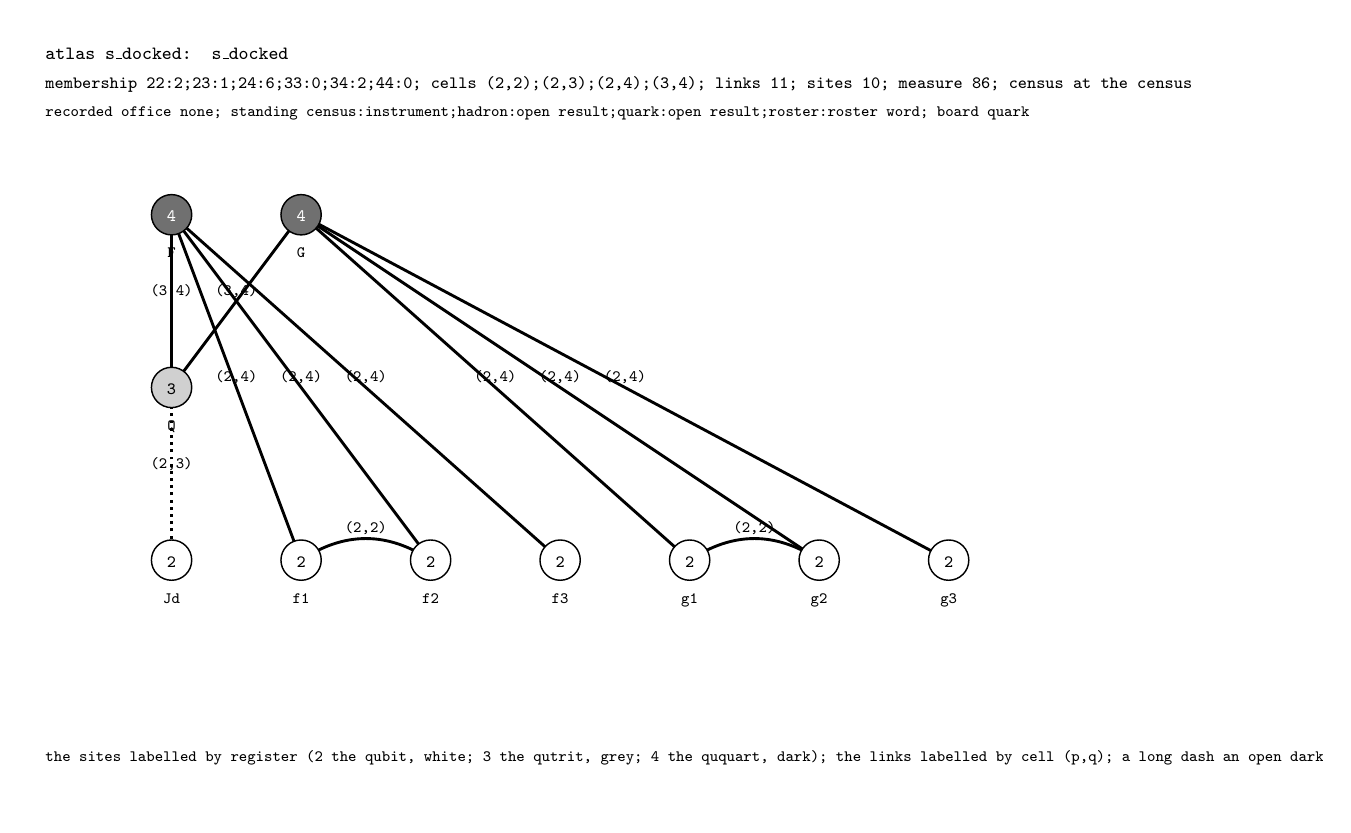
\begin{tikzpicture}[x=0.52pt,y=-0.52pt,baseline]
\clip (0,0) rectangle (900,540);
\fill[white] (0,0) rectangle (900,540);
\node[anchor=base west,inner sep=0pt,text=black,font=\fontsize{6.76}{8.112}\selectfont\ttfamily] at (12,22) {atlas s\_docked: s\_docked};
\node[anchor=base west,inner sep=0pt,text=black,font=\fontsize{6.24}{7.488}\selectfont\ttfamily] at (12,42) {membership 22:2;23:1;24:6;33:0;34:2;44:0; cells (2,2);(2,3);(2,4);(3,4); links 11; sites 10; measure 86; census at the census};
\node[anchor=base west,inner sep=0pt,text=black,font=\fontsize{5.72}{6.864}\selectfont\ttfamily] at (12,62) {recorded office none; standing census:instrument;hadron:open result;quark:open result;roster:roster word; board quark};
\draw[draw=black,line width=1.04pt] (100,130) -- (100,250);
\node[anchor=base,inner sep=0pt,text=black,font=\fontsize{5.72}{6.864}\selectfont\ttfamily] at (100,186) {(3,4)};
\draw[draw=black,line width=1.04pt] (100,130) -- (190,370);
\node[anchor=base,inner sep=0pt,text=black,font=\fontsize{5.72}{6.864}\selectfont\ttfamily] at (145,246) {(2,4)};
\draw[draw=black,line width=1.04pt] (100,130) -- (280,370);
\node[anchor=base,inner sep=0pt,text=black,font=\fontsize{5.72}{6.864}\selectfont\ttfamily] at (190,246) {(2,4)};
\draw[draw=black,line width=1.04pt] (100,130) -- (370,370);
\node[anchor=base,inner sep=0pt,text=black,font=\fontsize{5.72}{6.864}\selectfont\ttfamily] at (235,246) {(2,4)};
\draw[draw=black,line width=1.04pt] (190,130) -- (100,250);
\node[anchor=base,inner sep=0pt,text=black,font=\fontsize{5.72}{6.864}\selectfont\ttfamily] at (145,186) {(3,4)};
\draw[draw=black,line width=1.04pt] (190,130) -- (460,370);
\node[anchor=base,inner sep=0pt,text=black,font=\fontsize{5.72}{6.864}\selectfont\ttfamily] at (325,246) {(2,4)};
\draw[draw=black,line width=1.04pt] (190,130) -- (550,370);
\node[anchor=base,inner sep=0pt,text=black,font=\fontsize{5.72}{6.864}\selectfont\ttfamily] at (370,246) {(2,4)};
\draw[draw=black,line width=1.04pt] (190,130) -- (640,370);
\node[anchor=base,inner sep=0pt,text=black,font=\fontsize{5.72}{6.864}\selectfont\ttfamily] at (415,246) {(2,4)};
\draw[draw=black,line width=1.04pt,dash pattern=on 1.04pt off 1.56pt] (100,370) -- (100,250);
\node[anchor=base,inner sep=0pt,text=black,font=\fontsize{5.72}{6.864}\selectfont\ttfamily] at (100,306) {(2,3)};
\draw[draw=black,line width=1.04pt] (190,370) .. controls (220,350) and (250,350) .. (280,370);
\node[anchor=base,inner sep=0pt,text=black,font=\fontsize{5.72}{6.864}\selectfont\ttfamily] at (235,351) {(2,2)};
\draw[draw=black,line width=1.04pt] (460,370) .. controls (490,350) and (520,350) .. (550,370);
\node[anchor=base,inner sep=0pt,text=black,font=\fontsize{5.72}{6.864}\selectfont\ttfamily] at (505,351) {(2,2)};
\filldraw[fill={rgb,255:red,112;green,112;blue,112},draw=black,line width=0.52pt] (100,130) circle (14);
\node[anchor=base,inner sep=0pt,text=white,font=\fontsize{6.24}{7.488}\selectfont\ttfamily] at (100,135) {4};
\node[anchor=base,inner sep=0pt,text=black,font=\fontsize{5.72}{6.864}\selectfont\ttfamily] at (100,160) {F};
\filldraw[fill={rgb,255:red,112;green,112;blue,112},draw=black,line width=0.52pt] (190,130) circle (14);
\node[anchor=base,inner sep=0pt,text=white,font=\fontsize{6.24}{7.488}\selectfont\ttfamily] at (190,135) {4};
\node[anchor=base,inner sep=0pt,text=black,font=\fontsize{5.72}{6.864}\selectfont\ttfamily] at (190,160) {G};
\filldraw[fill=white,draw=black,line width=0.52pt] (100,370) circle (14);
\node[anchor=base,inner sep=0pt,text=black,font=\fontsize{6.24}{7.488}\selectfont\ttfamily] at (100,375) {2};
\node[anchor=base,inner sep=0pt,text=black,font=\fontsize{5.72}{6.864}\selectfont\ttfamily] at (100,400) {Jd};
\filldraw[fill={rgb,255:red,208;green,208;blue,208},draw=black,line width=0.52pt] (100,250) circle (14);
\node[anchor=base,inner sep=0pt,text=black,font=\fontsize{6.24}{7.488}\selectfont\ttfamily] at (100,255) {3};
\node[anchor=base,inner sep=0pt,text=black,font=\fontsize{5.72}{6.864}\selectfont\ttfamily] at (100,280) {Q};
\filldraw[fill=white,draw=black,line width=0.52pt] (190,370) circle (14);
\node[anchor=base,inner sep=0pt,text=black,font=\fontsize{6.24}{7.488}\selectfont\ttfamily] at (190,375) {2};
\node[anchor=base,inner sep=0pt,text=black,font=\fontsize{5.72}{6.864}\selectfont\ttfamily] at (190,400) {f1};
\filldraw[fill=white,draw=black,line width=0.52pt] (280,370) circle (14);
\node[anchor=base,inner sep=0pt,text=black,font=\fontsize{6.24}{7.488}\selectfont\ttfamily] at (280,375) {2};
\node[anchor=base,inner sep=0pt,text=black,font=\fontsize{5.72}{6.864}\selectfont\ttfamily] at (280,400) {f2};
\filldraw[fill=white,draw=black,line width=0.52pt] (370,370) circle (14);
\node[anchor=base,inner sep=0pt,text=black,font=\fontsize{6.24}{7.488}\selectfont\ttfamily] at (370,375) {2};
\node[anchor=base,inner sep=0pt,text=black,font=\fontsize{5.72}{6.864}\selectfont\ttfamily] at (370,400) {f3};
\filldraw[fill=white,draw=black,line width=0.52pt] (460,370) circle (14);
\node[anchor=base,inner sep=0pt,text=black,font=\fontsize{6.24}{7.488}\selectfont\ttfamily] at (460,375) {2};
\node[anchor=base,inner sep=0pt,text=black,font=\fontsize{5.72}{6.864}\selectfont\ttfamily] at (460,400) {g1};
\filldraw[fill=white,draw=black,line width=0.52pt] (550,370) circle (14);
\node[anchor=base,inner sep=0pt,text=black,font=\fontsize{6.24}{7.488}\selectfont\ttfamily] at (550,375) {2};
\node[anchor=base,inner sep=0pt,text=black,font=\fontsize{5.72}{6.864}\selectfont\ttfamily] at (550,400) {g2};
\filldraw[fill=white,draw=black,line width=0.52pt] (640,370) circle (14);
\node[anchor=base,inner sep=0pt,text=black,font=\fontsize{6.24}{7.488}\selectfont\ttfamily] at (640,375) {2};
\node[anchor=base,inner sep=0pt,text=black,font=\fontsize{5.72}{6.864}\selectfont\ttfamily] at (640,400) {g3};
\node[anchor=base west,inner sep=0pt,text=black,font=\fontsize{5.72}{6.864}\selectfont\ttfamily] at (12,510) {the sites labelled by register (2 the qubit, white; 3 the qutrit, grey; 4 the ququart, dark); the links labelled by cell (p,q); a long dash an open dark link of the neutron row; a short dash a docked link at the rule R1};
\end{tikzpicture}\end{adjustbox}
\caption{\texttt{s\_docked} (the quark), hadron row body: 10 sites, 11 links, the measure 86; the links at the cells (2,2), (2,3), (2,4), (3,4); the membership 22:2; 23:1; 24:6; 33:0; 34:2; 44:0; 1 docked links at the rule R1 (Q-Jd); at the census of the six cells. Drawn at the anatomy atlas as its web, the sites labeled by register and the links by cell, from the hadron spectroscopy at the cap sinks.}\label{fig:VII-6-D540002-s-docked-8fff1f}
\begin{center}\footnotesize\begin{adjustbox}{max width=\linewidth}\begin{tabular}{p{0.26\textwidth}p{0.68\textwidth}}\toprule
recorded office (the slot-count row) & no read of this body at the slot-count row \\
mass register (the mass-register row) & the read KS: the class touching the ququart; the first power 720; the office \texttt{95552332143529/184320000\textbar{}661/225\textbar{}5069/2304000\textbar{}0}; nonzero; met yes; hubs F; G; in-legs q-f; q-g; dressing 9; ports F-f3; G-g3; Q-Jd \\
\bottomrule\end{tabular}\end{adjustbox}\end{center}
\end{figure}
\begin{figure}[H]\centering
\begin{adjustbox}{max width=\linewidth}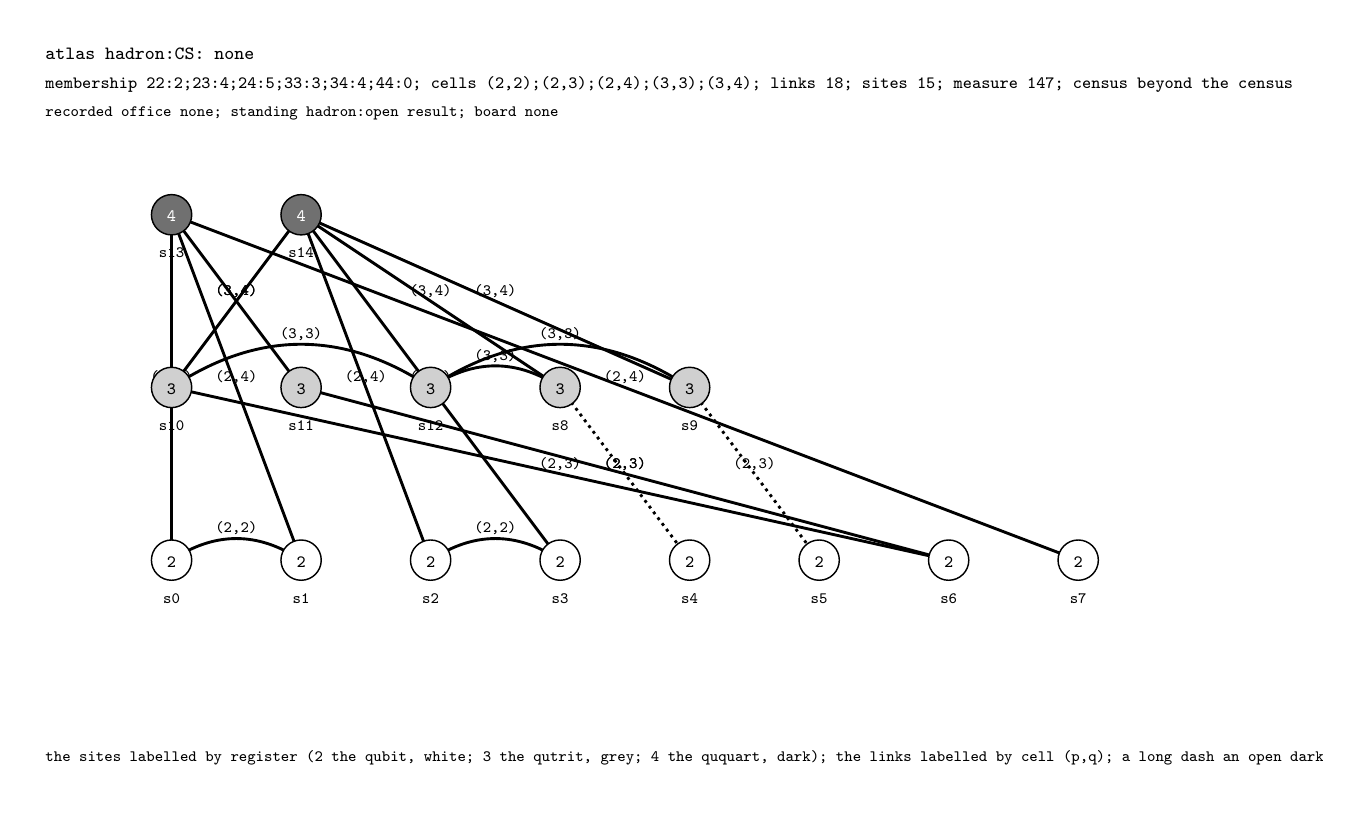
\begin{tikzpicture}[x=0.52pt,y=-0.52pt,baseline]
\clip (0,0) rectangle (900,540);
\fill[white] (0,0) rectangle (900,540);
\node[anchor=base west,inner sep=0pt,text=black,font=\fontsize{6.76}{8.112}\selectfont\ttfamily] at (12,22) {atlas hadron:CS: none};
\node[anchor=base west,inner sep=0pt,text=black,font=\fontsize{6.24}{7.488}\selectfont\ttfamily] at (12,42) {membership 22:2;23:4;24:5;33:3;34:4;44:0; cells (2,2);(2,3);(2,4);(3,3);(3,4); links 18; sites 15; measure 147; census beyond the census};
\node[anchor=base west,inner sep=0pt,text=black,font=\fontsize{5.72}{6.864}\selectfont\ttfamily] at (12,62) {recorded office none; standing hadron:open result; board none};
\draw[draw=black,line width=1.04pt] (100,370) -- (100,130);
\node[anchor=base,inner sep=0pt,text=black,font=\fontsize{5.72}{6.864}\selectfont\ttfamily] at (100,246) {(2,4)};
\draw[draw=black,line width=1.04pt] (100,370) .. controls (130,350) and (160,350) .. (190,370);
\node[anchor=base,inner sep=0pt,text=black,font=\fontsize{5.72}{6.864}\selectfont\ttfamily] at (145,351) {(2,2)};
\draw[draw=black,line width=1.04pt] (190,370) -- (100,130);
\node[anchor=base,inner sep=0pt,text=black,font=\fontsize{5.72}{6.864}\selectfont\ttfamily] at (145,246) {(2,4)};
\draw[draw=black,line width=1.04pt] (100,250) .. controls (160,210) and (220,210) .. (280,250);
\node[anchor=base,inner sep=0pt,text=black,font=\fontsize{5.72}{6.864}\selectfont\ttfamily] at (190,216) {(3,3)};
\draw[draw=black,line width=1.04pt] (100,250) -- (190,130);
\node[anchor=base,inner sep=0pt,text=black,font=\fontsize{5.72}{6.864}\selectfont\ttfamily] at (145,186) {(3,4)};
\draw[draw=black,line width=1.04pt] (100,250) -- (640,370);
\node[anchor=base,inner sep=0pt,text=black,font=\fontsize{5.72}{6.864}\selectfont\ttfamily] at (370,306) {(2,3)};
\draw[draw=black,line width=1.04pt] (190,250) -- (100,130);
\node[anchor=base,inner sep=0pt,text=black,font=\fontsize{5.72}{6.864}\selectfont\ttfamily] at (145,186) {(3,4)};
\draw[draw=black,line width=1.04pt] (190,250) -- (640,370);
\node[anchor=base,inner sep=0pt,text=black,font=\fontsize{5.72}{6.864}\selectfont\ttfamily] at (415,306) {(2,3)};
\draw[draw=black,line width=1.04pt] (280,250) .. controls (310,230) and (340,230) .. (370,250);
\node[anchor=base,inner sep=0pt,text=black,font=\fontsize{5.72}{6.864}\selectfont\ttfamily] at (325,231) {(3,3)};
\draw[draw=black,line width=1.04pt] (280,250) .. controls (340,210) and (400,210) .. (460,250);
\node[anchor=base,inner sep=0pt,text=black,font=\fontsize{5.72}{6.864}\selectfont\ttfamily] at (370,216) {(3,3)};
\draw[draw=black,line width=1.04pt] (100,130) -- (730,370);
\node[anchor=base,inner sep=0pt,text=black,font=\fontsize{5.72}{6.864}\selectfont\ttfamily] at (415,246) {(2,4)};
\draw[draw=black,line width=1.04pt] (190,130) -- (280,370);
\node[anchor=base,inner sep=0pt,text=black,font=\fontsize{5.72}{6.864}\selectfont\ttfamily] at (235,246) {(2,4)};
\draw[draw=black,line width=1.04pt] (190,130) -- (370,370);
\node[anchor=base,inner sep=0pt,text=black,font=\fontsize{5.72}{6.864}\selectfont\ttfamily] at (280,246) {(2,4)};
\draw[draw=black,line width=1.04pt] (190,130) -- (370,250);
\node[anchor=base,inner sep=0pt,text=black,font=\fontsize{5.72}{6.864}\selectfont\ttfamily] at (280,186) {(3,4)};
\draw[draw=black,line width=1.04pt] (190,130) -- (460,250);
\node[anchor=base,inner sep=0pt,text=black,font=\fontsize{5.72}{6.864}\selectfont\ttfamily] at (325,186) {(3,4)};
\draw[draw=black,line width=1.04pt] (280,370) .. controls (310,350) and (340,350) .. (370,370);
\node[anchor=base,inner sep=0pt,text=black,font=\fontsize{5.72}{6.864}\selectfont\ttfamily] at (325,351) {(2,2)};
\draw[draw=black,line width=1.04pt,dash pattern=on 1.04pt off 1.56pt] (460,370) -- (370,250);
\node[anchor=base,inner sep=0pt,text=black,font=\fontsize{5.72}{6.864}\selectfont\ttfamily] at (415,306) {(2,3)};
\draw[draw=black,line width=1.04pt,dash pattern=on 1.04pt off 1.56pt] (550,370) -- (460,250);
\node[anchor=base,inner sep=0pt,text=black,font=\fontsize{5.72}{6.864}\selectfont\ttfamily] at (505,306) {(2,3)};
\filldraw[fill=white,draw=black,line width=0.52pt] (100,370) circle (14);
\node[anchor=base,inner sep=0pt,text=black,font=\fontsize{6.24}{7.488}\selectfont\ttfamily] at (100,375) {2};
\node[anchor=base,inner sep=0pt,text=black,font=\fontsize{5.72}{6.864}\selectfont\ttfamily] at (100,400) {s0};
\filldraw[fill=white,draw=black,line width=0.52pt] (190,370) circle (14);
\node[anchor=base,inner sep=0pt,text=black,font=\fontsize{6.24}{7.488}\selectfont\ttfamily] at (190,375) {2};
\node[anchor=base,inner sep=0pt,text=black,font=\fontsize{5.72}{6.864}\selectfont\ttfamily] at (190,400) {s1};
\filldraw[fill={rgb,255:red,208;green,208;blue,208},draw=black,line width=0.52pt] (100,250) circle (14);
\node[anchor=base,inner sep=0pt,text=black,font=\fontsize{6.24}{7.488}\selectfont\ttfamily] at (100,255) {3};
\node[anchor=base,inner sep=0pt,text=black,font=\fontsize{5.72}{6.864}\selectfont\ttfamily] at (100,280) {s10};
\filldraw[fill={rgb,255:red,208;green,208;blue,208},draw=black,line width=0.52pt] (190,250) circle (14);
\node[anchor=base,inner sep=0pt,text=black,font=\fontsize{6.24}{7.488}\selectfont\ttfamily] at (190,255) {3};
\node[anchor=base,inner sep=0pt,text=black,font=\fontsize{5.72}{6.864}\selectfont\ttfamily] at (190,280) {s11};
\filldraw[fill={rgb,255:red,208;green,208;blue,208},draw=black,line width=0.52pt] (280,250) circle (14);
\node[anchor=base,inner sep=0pt,text=black,font=\fontsize{6.24}{7.488}\selectfont\ttfamily] at (280,255) {3};
\node[anchor=base,inner sep=0pt,text=black,font=\fontsize{5.72}{6.864}\selectfont\ttfamily] at (280,280) {s12};
\filldraw[fill={rgb,255:red,112;green,112;blue,112},draw=black,line width=0.52pt] (100,130) circle (14);
\node[anchor=base,inner sep=0pt,text=white,font=\fontsize{6.24}{7.488}\selectfont\ttfamily] at (100,135) {4};
\node[anchor=base,inner sep=0pt,text=black,font=\fontsize{5.72}{6.864}\selectfont\ttfamily] at (100,160) {s13};
\filldraw[fill={rgb,255:red,112;green,112;blue,112},draw=black,line width=0.52pt] (190,130) circle (14);
\node[anchor=base,inner sep=0pt,text=white,font=\fontsize{6.24}{7.488}\selectfont\ttfamily] at (190,135) {4};
\node[anchor=base,inner sep=0pt,text=black,font=\fontsize{5.72}{6.864}\selectfont\ttfamily] at (190,160) {s14};
\filldraw[fill=white,draw=black,line width=0.52pt] (280,370) circle (14);
\node[anchor=base,inner sep=0pt,text=black,font=\fontsize{6.24}{7.488}\selectfont\ttfamily] at (280,375) {2};
\node[anchor=base,inner sep=0pt,text=black,font=\fontsize{5.72}{6.864}\selectfont\ttfamily] at (280,400) {s2};
\filldraw[fill=white,draw=black,line width=0.52pt] (370,370) circle (14);
\node[anchor=base,inner sep=0pt,text=black,font=\fontsize{6.24}{7.488}\selectfont\ttfamily] at (370,375) {2};
\node[anchor=base,inner sep=0pt,text=black,font=\fontsize{5.72}{6.864}\selectfont\ttfamily] at (370,400) {s3};
\filldraw[fill=white,draw=black,line width=0.52pt] (460,370) circle (14);
\node[anchor=base,inner sep=0pt,text=black,font=\fontsize{6.24}{7.488}\selectfont\ttfamily] at (460,375) {2};
\node[anchor=base,inner sep=0pt,text=black,font=\fontsize{5.72}{6.864}\selectfont\ttfamily] at (460,400) {s4};
\filldraw[fill=white,draw=black,line width=0.52pt] (550,370) circle (14);
\node[anchor=base,inner sep=0pt,text=black,font=\fontsize{6.24}{7.488}\selectfont\ttfamily] at (550,375) {2};
\node[anchor=base,inner sep=0pt,text=black,font=\fontsize{5.72}{6.864}\selectfont\ttfamily] at (550,400) {s5};
\filldraw[fill=white,draw=black,line width=0.52pt] (640,370) circle (14);
\node[anchor=base,inner sep=0pt,text=black,font=\fontsize{6.24}{7.488}\selectfont\ttfamily] at (640,375) {2};
\node[anchor=base,inner sep=0pt,text=black,font=\fontsize{5.72}{6.864}\selectfont\ttfamily] at (640,400) {s6};
\filldraw[fill=white,draw=black,line width=0.52pt] (730,370) circle (14);
\node[anchor=base,inner sep=0pt,text=black,font=\fontsize{6.24}{7.488}\selectfont\ttfamily] at (730,375) {2};
\node[anchor=base,inner sep=0pt,text=black,font=\fontsize{5.72}{6.864}\selectfont\ttfamily] at (730,400) {s7};
\filldraw[fill={rgb,255:red,208;green,208;blue,208},draw=black,line width=0.52pt] (370,250) circle (14);
\node[anchor=base,inner sep=0pt,text=black,font=\fontsize{6.24}{7.488}\selectfont\ttfamily] at (370,255) {3};
\node[anchor=base,inner sep=0pt,text=black,font=\fontsize{5.72}{6.864}\selectfont\ttfamily] at (370,280) {s8};
\filldraw[fill={rgb,255:red,208;green,208;blue,208},draw=black,line width=0.52pt] (460,250) circle (14);
\node[anchor=base,inner sep=0pt,text=black,font=\fontsize{6.24}{7.488}\selectfont\ttfamily] at (460,255) {3};
\node[anchor=base,inner sep=0pt,text=black,font=\fontsize{5.72}{6.864}\selectfont\ttfamily] at (460,280) {s9};
\node[anchor=base west,inner sep=0pt,text=black,font=\fontsize{5.72}{6.864}\selectfont\ttfamily] at (12,510) {the sites labelled by register (2 the qubit, white; 3 the qutrit, grey; 4 the ququart, dark); the links labelled by cell (p,q); a long dash an open dark link of the neutron row; a short dash a docked link at the rule R1};
\end{tikzpicture}\end{adjustbox}
\caption{\texttt{CS of the hadron row}, hadron row body: 15 sites, 18 links, the measure 147; the links at the cells (2,2), (2,3), (2,4), (3,3), (3,4); the membership 22:2; 23:4; 24:5; 33:3; 34:4; 44:0; 2 docked links at the rule R1 (s4-s8; s5-s9); beyond the census of the six cells. Drawn at the anatomy atlas as its web, the sites labeled by register and the links by cell, from the hadron spectroscopy at the cap sinks.}\label{fig:VII-6-D540002-cs-078b31}
\begin{center}\footnotesize\begin{adjustbox}{max width=\linewidth}\begin{tabular}{p{0.26\textwidth}p{0.68\textwidth}}\toprule
recorded office (the slot-count row) & no read of this body at the slot-count row \\
mass register (the mass-register row) & no read of this body at the mass-register row \\
\bottomrule\end{tabular}\end{adjustbox}\end{center}
\end{figure}
\begin{figure}[H]\centering
\begin{adjustbox}{max width=\linewidth}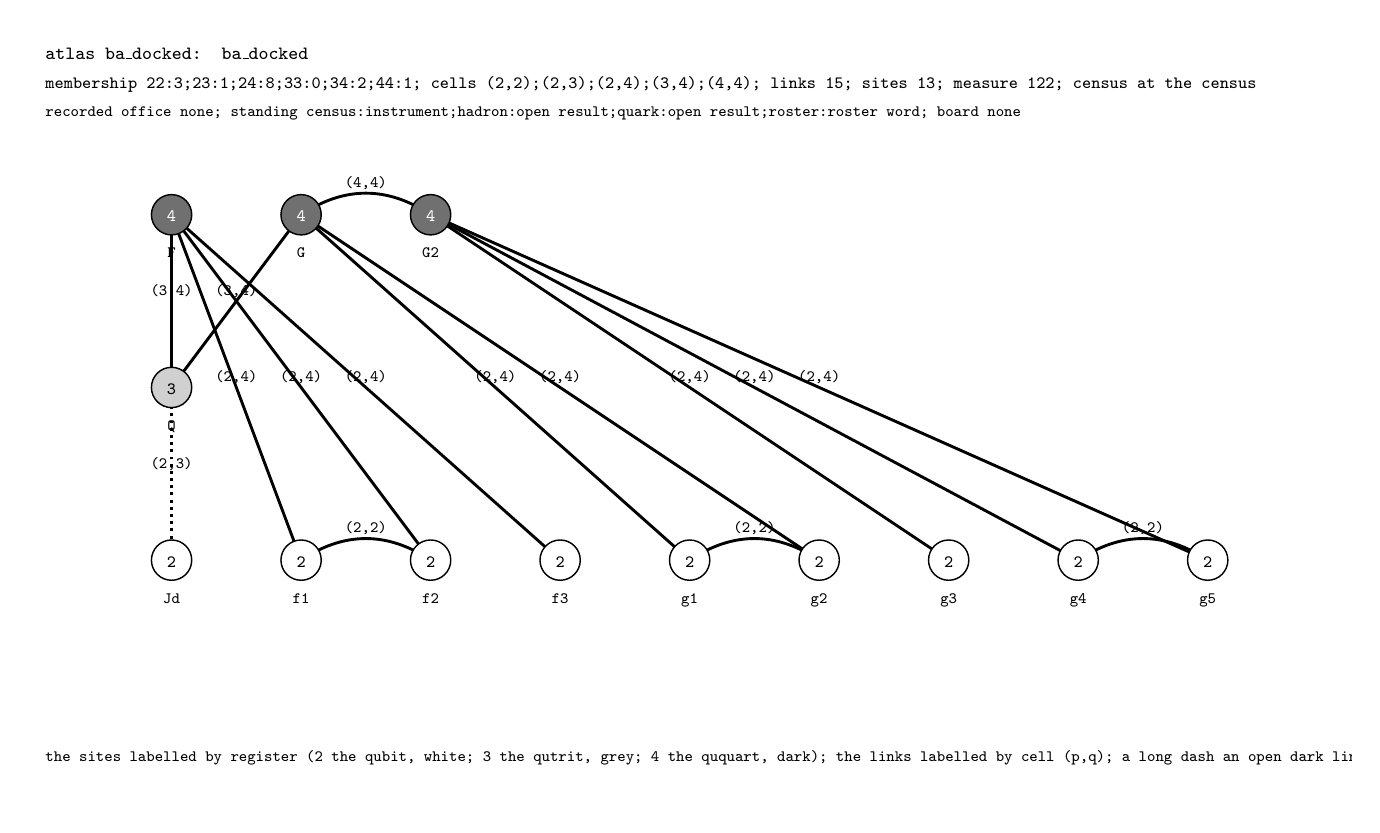
\begin{tikzpicture}[x=0.52pt,y=-0.52pt,baseline]
\clip (0,0) rectangle (920,540);
\fill[white] (0,0) rectangle (920,540);
\node[anchor=base west,inner sep=0pt,text=black,font=\fontsize{6.76}{8.112}\selectfont\ttfamily] at (12,22) {atlas ba\_docked: ba\_docked};
\node[anchor=base west,inner sep=0pt,text=black,font=\fontsize{6.24}{7.488}\selectfont\ttfamily] at (12,42) {membership 22:3;23:1;24:8;33:0;34:2;44:1; cells (2,2);(2,3);(2,4);(3,4);(4,4); links 15; sites 13; measure 122; census at the census};
\node[anchor=base west,inner sep=0pt,text=black,font=\fontsize{5.72}{6.864}\selectfont\ttfamily] at (12,62) {recorded office none; standing census:instrument;hadron:open result;quark:open result;roster:roster word; board none};
\draw[draw=black,line width=1.04pt] (100,130) -- (100,250);
\node[anchor=base,inner sep=0pt,text=black,font=\fontsize{5.72}{6.864}\selectfont\ttfamily] at (100,186) {(3,4)};
\draw[draw=black,line width=1.04pt] (100,130) -- (190,370);
\node[anchor=base,inner sep=0pt,text=black,font=\fontsize{5.72}{6.864}\selectfont\ttfamily] at (145,246) {(2,4)};
\draw[draw=black,line width=1.04pt] (100,130) -- (280,370);
\node[anchor=base,inner sep=0pt,text=black,font=\fontsize{5.72}{6.864}\selectfont\ttfamily] at (190,246) {(2,4)};
\draw[draw=black,line width=1.04pt] (100,130) -- (370,370);
\node[anchor=base,inner sep=0pt,text=black,font=\fontsize{5.72}{6.864}\selectfont\ttfamily] at (235,246) {(2,4)};
\draw[draw=black,line width=1.04pt] (190,130) .. controls (220,110) and (250,110) .. (280,130);
\node[anchor=base,inner sep=0pt,text=black,font=\fontsize{5.72}{6.864}\selectfont\ttfamily] at (235,111) {(4,4)};
\draw[draw=black,line width=1.04pt] (190,130) -- (100,250);
\node[anchor=base,inner sep=0pt,text=black,font=\fontsize{5.72}{6.864}\selectfont\ttfamily] at (145,186) {(3,4)};
\draw[draw=black,line width=1.04pt] (190,130) -- (460,370);
\node[anchor=base,inner sep=0pt,text=black,font=\fontsize{5.72}{6.864}\selectfont\ttfamily] at (325,246) {(2,4)};
\draw[draw=black,line width=1.04pt] (190,130) -- (550,370);
\node[anchor=base,inner sep=0pt,text=black,font=\fontsize{5.72}{6.864}\selectfont\ttfamily] at (370,246) {(2,4)};
\draw[draw=black,line width=1.04pt] (280,130) -- (640,370);
\node[anchor=base,inner sep=0pt,text=black,font=\fontsize{5.72}{6.864}\selectfont\ttfamily] at (460,246) {(2,4)};
\draw[draw=black,line width=1.04pt] (280,130) -- (730,370);
\node[anchor=base,inner sep=0pt,text=black,font=\fontsize{5.72}{6.864}\selectfont\ttfamily] at (505,246) {(2,4)};
\draw[draw=black,line width=1.04pt] (280,130) -- (820,370);
\node[anchor=base,inner sep=0pt,text=black,font=\fontsize{5.72}{6.864}\selectfont\ttfamily] at (550,246) {(2,4)};
\draw[draw=black,line width=1.04pt,dash pattern=on 1.04pt off 1.56pt] (100,370) -- (100,250);
\node[anchor=base,inner sep=0pt,text=black,font=\fontsize{5.72}{6.864}\selectfont\ttfamily] at (100,306) {(2,3)};
\draw[draw=black,line width=1.04pt] (190,370) .. controls (220,350) and (250,350) .. (280,370);
\node[anchor=base,inner sep=0pt,text=black,font=\fontsize{5.72}{6.864}\selectfont\ttfamily] at (235,351) {(2,2)};
\draw[draw=black,line width=1.04pt] (460,370) .. controls (490,350) and (520,350) .. (550,370);
\node[anchor=base,inner sep=0pt,text=black,font=\fontsize{5.72}{6.864}\selectfont\ttfamily] at (505,351) {(2,2)};
\draw[draw=black,line width=1.04pt] (730,370) .. controls (760,350) and (790,350) .. (820,370);
\node[anchor=base,inner sep=0pt,text=black,font=\fontsize{5.72}{6.864}\selectfont\ttfamily] at (775,351) {(2,2)};
\filldraw[fill={rgb,255:red,112;green,112;blue,112},draw=black,line width=0.52pt] (100,130) circle (14);
\node[anchor=base,inner sep=0pt,text=white,font=\fontsize{6.24}{7.488}\selectfont\ttfamily] at (100,135) {4};
\node[anchor=base,inner sep=0pt,text=black,font=\fontsize{5.72}{6.864}\selectfont\ttfamily] at (100,160) {F};
\filldraw[fill={rgb,255:red,112;green,112;blue,112},draw=black,line width=0.52pt] (190,130) circle (14);
\node[anchor=base,inner sep=0pt,text=white,font=\fontsize{6.24}{7.488}\selectfont\ttfamily] at (190,135) {4};
\node[anchor=base,inner sep=0pt,text=black,font=\fontsize{5.72}{6.864}\selectfont\ttfamily] at (190,160) {G};
\filldraw[fill={rgb,255:red,112;green,112;blue,112},draw=black,line width=0.52pt] (280,130) circle (14);
\node[anchor=base,inner sep=0pt,text=white,font=\fontsize{6.24}{7.488}\selectfont\ttfamily] at (280,135) {4};
\node[anchor=base,inner sep=0pt,text=black,font=\fontsize{5.72}{6.864}\selectfont\ttfamily] at (280,160) {G2};
\filldraw[fill=white,draw=black,line width=0.52pt] (100,370) circle (14);
\node[anchor=base,inner sep=0pt,text=black,font=\fontsize{6.24}{7.488}\selectfont\ttfamily] at (100,375) {2};
\node[anchor=base,inner sep=0pt,text=black,font=\fontsize{5.72}{6.864}\selectfont\ttfamily] at (100,400) {Jd};
\filldraw[fill={rgb,255:red,208;green,208;blue,208},draw=black,line width=0.52pt] (100,250) circle (14);
\node[anchor=base,inner sep=0pt,text=black,font=\fontsize{6.24}{7.488}\selectfont\ttfamily] at (100,255) {3};
\node[anchor=base,inner sep=0pt,text=black,font=\fontsize{5.72}{6.864}\selectfont\ttfamily] at (100,280) {Q};
\filldraw[fill=white,draw=black,line width=0.52pt] (190,370) circle (14);
\node[anchor=base,inner sep=0pt,text=black,font=\fontsize{6.24}{7.488}\selectfont\ttfamily] at (190,375) {2};
\node[anchor=base,inner sep=0pt,text=black,font=\fontsize{5.72}{6.864}\selectfont\ttfamily] at (190,400) {f1};
\filldraw[fill=white,draw=black,line width=0.52pt] (280,370) circle (14);
\node[anchor=base,inner sep=0pt,text=black,font=\fontsize{6.24}{7.488}\selectfont\ttfamily] at (280,375) {2};
\node[anchor=base,inner sep=0pt,text=black,font=\fontsize{5.72}{6.864}\selectfont\ttfamily] at (280,400) {f2};
\filldraw[fill=white,draw=black,line width=0.52pt] (370,370) circle (14);
\node[anchor=base,inner sep=0pt,text=black,font=\fontsize{6.24}{7.488}\selectfont\ttfamily] at (370,375) {2};
\node[anchor=base,inner sep=0pt,text=black,font=\fontsize{5.72}{6.864}\selectfont\ttfamily] at (370,400) {f3};
\filldraw[fill=white,draw=black,line width=0.52pt] (460,370) circle (14);
\node[anchor=base,inner sep=0pt,text=black,font=\fontsize{6.24}{7.488}\selectfont\ttfamily] at (460,375) {2};
\node[anchor=base,inner sep=0pt,text=black,font=\fontsize{5.72}{6.864}\selectfont\ttfamily] at (460,400) {g1};
\filldraw[fill=white,draw=black,line width=0.52pt] (550,370) circle (14);
\node[anchor=base,inner sep=0pt,text=black,font=\fontsize{6.24}{7.488}\selectfont\ttfamily] at (550,375) {2};
\node[anchor=base,inner sep=0pt,text=black,font=\fontsize{5.72}{6.864}\selectfont\ttfamily] at (550,400) {g2};
\filldraw[fill=white,draw=black,line width=0.52pt] (640,370) circle (14);
\node[anchor=base,inner sep=0pt,text=black,font=\fontsize{6.24}{7.488}\selectfont\ttfamily] at (640,375) {2};
\node[anchor=base,inner sep=0pt,text=black,font=\fontsize{5.72}{6.864}\selectfont\ttfamily] at (640,400) {g3};
\filldraw[fill=white,draw=black,line width=0.52pt] (730,370) circle (14);
\node[anchor=base,inner sep=0pt,text=black,font=\fontsize{6.24}{7.488}\selectfont\ttfamily] at (730,375) {2};
\node[anchor=base,inner sep=0pt,text=black,font=\fontsize{5.72}{6.864}\selectfont\ttfamily] at (730,400) {g4};
\filldraw[fill=white,draw=black,line width=0.52pt] (820,370) circle (14);
\node[anchor=base,inner sep=0pt,text=black,font=\fontsize{6.24}{7.488}\selectfont\ttfamily] at (820,375) {2};
\node[anchor=base,inner sep=0pt,text=black,font=\fontsize{5.72}{6.864}\selectfont\ttfamily] at (820,400) {g5};
\node[anchor=base west,inner sep=0pt,text=black,font=\fontsize{5.72}{6.864}\selectfont\ttfamily] at (12,510) {the sites labelled by register (2 the qubit, white; 3 the qutrit, grey; 4 the ququart, dark); the links labelled by cell (p,q); a long dash an open dark link of the neutron row; a short dash a docked link at the rule R1};
\end{tikzpicture}\end{adjustbox}
\caption{\texttt{ba\_docked}, hadron row body: 13 sites, 15 links, the measure 122; the links at the cells (2,2), (2,3), (2,4), (3,4), (4,4); the membership 22:3; 23:1; 24:8; 33:0; 34:2; 44:1; 1 docked links at the rule R1 (Q-Jd); at the census of the six cells. Drawn at the anatomy atlas as its web, the sites labeled by register and the links by cell, from the hadron spectroscopy at the cap sinks.}\label{fig:VII-6-D540002-ba-docked-7309c8}
\begin{center}\footnotesize\begin{adjustbox}{max width=\linewidth}\begin{tabular}{p{0.26\textwidth}p{0.68\textwidth}}\toprule
recorded office (the slot-count row) & no read of this body at the slot-count row \\
mass register (the mass-register row) & the read kba: the class touching the ququart; the first power 1044; the office \texttt{5 022 456 423 459 713/4608000000\textbar{}219/50\textbar{}5069/2304000\textbar{}0}; nonzero; met yes; hubs F; G; G2; in-legs q-f; q-g; dressing 9; ports F-f3; G2-g3; Q-Jd \\
\bottomrule\end{tabular}\end{adjustbox}\end{center}
\end{figure}
\begin{figure}[H]\centering
\begin{adjustbox}{max width=\linewidth}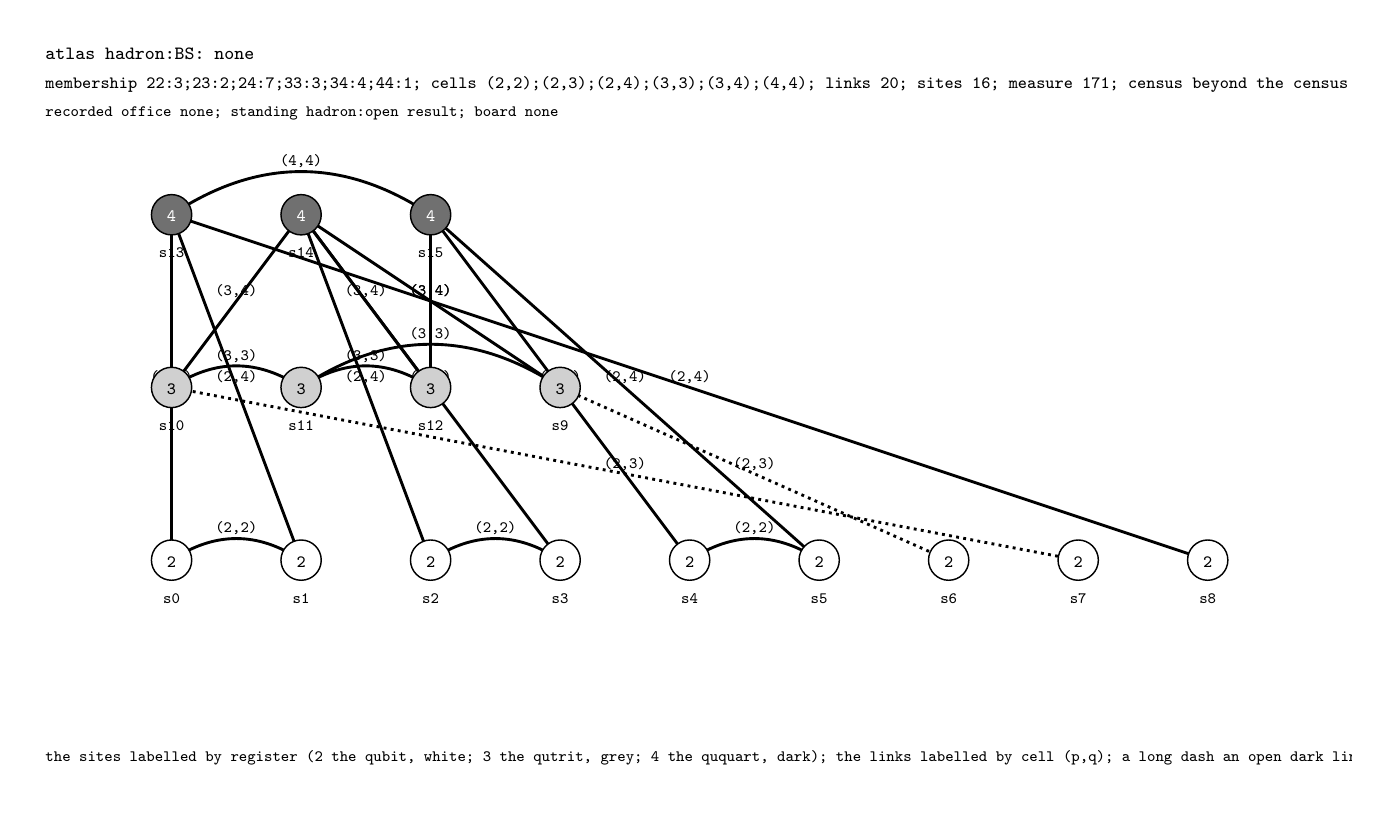
\begin{tikzpicture}[x=0.52pt,y=-0.52pt,baseline]
\clip (0,0) rectangle (920,540);
\fill[white] (0,0) rectangle (920,540);
\node[anchor=base west,inner sep=0pt,text=black,font=\fontsize{6.76}{8.112}\selectfont\ttfamily] at (12,22) {atlas hadron:BS: none};
\node[anchor=base west,inner sep=0pt,text=black,font=\fontsize{6.24}{7.488}\selectfont\ttfamily] at (12,42) {membership 22:3;23:2;24:7;33:3;34:4;44:1; cells (2,2);(2,3);(2,4);(3,3);(3,4);(4,4); links 20; sites 16; measure 171; census beyond the census};
\node[anchor=base west,inner sep=0pt,text=black,font=\fontsize{5.72}{6.864}\selectfont\ttfamily] at (12,62) {recorded office none; standing hadron:open result; board none};
\draw[draw=black,line width=1.04pt] (100,370) -- (100,130);
\node[anchor=base,inner sep=0pt,text=black,font=\fontsize{5.72}{6.864}\selectfont\ttfamily] at (100,246) {(2,4)};
\draw[draw=black,line width=1.04pt] (100,370) .. controls (130,350) and (160,350) .. (190,370);
\node[anchor=base,inner sep=0pt,text=black,font=\fontsize{5.72}{6.864}\selectfont\ttfamily] at (145,351) {(2,2)};
\draw[draw=black,line width=1.04pt] (190,370) -- (100,130);
\node[anchor=base,inner sep=0pt,text=black,font=\fontsize{5.72}{6.864}\selectfont\ttfamily] at (145,246) {(2,4)};
\draw[draw=black,line width=1.04pt] (100,250) .. controls (130,230) and (160,230) .. (190,250);
\node[anchor=base,inner sep=0pt,text=black,font=\fontsize{5.72}{6.864}\selectfont\ttfamily] at (145,231) {(3,3)};
\draw[draw=black,line width=1.04pt] (100,250) -- (190,130);
\node[anchor=base,inner sep=0pt,text=black,font=\fontsize{5.72}{6.864}\selectfont\ttfamily] at (145,186) {(3,4)};
\draw[draw=black,line width=1.04pt,dash pattern=on 1.04pt off 1.56pt] (100,250) -- (730,370);
\node[anchor=base,inner sep=0pt,text=black,font=\fontsize{5.72}{6.864}\selectfont\ttfamily] at (415,306) {(2,3)};
\draw[draw=black,line width=1.04pt] (190,250) .. controls (220,230) and (250,230) .. (280,250);
\node[anchor=base,inner sep=0pt,text=black,font=\fontsize{5.72}{6.864}\selectfont\ttfamily] at (235,231) {(3,3)};
\draw[draw=black,line width=1.04pt] (190,250) .. controls (250,210) and (310,210) .. (370,250);
\node[anchor=base,inner sep=0pt,text=black,font=\fontsize{5.72}{6.864}\selectfont\ttfamily] at (280,216) {(3,3)};
\draw[draw=black,line width=1.04pt] (280,250) -- (190,130);
\node[anchor=base,inner sep=0pt,text=black,font=\fontsize{5.72}{6.864}\selectfont\ttfamily] at (235,186) {(3,4)};
\draw[draw=black,line width=1.04pt] (280,250) -- (280,130);
\node[anchor=base,inner sep=0pt,text=black,font=\fontsize{5.72}{6.864}\selectfont\ttfamily] at (280,186) {(3,4)};
\draw[draw=black,line width=1.04pt] (100,130) .. controls (160,90) and (220,90) .. (280,130);
\node[anchor=base,inner sep=0pt,text=black,font=\fontsize{5.72}{6.864}\selectfont\ttfamily] at (190,96) {(4,4)};
\draw[draw=black,line width=1.04pt] (100,130) -- (820,370);
\node[anchor=base,inner sep=0pt,text=black,font=\fontsize{5.72}{6.864}\selectfont\ttfamily] at (460,246) {(2,4)};
\draw[draw=black,line width=1.04pt] (190,130) -- (280,370);
\node[anchor=base,inner sep=0pt,text=black,font=\fontsize{5.72}{6.864}\selectfont\ttfamily] at (235,246) {(2,4)};
\draw[draw=black,line width=1.04pt] (190,130) -- (370,370);
\node[anchor=base,inner sep=0pt,text=black,font=\fontsize{5.72}{6.864}\selectfont\ttfamily] at (280,246) {(2,4)};
\draw[draw=black,line width=1.04pt] (190,130) -- (370,250);
\node[anchor=base,inner sep=0pt,text=black,font=\fontsize{5.72}{6.864}\selectfont\ttfamily] at (280,186) {(3,4)};
\draw[draw=black,line width=1.04pt] (280,130) -- (460,370);
\node[anchor=base,inner sep=0pt,text=black,font=\fontsize{5.72}{6.864}\selectfont\ttfamily] at (370,246) {(2,4)};
\draw[draw=black,line width=1.04pt] (280,130) -- (550,370);
\node[anchor=base,inner sep=0pt,text=black,font=\fontsize{5.72}{6.864}\selectfont\ttfamily] at (415,246) {(2,4)};
\draw[draw=black,line width=1.04pt] (280,370) .. controls (310,350) and (340,350) .. (370,370);
\node[anchor=base,inner sep=0pt,text=black,font=\fontsize{5.72}{6.864}\selectfont\ttfamily] at (325,351) {(2,2)};
\draw[draw=black,line width=1.04pt] (460,370) .. controls (490,350) and (520,350) .. (550,370);
\node[anchor=base,inner sep=0pt,text=black,font=\fontsize{5.72}{6.864}\selectfont\ttfamily] at (505,351) {(2,2)};
\draw[draw=black,line width=1.04pt,dash pattern=on 1.04pt off 1.56pt] (640,370) -- (370,250);
\node[anchor=base,inner sep=0pt,text=black,font=\fontsize{5.72}{6.864}\selectfont\ttfamily] at (505,306) {(2,3)};
\filldraw[fill=white,draw=black,line width=0.52pt] (100,370) circle (14);
\node[anchor=base,inner sep=0pt,text=black,font=\fontsize{6.24}{7.488}\selectfont\ttfamily] at (100,375) {2};
\node[anchor=base,inner sep=0pt,text=black,font=\fontsize{5.72}{6.864}\selectfont\ttfamily] at (100,400) {s0};
\filldraw[fill=white,draw=black,line width=0.52pt] (190,370) circle (14);
\node[anchor=base,inner sep=0pt,text=black,font=\fontsize{6.24}{7.488}\selectfont\ttfamily] at (190,375) {2};
\node[anchor=base,inner sep=0pt,text=black,font=\fontsize{5.72}{6.864}\selectfont\ttfamily] at (190,400) {s1};
\filldraw[fill={rgb,255:red,208;green,208;blue,208},draw=black,line width=0.52pt] (100,250) circle (14);
\node[anchor=base,inner sep=0pt,text=black,font=\fontsize{6.24}{7.488}\selectfont\ttfamily] at (100,255) {3};
\node[anchor=base,inner sep=0pt,text=black,font=\fontsize{5.72}{6.864}\selectfont\ttfamily] at (100,280) {s10};
\filldraw[fill={rgb,255:red,208;green,208;blue,208},draw=black,line width=0.52pt] (190,250) circle (14);
\node[anchor=base,inner sep=0pt,text=black,font=\fontsize{6.24}{7.488}\selectfont\ttfamily] at (190,255) {3};
\node[anchor=base,inner sep=0pt,text=black,font=\fontsize{5.72}{6.864}\selectfont\ttfamily] at (190,280) {s11};
\filldraw[fill={rgb,255:red,208;green,208;blue,208},draw=black,line width=0.52pt] (280,250) circle (14);
\node[anchor=base,inner sep=0pt,text=black,font=\fontsize{6.24}{7.488}\selectfont\ttfamily] at (280,255) {3};
\node[anchor=base,inner sep=0pt,text=black,font=\fontsize{5.72}{6.864}\selectfont\ttfamily] at (280,280) {s12};
\filldraw[fill={rgb,255:red,112;green,112;blue,112},draw=black,line width=0.52pt] (100,130) circle (14);
\node[anchor=base,inner sep=0pt,text=white,font=\fontsize{6.24}{7.488}\selectfont\ttfamily] at (100,135) {4};
\node[anchor=base,inner sep=0pt,text=black,font=\fontsize{5.72}{6.864}\selectfont\ttfamily] at (100,160) {s13};
\filldraw[fill={rgb,255:red,112;green,112;blue,112},draw=black,line width=0.52pt] (190,130) circle (14);
\node[anchor=base,inner sep=0pt,text=white,font=\fontsize{6.24}{7.488}\selectfont\ttfamily] at (190,135) {4};
\node[anchor=base,inner sep=0pt,text=black,font=\fontsize{5.72}{6.864}\selectfont\ttfamily] at (190,160) {s14};
\filldraw[fill={rgb,255:red,112;green,112;blue,112},draw=black,line width=0.52pt] (280,130) circle (14);
\node[anchor=base,inner sep=0pt,text=white,font=\fontsize{6.24}{7.488}\selectfont\ttfamily] at (280,135) {4};
\node[anchor=base,inner sep=0pt,text=black,font=\fontsize{5.72}{6.864}\selectfont\ttfamily] at (280,160) {s15};
\filldraw[fill=white,draw=black,line width=0.52pt] (280,370) circle (14);
\node[anchor=base,inner sep=0pt,text=black,font=\fontsize{6.24}{7.488}\selectfont\ttfamily] at (280,375) {2};
\node[anchor=base,inner sep=0pt,text=black,font=\fontsize{5.72}{6.864}\selectfont\ttfamily] at (280,400) {s2};
\filldraw[fill=white,draw=black,line width=0.52pt] (370,370) circle (14);
\node[anchor=base,inner sep=0pt,text=black,font=\fontsize{6.24}{7.488}\selectfont\ttfamily] at (370,375) {2};
\node[anchor=base,inner sep=0pt,text=black,font=\fontsize{5.72}{6.864}\selectfont\ttfamily] at (370,400) {s3};
\filldraw[fill=white,draw=black,line width=0.52pt] (460,370) circle (14);
\node[anchor=base,inner sep=0pt,text=black,font=\fontsize{6.24}{7.488}\selectfont\ttfamily] at (460,375) {2};
\node[anchor=base,inner sep=0pt,text=black,font=\fontsize{5.72}{6.864}\selectfont\ttfamily] at (460,400) {s4};
\filldraw[fill=white,draw=black,line width=0.52pt] (550,370) circle (14);
\node[anchor=base,inner sep=0pt,text=black,font=\fontsize{6.24}{7.488}\selectfont\ttfamily] at (550,375) {2};
\node[anchor=base,inner sep=0pt,text=black,font=\fontsize{5.72}{6.864}\selectfont\ttfamily] at (550,400) {s5};
\filldraw[fill=white,draw=black,line width=0.52pt] (640,370) circle (14);
\node[anchor=base,inner sep=0pt,text=black,font=\fontsize{6.24}{7.488}\selectfont\ttfamily] at (640,375) {2};
\node[anchor=base,inner sep=0pt,text=black,font=\fontsize{5.72}{6.864}\selectfont\ttfamily] at (640,400) {s6};
\filldraw[fill=white,draw=black,line width=0.52pt] (730,370) circle (14);
\node[anchor=base,inner sep=0pt,text=black,font=\fontsize{6.24}{7.488}\selectfont\ttfamily] at (730,375) {2};
\node[anchor=base,inner sep=0pt,text=black,font=\fontsize{5.72}{6.864}\selectfont\ttfamily] at (730,400) {s7};
\filldraw[fill=white,draw=black,line width=0.52pt] (820,370) circle (14);
\node[anchor=base,inner sep=0pt,text=black,font=\fontsize{6.24}{7.488}\selectfont\ttfamily] at (820,375) {2};
\node[anchor=base,inner sep=0pt,text=black,font=\fontsize{5.72}{6.864}\selectfont\ttfamily] at (820,400) {s8};
\filldraw[fill={rgb,255:red,208;green,208;blue,208},draw=black,line width=0.52pt] (370,250) circle (14);
\node[anchor=base,inner sep=0pt,text=black,font=\fontsize{6.24}{7.488}\selectfont\ttfamily] at (370,255) {3};
\node[anchor=base,inner sep=0pt,text=black,font=\fontsize{5.72}{6.864}\selectfont\ttfamily] at (370,280) {s9};
\node[anchor=base west,inner sep=0pt,text=black,font=\fontsize{5.72}{6.864}\selectfont\ttfamily] at (12,510) {the sites labelled by register (2 the qubit, white; 3 the qutrit, grey; 4 the ququart, dark); the links labelled by cell (p,q); a long dash an open dark link of the neutron row; a short dash a docked link at the rule R1};
\end{tikzpicture}\end{adjustbox}
\caption{\texttt{BS of the hadron row}, hadron row body: 16 sites, 20 links, the measure 171; the links at the cells (2,2), (2,3), (2,4), (3,3), (3,4), (4,4); the membership 22:3; 23:2; 24:7; 33:3; 34:4; 44:1; 2 docked links at the rule R1 (s6-s9; s7-s10); beyond the census of the six cells. Drawn at the anatomy atlas as its web, the sites labeled by register and the links by cell, from the hadron spectroscopy at the cap sinks.}\label{fig:VII-6-D540002-bs-dfdd5c}
\begin{center}\footnotesize\begin{adjustbox}{max width=\linewidth}\begin{tabular}{p{0.26\textwidth}p{0.68\textwidth}}\toprule
recorded office (the slot-count row) & no read of this body at the slot-count row \\
mass register (the mass-register row) & no read of this body at the mass-register row \\
\bottomrule\end{tabular}\end{adjustbox}\end{center}
\end{figure}
\begin{figure}[H]\centering
\begin{adjustbox}{max width=\linewidth}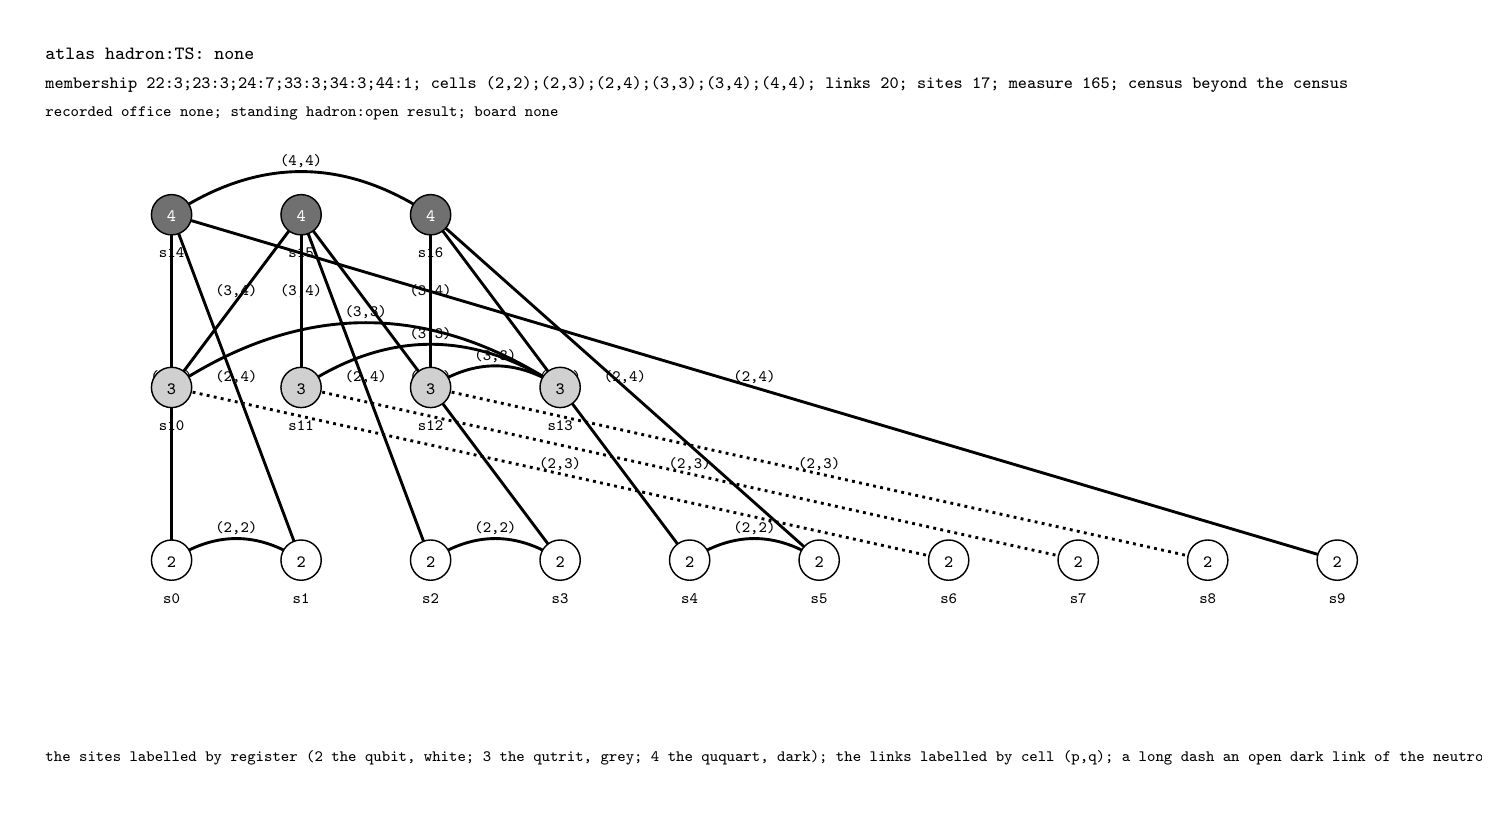
\begin{tikzpicture}[x=0.52pt,y=-0.52pt,baseline]
\clip (0,0) rectangle (1010,540);
\fill[white] (0,0) rectangle (1010,540);
\node[anchor=base west,inner sep=0pt,text=black,font=\fontsize{6.76}{8.112}\selectfont\ttfamily] at (12,22) {atlas hadron:TS: none};
\node[anchor=base west,inner sep=0pt,text=black,font=\fontsize{6.24}{7.488}\selectfont\ttfamily] at (12,42) {membership 22:3;23:3;24:7;33:3;34:3;44:1; cells (2,2);(2,3);(2,4);(3,3);(3,4);(4,4); links 20; sites 17; measure 165; census beyond the census};
\node[anchor=base west,inner sep=0pt,text=black,font=\fontsize{5.72}{6.864}\selectfont\ttfamily] at (12,62) {recorded office none; standing hadron:open result; board none};
\draw[draw=black,line width=1.04pt] (100,370) -- (100,130);
\node[anchor=base,inner sep=0pt,text=black,font=\fontsize{5.72}{6.864}\selectfont\ttfamily] at (100,246) {(2,4)};
\draw[draw=black,line width=1.04pt] (100,370) .. controls (130,350) and (160,350) .. (190,370);
\node[anchor=base,inner sep=0pt,text=black,font=\fontsize{5.72}{6.864}\selectfont\ttfamily] at (145,351) {(2,2)};
\draw[draw=black,line width=1.04pt] (190,370) -- (100,130);
\node[anchor=base,inner sep=0pt,text=black,font=\fontsize{5.72}{6.864}\selectfont\ttfamily] at (145,246) {(2,4)};
\draw[draw=black,line width=1.04pt] (100,250) .. controls (190,190) and (280,190) .. (370,250);
\node[anchor=base,inner sep=0pt,text=black,font=\fontsize{5.72}{6.864}\selectfont\ttfamily] at (235,201) {(3,3)};
\draw[draw=black,line width=1.04pt] (100,250) -- (190,130);
\node[anchor=base,inner sep=0pt,text=black,font=\fontsize{5.72}{6.864}\selectfont\ttfamily] at (145,186) {(3,4)};
\draw[draw=black,line width=1.04pt,dash pattern=on 1.04pt off 1.56pt] (100,250) -- (640,370);
\node[anchor=base,inner sep=0pt,text=black,font=\fontsize{5.72}{6.864}\selectfont\ttfamily] at (370,306) {(2,3)};
\draw[draw=black,line width=1.04pt] (190,250) .. controls (250,210) and (310,210) .. (370,250);
\node[anchor=base,inner sep=0pt,text=black,font=\fontsize{5.72}{6.864}\selectfont\ttfamily] at (280,216) {(3,3)};
\draw[draw=black,line width=1.04pt] (190,250) -- (190,130);
\node[anchor=base,inner sep=0pt,text=black,font=\fontsize{5.72}{6.864}\selectfont\ttfamily] at (190,186) {(3,4)};
\draw[draw=black,line width=1.04pt,dash pattern=on 1.04pt off 1.56pt] (190,250) -- (730,370);
\node[anchor=base,inner sep=0pt,text=black,font=\fontsize{5.72}{6.864}\selectfont\ttfamily] at (460,306) {(2,3)};
\draw[draw=black,line width=1.04pt] (280,250) .. controls (310,230) and (340,230) .. (370,250);
\node[anchor=base,inner sep=0pt,text=black,font=\fontsize{5.72}{6.864}\selectfont\ttfamily] at (325,231) {(3,3)};
\draw[draw=black,line width=1.04pt] (280,250) -- (280,130);
\node[anchor=base,inner sep=0pt,text=black,font=\fontsize{5.72}{6.864}\selectfont\ttfamily] at (280,186) {(3,4)};
\draw[draw=black,line width=1.04pt,dash pattern=on 1.04pt off 1.56pt] (280,250) -- (820,370);
\node[anchor=base,inner sep=0pt,text=black,font=\fontsize{5.72}{6.864}\selectfont\ttfamily] at (550,306) {(2,3)};
\draw[draw=black,line width=1.04pt] (100,130) .. controls (160,90) and (220,90) .. (280,130);
\node[anchor=base,inner sep=0pt,text=black,font=\fontsize{5.72}{6.864}\selectfont\ttfamily] at (190,96) {(4,4)};
\draw[draw=black,line width=1.04pt] (100,130) -- (910,370);
\node[anchor=base,inner sep=0pt,text=black,font=\fontsize{5.72}{6.864}\selectfont\ttfamily] at (505,246) {(2,4)};
\draw[draw=black,line width=1.04pt] (190,130) -- (280,370);
\node[anchor=base,inner sep=0pt,text=black,font=\fontsize{5.72}{6.864}\selectfont\ttfamily] at (235,246) {(2,4)};
\draw[draw=black,line width=1.04pt] (190,130) -- (370,370);
\node[anchor=base,inner sep=0pt,text=black,font=\fontsize{5.72}{6.864}\selectfont\ttfamily] at (280,246) {(2,4)};
\draw[draw=black,line width=1.04pt] (280,130) -- (460,370);
\node[anchor=base,inner sep=0pt,text=black,font=\fontsize{5.72}{6.864}\selectfont\ttfamily] at (370,246) {(2,4)};
\draw[draw=black,line width=1.04pt] (280,130) -- (550,370);
\node[anchor=base,inner sep=0pt,text=black,font=\fontsize{5.72}{6.864}\selectfont\ttfamily] at (415,246) {(2,4)};
\draw[draw=black,line width=1.04pt] (280,370) .. controls (310,350) and (340,350) .. (370,370);
\node[anchor=base,inner sep=0pt,text=black,font=\fontsize{5.72}{6.864}\selectfont\ttfamily] at (325,351) {(2,2)};
\draw[draw=black,line width=1.04pt] (460,370) .. controls (490,350) and (520,350) .. (550,370);
\node[anchor=base,inner sep=0pt,text=black,font=\fontsize{5.72}{6.864}\selectfont\ttfamily] at (505,351) {(2,2)};
\filldraw[fill=white,draw=black,line width=0.52pt] (100,370) circle (14);
\node[anchor=base,inner sep=0pt,text=black,font=\fontsize{6.24}{7.488}\selectfont\ttfamily] at (100,375) {2};
\node[anchor=base,inner sep=0pt,text=black,font=\fontsize{5.72}{6.864}\selectfont\ttfamily] at (100,400) {s0};
\filldraw[fill=white,draw=black,line width=0.52pt] (190,370) circle (14);
\node[anchor=base,inner sep=0pt,text=black,font=\fontsize{6.24}{7.488}\selectfont\ttfamily] at (190,375) {2};
\node[anchor=base,inner sep=0pt,text=black,font=\fontsize{5.72}{6.864}\selectfont\ttfamily] at (190,400) {s1};
\filldraw[fill={rgb,255:red,208;green,208;blue,208},draw=black,line width=0.52pt] (100,250) circle (14);
\node[anchor=base,inner sep=0pt,text=black,font=\fontsize{6.24}{7.488}\selectfont\ttfamily] at (100,255) {3};
\node[anchor=base,inner sep=0pt,text=black,font=\fontsize{5.72}{6.864}\selectfont\ttfamily] at (100,280) {s10};
\filldraw[fill={rgb,255:red,208;green,208;blue,208},draw=black,line width=0.52pt] (190,250) circle (14);
\node[anchor=base,inner sep=0pt,text=black,font=\fontsize{6.24}{7.488}\selectfont\ttfamily] at (190,255) {3};
\node[anchor=base,inner sep=0pt,text=black,font=\fontsize{5.72}{6.864}\selectfont\ttfamily] at (190,280) {s11};
\filldraw[fill={rgb,255:red,208;green,208;blue,208},draw=black,line width=0.52pt] (280,250) circle (14);
\node[anchor=base,inner sep=0pt,text=black,font=\fontsize{6.24}{7.488}\selectfont\ttfamily] at (280,255) {3};
\node[anchor=base,inner sep=0pt,text=black,font=\fontsize{5.72}{6.864}\selectfont\ttfamily] at (280,280) {s12};
\filldraw[fill={rgb,255:red,208;green,208;blue,208},draw=black,line width=0.52pt] (370,250) circle (14);
\node[anchor=base,inner sep=0pt,text=black,font=\fontsize{6.24}{7.488}\selectfont\ttfamily] at (370,255) {3};
\node[anchor=base,inner sep=0pt,text=black,font=\fontsize{5.72}{6.864}\selectfont\ttfamily] at (370,280) {s13};
\filldraw[fill={rgb,255:red,112;green,112;blue,112},draw=black,line width=0.52pt] (100,130) circle (14);
\node[anchor=base,inner sep=0pt,text=white,font=\fontsize{6.24}{7.488}\selectfont\ttfamily] at (100,135) {4};
\node[anchor=base,inner sep=0pt,text=black,font=\fontsize{5.72}{6.864}\selectfont\ttfamily] at (100,160) {s14};
\filldraw[fill={rgb,255:red,112;green,112;blue,112},draw=black,line width=0.52pt] (190,130) circle (14);
\node[anchor=base,inner sep=0pt,text=white,font=\fontsize{6.24}{7.488}\selectfont\ttfamily] at (190,135) {4};
\node[anchor=base,inner sep=0pt,text=black,font=\fontsize{5.72}{6.864}\selectfont\ttfamily] at (190,160) {s15};
\filldraw[fill={rgb,255:red,112;green,112;blue,112},draw=black,line width=0.52pt] (280,130) circle (14);
\node[anchor=base,inner sep=0pt,text=white,font=\fontsize{6.24}{7.488}\selectfont\ttfamily] at (280,135) {4};
\node[anchor=base,inner sep=0pt,text=black,font=\fontsize{5.72}{6.864}\selectfont\ttfamily] at (280,160) {s16};
\filldraw[fill=white,draw=black,line width=0.52pt] (280,370) circle (14);
\node[anchor=base,inner sep=0pt,text=black,font=\fontsize{6.24}{7.488}\selectfont\ttfamily] at (280,375) {2};
\node[anchor=base,inner sep=0pt,text=black,font=\fontsize{5.72}{6.864}\selectfont\ttfamily] at (280,400) {s2};
\filldraw[fill=white,draw=black,line width=0.52pt] (370,370) circle (14);
\node[anchor=base,inner sep=0pt,text=black,font=\fontsize{6.24}{7.488}\selectfont\ttfamily] at (370,375) {2};
\node[anchor=base,inner sep=0pt,text=black,font=\fontsize{5.72}{6.864}\selectfont\ttfamily] at (370,400) {s3};
\filldraw[fill=white,draw=black,line width=0.52pt] (460,370) circle (14);
\node[anchor=base,inner sep=0pt,text=black,font=\fontsize{6.24}{7.488}\selectfont\ttfamily] at (460,375) {2};
\node[anchor=base,inner sep=0pt,text=black,font=\fontsize{5.72}{6.864}\selectfont\ttfamily] at (460,400) {s4};
\filldraw[fill=white,draw=black,line width=0.52pt] (550,370) circle (14);
\node[anchor=base,inner sep=0pt,text=black,font=\fontsize{6.24}{7.488}\selectfont\ttfamily] at (550,375) {2};
\node[anchor=base,inner sep=0pt,text=black,font=\fontsize{5.72}{6.864}\selectfont\ttfamily] at (550,400) {s5};
\filldraw[fill=white,draw=black,line width=0.52pt] (640,370) circle (14);
\node[anchor=base,inner sep=0pt,text=black,font=\fontsize{6.24}{7.488}\selectfont\ttfamily] at (640,375) {2};
\node[anchor=base,inner sep=0pt,text=black,font=\fontsize{5.72}{6.864}\selectfont\ttfamily] at (640,400) {s6};
\filldraw[fill=white,draw=black,line width=0.52pt] (730,370) circle (14);
\node[anchor=base,inner sep=0pt,text=black,font=\fontsize{6.24}{7.488}\selectfont\ttfamily] at (730,375) {2};
\node[anchor=base,inner sep=0pt,text=black,font=\fontsize{5.72}{6.864}\selectfont\ttfamily] at (730,400) {s7};
\filldraw[fill=white,draw=black,line width=0.52pt] (820,370) circle (14);
\node[anchor=base,inner sep=0pt,text=black,font=\fontsize{6.24}{7.488}\selectfont\ttfamily] at (820,375) {2};
\node[anchor=base,inner sep=0pt,text=black,font=\fontsize{5.72}{6.864}\selectfont\ttfamily] at (820,400) {s8};
\filldraw[fill=white,draw=black,line width=0.52pt] (910,370) circle (14);
\node[anchor=base,inner sep=0pt,text=black,font=\fontsize{6.24}{7.488}\selectfont\ttfamily] at (910,375) {2};
\node[anchor=base,inner sep=0pt,text=black,font=\fontsize{5.72}{6.864}\selectfont\ttfamily] at (910,400) {s9};
\node[anchor=base west,inner sep=0pt,text=black,font=\fontsize{5.72}{6.864}\selectfont\ttfamily] at (12,510) {the sites labelled by register (2 the qubit, white; 3 the qutrit, grey; 4 the ququart, dark); the links labelled by cell (p,q); a long dash an open dark link of the neutron row; a short dash a docked link at the rule R1};
\end{tikzpicture}\end{adjustbox}
\caption{\texttt{TS of the hadron row}, hadron row body: 17 sites, 20 links, the measure 165; the links at the cells (2,2), (2,3), (2,4), (3,3), (3,4), (4,4); the membership 22:3; 23:3; 24:7; 33:3; 34:3; 44:1; 3 docked links at the rule R1 (s6-s10; s7-s11; s8-s12); beyond the census of the six cells. Drawn at the anatomy atlas as its web, the sites labeled by register and the links by cell, from the hadron spectroscopy at the cap sinks.}\label{fig:VII-6-D540002-ts-d3104e}
\begin{center}\footnotesize\begin{adjustbox}{max width=\linewidth}\begin{tabular}{p{0.26\textwidth}p{0.68\textwidth}}\toprule
recorded office (the slot-count row) & no read of this body at the slot-count row \\
mass register (the mass-register row) & no read of this body at the mass-register row \\
\bottomrule\end{tabular}\end{adjustbox}\end{center}
\end{figure}
\begin{figure}[H]\centering
\begin{adjustbox}{max width=\linewidth}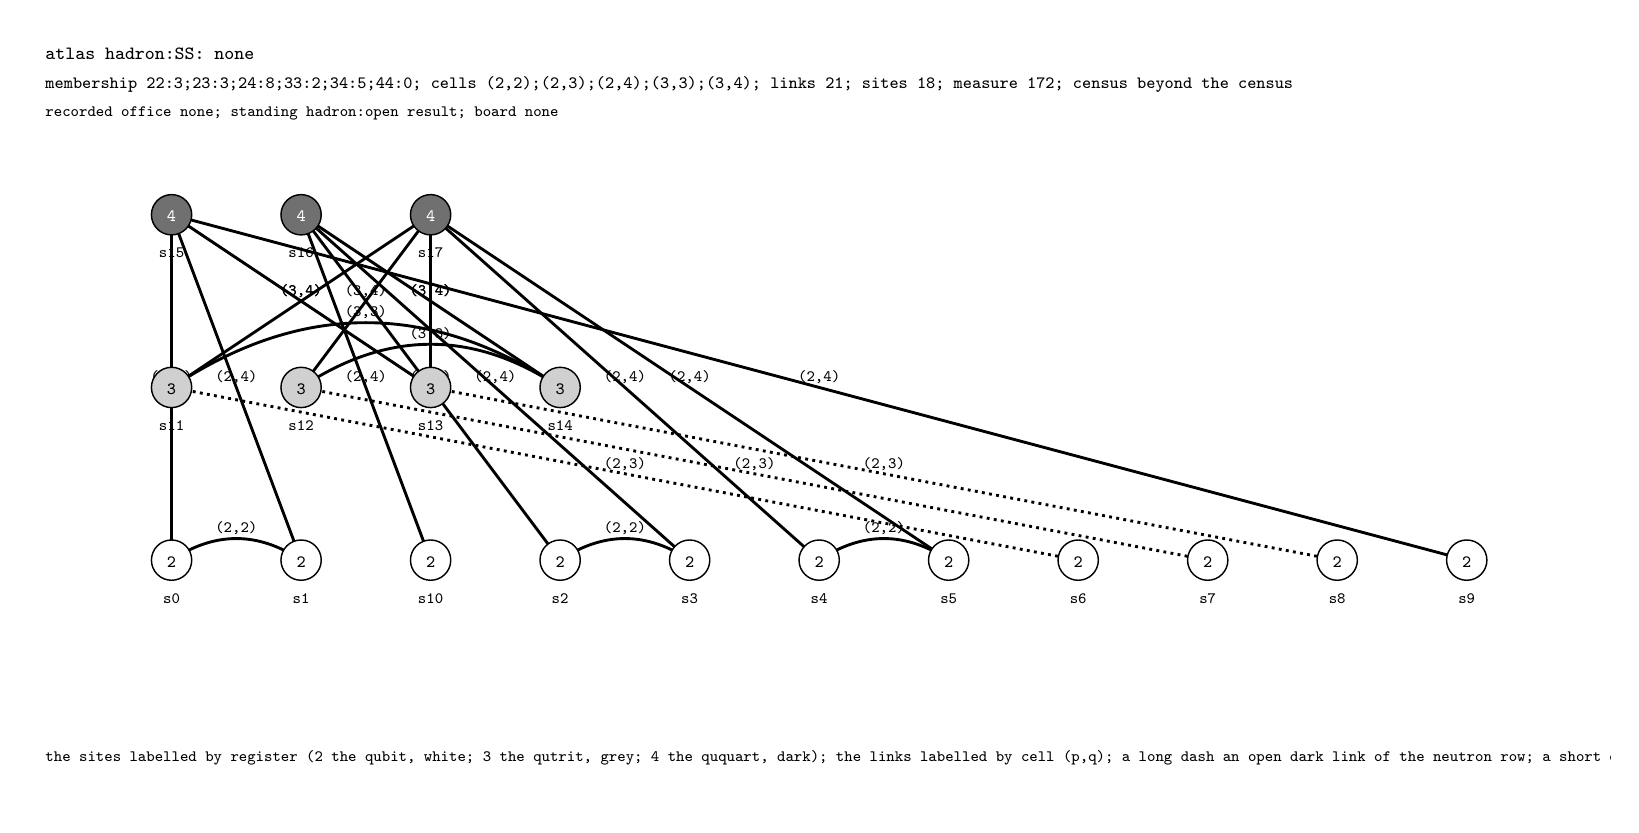
\begin{tikzpicture}[x=0.52pt,y=-0.52pt,baseline]
\clip (0,0) rectangle (1100,540);
\fill[white] (0,0) rectangle (1100,540);
\node[anchor=base west,inner sep=0pt,text=black,font=\fontsize{6.76}{8.112}\selectfont\ttfamily] at (12,22) {atlas hadron:SS: none};
\node[anchor=base west,inner sep=0pt,text=black,font=\fontsize{6.24}{7.488}\selectfont\ttfamily] at (12,42) {membership 22:3;23:3;24:8;33:2;34:5;44:0; cells (2,2);(2,3);(2,4);(3,3);(3,4); links 21; sites 18; measure 172; census beyond the census};
\node[anchor=base west,inner sep=0pt,text=black,font=\fontsize{5.72}{6.864}\selectfont\ttfamily] at (12,62) {recorded office none; standing hadron:open result; board none};
\draw[draw=black,line width=1.04pt] (100,370) -- (100,130);
\node[anchor=base,inner sep=0pt,text=black,font=\fontsize{5.72}{6.864}\selectfont\ttfamily] at (100,246) {(2,4)};
\draw[draw=black,line width=1.04pt] (100,370) .. controls (130,350) and (160,350) .. (190,370);
\node[anchor=base,inner sep=0pt,text=black,font=\fontsize{5.72}{6.864}\selectfont\ttfamily] at (145,351) {(2,2)};
\draw[draw=black,line width=1.04pt] (190,370) -- (100,130);
\node[anchor=base,inner sep=0pt,text=black,font=\fontsize{5.72}{6.864}\selectfont\ttfamily] at (145,246) {(2,4)};
\draw[draw=black,line width=1.04pt] (280,370) -- (190,130);
\node[anchor=base,inner sep=0pt,text=black,font=\fontsize{5.72}{6.864}\selectfont\ttfamily] at (235,246) {(2,4)};
\draw[draw=black,line width=1.04pt] (100,250) .. controls (190,190) and (280,190) .. (370,250);
\node[anchor=base,inner sep=0pt,text=black,font=\fontsize{5.72}{6.864}\selectfont\ttfamily] at (235,201) {(3,3)};
\draw[draw=black,line width=1.04pt] (100,250) -- (280,130);
\node[anchor=base,inner sep=0pt,text=black,font=\fontsize{5.72}{6.864}\selectfont\ttfamily] at (190,186) {(3,4)};
\draw[draw=black,line width=1.04pt,dash pattern=on 1.04pt off 1.56pt] (100,250) -- (730,370);
\node[anchor=base,inner sep=0pt,text=black,font=\fontsize{5.72}{6.864}\selectfont\ttfamily] at (415,306) {(2,3)};
\draw[draw=black,line width=1.04pt] (190,250) .. controls (250,210) and (310,210) .. (370,250);
\node[anchor=base,inner sep=0pt,text=black,font=\fontsize{5.72}{6.864}\selectfont\ttfamily] at (280,216) {(3,3)};
\draw[draw=black,line width=1.04pt] (190,250) -- (280,130);
\node[anchor=base,inner sep=0pt,text=black,font=\fontsize{5.72}{6.864}\selectfont\ttfamily] at (235,186) {(3,4)};
\draw[draw=black,line width=1.04pt,dash pattern=on 1.04pt off 1.56pt] (190,250) -- (820,370);
\node[anchor=base,inner sep=0pt,text=black,font=\fontsize{5.72}{6.864}\selectfont\ttfamily] at (505,306) {(2,3)};
\draw[draw=black,line width=1.04pt] (280,250) -- (100,130);
\node[anchor=base,inner sep=0pt,text=black,font=\fontsize{5.72}{6.864}\selectfont\ttfamily] at (190,186) {(3,4)};
\draw[draw=black,line width=1.04pt] (280,250) -- (280,130);
\node[anchor=base,inner sep=0pt,text=black,font=\fontsize{5.72}{6.864}\selectfont\ttfamily] at (280,186) {(3,4)};
\draw[draw=black,line width=1.04pt,dash pattern=on 1.04pt off 1.56pt] (280,250) -- (910,370);
\node[anchor=base,inner sep=0pt,text=black,font=\fontsize{5.72}{6.864}\selectfont\ttfamily] at (595,306) {(2,3)};
\draw[draw=black,line width=1.04pt] (370,250) -- (190,130);
\node[anchor=base,inner sep=0pt,text=black,font=\fontsize{5.72}{6.864}\selectfont\ttfamily] at (280,186) {(3,4)};
\draw[draw=black,line width=1.04pt] (100,130) -- (1000,370);
\node[anchor=base,inner sep=0pt,text=black,font=\fontsize{5.72}{6.864}\selectfont\ttfamily] at (550,246) {(2,4)};
\draw[draw=black,line width=1.04pt] (190,130) -- (370,370);
\node[anchor=base,inner sep=0pt,text=black,font=\fontsize{5.72}{6.864}\selectfont\ttfamily] at (280,246) {(2,4)};
\draw[draw=black,line width=1.04pt] (190,130) -- (460,370);
\node[anchor=base,inner sep=0pt,text=black,font=\fontsize{5.72}{6.864}\selectfont\ttfamily] at (325,246) {(2,4)};
\draw[draw=black,line width=1.04pt] (280,130) -- (550,370);
\node[anchor=base,inner sep=0pt,text=black,font=\fontsize{5.72}{6.864}\selectfont\ttfamily] at (415,246) {(2,4)};
\draw[draw=black,line width=1.04pt] (280,130) -- (640,370);
\node[anchor=base,inner sep=0pt,text=black,font=\fontsize{5.72}{6.864}\selectfont\ttfamily] at (460,246) {(2,4)};
\draw[draw=black,line width=1.04pt] (370,370) .. controls (400,350) and (430,350) .. (460,370);
\node[anchor=base,inner sep=0pt,text=black,font=\fontsize{5.72}{6.864}\selectfont\ttfamily] at (415,351) {(2,2)};
\draw[draw=black,line width=1.04pt] (550,370) .. controls (580,350) and (610,350) .. (640,370);
\node[anchor=base,inner sep=0pt,text=black,font=\fontsize{5.72}{6.864}\selectfont\ttfamily] at (595,351) {(2,2)};
\filldraw[fill=white,draw=black,line width=0.52pt] (100,370) circle (14);
\node[anchor=base,inner sep=0pt,text=black,font=\fontsize{6.24}{7.488}\selectfont\ttfamily] at (100,375) {2};
\node[anchor=base,inner sep=0pt,text=black,font=\fontsize{5.72}{6.864}\selectfont\ttfamily] at (100,400) {s0};
\filldraw[fill=white,draw=black,line width=0.52pt] (190,370) circle (14);
\node[anchor=base,inner sep=0pt,text=black,font=\fontsize{6.24}{7.488}\selectfont\ttfamily] at (190,375) {2};
\node[anchor=base,inner sep=0pt,text=black,font=\fontsize{5.72}{6.864}\selectfont\ttfamily] at (190,400) {s1};
\filldraw[fill=white,draw=black,line width=0.52pt] (280,370) circle (14);
\node[anchor=base,inner sep=0pt,text=black,font=\fontsize{6.24}{7.488}\selectfont\ttfamily] at (280,375) {2};
\node[anchor=base,inner sep=0pt,text=black,font=\fontsize{5.72}{6.864}\selectfont\ttfamily] at (280,400) {s10};
\filldraw[fill={rgb,255:red,208;green,208;blue,208},draw=black,line width=0.52pt] (100,250) circle (14);
\node[anchor=base,inner sep=0pt,text=black,font=\fontsize{6.24}{7.488}\selectfont\ttfamily] at (100,255) {3};
\node[anchor=base,inner sep=0pt,text=black,font=\fontsize{5.72}{6.864}\selectfont\ttfamily] at (100,280) {s11};
\filldraw[fill={rgb,255:red,208;green,208;blue,208},draw=black,line width=0.52pt] (190,250) circle (14);
\node[anchor=base,inner sep=0pt,text=black,font=\fontsize{6.24}{7.488}\selectfont\ttfamily] at (190,255) {3};
\node[anchor=base,inner sep=0pt,text=black,font=\fontsize{5.72}{6.864}\selectfont\ttfamily] at (190,280) {s12};
\filldraw[fill={rgb,255:red,208;green,208;blue,208},draw=black,line width=0.52pt] (280,250) circle (14);
\node[anchor=base,inner sep=0pt,text=black,font=\fontsize{6.24}{7.488}\selectfont\ttfamily] at (280,255) {3};
\node[anchor=base,inner sep=0pt,text=black,font=\fontsize{5.72}{6.864}\selectfont\ttfamily] at (280,280) {s13};
\filldraw[fill={rgb,255:red,208;green,208;blue,208},draw=black,line width=0.52pt] (370,250) circle (14);
\node[anchor=base,inner sep=0pt,text=black,font=\fontsize{6.24}{7.488}\selectfont\ttfamily] at (370,255) {3};
\node[anchor=base,inner sep=0pt,text=black,font=\fontsize{5.72}{6.864}\selectfont\ttfamily] at (370,280) {s14};
\filldraw[fill={rgb,255:red,112;green,112;blue,112},draw=black,line width=0.52pt] (100,130) circle (14);
\node[anchor=base,inner sep=0pt,text=white,font=\fontsize{6.24}{7.488}\selectfont\ttfamily] at (100,135) {4};
\node[anchor=base,inner sep=0pt,text=black,font=\fontsize{5.72}{6.864}\selectfont\ttfamily] at (100,160) {s15};
\filldraw[fill={rgb,255:red,112;green,112;blue,112},draw=black,line width=0.52pt] (190,130) circle (14);
\node[anchor=base,inner sep=0pt,text=white,font=\fontsize{6.24}{7.488}\selectfont\ttfamily] at (190,135) {4};
\node[anchor=base,inner sep=0pt,text=black,font=\fontsize{5.72}{6.864}\selectfont\ttfamily] at (190,160) {s16};
\filldraw[fill={rgb,255:red,112;green,112;blue,112},draw=black,line width=0.52pt] (280,130) circle (14);
\node[anchor=base,inner sep=0pt,text=white,font=\fontsize{6.24}{7.488}\selectfont\ttfamily] at (280,135) {4};
\node[anchor=base,inner sep=0pt,text=black,font=\fontsize{5.72}{6.864}\selectfont\ttfamily] at (280,160) {s17};
\filldraw[fill=white,draw=black,line width=0.52pt] (370,370) circle (14);
\node[anchor=base,inner sep=0pt,text=black,font=\fontsize{6.24}{7.488}\selectfont\ttfamily] at (370,375) {2};
\node[anchor=base,inner sep=0pt,text=black,font=\fontsize{5.72}{6.864}\selectfont\ttfamily] at (370,400) {s2};
\filldraw[fill=white,draw=black,line width=0.52pt] (460,370) circle (14);
\node[anchor=base,inner sep=0pt,text=black,font=\fontsize{6.24}{7.488}\selectfont\ttfamily] at (460,375) {2};
\node[anchor=base,inner sep=0pt,text=black,font=\fontsize{5.72}{6.864}\selectfont\ttfamily] at (460,400) {s3};
\filldraw[fill=white,draw=black,line width=0.52pt] (550,370) circle (14);
\node[anchor=base,inner sep=0pt,text=black,font=\fontsize{6.24}{7.488}\selectfont\ttfamily] at (550,375) {2};
\node[anchor=base,inner sep=0pt,text=black,font=\fontsize{5.72}{6.864}\selectfont\ttfamily] at (550,400) {s4};
\filldraw[fill=white,draw=black,line width=0.52pt] (640,370) circle (14);
\node[anchor=base,inner sep=0pt,text=black,font=\fontsize{6.24}{7.488}\selectfont\ttfamily] at (640,375) {2};
\node[anchor=base,inner sep=0pt,text=black,font=\fontsize{5.72}{6.864}\selectfont\ttfamily] at (640,400) {s5};
\filldraw[fill=white,draw=black,line width=0.52pt] (730,370) circle (14);
\node[anchor=base,inner sep=0pt,text=black,font=\fontsize{6.24}{7.488}\selectfont\ttfamily] at (730,375) {2};
\node[anchor=base,inner sep=0pt,text=black,font=\fontsize{5.72}{6.864}\selectfont\ttfamily] at (730,400) {s6};
\filldraw[fill=white,draw=black,line width=0.52pt] (820,370) circle (14);
\node[anchor=base,inner sep=0pt,text=black,font=\fontsize{6.24}{7.488}\selectfont\ttfamily] at (820,375) {2};
\node[anchor=base,inner sep=0pt,text=black,font=\fontsize{5.72}{6.864}\selectfont\ttfamily] at (820,400) {s7};
\filldraw[fill=white,draw=black,line width=0.52pt] (910,370) circle (14);
\node[anchor=base,inner sep=0pt,text=black,font=\fontsize{6.24}{7.488}\selectfont\ttfamily] at (910,375) {2};
\node[anchor=base,inner sep=0pt,text=black,font=\fontsize{5.72}{6.864}\selectfont\ttfamily] at (910,400) {s8};
\filldraw[fill=white,draw=black,line width=0.52pt] (1000,370) circle (14);
\node[anchor=base,inner sep=0pt,text=black,font=\fontsize{6.24}{7.488}\selectfont\ttfamily] at (1000,375) {2};
\node[anchor=base,inner sep=0pt,text=black,font=\fontsize{5.72}{6.864}\selectfont\ttfamily] at (1000,400) {s9};
\node[anchor=base west,inner sep=0pt,text=black,font=\fontsize{5.72}{6.864}\selectfont\ttfamily] at (12,510) {the sites labelled by register (2 the qubit, white; 3 the qutrit, grey; 4 the ququart, dark); the links labelled by cell (p,q); a long dash an open dark link of the neutron row; a short dash a docked link at the rule R1};
\end{tikzpicture}\end{adjustbox}
\caption{\texttt{SS of the hadron row}, hadron row body: 18 sites, 21 links, the measure 172; the links at the cells (2,2), (2,3), (2,4), (3,3), (3,4); the membership 22:3; 23:3; 24:8; 33:2; 34:5; 44:0; 3 docked links at the rule R1 (s6-s11; s7-s12; s8-s13); beyond the census of the six cells. Drawn at the anatomy atlas as its web, the sites labeled by register and the links by cell, from the hadron spectroscopy at the cap sinks.}\label{fig:VII-6-D540002-ss-670447}
\begin{center}\footnotesize\begin{adjustbox}{max width=\linewidth}\begin{tabular}{p{0.26\textwidth}p{0.68\textwidth}}\toprule
recorded office (the slot-count row) & no read of this body at the slot-count row \\
mass register (the mass-register row) & no read of this body at the mass-register row \\
\bottomrule\end{tabular}\end{adjustbox}\end{center}
\end{figure}
\end{chconditional}
\chstanding{conditional theorem}
\chdeps{Definitions 1.1 to 1.6, Theorem 172.1 and Open result 172.2, Theorems 174.1 and 174.2 and Open result 174.3 and Open results 245.1 and 245.2, Theorem 245.3, Open results 245.4 to 245.8 and Theorem 245.9}{Open result 178.1, Open result 179.1, Open result 180.1, Theorems 224.1 to 224.3 and Open result 224.4 and Open result 260.1}
The box takes the two nucleon stars with their free docks and lets the pairing move join them. The webs it can no longer act on are listed, and that list, up to eight stars, is what the compendium calls the hadron spectrum.
\begin{chconditional}[The mixed composition, the meson apparatus and the corollaries]\label{box:VII-6-hadron-spectrum-and-the-mesons:2}
Under their parents, the register of the common support, sixteen at every qutrit-qubit dock and eighty-one at every qutrit-qutrit leg and junction reading, is derived at the fourteen docks and the twelve legs of the six docked quark bodies and the two nucleon stars as one register at each reading, so the mixed composition at the eight bodies is defined at the adopted register in one rule; every meson measurement of the table, eleven at the quark and meson rows, is built from the roster cores as a joined web and joined to its apparatus at the hosts of the construction, the measuring body and the measured object an exact web in every case and a value nowhere; and the hadron and nuclear corollaries at the pairing move stand with six gated entries.
\end{chconditional}
\chstanding{conditional theorems, three}
\chdeps{Definitions 1.1 to 1.6, Theorem 172.1 and Open result 172.2, Theorems 174.1 and 174.2 and Open result 174.3 and Open results 245.1 and 245.2, Theorem 245.3, Open results 245.4 to 245.8 and Theorem 245.9}{Open result 178.1, Open result 179.1, Open result 180.1, Theorems 224.1 to 224.3 and Open result 224.4 and Open result 260.1}
The second box gathers the three theorems beside the spectrum.
\begin{chwall}[The direct sum at the deuteron]\label{box:VII-6-hadron-spectrum-and-the-mesons:3}
The direct two-exchange sum at the deuteron web, the two stars paired at the up leaves at one dark qutrit-qutrit link, meets the deuteron office of the earlier result at neither binding entry, while the meson web direct sum is defined as an exact object at every one of the twenty-one pairings of two qutrit cores admitted at the valence bound.
\end{chwall}
\chstanding{open result, built and not closed}
\chdeps{Definitions 1.1 to 1.6, Theorem 172.1 and Open result 172.2, Theorems 174.1 and 174.2 and Open result 174.3 and Open results 245.1 and 245.2, Theorem 245.3, Open results 245.4 to 245.8 and Theorem 245.9}{Open result 178.1, Open result 179.1, Open result 180.1, Theorems 224.1 to 224.3 and Open result 224.4 and Open result 260.1}
The third box names the one reading that parts.
\begin{chbridge}
What this chapter calls the saturated joined webs the literature calls the nuclei, the chain of two neutron stars a dineutron, the web of two neutrons and two protons the alpha particle, the one-link pairing of two quark cores a meson and the pairing move the nuclear binding. The correspondence is by name; the pairing move does not reach the deuteron as a sink.
\end{chbridge}
\begin{chproof}[census]
The premises are the saturation of chapter 1-5, a theorem, the strong coupling of chapter 7-2 and the nucleon star of chapter 7-3, theorems. The chain from the axiom to this chapter is seven chapters long. The set counted is the set of joined webs the pairing move builds from the two stars at their pairable docks, enumerated at every star count from one to four at the dock level and from five to eight at the star level as labeled arrangements, and the property tested is whether the web is a sink of the pairing move, every dock of every star paired. By kind. At one star no sink, the proton star at two free docks and the neutron star at one. At two stars one sink, the chain of two neutrons. At three stars two, the chain neutron-proton-neutron and the proton cycle. At four stars two, the chain of two protons between two neutrons and the proton cycle, and at every count from five to eight two, the chain of proton stars capped by two neutron stars and the cycle of proton stars,
\begin{equation}
14 = 0 + 1 + 2 + 2 + 2 + 2 + 2 + 2 + 1 ,
\end{equation}
with the two-star double pairing beside at the multiple reading. The smallest case is the chain of two neutrons, 30 sites and 33 links, four of genre (2,2), six of (2,3), twelve of (2,4), seven of (3,3) and four of (3,4), its two docks paired and none free, the register 16 at the dock face and 81 at the port face. The web of two neutrons and two protons has 52 sites and 57 links with its six docks all paired, the unique sink at two and two, and the deuteron, the path of one neutron and one proton, is a sink not, its proton dock free. The saturation of the roster is reached at no count to the bound, a count and no claim beyond it.

The site-level isomorphism kinds of the earlier result equal the star-level words at every composition up to four stars at all sixteen label readings, the catalog re-met at 53 kinds with 9 shared groups. The mesons beside are the one-link pairings of the six docked quark bodies at one dark (3,3) link between their cores, a body with its own copy admitted and a body of another kind admitted not at the first reading. For the second box the register of the common support is derived at the fourteen docks and twelve legs as one register at each reading, the eleven meson measurements are built as joined webs with their apparatus, and the corollaries stand at their six gated entries.

\emph{Check.} The sink test was carried at both multiplicity readings, the sinks within a web beside the sinks of the pairing, with the deuteron and helium-3 checked by name as sinks never and the triton as a sink. The result was reproduced by an independent route, two engines at every capture byte for byte, its five counter-tests at their pinned letters and its controls the same at both routes.
The direct sum at the deuteron meets the deuteron office at neither binding entry, and the six gated entries of the corollary theorem stand gated. The nuclear rows at the joined seeded web are the matter of chapter 9-7.
\chcert{14}
\end{chproof}
\label{chend:VII-6-hadron-spectrum-and-the-mesons}
\section{The heavy-flavor sinks at the hadron rows}\label{mod:VII-6-D539921-w-hfhd}
\begin{chwall}[The heavy-flavor sinks at the hadron rows]\label{box:VII-6-D539921-w-hfhd:1}
This result is conditional on the parents at their grades, the decay board an instrument and the hadron-spectrum, bound-respecting, proton-web and rep-census entries read at their grades, the composition riding the lowest grade in its chain. Under the axiom text, the dock rule and the parent results, every heavy sink carries its office of the form the item words, the cap of the (2,3) genre squared multiplied by nine to the exponent of its dressing, 74183769, 667653921, 74183769 and 8242641 at the charm, strange, bottom and top sinks, and the current-mass entries of the board are of another kind, the quark words docked bodies without a junction leg and the sinks saturated webs with junction legs, their webs and offices parting at four of four; but no heavy sink is placed at a hadron row of the decay board or at a spectrum row by its structure at the reading adopted, the dock count, the arm count at the center-and-hub-removed reading and the hub count equal to no row web at zero of four: the charm sink at two docks, two arms and two hubs, the strange and the top sinks at three, three and three, the bottom sink at two, two and three, against the proton row at three, three and one, the neutron row at three, three and two and the roster webs at three docks per star, the twenty-seven meson and baryon rows of the decay board carrying no sink at that depth; the heavy sinks match the one-link meson pairings of the hadron-spectrum entry beside, the charm sink the charm word paired with itself, at the center-and-hub-removed reading alone, printed beside; the first parting the charm sink.
The first face, each heavy sink placed at a hadron row of the decay board or the spectrum rows by its structure with its office beside the row and the current-mass entries typed as a parting of kind, reads no, the sinks placed zero of four while the kind typing parts at four of four; the second face, a heavy sink placed at no hadron row named, reads yes at the first parting of the item order, the charm sink. Open is the placement of the heavy sinks at the hadron rows: their structures match no row web at the reading adopted, and they match meson pairings at one reading beside alone.
\end{chwall}
\chstanding{an open result}
\chdeps{Definitions 1.1 to 1.6 and Theorems 177.1 and 177.2 and Open result 177.3}{no theorem beyond it at this release}
The four heavy sinks, the first saturated sinks reached at each heavy flavor, carry offices of one form, the hadron cap squared multiplied by a power of nine fixed by the dressing. The question is whether each sits at a hadron row, of the decay board or of the spectrum, when both are described by the same triple, the number of docks, the number of arms once the center and the hubs are removed, and the number of hubs. None does: the proton row has one hub and three docks, the neutron row two hubs and three docks, the spectrum webs three docks per star, while the charm sink has two of each, and the twenty-seven meson and baryon rows of the board carry no sink web at all. The quark words of the current-mass entries are a different kind of object, docked bodies with no junction leg, so the heavy sinks are neither the hadron rows nor the quarks, and only at one reading beside do they match meson pairings.
\begin{chbridge}
The heavy quarks of the Standard Model, charm, strange, bottom and top, are confined into mesons and baryons whose masses are set by the strong interaction and the quark masses together, the quark masses themselves scheme-dependent parameters rather than observable rest masses \cite{Gasser1982,Peskin1995}. The correspondence is by name.
\end{chbridge}
\begin{chproof}[exhaustive census with its exact part]
The premises of this derivation are the axiom and the six definitions of chapter~\ref{mod:FRAMEWORK}, the hadron spectrum and the mesons of the present chapter, a theorem, the quark content and flavor of chapter~\ref{mod:VII-7-quark-content-and-flavour}, a theorem, the proton as a seeded sink of chapter~\ref{mod:VII-4-proton-as-a-seeded-sink}, a theorem, the body-alone office rule of chapter~\ref{mod:VIII-2-body-alone-office-rule}, a theorem, and the decay board of chapter~\ref{mod:IX-1-decay-as-the-forward-edge-of-a-non-sink-the-move-graph-of-the-hub-step}, an instrument. The chain of premises runs back to the axiom through those chapters, and the longest such chain in this compendium is twelve chapters long.
\textit{The exact part.} The office of each heavy sink is the cap of the (2,3) genre, 319 at the cap census, squared and multiplied by nine to the exponent of its dressing,
\begin{equation} \adjustbox{max width=\dimexpr\linewidth-3em\relax}{$\displaystyle \Omega_{c} = 319^{2}\cdot 9^{3} = 74183769, \quad \Omega_{s} = 319^{2}\cdot 9^{4} = 667653921, \quad \Omega_{b} = 319^{2}\cdot 9^{3} = 74183769, \quad \Omega_{t} = 319^{2}\cdot 9^{2} = 8242641,$} \end{equation}
each a cell of the quark-offices entry re-met by locator at four of four, exact of the form at four of four. The structure of a web is its dock count by the dock rule, the pendant end the smaller end of the genre, its arm count at the center-and-hub-removed reading and its hub count by the hub rule, and a sink is placed at a row when its triple equals the triple of the row web. The figure draws the triple of the charm sink beside that of the proton row.
\textit{The census.} By exhaustive enumeration of the four heavy sinks against the forty-three hadron rows, the twenty-nine rows of the decay board, the proton row at the sink of the bound-respecting entry with eight sites, nine links and the triple three, three, one, the neutron row at the proton-web seed with thirteen sites, sixteen links and the triple three, three, two, and the twenty-seven meson and baryon rows at no sink at that depth, their structure undefined, together with the fourteen roster webs of the hadron spectrum re-met at their sites, links and genre census at fourteen of fourteen, from the triple six, four, two at two stars to twenty-four, seventeen, ten at eight: the property tested is equality of the triples; the counts are placed at zero of four at the reading adopted, the charm sink at two, two, two, the strange and the top at three, three, three and the bottom at two, two, three equal to no row; printed beside, at the whole triple the charm sink equals the meson pairing of the charm word with itself and the strange and top sinks their pairings, at the center-and-hub-removed reading alone. The kind typing: each sink is a saturated web carrying junction legs, three at the charm, two at the strange, three at the bottom and three at the top, and the docked quark word of the flavor carries none, their webs parting at four of four, fifteen sites against six, eighteen against ten, sixteen against thirteen and seventeen against nine, and their offices parting at four of four, 74183769 against 101761, 667653921 against 8242641, 74183769 against 8242641 and 8242641 against 101761. The smallest case is the charm sink against the proton row, two docks against three.
\textit{The check.} The counter-tests alter the construction singly and read what moves. Reading the charm sink at the library copy moves its triple, forty-seven cells. Striking the first hub of the charm sink moves its hub count, twenty-eight cells. Reading the placement at the hub axis alone places the charm sink at the neutron row, thirty-four cells. Striking the text unmeets the gate. Each alteration moves the cells it names, four of four. The result was reproduced by an independent route, two engines built apart, a map-and-set route against the second route, equal at every cell, with the fourteen controls the same and the office runs equal at ten of ten.
\chcert{43}
\begin{figure}[h]\centering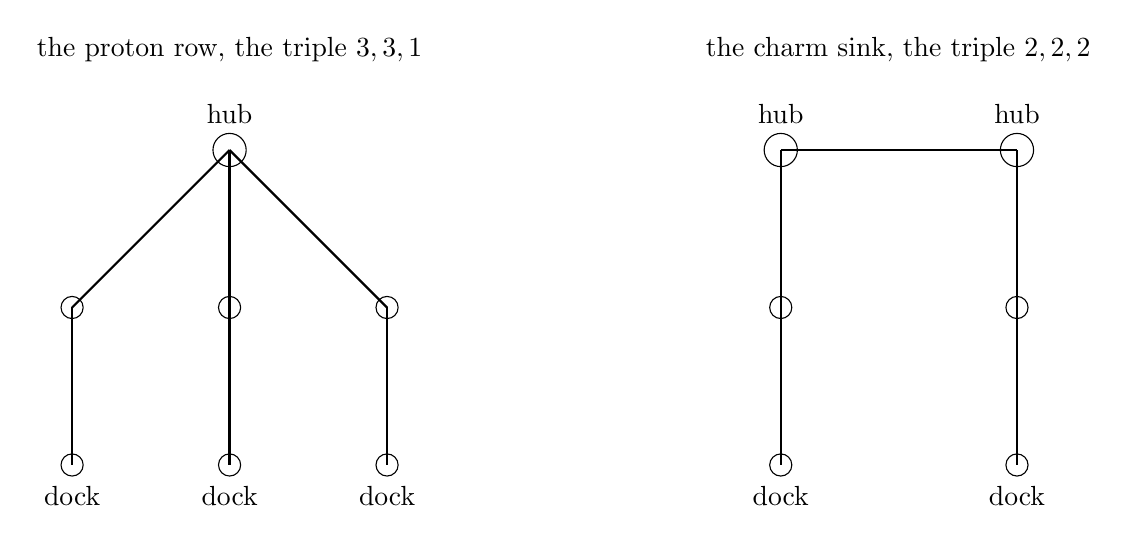
\begin{tikzpicture}[scale=1]
\filldraw[fill=white] (0,0) circle (6pt) node[above=6pt] {hub};
\foreach \a in {-2,0,2} {\filldraw[fill=white] (\a,-2) circle (4pt); \draw[thick] (0,0) -- (\a,-2); \filldraw[fill=white] (\a,-4) circle (4pt) node[below=4pt] {dock}; \draw[thick] (\a,-2) -- (\a,-4);}
\node at (0,1) [above] {the proton row, the triple $3, 3, 1$};
\filldraw[fill=white] (7,0) circle (6pt) node[above=6pt] {hub}; \filldraw[fill=white] (10,0) circle (6pt) node[above=6pt] {hub};
\draw[thick] (7,0) -- (10,0);
\foreach \a in {7,10} {\filldraw[fill=white] (\a,-2) circle (4pt); \draw[thick] (\a,0) -- (\a,-2); \filldraw[fill=white] (\a,-4) circle (4pt) node[below=4pt] {dock}; \draw[thick] (\a,-2) -- (\a,-4);}
\node at (8,1) [above, xshift=14pt] {the charm sink, the triple $2, 2, 2$};
\end{tikzpicture}\caption{The structure triples compared: the proton row with three docks, three arms and one hub, and the charm sink with two docks, two arms and two hubs, drawn as schematics of their counts.}\end{figure}
\end{chproof}
\section{Hadron spectroscopy at the cap sinks}\label{mod:VII-6-D540002-w-hadx}
\begin{chwall}[Hadron spectroscopy at the cap sinks]\label{box:VII-6-D540002-w-hadx:1}
This result is conditional on the wave budget of its source and on the parent results at their grades, the open results among them read at their grades. The first sink with no first power is named with its cells: the gluon-only sink 94 of the proton-web saturation at wave two, the docks zero at the census typing, every (2,3) link of it pendant at its qutrit end, fourteen sites, eighteen links, the measure 143, the entry dock none and the first power no hub at both engines under the dock rule. The open result face: at the dock rule and the typing adopted every excited sink with a pendant-qubit dock carries a first power 319 multiplied by a power of three, 234 of 276, the ladders at six and three distinct first powers with no read at the swapped cap, and every excited sink without one carries none, 42 of 276, the four gluon-only sinks of the three-quark saturation and the thirty-eight dock-free cap sinks of the two-quark saturation; both faces printed at every class.
The first face, every excited sink of the two saturations within the budget a cell with a first power by the segment theorem, reads no at 234 of 276; the second face, the first sink with no first power named with its cells, reads yes at the sink 94. Open is the first power at the dock-free sinks: a read enters a sink at a dock alone, the pendant qubit of a (2,3) link, and a sink with no such link is entered nowhere.
\end{chwall}
\chstanding{an open result}
\chdeps{Definitions 1.1 to 1.6 and Theorems 177.1 and 177.2 and Open result 177.3}{no theorem beyond it at this release}
The excited states of the hadron spectrum are read here as the saturated sinks beyond the ground state of two saturations, the three-quark saturation seeded at the proton web, 181 sinks within the wave budget of the entry, and the two-quark saturation at the pion web, 96 cap sinks. The first power of a sink by the segment theorem is read by entering at its first dock, the pendant qubit of a (2,3) link, capping the entered link at the cap of the genre, 319, stopping at the first hub and dressing the entry segment by three for every in-leg left unpassed. Every sink that has a dock gets a first power of the form 319 multiplied by a power of three, and the first powers fall on ladders, six distinct values in the three-quark saturation and three in the two-quark, with exact ratios to the ground states. But a sink whose (2,3) links are all pendant at the qutrit end has no dock, no entry and no first power, and the open result names the first such sink, a gluon-only sink of the proton-web saturation.
\begin{chbridge}
Hadron spectroscopy lists the excited states of mesons and baryons on Regge trajectories, their masses rising with the spin and the radial excitation, and the glueballs, bound states of gluons alone, are predicted by the theory and not yet identified \cite{Chew1962,Mathieu2009}. The correspondence is by name.
\end{chbridge}
\begin{chproof}[exhaustive census with its exact part]
The premises of this derivation are the axiom and the six definitions of chapter~\ref{mod:FRAMEWORK}, the hadron spectrum and the mesons of the present chapter, a theorem, the proton as a seeded sink of chapter~\ref{mod:VII-4-proton-as-a-seeded-sink}, a theorem, the quark content and flavor of chapter~\ref{mod:VII-7-quark-content-and-flavour}, a theorem, and the first power as the sum over the segments of the read of chapter~\ref{mod:VIII-1-mass-unit-and-the-first-power}, a theorem. The chain of premises runs back to the axiom through those chapters, and the longest such chain in this compendium is twelve chapters long.
\textit{The exact part.} The first power of a sink by the segment theorem is the cap of the entered genre, 319 at the (2,3) genre, multiplied by three to the number of in-legs the read leaves unpassed at the first hub,
\begin{equation} S_{1} = 319\cdot 3^{u}, \qquad \frac{S_{1}}{S_{1}(\text{ground})} \in \Big\{\tfrac{1}{9},\ \tfrac{1}{3},\ 1,\ 3,\ 9,\ 243\Big\} \ \text{over } 2871 \ \text{and} \ \{1,\ 3,\ 9\} \ \text{over } 319, \end{equation}
the ground state of the three-quark saturation at $2871 = 319\cdot 9$ and of the two-quark saturation at $319$, every ratio an exact rational reduced at two routes, 234 of 234, and the ratios over the electron unit 67 alike. The figure draws a (2,3) link pendant at its qubit end, a dock, beside one pendant at its qutrit end, which is no dock.
\textit{The census.} By exhaustive enumeration of the 276 excited sinks, the 180 sinks beyond the ground state of the three-quark saturation within the wave budget, waves zero to two, and the 96 cap sinks of the two-quark saturation beyond its first, each listed at its anatomy equal to its sites, links and measure by locator, 279 of 279 reads the same: the property tested at each sink is whether a read enters it at a dock, a (2,3) link pendant at its qubit end, so that the segment theorem gives a first power; the counts by class are a first power defined at 234 of 276, 176 of 180 three-quark and 58 of 96 two-quark, and no hub at 42 of 276, every one typed dock-free by locator, the four gluon-only sinks 94, 111, 136 and 139 of the three-quark saturation and the 38 dock-free cap sinks of the pion web. The first parting element is the sink 94 at wave two, dark by the dock count and by the form, with fourteen sites, eighteen links, the measure 143, two hubs and the genre census (2,2) two, (2,3) four, (2,4) six, (3,3) three and (3,4) three, every (2,3) link pendant at its qutrit end, so the entry dock is none, the first power no hub and the office undefined. The smallest case worked is the ground state itself, the seed web of ten sites and twelve links at the measure 101, read at two roots equal.
\textit{The check.} The counter-tests alter the construction singly and read what moves. The four parent strikes at every root, the arm struck from the star sum, the flavor selection flipped, the charm sink read at the library copy and the text struck, move their named cells at twelve of twelve pieces. Striking the dock dimension to the qutrit enters sixteen sinks at the swapped cap 475 and moves 342 of 345 cells. Striking the typing to uncapped moves the ground office from 2871 to 747 and 261 of 551 cells. Each alteration moves the cells it names, fourteen of fourteen. The result was reproduced by an independent route, two engines built apart, the python route against the perl route, equal at every cell, with the twenty-five controls the same and the parent engines on their own image equal at twenty-two of twenty-two pairs.
\chcert{276}
\begin{figure}[h]\centering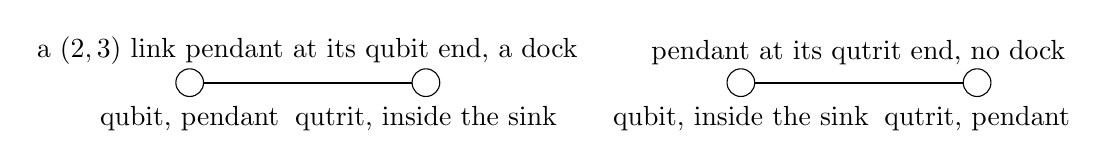
\begin{tikzpicture}[scale=1]
\draw[thick] (0,0) -- (3,0);
\filldraw[fill=white] (0,0) circle (5pt) node[below=5pt] {qubit, pendant};
\filldraw[fill=white] (3,0) circle (5pt) node[below=5pt] {qutrit, inside the sink};
\node at (1,0) [above=3pt, xshift=14pt] {a $(2,3)$ link pendant at its qubit end, a dock};
\draw[thick] (7,0) -- (10,0);
\filldraw[fill=white] (7,0) circle (5pt) node[below=5pt] {qubit, inside the sink};
\filldraw[fill=white] (10,0) circle (5pt) node[below=5pt] {qutrit, pendant};
\node at (8,0) [above=3pt, xshift=14pt] {pendant at its qutrit end, no dock};
\end{tikzpicture}\caption{The dock rule: a read enters a sink at the pendant qubit of a (2,3) link alone; the gluon-only sink 94 has four (2,3) links, every one pendant at its qutrit end, and so no entry.}\end{figure}
\end{chproof}
\section{The hadron offices from membership}\label{mod:VII-6-D543708-w-hdom}
\begin{chwall}[The hadron offices from membership]\label{box:VII-6-D543708-w-hdom:1}
The office formula at the junction register parts from the offices of the nucleon and the hadron sinks, the first parting the proton sink: the formula with its first-power bracket at the junction register of the share face at the dressing is met at zero of thirteen reads, the first parting the proton sink, its first power 729 against 2871, located at a count, the share-face register 81 against the cap 319 of the (2,3) genre, the Born count of the count law, at the dressing exponent two; the capped reads are met at the cap register with the closure zero, seven of thirteen, and the hub-count-two sinks at the dock-struck bracket, four of thirteen; the first face unmet at the reading adopted, the second face met with the first parting named with both cells; every cell an exact element of the field of root two and root three compared with nothing.
The first face, every established office of the nucleon and the hadron sinks met by the formula at the junction register, reads no, the formula met at zero of thirteen; the second face, the first parting named and located at a count, reads yes at the proton sink. Open is the first power of a hadron read as a formula in its membership counts: at the junction register of the share face the bracket gives 81 where the capped read of the nucleon gives 319, and the formula meets the capped reads only at the cap register and the hub-count-two sinks only at the dock-struck bracket.
\end{chwall}
\chstanding{an open result}
\chdeps{Definitions 1.1 to 1.6 and Theorems 177.1 and 177.2 and Open result 177.3}{no theorem beyond it at this release}
The office-as-a-formula entry of the mass chapter writes the office of a body in the six membership counts of its links by genre, with a first-power bracket and a closure at the counts, and this entry asks whether that formula, evaluated with the bracket at the junction register of the share face, re-meets the offices of the nucleon and of the hadron sinks. The junction register of the proton star is 81, the (3,3) register of its three junction legs at a share of one third each, and multiplied by the dressing at the exponent two it gives a first power of 729, while the office of the proton sink has the first power 2871, the cap 319 of the (2,3) genre multiplied by nine. The two part at one count, the share-face register against the cap, and the same parting stands at every nucleon read, while the capped reads are met if the cap register is used and the hub-count-two sinks if the dock-struck bracket is; the three hadron open results of the chapter are re-read as instances of the formula at a count.
\begin{chbridge}
The mass of a hadron is in the standard account the sum of its constituent masses and its binding, with the proton mass set almost entirely by the strong interaction among three light quarks joined at a color-singlet vertex \cite{Gasser1982,Peskin1995}. The correspondence is by name.
\end{chbridge}
\begin{chproof}[exact-cell derivation with its census]
The premises of this derivation are the axiom and the six definitions of chapter~\ref{mod:FRAMEWORK}, the hadron spectrum and the mesons of the present chapter, a theorem, the proton as a seeded sink of chapter~\ref{mod:VII-4-proton-as-a-seeded-sink}, a theorem, the nucleon structure and the form factor of chapter~\ref{mod:VII-3-nucleon-structure-and-the-form-factor}, a theorem, the body-alone office rule of chapter~\ref{mod:VIII-2-body-alone-office-rule}, a theorem, and the office as a formula in the membership counts of chapter~\ref{mod:VIII-1-mass-unit-and-the-first-power}, an open result. The chain of premises runs back to the axiom through those chapters, and the longest such chain in this compendium is twelve chapters long.
\textit{The exact part.} The proton sink carries the membership vector $(0, 3, 0, 3, 3, 0)$ over the genres (2,2), (2,3), (2,4), (3,3), (3,4) and (4,4), the struck vector $(0, 3, 0, 0, 0, 0)$, the dressing exponent two and the share-face register 81 at its junction site, a qutrit of degree three whose three (3,3) legs carry the share one third each, summing to one. The formula at the junction register gives the first power
\begin{equation} S_{1}^{\mathrm{formula}} = 81\cdot 3^{2} = 729 \qquad \text{against} \qquad S_{1}^{\mathrm{office}} = 319\cdot 9 = 2871 , \end{equation}
so the parting is located at one count, the share-face register 81 against the cap 319 at the dressing exponent two, and the formula cell, an element of the field with a sixteen-digit rational coordinate and a root-three coordinate printed at the table of the entry, parts from the office 8242641 of the proton sink. The figure draws the junction site of the proton star.
\textit{The census.} By exhaustive enumeration of the seventeen reads, the proton sink, the neutron through the deuteron and the strike-rule neutron, the proton star, the four heavy sinks, the four gluon-only sinks and the five hub-count-two sinks, each with its junction sites, its junction registers at the share face, the dock-struck reading and the hub-product reading, and its membership vector, re-met against the junction-star and census entries at every read: the property tested at each of the thirteen reads carrying an office is whether the formula at the junction register of the share face at the dressing, with the closure at the counts, equals the office; the counts are met at zero of thirteen at the reading adopted, the capped reads of the body-alone and heavy-flavor entries met at the cap register with the closure zero at seven of thirteen, and the hub-count-two sinks met at the dock-struck bracket with the closure at the counts at four of thirteen; the gluon-only sinks carry no office and are compared with nothing; the three hadron open results of the chapter are instances of the formula at a count at three of three, the gluon-only sink at the dock count, the heavy sinks at the dock and hub counts and the hub-count-two sink at the membership vectors. The smallest case is the proton sink worked above.
\textit{The check.} The counter-tests alter the construction singly and read what moves. Striking the first (3,3) leg at the first junction center moves the registers at every read with a junction site. Adding a (3,3) end to every membership vector moves the formula cells. Dropping the closure moves every read with a nonzero closure. Reading a word of the library with no junction, the docked top word, holds at the cells with its formula cell printed and compared with nothing. Striking the gate exits at both engines. Each alteration moves the cells it names, five of five. The result was reproduced by an independent route, two engines built apart, the explicit record-space route against the second route, equal at every cell, with the fifteen controls the same.
\chcert{17}
\begin{figure}[h]\centering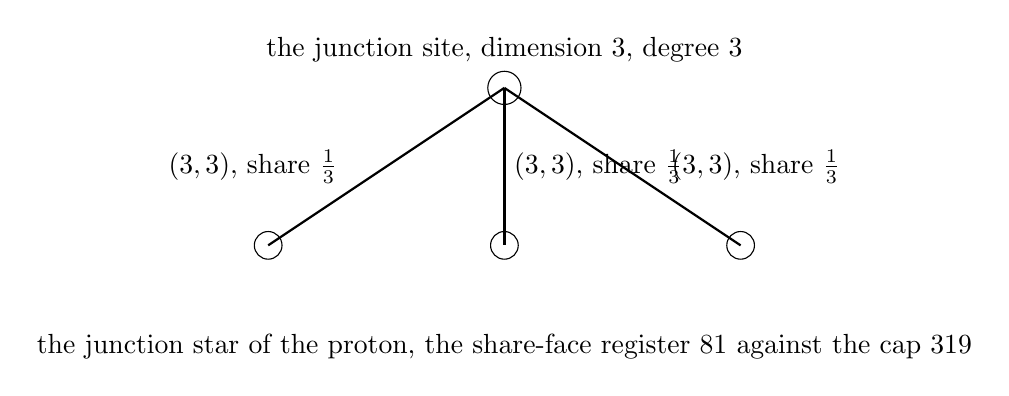
\begin{tikzpicture}[scale=1]
\filldraw[fill=white] (0,0) circle (6pt) node[above=6pt] {the junction site, dimension 3, degree 3};
\foreach \a in {-3,0,3} {\filldraw[fill=white] (\a,-2) circle (5pt); \draw[thick] (0,0) -- (\a,-2);}
\node at (-2,-1) [left] {$(3,3)$, share $\tfrac{1}{3}$}; \node at (0,-1) [right] {$(3,3)$, share $\tfrac{1}{3}$}; \node at (2,-1) [right] {$(3,3)$, share $\tfrac{1}{3}$};
\node at (0,-3) [below] {the junction star of the proton, the share-face register $81$ against the cap $319$};
\end{tikzpicture}\caption{The junction site of the proton star with its three (3,3) legs at a share of one third each; the formula at its register gives the first power 729 where the capped read gives 2871.}\end{figure}
\end{chproof}
\par\medskip\noindent{\itshape The spectrum read, the next chapter reads what the hadrons are made of.}\label{narr:close:7-6}\par
\section{Quark content and flavour}\label{mod:VII-7-quark-content-and-flavour}
\chdesig{9-7}{7-7}{VII-7-quark-content-and-flavour}{VII-7-D539669-udao-t1}
\label{narr:open:7-7}Theorem~181.1 reads the quark register at the second-order junction read, Theorem~181.2 flavor as the rung name with the quark ladder, Open result~181.3 the five readings beside, Theorem~181.4 the quark ladder at the saturated sinks, and Theorem~181.5, a theorem, the quark offices as the star arm reads.
\begin{chconditional}[The quark register at the second-order junction read]\label{box:VII-7-quark-content-and-flavour:1}
Under its parents, the read engine run through every junction star at order two reads every leg with the entering link at the cut register, so the junction entry of a second read link is one exact object, eight at the cut reading, equal to the cut-reading bound at every one of the six quark bodies, and the share is the colour third, one third per leg; the junction tensor at the two-read junction of the down body equals the bounded tensor at the count ratio one third.
\end{chconditional}
\chstanding{conditional theorem}
\chdeps{Definitions 1.1 to 1.6, Theorem 171.1 and Open result 171.2, Theorems 174.1 and 174.2 and Open result 174.3 and Open results 241.1 and 241.2, Theorems 241.3 and 241.4 and Open results 241.5 to 241.7}{Theorem 27.1, Theorem 181.4, Theorem 181.5, Chapter 9-7 and Chapter 9-7}
The box reads each quark body as a star centered on its junction qutrit and finds that every leg of the star takes exactly one third of the read, the color third, and that the entry of a leg read at second order is one exact number equal to the bound.
\begin{chconditional}[Flavor as the rung name and the quark ladder]\label{box:VII-7-quark-content-and-flavour:2}
Under their parents, flavour is the rung name read at the corner: the three corner frames of the charged-lepton dark triangle at one, two and three hub legs equal the three residues of the adopted naming at every corner, the residue of the depth momentum read there; and the hub step applied at the up and down bodies with the junction legs kept at one and two steps gives the quark ladder, its hub counts and generation labels compared with the roster ladders.
\end{chconditional}
\chstanding{conditional theorems, two}
\chdeps{Definitions 1.1 to 1.6, Theorem 171.1 and Open result 171.2, Theorems 174.1 and 174.2 and Open result 174.3 and Open results 241.1 and 241.2, Theorems 241.3 and 241.4 and Open results 241.5 to 241.7}{Theorem 27.1, Theorem 181.4, Theorem 181.5, Chapter 9-7 and Chapter 9-7}
The second box gathers the two theorems on flavor, what names a generation, and how the heavier quarks are reached from the lighter by the hub step.
\begin{chwall}[The five readings beside]\label{box:VII-7-quark-content-and-flavour:3}
The slot-star register of the junction read and the vertex leg register are one object at a junction star whose other legs are unread and two objects at the star carrying a second read link, the whole 36 against the cut 24; the entry of a leg bounded by the share rule is one third of the pair-ket unit, 12 at the whole reading and 8 at the cut reading, parting at the two-read junction of the down quark; the six quark-body types are typed from the roster alone at six distinct arm signatures, but the typed count is not a first-order register count; the hub-leg cut is not the selection rule for quark flavour either, the twenty hub-leg cuts that change a count each losing one quark and gaining a quark pair; and the quark content as the set of the star reads at one arm parts at the lepton weight against the weight one with the colour.
\end{chwall}
\chstanding{open results, five, built and not closed}
\chdeps{Definitions 1.1 to 1.6, Theorem 171.1 and Open result 171.2, Theorems 174.1 and 174.2 and Open result 174.3 and Open results 241.1 and 241.2, Theorems 241.3 and 241.4 and Open results 241.5 to 241.7}{Theorem 27.1, Theorem 181.4, Theorem 181.5, Chapter 9-7 and Chapter 9-7}
The third box names the readings tried and parted.
\begin{chbridge}
What this chapter calls the color third the literature calls the color charge of a quark, the junction read the color-singlet projection and the rung name the generation number, the nearest objects. The correspondence is by name, and no quark mass is displayed here.
\end{chbridge}
\begin{chproof}[finite computation]
The premises are the moves of chapter 1-4, a definition, confinement of chapter 7-1 and the nucleon star of chapter 7-3, theorems. The chain from the axiom to this chapter is seven chapters long. The procedure. The input is the six quark bodies of the catalog with the first-order dock at each and the junction site of dimension 3, three junction stars (the down, the strange and the bottom) and three chain bodies (the up, the charm and the top), each leg typed read or unread by its genre. The enumeration runs the read engine through every star at order two at both polarities, the junction-center polarity and the larger-dimension polarity, the count law at every leg with the traceless dimensions at the far end and the center. The test compares the junction entry of a second read link with the bound. The aggregation forms the per-leg share. The smallest instance is one leg of a junction star, the share is the color third, the pair ket at dimension three flat at
\begin{equation}
\frac{1}{3}, \frac{1}{3}, \frac{1}{3}, \qquad \frac{1}{3} + \frac{1}{3} + \frac{1}{3} = 1 ,
\end{equation}
multiplied by the leg readout, at every (2,3) leg
\begin{equation}
\frac{79}{62208} + \frac{1}{1296}\sqrt{2} + \frac{7}{10368}\sqrt{3} + \frac{1}{20736}\sqrt{6} ,
\end{equation}
an exact element of the field of root two and root three, at 8 of 8 stars over 21 legs at both polarities. The junction entry at the cut reading is 8, equal to the bound at 6 of 6 bodies, and the up body at the first-order office $36/4489$ at the dock unit.

From the three corner frames of the charged-lepton dark triangle at one, two and three hub legs, by the residue of the depth momentum modulo three, we obtain the three residues of the adopted naming at every corner, flavor as the rung name. From the up and down bodies, by the hub step with the junction legs kept at one and two steps, we obtain the quark ladder with its hub counts and generation labels compared with the roster ladders. The five readings beside part at their named steps.

\emph{Check.} The first cut of this entry stood beyond the never-input gate and was set aside with its content confirmed at every part. The re-fire re-derived every cell at both engines. The result was reproduced by an independent route, two engines at every capture byte for byte, its five counter-tests at their pinned letters and its twelve controls the same at both routes.
The register at the junction read at its deciding reading, the bounded entry at the two-read junction, the selection rule for flavor and the content at an unequal far end stay open.
\chcert{21}
\end{chproof}
\label{chend:VII-7-quark-content-and-flavour}
\subsection{The quark ladder at the saturated sinks}\label{mod:VII-7-D536267-qlsk-t1}
\begin{chconditional}[The quark ladder at the saturated sinks]\label{box:VII-7-D536267-qlsk-t1:1}
Under its parents, the open results among them, the four heavy-flavour first powers, the strange, the charm, the bottom and the top, are outputs of the hub lowering at the saturated sinks, each a rank multiplied by a dressing: the first reached charm 147 by 81, strange 172 by 243, top 165 by 108 and bottom 171 by 324, with 19, 82, 51 and 87 distinct reached values per flavour, and the top-to-W ratio 891 at the first reached top a cell beside.
\end{chconditional}
\chstanding{conditional theorem}
\chdeps{Definitions 1.1 to 1.6 and Theorems 181.1 and 181.2 and Open result 181.3}{no theorem beyond it at this release}
The box reaches the four heavy quarks from the stable webs of the saturation by one move, the lowering of a hub, and reads the first power of each web reached as the product of a rank and a dressing. Every one of the four flavors is reached.
\begin{chbridge}
What this chapter calls the hub lowering at a sink the literature calls a flavor transition, the first power of the reached web the mass of the heavy quark and the top-to-W ratio the ratio of the top and W masses. The correspondence is by name, and the quark rows are compared with experiment at the comparison table alone.
\end{chbridge}
\begin{chproof}[census]
The premises are the quark content chapter above and the framework. The chain from the axiom to this result is eight chapters long. The set counted is the set of quark-form sinks, 16788 webs, the fourteen roster webs, the 16773 proton sinks of the saturation and the bound-respecting seed, every one re-cut whole from its source and re-met at its census row at 16788 of 16788. The property tested is whether the sink admits a step of the hub lowering, at a qutrit core with spare or at a hub carrying an odd leg, and the flavor and first power of the web the step reaches. By kind. 1005 of the 16788 sinks admit no step, every core saturated and every hub without an odd leg, the first the proton web of the saturation itself. The lowering at the rest gives 155649 lowered webs at the five step readings, 154111 within the valence bound at the touched site, and the steps of the construction 41455, each lowered web built as sites and links with its first power a rank multiplied by a dressing, an exact integer. The four flavors are reached by the step of the construction at the reading by isomorphism, the charm at 29 lowered webs reaching 28 distinct sinks, the strange at 166 reaching 159, the top at 120 reaching 117 and the bottom at 174 reaching 170, the first reached of each
\begin{equation}
147 \cdot 81 = 11907, \qquad 172 \cdot 243 = 41796, \qquad 165 \cdot 108 = 17820, \qquad 171 \cdot 324 = 55404 ,
\end{equation}
with 19, 82, 51 and 87 distinct reached first powers per flavor. The smallest case is the W first power at the hub of the step, the rank of its leaf pair,
\begin{equation}
20 = 8 + 8 + 4 ,
\end{equation}
the two (2,4) legs and the (2,2) pair, equal to the W form at the leaf pair of the W-read entry at 24 of 24 generation edges, and the top-to-W ratio at the first reached top $17820/20 = 891$.

The top-to-W ratio at every top lowered web is a reduced fraction, the first $2016/5$ at the roster web, the least $1431/5$, the greatest $6757095168/5$, 698 distinct, the cataloged top beside at $246/5$. Compared with nothing.

\emph{Check.} The sinks admitting no step, 1005, are named at their first. The lowered webs beyond the valence bound at the touched site, 1538, are excluded and counted. The result was reproduced by an independent route, two engines at every capture byte for byte, its counter-tests at their pinned letters and its controls the same at both routes.
The sinks admitting no step stay open, and the comparison of the flavor figures stands at the comparison table.
\chcert{16788}
\end{chproof}
\label{chend:VII-7-D536267-qlsk-t1}
\subsection{The quark offices as the star arm reads}\label{mod:VII-7-D538212-qarm-t1}
\begin{chtheorem}[The quark offices as the star arm reads]\label{box:VII-7-D538212-qarm-t1:1}
At the primary reading every arm of the two catalogued stars and every heavy sink is an office by the body-alone rule: the six arms at the first power 319 and the office 101761 each, the up and the down equal with their ratio one, the heavy sink offices the cap squared at the powers of the dressing, every ratio among them an exact rational cell, and each star re-met as the sum of its arms by the cross-term theorem.
\end{chtheorem}
\chstanding{theorem}
\chdeps{Definitions 1.1 to 1.6, Theorems 181.1 and 181.2 and Open result 181.3 and Theorem 195.1}{no theorem beyond it at this release}
The box reads each arm of the proton and the neutron star, and each of the four heavy sinks of the ladder, by one rule, entering at the first dock with the entered link capped, and finds every office an exact number and every ratio among them exact.
\begin{chbridge}
What this chapter calls the office of an arm the literature calls the squared mass of a light quark in the unit of the construction, the heavy sink offices the squared masses of the strange, charm, bottom and top, and the ratios the quark mass ratios, each the nearest object. The correspondence is by name, and no quark mass and no mass ratio is displayed here.
\end{chbridge}
\begin{chproof}[exact]
The premises are the quark content chapter above and the body-alone office rule of chapter 8-2, a theorem. The chain from the axiom to this result is eight chapters long. The objects are listed as a table here, the drawing means of this compendium admitting no picture.
\begin{center}\small
\begin{adjustbox}{max width=\linewidth}\begin{tabular}{llrr}
\hline
read & body & first power & office \\
\hline
proton arm $Q_1$ & up & 319 & 101761 \\
proton arm $Q_2$ & up & 319 & 101761 \\
proton arm $Q_3$ & down & 319 & 101761 \\
neutron arm $Q_1$ & up & 319 & 101761 \\
neutron arm $Q_2$ & down & 319 & 101761 \\
neutron arm $Q_3$ & down & 319 & 101761 \\
charm sink & the first reached charm & 8613 & 74183769 \\
strange sink & the first reached strange & 25839 & 667653921 \\
bottom sink & the first reached bottom & 8613 & 74183769 \\
top sink & the first reached top & 2871 & 8242641 \\
\hline
\end{tabular}\end{adjustbox}

The six arms of the two stars and the four heavy sinks at the primary reading, the first power and the office of each.
\end{center}
From each arm, the component of its leaf with the center removed, entered at its first (2,3) dock with the entered link capped at the cap of its genre, by the segment walk of the first-power entry with the dark set every link of a genre other than (2,3), we obtain the first power 319, the cap, at every arm with the closure zero, and the office
\begin{equation}
319^{2} = 101761
\end{equation}
at 6 of 6 arms, the up over the down one at the star reading. From the four heavy sinks, the first reached sink of each flavor, entered at the dock and stopped at the hub with the passed in-legs dressed, we obtain the first powers as the cap multiplied by the dressing,
\begin{equation}
8613 = 319 \cdot 27, \qquad 25839 = 319 \cdot 81, \qquad 2871 = 319 \cdot 9 ,
\end{equation}
and the offices their squares, $74183769$, $667653921$ and $8242641$. The ratios, the strange over the down $6561 = 81^{2}$ at the star reading, the charm and the bottom over the down $729$ and the top over the down $81$, every one of the 16 named ratios and the 24 offices an exact element of the field. From the parts of each star read through the join at the register of the whole, by the cross-term theorem, we obtain each star as the sum of its arms at the adopted reading.

The cataloged docked bodies beside, the up over the down at the catalog reading one, and the first powers at the measure-struck reading 3 over 49 at both stars, are printed beside.

\emph{Check.} The four heavy sinks are re-met at their sites, links, measure, dressing and first power at 4 of 4 against the ladder entry, and the arms against the content entry by locator. The result was reproduced by an independent route, two engines at every capture byte for byte, its four counter-tests at their pinned letters and its sixteen controls the same at both routes.
The comparison of the offices with experiment stands at the comparison table. The washed overlap of the arms is the matter of the mixing chapter of Part VIII, and the next terms of the unstable rows of chapter 8-3.
\end{chproof}
\label{chend:VII-7-D538212-qarm-t1}
\section{The quark block at the conjugate-letter sorting}\label{mod:VII-7-D539621-kcsc-t1}
The quark mixing matrix is a unitary three-by-three block relating the weak eigenstates of the down-type quarks to their mass eigenstates, parametrised by three angles and one phase; its one rephasing-invariant measure of CP violation is the Jarlskog invariant, the same at every one of the nine cycles of the block, and the block is unitary on three when the generations are three alone \cite{Cabibbo1963,Kobayashi1973,Jarlskog1985}. The quark content and flavour are introduced at section~\ref{mod:VII-7-quark-content-and-flavour} and the mixing with the washed overlap at section~\ref{mod:VI-7-mixing-the-washed-overlap-and-the-ckm-block}.
The three-by-three block of the quark-mixing result, the washed quark overlap at the read sites with its rows the three arms of the proton star and its columns the three arms of the neutron star, is re-sorted at the pair sorting the construction forces, the conjugate of every letter derived from the unwashed overlaps of the sink-basis result: the map sending Z to Z, X to X, XZ to XZ2 and XZ2 to XZ is total and an involution, giving 4 conjugate pairs and 12 mixing pairs among the 16 ordered pairs of the admitted letters at the junction register, and at this sorting the block is unitary on three at 16 of 16 with its Jarlskog cell exact and nonzero at the 12 mixing pairs.
The washed amplitude is zero at 16 of 16, and the washed Born squares are the exact flat matrix of one third at every entry, doubly stochastic, at 16 of 16 of the Weyl-Heisenberg group; both washed Gram matrices are the identity at the shape three by three at 16 of 16 there and at 16 of 16 at the monomial group beside. The nine cycles of every block share one square, 1 over 108; the Jarlskog cell is nonzero at the 12 mixing pairs with the sign checkerboard of a unitary on three at 12 of 12, the Z-against-X value having the components 1 over 9 and minus 1 over 18 with five positive and four negative signs over the cycles, and zero at the 4 conjugate pairs, the same-letter sorting of the standing result agreeing at 12 of 16 pairs; at the monomial group beside the Jarlskog cell is nonzero at no mixing pair. Two independent implementations agree at every value and the runs are byte-identical.
The result is a theorem: the block at the conjugate-letter sorting is unitary on three with an exact nonzero Jarlskog cell at every mixing pair, read at the first face with no pair parting; no comparison with observation is made here.
What stays open is a block not unitary on three at its washed Gram matrices or a mixing pair whose Jarlskog cycles part, found at none; the quark-mixing obstruction (section~\ref{mod:VI-7-D538947-w-ckmb}) stands at its own question, the block of this section its output at the conjugate-letter sorting.
\section{The up-to-down ratio as the ratio of the arm offices}\label{mod:VII-7-D539669-udao-t1}
The up and the down quark masses are parameters of the Standard Model fixed by the Yukawa couplings and read from the hadron spectrum through chiral perturbation theory; their ratio is a scheme-independent quantity, the lightest-quark mass ratio, fixed by the pseudoscalar meson masses at leading order \cite{Weinberg1977,Gasser1982}. The quark content and flavour are introduced at section~\ref{mod:VII-7-quark-content-and-flavour} and the body-alone office rule at section~\ref{mod:VIII-2-body-alone-office-rule}.
At the reading of the arm result, where the segment walk enters every arm at its dock, the first (2,3) link is pendant at its qubit end, the entered link is capped at the cap 319 of its genre, the dark set is every link of a genre other than (2,3) and the closure is the square of the act read multiplied by the weight G2, the up arm office and the down arm office of the nucleon star are the arm first powers squared with their closures under the body-alone rule, and their ratio is exact: the two up arms and the down arm of the proton star each have the first power 319 and the office 101761 with the closure zero over a non-empty dark set, so the ratio of up to down is 1 at each up arm over the down arm.
The dark set holds one link at an up arm and six at the down arm, and every closure is zero; the ratio is an order-two object, the ratio of two Born squares at the second-order readout, and equals the square of the first-power ratio with both closures zero; the neutron star beside reads alike at 1 at both of its ratios, and every value is an exact element of the field. The computation re-uses the arm implementations at a new release with the dock test alone edited to the rule, moving no established value at the inputs.
The result is a theorem: the ratio of the up and down arm offices is the exact element 1 at order two; no comparison with observation is made here.
What stays open is the arm offices at orders beyond two and the quark masses as offices, read by no result yet; the quark arms of the proton and the neutron are read as the up and the down at this chapter by the established results alone, and a refuting case is found at none.
\par\medskip\noindent{\itshape Two reserved chapters close the Part.}\label{narr:close:7-7}\par
\section{The instrument tables of this Part}\label{mod:IX-L-the-instrument-tables-at-the-repository}
\chdesig{9-L}{}{IX-L-the-instrument-tables-at-the-repository}{IX-L-the-instrument-tables-at-the-repository}
\begin{chtable}[The instrument tables of this Part]\label{box:IX-L-the-instrument-tables-at-the-repository:1}
This Part lists 2 instrument chapters, printed among the instruments at the end of this compendium as chapters~\ref{mod:VII-8-chiral-breaking-and-the-theta-angle} to~\ref{mod:VII-9-mesons-and-the-nucleon-at-the-cap}, and the table beneath names each one with its key cells.
\end{chtable}
\chstanding{instrument}
\chdeps{Definitions 1.1 to 1.6}{no theorem beyond it at this release}
The listing moves no cell and states no result of its own. Each instrument stands at the repository as its chapter stood at the previous release of this compendium, and its tables are read there.
\begin{chbridge}
The tables listed here are instruments of this compendium, each listed under the title of its chapter.
\end{chbridge}
\begin{chproof}[instrument]
The listing in full. For each instrument chapter, printed among the instruments at the end of this compendium, the table gives its title, the result boxes it carries, the standing of each box with its citation, and the count of objects its certificate sentence names where it prints one.
{\small
\begin{longtable}{p{38mm}p{63mm}p{30mm}p{14mm}}
\hline
chapter & results & standing & objects \\
\hline
\endhead
Chiral breaking and the theta angle & The chiral-breaking chapter & instrument & -- \\
The mesons and the nucleon at the cap & The cap chapter & instrument & -- \\
\hline
\end{longtable}
}
The rule that produced it. Every chapter of this Part whose first standing beyond a placeholder reads instrument is printed among the instruments at the end of this compendium with its tables, and its key cells are the titles of its boxes, its standing lines and its certificate count, read from its text as it stood at the previous release.
No derivation stands in this chapter; the tables stand at the repository.
\emph{Check.} Every file listed was re-hashed at the repository and read the same as its recorded hash, and the listing was re-cut from the files by a second route.
Nothing stands open at this listing. At this release one result of this Part is re-graded at its chapter: the proton as a seeded sink (the chapter 9-4), an open result re-posed at the site bound.
\end{chproof}
\label{chend:IX-L-the-instrument-tables-at-the-repository}

\clearpage
\part*{Part X. The Yukawa Leg And The Higgs Offices At The Bodies\\[5pt]{\large The (4,3) cell}}
\label{atlaspart:10-cell-4-3-yukawa}
\addcontentsline{toc}{part}{Part X. The Yukawa Leg And The Higgs Offices At The Bodies, The (4,3) cell}
\section*{Introduction to Part X}\label{narr:part:VIII}
\addcontentsline{toc}{section}{Introduction to Part X}
Mass is a read. That sentence is the thread of Part X, and the five chapters of the Part unfold it in order: the unit in which every mass is counted and the first power at which it appears, the rule that says which office a body reads alone, the next terms beyond the first power and the rows that do not stand still, the three generations as attach sites, and the one readout that gathers the masses together. The Part is short but heavily cited: the lepton ladder of Part VII, the weak angle and the mixing of Part VIII, the quark offices of Part IX and the field equation of Part VI all rest on its first chapter, and the derivation graph shows chapter 8-1 as one of the most used chapters of the compendium.

The order of the five chapters is the order in which a mass is assembled. A body is read, the read is cut into segments, each segment contributes a count of records, and the count is dressed by the legs of the hubs the read meets; the first chapter fixes the unit and the first power of that count, and the second chapter says which office a body reads when nothing else is joined to it. The third chapter adds the next terms, which are what the second order of the read contributes beyond the first power, and the rows at which the read does not settle. The fourth chapter explains why there are three of everything, the generations being the sites at which a hub assembly can attach to a closed core. The fifth chapter is where the pieces are gathered into one readout and where the thermal state of a cap is shown to be the Gibbs state of its records. A reader who comes to this Part for a number will find none quoted from experiment; what is here is a unit, a first power, a dressing and a sum, each an exact element of the field of the construction.

Chapter 8-1 carries twelve conditional theorems. Theorem~185.1 fixes the mass unit and the first power. Theorem~185.2 reads the junction register from the pair-ket unit. Theorem~185.3 reads rest energy as the Born face. Theorem~185.4 reads carrier mass as the square of the closed read. Theorem~185.5 names the rungs from the depth ladder. Theorem~185.6 reads the hub dressing as the in-end dimension. Theorem~185.7 reads the register at the first differing body. Theorem~185.8 reads the office as the first-order read at the common support. Theorem~185.9 and Theorem~185.11 read mass as the order-two chain sum and as the direct two-exchange sum at the common support. Theorem~185.10 reads the dressing as the hub leg Born product, and Theorem~185.12 gives the placement per web at the joined read. Beside them, Theorem~186.1, a theorem, reads the first power as the sum over the segments of the read, and Open result~187.1 states the dressing as the closed legs of the passage as an open result.

The content of those twelve boxes is one chain of readings, and the reader who follows it in order will see the mass of a body assembled piece by piece. The first power of each of the sixteen webs is the sum of the act readouts over its one-exchange records, Theorem~185.1, and one free qutrit-qubit copy has the register thirty-six whole and twenty-four cut, the product of the unit registers being the configuration cell, Theorem~185.2. The rest energy of a body is the Born reading of its energy functional at zero displacement, exact at all thirteen bodies, and equals the mass multiplied by the tick ratio, Theorem~185.3. A carrier has a mass exactly when its closed read closes, which the W, the Z, the gluon and the Higgs reads do and the photon pair does not, the mass its Born square, Theorem~185.4. At the fifteen hubs of the thirteen bodies the product over the in-legs of the far-end dimension equals the dressing, a dimension and not a count, Theorem~185.6. The rest-energy office of every body is the Born square of the closed read at the common support, at first order for eleven bodies and through the second-order hub closure for the two dark-pair words, Theorem~185.8, and the mass is the order-two chain sum at that support, the first power squared at the up quark and that square multiplied by one plus the order-two body term at the twelve bodies with a dark link, Theorem~185.9. The theorem beside the chain cuts the measuring read of a body into segments at every capped link and at every hub it meets, every in-leg the read leaves unpassed dressing the entry segment, and gives one formula, the sum over the segments of the records less the strike multiplied by the dressing, Theorem~186.1. The open result beside it had posed the dressing as the legs the read closes, and finds that the loop closes at every in-leg of the five bodies while the far-end tie opens the two tied legs of the muon, which is the parting, Open result~187.1.

Chapter 8-2 is one theorem, Theorem~195.1, the body-alone office rule, which says which office a body reads when it is read alone; the quark offices of chapter 7-7 and the carrier offices of chapter 6-10 rest on it. The office of every body at its own sink is defined as an exact nonzero element of the field at the five bodies, its pair part equal to the first power squared of the segment theorem by the two-read identity and its closure part an exact cell, positive at the three leptons and zero at the proton and at the neutron through the deuteron, Theorem~195.1. Chapter 8-3 reads the next terms and the unstable rows in Theorem~196.1 and the lepton joined face at the open attach site in Theorem~196.2, a theorem. At the cells of the ladder, with the unit the dock-struck electron first power, every next term is an exact object with a definite sign, Theorem~196.1, and every site of the tau is typed under the definition of open, twelve of its seventeen sites open attach sites with the joined face defined at one of them, the body alone at the first order and the second-order object an exact element of the field, Theorem~196.2.

Chapter 8-4 reads the generations. Theorem~197.1 reads generation as depth momentum, Theorem~197.2 the sector key as the depth momentum, Theorem~197.3 the generation bound at the hub dimension, Theorem~197.4 the generation basis as the attach site basis, and Open result~197.5 states three generations as attach sites as an open result with its parting named. The depth-step operator, one rung the multiplier thirty-six on the interior register, factors into the qutrit share nine and the qubit share four, and the eigenlabel of the depth step on the read of each charged body equals its hub count, Theorem~197.1. A hub assembly is a ququart carrying a qubit pair among its qubit legs, the pair takes two of its four ends and every move applies at a site with spare alone, so a hub assembly admits at most the third generation at the hub dimension four, Theorem~197.3. At the three lepton webs the hub assemblies attach at the three sites of the closed core triangle, the electron at one, the muon at two and the tau at three, the occupied sets nested, so the attach sites are a basis for the generations, Theorem~197.4. The open result beside these states the open question that anchors the chapter: the generation equal to the hub count at the three lepton sinks with the ladder closed at the sinks within the site bound is unmet at both faces of the census, no lepton web of the ladder being isomorphic to a sink of the site-bounded census at wave four, Open result~197.5. The reader should hold the two statements together, the bound at four and the parting at the sinks, since the first is why there are at most three generations and the second is why the Part calls the third a reading rather than a theorem.

Chapter 8-5 gathers the readout: Theorem~198.3 is the unified mass readout, with the thermal state as the Gibbs state of the spectrum of records, Theorem~198.1, and re-posed at the stop condition, Theorem~198.2, two theorems beside it, and the strike as the docks of the measuring body, Open result~198.4, and the mass route family at the parting rows, Open result~198.5, open. At every cap, the thermal state read at the block reading against the records equals the Gibbs state of the spectrum of records of the cap register, the weights the multiplicities of the gain-lemma rows and the partition function the Born count, Theorem~198.1, and at every sink of the decay graph at the stop condition the cap listed from the sinks table equals the cap of the thermal state at the same sink, the Gibbs state normalized, Theorem~198.2. The dressing of every body and of every joined content is a function of its hub in-legs alone, the product over the distinct hub in-legs of the far-end dimension, three at a qutrit in-leg and four at a ququart in-leg, Theorem~198.3. The reader who knows the Gibbs state as a postulate of statistical mechanics will find it here as an identity between two counts at a cap, which is the form Part XIII gives to the second law as well.

In the language of the literature, this Part names mass, rest energy, the generations, the mass matrix, the Yukawa couplings and the Gibbs state. The correspondence is by name at each. What the boxes establish is a unit, a first power and a sum over records at a common support, and no mass taken from experiment enters any chapter.

The dependency lines of the Part reach back to the records, the saturation and the moves of Part I, to the probability rule of Part III and to confinement in Part IX, which the two-exchange sum rests on, and forward to every Part that reads a mass. The body-alone rule rests on the records, the saturation and the mass unit, the generations on the lepton joined face of chapter 8-3 and the axiom chapter, and the unified readout on the hub dressing and the Born product of chapter 8-1. A reader following the derivation graph will see Part X as a narrow waist of the compendium, five chapters that many of the Parts beyond it pass through, and will see at the same place that the whole of it rests on the counting of records that Part I began.
\section{The mass unit and the first power}\label{mod:VIII-1-mass-unit-and-the-first-power}
\chdesig{10-1}{8-1}{VIII-1-mass-unit-and-the-first-power}{VIII-1-D543206-w-ofmc}
\label{narr:open:8-1}Mass begins as a unit and a first power. Theorem~185.1 fixes the mass unit and the first power, and the eleven conditional theorems that follow it in this chapter, 185.2 to 185.12, read the junction register, rest energy, carrier mass, the rungs, the hub dressing, the register at the first differing body, the office, mass as a chain sum and as a two-exchange sum, the dressing as a Born product and the placement per web. Theorem~186.1, a theorem, reads the first power as the sum over the segments of the read, and Open result~187.1 states the dressing as the closed legs of the passage as an open result.
\begin{chconditional}[The mass unit and the first power]\label{box:VIII-1-mass-unit-and-the-first-power:1}
Conditional on the results this entry rests on, among them mass as the direct two-exchange sum at the common support, dressing as the hub leg Born product, hub dressing as the in-end dimension and rest energy as the Born face, each at its own standing. The first power of each of the sixteen webs is the sum of the act readouts over its one-exchange records and equals the rank multiplied by the dressing.
\end{chconditional}
\chstanding{conditional theorem}
\chdeps{Definitions 1.1 to 1.6, Theorems 18.1 to 18.4 and Open results 18.5 and 18.6 and Theorems 28.1 and 28.2, Open results 28.3 and 28.4 and Theorem 28.5}{the theorems of Chapters 1-2 to 1-3, 1-5, 3-1, 4-1, 5-3, 5-8, 5-8f, 5-13, 7-10 to 7-12, 8-6, 10-1 to 10-3, 10-5, 11-1}
\begin{chconditional}[Junction register from the pair-ket unit]\label{box:VIII-1-mass-unit-and-the-first-power:2}
Conditional on the results this entry rests on, each at its own standing. One free qutrit-qubit copy has the register thirty-six whole and twenty-four cut, and the product of the unit registers is the configuration cell.
\end{chconditional}
\chstanding{conditional theorem}
\chdeps{Definitions 1.1 to 1.6, Theorems 18.1 to 18.4 and Open results 18.5 and 18.6 and Theorems 28.1 and 28.2, Open results 28.3 and 28.4 and Theorem 28.5}{the theorems of Chapters 1-2 to 1-3, 1-5, 3-1, 4-1, 5-3, 5-8, 5-8f, 5-13, 7-10 to 7-12, 8-6, 10-1 to 10-3, 10-5, 11-1}
\begin{chconditional}[Rest energy as the Born face]\label{box:VIII-1-mass-unit-and-the-first-power:3}
Conditional on readout through the body faces, each at its own standing. The rest energy of a body is the Born reading of its energy functional at zero displacement, exact at all thirteen bodies, and equals the mass multiplied by the tick ratio.
\end{chconditional}
\chstanding{conditional theorem}
\chdeps{Definitions 1.1 to 1.6, Theorems 18.1 to 18.4 and Open results 18.5 and 18.6 and Theorems 28.1 and 28.2, Open results 28.3 and 28.4 and Theorem 28.5}{the theorems of Chapters 1-2 to 1-3, 1-5, 3-1, 4-1, 5-3, 5-8, 5-8f, 5-13, 7-10 to 7-12, 8-6, 10-1 to 10-3, 10-5, 11-1}
\begin{chconditional}[Carrier mass as the square of the closed read]\label{box:VIII-1-mass-unit-and-the-first-power:4}
Conditional on the results this entry rests on, each at its own standing. A carrier has a mass exactly when its closed read closes (the W, Z, gluon and Higgs reads do, the photon pair does not), the mass its Born square.
\end{chconditional}
\chstanding{conditional theorem}
\chdeps{Definitions 1.1 to 1.6, Theorems 18.1 to 18.4 and Open results 18.5 and 18.6 and Theorems 28.1 and 28.2, Open results 28.3 and 28.4 and Theorem 28.5}{the theorems of Chapters 1-2 to 1-3, 1-5, 3-1, 4-1, 5-3, 5-8, 5-8f, 5-13, 7-10 to 7-12, 8-6, 10-1 to 10-3, 10-5, 11-1}
\begin{chconditional}[Rung naming from the depth ladder]\label{box:VIII-1-mass-unit-and-the-first-power:5}
Conditional on the generation ladder at the neutral lepton, each at its own standing. The depth momenta fix the labelling of the rungs, the rung of a body the rank of its depth fraction.
\end{chconditional}
\chstanding{conditional theorem}
\chdeps{Definitions 1.1 to 1.6, Theorems 18.1 to 18.4 and Open results 18.5 and 18.6 and Theorems 28.1 and 28.2, Open results 28.3 and 28.4 and Theorem 28.5}{the theorems of Chapters 1-2 to 1-3, 1-5, 3-1, 4-1, 5-3, 5-8, 5-8f, 5-13, 7-10 to 7-12, 8-6, 10-1 to 10-3, 10-5, 11-1}
\begin{chconditional}[Hub dressing as the in-end dimension]\label{box:VIII-1-mass-unit-and-the-first-power:6}
Conditional on hub dressing as the second order read count and hub dressing from the known clause, each at its own standing. At the fifteen hubs of the thirteen bodies the product over the in-legs of the far-end dimension equals the dressing, a dimension and not a count.
\end{chconditional}
\chstanding{conditional theorem}
\chdeps{Definitions 1.1 to 1.6, Theorems 18.1 to 18.4 and Open results 18.5 and 18.6 and Theorems 28.1 and 28.2, Open results 28.3 and 28.4 and Theorem 28.5}{the theorems of Chapters 1-2 to 1-3, 1-5, 3-1, 4-1, 5-3, 5-8, 5-8f, 5-13, 7-10 to 7-12, 8-6, 10-1 to 10-3, 10-5, 11-1}
\begin{chconditional}[Register reading at the first differing body]\label{box:VIII-1-mass-unit-and-the-first-power:7}
Conditional on mass unit as the office at the common support, each at its own standing. The register ratio of the two dark-pair words to the electron is second-order, the gluon word zero at first order and the Higgs word the hub closure.
\end{chconditional}
\chstanding{conditional theorem}
\chdeps{Definitions 1.1 to 1.6, Theorems 18.1 to 18.4 and Open results 18.5 and 18.6 and Theorems 28.1 and 28.2, Open results 28.3 and 28.4 and Theorem 28.5}{the theorems of Chapters 1-2 to 1-3, 1-5, 3-1, 4-1, 5-3, 5-8, 5-8f, 5-13, 7-10 to 7-12, 8-6, 10-1 to 10-3, 10-5, 11-1}
\begin{chconditional}[Office as the first order read at the common support]\label{box:VIII-1-mass-unit-and-the-first-power:8}
Conditional on rest energy as the Born face and mass unit as the office at the common support, each at its own standing. The rest-energy office of every body is the Born square of the closed read at the common support, at first order for eleven bodies and through the second-order hub closure for the two dark-pair words.
\end{chconditional}
\chstanding{conditional theorem}
\chdeps{Definitions 1.1 to 1.6, Theorems 18.1 to 18.4 and Open results 18.5 and 18.6 and Theorems 28.1 and 28.2, Open results 28.3 and 28.4 and Theorem 28.5}{the theorems of Chapters 1-2 to 1-3, 1-5, 3-1, 4-1, 5-3, 5-8, 5-8f, 5-13, 7-10 to 7-12, 8-6, 10-1 to 10-3, 10-5, 11-1}
\begin{chconditional}[Mass as the order-two chain sum at the common support]\label{box:VIII-1-mass-unit-and-the-first-power:9}
Conditional on rest energy as the Born face, each at its own standing. The mass is the order-two chain sum at the common support, the first power squared at the up quark and that square multiplied by one plus the order-two body term at the twelve bodies with a dark link.
\end{chconditional}
\chstanding{conditional theorem}
\chdeps{Definitions 1.1 to 1.6, Theorems 18.1 to 18.4 and Open results 18.5 and 18.6 and Theorems 28.1 and 28.2, Open results 28.3 and 28.4 and Theorem 28.5}{the theorems of Chapters 1-2 to 1-3, 1-5, 3-1, 4-1, 5-3, 5-8, 5-8f, 5-13, 7-10 to 7-12, 8-6, 10-1 to 10-3, 10-5, 11-1}
\begin{chconditional}[Dressing as the hub leg Born product]\label{box:VIII-1-mass-unit-and-the-first-power:10}
Conditional on hub dressing as the in-end dimension and office rule from the closed read at every body, each at its own standing. The hub dressing of every body is the product over its hub in-legs of the leg's two-read Born square over the hub dimension, so the office follows from the passages.
\end{chconditional}
\chstanding{conditional theorem}
\chdeps{Definitions 1.1 to 1.6, Theorems 18.1 to 18.4 and Open results 18.5 and 18.6 and Theorems 28.1 and 28.2, Open results 28.3 and 28.4 and Theorem 28.5}{the theorems of Chapters 1-2 to 1-3, 1-5, 3-1, 4-1, 5-3, 5-8, 5-8f, 5-13, 7-10 to 7-12, 8-6, 10-1 to 10-3, 10-5, 11-1}
\begin{chconditional}[Mass as the direct two-exchange sum at the common support]\label{box:VIII-1-mass-unit-and-the-first-power:11}
Conditional on the results this entry rests on, among them rest energy as the Born face, hub dressing as the in-end dimension, dressing as the hub leg Born product, office as the first order read at the common support, mass as the order-two chain sum at the common support and confinement as the dark genre readability, each at its own standing. The two-exchange records of a web are the ordered pairs of one-exchange acts at two unstruck links with the closure records at its dark links, and the office of each web is their direct sum.
\end{chconditional}
\chstanding{conditional theorem}
\chdeps{Definitions 1.1 to 1.6, Theorems 18.1 to 18.4 and Open results 18.5 and 18.6 and Theorems 28.1 and 28.2, Open results 28.3 and 28.4 and Theorem 28.5}{the theorems of Chapters 1-2 to 1-3, 1-5, 3-1, 4-1, 5-3, 5-8, 5-8f, 5-13, 7-10 to 7-12, 8-6, 10-1 to 10-3, 10-5, 11-1}
\begin{chconditional}[The placement per web at the joined read]\label{box:VIII-1-mass-unit-and-the-first-power:12}
Conditional on the results this entry rests on, among them mass as the direct two-exchange sum at the common support, each at its own standing. With the records of a joined web assigned to their own webs, the self-term at each own-link record of the anomaly web equals the established self-term at all eight.
\end{chconditional}
\chstanding{conditional theorem}
\chdeps{Definitions 1.1 to 1.6, Theorems 18.1 to 18.4 and Open results 18.5 and 18.6 and Theorems 28.1 and 28.2, Open results 28.3 and 28.4 and Theorem 28.5}{the theorems of Chapters 1-2 to 1-3, 1-5, 3-1, 4-1, 5-3, 5-8, 5-8f, 5-13, 7-10 to 7-12, 8-6, 10-1 to 10-3, 10-5, 11-1}
Each result of this chapter is derived at the union of the premises of its ancestors by enumerating the registers, records and hub legs and comparing the sums with the rank multiplied by the dressing. The first of them, the first power as the act-readout sum, is derived below, and the others are derived where each is cited at its box.
\begin{chbridge}
In the Standard Model a fermion mass is a Yukawa coupling multiplied by the Higgs vacuum expectation value over the square root of two, fixed by measurement \cite{Weinberg1967}, and the rest energy of a body is its mass multiplied by the square of the speed of light \cite{Einstein1905}. The correspondence is by name.
\end{chbridge}
\begin{chproof}[finite computation with its census]
\textit{The premises.} The axiom and the six definitions of Section~\ref{mod:FRAMEWORK}, definitions. The Born count of Section~\ref{mod:I-3-records-reads-and-the-born-count-the-gain-lemma}, a theorem. The two-exchange records and the offices of the sixteen webs, the dressing as the hub-leg product and as the in-end product, and the rest-energy face, the results boxed above at their own standings. The unit at the dock and the site product of the proton star, two readings that stand open. The chain from the axiom to this result is five chapters deep.

\textit{The census.} The set counted is the links of the sixteen webs, 140 in all, generated from the web lines of the fixed library of webs, namely the thirteen docked bodies in their order, the neutral body at its record face, and the proton star and the neutron star at their web dressing face. The property tested at each link is whether it is unstruck (a struck dock carries no one-exchange act, two at the electron, the muon and the tau, one at each docked quark body, two ports at the neutral body, none at the four carrier reads and the two stars), and the count is 124 unstruck links of 140. Each unstruck link carries one one-exchange record whose act readout is the measure of the link, the product of its two end dimensions, multiplied by the dressing of its web. The measures by genre are
\begin{equation}
m(2,3)=6,\quad m(3,3)=9,\quad m(2,4)=8,\quad m(3,4)=12,\quad m(2,2)=4,\quad m(4,4)=16 ,
\end{equation}
and the act readouts re-meet the per-link cells of the two-exchange result at 124 of 124 links.

\textit{The finite computation.} The input objects are the sixteen webs with their unstruck links, their ranks and their dressings. The enumeration rule runs as follows. At each web, from the act readouts of its unstruck links, by summation, we obtain the first power
\begin{equation}
S_1=\sum_{\ell\ \mathrm{unstruck}} m_\ell\, d ,
\end{equation}
with $m_\ell$ the measure of the link and $d$ the dressing of the web. From the measures alone, by summation, we obtain the rank $r=\sum_{\ell\ \mathrm{unstruck}} m_\ell$. From the in-legs of the hubs, by the product of the far-end dimensions (three at every (3,4) in-leg, four at the two (4,4) hub-to-hub legs), we obtain the dressing $d$, re-met as the hub-leg product and as the in-end product at the thirteen bodies. The test applied to each web is the equality of $S_1$ with the product $r\,d$. Since every act readout carries the one dressing of its web as a factor, the sum factors,
\begin{equation}
S_1=d\sum_{\ell\ \mathrm{unstruck}} m_\ell = r\,d ,
\end{equation}
which is the statement by construction. The aggregation over the sixteen webs prints the sixteen products.

\textit{The smallest instance.} The docked up quark web has one unstruck link of measure six and no hub, so its dressing is one and
\begin{equation}
S_1 = 6\cdot 1 = 6,\qquad r=6,\qquad d=1 ,
\end{equation}
and it is the one web with no dark link, so its closure is zero and its mass is the square $36$. The electron at its two-dock web has the rank $67$ (its measure $79$ less the two struck (2,3) docks) and the dressing $3$ from its one in-leg, so $S_1=67\cdot 3=201$.

\textit{The sixteen products.} In the order of the two-exchange result the ranks are $67$, $107$, $147$, $6$, $40$, $76$, $46$, $80$, $116$, $28$, $28$, $16$, $27$, $20$, $85$ and $125$, the dressings $3$, $9$, $27$, $1$, $3$, $12$, $3$, $9$, $36$, $1$, $1$, $1$, $1$, $1$, $3$ and $9$, and the first powers
\begin{equation}
S_1 = 201,\ 963,\ 3969,\ 6,\ 120,\ 912,\ 138,\ 720,\ 4176,\ 28,\ 28,\ 16,\ 27,\ 20,\ 255,\ 1125 ,
\end{equation}
each equal to its rank multiplied by its dressing at 16 of 16 webs, the first parting none and the difference zero at every web. The pair sum of the two-exchange result equals $S_1^{2}$ at 16 of 16 (the two-read identity), and the mass is the square of the first power plus the closures at 16 of 16, the closure at the electron being
\begin{equation}
\tfrac{13\,708\,610\,839}{53\,084\,160\,000}+\tfrac{661}{4050}\sqrt{2}+\tfrac{5\,977\,541}{2\,654\,208\,000}\sqrt{3} .
\end{equation}
The dock unit $67$, the dock-struck first power of the electron, is re-met as the rank of the electron at the dressing one, at the proton star (the rank $85$, the dressing $3$, the first power $255$) and at the site product of the proton, $201$, equal to the electron first power at the hub reading. Every carrier first power ($28$ at the W and Z words, $16$ at the Higgs word, $27$ at the gluon word) stands below that unit.

\textit{The check.} Setting the dressing to one everywhere moves the act readouts of the ten hubbed webs and leaves the six webs of dressing one unmoved. Replacing the rank by the measure moves the product at the ten webs carrying a struck link, the electron to $79\cdot 3$, and leaves the four carrier words and the two stars unmoved. Reading the records at the cut face in place of the whole face moves the first powers of the ten hubbed webs while the equality of the sum with the rank multiplied by the dressing holds at 16 of 16 at that face too. Setting the unit to the hub reading $201$ moves every office. The result was reproduced by an independent route, a map-and-fraction route and an array-scan big-integer route agreeing at every cell, with the sums, dressings, dock offices, in-end products, unit cells, site products and first powers of the results boxed above as the controls.
\chcert{124}
\end{chproof}
\section{The first power as the sum over the segments of the read}\label{mod:VIII-1-D536716-ssfp-t1}
\begin{chtheorem}[The first power as the sum over the segments of the read]\label{box:VIII-1-D536716-ssfp-t1:1}
The measuring read of a body is cut into segments at every capped link and at every hub it meets; every in-leg the read leaves unpassed dresses the entry segment, the dock set is struck at an uncapped entry alone, and a capped link beyond the first cap reads nothing. Under that reading one formula, the sum over the segments of the records less the strike multiplied by the dressing, returns the derived cells at the five bodies and at the neutron through the deuteron, and restates the one rule of the strike-rule result at every read with no body-specific term.
\end{chtheorem}
\chstanding{theorem}
\chdeps{Definitions 1.1 to 1.6 and Theorems 185.1 to 185.12}{no theorem beyond it at this release}
The read of every body is cut into its segments, the records of every segment are counted less the strike and multiplied by the dressing of the entry segment, and the sum over the segments is compared with the derived cells of the five bodies and of the neutron through the deuteron and with the three-clause rule cells of the strike-rule result. The one formula restates the one rule of the strike-rule result and the two-segment composition of the neutron result at once, every derived cell met by one procedure, and it holds under the reach result at its register corollary, the clause that says which links a read counts, and under the typing of the cap census.
\begin{chbridge}
The dressed propagator of a particle is the geometric sum of the free propagator with the self-energy inserted along the line, and the physical mass is its pole. The correspondence is by name.
\end{chbridge}
\begin{chproof}[finite computation]
\textit{The premises.} The axiom and the six definitions of Section~\ref{mod:FRAMEWORK}, definitions. The mass unit and the first power of Section~\ref{mod:VIII-1-mass-unit-and-the-first-power}, a theorem. The reach as the register, an open reading at its register corollary. The dressing per unpassed in-leg, a theorem. The typing of the cap census. The chain from the axiom to this result is six chapters deep.

\textit{The procedure.} The input objects are the six reads, the measuring read of each of the five bodies entered at the dock its derivation entered, and the read of the neutron through the deuteron entered at the one open dock of the neutron result, each with its capped links and its hubs. The enumeration rule runs as follows. The path of the read is cut into segments at every capped link and at every hub it meets. At each segment the records crossed are counted, the strike (the dock set, struck at an uncapped entry alone) is subtracted at the entry segment, and the dressing of the segment is the product over the in-legs the read leaves unpassed at its hubs (the entry segment) or one (a geodesic or arm segment). A capped link beyond the first cap reads nothing. From the segments, by summation, we obtain the first power
\begin{equation}
S_1=\sum_{\text{segments }s}\bigl(\mathrm{records}_s-\mathrm{strike}_s\bigr)\,d_s .
\end{equation}
The test applied to each read is the equality of this sum with the derived cell of the body and with the three-clause rule cell of the strike-rule result.

\textit{The smallest instance.} The electron, entered at $w_1$ along an uncapped dock, reaches its one hub at three steps with its in-leg passed, so its path is one segment at ten links crossed, with the records $79$, the strike $12$ (the two docks) and the dressing $1$. By the display
\begin{equation}
S_1=(79-12)\cdot 1 = 67 ,
\end{equation}
it is the unit of the unit result.

\textit{The six reads.} The muon, entered at an uncapped dock, reaches its two tied hubs at three steps with both in-legs unpassed, so its path is one segment, $(117-10)\cdot 9=963$. The tau, entered along a pendant pair link, reaches its hub at two steps with no in-leg on the geodesic, so its path is one segment, $(155-8)\cdot 27=3969$. The proton, entered along a capped link, reaches its hub at two steps with its in-leg passed, so its path is two segments, the entry segment the capped link alone at its cap $319$ with nothing struck and the dressing $9$ from the two unpassed in-legs, the geodesic segment reading nothing at the dressing one,
\begin{equation}
S_1=(319-0)\cdot 9+(0-0)\cdot 1=2871 .
\end{equation}
The neutron through the deuteron, entered along the capped open dock, reaches the arm hub at seven steps through the pairing, so its path is three segments, the entry segment at $319$ with the dressing $9$, the geodesic segment of six links at zero and the beyond segment, the arm, at zero, so $S_1=(319-0)\cdot 9=2871$. The neutron at the proton-style entry gives $(319-0)\cdot 27=8613$ beside. The sum meets the derived cells at 5 of 5 reads (the electron $67$, the muon $963$, the tau $3969$, the proton $2871$, the neutron through the deuteron $2871$) and the three-clause rule cells of the strike-rule result at 5 of 5 bodies, one procedure at every read with no body-specific term, the first parting none. The segments partition the path at 6 of 6 reads, and the grid of readings beside (three cuts, three dressing attributions, two strikes and two beyond-records readings) meets every cell at 8 of its 36 readings, every meeting reading at the strike and the beyond records adopted here.

\textit{The check.} Merging a segment across a cap, so that the read stops at the first cap with nothing passed beyond it, moves the proton to $8613$ and the deuteron likewise. Dressing the arm segment, the passed in-leg at the stop dressed at every read, moves the deuteron by the factor three and the electron to $201$. Striking the dock set at a capped entry moves the proton to $2709$ and the neutron to $8127$. Each alteration moves the cells it names. The result was reproduced by an independent route, two engines of different construction agreeing at every cell at both runs, with the one rule at the five bodies, the deuteron and the stars, the genre caps and registers and the reach cells as the controls.
\chcert{36}
\end{chproof}
\section{The dressing as the closed legs of the passage}\label{mod:VIII-1-D538761-w-crdl}
\begin{chwall}[The dressing as the closed legs of the passage]\label{box:VIII-1-D538761-w-crdl:1}
The dressing of a body was posed as the legs that its read closes, read at the closed-loop act of the trace result along the read path at the hub, with the far-end tie of the base result, at the five bodies. The loop of the trace result closes at every in-leg of the five bodies, the far-end tie opens the two tied legs of the muon, and the closed legs re-derive the dressing at the tau alone, so the reading parts at the first body, the electron, and the question stays open. Face A, the closed legs equal to the dressing legs and cells at every body and the geodesic entry of the premise census discharged as the closed-leg rule, reads no, the closed legs meeting the dressing legs at one body of five. Face B reads yes, and the parting is named. The first body at which the closed legs part from the dressing legs, or the re-derived dressing from the cell, is the electron, the closed leg from the hub to its core against no dressing leg, the dressing three against one and the first power 201 against 67.
\end{chwall}
\chstanding{open result}
\chdeps{Definitions 1.1 to 1.6, Theorem 152.1 and Theorems 185.1 to 185.12}{no theorem beyond it at this release}
The closed-leg rule is read at the closed-loop act of the trace result and at the read path at the hub. At every in-leg both arrows lie in the orbit of the read, a pendant pair or the core links at every hub returning the read along the same leg, so all thirteen in-legs of the five bodies close. The closed legs are then one leg at the electron, none at the muon and every in-leg at the tau, the proton and the neutron, the dressing re-derived from them meets the derived cell at the tau alone, the open legs meet the passage set at the muon and the two nucleons, and the first body at which the re-derived dressing parts from the derived cell is the electron.
\begin{chbridge}
The physical mass of a body is its bare mass dressed by the self-interaction, the closed loops of its own field returning to it, and the ratios of the lepton masses are parameters of the Standard Model fixed by their Yukawa couplings. The correspondence is by name.
\end{chbridge}
\begin{chproof}[exhaustive census]
\textit{The premises.} The axiom and the six definitions of Section~\ref{mod:FRAMEWORK}, definitions. The mass unit and the first power of Section~\ref{mod:VIII-1-mass-unit-and-the-first-power}, a theorem. The lepton ladder as hub assemblies of Section~\ref{mod:V-10-lepton-ladder-as-hub-assemblies}, a theorem. The geodesic as the passage of the read and the tie as the far-end rule, an open result. The chain from the axiom to this result is seven chapters deep.

\textit{The census.} The set counted is the in-legs of the five bodies at their hubs, thirteen in all, generated from the body lines of the fixed library of webs, one at the electron, two at the muon, three at the tau, three at the proton and four at the neutron. The property tested at each in-leg is whether the loop of the read closes along it, both arrows of the leg lying in the orbit of the read with the pendant pair or the core links at the hub returning the read along the same leg. The count is 13 of 13 closed, the trace of the closed-loop act at every in-leg the far-end dimension three. The far-end tie opens the two tied legs of the muon, which enter its two hubs at one step with no dock at their far ends. The closed legs are therefore, by body,
\begin{equation}
\text{electron } 1,\quad \text{muon } 0,\quad \text{tau } 3,\quad \text{proton } 3,\quad \text{neutron } 4 ,
\end{equation}
and the dressing re-derived as the far-end product over the closed in-legs is
\begin{equation}
3,\ 1,\ 27,\ 27,\ 81 \quad\text{against the derived cells}\quad 1,\ 9,\ 27,\ 9,\ 27 ,
\end{equation}
equal at the tau alone, 1 of 5. The closed legs equal the dressing legs at the tau alone, 1 of 5, and the open legs equal the passage set at the muon and the two nucleons, 3 of 5. The first parting element is the electron. Its one in-leg closes while the derived cell passes it, the dressing $3$ against $1$ and the first power $201$ against $67$. The muon stands beside at $1$ against $9$ and the nucleons at the entering leg closed, $27$ against $9$ and $81$ against $27$. The smallest case is the electron itself, one hub with one in-leg, whose loop closes by the pendant pair at the hub, checked by hand from its ten links.

\textit{The check.} Striking the loop moves the closed sets of the tau and the neutron and the re-derived dressing of the tau. Flipping the far-end letters moves the letters at the hub legs of the proton and the neutron. Flipping the closure at the electron moves its re-derived dressing and the first body of the parting. Each alteration moves the cells it names. The result was reproduced by an independent route, two engines of different construction agreeing at every cell, with the transport re-met at 111 of 111 cells, the base readings at 60 of 60 and the derived dressing legs at 10 of 10 as the controls.
\chcert{1413}
\end{chproof}
\section{The closed-leg dressing at the hub legs alone}\label{mod:VIII-1-D539465-w-lhlc}
The mass of a charged lepton receives its radiative corrections from the self-energy insertions on its line, each a closed loop attached at two vertices; the corrections are the same mechanism at the electron, the muon and the tau and differ at the three by the mass alone, and the ratio of two lepton masses is a free parameter of the Standard Model fixed by measurement \cite{Dyson1949,Peskin1995}. The mass unit and the first power are introduced at section~\ref{mod:VIII-1-mass-unit-and-the-first-power} and the lepton ladder as hub assemblies at section~\ref{mod:V-10-lepton-ladder-as-hub-assemblies}.
The closed-leg rule of the trace result is restricted to the hub assemblies, the core triangle legs excluded, at the five bodies and compared with the dressing law 3 to the k: every closed leg is an in-leg at a hub assembly and no core leg is among them, 0 of 3 at every body, so the restriction keeps every closed leg at the hub count, and the restricted dressings 3, 1, 27, 27 and 81 against the law 3, 9, 27, 3 and 9 agree at the electron and the tau alone, 2 of 5.
The first body at which the restricted dressing parts from the law is the muon, whose two tied legs are opened at the far-end tie of the trace result with no dock at their far ends, giving the restricted dressing 1 against the law 9, named with both values; the electron is reproduced at the law, 3 against 3, the parting of the trace result at the electron dissolving at the hub legs, while the proton parts at 27 against 3 and the neutron at 81 against 9 beside.
The result is an open result: the restricted dressing re-meets the law at the electron and the tau and parts at the muon; no comparison with observation is made here.
What stays open is the dressing at the muon under this restriction; the dressing as the Higgs-to-matter leg (section~\ref{mod:VI-10-D539753-w-yklg}) stands beside at its own body parting, and the base loop of the trace result (section~\ref{mod:VIII-1-D538761-w-crdl}) at its own question.
\section{The lepton-form sinks at hub count two}\label{mod:VIII-1-D539808-w-lhc2}
\begin{chwall}[The lepton-form sinks at hub count two]\label{box:VIII-1-D539808-w-lhc2:1}
This result is conditional on the parents at their grades, the base entry, the tau-sink, attach-site, rep-census, saturation and sink-census entries open results, the composition riding the lowest grade in its chain. The one rule at every hub-count-two lepton-form sink of the saturation census finds no third lepton: every one of the 231 sinks is located and carries an exact first power and office, but none carries every tau piece of the fixed library, three of six at most, none reaches the count 3969, the first powers running from 95 to 3321 at every entry and at both dock readings, and none the tau office; the 300 sinks at the hub count three, the solution spelling, find none either, the first powers from 123 to 4617; the third lepton stands at the web of the library and at no sink of the census at either hub-count reading, the first parting the proton-web sink 3616 named with both cells.
The first face, one hub-count-two lepton-form sink the third lepton at its body with every tau piece carried, the first power equal to the count and the office equal to the tau office, reads no at zero of 231 sinks; the second face, none, with the sinks printed with their offices and the first parting from the lepton form named with both cells, reads yes at the proton-web sink 3616, its first hub-leg copy not carried, the count 125 against 3969. Open is the tau as a sink of the saturation: the tau of the library is a web the census reaches at no hub-count-two and no hub-count-three sink.
\end{chwall}
\chstanding{an open result}
\chdeps{Definitions 1.1 to 1.6 and Theorems 185.1 to 185.12}{no theorem beyond it at this release}
The electron and the muon of the fixed library are each matched piece by piece by a sink of the saturation census, and the question is whether the tau is too, among the lepton-form sinks with two hubs, or with three at the solution spelling. Each of the 231 hub-count-two sinks is located at the cut copies of the census with its anatomy, read by the one rule to an exact office with a positive closure, and compared with the tau web piece by piece, a piece being a hub with its in-leg, its out-legs and its pair. No sink carries all six tau pieces, none reaches the tau first power 3969, and none its office, and the 300 three-hub sinks do no better. The first sink in the census order, a proton-web sink, already parts at its first hub-leg copy, carrying one in-leg and four out-legs where the tau piece carries one in-leg, three out-legs and a pair.
\begin{chbridge}
The tau is the third charged lepton, the heaviest of the three generations, sharing the quantum numbers of the electron and the muon and differing only in mass, the generation structure itself unexplained in the Standard Model \cite{Perl1975,Weinberg1995}. The correspondence is by name.
\end{chbridge}
\begin{chproof}[exhaustive census with its exact part]
The premises of this derivation are the axiom and the six definitions of chapter~\ref{mod:FRAMEWORK}, the mass unit and the first power of the present chapter, a theorem, the three generations as attach sites of chapter~\ref{mod:VIII-4-three-generations-as-attach-sites}, a theorem, the lepton ladder as hub assemblies of chapter~\ref{mod:V-10-lepton-ladder-as-hub-assemblies}, a theorem, and the body-alone office rule of chapter~\ref{mod:VIII-2-body-alone-office-rule}, a theorem. The chain of premises runs back to the axiom through those chapters, and the longest such chain in this compendium is twelve chapters long.
\textit{The exact part.} The tau web of the library carries the first power 3969 and an office with a sixteen-digit rational coordinate and root-two and root-three coordinates, re-met by hash against the body-alone entry with the electron at 67 and the muon at 963; its pieces number six. The first sink of the census order, the proton-web sink 3616, carries one hub-leg copy of an in-leg and four out-legs, one hub without a leg, a core of three (3,3) links and four dock ends, so its first tau piece, an in-leg, three out-legs and a pair, is not carried, and its count and office read
\begin{equation} S_{1}(3616) = 125 \quad\text{against}\quad S_{1}(\tau) = 3969, \qquad \Omega(3616) \neq \Omega(\tau), \end{equation}
the office of the sink an element with a sixteen-digit rational coordinate printed at the table of the entry. The figure draws the tau piece beside the hub-leg copy of the sink.
\textit{The census.} By exhaustive enumeration of the 231 hub-count-two lepton-form sinks of the attach-site census, the five proton-web sinks first in the census order and the 226 sinks of the tau-sink entry at its three root faces, 34, 31 and 161, each located by id at the two cut copies with its sites, links and hub count equal to the census at 231 of 231: the property tested at each sink is whether it carries every tau piece, reaches the count 3969 and the tau office; the counts are the offices exact and nonzero with every closure positive at 231 of 231, the first powers spread over ninety-two values from 95 to 3321, the tau pieces carried at three of six at most, the count reached at zero of 231 at every entry and at both dock readings, the pendant-qubit rule and the either-end keying of the parent engine, which part at 57 of 231 sinks with the deciding cells equal at both, and the tau office at zero of 231; beside, the 300 sinks at the hub count three carry exact offices at 300 of 300 with the first powers from 123 to 4617 and meet the tau at zero of 300, and the nine sinks at the hub counts four and five, with the first powers from 630 to 214326, at zero of nine; the electron and the muon sinks meet their own library webs at one of one each. The smallest case is the sink 3616 worked above, the smallest sink of the census, thirteen links, parting alike.
\textit{The check.} The counter-tests alter the construction singly and read what moves. Striking one piece at each sink moves the closure of the first sink. Replacing the dark set by the tau dark set through an isomorphism holds, no map existing. Reading the muon sink at the muon dark set through the map holds. Striking the dressing to one moves the counts. Striking the ninth-text passage unmeets the gate. Each alteration reads as pinned, five of five. The result was reproduced by an independent route, two engines built apart, a map-and-fraction route against the second route, equal at every cell; the controls read the same at fifteen of sixteen at the pinned grammar, the sixteenth re-read holding under the control law.
\chcert{231}
\begin{figure}[h]\centering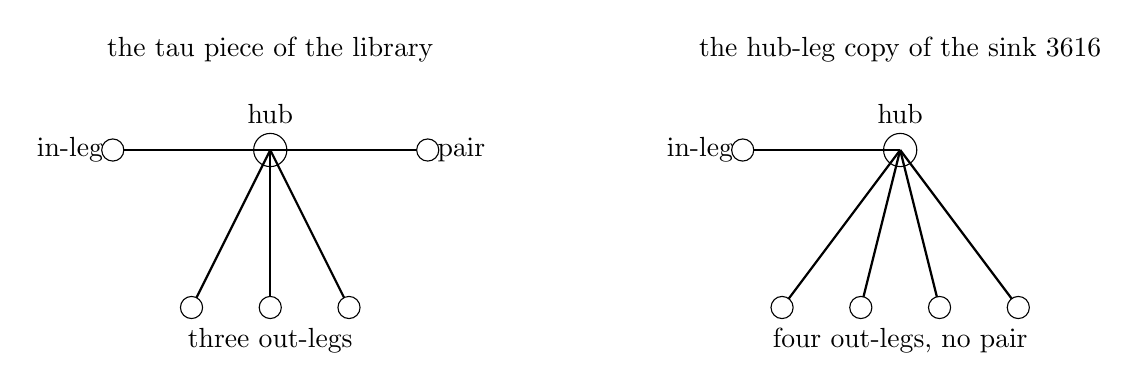
\begin{tikzpicture}[scale=1]
\filldraw[fill=white] (0,0) circle (6pt) node[above=6pt] {hub};
\draw[thick] (0,0) -- (-2,0); \filldraw[fill=white] (-2,0) circle (4pt) node[left] {in-leg};
\foreach \a in {-1,0,1} {\draw[thick] (0,0) -- (\a,-2); \filldraw[fill=white] (\a,-2) circle (4pt);}
\node at (0,-2) [below=4pt] {three out-legs};
\draw[thick] (0,0) -- (2,0); \filldraw[fill=white] (2,0) circle (4pt) node[right] {pair};
\node at (0,1) [above] {the tau piece of the library};
\filldraw[fill=white] (8,0) circle (6pt) node[above=6pt] {hub};
\draw[thick] (8,0) -- (6,0); \filldraw[fill=white] (6,0) circle (4pt) node[left] {in-leg};
\foreach \a in {65mm,75mm,85mm,95mm} {\draw[thick] (8,0) -- (\a,-2); \filldraw[fill=white] (\a,-2) circle (4pt);}
\node at (8,-2) [below=4pt] {four out-legs, no pair};
\node at (8,1) [above] {the hub-leg copy of the sink 3616};
\end{tikzpicture}\caption{A hub-leg piece of the tau web of the library, an in-leg, three out-legs and a pair, beside the hub-leg copy of the first sink of the census, which carries an in-leg and four out-legs and no pair, the first parting.}\end{figure}
\end{chproof}
\section{The dressing-leg chain}\label{mod:VIII-1-D540427-the-dressing-leg-chain}
\begin{chtable}[The dressing-leg chain]\label{box:VIII-1-D540427-the-dressing-leg-chain:1}
This table is conditional on its parent results, the open results, the theorems and the instrument among them read at their grades. The dressing-leg chain at its depth: the thirteen (3,4) results, every one an established result, laid as a derivation graph by text citation with the axiom at the root, every result reached from the root at the graph adopted, thirteen of thirteen, keyed at thirteen of thirteen with no cycle at the graph adopted and at every reading, the ladder and the leg unit located at their results at five of five locators, the (3,4) cell at every result by its pinned token, the slots of the four items beyond this depth kept owed; the first unkeyed result at the hash-only reading, the Higgs-rows result, printed as the face beside; every cell a count of a copy or a citation at a passage, compared with nothing.
\end{chtable}
\chstanding{an instrument}
\chdeps{Definitions 1.1 to 1.6 and Theorems 185.1 to 185.12}{no theorem beyond it at this release}
The results that read the (3,4) genre, the in-leg from a hub to its core qutrit, are gathered into one chain and laid as a directed graph whose edges are citations: a result is the child of another when a line of its own cites the parent, or cites the axiom. Thirteen results stand on the chain, seven theorems and six open results, and the axiom is the root from which every one is reached in at most five steps. The lepton ladder, three to the count, and the hadron ladder, the cap multiplied by a power of three, together with the leg unit twelve are located at the results that spell them. Four slots are kept for items not yet at this depth, and the first result that the stricter hash-only reading cannot key is printed beside.
\begin{chbridge}
A derivation in a formal theory is a directed acyclic graph of results, each proved from foregoing ones and ultimately from the axioms, and a dependency graph of theorems is the usual way such a structure is displayed and checked \cite{Avigad2021,Weinberg1995}. The correspondence is by name.
\end{chbridge}
\begin{chproof}[instrument]
The premises of this derivation are the axiom and the six definitions of chapter~\ref{mod:FRAMEWORK}, the mass unit and the first power of the present chapter, a theorem, and the three generations as attach sites of chapter~\ref{mod:VIII-4-three-generations-as-attach-sites}, a theorem. The chain of premises runs back to the axiom through those chapters, and the longest such chain in this compendium is twelve chapters long.
The table of this chapter is the list of the thirteen results of the chain with their kind, printed in full below with the rule that produced it: every (3,4) result the item and the solution reading name is a node at its established statement. A parent edge is drawn from a node to another whenever a line of the child cites the parent by its text hash within twelve words, or cites the axiom by address, at five readings of the citation. The graph adopted keeps the text-hash and axiom citations alone. The root is the axiom at in-degree zero. The ladder and the leg unit are located by five pinned tokens at their results. The chain is complete when every node is keyed and reached from the root with no cycle.
\begin{center}\begin{adjustbox}{max width=\linewidth}\begin{tabular}{ll}\hline entry & kind \\ \hline the Higgs rows at the hub legs & a theorem \\ the Higgs office at the leg at the quartic and vacuum entries & an open result \\ the lowering dressings as the far-end dressings & a theorem \\ the dressing as the trace over a closed leg & a theorem \\ the geodesic and the tie at the dressing & an open result \\ the geodesic as the passage of the read and the tie as the far-end rule & an open result \\ the Higgs and carrier offices at their sinks & a theorem \\ the dressing as the closed legs of the passage & an open result \\ the (2,4) link read at order two & a theorem \\ the dressing as the Higgs-to-matter leg & an open result \\ hadron spectroscopy at the cap sinks & an open result \\ the chain leptons & a theorem \\ the Higgs quartic as the ratio of offices & a theorem \\ \hline \end{tabular}\end{adjustbox}\end{center}
The thirteen nodes stand at thirteen of thirteen with the (3,4) cell found by its token at every one, the parent edges number fifty-eight over the five readings, six, eleven, ten, nine and twenty-two, and twenty-six at the graph adopted, every node is keyed at thirteen of thirteen, every node is reached from the axiom with the depth five by the longest path, and the graph is acyclic at the graph adopted and at every reading; the ladder is located at two results, the hadron ladder as the cap multiplied by a power of three at the spectroscopy result and the lepton ladder as three to the count at the lowering-dressings result, and the leg unit twelve at three. Printed beside, at the hash-only reading the first unkeyed result is the Higgs-rows result and at the provenance-and-axiom reading the closed-legs result, the older results citing their parents by header and address; the six-genres census names 91 results at the (3,4) genre, 88 of them not nodes of this chain. The chain is an instrument. Its four counter-tests stand at their pinned letters at both engines: a citation planted in memory moves the acyclicity to no with a cycle of five, a result struck whole moves the first unkeyed node, a ladder locator replaced moves the locators found to four of five, and a wrong hash at the gate is excluded; its ten controls read the same, and the chain was reproduced by a second engine built apart from the first, the two equal at every cell.
\end{chproof}
\section{The dressing as the unpassed (3,4) in-legs}\label{mod:VIII-1-D540455-upil-t1}
\begin{chtheorem}[The dressing as the unpassed (3,4) in-legs]\label{box:VIII-1-D540455-upil-t1:1}
The dressing as the unpassed (3,4) in-legs: the dressing of every body, three to the number of (3,4) in-legs its passage leaves unpassed, equals the dressing of the body-alone entry at five of five. The electron, entered at its first dock, passes its one in-leg on the geodesic to its one hub, the count zero and the dressing one; the muon reaches its two hubs tied, every in-leg dressed, the count two and the dressing nine; the tau enters at a (2,2) pair and reaches its first hub through a (2,4) leg, no (3,4) in-leg passed, the count three and the dressing twenty-seven; the proton and the neutron pass the one in-leg on the geodesic to their first hub, the counts two and three and the dressings nine and twenty-seven; the in-legs, the passage and the walk at the hadron entry re-met at every body; the first partings of the passage and Higgs-to-matter-leg entries at the electron re-met by nothing here; a theorem of the passage at the definition adopted, with the control class beside failing at the engine spelling by one representation parting of the second engine at the hadron control letters alone, typed as no fault of substance.
The first face, the dressings one, nine, twenty-seven, nine and twenty-seven equal at five of five, a theorem of the passage, reads yes, the in-legs re-met at five of five, the passage re-met at five of five and the dressings equal at the exponents zero, two, three, two and three; the second face, a body parting, reads no, the first parting none.
\end{chtheorem}
\chstanding{a theorem}
\chdeps{Definitions 1.1 to 1.6 and Theorems 185.1 to 185.12}{no theorem beyond it at this release}
The dressing of a body had been read as a product of far-end dimensions over certain legs, and the foregoing entries parted over which legs, the passage entry and the Higgs-to-matter-leg entry parting first at the electron. This theorem fixes the rule: the read enters a body at the first link of its dock set in link order that is pendant at a qubit, walks the geodesic to the first-reached hubs, dresses every in-leg it reaches at a tie, and the dressing is three to the number of (3,4) in-legs it leaves unpassed, three being the far-end dimension of such a leg. At the electron the one in-leg lies on the geodesic and is passed, so the dressing is one; at the muon the two hubs are reached together and neither in-leg is passed; at the tau the entry is a pair link and the first hub is reached through a (2,4) leg, so all three in-legs stand unpassed. The five dressings so read equal the five of the body-alone entry.
\begin{chbridge}
The physical mass of a charged lepton is its bare mass dressed by its self-interaction, and in the Standard Model the three charged leptons are three copies of one field with three Yukawa couplings and no rule relating them \cite{Weinberg1967,Peskin1995}. The correspondence is by name.
\end{chbridge}
\begin{chproof}[exhaustive census]
The premises of this derivation are the axiom and the six definitions of chapter~\ref{mod:FRAMEWORK}, the mass unit and the first power of the present chapter, a theorem, the body-alone office rule of chapter~\ref{mod:VIII-2-body-alone-office-rule}, a theorem, the lepton ladder as hub assemblies of chapter~\ref{mod:V-10-lepton-ladder-as-hub-assemblies}, a theorem, and the three generations as attach sites of chapter~\ref{mod:VIII-4-three-generations-as-attach-sites}, a theorem. The chain of premises runs back to the axiom through those chapters, and the longest such chain in this compendium is twelve chapters long.
By exhaustive enumeration of the thirteen (3,4) in-legs of the five bodies, the in-leg a (3,4) link at a hub, a site of dimension four at degree three or more, its far end the qutrit: the electron has the one in-leg $HA$. The muon has $HA$ and $H_{2}B$. The tau has $HA$, $H_{2}B$ and $H_{3}C$. The proton has $s_{3}s_{7}$, $s_{4}s_{7}$ and $s_{5}s_{7}$ at the hub $s_{7}$. The neutron has $HQ_{1}$, $HQ_{2}$, $HQ_{3}$ and $Q_{2}F$ at the hubs $H$ and $F$. Every one stands at the leg register twelve. The property tested at each in-leg is whether the passage, entered at the first dock-set link in link order pendant at a qubit, stopping at the first-reached hubs with every in-leg dressed at a tie, passes it; the counts by body are the unpassed in-legs zero, two, three, two and three, and the dressings
\begin{equation} 3^{0} = 1, \qquad 3^{2} = 9, \qquad 3^{3} = 27, \qquad 3^{2} = 9, \qquad 3^{3} = 27, \end{equation}
equal to the dressings of the body-alone entry at five of five, the first parting none, and equal to the passage, geodesic-and-tie, closed-legs and Higgs-to-matter-leg cells at twenty of twenty. The smallest case worked is the electron: entered at the pendant qubit $w_{1}$, its steps run $w_{1}$ at zero, $B$ at one, $A$ and $C$ at two, $H$ and $w_{2}$ at three, the stop at $H$ at the third step, the geodesic through $AB$, $HA$ and $Bw_{1}$, so the one in-leg $HA$ is passed and the dressing is one. Beside, the sixty-four words of the fixed library at the same walk give the exponent defined at nineteen, the dressings one at nine, nine at seven and twenty-seven at three, no dock at thirty-eight and no hub at seven, printed and deciding nothing.
The counter-tests alter the construction singly and read what moves. Reversing the tie passes both in-legs of the muon and moves its dressing to one and the first body to the muon. Entering at the last dock moves the stops and the passed legs with the dressings moving at no body. Taking the base at the hub dimension moves the dressings to one, sixteen, sixty-four, sixteen and sixty-four. Striking the axiom text unmeets the gate. Each alteration moves the cells it names, four of four. The result was reproduced by an independent route, two engines built apart, a map route against the second route, equal at every cell of the item; the controls read the same at seventeen of twenty at both engines and twenty of twenty at the first, the three apart being one representation parting of the second engine at the hadron control letters, a sorted string of name-and-step pairs against the site names, moving no cell and typed as no fault of substance. The machine-checked package named at the reproducibility appendix certifies the statements of this chapter under the definitions of this compendium and proves no theorem of the literature.
\chcert{13}
\end{chproof}
\section{The five mass-unit spellings at the (2,2) office}\label{mod:VIII-1-D542746-the-five-mass-unit-spellings-at-the-two-two-office}
\begin{chtable}[The five mass-unit spellings at the (2,2) office]\label{box:VIII-1-D542746-the-five-mass-unit-spellings-at-the-two-two-office:1}
This table is conditional on its parent results, the open results and the theorem read at their grades. The five mass-unit spellings at the (2,2) office at this depth: the five elements, one, thirty-six, sixteen, sixty-seven and sixty-seven, transcribed from the five mass-unit open results against the office of one serial (2,2) link at the seven chains at the reading adopted, equal at zero of thirty-five cells, the first face one element no and the second face the spellings that part, every one of the five at every one of the seven chains, printed with the spellings beside and the readings beside; the controls the same at fourteen of fourteen, the counter-tests at their pinned letters four of four.
\end{chtable}
\chstanding{an instrument}
\chdeps{Definitions 1.1 to 1.6 and Theorems 185.1 to 185.12}{no theorem beyond it at this release}
Five foregoing open results each spelled the mass unit as a cell, the tick at the one tick as one, the whole rung register as thirty-six, the common-support register of the electron dock as sixteen, the dock-struck unit as sixty-seven, and the first power at the probe hub leg as sixty-seven. A subsequent theorem read the tick as the office of one serial (2,2) link at each chain, an element of the field with a root-two part. This table sets the five spellings against that office at the seven chains and finds that none equals it anywhere, so no one of the five spellings is the office and the mass unit stays a question of which cell is meant; the table feeds the unit chapter.
\begin{chbridge}
The unit of mass in a physical theory is a convention fixed by a chosen standard, and in particle physics the electron mass or the electronvolt serves, every other mass a pure number in that unit \cite{Weinberg1995,Jackson1998}. The correspondence is by name.
\end{chbridge}
\begin{chproof}[instrument]
The premises of this derivation are the axiom and the six definitions of chapter~\ref{mod:FRAMEWORK}, the mass unit and the first power of the present chapter, a theorem, and the tick scale as a coupling scale of chapter~\ref{mod:X-10-tick-scale-as-a-coupling-scale}, a theorem. The chain of premises runs back to the axiom through those chapters, and the longest such chain in this compendium is twelve chapters long.
The table of this chapter is printed in full below with the rule that produced it: each of the five mass-unit open results is transcribed at its cell from its copy, the element it spells as the unit at its own face; the office of one serial (2,2) link is read as the tick entry carries it at every chain at the reading adopted, the increment read as an office; each spelling is compared with the office at each of the seven chains and read equal or parting, exactly.
\begin{center}\begin{adjustbox}{max width=\linewidth}\begin{tabular}{llll}\hline spelling & the open result it comes from & element & against the office at the seven chains \\ \hline the tick at the one tick & the mass unit at the one tick & $1$ & parts at seven of seven \\ the whole rung register & the mass unit as the rung register & $36$ & parts at seven of seven \\ the common-support register of the electron dock & the mass unit as the office at the common support & $16$ & parts at seven of seven \\ the dock-struck unit & the mass-unit spelling as a theorem & $67$ & parts at seven of seven \\ the first power at the probe hub leg & the mass-unit spelling at the probe hub leg & $67$ & parts at seven of seven \\ \hline \end{tabular}\end{adjustbox}\end{center}
The office of one serial (2,2) link at the seven chains is $\tfrac{536569}{972} + \tfrac{25}{1458}\sqrt{2}$ at the electron, $\tfrac{847609}{12} + \tfrac{25}{18}\sqrt{2}$ at the muon, $\tfrac{3475947}{4} + \tfrac{25}{2}\sqrt{2}$ at the tau, zero at the proton and at the neutron, $\tfrac{202201}{972} + \tfrac{25}{1458}\sqrt{2}$ at the photon word and $\tfrac{917593}{12} + \tfrac{25}{18}\sqrt{2}$ at the body of the universe web, so the first parting of every spelling is at the electron chain, one, thirty-six, sixteen, sixty-seven and sixty-seven against $\tfrac{536569}{972} + \tfrac{25}{1458}\sqrt{2}$; the thirteen spellings beside and the three readings beside give 648 cells, equal at none. The table is an instrument. Its four counter-tests stand at their pinned letters at both engines: a spelling replaced by the office in memory moves two cells to equal, the office at one chain replaced by the rung register moves twelve cells, the office filled with the tick at every chain and reading moves 216 cells, and a wrong hash at the gate is excluded; its fourteen controls read the same, and the table was reproduced by a second engine built apart from the first, the two equal at every cell.
\end{chproof}
\section{The six dressings at the six genres}\label{mod:VIII-1-D542965-w-sxdr}
\begin{chwall}[The six dressings at the six genres]\label{box:VIII-1-D542965-w-sxdr:1}
The alpha machinery run at the six genres refuses at no genre and prints one exact element of the ring at every genre with a qubit far end and two exact elements, one at each spelling of the closure sector, at every genre beyond it, the first parting the (3,3) genre: the pole is printed at every genre, the center acting at the mixed genres and not at the homogeneous genres, the unit functional holding the one-link identity at 48 of 48 paths at every genre, the closed reads empty at every open form, the pole at the order one at (2,2) and (2,3) and at the order two at the four dark genres, equal to the readability entry at six of six; the dressing at the package spelling is $\tfrac{30 + 30\sqrt{2}}{2304}$, $\tfrac{79 + 48\sqrt{2} + 42\sqrt{3} + 3\sqrt{6}}{31104}$, $\tfrac{450 + 96\sqrt{2}}{184320}$, $\tfrac{208 + 200\sqrt{3}}{419904}$, $\tfrac{685 + 256\sqrt{3}}{2488320}$ and $\tfrac{2100}{14745600}$, and at the count-law spelling $\tfrac{268 + 200\sqrt{3}}{419904}$, $\tfrac{685 + 296\sqrt{3}}{2488320}$ and $\tfrac{2460}{14745600}$ at the three genres where the spellings part, the closure sector 8 against 28, 8 against 28 and 15 against 105; the dressing per unit equals the dressing at every genre at both readings; the six elements equal the established columns at (2,2) and (2,3) and differ at (2,4), (3,3), (3,4) and (4,4), the first differing column (2,4); both faces printed, no observed value anywhere, compared with nothing.
The first face, six exact elements of one ring printed, reads no, the machinery printing one element at the three genres with a qubit far end and two at the three genres beyond, the genres at one element three of six; the second face, the genre at which the machinery refuses named, reads no, no step refusing at any genre, the first refusing genre none. Open is the closure sector at a qutrit or ququart far end: the polynomial spelling of the package counts the closure records as the commutators of the three far-end letters of a qubit, three at every qubit far end, and the count law of the six genres counts the pairs of the far-end letters, so the two coincide wherever the far end is a qubit and part wherever it is not, first at the (3,3) genre, and this result lays neither spelling.
\end{chwall}
\chstanding{an open result}
\chdeps{Definitions 1.1 to 1.6 and Theorems 185.1 to 185.12}{no theorem beyond it at this release}
The machinery that derives the fine-structure constant at the one (2,3) link, the identification algebra with its center, the Ward read at the unit functional, the census of the records of two reads with their weights, the register and the unit, is run unchanged at each of the six genres of the link. At every genre every step goes through: the algebra closes with a one-line center, the unit functional holds the identity, every weight is a root in the ring and the register is positive. The one ambiguity is the closure sector of the census, which the package spells by a polynomial in the far-end dimension and the count law of the six genres spells by the pairs of the far-end letters; at a qubit far end both give three and the dressing is one element, at a qutrit or ququart far end they give eight against twenty-eight or fifteen against one hundred and five and the dressing is one of two elements. The open result prints both at the three parting genres and lays neither.
\begin{chbridge}
The coupling of a gauge theory is one number at each gauge group, the fine-structure constant for the abelian group and the strong coupling for the color group, and the running of each is governed by its own beta function with a universal form across the groups \cite{Peskin1995,Gross1973}. The correspondence is by name.
\end{chbridge}
\begin{chproof}[finite computation with its census and its exact part]
The premises of this derivation are the axiom and the six definitions of chapter~\ref{mod:FRAMEWORK}, the mass unit and the first power of the present chapter, a theorem, the link and its six genres of chapter~\ref{mod:I-2-link-and-its-six-genres}, a theorem, the fine-structure constant at the one link of chapter~\ref{mod:V-1-fine-structure-constant-at-the-one-link}, a theorem, and the Ward functional and the dressing per unit of that chapter, an open result. The chain of premises runs back to the axiom through those chapters, and the longest such chain in this compendium is twelve chapters long.
\textit{The objects.} The six genres of the link are (2,2), (2,3), (2,4), (3,3), (3,4) and (4,4) at their end dimensions, each with its pair ket on the common support of two, two, two, three, three and four directions and its identification algebra of 7, 12, 19, 17, 24 and 31 elements with the brackets closed at 49, 144, 361, 289, 576 and 961 and the center one line at the primitive diagonal, $1,1,-1,-1$ at (2,2), $3,3,-2,-2,-2$ at (2,3) and $2,2,-1,-1,-1,-1$ at (2,4) among them. The figure draws the six links.
\textit{The procedure.} At each genre, re-derive the algebra and its center and read the center on the pair ket, acting or not. Re-implement the Ward read at the eight orderings and forty-eight paths and test the unit functional. Census the records of two reads by the polynomials of the package at the traceless dimensions of the two ends, three and three at (2,2), eight and three at (2,3), fifteen and three at (2,4), eight and eight at (3,3), fifteen and eight at (3,4) and fifteen and fifteen at (4,4), in the odd, mixed-even and same-even sectors, and the closure sector at both spellings, the polynomial of the package and the count law of the six genres by locator. Weight the records by the exchanges and sum over the register, the cut register multiplied by the whole register squared, for the dressing. Read the unit at the pair ket and per record and divide for the dressing per unit. Compare the six elements with the established columns.
\textit{The exact part and the smallest instance.} The records number 57, 172, 417, 392 against 412, 777 against 797 and 1365 against 1455 at the six genres, the closure sector at the two spellings 3, 3, 3, 8 against 28, 8 against 28 and 15 against 105. At the first parting genre (3,3) the register is $419904 = 64\cdot 81\cdot 81$ and the two dressings read
\begin{equation} D_{33}^{\mathrm{package}} = \frac{208 + 200\sqrt{3}}{419904}, \qquad D_{33}^{\mathrm{count\ law}} = \frac{268 + 200\sqrt{3}}{419904}, \end{equation}
the difference the sixty closure records of the count law beyond the eight of the polynomial at the weight one; at (3,4) the two read $\tfrac{685 + 256\sqrt{3}}{2488320}$ and $\tfrac{685 + 296\sqrt{3}}{2488320}$ and at (4,4) $\tfrac{2100}{14745600}$ and $\tfrac{2460}{14745600}$, while at (2,2), (2,3) and (2,4) the one element is $\tfrac{30 + 30\sqrt{2}}{2304}$, $\tfrac{79 + 48\sqrt{2} + 42\sqrt{3} + 3\sqrt{6}}{31104}$ and $\tfrac{450 + 96\sqrt{2}}{184320}$. The unit functional at the pair ket reads one, five sixths, three quarters, two thirds, seven twelfths and one half at the six genres and two per record at the sector level, and the dressing per unit equals the dressing at every genre at both readings. The pole stands at the order one at (2,2) and (2,3) and at the order two at the four dark genres, equal to the readability entry at six of six.
\textit{The census.} By exhaustive enumeration of the six genres at every step of the machinery: the property tested is whether a step refuses, the algebra not closing or its center not one line, the unit functional not holding, a weight outside the ring, the register not positive or the unit zero; the count of refusing genres is none, and the count of genres printed at one element is three of six, the first parting (3,3). The six elements equal the established columns at (2,2) and (2,3) and differ at (2,4), (3,3), (3,4) and (4,4), the first differing column (2,4).
\textit{The check.} The counter-tests alter the construction singly and read what moves. Striking the center moves the central element to zero at every genre and the machinery refuses at (2,2) at the algebra step. Swapping the ends negates the pair scalar at the mixed genres. Reading a dimension-five end refuses at the Ward read, an end outside the alphabet and a weight outside the ring. Reading the count at the record level refuses at every genre but (2,3). Striking the text unmeets the gate. Each alteration moves the cells it names, five of five. The result was reproduced by an independent route, two engines built apart, a map-and-fraction route against the second route, equal at every cell, with the fourteen controls the same.
\chcert{6}
\begin{figure}[h]\centering\begin{adjustbox}{max width=\linewidth}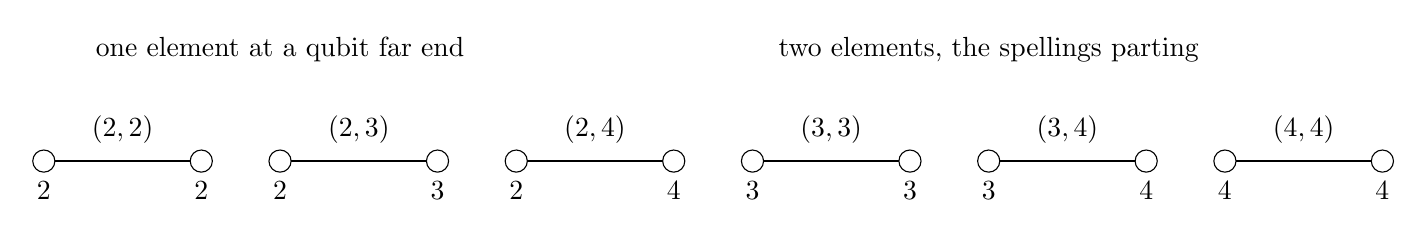
\begin{tikzpicture}[scale=1]
\foreach \x/\a/\b/\g in {0/2/2/{(2,2)}, 3/2/3/{(2,3)}, 6/2/4/{(2,4)}, 9/3/3/{(3,3)}, 12/3/4/{(3,4)}, 15/4/4/{(4,4)}} {\draw[thick] (\x,0) -- (\x+2,0); \filldraw[fill=white] (\x,0) circle (4pt) node[below=4pt] {$\a$}; \filldraw[fill=white] (\x+2,0) circle (4pt) node[below=4pt] {$\b$}; \node at (\x+1,0) [above=3pt] {$\g$};}
\node at (3,1) [above=4pt] {one element at a qubit far end};
\node at (12,1) [above=4pt] {two elements, the spellings parting};
\end{tikzpicture}\end{adjustbox}\caption{The six genres of the link with their end dimensions; at the three with a qubit far end the two spellings of the closure sector coincide and the dressing is one element, at the three beyond they part.}\end{figure}
\end{chproof}
\section{The office as a formula in the membership counts}\label{mod:VIII-1-D543206-w-ofmc}
\begin{chwall}[The office as a formula in the membership counts]\label{box:VIII-1-D543206-w-ofmc:1}
The formula in the six counts misses an established office, the first the W word: with $n$ the membership vector over the six genres, $s$ the struck vector, $k$ the dressing exponent, $m_{g}$ the weight of the genre and $G_{2,g}$ its second-order readout at the larger dimension, the formula $F(n; s, k) = 9^{k}\big\{\big(\sum_{g} m_{g}(n_{g} - s_{g})\big)^{2} + \sum_{g\ \mathrm{dark}} (n_{g} - s_{g})\, m_{g}^{2}\, G_{2,g}^{2}\big\}$ with $G_{2,g}$ per genre at the larger dimension is met at nineteen of twenty-six reads and missed first at the W word, the parting the closure at the (2,4) genre, $\tfrac{6137}{3645000} + \tfrac{4}{6075}\sqrt{2}$ against $\tfrac{10241}{3645000} + \tfrac{98}{50625}\sqrt{2}$; at the slot reading of the readout, per link at the end of larger degree and no function of the counts alone, the formula meets twenty-two of twenty-six; the first face unmet at the reading adopted, the second face met with the first body named with both cells; every cell an exact element of the field of root two and root three compared with nothing.
The first face, one formula in the six counts meeting every established office so that the spectrum is the membership table multiplied by the cell dressings and the hadron, lepton and cross-core open results become instances of one formula with their partings located at a count, reads no, the formula met at nineteen of twenty-six; the second face, the first body the formula misses named with both cells, reads yes at the W word, the parting located at the (2,4) closure. Open is the closure as a function of the counts: the per-genre closure of the formula at the larger-dimension slot parts from the per-link closure at the slot of larger degree wherever a dark link is slotted at its smaller end, and the formula at the slot reading meets that body.
\end{chwall}
\chstanding{an open result}
\chdeps{Definitions 1.1 to 1.6 and Theorems 185.1 to 185.12}{no theorem beyond it at this release}
The body-alone rule reads the office of a body link by link, the first power as a weighted count of its unstruck links, the closure as a sum over its dark links of the squared act multiplied by the second-order readout. This entry asks whether the office is a closed form in six numbers alone, the membership counts of the links by genre, with the struck links and the dressing exponent as the two indices. For nineteen of the twenty-six reads it is. It fails first at the W word of the fixed library, whose two (2,4) legs are slotted at their qubit end, so that the per-link readout at the slot of larger degree differs from the readout the formula assigns to the (2,4) genre at its larger dimension; the first power 28 and its square 784 agree, the closures do not. The parting is a matter of the slot of a dark link and not of the counts, and the three dressing open results of the chapter are re-read as instances of the formula at a count.
\begin{chbridge}
A mass formula in particle physics expresses the masses of a multiplet in terms of a few quantum numbers and parameters, the Gell-Mann and Okubo formula for the baryon octet the standard example, with the residual splittings attributed to interactions the formula omits \cite{GellMann1962,Okubo1962}. The correspondence is by name.
\end{chbridge}
\begin{chproof}[finite computation with its census]
The premises of this derivation are the axiom and the six definitions of chapter~\ref{mod:FRAMEWORK}, the mass unit and the first power of the present chapter, a theorem, the body-alone office rule of chapter~\ref{mod:VIII-2-body-alone-office-rule}, a theorem, the Higgs and carrier offices at their sinks of chapter~\ref{mod:VI-10-higgs-the-closed-hub-read-its-rows-its-mass-and-its-exponent}, a theorem, and the dressing as the unpassed (3,4) in-legs of the present chapter, a theorem. The chain of premises runs back to the axiom through those chapters, and the longest such chain in this compendium is twelve chapters long.
\textit{The procedure.} The input objects are the twenty-six reads, eight of the Higgs-and-carrier-offices entry at the measure-struck reading, seven of the body-alone entry at the segment reading, six of the tau-web entry, two tau-form sinks of the lepton-sink entry and three of the cross-core entry, each with its office under the rule re-met at every link, every link at its weight, the product of the end dimensions, the dock set struck, the dressing the far-end product over the in-legs at hubs, and the closure at a dark link the square of the act multiplied by the second-order readout at its slot. For each read form the membership vector $n$ over the genres (2,2), (2,3), (2,4), (3,3), (3,4) and (4,4), the struck vector $s$ and the exponent $k$, and evaluate the formula with the weights $m_{g}$ of 4, 6, 8, 9, 12 and 16 and the readouts at the larger dimension, $\tfrac{5}{216} + \tfrac{5}{216}\sqrt{2}$ at (2,2), $\tfrac{1}{288} + \tfrac{1}{1350}\sqrt{2}$ at (2,4), $\tfrac{67}{82944} + \tfrac{25}{41472}\sqrt{3}$ at (3,3), $\tfrac{137}{414720} + \tfrac{37}{259200}\sqrt{3}$ at (3,4) and $\tfrac{41}{216000}$ at (4,4), the (2,3) genre outside the dark set; compare with the office and name the first read missed.
\textit{The smallest instance.} The W word carries the membership vector $(0, 2, 2, 0, 0, 0)$, the struck vector zero and the exponent zero, so its first power is $6\cdot 2 + 8\cdot 2 = 28$ with the square $784$, and the closure term of the formula at its two dark (2,4) links is
\begin{equation} 2\cdot 8^{2}\cdot\Big(\tfrac{1}{288} + \tfrac{1}{1350}\sqrt{2}\Big)^{2} = \tfrac{6137}{3645000} + \tfrac{4}{6075}\sqrt{2}, \qquad F = 784 + \tfrac{6137}{3645000} + \tfrac{4}{6075}\sqrt{2} = \tfrac{2857686137}{3645000} + \tfrac{4}{6075}\sqrt{2}, \end{equation}
against the office $\tfrac{2857690241}{3645000} + \tfrac{98}{50625}\sqrt{2}$, whose closure $\tfrac{10241}{3645000} + \tfrac{98}{50625}\sqrt{2}$ is read per link at the slot of larger degree, the qubit end of each leg; the parting is located at the (2,4) closure and at no count.
\textit{The census.} By exhaustive enumeration of the twenty-six reads at the reading adopted, the struck vector and the exponent of the read with the readout per genre at the larger dimension: the property tested is equality of the formula with the office; the counts are met at nineteen of twenty-six, missed at seven, the W word, the Z word, the proton, the neutron through the deuteron, the strike-rule neutron, the one-link electron and the tau sink; printed beside, at the slot reading of the readout the formula meets twenty-two of twenty-six and at the pure-count reading seven of twenty-six; the 179 per-link readout cells of the reads are re-met by the count law at 179 of 179; and the three dressing open results of the chapter are re-read as instances of the formula at a count.
\textit{The check.} The counter-tests alter the construction singly and read what moves. Incrementing the struck vector at the (2,2) genre moves every read carrying an unstruck pair. Adding one (4,4) link to every membership vector moves every read and the first body missed to the Higgs word. Dropping the closure moves every read with a nonzero closure. Reading a word of the library with no office, the gluon word, holds at its cells with the formula and the rule printed and compared with nothing. Striking the gate exits at both engines. Each alteration moves the cells it names, five of five. The result was reproduced by an independent route, two engines built apart, the explicit record-space route against the second route, equal at every cell; the controls read the same at fourteen of fifteen at the pinned grammar, the fifteenth mis-posed at two reads carrying no census row and re-read holding at the census-keyed reads at twenty-four of twenty-four.
\chcert{26}
\end{chproof}
\par\medskip\noindent{\itshape The unit fixed, the next chapter says which office a body reads alone.}\label{narr:close:8-1}\par
\section{The body-alone office rule}\label{mod:VIII-2-body-alone-office-rule}
\chdesig{10-2}{8-2}{VIII-2-body-alone-office-rule}{VIII-2-body-alone-office-rule}
\label{narr:open:8-2}Theorem~195.1 is the body-alone office rule, a theorem resting on the records, the saturation and the mass unit, and the quark and carrier offices of Parts VIII and IX rest on it.
\begin{chtheorem}[The body-alone office rule]\label{box:VIII-2-body-alone-office-rule:1}
The office of every body at its own sink is defined as an exact nonzero element of the field at the five bodies: its pair part equals the first power squared of the segment theorem by the two-read identity, and its closure part is an exact cell, positive at the three leptons and zero at the proton and at the neutron through the deuteron.
\end{chtheorem}
\chstanding{theorem}
\chdeps{Definitions 1.1 to 1.6, Theorems 18.1 to 18.4 and Open results 18.5 and 18.6, Theorems 185.1 to 185.12 and Open results 245.1 and 245.2, Theorem 245.3, Open results 245.4 to 245.8 and Theorem 245.9}{the theorems of Chapters 1-1, 1-3, 1-5, 4-6, 5-3, 5-8, 5-8f, 6-2, 6-6, 9-7, 11-1, 12-1}
The reading adopted takes the act read of every link from the segment theorem, the dark set as every link of a genre other than the read genre, and the closure at a dark link as the square of its act read multiplied by the grid factor. The readings of the grid meet at every segment reading. The rule itself is the chapter. A body belongs to the force of its defining read, and the quark offices and the Higgs and carrier offices of their own chapters take this rule as their derivation.
\begin{chbridge}
The rest mass of a body is the invariant of its four-momentum, in the Standard Model a parameter of the Lagrangian for each field set by its coupling to the Higgs field and fixed by nothing within the theory, and the Born rule reads the probability of an outcome as the squared modulus of the amplitude of the transition \cite{Born1926,Dirac1928,Weinberg1967}. The correspondence is by name.
\end{chbridge}
\begin{chproof}[finite computation with its exact part]
\textit{The premises.} The axiom and the six definitions of Section~\ref{mod:FRAMEWORK}, definitions. The Born count and the gain lemma of Section~\ref{mod:I-3-records-reads-and-the-born-count-the-gain-lemma}, a theorem. The sinks of the saturation of Section~\ref{mod:I-5-saturation-in-one-figure-seeds-waves-termination-sinks}, a theorem. The mass unit and the first power of Section~\ref{mod:VIII-1-mass-unit-and-the-first-power}, a theorem. The chain from the axiom to this result is six chapters deep.

\textit{The exact part: the office of one body.} A body is read at its own sink and nowhere else. Its web has sites and links, each link of a genre given by the two end dimensions. The read enters at a dock of the read genre, the (2,3) genre, and the segment theorem assigns to every link an act read. From the act reads of the links, by summation, we obtain the first power of the body,
\begin{equation}
S_1=\sum_{\ell} a_\ell ,
\end{equation}
the sum running over the links of the web. From the first power, by the two-read identity (the sum over the ordered pairs of links of the product of their act reads equals the square of the sum), we obtain the pair part,
\begin{equation}
\mathrm{pair}=\sum_{\ell,\ell'} a_\ell a_{\ell'}=S_1^{2}.
\end{equation}
From the dark set, every link of a genre other than (2,3), and the grid factor $G_2$ of the count law at the six genres, by the closure rule of this chapter (a dark link closes at the square of its act read multiplied by the grid factor, a link read at nothing closing at nothing), we obtain the closure part,
\begin{equation}
\mathrm{closure}=\sum_{\ell\ \mathrm{dark}} a_\ell^{2}\,G_2 ,
\end{equation}
an element of the ring with basis one, root two, root three and root six. From the pair part and the closure part, by addition, we obtain the office of the body at its own sink, $\mathrm{office}=\mathrm{pair}+\mathrm{closure}$.

\textit{The smallest instance.} The one-link electron web is one (2,3) link. Its act read is the unit, $S_1=67$. The dark set is empty, so by the three displays
\begin{equation}
\mathrm{pair}=67^{2}=4489,\qquad \mathrm{closure}=0,\qquad \mathrm{office}=4489 .
\end{equation}

\textit{The finite computation at the five bodies.} The input objects are the five webs. The electron stands at its two-dock web, drawn at the figure, with ten links, the measure 79 and the dock set 12 at its two (2,3) docks. The muon stands at its web of fifteen links, the measure 117 and the dock set 10. The tau stands at its web of twenty links, the measure 155 and the dock set 8. The proton stands at the sink of the bound-respecting reading with nine links, the measure 81 and the dock set 18, its entered link capped at the cap of its genre. The neutron through the deuteron stands at the typing adopted with twenty-eight links, the measure 219 and the dock set 36, its entered link capped. The enumeration rule is the one procedure of the exact part applied to each web with no body-specific term. The test applied to each body is whether the pair part equals the first power squared and whether the closure part is an exact element of the ring. The aggregation is the office. The first powers at the natural checkpoint are
\begin{equation}
S_1=67,\ 963,\ 3969,\ 2871,\ 2871
\end{equation}
at the electron, the muon, the tau, the proton and the neutron through the deuteron, and the pair parts are their squares,
\begin{equation}
\mathrm{pair}=4489,\ 927\,369,\ 15\,752\,961,\ 8\,242\,641,\ 8\,242\,641 ,
\end{equation}
the two-read identity holding at every one of the 760 cells of the grid of readings. The closure parts at the three leptons are
\begin{align}
\mathrm{closure}_{e}&=\tfrac{13\,708\,610\,839}{477\,757\,440\,000}+\tfrac{661}{36\,450}\sqrt{2}+\tfrac{5\,977\,541}{23\,887\,872\,000}\sqrt{3}\quad\text{at eight dark links},\\
\mathrm{closure}_{\mu}&=\tfrac{27\,214\,907\,303}{5\,898\,240\,000}+\tfrac{661}{225}\sqrt{2}+\tfrac{6\,301\,957}{294\,912\,000}\sqrt{3}\quad\text{at fourteen dark links},\\
\mathrm{closure}_{\tau}&=\tfrac{40\,721\,203\,767}{655\,360\,000}+\tfrac{1983}{50}\sqrt{2}+\tfrac{6\,626\,373}{32\,768\,000}\sqrt{3}\quad\text{at twenty dark links},
\end{align}
each positive, and at the proton and at the neutron through the deuteron the closure part is zero, every dark link beyond the first cap being read at nothing (six dark links at the proton, twenty-two at the neutron through the deuteron). From the pair parts and the closure parts, by addition, we obtain the offices
\begin{align}
\mathrm{office}_{e}&=\tfrac{2\,144\,666\,856\,770\,839}{477\,757\,440\,000}+\tfrac{661}{36\,450}\sqrt{2}+\tfrac{5\,977\,541}{23\,887\,872\,000}\sqrt{3},\\
\mathrm{office}_{\mu}&=\tfrac{5\,469\,872\,145\,467\,303}{5\,898\,240\,000}+\tfrac{661}{225}\sqrt{2}+\tfrac{6\,301\,957}{294\,912\,000}\sqrt{3},\\
\mathrm{office}_{\tau}&=\tfrac{10\,323\,901\,242\,163\,767}{655\,360\,000}+\tfrac{1983}{50}\sqrt{2}+\tfrac{6\,626\,373}{32\,768\,000}\sqrt{3},\\
\mathrm{office}_{p}&=\mathrm{office}_{n}=8\,242\,641 ,
\end{align}
every one an exact nonzero element of the field, which is the statement. The ratio of the proton office to the one-link electron office is the exact cell $8\,242\,641/4489$, the Born-square ratio of the neutron result re-met.

\textit{The check.} Striking the closure records at the muon moves the muon office. Reading a dark link at first order, so that the dark set of the electron is empty, moves the electron closure. Leaving the dock of the electron unstruck moves the electron pair part away from the first power squared. Lifting the cap at the proton moves the proton pair part away from the first power squared. Each alteration moves the cell it names and nothing else. The result was reproduced by an independent route, a map-and-fraction route and an array-scan big-integer route agreeing at every deciding cell at both runs, with the two-read identity as the control at every cell of the grid. The derivation follows the spelling of the mass result and of the neutron result, which it cites as its precedents.
\chcert{80}
\end{chproof}
\begin{figure}[H]\centering
\begin{tikzpicture}[x=0.52pt,y=-0.52pt,baseline]
\clip (0,0) rectangle (900,540);
\fill[white] (0,0) rectangle (900,540);
\node[anchor=base west,inner sep=0pt,text=black,font=\fontsize{6.76}{8.112}\selectfont\ttfamily] at (12,22) {atlas body-alone:E1: one-link-web};
\node[anchor=base west,inner sep=0pt,text=black,font=\fontsize{6.24}{7.488}\selectfont\ttfamily] at (12,42) {membership 22:0;23:1;24:0;33:0;34:0;44:0; cells (2,3); links 1; sites 2; measure 6; census at the census};
\node[anchor=base west,inner sep=0pt,text=black,font=\fontsize{5.72}{6.864}\selectfont\ttfamily] at (12,62) {recorded office body-alone:E1:segment/R1/weight:E1=4489\textbar{}0\textbar{}0\textbar{}0; standing census:instrument;body-alone:theorem;formula:open result; board none};
\draw[draw=black,line width=1.04pt,dash pattern=on 1.04pt off 1.56pt] (100,470) .. controls (130,450) and (160,450) .. (190,470);
\node[anchor=base,inner sep=0pt,text=black,font=\fontsize{5.72}{6.864}\selectfont\ttfamily] at (145,451) {(2,3)};
\filldraw[fill={rgb,255:red,244;green,192;blue,192},draw=black,line width=0.52pt] (100,470) circle (14);
\node[anchor=base,inner sep=0pt,text=black,font=\fontsize{6.24}{7.488}\selectfont\ttfamily] at (100,475) {0};
\node[anchor=base,inner sep=0pt,text=black,font=\fontsize{5.72}{6.864}\selectfont\ttfamily] at (100,500) {x2};
\filldraw[fill={rgb,255:red,244;green,192;blue,192},draw=black,line width=0.52pt] (190,470) circle (14);
\node[anchor=base,inner sep=0pt,text=black,font=\fontsize{6.24}{7.488}\selectfont\ttfamily] at (190,475) {0};
\node[anchor=base,inner sep=0pt,text=black,font=\fontsize{5.72}{6.864}\selectfont\ttfamily] at (190,500) {x3};
\node[anchor=base west,inner sep=0pt,text=black,font=\fontsize{5.72}{6.864}\selectfont\ttfamily] at (12,510) {the sites labelled by register (2 the qubit, white; 3 the qutrit, grey; 4 the ququart, dark); the links labelled by cell (p,q); a long dash an open dark link of the neutron row; a short dash a docked link at the rule R1};
\end{tikzpicture}
\caption{\texttt{one-link-web}, one link web: 2 sites, 1 links, the measure 6; the links at the cells (2,3); the membership 22:0; 23:1; 24:0; 33:0; 34:0; 44:0; 1 docked links at the rule R1 (x3-x2); at the census of the six cells; 2 sites at the fourth band with the register unresolved by the genre alone, the drawing gloss not drawn at them as the compendium prints it. Drawn at the anatomy atlas as its web, the sites labeled by register and the links by cell, from the the body-alone office rule.}\label{fig:VIII-2-D537322-one-link-web-1d74cd}
\begin{center}\footnotesize\begin{adjustbox}{max width=\linewidth}\begin{tabular}{p{0.26\textwidth}p{0.68\textwidth}}\toprule
recorded office (the slot-count row) & the read O-E1 of the formula row: the first power 67; the office \texttt{4489\textbar{}0\textbar{}0\textbar{}0}; against the formula with the slot count equal; the slot total 0; dark links 0; hubs none; dressing 1 \\
mass register (the mass-register row) & the read BE1: the class within the qubit and the qutrit; the first power 0; the office \texttt{0\textbar{}0\textbar{}0\textbar{}0}; zero; met yes; hubs none; in-legs none; dressing 1; ports x3-x2 \\
\bottomrule\end{tabular}\end{adjustbox}\end{center}
\end{figure}
\begin{figure}[H]\centering
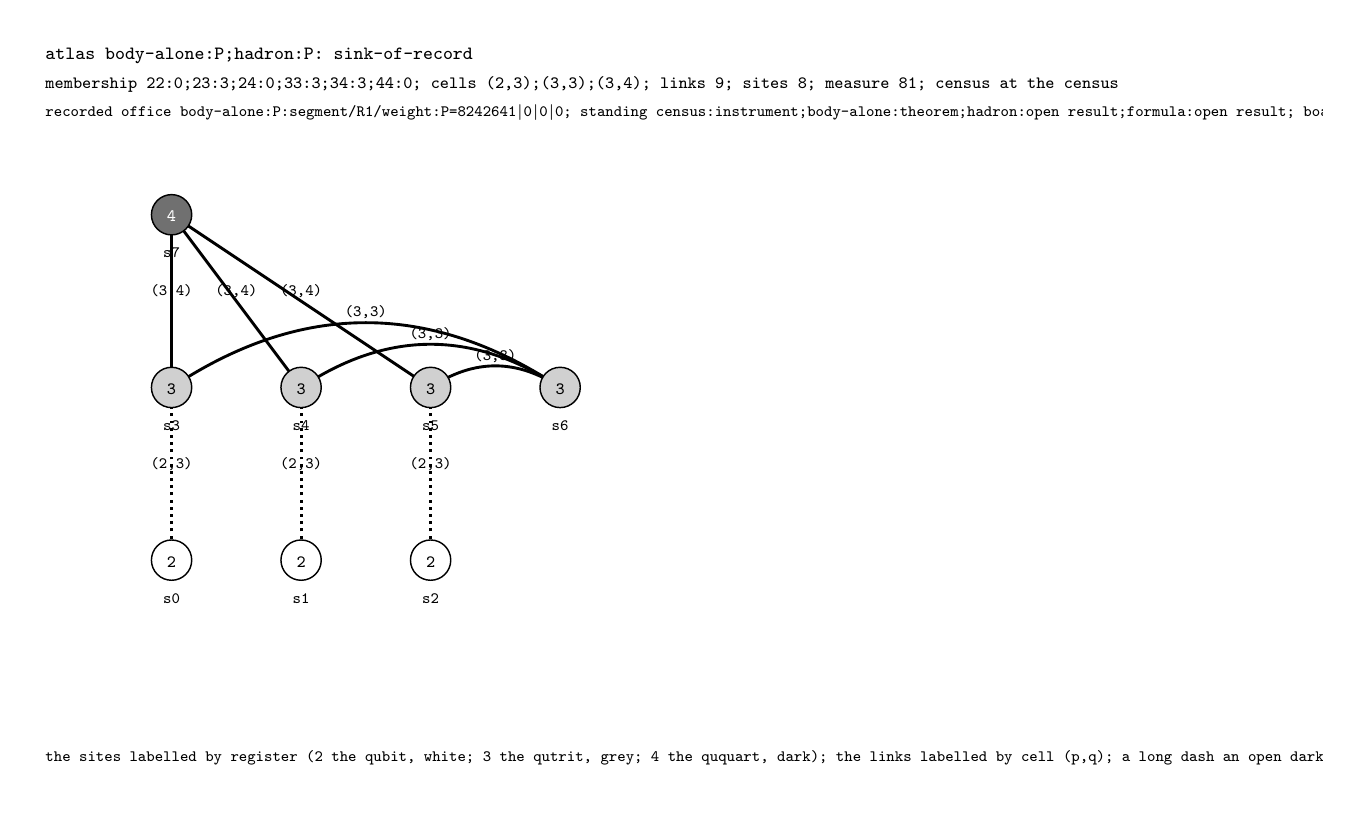
\begin{tikzpicture}[x=0.52pt,y=-0.52pt,baseline]
\clip (0,0) rectangle (900,540);
\fill[white] (0,0) rectangle (900,540);
\node[anchor=base west,inner sep=0pt,text=black,font=\fontsize{6.76}{8.112}\selectfont\ttfamily] at (12,22) {atlas body-alone:P;hadron:P: sink-of-record};
\node[anchor=base west,inner sep=0pt,text=black,font=\fontsize{6.24}{7.488}\selectfont\ttfamily] at (12,42) {membership 22:0;23:3;24:0;33:3;34:3;44:0; cells (2,3);(3,3);(3,4); links 9; sites 8; measure 81; census at the census};
\node[anchor=base west,inner sep=0pt,text=black,font=\fontsize{5.72}{6.864}\selectfont\ttfamily] at (12,62) {recorded office body-alone:P:segment/R1/weight:P=8242641\textbar{}0\textbar{}0\textbar{}0; standing census:instrument;body-alone:theorem;hadron:open result;formula:open result; board proton};
\draw[draw=black,line width=1.04pt,dash pattern=on 1.04pt off 1.56pt] (100,370) -- (100,250);
\node[anchor=base,inner sep=0pt,text=black,font=\fontsize{5.72}{6.864}\selectfont\ttfamily] at (100,306) {(2,3)};
\draw[draw=black,line width=1.04pt,dash pattern=on 1.04pt off 1.56pt] (190,370) -- (190,250);
\node[anchor=base,inner sep=0pt,text=black,font=\fontsize{5.72}{6.864}\selectfont\ttfamily] at (190,306) {(2,3)};
\draw[draw=black,line width=1.04pt,dash pattern=on 1.04pt off 1.56pt] (280,370) -- (280,250);
\node[anchor=base,inner sep=0pt,text=black,font=\fontsize{5.72}{6.864}\selectfont\ttfamily] at (280,306) {(2,3)};
\draw[draw=black,line width=1.04pt] (100,250) .. controls (190,190) and (280,190) .. (370,250);
\node[anchor=base,inner sep=0pt,text=black,font=\fontsize{5.72}{6.864}\selectfont\ttfamily] at (235,201) {(3,3)};
\draw[draw=black,line width=1.04pt] (100,250) -- (100,130);
\node[anchor=base,inner sep=0pt,text=black,font=\fontsize{5.72}{6.864}\selectfont\ttfamily] at (100,186) {(3,4)};
\draw[draw=black,line width=1.04pt] (190,250) .. controls (250,210) and (310,210) .. (370,250);
\node[anchor=base,inner sep=0pt,text=black,font=\fontsize{5.72}{6.864}\selectfont\ttfamily] at (280,216) {(3,3)};
\draw[draw=black,line width=1.04pt] (190,250) -- (100,130);
\node[anchor=base,inner sep=0pt,text=black,font=\fontsize{5.72}{6.864}\selectfont\ttfamily] at (145,186) {(3,4)};
\draw[draw=black,line width=1.04pt] (280,250) .. controls (310,230) and (340,230) .. (370,250);
\node[anchor=base,inner sep=0pt,text=black,font=\fontsize{5.72}{6.864}\selectfont\ttfamily] at (325,231) {(3,3)};
\draw[draw=black,line width=1.04pt] (280,250) -- (100,130);
\node[anchor=base,inner sep=0pt,text=black,font=\fontsize{5.72}{6.864}\selectfont\ttfamily] at (190,186) {(3,4)};
\filldraw[fill=white,draw=black,line width=0.52pt] (100,370) circle (14);
\node[anchor=base,inner sep=0pt,text=black,font=\fontsize{6.24}{7.488}\selectfont\ttfamily] at (100,375) {2};
\node[anchor=base,inner sep=0pt,text=black,font=\fontsize{5.72}{6.864}\selectfont\ttfamily] at (100,400) {s0};
\filldraw[fill=white,draw=black,line width=0.52pt] (190,370) circle (14);
\node[anchor=base,inner sep=0pt,text=black,font=\fontsize{6.24}{7.488}\selectfont\ttfamily] at (190,375) {2};
\node[anchor=base,inner sep=0pt,text=black,font=\fontsize{5.72}{6.864}\selectfont\ttfamily] at (190,400) {s1};
\filldraw[fill=white,draw=black,line width=0.52pt] (280,370) circle (14);
\node[anchor=base,inner sep=0pt,text=black,font=\fontsize{6.24}{7.488}\selectfont\ttfamily] at (280,375) {2};
\node[anchor=base,inner sep=0pt,text=black,font=\fontsize{5.72}{6.864}\selectfont\ttfamily] at (280,400) {s2};
\filldraw[fill={rgb,255:red,208;green,208;blue,208},draw=black,line width=0.52pt] (100,250) circle (14);
\node[anchor=base,inner sep=0pt,text=black,font=\fontsize{6.24}{7.488}\selectfont\ttfamily] at (100,255) {3};
\node[anchor=base,inner sep=0pt,text=black,font=\fontsize{5.72}{6.864}\selectfont\ttfamily] at (100,280) {s3};
\filldraw[fill={rgb,255:red,208;green,208;blue,208},draw=black,line width=0.52pt] (190,250) circle (14);
\node[anchor=base,inner sep=0pt,text=black,font=\fontsize{6.24}{7.488}\selectfont\ttfamily] at (190,255) {3};
\node[anchor=base,inner sep=0pt,text=black,font=\fontsize{5.72}{6.864}\selectfont\ttfamily] at (190,280) {s4};
\filldraw[fill={rgb,255:red,208;green,208;blue,208},draw=black,line width=0.52pt] (280,250) circle (14);
\node[anchor=base,inner sep=0pt,text=black,font=\fontsize{6.24}{7.488}\selectfont\ttfamily] at (280,255) {3};
\node[anchor=base,inner sep=0pt,text=black,font=\fontsize{5.72}{6.864}\selectfont\ttfamily] at (280,280) {s5};
\filldraw[fill={rgb,255:red,208;green,208;blue,208},draw=black,line width=0.52pt] (370,250) circle (14);
\node[anchor=base,inner sep=0pt,text=black,font=\fontsize{6.24}{7.488}\selectfont\ttfamily] at (370,255) {3};
\node[anchor=base,inner sep=0pt,text=black,font=\fontsize{5.72}{6.864}\selectfont\ttfamily] at (370,280) {s6};
\filldraw[fill={rgb,255:red,112;green,112;blue,112},draw=black,line width=0.52pt] (100,130) circle (14);
\node[anchor=base,inner sep=0pt,text=white,font=\fontsize{6.24}{7.488}\selectfont\ttfamily] at (100,135) {4};
\node[anchor=base,inner sep=0pt,text=black,font=\fontsize{5.72}{6.864}\selectfont\ttfamily] at (100,160) {s7};
\node[anchor=base west,inner sep=0pt,text=black,font=\fontsize{5.72}{6.864}\selectfont\ttfamily] at (12,510) {the sites labelled by register (2 the qubit, white; 3 the qutrit, grey; 4 the ququart, dark); the links labelled by cell (p,q); a long dash an open dark link of the neutron row; a short dash a docked link at the rule R1};
\end{tikzpicture}
\caption{\texttt{sink-of-record} (the proton), recorded body, hadron row body: 8 sites, 9 links, the measure 81; the links at the cells (2,3), (3,3), (3,4); the membership 22:0; 23:3; 24:0; 33:3; 34:3; 44:0; 3 docked links at the rule R1 (s0-s3; s1-s4; s2-s5); at the census of the six cells. Drawn at the anatomy atlas as its web, the sites labeled by register and the links by cell, from the the body-alone office rule.}\label{fig:VIII-2-D537322-sink-of-record-1d9538}
\begin{center}\footnotesize\begin{adjustbox}{max width=\linewidth}\begin{tabular}{p{0.26\textwidth}p{0.68\textwidth}}\toprule
recorded office (the slot-count row) & the read o-p of the formula row: the first power 2871; the office \texttt{8242641\textbar{}0\textbar{}0\textbar{}0}; against the formula with the slot count equal; the slot total 0; dark links 6; hubs s7; dressing 9 \\
mass register (the mass-register row) & the read BP: the class touching the ququart; the first power 1701; the office \texttt{1 896 219 516 813 879/655360000\textbar{}0\textbar{}6626373/32768000\textbar{}0}; nonzero; met yes; hubs s7; in-legs s3-s7; s4-s7; s5-s7; dressing 27; ports s0-s3; s1-s4; s2-s5 \\
junction registers (the hadron row) & the read P: junctions s3; s4; s5; s6; the share one third per leg; the registers at the share 81, struck 63, mono 0, the hub spelling 729; against the cells none; none; none; none, none \\
\bottomrule\end{tabular}\end{adjustbox}\end{center}
\end{figure}
\begin{figure}[H]\centering
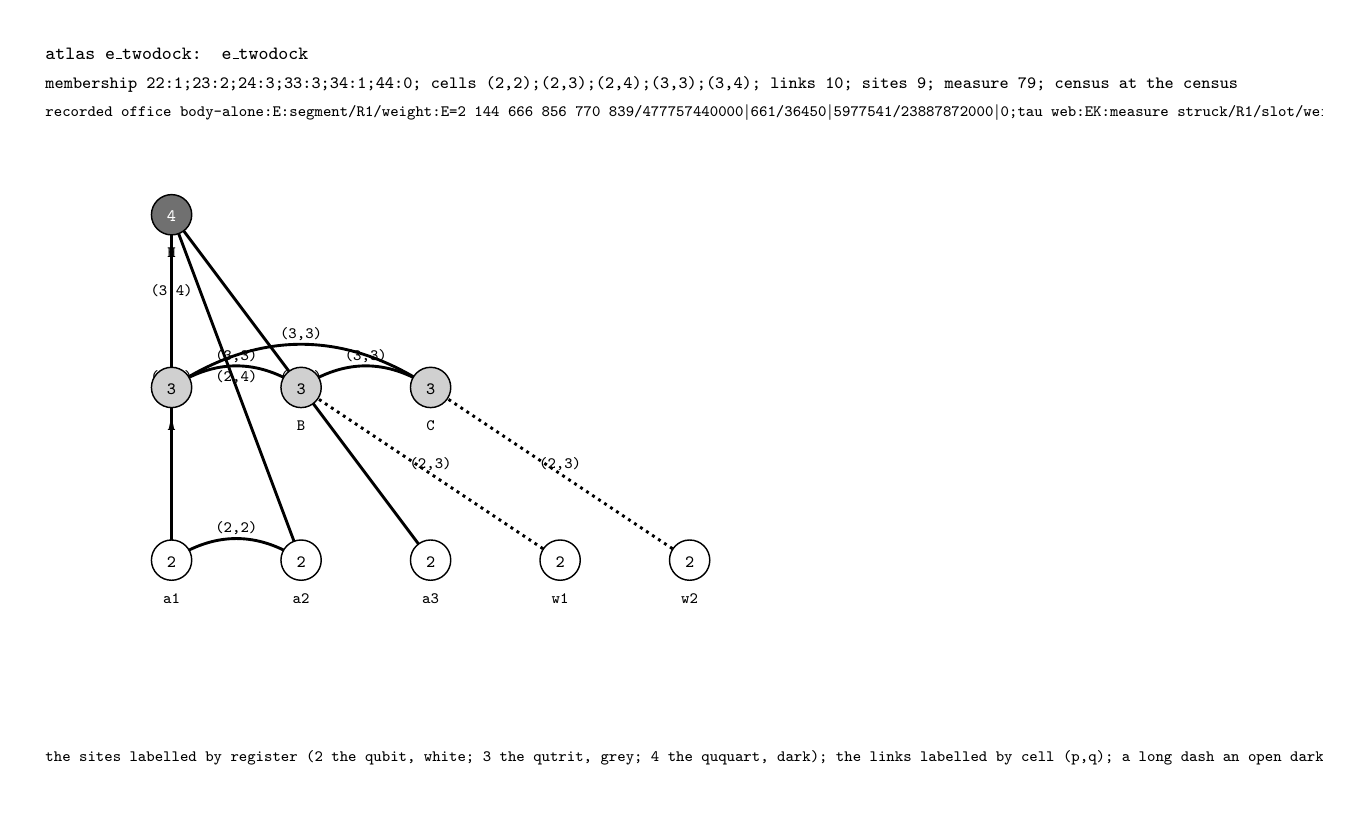
\begin{tikzpicture}[x=0.52pt,y=-0.52pt,baseline]
\clip (0,0) rectangle (900,540);
\fill[white] (0,0) rectangle (900,540);
\node[anchor=base west,inner sep=0pt,text=black,font=\fontsize{6.76}{8.112}\selectfont\ttfamily] at (12,22) {atlas e\_twodock: e\_twodock};
\node[anchor=base west,inner sep=0pt,text=black,font=\fontsize{6.24}{7.488}\selectfont\ttfamily] at (12,42) {membership 22:1;23:2;24:3;33:3;34:1;44:0; cells (2,2);(2,3);(2,4);(3,3);(3,4); links 10; sites 9; measure 79; census at the census};
\node[anchor=base west,inner sep=0pt,text=black,font=\fontsize{5.72}{6.864}\selectfont\ttfamily] at (12,62) {recorded office body-alone:E:segment/R1/weight:E=2 144 666 856 770 839/477757440000\textbar{}661/36450\textbar{}5977541/23887872000\textbar{}0;tau web:EK:measure struck/R1/slot/weight:EK=2 144 666 856 770 839/53084160000\textbar{}661/4050\textbar{}5977541/2654208000\textbar{}0; standing census:instrument;body-alone:theorem;hadron:open result;offices:theorem;nucleon:theorem;light-neutral office:theorem;formula:open result;tau web:theorem;roster:roster word; board electron};
\draw[draw=black,line width=1.04pt] (100,250) .. controls (130,230) and (160,230) .. (190,250);
\node[anchor=base,inner sep=0pt,text=black,font=\fontsize{5.72}{6.864}\selectfont\ttfamily] at (145,231) {(3,3)};
\draw[draw=black,line width=1.04pt] (100,250) .. controls (160,210) and (220,210) .. (280,250);
\node[anchor=base,inner sep=0pt,text=black,font=\fontsize{5.72}{6.864}\selectfont\ttfamily] at (190,216) {(3,3)};
\draw[draw=black,line width=1.04pt] (100,250) -- (100,130);
\node[anchor=base,inner sep=0pt,text=black,font=\fontsize{5.72}{6.864}\selectfont\ttfamily] at (100,186) {(3,4)};
\draw[draw=black,line width=1.04pt] (190,250) .. controls (220,230) and (250,230) .. (280,250);
\node[anchor=base,inner sep=0pt,text=black,font=\fontsize{5.72}{6.864}\selectfont\ttfamily] at (235,231) {(3,3)};
\draw[draw=black,line width=1.04pt,dash pattern=on 1.04pt off 1.56pt] (190,250) -- (370,370);
\node[anchor=base,inner sep=0pt,text=black,font=\fontsize{5.72}{6.864}\selectfont\ttfamily] at (280,306) {(2,3)};
\draw[draw=black,line width=1.04pt,dash pattern=on 1.04pt off 1.56pt] (280,250) -- (460,370);
\node[anchor=base,inner sep=0pt,text=black,font=\fontsize{5.72}{6.864}\selectfont\ttfamily] at (370,306) {(2,3)};
\draw[draw=black,line width=1.04pt] (100,130) -- (100,370);
\node[anchor=base,inner sep=0pt,text=black,font=\fontsize{5.72}{6.864}\selectfont\ttfamily] at (100,246) {(2,4)};
\draw[draw=black,line width=1.04pt] (100,130) -- (190,370);
\node[anchor=base,inner sep=0pt,text=black,font=\fontsize{5.72}{6.864}\selectfont\ttfamily] at (145,246) {(2,4)};
\draw[draw=black,line width=1.04pt] (100,130) -- (280,370);
\node[anchor=base,inner sep=0pt,text=black,font=\fontsize{5.72}{6.864}\selectfont\ttfamily] at (190,246) {(2,4)};
\draw[draw=black,line width=1.04pt] (100,370) .. controls (130,350) and (160,350) .. (190,370);
\node[anchor=base,inner sep=0pt,text=black,font=\fontsize{5.72}{6.864}\selectfont\ttfamily] at (145,351) {(2,2)};
\filldraw[fill={rgb,255:red,208;green,208;blue,208},draw=black,line width=0.52pt] (100,250) circle (14);
\node[anchor=base,inner sep=0pt,text=black,font=\fontsize{6.24}{7.488}\selectfont\ttfamily] at (100,255) {3};
\node[anchor=base,inner sep=0pt,text=black,font=\fontsize{5.72}{6.864}\selectfont\ttfamily] at (100,280) {A};
\filldraw[fill={rgb,255:red,208;green,208;blue,208},draw=black,line width=0.52pt] (190,250) circle (14);
\node[anchor=base,inner sep=0pt,text=black,font=\fontsize{6.24}{7.488}\selectfont\ttfamily] at (190,255) {3};
\node[anchor=base,inner sep=0pt,text=black,font=\fontsize{5.72}{6.864}\selectfont\ttfamily] at (190,280) {B};
\filldraw[fill={rgb,255:red,208;green,208;blue,208},draw=black,line width=0.52pt] (280,250) circle (14);
\node[anchor=base,inner sep=0pt,text=black,font=\fontsize{6.24}{7.488}\selectfont\ttfamily] at (280,255) {3};
\node[anchor=base,inner sep=0pt,text=black,font=\fontsize{5.72}{6.864}\selectfont\ttfamily] at (280,280) {C};
\filldraw[fill={rgb,255:red,112;green,112;blue,112},draw=black,line width=0.52pt] (100,130) circle (14);
\node[anchor=base,inner sep=0pt,text=white,font=\fontsize{6.24}{7.488}\selectfont\ttfamily] at (100,135) {4};
\node[anchor=base,inner sep=0pt,text=black,font=\fontsize{5.72}{6.864}\selectfont\ttfamily] at (100,160) {H};
\filldraw[fill=white,draw=black,line width=0.52pt] (100,370) circle (14);
\node[anchor=base,inner sep=0pt,text=black,font=\fontsize{6.24}{7.488}\selectfont\ttfamily] at (100,375) {2};
\node[anchor=base,inner sep=0pt,text=black,font=\fontsize{5.72}{6.864}\selectfont\ttfamily] at (100,400) {a1};
\filldraw[fill=white,draw=black,line width=0.52pt] (190,370) circle (14);
\node[anchor=base,inner sep=0pt,text=black,font=\fontsize{6.24}{7.488}\selectfont\ttfamily] at (190,375) {2};
\node[anchor=base,inner sep=0pt,text=black,font=\fontsize{5.72}{6.864}\selectfont\ttfamily] at (190,400) {a2};
\filldraw[fill=white,draw=black,line width=0.52pt] (280,370) circle (14);
\node[anchor=base,inner sep=0pt,text=black,font=\fontsize{6.24}{7.488}\selectfont\ttfamily] at (280,375) {2};
\node[anchor=base,inner sep=0pt,text=black,font=\fontsize{5.72}{6.864}\selectfont\ttfamily] at (280,400) {a3};
\filldraw[fill=white,draw=black,line width=0.52pt] (370,370) circle (14);
\node[anchor=base,inner sep=0pt,text=black,font=\fontsize{6.24}{7.488}\selectfont\ttfamily] at (370,375) {2};
\node[anchor=base,inner sep=0pt,text=black,font=\fontsize{5.72}{6.864}\selectfont\ttfamily] at (370,400) {w1};
\filldraw[fill=white,draw=black,line width=0.52pt] (460,370) circle (14);
\node[anchor=base,inner sep=0pt,text=black,font=\fontsize{6.24}{7.488}\selectfont\ttfamily] at (460,375) {2};
\node[anchor=base,inner sep=0pt,text=black,font=\fontsize{5.72}{6.864}\selectfont\ttfamily] at (460,400) {w2};
\node[anchor=base west,inner sep=0pt,text=black,font=\fontsize{5.72}{6.864}\selectfont\ttfamily] at (12,510) {the sites labelled by register (2 the qubit, white; 3 the qutrit, grey; 4 the ququart, dark); the links labelled by cell (p,q); a long dash an open dark link of the neutron row; a short dash a docked link at the rule R1};
\end{tikzpicture}
\caption{\texttt{e\_twodock} (the electron), beside, recorded body, hadron row body, roster body, roster web: 9 sites, 10 links, the measure 79; the links at the cells (2,2), (2,3), (2,4), (3,3), (3,4); the membership 22:1; 23:2; 24:3; 33:3; 34:1; 44:0; 2 docked links at the rule R1 (B-w1; C-w2); at the census of the six cells. Drawn at the anatomy atlas as its web, the sites labeled by register and the links by cell, from the the body-alone office rule.}\label{fig:VIII-2-D537322-e-twodock-2d8ced}
\begin{center}\footnotesize\begin{adjustbox}{max width=\linewidth}\begin{tabular}{p{0.26\textwidth}p{0.68\textwidth}}\toprule
recorded office (the slot-count row) & the read o-e of the formula row: the first power 67; the office \texttt{2 144 666 856 770 839/477757440000\textbar{}661/36450\textbar{}5977541/23887872000\textbar{}0}; against the formula with the slot count equal; the slot total 0; dark links 8; hubs H; dressing 1 \\
mass register (the mass-register row) & the read BE: the class touching the ququart; the first power 201; the office \texttt{2 144 666 856 770 839/53084160000\textbar{}661/4050\textbar{}5977541/2654208000\textbar{}0}; nonzero; met yes; hubs H; in-legs h-a; dressing 3; ports H-a3; B-w1; C-w2 \\
lepton-form office (the lepton row) & the read l-ek: the first power 67; the office \texttt{2 144 666 856 770 839/477757440000\textbar{}661/36450\textbar{}5977541/23887872000\textbar{}0}; against the cell equal; dark links 8 \\
\bottomrule\end{tabular}\end{adjustbox}\end{center}
\end{figure}
\begin{figure}[H]\centering
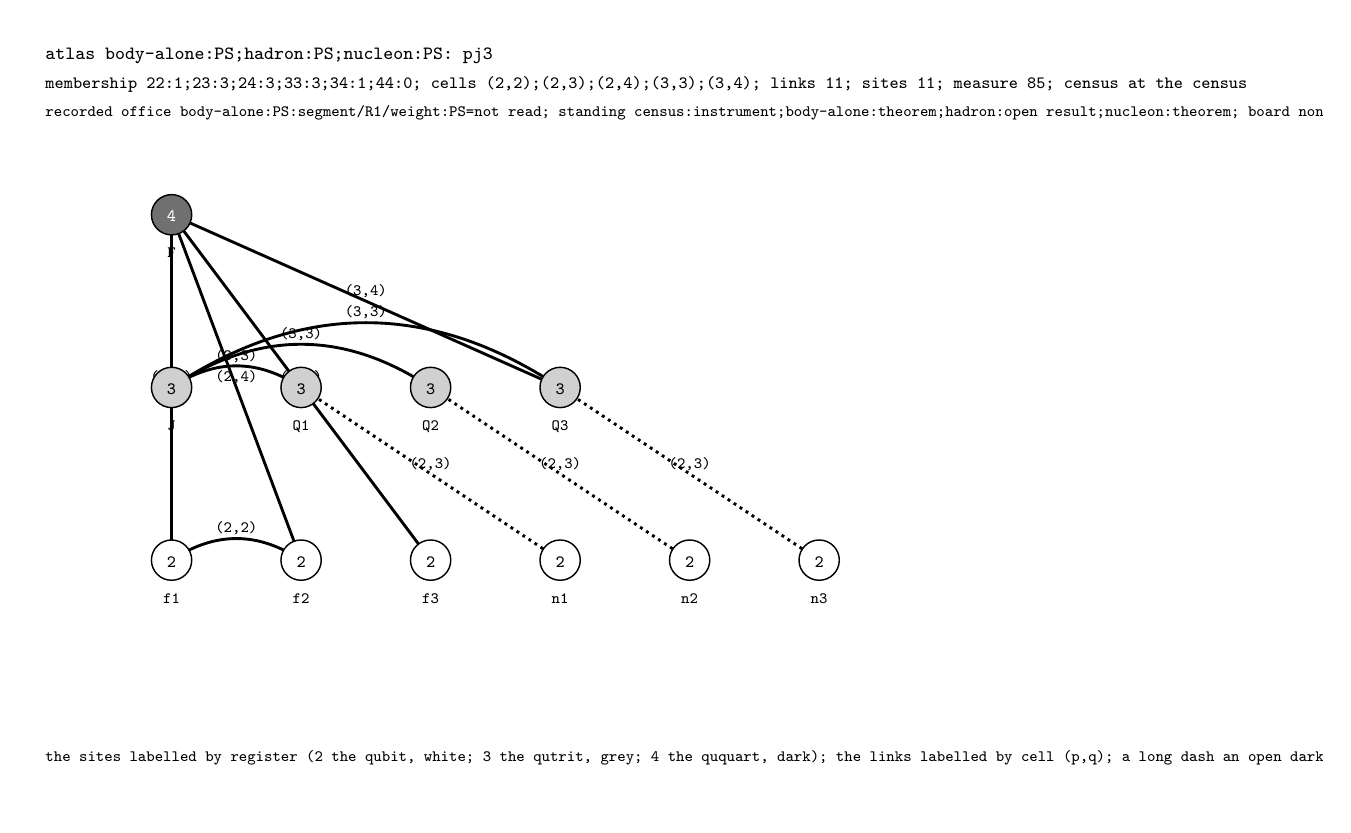
\begin{tikzpicture}[x=0.52pt,y=-0.52pt,baseline]
\clip (0,0) rectangle (900,540);
\fill[white] (0,0) rectangle (900,540);
\node[anchor=base west,inner sep=0pt,text=black,font=\fontsize{6.76}{8.112}\selectfont\ttfamily] at (12,22) {atlas body-alone:PS;hadron:PS;nucleon:PS: pj3};
\node[anchor=base west,inner sep=0pt,text=black,font=\fontsize{6.24}{7.488}\selectfont\ttfamily] at (12,42) {membership 22:1;23:3;24:3;33:3;34:1;44:0; cells (2,2);(2,3);(2,4);(3,3);(3,4); links 11; sites 11; measure 85; census at the census};
\node[anchor=base west,inner sep=0pt,text=black,font=\fontsize{5.72}{6.864}\selectfont\ttfamily] at (12,62) {recorded office body-alone:PS:segment/R1/weight:PS=not read; standing census:instrument;body-alone:theorem;hadron:open result;nucleon:theorem; board none};
\draw[draw=black,line width=1.04pt] (100,130) -- (370,250);
\node[anchor=base,inner sep=0pt,text=black,font=\fontsize{5.72}{6.864}\selectfont\ttfamily] at (235,186) {(3,4)};
\draw[draw=black,line width=1.04pt] (100,130) -- (100,370);
\node[anchor=base,inner sep=0pt,text=black,font=\fontsize{5.72}{6.864}\selectfont\ttfamily] at (100,246) {(2,4)};
\draw[draw=black,line width=1.04pt] (100,130) -- (190,370);
\node[anchor=base,inner sep=0pt,text=black,font=\fontsize{5.72}{6.864}\selectfont\ttfamily] at (145,246) {(2,4)};
\draw[draw=black,line width=1.04pt] (100,130) -- (280,370);
\node[anchor=base,inner sep=0pt,text=black,font=\fontsize{5.72}{6.864}\selectfont\ttfamily] at (190,246) {(2,4)};
\draw[draw=black,line width=1.04pt] (100,250) .. controls (130,230) and (160,230) .. (190,250);
\node[anchor=base,inner sep=0pt,text=black,font=\fontsize{5.72}{6.864}\selectfont\ttfamily] at (145,231) {(3,3)};
\draw[draw=black,line width=1.04pt] (100,250) .. controls (160,210) and (220,210) .. (280,250);
\node[anchor=base,inner sep=0pt,text=black,font=\fontsize{5.72}{6.864}\selectfont\ttfamily] at (190,216) {(3,3)};
\draw[draw=black,line width=1.04pt] (100,250) .. controls (190,190) and (280,190) .. (370,250);
\node[anchor=base,inner sep=0pt,text=black,font=\fontsize{5.72}{6.864}\selectfont\ttfamily] at (235,201) {(3,3)};
\draw[draw=black,line width=1.04pt,dash pattern=on 1.04pt off 1.56pt] (190,250) -- (370,370);
\node[anchor=base,inner sep=0pt,text=black,font=\fontsize{5.72}{6.864}\selectfont\ttfamily] at (280,306) {(2,3)};
\draw[draw=black,line width=1.04pt,dash pattern=on 1.04pt off 1.56pt] (280,250) -- (460,370);
\node[anchor=base,inner sep=0pt,text=black,font=\fontsize{5.72}{6.864}\selectfont\ttfamily] at (370,306) {(2,3)};
\draw[draw=black,line width=1.04pt,dash pattern=on 1.04pt off 1.56pt] (370,250) -- (550,370);
\node[anchor=base,inner sep=0pt,text=black,font=\fontsize{5.72}{6.864}\selectfont\ttfamily] at (460,306) {(2,3)};
\draw[draw=black,line width=1.04pt] (100,370) .. controls (130,350) and (160,350) .. (190,370);
\node[anchor=base,inner sep=0pt,text=black,font=\fontsize{5.72}{6.864}\selectfont\ttfamily] at (145,351) {(2,2)};
\filldraw[fill={rgb,255:red,112;green,112;blue,112},draw=black,line width=0.52pt] (100,130) circle (14);
\node[anchor=base,inner sep=0pt,text=white,font=\fontsize{6.24}{7.488}\selectfont\ttfamily] at (100,135) {4};
\node[anchor=base,inner sep=0pt,text=black,font=\fontsize{5.72}{6.864}\selectfont\ttfamily] at (100,160) {F};
\filldraw[fill={rgb,255:red,208;green,208;blue,208},draw=black,line width=0.52pt] (100,250) circle (14);
\node[anchor=base,inner sep=0pt,text=black,font=\fontsize{6.24}{7.488}\selectfont\ttfamily] at (100,255) {3};
\node[anchor=base,inner sep=0pt,text=black,font=\fontsize{5.72}{6.864}\selectfont\ttfamily] at (100,280) {J};
\filldraw[fill={rgb,255:red,208;green,208;blue,208},draw=black,line width=0.52pt] (190,250) circle (14);
\node[anchor=base,inner sep=0pt,text=black,font=\fontsize{6.24}{7.488}\selectfont\ttfamily] at (190,255) {3};
\node[anchor=base,inner sep=0pt,text=black,font=\fontsize{5.72}{6.864}\selectfont\ttfamily] at (190,280) {Q1};
\filldraw[fill={rgb,255:red,208;green,208;blue,208},draw=black,line width=0.52pt] (280,250) circle (14);
\node[anchor=base,inner sep=0pt,text=black,font=\fontsize{6.24}{7.488}\selectfont\ttfamily] at (280,255) {3};
\node[anchor=base,inner sep=0pt,text=black,font=\fontsize{5.72}{6.864}\selectfont\ttfamily] at (280,280) {Q2};
\filldraw[fill={rgb,255:red,208;green,208;blue,208},draw=black,line width=0.52pt] (370,250) circle (14);
\node[anchor=base,inner sep=0pt,text=black,font=\fontsize{6.24}{7.488}\selectfont\ttfamily] at (370,255) {3};
\node[anchor=base,inner sep=0pt,text=black,font=\fontsize{5.72}{6.864}\selectfont\ttfamily] at (370,280) {Q3};
\filldraw[fill=white,draw=black,line width=0.52pt] (100,370) circle (14);
\node[anchor=base,inner sep=0pt,text=black,font=\fontsize{6.24}{7.488}\selectfont\ttfamily] at (100,375) {2};
\node[anchor=base,inner sep=0pt,text=black,font=\fontsize{5.72}{6.864}\selectfont\ttfamily] at (100,400) {f1};
\filldraw[fill=white,draw=black,line width=0.52pt] (190,370) circle (14);
\node[anchor=base,inner sep=0pt,text=black,font=\fontsize{6.24}{7.488}\selectfont\ttfamily] at (190,375) {2};
\node[anchor=base,inner sep=0pt,text=black,font=\fontsize{5.72}{6.864}\selectfont\ttfamily] at (190,400) {f2};
\filldraw[fill=white,draw=black,line width=0.52pt] (280,370) circle (14);
\node[anchor=base,inner sep=0pt,text=black,font=\fontsize{6.24}{7.488}\selectfont\ttfamily] at (280,375) {2};
\node[anchor=base,inner sep=0pt,text=black,font=\fontsize{5.72}{6.864}\selectfont\ttfamily] at (280,400) {f3};
\filldraw[fill=white,draw=black,line width=0.52pt] (370,370) circle (14);
\node[anchor=base,inner sep=0pt,text=black,font=\fontsize{6.24}{7.488}\selectfont\ttfamily] at (370,375) {2};
\node[anchor=base,inner sep=0pt,text=black,font=\fontsize{5.72}{6.864}\selectfont\ttfamily] at (370,400) {n1};
\filldraw[fill=white,draw=black,line width=0.52pt] (460,370) circle (14);
\node[anchor=base,inner sep=0pt,text=black,font=\fontsize{6.24}{7.488}\selectfont\ttfamily] at (460,375) {2};
\node[anchor=base,inner sep=0pt,text=black,font=\fontsize{5.72}{6.864}\selectfont\ttfamily] at (460,400) {n2};
\filldraw[fill=white,draw=black,line width=0.52pt] (550,370) circle (14);
\node[anchor=base,inner sep=0pt,text=black,font=\fontsize{6.24}{7.488}\selectfont\ttfamily] at (550,375) {2};
\node[anchor=base,inner sep=0pt,text=black,font=\fontsize{5.72}{6.864}\selectfont\ttfamily] at (550,400) {n3};
\node[anchor=base west,inner sep=0pt,text=black,font=\fontsize{5.72}{6.864}\selectfont\ttfamily] at (12,510) {the sites labelled by register (2 the qubit, white; 3 the qutrit, grey; 4 the ququart, dark); the links labelled by cell (p,q); a long dash an open dark link of the neutron row; a short dash a docked link at the rule R1};
\end{tikzpicture}
\caption{\texttt{pj3}, hadron row body, junction star, star: 11 sites, 11 links, the measure 85; the links at the cells (2,2), (2,3), (2,4), (3,3), (3,4); the membership 22:1; 23:3; 24:3; 33:3; 34:1; 44:0; 3 docked links at the rule R1 (Q1-n1; Q2-n2; Q3-n3); at the census of the six cells. Drawn at the anatomy atlas as its web, the sites labeled by register and the links by cell, from the the body-alone office rule.}\label{fig:VIII-2-D537322-pj3-3a81f7}
\begin{center}\footnotesize\begin{adjustbox}{max width=\linewidth}\begin{tabular}{p{0.26\textwidth}p{0.68\textwidth}}\toprule
recorded office (the slot-count row) & the read d-ps of the hadron offices row: the first power 85; the office \texttt{7225\textbar{}0\textbar{}0\textbar{}0}; against the formula with the slot count parts; the slot total 0; dark links 8; hubs F; dressing 3 \\
mass register (the mass-register row) & the read bps: the class touching the ququart; the first power 201; the office \texttt{2 144 666 856 770 839/53084160000\textbar{}661/4050\textbar{}5977541/2654208000\textbar{}0}; nonzero; met yes; hubs F; in-legs Q3-F; dressing 3; ports Q1-n1; Q2-n2; Q3-n3; F-f3 \\
junction registers (the hadron row) & the read PS: junctions J; Q3; the share one third per leg; the registers at the share 85, struck 67, mono 255, the hub spelling 255; against the cells 85; 67; 255; 3, equal \\
\bottomrule\end{tabular}\end{adjustbox}\end{center}
\end{figure}
\begin{figure}[H]\centering
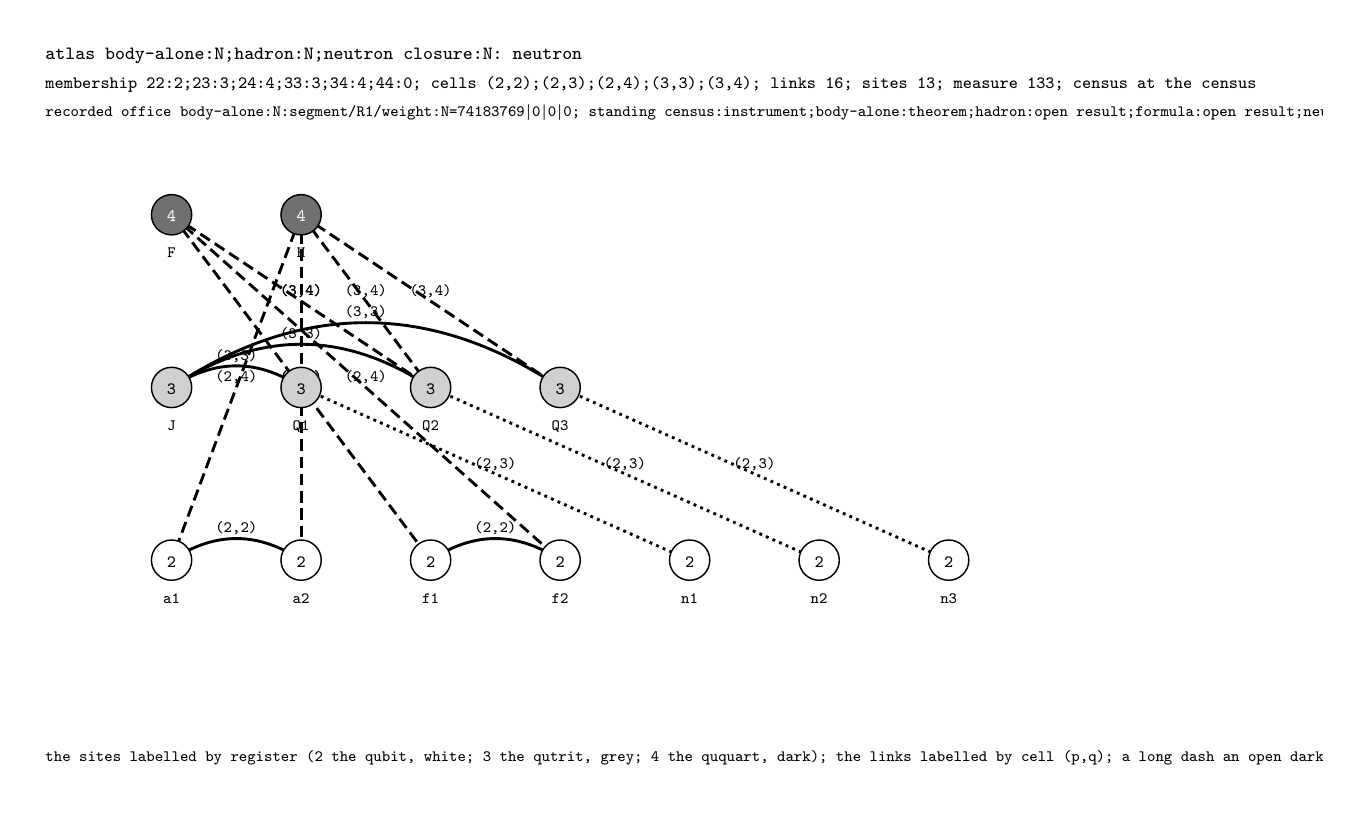
\begin{tikzpicture}[x=0.52pt,y=-0.52pt,baseline]
\clip (0,0) rectangle (900,540);
\fill[white] (0,0) rectangle (900,540);
\node[anchor=base west,inner sep=0pt,text=black,font=\fontsize{6.76}{8.112}\selectfont\ttfamily] at (12,22) {atlas body-alone:N;hadron:N;neutron closure:N: neutron};
\node[anchor=base west,inner sep=0pt,text=black,font=\fontsize{6.24}{7.488}\selectfont\ttfamily] at (12,42) {membership 22:2;23:3;24:4;33:3;34:4;44:0; cells (2,2);(2,3);(2,4);(3,3);(3,4); links 16; sites 13; measure 133; census at the census};
\node[anchor=base west,inner sep=0pt,text=black,font=\fontsize{5.72}{6.864}\selectfont\ttfamily] at (12,62) {recorded office body-alone:N:segment/R1/weight:N=74183769\textbar{}0\textbar{}0\textbar{}0; standing census:instrument;body-alone:theorem;hadron:open result;formula:open result;neutron closure:open result; board proton};
\draw[draw=black,line width=1.04pt,dash pattern=on 4.16pt off 2.08pt] (100,130) -- (280,250);
\node[anchor=base,inner sep=0pt,text=black,font=\fontsize{5.72}{6.864}\selectfont\ttfamily] at (190,186) {(3,4)};
\draw[draw=black,line width=1.04pt,dash pattern=on 4.16pt off 2.08pt] (100,130) -- (280,370);
\node[anchor=base,inner sep=0pt,text=black,font=\fontsize{5.72}{6.864}\selectfont\ttfamily] at (190,246) {(2,4)};
\draw[draw=black,line width=1.04pt,dash pattern=on 4.16pt off 2.08pt] (100,130) -- (370,370);
\node[anchor=base,inner sep=0pt,text=black,font=\fontsize{5.72}{6.864}\selectfont\ttfamily] at (235,246) {(2,4)};
\draw[draw=black,line width=1.04pt,dash pattern=on 4.16pt off 2.08pt] (190,130) -- (190,250);
\node[anchor=base,inner sep=0pt,text=black,font=\fontsize{5.72}{6.864}\selectfont\ttfamily] at (190,186) {(3,4)};
\draw[draw=black,line width=1.04pt,dash pattern=on 4.16pt off 2.08pt] (190,130) -- (280,250);
\node[anchor=base,inner sep=0pt,text=black,font=\fontsize{5.72}{6.864}\selectfont\ttfamily] at (235,186) {(3,4)};
\draw[draw=black,line width=1.04pt,dash pattern=on 4.16pt off 2.08pt] (190,130) -- (370,250);
\node[anchor=base,inner sep=0pt,text=black,font=\fontsize{5.72}{6.864}\selectfont\ttfamily] at (280,186) {(3,4)};
\draw[draw=black,line width=1.04pt,dash pattern=on 4.16pt off 2.08pt] (190,130) -- (100,370);
\node[anchor=base,inner sep=0pt,text=black,font=\fontsize{5.72}{6.864}\selectfont\ttfamily] at (145,246) {(2,4)};
\draw[draw=black,line width=1.04pt,dash pattern=on 4.16pt off 2.08pt] (190,130) -- (190,370);
\node[anchor=base,inner sep=0pt,text=black,font=\fontsize{5.72}{6.864}\selectfont\ttfamily] at (190,246) {(2,4)};
\draw[draw=black,line width=1.04pt] (100,250) .. controls (130,230) and (160,230) .. (190,250);
\node[anchor=base,inner sep=0pt,text=black,font=\fontsize{5.72}{6.864}\selectfont\ttfamily] at (145,231) {(3,3)};
\draw[draw=black,line width=1.04pt] (100,250) .. controls (160,210) and (220,210) .. (280,250);
\node[anchor=base,inner sep=0pt,text=black,font=\fontsize{5.72}{6.864}\selectfont\ttfamily] at (190,216) {(3,3)};
\draw[draw=black,line width=1.04pt] (100,250) .. controls (190,190) and (280,190) .. (370,250);
\node[anchor=base,inner sep=0pt,text=black,font=\fontsize{5.72}{6.864}\selectfont\ttfamily] at (235,201) {(3,3)};
\draw[draw=black,line width=1.04pt,dash pattern=on 1.04pt off 1.56pt] (190,250) -- (460,370);
\node[anchor=base,inner sep=0pt,text=black,font=\fontsize{5.72}{6.864}\selectfont\ttfamily] at (325,306) {(2,3)};
\draw[draw=black,line width=1.04pt,dash pattern=on 1.04pt off 1.56pt] (280,250) -- (550,370);
\node[anchor=base,inner sep=0pt,text=black,font=\fontsize{5.72}{6.864}\selectfont\ttfamily] at (415,306) {(2,3)};
\draw[draw=black,line width=1.04pt,dash pattern=on 1.04pt off 1.56pt] (370,250) -- (640,370);
\node[anchor=base,inner sep=0pt,text=black,font=\fontsize{5.72}{6.864}\selectfont\ttfamily] at (505,306) {(2,3)};
\draw[draw=black,line width=1.04pt] (100,370) .. controls (130,350) and (160,350) .. (190,370);
\node[anchor=base,inner sep=0pt,text=black,font=\fontsize{5.72}{6.864}\selectfont\ttfamily] at (145,351) {(2,2)};
\draw[draw=black,line width=1.04pt] (280,370) .. controls (310,350) and (340,350) .. (370,370);
\node[anchor=base,inner sep=0pt,text=black,font=\fontsize{5.72}{6.864}\selectfont\ttfamily] at (325,351) {(2,2)};
\filldraw[fill={rgb,255:red,112;green,112;blue,112},draw=black,line width=0.52pt] (100,130) circle (14);
\node[anchor=base,inner sep=0pt,text=white,font=\fontsize{6.24}{7.488}\selectfont\ttfamily] at (100,135) {4};
\node[anchor=base,inner sep=0pt,text=black,font=\fontsize{5.72}{6.864}\selectfont\ttfamily] at (100,160) {F};
\filldraw[fill={rgb,255:red,112;green,112;blue,112},draw=black,line width=0.52pt] (190,130) circle (14);
\node[anchor=base,inner sep=0pt,text=white,font=\fontsize{6.24}{7.488}\selectfont\ttfamily] at (190,135) {4};
\node[anchor=base,inner sep=0pt,text=black,font=\fontsize{5.72}{6.864}\selectfont\ttfamily] at (190,160) {H};
\filldraw[fill={rgb,255:red,208;green,208;blue,208},draw=black,line width=0.52pt] (100,250) circle (14);
\node[anchor=base,inner sep=0pt,text=black,font=\fontsize{6.24}{7.488}\selectfont\ttfamily] at (100,255) {3};
\node[anchor=base,inner sep=0pt,text=black,font=\fontsize{5.72}{6.864}\selectfont\ttfamily] at (100,280) {J};
\filldraw[fill={rgb,255:red,208;green,208;blue,208},draw=black,line width=0.52pt] (190,250) circle (14);
\node[anchor=base,inner sep=0pt,text=black,font=\fontsize{6.24}{7.488}\selectfont\ttfamily] at (190,255) {3};
\node[anchor=base,inner sep=0pt,text=black,font=\fontsize{5.72}{6.864}\selectfont\ttfamily] at (190,280) {Q1};
\filldraw[fill={rgb,255:red,208;green,208;blue,208},draw=black,line width=0.52pt] (280,250) circle (14);
\node[anchor=base,inner sep=0pt,text=black,font=\fontsize{6.24}{7.488}\selectfont\ttfamily] at (280,255) {3};
\node[anchor=base,inner sep=0pt,text=black,font=\fontsize{5.72}{6.864}\selectfont\ttfamily] at (280,280) {Q2};
\filldraw[fill={rgb,255:red,208;green,208;blue,208},draw=black,line width=0.52pt] (370,250) circle (14);
\node[anchor=base,inner sep=0pt,text=black,font=\fontsize{6.24}{7.488}\selectfont\ttfamily] at (370,255) {3};
\node[anchor=base,inner sep=0pt,text=black,font=\fontsize{5.72}{6.864}\selectfont\ttfamily] at (370,280) {Q3};
\filldraw[fill=white,draw=black,line width=0.52pt] (100,370) circle (14);
\node[anchor=base,inner sep=0pt,text=black,font=\fontsize{6.24}{7.488}\selectfont\ttfamily] at (100,375) {2};
\node[anchor=base,inner sep=0pt,text=black,font=\fontsize{5.72}{6.864}\selectfont\ttfamily] at (100,400) {a1};
\filldraw[fill=white,draw=black,line width=0.52pt] (190,370) circle (14);
\node[anchor=base,inner sep=0pt,text=black,font=\fontsize{6.24}{7.488}\selectfont\ttfamily] at (190,375) {2};
\node[anchor=base,inner sep=0pt,text=black,font=\fontsize{5.72}{6.864}\selectfont\ttfamily] at (190,400) {a2};
\filldraw[fill=white,draw=black,line width=0.52pt] (280,370) circle (14);
\node[anchor=base,inner sep=0pt,text=black,font=\fontsize{6.24}{7.488}\selectfont\ttfamily] at (280,375) {2};
\node[anchor=base,inner sep=0pt,text=black,font=\fontsize{5.72}{6.864}\selectfont\ttfamily] at (280,400) {f1};
\filldraw[fill=white,draw=black,line width=0.52pt] (370,370) circle (14);
\node[anchor=base,inner sep=0pt,text=black,font=\fontsize{6.24}{7.488}\selectfont\ttfamily] at (370,375) {2};
\node[anchor=base,inner sep=0pt,text=black,font=\fontsize{5.72}{6.864}\selectfont\ttfamily] at (370,400) {f2};
\filldraw[fill=white,draw=black,line width=0.52pt] (460,370) circle (14);
\node[anchor=base,inner sep=0pt,text=black,font=\fontsize{6.24}{7.488}\selectfont\ttfamily] at (460,375) {2};
\node[anchor=base,inner sep=0pt,text=black,font=\fontsize{5.72}{6.864}\selectfont\ttfamily] at (460,400) {n1};
\filldraw[fill=white,draw=black,line width=0.52pt] (550,370) circle (14);
\node[anchor=base,inner sep=0pt,text=black,font=\fontsize{6.24}{7.488}\selectfont\ttfamily] at (550,375) {2};
\node[anchor=base,inner sep=0pt,text=black,font=\fontsize{5.72}{6.864}\selectfont\ttfamily] at (550,400) {n2};
\filldraw[fill=white,draw=black,line width=0.52pt] (640,370) circle (14);
\node[anchor=base,inner sep=0pt,text=black,font=\fontsize{6.24}{7.488}\selectfont\ttfamily] at (640,375) {2};
\node[anchor=base,inner sep=0pt,text=black,font=\fontsize{5.72}{6.864}\selectfont\ttfamily] at (640,400) {n3};
\node[anchor=base west,inner sep=0pt,text=black,font=\fontsize{5.72}{6.864}\selectfont\ttfamily] at (12,510) {the sites labelled by register (2 the qubit, white; 3 the qutrit, grey; 4 the ququart, dark); the links labelled by cell (p,q); a long dash an open dark link of the neutron row; a short dash a docked link at the rule R1};
\end{tikzpicture}
\caption{\texttt{neutron} (the proton), recorded body, hadron row body, neutron at its own typing: 13 sites, 16 links, the measure 133; the links at the cells (2,2), (2,3), (2,4), (3,3), (3,4); the membership 22:2; 23:3; 24:4; 33:3; 34:4; 44:0; 3 docked links at the rule R1 (Q1-n1; Q2-n2; Q3-n3); 8 open dark links of the neutron row; at the census of the six cells. Drawn at the anatomy atlas as its web, the sites labeled by register and the links by cell, from the the body-alone office rule.}\label{fig:VIII-2-D537322-neutron-9be5ea}
\begin{center}\footnotesize\begin{adjustbox}{max width=\linewidth}\begin{tabular}{p{0.26\textwidth}p{0.68\textwidth}}\toprule
recorded office (the slot-count row) & the read o-n of the formula row: the first power 8613; the office \texttt{74183769\textbar{}0\textbar{}0\textbar{}0}; against the formula with the slot count equal; the slot total 1; dark links 13; hubs H; F; dressing 27 \\
mass register (the mass-register row) & the read BN: the class touching the ququart; the first power 9315; the office \texttt{56 865 317 258 729 151/655360000\textbar{}5841/25\textbar{}320665041/163840000\textbar{}0}; nonzero; met yes; hubs F; H; in-legs H-Q1; H-Q2; H-Q3; Q2-F; dressing 81; ports Q1-n1; Q2-n2; Q3-n3 \\
junction registers (the hadron row) & the read N: junctions J; Q1; Q3; the share one third per leg; the registers at the share 133, struck 115, mono 1596, the hub spelling 3591; against the cells none; none; none; none, none \\
\bottomrule\end{tabular}\end{adjustbox}\end{center}
\end{figure}
\begin{figure}[H]\centering
\begin{adjustbox}{max width=\linewidth}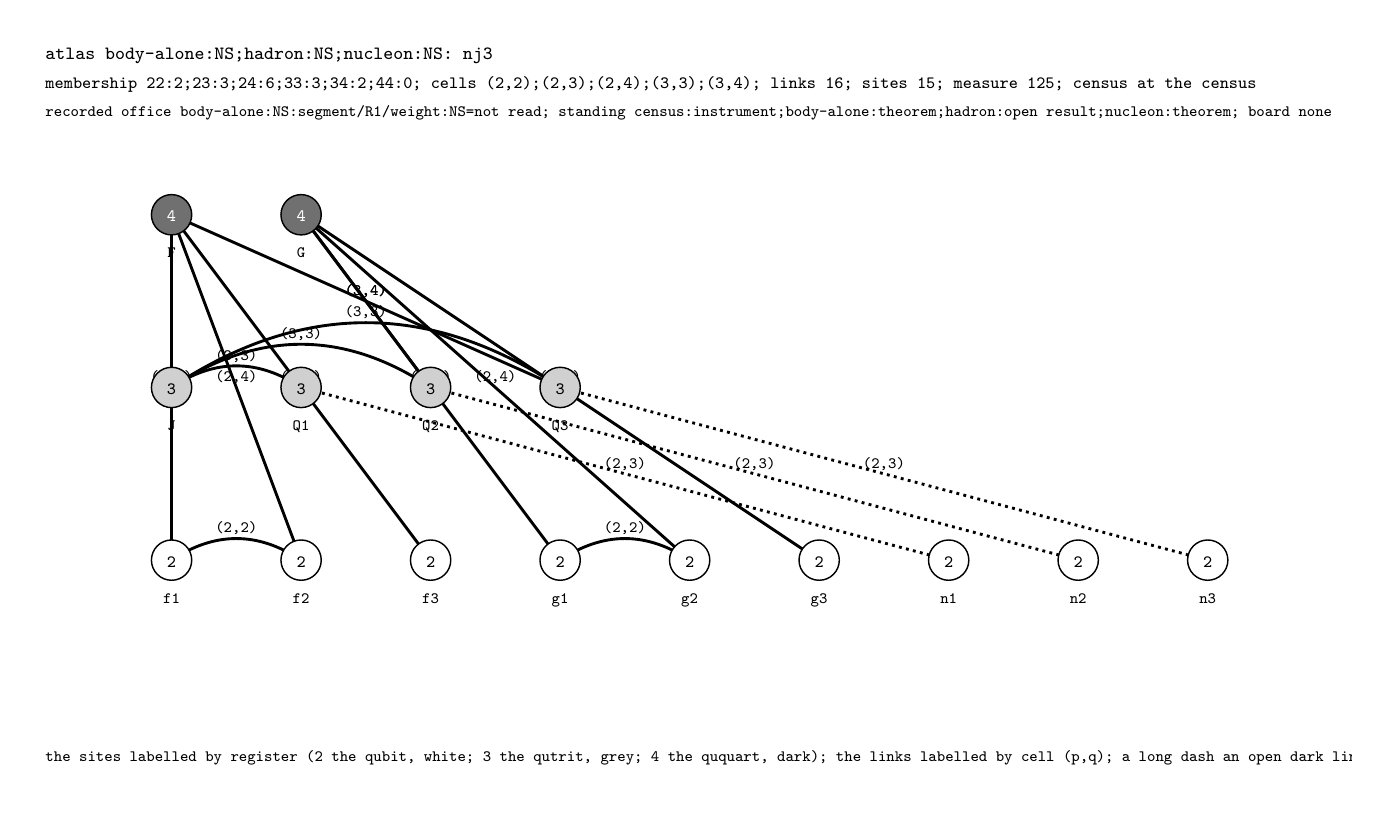
\begin{tikzpicture}[x=0.52pt,y=-0.52pt,baseline]
\clip (0,0) rectangle (920,540);
\fill[white] (0,0) rectangle (920,540);
\node[anchor=base west,inner sep=0pt,text=black,font=\fontsize{6.76}{8.112}\selectfont\ttfamily] at (12,22) {atlas body-alone:NS;hadron:NS;nucleon:NS: nj3};
\node[anchor=base west,inner sep=0pt,text=black,font=\fontsize{6.24}{7.488}\selectfont\ttfamily] at (12,42) {membership 22:2;23:3;24:6;33:3;34:2;44:0; cells (2,2);(2,3);(2,4);(3,3);(3,4); links 16; sites 15; measure 125; census at the census};
\node[anchor=base west,inner sep=0pt,text=black,font=\fontsize{5.72}{6.864}\selectfont\ttfamily] at (12,62) {recorded office body-alone:NS:segment/R1/weight:NS=not read; standing census:instrument;body-alone:theorem;hadron:open result;nucleon:theorem; board none};
\draw[draw=black,line width=1.04pt] (100,130) -- (370,250);
\node[anchor=base,inner sep=0pt,text=black,font=\fontsize{5.72}{6.864}\selectfont\ttfamily] at (235,186) {(3,4)};
\draw[draw=black,line width=1.04pt] (100,130) -- (100,370);
\node[anchor=base,inner sep=0pt,text=black,font=\fontsize{5.72}{6.864}\selectfont\ttfamily] at (100,246) {(2,4)};
\draw[draw=black,line width=1.04pt] (100,130) -- (190,370);
\node[anchor=base,inner sep=0pt,text=black,font=\fontsize{5.72}{6.864}\selectfont\ttfamily] at (145,246) {(2,4)};
\draw[draw=black,line width=1.04pt] (100,130) -- (280,370);
\node[anchor=base,inner sep=0pt,text=black,font=\fontsize{5.72}{6.864}\selectfont\ttfamily] at (190,246) {(2,4)};
\draw[draw=black,line width=1.04pt] (190,130) -- (280,250);
\node[anchor=base,inner sep=0pt,text=black,font=\fontsize{5.72}{6.864}\selectfont\ttfamily] at (235,186) {(3,4)};
\draw[draw=black,line width=1.04pt] (190,130) -- (370,370);
\node[anchor=base,inner sep=0pt,text=black,font=\fontsize{5.72}{6.864}\selectfont\ttfamily] at (280,246) {(2,4)};
\draw[draw=black,line width=1.04pt] (190,130) -- (460,370);
\node[anchor=base,inner sep=0pt,text=black,font=\fontsize{5.72}{6.864}\selectfont\ttfamily] at (325,246) {(2,4)};
\draw[draw=black,line width=1.04pt] (190,130) -- (550,370);
\node[anchor=base,inner sep=0pt,text=black,font=\fontsize{5.72}{6.864}\selectfont\ttfamily] at (370,246) {(2,4)};
\draw[draw=black,line width=1.04pt] (100,250) .. controls (130,230) and (160,230) .. (190,250);
\node[anchor=base,inner sep=0pt,text=black,font=\fontsize{5.72}{6.864}\selectfont\ttfamily] at (145,231) {(3,3)};
\draw[draw=black,line width=1.04pt] (100,250) .. controls (160,210) and (220,210) .. (280,250);
\node[anchor=base,inner sep=0pt,text=black,font=\fontsize{5.72}{6.864}\selectfont\ttfamily] at (190,216) {(3,3)};
\draw[draw=black,line width=1.04pt] (100,250) .. controls (190,190) and (280,190) .. (370,250);
\node[anchor=base,inner sep=0pt,text=black,font=\fontsize{5.72}{6.864}\selectfont\ttfamily] at (235,201) {(3,3)};
\draw[draw=black,line width=1.04pt,dash pattern=on 1.04pt off 1.56pt] (190,250) -- (640,370);
\node[anchor=base,inner sep=0pt,text=black,font=\fontsize{5.72}{6.864}\selectfont\ttfamily] at (415,306) {(2,3)};
\draw[draw=black,line width=1.04pt,dash pattern=on 1.04pt off 1.56pt] (280,250) -- (730,370);
\node[anchor=base,inner sep=0pt,text=black,font=\fontsize{5.72}{6.864}\selectfont\ttfamily] at (505,306) {(2,3)};
\draw[draw=black,line width=1.04pt,dash pattern=on 1.04pt off 1.56pt] (370,250) -- (820,370);
\node[anchor=base,inner sep=0pt,text=black,font=\fontsize{5.72}{6.864}\selectfont\ttfamily] at (595,306) {(2,3)};
\draw[draw=black,line width=1.04pt] (100,370) .. controls (130,350) and (160,350) .. (190,370);
\node[anchor=base,inner sep=0pt,text=black,font=\fontsize{5.72}{6.864}\selectfont\ttfamily] at (145,351) {(2,2)};
\draw[draw=black,line width=1.04pt] (370,370) .. controls (400,350) and (430,350) .. (460,370);
\node[anchor=base,inner sep=0pt,text=black,font=\fontsize{5.72}{6.864}\selectfont\ttfamily] at (415,351) {(2,2)};
\filldraw[fill={rgb,255:red,112;green,112;blue,112},draw=black,line width=0.52pt] (100,130) circle (14);
\node[anchor=base,inner sep=0pt,text=white,font=\fontsize{6.24}{7.488}\selectfont\ttfamily] at (100,135) {4};
\node[anchor=base,inner sep=0pt,text=black,font=\fontsize{5.72}{6.864}\selectfont\ttfamily] at (100,160) {F};
\filldraw[fill={rgb,255:red,112;green,112;blue,112},draw=black,line width=0.52pt] (190,130) circle (14);
\node[anchor=base,inner sep=0pt,text=white,font=\fontsize{6.24}{7.488}\selectfont\ttfamily] at (190,135) {4};
\node[anchor=base,inner sep=0pt,text=black,font=\fontsize{5.72}{6.864}\selectfont\ttfamily] at (190,160) {G};
\filldraw[fill={rgb,255:red,208;green,208;blue,208},draw=black,line width=0.52pt] (100,250) circle (14);
\node[anchor=base,inner sep=0pt,text=black,font=\fontsize{6.24}{7.488}\selectfont\ttfamily] at (100,255) {3};
\node[anchor=base,inner sep=0pt,text=black,font=\fontsize{5.72}{6.864}\selectfont\ttfamily] at (100,280) {J};
\filldraw[fill={rgb,255:red,208;green,208;blue,208},draw=black,line width=0.52pt] (190,250) circle (14);
\node[anchor=base,inner sep=0pt,text=black,font=\fontsize{6.24}{7.488}\selectfont\ttfamily] at (190,255) {3};
\node[anchor=base,inner sep=0pt,text=black,font=\fontsize{5.72}{6.864}\selectfont\ttfamily] at (190,280) {Q1};
\filldraw[fill={rgb,255:red,208;green,208;blue,208},draw=black,line width=0.52pt] (280,250) circle (14);
\node[anchor=base,inner sep=0pt,text=black,font=\fontsize{6.24}{7.488}\selectfont\ttfamily] at (280,255) {3};
\node[anchor=base,inner sep=0pt,text=black,font=\fontsize{5.72}{6.864}\selectfont\ttfamily] at (280,280) {Q2};
\filldraw[fill={rgb,255:red,208;green,208;blue,208},draw=black,line width=0.52pt] (370,250) circle (14);
\node[anchor=base,inner sep=0pt,text=black,font=\fontsize{6.24}{7.488}\selectfont\ttfamily] at (370,255) {3};
\node[anchor=base,inner sep=0pt,text=black,font=\fontsize{5.72}{6.864}\selectfont\ttfamily] at (370,280) {Q3};
\filldraw[fill=white,draw=black,line width=0.52pt] (100,370) circle (14);
\node[anchor=base,inner sep=0pt,text=black,font=\fontsize{6.24}{7.488}\selectfont\ttfamily] at (100,375) {2};
\node[anchor=base,inner sep=0pt,text=black,font=\fontsize{5.72}{6.864}\selectfont\ttfamily] at (100,400) {f1};
\filldraw[fill=white,draw=black,line width=0.52pt] (190,370) circle (14);
\node[anchor=base,inner sep=0pt,text=black,font=\fontsize{6.24}{7.488}\selectfont\ttfamily] at (190,375) {2};
\node[anchor=base,inner sep=0pt,text=black,font=\fontsize{5.72}{6.864}\selectfont\ttfamily] at (190,400) {f2};
\filldraw[fill=white,draw=black,line width=0.52pt] (280,370) circle (14);
\node[anchor=base,inner sep=0pt,text=black,font=\fontsize{6.24}{7.488}\selectfont\ttfamily] at (280,375) {2};
\node[anchor=base,inner sep=0pt,text=black,font=\fontsize{5.72}{6.864}\selectfont\ttfamily] at (280,400) {f3};
\filldraw[fill=white,draw=black,line width=0.52pt] (370,370) circle (14);
\node[anchor=base,inner sep=0pt,text=black,font=\fontsize{6.24}{7.488}\selectfont\ttfamily] at (370,375) {2};
\node[anchor=base,inner sep=0pt,text=black,font=\fontsize{5.72}{6.864}\selectfont\ttfamily] at (370,400) {g1};
\filldraw[fill=white,draw=black,line width=0.52pt] (460,370) circle (14);
\node[anchor=base,inner sep=0pt,text=black,font=\fontsize{6.24}{7.488}\selectfont\ttfamily] at (460,375) {2};
\node[anchor=base,inner sep=0pt,text=black,font=\fontsize{5.72}{6.864}\selectfont\ttfamily] at (460,400) {g2};
\filldraw[fill=white,draw=black,line width=0.52pt] (550,370) circle (14);
\node[anchor=base,inner sep=0pt,text=black,font=\fontsize{6.24}{7.488}\selectfont\ttfamily] at (550,375) {2};
\node[anchor=base,inner sep=0pt,text=black,font=\fontsize{5.72}{6.864}\selectfont\ttfamily] at (550,400) {g3};
\filldraw[fill=white,draw=black,line width=0.52pt] (640,370) circle (14);
\node[anchor=base,inner sep=0pt,text=black,font=\fontsize{6.24}{7.488}\selectfont\ttfamily] at (640,375) {2};
\node[anchor=base,inner sep=0pt,text=black,font=\fontsize{5.72}{6.864}\selectfont\ttfamily] at (640,400) {n1};
\filldraw[fill=white,draw=black,line width=0.52pt] (730,370) circle (14);
\node[anchor=base,inner sep=0pt,text=black,font=\fontsize{6.24}{7.488}\selectfont\ttfamily] at (730,375) {2};
\node[anchor=base,inner sep=0pt,text=black,font=\fontsize{5.72}{6.864}\selectfont\ttfamily] at (730,400) {n2};
\filldraw[fill=white,draw=black,line width=0.52pt] (820,370) circle (14);
\node[anchor=base,inner sep=0pt,text=black,font=\fontsize{6.24}{7.488}\selectfont\ttfamily] at (820,375) {2};
\node[anchor=base,inner sep=0pt,text=black,font=\fontsize{5.72}{6.864}\selectfont\ttfamily] at (820,400) {n3};
\node[anchor=base west,inner sep=0pt,text=black,font=\fontsize{5.72}{6.864}\selectfont\ttfamily] at (12,510) {the sites labelled by register (2 the qubit, white; 3 the qutrit, grey; 4 the ququart, dark); the links labelled by cell (p,q); a long dash an open dark link of the neutron row; a short dash a docked link at the rule R1};
\end{tikzpicture}\end{adjustbox}
\caption{\texttt{nj3}, hadron row body, junction star, star: 15 sites, 16 links, the measure 125; the links at the cells (2,2), (2,3), (2,4), (3,3), (3,4); the membership 22:2; 23:3; 24:6; 33:3; 34:2; 44:0; 3 docked links at the rule R1 (Q1-n1; Q2-n2; Q3-n3); at the census of the six cells. Drawn at the anatomy atlas as its web, the sites labeled by register and the links by cell, from the the body-alone office rule.}\label{fig:VIII-2-D537322-nj3-b62b70}
\begin{center}\footnotesize\begin{adjustbox}{max width=\linewidth}\begin{tabular}{p{0.26\textwidth}p{0.68\textwidth}}\toprule
recorded office (the slot-count row) & no read of this body at the slot-count row \\
mass register (the mass-register row) & the read bns: the class touching the ququart; the first power 963; the office \texttt{5 469 872 145 467 303/5898240000\textbar{}661/225\textbar{}6301957/294912000\textbar{}0}; nonzero; met yes; hubs F; G; in-legs Q3-F; Q2-G; dressing 9; ports Q1-n1; Q2-n2; Q3-n3; F-f3; G-g3 \\
junction registers (the hadron row) & the read NS: junctions J; Q2; Q3; the share one third per leg; the registers at the share 125, struck 107, mono 1125, the hub spelling 1125; against the cells 125; 107; 1125; 9, equal \\
\bottomrule\end{tabular}\end{adjustbox}\end{center}
\end{figure}
\begin{figure}[H]\centering
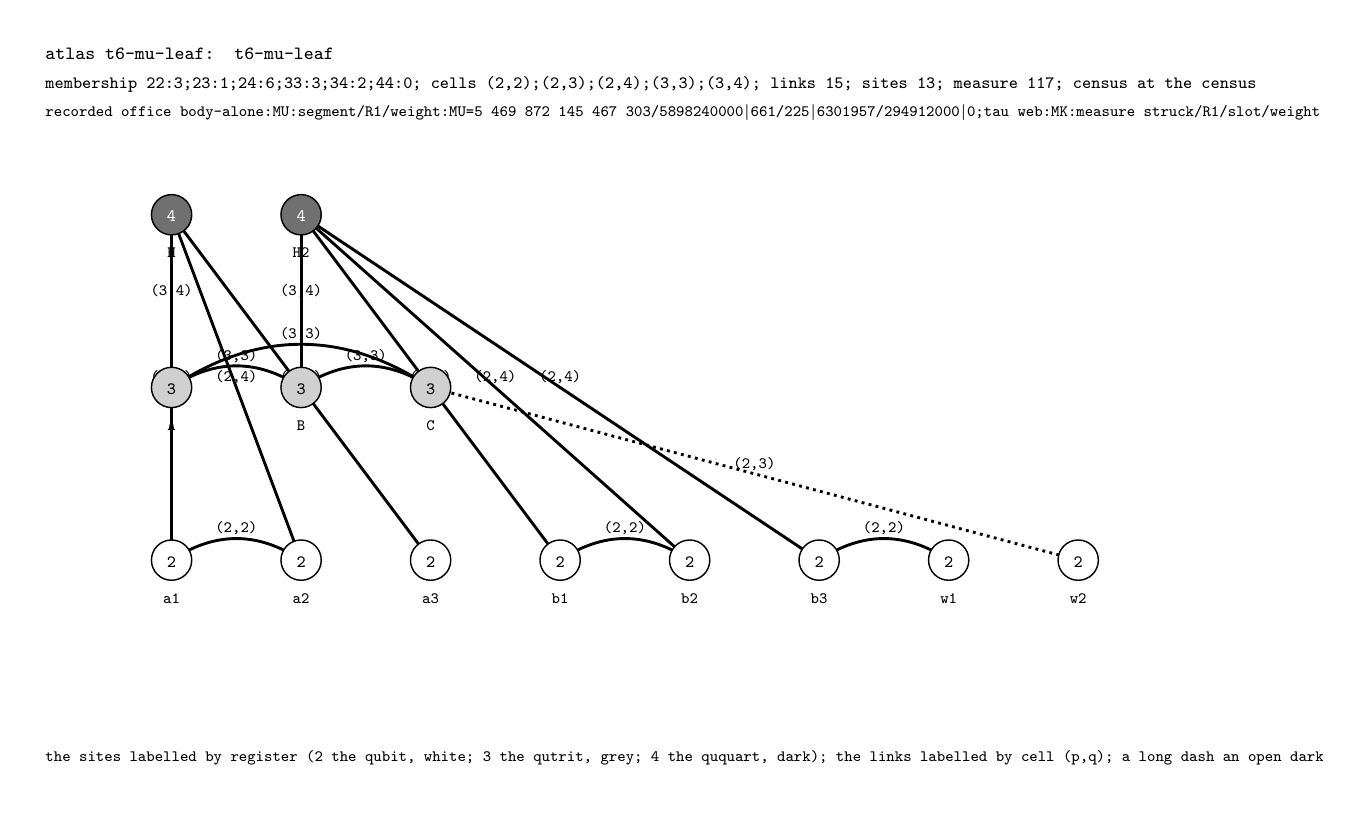
\begin{tikzpicture}[x=0.52pt,y=-0.52pt,baseline]
\clip (0,0) rectangle (900,540);
\fill[white] (0,0) rectangle (900,540);
\node[anchor=base west,inner sep=0pt,text=black,font=\fontsize{6.76}{8.112}\selectfont\ttfamily] at (12,22) {atlas t6-mu-leaf: t6-mu-leaf};
\node[anchor=base west,inner sep=0pt,text=black,font=\fontsize{6.24}{7.488}\selectfont\ttfamily] at (12,42) {membership 22:3;23:1;24:6;33:3;34:2;44:0; cells (2,2);(2,3);(2,4);(3,3);(3,4); links 15; sites 13; measure 117; census at the census};
\node[anchor=base west,inner sep=0pt,text=black,font=\fontsize{5.72}{6.864}\selectfont\ttfamily] at (12,62) {recorded office body-alone:MU:segment/R1/weight:MU=5 469 872 145 467 303/5898240000\textbar{}661/225\textbar{}6301957/294912000\textbar{}0;tau web:MK:measure struck/R1/slot/weight:MK=5 469 872 145 467 303/5898240000\textbar{}661/225\textbar{}6301957/294912000\textbar{}0; standing census:instrument;body-alone:theorem;formula:open result;tau web:theorem;roster:roster word; board muon};
\draw[draw=black,line width=1.04pt] (100,250) .. controls (130,230) and (160,230) .. (190,250);
\node[anchor=base,inner sep=0pt,text=black,font=\fontsize{5.72}{6.864}\selectfont\ttfamily] at (145,231) {(3,3)};
\draw[draw=black,line width=1.04pt] (100,250) .. controls (160,210) and (220,210) .. (280,250);
\node[anchor=base,inner sep=0pt,text=black,font=\fontsize{5.72}{6.864}\selectfont\ttfamily] at (190,216) {(3,3)};
\draw[draw=black,line width=1.04pt] (100,250) -- (100,130);
\node[anchor=base,inner sep=0pt,text=black,font=\fontsize{5.72}{6.864}\selectfont\ttfamily] at (100,186) {(3,4)};
\draw[draw=black,line width=1.04pt] (190,250) .. controls (220,230) and (250,230) .. (280,250);
\node[anchor=base,inner sep=0pt,text=black,font=\fontsize{5.72}{6.864}\selectfont\ttfamily] at (235,231) {(3,3)};
\draw[draw=black,line width=1.04pt] (190,250) -- (190,130);
\node[anchor=base,inner sep=0pt,text=black,font=\fontsize{5.72}{6.864}\selectfont\ttfamily] at (190,186) {(3,4)};
\draw[draw=black,line width=1.04pt,dash pattern=on 1.04pt off 1.56pt] (280,250) -- (730,370);
\node[anchor=base,inner sep=0pt,text=black,font=\fontsize{5.72}{6.864}\selectfont\ttfamily] at (505,306) {(2,3)};
\draw[draw=black,line width=1.04pt] (100,130) -- (100,370);
\node[anchor=base,inner sep=0pt,text=black,font=\fontsize{5.72}{6.864}\selectfont\ttfamily] at (100,246) {(2,4)};
\draw[draw=black,line width=1.04pt] (100,130) -- (190,370);
\node[anchor=base,inner sep=0pt,text=black,font=\fontsize{5.72}{6.864}\selectfont\ttfamily] at (145,246) {(2,4)};
\draw[draw=black,line width=1.04pt] (100,130) -- (280,370);
\node[anchor=base,inner sep=0pt,text=black,font=\fontsize{5.72}{6.864}\selectfont\ttfamily] at (190,246) {(2,4)};
\draw[draw=black,line width=1.04pt] (190,130) -- (370,370);
\node[anchor=base,inner sep=0pt,text=black,font=\fontsize{5.72}{6.864}\selectfont\ttfamily] at (280,246) {(2,4)};
\draw[draw=black,line width=1.04pt] (190,130) -- (460,370);
\node[anchor=base,inner sep=0pt,text=black,font=\fontsize{5.72}{6.864}\selectfont\ttfamily] at (325,246) {(2,4)};
\draw[draw=black,line width=1.04pt] (190,130) -- (550,370);
\node[anchor=base,inner sep=0pt,text=black,font=\fontsize{5.72}{6.864}\selectfont\ttfamily] at (370,246) {(2,4)};
\draw[draw=black,line width=1.04pt] (100,370) .. controls (130,350) and (160,350) .. (190,370);
\node[anchor=base,inner sep=0pt,text=black,font=\fontsize{5.72}{6.864}\selectfont\ttfamily] at (145,351) {(2,2)};
\draw[draw=black,line width=1.04pt] (370,370) .. controls (400,350) and (430,350) .. (460,370);
\node[anchor=base,inner sep=0pt,text=black,font=\fontsize{5.72}{6.864}\selectfont\ttfamily] at (415,351) {(2,2)};
\draw[draw=black,line width=1.04pt] (550,370) .. controls (580,350) and (610,350) .. (640,370);
\node[anchor=base,inner sep=0pt,text=black,font=\fontsize{5.72}{6.864}\selectfont\ttfamily] at (595,351) {(2,2)};
\filldraw[fill={rgb,255:red,208;green,208;blue,208},draw=black,line width=0.52pt] (100,250) circle (14);
\node[anchor=base,inner sep=0pt,text=black,font=\fontsize{6.24}{7.488}\selectfont\ttfamily] at (100,255) {3};
\node[anchor=base,inner sep=0pt,text=black,font=\fontsize{5.72}{6.864}\selectfont\ttfamily] at (100,280) {A};
\filldraw[fill={rgb,255:red,208;green,208;blue,208},draw=black,line width=0.52pt] (190,250) circle (14);
\node[anchor=base,inner sep=0pt,text=black,font=\fontsize{6.24}{7.488}\selectfont\ttfamily] at (190,255) {3};
\node[anchor=base,inner sep=0pt,text=black,font=\fontsize{5.72}{6.864}\selectfont\ttfamily] at (190,280) {B};
\filldraw[fill={rgb,255:red,208;green,208;blue,208},draw=black,line width=0.52pt] (280,250) circle (14);
\node[anchor=base,inner sep=0pt,text=black,font=\fontsize{6.24}{7.488}\selectfont\ttfamily] at (280,255) {3};
\node[anchor=base,inner sep=0pt,text=black,font=\fontsize{5.72}{6.864}\selectfont\ttfamily] at (280,280) {C};
\filldraw[fill={rgb,255:red,112;green,112;blue,112},draw=black,line width=0.52pt] (100,130) circle (14);
\node[anchor=base,inner sep=0pt,text=white,font=\fontsize{6.24}{7.488}\selectfont\ttfamily] at (100,135) {4};
\node[anchor=base,inner sep=0pt,text=black,font=\fontsize{5.72}{6.864}\selectfont\ttfamily] at (100,160) {H};
\filldraw[fill={rgb,255:red,112;green,112;blue,112},draw=black,line width=0.52pt] (190,130) circle (14);
\node[anchor=base,inner sep=0pt,text=white,font=\fontsize{6.24}{7.488}\selectfont\ttfamily] at (190,135) {4};
\node[anchor=base,inner sep=0pt,text=black,font=\fontsize{5.72}{6.864}\selectfont\ttfamily] at (190,160) {H2};
\filldraw[fill=white,draw=black,line width=0.52pt] (100,370) circle (14);
\node[anchor=base,inner sep=0pt,text=black,font=\fontsize{6.24}{7.488}\selectfont\ttfamily] at (100,375) {2};
\node[anchor=base,inner sep=0pt,text=black,font=\fontsize{5.72}{6.864}\selectfont\ttfamily] at (100,400) {a1};
\filldraw[fill=white,draw=black,line width=0.52pt] (190,370) circle (14);
\node[anchor=base,inner sep=0pt,text=black,font=\fontsize{6.24}{7.488}\selectfont\ttfamily] at (190,375) {2};
\node[anchor=base,inner sep=0pt,text=black,font=\fontsize{5.72}{6.864}\selectfont\ttfamily] at (190,400) {a2};
\filldraw[fill=white,draw=black,line width=0.52pt] (280,370) circle (14);
\node[anchor=base,inner sep=0pt,text=black,font=\fontsize{6.24}{7.488}\selectfont\ttfamily] at (280,375) {2};
\node[anchor=base,inner sep=0pt,text=black,font=\fontsize{5.72}{6.864}\selectfont\ttfamily] at (280,400) {a3};
\filldraw[fill=white,draw=black,line width=0.52pt] (370,370) circle (14);
\node[anchor=base,inner sep=0pt,text=black,font=\fontsize{6.24}{7.488}\selectfont\ttfamily] at (370,375) {2};
\node[anchor=base,inner sep=0pt,text=black,font=\fontsize{5.72}{6.864}\selectfont\ttfamily] at (370,400) {b1};
\filldraw[fill=white,draw=black,line width=0.52pt] (460,370) circle (14);
\node[anchor=base,inner sep=0pt,text=black,font=\fontsize{6.24}{7.488}\selectfont\ttfamily] at (460,375) {2};
\node[anchor=base,inner sep=0pt,text=black,font=\fontsize{5.72}{6.864}\selectfont\ttfamily] at (460,400) {b2};
\filldraw[fill=white,draw=black,line width=0.52pt] (550,370) circle (14);
\node[anchor=base,inner sep=0pt,text=black,font=\fontsize{6.24}{7.488}\selectfont\ttfamily] at (550,375) {2};
\node[anchor=base,inner sep=0pt,text=black,font=\fontsize{5.72}{6.864}\selectfont\ttfamily] at (550,400) {b3};
\filldraw[fill=white,draw=black,line width=0.52pt] (640,370) circle (14);
\node[anchor=base,inner sep=0pt,text=black,font=\fontsize{6.24}{7.488}\selectfont\ttfamily] at (640,375) {2};
\node[anchor=base,inner sep=0pt,text=black,font=\fontsize{5.72}{6.864}\selectfont\ttfamily] at (640,400) {w1};
\filldraw[fill=white,draw=black,line width=0.52pt] (730,370) circle (14);
\node[anchor=base,inner sep=0pt,text=black,font=\fontsize{6.24}{7.488}\selectfont\ttfamily] at (730,375) {2};
\node[anchor=base,inner sep=0pt,text=black,font=\fontsize{5.72}{6.864}\selectfont\ttfamily] at (730,400) {w2};
\node[anchor=base west,inner sep=0pt,text=black,font=\fontsize{5.72}{6.864}\selectfont\ttfamily] at (12,510) {the sites labelled by register (2 the qubit, white; 3 the qutrit, grey; 4 the ququart, dark); the links labelled by cell (p,q); a long dash an open dark link of the neutron row; a short dash a docked link at the rule R1};
\end{tikzpicture}
\caption{\texttt{t6-mu-leaf} (the muon), recorded body, roster web: 13 sites, 15 links, the measure 117; the links at the cells (2,2), (2,3), (2,4), (3,3), (3,4); the membership 22:3; 23:1; 24:6; 33:3; 34:2; 44:0; 1 docked links at the rule R1 (w2-C); at the census of the six cells. Drawn at the anatomy atlas as its web, the sites labeled by register and the links by cell, from the the body-alone office rule.}\label{fig:VIII-2-D537322-t6-mu-leaf-7c6b2e}
\begin{center}\footnotesize\begin{adjustbox}{max width=\linewidth}\begin{tabular}{p{0.26\textwidth}p{0.68\textwidth}}\toprule
recorded office (the slot-count row) & the read o-mu of the formula row: the first power 963; the office \texttt{5 469 872 145 467 303/5898240000\textbar{}661/225\textbar{}6301957/294912000\textbar{}0}; against the formula with the slot count equal; the slot total 0; dark links 14; hubs H; H2; dressing 9 \\
mass register (the mass-register row) & the read bmu: the class touching the ququart; the first power 963; the office \texttt{5 469 872 145 467 303/5898240000\textbar{}661/225\textbar{}6301957/294912000\textbar{}0}; nonzero; met yes; hubs H; H2; in-legs h-a; H2-B; dressing 9; ports H-a3; w2-C; w1-b3 \\
lepton-form office (the lepton row) & the read l-mk: the first power 963; the office \texttt{5 469 872 145 467 303/5898240000\textbar{}661/225\textbar{}6301957/294912000\textbar{}0}; against the cell equal; dark links 14 \\
\bottomrule\end{tabular}\end{adjustbox}\end{center}
\end{figure}
\begin{figure}[H]\centering
\begin{adjustbox}{max width=\linewidth}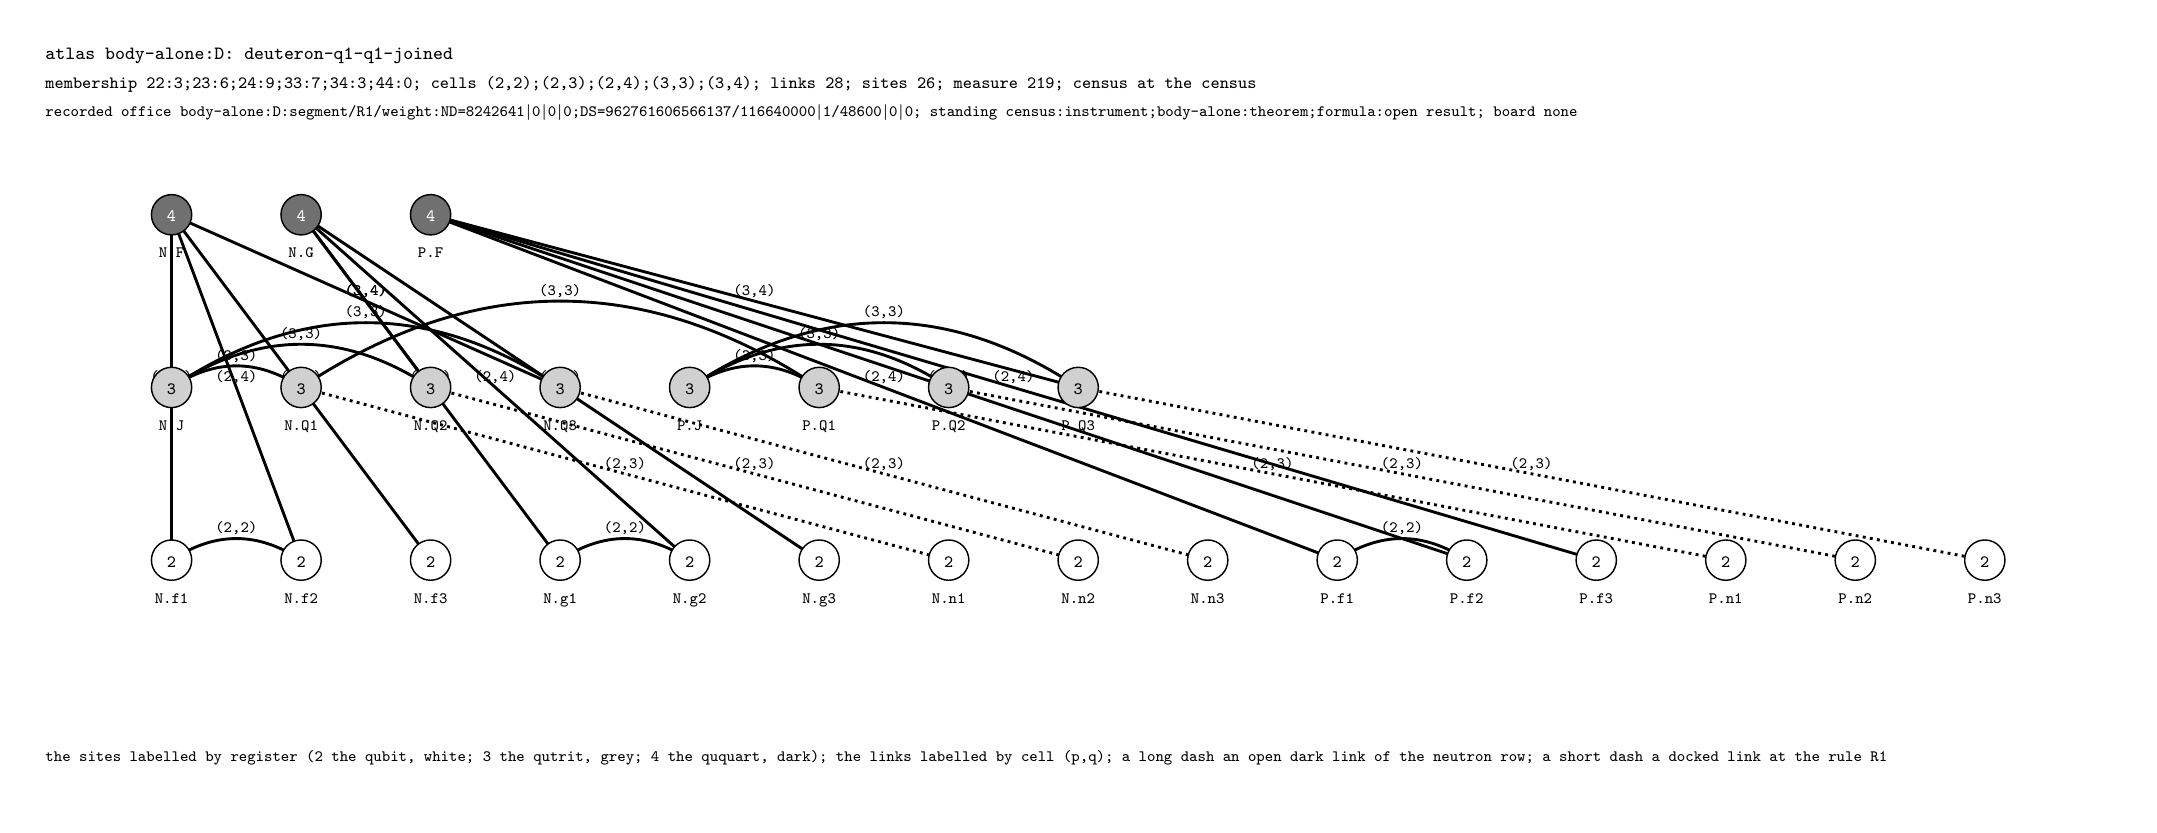
\begin{tikzpicture}[x=0.52pt,y=-0.52pt,baseline]
\clip (0,0) rectangle (1460,540);
\fill[white] (0,0) rectangle (1460,540);
\node[anchor=base west,inner sep=0pt,text=black,font=\fontsize{6.76}{8.112}\selectfont\ttfamily] at (12,22) {atlas body-alone:D: deuteron-q1-q1-joined};
\node[anchor=base west,inner sep=0pt,text=black,font=\fontsize{6.24}{7.488}\selectfont\ttfamily] at (12,42) {membership 22:3;23:6;24:9;33:7;34:3;44:0; cells (2,2);(2,3);(2,4);(3,3);(3,4); links 28; sites 26; measure 219; census at the census};
\node[anchor=base west,inner sep=0pt,text=black,font=\fontsize{5.72}{6.864}\selectfont\ttfamily] at (12,62) {recorded office body-alone:D:segment/R1/weight:ND=8242641\textbar{}0\textbar{}0\textbar{}0;DS=962761606566137/116640000\textbar{}1/48600\textbar{}0\textbar{}0; standing census:instrument;body-alone:theorem;formula:open result; board none};
\draw[draw=black,line width=1.04pt] (100,130) -- (370,250);
\node[anchor=base,inner sep=0pt,text=black,font=\fontsize{5.72}{6.864}\selectfont\ttfamily] at (235,186) {(3,4)};
\draw[draw=black,line width=1.04pt] (100,130) -- (100,370);
\node[anchor=base,inner sep=0pt,text=black,font=\fontsize{5.72}{6.864}\selectfont\ttfamily] at (100,246) {(2,4)};
\draw[draw=black,line width=1.04pt] (100,130) -- (190,370);
\node[anchor=base,inner sep=0pt,text=black,font=\fontsize{5.72}{6.864}\selectfont\ttfamily] at (145,246) {(2,4)};
\draw[draw=black,line width=1.04pt] (100,130) -- (280,370);
\node[anchor=base,inner sep=0pt,text=black,font=\fontsize{5.72}{6.864}\selectfont\ttfamily] at (190,246) {(2,4)};
\draw[draw=black,line width=1.04pt] (190,130) -- (280,250);
\node[anchor=base,inner sep=0pt,text=black,font=\fontsize{5.72}{6.864}\selectfont\ttfamily] at (235,186) {(3,4)};
\draw[draw=black,line width=1.04pt] (190,130) -- (370,370);
\node[anchor=base,inner sep=0pt,text=black,font=\fontsize{5.72}{6.864}\selectfont\ttfamily] at (280,246) {(2,4)};
\draw[draw=black,line width=1.04pt] (190,130) -- (460,370);
\node[anchor=base,inner sep=0pt,text=black,font=\fontsize{5.72}{6.864}\selectfont\ttfamily] at (325,246) {(2,4)};
\draw[draw=black,line width=1.04pt] (190,130) -- (550,370);
\node[anchor=base,inner sep=0pt,text=black,font=\fontsize{5.72}{6.864}\selectfont\ttfamily] at (370,246) {(2,4)};
\draw[draw=black,line width=1.04pt] (100,250) .. controls (130,230) and (160,230) .. (190,250);
\node[anchor=base,inner sep=0pt,text=black,font=\fontsize{5.72}{6.864}\selectfont\ttfamily] at (145,231) {(3,3)};
\draw[draw=black,line width=1.04pt] (100,250) .. controls (160,210) and (220,210) .. (280,250);
\node[anchor=base,inner sep=0pt,text=black,font=\fontsize{5.72}{6.864}\selectfont\ttfamily] at (190,216) {(3,3)};
\draw[draw=black,line width=1.04pt] (100,250) .. controls (190,190) and (280,190) .. (370,250);
\node[anchor=base,inner sep=0pt,text=black,font=\fontsize{5.72}{6.864}\selectfont\ttfamily] at (235,201) {(3,3)};
\draw[draw=black,line width=1.04pt,dash pattern=on 1.04pt off 1.56pt] (190,250) -- (640,370);
\node[anchor=base,inner sep=0pt,text=black,font=\fontsize{5.72}{6.864}\selectfont\ttfamily] at (415,306) {(2,3)};
\draw[draw=black,line width=1.04pt] (190,250) .. controls (310,170) and (430,170) .. (550,250);
\node[anchor=base,inner sep=0pt,text=black,font=\fontsize{5.72}{6.864}\selectfont\ttfamily] at (370,186) {(3,3)};
\draw[draw=black,line width=1.04pt,dash pattern=on 1.04pt off 1.56pt] (280,250) -- (730,370);
\node[anchor=base,inner sep=0pt,text=black,font=\fontsize{5.72}{6.864}\selectfont\ttfamily] at (505,306) {(2,3)};
\draw[draw=black,line width=1.04pt,dash pattern=on 1.04pt off 1.56pt] (370,250) -- (820,370);
\node[anchor=base,inner sep=0pt,text=black,font=\fontsize{5.72}{6.864}\selectfont\ttfamily] at (595,306) {(2,3)};
\draw[draw=black,line width=1.04pt] (100,370) .. controls (130,350) and (160,350) .. (190,370);
\node[anchor=base,inner sep=0pt,text=black,font=\fontsize{5.72}{6.864}\selectfont\ttfamily] at (145,351) {(2,2)};
\draw[draw=black,line width=1.04pt] (370,370) .. controls (400,350) and (430,350) .. (460,370);
\node[anchor=base,inner sep=0pt,text=black,font=\fontsize{5.72}{6.864}\selectfont\ttfamily] at (415,351) {(2,2)};
\draw[draw=black,line width=1.04pt] (280,130) -- (730,250);
\node[anchor=base,inner sep=0pt,text=black,font=\fontsize{5.72}{6.864}\selectfont\ttfamily] at (505,186) {(3,4)};
\draw[draw=black,line width=1.04pt] (280,130) -- (910,370);
\node[anchor=base,inner sep=0pt,text=black,font=\fontsize{5.72}{6.864}\selectfont\ttfamily] at (595,246) {(2,4)};
\draw[draw=black,line width=1.04pt] (280,130) -- (1000,370);
\node[anchor=base,inner sep=0pt,text=black,font=\fontsize{5.72}{6.864}\selectfont\ttfamily] at (640,246) {(2,4)};
\draw[draw=black,line width=1.04pt] (280,130) -- (1090,370);
\node[anchor=base,inner sep=0pt,text=black,font=\fontsize{5.72}{6.864}\selectfont\ttfamily] at (685,246) {(2,4)};
\draw[draw=black,line width=1.04pt] (460,250) .. controls (490,230) and (520,230) .. (550,250);
\node[anchor=base,inner sep=0pt,text=black,font=\fontsize{5.72}{6.864}\selectfont\ttfamily] at (505,231) {(3,3)};
\draw[draw=black,line width=1.04pt] (460,250) .. controls (520,210) and (580,210) .. (640,250);
\node[anchor=base,inner sep=0pt,text=black,font=\fontsize{5.72}{6.864}\selectfont\ttfamily] at (550,216) {(3,3)};
\draw[draw=black,line width=1.04pt] (460,250) .. controls (550,190) and (640,190) .. (730,250);
\node[anchor=base,inner sep=0pt,text=black,font=\fontsize{5.72}{6.864}\selectfont\ttfamily] at (595,201) {(3,3)};
\draw[draw=black,line width=1.04pt,dash pattern=on 1.04pt off 1.56pt] (550,250) -- (1180,370);
\node[anchor=base,inner sep=0pt,text=black,font=\fontsize{5.72}{6.864}\selectfont\ttfamily] at (865,306) {(2,3)};
\draw[draw=black,line width=1.04pt,dash pattern=on 1.04pt off 1.56pt] (640,250) -- (1270,370);
\node[anchor=base,inner sep=0pt,text=black,font=\fontsize{5.72}{6.864}\selectfont\ttfamily] at (955,306) {(2,3)};
\draw[draw=black,line width=1.04pt,dash pattern=on 1.04pt off 1.56pt] (730,250) -- (1360,370);
\node[anchor=base,inner sep=0pt,text=black,font=\fontsize{5.72}{6.864}\selectfont\ttfamily] at (1045,306) {(2,3)};
\draw[draw=black,line width=1.04pt] (910,370) .. controls (940,350) and (970,350) .. (1000,370);
\node[anchor=base,inner sep=0pt,text=black,font=\fontsize{5.72}{6.864}\selectfont\ttfamily] at (955,351) {(2,2)};
\filldraw[fill={rgb,255:red,112;green,112;blue,112},draw=black,line width=0.52pt] (100,130) circle (14);
\node[anchor=base,inner sep=0pt,text=white,font=\fontsize{6.24}{7.488}\selectfont\ttfamily] at (100,135) {4};
\node[anchor=base,inner sep=0pt,text=black,font=\fontsize{5.72}{6.864}\selectfont\ttfamily] at (100,160) {N.F};
\filldraw[fill={rgb,255:red,112;green,112;blue,112},draw=black,line width=0.52pt] (190,130) circle (14);
\node[anchor=base,inner sep=0pt,text=white,font=\fontsize{6.24}{7.488}\selectfont\ttfamily] at (190,135) {4};
\node[anchor=base,inner sep=0pt,text=black,font=\fontsize{5.72}{6.864}\selectfont\ttfamily] at (190,160) {N.G};
\filldraw[fill={rgb,255:red,208;green,208;blue,208},draw=black,line width=0.52pt] (100,250) circle (14);
\node[anchor=base,inner sep=0pt,text=black,font=\fontsize{6.24}{7.488}\selectfont\ttfamily] at (100,255) {3};
\node[anchor=base,inner sep=0pt,text=black,font=\fontsize{5.72}{6.864}\selectfont\ttfamily] at (100,280) {N.J};
\filldraw[fill={rgb,255:red,208;green,208;blue,208},draw=black,line width=0.52pt] (190,250) circle (14);
\node[anchor=base,inner sep=0pt,text=black,font=\fontsize{6.24}{7.488}\selectfont\ttfamily] at (190,255) {3};
\node[anchor=base,inner sep=0pt,text=black,font=\fontsize{5.72}{6.864}\selectfont\ttfamily] at (190,280) {N.Q1};
\filldraw[fill={rgb,255:red,208;green,208;blue,208},draw=black,line width=0.52pt] (280,250) circle (14);
\node[anchor=base,inner sep=0pt,text=black,font=\fontsize{6.24}{7.488}\selectfont\ttfamily] at (280,255) {3};
\node[anchor=base,inner sep=0pt,text=black,font=\fontsize{5.72}{6.864}\selectfont\ttfamily] at (280,280) {N.Q2};
\filldraw[fill={rgb,255:red,208;green,208;blue,208},draw=black,line width=0.52pt] (370,250) circle (14);
\node[anchor=base,inner sep=0pt,text=black,font=\fontsize{6.24}{7.488}\selectfont\ttfamily] at (370,255) {3};
\node[anchor=base,inner sep=0pt,text=black,font=\fontsize{5.72}{6.864}\selectfont\ttfamily] at (370,280) {N.Q3};
\filldraw[fill=white,draw=black,line width=0.52pt] (100,370) circle (14);
\node[anchor=base,inner sep=0pt,text=black,font=\fontsize{6.24}{7.488}\selectfont\ttfamily] at (100,375) {2};
\node[anchor=base,inner sep=0pt,text=black,font=\fontsize{5.72}{6.864}\selectfont\ttfamily] at (100,400) {N.f1};
\filldraw[fill=white,draw=black,line width=0.52pt] (190,370) circle (14);
\node[anchor=base,inner sep=0pt,text=black,font=\fontsize{6.24}{7.488}\selectfont\ttfamily] at (190,375) {2};
\node[anchor=base,inner sep=0pt,text=black,font=\fontsize{5.72}{6.864}\selectfont\ttfamily] at (190,400) {N.f2};
\filldraw[fill=white,draw=black,line width=0.52pt] (280,370) circle (14);
\node[anchor=base,inner sep=0pt,text=black,font=\fontsize{6.24}{7.488}\selectfont\ttfamily] at (280,375) {2};
\node[anchor=base,inner sep=0pt,text=black,font=\fontsize{5.72}{6.864}\selectfont\ttfamily] at (280,400) {N.f3};
\filldraw[fill=white,draw=black,line width=0.52pt] (370,370) circle (14);
\node[anchor=base,inner sep=0pt,text=black,font=\fontsize{6.24}{7.488}\selectfont\ttfamily] at (370,375) {2};
\node[anchor=base,inner sep=0pt,text=black,font=\fontsize{5.72}{6.864}\selectfont\ttfamily] at (370,400) {N.g1};
\filldraw[fill=white,draw=black,line width=0.52pt] (460,370) circle (14);
\node[anchor=base,inner sep=0pt,text=black,font=\fontsize{6.24}{7.488}\selectfont\ttfamily] at (460,375) {2};
\node[anchor=base,inner sep=0pt,text=black,font=\fontsize{5.72}{6.864}\selectfont\ttfamily] at (460,400) {N.g2};
\filldraw[fill=white,draw=black,line width=0.52pt] (550,370) circle (14);
\node[anchor=base,inner sep=0pt,text=black,font=\fontsize{6.24}{7.488}\selectfont\ttfamily] at (550,375) {2};
\node[anchor=base,inner sep=0pt,text=black,font=\fontsize{5.72}{6.864}\selectfont\ttfamily] at (550,400) {N.g3};
\filldraw[fill=white,draw=black,line width=0.52pt] (640,370) circle (14);
\node[anchor=base,inner sep=0pt,text=black,font=\fontsize{6.24}{7.488}\selectfont\ttfamily] at (640,375) {2};
\node[anchor=base,inner sep=0pt,text=black,font=\fontsize{5.72}{6.864}\selectfont\ttfamily] at (640,400) {N.n1};
\filldraw[fill=white,draw=black,line width=0.52pt] (730,370) circle (14);
\node[anchor=base,inner sep=0pt,text=black,font=\fontsize{6.24}{7.488}\selectfont\ttfamily] at (730,375) {2};
\node[anchor=base,inner sep=0pt,text=black,font=\fontsize{5.72}{6.864}\selectfont\ttfamily] at (730,400) {N.n2};
\filldraw[fill=white,draw=black,line width=0.52pt] (820,370) circle (14);
\node[anchor=base,inner sep=0pt,text=black,font=\fontsize{6.24}{7.488}\selectfont\ttfamily] at (820,375) {2};
\node[anchor=base,inner sep=0pt,text=black,font=\fontsize{5.72}{6.864}\selectfont\ttfamily] at (820,400) {N.n3};
\filldraw[fill={rgb,255:red,112;green,112;blue,112},draw=black,line width=0.52pt] (280,130) circle (14);
\node[anchor=base,inner sep=0pt,text=white,font=\fontsize{6.24}{7.488}\selectfont\ttfamily] at (280,135) {4};
\node[anchor=base,inner sep=0pt,text=black,font=\fontsize{5.72}{6.864}\selectfont\ttfamily] at (280,160) {P.F};
\filldraw[fill={rgb,255:red,208;green,208;blue,208},draw=black,line width=0.52pt] (460,250) circle (14);
\node[anchor=base,inner sep=0pt,text=black,font=\fontsize{6.24}{7.488}\selectfont\ttfamily] at (460,255) {3};
\node[anchor=base,inner sep=0pt,text=black,font=\fontsize{5.72}{6.864}\selectfont\ttfamily] at (460,280) {P.J};
\filldraw[fill={rgb,255:red,208;green,208;blue,208},draw=black,line width=0.52pt] (550,250) circle (14);
\node[anchor=base,inner sep=0pt,text=black,font=\fontsize{6.24}{7.488}\selectfont\ttfamily] at (550,255) {3};
\node[anchor=base,inner sep=0pt,text=black,font=\fontsize{5.72}{6.864}\selectfont\ttfamily] at (550,280) {P.Q1};
\filldraw[fill={rgb,255:red,208;green,208;blue,208},draw=black,line width=0.52pt] (640,250) circle (14);
\node[anchor=base,inner sep=0pt,text=black,font=\fontsize{6.24}{7.488}\selectfont\ttfamily] at (640,255) {3};
\node[anchor=base,inner sep=0pt,text=black,font=\fontsize{5.72}{6.864}\selectfont\ttfamily] at (640,280) {P.Q2};
\filldraw[fill={rgb,255:red,208;green,208;blue,208},draw=black,line width=0.52pt] (730,250) circle (14);
\node[anchor=base,inner sep=0pt,text=black,font=\fontsize{6.24}{7.488}\selectfont\ttfamily] at (730,255) {3};
\node[anchor=base,inner sep=0pt,text=black,font=\fontsize{5.72}{6.864}\selectfont\ttfamily] at (730,280) {P.Q3};
\filldraw[fill=white,draw=black,line width=0.52pt] (910,370) circle (14);
\node[anchor=base,inner sep=0pt,text=black,font=\fontsize{6.24}{7.488}\selectfont\ttfamily] at (910,375) {2};
\node[anchor=base,inner sep=0pt,text=black,font=\fontsize{5.72}{6.864}\selectfont\ttfamily] at (910,400) {P.f1};
\filldraw[fill=white,draw=black,line width=0.52pt] (1000,370) circle (14);
\node[anchor=base,inner sep=0pt,text=black,font=\fontsize{6.24}{7.488}\selectfont\ttfamily] at (1000,375) {2};
\node[anchor=base,inner sep=0pt,text=black,font=\fontsize{5.72}{6.864}\selectfont\ttfamily] at (1000,400) {P.f2};
\filldraw[fill=white,draw=black,line width=0.52pt] (1090,370) circle (14);
\node[anchor=base,inner sep=0pt,text=black,font=\fontsize{6.24}{7.488}\selectfont\ttfamily] at (1090,375) {2};
\node[anchor=base,inner sep=0pt,text=black,font=\fontsize{5.72}{6.864}\selectfont\ttfamily] at (1090,400) {P.f3};
\filldraw[fill=white,draw=black,line width=0.52pt] (1180,370) circle (14);
\node[anchor=base,inner sep=0pt,text=black,font=\fontsize{6.24}{7.488}\selectfont\ttfamily] at (1180,375) {2};
\node[anchor=base,inner sep=0pt,text=black,font=\fontsize{5.72}{6.864}\selectfont\ttfamily] at (1180,400) {P.n1};
\filldraw[fill=white,draw=black,line width=0.52pt] (1270,370) circle (14);
\node[anchor=base,inner sep=0pt,text=black,font=\fontsize{6.24}{7.488}\selectfont\ttfamily] at (1270,375) {2};
\node[anchor=base,inner sep=0pt,text=black,font=\fontsize{5.72}{6.864}\selectfont\ttfamily] at (1270,400) {P.n2};
\filldraw[fill=white,draw=black,line width=0.52pt] (1360,370) circle (14);
\node[anchor=base,inner sep=0pt,text=black,font=\fontsize{6.24}{7.488}\selectfont\ttfamily] at (1360,375) {2};
\node[anchor=base,inner sep=0pt,text=black,font=\fontsize{5.72}{6.864}\selectfont\ttfamily] at (1360,400) {P.n3};
\node[anchor=base west,inner sep=0pt,text=black,font=\fontsize{5.72}{6.864}\selectfont\ttfamily] at (12,510) {the sites labelled by register (2 the qubit, white; 3 the qutrit, grey; 4 the ququart, dark); the links labelled by cell (p,q); a long dash an open dark link of the neutron row; a short dash a docked link at the rule R1};
\end{tikzpicture}\end{adjustbox}
\caption{\texttt{deuteron-q1-q1-joined}, deuteron joined: 26 sites, 28 links, the measure 219; the links at the cells (2,2), (2,3), (2,4), (3,3), (3,4); the membership 22:3; 23:6; 24:9; 33:7; 34:3; 44:0; 6 docked links at the rule R1 (P.Q1-P.n1; P.Q2-P.n2; P.Q3-P.n3; N.Q1-N.n1; N.Q2-N.n2; N.Q3-N.n3); at the census of the six cells. Drawn at the anatomy atlas as its web, the sites labeled by register and the links by cell, from the the body-alone office rule.}\label{fig:VIII-2-D537322-deuteron-q1-q1-joined-b6dadc}
\begin{center}\footnotesize\begin{adjustbox}{max width=\linewidth}\begin{tabular}{p{0.26\textwidth}p{0.68\textwidth}}\toprule
recorded office (the slot-count row) & the read o-nd of the formula row: the first power 2871; the office \texttt{8242641\textbar{}0\textbar{}0\textbar{}0}; against the formula with the slot count equal; the slot total 0; dark links 22; hubs P.F; N.F; N.G; dressing 9 \\
mass register (the mass-register row) & the read BD: the class touching the ququart; the first power 4941; the office \texttt{15 999 659 899 116 267/655360000\textbar{}1983/50\textbar{}14163873/32768000\textbar{}0}; nonzero; met yes; hubs N.F; N.G; P.F; in-legs P.Q3-P.F; N.Q3-N.F; N.Q2-N.G; dressing 27; ports P.Q1-P.n1; P.Q2-P.n2; P.Q3-P.n3; P.f-p.f3; N.Q1-N.n1; N.Q2-N.n2; N.Q3-N.n3; N.f-n.f3; N.g-n.g3 \\
junction registers (the hadron row) & the read ND: junctions P.J; P.Q1; P.Q3; N.J; N.Q1; N.Q2; N.Q3; the share one third per leg; the registers at the share 219, struck 183, mono 5913, the hub spelling 1971; against the cells none; none; none; none, none \\
\bottomrule\end{tabular}\end{adjustbox}\end{center}
\end{figure}
\begin{figure}[H]\centering
\begin{adjustbox}{max width=\linewidth}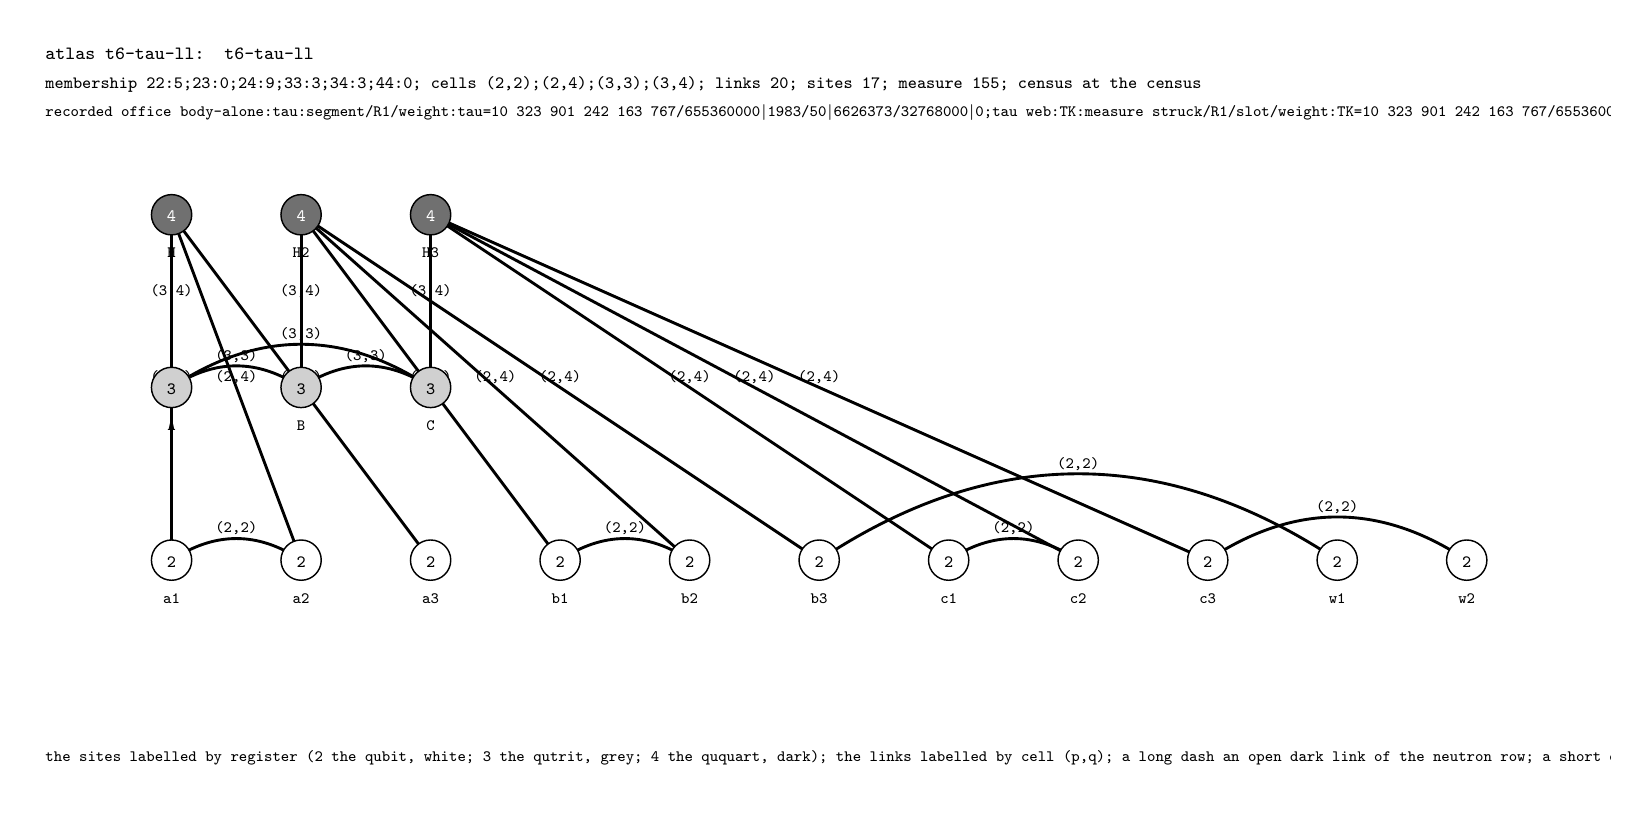
\begin{tikzpicture}[x=0.52pt,y=-0.52pt,baseline]
\clip (0,0) rectangle (1100,540);
\fill[white] (0,0) rectangle (1100,540);
\node[anchor=base west,inner sep=0pt,text=black,font=\fontsize{6.76}{8.112}\selectfont\ttfamily] at (12,22) {atlas t6-tau-ll: t6-tau-ll};
\node[anchor=base west,inner sep=0pt,text=black,font=\fontsize{6.24}{7.488}\selectfont\ttfamily] at (12,42) {membership 22:5;23:0;24:9;33:3;34:3;44:0; cells (2,2);(2,4);(3,3);(3,4); links 20; sites 17; measure 155; census at the census};
\node[anchor=base west,inner sep=0pt,text=black,font=\fontsize{5.72}{6.864}\selectfont\ttfamily] at (12,62) {recorded office body-alone:tau:segment/R1/weight:tau=10 323 901 242 163 767/655360000\textbar{}1983/50\textbar{}6626373/32768000\textbar{}0;tau web:TK:measure struck/R1/slot/weight:TK=10 323 901 242 163 767/655360000\textbar{}1983/50\textbar{}6626373/32768000\textbar{}0; standing census:instrument;body-alone:theorem;formula:open result;tau web:theorem;roster:roster word; board tau};
\draw[draw=black,line width=1.04pt] (100,250) .. controls (130,230) and (160,230) .. (190,250);
\node[anchor=base,inner sep=0pt,text=black,font=\fontsize{5.72}{6.864}\selectfont\ttfamily] at (145,231) {(3,3)};
\draw[draw=black,line width=1.04pt] (100,250) .. controls (160,210) and (220,210) .. (280,250);
\node[anchor=base,inner sep=0pt,text=black,font=\fontsize{5.72}{6.864}\selectfont\ttfamily] at (190,216) {(3,3)};
\draw[draw=black,line width=1.04pt] (100,250) -- (100,130);
\node[anchor=base,inner sep=0pt,text=black,font=\fontsize{5.72}{6.864}\selectfont\ttfamily] at (100,186) {(3,4)};
\draw[draw=black,line width=1.04pt] (190,250) .. controls (220,230) and (250,230) .. (280,250);
\node[anchor=base,inner sep=0pt,text=black,font=\fontsize{5.72}{6.864}\selectfont\ttfamily] at (235,231) {(3,3)};
\draw[draw=black,line width=1.04pt] (190,250) -- (190,130);
\node[anchor=base,inner sep=0pt,text=black,font=\fontsize{5.72}{6.864}\selectfont\ttfamily] at (190,186) {(3,4)};
\draw[draw=black,line width=1.04pt] (280,250) -- (280,130);
\node[anchor=base,inner sep=0pt,text=black,font=\fontsize{5.72}{6.864}\selectfont\ttfamily] at (280,186) {(3,4)};
\draw[draw=black,line width=1.04pt] (100,130) -- (100,370);
\node[anchor=base,inner sep=0pt,text=black,font=\fontsize{5.72}{6.864}\selectfont\ttfamily] at (100,246) {(2,4)};
\draw[draw=black,line width=1.04pt] (100,130) -- (190,370);
\node[anchor=base,inner sep=0pt,text=black,font=\fontsize{5.72}{6.864}\selectfont\ttfamily] at (145,246) {(2,4)};
\draw[draw=black,line width=1.04pt] (100,130) -- (280,370);
\node[anchor=base,inner sep=0pt,text=black,font=\fontsize{5.72}{6.864}\selectfont\ttfamily] at (190,246) {(2,4)};
\draw[draw=black,line width=1.04pt] (190,130) -- (370,370);
\node[anchor=base,inner sep=0pt,text=black,font=\fontsize{5.72}{6.864}\selectfont\ttfamily] at (280,246) {(2,4)};
\draw[draw=black,line width=1.04pt] (190,130) -- (460,370);
\node[anchor=base,inner sep=0pt,text=black,font=\fontsize{5.72}{6.864}\selectfont\ttfamily] at (325,246) {(2,4)};
\draw[draw=black,line width=1.04pt] (190,130) -- (550,370);
\node[anchor=base,inner sep=0pt,text=black,font=\fontsize{5.72}{6.864}\selectfont\ttfamily] at (370,246) {(2,4)};
\draw[draw=black,line width=1.04pt] (280,130) -- (640,370);
\node[anchor=base,inner sep=0pt,text=black,font=\fontsize{5.72}{6.864}\selectfont\ttfamily] at (460,246) {(2,4)};
\draw[draw=black,line width=1.04pt] (280,130) -- (730,370);
\node[anchor=base,inner sep=0pt,text=black,font=\fontsize{5.72}{6.864}\selectfont\ttfamily] at (505,246) {(2,4)};
\draw[draw=black,line width=1.04pt] (280,130) -- (820,370);
\node[anchor=base,inner sep=0pt,text=black,font=\fontsize{5.72}{6.864}\selectfont\ttfamily] at (550,246) {(2,4)};
\draw[draw=black,line width=1.04pt] (100,370) .. controls (130,350) and (160,350) .. (190,370);
\node[anchor=base,inner sep=0pt,text=black,font=\fontsize{5.72}{6.864}\selectfont\ttfamily] at (145,351) {(2,2)};
\draw[draw=black,line width=1.04pt] (370,370) .. controls (400,350) and (430,350) .. (460,370);
\node[anchor=base,inner sep=0pt,text=black,font=\fontsize{5.72}{6.864}\selectfont\ttfamily] at (415,351) {(2,2)};
\draw[draw=black,line width=1.04pt] (550,370) .. controls (670,290) and (790,290) .. (910,370);
\node[anchor=base,inner sep=0pt,text=black,font=\fontsize{5.72}{6.864}\selectfont\ttfamily] at (730,306) {(2,2)};
\draw[draw=black,line width=1.04pt] (640,370) .. controls (670,350) and (700,350) .. (730,370);
\node[anchor=base,inner sep=0pt,text=black,font=\fontsize{5.72}{6.864}\selectfont\ttfamily] at (685,351) {(2,2)};
\draw[draw=black,line width=1.04pt] (820,370) .. controls (880,330) and (940,330) .. (1000,370);
\node[anchor=base,inner sep=0pt,text=black,font=\fontsize{5.72}{6.864}\selectfont\ttfamily] at (910,336) {(2,2)};
\filldraw[fill={rgb,255:red,208;green,208;blue,208},draw=black,line width=0.52pt] (100,250) circle (14);
\node[anchor=base,inner sep=0pt,text=black,font=\fontsize{6.24}{7.488}\selectfont\ttfamily] at (100,255) {3};
\node[anchor=base,inner sep=0pt,text=black,font=\fontsize{5.72}{6.864}\selectfont\ttfamily] at (100,280) {A};
\filldraw[fill={rgb,255:red,208;green,208;blue,208},draw=black,line width=0.52pt] (190,250) circle (14);
\node[anchor=base,inner sep=0pt,text=black,font=\fontsize{6.24}{7.488}\selectfont\ttfamily] at (190,255) {3};
\node[anchor=base,inner sep=0pt,text=black,font=\fontsize{5.72}{6.864}\selectfont\ttfamily] at (190,280) {B};
\filldraw[fill={rgb,255:red,208;green,208;blue,208},draw=black,line width=0.52pt] (280,250) circle (14);
\node[anchor=base,inner sep=0pt,text=black,font=\fontsize{6.24}{7.488}\selectfont\ttfamily] at (280,255) {3};
\node[anchor=base,inner sep=0pt,text=black,font=\fontsize{5.72}{6.864}\selectfont\ttfamily] at (280,280) {C};
\filldraw[fill={rgb,255:red,112;green,112;blue,112},draw=black,line width=0.52pt] (100,130) circle (14);
\node[anchor=base,inner sep=0pt,text=white,font=\fontsize{6.24}{7.488}\selectfont\ttfamily] at (100,135) {4};
\node[anchor=base,inner sep=0pt,text=black,font=\fontsize{5.72}{6.864}\selectfont\ttfamily] at (100,160) {H};
\filldraw[fill={rgb,255:red,112;green,112;blue,112},draw=black,line width=0.52pt] (190,130) circle (14);
\node[anchor=base,inner sep=0pt,text=white,font=\fontsize{6.24}{7.488}\selectfont\ttfamily] at (190,135) {4};
\node[anchor=base,inner sep=0pt,text=black,font=\fontsize{5.72}{6.864}\selectfont\ttfamily] at (190,160) {H2};
\filldraw[fill={rgb,255:red,112;green,112;blue,112},draw=black,line width=0.52pt] (280,130) circle (14);
\node[anchor=base,inner sep=0pt,text=white,font=\fontsize{6.24}{7.488}\selectfont\ttfamily] at (280,135) {4};
\node[anchor=base,inner sep=0pt,text=black,font=\fontsize{5.72}{6.864}\selectfont\ttfamily] at (280,160) {H3};
\filldraw[fill=white,draw=black,line width=0.52pt] (100,370) circle (14);
\node[anchor=base,inner sep=0pt,text=black,font=\fontsize{6.24}{7.488}\selectfont\ttfamily] at (100,375) {2};
\node[anchor=base,inner sep=0pt,text=black,font=\fontsize{5.72}{6.864}\selectfont\ttfamily] at (100,400) {a1};
\filldraw[fill=white,draw=black,line width=0.52pt] (190,370) circle (14);
\node[anchor=base,inner sep=0pt,text=black,font=\fontsize{6.24}{7.488}\selectfont\ttfamily] at (190,375) {2};
\node[anchor=base,inner sep=0pt,text=black,font=\fontsize{5.72}{6.864}\selectfont\ttfamily] at (190,400) {a2};
\filldraw[fill=white,draw=black,line width=0.52pt] (280,370) circle (14);
\node[anchor=base,inner sep=0pt,text=black,font=\fontsize{6.24}{7.488}\selectfont\ttfamily] at (280,375) {2};
\node[anchor=base,inner sep=0pt,text=black,font=\fontsize{5.72}{6.864}\selectfont\ttfamily] at (280,400) {a3};
\filldraw[fill=white,draw=black,line width=0.52pt] (370,370) circle (14);
\node[anchor=base,inner sep=0pt,text=black,font=\fontsize{6.24}{7.488}\selectfont\ttfamily] at (370,375) {2};
\node[anchor=base,inner sep=0pt,text=black,font=\fontsize{5.72}{6.864}\selectfont\ttfamily] at (370,400) {b1};
\filldraw[fill=white,draw=black,line width=0.52pt] (460,370) circle (14);
\node[anchor=base,inner sep=0pt,text=black,font=\fontsize{6.24}{7.488}\selectfont\ttfamily] at (460,375) {2};
\node[anchor=base,inner sep=0pt,text=black,font=\fontsize{5.72}{6.864}\selectfont\ttfamily] at (460,400) {b2};
\filldraw[fill=white,draw=black,line width=0.52pt] (550,370) circle (14);
\node[anchor=base,inner sep=0pt,text=black,font=\fontsize{6.24}{7.488}\selectfont\ttfamily] at (550,375) {2};
\node[anchor=base,inner sep=0pt,text=black,font=\fontsize{5.72}{6.864}\selectfont\ttfamily] at (550,400) {b3};
\filldraw[fill=white,draw=black,line width=0.52pt] (640,370) circle (14);
\node[anchor=base,inner sep=0pt,text=black,font=\fontsize{6.24}{7.488}\selectfont\ttfamily] at (640,375) {2};
\node[anchor=base,inner sep=0pt,text=black,font=\fontsize{5.72}{6.864}\selectfont\ttfamily] at (640,400) {c1};
\filldraw[fill=white,draw=black,line width=0.52pt] (730,370) circle (14);
\node[anchor=base,inner sep=0pt,text=black,font=\fontsize{6.24}{7.488}\selectfont\ttfamily] at (730,375) {2};
\node[anchor=base,inner sep=0pt,text=black,font=\fontsize{5.72}{6.864}\selectfont\ttfamily] at (730,400) {c2};
\filldraw[fill=white,draw=black,line width=0.52pt] (820,370) circle (14);
\node[anchor=base,inner sep=0pt,text=black,font=\fontsize{6.24}{7.488}\selectfont\ttfamily] at (820,375) {2};
\node[anchor=base,inner sep=0pt,text=black,font=\fontsize{5.72}{6.864}\selectfont\ttfamily] at (820,400) {c3};
\filldraw[fill=white,draw=black,line width=0.52pt] (910,370) circle (14);
\node[anchor=base,inner sep=0pt,text=black,font=\fontsize{6.24}{7.488}\selectfont\ttfamily] at (910,375) {2};
\node[anchor=base,inner sep=0pt,text=black,font=\fontsize{5.72}{6.864}\selectfont\ttfamily] at (910,400) {w1};
\filldraw[fill=white,draw=black,line width=0.52pt] (1000,370) circle (14);
\node[anchor=base,inner sep=0pt,text=black,font=\fontsize{6.24}{7.488}\selectfont\ttfamily] at (1000,375) {2};
\node[anchor=base,inner sep=0pt,text=black,font=\fontsize{5.72}{6.864}\selectfont\ttfamily] at (1000,400) {w2};
\node[anchor=base west,inner sep=0pt,text=black,font=\fontsize{5.72}{6.864}\selectfont\ttfamily] at (12,510) {the sites labelled by register (2 the qubit, white; 3 the qutrit, grey; 4 the ququart, dark); the links labelled by cell (p,q); a long dash an open dark link of the neutron row; a short dash a docked link at the rule R1};
\end{tikzpicture}\end{adjustbox}
\caption{\texttt{t6-tau-ll} (the tau), recorded body, roster web: 17 sites, 20 links, the measure 155; the links at the cells (2,2), (2,4), (3,3), (3,4); the membership 22:5; 23:0; 24:9; 33:3; 34:3; 44:0; dock-free at the rule R1; at the census of the six cells. Drawn at the anatomy atlas as its web, the sites labeled by register and the links by cell, from the the body-alone office rule.}\label{fig:VIII-2-D537322-t6-tau-ll-cfed05}
\begin{center}\footnotesize\begin{adjustbox}{max width=\linewidth}\begin{tabular}{p{0.26\textwidth}p{0.68\textwidth}}\toprule
recorded office (the slot-count row) & the read o-tau of the formula row: the first power 3969; the office \texttt{10 323 901 242 163 767/655360000\textbar{}1983/50\textbar{}6626373/32768000\textbar{}0}; against the formula with the slot count equal; the slot total 0; dark links 20; hubs H; H2; H3; dressing 27 \\
mass register (the mass-register row) & the read btau: the class touching the ququart; the first power 3969; the office \texttt{10 323 901 242 163 767/655360000\textbar{}1983/50\textbar{}6626373/32768000\textbar{}0}; nonzero; met yes; hubs H; H2; H3; in-legs h-a; H2-B; H3-C; dressing 27; ports H-a3; w1-b3; w2-c3 \\
lepton-form office (the lepton row) & the read l-tk: the first power 3969; the office \texttt{10 323 901 242 163 767/655360000\textbar{}1983/50\textbar{}6626373/32768000\textbar{}0}; against the cell equal; dark links 20 \\
\bottomrule\end{tabular}\end{adjustbox}\end{center}
\end{figure}
\begin{figure}[h]
\centering
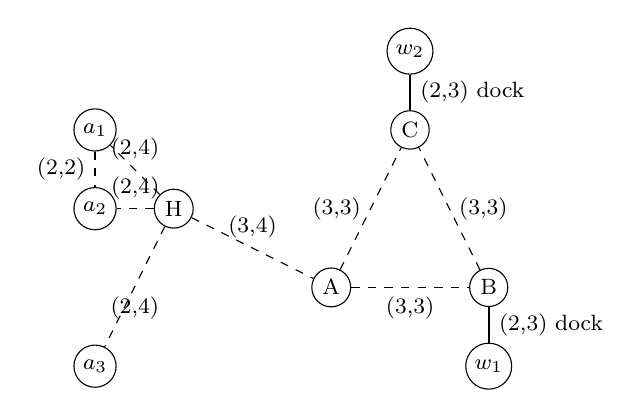
\begin{tikzpicture}[every node/.style={font=\footnotesize}]
\node[circle,draw,inner sep=2pt] (A) at (0,0) {A};
\node[circle,draw,inner sep=2pt] (B) at (2,0) {B};
\node[circle,draw,inner sep=2pt] (C) at (1,2) {C};
\node[circle,draw,inner sep=2pt] (H) at (-2,1) {H};
\node[circle,draw,inner sep=2pt] (a1) at (-3,2) {$a_1$};
\node[circle,draw,inner sep=2pt] (a2) at (-3,1) {$a_2$};
\node[circle,draw,inner sep=2pt] (a3) at (-3,-1) {$a_3$};
\node[circle,draw,inner sep=2pt] (w1) at (2,-1) {$w_1$};
\node[circle,draw,inner sep=2pt] (w2) at (1,3) {$w_2$};
\draw[dashed] (A) -- node[below] {(3,3)} (B);
\draw[dashed] (B) -- node[right] {(3,3)} (C);
\draw[dashed] (A) -- node[left] {(3,3)} (C);
\draw[dashed] (H) -- node[above] {(3,4)} (A);
\draw[dashed] (H) -- node[above] {(2,4)} (a1);
\draw[dashed] (H) -- node[above] {(2,4)} (a2);
\draw[dashed] (H) -- node[below] {(2,4)} (a3);
\draw[dashed] (a1) -- node[left] {(2,2)} (a2);
\draw[thick] (B) -- node[right] {(2,3) dock} (w1);
\draw[thick] (C) -- node[right] {(2,3) dock} (w2);
\end{tikzpicture}
\caption{The two-dock electron web of the body-alone rule. Nine sites and ten links, each link labeled by its genre. The two (2,3) docks at $w_1$ and $w_2$ carry the read, and the eight dashed links of the other genres form the dark set that closes at the closure term.}
\end{figure}
\par\medskip\noindent{\itshape Beyond the first power, the next chapter reads the next terms.}\label{narr:close:8-2}\par
\section{The next terms and the unstable rows}\label{mod:VIII-3-next-terms-and-the-unstable-rows}
\chdesig{10-3}{8-3}{VIII-3-next-terms-and-the-unstable-rows}{VIII-3-next-terms-and-the-unstable-rows}
\label{narr:open:8-3}Theorem~196.1 reads the next terms and the unstable rows, and Theorem~196.2, a theorem, the lepton joined face at the open attach site.
\begin{chconditional}[The next terms and the unstable rows]\label{box:VIII-3-next-terms-and-the-unstable-rows:1}
Conditional on the results this entry rests on, among them first power as the act readout sum and mass as the direct two-exchange sum at the common support, each at its own standing. At the cells of the ladder, the link-weight placement and the dock spelling, with the unit the dock-struck electron first power, every next term is an exact object with a definite sign: positive at the muon office and at the tau office and negative at the Koide relation, the next term at the muon office the closure object over the unit squared, an element of the field of the two roots.
\end{chconditional}
\chstanding{conditional theorem}
\chdeps{Definitions 1.1 to 1.6, Theorem 152.1 and Theorems 185.1 to 185.12}{Open result 157.1 and Theorems 162.1 and 162.2}
\begin{chtheorem}[The lepton joined face at the open attach site]\label{box:VIII-3-next-terms-and-the-unstable-rows:2}
Every site of the tau is typed under the definition of open, the far end of the entered link open exactly when the near end is the larger: twelve of the seventeen sites are open attach sites, and the joined face of the tau is defined at one of them, the body alone at the first order and the second-order object an exact element of the field.
\end{chtheorem}
\chstanding{theorem}
\chdeps{Definitions 1.1 to 1.6, Theorem 152.1 and Theorems 185.1 to 185.12}{Open result 157.1 and Theorems 162.1 and 162.2}
The next term is computed at the link-weight placement at every cell of the ladder at the dock spelling, and its sign is decided exactly through the subfield of the first root. Every site of the tau is typed at the definition of open with the transport-pair table re-met at the dimension rule, and the joined face is taken at an open site. The one open question of the chapter, the unstable-row correction as the open-move readout, is a reading that was tried and parted at its named step, and the object the decay releases stands at its own chapter.
\begin{chbridge}
In quantum field theory the mass of a body is corrected order by order by its self-energy, the next term of the expansion a loop integral with a definite sign at each order \cite{Weinberg1995}, and an unstable body carries a width beside its mass, the pole of its propagator moved off the real axis by the open decay channels \cite{BreitWigner1936}. The correspondence is by name.
\end{chbridge}
\begin{chproof}[exhaustive census with its exact part]
\textit{The premises.} The axiom and the six definitions of Section~\ref{mod:FRAMEWORK}, definitions. The first power and the placement per web of Section~\ref{mod:VIII-1-mass-unit-and-the-first-power}, theorems. The lepton ladder as hub assemblies of Section~\ref{mod:V-10-lepton-ladder-as-hub-assemblies}, a theorem. The Koide reading at the dock unit and the next-term reading, two open readings consumed at their tables. The chain from the axiom to this result is seven chapters deep.

\textit{The exact part: the next term at an office.} The unit is the dock-struck electron first power, $u=67$, re-met at eleven cells of the results above. At a lepton body with the first power $S_1$ and the direct two-exchange sum $S_2$, from the direct sum and the first power, by subtraction, we obtain the closure object $S_2-S_1^{2}$. From the first power and the unit, by division, we obtain the first-order office $S_1^{2}/u^{2}$. From the closure object and the unit, by division, we obtain the next term
\begin{equation}
n=\frac{S_2-S_1^{2}}{u^{2}} ,
\end{equation}
an element of the ring with basis one, root two and root three. From the first-order office and the next term, by addition, we obtain the order-two office $S_2/u^{2}$. The smallest instance is the electron at its own unit. The first-order office is $1$ and the next term is the closure ratio of the first-power result,
\begin{equation}
n_{e}=\tfrac{13\,708\,610\,839}{2\,144\,653\,148\,160\,000}+\tfrac{661}{163\,624\,050}\sqrt{2}+\tfrac{5\,977\,541}{107\,232\,657\,408\,000}\sqrt{3},
\end{equation}
positive. At the muon, against the first-order office $927\,369/4489$, the next term is
\begin{equation}
n_{\mu}=\tfrac{39\,502\,907\,303}{26\,477\,199\,360\,000}+\tfrac{649}{673\,350}\sqrt{2}+\tfrac{6\,301\,957}{1\,323\,859\,968\,000}\sqrt{3},
\end{equation}
and at the tau, against $15\,752\,961/4489$,
\begin{equation}
n_{\tau}=\tfrac{65\,297\,203\,767}{2\,941\,911\,040\,000}+\tfrac{3233}{224\,450}\sqrt{2}+\tfrac{6\,626\,373}{147\,095\,552\,000}\sqrt{3},
\end{equation}
each positive, the sign certified by an exact bracket at forty digits that excludes zero. The order-two offices equal the direct sums over the unit squared of the first-power result at the three bodies. At the Koide relation the three dock-spelled direct sums have roots outside the field of the two roots (none of three in the field, decided exactly through the subfield of root two), the three adjoined roots independent, so the relation is an exact object of the formal tower less the first-order relation $16\,684\,819/24\,990\,001$, whose departure from two thirds, $74\,455/74\,970\,003$, is positive. Its next term is negative, the direct bracket
\begin{equation}
-\tfrac{1\,567\,258\,759\,542\,141\,982\,137\,839\,353\,220\,402}{10^{40}}\ \text{to}\ -\tfrac{1\,567\,258\,759\,542\,141\,982\,137\,839\,353\,220\,400}{10^{40}}
\end{equation}
overlapping the tower-route bracket.

\textit{The census.} The set counted is the derived cells, the five bodies at two placements (the link weight and the body weight) and two readings of the electron, twenty-four office cells, and the eight relation cells at both ladders and placements. The property tested at each office cell is whether the next term is a nonzero exact element of the field with its sign certified by a bracket excluding zero, and at each relation cell whether the next term of the Koide relation is such an object. The counts are 24 of 24 office cells defined and positive, 8 of 8 relation cells certified, the first undecided cell none, and the triple at the derived cells positive, positive, negative. Beside, at the body-weight placement the triple reads positive, positive, positive, and at the derived ladder positive, positive, negative at the link weight. Every one is printed beside.

\textit{The check.} Setting the unit to the hub first power $201$ moves every office but the electron at its dock reading. Setting the placement to the body weight moves the Koide sign from negative to positive and no office sign. Striking the next term moves no first-order cell. Replacing the ladder by the derived ladder moves thirty-one of fifty-seven compared keys. Each alteration moves the cells it names. The result was reproduced by an independent route, two engines of different construction agreeing at every cell at both runs, with the dock table and unit of the first-power result, the cells of the Koide reading and the sums of the two-exchange result as the controls.
\chcert{24}
\end{chproof}
\begin{figure}[h]
\centering
\begin{adjustbox}{max width=\linewidth}\begin{tabular}{lll}
\hline
cell & first-order object & sign of the next term \\
\hline
electron at the hub reading & $9$ & positive \\
electron at the dock reading & $1$ & positive \\
muon office & $927\,369/4489$ & positive \\
tau office & $15\,752\,961/4489$ & positive \\
Koide relation at the dock spelling & $16\,684\,819/24\,990\,001$ & negative \\
\hline
\end{tabular}\end{adjustbox}
\caption{The five derived cells of the next term at the link-weight placement and the dock spelling, each with its first-order object and the certified sign of its next term.}
\end{figure}
\par\medskip\noindent{\itshape The next chapter asks why there are three generations.}\label{narr:close:8-3}\par
\section{Three generations as attach sites}\label{mod:VIII-4-three-generations-as-attach-sites}
\chdesig{10-4}{8-4}{VIII-4-three-generations-as-attach-sites}{VIII-4-three-generations-as-attach-sites}
\label{narr:open:8-4}Theorem~197.1 reads generation as depth momentum, Theorem~197.2 the sector key as the depth momentum, Theorem~197.3 the generation bound at the hub dimension, Theorem~197.4 the generation basis as the attach site basis, and Open result~197.5 states three generations as attach sites as an open result.
\begin{chconditional}[Generation as depth momentum]\label{box:VIII-4-three-generations-as-attach-sites:1}
Conditional on the results this entry rests on, each at its own standing. The depth-step operator, one rung the multiplier thirty-six on the interior register, factors into the qutrit share nine and the qubit share four; the register that the read of each charged body passes is a pure power of the qutrit share, so the eigenlabel of the depth step on the read equals the hub count at all nine bodies, and the generation label is the depth momentum of the read.
\end{chconditional}
\chstanding{conditional theorem}
\chdeps{Definitions 1.1 to 1.6, Theorem 152.1 and Open results 241.1 and 241.2, Theorems 241.3 and 241.4 and Open results 241.5 to 241.7}{Open result 68.1, Theorem 164.1 and Open results 164.2 to 164.4 and Theorem 166.1 and Open results 166.2 and 166.3}
\begin{chconditional}[Sector key as the depth momentum]\label{box:VIII-4-three-generations-as-attach-sites:2}
Conditional on the results this entry rests on, each at its own standing. The three images of the one qutrit-qubit port marginal are carried cyclically by the shift, and the key, the image at the qutrit share of the momentum, is injective at the three generations of every family, under the rung reading.
\end{chconditional}
\chstanding{conditional theorem}
\chdeps{Definitions 1.1 to 1.6, Theorem 152.1 and Open results 241.1 and 241.2, Theorems 241.3 and 241.4 and Open results 241.5 to 241.7}{Open result 68.1, Theorem 164.1 and Open results 164.2 to 164.4 and Theorem 166.1 and Open results 166.2 and 166.3}
\begin{chconditional}[The generation bound at the hub dimension]\label{box:VIII-4-three-generations-as-attach-sites:3}
Conditional on the results this entry rests on, among them the generation ladder at the sinks, each at its own standing. A hub assembly is a ququart carrying a qubit pair among its qubit legs; the pair takes two of its four ends and every move applies at a site with spare alone, so a hub assembly admits at most the third generation at the hub dimension four, and no lepton-type sink of a seeded saturation carries a hub assembly at three in-legs: the generation count is an output and a premise nowhere.
\end{chconditional}
\chstanding{conditional theorem}
\chdeps{Definitions 1.1 to 1.6, Theorem 152.1 and Open results 241.1 and 241.2, Theorems 241.3 and 241.4 and Open results 241.5 to 241.7}{Open result 68.1, Theorem 164.1 and Open results 164.2 to 164.4 and Theorem 166.1 and Open results 166.2 and 166.3}
\begin{chconditional}[The generation basis as the attach site basis]\label{box:VIII-4-three-generations-as-attach-sites:4}
Conditional on the results this entry rests on, among them the axiom and the six definitions and the lepton joined face at the open attach site, each at its own standing. At the three lepton webs the hub assemblies attach at the three sites of the closed core triangle, the electron at one, the muon at two and the tau at three, the occupied sets nested, so the attach sites are a basis of a generation space of dimension three; the incidence of the three sinks in that basis is the lower-triangular matrix of ones, its polar unitary has determinant one, and its phase slot is the four-cycle root of order four.
\end{chconditional}
\chstanding{conditional theorem}
\chdeps{Definitions 1.1 to 1.6, Theorem 152.1 and Open results 241.1 and 241.2, Theorems 241.3 and 241.4 and Open results 241.5 to 241.7}{Open result 68.1, Theorem 164.1 and Open results 164.2 to 164.4 and Theorem 166.1 and Open results 166.2 and 166.3}
\begin{chwall}[Three generations as attach sites]\label{box:VIII-4-three-generations-as-attach-sites:5}
The generation ladder read at the sinks is the open question anchoring the chapter. Face A, the generation equal to the hub count at the three lepton sinks and the ladder closed at the sinks within the site bound, is unmet at both faces of the census. No lepton web of the ladder is isomorphic to a sink of the site-bounded census at wave four or of the clean twin, so no lepton sink carries a hub count to read the generation at. Face B is met, and the parting is named. The first lepton in the ladder order, the electron, is absent from the sinks within the site bound, its web of nine sites and ten links with one hub against the nearest sink of seven sites and seven links at five differing lines, the core triangle, one core site and one dock absent at the sink and nothing beyond the web. While the quark ladder is read at the sinks at the twelve quark webs with the hub count equal.
\end{chwall}
\chstanding{open result}
\chdeps{Definitions 1.1 to 1.6, Theorem 152.1 and Open results 241.1 and 241.2, Theorems 241.3 and 241.4 and Open results 241.5 to 241.7}{Open result 68.1, Theorem 164.1 and Open results 164.2 to 164.4 and Theorem 166.1 and Open results 166.2 and 166.3}
The depth-step operator is factored into its shares and its eigenlabel on every first-order read compared with the hub count at the nine bodies. The three images of the port marginal are carried by the shift and the key tested for injectivity at every family, under the rung reading and the three sector-key readings. The hub assembly is typed at its ends and the moves applied at a site with spare alone, the spectrum of the lepton kind read over the lepton-type sinks. The attach sites are listed, the incidence and Gram matrices computed by integer arithmetic and the polar unitary built from them, under the axiom and its definitions. The six parted readings are recorded beside the results, each parted at a named step, the mixing standing at its own chapter.
\begin{chbridge}
The Standard Model carries three generations of fermions, copies of one representation content differing in mass alone, the count three fixed by observation and derived from no principle inside it \cite{Weinberg1967}. The correspondence is by name.
\end{chbridge}
\begin{chproof}[exhaustive census]
\textit{The premises.} The axiom and the six definitions of Section~\ref{mod:FRAMEWORK}, definitions. The moves of Section~\ref{mod:I-4-moves-in-one-table}, definitions. The lepton ladder as hub assemblies of Section~\ref{mod:V-10-lepton-ladder-as-hub-assemblies}, a theorem. The site-bounded census of the seeded saturation at wave four and its clean twin, two open results consumed at their sink tables. The chain from the axiom to this result is seven chapters deep.

\textit{The census.} The set counted is the sinks of the seeded saturation within the site bound at wave four, 44\,341 of them, with the 7133 sinks of the clean twin beside, generated by the saturation of the moves from the seed and read as the census adopted lists them. The property tested at each sink is its hub count at the hub of the item, a ququart carrying a (2,2) pair among its qubit legs, with two readings beside (every ququart, and the ququart at degree at least three). The counts by hub count at the hub of the item are
\begin{equation}
0:1739,\quad 1:7425,\quad 2:14\,101,\quad 3:10\,440,\quad \text{beyond three}:10\,636 ,
\end{equation}
summing to the 44\,341 sinks, and at the twin $0:2146$, $1:3643$, $2:1277$, $3:67$, none beyond. The three lepton webs of the ladder are then searched for among the sinks by an explicit backtracking isomorphism test. None of the three is reached at either face. The first parting element is the electron, whose nearest sink (wave two, seven sites and seven links, the rank $52$, the first powers $156$ and $52$) differs at five lines, the core triangle, one core site and one dock absent at the sink. The muon's nearest sink differs at four lines and the tau's at six. The quark ladder, the hub lowering read at the sinks, locates twelve of the fourteen one-qutrit webs of the library at sinks with the hub count equal (the up at the first sink, the docked up at the nineteenth, the others at their sinks), the two carrier webs absent, the first parting the W word. The three-quark row is absent at both faces, no ququart carrying three in-legs (the ququarts at one in-leg $24\,398$, at two $991$, at three none). The smallest case is the hub count of the first sink, the up quark web with no hub, checked by hand from its two links.

\textit{The check.} The electron at nine sites lies in a site band complete at every wave run, so its absence is a letter of the wave bound and not of the cut bands. The tau at seventeen sites lies in a band cut at wave four. The three readings of the hub count part at the $33\,484$ sinks carrying a (4,4) link, and the hub counts equal the parent hub column at every sink of both faces. The dock count by sink equals the type census of the saturation. The result was reproduced by an independent route, two engines of different construction agreeing at every cell, with the library reach table re-met at 64 of 64 webs and the derived cells of the ladder re-met at the library lepton webs as the controls.
\chcert{44341}
\end{chproof}
\par\medskip\noindent{\itshape The Part closes on the one readout that gathers the masses.}\label{narr:close:8-4}\par
\section{The unified mass readout}\label{mod:VIII-5-unified-mass-readout}
\chdesig{10-5}{8-5}{VIII-5-unified-mass-readout}{VIII-5-unified-mass-readout}
\label{narr:open:8-5}Theorem~198.3 is the unified mass readout, with the thermal state as the Gibbs state of the spectrum of records, Theorem~198.1, and re-posed at the stop condition, Theorem~198.2, two theorems beside it, and the strike as the docks of the measuring body, Open result~198.4, and the mass route family at the parting rows, Open result~198.5, open.
\begin{chtheorem}[The thermal state as the Gibbs state of the spectrum of records, fourth entry]\label{box:VIII-5-unified-mass-readout:1}
At every cap, the link-end caps, the seeded saturations at their terminations, the sinks and the seed registers, the thermal state read at the block reading against the records equals the Gibbs state of the spectrum of records of the cap register, the weights the multiplicities of the gain-lemma rows and the partition function the Born count, the sum of the multiplicities equal to the Born face at every genre and the convolved levels equal to the factor form at every web.
\end{chtheorem}
\chstanding{theorem}
\chdeps{Definitions 1.1 to 1.6, Theorem 152.1, Theorem 155.1, Theorems 185.1 to 185.12 and Open results 245.1 and 245.2, Theorem 245.3, Open results 245.4 to 245.8 and Theorem 245.9}{no theorem beyond it at this release}
\begin{chtheorem}[The thermal state at a cap re-posed at the stop condition]\label{box:VIII-5-unified-mass-readout:2}
At every sink of the decay graph at the stop condition, the cap of the sink listed from the sinks table equals the cap of the thermal state at the same sink, and at every such cap the Gibbs state is normalised, the sum of the multiplicities equal to the Born count.
\end{chtheorem}
\chstanding{theorem}
\chdeps{Definitions 1.1 to 1.6, Theorem 152.1, Theorem 155.1, Theorems 185.1 to 185.12 and Open results 245.1 and 245.2, Theorem 245.3, Open results 245.4 to 245.8 and Theorem 245.9}{no theorem beyond it at this release}
\begin{chconditional}[The unified mass readout]\label{box:VIII-5-unified-mass-readout:3}
Conditional on the results this entry rests on, among them hub dressing as the in-end dimension and dressing as the hub leg Born product, each at its own standing. The dressing of every body and of every joined content is a function of its hub in-legs alone, the product over the distinct hub in-legs of the far-end dimension, three at a qutrit in-leg and four at a ququart in-leg counted once; the dressing is defined by that law and every dressing cell of the parents is cut by it, one function at every cell.
\end{chconditional}
\chstanding{conditional theorem}
\chdeps{Definitions 1.1 to 1.6, Theorem 152.1, Theorem 155.1, Theorems 185.1 to 185.12 and Open results 245.1 and 245.2, Theorem 245.3, Open results 245.4 to 245.8 and Theorem 245.9}{no theorem beyond it at this release}
\begin{chwall}[The strike as the docks of the measuring body]\label{box:VIII-5-unified-mass-readout:4}
Under the mutual reading of both parts at the dock-to-dock pairing link of the probe-hub result, every typed candidate for the strike of a measuring body equals its docks, while the question parts at its other reading.
\end{chwall}
\chstanding{open result}
\chdeps{Definitions 1.1 to 1.6, Theorem 152.1, Theorem 155.1, Theorems 185.1 to 185.12 and Open results 245.1 and 245.2, Theorem 245.3, Open results 245.4 to 245.8 and Theorem 245.9}{no theorem beyond it at this release}
\begin{chwall}[The mass route family at the parting rows through the joined web]\label{box:VIII-5-unified-mass-readout:5}
The joined read of the lepton result carried through the joined web is not the mass route at the parting family, the seeded sink joined to the electron probe at the shared dock qubit as the hydrogen sink is joined, with the probe dock links struck.
\end{chwall}
\chstanding{open result}
\chdeps{Definitions 1.1 to 1.6, Theorem 152.1, Theorem 155.1, Theorems 185.1 to 185.12 and Open results 245.1 and 245.2, Theorem 245.3, Open results 245.4 to 245.8 and Theorem 245.9}{no theorem beyond it at this release}
The thermal state is computed at every cap as the twirl fixed point and compared with the Gibbs state of the spectrum of records at the multiplicities and the Born count, the sums of the multiplicities re-met at the Born faces at both readings of the sector map. Every sink of the decay graph is listed at the stop condition and its cap compared with the cap of the thermal state at the same sink. The nine bodies are built from the construction and listed with their hubs and in-legs, and every dressing cell of the parents is compared with the product over the distinct hub in-legs of the far-end dimension, under the thirteen parent results and the union of their premises. The parted readings are recorded beside the results, each parted at a named step, and two open questions placed at this chapter, the ladder parting at the capped link and the measuring path as the uncapped parts, stand as stated.
\begin{chbridge}
In statistical mechanics the equilibrium state of a system at a given temperature is the Gibbs state, the exponential of minus the energy over the temperature normalized by the partition function, and the measured mass of a body is the Born square of the amplitude the apparatus reads at its contact with the body \cite{Gibbs1902,Born1926}. The correspondence is by name.
\end{chbridge}
\begin{chproof}[exhaustive census with its exact part]
\textit{The premises.} The axiom and the six definitions of Section~\ref{mod:FRAMEWORK}, definitions. The saturation and its sinks of Section~\ref{mod:I-5-saturation-in-one-figure-seeds-waves-termination-sinks}, a theorem. The lepton ladder as hub assemblies of Section~\ref{mod:V-10-lepton-ladder-as-hub-assemblies} and the hub dressing and the first power of Section~\ref{mod:VIII-1-mass-unit-and-the-first-power}, theorems. The thirteen parent results of the dressing cells at their own standings, the open results among them consumed at their derived cells. The chain from the axiom to this result is eight chapters deep.

\textit{The exact part: the dressing of one body.} A body of the library has sites, links, hubs (a site of dimension four at degree three or more) and in-legs (a link of a hub to a far end of dimension three or more, a hub-to-hub link counted once). From the hub in-legs of the body, by the product of the far-end dimensions, three at a qutrit in-leg and four at a ququart in-leg, we obtain the dressing
\begin{equation}
d=\prod_{\text{in-legs }\ell\ \text{distinct}} \dim(\text{far end of }\ell) .
\end{equation}
The smallest instance is the up quark, three sites and two links with no hub, so the empty product gives $d=1$. The electron, nine sites and ten links with one hub at one qutrit in-leg, gives $d=3$. The bottom quark, drawn at the figure, has three hubs at the in-legs from its qutrit to two of them and the one ququart in-leg between two hubs counted once, so
\begin{equation}
d_{b}=3\cdot 3\cdot 4=36 .
\end{equation}
A hub step multiplies the dressing of its base web by the far-end dimension of the new in-leg, by three at the one step attaching a hub at the up core and by one at every step attaching a hub at a qubit. The dressing of a joined content is the product over its bodies of their dressings where every hub in-leg lies in one body, an in-leg in no body multiplying by its far-end factor.

\textit{The census.} The set counted is the derived dressing cells of the parent results, 372 in all, the nine bodies at 39 cells (the leptons $3$, $9$, $27$, and the up, down, strange, bottom, charm and top $1$, $3$, $9$, $36$, $3$, $12$), the proton star at 8 readings ($27$ at the library, pair and re-keyed hubs, $108$ at the collapsed hub), the neutron at 16, the forty-two meson webs at 42, the hub-step products at 110 and the roster webs at 157 cells over fifty-five library webs. The property tested at each cell is equality with the far-end product of the display. The count is 372 of 372 equal, the first parting none, so the dressing is a function of the hub in-legs alone at every derived cell, which is the statement, by construction at its own quantifier. The joined contents stand beside. The twenty-one meson pairings at both junction readings equal the product of the two body dressings at 42 of 42 (the (3,3) junction adding no in-leg). The proton star at the arm reading equals its product at 6 of 8 readings and parts at the two collapsed readings by the factor four of the ququart in-leg in no arm, and at the library-body reading parts at 8 of 8 by the shared factor $27$ or $108$. The shared hub of the proton star belongs to no library body.

\textit{The check.} Counting the ququart in-leg at each hub moves a hundred cells, the first the bottom. Reading every leg as an in-leg moves 498 cells. Reading the in-leg count in place of the product moves 597. Reading every ququart as a hub moves 32, the first the neutron at the re-keyed hub. Each alteration moves the cells it names. The result was reproduced by an independent route, two engines of different construction agreeing at every deciding cell at both runs, with the 233 hub lines of the library, the six quark bodies, the three lepton webs, the forty-two meson webs and the neutron measure as the controls.
\chcert{2935}
\end{chproof}
\begin{figure}[h]
\centering
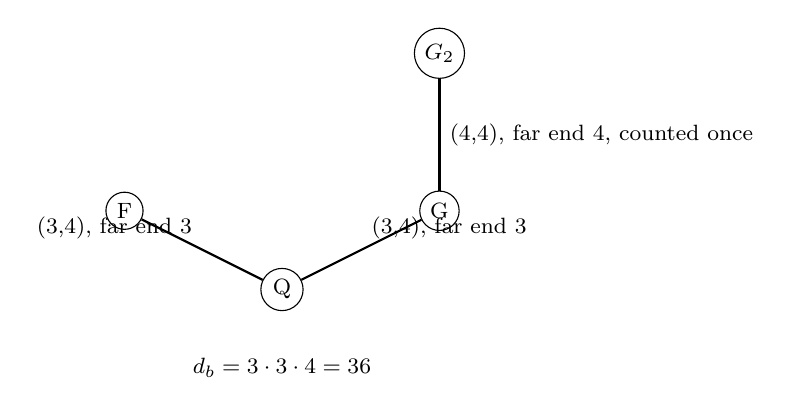
\begin{tikzpicture}[every node/.style={font=\footnotesize}]
\node[circle,draw,inner sep=2pt] (Q) at (0,0) {Q};
\node[circle,draw,inner sep=2pt] (F) at (-2,1) {F};
\node[circle,draw,inner sep=2pt] (G) at (2,1) {G};
\node[circle,draw,inner sep=2pt] (G2) at (2,3) {$G_2$};
\draw[thick] (Q) -- node[above left] {(3,4), far end 3} (F);
\draw[thick] (Q) -- node[above right] {(3,4), far end 3} (G);
\draw[thick] (G) -- node[right] {(4,4), far end 4, counted once} (G2);
\node at (0,-1) {$d_b=3\cdot 3\cdot 4=36$};
\end{tikzpicture}
\caption{The hubs and in-legs of the bottom quark body. The qutrit Q, the hubs F and G at the two (3,4) in-legs and the hub $G_2$ at the one (4,4) hub-to-hub in-leg, whose far-end dimensions multiply to the dressing thirty-six. The out-legs and docks of the body are not drawn.}
\end{figure}
\par\medskip\noindent{\itshape Mass read, Part XI turns to the Higgs.}\label{narr:close:8-5}\par
\section{The Yukawa as the (3,4)-leg office at every body}\label{mod:VI-7a-D541324-w-yklo}
\chdesig{10-6}{6-7a}{VI-7a-D541324-w-yklo}{VI-7a-D541324-w-yklo}
\begin{chwall}[The Yukawa as the (3,4)-leg office at every body]\label{box:VI-7a-D541324-w-yklo:1}
No one per-leg cell among the leg unit, the free-genre first power, the dressing base and their squares factors the offices as the vacuum register multiplied by the cell to the unpassed (3,4) in-leg count: the first parting body is the electron at the count zero at every candidate, its office over the register an element of the field with root parts against the cell one, the equal count zero of 2847 at every candidate, the chain ratios re-met at the neutron over the proton alone, nine at the exponent difference one, the dressing base squared; the top Yukawa cell of the Higgs-and-carrier-offices entry is re-met as the proton office over the register $101761/81$ with the implied per-leg cell $319/9$ at the count two, the hadron cap over the dressing base squared, a per-body cell and no one cell across the bodies; an open result of the factoring at the (3,4) legs under the axiom text, compared with nothing.
The first face, one per-leg cell at every body with the chain re-met, reads unmet; the second face, the first parting body named with both cells, reads yes at the electron, its office over the register against the cell one. Open is the Yukawa as one cell at the (3,4) legs: the top cell of the foregoing entry stands at one body, and a per-leg cell factors no other office.
\end{chwall}
\chstanding{an open result}
\chdeps{Definitions 1.1 to 1.6}{no theorem beyond it at this release}
The top Yukawa of the Higgs-and-carrier-offices entry is the office of one body over the vacuum register at the hub. The question is whether that cell generalizes: whether every office of the five bodies and the 2842 carrier bodies equals the vacuum register multiplied by one fixed per-leg cell raised to the number of (3,4) in-legs its passage leaves unpassed. Six candidates for the cell are read from the entries, the leg unit twelve, the free-genre first power twelve, the dressing base three and their squares, and the vacuum register at its six readings. The electron parts first: its passage passes its one in-leg, so its count is zero and the candidate to the zeroth power is one, while its office over the register carries root parts; at the proton the ratio is the square of $319/9$, a cell of the proton alone. No candidate meets any body, and only the neutron over the proton re-meets a chain ratio.
\begin{chbridge}
In the Standard Model the mass of each fermion is its Yukawa coupling multiplied by the vacuum expectation value of the Higgs field divided by root two, one coupling per body and no relation among them, the top coupling near unity and the others small \cite{Weinberg1967,Peskin1995}. The correspondence is by name.
\end{chbridge}
\begin{chproof}[exhaustive census with its exact part]
The premises of this derivation are the axiom and the six definitions of chapter~\ref{mod:FRAMEWORK}, the body-alone office rule of chapter~\ref{mod:VIII-2-body-alone-office-rule}, a theorem, the dressing as the unpassed (3,4) in-legs of chapter~\ref{mod:VIII-1-mass-unit-and-the-first-power}, a theorem, the Higgs and carrier offices at their sinks of chapter~\ref{mod:VI-10-higgs-the-closed-hub-read-its-rows-its-mass-and-its-exponent}, a theorem, and the vacuum register of the chapter titled The electroweak table (chapter~\ref{mod:VI-9-electroweak-table}, among the instruments), an instrument. The chain of premises runs back to the axiom through those chapters, and the longest such chain in this compendium is twelve chapters long.
\textit{The exact part.} For each body the passage is walked as the unpassed-in-legs entry walks it, the entry at the pendant qubit of the first dock-set link in link order, the stop at the first-reached hubs, every in-leg dressed at a tie and the base the far-end dimension, giving the count $k$ of unpassed (3,4) in-legs, zero at the electron, two at the muon and the proton, three at the tau sink. The six candidates $c$ are 12, 12, 3, 144, 144 and 9, and the vacuum register $R$ is 6561 at its first reading. At the proton,
\begin{equation} \frac{\Omega_{P}}{R} = \frac{101761}{81} = \Big(\frac{319}{9}\Big)^{2}, \qquad c^{2} \in \{144,\ 144,\ 9,\ 20736,\ 20736,\ 81\}, \end{equation}
so the ratio is an exact square whose root $319/9$, the hadron cap over the dressing base squared, equals none of the candidates squared, and the top Yukawa cell is re-met as a cell of the proton alone. At the electron the count is zero and every candidate to the zeroth power is one, while
\begin{equation} \frac{\Omega_{E}}{R} \ \text{carries nonzero root-two and root-three coordinates,} \qquad \frac{\Omega_{E}}{R} \neq 1 , \end{equation}
the four coordinates printed at the table of the entry, so the electron parts at every candidate and is the first parting body. The figure draws the electron web with its passed in-leg.
\textit{The census.} By exhaustive enumeration of the 2847 bodies, the five bodies and the 2842 carrier bodies, with the tau web of the library and the one-link electron web beside: each body is located and walked, 2847 of 2847, the walk re-met against the unpassed-in-legs entry at every cell of the five bodies and the tau sink and against the sinks table of the carrier-bodies entry at every cell of the 2842; the property tested at each body and candidate is whether the residual, the office over the register multiplied by the candidate to the count, is an exact element of the field and whether it equals one; the counts are the residuals exact at 17094 of 17094, the two-read identity holding at every residual, and the letter equal at zero of 2847 bodies at every candidate, the closing candidates none; the chain ratios of the mass-ratios entry are re-met as ratios of the cells at one pair and one candidate alone, the neutron over the proton at nine, the dressing base squared at the exponent difference one. The smallest case is the electron worked above.
\textit{The check.} The counter-tests alter the construction singly and read what moves. Striking the vacuum register moves every residual. Striking the passage moves the electron from the count zero. Striking the square moves the proton residual. Striking the text unmeets the gate. Striking the closure moves the electron residual with the proton and the neutron at a closure of zero unmoved. Each alteration moves the cells it names, five of five. The result was reproduced by an independent route, two engines built apart, the python route against the ruby route, equal at every cell, with the sixteen controls the same.
\chcert{2847}
\begin{figure}[h]\centering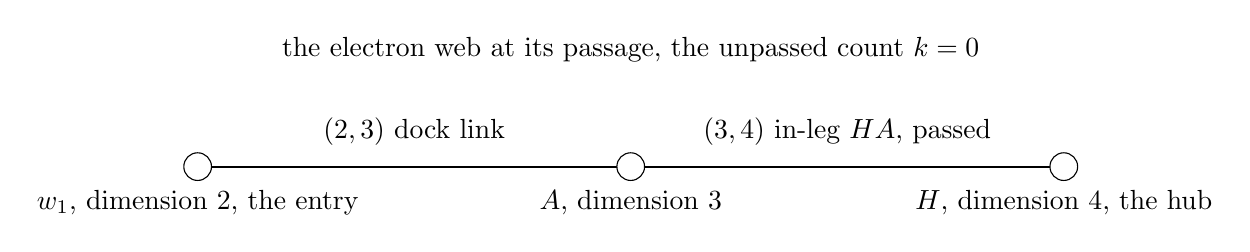
\begin{tikzpicture}[scale=1]
\draw[thick] (0,0) -- (5.5,0); \draw[thick] (5.5,0) -- (11,0);
\filldraw[fill=white] (0,0) circle (5pt) node[below=5pt] {$w_1$, dimension 2, the entry};
\filldraw[fill=white] (5.5,0) circle (5pt) node[below=5pt] {$A$, dimension 3};
\filldraw[fill=white] (11,0) circle (5pt) node[below=5pt] {$H$, dimension 4, the hub};
\node at (2.75,0) [above=4pt] {$(2,3)$ dock link}; \node at (8.25,0) [above=4pt] {$(3,4)$ in-leg $HA$, passed};
\node at (5.5,1) [above=6pt] {the electron web at its passage, the unpassed count $k = 0$};
\end{tikzpicture}\caption{The passage of the electron web: entered at the pendant qubit of its dock link, it reaches the hub through its one (3,4) in-leg, which is therefore passed, so the unpassed count is zero and the first parting stands here.}\end{figure}
\end{chproof}

\clearpage
\part*{Part XI. The Higgs, Its Hub Register And The Dressing Field\\[5pt]{\large The (4,4) cell}}
\label{atlaspart:11-cell-4-4-higgs}
\addcontentsline{toc}{part}{Part XI. The Higgs, Its Hub Register And The Dressing Field, The (4,4) cell}
This Part reads the (4,4) cell. The expectation register of the hub, the vacuum register and the horizon cut register one register by construction, is to be read as a count of the Higgs sector at a later result, and that reading is stated here as an expectation and not as a claim of this Part.
\section{The Higgs: the closed hub read, its rows, its mass and its exponent}\label{mod:VI-10-higgs-the-closed-hub-read-its-rows-its-mass-and-its-exponent}
\chdesig{11-1}{6-10}{VI-10-higgs-the-closed-hub-read-its-rows-its-mass-and-its-exponent}{VI-10-D540200-hqrt-t1}
\label{narr:open:6-10}Theorem~200.1 reads the Higgs as the closed hub read, Theorem~200.2 its port, rows and weight, Theorem~200.3 its mass, vacuum port and exponent, and Open result~200.4 the three readings of the attachment; Open result~200.5 states the attachment at the saturated web as an open result and Theorem~200.6, a theorem, gives the Higgs and carrier offices at their sinks, the cells the register matrix prints.
\begin{chconditional}[The Higgs as the closed hub read]\label{box:VI-10-higgs-the-closed-hub-read-its-rows-its-mass-and-its-exponent:1}
Under the link lemmas, the body read at the lepton and the carriers from the readable genres, the Higgs word of the roster, the (4,4) attachment at ends of one dimension, is the closed read of its hub at the adopted closure, matched at the mass face and met again at the unit and the attachment: a carrier has a mass face if and only if it is closed at the ends of its chain, at all five catalogued carriers.
\end{chconditional}
\chstanding{conditional theorem}
\chdeps{the theorems of Chapters 1-0, 1-2 to 1-4, 1-6, 5-2 to 5-3, 8-3, 10-1}{the theorems of Chapters 1-1 to 1-2, 3-1, 5-3, 5-8f, 5-13, 6-3, 11-1}
The box reads the Higgs word, one link joining two ququarts, as the read whose hub is closed at both ends, and shows that the closure at the ends of a carrier chain is exactly what the prior link lemmas called a mass face, at every one of the five carriers.
\begin{chconditional}[The port, the rows and the weight of the Higgs word]\label{box:VI-10-higgs-the-closed-hub-read-its-rows-its-mass-and-its-exponent:2}
Under their parents, the port of the Higgs word is sealed at every clause, the one (4,4) link of the word unread at every clause; its four rows are keyed at every one of the seven distinct (3,4) junction legs of the six catalogued links, the unit the far end with the first power 12; and the Yukawa weight is the first power under its hub-pair name and no new object.
\end{chconditional}
\chstanding{conditional theorems, three}
\chdeps{the theorems of Chapters 1-0, 1-2 to 1-4, 1-6, 5-2 to 5-3, 8-3, 10-1}{the theorems of Chapters 1-1 to 1-2, 3-1, 5-3, 5-8f, 5-13, 6-3, 11-1}
The second box gathers three results on the same word, its link is never read, its rows live on the junction legs that join a qutrit to a ququart, and the weight the literature would call a Yukawa coupling is the first power already defined.
\begin{chconditional}[The mass, the vacuum port and the exponent]\label{box:VI-10-higgs-the-closed-hub-read-its-rows-its-mass-and-its-exponent:3}
Under their parents, the two faces of the Higgs mass are defined as exact objects at both port faces at the order-two attachment read; the primary port at the W word is the dock, the one port reading that is an output of the definition of open at the office, its register 6561 at the dock unit 67; and the direct two-exchange sum of the Higgs word equals the first power of its closed read and not its square, so the exponent is one and the word reads at the order two and no lower.
\end{chconditional}
\chstanding{conditional theorems, three}
\chdeps{the theorems of Chapters 1-0, 1-2 to 1-4, 1-6, 5-2 to 5-3, 8-3, 10-1}{the theorems of Chapters 1-1 to 1-2, 3-1, 5-3, 5-8f, 5-13, 6-3, 11-1}
The third box gives the mass as an exact object at two faces, names the port the vacuum register is read at, and fixes the exponent of the closed read at one.
\begin{chwall}[The three readings of the attachment]\label{box:VI-10-higgs-the-closed-hub-read-its-rows-its-mass-and-its-exponent:4}
The attachment is closed at the primary pair reading with the Higgs rows keyed at none of the four; the vacuum row parts the office rule at the leg unit; and the content cell of the attachment web is the singlet against the two-factor doublet, each an open result at its named step.
\end{chwall}
\chstanding{open results, three, built and not closed}
\chdeps{the theorems of Chapters 1-0, 1-2 to 1-4, 1-6, 5-2 to 5-3, 8-3, 10-1}{the theorems of Chapters 1-1 to 1-2, 3-1, 5-3, 5-8f, 5-13, 6-3, 11-1}
The fourth box names the three readings of the attachment that are tried and parted.
\begin{chbridge}
What this chapter calls the Higgs word the literature calls the Higgs boson, its closed hub read the Higgs field at its vacuum, the first power under the hub-pair name a Yukawa coupling, the vacuum register the vacuum expectation value and the exponent the order of the self-coupling, each by name only. The correspondence is by name, and every mass figure stands at the comparison table.
\end{chbridge}
\begin{chproof}[census]
The premises are the link and its six genres of chapter 1-2, the reads and the Born count of chapter 1-3 and the moves of chapter 1-4, definitions, the read at a register of chapter 1-6, the gauge chapters 4-2 and 4-3, the doublets of chapter 6-3 and the mass unit of chapter 8-1. The chain from the axiom to this chapter is eight chapters long. The set counted is the set of cataloged carriers, five words in the catalog order, the photon word, the W word, the Z word, the gluon word and the Higgs word, generated from the catalog of 64 webs, 1334 sites, 1691 links and 233 hub lines, every link genre equal to its two site dimensions at 1691 of 1691 and every hub line re-met from the sites and links at 233 of 233. The property tested is the closure at the ends of the carrier chain, every carrier a path with two ends. By kind the ends read. The photon word open, its ends of dimensions 2 and 3. The W word closed, its ends of dimension 4 and 4. The Z word closed, 4 and 4. The gluon word closed, 3 and 3. The Higgs word closed, and a mass face at the link lemmas stands at exactly the closed carriers, 5 of 5 matching, the first differing carrier none. The smallest case is the Higgs word itself, one (4,4) link,
\begin{equation}
16 = 4 \cdot 4 ,
\end{equation}
its rank and first power, no dock, its two hubs at in one and out none, the chain of one link closed at both ends and its mass face present. The exact part. From the electron web, the rank 79 less the two (2,3) docks at 6 each, we obtain the hub unit
\begin{equation}
67 = 79 - 12, \qquad 201 = 67 \cdot 3 ,
\end{equation}
the register of the closed hub at the dock and at the hub, re-met at 6 of 6 cells and at the nine chain bodies. From the attachment forcing at the closed hubs of the three closed words, six hubs at the room 3, the fresh far end is admitted at every dimension of the alphabet on the common support and its new pair read at none, the existing far ends consistent at 6966 candidates and the fresh far end consistent at 108 of 108 with the only consistent attachment at 0 of 108.

For the second and third boxes the typings of the port are counted at the rows the results name, zero on the read side and ten on the sealed side, the port struck from the rank 16 leaving the cut chain sum zero. The rows are keyed at the seven distinct (3,4) junction legs with the unit the far end at the first power 12. The records of the Higgs port are enumerated at the two-exchange register and the direct sum compared with the first power of the closed read and with its square, equal to the first and not the second, so the exponent is one. The vacuum register at the dock port is the square of the clauses register,
\begin{equation}
6561 = 81^{2} ,
\end{equation}
at the dock unit 67.

\emph{Check.} At the other four readings of the closure, the hub lines, the ports, the unit token and the face token, the match with the mass face fails at the photon word or the W word, as the closure table prints. The engines of this chapter were rerun with their captures equal byte for byte at every piece, so no cell moved. Each result was reproduced by an independent route, two engines at every capture byte for byte, its counter-tests at their pinned letters and its controls the same at both routes.
The open face of the attachment, the office rule at the leg unit and the content cell of the attachment web stay open. The mass unit and the first power are the matter of Part X.
\chcert{5}
\end{chproof}
\label{chend:VI-10-higgs-the-closed-hub-read-its-rows-its-mass-and-its-exponent}
\subsection{The Higgs attachment at the saturated web}\label{mod:VI-10-D536188-w-hgau}
\begin{chwall}[The Higgs attachment at the saturated web]\label{box:VI-10-D536188-w-hgau:1}
The Higgs attachment stands at the catalogued saturated sinks as their (4,4) links with the register 16 and the two faces of the attachment, the hub face at 16 and the leg face at 12, met again at every sink; the self-coupling, the vacuum value and the Higgs mass are exact displays at both faces, and the sink fixes the leg face where a (3,4) leg stands at a hub of its attachment link and neither face where none stands. On the one face the register is defined at every one of the 14666 attachment links; on the other face the face fixed by the sink is exactly one at 2372 of the 10123 attachment-bearing sinks, neither at 5716 and mixed at 2035, the first parting a proton sink fixing neither, named with both cells.
\end{chwall}
\chstanding{open result, built and not closed}
\chdeps{Definitions 1.1 to 1.6 and Theorems 200.1 to 200.3 and Open result 200.4}{no theorem beyond it at this release}
The box carries the attachment of the section above to every stable web of the saturation that bears one, finds the register the same everywhere, computes the three displays at both faces, and finds that the web alone does not say which face is the right one at more than half of them.
\begin{chbridge}
What this chapter calls the attachment the literature calls the coupling of the Higgs field, its self-coupling the quartic coupling, its vacuum value the vacuum expectation value and the Higgs mass the mass of the boson, each the nearest object by the rule of the section above and by name at the figure. The correspondence is by name, and the three displays are compared at the comparison table.
\end{chbridge}
\begin{chproof}[census]
The premises are the Higgs chapter above and the framework. The chain from the axiom to this result is nine chapters long. The set counted is the set of cataloged saturated sinks, 16962 webs from four sources, 14 of the roster, 16946 of the proton saturation, one of the bound-respecting seed and one lepton, parsed and equal to the census at the sites, links and genres at 16962 of 16962. The property tested is whether the sink bears the attachment, a (4,4) link, and which face its structure fixes. By kind. 10123 sinks bear the attachment as 14666 links of the genre (4,4), the register defined at 14666 of 14666 and equal to the Higgs word at the register 16. The face fixed by the sink at the adopted reading is the leg face at 2372, the hub face at 0, neither at 5716 and mixed at 2035, the first parting in the order of the material a proton sink fixing neither. The smallest case is one attachment link with its two faces, the hub face through both factors at the first power 16 and the leg face through one factor to the qutrit at the first power 12, with the self-coupling the Born square of the attachment read over the register and the vacuum value the register over the dock-struck electron unit 67,
\begin{equation}
\frac{256}{16} = 16, \qquad \frac{144}{16} = 9, \qquad \frac{16}{67} ,
\end{equation}
at the product register of the construction, and 1, 9/16 and 256/67 at the whole register beside. The mass displays at the two faces 16 over 67 and 12 over 67.

From the two faces of the attachment unit, 16 through both factors and 12 through one factor to the qutrit, equal to the faces of the parent result, by the census of the face fixed at the three readings, we obtain at the adopted reading 0 and 2372, at the pair reading 0 and 894, and at the available reading 8439 and 0, so the face fixed by the structure the read passes through and not uniformly across the saturated web. The unit of the construction, the dock-struck electron unit $79 - 12 = 67$, is re-derived from the catalog and equals the Yukawa bodies table and the attachment-read result.

\emph{Check.} One control of this result, the count of the catalog's closing lines, read 3446 against 3382 at the pinned engines, the bare closer of each block counted as a line, and 3382 at the precheck route and at the second-release engines with every deciding cell equal. Its fallback was recorded and did not fire. The result was reproduced by an independent route, two engines at every capture byte for byte, its counter-tests at their pinned letters.
The face of the attachment is fixed by the structure of each sink and by the saturated web as a whole not.
\chcert{14666}
\end{chproof}
\label{chend:VI-10-D536188-w-hgau}
\subsection{The Higgs and carrier offices at their sinks}\label{mod:VI-10-D538733-hcos-t1}
\begin{chtheorem}[The Higgs and carrier offices at their sinks]\label{box:VI-10-D538733-hcos-t1:1}
Every Higgs and carrier office of the compendium is an exact structure by the body-alone rule at the roster words: the closed-genre objects and the free genres are read at their own sinks, every office is an exact cell at every reading the results admit, and every ratio among them is an exact rational or ring cell, at all 52 ratios; the Higgs faces close 2 of 2, the carriers 6 of 6, and no sink the rule does not close and no ratio with no second read is found.
\end{chtheorem}
\chstanding{theorem}
\chdeps{Definitions 1.1 to 1.6, Theorem 195.1 and Theorems 200.1 to 200.3 and Open result 200.4}{no theorem beyond it at this release}
The box applies one rule, the office of a body read at its own stable web, to the Higgs word at both its faces and to the four carrier reads, and forms every ratio among the offices. Every office and every ratio comes out as an exact number of the ring.
\begin{chbridge}
What this chapter calls the Higgs office the literature calls the squared Higgs mass in the unit of the construction, the carrier offices the squared boson masses, and the stiffness the quartic coupling, each the nearest object. The correspondence is by name.
\end{chbridge}
\begin{chproof}[exact]
The premises are the Higgs chapter above and the body-alone office rule of chapter 8-2, a theorem, the chain from the axiom nine chapters long. The set counted is the reads the rule admits at the roster words, the Higgs word at both faces, the W and Z words at their cataloged webs, their closed-genre reads and the two free genres at one link each, with the 52 ratios among them, and the property tested is whether the rule closes the office as an exact cell. The exact part. From the Higgs word at the hub face, the (4,4) attachment at the register 16, by the first power squared plus the closure at the one dark link under the (4,4) law, we obtain the office
\begin{equation}
16^{2} + \frac{1681}{182250000} = \frac{46656001681}{182250000} ,
\end{equation}
and at the leg face, the (3,4) piece through one factor to the qutrit at the first power 12, the office $144$ plus a root-three closure, $4299817692073/29859840000 + (5069/373248000)\sqrt{3}$. From the W word at its cataloged web, the first power 28 with two (2,4) legs dark under the slot rule, we obtain the office
\begin{equation}
28^{2} + \frac{10241}{3645000} + \frac{98}{50625}\sqrt{2} = \frac{2857690241}{3645000} + \frac{98}{50625}\sqrt{2} ,
\end{equation}
the Z word the same web and its office the same, their ratio 1. By kind the offices close at 2 of 2 Higgs faces and 6 of 6 carrier reads, and the ratios are exact at 52 of 52, every one with a second read. The smallest ratio is the stiffness, the Higgs office at the hub face over the vacuum register $6561 = 81^{2}$,
\begin{equation}
\frac{46656001681}{182250000 \cdot 6561} = \frac{46656001681}{1195742250000} .
\end{equation}
\end{chproof}
\begin{chproof}[census]
The register of the attachment equals the Higgs word at 14666 of 14666 links across 10123 sinks, the first powers re-met at the carrier-mass, vacuum, scale-body and weak-angle results, and the first parting is none at either face.

\emph{Check.} The stiffness at the acts exponent and at the hub-port register reads 46656001681 over 14762250000 and over 46656000000, the office register re-met the same, and the result was reproduced by an independent route, its four counter-tests and sixteen controls at their pinned letters.
\chcert{52}
\end{chproof}
\begin{figure}[H]\centering
\begin{tikzpicture}[x=0.52pt,y=-0.52pt,baseline]
\clip (0,0) rectangle (900,540);
\fill[white] (0,0) rectangle (900,540);
\node[anchor=base west,inner sep=0pt,text=black,font=\fontsize{6.76}{8.112}\selectfont\ttfamily] at (12,22) {atlas r-hig: r-hig};
\node[anchor=base west,inner sep=0pt,text=black,font=\fontsize{6.24}{7.488}\selectfont\ttfamily] at (12,42) {membership 22:0;23:0;24:0;33:0;34:0;44:1; cells (4,4); links 1; sites 2; measure 16; census at the census};
\node[anchor=base west,inner sep=0pt,text=black,font=\fontsize{5.72}{6.864}\selectfont\ttfamily] at (12,62) {recorded office offices:HH:measure struck/slot/in-leg-34/R1/weight:HH=46656001681/182250000\textbar{}0\textbar{}0\textbar{}0; standing census:instrument;offices:theorem;formula:open result;roster:roster word; board Higgs};
\draw[draw=black,line width=1.04pt] (100,130) .. controls (130,110) and (160,110) .. (190,130);
\node[anchor=base,inner sep=0pt,text=black,font=\fontsize{5.72}{6.864}\selectfont\ttfamily] at (145,111) {(4,4)};
\filldraw[fill={rgb,255:red,112;green,112;blue,112},draw=black,line width=0.52pt] (100,130) circle (14);
\node[anchor=base,inner sep=0pt,text=white,font=\fontsize{6.24}{7.488}\selectfont\ttfamily] at (100,135) {4};
\node[anchor=base,inner sep=0pt,text=black,font=\fontsize{5.72}{6.864}\selectfont\ttfamily] at (100,160) {s1};
\filldraw[fill={rgb,255:red,112;green,112;blue,112},draw=black,line width=0.52pt] (190,130) circle (14);
\node[anchor=base,inner sep=0pt,text=white,font=\fontsize{6.24}{7.488}\selectfont\ttfamily] at (190,135) {4};
\node[anchor=base,inner sep=0pt,text=black,font=\fontsize{5.72}{6.864}\selectfont\ttfamily] at (190,160) {s2};
\node[anchor=base west,inner sep=0pt,text=black,font=\fontsize{5.72}{6.864}\selectfont\ttfamily] at (12,510) {the sites labelled by register (2 the qubit, white; 3 the qutrit, grey; 4 the ququart, dark); the links labelled by cell (p,q); a long dash an open dark link of the neutron row; a short dash a docked link at the rule R1};
\end{tikzpicture}
\caption{\texttt{r-hig} (the Higgs), Higgs: 2 sites, 1 links, the measure 16; the links at the cells (4,4); the membership 22:0; 23:0; 24:0; 33:0; 34:0; 44:1; dock-free at the rule R1; at the census of the six cells. Drawn at the anatomy atlas as its web, the sites labeled by register and the links by cell, from the the Higgs and carrier offices at their sinks.}\label{fig:VI-10-D538733-r-hig-55890f}
\begin{center}\footnotesize\begin{adjustbox}{max width=\linewidth}\begin{tabular}{p{0.26\textwidth}p{0.68\textwidth}}\toprule
recorded office (the slot-count row) & the read o-hh of the formula row: the first power 16; the office \texttt{46656001681/182250000\textbar{}0\textbar{}0\textbar{}0}; against the formula with the slot count equal; the slot total 0; dark links 1; hubs none; dressing 1 \\
mass register (the mass-register row) & the read HH: the class touching the ququart; the first power 16; the office \texttt{46656001681/182250000\textbar{}0\textbar{}0\textbar{}0}; nonzero; met yes; hubs none; in-legs none; dressing 1; ports s1-s2 \\
\bottomrule\end{tabular}\end{adjustbox}\end{center}
\end{figure}
\begin{figure}[H]\centering
\begin{tikzpicture}[x=0.52pt,y=-0.52pt,baseline]
\clip (0,0) rectangle (900,540);
\fill[white] (0,0) rectangle (900,540);
\node[anchor=base west,inner sep=0pt,text=black,font=\fontsize{6.76}{8.112}\selectfont\ttfamily] at (12,22) {atlas offices:F34: free-genre-(3,4)};
\node[anchor=base west,inner sep=0pt,text=black,font=\fontsize{6.24}{7.488}\selectfont\ttfamily] at (12,42) {membership 22:0;23:0;24:0;33:0;34:1;44:0; cells (3,4); links 1; sites 2; measure 12; census at the census};
\node[anchor=base west,inner sep=0pt,text=black,font=\fontsize{5.72}{6.864}\selectfont\ttfamily] at (12,62) {recorded office offices:F34:measure struck/slot/in-leg-34/R1/weight:F34=4299817692073/29859840000\textbar{}0\textbar{}5069/373248000\textbar{}0; standing census:instrument;offices:theorem;formula:open result; board none};
\draw[draw=black,line width=1.04pt] (100,470) .. controls (130,450) and (160,450) .. (190,470);
\node[anchor=base,inner sep=0pt,text=black,font=\fontsize{5.72}{6.864}\selectfont\ttfamily] at (145,451) {(3,4)};
\filldraw[fill={rgb,255:red,244;green,192;blue,192},draw=black,line width=0.52pt] (100,470) circle (14);
\node[anchor=base,inner sep=0pt,text=black,font=\fontsize{6.24}{7.488}\selectfont\ttfamily] at (100,475) {0};
\node[anchor=base,inner sep=0pt,text=black,font=\fontsize{5.72}{6.864}\selectfont\ttfamily] at (100,500) {x3};
\filldraw[fill={rgb,255:red,244;green,192;blue,192},draw=black,line width=0.52pt] (190,470) circle (14);
\node[anchor=base,inner sep=0pt,text=black,font=\fontsize{6.24}{7.488}\selectfont\ttfamily] at (190,475) {0};
\node[anchor=base,inner sep=0pt,text=black,font=\fontsize{5.72}{6.864}\selectfont\ttfamily] at (190,500) {y4};
\node[anchor=base west,inner sep=0pt,text=black,font=\fontsize{5.72}{6.864}\selectfont\ttfamily] at (12,510) {the sites labelled by register (2 the qubit, white; 3 the qutrit, grey; 4 the ququart, dark); the links labelled by cell (p,q); a long dash an open dark link of the neutron row; a short dash a docked link at the rule R1};
\end{tikzpicture}
\caption{\texttt{free-genre-(3,4)}, free: 2 sites, 1 links, the measure 12; the links at the cells (3,4); the membership 22:0; 23:0; 24:0; 33:0; 34:1; 44:0; dock-free at the rule R1; at the census of the six cells; 2 sites at the fourth band with the register unresolved by the genre alone, the drawing gloss not drawn at them as the compendium prints it. Drawn at the anatomy atlas as its web, the sites labeled by register and the links by cell, from the the Higgs and carrier offices at their sinks.}\label{fig:VI-10-D538733-free-genre-3-4-131d45}
\begin{center}\footnotesize\begin{adjustbox}{max width=\linewidth}\begin{tabular}{p{0.26\textwidth}p{0.68\textwidth}}\toprule
recorded office (the slot-count row) & the read O-F34 of the formula row: the first power 12; the office \texttt{4299817692073/29859840000\textbar{}0\textbar{}5069/373248000\textbar{}0}; against the formula with the slot count equal; the slot total 0; dark links 1; hubs none; dressing 1 \\
mass register (the mass-register row) & the read F34: the class touching the ququart; the first power 12; the office \texttt{4299817692073/29859840000\textbar{}0\textbar{}5069/373248000\textbar{}0}; nonzero; met yes; hubs none; in-legs none; dressing 1; ports x3-y4 \\
\bottomrule\end{tabular}\end{adjustbox}\end{center}
\end{figure}
\begin{figure}[H]\centering
\begin{tikzpicture}[x=0.52pt,y=-0.52pt,baseline]
\clip (0,0) rectangle (900,540);
\fill[white] (0,0) rectangle (900,540);
\node[anchor=base west,inner sep=0pt,text=black,font=\fontsize{6.76}{8.112}\selectfont\ttfamily] at (12,22) {atlas offices:HL: leg-piece-(3,4)};
\node[anchor=base west,inner sep=0pt,text=black,font=\fontsize{6.24}{7.488}\selectfont\ttfamily] at (12,42) {membership 22:0;23:0;24:0;33:0;34:1;44:0; cells (3,4); links 1; sites 2; measure 12; census at the census};
\node[anchor=base west,inner sep=0pt,text=black,font=\fontsize{5.72}{6.864}\selectfont\ttfamily] at (12,62) {recorded office offices:HL:measure struck/slot/in-leg-34/R1/weight:HL=4299817692073/29859840000\textbar{}0\textbar{}5069/373248000\textbar{}0; standing census:instrument;offices:theorem;formula:open result; board none};
\draw[draw=black,line width=1.04pt] (100,470) .. controls (130,450) and (160,450) .. (190,470);
\node[anchor=base,inner sep=0pt,text=black,font=\fontsize{5.72}{6.864}\selectfont\ttfamily] at (145,451) {(3,4)};
\filldraw[fill={rgb,255:red,244;green,192;blue,192},draw=black,line width=0.52pt] (100,470) circle (14);
\node[anchor=base,inner sep=0pt,text=black,font=\fontsize{6.24}{7.488}\selectfont\ttfamily] at (100,475) {0};
\node[anchor=base,inner sep=0pt,text=black,font=\fontsize{5.72}{6.864}\selectfont\ttfamily] at (100,500) {h};
\filldraw[fill={rgb,255:red,244;green,192;blue,192},draw=black,line width=0.52pt] (190,470) circle (14);
\node[anchor=base,inner sep=0pt,text=black,font=\fontsize{6.24}{7.488}\selectfont\ttfamily] at (190,475) {0};
\node[anchor=base,inner sep=0pt,text=black,font=\fontsize{5.72}{6.864}\selectfont\ttfamily] at (190,500) {q};
\node[anchor=base west,inner sep=0pt,text=black,font=\fontsize{5.72}{6.864}\selectfont\ttfamily] at (12,510) {the sites labelled by register (2 the qubit, white; 3 the qutrit, grey; 4 the ququart, dark); the links labelled by cell (p,q); a long dash an open dark link of the neutron row; a short dash a docked link at the rule R1};
\end{tikzpicture}
\caption{\texttt{leg-piece-(3,4)}, Higgs: 2 sites, 1 links, the measure 12; the links at the cells (3,4); the membership 22:0; 23:0; 24:0; 33:0; 34:1; 44:0; dock-free at the rule R1; at the census of the six cells; 2 sites at the fourth band with the register unresolved by the genre alone, the drawing gloss not drawn at them as the compendium prints it. Drawn at the anatomy atlas as its web, the sites labeled by register and the links by cell, from the the Higgs and carrier offices at their sinks.}\label{fig:VI-10-D538733-leg-piece-3-4-5a3770}
\begin{center}\footnotesize\begin{adjustbox}{max width=\linewidth}\begin{tabular}{p{0.26\textwidth}p{0.68\textwidth}}\toprule
recorded office (the slot-count row) & the read o-hl of the formula row: the first power 12; the office \texttt{4299817692073/29859840000\textbar{}0\textbar{}5069/373248000\textbar{}0}; against the formula with the slot count equal; the slot total 0; dark links 1; hubs none; dressing 1 \\
mass register (the mass-register row) & the read HL: the class touching the ququart; the first power 12; the office \texttt{4299817692073/29859840000\textbar{}0\textbar{}5069/373248000\textbar{}0}; nonzero; met yes; hubs none; in-legs none; dressing 1; ports h-q \\
\bottomrule\end{tabular}\end{adjustbox}\end{center}
\end{figure}
\begin{figure}[H]\centering
\begin{tikzpicture}[x=0.52pt,y=-0.52pt,baseline]
\clip (0,0) rectangle (900,540);
\fill[white] (0,0) rectangle (900,540);
\node[anchor=base west,inner sep=0pt,text=black,font=\fontsize{6.76}{8.112}\selectfont\ttfamily] at (12,22) {atlas offices:F24: free-genre-(2,4)};
\node[anchor=base west,inner sep=0pt,text=black,font=\fontsize{6.24}{7.488}\selectfont\ttfamily] at (12,42) {membership 22:0;23:0;24:1;33:0;34:0;44:0; cells (2,4); links 1; sites 2; measure 8; census at the census};
\node[anchor=base west,inner sep=0pt,text=black,font=\fontsize{5.72}{6.864}\selectfont\ttfamily] at (12,62) {recorded office offices:F24:measure struck/slot/in-leg-34/R1/weight:F24=466566137/7290000\textbar{}2/6075\textbar{}0\textbar{}0; standing census:instrument;offices:theorem;formula:open result; board none};
\draw[draw=black,line width=1.04pt] (100,470) .. controls (130,450) and (160,450) .. (190,470);
\node[anchor=base,inner sep=0pt,text=black,font=\fontsize{5.72}{6.864}\selectfont\ttfamily] at (145,451) {(2,4)};
\filldraw[fill={rgb,255:red,244;green,192;blue,192},draw=black,line width=0.52pt] (100,470) circle (14);
\node[anchor=base,inner sep=0pt,text=black,font=\fontsize{6.24}{7.488}\selectfont\ttfamily] at (100,475) {0};
\node[anchor=base,inner sep=0pt,text=black,font=\fontsize{5.72}{6.864}\selectfont\ttfamily] at (100,500) {x2};
\filldraw[fill={rgb,255:red,244;green,192;blue,192},draw=black,line width=0.52pt] (190,470) circle (14);
\node[anchor=base,inner sep=0pt,text=black,font=\fontsize{6.24}{7.488}\selectfont\ttfamily] at (190,475) {0};
\node[anchor=base,inner sep=0pt,text=black,font=\fontsize{5.72}{6.864}\selectfont\ttfamily] at (190,500) {y4};
\node[anchor=base west,inner sep=0pt,text=black,font=\fontsize{5.72}{6.864}\selectfont\ttfamily] at (12,510) {the sites labelled by register (2 the qubit, white; 3 the qutrit, grey; 4 the ququart, dark); the links labelled by cell (p,q); a long dash an open dark link of the neutron row; a short dash a docked link at the rule R1};
\end{tikzpicture}
\caption{\texttt{free-genre-(2,4)}, free: 2 sites, 1 links, the measure 8; the links at the cells (2,4); the membership 22:0; 23:0; 24:1; 33:0; 34:0; 44:0; dock-free at the rule R1; at the census of the six cells; 2 sites at the fourth band with the register unresolved by the genre alone, the drawing gloss not drawn at them as the compendium prints it. Drawn at the anatomy atlas as its web, the sites labeled by register and the links by cell, from the the Higgs and carrier offices at their sinks.}\label{fig:VI-10-D538733-free-genre-2-4-e1956c}
\begin{center}\footnotesize\begin{adjustbox}{max width=\linewidth}\begin{tabular}{p{0.26\textwidth}p{0.68\textwidth}}\toprule
recorded office (the slot-count row) & the read O-F24 of the formula row: the first power 8; the office \texttt{466566137/7290000\textbar{}2/6075\textbar{}0\textbar{}0}; against the formula with the slot count equal; the slot total 0; dark links 1; hubs none; dressing 1 \\
mass register (the mass-register row) & the read F24: the class touching the ququart; the first power 8; the office \texttt{466566137/7290000\textbar{}2/6075\textbar{}0\textbar{}0}; nonzero; met yes; hubs none; in-legs none; dressing 1; ports x2-y4 \\
\bottomrule\end{tabular}\end{adjustbox}\end{center}
\end{figure}
\begin{figure}[H]\centering
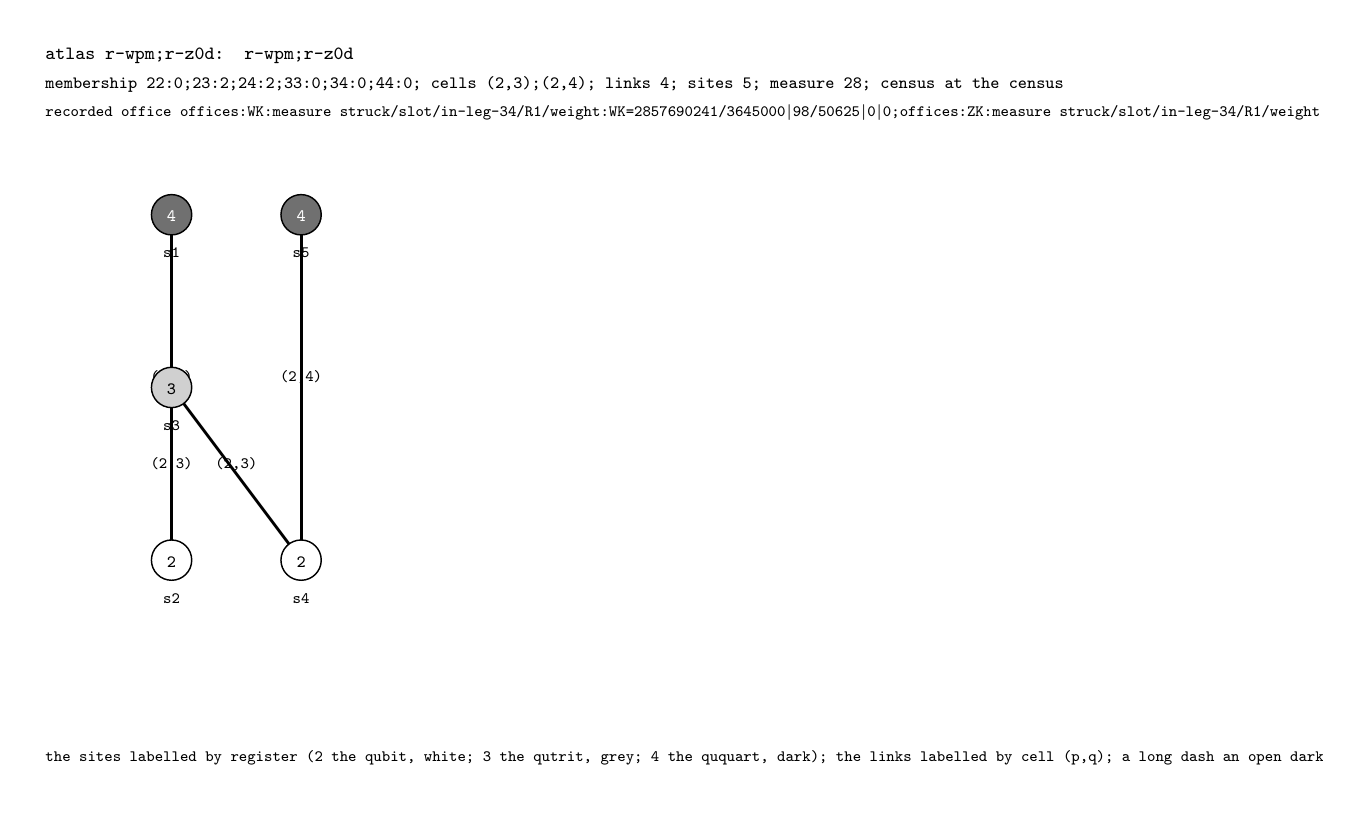
\begin{tikzpicture}[x=0.52pt,y=-0.52pt,baseline]
\clip (0,0) rectangle (900,540);
\fill[white] (0,0) rectangle (900,540);
\node[anchor=base west,inner sep=0pt,text=black,font=\fontsize{6.76}{8.112}\selectfont\ttfamily] at (12,22) {atlas r-wpm;r-z0d: r-wpm;r-z0d};
\node[anchor=base west,inner sep=0pt,text=black,font=\fontsize{6.24}{7.488}\selectfont\ttfamily] at (12,42) {membership 22:0;23:2;24:2;33:0;34:0;44:0; cells (2,3);(2,4); links 4; sites 5; measure 28; census at the census};
\node[anchor=base west,inner sep=0pt,text=black,font=\fontsize{5.72}{6.864}\selectfont\ttfamily] at (12,62) {recorded office offices:WK:measure struck/slot/in-leg-34/R1/weight:WK=2857690241/3645000\textbar{}98/50625\textbar{}0\textbar{}0;offices:ZK:measure struck/slot/in-leg-34/R1/weight:ZK=2857690241/3645000\textbar{}98/50625\textbar{}0\textbar{}0; standing census:instrument;offices:theorem;formula:open result;roster:roster word; board W};
\draw[draw=black,line width=1.04pt] (100,130) -- (100,370);
\node[anchor=base,inner sep=0pt,text=black,font=\fontsize{5.72}{6.864}\selectfont\ttfamily] at (100,246) {(2,4)};
\draw[draw=black,line width=1.04pt] (100,370) -- (100,250);
\node[anchor=base,inner sep=0pt,text=black,font=\fontsize{5.72}{6.864}\selectfont\ttfamily] at (100,306) {(2,3)};
\draw[draw=black,line width=1.04pt] (100,250) -- (190,370);
\node[anchor=base,inner sep=0pt,text=black,font=\fontsize{5.72}{6.864}\selectfont\ttfamily] at (145,306) {(2,3)};
\draw[draw=black,line width=1.04pt] (190,370) -- (190,130);
\node[anchor=base,inner sep=0pt,text=black,font=\fontsize{5.72}{6.864}\selectfont\ttfamily] at (190,246) {(2,4)};
\filldraw[fill={rgb,255:red,112;green,112;blue,112},draw=black,line width=0.52pt] (100,130) circle (14);
\node[anchor=base,inner sep=0pt,text=white,font=\fontsize{6.24}{7.488}\selectfont\ttfamily] at (100,135) {4};
\node[anchor=base,inner sep=0pt,text=black,font=\fontsize{5.72}{6.864}\selectfont\ttfamily] at (100,160) {s1};
\filldraw[fill=white,draw=black,line width=0.52pt] (100,370) circle (14);
\node[anchor=base,inner sep=0pt,text=black,font=\fontsize{6.24}{7.488}\selectfont\ttfamily] at (100,375) {2};
\node[anchor=base,inner sep=0pt,text=black,font=\fontsize{5.72}{6.864}\selectfont\ttfamily] at (100,400) {s2};
\filldraw[fill={rgb,255:red,208;green,208;blue,208},draw=black,line width=0.52pt] (100,250) circle (14);
\node[anchor=base,inner sep=0pt,text=black,font=\fontsize{6.24}{7.488}\selectfont\ttfamily] at (100,255) {3};
\node[anchor=base,inner sep=0pt,text=black,font=\fontsize{5.72}{6.864}\selectfont\ttfamily] at (100,280) {s3};
\filldraw[fill=white,draw=black,line width=0.52pt] (190,370) circle (14);
\node[anchor=base,inner sep=0pt,text=black,font=\fontsize{6.24}{7.488}\selectfont\ttfamily] at (190,375) {2};
\node[anchor=base,inner sep=0pt,text=black,font=\fontsize{5.72}{6.864}\selectfont\ttfamily] at (190,400) {s4};
\filldraw[fill={rgb,255:red,112;green,112;blue,112},draw=black,line width=0.52pt] (190,130) circle (14);
\node[anchor=base,inner sep=0pt,text=white,font=\fontsize{6.24}{7.488}\selectfont\ttfamily] at (190,135) {4};
\node[anchor=base,inner sep=0pt,text=black,font=\fontsize{5.72}{6.864}\selectfont\ttfamily] at (190,160) {s5};
\node[anchor=base west,inner sep=0pt,text=black,font=\fontsize{5.72}{6.864}\selectfont\ttfamily] at (12,510) {the sites labelled by register (2 the qubit, white; 3 the qutrit, grey; 4 the ququart, dark); the links labelled by cell (p,q); a long dash an open dark link of the neutron row; a short dash a docked link at the rule R1};
\end{tikzpicture}
\caption{\texttt{r-wpm; r-z0d} (the W word), carrier: 5 sites, 4 links, the measure 28; the links at the cells (2,3), (2,4); the membership 22:0; 23:2; 24:2; 33:0; 34:0; 44:0; dock-free at the rule R1; at the census of the six cells. Drawn at the anatomy atlas as its web, the sites labeled by register and the links by cell, from the the Higgs and carrier offices at their sinks.}\label{fig:VI-10-D538733-r-wpm-d8dad0}
\begin{center}\footnotesize\begin{adjustbox}{max width=\linewidth}\begin{tabular}{p{0.26\textwidth}p{0.68\textwidth}}\toprule
recorded office (the slot-count row) & the read o-wk of the formula row: the first power 28; the office \texttt{2857690241/3645000\textbar{}98/50625\textbar{}0\textbar{}0}; against the formula with the slot count equal; the slot total 2; dark links 2; hubs none; dressing 1 \\
mass register (the mass-register row) & the read WK: the class touching the ququart; the first power 28; the office \texttt{2857690241/3645000\textbar{}98/50625\textbar{}0\textbar{}0}; nonzero; met yes; hubs none; in-legs none; dressing 1; ports s1-s2; s4-s5 \\
\bottomrule\end{tabular}\end{adjustbox}\end{center}
\end{figure}
\begin{figure}[H]\centering
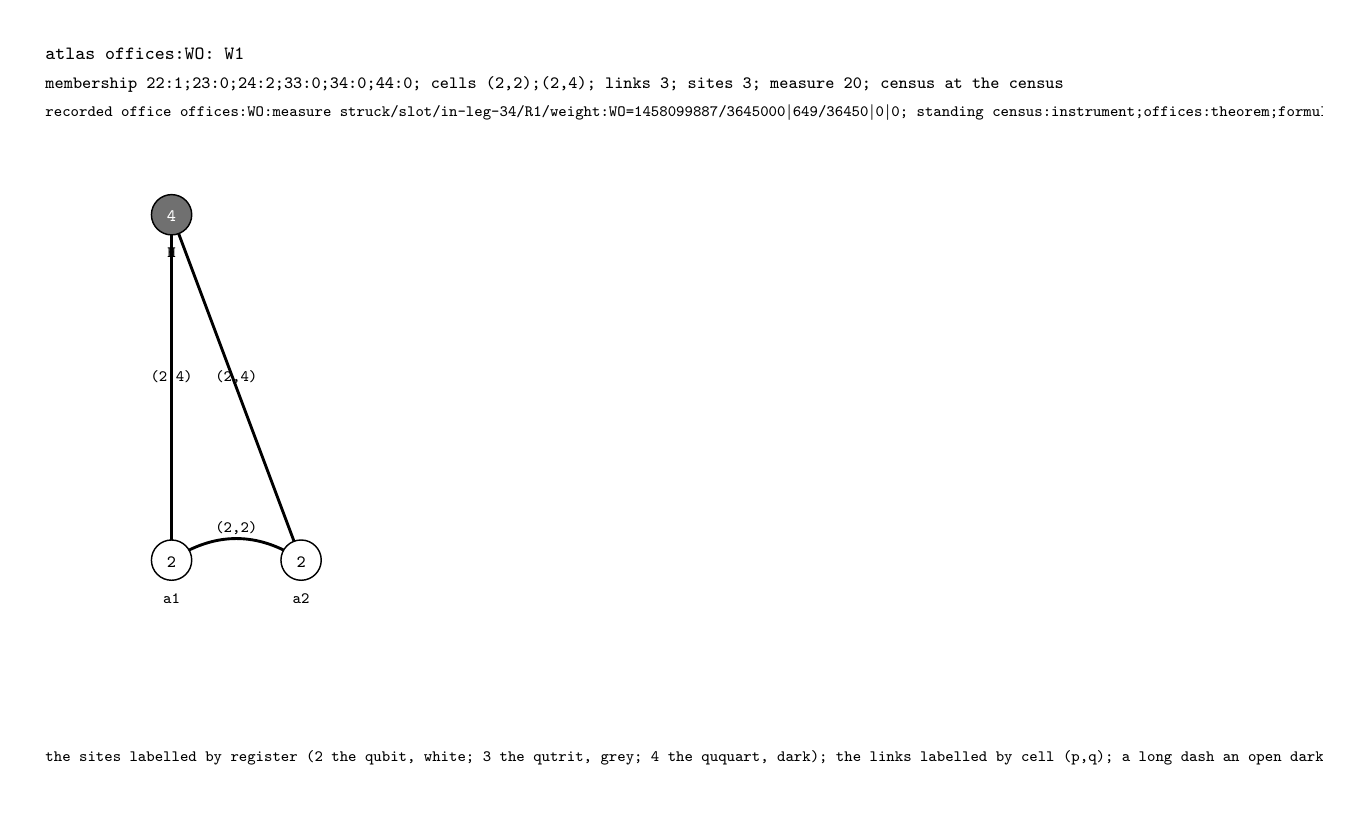
\begin{tikzpicture}[x=0.52pt,y=-0.52pt,baseline]
\clip (0,0) rectangle (900,540);
\fill[white] (0,0) rectangle (900,540);
\node[anchor=base west,inner sep=0pt,text=black,font=\fontsize{6.76}{8.112}\selectfont\ttfamily] at (12,22) {atlas offices:WO: W1};
\node[anchor=base west,inner sep=0pt,text=black,font=\fontsize{6.24}{7.488}\selectfont\ttfamily] at (12,42) {membership 22:1;23:0;24:2;33:0;34:0;44:0; cells (2,2);(2,4); links 3; sites 3; measure 20; census at the census};
\node[anchor=base west,inner sep=0pt,text=black,font=\fontsize{5.72}{6.864}\selectfont\ttfamily] at (12,62) {recorded office offices:WO:measure struck/slot/in-leg-34/R1/weight:WO=1458099887/3645000\textbar{}649/36450\textbar{}0\textbar{}0; standing census:instrument;offices:theorem;formula:open result; board none};
\draw[draw=black,line width=1.04pt] (100,130) -- (100,370);
\node[anchor=base,inner sep=0pt,text=black,font=\fontsize{5.72}{6.864}\selectfont\ttfamily] at (100,246) {(2,4)};
\draw[draw=black,line width=1.04pt] (100,130) -- (190,370);
\node[anchor=base,inner sep=0pt,text=black,font=\fontsize{5.72}{6.864}\selectfont\ttfamily] at (145,246) {(2,4)};
\draw[draw=black,line width=1.04pt] (100,370) .. controls (130,350) and (160,350) .. (190,370);
\node[anchor=base,inner sep=0pt,text=black,font=\fontsize{5.72}{6.864}\selectfont\ttfamily] at (145,351) {(2,2)};
\filldraw[fill={rgb,255:red,112;green,112;blue,112},draw=black,line width=0.52pt] (100,130) circle (14);
\node[anchor=base,inner sep=0pt,text=white,font=\fontsize{6.24}{7.488}\selectfont\ttfamily] at (100,135) {4};
\node[anchor=base,inner sep=0pt,text=black,font=\fontsize{5.72}{6.864}\selectfont\ttfamily] at (100,160) {H};
\filldraw[fill=white,draw=black,line width=0.52pt] (100,370) circle (14);
\node[anchor=base,inner sep=0pt,text=black,font=\fontsize{6.24}{7.488}\selectfont\ttfamily] at (100,375) {2};
\node[anchor=base,inner sep=0pt,text=black,font=\fontsize{5.72}{6.864}\selectfont\ttfamily] at (100,400) {a1};
\filldraw[fill=white,draw=black,line width=0.52pt] (190,370) circle (14);
\node[anchor=base,inner sep=0pt,text=black,font=\fontsize{6.24}{7.488}\selectfont\ttfamily] at (190,375) {2};
\node[anchor=base,inner sep=0pt,text=black,font=\fontsize{5.72}{6.864}\selectfont\ttfamily] at (190,400) {a2};
\node[anchor=base west,inner sep=0pt,text=black,font=\fontsize{5.72}{6.864}\selectfont\ttfamily] at (12,510) {the sites labelled by register (2 the qubit, white; 3 the qutrit, grey; 4 the ququart, dark); the links labelled by cell (p,q); a long dash an open dark link of the neutron row; a short dash a docked link at the rule R1};
\end{tikzpicture}
\caption{\texttt{W1}, carrier: 3 sites, 3 links, the measure 20; the links at the cells (2,2), (2,4); the membership 22:1; 23:0; 24:2; 33:0; 34:0; 44:0; dock-free at the rule R1; at the census of the six cells. Drawn at the anatomy atlas as its web, the sites labeled by register and the links by cell, from the the Higgs and carrier offices at their sinks.}\label{fig:VI-10-D538733-w1-e857e4}
\begin{center}\footnotesize\begin{adjustbox}{max width=\linewidth}\begin{tabular}{p{0.26\textwidth}p{0.68\textwidth}}\toprule
recorded office (the slot-count row) & the read o-wo of the formula row: the first power 20; the office \texttt{1458099887/3645000\textbar{}649/36450\textbar{}0\textbar{}0}; against the formula with the slot count equal; the slot total 0; dark links 3; hubs none; dressing 1 \\
mass register (the mass-register row) & the read WO: the class touching the ququart; the first power 20; the office \texttt{1458099887/3645000\textbar{}649/36450\textbar{}0\textbar{}0}; nonzero; met yes; hubs none; in-legs none; dressing 1; ports none \\
\bottomrule\end{tabular}\end{adjustbox}\end{center}
\end{figure}
\begin{figure}[H]\centering
\begin{tikzpicture}[x=0.52pt,y=-0.52pt,baseline]
\clip (0,0) rectangle (900,540);
\fill[white] (0,0) rectangle (900,540);
\node[anchor=base west,inner sep=0pt,text=black,font=\fontsize{6.76}{8.112}\selectfont\ttfamily] at (12,22) {atlas offices:ZO: Z1};
\node[anchor=base west,inner sep=0pt,text=black,font=\fontsize{6.24}{7.488}\selectfont\ttfamily] at (12,42) {membership 22:1;23:1;24:1;33:0;34:1;44:0; cells (2,2);(2,3);(2,4);(3,4); links 4; sites 4; measure 30; census at the census};
\node[anchor=base west,inner sep=0pt,text=black,font=\fontsize{5.72}{6.864}\selectfont\ttfamily] at (12,62) {recorded office offices:ZO:measure struck/slot/in-leg-34/R1/weight:ZO=358328664923/398131200\textbar{}637/36450\textbar{}5069/373248000\textbar{}0; standing census:instrument;offices:theorem;formula:open result; board none};
\draw[draw=black,line width=1.04pt] (100,130) -- (100,250);
\node[anchor=base,inner sep=0pt,text=black,font=\fontsize{5.72}{6.864}\selectfont\ttfamily] at (100,186) {(3,4)};
\draw[draw=black,line width=1.04pt] (100,130) -- (190,370);
\node[anchor=base,inner sep=0pt,text=black,font=\fontsize{5.72}{6.864}\selectfont\ttfamily] at (145,246) {(2,4)};
\draw[draw=black,line width=1.04pt] (100,250) -- (100,370);
\node[anchor=base,inner sep=0pt,text=black,font=\fontsize{5.72}{6.864}\selectfont\ttfamily] at (100,306) {(2,3)};
\draw[draw=black,line width=1.04pt] (100,370) .. controls (130,350) and (160,350) .. (190,370);
\node[anchor=base,inner sep=0pt,text=black,font=\fontsize{5.72}{6.864}\selectfont\ttfamily] at (145,351) {(2,2)};
\filldraw[fill={rgb,255:red,112;green,112;blue,112},draw=black,line width=0.52pt] (100,130) circle (14);
\node[anchor=base,inner sep=0pt,text=white,font=\fontsize{6.24}{7.488}\selectfont\ttfamily] at (100,135) {4};
\node[anchor=base,inner sep=0pt,text=black,font=\fontsize{5.72}{6.864}\selectfont\ttfamily] at (100,160) {H};
\filldraw[fill={rgb,255:red,208;green,208;blue,208},draw=black,line width=0.52pt] (100,250) circle (14);
\node[anchor=base,inner sep=0pt,text=black,font=\fontsize{6.24}{7.488}\selectfont\ttfamily] at (100,255) {3};
\node[anchor=base,inner sep=0pt,text=black,font=\fontsize{5.72}{6.864}\selectfont\ttfamily] at (100,280) {Q};
\filldraw[fill=white,draw=black,line width=0.52pt] (100,370) circle (14);
\node[anchor=base,inner sep=0pt,text=black,font=\fontsize{6.24}{7.488}\selectfont\ttfamily] at (100,375) {2};
\node[anchor=base,inner sep=0pt,text=black,font=\fontsize{5.72}{6.864}\selectfont\ttfamily] at (100,400) {a};
\filldraw[fill=white,draw=black,line width=0.52pt] (190,370) circle (14);
\node[anchor=base,inner sep=0pt,text=black,font=\fontsize{6.24}{7.488}\selectfont\ttfamily] at (190,375) {2};
\node[anchor=base,inner sep=0pt,text=black,font=\fontsize{5.72}{6.864}\selectfont\ttfamily] at (190,400) {b};
\node[anchor=base west,inner sep=0pt,text=black,font=\fontsize{5.72}{6.864}\selectfont\ttfamily] at (12,510) {the sites labelled by register (2 the qubit, white; 3 the qutrit, grey; 4 the ququart, dark); the links labelled by cell (p,q); a long dash an open dark link of the neutron row; a short dash a docked link at the rule R1};
\end{tikzpicture}
\caption{\texttt{Z1}, carrier: 4 sites, 4 links, the measure 30; the links at the cells (2,2), (2,3), (2,4), (3,4); the membership 22:1; 23:1; 24:1; 33:0; 34:1; 44:0; dock-free at the rule R1; at the census of the six cells. Drawn at the anatomy atlas as its web, the sites labeled by register and the links by cell, from the the Higgs and carrier offices at their sinks.}\label{fig:VI-10-D538733-z1-787243}
\begin{center}\footnotesize\begin{adjustbox}{max width=\linewidth}\begin{tabular}{p{0.26\textwidth}p{0.68\textwidth}}\toprule
recorded office (the slot-count row) & the read o-zo of the formula row: the first power 30; the office \texttt{358328664923/398131200\textbar{}637/36450\textbar{}5069/373248000\textbar{}0}; against the formula with the slot count equal; the slot total 0; dark links 3; hubs none; dressing 1 \\
mass register (the mass-register row) & the read ZO: the class touching the ququart; the first power 30; the office \texttt{358328664923/398131200\textbar{}637/36450\textbar{}5069/373248000\textbar{}0}; nonzero; met yes; hubs none; in-legs none; dressing 1; ports none \\
\bottomrule\end{tabular}\end{adjustbox}\end{center}
\end{figure}
\begin{figure}[H]\centering
\begin{tikzpicture}[x=0.52pt,y=-0.52pt,baseline]
\clip (0,0) rectangle (900,540);
\fill[white] (0,0) rectangle (900,540);
\node[anchor=base west,inner sep=0pt,text=black,font=\fontsize{6.76}{8.112}\selectfont\ttfamily] at (12,22) {atlas ta\_docked: ta\_docked};
\node[anchor=base west,inner sep=0pt,text=black,font=\fontsize{6.24}{7.488}\selectfont\ttfamily] at (12,42) {membership 22:2;23:1;24:5;33:0;34:1;44:1; cells (2,2);(2,3);(2,4);(3,4);(4,4); links 10; sites 9; measure 82; census at the census};
\node[anchor=base west,inner sep=0pt,text=black,font=\fontsize{5.72}{6.864}\selectfont\ttfamily] at (12,62) {recorded office none; standing census:instrument;hadron:open result;offices:theorem;quark:open result;roster:roster word; board none};
\draw[draw=black,line width=1.04pt] (100,130) .. controls (130,110) and (160,110) .. (190,130);
\node[anchor=base,inner sep=0pt,text=black,font=\fontsize{5.72}{6.864}\selectfont\ttfamily] at (145,111) {(4,4)};
\draw[draw=black,line width=1.04pt] (100,130) -- (100,250);
\node[anchor=base,inner sep=0pt,text=black,font=\fontsize{5.72}{6.864}\selectfont\ttfamily] at (100,186) {(3,4)};
\draw[draw=black,line width=1.04pt] (100,130) -- (190,370);
\node[anchor=base,inner sep=0pt,text=black,font=\fontsize{5.72}{6.864}\selectfont\ttfamily] at (145,246) {(2,4)};
\draw[draw=black,line width=1.04pt] (100,130) -- (280,370);
\node[anchor=base,inner sep=0pt,text=black,font=\fontsize{5.72}{6.864}\selectfont\ttfamily] at (190,246) {(2,4)};
\draw[draw=black,line width=1.04pt] (190,130) -- (370,370);
\node[anchor=base,inner sep=0pt,text=black,font=\fontsize{5.72}{6.864}\selectfont\ttfamily] at (280,246) {(2,4)};
\draw[draw=black,line width=1.04pt] (190,130) -- (460,370);
\node[anchor=base,inner sep=0pt,text=black,font=\fontsize{5.72}{6.864}\selectfont\ttfamily] at (325,246) {(2,4)};
\draw[draw=black,line width=1.04pt] (190,130) -- (550,370);
\node[anchor=base,inner sep=0pt,text=black,font=\fontsize{5.72}{6.864}\selectfont\ttfamily] at (370,246) {(2,4)};
\draw[draw=black,line width=1.04pt,dash pattern=on 1.04pt off 1.56pt] (100,370) -- (100,250);
\node[anchor=base,inner sep=0pt,text=black,font=\fontsize{5.72}{6.864}\selectfont\ttfamily] at (100,306) {(2,3)};
\draw[draw=black,line width=1.04pt] (190,370) .. controls (220,350) and (250,350) .. (280,370);
\node[anchor=base,inner sep=0pt,text=black,font=\fontsize{5.72}{6.864}\selectfont\ttfamily] at (235,351) {(2,2)};
\draw[draw=black,line width=1.04pt] (460,370) .. controls (490,350) and (520,350) .. (550,370);
\node[anchor=base,inner sep=0pt,text=black,font=\fontsize{5.72}{6.864}\selectfont\ttfamily] at (505,351) {(2,2)};
\filldraw[fill={rgb,255:red,112;green,112;blue,112},draw=black,line width=0.52pt] (100,130) circle (14);
\node[anchor=base,inner sep=0pt,text=white,font=\fontsize{6.24}{7.488}\selectfont\ttfamily] at (100,135) {4};
\node[anchor=base,inner sep=0pt,text=black,font=\fontsize{5.72}{6.864}\selectfont\ttfamily] at (100,160) {H};
\filldraw[fill={rgb,255:red,112;green,112;blue,112},draw=black,line width=0.52pt] (190,130) circle (14);
\node[anchor=base,inner sep=0pt,text=white,font=\fontsize{6.24}{7.488}\selectfont\ttfamily] at (190,135) {4};
\node[anchor=base,inner sep=0pt,text=black,font=\fontsize{5.72}{6.864}\selectfont\ttfamily] at (190,160) {H2};
\filldraw[fill=white,draw=black,line width=0.52pt] (100,370) circle (14);
\node[anchor=base,inner sep=0pt,text=black,font=\fontsize{6.24}{7.488}\selectfont\ttfamily] at (100,375) {2};
\node[anchor=base,inner sep=0pt,text=black,font=\fontsize{5.72}{6.864}\selectfont\ttfamily] at (100,400) {Jd};
\filldraw[fill={rgb,255:red,208;green,208;blue,208},draw=black,line width=0.52pt] (100,250) circle (14);
\node[anchor=base,inner sep=0pt,text=black,font=\fontsize{6.24}{7.488}\selectfont\ttfamily] at (100,255) {3};
\node[anchor=base,inner sep=0pt,text=black,font=\fontsize{5.72}{6.864}\selectfont\ttfamily] at (100,280) {Q};
\filldraw[fill=white,draw=black,line width=0.52pt] (190,370) circle (14);
\node[anchor=base,inner sep=0pt,text=black,font=\fontsize{6.24}{7.488}\selectfont\ttfamily] at (190,375) {2};
\node[anchor=base,inner sep=0pt,text=black,font=\fontsize{5.72}{6.864}\selectfont\ttfamily] at (190,400) {q1};
\filldraw[fill=white,draw=black,line width=0.52pt] (280,370) circle (14);
\node[anchor=base,inner sep=0pt,text=black,font=\fontsize{6.24}{7.488}\selectfont\ttfamily] at (280,375) {2};
\node[anchor=base,inner sep=0pt,text=black,font=\fontsize{5.72}{6.864}\selectfont\ttfamily] at (280,400) {q2};
\filldraw[fill=white,draw=black,line width=0.52pt] (370,370) circle (14);
\node[anchor=base,inner sep=0pt,text=black,font=\fontsize{6.24}{7.488}\selectfont\ttfamily] at (370,375) {2};
\node[anchor=base,inner sep=0pt,text=black,font=\fontsize{5.72}{6.864}\selectfont\ttfamily] at (370,400) {q3};
\filldraw[fill=white,draw=black,line width=0.52pt] (460,370) circle (14);
\node[anchor=base,inner sep=0pt,text=black,font=\fontsize{6.24}{7.488}\selectfont\ttfamily] at (460,375) {2};
\node[anchor=base,inner sep=0pt,text=black,font=\fontsize{5.72}{6.864}\selectfont\ttfamily] at (460,400) {q4};
\filldraw[fill=white,draw=black,line width=0.52pt] (550,370) circle (14);
\node[anchor=base,inner sep=0pt,text=black,font=\fontsize{6.24}{7.488}\selectfont\ttfamily] at (550,375) {2};
\node[anchor=base,inner sep=0pt,text=black,font=\fontsize{5.72}{6.864}\selectfont\ttfamily] at (550,400) {q5};
\node[anchor=base west,inner sep=0pt,text=black,font=\fontsize{5.72}{6.864}\selectfont\ttfamily] at (12,510) {the sites labelled by register (2 the qubit, white; 3 the qutrit, grey; 4 the ququart, dark); the links labelled by cell (p,q); a long dash an open dark link of the neutron row; a short dash a docked link at the rule R1};
\end{tikzpicture}
\caption{\texttt{ta\_docked}, beside, hadron row body: 9 sites, 10 links, the measure 82; the links at the cells (2,2), (2,3), (2,4), (3,4), (4,4); the membership 22:2; 23:1; 24:5; 33:0; 34:1; 44:1; 1 docked links at the rule R1 (Q-Jd); at the census of the six cells. Drawn at the anatomy atlas as its web, the sites labeled by register and the links by cell, from the the Higgs and carrier offices at their sinks.}\label{fig:VI-10-D538733-ta-docked-319a00}
\begin{center}\footnotesize\begin{adjustbox}{max width=\linewidth}\begin{tabular}{p{0.26\textwidth}p{0.68\textwidth}}\toprule
recorded office (the slot-count row) & no read of this body at the slot-count row \\
mass register (the mass-register row) & the read htk: the class touching the ququart; the first power 228; the office \texttt{1 437 267 487 777 067/27648000000\textbar{}131/405\textbar{}5069/41472000\textbar{}0}; nonzero; met yes; hubs H; H2; in-legs q-h; dressing 3; ports H2-q3; Q-Jd \\
\bottomrule\end{tabular}\end{adjustbox}\end{center}
\end{figure}
\label{chend:VI-10-D538733-hcos-t1}
\section{The dressing as the Higgs-to-matter leg}\label{mod:VI-10-D539753-w-yklg}
In the Standard Model every charged fermion acquires its mass from its Yukawa coupling to the Higgs field: the mass is the coupling multiplied by the vacuum expectation value over the square root of two, so the Higgs-to-matter vertex of every body is fixed by its mass alone, the leptons and the quarks alike, and the dressing of a body by the Higgs leg is the same mechanism at every generation \cite{Higgs1964,Weinberg1967,Yukawa1935}. The Higgs as the closed hub read is introduced at section~\ref{mod:VI-10-higgs-the-closed-hub-read-its-rows-its-mass-and-its-exponent} and the mass unit with the first power at section~\ref{mod:VIII-1-mass-unit-and-the-first-power}.
The dressing of every body is re-derived as the trace over its (3,4) and (2,4) hub legs under the derived definition of open, the lepton legs at (2,4) and the quark legs at (3,4): the derived definition opens the larger end of every unequal link and washes the far end of every hub leg on the state, so the closed-loop act closes at every hub leg and the trace is the far-end dimension, 2 at a (2,4) leg and 3 at a (3,4) leg; the leg trace at the five bodies, 8, 64, 512, 27 and 81, agrees with the established dressings 1, 9, 27, 9 and 27 at none of the five.
The hub is the larger end at every (2,4) and (3,4) leg, the letters agreeing with the ends table of the larger-end definition at the three bodies it carries, 490 of 490, and the traces are reproduced at 5 of 5. The first body at which the leg trace parts from the dressing is the electron, the trace 8 over its three (2,4) legs against the established value 1, named with both values; the parting stands at the three (2,4) legs of the electron and at the entering (3,4) leg of each nucleon, the legs the established values pass. The (3,4) legs alone give 3, 9, 27, 27 and 81, agreeing at the muon and the tau alone, and the standing definition, which opens the smaller end and passes every hub leg, gives 1 at every body, agreeing at the electron alone.
The result is an open result: the leg trace under the derived definition parts from the established dressing at the first body, the electron, and at the nucleons; no comparison with observation is made here.
What stays open is a result reproducing the dressing law 3 to the k at the five bodies at the first face, found at none; the closed-leg dressing at the hub legs alone (section~\ref{mod:VIII-1-D539465-w-lhlc}) stands beside at its own body parting.
\section{The Higgs quartic as the ratio of offices}\label{mod:VI-10-D540200-hqrt-t1}
\begin{chtheorem}[The Higgs quartic as the ratio of offices]\label{box:VI-10-D540200-hqrt-t1:1}
The Higgs quartic is the ratio of two offices at every Higgs-form sink: the same ratio the quartic results spell, a Higgs face over a vacuum face squared, is an exact element of the field of root two and root three at the office of every one of the 10123 Higgs-form sinks of the fourth column over the vacuum office 6561 of that column squared, 60738 of 60738 at the six readings, equal to the quartic spelling of the column at 10123 of 10123 at the first and the fourth reading; at the Higgs word of the fixed library the quartic is the hub-face office over 6561 squared and the leg-face office over 256 squared, equal to the quartic cells of the Higgs-and-carrier-offices result and the quartic of the column; the vacuum office is located at six of six readings, equal to the Higgs-and-carrier, vacuum-expectation and Higgs-attachment cells; a theorem of the one rule at the Higgs-form sinks under the axiom text, stated without comparison with observation.
The first face, the same ratio at the Higgs-form sink office over the vacuum office squared of the fourth column an exact cell, reads yes, the sinks defined at 10123 of 10123 with the word face re-met, the vacuum office located at six of six and the ratios exact at 60762 of 60762; the second face, no Higgs-form sink or no vacuum office at the column named, reads no, the first undefined sink none, the first unread ratio none, the first parting none.
\end{chtheorem}
\chstanding{a theorem}
\chdeps{Definitions 1.1 to 1.6 and Theorems 200.1 to 200.3 and Open result 200.4}{no theorem beyond it at this release}
The quartic coupling of the Higgs is spelled at the foregoing results as a Higgs face over a vacuum face squared, and the question is whether that spelling is one exact cell when the Higgs face is read as the office of a Higgs-form sink by the one rule and the vacuum face as the vacuum office of the saturation census at its fourth column. It is, at every one of the 10123 Higgs-form sinks of that column and at every one of the six readings of the vacuum office, the registers 6561, 81, 65536, 256, 16 and 256, so that 60738 ratios are exact elements of the field whose product with the vacuum office squared returns the office they came from; the Higgs word of the fixed library gives the same ratio at its hub face and at its leg face, equal to the cells of the foregoing results. The quartic is a ratio of two offices and needs no observed value and no unit.
\begin{chbridge}
The quartic coupling of the Higgs field is the coefficient of the fourth power of the field in the scalar potential of the Standard Model, fixed in the standard account by the Higgs mass and the vacuum expectation value through the relation that the mass squared is twice the quartic multiplied by the vacuum expectation value squared \cite{Weinberg1967,Peskin1995}. The correspondence is by name.
\end{chbridge}
\begin{chproof}[exhaustive census with its exact part]
The premises of this derivation are the axiom and the six definitions of chapter~\ref{mod:FRAMEWORK}, the Higgs as the closed hub read of chapter~\ref{mod:VI-10-higgs-the-closed-hub-read-its-rows-its-mass-and-its-exponent}, a theorem, the body-alone office rule of chapter~\ref{mod:VIII-2-body-alone-office-rule}, a theorem, the Higgs and carrier offices at their sinks of the present chapter, a theorem, and the vacuum register of the chapter titled The electroweak table (chapter~\ref{mod:VI-9-electroweak-table}, among the instruments), an instrument. The chain of premises runs back to the axiom through those chapters, and the longest such chain in this compendium is twelve chapters long.
\textit{The exact part.} The Higgs word of the fixed library carries at its hub face the office $\tfrac{46656001681}{182250000}$ and the vacuum office at the first reading is the register of the clauses, the (3,3) register of the common support 81 to the order exponent two, $6561$, so the quartic at the hub face is
\begin{equation} \lambda_{\mathrm{hub}} = \frac{46656001681}{182250000\cdot 6561^{2}} = \frac{46656001681}{182250000\cdot 43046721}, \end{equation}
an exact rational, equal to the quartic cell of the Higgs-and-carrier-offices result; at the leg face the quartic is the leg-face office over the port register $256$ squared, an exact element with a root-three coordinate, equal to the leg-face cell alike. The six readings of the vacuum office are $6561$, $81$, $65536$, $256$, $16$ and $256$, each equal to the vacuum register of the Higgs-and-carrier-offices result at the same reading. The figure draws the Higgs word with its attachment and its leg.
\textit{The census.} By exhaustive enumeration of the 10123 Higgs-form sinks of the fourth column of the saturation census, 665 within its material at the types charged 158, neutral 487 and dark 20 and 9458 beyond it, by hub count 8, 92, 878, 716, 1676, 654, 4917, 108 and 1074 at the hubs two to ten: the property tested at each sink is that its office by the one rule is an exact nonzero element of the field with a positive closure, and that its ratio over the vacuum office squared at each of the six readings is an exact element returning the office when multiplied back; the counts by class are the offices defined at 10123 of 10123 with the closure positive at 10123 of 10123, the ratios exact at 60738 of 60738 at the sinks and 24 of 24 at the faces, the products returning the office at 60756 of 60756, and the column spelling re-met at 10123 of 10123 at the first and at the fourth reading. The smallest case worked is the Higgs word above; the first sink within the material and the first beyond are recorded with their four coordinates.
\textit{The check.} The counter-tests alter the construction singly and read what moves. Striking the vacuum office at every reading moves forty-seven cells and the second face names no vacuum office. Striking the Higgs-form sinks moves twenty-one cells and the second face names no sink. Striking the square, the vacuum office at the first power, moves thirty-five cells with every re-meet parting. Striking the ninth-text passage unmeets the gate. Striking the closure at the first sink moves eight cells. Each alteration moves the cells it names. The result was reproduced by an independent route, two engines built apart, the exact-fraction route against the second route, equal at every cell, with the sixteen controls the same.
\chcert{10123}
\begin{figure}[h]\centering\begin{tikzpicture}[scale=1]
\filldraw[fill=white] (0,0) circle (6pt) node[below=6pt] {hub, dimension 4};
\filldraw[fill=white] (4,0) circle (6pt) node[below=6pt] {dimension 4};
\filldraw[fill=white] (-3,0) circle (6pt) node[below=6pt] {dimension 3};
\draw[thick] (0,0) -- (4,0); \draw[thick] (-3,0) -- (0,0);
\node at (2,0) [above=4pt] {the attachment link $(4,4)$, register $256$};
\node at (-1,0) [above=4pt, xshift=-14pt] {the leg piece $(3,4)$};
\node at (0,1) [above=6pt] {the common support register $81$ at $(3,3)$, the vacuum office $81^{2} = 6561$};
\end{tikzpicture}\caption{The Higgs word at its hub: the attachment link of genre (4,4) and the leg piece of genre (3,4), with the registers that spell the vacuum office at its first and fourth readings.}\end{figure}
\end{chproof}
\par\medskip\noindent{\itshape The Higgs read, Part XII turns to the processes in which mass is released.}\label{narr:close:6-10}\par

\clearpage
\part*{Part XII. Decays And Nuclear Physics}
\label{atlaspart:12-decays-and-nuclei}
\addcontentsline{toc}{part}{Part XII. Decays And Nuclear Physics}
\section*{Introduction to Part XII}\label{narr:part:IX}
\addcontentsline{toc}{section}{Introduction to Part XII}
A body that is not a sink moves on. Part XII reads decay as exactly that, the forward edge of a non-sink in the move graph of the hub step, and then reads the rate, the prefactor, the lifetimes and the branching as counts and washed squares at the records of the release. The second half of the Part turns from decay to binding: the deuteron and the alpha as the pairing records of a joined web, the nuclear rows at the joined seeded web, and the processes of fission, fusion and the stellar bounds held as a table. The thread of the Part is the move graph of chapter 1-4 read at the sinks of chapter 1-5, and the dependency lines of its chapters point there and to the probe of chapter 1-6.

The order of the eight chapters separates two questions a textbook treats together, whether a body decays and how fast. The first chapter answers the first question with a graph: a body is stable exactly when it is a sink of the move graph, and a decay is a forward edge out of a non-sink. The three chapters that follow answer the second question with a count, the washed square of a read, and with the two objects that convert the count into a rate, the prefactor and the tick. The binding chapters then ask the same two questions of a joined web rather than a single body, and the answers there are open at every box, which the introduction says plainly so that the reader does not take a nuclear number from this Part. The reader should notice throughout that the construction has no transition amplitude: where the textbook sums amplitudes over final states, this Part counts records at a release and washes a square, and the difference is the subject of the prefactor open result of chapter 9-3.

Chapter 9-1 reads decay. Theorem~203.1 gives the process census against the eight derived moves, Theorem~203.3 states decay as the forward edge of a non-sink, Theorem~203.5 reads beta decay as the release at the plus-two arm and Open result~203.6 alpha decay as the cut at the many-body readout, with the decay graph as the census graph in Open result~203.2 and Open result~203.4; Open result~204.1 reads the release at the passed arm and Table~205.1 prints the decay board. The census of the forty-six process kinds of the literature against the eight moves types three as spelled, the muon decay at the hub step and its inverse and the binding and the fusion at the pairing move, eight as readouts and thirty-five as unspelled, Theorem~203.1. The move graph of the hub step and its inverse is an exact object whose decay edges release a cross-core pair, the literature decays are reached as paths at two of forty-one, the stable particles are sinks at all seven, and the first decay with no path is the tau to the down quark, which is the parting, Theorem~203.3. At the stop condition the seven stable bodies are sinks at six of seven with the gluon word a non-sink, the five lepton decays pass through the hub kind at both readings while the six quark decays part, and the register count rises at every forward edge and falls at every inverse edge, Open result~203.4. The plus-two arm of the neutron carries no forward edge, the neutron web being a sink with its forward set empty, so the beta rate cell is an output of the rate law at no non-sink, Theorem~203.5, and no joined nuclear web releases the alpha cluster under the cut move, the cut at the thirty-seven joined nuclear webs releasing a cluster isomorphic to the alpha web at none of the one hundred and thirteen cut edges, Open result~203.6. The decay board lists thirty-eight decay-rate targets at one line each, every process at its literature grade by name, with a derived cell at six of the lines and none at thirty-two, every cell an exact count per tick with the tick a name, Table~205.1.

Chapters 9-2 to 9-4 read the numbers of a decay. Theorem~206.1 reads the rate as the washed square of the read, Theorem~206.2 coherent release as the unwashed square at the joined web, Theorem~206.3 the decay rate as the imbalance readout, and Theorem~206.4 the branching ratios as the shares of the washed squares. The rate is the washed square of the read at two exact objects, the docking read of the photon at the electron dock with its square washed over the direction census, and the Compton object as that washed square over the electron Born square, Theorem~206.1. Coherent release stands at no admitted join and at the shared slot star beyond the valence bound alone, the washed square growing as the copy count at every join and the unwashed Born square as its square at the one-read matching alone, Theorem~206.2. Theorem~210.2 reads the prefactor as the tick width, with the prefactor from the record office width, Open result~210.1, open beside it: the prefactor read as the tick width multiplied by the office register is not an output of the derived rate cells, the tick width of the electron multiplied by the pinned register parting from the Compton objects at the first cell, Open result~210.1. Theorem~211.1 reads the imbalance readout with the lifetimes and the branching, and Theorem~211.2 reads the baryon asymmetry as the sign of the imbalance at the universe web, where the sign census of the forward edges carries a definite excess, the recorded forward edges of the horizon web at its first wave every one signed at the register count and the three sign readings agreeing at every edge, Theorem~211.2. A reader who wants the one place where the construction says why there is more matter than antimatter should read that box, and should notice that it is a sign and not a magnitude.

Chapter 9-5 holds alpha decay as a table, the table titled Alpha decay (chapter~\ref{mod:IX-5-alpha-decay}, among the instruments), awaiting the derivation of alpha decay as a forward edge of the move graph at the joined seeded webs. Chapter 9-6 reads binding: Open result~214.5 states binding as the pairing records at the deuteron and the alpha, with binding as the cross term of the joined first power, Open result~214.1, as the cross term at the two-vertex read, Open result~214.2, as the exact joined Born face, Open result~214.3, the nuclear web records at the joined stars, Open result~214.4, and the standing binding entry as the placement at the joined nuclear web, Open result~214.6, every one an open result with its parting named. The open results of this chapter are a single question asked at six faces, and the introduction gathers them so that the reader sees the shape of the question. The joined web at hydrogen carries a first power that exceeds the first powers of the bodies apart by a cross term at the order of the first powers themselves, while the binding at first order is the two-vertex term of the held chain, and the two differ at every face of the comparison, Open result~214.1. At the order-two read the dark set of the joined web is the union of the dark sets of the two bodies, so the cross term at that read is a rational multiple of the body terms with its root-six coordinate zero where the two-vertex term carries one, Open result~214.2. The deuteron and the alpha are exact objects at the register of the common support in the electron unit at both readings of the binding, the deuteron office parting at both register faces, and the order at which the ladder binding enters the office is the one open question, Open result~214.5. The complete four-star web is admitted at no composition under the valence bound, while the pairing object is common over every admitted pairing and the ratio of the four-cycle object to the triangle object equals the gain of one dark step, Open result~214.4. Chapter 9-7 reads the nuclear rows at the joined seeded web, Open result~216.1, where the proton sink of the bound-respecting seed joined with the neutron twin at the dock pairing saturates under the pairing move at the second wave to one sink of the neutral kind at two open docks, and chapter 9-8 holds fission, fusion and the stellar bounds as a table, the table titled Fission, fusion and stellar bounds (chapter~\ref{mod:IX-8-fission-fusion-and-stellar-bounds}, among the instruments).

In the language of the literature, this Part names decay, the decay rate, the lifetime, the branching ratio, beta and alpha decay, the baryon asymmetry, binding energy, the deuteron, the alpha particle, fission and fusion. The correspondence is by name at each. The boxes establish counts at a move graph and washed squares at the records of a release, and the binding chapter states that its results are open.

The dependency lines of the Part point to the moves and the saturation of Part I, to the probe of chapter 1-6, to the rate as a washed square read from the probability rule of Part III, and to the hub step of Part VIII, whose beta decay and boson widths are the same objects read from the other side. The binding chapters rest on hydrogen in Part VII, on the proton of Part IX and on the mass unit of Part X, and the baryon asymmetry rests on the horizon web of Part VI. A reader following the derivation graph will see Part XII as the Part that reads the move graph forward, where the Parts ahead of it read its sinks, and will see that every rate of the Part is a count per tick with the tick itself a name whose standing is the subject of chapter 10-10.
\section{Decay as the forward edge of a non-sink: the move graph of the hub step}\label{mod:IX-1-decay-as-the-forward-edge-of-a-non-sink-the-move-graph-of-the-hub-step}
\chdesig{12-1}{9-1}{IX-1-decay-as-the-forward-edge-of-a-non-sink-the-move-graph-of-the-hub-step}{IX-1-D538449-the-decay-board-release-one}
\label{narr:open:9-1}Decay is a forward edge. Theorem~203.1 gives the process census against the eight derived moves, Open result~203.2 and Open result~203.4 the decay graph as the census graph, Theorem~203.3 decay as the forward edge of a non-sink, Theorem~203.5 beta decay as the release at the plus-two arm, and Open result~203.6 alpha decay as the cut at the many-body readout; Open result~204.1 reads the release at the passed arm and Table~205.1 prints the decay board.
\begin{chconditional}[The process census against the eight derived moves]\label{box:IX-1-decay-as-the-forward-edge-of-a-non-sink-the-move-graph-of-the-hub-step:1}
Conditional on the results it rests on, each at its own standing. The census of the forty-six process kinds of the literature against the eight moves types three as spelled (the muon decay at the hub step and its inverse, the binding and the fusion at the pairing move), eight as readouts and thirty-five as unspelled, each with the move it would need named. The moves make ten of the seventeen tokens, unmake two, the muon leaf and the tau, and touch neither at seven: the hub step makes the muon from the electron and the tau from the muon, its inverse unmakes them into the lighter lepton and a released cross-core pair whose ends are the neutral bodies, and the pairing move makes the deuteron, the roster webs and the meson webs.
\end{chconditional}
\chstanding{conditional theorem}
\chdeps{Definitions 1.1 to 1.6, Open results 241.1 and 241.2, Theorems 241.3 and 241.4 and Open results 241.5 to 241.7 and Open results 245.1 and 245.2, Theorem 245.3, Open results 245.4 to 245.8 and Theorem 245.9}{Theorem 170.1 and Open result 170.2, Open result 204.1, Table 205.1 and Theorems 206.1 to 206.4}
\begin{chwall}[Decay graph as the census graph]\label{box:IX-1-decay-as-the-forward-edge-of-a-non-sink-the-move-graph-of-the-hub-step:2}
Under the anatomy map no literature decay is a path of the census graph and the stable particles are sinks at the up quark alone, while the key, the dark charges and the line functional agree at the two ends of twenty-one of the forty-one literature decays and differ at twenty, every charged-current decay through the W and the two photon modes of the Higgs.
\end{chwall}
\chstanding{open result}
\chdeps{Definitions 1.1 to 1.6, Open results 241.1 and 241.2, Theorems 241.3 and 241.4 and Open results 241.5 to 241.7 and Open results 245.1 and 245.2, Theorem 245.3, Open results 245.4 to 245.8 and Theorem 245.9}{Theorem 170.1 and Open result 170.2, Open result 204.1, Table 205.1 and Theorems 206.1 to 206.4}
\begin{chconditional}[Decay as the forward edge of a non-sink]\label{box:IX-1-decay-as-the-forward-edge-of-a-non-sink-the-move-graph-of-the-hub-step:3}
This conditional theorem, closing the open result of the previous releases at the order-two read through the hub, is stated once, as Theorem~158.1 of the chapter The hub step as the weak interaction, and this chapter cites it there without restating it.
\end{chconditional}
\chstanding{conditional theorem}
\chdeps{Definitions 1.1 to 1.6, Open results 241.1 and 241.2, Theorems 241.3 and 241.4 and Open results 241.5 to 241.7 and Open results 245.1 and 245.2, Theorem 245.3, Open results 245.4 to 245.8 and Theorem 245.9}{Theorem 170.1 and Open result 170.2, Open result 204.1, Table 205.1 and Theorems 206.1 to 206.4}
\begin{chwall}[Decay graph as the census graph at the stop condition]\label{box:IX-1-decay-as-the-forward-edge-of-a-non-sink-the-move-graph-of-the-hub-step:4}
At the stop condition the seven stable bodies are sinks at six of seven, the gluon word a non-sink; the five lepton decays pass through the hub kind at both readings, but the six quark decays part, their sources sinks, the register count rising at every forward edge and falling at every inverse edge.
\end{chwall}
\chstanding{open result}
\chdeps{Definitions 1.1 to 1.6, Open results 241.1 and 241.2, Theorems 241.3 and 241.4 and Open results 241.5 to 241.7 and Open results 245.1 and 245.2, Theorem 245.3, Open results 245.4 to 245.8 and Theorem 245.9}{Theorem 170.1 and Open result 170.2, Open result 204.1, Table 205.1 and Theorems 206.1 to 206.4}
\begin{chtheorem}[Beta decay as the release at the plus-two arm]\label{box:IX-1-decay-as-the-forward-edge-of-a-non-sink-the-move-graph-of-the-hub-step:5}
This theorem, closing the open result of the previous releases at the literal closure reading, is stated once, as Theorem~170.1 of the chapter Beta decay and the boson widths, and this chapter cites it there without restating it.
\end{chtheorem}
\chstanding{theorem}
\chdeps{Definitions 1.1 to 1.6, Open results 241.1 and 241.2, Theorems 241.3 and 241.4 and Open results 241.5 to 241.7 and Open results 245.1 and 245.2, Theorem 245.3, Open results 245.4 to 245.8 and Theorem 245.9}{Theorem 170.1 and Open result 170.2, Open result 204.1, Table 205.1 and Theorems 206.1 to 206.4}
\begin{chwall}[Alpha decay as the cut at the many-body readout]\label{box:IX-1-decay-as-the-forward-edge-of-a-non-sink-the-move-graph-of-the-hub-step:6}
No joined nuclear web releases the alpha cluster under the cut move: at the thirty-seven joined nuclear webs the cut releases a cluster isomorphic to the alpha web at none of the one hundred and thirteen cut edges, every roster chain carrying its two neutron stars at its ends.
\end{chwall}
\chstanding{open result}
\chdeps{Definitions 1.1 to 1.6, Open results 241.1 and 241.2, Theorems 241.3 and 241.4 and Open results 241.5 to 241.7 and Open results 245.1 and 245.2, Theorem 245.3, Open results 245.4 to 245.8 and Theorem 245.9}{Theorem 170.1 and Open result 170.2, Open result 204.1, Table 205.1 and Theorems 206.1 to 206.4}
The process kinds are laid at their literature grade by name, every kind typed by its bindings against the moves at both readings, and the moves that make and unmake each token read off the move graph of the hub step and the pairing move. The census rests on the hub step, the pairing move, attach and join, the hub-forming move, the dock read, the carrier records, the two neutral objects and the mixing result, with the readouts, the typed count and the relabelling result at their own premises. The open questions are recorded beside the census. The theorem and the rate results of the next chapter rest on them or re-meet them, and the rate, the prefactor and the lifetimes stand at the next three chapters.
\begin{chbridge}
In the standard account an unstable particle decays through an interaction term of the Lagrangian, its rate the golden rule \cite{Dirac1927,Fermi1934}, and a stable particle has no channel open below its mass. The correspondence is by name.
\end{chbridge}
\begin{chproof}[finite computation with its exact part]
\textit{The premises.} The axiom and the six definitions of Section~\ref{mod:FRAMEWORK}, definitions. The moves of Section~\ref{mod:I-4-moves-in-one-table}, definitions. The sinks of the saturation of Section~\ref{mod:I-5-saturation-in-one-figure-seeds-waves-termination-sinks}, a theorem. The library of webs, a material. The literature table of decays and stable particles, by name. The chain from the axiom to this result is five chapters deep.

\textit{The exact part: the move graph and one of its edges.} The vertices are the bodies of the grammar among the webs of the library and every web one hub step away from them. A forward edge is a hub step applied at a site of a vertex (pure at every site, or freed at every link of a saturated site by the cut, the deletion or the pair), and an inverse edge removes a hub with its leaf pair, removing or keeping the odd leg by its state and restoring the freed link at the pair-inverse. A decay edge, at the reading adopted, is an inverse edge releasing a cross-core pair, two cross cores per released pair. The smallest instance, drawn at the figure, is the muon decay. From the muon web (the leaf form with its hubs) and the inverse of the hub step at its hub, by removing the hub with its leaf pair, we obtain the two-dock electron web and one released cross-core pair, whose two ends are the two neutral bodies. This is the first of four matching paths and the one literature decay reached at the first vertex.

\textit{The finite computation.} The input objects are the sixty-four webs of the library, forty-nine of them bodies of the grammar and fifteen over the valence bound (the uniform chains), and the literature table of forty-one decays, seven stable particles and fifteen forbidden decays by their web tokens. The enumeration rule builds the graph as the closure of the forward and inverse hub steps from the bodies, capped at one step away from the library. The totals at the natural checkpoint are
\begin{equation} \adjustbox{max width=\dimexpr\linewidth-3em\relax}{$\displaystyle \begin{gathered} 502\ \text{vertices}\ (34\ \text{library webs},\ 3\ \text{neutral},\ 468\ \text{one step away}), \\ 2138\ \text{edges}\ (1069\ \text{forward},\ 1069\ \text{inverse}), \end{gathered}$} \end{equation}
the edges typed by their release (the link freed 1688, the open leg 268, the hub-leg pair 84, the cross-core pair 48, the kept leg 26, the leaf pair 24), and the decay edges at the reading adopted 24. The test applied to each literature decay is whether its source and products stand as a path of decay edges, and to each stable particle whether its web is a sink (no forward edge). The aggregation is the count. The decays reached as paths are 2 of 41, the muon decay first. The stable particles are sinks at 7 of 7, the up quark and the electron first. The forbidden decays are paths at 0 of 15. The first decay with no path is the tau to the down quark, where a path of sixteen steps exists but the two cross-core pairs released, doubled, equal the two neutral products at none. At the reading beside (every inverse edge a decay edge, one cross core per pair) the counts are 2 of 41, 1 of 41 and the sinks 4 of 7. The production edges beside number 651, of which 431 are bodies, over the forty bodies carrying a (2,4) leg.

\textit{The check.} The decay-graph result of the preceding reading is re-met at its cells. The four alterations of the construction (the reading of the decay edge, the cap on the step count, the release typing and the sink rule) each move the counts they name, and striking the text moves every cell. The result was reproduced by an independent route, two engines of different construction agreeing at every cell at both runs and at six of six pieces of the cross-comparison.
\chcert{49}
\end{chproof}
\begin{figure}[h]
\centering
\begin{tikzpicture}[every node/.style={font=\footnotesize}]
\node[draw,rounded corners,inner sep=4pt] (mu) at (0,0) {the muon web (leaf form, two hubs)};
\node[draw,rounded corners,inner sep=4pt] (e) at (6,0) {the two-dock electron web};
\node[draw,rounded corners,inner sep=4pt] (p) at (6,-2) {one released cross-core pair, its ends the two neutral bodies};
\draw[->,thick] (mu) -- node[above] {the inverse of the hub step at the hub H} (e);
\draw[->,thick] (mu) -- node[below left] {releases} (p);
\end{tikzpicture}
\caption{The muon decay as the first decay edge of the move graph. The inverse of the hub step at the hub of the muon web removes the hub with its leaf pair, leaving the two-dock electron web and releasing one cross-core pair whose two ends are the two neutral bodies.}
\end{figure}
\section{The release at the passed arm}\label{mod:IX-1-D538074-w-rpar}
\begin{chwall}[The release at the passed arm]\label{box:IX-1-D538074-w-rpar:1}
This result re-poses the stop reading of the decay graph at every body with a dock and locates the arms, the passed records and the rate at the release as outputs of the tables already derived. Face A, every unstable body of the roster a non-sink at its passed arm with its release equal to its closure and its rate an exact cell, reads no at the eleven unstable bodies. Non-sinks at their passed arms two of eleven, the release equal to the closure one of eleven, the rate exact three of eleven, every clause met at none. Face B reads yes, and the parting is named. The first unstable body whose release parts from its closure is the muon, its release in the closure currency against its derived closure differing by the closure of the four links the measuring path traverses. The second parting the neutron, releasing nothing at its typing with its arms capped at twelve of twelve, the closure equal at zero against zero. And the top, the W, the Z, the Higgs and the four quark words carry no measuring path, having no dock assigned.
\end{chwall}
\chstanding{open result}
\chdeps{Definitions 1.1 to 1.6, Theorem 195.1 and Theorem 203.1, Open result 203.2, Theorem 203.3, Open result 203.4, Theorem 203.5 and Open result 203.6}{no theorem beyond it at this release}
The arms of every body with a dock are located from the decay graph at its stop reading, the passed records are read along the measuring path, the release is summed in the closure currency and compared body by body with the closure cell of the body-alone office, and the rate is read at the release where the body is a non-sink at its passed arm. The result rests on the premises of its derivation, the beta release at the plus-two arm, the rate law, the branching result, the lifetime hierarchy, the decay graph at the stop condition, the read-count question, the count as the leading term, the premise census, the body-alone result, the cross-term theorem, the boson widths, the alpha cut, the unstable-row correction, the neutron through the deuteron, the dark-end body, the bound-respecting seed, the roster, the fission and fusion result, the W office and the proton-web seeds, each read as it stands.
\begin{chbridge}
The decay rate of an unstable body is the squared matrix element of the transition summed over the final states and multiplied by the phase space. The correspondence is by name.
\end{chbridge}
\begin{chproof}[finite computation with its census and its exact part]
\textit{The premises.} The axiom and the six definitions of Section~\ref{mod:FRAMEWORK}, definitions. The body-alone office rule of Section~\ref{mod:VIII-2-body-alone-office-rule}, a theorem. The move graph of the hub step of Section~\ref{mod:IX-1-decay-as-the-forward-edge-of-a-non-sink-the-move-graph-of-the-hub-step}, an open result consumed at its sinks. The twenty results the reading paragraph names at their own standings. The chain from the axiom to this result is seven chapters deep.

\textit{The exact part: the release at one body.} At a body with an entry dock, the measuring path is the union of the geodesics from the entry to the nearest hubs. The arms are the links off the path, sorted at the hubs and the junction (the cross at a stop hub, the plus-two arm at a hub off the path, the junction at the (3,3) links). The records the path passes at each arm are counted as the measures of its links. From the arms, by the cut that turns every link of an arm down, we obtain the measure released. From the per-link closure cells of the body-alone office summed over the links of the arms, we obtain the release in the closure currency. The identity
\begin{equation}
\text{arms}+\text{path}+\text{docks}=\text{the derived closure}
\end{equation}
holds at 5 of 5 reads of the five bodies. The smallest instance is the neutron, listed at the figure, with three arms of measures $44$, $27$ and $32$ and every passed link capped at 12 of 12, so the release is zero against the closure zero, equal. The base result is re-met at its plus-two arm (the site with its dock, the four links of measure $32$, the arm-removal readout $2592$ and the cell $1024/17\,689$). At the muon the release in the closure currency is
\begin{equation}
\tfrac{3\,006\,289\,413}{655\,360\,000}+\tfrac{661}{225}\sqrt{2}+\tfrac{1675}{262\,144}\sqrt{3}
\quad\text{against the closure}\quad
\tfrac{27\,214\,907\,303}{5\,898\,240\,000}+\tfrac{661}{225}\sqrt{2}+\tfrac{6\,301\,957}{294\,912\,000}\sqrt{3},
\end{equation}
the difference the closure of the four links the path traverses, $\tfrac{79\,151\,293}{2\,949\,120\,000}+\tfrac{2\,208\,791}{147\,456\,000}\sqrt{3}$, the dock term zero.

\textit{The census and the computation.} The set counted is the seventy-four primary webs of the decay graph at the stop condition, every anatomy found at its source table and re-met at the measure, the dressing and the first power at 74 of 74. The property tested is whether a web carries a measuring path (an entry dock assigned at the five bodies, the first dock in the written site order elsewhere). A path stands at 18 of 74 and none at 56. At every web with a path the rate at the release is the washed square of the released readouts (the measure released multiplied by the dressing, squared and summed over the arms) over the Born square of the first power,
\begin{equation}
\text{rate}=\frac{\sum_{\text{arms}} (m_{\text{released}}\, d)^{2}}{S_1^{2}} ,
\end{equation}
exact at 18 of 18, the muon $3217/11\,449$, the tau $1651/7203$, the neutron $527/2527$ at every link and $0$ at its typing, and the proton $145/729$ at every link and $0$ at its typing. At the eleven unstable bodies of the roster the counts are as follows. Non-sinks at their passed arms 2 of 11 (the muon and the tau, releasing the measures $65$ and $139$), the release equal to the closure 1 of 11 (the neutron, at zero against zero), the rate an exact cell 3 of 11, every clause met at 0 of 11. The first parting is the muon, parting from its closure by the path term.

\textit{The check.} Arming the proton moves its release. Striking the arms moves every rate while the stop reading is re-met at every sink. Striking the closure of the muon moves its parting. Leaving the Born square unsquared moves every rate. Each alteration moves the cells it names. The result was reproduced by an independent route, two engines of different construction agreeing at every cell at both runs, with the rate law re-built at 56 of 56 rows, the shares at 36 of 36 and the first powers and prefactors at 13 of 13 as the controls.
\chcert{74}
\end{chproof}
\begin{figure}[h]
\centering
\begin{adjustbox}{max width=\linewidth}\begin{tabular}{lll}
\hline
arm of the neutron & where it stands & measure of its links \\
\hline
the cross & at the hub H & 44 \\
the junction & at the (3,3) links & 27 \\
the plus-two arm & at the site $Q_2$ with its dock $n_2$, four links & 32 \\
\hline
\end{tabular}\end{adjustbox}
\caption{The three arms of the neutron at its stop reading, every passed link capped at the typing adopted, so that the neutron releases nothing and its release equals its closure at zero against zero.}
\end{figure}
\section{The decay board and its comparisons}\label{mod:IX-1-D538449-the-decay-board-release-one}
\begin{chtable}[The decay board]\label{box:IX-1-D538449-the-decay-board-release-one:1}
The decay board lists thirty-eight decay-rate targets at one line each, every process at its literature grade by name, with a derived cell at six of the lines and none at thirty-two, every cell an exact count per tick with the tick a name. The lifetime in ticks and the implied tick by provenance are rendered at every cell, the comparison word is ratio-only at the six lines with a cell and none at the rest, no cell carrying a unit by provenance, and the ratios of the cells against the ratios of the observed widths part at every pair by many orders.
\end{chtable}
\chstanding{instrument}
\chdeps{Definitions 1.1 to 1.6, Theorem 203.1, Open result 203.2, Theorem 203.3, Open result 203.4, Theorem 203.5 and Open result 203.6 and Theorems 211.1 and 211.2}{no theorem beyond it at this release}
The targets are listed one per line, the derived cells are read where a result supplies one, the lifetimes in ticks and the implied ticks are rendered by provenance, the comparison words are typed from the cells and the units, the precision ledger is laid at every line, and the board is rendered last from the tables. It is a tabulation at its counts, built from the release at the passed arm and rebuilt from its parents, the nuclear half-lives to follow.
\begin{chbridge}
The lifetimes and the partial widths of the unstable bodies are tabulated with their uncertainties, the lifetime of a body the inverse of its total width and the branching fraction of a channel its partial width over the total, each entry the result of a measurement at a stated precision \cite{Fermi1934,Weinberg1967}. The correspondence is by name.
\end{chbridge}
\begin{chproof}[instrument table]
\textit{The rule that produced the table.} Every target of the targets file stands at one line in the file order, thirty-eight lines, each process given by its name. The sink assigned is assigned by the row map at ten of the thirty-eight (the five bodies at their sinks, the photon, the W, the Z, the Higgs and the top at their library word names) and none at the twenty-eight meson and baryon lines, where no identification of a library word with a meson or a baryon stands. The assigned cell is the arm-release cell at the typing adopted where the sink carries a read assigned, else the rate-law total where a rate-law line stands, else none. The lifetime in ticks is one over the cell. The comparison word is ratio-only where a cell stands and none elsewhere, inside at none and outside at none, since no cell carries a unit by provenance. The columns of the table below are the line, the sink assigned and the assigned cell as an exact count per tick. The observed lifetimes, widths and uncertainties are kept at the board, apart from the derived cells.

\begin{center}
\begin{adjustbox}{max width=\linewidth}\begin{tabular}{lll}
\hline
line & sink derived & cell derived, a count per tick \\
\hline
the electron & the two-dock web, a sink at the stop reading & $1108/4489$ \\
the proton & the bound-respecting sink & $0$ at the typing adopted ($145/729$ at every link) \\
the muon & the leaf form, a non-sink & $3217/11\,449$ \\
the tau & the leaf form, a non-sink & $1651/7203$ \\
the neutron & the neutron seed, a sink & $0$ at the typing adopted ($527/2527$ at every link) \\
the Higgs & the Higgs word & $121/16$ at the rate law \\
the thirty-two other lines & none or no measuring path & none \\
\hline
\end{tabular}\end{adjustbox}
\end{center}

\textit{The counts of the table.} The lines number 38 of 38, a sink is assigned at 10 of 38, a derived cell stands at 6 of 38 and none at 32 of 38, fourteen cell lines stand over the readings, and the comparison word is ratio-only at 6 of 38 and none at 32 of 38. The ratios of the cells against the ratios of the observed widths parting at 7 of 7 pairs by six to fifteen orders and within an order at 0 of 7. The rate-law totals at the muon $35\,734/11\,449$ and the tau $26\,963/21\,609$ equal to the branching totals at 10 of 10, the shares summing to one at 10 of 10, and the prefactor equal to one over the first power squared at 13 of 13. The result was reproduced by an independent route, two engines agreeing at every table, and the board file cites every table at 11 of 11.
\end{chproof}
\par\medskip\noindent{\itshape Decay read as an edge, the next chapter reads its rate.}\label{narr:close:9-1}\par
\section{The rate as the washed square of the read and the tick unit}\label{mod:IX-2-rate-as-the-washed-square-of-the-read-and-the-tick-unit}
\chdesig{12-2}{9-2}{IX-2-rate-as-the-washed-square-of-the-read-and-the-tick-unit}{IX-2-D543234-w-nmvt}
\label{narr:open:9-2}Theorem~206.1 reads the rate as the washed square of the read, Theorem~206.2 coherent release as the unwashed square at the joined web, Theorem~206.3 the decay rate as the imbalance readout, and Theorem~206.4 the branching ratios as the shares of the washed squares.
\begin{chconditional}[The rate as the washed square of the read]\label{box:IX-2-rate-as-the-washed-square-of-the-read-and-the-tick-unit:1}
Conditional on the results it rests on, each at its own standing. The rate is the washed square of the read at two exact objects: the docking read of the photon at the electron dock has its square washed over the direction census, the Compton object is that washed square over the electron Born square, and the pair-creation objects per genre are the duplicate and delete counts of the conservation result over the genre register, every object an exact rational.
\end{chconditional}
\chstanding{conditional theorem}
\chdeps{Definitions 1.1 to 1.6, Theorems 18.1 to 18.4 and Open results 18.5 and 18.6, Theorems 28.1 and 28.2, Open results 28.3 and 28.4 and Theorem 28.5 and Theorem 203.1, Open result 203.2, Theorem 203.3, Open result 203.4, Theorem 203.5 and Open result 203.6}{Theorem 170.1 and Open result 170.2, Open result 208.1, Open result 209.1, Open result 210.1 and Theorem 210.2, Theorems 211.1 and 211.2 and Theorem 254.1}
\begin{chconditional}[Coherent release as the unwashed square at the joined web]\label{box:IX-2-rate-as-the-washed-square-of-the-read-and-the-tick-unit:2}
Conditional on the results it rests on, each at its own standing. The coherent release stands at no admitted join and at the shared slot star beyond the valence bound alone: the washed square grows as the copy count at every join and the unwashed Born square as its square at the one-read matching alone, so the growth ratio reads the copy count at the shared star and one at the admitted joins.
\end{chconditional}
\chstanding{conditional theorem}
\chdeps{Definitions 1.1 to 1.6, Theorems 18.1 to 18.4 and Open results 18.5 and 18.6, Theorems 28.1 and 28.2, Open results 28.3 and 28.4 and Theorem 28.5 and Theorem 203.1, Open result 203.2, Theorem 203.3, Open result 203.4, Theorem 203.5 and Open result 203.6}{Theorem 170.1 and Open result 170.2, Open result 208.1, Open result 209.1, Open result 210.1 and Theorem 210.2, Theorems 211.1 and 211.2 and Theorem 254.1}
\begin{chconditional}[The decay rate as the imbalance readout]\label{box:IX-2-rate-as-the-washed-square-of-the-read-and-the-tick-unit:3}
Conditional on the results it rests on, among them rate as the washed square of the read, coherent release as the unwashed square at the joined web, first power as the act readout sum, decay graph as the census graph at the stop condition, the unstable row correction as the open move readout and prefactor from record office width, each at its own standing. The rate form is a theorem at every non-sink with the prefactor by construction: each of the thirteen non-sinks of the decay graph carries a forward edge, the prefactor is one over the Born square of the first power at the hub rule, an exact rational, and the implied prefactor of every derived rate cell equals the construction.
\end{chconditional}
\chstanding{conditional theorem}
\chdeps{Definitions 1.1 to 1.6, Theorems 18.1 to 18.4 and Open results 18.5 and 18.6, Theorems 28.1 and 28.2, Open results 28.3 and 28.4 and Theorem 28.5 and Theorem 203.1, Open result 203.2, Theorem 203.3, Open result 203.4, Theorem 203.5 and Open result 203.6}{Theorem 170.1 and Open result 170.2, Open result 208.1, Open result 209.1, Open result 210.1 and Theorem 210.2, Theorems 211.1 and 211.2 and Theorem 254.1}
\begin{chconditional}[The branching ratios as the shares of the washed squares]\label{box:IX-2-rate-as-the-washed-square-of-the-read-and-the-tick-unit:4}
Conditional on the results it rests on, among them the decay rate as the imbalance readout, the prefactor as the inverse Born square at the office, decay graph as the census graph at the stop condition, rate as the washed square of the read, coherent release as the unwashed square at the joined web and the unstable row correction as the open move readout, each at its own standing. The branching ratios are the shares of the washed squares, outputs of the rate law by body alone: at each of the ten multi-channel non-sinks the share of a forward kind is its rate cell over the total width, and the shares are exact and sum to one.
\end{chconditional}
\chstanding{conditional theorem}
\chdeps{Definitions 1.1 to 1.6, Theorems 18.1 to 18.4 and Open results 18.5 and 18.6, Theorems 28.1 and 28.2, Open results 28.3 and 28.4 and Theorem 28.5 and Theorem 203.1, Open result 203.2, Theorem 203.3, Open result 203.4, Theorem 203.5 and Open result 203.6}{Theorem 170.1 and Open result 170.2, Open result 208.1, Open result 209.1, Open result 210.1 and Theorem 210.2, Theorems 211.1 and 211.2 and Theorem 254.1}
The docking read of the photon is built at both faces, its square washed over the direction census and divided by the electron Born square, and the pair-creation objects read as the duplicate and delete counts over the genre registers, under the move-invariant census, the depth monotonicity and the direction functional. The copies of the pumped web are joined at a shared slot star and at separate stars at one to four copies and the washed and unwashed squares compared at their growth with the copy count. The non-sinks are listed with their forward edges, the prefactor constructed as the inverse Born square of the first power and the implied prefactor of every derived rate cell compared with it. The multi-channel non-sinks are listed, the share of every forward kind cut as its rate cell over the total width and the sum to one checked. What stands open is not a question of this chapter but the open questions the four theorems rest on. The prefactor at the office and the lifetimes and shares stand at the next two chapters.
\begin{chbridge}
In the standard account the rate of a transition is the squared modulus of a matrix element summed over the final states, the golden rule \cite{Dirac1927}. The correspondence is by name.
\end{chbridge}
\begin{chproof}[exhaustive census with its exact part]
\textit{The premises.} The axiom and the six definitions of Section~\ref{mod:FRAMEWORK}, definitions. The Born count of Section~\ref{mod:I-3-records-reads-and-the-born-count-the-gain-lemma}, a theorem. The read at a register of Section~\ref{mod:I-6-read-at-a-register-the-probe-and-the-measurement}, a theorem. The photon docking at both faces, the momentum as the direction functional, the pair ket as the twirl fixed point and the rest energy as the Born face, theorems. The library of webs, a material. The chain from the axiom to this result is six chapters deep.

\textit{The exact part: the docking read and its washed square.} The photon word is a chain of six sites of dimensions $2,3,2,3,2,3$ joined by five (2,3) links, drawn at the figure. The electron is the two-dock web with the dock site $w_1$ of dimension two. At the first docking the qutrit end $s_6$ of the photon meets $w_1$ at a (2,3) pair on the support two. At the exchanged docking the qubit end $s_1$ meets $w_1$ at a (2,2) join. Each face is two arrows, one entering each end, with the register weight the root of the entered dimension, so the read is
\begin{equation}
r_{\mathrm{rec}}=\sqrt{2}+\sqrt{3}\ \text{(entering $w_1$ and $s_6$)},\qquad r_{\mathrm{exch}}=\sqrt{2}+\sqrt{2}\ \text{(both ends of dimension two)},
\end{equation}
and the square of each arrow is its entered dimension. The direction value of an arrow is the end value of the direction functional, $(1,0,0)$ at a qubit end and $(0,1,0)$ at a qutrit end. From the squares of the arrows and the direction census, by the wash (the plain sum over the census with the count its only weight, the pair ket flat on the support), we obtain the washed square
\begin{equation}
w_{\mathrm{rec}}=2+3=5,\qquad w_{\mathrm{exch}}=2+2=4 ,
\end{equation}
equal at the arrow reading and at the label reading at both faces. From the washed square and the electron Born square at the hub reading, the first power $201$ squared, by division, we obtain the Compton object
\begin{equation}
c_{\mathrm{rec}}=\frac{5}{40\,401},\qquad c_{\mathrm{exch}}=\frac{4}{40\,401},
\end{equation}
with $5/4489$ and $4/4489$ over the dock Born square and $5$ and $4$ over the unit beside. The smallest instance is one arrow of a (2,2) pair. Its square is two, its wash over one direction is two, and the unsquared read $\sqrt{2}$ is a field element and no rational.

\textit{The census.} The set counted is the arrows of the library of webs, 3382 over 1691 links of 64 webs, each link one ket end and one bra end. The property tested is whether the register weight of the arrow equals the root of its entered dimension and, at the second face, the root of the link product: 3382 of 3382 at both faces. The pair-creation objects are the duplicate and delete counts of the conservation result per genre over the genre register of the junction result. At the whole register
\begin{equation}
(2,2):\tfrac{163}{16},\quad (2,3):\tfrac{49}{36},\quad (2,4):\tfrac{415}{64},\quad (3,3):\tfrac{268}{81},\quad (3,4):\tfrac{11}{12},\quad (4,4):\tfrac{1}{64},
\end{equation}
and at the cut register $\tfrac{163}{9}$, $\tfrac{49}{24}$, $\tfrac{83}{9}$, $\tfrac{67}{16}$, $\tfrac{11}{10}$ and $\tfrac{4}{225}$, the counts summing to $1031$, the duplicates plus the deletes. Every object is an exact rational at 36 of 36 (the Compton objects at four census readings, two faces and three Born readings, and the pair-creation objects at six genres and two registers), the wash a count of the directions at 8 of 8 readings, the first object at which the wash is not a count or the object not exact none.

\textit{The check.} Leaving the read unsquared gives a field element and no rational. Striking the wash to one direction moves the washed square to two at both faces. Replacing the Born square by the first power moves the Compton object to $5/201$ and $4/201$. Merging two genres moves the pair-creation object to $53/13$ in place of two. Each alteration moves the cells it names. The result was reproduced by an independent route, two engines of different construction agreeing at every cell at both runs, with the docking cells, the direction functional at 3382 arrows, the fixed point, the Born square and the registers of the preceding results as the controls.
\chcert{3382}
\end{chproof}
\begin{figure}[h]
\centering
\begin{tikzpicture}[every node/.style={font=\footnotesize}]
\foreach \i/\d in {1/2,2/3,3/2,4/3,5/2,6/3} { \node[circle,draw,inner sep=2pt] (s\i) at (2*\i,0) {$s_{\i}$}; \node at (2*\i,-1) {$\d$}; }
\foreach \i/\j in {1/2,2/3,3/4,4/5,5/6} { \draw[thick] (s\i) -- node[above] {(2,3)} (s\j); }
\node[circle,draw,inner sep=2pt] (w) at (14,1) {$w_1$}; \node at (14,2) {$2$};
\draw[thick] (s6) -- node[right] {the first docking, (2,3)} (w);
\draw[dashed] (s1) .. controls (2,3) and (12,3) .. node[above] {the exchanged docking, (2,2)} (w);
\end{tikzpicture}
\caption{The photon word, six sites of dimensions two and three on five (2,3) links, docking at the electron dock $w_1$. At the first docking its qutrit end $s_6$ meets $w_1$ on a (2,3) pair. At the exchanged docking its qubit end $s_1$ meets $w_1$ on a (2,2) join.}
\end{figure}
\section{The strong reading as a theorem of the rate law}\label{mod:XIV-7-D536664-w-srda}
\begin{chwall}[The strong reading as a theorem of the rate law]\label{box:XIV-7-D536664-w-srda:1}
The three readout rules of the construction part at the junction of the saturated proton, each selecting a different one of the three readings the strong-coupling result prints at the cap register 1036: the gain lemma (the Born count a measure, the readout its root) selects the root reading; the rate law (the rate the prefactor multiplied by the washed square) selects the washed reading, one over 1036; and the readout unit (the normalised trace at the label register) selects the flat reading, one; so no one reading is selected by the rules as a theorem, the strong reading is no theorem of the rate law alone, and the register growth from the first end set 184 to the cap 1036 is a function of the register under every named reading, an open result.
\end{chwall}
\chstanding{open result}
\chdeps{Definitions 1.1 to 1.6 and Table 239.1}{no theorem beyond it at this release}
At one face the three rules would agree at the junction and select one reading as a theorem. At the face this chapter inherits the rules part, each naming its own reading, the parting named with all three objects below. The strong-coupling result and the two running results stand at their own grades, and no reading among the three cells is selected.
\begin{chbridge}
The literature calls the Born count the Born probability, the squared amplitude (exact), the wash the twirl (exact), the washed square the twirled squared amplitude (exact), the register the tensor factors of the common support (nearest), and the object named the strong coupling of quantum chromodynamics running with the scale within a renormalization scheme, its decrease at short distance the asymptotic freedom of Gross, Wilczek and Politzer \cite{Gross1973,Politzer1973}, by name only.
\end{chbridge}
\begin{chproof}[census]
The premises are the Axiom and the six definitions of Section~\ref{mod:FRAMEWORK} (definitions), the records and the Born count of Section~\ref{mod:I-3-records-reads-and-the-born-count-the-gain-lemma} and the read at a register of Section~\ref{mod:I-6-read-at-a-register-the-probe-and-the-measurement} (theorems), and the strong-coupling result and the two running results at their own chapters (read at their grades). Nothing outside that list is used, and the chain from the axiom to this result is three chapters deep.
The set counted is the three readout rules of the construction applied at the junction of the saturated proton, a junction of the genre $(3,3)$, each rule selecting one of the three readings the strong-coupling result prints at the cap register. From the end sets of the junction, by the register at each (none, the center, the far end, both), we obtain the register growth
\begin{equation}
184 \ \to\ 400 \ \to\ 568 \ \to\ 1036 ,
\end{equation}
the first end set at 184 and the cap at 1036, and at the cap the three readings as exact elements,
\begin{equation}
\text{root} = \tfrac{67}{259} + \tfrac{50}{259}\sqrt{3}, \qquad \text{washed} = \tfrac{1}{1036}, \qquad \text{flat} = 1 ,
\end{equation}
with the same three at the center set ($\tfrac{23}{50} + \tfrac{9}{50}\sqrt{3}$, $\tfrac{1}{400}$, $1$) and the far set ($\tfrac{23}{71} + \tfrac{16}{71}\sqrt{3}$, $\tfrac{1}{568}$, $1$). From the gain lemma, by its rule (the Born count a measure, the readout its root), we obtain the selection of the root reading. From the rate law, by its rule (the rate the prefactor multiplied by the washed square), the washed reading, one over 1036, the prefactor beside one over 81 at the one-link first power squared. From the readout unit, by its rule (the normalized trace at the label register), the flat reading, one. The property tested, that the three rules agree at one reading, fails. The rules are re-met at the cap and each names its reading, and they agree at none, which is the first parting element, named with all three objects. From the register under every named reading, by the increments from the center set to the far set and from the far set to the cap, we obtain the growth as a function of the register (the flat increments zero at both steps, the root and the washed moving with the register), so no reading selects a value of the coupling.
The check is by the counter-tests. The junction uncapped at the site product moves the register to 2592 and every reading with it. The dock link read at the cap in place of the junction moves the genre to $(2,3)$ and the register to 319 with the readings at the four roots. The text struck moves every cell. The controls hold, the three readings re-met at the strong-coupling result and the register growth re-met at every end set among them.
The result was reproduced by an independent route, two engines written apart agreeing at every reading, rule and register.
\chcert{3}
\end{chproof}

\section{The hub-step rate as the composite of three cells}\label{mod:IX-2-D541239-w-fchs}
\begin{chwall}[The hub-step rate as the composite of three cells]\label{box:IX-2-D541239-w-fchs:1}
This result is conditional on the parents at their grades, the Fermi open result, the charged-current, pair-ket, three-premises, prefactor, beta-arm, office, every-lepton-office and W-read open results, the composition riding the lowest grade in its chain. The rate over the fifth power of the first power is not the composite of the hub-step amplitude squared, the tick and the W office at any body: at the muon sink the rate $34958/11449$ over the fifth power of $963$ against the composite, the washed square $2831598$ multiplied by the tick $1/927369$ over the W office $\tfrac{2857690241}{3645000} + \tfrac{98}{50625}\sqrt{2}$, parting; at the beta arm the rate over the fifth power of $10773$ against the composite there, parting; at the tau sink no established rate and no established amplitude, undefined; equal at zero of three bodies and at zero of sixty-three points of the grid; the first parting the muon; the composite at the point adopted the rate over the W office, so that the rate over the fifth power is the composite multiplied by the W office over the fifth power of the first power at the muon and at the tau web of the library, the strength as the composite standing at no body.
The first face, the rate over the fifth power equal to the composite at every body, the strength the composite, reads no, equal at zero of three bodies, defined at two of three and at zero of sixty-three points of the grid; the second face, the first parting body named with both cells, reads yes at the muon. Open is the strength of the hub step as a composite of three cells: the rate of a body over the fifth power of its first power and the amplitude squared multiplied by the tick over the W office differ by the W office over the fifth power of the first power, a factor no cell of the three supplies.
\end{chwall}
\chstanding{an open result}
\chdeps{Definitions 1.1 to 1.6 and Theorems 206.1 to 206.4}{no theorem beyond it at this release}
The Fermi open result posed the strength of the weak process as a rate divided by the fifth power of the first power of the decaying body, and this result asks whether that strength is the product of three cells the chain already carries: the hub-step amplitude squared of the charged-current result, the tick cell of the rate results, one over the Born square of the first power, and the W office of the fixed library. At the muon and at the beta arm each cell is an exact number and the composite is an exact element of the field with a root-two part, and it is not the strength: the quotient of the two is the W office over the fifth power of the first power, the same at the muon and at the tau web of the library and different at the beta arm. At the tau sink of the saturation neither a rate nor an amplitude is established, so nothing is compared there. The open result names the muon as the first parting.
\begin{chbridge}
The Fermi constant sets the strength of the weak interaction, the muon lifetime inverse proportional to its square multiplied by the fifth power of the muon mass, and in the electroweak theory the constant is the square of the gauge coupling over the W mass squared \cite{Fermi1934,Weinberg1967}. The correspondence is by name.
\end{chbridge}
\begin{chproof}[exhaustive census with its exact part]
The premises of this derivation are the axiom and the six definitions of chapter~\ref{mod:FRAMEWORK}, the rate as the washed square of the read and the tick unit of the present chapter, a theorem, the prefactor as the tick width of chapter~\ref{mod:IX-3-prefactor-as-the-tick-width}, a theorem, the Fermi constant and the muon decay of the chapter titled The Fermi constant and the muon decay (chapter~\ref{mod:VI-5-fermi-constant-and-the-muon-decay}, among the instruments), a theorem, the charged and neutral currents of the chapter titled The charged and neutral currents (chapter~\ref{mod:VI-4-charged-and-neutral-currents}, among the instruments), a theorem, and the Higgs and carrier offices at their sinks of chapter~\ref{mod:VI-10-higgs-the-closed-hub-read-its-rows-its-mass-and-its-exponent}, a theorem. The chain of premises runs back to the axiom through those chapters, and the longest such chain in this compendium is twelve chapters long.
\textit{The exact part.} At the muon sink the first power is $963$, the rank $107$ by the dressing $9$, re-met at seven of seven cells, the rate of the Fermi open result is $34958/11449$, the hub-step amplitude squared is the washed square of the forward readouts of the charged-current result over its twenty-nine edges, $2831598$, the tick is one over the Born square of the first power, $1/927369$, and the W office of the library word is $\Omega_{W} = \tfrac{2857690241}{3645000} + \tfrac{98}{50625}\sqrt{2}$. The strength and the composite read
\begin{equation} \frac{34958/11449}{963^{5}} \qquad\text{against}\qquad \frac{2831598\cdot\tfrac{1}{927369}}{\Omega_{W}}, \qquad \frac{\text{strength}}{\text{composite}} = \frac{\Omega_{W}}{963^{5}}, \end{equation}
the two parting at the muon, the composite an element with a root-two part; the quotient equals the W office over the fifth power of the first power at the muon and at the tau web of the library, $3969$ at the first power with the amplitude squared $19597707$ over twenty-two edges and the tick $1/15752961$, and parts at the beta arm, the first power $10773$, the amplitude squared $153966987$ over nineteen edges and the tick $1/116057529$, where the dock-class arm cell of the Fermi open result stands against the hub-class amplitude. At the tau sink the first power is $4185$ and the tick $1/17514225$, but no rate and no amplitude are established, so the composite is undefined there. The figure draws the hub step at the muon sink.
\textit{The census.} By exhaustive enumeration of the sixty-three points of the grid, two definitions of the first power by three ticks by five readings of the W office by two powers with the charged-current rate reading and the unwashed and count amplitudes beside, at the three bodies: the property tested is equality of the rate over the fifth power with the composite; the count is equal at zero of three bodies at the point adopted and at zero of sixty-three points, the composite at the point adopted equal to the rate over the W office by construction at three of three established bodies. The smallest case is the muon worked above.
\textit{The check.} The counter-tests alter the construction singly and read what moves. Striking the exponent to one moves the strength at the muon. Reading the muon amplitude at its unwashed square moves the composite. Reading the W office at the dock face moves the office with the strength holding. Composing the rates, every established rate replaced by the composite multiplied by the fifth power, moves the first parting from the muon to the tau sink. Striking the gate unmeets it. Each alteration moves the cells it names, five of five. The result was reproduced by an independent route, two engines built apart, the exact-fraction route against the second route, equal at every cell, with the sixteen controls the same.
\chcert{63}
\begin{figure}[h]\centering\begin{tikzpicture}[scale=1]
\filldraw[fill=white] (0,0) circle (6pt) node[above=6pt] {$H$}; \filldraw[fill=white] (4,0) circle (6pt) node[above=6pt] {$H_2$};
\draw[thick] (0,0) -- (4,0);
\node at (2,0) [above=3pt] {the hub step, 29 forward edges at the muon sink};
\filldraw[fill=white] (7,0) circle (5pt) node[below=5pt] {the W word of the library, $\Omega_W$};
\draw[thick,->] (4,0) -- (7,0);
\node at (2,-1) [below] {the amplitude squared $2831598$, the tick $1/927369$, the first power $963$};
\end{tikzpicture}\caption{The three cells of the composite at the muon sink: the hub step between its two hubs with its washed square, the tick from the first power, and the W office of the library word.}\end{figure}
\end{chproof}
\section{The number and the vacuum term in tick units}\label{mod:IX-2-D543234-w-nmvt}
\begin{chwall}[The number and the vacuum term in tick units]\label{box:IX-2-D543234-w-nmvt:1}
Of the three elements of the item the area coefficient parts first: the cut register of the horizon web is one register at every rung of the fixed cut, 236196 at every crossing link and 6561 at the dark wires, the entropy two log two plus ten log three and eight log three, while the hidden records grow by three per qubit rung, so the ratio of the hidden count to the log reads three over the log at the rungs zero and one and parts at the rung two, six over the same log, and at the moving cut the register moves at the rung one; the coupling element at the electron, the two-point element per unit office multiplied by the office squared, and the vacuum term, the closure constant two over the whole 36 to the sixth, per unit of the measure of the cut and per the (2,2) depth, are exact elements printed; both faces are printed, neither is selected, and no observed value is used.
The first face, the three elements exact and printed with the area coefficient fixed at every rung, reads no, the coefficient parting at the rung two at the fixed interface and at the rung one at the moving interface at every series; the second face, the first of the three not exact or not fixed named with its first parting, reads yes at the area coefficient at the open-end face at the fixed interface at the rung two, the hidden records six against three over the one register. Open is the area coefficient: the cut register of the horizon stays one register while the hidden records grow, so no constant of the horizon web relates the hidden count to the entropy of the cut.
\end{chwall}
\chstanding{an open result}
\chdeps{Definitions 1.1 to 1.6 and Theorems 206.1 to 206.4}{no theorem beyond it at this release}
Three numbers are asked of the horizon web in the units of the tick. The first is an area coefficient, the proportionality between the hidden records across the horizon and the entropy of its cut, the logarithm of the cut register; but the cut of the horizon web is the same three links at every rung, two dark (3,3) wires and the (2,3) tether, so its register and its entropy are one number at every rung, while the hidden records grow by three per qubit rung, and the ratio doubles at the second rung. The second is the coupling at the electron, the (2,2) two-point element per unit office multiplied by the square of the electron office, an exact element of the field. The third is the vacuum term, the closure constant of the counting face, two over the whole of the read genre to the depth exponent six, per unit of the measure of the cut, an exact rational at both readings. The open result names the first as the parting and prints the other two.
\begin{chbridge}
The entropy of a black hole is proportional to the area of its horizon with a coefficient of one quarter in Planck units, the gravitational coupling sets that unit, and the cosmological constant is the vacuum energy density of the field equations \cite{Bekenstein1973,Wald1984}. The correspondence is by name.
\end{chbridge}
\begin{chproof}[finite computation with its exact part]
The premises of this derivation are the axiom and the six definitions of chapter~\ref{mod:FRAMEWORK}, the rate as the washed square of the read and the tick unit of the present chapter, a theorem, the horizon at every rung of chapter~\ref{mod:X-3-horizon-at-every-rung-and-the-horizon-web-as-a-seeded-saturation}, a theorem, the cosmological term at the depth exponent of chapter~\ref{mod:X-6-cosmological-term-at-the-depth-exponent}, a theorem, and the register tower and the metric of chapter~\ref{mod:X-5-register-tower-and-the-metric}, a theorem. The chain of premises runs back to the axiom through those chapters, and the longest such chain in this compendium is twelve chapters long.
\textit{The object.} The horizon web at the attachment site of the horizon result is cut at a fixed interface by three links at every rung, two dark (3,3) wires and the (2,3) tether, whose wholes are 81, 81 and 36, with the crossing census over the genres (2,2), (2,3), (2,4), (3,3), (3,4) and (4,4) reading zero, one, zero, two, zero and zero at every rung and reading, the counted (2,2) crossings zero at 28 of 28 cells. The figure draws the cut.
\textit{The procedure.} At every reading of the attachment site, the open-end face and the docking-lemma face with the closure-site face beside, and every rung zero to six, take the cut register as the product of the wholes of the crossing links and its entropy as the formal logarithm, the exponent vector over the primes. Read the hidden records of the area-law result at each rung and form their ratio to the entropy. Take the (2,2) two-point element of the two-point result per unit office, the tick of one link, multiply by the electron office squared for the coupling element. Take the closure term of the counting face as the curvature-coefficient result carries it and divide by the measure of the cut per the (2,2) depth for the vacuum term. Decide each element exact and the coefficient fixed across the rungs.
\textit{The smallest instance.} At the fixed interface the register and its entropy are
\begin{equation} \adjustbox{max width=\dimexpr\linewidth-3em\relax}{$\displaystyle \begin{gathered} R_{\mathrm{cut}} = 81\cdot 81\cdot 36 = 236196 = 2^{2}\cdot 3^{10}, \\ S_{\mathrm{cut}} = 2\log 2 + 10\log 3, \\ R_{\mathrm{dark}} = 6561, \quad S_{\mathrm{dark}} = 8\log 3, \end{gathered}$} \end{equation}
one register at every rung, while the hidden records at the open-end face read 3, 3, 6, 6, 9, 9 and 12 at the rungs zero to six and 3, 3, 6, 9, 12, 15 and 18 at the docking order, so the coefficient reads
\begin{equation} \frac{3}{2\log 2 + 10\log 3} \ \text{at the rungs } 0 \text{ and } 1, \qquad \frac{6}{2\log 2 + 10\log 3} \ \text{at the rung } 2, \end{equation}
the first parting at the rung two, and at the moving interface the register itself moves at the rung one. The coupling element at the electron is the two-point element $\tfrac{5}{384} + \tfrac{5}{384}\sqrt{2}$, the register sum $30 + 30\sqrt{2}$ over 2304, per unit office one, multiplied by the square of the electron office, an element whose rational coordinate carries sixteen digits, the product an exact element of the field. The vacuum term is the closure term
\begin{equation} \Lambda = \frac{2}{36^{6}} = \frac{1}{1088391168}, \end{equation}
equal to the curvature-coefficient result, and per unit of the measure of the fixed cut it is that term over $2\log 2 + 10\log 3$ at the formal reading and over the register at the count reading, exact at both; the (3,3) vacuum register 6561 and the closure constant over that tower, two over 6561, stand beside.
\textit{The check.} The counter-tests alter the construction singly and read what moves. Striking the tether from the census moves the register from 236196 to 6561 at 513 cells. Reading the (3,3) crossing count in place of the whole moves the register to eight and the entropy to three log two. Replacing the electron office by the muon office moves the coupling element to a four-coordinate element. Shifting the hidden records one rung moves the first parting to the rung one. Striking the text unmeets the gate. Each alteration moves the cells it names, five of five. The result was reproduced by an independent route, two engines built apart, the exact-fraction route against the second route, equal at every cell, with the thirteen controls the same.
\chcert{28}
\begin{figure}[h]\centering\begin{tikzpicture}[scale=1]
\draw[dashed] (3,-3) -- (3,3); \node at (3,3) [above] {the fixed cut};
\foreach \y/\l/\w in {2/{$(3,3)$ dark wire, whole $81$}/81, 0/{$(2,3)$ tether, whole $36$}/36, -2/{$(3,3)$ dark wire, whole $81$}/81} {\draw[thick] (0,\y) -- (6,\y); \filldraw[fill=white] (0,\y) circle (4pt); \filldraw[fill=white] (6,\y) circle (4pt); \node at (1,\y) [above=2pt, xshift=20pt] {\l};}
\node at (3,-3) [below] {the cut register $81\cdot 81\cdot 36 = 236196$ at every rung};
\end{tikzpicture}\caption{The cut of the horizon web at its fixed interface: two dark (3,3) wires and the (2,3) tether, whose register is one number at every rung while the hidden records grow.}\end{figure}
\end{chproof}
\par\medskip\noindent{\itshape The square read, the next chapter reads the factor that multiplies it.}\label{narr:close:9-2}\par
\section{The prefactor as the tick width}\label{mod:IX-3-prefactor-as-the-tick-width}
\chdesig{12-3}{9-3}{IX-3-prefactor-as-the-tick-width}{IX-3-prefactor-as-the-tick-width}
\label{narr:open:9-3}Theorem~210.2 reads the prefactor as the tick width, with the prefactor from the record office width, Open result~210.1, open beside it.
\begin{chwall}[Prefactor from record office width]\label{box:IX-3-prefactor-as-the-tick-width:1}
The prefactor read as the tick width multiplied by the office register is not an output of the derived rate cells: at the one-link read the tick width of the electron multiplied by the pinned register parts from the Compton objects at the first cell, at the hub-transfer read the width of the muon multiplied by the W-word register parts from the coherent-release rate, and the prefactor the cells imply is the inverse Born square of the measuring body, a candidate grid of widths, registers and squares matching the cells at the prefactor one alone.
\end{chwall}
\chstanding{open result}
\chdeps{Definitions 1.1 to 1.6, Theorems 28.1 and 28.2, Open results 28.3 and 28.4 and Theorem 28.5 and Theorems 206.1 to 206.4}{Theorems 211.1 and 211.2}
\begin{chconditional}[The prefactor as the tick width]\label{box:IX-3-prefactor-as-the-tick-width:2}
Conditional on the results it rests on, among them prefactor from record office width, rate as the washed square of the read, coherent release as the unwashed square at the joined web, the unstable row correction as the open move readout and decay graph as the census graph at the stop condition, each at its own standing. At every rate-form cell of the two rate results the prefactor is the inverse Born square at the office: at the Compton objects and at the coherent-release rates over the Born square of the joined web, the cell over the square of the same read at its own wash equals one over the office register squared, the office register being the first power of the measuring body at the hub reading, the dock-struck first power at the dock reading, the unit at the unit reading and the first power of the joined web at the coherent release.
\end{chconditional}
\chstanding{conditional theorem}
\chdeps{Definitions 1.1 to 1.6, Theorems 28.1 and 28.2, Open results 28.3 and 28.4 and Theorem 28.5 and Theorems 206.1 to 206.4}{Theorems 211.1 and 211.2}
The offices are listed at the hub, dock and unit readings and at the joined web at every copy count, the Born square is constructed as the office register squared, every rate-form cell is divided by the square of the same read at its own wash and compared with the inverse office square, and the prefactor is typed as the inverse office at every cell and as the inverse one-link register, the inverse W-word register or the inverse dock office square at none. The theorem rests on the rate law, the coherent release, the tick width and the wash at one act, and the parted reading, the prefactor as the tick width multiplied by the office register, is recorded beside it. It is the reading the theorem re-meets at its parting, every figure of it an output of the derived tables.
\begin{chbridge}
In the standard account the rate of the golden rule carries a prefactor set by the normalization of the states and the phase-space measure, so that a width is a squared matrix element multiplied by a density of final states \cite{Dirac1927,Fermi1934}. The correspondence is by name.
\end{chbridge}
\begin{chproof}[exhaustive census]
\textit{The premises.} The axiom and the six definitions of Section~\ref{mod:FRAMEWORK}, definitions. The read at a register of Section~\ref{mod:I-6-read-at-a-register-the-probe-and-the-measurement}, a theorem. The rate as the washed square of Section~\ref{mod:IX-2-rate-as-the-washed-square-of-the-read-and-the-tick-unit}, a theorem. The coherent release, the tick as the unit of the rate and the Born squares as the first powers squared, theorems. The prefactor reading of the preceding chapter, an open result consumed at its registers. The chain from the axiom to this result is seven chapters deep.

\textit{The census.} The set counted is the rate-form cells of the two rate results, the 24 Compton objects of the rate law (three Born readings, four census readings, two dockings) and the 36 coherent-release rates over the Born square of the joined web (three joins, four copy counts, the washed and the two unwashed matchings), 60 cells in all, with 44 square cells and 12 pair-creation objects beside. At each cell the office register is the first power of the measuring body at the reading of the cell, $201$ at the hub reading (the Born square $40\,401$), $67$ at the dock reading ($4489$), one at the unit reading, and at the coherent release the first power of the joined web, $963$ at one copy (the muon first power) and $17\,334$, $234\,009$ and $2\,808\,108$ at two, three and four copies, the integer roots of the Born squares of the joined web, perfect squares at 12 of 12. The property tested at each cell is whether the cell over the square of the same read at its own wash equals one over the office register squared,
\begin{equation}
\frac{\text{cell}}{(\text{the read})^{2}}=\frac{1}{\text{office}^{2}} ,
\end{equation}
at the Compton object at the first docking $5/40\,401$ the prefactor $1/40\,401$ against $1/201^{2}$, at the dock reading $1/4489$, at the unit reading one, at the coherent release at one copy $1/927\,369$ against $1/963^{2}$. The count is 60 of 60 equal, at the derived offices 33 of 33 and at the root offices 27 of 27, the prefactor typed the inverse office at 60, one at 0 and other at 0, the first parting none. The smallest case is the unit reading, where the office is one and the prefactor one, checked by hand. Beside, at the washed reading of the preceding prefactor result the count is 36 of 60, the 24 unwashed cells carrying the ratio of the unwashed to the washed square, $1+\tfrac{2}{3}\sqrt{2}$ at one copy and $2+\tfrac{4}{3}\sqrt{2}$, $3+2\sqrt{2}$ and $4+\tfrac{8}{3}\sqrt{2}$ at two, three and four copies at the one-read matching, outside the rationals at 24 of 24. Against the one-link register, the W-word register and the dock office square the count is 0 of 60 each.

\textit{The check.} Rotating the office readings one step moves the count from 60 to 36 of 60. Reading the unwashed cells over the washed square moves it to 36. Replacing the office by the one-link register moves it to zero. Taking the Born square of the joined web at one copy everywhere moves it to 33. The result was reproduced by an independent route, two engines of different construction agreeing at every cell at both runs, with the Compton objects at 24 of 24, the coherent-release rates at 36 of 36 and the implied prefactors of the preceding result at 104 of 104 as the controls.
\chcert{3316}
\end{chproof}
\par\medskip\noindent{\itshape Rate and prefactor together give lifetimes and branching, read in the next chapter.}\label{narr:close:9-3}\par
\section{The imbalance readout, lifetimes and branching}\label{mod:IX-4-imbalance-readout-lifetimes-and-branching}
\chdesig{12-4}{9-4}{IX-4-imbalance-readout-lifetimes-and-branching}{IX-4-D543346-w-lftd}
\label{narr:open:9-4}Theorem~211.1 reads the imbalance readout with the lifetimes and the branching, and Theorem~211.2 reads the baryon asymmetry as the sign of the imbalance at the universe web.
\begin{chconditional}[The imbalance readout, lifetimes and branching]\label{box:IX-4-imbalance-readout-lifetimes-and-branching:1}
Conditional on the results it rests on, among them the decay rate as the imbalance readout, the prefactor as the inverse Born square at the office, rate as the washed square of the read, first power as the act readout sum, decay graph as the census graph at the stop condition and the unstable row correction as the open move readout, each at its own standing. The hierarchy of the three kinds of readout by structure alone is an output of the registers: the washed squares over the registers order the three kinds strictly, the (2,3) kind above the hub-leg kind at (2,4) above the (3,3) kind, and the same at every non-sink because a register is a constant of the genre and not of the body; the count clause of the rate law, the washed squares multiplied by the prefactor and the forward-edge count, overturns the structural order wherever a dock edge stands beside the hub edges, first at the one-dock electron body, a display of the rate law and no parting of the registers.
\end{chconditional}
\chstanding{conditional theorem}
\chdeps{Definitions 1.1 to 1.6, Theorems 9.1 to 9.7 and Open result 9.8, Theorems 206.1 to 206.4 and Open result 210.1 and Theorem 210.2}{Table 205.1 and Open result 212.1}
\begin{chconditional}[The baryon asymmetry as the sign of the imbalance at the universe web]\label{box:IX-4-imbalance-readout-lifetimes-and-branching:2}
Conditional on the results it rests on, each at its own standing. The sign census of the forward edges of the universe web carries a definite excess: the recorded forward edges of the horizon web at its first wave are every one signed at the register count, the three sign readings agree at every edge, the excess runs toward lowering, the hub, dock and core kinds lowering and the triangle pairings raising, the letters at the ends of the removed links balance at every edge so that the asymmetry sits at the register direction, and the share of the total readout is an exact rational keyed to no observed value, under the bound of the depth result.
\end{chconditional}
\chstanding{conditional theorem}
\chdeps{Definitions 1.1 to 1.6, Theorems 9.1 to 9.7 and Open result 9.8, Theorems 206.1 to 206.4 and Open result 210.1 and Theorem 210.2}{Table 205.1 and Open result 212.1}
The three kinds of readout are listed at their registers, the washed squares over the registers ordered, the order checked at every non-sink restricted to the kinds present, and the count clause printed beside as a display of the rate law. The forward edges of the universe web are signed at the register count at the depth result's reading, the three sign readings compared, and the census summed by kind with the end letters balanced, under the bound of the depth result. The branching ratios of the previous chapter are the shares of the washed squares at the multi-channel non-sinks, summing to one by body alone, and the lifetime of a non-sink is the inverse of its total width with the tick as its unit. What stands open is not a question of this chapter. The hierarchy rests on the open questions among its premises, and the baryon asymmetry holds under the bound of the depth result, beyond which nothing is claimed.
\begin{chbridge}
In the standard account the lifetimes of the unstable particles span many orders of magnitude and sort by the interaction that drives the decay, the strong decays the fastest and the weak the slowest, the hierarchy read off the couplings and the phase space of the golden rule \cite{Fermi1934,WeisskopfWigner1930}, and the branching ratio of a channel is its partial width over the total width. The correspondence is by name.
\end{chbridge}
\begin{chproof}[finite computation]
\textit{The premises.} The axiom and the six definitions of Section~\ref{mod:FRAMEWORK}, definitions. The link and its six genres of Section~\ref{mod:I-2-link-and-its-six-genres}, definitions. The rate as the washed square and the prefactor of Sections~\ref{mod:IX-2-rate-as-the-washed-square-of-the-read-and-the-tick-unit} and \ref{mod:IX-3-prefactor-as-the-tick-width}, theorems. The gain lemma, the six-genre result, the tick width, the gluon closed read and the first-power result, theorems. The one-genre, decay-graph, unstable-row, strong-coupling, seed and saturation questions, open results read as they stand. The chain from the axiom to this result is eight chapters deep.

\textit{The procedure.} The input objects are the six genres with their coherent sums and Born faces re-derived from the sectors of the gain lemma, equal to the derived cells at 6 of 6,
\begin{equation} \adjustbox{max width=\dimexpr\linewidth-3em\relax}{$\displaystyle (2,3):\ 79+48\sqrt{2}+42\sqrt{3}+3\sqrt{6}\ \text{at the Born face }319;\quad (2,4):\ 450+96\sqrt{2}\ \text{at }906;\quad (3,3):\ 268+200\sqrt{3}\ \text{at }1036,$} \end{equation}
with $(3,4)$ at $2053$, $(2,2)$ at $96$ and $(4,4)$ at $5100$. The enumeration rule runs as follows. At each genre the register adopted is the cut register to the first non-vanishing order multiplied by the whole register to the three less that order ($31\,104$ at $(2,3)$, $129\,600$ at $(2,4)$, $331\,776$ at $(3,3)$), and the washed square over the register is the Born face over the register squared,
\begin{equation}
\frac{319}{967\,458\,816}\ \text{at }(2,3),\qquad \frac{151}{2\,799\,360\,000}\ \text{at the hub-leg kind }(2,4),\qquad \frac{259}{27\,518\,828\,544}\ \text{at }(3,3).
\end{equation}
The test applied is the order of the three readouts, taken at every ordered pair as an exact ratio. The aggregation is the ordering at every non-sink restricted to the kinds present. The ratios at the reading adopted are
\begin{equation}
\frac{(2,3)}{\text{hub-leg}}=\frac{199\,375}{32\,616},\qquad \frac{(2,3)}{(3,3)}=\frac{81\,664}{2331},\qquad \frac{\text{hub-leg}}{(3,3)}=\frac{927\,744}{161\,875},
\end{equation}
each the Born-face ratio multiplied by the squared register ratio, within two powers of ten and within one power of the whole register thirty-six, so the forced ordering is strict, the $(2,3)$ kind above the hub-leg kind above the $(3,3)$ kind. The smallest instance is one ratio, $319/906$ multiplied by $(25/6)^{2}$, checked by hand.

\textit{The thirteen non-sinks.} The non-sinks of the decay graph at the stop reading are thirteen of the seventy-four primary webs, every forward edge a hub-step move at 13 of 13, so every non-sink is assigned to the hub-leg kind at the $(2,4)$ genre. The ordering by the washed squares over the registers is the same at every one because a register is a constant of the genre and not of the body, equal at 13 of 13 restricted to the kinds present, the first parting none, which is the statement. The ratios are exact at 108 of 108 over the eighteen readings. The count clause beside, the prefactor multiplied by the forward-edge count multiplied by the washed square, equals the forced ordering at 7 of 13 and parts at 6 of 13, first at the one-dock electron body, where twenty hub-leg edges stand beside one dock edge at a per-edge ratio of about six. Every parting non-sink carries a dock edge, the parting a display of the rate law and no parting of the registers.

\textit{The check.} The order the preceding reading named as a hypothesis, the hub-leg kind below the $(2,3)$ kind below the $(3,3)$ kind, is met at 0 of 18 readings. The alterations of the register, the wash and the kind assignment each move the ordering they name. The result was reproduced by an independent route, two engines of different construction agreeing at every cell at both runs, with the gain-lemma sectors, the six-genre registers and the one-genre parting as the controls.
\chcert{108}
\end{chproof}
\begin{figure}[htbp]\centering
{\scriptsize\setlength{\tabcolsep}{3pt}\begin{adjustbox}{max width=\linewidth}\begin{tabular}{p{22mm}p{12mm}p{34mm}rrp{40mm}}
the class & the genre & the sectors & the Born face & the register & the washed square over the register \\ \hline
the (2,3) class & (2,3) & odd 79, mixed-even 48, same-even 42, closure 3 & 319 & 31104 & 319/967458816 \\
the hub-leg class & (2,4) & odd 198, mixed-even 90, same-even 126, closure 3 & 906 & 129600 & 151/2799360000 \\
the (3,3) class & (3,3) & odd 184, mixed-even 128, same-even 72, closure 28 & 1036 & 331776 & 259/27518828544 \\
\end{tabular}\end{adjustbox}}
\par\smallskip
{\scriptsize\begin{adjustbox}{max width=\linewidth}\begin{tabular}{p{50mm}rp{80mm}}
the ratio of two classes & the ratio & the factor \\ \hline
the (2,3) class to the hub-leg class & 199375/32616 & born 319 over 906 multiplied by the register ratio 25/6 squared \\
the (2,3) class to the (3,3) class & 81664/2331 & born 319 over 1036 multiplied by the register ratio 32/3 squared \\
the hub-leg class to the (3,3) class & 927744/161875 & born 906 over 1036 multiplied by the register ratio 64/25 squared \\
\end{tabular}\end{adjustbox}}
\par\smallskip
{\footnotesize the forced ordering at the reading of record: the (2,3) class $>$ the hub-leg class $>$ the (3,3) class}
\par\smallskip
{\scriptsize\setlength{\tabcolsep}{3pt}\begin{adjustbox}{max width=\linewidth}\begin{tabular}{p{44mm}rp{52mm}p{24mm}}
the non-sink & first power & the ordering at the cells the decay rows print & against the forced ordering \\ \hline
the one-dock electron body & 201 & the hub-leg class $>$ the (2,3) class & parts \\
the muon body & 963 & the hub-leg class $>$ the (2,3) class & parts \\
the two-dock muon word & 963 & the hub-leg class $>$ the (2,3) class & parts \\
the tau body & 3969 & the hub-leg class & equal \\
the two-dock tau word & 3969 & the hub-leg class & equal \\
the K-rep web K0 & 48 & the hub-leg class $>$ the (2,3) class & parts \\
the K-rep web K1 & 72 & the hub-leg class $>$ the (2,3) class & parts \\
the K-rep web K2 & 1248 & the hub-leg class $>$ the (3,3) class & equal \\
the closed tau & 4077 & the hub-leg class & equal \\
the gluon body & 27 & the hub-leg class $>$ the (3,3) class & equal \\
the Higgs body & 16 & the hub-leg class & equal \\
the seed S & 219 & the hub-leg class $>$ the (3,3) class $>$ the (2,3) class & parts \\
the seed R & 4 & the hub-leg class & equal \\
\end{tabular}\end{adjustbox}}
\caption{The lifetime hierarchy as the class readouts. The three classes of the forward edges of a non-sink, the (2,3) class, the hub-leg class at the (2,4) genre and the (3,3) class, each with its sectors, its Born face, its register at the first non-vanishing order and its washed square over the register at the reading of record; the ratio of two class cells is the Born-face ratio multiplied by the register ratio squared, and the ordering of the three classes is forced by the registers, the (2,3) class $>$ the hub-leg class $>$ the (3,3) class. At the cells the decay results print for the 13 non-sinks the ordering restricted to the classes present meets the forced ordering at 7 of 13, the first parting the one-dock electron body; at the universal cells it meets it at 13 of 13 (the lifetimes of the literature are the readouts by name).}\label{fig:lifetime-hierarchy}
\end{figure}
\section{The lifetimes as termination depths}\label{mod:IX-4-D543346-w-lftd}
\begin{chwall}[The lifetimes as termination depths]\label{box:IX-4-D543346-w-lftd:1}
The rates the decay results print are not the termination depths at the couplings, the first decay parting the one-dock electron body: every one of the twenty-five unstable configurations of the three decay results carries its sink at the terminal web of the longest chain of hub-step inverse edges, the muon web of the library to the two-dock electron web at the depth one, the tau web through the muon web at two, the closed tau at two, the bottom-docked body to the up body at three, fourteen of twenty-five at their sink already at the depth zero, the hub ladder equal to the depth at twenty-four of twenty-four with both anatomies; the coupling at the (2,4) cells of the path is the six-dressings element $\tfrac{5}{2048} + \tfrac{1}{1920}\sqrt{2}$ at both spellings and the depth per unit coupling an exact element at twenty-five of twenty-five; the thirty-five established rate cells equal the depth per unit coupling at two of thirty-five, the proton sink and the neutron twin at the board cell zero and the depth zero, and part at thirty-three of thirty-five, the first parting the one-dock electron body at the imbalance-readout result, $24028/4489$ against zero at the depth zero; the Fermi-strength open result re-posed at the depth count is re-named, the muon $34958/11025387$ against the tau web $2987/37822859361$ and the beta arm $36/17689$, equal at zero of three pairs, and the composite open result re-posed is re-named, parting at three of three bodies; both faces are printed, neither is selected, and no observed value is used.
The first face, the rates the termination depths at the couplings at every established decay, reads no, the configurations listed with their sinks at twenty-five of twenty-five and the depths exact at twenty-five of twenty-five but the rate cells equal to the depth per unit coupling at two of thirty-five alone; the second face, the first decay parting named, reads yes at the one-dock electron body. Open is the rate as a depth count: the rates are washed squares of the forward readouts over the Born square of the first power, exact rationals, while the depth per unit coupling is an integer count multiplied by the inverse of a ring element carrying root two, so the two coincide at the zero cells alone.
\end{chwall}
\chstanding{an open result}
\chdeps{Definitions 1.1 to 1.6 and Theorems 211.1 and 211.2}{no theorem beyond it at this release}
A decaying configuration reaches its sink along a chain of hub-step inverse edges, each lowering the hub count by one, and the length of that chain is its termination depth; the muon web is one step from the electron web and the tau web two, the bottom-docked body three steps from the up body, and fourteen of the twenty-five configurations are sinks already. The question is whether the rates the decay results print are these depths measured per unit of the (2,4) coupling. They are not: a rate is a washed square over the Born square of a first power, a rational number, whereas a depth per unit coupling carries root two, and the two agree only where both are zero, at the two stable configurations. The first configuration in the frozen order, the one-dock electron body, has a nonzero rate and no terminating path within the established webs, so it parts first, and the two foregoing open results re-posed as depth counts are re-named rather than met.
\begin{chbridge}
The lifetime of an unstable particle is the inverse of its total decay width, computed in the Standard Model from the matrix elements of its decay channels and the phase space available, the muon lifetime scaling as the inverse fifth power of its mass multiplied by the Fermi constant squared \cite{Fermi1934,Peskin1995}. The correspondence is by name.
\end{chbridge}
\begin{chproof}[finite computation with its exact part]
The premises of this derivation are the axiom and the six definitions of chapter~\ref{mod:FRAMEWORK}, the imbalance readout, lifetimes and branching of the present chapter, a theorem, the decay as the forward edge of a non-sink of chapter~\ref{mod:IX-1-decay-as-the-forward-edge-of-a-non-sink-the-move-graph-of-the-hub-step}, a theorem, the rate as the washed square of the read of chapter~\ref{mod:IX-2-rate-as-the-washed-square-of-the-read-and-the-tick-unit}, a theorem, the depth, the growth order and the termination wave of chapter~\ref{mod:X-4-depth-the-growth-order-and-the-termination-wave}, a theorem, and the six dressings at the six genres of chapter~\ref{mod:VIII-1-mass-unit-and-the-first-power}, an open result. The chain of premises runs back to the axiom through those chapters, and the longest such chain in this compendium is twelve chapters long.
\textit{The objects.} The twenty-five unstable configurations are the thirteen non-sinks of the imbalance-readout result at its sink reading in its table order, the three sinks of the decay-board map carrying a cell not among them, and the nine sinks of the charged-current result not among them, each with its hub count, dressing and first power by locator, and the decay graph is the edges table of the decay-graph result. The figure draws the terminating path of the tau web.
\textit{The procedure.} For each configuration follow the hub-step inverse edges at the targets alone, a web beyond the established reached never, and take the terminal web of the longest such chain as its sink and the serial count of ticks along it at one move one tick, as the rate law counts a move, as its termination depth. Read the coupling at the (2,4) cells of the path as the six-dressings element of that genre at both spellings. Divide the depth by the coupling for the depth per unit coupling. Parse each of the thirty-five established rate cells of the four results as an exact element and compare it with the depth per unit coupling at both spellings.
\textit{The smallest instance.} The depths at the reading adopted are zero at the docked electron, one at the muon web and the two-dock muon word, two at the tau web and the two-dock tau word, zero at the three representative webs, two at the closed tau, zero at the gluon and Higgs bodies and the two seeds, zero at the two-dock electron, the proton sink and the neutron twin, zero at the electron-face sink and the proton seed, one at the star-face sink, zero at the up-docked body, one at the down-docked and charm-docked bodies, two at the strange-docked and top-docked bodies and three at the bottom-docked body, an exact count at twenty-five of twenty-five, with the hub ladder equal to the depth at twenty-four of twenty-four. The coupling and the depth per unit coupling at the muon web read
\begin{equation} c_{24} = \frac{450 + 96\sqrt{2}}{184320} = \frac{5}{2048} + \frac{1}{1920}\sqrt{2}, \qquad \frac{1}{c_{24}} = \frac{2304000}{5113} - \frac{491520}{5113}\sqrt{2}, \end{equation}
against the rate $34958/11449$ of the imbalance-readout result, parting; at the one-dock electron body the rate is $24028/4489$ against the depth per unit coupling zero, its five hub-step inverse edges every one reaching a web beyond the established so that its terminating path is empty and its sink itself, the first parting in the frozen order; at the proton sink and the neutron twin the board cell zero equals the depth zero, the two equal cells of thirty-five. The Fermi-strength open result re-posed at the depth count reads $34958/11025387$ at the muon, $2987/37822859361$ at the tau web and $36/17689$ at the beta arm, equal at zero of three pairs, re-named, and the composite open result re-posed parts at three of three bodies, re-named.
\textit{The check.} The counter-tests alter the construction singly and read what moves. Striking one tick of every terminating path moves the muon web and the two-dock muon word to the depth zero and the tau web to one. Striking the coupling to one reads the depth itself. Reading the (2,3) path in place of the (2,4) moves the coupling to the (2,3) element. Reading every configuration at its sink already moves every depth to zero. Striking the text unmeets the gate. Each alteration moves the cells it names, five of five, the face and the first parting unmoved at the four strikes. The result was reproduced by an independent route, two engines built apart, the exact-fraction route against the second route, equal at every cell, with the fourteen controls the same.
\chcert{25}
\begin{figure}[h]\centering\begin{tikzpicture}[scale=1]
\filldraw[fill=white] (0,0) circle (6pt) node[below=6pt] {the tau web, three hubs};
\filldraw[fill=white] (4,0) circle (6pt) node[below=6pt] {the muon web, two hubs};
\filldraw[fill=white] (8,0) circle (6pt) node[below=6pt] {the two-dock electron web, the sink};
\draw[thick,->] (0,0) -- (37mm,0); \draw[thick,->] (4,0) -- (77mm,0);
\node at (2,0) [above=3pt] {a hub-step inverse edge, one tick}; \node at (6,0) [above=3pt] {one tick};
\node at (4,1) [above=6pt] {the terminating path of the tau web, the depth $2$};
\end{tikzpicture}\caption{The terminating path of the tau web of the library: two hub-step inverse edges, each lowering the hub count by one, to the two-dock electron web, its sink, at the depth two.}\end{figure}
\end{chproof}
\begin{figure}[htbp]\centering
\setlength{\unitlength}{1mm}
\begin{picture}(165,100)(0,0)
\put(0,94){\parbox{165mm}{\scriptsize\centering the rows from the top: the depth 3, 2, 1 and 0, the serial count of hub-step inverse ticks to the sink at one move one tick; every arrow a recorded hub-step inverse edge; the 14 configurations at their sink already stand at the table beneath}}
\put(0,10){\framebox(24,9){\parbox{23mm}{\tiny\centering the up body U}}}
\put(27,10){\framebox(24,9){\parbox{23mm}{\tiny\centering the up-docked body}}}
\put(54,10){\framebox(24,9){\parbox{23mm}{\tiny\centering the two-dock electron web}}}
\put(108,10){\framebox(24,9){\parbox{23mm}{\tiny\centering the neutral body NB-346}}}
\put(135,10){\framebox(24,9){\parbox{23mm}{\tiny\centering the saturation sink {\scshape ksat:sink}:65:W:34}}}
\put(0,32){\framebox(24,9){\parbox{23mm}{\tiny\centering the charm-docked body}}}
\put(27,32){\framebox(24,9){\parbox{23mm}{\tiny\centering the down-docked body}}}
\put(54,32){\framebox(24,9){\parbox{23mm}{\tiny\centering the muon body}}}
\put(81,32){\framebox(24,9){\parbox{23mm}{\tiny\centering the two-dock muon word}}}
\put(108,32){\framebox(24,9){\parbox{23mm}{\tiny\centering the neutral body NB-366}}}
\put(135,32){\framebox(24,9){\parbox{23mm}{\tiny\centering the {\scshape star}-face proton sink}}}
\put(0,54){\framebox(24,9){\parbox{23mm}{\tiny\centering the strange-docked body}}}
\put(27,54){\framebox(24,9){\parbox{23mm}{\tiny\centering the top-docked body}}}
\put(54,54){\framebox(24,9){\parbox{23mm}{\tiny\centering the tau body}}}
\put(81,54){\framebox(24,9){\parbox{23mm}{\tiny\centering the two-dock tau word}}}
\put(108,54){\framebox(24,9){\parbox{23mm}{\tiny\centering the closed tau}}}
\put(0,76){\framebox(24,9){\parbox{23mm}{\tiny\centering the bottom-docked body}}}
\qbezier(12,76)(12,69)(12,63)
\put(12,64){\vector(0,-1){1}}
\qbezier(12,76)(25,69)(39,63)
\put(39,64){\vector(0,-1){1}}
\qbezier(120,54)(120,47)(120,41)
\put(120,42){\vector(0,-1){1}}
\qbezier(12,32)(12,25)(12,19)
\put(12,20){\vector(0,-1){1}}
\qbezier(39,32)(39,25)(39,19)
\put(39,20){\vector(0,-1){1}}
\qbezier(93,32)(79,25)(66,19)
\put(66,20){\vector(0,-1){1}}
\qbezier(120,32)(120,25)(120,19)
\put(120,20){\vector(0,-1){1}}
\qbezier(12,54)(12,47)(12,41)
\put(12,42){\vector(0,-1){1}}
\qbezier(12,54)(25,47)(39,41)
\put(39,42){\vector(0,-1){1}}
\qbezier(66,32)(66,25)(66,19)
\put(66,20){\vector(0,-1){1}}
\qbezier(66,54)(66,47)(66,41)
\put(66,42){\vector(0,-1){1}}
\qbezier(93,54)(79,47)(66,41)
\put(66,42){\vector(0,-1){1}}
\qbezier(39,54)(25,47)(12,41)
\put(12,42){\vector(0,-1){1}}
\qbezier(147,32)(147,25)(147,19)
\put(147,20){\vector(0,-1){1}}
\end{picture}
\par\smallskip
{\scriptsize\setlength{\tabcolsep}{3pt}\begin{adjustbox}{max width=\linewidth}\begin{tabular}{p{44mm}rrrrrp{40mm}}
the configuration & hubs & dressing & first power & depth & paths & the recorded sink \\ \hline
the one-dock electron body & 1 & 3 & 201 & 0 & 1 & the one-dock electron body \\
the muon body & 2 & 9 & 963 & 1 & 1 & the two-dock electron web \\
the two-dock muon word & 2 & 9 & 963 & 1 & 1 & the two-dock electron web \\
the tau body & 3 & 27 & 3969 & 2 & 1 & the two-dock electron web \\
the two-dock tau word & 3 & 27 & 3969 & 2 & 1 & the two-dock electron web \\
the K-rep web K0 & 0 & 1 & 48 & 0 & 1 & the K-rep web K0 \\
the K-rep web K1 & 0 & 1 & 72 & 0 & 1 & the K-rep web K1 \\
the K-rep web K2 & 1 & 12 & 1248 & 0 & 1 & the K-rep web K2 \\
the closed tau & 3 & 27 & 4077 & 2 & 1 & the neutral body NB-346 \\
the gluon body & 0 & 1 & 27 & 0 & 1 & the gluon body \\
the Higgs body & 0 & 1 & 16 & 0 & 1 & the Higgs body \\
the seed S & 1 & 3 & 219 & 0 & 1 & the seed S \\
the seed R & 0 & 1 & 4 & 0 & 1 & the seed R \\
the two-dock electron web & 1 & 3 & 201 & 0 & 1 & the two-dock electron web \\
the recorded proton sink & 1 & 27 & 1701 & 0 & 1 & the recorded proton sink \\
the neutron twin & 2 & 81 & 10773 & 0 & 1 & the neutron twin \\
the {\scshape elec}-face electron sink & 1 & 3 & 201 & 0 & 1 & the {\scshape elec}-face electron sink \\
the proton seed P & 1 & 27 & 2727 & 0 & 1 & the proton seed P \\
the {\scshape star}-face proton sink & 1 & 3 & 228 & 1 & 1 & the saturation sink {\scshape ksat:sink}:65:W:34 \\
the up-docked body & 0 & 1 & 6 & 0 & 1 & the up-docked body \\
the down-docked body & 1 & 3 & 138 & 1 & 1 & the up-docked body \\
the charm-docked body & 1 & 3 & 120 & 1 & 1 & the up body U \\
the strange-docked body & 2 & 9 & 720 & 2 & 2 & the up body U \\
the top-docked body & 2 & 12 & 912 & 2 & 1 & the up body U \\
the bottom-docked body & 3 & 36 & 4176 & 3 & 3 & the up body U \\
\end{tabular}\end{adjustbox}}
\caption{The recorded decay graph. Every one of the 25 unstable configurations of the decay results carries its recorded sink at the terminal web of the longest chain of recorded hub-step inverse edges, the depth the serial count of hub-step inverse ticks along that path at one move one tick, 14 of them at their sink already; the termination paths counted at every decay are 28 in all, one path at each of 23 decays, two at the strange-docked body and three at the bottom-docked body, and the dressing at every tick is the (2,4) element 5 over 2048 plus 1 over 1920 root 2. The table lists every configuration with its hub count, its dressing and its recorded first power, its depth, its count of termination paths and its recorded sink (the electron, the muon, the tau, the quark flavours and the Higgs are names of the literature for the bodies).}\label{fig:decay-graph}
\end{figure}
\par\medskip\noindent{\itshape One decay is held as a table in the next chapter.}\label{narr:close:9-4}\par
\section{The instrument tables of this Part}\label{mod:XII-L-the-instrument-tables-at-the-repository}
\chdesig{12-L}{}{XII-L-the-instrument-tables-at-the-repository}{XII-L-the-instrument-tables-at-the-repository}
\begin{chtable}[The instrument tables of this Part]\label{box:XII-L-the-instrument-tables-at-the-repository:1}
This Part lists 2 instrument chapters, printed among the instruments at the end of this compendium as chapters~\ref{mod:IX-5-alpha-decay} to~\ref{mod:IX-8-fission-fusion-and-stellar-bounds}, and the table beneath names each one with its key cells.
\end{chtable}
\chstanding{instrument}
\chdeps{Definitions 1.1 to 1.6}{no theorem beyond it at this release}
The listing moves no cell and states no result of its own. Each instrument stands at the repository as its chapter stood at the previous release of this compendium, and its tables are read there.
\begin{chbridge}
The tables listed here are instruments of the compendium, and this listing draws no correspondence with the literature.
\end{chbridge}
\begin{chproof}[instrument]
The listing in full. For each instrument chapter, printed among the instruments at the end of this compendium, the table gives its title, the result boxes it carries, the standing of each box with its citation, and the count of objects its certificate sentence names where it prints one.
{\small
\begin{longtable}{p{38mm}p{63mm}p{30mm}p{14mm}}
\hline
chapter & results & standing & objects \\
\hline
\endhead
Alpha decay & Alpha decay & instrument & -- \\
Fission, fusion and stellar bounds & Fission, fusion and stellar bounds & instrument & -- \\
\hline
\end{longtable}
}
The rule that produced it. Every chapter of this Part whose first standing beyond a placeholder reads instrument is printed among the instruments at the end of this compendium with its tables, and its key cells are the titles of its boxes, its standing lines and its certificate count, read from its text as it stood at the previous release.
No derivation stands in this chapter; the tables stand at the repository.
\emph{Check.} Every file listed was re-read at the repository and read the same as at the previous release, and the listing was re-cut from the files by a second route.
Nothing stands open at this listing. At this release two citations of this Part are re-headed at their chapter: decay as the forward edge of a non-sink (the chapter 12-1) cites the results of the chapters 8-1 and 8-8 at their new standing.
\end{chproof}
\label{chend:XII-L-the-instrument-tables-at-the-repository}
\section{Binding as the pairing records: the deuteron and the alpha}\label{mod:IX-6-binding-as-the-pairing-records-the-deuteron-and-the-alpha}
\chdesig{12-6}{9-6}{IX-6-binding-as-the-pairing-records-the-deuteron-and-the-alpha}{IX-6-D539124-w-kshd}
\label{narr:open:9-6}Open result~214.5 states binding as the pairing records at the deuteron and the alpha, with binding as the cross term of the joined first power, Open result~214.1, as the cross term at the two-vertex read, Open result~214.2, as the exact joined Born face, Open result~214.3, the nuclear web records at the joined stars, Open result~214.4, and the standing binding entry as the placement at the joined nuclear web, Open result~214.6, every one open with its parting named.
\begin{chwall}[Binding as the cross term of the joined first power]\label{box:IX-6-binding-as-the-pairing-records-the-deuteron-and-the-alpha:1}
The joined web at hydrogen carries a first power that exceeds the first powers of the bodies apart by a cross term at the order of the first powers themselves, while the binding at first order is the two-vertex term of the held chain, and the two differ at every face of the comparison.
\end{chwall}
\chstanding{open result}
\chdeps{Definitions 1.1 to 1.6, Theorems 28.1 and 28.2, Open results 28.3 and 28.4 and Theorem 28.5 and Open results 241.1 and 241.2, Theorems 241.3 and 241.4 and Open results 241.5 to 241.7}{Chapter 12-6, Open result 216.1, Open result 252.1 and Open result 260.1}
\begin{chwall}[Binding as the cross term at the two-vertex read]\label{box:IX-6-binding-as-the-pairing-records-the-deuteron-and-the-alpha:2}
At the order-two read the dark set of the joined web is the union of the dark sets of the two bodies, so the cross term at that read is a rational multiple of the body terms with its root-six coordinate zero where the two-vertex term carries one.
\end{chwall}
\chstanding{open result}
\chdeps{Definitions 1.1 to 1.6, Theorems 28.1 and 28.2, Open results 28.3 and 28.4 and Theorem 28.5 and Open results 241.1 and 241.2, Theorems 241.3 and 241.4 and Open results 241.5 to 241.7}{Chapter 12-6, Open result 216.1, Open result 252.1 and Open result 260.1}
\begin{chwall}[Binding as the exact joined Born face]\label{box:IX-6-binding-as-the-pairing-records-the-deuteron-and-the-alpha:3}
The Born face of the joined hydrogen web, less the Born faces of the proton star and the electron, equals neither the two-vertex term at the order-one grouping nor the fine-structure term at the order-two grouping.
\end{chwall}
\chstanding{open result}
\chdeps{Definitions 1.1 to 1.6, Theorems 28.1 and 28.2, Open results 28.3 and 28.4 and Theorem 28.5 and Open results 241.1 and 241.2, Theorems 241.3 and 241.4 and Open results 241.5 to 241.7}{Chapter 12-6, Open result 216.1, Open result 252.1 and Open result 260.1}
\begin{chwall}[Nuclear web records at the joined stars]\label{box:IX-6-binding-as-the-pairing-records-the-deuteron-and-the-alpha:4}
The complete four-star web is admitted at no composition under the valence bound, while the pairing object is common over every admitted pairing and the ratio of the four-cycle object to the triangle object equals the gain of one dark step.
\end{chwall}
\chstanding{open result}
\chdeps{Definitions 1.1 to 1.6, Theorems 28.1 and 28.2, Open results 28.3 and 28.4 and Theorem 28.5 and Open results 241.1 and 241.2, Theorems 241.3 and 241.4 and Open results 241.5 to 241.7}{Chapter 12-6, Open result 216.1, Open result 252.1 and Open result 260.1}
\begin{chwall}[Binding as the pairing records: the deuteron and the alpha]\label{box:IX-6-binding-as-the-pairing-records-the-deuteron-and-the-alpha:5}
The deuteron and the alpha are exact objects at the register of the common support in the electron unit at both readings of the binding, the deuteron office parting at both register faces, and the order at which the ladder binding enters the office is the one open question. Face A, two objects for the board at their faces with the helium ratio reducing to the register and the admitted web, reads no at the deciding clause. The deuteron office is defined at both readings of the binding and parts at both register faces. Face B reads yes, and the parting is named with both objects. At the dock face the office with the binding entering the first power against the office with the binding entering the Born face, and at the port face likewise, the two readings coinciding at neither face. A binding not fixed at the register and an admitted web without an office are found at none.
\end{chwall}
\chstanding{open result}
\chdeps{Definitions 1.1 to 1.6, Theorems 28.1 and 28.2, Open results 28.3 and 28.4 and Theorem 28.5 and Open results 241.1 and 241.2, Theorems 241.3 and 241.4 and Open results 241.5 to 241.7}{Chapter 12-6, Open result 216.1, Open result 252.1 and Open result 260.1}
\begin{chwall}[The standing binding entry as the placement at the joined nuclear web]\label{box:IX-6-binding-as-the-pairing-records-the-deuteron-and-the-alpha:6}
At the joined nuclear webs neither the cross entry nor the Born entry of the deuteron is reached by the placement; the entry as the open set decides the neutral face at one hub reading but reads no record at a lepton body; and the set of records made by the pairing move equals neither entry at any order or unit face, the deuteron as a pairing record of two stars re-met exactly.
\end{chwall}
\chstanding{open result}
\chdeps{Definitions 1.1 to 1.6, Theorems 28.1 and 28.2, Open results 28.3 and 28.4 and Theorem 28.5 and Open results 241.1 and 241.2, Theorems 241.3 and 241.4 and Open results 241.5 to 241.7}{Chapter 12-6, Open result 216.1, Open result 252.1 and Open result 260.1}
No theorem stands at this chapter, and its open questions are recorded with their partings named. The binding of hydrogen is none of the three readings tried, the four-star web is excluded, the deuteron and the alpha part at the common-support register, and the binding entry is decided at neither route, both readings given and neither adopted. The direct two-exchange sum at the deuteron web, the pairing move across webs, is the precedent the nuclear results of the next chapter part from, and the neutron through the deuteron, an open question placed at this chapter, is read as it stands.
\begin{chbridge}
In the standard account the binding energy of a bound state is the difference between the sum of the masses of its constituents and its own mass, for a nucleus the mass defect of the semi-empirical mass formula \cite{Weizsaecker1935,BetheBacher1936}. The correspondence is by name.
\end{chbridge}
\begin{chproof}[exhaustive census with its exact part]
\textit{The premises.} The axiom and the six definitions of Section~\ref{mod:FRAMEWORK}, definitions. The join of Section~\ref{mod:I-4-moves-in-one-table}, definitions. The read at a register of Section~\ref{mod:I-6-read-at-a-register-the-probe-and-the-measurement}, a theorem. The nuclear web records at the joined stars, the two bindings of hydrogen and the register of the common support, open results consumed at their tables. The nucleon offices at the common support, a theorem. The chain from the axiom to this result is five chapters deep.

\textit{The exact part: the deuteron at the two faces.} The two stars, drawn at the figure, are the proton star (eleven sites and eleven links, the measure $85$, the center of dimension three at degree three with two pairable leaves and one saturated) and the neutron star (fifteen sites and sixteen links, the measure $125$, one pairable leaf and two saturated). The deuteron is the two-star web joined at a leaf pair, admitted at 2 of 9 joinings at each join reading. The register of the common support is the smaller end of the port genre to the fourth power. At the dock face, the (2,3) docks at the support two, it is $2^{4}=16$, and at the port face, the (3,3) junction legs at the support three, $3^{4}=81$, the ratio $81/16$. From the ladder objects of the nuclear web records over the free register $\rho$, $X=84/\rho$, $t=1512/\rho$ and $u=4536/\rho$, by setting the register at each face, we obtain
\begin{equation}
X=\tfrac{21}{4},\ t=\tfrac{189}{2},\ u=\tfrac{567}{2}\ \text{at the dock face},\qquad X=\tfrac{28}{27},\ t=\tfrac{56}{3},\ u=56\ \text{at the port face},
\end{equation}
every one rational, with $u/t=3$ the gain of one dark step at both. The deuteron binding is $2X$, $21/2$ at the dock face and $56/27$ at the port face. The nucleon first powers are $S_p=\tfrac{460\,867}{3072}+\tfrac{25}{1536}\sqrt{3}$ and $S_n=\tfrac{866\,371}{3072}+\tfrac{25}{1536}\sqrt{3}$ at the hub unit $201$. At the cross reading the binding enters the first power of the web, so from the sum of the first powers and the binding, by addition and squaring over the unit, we obtain at the dock face
\begin{equation}
S_d=\tfrac{679\,747}{1536}+\tfrac{25}{768}\sqrt{3},\qquad \mathrm{office}_{d}^{\mathrm{cross}}=\frac{S_d^{2}}{201^{2}}=\tfrac{462\,055\,991\,509}{95\,317\,917\,696}+\tfrac{16\,993\,675}{23\,829\,479\,424}\sqrt{3},
\end{equation}
while at the Born reading the binding enters the Born face, giving $\tfrac{2\,483\,174\,829\,781}{190\,635\,835\,392}+\tfrac{16\,590\,475}{47\,658\,958\,848}\sqrt{3}$. At the port face the two readings give $\tfrac{36\,014\,918\,152\,549}{7\,720\,751\,333\,376}+\tfrac{150\,031\,075}{214\,465\,314\,816}\sqrt{3}$ and $\tfrac{876\,891\,401\,941}{190\,635\,835\,392}+\tfrac{16\,590\,475}{47\,658\,958\,848}\sqrt{3}$. The two readings coincide at neither face, which is the parting the box names. The smallest instance is the port-face value of $X$, $84/81=28/27$, checked by hand.

\textit{The census.} The set counted is the links of the library of webs, 1691 over 64 webs with 3382 arrows and 233 hubs. The property tested is whether the genre of each link equals its two site dimensions as an unordered pair, 1691 of 1691, with the (3,3) links 494 and the junction sites 250. The admitted webs of the nuclear web records are re-met from the free valences at 44 of 44 rows. The admitted webs are the deuteron at both join readings and the alpha webs, the open chain at three of five compositions and the ring at one, with the complete four-star web excluded at 0 of 5 compositions at both readings and the pair webs and the triangle beside. The office of every admitted web is exact at 64 of 64 (eight webs at two join readings, two faces and two binding readings), the alpha at the open chain with two proton stars and two neutron stars carrying the binding $6X$ ($63/2$ at the dock face, $56/9$ at the port face). A binding not fixed at the register and an admitted web without an office are found at none.

\textit{The check.} Forcing the complete four-star web at the library stars excludes it at 0 of 5 compositions at both readings. Pairing at a dock leg is excluded and its closure moves the read. Taking the register at the one-body product register moves the ladder objects and the deuteron office at 8 of 8. The binding at order one is excluded, the first-order readout absent at every (3,3) link at 494 of 494. Each alteration moves the cells it names. The result was reproduced by an independent route, two engines of different construction agreeing at every cell, with the nuclear web records, the register faces, the nucleon offices and the two bindings of hydrogen as the controls.
\chcert{1691}
\end{chproof}
\begin{figure}[h]
\centering
\begin{tikzpicture}[every node/.style={font=\footnotesize}]
\node[circle,draw,inner sep=2pt] (Jp) at (0,0) {$J_p$};
\node[circle,draw,inner sep=2pt] (p1) at (-2,1) {$Q_1$};
\node[circle,draw,inner sep=2pt] (p2) at (-2,-1) {$Q_2$};
\node[circle,draw,inner sep=2pt] (p3) at (0,-2) {$Q_3$};
\node[circle,draw,inner sep=2pt] (Jn) at (5,0) {$J_n$};
\node[circle,draw,inner sep=2pt] (n1) at (3,1) {$Q_1$};
\node[circle,draw,inner sep=2pt] (n2) at (7,1) {$Q_2$};
\node[circle,draw,inner sep=2pt] (n3) at (7,-1) {$Q_3$};
\draw[thick] (Jp) -- node[above left] {(3,3)} (p1); \draw[thick] (Jp) -- (p2); \draw[thick] (Jp) -- (p3);
\draw[thick] (Jn) -- node[above right] {(3,3)} (n1); \draw[thick] (Jn) -- (n2); \draw[thick] (Jn) -- (n3);
\draw[very thick,dashed] (p1) -- node[above] {the leaf pairing, (3,3), the support 3} (n1);
\node at (0,-3) {the proton star, the measure 85}; \node at (5,-3) {the neutron star, the measure 125};
\end{tikzpicture}
\caption{The deuteron as the two-star web. The proton star with its center $J_p$ of dimension three and three leaves, two of them pairable, and the neutron star with one pairable leaf, joined at the leaf pairing on the support three (the port face, the register $81$). The docks and arms of the stars are not drawn.}
\end{figure}
\section{The deuteron read at the shared typing}\label{mod:IX-6-D539124-w-kshd}
The deuteron is the one bound state of a proton and a neutron, a shallow bound state whose binding energy is small against the nucleon mass and whose wave function is dominated by the spin-triplet channel with a small tensor admixture; its properties follow from the nucleon-nucleon potential, in modern treatments the potential of a chiral effective theory \cite{Bethe1935,Weinberg1991}. Binding as the pairing records is introduced at section~\ref{mod:IX-6-binding-as-the-pairing-records-the-deuteron-and-the-alpha} and the body-alone office rule at section~\ref{mod:VIII-2-body-alone-office-rule}.
Under the shared passage typing of the measuring-path result at every link beyond the entry, with the geodesic through the pairing to the hub of the located arm, the records of the arm alone and the far-end count, the measuring read at the joined deuteron reads the proton first power plus two records at the leaf out-leg of the arm hub: the count 2873 equals the composed target of the established values, the first power as the segment sum, 319 multiplied by 9 plus 2, equals the product-plus-two spelling, and the office at that read is the pair part 8254129 plus the closure 6137 over 116640000 plus 1 over 48600 root 2.
The arm is exactly one uncapped link of two records passed by the read, and the office follows at the copied body-alone computations. But the first clause of the read, the typing of the links, is fixed by no established result: the typing of the arm is named rather than discharged at the premise census, the geodesic and the tie are named beside, and the count alone is discharged; so the read at the shared typing is an output of the established results at its count, its first power and its office and not at its typing clause, the parting between two cap results at the typing of the leaf links standing.
The result is an open result: the additive two of the neutron is an output of the one rule at the typing the measuring-path result lays at the leaf links and not at the typing the cap census lays, the first clause open and named; no comparison with observation enters its grade.
What stays open is the typing clause; the neutron closure at its own typing awaits its place in the compendium, and the alpha at this chapter stands at its own sections.
\par\medskip\noindent{\itshape Binding read, the next chapter lays out the nuclear rows.}\label{narr:close:9-6}\par
\section{The nuclear rows at the joined seeded web}\label{mod:IX-7-nuclear-rows-at-the-joined-seeded-web}
\chdesig{12-7}{9-7}{IX-7-nuclear-rows-at-the-joined-seeded-web}{IX-7-nuclear-rows-at-the-joined-seeded-web}
\label{narr:open:9-7}Open result~216.1 reads the nuclear rows at the joined seeded web as an open result, resting on the moves, the saturation and the binding chapter.
\begin{chwall}[The nuclear rows at the joined seeded web]\label{box:IX-7-nuclear-rows-at-the-joined-seeded-web:1}
The proton sink of the bound-respecting seed joined with the neutron twin at the dock pairing of the many-body readout, at the admission reading on the up docks alone, saturates under the pairing move at the second wave to one sink of the neutral kind at two open docks, whose binding entry at the two (2,2) pairing links reads its records at the first-power and Born-face entries by the derived genre cells. Face A, the made kind and the binding entry one object across the joined seeded web and the deuteron precedent, is unmet. Of nine compared fields the two entry words alone agree. Face B is met, and the parting is named with both objects. The first field, the pairing genre, reads (2,2) at the dock pairing of the seeded sinks against (3,3) at the leaf pairing of the deuteron, the records 57 against 412, the one-exchange 30 against 200, the two-exchange 3 against 28, the made kind neutral against beyond-two and the link register 16 against 81, so the question stays open.
\end{chwall}
\chstanding{open result}
\chdeps{Definitions 1.1 to 1.6, Open results 214.1 to 214.6, Open results 241.1 and 241.2, Theorems 241.3 and 241.4 and Open results 241.5 to 241.7 and Open results 245.1 and 245.2, Theorem 245.3, Open results 245.4 to 245.8 and Theorem 245.9}{no theorem beyond it at this release}
The joined seeded web is admitted at the dock pairing, saturated under the pairing move at the second wave to one sink, its binding entry printed as the pairing records at the established genre cells and compared with the deuteron precedent at nine fields, parting at the first. The results it rests on, the proton-web seeds, the bound-respecting seed, the many-body readout, the pairing move within a web and the direct two-exchange sum at the deuteron, are read as they stand. The register count is re-met at a second computation at all but eighteen of the webs of the closure, where the integers of that computation overflow while those of the first do not, a reading disclosed with the result, the deciding letter equal at both computations. What stands open is the parting itself, the nucleus results of the compendium standing at the open questions of the previous chapter.
\begin{chbridge}
In the standard account a nucleus is a bound state of protons and neutrons held by the residual strong force, its binding read at the semi-empirical mass formula and its structure at the shell model with the magic numbers of closed shells \cite{BetheBacher1936,Mayer1949}. The correspondence is by name.
\end{chbridge}
\begin{chproof}[exhaustive census]
\textit{The premises.} The axiom and the six definitions of Section~\ref{mod:FRAMEWORK}, definitions. The moves of Section~\ref{mod:I-4-moves-in-one-table}, definitions. The seeds, the waves and the sinks of Section~\ref{mod:I-5-saturation-in-one-figure-seeds-waves-termination-sinks}, a theorem. The binding as the pairing records of Section~\ref{mod:IX-6-binding-as-the-pairing-records-the-deuteron-and-the-alpha}, an open result. The proton-web seeds, the bound-respecting seed, the many-body readout and the pairing move within a web, open results read as they stand. The chain from the axiom to this result is six chapters deep.

\textit{The census.} The set counted is the joined webs reached from the two seeded sinks apart under the pairing move at the dock pairing, generated wave by wave to the stop condition (a sink where no pairing move extends the web). The two seeded sinks are the proton sink of the bound-respecting seed (eight sites, nine links, the measure $81$, three open docks) and the neutron twin (twelve sites, fourteen links, the measure $121$, the arm turned down as the library spells the down web). At the admission reading on the up docks alone, nine unlike dock pairs of which six are admitted, the saturation reaches three webs over the waves $0{:}1$, $1{:}1$, $2{:}1$ and stops at one sink at the second wave, with twenty sites, twenty-five links, the measure $210$, the dressing $12$, the genre census $(2,2){:}3$, $(2,3){:}6$, $(2,4){:}3$, $(3,3){:}6$, $(3,4){:}7$, its made kind neutral at two open docks. The property tested at the sink is its binding entry at the two (2,2) pairing links by the derived genre cells. The entry carries the records $57$ per link, the one-exchange $30$, the two-exchange $3$, the records the pairing adds $114$, the order-one count
\begin{equation}
60\cdot(2\cdot 5250-60)=626\,400
\end{equation}
entering at the first-power entry (the one-exchange total $5250$ of the joined sink against $5190$ of the two sinks apart), and the order-two count $6$ entering at the Born-face entry. Against the deuteron entry, the leaf pairing at the genre (3,3) with the records $412$, the one-exchange $200$, the two-exchange $28$, the order-one count $200\cdot(2\cdot 5162-200)=2\,024\,800$ and the order-two count $28$, the nine compared fields agree at 2 of 9, the two entry words, and part first at the pairing genre. The first parting element is that field, (2,2) against (3,3). Beside, at the admission reading on any dock the saturation reaches six webs and a sink of the dark kind at the third wave, and the pair of two proton sinks four webs and a dark sink. Every joined web is a sink of the preceding census, and the register count is re-met at 101\,973 of 101\,973 webs of the site-bounded closure at the first computation. The smallest case is the one-pairing web, with the records $57$, the order-one count $311\,400$ and the order-two count $3$, checked by hand from the formula.

\textit{The check.} Joining at the hub legs instead moves the pairing genre, the records and the order-two count. Striking the saturation leaves the one-pairing web of the beyond-two kind in place of the neutral sink. Each alteration moves the cells it names. The result was reproduced by an independent route, two computations of different construction agreeing at the deciding letter and at every cell of the item, the second overflowing at eighteen webs of the closure far above the registers of this item.
\chcert{101973}
\end{chproof}
\par\medskip\noindent{\itshape The Part closes on the processes held as a table.}\label{narr:close:9-7}\par

\clearpage
\part*{Part XIII. Thermodynamics}
\label{atlaspart:13-thermodynamics}
\addcontentsline{toc}{part}{Part XIII. Thermodynamics}
\section*{Introduction to Part XIII}\label{narr:part:XI}
\addcontentsline{toc}{section}{Introduction to Part XIII}
Thermodynamics enters the construction through a count at a boundary. Part XIII reads the second law as the count of records at the boundary of a web under acts, the thermal state as a fixed point of the twirl at a cap, the ensembles as readings at caps, the order parameter as a quantity read at the stop condition of a saturation, the phase transition as a change of sink class, and the remainder and the arrow as what is left when the forward saturation has run. The Part has more theorems than most, because the counting face of chapter 1-3 and the saturation of chapter 1-5 give it its objects directly.

The order of the seven chapters is the order of the textbook, the second law first and the arrow last, but the objects beneath the names are two counts and one direction. The first count is the boundary count, the number of records at the interface of a cut, which chapter 11-1 shows to be non-decreasing under the acts. The second count is the register count of the whole common support, written W throughout the Part, which chapter 11-4 reads as the order parameter and chapter 11-7 reads as the entropy. The direction is the forward saturation, the sequence of moves that joins pairs and never cuts them, along which both counts rise. The thermal state and the ensembles between them are what the twirl leaves fixed at a cap, and the phase transition is a change in the class of the sink a saturation reaches. A reader who holds those three objects in mind will find every box of the Part a statement about one of them, and will find the two open results of the Part, the boundary count from the valence law and the thermal state through a bath, at the two places where a second reading of the same object is admitted.

Chapter 11-1 reads the second law. Theorem~217.1 states the second law at the counting face and Theorem~217.2 the boundary count at the counting face, both theorems, with the boundary count from the valence law, Open result~217.3, open beside them. The object of the chapter is the boundary count of an interface at its counting face, which the literature calls the entanglement entropy across a cut, and the theorem states that this count is non-decreasing under every one-act read whose open end lies at the boundary and under every one-act read beside, at each of the thirteen bodies, Theorem~217.1. At every one of the sixty deciding cells of the horizon composite and the universe web the count at the counting face equals the site bound of the valence-law question at sixty of sixty and the free-direction bound at none, Theorem~217.2. The open result beside them finds that the boundary count the horizon results consume is not one bound of the counting face, equal to the site bound at three of four deciding elements, parting first at the closure of the universe web, and to the free-direction bound at two of four, Open result~217.3. Chapter 11-2 reads the thermal state as the twirl fixed point at a cap, Open result~218.1, and through the joined web with a bath body, Open result~218.2, both open. The thermal state is defined as the fixed point of the identification twirl at a cap at fixed boundary count, that fixed point is the flat state at one over the dimension of the cap, and the pair ket is re-met at every one of its twenty-four cells, Open result~218.1. Read instead through a joined network with a bath body, every bath of the direct-sum family joined to the one link at every pairable site over sixty-four joined networks, the marginal on the system caps equals the flat fixed point at the first order at every joined network and departs at the second order, which is the parting, Open result~218.2. Chapter 11-3 reads the ensembles as cap readings at the joined web in Theorem~219.1, a theorem that takes sixteen thermal names of the literature, the thermal state, the temperature, the zeroth and third laws, the partition function, the three ensembles, the three distributions, the equipartition, the chemical potential, the free energy, the thermodynamic limit and the heat capacity, and reads each as a reading at a cap of the joined web.

Chapter 11-4 reads the order parameter. Open result~220.1 states it at the stop condition as an open result, Theorem~220.2 reads it at the forward saturation and Theorem~220.3 is the distillation theorem at the forward saturation, both theorems. Over the configurations of the large closure, with its 44341 stable configurations, and of the clean twin, with its 7133 sinks, every web is classed by its open dock ends and the register count of the whole common support is read as an order parameter, Open result~220.1. Restricted to the forward moves, with the 2556 inverse edges excluded, that count is monotone along every forward edge, strictly increasing at the forward pairing edges and falling at the inverse edges alone, Theorem~220.2. At every forward edge of the twelve readable saturations the pair the move joins is, by the axiom, a maximally entangled pair of its common support, so its fidelity to the flat pair is one exactly at every link and monotone along every forward path, Theorem~220.3. Chapter 11-5 reads the phase transition as the sink-class change in Theorem~221.1, a theorem: the order parameter of the preceding chapter, the pair of the class of a sink and the register count, is re-met along every forward edge of the large closure at the per-web and order tables of the forward saturation, the count strictly increasing along the path and the class changing where the transition is read, Theorem~221.1. Chapter 11-6 holds the equilibrium theorem as awaited, the table titled The equilibrium theorem, awaited (in chapter~\ref{mod:XI-6-equilibrium-theorem}, among the instruments), and chapter 11-7 reads the thermodynamic remainder at the order parameter, Open result~223.1, open, and at the forward saturation, Theorem~223.2, a theorem, which is where the arrow of the construction stands. Over the move graph at the sinks of the large closure and the clean twin, the entropy production read as the change of the order parameter at every forward edge is non-decreasing at the 78785 forward edges and falling at the 1000 reverse edges, Open result~223.1, and at the forward saturation, with the register count taken as the entropy, the entropy production is strictly increasing at every forward edge of the large truncated closure, the second law holding at the strict reading along every forward path with the name entropy keyed, Theorem~223.2. The arrow of the construction is therefore the direction in which the forward saturation runs, and the reader should notice that it is read at the same count the Part began with.

The two counts are not the same object, and the Part keeps them apart deliberately. The boundary count is a property of an interface, a cut through a web, and it answers the question of how many records cross the cut; the register count is a property of the whole common support of a configuration, and it answers the question of how far the configuration has grown. The second law of chapter 11-1 is a statement about the first count at a fixed interface under reads, Theorem~217.1, while the arrow of chapter 11-7 is a statement about the second count along the forward edges of the saturation, Theorem~223.2. They meet at the horizon composite, where the boundary count at the counting face equals the site bound at every one of the sixty deciding cells, Theorem~217.2, and where the open result beside names the one place at which the two bounds of the counting face part, the closure of the universe web, Open result~217.3. For the relation between the two counts, the construction supplies the pair of counts at every cell and the direction in which each moves. The sixteen thermal names of chapter 11-3 are read in the same spirit, at the cap of the joined web and not at a limit, which is why the thermodynamic limit stands among them as a name read at a cap rather than as a limit taken, Theorem~219.1.

In the language of the literature, this Part names entropy, the second law, the thermal state, the Gibbs ensembles, the order parameter, the phase transition, equilibrium and the thermodynamic arrow. The correspondence is by name at each. The boxes establish counts at a boundary and fixed points of a twirl, and the arrow is read as the direction of the forward saturation.

The dependency lines of the Part point to the records, the moves, the saturation and the probe of Part I and to one another in order, the thermal state resting on the second law, the ensembles on both, and the transition on the thermal state and the order parameter. The second law itself rests on the counting face of chapter 1-3 and on the horizon composite of Part VI, which is where the sixty deciding cells are built, and the Gibbs state of chapter 8-5 is the same fixed point read at a cap of a body. A reader following the derivation graph will find Part XIII a compact chain hanging from the counting face, and will find that the one word the Part borrows most heavily, entropy, names a count that the construction had already been keeping since its first chapter.
\section{The second law as the boundary count under acts}\label{mod:XI-1-second-law-as-the-boundary-count-under-acts}
\chdesig{13-1}{11-1}{XI-1-second-law-as-the-boundary-count-under-acts}{XI-1-second-law-as-the-boundary-count-under-acts}
\label{narr:open:11-1}The second law is a count at a boundary. Theorem~217.1 states it at the counting face and Theorem~217.2 the boundary count there, both theorems, with the boundary count from the valence law, Open result~217.3, open beside them.
\begin{chtheorem}[The second law at the counting face]\label{box:XI-1-second-law-as-the-boundary-count-under-acts:1}
The object of this chapter is the boundary count (the entanglement entropy across a cut) of an interface at its counting face. The theorem states that this count is non-decreasing under every one-act read whose open end lies at the boundary, and under every one-act read beside, at each of the thirteen bodies and the neutral body: at all 228 one-act reads of the fourteen bodies (two per link at 114 links, 78 with an open far end, 150 washed) the count rises or stays at the site bound, at the free-direction bound and at the directions read, no decreasing act is found, and the running count along the order coordinate is non-decreasing. The result is a corollary of the record clause (a read is a further record and no read removes one) and of the definition of an open end, so the second law is a theorem at the counting face with the arrow of the order-coordinate theorem as its direction, the words entropy and arrow entering by name.
\end{chtheorem}
\chstanding{theorem}
\chdeps{Definitions 1.1 to 1.6, Theorems 18.1 to 18.4 and Open results 18.5 and 18.6 and Open results 241.1 and 241.2, Theorems 241.3 and 241.4 and Open results 241.5 to 241.7}{Open results 218.1 and 218.2, Theorem 219.1, Open result 220.1 and Theorems 220.2 and 220.3 and Open result 223.1 and Theorem 223.2}
A one-act read appends a record and removes none, and its far end is left unwashed exactly when the near end is the larger, so the count never falls along the order coordinate. The depth-monotonicity question is a corollary at the level of the records, where the depth decreases at none of the 32851 census moves, and stays open at the web, where the count of directed edges decreases at 22435 of them.
\begin{chtheorem}[The boundary count at the counting face]\label{box:XI-1-second-law-as-the-boundary-count-under-acts:2}
The parent theorem fixes the count: at every one of the 60 deciding cells of the horizon composite and the universe web the count at the counting face equals the site bound of the valence-law question at 60 of 60 and the free-direction bound at 0 of 60, so the first premise of the Einstein-shaped equation is a theorem of the count at the composite.
\end{chtheorem}
\chstanding{theorem}
\chdeps{Definitions 1.1 to 1.6, Theorems 18.1 to 18.4 and Open results 18.5 and 18.6 and Open results 241.1 and 241.2, Theorems 241.3 and 241.4 and Open results 241.5 to 241.7}{Open results 218.1 and 218.2, Theorem 219.1, Open result 220.1 and Theorems 220.2 and 220.3 and Open result 223.1 and Theorem 223.2}
The site bound, met at every deciding cell of the composite, is the bound whose rise the derivation below tabulates first.
\begin{chwall}[The boundary count from the valence law]\label{box:XI-1-second-law-as-the-boundary-count-under-acts:3}
Beneath both stands an open result: the boundary count the horizon results consume is not one bound of the counting face, equal to the site bound at 3 of 4 deciding elements (parting first at the closure of the universe web, 63 against 129) and to the free-direction bound at 2 of 4 (parting first at the horizon dock, 3 against 1).
\end{chwall}
\chstanding{open result}
\chdeps{Definitions 1.1 to 1.6, Theorems 18.1 to 18.4 and Open results 18.5 and 18.6 and Open results 241.1 and 241.2, Theorems 241.3 and 241.4 and Open results 241.5 to 241.7}{Open results 218.1 and 218.2, Theorem 219.1, Open result 220.1 and Theorems 220.2 and 220.3 and Open result 223.1 and Theorem 223.2}
At one face the count would be one bound at every deciding element. At the face this chapter inherits it is the site bound at three and the free-direction bound at two, so the second law is stated at both bounds and holds at each.
\begin{chbridge}
The literature calls the boundary count the entanglement entropy across a cut (nearest), the act an entanglement swap (nearest), a record an invariant fixed by projective measurements (nearest), and the result the second law, $\Delta S \geq 0$ for an isolated system \cite{Clausius1865}, with the H-theorem as its kinetic form \cite{Boltzmann1872}, both by name only.
\end{chbridge}
\begin{chproof}[census]
The premises are the Axiom and the six definitions of Section~\ref{mod:FRAMEWORK} (definitions), the record clause and the read transport of Section~\ref{mod:I-3-records-reads-and-the-born-count-the-gain-lemma} (a theorem), the move table of Section~\ref{mod:I-4-moves-in-one-table} (a table) and the parent theorem and the open result stated above. Nothing outside that list is used, and the chain from the axiom to this result is four chapters deep.
From the fixed library of networks (64 networks, 1334 sites, 1691 links), by the body list, we obtain the fourteen bodies carrying 114 links, and from the links, by the rule that a one-act read runs along a link in either orientation, the set counted, $N_{\mathrm{acts}} = 2 \cdot 114 = 228$. From the near and far dimensions of an act, by the read transport, we obtain the state of its far end, open when the near dimension exceeds the far and washed otherwise. Counting,
\begin{equation}
228 = 78 + 150, \qquad 78 = 24 + 54 ,
\end{equation}
the 78 open far ends falling 24 at a boundary site and 54 inside. From the sites of a body, by the definition of the boundary (a site at a degree below its dimension), we obtain the site bound as the sum of the dimensions of the boundary sites and the free-direction bound as the count of their free directions, at the electron body the boundary sites $a_3$, $w_1$ and $w_2$ of dimension two, so $B_{\mathrm{site}} = 2 + 2 + 2 = 6$ and $B_{\mathrm{free}} = 3$. From an act and the record clause (one pair in, one pair out), by the definition of an open end, we obtain the change of the bounds: at an open far end one unwashed direction is appended at the far site, the free bound rises by one and the site bound rises by the dimension of the far site when that site joins the boundary and by nothing when it stood there already, and at a washed end, as at the web face at every act, both stay,
\begin{equation}
\Delta B_{\mathrm{free}} = [\text{far end open}], \qquad \Delta B_{\mathrm{site}} = d_{\mathrm{far}} \, [\text{far end open and inside}] .
\end{equation}
From the 228 acts and the change rule, by tabulation, we obtain the counts by class, the free bound rising 78 (24 at the boundary, 54 inside), unmoved 150, falling 0, the site bound rising 54, unmoved 174, falling 0, the web face unmoved at 228 of 228, and the first decreasing act none. From the order coordinate (one step per arrow), by the running sum, we obtain the running count at 228 steps non-decreasing at the free face (rising 78) and at the site face (rising 103). The smallest instance is the electron body, 9 sites, 10 links, 20 acts, of which 14 are washed and move nothing, the acts from the hub $H$ to $A$, $a_1$ and $a_2$ (dimensions four to three, four to two, four to two) are open inside and raise the site bound by $3$, $2$ and $2$ and the free bound by one each, and the acts from $H$ to $a_3$, $B$ to $w_1$ and $C$ to $w_2$ are open at the boundary and raise the free bound alone, so
\begin{equation}
B_{\mathrm{site}} : 6 \to 13 \ (\text{rise } 3 + 2 + 2), \qquad B_{\mathrm{free}} : 3 \to 9 \ (\text{rise } 6),
\end{equation}
with no act lowering either. The property is met at every element, non-decreasing at the 24 boundary-open acts 24 of 24 at each bound and at all 228 acts 228 of 228 at each, which is the result.
A washed far end read as open moves the count (all 228 ends open under it). The record clause struck, so that an act removes a record, moves it, the first decreasing boundary-open act at the seventh link of the electron body. The valence face in place of the counting face moves the counts with the deciding cells unmoved. The order coordinate reversed reads non-increasing, the first decrease at the sixth link of the neutral body. The text struck moves every cell. The twelve controls hold.
The result was reproduced by an independent route, two engines written apart agreeing at every cell.
\chcert{228}
\end{chproof}

\par\medskip\noindent{\itshape The law read, the next chapter reads the state it leads to.}\label{narr:close:11-1}\par
\section{The thermal state}\label{mod:XI-2-thermal-state}
\chdesig{13-2}{11-2}{XI-2-thermal-state}{XI-2-thermal-state}
\label{narr:open:11-2}Open result~218.1 reads the thermal state as the twirl fixed point at a cap and Open result~218.2 the thermal state through the joined web with a bath body, both open results with their partings named.
\begin{chwall}[The thermal state as the twirl fixed point at a cap]\label{box:XI-2-thermal-state:1}
The thermal state is defined as the fixed point of the identification twirl (the wash) at a cap at fixed boundary count: that fixed point is the flat state at one over the dimension of the cap, and the maximally entangled pair state (the pair ket) is re-met at every one of its 24 cells. The definition does not reproduce the Gibbs form: at fixed count at the counting face the fixed point is not uniform over the records of that count at the one link, where at the count four one record stands at the weight one half and another at one third; at the fourteen bodies of the fixed library of networks it is uniform at every count at 2 of 14 bodies and the marginal is geometric at every cap at 1 of 14; the temperature remains a symbol with no value, and the alternative readings are printed with none chosen.
Re-posed at the washed-direction count with the budget replaced by the site bound six of the closure without caps: at the one (2,3) link the 172 records re-binned at the washed-direction count fall in the bins one, two, three and six at 79, 48, 42 and 3 records, the flat weight one over the count at every record, uniform at four of four bins by construction, while at the free-direction count beside the parting above re-meets at the count four, one record at one half against another at one third, typed at its cause, the two end dimensions of a read link; at the closure the fixed point is uniform at every bin at the washed count at 7698 of 7698 states, but the cap marginal at fixed washed count is geometric or vacuous at every site cap at 76 of 7698 states only, the first parting at the state of three qubits on a triangle at its first cap, the counts zero and one at the ratio 36 over 41 against one and two at 1 over 9, typed at its cause, the placements of the survived ends at the sites at one product; so the Gibbs form does not stand at the cap marginal at the washed count either, and the parting moves from the bin weights to the cap marginal, the temperature a symbol with no value as above.
\end{chwall}
\chstanding{open result}
\chdeps{Definitions 1.1 to 1.6, Theorems 28.1 and 28.2, Open results 28.3 and 28.4 and Theorem 28.5 and Theorems 217.1 and 217.2 and Open result 217.3}{Theorem 219.1, Open result 220.1 and Theorems 220.2 and 220.3 and Theorem 221.1}
At one face the Gibbs form would be an output of the fixed-point definition, the multiplier the base. At the face this chapter inherits the two caps of a read link carry two dimensions, so two records at one count carry two weights, and the parting is typed at its cause, the first at the count four where one record weighs one half and another one third.
\begin{chwall}[The thermal state through the joined web with a bath body]\label{box:XI-2-thermal-state:2}
Read instead through a joined network with a bath body (every bath of the direct-sum family joined to the one link at every pairable site, 64 joined networks), the marginal on the system caps equals the flat fixed point at the first order at every joined network and departs at the second order at every one of the 64, the first parting at the two-dock electron as the bath at its third site.
\end{chwall}
\chstanding{open result}
\chdeps{Definitions 1.1 to 1.6, Theorems 28.1 and 28.2, Open results 28.3 and 28.4 and Theorem 28.5 and Theorems 217.1 and 217.2 and Open result 217.3}{Theorem 219.1, Open result 220.1 and Theorems 220.2 and 220.3 and Theorem 221.1}
At one face the bath would leave the system at its flat fixed point at every order. At the face inherited here the marginal agrees at the first order and departs at the second at every joined network, the parting again the two end dimensions of a read link.
\begin{chbridge}
The literature calls the wash the twirl, the group average over the unfixed identifications (exact), the pair ket a maximally entangled pair (exact), the washed marginal a reduced density matrix with the twirl applied (exact), the cap a terminal site of a network (nearest), and the object sought the Gibbs state $\rho = e^{-\beta H}/Z$ of the canonical ensemble \cite{Gibbs1902} under the zeroth law \cite{Callen1985}, by name only.
\end{chbridge}
\begin{chproof}[census and exact cell]
The premises are the Axiom and the six definitions of Section~\ref{mod:FRAMEWORK} (definitions), the read at a register of Section~\ref{mod:I-6-read-at-a-register-the-probe-and-the-measurement} (a theorem) and the second law of Section~\ref{mod:XI-1-second-law-as-the-boundary-count-under-acts} (a theorem). Nothing outside that list is used, and the chain from the axiom to this result is five chapters deep.
\emph{The exact part.} The object is the one link of the (2,3) genre with its two caps and the pair space of its common support of dimension $d$. From the identification unitaries at a cap, by the wash, we obtain the twirl as a map on the $d^{4}$ matrix units of the pair space, the projection onto the commutant of the identification unitary paired with its conjugate, and at every support $d$ of the five (one, two, three, four and six) the map is idempotent, trace preserving and unital, fixes the pair projector and has exactly one pure fixed state, the pair ket, with a commutant and a fixed-point space of dimension one at the support one and of dimension two at the supports two, three, four and six. The smallest instance is the support two. The basis is the product basis of the two ends of the link, the four states $\lvert 00 \rangle$, $\lvert 01 \rangle$, $\lvert 10 \rangle$ and $\lvert 11 \rangle$ in this order, in which the matrix unit $E_{ij} \otimes E_{kl}$ carries $\lvert jl \rangle$ to $\lvert ik \rangle$ and the twirl of a unit is the orthogonal projection of that unit onto the span of the pair projector $P$ and its complement $\mathbf{1} - P$, so that the coefficient of $P$ is the trace of $P$ against the unit and the coefficient of $\mathbf{1} - P$ is the trace of $\mathbf{1} - P$ against the unit divided by $d^{2} - 1$. Writing $P$ for the pair projector onto the state
\begin{equation}
\lvert \Phi \rangle = \tfrac{\sqrt{2}}{2}\,(1, 0, 0, 1),
\end{equation}
the sixteen matrix units $E_{ij} \otimes E_{kl}$ are carried to
\begin{equation}
T(E_{ij} \otimes E_{kl}) = a \, P + b \, (\mathbf{1} - P) ,
\end{equation}
with $(a, b) = (0, 0)$ at ten units, $(0, \tfrac{1}{3})$ at two, $(\tfrac{1}{2}, -\tfrac{1}{6})$ at two and $(\tfrac{1}{2}, \tfrac{1}{6})$ at two. From the fixed-point space, by the flat weight, we obtain the weight one over the dimension at every cap,
\begin{equation}
w_{\mathrm{cap}} = \tfrac{1}{d}, \qquad d \in \{2, 3\} \text{ at the two caps of the one link},
\end{equation}
which is the thermal state of the definition.
\emph{The census part.} The set counted is the 172 records of the one link, generated by the closure at every order and typed to the sectors odd 79, even-mixed 48, even-same 42 and closure 3. From a record and the boundary count at the free face (one unwashed direction per survived end, the base counts the site bound five and the free-direction bound three), by the count law, we obtain its bin, and the bins hold 79 records at the count three, 90 at four and 3 at five. From a record, by the flat weight at every survived end, we obtain its fixed-point weight
\begin{equation}
w(R) = \prod_{\text{survived ends}} \tfrac{1}{d_{\mathrm{end}}}, \qquad w = \tfrac{1}{2} \text{ at a qubit end}, \quad w = \tfrac{1}{3} \text{ at a qutrit end},
\end{equation}
so the property tested, uniformity of the weight over the records of one count, holds at the bin three (the weight one at 79) and at the bin five (one sixth at 3) and fails at the bin four, where 48 records weigh one half and 42 weigh one third, uniform at 2 of 3 bins. The first parting element is the pair of records numbered 80 and 83 at the count four, at one half against one third. From the fixed point at fixed total count, by the marginal at a cap, we obtain at the cap $A$ the weights $0 \mapsto 1$ at the total three, $0 \mapsto \tfrac{7}{19}$ and $1 \mapsto \tfrac{12}{19}$ at the total four, and $1 \mapsto 1$ at the total five, geometric at every count of the one link because a cap of a single link admits the counts zero and one alone. At the fourteen bodies the same two tests give uniformity at every count at 2 of 14 bodies and a geometric marginal at every cap at 1 of 14. The first parting at the electron body is the count four, where $6\ 287\ 524\ 238\ 633\ 142\ 878\ 208$ records weigh one quarter against $13\ 420\ 516\ 941\ 450\ 723\ 557\ 376$ at one third, and its cap $A$ at the total five, where the counts zero and one stand at the ratio $36581654483132/129820737024193$ against the counts one and two at $450395748/10524066307$.
The check is by the counter-tests. The twirl struck, the raw state in place of the fixed point, moves the weights and reads every bin uniform. The boundary count replaced by the record count moves the bins to one bin of 172. The marginal taken at the whole web in place of the cap moves. A washed end counted as open moves the open ends from 78 to 228. The text struck moves every cell. The twelve controls hold, the second-law count non-decreasing at 228 of 228 acts and the pair ket re-met at 24 of 24 cells among them.
The result was reproduced by an independent route, two engines written apart agreeing at every cell. The second open result is stated in its own box.
\chcert{172}
\end{chproof}
\begin{figure}[h]
\begin{center}
\setlength{\unitlength}{1pt}
\begin{picture}(220,60)(0,0)
\put(40,30){\circle{24}}
\put(180,30){\circle{24}}
\put(52,30){\line(1,0){116}}
\put(35,26){$2$}
\put(175,26){$3$}
\put(8,4){cap $A$}
\put(170,4){cap $B$}
\put(85,36){the one link}
\end{picture}
\end{center}
\caption{The one link of the (2,3) genre. A qubit site and a qutrit site joined by one maximally entangled pair, with a cap at each end. The twirl acts at a cap on the pair space of the common support.}
\end{figure}

\par\medskip\noindent{\itshape The thermal state in hand, the next chapter reads the ensembles.}\label{narr:close:11-2}\par
\section{The ensembles as cap readings}\label{mod:XI-3-ensembles-as-cap-readings}
\chdesig{13-3}{11-3}{XI-3-ensembles-as-cap-readings}{XI-3-ensembles-as-cap-readings}
\label{narr:open:11-3}Theorem~219.1 reads the ensembles as cap readings at the joined web, a theorem resting on the second law and the thermal state.
\begin{chtheorem}[The ensembles as cap readings at the joined web]\label{box:XI-3-ensembles-as-cap-readings:1}
Sixteen thermal names of the literature (the thermal state, the temperature, the zeroth and third laws, the partition function, the three ensembles, the three distributions, the equipartition, the chemical potential, the free energy, the thermodynamic limit and the heat capacity) are read as readings taken at the caps of the joined networks with a bath body: the three ensembles, the partition sums, the bath readout and the zeroth and third laws are exact objects at the joined networks, the three distributions follow the sign of the own-site rotation with every parting named, and no Gibbs ratio is asserted. Thirteen names are derived and three are glossed, none open; a second reading at zero freedom, reading every derived name against the textbook object it stands for, typed five as proof sketches, where the textbook definition is instantiated at the established object, and eleven as namings, where an energy, a temperature, an exponential form, an occupation number, a particle number or an entropy at a least count is absent and the name attaches by resemblance, both typings printed and the deciding letter the same at both.
\end{chtheorem}
\chstanding{theorem}
\chdeps{Definitions 1.1 to 1.6, Theorems 217.1 and 217.2 and Open result 217.3 and Open results 218.1 and 218.2}{no theorem beyond it at this release}
The three glosses each name the clause the construction lacks. An energy object at the free energy, where a count of the register exponent stands in place of a function of an energy and a temperature. The limit at an unbounded copy count at the thermodynamic limit, every readout exact at two, three and four copies and defined at no larger count, and a temperature object at the heat capacity, the temperature a symbol with no value. The two open results of the preceding chapter are the objects the readings are taken at.
\begin{chbridge}
The literature calls the washed marginal a reduced density matrix with the twirl applied (exact), the joined web the composition of two tensor networks along shared sites (nearest), the cap a terminal site (nearest), and the objects named the ensembles of Gibbs with the partition function $Z = \sum_n e^{-\beta E_n}$, the free energy $F = -\beta^{-1}\ln Z$ and the grand sum $\Xi$ \cite{Gibbs1902}, with the distributions, the equipartition and the heat capacity $C = \partial U/\partial T$ \cite{Callen1985}, by name only.
\end{chbridge}
\begin{chproof}[census and exact cell]
The premises are the Axiom and the six definitions of Section~\ref{mod:FRAMEWORK} (definitions), the second law of Section~\ref{mod:XI-1-second-law-as-the-boundary-count-under-acts} (a theorem) and the two open results of the thermal state at Section~\ref{mod:XI-2-thermal-state} (open results, read at their faces). Nothing outside that list is used, and the chain from the axiom to this result is six chapters deep.
\emph{The exact part.} The object is the one (2,3) link joined at every pairable site to a bath body of the direct-sum family, 64 joined networks, every record weighing its act readout. The marginal at the two system caps $X$ and $Y$ is read order by order. From the flat fixed point of the preceding chapter, by the marginal at the order zero, we obtain the microcanonical reading, the bin of the one link at the count three, 79 records at the weight one, uniform, with the cap marginals
\begin{equation}
A: \ 0 \mapsto \tfrac{7}{19}, \ 1 \mapsto \tfrac{12}{19}; \qquad B: \ 0 \mapsto \tfrac{12}{19}, \ 1 \mapsto \tfrac{7}{19},
\end{equation}
the order-zero records of every joined network equal to that bin at 64 of 64. From the bath records summed at every order, by the share weight, we obtain the canonical reading, 384 cells at 64 joined networks, every cell an exact element of the field, equal to the flat fixed point at the order zero at 64 of 64 and at the order one at 64 of 64, where every joined network reads
\begin{equation}
P^{(1)}_{X} = \tfrac{21}{37}, \qquad P^{(1)}_{Y} = \tfrac{16}{37},
\end{equation}
and parting at the order two at 0 of 64, the first parting at the two-dock electron as the bath at its third site, where the cap $X$ reads $\tfrac{6307}{11043}$ against the flat value $\tfrac{25851}{45131}$. From the bath joined at every one of its pairable sites at once, by the same sum, we obtain the grand canonical reading at 19 baths with a joined network, and from the normalizer of each marginal the partition sum, its logarithm the free energy by name. The smallest instance is the bath of the docked up quark with the pairable set of two sites, the partition sums $Z_{1} = 2940$ and the grand reading equal to the canonical at the order one and not at the order two.
\emph{The census part.} The set counted is the sixteen thermal names listed above. From each name, by the typing rule (derived if its kind is exact and every cell defined, glossed if its kind is a name and every cell defined, open otherwise with its gate named), we obtain the counts by class, derived 13, glossed 3, open 0, the first open none. The equality of the system marginals at the order one across two baths is total at 561 of 561 pairs of the library baths and 2016 of 2016 pairs of all baths and transitive, which is the zeroth law, and it parts at the order two at 23 of 561 and 137 of 2016. From the own-site sign of the baths, by the sign class, we obtain the three distributions. The sign-odd class (the Fermi form by name) at 8 baths and 22 joined networks, the sign-even class (the Bose form by name) at 1 bath and 1 joined network, and the untyped class at 10 baths and 41, the carriers at the pairable set none at 4 of 4. From the second reading at zero freedom, by the instantiation test, we obtain five proof sketches (the zeroth law, the thermal state, the canonical and microcanonical ensembles, the partition function) and eleven namings, the deciding count the same at both typings.
The check is by the counter-tests. The bath struck moves 43 of 200 compared cells and the canonical reading falls to the microcanonical. The own-site sign struck moves 27 of 66 and the Bose and Fermi classes merge. The pairable set closed moves 97 of 175 and the grand canonical falls to the canonical. The text struck leaves the gate unmet and builds no cell. The eight controls hold, the marginal table of the bath open result re-derived at 960 of 960 rows and the flat fixed point at 5 of 5 supports among them.
The result was reproduced by an independent route, two engines written apart agreeing at every cell of the 64 joined networks.
\chcert{16}
\end{chproof}
\begin{figure}[h]
\begin{center}
\setlength{\unitlength}{1pt}
\begin{picture}(260,70)(0,0)
\put(40,35){\circle{22}}
\put(120,35){\circle{22}}
\put(51,35){\line(1,0){58}}
\put(36,31){$X$}
\put(116,31){$Y$}
\put(200,59){\circle*{6}}
\put(200,11){\circle*{6}}
\put(230,35){\circle*{6}}
\put(200,59){\line(5,-4){30}}
\put(200,11){\line(5,4){30}}
\put(131,35){\line(5,3){40}}
\put(131,35){\line(5,-3){40}}
\put(171,59){\line(1,0){29}}
\put(171,11){\line(1,0){29}}
\put(60,52){the system link}
\put(190,0){the bath body}
\end{picture}
\end{center}
\caption{The joined web. The one link of the system at its two caps $X$ and $Y$, joined at its pairable sites to a body of the fixed library as the bath. The ensembles are readings of the marginal at the two system caps order by order.}
\end{figure}

\par\medskip\noindent{\itshape The next chapter reads the quantity that tells one phase from another.}\label{narr:close:11-3}\par
\section{The order parameter at the stop condition}\label{mod:XI-4-order-parameter-at-the-stop-condition}
\chdesig{13-4}{11-4}{XI-4-order-parameter-at-the-stop-condition}{XI-4-order-parameter-at-the-stop-condition}
\label{narr:open:11-4}Open result~220.1 states the order parameter at the stop condition as an open result, Theorem~220.2 reads it at the forward saturation and Theorem~220.3 is the distillation theorem at the forward saturation, both theorems.
\begin{chwall}[The order parameter at the stop condition]\label{box:XI-4-order-parameter-at-the-stop-condition:1}
Over the configurations of the large closure (101973 webs and 44341 stable configurations, the sinks, the closure truncated at its budget) and of the clean twin (16010 webs, 7133 sinks), every web is classed by its open dock ends, and the register count W of the whole common support, read as an order parameter, is not monotone along every root-to-sink path, the first non-monotone edge at a reverse move; so at the unrestricted stop condition the order parameter is an open result.
Re-posed at the closure without caps at the site bound six, 7698 states and 93654 steps certified in Lean: the register count of the whole common support re-derived at every state and read along every path from a seed to a forward sink at the full edges is not monotone, 46499 non-monotone edges among 93610, the first at wave zero by an inverse move from a state at four to a state at two; the four transition kinds the previous reading found absent are present at four of four at the pairing-move edges and at every edge; at the forward edges alone the count is not monotone either, the first falling edge at wave one by the hub-forming move from thirty-two to sixteen, and at the tree edges at wave two by an inverse move, the first parting above re-met and re-read, so the parting stands at the site bound at every reading with the absent kinds present.
\end{chwall}
\chstanding{open result}
\chdeps{Definitions 1.1 to 1.6, Theorems 217.1 and 217.2 and Open result 217.3, Open results 218.1 and 218.2 and Open results 245.1 and 245.2, Theorem 245.3, Open results 245.4 to 245.8 and Theorem 245.9}{Theorem 221.1 and Open result 223.1 and Theorem 223.2}
At one face the order parameter would be an output of the sink class with a transition of each of the four kinds named at a wave and the register count monotone to the sink. At the face this chapter inherits one kind of four is present and the count is not monotone, the parting named with both objects at the derivation below. The two theorems that follow restrict the paths to the forward moves and supersede the open result there.
\begin{chtheorem}[The order parameter at the forward saturation]\label{box:XI-4-order-parameter-at-the-stop-condition:2}
Restricted to the forward moves (182940 forward edges of 185496 at the large truncated closure, the 2556 inverse edges excluded), W is monotone along every forward edge, strictly increasing at the forward pairing edges and falling at the inverse edges alone; the class changes along the forward edges at 9377 edges at 5 of 12 kinds, the first from the charged class to the dark class at the first wave by the attach move at the genre (2,3), and no web changes its determined class along a forward path; so the order parameter is the pair of the class and W at every sink, a theorem at the forward saturation.
\end{chtheorem}
\chstanding{theorem}
\chdeps{Definitions 1.1 to 1.6, Theorems 217.1 and 217.2 and Open result 217.3, Open results 218.1 and 218.2 and Open results 245.1 and 245.2, Theorem 245.3, Open results 245.4 to 245.8 and Theorem 245.9}{Theorem 221.1 and Open result 223.1 and Theorem 223.2}
\begin{chtheorem}[The distillation theorem at the forward saturation]\label{box:XI-4-order-parameter-at-the-stop-condition:3}
At every forward edge of the twelve readable saturations (322516 webs, 138129 sinks, 570349 forward edges) the pair the move joins is, by the Axiom, a maximally entangled pair of its common support, so its fidelity to the flat pair is one exactly at every link, monotone along every forward path, every sink at full fidelity; the distillation protocols of the literature, each a rise of the fidelity from below full, are located as no path of the saturation.
\end{chtheorem}
\chstanding{theorem}
\chdeps{Definitions 1.1 to 1.6, Theorems 217.1 and 217.2 and Open result 217.3, Open results 218.1 and 218.2 and Open results 245.1 and 245.2, Theorem 245.3, Open results 245.4 to 245.8 and Theorem 245.9}{Theorem 221.1 and Open result 223.1 and Theorem 223.2}
Both theorems are compositions riding the lowest grade in their chains. The open results among their parents (the large closure unstopped at its budget, the move table, the move action, the two seeded saturations and the library seeds) are read as they stand.
\begin{chbridge}
The literature calls the register the tensor factors of the common support (nearest), the sink a stable configuration of the saturation (nearest), the class of a web its charge sector by the open ends (nearest), and the objects named an order parameter in the picture of Landau \cite{Landau1937} and the fidelity monotone of entanglement distillation \cite{Bennett1996}, by name only.
\end{chbridge}
\begin{chproof}[census]
The premises are the Axiom and the six definitions of Section~\ref{mod:FRAMEWORK} (definitions), the saturation of Section~\ref{mod:I-5-saturation-in-one-figure-seeds-waves-termination-sinks} (a theorem), the second law of Section~\ref{mod:XI-1-second-law-as-the-boundary-count-under-acts} (a theorem) and the thermal state of Section~\ref{mod:XI-2-thermal-state} (open results, read at their faces). Nothing outside that list is used, and the chain from the axiom to this result is six chapters deep.
The set counted is the large closure at the site maximum of the fixed library, read to its fourth wave and stopped at its budget there (so a closure never, a truncated closure), 101973 webs with 44341 sinks, and beside it the clean twin, 16010 webs with 7133 sinks. From a web, by the readability order (the open dock ends), we obtain its class, one of dark, charged, neutral and beyond-two, and the sink census
\begin{equation}
\text{dark } 38700, \quad \text{charged } 5455, \quad \text{neutral } 185, \quad \text{beyond-two } 1, \qquad 44341 \text{ sinks}.
\end{equation}
From the pairing-move edges, 167113 at the large truncated closure, by the class at the parent and at the child, we obtain the transitions of class, 9013 changes, dark to charged at 8545 and charged to neutral at 468 and every other kind at zero, so the four kinds of the item are present at 1 of 4 (the three absent being neutral to dark, dark to neutral and neutral to charged). The first charged-to-neutral transition runs from the web numbered 84 to the web numbered 2496 at the third wave. From a web, by the product of the dimensions of its links at the whole common support, we obtain the register count $W$ with its exponent pair, and along the 81209 edges of the root-to-sink paths
\begin{equation} \adjustbox{max width=\dimexpr\linewidth-3em\relax}{$\displaystyle \begin{gathered} W \text{ is not monotone at } 1062 \text{ edges}, \\ \text{the first: } W = 64 \ (\text{web } 5) \to W = 4 \ (\text{web } 16) \text{ at the second wave by a reverse move}, \end{gathered}$} \end{equation}
every other reading of the register (the sum, the cap and the flat cap) not monotone beside. The smallest instance is the three roots and the first wave. The root webs numbered 1 (charged, $W = 2$), 2 (dark, $W = 2$) and 3 (dark, $W = 8$), the first child the web numbered 4 (dark, $W = 4$) by the attach move at the genre (2,3) from the charged root, a change of class at $W$ from two to four. The order parameter at a sink is the pair
\begin{equation}
(\text{class}, W): \quad (\text{charged}, 2), \ (\text{dark}, 8), \ (\text{dark}, 4), \ (\text{dark}, 64), \ \ldots
\end{equation}
printed at every one of the 44341 sinks, the register at the sinks running from 1 to $2^{65}$ at 216 distinct values. The first parting element of the open result is therefore the pair of the absent kinds and the first non-monotone edge named above. The forward restriction of the first theorem removes the 2556 inverse edges and leaves $W$ strictly increasing at the 182940 forward edges, read here at its statement.
The check is by the counter-tests. The readability order reversed (charged at two open dock ends, neutral at one) moves the classes and the deciding cells. The register count read at the body alone, every link carrying an open end struck from the product, moves the register at the sinks. The text struck leaves the gate unmet and every cell struck. Sixteen controls were posed and fourteen hold, the two that differ a control of the count of wave rows against the waves with webs, a count of two different sets and no identity, so the control cell reads as printed and the result stands at its face.
The result was reproduced by an independent route, two engines written apart agreeing at every class and every register of the 101973 webs.
\chcert{101973}
\end{chproof}

\par\medskip\noindent{\itshape The order parameter read, the next chapter reads the transition it marks.}\label{narr:close:11-4}\par
\section{The phase transition as the sink-class change}\label{mod:XI-5-phase-transition-as-the-sink-class-change}
\chdesig{13-5}{11-5}{XI-5-phase-transition-as-the-sink-class-change}{XI-5-phase-transition-as-the-sink-class-change}
\label{narr:open:11-5}Theorem~221.1 reads the phase transition as the sink-class change, a theorem resting on the saturation, the thermal state and the order parameter.
\begin{chtheorem}[The phase transition as the sink-class change]\label{box:XI-5-phase-transition-as-the-sink-class-change:1}
The order parameter of the preceding chapter, the pair of the class of a sink and the register count W, is re-met along every forward edge of the large closure (101973 webs, 44341 sinks, 182940 forward edges) at the per-web and order tables of the forward saturation, W strictly increasing along the forward edges, and tabulated beside at the proton seeded saturation (218340 webs), the bound-respecting seeded saturation (93481 webs, W unread at its table) and the library seeds (64 seeds at 1203 sink entries). The first critical W is found: at the large closure the class changes at 9377 forward edges (9270 at the fourth wave, 107 below it), the critical edge running from a charged parent at W two to a dark child at W four at the first wave by the attach move at the genre (2,3), so the critical W is four with the charged and the dark classes on either side; at the proton seed the critical W is 93312 (from the class beyond two to the neutral class), at the library seeds 5184 (charged to dark), and at the bound-respecting seed the critical measure is 21, each closure its own. The thermal state is located: fourteen bodies rebuilt from the caps stand eleven at a class boundary and none below the critical W of the large truncated closure, and the ratio two of the critical edge equals the twirl at the support at the dimension two alone. The identification with the phase transition of the literature is a correspondence by name, and every count is a count of a truncated closure.
\end{chtheorem}
\chstanding{theorem}
\chdeps{Definitions 1.1 to 1.6, Open results 218.1 and 218.2, Open result 220.1 and Theorems 220.2 and 220.3 and Open results 245.1 and 245.2, Theorem 245.3, Open results 245.4 to 245.8 and Theorem 245.9}{no theorem beyond it at this release}
The theorem is a composition riding the lowest grade in its chain, conditional on nothing beyond the text and the proved results it rests on. The open results among its parents, the order parameter at the stop condition and the thermal state among them, are read as they stand.
\begin{chbridge}
The literature calls the sink a stable configuration of the saturation (nearest), the class of a web its charge sector by the open ends (nearest), the register the tensor factors of the common support (nearest), and the object named a phase transition in the picture of Landau with its order parameter $\eta$ \cite{Landau1937}, the critical point of the two-dimensional Ising model its exactly solved case \cite{Onsager1944}, by name only.
\end{chbridge}
\begin{chproof}[census]
The premises are the Axiom and the six definitions of Section~\ref{mod:FRAMEWORK} (definitions), the saturation of Section~\ref{mod:I-5-saturation-in-one-figure-seeds-waves-termination-sinks} (a theorem), the thermal state of Section~\ref{mod:XI-2-thermal-state} (open results, read at their faces) and the order parameter of Section~\ref{mod:XI-4-order-parameter-at-the-stop-condition} (a theorem). Nothing outside that list is used, and the chain from the axiom to this result is seven chapters deep.
The set counted is the large truncated closure (101973 webs, 44341 sinks, 185496 edges of which 182940 are forward and 2556 inverse), with the proton seeded saturation (218340 webs), the bound-respecting seeded saturation (93481 webs) and the 64 library seeds beside. From a web, by the readability order and the product of the link dimensions, we obtain its class and its register count $W$ with its exponent pair, equal to the per-web and order tables of the forward saturation at every one of the 101973 webs and 44341 sinks, $W$ strictly increasing along the forward edges with no falling and no equal pair. From a forward edge, by the class of its parent and child, we obtain a transition where the class of the child differs, 9377 transitions at the large truncated closure, 9270 at the fourth wave and 107 below it. From the first change along every forward path, by its register, we obtain the critical edge,
\begin{equation}
\text{web } 1 \ (\text{charged}, W = 2) \ \xrightarrow{\ \text{attach at } (2,3)\ } \ \text{web } 4 \ (\text{dark}, W = 4), \qquad W_{\mathrm{child}} / W_{\mathrm{parent}} = 2 ,
\end{equation}
at the first wave, so $W_{c} = 4$, the exponent pair of $W_{c}$ being $(2, 0)$ in the dimensions two and three, the distinct registers at the first changes numbering 142, the least 4, 8, 12, 24 and 36. From the same rule at the other closures, by their own tables, we obtain each closure its own critical count, at the proton seed 15328 transitions and the critical edge from the root (beyond two, $W = 46656$) to the web numbered 5 (neutral, $W = 93312$) at the first wave by the same attach move, at the library seeds the critical $W = 5184$ from charged to dark, and at the bound-respecting seed the critical measure 21, its $W$ unread at its table. From the fourteen bodies rebuilt from the caps, by their class and register, we obtain their location against the critical $W$ of every closure, at the large truncated closure eleven at a class boundary and none below $W_{c}$, the smallest instance the docked up quark at $W = 4$ exactly, the neutral class, at a class boundary, and the electron body at $W = 5184 = 2^{6} \cdot 3^{4}$, above $W_{c}$ at the large truncated closure and at a class boundary at the library seeds, while the twirl flat weights at the five supports (1, 1/2, 1/3, 1/4, 1/6) meet the ratio two of the critical edge at the support two alone. The property tested, a change of the made class at a definite $W$ along the forward edges, holds at the large truncated closure and not only at its cap, which is the result, and the name of the phase transition is keyable at the critical $W$.
The check is by the counter-tests. The forward and inverse partition reversed moves the transitions, the critical $W$ and the deciding cells. The register read at the body alone, every link carrying an open end struck from the product, moves the critical $W$ at every closure. The text struck leaves the gate unmet. Eighteen controls hold, the per-web and order tables re-met at every one of the 101973 webs and the 44341 sinks and the bodies table at 14 of 14 among them, one sub-clause of one control re-spelled at review as a count of two sets and no identity.
The result was reproduced by an independent route, two engines written apart agreeing at every cell.
\chcert{101973}
\end{chproof}

\par\medskip\noindent{\itshape The equilibrium theorem is awaited in the next chapter.}\label{narr:close:11-5}\par
\section{The instrument tables of this Part}\label{mod:XIII-L-the-instrument-tables-at-the-repository}
\chdesig{13-L}{}{XIII-L-the-instrument-tables-at-the-repository}{XIII-L-the-instrument-tables-at-the-repository}
\begin{chtable}[The instrument tables of this Part]\label{box:XIII-L-the-instrument-tables-at-the-repository:1}
This Part lists 1 instrument chapter, printed among the instruments at the end of this compendium as chapter~\ref{mod:XI-6-equilibrium-theorem}, and the table beneath names each one with its key cells.
\end{chtable}
\chstanding{instrument}
\chdeps{Definitions 1.1 to 1.6}{no theorem beyond it at this release}
The listing moves no cell and states no result of its own. Each instrument stands at the repository as its chapter stood at the previous release of this compendium, and its tables are read there.
\begin{chbridge}
The tables listed here are instruments of the compendium, and this listing draws no correspondence with the literature.
\end{chbridge}
\begin{chproof}[instrument]
The listing in full. For each instrument chapter, printed among the instruments at the end of this compendium, the table gives its title, the result boxes it carries, the standing of each box with its citation, and the count of objects its certificate sentence names where it prints one.
{\small
\begin{longtable}{p{38mm}p{63mm}p{30mm}p{14mm}}
\hline
chapter & results & standing & objects \\
\hline
\endhead
The equilibrium theorem & The equilibrium theorem, awaited & instrument & -- \\
\hline
\end{longtable}
}
The rule that produced it. Every chapter of this Part whose first standing beyond a placeholder reads instrument is printed among the instruments at the end of this compendium with its tables, and its key cells are the titles of its boxes, its standing lines and its certificate count, read from its text as it stood at the previous release.
No derivation stands in this chapter; the tables stand at the repository.
\emph{Check.} Every file listed was re-read at the repository and read the same as at the previous release, and the listing was re-cut from the files by a second route.
Nothing stands open at this listing. At this release three results of this Part are re-graded at their chapters: the thermal state (the chapter 13-2) re-posed at the washed-direction count, the order parameter (the chapter 13-4) re-posed at the site bound, the thermodynamic remainder (the chapter 13-7) re-posed at the first missing clause.
\end{chproof}
\label{chend:XIII-L-the-instrument-tables-at-the-repository}
\section{The thermodynamic remainder and the arrow}\label{mod:XI-7-thermodynamic-remainder-and-the-arrow}
\chdesig{13-7}{11-7}{XI-7-thermodynamic-remainder-and-the-arrow}{XI-7-thermodynamic-remainder-and-the-arrow}
\label{narr:open:11-7}Open result~223.1 reads the thermodynamic remainder at the order parameter as an open result and Theorem~223.2 at the forward saturation as a theorem, where the arrow of the construction stands.
\begin{chwall}[The thermodynamic remainder at the order parameter]\label{box:XI-7-thermodynamic-remainder-and-the-arrow:1}
Over the move graph at the sinks of the large closure (a truncated closure) and the clean twin, the entropy production read as the change of the order parameter W at every forward edge is non-decreasing at the 78785 forward edges and falling at the 1000 reverse edges, while the boundary count of the second law parts from it at the first wave; the fluctuation relation read as the ratio of the forward to the reverse count at every pair of a move kind and its inverse is defined at 16 of 111 pairs; and the Onsager symmetry read as the one-act readout of the wash at the two ends of every link of the joined networks is equal at 19 of 43 at the full reading and at every pair at the common support; so at the unrestricted stop condition the entropy production is the first name with a missing clause, an open result.
Re-posed over the certificate graph of the closure without caps at the site bound six, 7698 states, 120149 edges and forty-one forward sinks, with the acts oriented by their direction: the entropy production read as the change of the register count at every forward edge is not non-decreasing at the 64951 forward edges, the first falling edge by the hub-forming act from sixteen to eight, strictly increasing at the 20705 pairing edges, and the boundary count of the second law compared at the same edges parts at its first edge; the fluctuation relation at the 172 pairs of an act and its inverse is given by no one function of the production, the first failing pair kind at the ratio 1742 over 1595 against 234 over 209 at the same production; and the Onsager readouts at the two joined webs, neither within the bound, are asymmetric at the ends and at the full support and equal at the common support; so the first name with a missing clause at the site bound is the entropy production, the register count falling at a forward edge, a clause other than the one the previous reading named, and the parting stands with its clause moved.
\end{chwall}
\chstanding{open result}
\chdeps{Definitions 1.1 to 1.6, Theorems 217.1 and 217.2 and Open result 217.3 and Open result 220.1 and Theorems 220.2 and 220.3}{no theorem beyond it at this release}
At one face the three names, the entropy production, the fluctuation relation and the Onsager symmetry, would be keyed with no clause missing. At the face this chapter inherits the first name parts at the second-law boundary count against the register count at a forward edge, the parting named with both objects at the derivation below.
\begin{chtheorem}[The thermodynamic remainder at the forward saturation]\label{box:XI-7-thermodynamic-remainder-and-the-arrow:2}
At the forward saturation, with W taken as the entropy, the entropy production is strictly increasing at every one of the 182940 forward edges of the large truncated closure, the second law holds at the strict reading along every forward path and the name entropy is keyed; the boundary count of the second law, read beside at the same edges, is typed two objects and not the entropy; the fluctuation relation has 179 defined pairs of 2989 at the sinks graph, the two candidate functions meeting the ratio at 0 and at 6 of them, so the fluctuation name stays silent, a count of a truncated closure with no ensemble; and the asymmetric Onsager pairs are exactly the pairs at a non-zero production difference at every one of the 43, so the Onsager name is keyed.
\end{chtheorem}
\chstanding{theorem}
\chdeps{Definitions 1.1 to 1.6, Theorems 217.1 and 217.2 and Open result 217.3 and Open result 220.1 and Theorems 220.2 and 220.3}{no theorem beyond it at this release}
The theorem is a composition riding the lowest grade in its chain. The open results among its parents are read as they stand, and the arrow enters by name with the second law of the first chapter of this Part as its direction.
\begin{chbridge}
The literature calls the register the tensor factors of the common support (nearest), the move an elementary operation on the network of pairs (nearest), the wash the twirl (exact), the one-act readout the outcome probabilities of a projective measurement (exact), and the objects named the entropy production of an irreversible process, the fluctuation relations of Crooks and Jarzynski \cite{Jarzynski1997,Crooks1999} and the Onsager reciprocity $L_{ij} = L_{ji}$ \cite{Onsager1931}, by name only.
\end{chbridge}
\begin{chproof}[census]
The premises are the Axiom and the six definitions of Section~\ref{mod:FRAMEWORK} (definitions), the second law of Section~\ref{mod:XI-1-second-law-as-the-boundary-count-under-acts} (a theorem) and the order parameter of Section~\ref{mod:XI-4-order-parameter-at-the-stop-condition} (an open result and two theorems, read at their faces). Nothing outside that list is used, and the chain from the axiom to this result is seven chapters deep.
The set counted is the move graph at the sinks of the large truncated closure (101973 webs, 44341 sinks), 79785 edges of which 78785 are forward and 1000 reverse, with the clean twin beside. From an edge, by the register count $W$ at its parent and its child as an exponent pair in the dimensions two and three, we obtain the production of the edge, read at the exponent pair, with the edge from web 1 to web 4 at the first wave as the example,
\begin{equation}
s(e) = W(\text{child}) - W(\text{parent}), \quad (1,0) \to (2,0), \ s = (1,0), \ W_{\mathrm{child}} / W_{\mathrm{parent}} = 2 ,
\end{equation}
and at the forward edges $W$ is non-decreasing (zero falling, the first none), strictly increasing at the 70942 pairing edges and falling at every one of the 1000 reverse edges, the entropy production read at $W$. From the second-law boundary count at the site face at the same edges, by comparing the two falls, we obtain the parting of the first name: at 3840 forward edges the boundary count falls while $W$ rises or rises while $W$ falls, the first at the edge from the root web 1 (site bound 5, $W = 2$) to the web numbered 8 (site bound 3, $W = 96$) at the first wave by the hub-step move with the kept leg, so the name entropy production is unkeyed, the second-law count parting from the register count. From every pair of a forward move kind and its inverse, by the forward and the reverse edge counts at a production, we obtain the fluctuation ratio at 111 pairs, defined at 16 and undefined at 95 at a zero reverse count, the first failing pair the attach at the genre (2,3) at the production $(1,0)$ with 17 forward and 0 reverse edges. At the 16 defined pairs the two candidates, the ratio of the registers and the unit, meet the ratio at 0 of 16 each, the smallest defined instance the cut move at
\begin{equation}
N_{\mathrm{forward}} / N_{\mathrm{reverse}} = 2136 / 536 = 267 / 67 .
\end{equation}
From the one-act readout at the two ends of every link of the two joined networks at the copy count two (the pair and the double pair, 43 end pairs), by comparing the two directions as exact objects, we obtain the Onsager reading, equal at 19 of 43 at the full readout, asymmetric, the first asymmetric pair the fourth link of the pair network at the genre (3,4), the hub-to-$A$ readout $(1/3, 1/3, 1/3)$ against the $A$-to-hub readout $(1/3, 1/3, 1/3, 0)$, while on the common support the two agree at 43 of 43, so the Onsager name is unkeyed at the full reading and equal at the support. The first parting element of the open result is therefore the entropy production at the edge named above, and the forward restriction of the theorem keys the entropy and the Onsager names and leaves the fluctuation name silent, read here at its statement.
The check is by the counter-tests. The orientation of the move graph reversed moves the productions, the letters and the first missing clause. The register read at the body alone, every link between sites of unequal dimension struck from the exponent pair, moves the second-law parting and the first failing pair. The text struck leaves the gate unmet and every cell struck. Seventeen controls were posed and sixteen hold, the one that differs a count of two sets and no identity, so the control cell reads as printed and the result stands at its face.
The result was reproduced by an independent route, two engines written apart agreeing at every cell.
\chcert{79785}
\end{chproof}

\par\medskip\noindent{\itshape Heat and the arrow read, Part XIV turns to lattices and atoms.}\label{narr:close:11-7}\par

\clearpage
\part*{Part XIV. Condensed Matter And Atoms}
\label{atlaspart:14-condensed-matter-and-atoms}
\addcontentsline{toc}{part}{Part XIV. Condensed Matter And Atoms}
\section*{Introduction to Part XIV}\label{narr:part:XII}
\addcontentsline{toc}{section}{Introduction to Part XIV}
A lattice is a periodic sink. Part XIV reads condensed matter and atomic physics from that one reading: the chain of copies and the periodic readout, the band at the periodic web, the chain of pairs and the charged periodic sink, the winding of the wash holonomy that the literature calls the Chern number, the periodic table as the joined-electron sinks, and the atom as the hydrogen probe web with its many-body readout. The Part draws on the probe and the saturation of Part I, on the measurement of Part III, on the hadron chapters of Part IX and on the lepton ladder of Part VII, and it is one of the Parts with the most theorems, since a periodic web is an object the saturation describes exactly.

The order of the six chapters runs from the smallest periodic object to the largest. A ring of copies of one body joined at their docks is the simplest periodic web, and chapter 12-1 builds it, asks which rings the grammar admits and finds the sink the pairing move reaches. Chapter 12-2 reads the spectrum of the step generator on such a ring, which is what a band is here, and chapter 12-3 reads the chain of pairs that the join links of a ring form. Chapter 12-4 reads a winding, the holonomy of the wash carried once around a period and around the full cycle of a joined network, which is where the integers of the quantum Hall literature appear as counts. The last two chapters join many electrons to a probe and many bodies to their measuring bodies, and both are open at the box. A reader who wants to see why a lattice has a band without a Bloch theorem should read chapters 12-1 and 12-2 together: the translation is an automorphism of the ring, the step generator is tiled by it, and the spectrum follows from the cycle order.

Chapter 12-1 builds the lattice. Theorem~224.1 reads the chain of copies and the periodic readout, Theorem~224.2 the periodic network admitted by the grammar, and Theorem~224.3 the periodic sink at a named cell count, three theorems, with the periodic network of hub assemblies, Open result~224.4, open beside them. A chain of two, three or four copies of the electron body joined at the dock by the pairing move, the join graph a path or a cycle, is one network whose direct record sum is an exact element at every one of the five arrays, every record graded five ways, and the readout is periodic under the cycle shift, Theorem~224.1. The periodic network is admitted by the grammar at both cells of the item, the library star with its dock, where rings of docked stars at three dock kinds have every join link a (2,2) pairing link between two docks and the translation an automorphism, fifty-four networks built, seventeen periodic and twenty-nine admitted, and the two-dock qutrit, Theorem~224.2. The periodic sink exists at a named cell count with its cell an output: at the library star the sink of the ring of docked stars under the pairing move is periodic at the even counts two, four and six and refused at the odd counts three and five, where the charge is carried at one open dock, Theorem~224.3. What stands open is the periodic network of hub assemblies, the first link refused at two cells being the (3,3) join link between two hub assemblies, neither end a dock qubit, Open result~224.4. Chapter 12-2 reads the band at the periodic web in Theorem~225.1, a theorem resting on the records, the probe, the energy chapter and the lattice: at the rings of docked stars and of docked qutrits re-built by the same join at two to six cells, every link is a register of the step generator tiled by the translation, and the cycle-order spectrum of the ring is the spectrum the literature calls the band, Theorem~225.1.

Chapter 12-3 reads the chain of pairs at the periodic web, Theorem~226.1, a theorem, and states two open results together in Open result~226.2, the pairing of two charged bodies and the charged periodic sink. At every ring of the lattice, the twelve rings of the lattice tables and sixteen more built at five to eight cells, the join links are (2,2) pairing links between dock-labeled pendant qubits of consecutive copies, disjoint and carried to the next by the translation, so the chain of pairs is admitted at every ring, Theorem~226.1. The pairing of two charged bodies at the dock qubits is refused at the two-dock qutrit at two cells, the link between the electron dock and the first dock of the first cell lying beyond the valence bound with every dock of every cell consumed by the ring join, which is the first parting, Open result~226.2. Chapter 12-4 reads the winding: the table titled The Chern number, awaited (in chapter~\ref{mod:XII-4-chern-number}, among the instruments) holds the chapter as awaited, the theorem titled The winding of the wash holonomy around one period (in chapter~\ref{mod:XII-4-chern-number}, among the instruments) reads the winding of the wash holonomy around one period and the theorem titled The winding around the full cycle of a joined periodic network (in chapter~\ref{mod:XII-4-chern-number}, among the instruments) around the full cycle of a joined periodic network, both theorems, the open result titled The flux quantization premise re-posed (in chapter~\ref{mod:XII-4-chern-number}, among the instruments) re-poses the flux quantization premise as an open result, and the theorem titled The flux clause re-posed at the face (chapter~\ref{mod:XII-4-D538575-flxf-t1}, among the instruments) re-poses the flux clause at the face, a theorem. At every periodic stable configuration the winding of the wash holonomy around one period, the holonomy a map on the register letters, is an exact integer, twelve twenty-fourths of a turn at every one of the twenty-eight deciding docks, the theorem titled The winding of the wash holonomy around one period (in chapter~\ref{mod:XII-4-chern-number}, among the instruments). The winding around the full cycle of every joined periodic network, lifted per loop, equals half the count of its parity-odd stable configurations at 175 of 175 networks, the nonzero integer reached at 133 networks beyond one sink, with the quantum Hall integer a name beside, the theorem titled The winding around the full cycle of a joined periodic network (in chapter~\ref{mod:XII-4-chern-number}, among the instruments). The flux integer per face is the fan sum of that face at every two-path network, at every one of the 45739 defined two-path networks read as faces with the enclosed set decomposed into its 89607 fan loops, the theorem titled The flux clause re-posed at the face (chapter~\ref{mod:XII-4-D538575-flxf-t1}, among the instruments). The reader who knows the Chern number as an integral of a curvature over a torus will find it here as a count of parity-odd configurations, and the box is explicit that the quantum Hall integer is a name beside the count.

Chapters 12-5 and 12-6 read atoms. Open result~228.1 states the periodic table as the joined-electron sinks as an open result, resting on the moves, the saturation, the probe, the corollaries of Part III and the hydrogen chapter, and Theorem~229.1 states the probe read at the four bodies joined to the measuring body, likewise open. At the reading taken as the one of reference, the probe at its three docks with the pairable set the docks and the saturation across copies, the join of library electrons at the probe is admitted at every count from one to ten and refused beyond, which is where the box names its parting, Open result~228.1. The four bodies joined to their measuring bodies at the attachment site, with the joined read opened at the dock or nowhere under the transport of reference, give the unit and the register as outputs of the readout, re-meeting the established faces at two of the four bodies, the electron and the muon, and parting at the other two, Theorem~229.1. These two chapters are where the Part is most honest about its reach: a periodic ring is an exact object of the saturation, but an atom with many electrons is a joined web whose admission the construction decides count by count, and the box lists the counts.

The reader should notice how the admission of a periodic web is decided, since the same two conditions return at every chapter of the Part. A ring is admitted when every join link lies within the valence bound of its docks and refused when a dock is already consumed; the parity of the cell count enters through the open dock that an odd ring leaves charged, Theorem~224.3, and the valence bound enters through the refusal of a second pairing at a consumed dock, Open result~226.2. The same two conditions decide the joined electrons at the probe in chapter 12-5, where the count of admitted electrons runs from one to ten and stops, Open result~228.1. Nothing in these decisions is a potential or a binding energy; they are statements about which pairs the grammar of the axiom allows at the docks of a copy, and the Part reads the whole of its subject out of them.

In the language of the literature, this Part names the lattice, the band structure, the dispersion relation, Cooper pairing, the Chern number, flux quantization, the periodic table and the many-body wavefunction. The correspondence is by name at each. The boxes establish periodic sinks, their readouts and the winding of a holonomy around a period.

The dependency lines of the Part reach back to the records, the probe and the saturation of Part I, to the energy chapter and the measurement of Part III, to the representations of Part V, to hydrogen and the lepton ladder of Part VII and to the stars of Part IX, whose docks are the sites at which the rings are joined. The lattice rests on the pairing move and the electron body, the band on the lattice and the step generator, the winding on the wash holonomy of Part XV, and the atoms on the probe and hydrogen. A reader following the derivation graph will see Part XIV as a Part that builds nothing new at the level of the link and instead joins the objects of the Parts ahead of it into rings and webs, which is why its theorems are the exact ones and its open results are the ones about admission.
\section{The lattice as the periodic sink}\label{mod:XII-1-lattice-as-the-periodic-sink}
\chdesig{14-1}{12-1}{XII-1-lattice-as-the-periodic-sink}{XII-1-lattice-as-the-periodic-sink}
\label{narr:open:12-1}The lattice is a periodic sink. Theorem~224.1 reads the chain of copies and the periodic readout, Theorem~224.2 the periodic network admitted by the grammar, Theorem~224.3 the periodic sink at a named cell count, three theorems, and Open result~224.4 states the periodic network of hub assemblies as an open result.
\begin{chtheorem}[The chain of copies and the periodic readout]\label{box:XII-1-lattice-as-the-periodic-sink:1}
A chain of two, three or four copies of the electron body joined at the dock by the pairing move, the join graph a path or a cycle, is one network whose direct record sum is an exact element at every one of the 5 arrays, every record graded five ways; the readout is periodic under the cycle shift at 2 of 2 cycles at four tests, so the lattice and the Bloch theorem are corollaries by name.
\end{chtheorem}
\chstanding{theorem}
\chdeps{the theorems of Chapters 1-0, 1-2, 1-4 to 1-6, 3-4, 7-10, 9-3, 9-6}{Theorem 225.1 and Theorem 226.1 and Open result 226.2}
\begin{chtheorem}[The periodic network admitted by the grammar]\label{box:XII-1-lattice-as-the-periodic-sink:2}
The periodic network is admitted by the grammar at both cells of the item, the library star with its dock (rings of N docked stars at three dock kinds, every join link a (2,2) pairing link between two docks, the translation an automorphism; 54 networks built, 17 periodic, 29 admitted) and the two-dock qutrit; the first link the dock pairing refuses is the like-kind link of the chain of three; the 17 periodic networks are absent from both truncated closures.
\end{chtheorem}
\chstanding{theorem}
\chdeps{the theorems of Chapters 1-0, 1-2, 1-4 to 1-6, 3-4, 7-10, 9-3, 9-6}{Theorem 225.1 and Theorem 226.1 and Open result 226.2}
\begin{chtheorem}[The periodic sink at a named cell count]\label{box:XII-1-lattice-as-the-periodic-sink:3}
The periodic sink exists at a named N with its cell an output: at the library star the sink of the ring of N docked stars under the pairing move at the docks is periodic at the even N two, four and six and refused at the odd N three and five (the charge carried at one open dock), its cell the lattice cell with its free dock paired at the half turn (sites 11, measure 91); at the two-dock qutrit the ring is its own sink at every N from two to six with the lattice limit cell exactly (sites 3, measure 16); 40 saturations terminated at 82 sinks, the parity law at every one.
\end{chtheorem}
\chstanding{theorem}
\chdeps{the theorems of Chapters 1-0, 1-2, 1-4 to 1-6, 3-4, 7-10, 9-3, 9-6}{Theorem 225.1 and Theorem 226.1 and Open result 226.2}
The three theorems are conditional on nothing beyond the text and the proved results they rest on. The third is the one derived in full below, the first two stated in their own boxes.
\begin{chwall}[The periodic network of hub assemblies]\label{box:XII-1-lattice-as-the-periodic-sink:4}
What stands open is the periodic network of hub assemblies, no configuration of the grammar at the join: the first link refused at N two is the (3,3) join link between two hub assemblies, neither end a dock qubit, while at the reading open beside the ring of three hub assemblies equals the tau network of the library by an explicit isomorphism, so the lepton of the third generation is the periodic network of three unit cells.
\end{chwall}
\chstanding{open result}
\chdeps{the theorems of Chapters 1-0, 1-2, 1-4 to 1-6, 3-4, 7-10, 9-3, 9-6}{Theorem 225.1 and Theorem 226.1 and Open result 226.2}
The odd N at the star is the object of the chapter of the chain of pairs and the dispersion the object of the next chapter.
\begin{chbridge}
The literature calls the link a maximally entangled pair of two qudits (exact), the dock a dangling edge at a terminal qubit (nearest), the join the composition of two tensor networks along shared sites (nearest), the sink a stable configuration (nearest), and the objects named the crystal, a periodic array of unit cells with the translation group as an exact symmetry \cite{AshcroftMermin1976,Kittel2005}, and the Bloch theorem \cite{Bloch1929}, by name only.
\end{chbridge}
\begin{chproof}[finite computation]
The premises are the Axiom and the six definitions of Section~\ref{mod:FRAMEWORK} (definitions), the link and its genres of Section~\ref{mod:I-2-link-and-its-six-genres}, the moves of Section~\ref{mod:I-4-moves-in-one-table}, the saturation of Section~\ref{mod:I-5-saturation-in-one-figure-seeds-waves-termination-sinks} and the read at a register of Section~\ref{mod:I-6-read-at-a-register-the-probe-and-the-measurement} (theorems), the wash at one act of Section~\ref{mod:II-4-measurement-the-wash-at-one-act-and-the-povm}, the lepton ladder of Section~\ref{mod:V-10-lepton-ladder-as-hub-assemblies}, the nucleon of Section~\ref{mod:VII-3-nucleon-structure-and-the-form-factor} and the hadron spectrum of Section~\ref{mod:VII-6-hadron-spectrum-and-the-mesons} (theorems). Nothing outside that list is used, and the chain from the axiom to this result is eight chapters deep.
The inputs are the two cells. The library star with its dock, 11 sites of dimensions $3,3,3,3,2,2,2,4,2,2,2$ at 11 links of measure 85 with the three docks $n_1$, $n_2$, $n_3$, and the two-dock qutrit, 3 sites of dimensions $2,2,3$ at 2 links of measure 12 with the docks $s_0$, $s_1$. The procedure is this. First, for a cell, a dock kind and a count $N$ from two to six, place $N$ copies of the cell and join copy $k$ to copy $k+1$ (and copy $N$ to copy one) by one $(2,2)$ pairing link between the two dock-labeled pendant qubits of the kind, so that the ring of $N$ docked cells has
\begin{equation}
\text{sites} = 11N, \qquad \text{links} = 11N + N = 12N \quad (\text{the star}); \qquad \text{sites} = 3N, \quad \text{links} = 3N \quad (\text{the qutrit}),
\end{equation}
and test its admission (no double link, every site at the valence bound, every join link between two docks with spare, the translation an automorphism by the explicit permutation of the sites). Second, saturate the admitted ring under the pairing move at the docks, wave by wave up to isomorphism, until no pairable dock pair remains (the stop condition), at two readings of the pairable set. Third, test every sink. Periodic if and only if the translation of the ring is an automorphism of the sink and the same cell stands at every position. Fourth, aggregate the letters per cell and $N$ and read the cell of every periodic sink. The totals at the checkpoints: 20 rings built and admitted (15 at the star at the three dock kinds, 5 at the qutrit), 40 saturations terminated at 82 sinks (58 dark, 24 charged), every sink at the stop condition and at the valence bound and every added link a $(2,2)$ link between two dock qubits. The translation carries 28 of the 82 sinks and the same cell stands at every position at 40, so 28 are periodic, 14 of the 41 sinks at the reading of reference. The smallest instance is the star at $N = 2$ at the kind $n_1$-$n_2$: 22 sites and 24 links with the two join links $c_1 n_1$-$c_2 n_2$ and $c_2 n_1$-$c_1 n_2$ and two open docks $c_1 n_3$, $c_2 n_3$. One wave adds the one pairing link $c_1 n_3$-$c_2 n_3$ and stops, the sink having 25 links and measure 182, dark, its translation an automorphism and the same cell at both positions, so periodic, the cell being the star with its free dock paired at the half turn. At $N = 3$ the ring has 33 sites, 36 links and three open docks, one wave pairs two of them and leaves $c_3 n_3$ open, the sink charged and refused. The parity law follows. The join leaves one free dock per copy, $N$ in all, and the pairing move pairs them in twos, so
\begin{equation}
\text{open docks at the sink} = N \bmod 2, \qquad \text{periodic} \iff N \equiv 0 \pmod 2 \ (\text{the star}),
\end{equation}
met at 40 of 40 saturations, while at the qutrit every dock is consumed by the join and the ring is its own sink at every $N$ from two to six, its cell the limit cell with 3 sites and measure 16. The result is the third theorem. The periodic sink exists at the even $N$ of the star and at every $N$ of the qutrit, the first named at the star at $N = 2$.
The check is by the counter-tests. The pairing move struck moves 15 of the 20 saturations, the first at the star at $N = 2$. The translation struck at crossed dock labels moves 19 of 20, the first at the qutrit at $N = 3$. The text struck leaves the gate unmet. Fourteen controls hold, the two cells equal to the unit-cell table and the twelve rings first built equal to the link table among them.
The result was reproduced by an independent route, two engines written apart agreeing at every ring, sink and letter.
\chcert{82}
\end{chproof}

\par\medskip\noindent{\itshape The lattice built, the next chapter reads the band at it.}\label{narr:close:12-1}\par
\section{The band and the dispersion}\label{mod:XII-2-band-and-the-dispersion}
\chdesig{14-2}{12-2}{XII-2-band-and-the-dispersion}{XII-2-band-and-the-dispersion}
\label{narr:open:12-2}Theorem~225.1 reads the band at the periodic web, a theorem resting on the records, the probe, the energy chapter of Part III and the lattice.
\begin{chtheorem}[The band at the periodic web]\label{box:XII-2-band-and-the-dispersion:1}
At the periodic networks of the preceding chapter, the rings of N docked stars at the three dock kinds and of N docked qutrits, re-built by the same join at N two to six, every link is a register of the step generator tiled by the translation, and the cycle-order spectrum of the ring is the spectrum of the cell repeated at every translation eigenvalue: 20 networks built, 20 periodic, 20 tiled, the spectrum equal to the tiling and translation-equal at every register at every one, with no parting N or register at either cell. The library star carries 11 registers and the two-dock qutrit 2, the join link the (2,2) register at every ring; the band at the star is the set of orders one to five at every N with the multiplicity per cell constant across N, at the qutrit the set of orders one, two and four likewise; the limit per cell equals the limit table of the lattice result; and the dispersion reading is flat at 10 of 10 tables, with no value and no material constant.
\end{chtheorem}
\chstanding{theorem}
\chdeps{Definitions 1.1 to 1.6, Theorems 18.1 to 18.4 and Open results 18.5 and 18.6, Theorems 28.1 and 28.2, Open results 28.3 and 28.4 and Theorem 28.5, Theorem 44.1 and Theorems 224.1 to 224.3 and Open result 224.4}{no theorem beyond it at this release}
The theorem is conditional on nothing beyond the text and the proved results it rests on. What stands open beside it is the dispersion of the literature as a dependence of the energy on a wave number, at no result (the dispersion reading flat at the limit of the count, and the phonon gloss of the lattice result naming the dispersion as the clause it lacks), and the band read at the two cells alone.
\begin{chbridge}
The literature calls the register the tensor factors of the common support (nearest), the step generator the Hamiltonian that generates the step (nearest), the cycle-order spectrum the spectrum of a cyclic shift (nearest), and the objects named the energy bands $E_n(k)$ over the Brillouin zone with the Kronig-Penney model their solved case \cite{Bloch1929,KronigPenney1931} and the tight-binding band $E(k) = E_0 - 2t\cos(ka)$ \cite{AshcroftMermin1976}, by name only.
\end{chbridge}
\begin{chproof}[census]
The premises are the Axiom and the six definitions of Section~\ref{mod:FRAMEWORK} (definitions), the records and the Born count of Section~\ref{mod:I-3-records-reads-and-the-born-count-the-gain-lemma}, the read at a register of Section~\ref{mod:I-6-read-at-a-register-the-probe-and-the-measurement} and the first-power operator and the step of Section~\ref{mod:II-6-energy-and-the-hamiltonian-the-first-power-operator-and-the-step} (theorems), and the lattice as the periodic sink of Section~\ref{mod:XII-1-lattice-as-the-periodic-sink} (a theorem). Nothing outside that list is used, and the chain from the axiom to this result is nine chapters deep.
The set counted is the 20 periodic networks, the rings of $N$ docked stars at the three dock kinds and of $N$ docked qutrits at $N$ from two to six, the 12 at $N$ two to four read from the lattice tables and re-built by the same join, the 8 at $N$ five and six built by the same join with the admission re-met. From a link of a ring, by its genre, we obtain a register of the step generator, the transport permutation the transpose of the register, and its cycle-order spectrum with its orders and its exponents at the common ring of one hundred and twenty. At $(2,3)$ the cycle type $1^{2} 4^{1}$ of order four, at $(2,2)$ the type $1^{2} 2^{1}$ of order two, at $(3,3)$ the type $1^{3} 2^{3}$, at $(2,4)$ the type $1^{2} 3^{2}$ of order three and at $(3,4)$ the type $1^{2} 5^{2}$ of order five,
\begin{equation}
(2,3): \ \text{orders } 1\!:\!2,\ 4\!:\!1, \quad \text{exponents } 0\!:\!3,\ 30\!:\!1,\ 60\!:\!1,\ 90\!:\!1 \ \text{ at the ring } 120 .
\end{equation}
From the translation of the ring, by its permutation of the sites, we obtain every register carried to a register of the same genre at the next copy at 20 of 20 networks, the first untiled register none. From the registers of a cell summed, by the tiling at every translation eigenvalue, we obtain the spectrum of the ring as $N$ copies of the cell spectrum with the join-link spectrum beside. At the star at $N = 2$ the orders
\begin{equation}
1\!:\!54, \ 2\!:\!22, \ 3\!:\!12, \ 4\!:\!6, \ 5\!:\!4 \quad = \quad 2 \cdot (1\!:\!25, \ 2\!:\!10, \ 3\!:\!6, \ 4\!:\!3, \ 5\!:\!2) \ + \ 2 \cdot (1\!:\!2, \ 2\!:\!1) ,
\end{equation}
the two copies and the two $(2,2)$ join links, and at $N$ three to six the multiplicities $81, 108, 135, 162$ at the order one scaling with $N$, equal to the tiling at every $N$ and translation-equal at every register. At the qutrit the orders one, two and four at the multiplicities $4, 2$ per cell and $2, 1$ per join link. From the cell with one pairing link, by the limit per cell, we obtain the limit pattern of the star, 11 sites, 12 links, measure 89 and register sum 28, with the spectrum $1\!:\!27, 2\!:\!11, 3\!:\!6, 4\!:\!3, 5\!:\!2$ at ten levels, and of the qutrit, 3 sites, 3 links, measure 16 and register sum 7, with the spectrum $1\!:\!6, 2\!:\!1, 4\!:\!2$, equal to the limit table of the lattice result at both. From the orders indexed by the translation eigenvalue at the $N$-th roots, by the dispersion reading, we obtain the same multiset at every root at 10 of 10 tables, flat, with the first parting root none. The property tested, the spectrum of the ring equal to the tiling of the cell spectrum and translation-equal at every register, holds at 20 of 20, which is the result.
The check is by the counter-tests. The translation struck at the first copy, a dock exchanged with a site of another dimension, moves the tiling at 20 of 20 networks. One dock of the second copy struck to dimension three moves 8 of 8 deciding cells and the face falls. The text struck leaves the gate unmet. Twelve controls hold, the twelve rings first built re-met at the lattice tables among them.
The result was reproduced by an independent route, two engines written apart agreeing at every register and spectrum.
\chcert{20}
\end{chproof}

\par\medskip\noindent{\itshape From single bodies at the lattice the thread passes to pairs.}\label{narr:close:12-2}\par
\section{The chain of pairs and the charged periodic sink}\label{mod:XII-3-chain-of-pairs-and-the-charged-periodic-sink}
\chdesig{14-3}{12-3}{XII-3-chain-of-pairs-and-the-charged-periodic-sink}{XII-3-chain-of-pairs-and-the-charged-periodic-sink}
\label{narr:open:12-3}Theorem~226.1 reads the chain of pairs at the periodic web, a theorem, and Open result~226.2 states the two open results, the pairing of two charged bodies and the charged periodic sink.
\begin{chtheorem}[The chain of pairs at the periodic web]\label{box:XII-3-chain-of-pairs-and-the-charged-periodic-sink:1}
At every ring of the lattice (the 12 rings of the lattice tables and 16 more built at N five to eight), the N join links are N (2,2) pairing links between dock-labelled pendant qubits of consecutive copies, disjoint and carried to the next by the translation, so the chain of N pairs is admitted at all 28 rings with no parting N or register; every pair register is 4 with the pair ket a fixed point of the step, the chain step is the product of the N pair steps at order two with the translation commuting with it, and the ring holonomy at the cycle is trivial at the letters Z and X everywhere and at the letter XZ trivial at every even N and nontrivial at every odd N; the photon chain precedent is re-met at the same pairing move.
\end{chtheorem}
\chstanding{theorem}
\chdeps{Definitions 1.1 to 1.6, Theorems 9.1 to 9.7 and Open result 9.8, Theorem 44.1, Theorem 150.1, Theorems 224.1 to 224.3 and Open result 224.4, Open results 241.1 and 241.2, Theorems 241.3 and 241.4 and Open results 241.5 to 241.7 and Open results 245.1 and 245.2, Theorem 245.3, Open results 245.4 to 245.8 and Theorem 245.9}{no theorem beyond it at this release}
The theorem is conditional on nothing beyond the text and the proved results it rests on, and the two open results below are stated beside it.
\begin{chwall}[The two open results: the pairing of two charged bodies and the charged periodic sink]\label{box:XII-3-chain-of-pairs-and-the-charged-periodic-sink:2}
What stands open is first the pairing of two charged bodies at the dock qubits: at the two-dock qutrit at N two the link between the electron dock and the first dock of the first cell is refused at the valence bound, every dock of every cell already consumed by the ring join, while at the library star two library electrons paired at the dock pairing are admitted at every N of the item (9 of 9 paired states, 72 of 72 lattice pairs at every distance to N seven), the paired state a sink of the pairing move and the two charged bodies paired away at 93 of 93 sinks of the 40 seeded saturations; and second the charged periodic sink, met at no cell: at the library star the charge is paired away at N two at every ring kind (one dark sink) and carried to the sink at N three (two charged sinks, each with one open dock end), the parity of the open docks deciding, while at the two-dock qutrit the attachment is refused at every N built; 16 attachments (12 admitted, 4 refused), 60 saturations terminated at 78 sinks (48 charged, 30 dark).
\end{chwall}
\chstanding{open result}
\chdeps{Definitions 1.1 to 1.6, Theorems 9.1 to 9.7 and Open result 9.8, Theorem 44.1, Theorem 150.1, Theorems 224.1 to 224.3 and Open result 224.4, Open results 241.1 and 241.2, Theorems 241.3 and 241.4 and Open results 241.5 to 241.7 and Open results 245.1 and 245.2, Theorem 245.3, Open results 245.4 to 245.8 and Theorem 245.9}{no theorem beyond it at this release}
At one face each open result would meet its object at a cell, the pairing admitted at both cells and a charged periodic sink at some cell. At the faces this chapter inherits the pairing is refused at the qutrit and the charge is paired away or carried to an open dock at the star, the parity deciding. The Chern number is the object of the next chapter.
\begin{chbridge}
The literature calls the pair a maximally entangled pair of qudits (exact), the pair ket a Bell state (exact), the holonomy the parallel transport around a closed path (nearest), the register the tensor factors of the common support (nearest), and the objects named the dimerized chain of the Peierls instability and the Su-Schrieffer-Heeger model \cite{Peierls1955,SuSchriefferHeeger1979} and the extra charge of a periodic chain, bound or carried as a band state \cite{AshcroftMermin1976}, by name only.
\end{chbridge}
\begin{chproof}[finite computation]
The premises are the Axiom and the six definitions of Section~\ref{mod:FRAMEWORK} (definitions), the link and its genres of Section~\ref{mod:I-2-link-and-its-six-genres}, the moves of Section~\ref{mod:I-4-moves-in-one-table}, the saturation of Section~\ref{mod:I-5-saturation-in-one-figure-seeds-waves-termination-sinks}, the first-power operator and the step of Section~\ref{mod:II-6-energy-and-the-hamiltonian-the-first-power-operator-and-the-step} and the photon of Section~\ref{mod:V-8-photon-docking-the-join-face-and-pair-production} (theorems), and the lattice of Section~\ref{mod:XII-1-lattice-as-the-periodic-sink} (a theorem). Nothing outside that list is used, and the chain from the axiom to this result is ten chapters deep.
The inputs are the two cells of the lattice (the star of measure 85 with the docks $n_1$, $n_2$, $n_3$, the two-dock qutrit of measure 12 with the docks $s_0$, $s_1$) and the rings of $N$ docked cells at $N$ from two to eight, 28 in all, the 12 at $N$ two to four re-met at the lattice tables column by column and the 16 at $N$ five to eight admitted by the same join. The procedure is this. First, locate the chain. The $N$ join links of the ring, each a $(2,2)$ pairing link between the dock-labeled pendant qubits of consecutive copies, disjoint, threaded by the cell path from one dock to the next (from $n_2$ through $Q_2$, $J$ and $Q_1$ to $n_1$ at the star, four links of the genres $(2,3)$, $(3,3)$, $(3,3)$, $(2,3)$), and test that the translation carries each pair to the next. Second, read the pair register of every pair as the product of its two dock dimensions and the step at the pair as the permutation of the gate-set row, and compose the chain step as the product of the $N$ pair steps. Third, compose the holonomy around the ring cycle on the three cap letters of the start dock at the ring of twenty-four. Fourth, aggregate per ring. At every pair of every ring
\begin{equation} \adjustbox{max width=\dimexpr\linewidth-3em\relax}{$\displaystyle \begin{gathered} \text{register} = 2 \cdot 2 = 4, \qquad \text{pair ket} = (1, 0, 0, 1), \\ \text{step: cycle type } 1^{2} 2^{1}, \ \text{order } 2, \ \text{eigenphases } 0\!:\!3,\ 12\!:\!1 , \end{gathered}$} \end{equation}
the two product states fixed and the two mixed states exchanged, the pair ket a fixed point. The smallest instance is the star at $N = 2$. Two pairs $P_1 = c_1 n_1$-$c_2 n_2$ and $P_2 = c_2 n_1$-$c_1 n_2$, the chain register $4^{2} = 16$, the chain step of cycle type $1^{4} 2^{6}$ and order two with the eigenphases $0\!:\!10, 12\!:\!6$, the generator at the three levels $0, 12, 24$ with the multiplicities $9, 6, 1$ at the spacing twelve, the translation commuting with the step and carrying $P_1$ to $P_2$. At $N = 3$ the chain register is 64 with the step of type $1^{8} 2^{28}$ and the generator at four levels $27, 27, 9, 1$, and at $N = 4$ the register 256 with the type $1^{16} 2^{120}$ and five levels $81, 108, 54, 12, 1$, the pattern
\begin{equation}
\text{register} = 4^{N}, \qquad \text{levels} = N + 1 \text{ at the spacing } 12, \qquad \text{multiplicities} = \binom{N}{j} 3^{N-j} .
\end{equation}
The holonomy around the cycle composed with the transport of the holonomy chapter is closed and a unitary on the register at every ring and letter. Trivial at the letters $Z$ and $X$ at all 28, and at the letter $XZ$ trivial at the 16 rings of even $N$ (the spectrum $z^{0}$ twice) and nontrivial at the 12 of odd $N$ (the spectrum $z^{0}$ and $z^{12}$, the returned set permuted setwise), the parity of the cycle length $5N$ deciding. The result is the chain at the pair register at 28 of 28 rings, the first parting none, and the two open results are stated in their own box.
The check is by the counter-tests. The translation struck at the first copy moves 244 cells, the chain first. The ring cut at one pair moves 1298 cells, the chain, the deciding cell and the holonomy among them. The text struck leaves the gate unmet. Twelve controls hold, the twelve rings first built re-met at the lattice tables among them.
The result was reproduced by an independent route, two engines written apart agreeing at every ring, register and holonomy.
\chcert{28}
\end{chproof}

\par\medskip\noindent{\itshape The next chapter reads the winding of the holonomy around a period.}\label{narr:close:12-3}\par
\section{The instrument tables of this Part}\label{mod:XIV-L-the-instrument-tables-at-the-repository}
\chdesig{14-L}{}{XIV-L-the-instrument-tables-at-the-repository}{XIV-L-the-instrument-tables-at-the-repository}
\begin{chtable}[The instrument tables of this Part]\label{box:XIV-L-the-instrument-tables-at-the-repository:1}
This Part lists 2 instrument chapters, printed among the instruments at the end of this compendium as chapters~\ref{mod:XII-4-chern-number} to~\ref{mod:XII-4-D538575-flxf-t1}, and the table beneath names each one with its key cells.
\end{chtable}
\chstanding{instrument}
\chdeps{Definitions 1.1 to 1.6}{no theorem beyond it at this release}
The listing moves no cell and states no result of its own. Each instrument stands at the repository as its chapter stood at the previous release of this compendium, and its tables are read there.
\begin{chbridge}
The tables listed here are instruments of the compendium, and this listing draws no correspondence with the literature.
\end{chbridge}
\begin{chproof}[instrument]
The listing in full. For each instrument chapter, printed among the instruments at the end of this compendium, the table gives its title, the result boxes it carries, the standing of each box with its citation, and the count of objects its certificate sentence names where it prints one.
{\small
\begin{longtable}{p{38mm}p{63mm}p{30mm}p{14mm}}
\hline
chapter & results & standing & objects \\
\hline
\endhead
The Chern number & The Chern number, awaited; The winding of the wash holonomy around one period; The winding around the full cycle of a joined periodic network; The flux quantization premise re-posed & instrument; theorem; theorem; open result & -- \\
The Chern number & The flux clause re-posed at the face & theorem & 45739 \\
\hline
\end{longtable}
}
The rule that produced it. Every chapter of this Part whose first standing beyond a placeholder reads instrument is printed among the instruments at the end of this compendium with its tables, and its key cells are the titles of its boxes, its standing lines and its certificate count, read from its text as it stood at the previous release.
No derivation stands in this chapter; the tables stand at the repository.
\emph{Check.} Every file listed was re-read at the repository and read the same as at the previous release, and the listing was re-cut from the files by a second route.
Nothing stands open at this listing. At this release two results of this Part are re-graded at their chapters: the periodic table (the chapter 14-5) re-posed under the full move set; atoms (the chapter 14-6), the probe read closed as a theorem at the second route.
\end{chproof}
\label{chend:XIV-L-the-instrument-tables-at-the-repository}
\section{The periodic table as the joined-electron sinks}\label{mod:XII-5-periodic-table-as-the-joined-electron-sinks}
\chdesig{14-5}{12-5}{XII-5-periodic-table-as-the-joined-electron-sinks}{XII-5-periodic-table-as-the-joined-electron-sinks}
\label{narr:open:12-5}Open result~228.1 states the periodic table as the joined-electron sinks, an open result resting on the moves, the saturation, the probe, the corollaries of Part III and the hydrogen chapter of Part VII.
\begin{chwall}[The periodic table as the joined-electron sinks]\label{box:XII-5-periodic-table-as-the-joined-electron-sinks:1}
At the reading taken as the one of reference (the probe at its three docks, the pairable set the docks, every arrangement, the saturation across copies, the class the component of the order parameter), the join of N library electrons at the probe is admitted at every N from one to ten and refused at none, every joined network reaches its sinks within the budget (425 sinks of 160 joined-network classes, the classes per N growing from 2 at one electron to 36 at ten and the sinks per N from 3 to 100), and the class of the sinks is charged at every N; the period read as the hub count of the sinks runs from 2 at one electron to 11 at ten, one hub per electron and one at the probe; the exclusion at the join is the valence law at a dock qubit, a second electron at a paired dock refused (0 refusals at one electron, 1080 at ten), read against the symmetrization postulate, a theorem; the bond is admitted at one plus one and at two plus two electrons, both dark; and the one-electron control re-meets the hydrogen cells of the hydrogen probe at 12 of 12. The class set does not change over N two to ten, so the periodic table by name stands at the joined sinks as a naming, an open result at that step, with no shell or row of the literature asserted; the alternative readings part at their first refusal or carry a class set beyond two, every one printed and none chosen.
Re-posed under the full move set: the joined-electron webs re-built at the re-cut catalogue electron re-meet the classes and the chains above at ten of ten counts of electrons and the sinks and the rows at none of ten, the join admitted at every count with the classes per count 2, 4, 6, 9, 12, 16, 20, 25, 30 and 36 and the sinks per count 3, 8, 14, 22, 31, 42, 54, 68, 83 and 100; under the twenty-eight moves beside the pairing move alone every closure is unstopped at the candidate bound and the sink of reference is among the closure webs at no count, the first row parting at the cell type of its first sink, neutral against charged, every row parting; none of the twenty-eight moves pairs two docks at the joined web at one electron, so the dock pairing of the reference reading is a move of the table at no application of 106, every dock end open where the join of the table asks closed and equal ends.
\end{chwall}
\chstanding{open result}
\chdeps{Definitions 1.1 to 1.6, Theorems 28.1 and 28.2, Open results 28.3 and 28.4 and Theorem 28.5, Theorem 47.1, Theorem 143.1, Open results 241.1 and 241.2, Theorems 241.3 and 241.4 and Open results 241.5 to 241.7 and Open results 245.1 and 245.2, Theorem 245.3, Open results 245.4 to 245.8 and Theorem 245.9}{no theorem beyond it at this release}
At one face the joined-electron sinks would exist at every N of the budget with a class structure that changes at definite N. At the face this chapter inherits the class set is charged at every N from one to ten and the change set over two to ten is empty, the first named the class never changing. The chains of electrons at the library star are the attachments of the charged periodic sink and the pairs of charged bodies of the preceding chapter, read there.
\begin{chbridge}
The literature calls the dock a dangling edge at a terminal qubit (nearest), the sink a stable configuration (nearest), the probe the measuring body at the readout (nearest), the valence the degree of a vertex (nearest), and the objects named the periodic table of Mendeleev with the exclusion principle of Pauli and the shell closures \cite{Mendeleev1869,Pauli1925} and the atom of Bohr \cite{Bohr1913}, by name only. The construction supplies the valence law at a dock qubit at Section~\ref{mod:I-2-link-and-its-six-genres}, at which the symmetrization postulate is located.
\end{chbridge}
\begin{chproof}[census]
The premises are the Axiom and the six definitions of Section~\ref{mod:FRAMEWORK} (definitions), the moves of Section~\ref{mod:I-4-moves-in-one-table}, the saturation of Section~\ref{mod:I-5-saturation-in-one-figure-seeds-waves-termination-sinks} and the read at a register of Section~\ref{mod:I-6-read-at-a-register-the-probe-and-the-measurement} (theorems), the quantum-mechanical corollaries of Section~\ref{mod:II-9-qm-corollaries-the-fifteen-entries} (a theorem) and the hydrogen probe of Section~\ref{mod:V-4-hydrogen-the-rydberg-ladder-and-the-fine-structure} (a theorem). Nothing outside that list is used, and the chain from the axiom to this result is nine chapters deep.
The set counted is the joined networks of $N$ library electrons at the probe at $N$ from one to ten at the reading of reference (the probe at its three docks, the pairable set the docks, every arrangement, the saturation across copies), 160 joined-network classes in all. The electron of the library has 9 sites and 10 links of measure 79 with the docks $w_1$, $w_2$ and the first power 67 at the dock spelling. The probe has three docks. From $N$ electrons and the probe, by the dock pairing at every pairing the pairable sets admit, we obtain the joined networks of the count $N$, admitted at every $N$ from one to ten and refused at none. From each, by the pairing move at the stop condition (no pairable pair), we obtain its sinks, every one at the stop condition and the valence bound, the budget reached at no network, with the counts
\begin{equation}
\text{sinks per } N: \ 3, 8, 14, 22, 31, 42, 54, 68, 83, 100 \quad (N = 1, \ldots, 10), \qquad 425 \text{ in all} ,
\end{equation}
and the classes per $N$ growing from 2 to 36. From a sink, by its open dock ends, we obtain its class, and the property tested, a change of the class set at some $N$ from two to ten, fails. The class set is charged at every $N$ from one to ten, the change set empty, so the face inherited is the one stated and the first parting element is the class never changing at $N$ one to ten. From a sink, by its hub count, we obtain the period, running from 2 at one electron to 11 at ten, one hub per electron and one at the probe. From the join of a second electron at a paired dock, by the valence law at a dock qubit, we obtain the exclusion, 0 refusals at one electron rising to 1080 at ten. The smallest instance is one electron at the probe. Two joined networks (the electron at the first or at the third dock), three sinks in all, each adding one link from a probe dock to the electron dock $w_2$ and leaving one probe dock open, charged, with the order parameter
\begin{equation}
(\text{class}, W) = (\text{charged}, 214990848), \qquad \text{hubs } 2, \quad \text{first power at the dock spelling } 166 = 67 + 99 ,
\end{equation}
the hydrogen cells of the hydrogen probe re-met at 12 of 12. The bond of one electron plus one is admitted and dark, with the first power 348 at the dock spelling. The readings beside part at their first refusal (every electron at the probe alone refused at $N = 4$ for want of spare) or carry the same charged class set, none chosen.
The check is by the counter-tests. The pairing move struck moves the sinks at 10 of 10 counts, the first at one electron. The pairable set of the probe struck moves the joins at 10 of 10. The text struck leaves the gate unmet. Fourteen controls hold, the electron re-met at the seeds table and at the fixed library among them.
The result was reproduced by an independent route, two engines written apart agreeing at every joined network, sink and class.
\chcert{425}
\end{chproof}

\par\medskip\noindent{\itshape The Part closes on the probe web of hydrogen and its many-body readout.}\label{narr:close:12-5}\par
\section{Atoms: the hydrogen probe web and the N-body readout}\label{mod:XII-6-atoms-the-hydrogen-probe-web-and-the-n-body-readout}
\chdesig{14-6}{12-6}{XII-6-atoms-the-hydrogen-probe-web-and-the-n-body-readout}{XII-6-atoms-the-hydrogen-probe-web-and-the-n-body-readout}
\label{narr:open:12-6}Theorem~229.1 states the probe read at the four bodies joined to the measuring body as an open result, resting on the records, the probe, the measurement of Part III, the representations of Part V, the hydrogen chapter and the lepton ladder.
\begin{chtheorem}[The probe read at the four bodies joined to the measuring body]\label{box:XII-6-atoms-the-hydrogen-probe-web-and-the-n-body-readout:1}
The four bodies joined to their measuring bodies at the attachment site, with the joined read opened at the dock or nowhere under the transport of reference, give the unit and the register as outputs of the readout, and every one of those readings is equal at two routes: the unit and the register at the three unit readings of the eleven joined webs and of the six body rows at the two ladders, fifty-one readings in all, re-derived at a second route from the re-cut catalogue of webs, the nucleon figure, the derived-ladder readings and the transport table, read equal at the two routes at 51 of 51, 33 of 33 at the web level and 18 of 18 at the body level. At 2 of 4 bodies the outputs re-meet the established faces, the electron and the muon at the dock at the register 16 against the dock-struck readings 67 and 107 at 16, and at 2 of 4 they part, the tau first, its joined read opening at neither the hub nor the dock, both pendant qubits of the library tau hanging on (2,2) links to hub leaves closed at both ends, and the proton beside, the join attaching the qubit end of the photon word at the core, a qutrit site that is the far end of no link read from its larger end; the hub unit is reached by no joined read, so the hub-or-dock question of the previous releases resolves to the dock wherever the joined read opens at all. The first parting of the previous open result, the tau at the library ladder, re-reads at the second route as the same output, neither at no register against the dock-struck reading 147 at the register 16, a parting of the inherited face and not of the construction, which is thereby closed; at the derived ladder the tau carries the two (2,3) docks of the electron and re-meets the dock at 16, the ladder reading 3 of 4; the deciding table is re-derived in Lean.
\end{chtheorem}
\chstanding{theorem}
\chdeps{Definitions 1.1 to 1.6, Theorems 18.1 to 18.4 and Open results 18.5 and 18.6, Theorems 28.1 and 28.2, Open results 28.3 and 28.4 and Theorem 28.5, Theorem 42.1, Open results 66.1 to 66.3, Theorem 66.4 and Open result 66.5, Theorem 143.1 and Theorem 152.1}{no theorem beyond it at this release}
At one face the unit and the register would be outputs at four of four bodies re-meeting the faces the office results carried. At the face this chapter inherits they re-meet at two and part at the tau first, the parting named with both objects below. The hydrogen atom of this compendium is the hydrogen probe network at Part VII, the mass ratio not an input. The N-body readout is the readout of the many-body join at which the joined electrons of the preceding chapter are read.
\begin{chbridge}
The literature calls the far end the partner qudit of an entangled pair (exact), the open end a dangling edge (exact), the dock a dangling edge at a terminal qubit (nearest), the readout the outcome probabilities of a measurement (exact), and the objects named the atom of Bohr and of the wave equation \cite{Bohr1913,Schrodinger1926} and the many-electron atom of the self-consistent field \cite{Hartree1928,Fock1930}, by name only. The construction supplies the first-power operator at Section~\ref{mod:II-6-energy-and-the-hamiltonian-the-first-power-operator-and-the-step}.
\end{chbridge}
\begin{chproof}[census and exact cell]
The premises are the Axiom and the six definitions of Section~\ref{mod:FRAMEWORK} (definitions), the records and the Born count of Section~\ref{mod:I-3-records-reads-and-the-born-count-the-gain-lemma}, the read at a register of Section~\ref{mod:I-6-read-at-a-register-the-probe-and-the-measurement}, the wash at one act of Section~\ref{mod:II-4-measurement-the-wash-at-one-act-and-the-povm}, the representations from the open-end census of Section~\ref{mod:IV-3-representations-from-the-open-end-census} (an open result), the hydrogen probe of Section~\ref{mod:V-4-hydrogen-the-rydberg-ladder-and-the-fine-structure} and the lepton ladder of Section~\ref{mod:V-10-lepton-ladder-as-hub-assemblies} (theorems). Nothing outside that list is used, and the chain from the axiom to this result is nine chapters deep.
\emph{The exact part.} The object is the electron body joined to its measuring body, the photon word, at the attachment site, the dock $w_1$: 26 sites and 28 links, two hubs, the docks $w_1$ and $w_2$, measure 206. From the joined network, by the direct two-exchange sum (the ordered pairs of one-exchange acts at the unstruck links, each act at the order one the chain-sum register weight multiplied by the dressing), we obtain the readout through the joined network as an exact element in the basis one, root two, root three,
\begin{equation}
R_{\mathrm{whole}} = \frac{8\ 990\ 453\ 214\ 530\ 839}{2\ 949\ 120\ 000} + \frac{661}{225}\sqrt{2} + \frac{5977541}{147456000}\sqrt{3} ,
\end{equation}
the pair sum equal to the first power squared, and the first power 1746 of the joined network with the probe docks struck as at the hydrogen network. From every link end of the joined network, by the transport of reference (the far end open if and only if the transported far set is a frame, at the ordered dimension pairs three to two, four to two and four to three and at no other), we obtain the open ends of the joined read, and at the attachment site $w_1$ the two links $L_{9}$ and $L_{27}$ are open, so the unit is the dock and the register is
\begin{equation}
16 = 2 \cdot 2 \cdot 2 \cdot 2 ,
\end{equation}
equal to the dock-struck reading 67 at the register 16 of the body read alone. At the muon the same procedure gives the dock at the register 16 against the dock-struck 107.
\emph{The census part.} The set counted is the four bodies of the library ladder with their measuring bodies of reference (six measurement networks, 11 joined networks built of 12). From each, by the open ends at the attachment site, we obtain the unit output and the register, and the property tested, the output re-meeting the face the office result carried, holds at 2 of 4, the electron and the muon at the dock at 16. The first parting element is the tau, whose joined read opens at neither the hub nor the dock (both pendant qubits of the library tau hang on $(2,2)$ links to hub leaves closed at both ends), the unit output neither at the register none against the face inherited, the dock-struck reading 147 at the register 16. The proton parts beside, the join attaching the qubit end of the photon word at the core, a qutrit site that is the far end of no link read from its larger end. At the derived ladder, where the tau carries the two $(2,3)$ docks of the electron, the tau re-meets the dock at 16 and the ladder reads 3 of 4, the proton the one parting. The two readings beside (the unit at the apparatus link alone, the unit at the open ends reached through the body) meet 1 of 4 each, printed and not chosen.
The check is by the counter-tests. The measuring body struck, the body read alone, moves 37 of 254 compared cells and the readout at 11 of 11 networks. An open end washed by hand moves 65 cells and the unit at 50 of 168 cells. The body weight placed otherwise moves the readout alone at 11 of 11. Fourteen controls hold at the fields of the networks, the sums and offices of the four bodies read alone re-met among them, one control re-typed at two presentation columns of a parent table at review.
The result was reproduced by an independent route, two engines written apart agreeing at every readout, unit and register.
\chcert{11}
\end{chproof}
\begin{figure}[h]
\begin{center}
\setlength{\unitlength}{1pt}
\begin{picture}(300,80)(0,0)
\put(60,40){\circle{26}}
\put(52,36){$e$}
\put(73,40){\line(1,0){40}}
\put(113,40){\circle*{6}}
\put(116,46){$w_1$}
\put(113,40){\line(1,0){60}}
\put(173,40){\circle*{6}}
\put(176,46){$g_6$}
\put(173,40){\line(1,0){40}}
\put(213,40){\circle{26}}
\put(205,36){$\gamma$}
\put(226,40){\line(1,0){40}}
\put(266,40){\circle*{6}}
\put(269,46){$Q_1$}
\put(47,40){\line(-1,0){25}}
\put(22,40){\circle*{6}}
\put(6,46){$w_2$}
\put(40,6){the electron body}
\put(190,6){the photon word}
\put(100,66){the attachment site}
\end{picture}
\end{center}
\caption{The electron body joined to its measuring body, the photon word, at the attachment site, the dock $w_1$. The joined read opens at the dock and the register at the readout is sixteen.}
\end{figure}

\par\medskip\noindent{\itshape Matter read at the lattice and the atom, Part XV turns to information and computation.}\label{narr:close:12-6}\par

\clearpage
\part*{Part XV. Quantum Information}
\label{atlaspart:15-quantum-information}
\addcontentsline{toc}{part}{Part XV. Quantum Information}
\section*{Introduction to Part XV}\label{narr:part:XIII}
\addcontentsline{toc}{section}{Introduction to Part XV}
The construction began as quantum information, and Part XV returns it there. The closure of a web under the moves is a computation, the moves are a gate set, the coherent read is the gate the literature calls the Hadamard, the read is the maximal distillation, the enumeration of the records is the cost of a read, and the transport of a basis around a closed path has a holonomy. The Part is the one where the vocabulary of the axiom and the vocabulary of the literature come closest, since both speak of qudits, entangled pairs and gates, and the reader will find more theorems here than in any Part beyond the framework.

The order of the six chapters is the order of a course on quantum computation read against the axiom. The first chapter identifies the objects, the bit as the pair ket, the gate as the act at one link and the channel as the wash, and shows that every ready name of the computation vocabulary is a corollary or a gloss. The second and third chapters ask what the gate set is and whether the one gate the literature cannot do without, the Hadamard, lies inside it. The fourth chapter reads distillation, which is the act of the axiom seen as an operation on pairs, and the fifth reads the cost of a read as a count of records and the adiabatic theorem as a statement about the records a move does not touch. The sixth chapter reads the transport of a basis along a path of records and the holonomy around a closed path, which is the object Parts IV, VII and VI return to. A reader who wants the one result that ties the Part to the axiom should read the first theorem of chapter 13-4, where the distilling line of the text is shown to be a corollary of the one word maximally entangled.

Chapter 13-1 reads the closure as the computation in Theorem~230.1, a theorem resting on the axiom chapter, the records, the moves, the saturation and the probe. Every ready name of the computation vocabulary is a corollary of the text or of a theorem, or a gloss named beside an object the construction has, and every gated one names its gate, the bit being the qubit pair ket of the axiom, the gate the act at one link and the channel the wash at one act, Theorem~230.1. Chapter 13-2 states the gate set at the Weyl criterion, Open result~231.1, as an open result with its parting named: the five finite groups of the gate-set result, the one-register gates, the step transport a permutation and the holonomy a phase at the roots of unity of the ring, are re-met from its tables as exact matrix groups at the orders two, six, one, two and 2304 and compared as abstract groups with the criterion, where the parting is named, Open result~231.1. Chapter 13-3 reads the Hadamard as the coherent read, Open result~232.1, open, with the Hadamard inside the finite gate group at the pair register, Theorem~232.2, a theorem. The coherent read of the qubit-qubit link is written as an operator at thirty-two candidates from the record spectrum of the count law, Open result~232.1, the candidate read from the readings table is the Hadamard reached at the invariant cut at order two, and the Hadamard tensor the identity is a member of the finite gate group at the pair register with the order 2304 unchanged, so that no move beyond the twenty-eight is admitted, Theorem~232.2. The reader who expects a universal gate set should read the two boxes together: the construction has a finite gate group, the Hadamard lies inside it, and the question of the Weyl criterion is the question of what that finite group is as an abstract group.

Chapter 13-4 is the distillation chapter. Theorem~233.1 obtains the distilling line as a corollary of the axiom, Theorem~233.2 reads the read as the maximal distillation, Theorem~233.3 reads every census move as one act of distilling, and Theorem~233.4 reads the subdivision as a path of four one-act moves, three theorems and one conditional result. The distilling line of the text is a corollary of the axiom and of the qudit line, since the output of an act exists only as a configuration of maximally entangled pairs and the act on two qudits is a projection onto a pair on the common support, the rank identity holding at sixty-nine of sixty-nine operators, Theorem~233.1. The first clause of the read line is a washed clause, a corollary at the level of the known, the basis-matched restriction of the pair projections being the family of maximally entangled projections characterized by the certainty the known clause names, Theorem~233.2. Conditional on the one-act clause, re-met at 32851 of 32851 census instances, the distilling projection makes the two joined directions a pair and composes their two external pairs into one pair of the far ends, Theorem~233.3, and the re-typing of the 1653 subdivisions of the census as paths of four one-act moves is forced by the text at the pair-ket unit, every subdivision decomposing into one read and three joins, Theorem~233.4. Chapter 13-5 reads the cost: Theorem~234.1 reads the enumeration of the records as the cost of a read and Theorem~234.3 is the adiabatic theorem at the untouched records, both theorems, with the class partition under one move, Open result~234.2, open between them. At the sixteen networks of the item and at the sixty-four library networks the records of every link are counted by the closed count law at the slot polarity by order zero to three and by kind, the orders and the kinds summing to the records at every link and network, Theorem~234.1. The twenty-eight moves applied once at every library network give 5707 applications, the class partition by genre and kind carried whole at 4124 of them and parting at 1583, the first parting the attach at the odd leg of the first library network, Open result~234.2, while at every one of those applications every class of the records at the links touching no move site lands whole in the class of the same name at the result, so that the adiabatic theorem is derived at the untouched records with no parting, Theorem~234.3.

Chapter 13-6 reads the transport. Theorem~235.1 reads the read transport from the pair, Theorem~235.2 the holonomy of the basis transport around a closed path, Theorem~235.3 the step generator as a number operator, and Theorem~235.4 the carrier phase datum at the four-cycle, four theorems, with the four open results beside the transport gathered in Open result~235.5. The far set is an orthogonal basis of the far support at every genre and orientation, and the orientation sign is needed at no read, Theorem~235.1. At the 341 closed paths of the deciding set of the library the transport composed around the path at the identity matching is an exact unitary on the register of the starting end, defined in the ring of the twenty-fourth root of unity, nontrivial at the 333 odd paths and trivial at the eight even ones, Theorem~235.2. At every one of the 1692 registers of the step-generator result the step generator equals the ring quotient multiplied by the cycle-index operator, a number operator with an equally spaced spectrum whose spacing is the quotient of that register and whose level count is the cycle order, Theorem~235.3, and at every carrier carrying a qutrit-qubit register the carrier phase datum equals the primitive fourth roots of unity in the holonomy spectrum of the transport-generator four-cycle, present at the W, the Z and the photon words and absent at the gluon, Theorem~235.4. The hyperfine interval of chapter 5-4 and the discrete laws of chapter 3-6 rest on results of this Part, which is why the derivation graph shows edges running from Part XV back into Parts IV and VII.

The adiabatic theorem deserves one more sentence, since its name carries a continuum in the literature. Here it is a statement about a partition: a move touches a set of sites, the records at the links that touch none of those sites are partitioned by class, and the theorem says that the partition is carried whole across the move at every one of the 5707 applications, Theorem~234.3. The condition of the literature, a gap that is not crossed while a parameter varies slowly, has no counterpart, because nothing varies slowly; the move is one act, and the records it does not touch are counted on both sides of it. The same finiteness governs the cost of a read, which is an enumeration of records by order and kind rather than a count of gates in a circuit, Theorem~234.1.

In the language of the literature, this Part names computation, the gate set, the Hadamard gate, the Weyl criterion, distillation, the adiabatic theorem, holonomy and the number operator. The correspondence is by name at each. The boxes establish a finite gate group, a maximal distillation and a holonomy around a closed path of records.

The dependency lines of the Part reach back to the axiom chapter, the records, the moves, the saturation and the probe of Part I, and forward from this Part into Parts IV, VII, VI and XIV, which read the holonomy, the carrier phase datum and the step generator by number. The gate set rests on the moves, the probe and the closure, the Hadamard on the gate set and the count law, distillation on the axiom and the one-act clause, and the transport on the pair and the read line. A reader following the derivation graph will find that Part XV is cited from more Parts than it cites, which is the signature of a Part that reads the axiom itself rather than the objects built from it, and will find at its first chapter the shortest statement in the compendium of what the construction is: a finite set of maximally entangled pairs, the acts that distill them, and the records the acts leave.
\section{The closure as the computation}\label{mod:XIII-1-closure-as-the-computation}
\chdesig{15-1}{13-1}{XIII-1-closure-as-the-computation}{XIII-1-closure-as-the-computation}
\label{narr:open:13-1}The closure is a computation. Theorem~230.1 reads it so, a theorem resting on the axiom chapter, the records, the moves, the saturation and the probe.
\begin{chtheorem}[The closure as the computation]\label{box:XIII-1-closure-as-the-computation:1}
Every ready name of the computation vocabulary is a corollary of the text or of a theorem, or a gloss named beside an object the construction has, and every gated one names its gate. The bit is the qubit pair ket of the Axiom; the gate is the act at one link; the channel is the wash at one act; the measurement is the wash at a cap; the classical register is the washed record; teleportation is the read passed along the pair together with its record; the Schmidt rank is the common support and the purification the Born face; the cost of a computation is the record count of a read; the circuit is the closure of the act from a root, with the saturated networks its halting states and the stop condition of the nuclear roster its halting rule; and the Turing machine stands open at the universality question. Of the thirty-six names (fifteen ready, twenty-one gated) nine are derived, fourteen glossed and thirteen open at their named gates (the Turing machine and its thesis, the halting problem, the Kolmogorov complexity, the algorithms, the codes, the key distribution, the demon, the accessible-record bound and the adiabatic form); the cost of a read is printed at 18 of 18 networks with the sum equal to the orders and at twelve closures (six stopped, six at the web cap). The words bit, gate, circuit, channel, teleportation, Turing machine and complexity class enter by name.
\end{chtheorem}
\chstanding{theorem}
\chdeps{Definitions 1.1 to 1.6, Theorems 2.1 to 2.3, Open results 2.4 and 2.5, Theorem 2.6, Open results 2.7 and 2.8 and Theorems 2.9 and 2.10, Theorems 18.1 to 18.4 and Open results 18.5 and 18.6, Theorems 28.1 and 28.2, Open results 28.3 and 28.4 and Theorem 28.5, Open results 241.1 and 241.2, Theorems 241.3 and 241.4 and Open results 241.5 to 241.7 and Open results 245.1 and 245.2, Theorem 245.3, Open results 245.4 to 245.8 and Theorem 245.9}{Open result 231.1 and Theorem 234.1, Open result 234.2 and Theorem 234.3}
The theorem is conditional on the text, on the open results it rests on, on the Lean package of this compendium and on the complete list of computation names and the roster library. What stands open is the thirteen names typed open at their gates, the Turing machine among them, which the construction meets at the gate set of the moves and at the Hadamard in the two chapters that follow.
\begin{chbridge}
The literature calls the pair ket a Bell state (exact), the act a Bell-basis projection, an entanglement swap (exact), the wash the twirl (exact), the closure the forward closure of a set under operations (exact), the read a projective measurement passed along the pair (nearest), and the objects named the circuit model of a quantum computation \cite{Nielsen2000}, the Gottesman-Knill theorem \cite{Gottesman1998} and the measurement-based model \cite{Raussendorf2001}, by name only.
\end{chbridge}
\begin{chproof}[finite computation and census]
The premises are the Axiom and the six definitions of Section~\ref{mod:FRAMEWORK} (definitions), the axiom chapter of Section~\ref{mod:I-1-axiom-and-the-six-definitions} (an open result, read at its face), the records and the Born count of Section~\ref{mod:I-3-records-reads-and-the-born-count-the-gain-lemma}, the moves of Section~\ref{mod:I-4-moves-in-one-table}, the saturation of Section~\ref{mod:I-5-saturation-in-one-figure-seeds-waves-termination-sinks} and the read at a register of Section~\ref{mod:I-6-read-at-a-register-the-probe-and-the-measurement} (theorems). Nothing outside that list is used, and the chain from the axiom to this result is five chapters deep.
\emph{The census part.} The set counted is the thirty-six computation names of the literature not already graded derived, fifteen ready and twenty-one gated. From a name, by its map to a root of the construction (a line of the text, a theorem or an object) and the standing of that root, we obtain its type by the typing rule. Derived at a proved root with an exact check, glossed at an established object with the missing clause named, open at a gate named. The counts by class are
\begin{equation}
\text{derived } 9, \qquad \text{glossed } 14, \qquad \text{open } 13, \qquad 9 + 14 + 13 = 36 ,
\end{equation}
with the twelve gate names, the fourteen circuit names and the ten cost names each at their claims, every ready name at its rule (15 of 15), every gated name at its gate (21 of 21) and the first name typed at none none. The smallest cases. The bit, a qudit of dimension two at a maximally entangled pair of the Axiom read in one of its bases fixing one of two directions at its far end, derived at three roots of three. The circuit, the closure of the act from a root with the saturated networks its halting states, glossed at four roots with the name laid beside the closure object. The Turing machine, open at the gate of the cost of a computation and the universality question.
\emph{The finite computation.} The inputs are the sixteen networks of the item and the twelve closures of the fixed library with their orders tables. The procedure is this. For every network, count the records of every link by the closed count law at the slot polarity, order by order from zero to three, and sum the orders. The cost of a read at a network at an order is the record count at that order. At the electron body,
\begin{equation}
1701 + 1854 + 130 + 0 = 3685 ,
\end{equation}
the orders zero to three summing to the records, and at the muon body $2637 + 2868 + 170 + 0 = 5675$, at the tau $3573 + 3882 + 210 + 0 = 7665$, at the docked up quark $158 + 180 + 6 + 0 = 344$, the sum equal to the orders at 18 of 18 networks. At the twelve closures the rewriting letters are attach, hub, join and pair with the root at the order zero, six closures stopped (the smallest at one order with four webs, three saturated) and six unstopped at the web cap at the fifth order with 504 webs, the growth order the step count by name and the web count the space by name. The result is the theorem. Every ready name derived or glossed at a verified root, every gated name at its gate, the cost of a read a count at every network.
The check is by the counter-tests, a root struck moves 73 of 496 cells and every deciding cell. The closure read at zero acts moves 29 cells and the circuit cell. The text struck moves 491 cells and withholds every cell. Ten controls hold, the partition of the computation names exact and the per-link count cells summing to the orders at every network among them.
The result was reproduced by an independent route, two engines written apart agreeing at every name, root and count.
\chcert{36}
\end{chproof}

\par\medskip\noindent{\itshape The computation named, the next chapter reads its gate set.}\label{narr:close:13-1}\par
\section{The moves as a gate set and the Weyl criterion}\label{mod:XIII-2-moves-as-a-gate-set-and-the-weyl-criterion}
\chdesig{15-2}{13-2}{XIII-2-moves-as-a-gate-set-and-the-weyl-criterion}{XIII-2-moves-as-a-gate-set-and-the-weyl-criterion}
\label{narr:open:13-2}Open result~231.1 states the gate set at the Weyl criterion as an open result with its parting named, resting on the moves, the probe and the closure.
\begin{chwall}[The gate set at the Weyl criterion]\label{box:XIII-2-moves-as-a-gate-set-and-the-weyl-criterion:1}
The five finite groups of the gate-set result (the one-register gates, the step transport a permutation and the holonomy a phase at the roots of unity of the ring) are re-met from its tables as exact matrix groups at the orders two, six, one, two and 2304, and compared as abstract groups with the Weyl groups of the stabiliser algebras of the construction (the symmetric group of two letters at the qubit register, of three at the qutrit, of four at the hub register of dimension four, the product of two four-letter groups at the two ququart ends of the dock register, the product of two two-letter groups at the pairing register): equal at one of five registers, the qubit, where the move group of order two maps onto the two-letter group by its generator to the reflection, and parting at four of five. The first parting register is the qutrit, where the move group of order six (a label transposition multiplied by a holonomy phase of order three, abelian and cyclic) parts from the symmetric group of three letters at the relations with the orders equal; beyond it the ququart register parts at the order (trivial against twenty-four), the dock register at the order (two against 576) and the pairing register with the move group larger (2304 against four, the move group outside the normaliser of every torus). The Hadamard is an element of order two outside the normaliser of the torus and outside the move group at the qubit register, reached by no move, while at the pairing register the Hadamard tensor the identity stands inside the move group; universality is taken up in the next chapter, and the circuit name is spelled as a move sequence with its gap named.
Re-posed at the first parting register: the four holonomy letters at the qutrit start, re-met as exact monomials of the ring of the twenty-fourth root, are each the one transposition of the labels one and two at a phase or the identity and generate the cyclic group of order six with one involution, while the Weyl group of su(3) at that register is the symmetric group of three letters with three reflections and six relations holding at six of six; the relations checked one by one at the gate set in their order leave six of the thirty-six ordered pairs at the first, a reflection, and none at the second, a second reflection distinct from the first, so the gate set at the qutrit register does not meet the Weyl criterion at every relation and parts from the Weyl group of su(3) at the second relation, the readings beside parting at the sixth relation and at the second.
\end{chwall}
\chstanding{open result}
\chdeps{Definitions 1.1 to 1.6, Theorems 28.1 and 28.2, Open results 28.3 and 28.4 and Theorem 28.5, Theorem 230.1 and Open results 241.1 and 241.2, Theorems 241.3 and 241.4 and Open results 241.5 to 241.7}{Open result 60.1, Theorem 93.1 and Open result 232.1 and Theorem 232.2}
At one face the move group would equal the Weyl group of the stabilizer algebra at every register. At the face this chapter inherits it is equal at the qubit register alone and parts at the four beyond, the first parting at the qutrit named with both objects below. The universality of the moves as a gate set is a question met at the Hadamard in the next chapter.
\begin{chbridge}
The literature calls the register the tensor factors of the common support (nearest), the holonomy the parallel transport around a closed path (nearest), the move an elementary operation on the network of pairs (nearest), the step transport a permutation of the register basis (nearest), and the objects named a universal gate set, the Clifford group as the normalizer of the Pauli group \cite{Gottesman1998,Nielsen2000} and the Weyl group of a Lie algebra as the reflections of its root system \cite{Weyl1927}, by name only.
\end{chbridge}
\begin{chproof}[census and exact cell]
The premises are the Axiom and the six definitions of Section~\ref{mod:FRAMEWORK} (definitions), the moves of Section~\ref{mod:I-4-moves-in-one-table} and the read at a register of Section~\ref{mod:I-6-read-at-a-register-the-probe-and-the-measurement} (theorems) and the closure as the computation of Section~\ref{mod:XIII-1-closure-as-the-computation} (a theorem). Nothing outside that list is used, and the chain from the axiom to this result is six chapters deep.
\emph{The exact part.} The object is the move group at the qubit register, generated by the holonomies of the hub triangle at its qubit start, the identity and the letter $XZ$. From the two generators, by closure under multiplication over the ring of the twenty-fourth root of unity $z$, we obtain the group
\begin{equation}
G_{2} = \{ \mathbf{1}, \ \mathrm{diag}(1, z^{12}) \} = \{ \mathbf{1}, \ \mathrm{diag}(1, -1) \}, \qquad |G_{2}| = 2 ,
\end{equation}
cyclic, every element diagonal, inside the torus, with one permutation matrix of two. From the stabilizer algebra of the register at the reading of reference (the span of dimension three at rank one, named $\mathfrak{su}(2)$ by the literature), by the adjacent transpositions at the Coxeter relations, we obtain its Weyl group, the symmetric group of two letters of order two. From the two groups, by the explicit map of the first generator to the identity and the second to the reflection, we obtain the isomorphism, so the qubit register is equal. At the qutrit register the four letters of the core triangle generate
\begin{equation} \adjustbox{max width=\dimexpr\linewidth-3em\relax}{$\displaystyle \begin{gathered} |G_{3}| = 6, \qquad \text{abelian, the element orders } 1\!:\!1,\ 2\!:\!1,\ 3\!:\!2,\ 6\!:\!2, \\ \text{against } S_{3}: \ 1\!:\!1,\ 2\!:\!3,\ 3\!:\!2, \ \text{non-abelian}, \end{gathered}$} \end{equation}
the orders equal and the relations parting (every pair of generators commuting in $G_{3}$, the Coxeter relation $(s_{1} s_{2})^{3} = 1$ with $s_{1} s_{2} \neq s_{2} s_{1}$ in $S_{3}$), which is the first parting element.
\emph{The census part.} The set counted is the five registers of the gate-set result. From each, by the move group re-met from the tables (the orders two, six, one, two and 2304) and the Weyl group of its stabilizer algebra (two, six, twenty-four, 576 and four), we obtain the comparison as abstract groups, equal at 1 of 5 (the qubit) and parting at 4 of 5. The qutrit at the relations, the ququart at the order (one against twenty-four), the dock at the order (two against 576) and the pairing register with the move group the larger (2304 against four, the move group outside the normalizer of every torus). The move group lies inside the normalizer of the torus at 4 of 5 registers. From the Hadamard at the qubit register, by the test against the group, we obtain an element of order two outside the normalizer of the torus and outside the move group, reached by no move, the first gate with no move, while at the pairing register the Hadamard tensor the identity lies inside the move group of order 2304. The readings beside (the stabilizer read as an orthogonal algebra, the Weyl groups of type $B$ or $D$) part at the order at every register beyond the qubit and are printed, not chosen.
The check is by the counter-tests. The holonomy phases struck at the qutrit register move the move group there to the transposition of order two and the parting to the order. The comparison read at the orders alone moves the first parting register to the ququart. The text struck leaves the gate unmet. The gate set replaced by the Weyl representatives moves the deciding cell to equal at every register. Seven controls were posed and six hold, the one that differs a reality test mis-posed at one engine at one shared key, no identity of the tables, so the control cell reads as printed and the result stands at its face.
The result was reproduced by an independent route, two engines written apart, one exact at the ring and one at complex floats keyed to six places, agreeing at every group and comparison.
\chcert{5}
\end{chproof}
\begin{figure}[h]
\begin{center}
\setlength{\unitlength}{1pt}
\begin{picture}(200,90)(0,0)
\put(40,20){\circle*{6}}
\put(160,20){\circle*{6}}
\put(100,80){\circle{18}}
\put(40,20){\line(1,0){120}}
\put(46,23){\line(1,1){48}}
\put(154,23){\line(-1,1){48}}
\put(30,6){$f_{1}$ (2)}
\put(150,6){$f_{2}$ (2)}
\put(112,76){$F$ (4)}
\put(88,8){$(2,2)$}
\put(40,52){$(2,4)$}
\put(138,52){$(4,2)$}
\end{picture}
\end{center}
\caption{The hub triangle at its qubit start. Two qubit sites $f_{1}$, $f_{2}$ and the hub $F$ of dimension four, the closed path $f_{1} \to f_{2} \to F \to f_{1}$ whose holonomy at the letter $XZ$ generates the move group of order two at the qubit register.}
\end{figure}

\par\medskip\noindent{\itshape One gate of the set is read on its own in the next chapter.}\label{narr:close:13-2}\par
\section{The Hadamard as the coherent read}\label{mod:XIII-3-hadamard-as-the-coherent-read}
\chdesig{15-3}{13-3}{XIII-3-hadamard-as-the-coherent-read}{XIII-3-hadamard-as-the-coherent-read}
\label{narr:open:13-3}Open result~232.1 reads the Hadamard as the coherent read, an open result, and Theorem~232.2, a theorem, places the Hadamard inside the finite gate group at the pair register.
\begin{chwall}[The Hadamard as the coherent read]\label{box:XIII-3-hadamard-as-the-coherent-read:1}
The four moves as gates are re-met at both computations (the five one-register groups at the orders two, six, one, two and 2304), and the coherent read of the qubit-qubit link is written as an operator at thirty-two candidates from the record spectrum of the count law: at the reading of reference the verdict is no gate; at the readings beside the Hadamard is reached at the cut records of the holonomy-invariant subspace up to a twenty-fourth-root phase and a real scale. The group generated at the qubit register by the one-register gates with the coherent read is finite at the move group alone (order two), finite with the Hadamard adjoined (order sixteen, 192 with the phases) and infinite with the whole end-transport reading adjoined; so the computation domain is finite by right at the reading of reference, an open result.
\end{chwall}
\chstanding{open result}
\chdeps{Definitions 1.1 to 1.6, Theorems 18.1 to 18.4 and Open results 18.5 and 18.6, Theorems 28.1 and 28.2, Open results 28.3 and 28.4 and Theorem 28.5 and Open result 231.1}{no theorem beyond it at this release}
At one face the computation domain would be universal by the construction, the coherent read a gate whose group with the one-register gates is infinite. At the face this chapter inherits the coherent read is no gate at the reading of reference and the group at one register is the move group of order two, finite.
\begin{chtheorem}[The Hadamard inside the finite gate group at the pair register]\label{box:XIII-3-hadamard-as-the-coherent-read:2}
The candidate read from the readings table of that result is the Hadamard reached at the invariant cut at order two, and the Hadamard tensor the identity is a member of the finite gate group at the pair register (the order 2304 unchanged), so no move beyond the twenty-eight is admitted, the gate set is closed under the candidate and is the limit of the move set, and the open result is a residue of the finite group; the infinite order belongs to the invariant-cut rotations alone, beyond the register face at every seeded sink carrying a qubit-qubit link (46412 of 46563 sinks), candidates the saturation cannot admit under the termination theorem.
\end{chtheorem}
\chstanding{theorem}
\chdeps{Definitions 1.1 to 1.6, Theorems 18.1 to 18.4 and Open results 18.5 and 18.6, Theorems 28.1 and 28.2, Open results 28.3 and 28.4 and Theorem 28.5 and Open result 231.1}{no theorem beyond it at this release}
The theorem is a composition riding the lowest grade in its chain, conditional on the open results it rests on, on the termination theorem of the saturation and on the three tables of the seeded sinks. It types the open result a residue of the finite group and re-opens the move table at nothing.
\begin{chbridge}
The literature calls the wash the twirl (exact), the register the tensor factors of the common support (nearest), the holonomy the parallel transport around a closed path (nearest), the record space the Hilbert space spanned by the records (exact), and the objects named the Hadamard gate of order two with the phase gate generating the single-qubit Clifford group \cite{Nielsen2000}, the classical simulability of a Clifford circuit \cite{Gottesman1998} and the magic states distilled from noisy copies \cite{BravyiKitaev2005}, by name only. The construction supplies the states, projections and channels it uses at Sections~\ref{mod:FRAMEWORK}, \ref{mod:I-3-records-reads-and-the-born-count-the-gain-lemma} and \ref{mod:II-4-measurement-the-wash-at-one-act-and-the-povm}.
\end{chbridge}
\begin{chproof}[census]
The premises are the Axiom and the six definitions of Section~\ref{mod:FRAMEWORK} (definitions), the records and the Born count of Section~\ref{mod:I-3-records-reads-and-the-born-count-the-gain-lemma} and the read at a register of Section~\ref{mod:I-6-read-at-a-register-the-probe-and-the-measurement} (theorems), and the gate set of Section~\ref{mod:XIII-2-moves-as-a-gate-set-and-the-weyl-criterion} (an open result, read at its face). Nothing outside that list is used, and the chain from the axiom to this result is seven chapters deep.
The set counted is the sixteen readings of the coherent read of the qubit-qubit link with their invariant parts, thirty-two candidates. The four moves as gates are re-met first. The step transport at every genre a permutation matrix of the register (at $(2,2)$ the cycle type $1^{2} 2^{1}$ of order two, the matrix $S_{(2,2)}$ with the rows $(1, 0, 0, 0)$, $(0, 0, 1, 0)$, $(0, 1, 0, 0)$ and $(0, 0, 0, 1)$, equal to the step table at 7 of 7 rows), the holonomy a phase at the roots of unity of the ring at 24 of 24 lines of its table, the pairing an isometry whose image of the product state is the pair ket $(1, 0, 0, 1)$ and the wash a channel whose Kraus operators are the two cap projectors of the near end tensor the identity of the far end. From the $(2,2)$ count law (the center two and the far two, the roster 54, the fixed 6, the records 57 at the orders $0\!:\!24$, $1\!:\!30$, $2\!:\!3$, the registers whole 16 and cut 9), by the explicit slot-letter records, we obtain the operator of the coherent read at each reading. At the reading of reference (the one end register of dimension two at the letters $Z$, $X$, $XZ$, every center letter transported to the far end by the transpose and multiplied with the far letters in slot order) the operator is
\begin{equation} \adjustbox{max width=\dimexpr\linewidth-3em\relax}{$\displaystyle \begin{gathered} M = \begin{pmatrix} 6 + 18 z - 18 z^{5} + 18 z^{3} & -4 z - 4 z^{3} + 4 z^{5} \\ -12 - 4 z - 4 z^{3} + 4 z^{5} & -6 + 10 z + 10 z^{3} - 10 z^{5} \end{pmatrix}, \\ M M^{\dagger} \ \text{not a multiple of the identity}, \end{gathered}$} \end{equation}
so the verdict is no gate, which is the property tested at the reading of reference. At the six readings at the invariant cut (the cut records of the holonomy-invariant subspace of dimension nine) the operator is the Hadamard up to a twenty-fourth-root phase and a real scale. From the one-register gates with a reading adjoined, by closure under multiplication at the caps, we obtain the generated group at the qubit register, the move group alone of order two, finite, the first gate with no move the Hadamard, with the invariant-cut reading adjoined of order sixteen, finite, the Hadamard inside, with the phases adjoined of order 192, finite, and with the whole end-transport reading adjoined infinite. The criterion, stated once, is that the domain is universal by the construction if and only if the coherent read is a gate at the reading of reference and the generated group is infinite. The first conjunct fails, so the domain is finite by right there, the counts by class finite at 3 readings and infinite at 1 among the four groups closed.
The check is by the counter-tests, the far letters struck move 230 cells, the coherent read first. The transpose struck at the transport moves 443 cells. The text struck refuses the gate. The invariant subspace replaced moves 147 cells, the generated group first. Fourteen controls were posed and eleven hold, the three that differ at presentation cells of a parent table, so the control cell reads as printed and the result stands at its face.
The result was reproduced by an independent route, two engines written apart agreeing at every reading and every group.
\chcert{32}
\end{chproof}

\par\medskip\noindent{\itshape The next chapter reads the read itself as a distillation.}\label{narr:close:13-3}\par
\section{Distillation: the read as the maximal distillation and the distillation theorem}\label{mod:XIII-4-distillation-the-read-as-the-maximal-distillation-and-the-distillation-theorem}
\chdesig{15-4}{13-4}{XIII-4-distillation-the-read-as-the-maximal-distillation-and-the-distillation-theorem}{XIII-4-distillation-the-read-as-the-maximal-distillation-and-the-distillation-theorem}
\label{narr:open:13-4}Theorem~233.1 obtains the distilling line as a corollary of the axiom, Theorem~233.2 reads the read as the maximal distillation, Theorem~233.3 reads every census move as one act of distilling, and Theorem~233.4 reads the subdivision as a path of four one-act moves.
\begin{chtheorem}[The distilling line as a corollary of the Axiom]\label{box:XIII-4-distillation-the-read-as-the-maximal-distillation-and-the-distillation-theorem:1}
The distilling line of the text is a corollary of the Axiom and of the qudit line: the output of an act exists only as a configuration of maximally entangled pairs, the act on two qudits is a projection onto a pair on the common support (the rank identity at 69 of 69 operators), and the pair lives on the common support alone; the four steps are derived with no posed step.
\end{chtheorem}
\chstanding{theorem}
\chdeps{Definitions 1.1 to 1.6, Theorems 2.1 to 2.3, Open results 2.4 and 2.5, Theorem 2.6, Open results 2.7 and 2.8 and Theorems 2.9 and 2.10, Theorems 9.1 to 9.7 and Open result 9.8, Theorems 18.1 to 18.4 and Open results 18.5 and 18.6 and Open results 241.1 and 241.2, Theorems 241.3 and 241.4 and Open results 241.5 to 241.7}{no theorem beyond it at this release}
\begin{chtheorem}[The read as the maximal distillation]\label{box:XIII-4-distillation-the-read-as-the-maximal-distillation-and-the-distillation-theorem:2}
The first clause of the read line is a washed clause, a corollary at the level of the known: the basis-matched restriction of the pair projections is the family of maximally entangled projections, characterised by the certainty the known clause names (a read at every basis if and only if the reduced state is flat, the Gram identity at 120 of 120); the basis of that clause is a label beyond the projection, washed at the matching group, and the read cap, the dimension plus one, is the count of mutually unbiased bases.
\end{chtheorem}
\chstanding{theorem}
\chdeps{Definitions 1.1 to 1.6, Theorems 2.1 to 2.3, Open results 2.4 and 2.5, Theorem 2.6, Open results 2.7 and 2.8 and Theorems 2.9 and 2.10, Theorems 9.1 to 9.7 and Open result 9.8, Theorems 18.1 to 18.4 and Open results 18.5 and 18.6 and Open results 241.1 and 241.2, Theorems 241.3 and 241.4 and Open results 241.5 to 241.7}{no theorem beyond it at this release}
\begin{chconditional}[Every census move one act of distilling]\label{box:XIII-4-distillation-the-read-as-the-maximal-distillation-and-the-distillation-theorem:3}
Conditional on the one-act clause (one act per census move, re-met at 32851 of 32851 instances and exceeded by the order rule of the library at 3088), the distilling projection makes the two joined directions a pair and composes their two external pairs into one pair of the far ends, and every census move makes or unmakes the pair kets its typed single act names and no other, the induced matching equal to the persistence face and differing from the order face at the 41 re-matched joins.
\end{chconditional}
\chstanding{conditional theorem}
\chdeps{Definitions 1.1 to 1.6, Theorems 2.1 to 2.3, Open results 2.4 and 2.5, Theorem 2.6, Open results 2.7 and 2.8 and Theorems 2.9 and 2.10, Theorems 9.1 to 9.7 and Open result 9.8, Theorems 18.1 to 18.4 and Open results 18.5 and 18.6 and Open results 241.1 and 241.2, Theorems 241.3 and 241.4 and Open results 241.5 to 241.7}{no theorem beyond it at this release}
\begin{chtheorem}[The subdivision as a path of four one-act moves]\label{box:XIII-4-distillation-the-read-as-the-maximal-distillation-and-the-distillation-theorem:4}
The re-typing of the 1653 subdivisions of the census as paths of four one-act moves is forced by the text at the pair-ket unit of the first reading, every subdivision decomposing into one read and three joins; under that unit the one-act clause is a theorem at every instance, and at the unit of the projection with its common-support byproduct the subdivision is one inverse act at 1448 instances and the path alone at 205, both readings printed and neither chosen.
\end{chtheorem}
\chstanding{theorem}
\chdeps{Definitions 1.1 to 1.6, Theorems 2.1 to 2.3, Open results 2.4 and 2.5, Theorem 2.6, Open results 2.7 and 2.8 and Theorems 2.9 and 2.10, Theorems 9.1 to 9.7 and Open result 9.8, Theorems 18.1 to 18.4 and Open results 18.5 and 18.6 and Open results 241.1 and 241.2, Theorems 241.3 and 241.4 and Open results 241.5 to 241.7}{no theorem beyond it at this release}
Every theorem is conditional on the text and on the open results, the conditional theorems and the tables its statement names. The one-act clause is discharged at the derived act at Part III. What stands open is the one-act clause as a premise of the persistence theorem, the two readings of the subdivision unit printed and neither chosen, and the basis label of the read a free datum at the finite identification face.
\begin{chbridge}
The literature calls the act a Bell-basis projection of two qudits, an entanglement swap (exact), the pair a maximally entangled pair, a Bell pair generalized to any two dimensions (exact), the common support the intersection of the supports of two projectors (exact), the matching a basis identification across a pair (exact), the read a projective measurement passed along the pair (nearest), and the objects named entanglement swapping \cite{Zukowski1993} and entanglement distillation concentrating noisy pairs into fewer pairs of higher fidelity \cite{Bennett1996,Nielsen2000}, by name only. The construction supplies the states, projections and the Born rule it uses at Sections~\ref{mod:FRAMEWORK} and \ref{mod:I-3-records-reads-and-the-born-count-the-gain-lemma}.
\end{chbridge}
\begin{chproof}[census and exact cell]
The premises are the Axiom and the six definitions of Section~\ref{mod:FRAMEWORK} (definitions), the axiom chapter of Section~\ref{mod:I-1-axiom-and-the-six-definitions} (an open result, read at its face), the link and its genres of Section~\ref{mod:I-2-link-and-its-six-genres}, the records and the Born count of Section~\ref{mod:I-3-records-reads-and-the-born-count-the-gain-lemma} and the moves of Section~\ref{mod:I-4-moves-in-one-table} (theorems). Nothing outside that list is used, and the chain from the axiom to this result is four chapters deep.
\emph{The exact part.} The object is the standard configuration of a genre $(d_{1}, d_{2})$. Four qudits $A$, $A'$, $B$, $B'$ at the dimensions $d_{1}, d_{1}, d_{2}, d_{2}$ with $A$ paired to $A'$ and $B$ to $B'$ at their pair kets on their common supports, a configuration at exactly its own matching among the three matchings of four qudits. From the projection of $A$ and $B$ onto the maximally entangled pair on their common support $m = \min(d_{1}, d_{2})$, by the act, we obtain the configuration $AB$ with $A'B'$ at the pair face, the squared amplitude one over the product of the dimensions,
\begin{equation}
\lvert \langle \Phi_{AB} \Phi_{A'B'} \mid \Phi_{AA'} \Phi_{BB'} \rangle \rvert^{2} = \frac{1}{d_{1} d_{2}}: \quad \tfrac{1}{4}, \ \tfrac{1}{6}, \ \tfrac{1}{8}, \ \tfrac{1}{9}, \ \tfrac{1}{12}, \ \tfrac{1}{16} \ \text{at the six genres},
\end{equation}
the squared norms of the pair kets $4, 6, 8, 9, 12, 16$ and the maximal rank of a flat pair constructible as a pure state of the two qudits equal to the common support (the ranks $1, 2$ at $(2,2)$, $(2,3)$ and $(2,4)$, $1, 2, 3$ at $(3,3)$ and $(3,4)$, $1$ to $4$ at $(4,4)$), the full product of rank the larger dimension not constructible at the three unequal genres. The smallest instance is $(2,2)$. The pair ket $(1, 0, 0, 1)$ of squared norm four, the register whole sixteen and cut nine, the projection onto it of rank one, the squared amplitude one quarter.
\emph{The census part.} The set counted is the thirteen listed acts at each of the six genres, 69 operators with their outcomes. From each act, by its output on the standard configuration, we obtain whether that output is a configuration of pairs, whether $A$ and $B$ form a pair with their partners in a pair (the pair face), the rank of the operator and the Schmidt rank of its output. The property tested, that the pair-face set equals the projections onto a maximally entangled pair on the common support, holds at 6 of 6 genres with no other candidate. A unitary on the two leaves the reduced state at the purity of the input (no pair of $A$ and $B$), the swap a configuration at another matching at the three equal genres and the entangling unitary no configuration at 6 of 6, the partial trace no configuration, a sub-maximal projection no pair, the rank equal to the Schmidt rank of the output at 69 of 69. The four steps of the chain are walked at the words of the text (onto a pair, two qudits, projecting, on their common support), derived at 4, 2, 4 and 3 cells with no posed step. The three further theorems are stated in their own boxes. The certainty clause at 120 of 120 Gram identities, the one-act clause at 32851 of 32851 instances, and the 1653 subdivisions each one read and three joins.
The check is by the counter-tests. The ontology clause struck admits every alternative at the pair face and moves 294 cells, the deciding cells to no. A non-maximal projection admitted moves 129 cells, the forced cell and the closure cells. The text struck leaves the gate unmet and moves 1173 cells. A reading offered as a premise, a hand table of acts and a network outside the fixed library are each excluded. Nine controls hold, the common supports at 1691 of 1691 links and the pair ket re-met at 20 of 20 cells among them.
The result was reproduced by an independent route, two engines written apart agreeing at every act, genre and cell.
\chcert{69}
\end{chproof}
\begin{figure}[h]
\begin{center}
\setlength{\unitlength}{1pt}
\begin{picture}(300,70)(0,0)
\put(30,50){\circle*{6}}
\put(30,10){\circle*{6}}
\put(30,50){\line(0,-1){40}}
\put(10,47){$A'$}
\put(10,7){$A$}
\put(100,50){\circle*{6}}
\put(100,10){\circle*{6}}
\put(100,50){\line(0,-1){40}}
\put(106,47){$B'$}
\put(106,7){$B$}
\put(135,28){$\longrightarrow$}
\put(200,50){\circle*{6}}
\put(270,50){\circle*{6}}
\put(200,50){\line(1,0){70}}
\put(180,47){$A'$}
\put(276,47){$B'$}
\put(200,10){\circle*{6}}
\put(270,10){\circle*{6}}
\put(200,10){\line(1,0){70}}
\put(180,7){$A$}
\put(276,7){$B$}
\end{picture}
\end{center}
\caption{The act of distilling at the standard configuration of a genre. The pairs $AA'$ and $BB'$ at the input, and at the output of the projection of $A$ and $B$ onto a maximally entangled pair on their common support the pairs $AB$ and $A'B'$, with the squared amplitude one over the product of the dimensions.}
\end{figure}

\par\medskip\noindent{\itshape Distillation read, the next chapter asks what a read costs.}\label{narr:close:13-4}\par
\section{The cost of a read and the adiabatic class}\label{mod:XIII-5-cost-of-a-read-and-the-adiabatic-class}
\chdesig{15-5}{13-5}{XIII-5-cost-of-a-read-and-the-adiabatic-class}{XIII-5-cost-of-a-read-and-the-adiabatic-class}
\label{narr:open:13-5}Theorem~234.1 reads the enumeration of the records as the cost of a read, Open result~234.2 states the class partition under one move as an open result, and Theorem~234.3 is the adiabatic theorem at the untouched records.
\begin{chtheorem}[The enumeration of the records as the cost of a read]\label{box:XIII-5-cost-of-a-read-and-the-adiabatic-class:1}
At the sixteen networks of the item and at the sixty-four library networks the records of every link are counted by the closed count law at the slot polarity by order zero to three and by kind, the orders and the kinds summing to the records at every link and network (64 of 64 and 18 of 18 defined); the record sums under the lowering at the depths zero, one and two grow with the ratio of successive sums non-increasing, the finiteness beyond the second depth open, and the growth with the order terminates at the third order at every depth; so the cost of a read at a network at an order is the record count at that order.
\end{chtheorem}
\chstanding{theorem}
\chdeps{Definitions 1.1 to 1.6, Theorems 18.1 to 18.4 and Open results 18.5 and 18.6, Theorem 230.1, Open results 241.1 and 241.2, Theorems 241.3 and 241.4 and Open results 241.5 to 241.7 and Open results 245.1 and 245.2, Theorem 245.3, Open results 245.4 to 245.8 and Theorem 245.9}{Theorems 235.1 to 235.4 and Open result 235.5}
\begin{chwall}[The class partition under one move]\label{box:XIII-5-cost-of-a-read-and-the-adiabatic-class:2}
The twenty-eight moves applied once at every library network where their form holds give 5707 applications; at the deciding reading the class partition by genre and kind is carried whole at 4124 applications and parts at 1583, the first parting the attach at the odd leg of the first library network at its qubit-ququart link, where the kept-leaf class of 834 records splits; at the local reading the invariance holds at every application, printed beside and not chosen; the adiabatic theorem by name is a gloss with its missing clause named.
\end{chwall}
\chstanding{open result}
\chdeps{Definitions 1.1 to 1.6, Theorems 18.1 to 18.4 and Open results 18.5 and 18.6, Theorem 230.1, Open results 241.1 and 241.2, Theorems 241.3 and 241.4 and Open results 241.5 to 241.7 and Open results 245.1 and 245.2, Theorem 245.3, Open results 245.4 to 245.8 and Theorem 245.9}{Theorems 235.1 to 235.4 and Open result 235.5}
\begin{chtheorem}[The adiabatic theorem at the untouched records]\label{box:XIII-5-cost-of-a-read-and-the-adiabatic-class:3}
At every one of the 5707 applications every class of the records at the links touching no move site lands whole in the class of the same name at the result, the kind of every one of the 270584 untouched links unmoved, with no parting; so the adiabatic theorem is derived at the untouched records by a sketch of five lines from the locality of the kind rule, the move action on the grade and the placement classes, the slow-change clause fenced from the sketch.
\end{chtheorem}
\chstanding{theorem}
\chdeps{Definitions 1.1 to 1.6, Theorems 18.1 to 18.4 and Open results 18.5 and 18.6, Theorem 230.1, Open results 241.1 and 241.2, Theorems 241.3 and 241.4 and Open results 241.5 to 241.7 and Open results 245.1 and 245.2, Theorem 245.3, Open results 245.4 to 245.8 and Theorem 245.9}{Theorems 235.1 to 235.4 and Open result 235.5}
The first theorem is conditional on the text. The open result has its fallback established as the theorem at the untouched records. The third theorem is conditional on the open results it rests on and on the complete list of literature names. The finiteness of the record sums beyond the second depth is named and left open.
\begin{chbridge}
The literature calls a record an invariant jointly fixed by a set of projective measurements (nearest), the slot a tensor factor of the register (exact), the link a maximally entangled pair of two qudits (exact), the move an elementary operation on the network of pairs (nearest), and the objects named the resource cost of a computation with the erasure bound of Landauer \cite{Landauer1961} and the adiabatic theorem of a slowly varying Hamiltonian \cite{BornFock1928,Berry1984}, by name only. The construction supplies the states and projections it uses at Section~\ref{mod:FRAMEWORK}.
\end{chbridge}
\begin{chproof}[census]
The premises are the Axiom and the six definitions of Section~\ref{mod:FRAMEWORK} (definitions), the records and the Born count of Section~\ref{mod:I-3-records-reads-and-the-born-count-the-gain-lemma}, the moves of Section~\ref{mod:I-4-moves-in-one-table} and the saturation of Section~\ref{mod:I-5-saturation-in-one-figure-seeds-waves-termination-sinks} (theorems), and the closure as the computation of Section~\ref{mod:XIII-1-closure-as-the-computation} (a theorem). Nothing outside that list is used, and the chain from the axiom to this result is six chapters deep.
The set counted is the records of every link of the sixteen networks of the item and of the sixty-four networks of the fixed library, and beneath them the records of the classes under the lowering at the depths one and two (23627 classes at the first depth, 8664 at the second). From a link of a genre, by the closed count law at the slot polarity, we obtain its records by order zero to three and by kind (same site, one link, cross link). At the $(2,3)$ genre the records number 172 at the orders $0\!:\!79$, $1\!:\!90$, $2\!:\!3$, and at the electron body the first link, of the genre $(3,3)$, carries
\begin{equation}
412 = 184 + 200 + 28 + 0 \quad (\text{the orders}) \ = \ 156 + 256 + 0 \quad (\text{the kinds}) ,
\end{equation}
the orders and the kinds each summing to the records. From the links of a network, by the sum, we obtain its records, and the smallest instance is the electron body at 9 sites and 10 links,
\begin{equation}
3685 = 1701 + 1854 + 130 + 0, \qquad \text{the kinds } 1669 + 2016 + 0 ,
\end{equation}
with the muon body at 5675, the tau at 7665 and the docked up quark at 344, defined at 18 of 18 item networks and 64 of 64 library networks. The order-three records are zero at every network and depth, so the growth with the order terminates at the third order, which is the first property tested. From the lowering, by the sum over the representative of every class, we obtain the record sums at the depths zero, one and two,
\begin{equation}
R_{0} = 697298, \qquad R_{1} = 26340871, \qquad R_{2} = 340474529 ,
\end{equation}
the ratios of successive sums $R_{1} / R_{0} = 26340871 / 697298$ and $R_{2} / R_{1} = 340474529 / 26340871$ non-increasing, so the growth with the depth is bounded by the first ratio at the depths computed and its finiteness beyond the second depth stands open, the two readings of the cost of the direct sum at the order two (the two-exchange records alone, 130 at the electron body, the records through the order two, 3685) are printed and neither chosen. The result is the first theorem. The cost of a read at a network at an order is the record count at that order, every count a finite exact integer. The open result and the third theorem are stated in their own boxes. The class partition under one move parting at the attach at the odd leg of the first library network, and every one of the 270584 untouched links unmoved in kind.
The check is by the counter-tests. The record clause struck, admitting records of more than two occupied slots at a link, moves the counts at 82 of 82 networks. The depth capped one step short moves the growth reading, the second ratio absent. The nucleon census re-counted at the order three equals its parent at 3857 with no differing cell. The sign reading stays the same. The text struck moves every cell. Ten controls hold, the census of the proton star re-met at 12 of 12 classes and 33 of 33 links among them.
The result was reproduced by an independent route, two engines written apart agreeing at every link, order and depth.
\chcert{23627}
\end{chproof}

\par\medskip\noindent{\itshape The Part closes on the transport of a basis and its holonomy.}\label{narr:close:13-5}\par
\section{Holonomy and the record transport}\label{mod:XIII-6-holonomy-and-the-record-transport}
\chdesig{15-6}{13-6}{XIII-6-holonomy-and-the-record-transport}{XIII-6-D542825-w-olth}
\label{narr:open:13-6}Theorem~235.1 reads the read transport from the pair, Theorem~235.2 the holonomy of the basis transport around a closed path, Theorem~235.3 the step generator as a number operator, and Theorem~235.4 the carrier phase datum at the four-cycle, four theorems, with the four open results beside the transport gathered in Open result~235.5.
\begin{chtheorem}[The read transport from the pair]\label{box:XIII-6-holonomy-and-the-record-transport:1}
The third clause of the read line is a corollary of the Axiom word maximally entangled with the first two clauses: the far set is an orthogonal basis of the far support at every genre and orientation, and the orientation sign is needed at no read.
\end{chtheorem}
\chstanding{theorem}
\chdeps{Definitions 1.1 to 1.6, Theorems 2.1 to 2.3, Open results 2.4 and 2.5, Theorem 2.6, Open results 2.7 and 2.8 and Theorems 2.9 and 2.10, Theorems 9.1 to 9.7 and Open result 9.8, Theorems 18.1 to 18.4 and Open results 18.5 and 18.6, Theorems 28.1 and 28.2, Open results 28.3 and 28.4 and Theorem 28.5 and Theorem 234.1, Open result 234.2 and Theorem 234.3}{Open result 123.1, Open result 144.1, Open result 236.1 and Open result 256.1}
\begin{chtheorem}[The holonomy of the basis transport around a closed path]\label{box:XIII-6-holonomy-and-the-record-transport:2}
At the 341 closed paths of the deciding set of the library the transport composed around the path at the identity matching is an exact unitary on the register of the starting end, defined in the ring of the twenty-fourth root of unity, nontrivial at the 333 odd paths and trivial at the 8 even ones; the Berry phase by name is the eigenphases at the identity matching, a gloss.
\end{chtheorem}
\chstanding{theorem}
\chdeps{Definitions 1.1 to 1.6, Theorems 2.1 to 2.3, Open results 2.4 and 2.5, Theorem 2.6, Open results 2.7 and 2.8 and Theorems 2.9 and 2.10, Theorems 9.1 to 9.7 and Open result 9.8, Theorems 18.1 to 18.4 and Open results 18.5 and 18.6, Theorems 28.1 and 28.2, Open results 28.3 and 28.4 and Theorem 28.5 and Theorem 234.1, Open result 234.2 and Theorem 234.3}{Open result 123.1, Open result 144.1, Open result 236.1 and Open result 256.1}
\begin{chtheorem}[The step generator as a number operator]\label{box:XIII-6-holonomy-and-the-record-transport:3}
At every one of the 1692 registers of the step-generator result the step generator equals the ring quotient multiplied by the cycle-index operator, a number operator with an equally spaced spectrum whose spacing is the quotient of that register and whose level count is the cycle order.
\end{chtheorem}
\chstanding{theorem}
\chdeps{Definitions 1.1 to 1.6, Theorems 2.1 to 2.3, Open results 2.4 and 2.5, Theorem 2.6, Open results 2.7 and 2.8 and Theorems 2.9 and 2.10, Theorems 9.1 to 9.7 and Open result 9.8, Theorems 18.1 to 18.4 and Open results 18.5 and 18.6, Theorems 28.1 and 28.2, Open results 28.3 and 28.4 and Theorem 28.5 and Theorem 234.1, Open result 234.2 and Theorem 234.3}{Open result 123.1, Open result 144.1, Open result 236.1 and Open result 256.1}
\begin{chtheorem}[The carrier phase datum at the four-cycle]\label{box:XIII-6-holonomy-and-the-record-transport:4}
At every carrier carrying a qutrit-qubit register the carrier phase datum equals the primitive fourth roots of unity in the holonomy spectrum of the transport-generator four-cycle of that register, the four-cycle present at the W, the Z and the photon words and absent at the gluon.
\end{chtheorem}
\chstanding{theorem}
\chdeps{Definitions 1.1 to 1.6, Theorems 2.1 to 2.3, Open results 2.4 and 2.5, Theorem 2.6, Open results 2.7 and 2.8 and Theorems 2.9 and 2.10, Theorems 9.1 to 9.7 and Open result 9.8, Theorems 18.1 to 18.4 and Open results 18.5 and 18.6, Theorems 28.1 and 28.2, Open results 28.3 and 28.4 and Theorem 28.5 and Theorem 234.1, Open result 234.2 and Theorem 234.3}{Open result 123.1, Open result 144.1, Open result 236.1 and Open result 256.1}
Each theorem is conditional on the open results, the conditional theorems and the tables its statement names. The Pancharatnam phase at the cap bases is placed here and read at its grade.
\begin{chwall}[The four open results beside the transport]\label{box:XIII-6-holonomy-and-the-record-transport:5}
What stands open is first the WW block at the read transport, where only the first of the four centre reads of the cap is carried to a far basis at the qutrit-qubit link, one eigenvector of six and not the five; second the record transport to the dock register, undefined as a map on the records at the electron joined network and path-dependent at the odd closed paths, the completeness relation holding neither against the identity nor at a scaling; third the carrier phase datum at the hub-pair holonomy, equal at one of four carriers with the W the first parting; and fourth the record transport at the holonomy wash, defined where the first-path transport was undefined, yet with the completeness relation parting at the washed operator too.
\end{chwall}
\chstanding{open result}
\chdeps{Definitions 1.1 to 1.6, Theorems 2.1 to 2.3, Open results 2.4 and 2.5, Theorem 2.6, Open results 2.7 and 2.8 and Theorems 2.9 and 2.10, Theorems 9.1 to 9.7 and Open result 9.8, Theorems 18.1 to 18.4 and Open results 18.5 and 18.6, Theorems 28.1 and 28.2, Open results 28.3 and 28.4 and Theorem 28.5 and Theorem 234.1, Open result 234.2 and Theorem 234.3}{Open result 123.1, Open result 144.1, Open result 236.1 and Open result 256.1}
At one face each of the four would meet its object. At the faces this chapter inherits they part as stated.
\begin{chbridge}
The literature calls the transport the passing of a basis along a pair to its far end, fixed by the pair and chosen by no connection (nearest to parallel transport along an edge), the far end the partner qudit of an entangled pair (exact), the frame a basis choice at a site (exact), the step generator the Hamiltonian that generates the step (nearest), and the objects named the holonomy of a connection with its geometric phases \cite{Berry1984,Simon1983} and a generalized measurement as a resolution of the identity \cite{Nielsen2000}, by name only. The construction supplies the wash at one act at Section~\ref{mod:II-4-measurement-the-wash-at-one-act-and-the-povm}.
\end{chbridge}
\begin{chproof}[census and exact cell]
The premises are the Axiom and the six definitions of Section~\ref{mod:FRAMEWORK} (definitions), the axiom chapter of Section~\ref{mod:I-1-axiom-and-the-six-definitions} (an open result, read at its face), the link and its genres of Section~\ref{mod:I-2-link-and-its-six-genres}, the records and the Born count of Section~\ref{mod:I-3-records-reads-and-the-born-count-the-gain-lemma} and the read at a register of Section~\ref{mod:I-6-read-at-a-register-the-probe-and-the-measurement} (theorems), and the cost of a read of Section~\ref{mod:XIII-5-cost-of-a-read-and-the-adiabatic-class} (a theorem). Nothing outside that list is used, and the chain from the axiom to this result is seven chapters deep.
\emph{The exact part.} The object is the hub triangle of the body named BA at its qubit start. The sites $f_{1}$ and $f_{2}$ of dimension two and the hub $F$ of dimension four, the closed path $f_{1} \to f_{2} \to F \to f_{1}$ along the links of the genres $(2,2)$, $(2,4)$ and $(4,2)$, odd at three links. The ring is built from its order twenty-four alone, $z$ the primitive root with the conjugate the automorphism $z \mapsto z^{-1}$, and the cap bases at the letters $Z$, $X$ and $XZ$ of the qubit are the projector columns at the roots of unity, orthogonal at one norm. From the three links, by the transport (the conjugate on the common support at every link, padded at the far register), composed around the path at the identity matching, we obtain an exact unitary on the register of dimension two of the start at every letter. At $Z$ and $X$ the identity, the spectrum $z^{0}$ twice, and at $XZ$
\begin{equation}
H_{(XZ)} = \begin{pmatrix} 1 & 0 \\ 0 & z^{12} \end{pmatrix} = \begin{pmatrix} 1 & 0 \\ 0 & -1 \end{pmatrix}, \qquad \text{spectrum } z^{0}, z^{12}, \quad \det = z^{12}, \quad \text{order } 2 ,
\end{equation}
the returned set the labels permuted ($6 \mapsto 18$, $18 \mapsto 6$ in twenty-fourths), so the path is nontrivial, the first nontrivial path of the deciding set. The spectrum is the same under every rotation of the base point and under the reverse orientation.
\emph{The census part.} The set counted is the 341 closed paths of the deciding set: 114 core triangles at the dimensions $(3,3,3)$ at the bodies with a core, 215 hub triangles at $(2,2,4)$ at the hub-bearing bodies, the five qubit cycles of four, six and eight sites of the six-root closure, and the four triangles and three squares of the four-qutrit network. From each path, by the composition above at every one of the three cap letters of its start, we obtain the holonomy, defined as an exact unitary at 341 of 341 and closed at every one. From its spectrum, by the eigenphase exponents (the exponents $0, 4, 8, 12, 16, 20$ of twenty-four turns, six distinct spectra over the set), we obtain the counts by class,
\begin{equation}
\text{nontrivial } 333 \ (\text{every odd path}), \qquad \text{trivial } 8 \ (\text{every even path}), \qquad 333 + 8 = 341 ,
\end{equation}
the odd paths carrying the half turn at the swapped directions and the sixth-root phases at the $XZ$ reads of a qutrit. The property tested, the holonomy defined at every path and nontrivial at some, holds, which is the second theorem. The reading with the matching free at every corner moves the spectrum at every one of the 341 paths and fixes it at none, so the Berry phase by name is the eigenphases at the identity matching, a gloss. The other three theorems are stated in their own boxes. The far set an orthogonal basis at every genre and orientation, the generator a number operator at 1692 registers, and the fourth-cycle datum at the carriers.
The check is by the counter-tests. The orientation of the second link of the first path inverted leaves the walk open at $f_{2}$ and moves 63 cells, the deciding cell first. The known clause struck at the first corner leaves the matching unfixed and moves 312 cells. The path opened at its last link leaves the walk not closed at $F$ and moves 66 cells. The text struck moves every cell. Thirteen controls hold, every triangle of the two kinds re-met among the cycles of the holonomy-sign table at 329 of 329 among them.
The result was reproduced by an independent route, two engines written apart agreeing at every path, letter and spectrum.
\chcert{341}
\end{chproof}
\begin{figure}[h]
\begin{center}
\setlength{\unitlength}{1pt}
\begin{picture}(220,90)(0,0)
\put(40,20){\circle*{6}}
\put(180,20){\circle*{6}}
\put(110,80){\circle{18}}
\put(40,20){\vector(1,0){134}}
\put(176,24){\vector(-1,1){58}}
\put(102,74){\vector(-1,-1){56}}
\put(28,6){$f_{1}$ (2)}
\put(170,6){$f_{2}$ (2)}
\put(122,76){$F$ (4)}
\put(98,8){$(2,2)$}
\put(150,52){$(2,4)$}
\put(50,52){$(4,2)$}
\end{picture}
\end{center}
\caption{The closed path of the hub triangle at its qubit start, $f_{1} \to f_{2} \to F \to f_{1}$. The transport composed around it at the identity matching is the unitary $\mathrm{diag}(1, -1)$ at the letter $XZ$, the first nontrivial holonomy of the deciding set.}
\end{figure}

\section{The holonomy of the transport identity at the fan loops}\label{mod:XIII-6-D542825-w-olth}
\begin{chwall}[The holonomy of the transport identity at the fan loops]\label{box:XIII-6-D542825-w-olth:1}
Face A, the flux clause closed at the stabiliser of the pair ket, reads no at its element conjunct. Face B reads yes with the first loop parting named: at the six cells of the web table the pairs of monomial matrices of fourth-root phases at the two ends fixing the pair ket number 32, 128, 1024, 384, 1536 and 6144, their projection to the support end equal to the re-matching group of the gauge-group result at 6 of 6 cells, and the transport identity of the Lorentz-group-at-the-pair result composed on the matrix units of the common support around every one of the 89607 fan loops is the identity at the 23332 even loops and the swap of the two factors at the 66275 odd loops, its determinant exponent in twenty-fourths equal to the wash integer at 89607 of 89607 loops and the lift per web equal to the gauge-group result at 45739 of 45739 webs, the twirl re-read as the average over the stabiliser at the (2,3) cell at the four read bases at the counts 0, 0, 0, 0, basis-independent; but the holonomy is an element of the group of the stabiliser at the 23332 even loops alone and outside it at the 66275 odd loops, the swap carried by no product of a change of basis with its conjugate at the dimensions 2 and 3, its determinant minus one against the determinant one of every element, the first parting at the first odd fan loop of the first subdivided web of the one (2,3) link, outside against inside; the number reading beside, the determinant exponent alone against the wash integer, stands at its own face A with the first parting none, printed and not selected.
\end{chwall}
\chstanding{open result}
\chdeps{Definitions 1.1 to 1.6, Theorem 54.1, Theorems 65.1 and 65.2 and Theorems 235.1 to 235.4 and Open result 235.5}{no theorem beyond it at this release}
The stabilizer of the pair ket is computed at every cell of the web table, the transport identity is carried around every fan loop and its holonomy printed with its determinant exponent and its membership in the group of the stabilizer, the wash integer is compared loop by loop, and the twirl is re-read as the stabilizer average. The wash integer closes at the number and the element does not, the first loop parting named. The holonomy and the transport of records stand at their own chapter.
\begin{chbridge}
In the literature the phase accumulated around a closed loop by an adiabatic transport is a holonomy of a connection on a bundle, its flux through the loop a Chern number, and the gauge transformations at a point form the structure group that the holonomy belongs to \cite{Berry1984,Wilson1974}. The correspondence is by name.
\end{chbridge}
\begin{chproof}[census]
\textit{The premises.} The axiom and the six definitions of Section~\ref{mod:FRAMEWORK}, definitions. The holonomy and the transport of records of Section~\ref{mod:XIII-6-holonomy-and-the-record-transport}, theorems and open results. The gauge group as a corollary of one construction of Section~\ref{mod:IV-2-gauge-group-as-a-corollary-of-one-construction}, a theorem. The Lorentz group and the signature of Section~\ref{mod:III-3-lorentz-group-and-the-signature}, a theorem. The chain from the axiom to this result is five chapters deep.

\textit{The census.} The set counted is the 89607 fan loops of the fan-loops result at 45739 webs of the web table, the fan counts over the webs summing as 1919 at one, 43788 at two, 16 at three and 16 at four, every walk closed and the site dimensions resolved at 89607 of 89607 with the minimal dimension re-met. At each of the six cells, (2,2) to (4,4), the stabilizer is the set of pairs of monomial matrices of fourth-root phases at the two ends fixing the pair ket, of the orders
\begin{equation}
32,\ 128,\ 1024,\ 384,\ 1536,\ 6144,
\end{equation}
the brute force over every pair of the joint group equal to the solved route at 5 of 5 cells, the determinant-one parts 32, 32, 256, 384, 384 and 6144 with their centers of orders 4, 4, 8, 4, 4 and 4, the projection to the support end equal to the re-matching group at the orders 32, 384 and 6144 at the dimensions 2, 3 and 4, the (2,3) cell re-met at the stabilizer result at 5 of 5. The property tested at every fan loop is the holonomy of the transport identity composed on the matrix units of the common support: the identity at an even link count and the swap of the two factors at an odd, the thirteen kinds of loop by minimal dimension and link count censused at 18, 21922, 3, 21940, 44155, 135, 18, 162, 1176, 15, 18, 21 and 24, the determinant exponent in twenty-fourths 0 at the identity and 12 at the swap, the census 0 at 23332 and 12 at 66275, the loop orientation reversed moving nothing at 89607 of 89607. The exponent equals the wash integer at 89607 of 89607 loops and the lift per web, the sum over the fans over 24, equals the gauge-group result at 45739 of 45739 webs, the census of the lifts 12329 at 0, 545 at one half and 32865 at 1. The holonomy is inside the group of the stabilizer at the 23332 even loops and outside at the 66275 odd loops, the swap of determinant $-1$ on the support pair space carried by no product of a change of basis with its conjugate at the dimension 2 nor 3, whose determinants read 1 at 32 of 32 and 384 of 384; the first outside loop is the first odd fan of the first subdivided web of the one (2,3) link, the holonomy $(0, 2, 1, 3)$ on the four units against the identity $(0, 1, 2, 3)$ at the first even fan, the smallest cases worked on the page. The twirl re-read as the stabilizer average at the (2,3) cell at the four read bases gives the counts 0, 0, 0, 0 from the bare counts 1, 2, 2, 2, basis-independent. So face A reads no at the element conjunct and face B reads yes with the first loop named, the number reading beside at its own face A. The result is certified at the repository.

\textit{The check.} A struck link of a loop moves the closed loops to 89606 of 89607, a (3,3) link inserted moves the first parting of the wash integer to the first fan, the transport reversed moves the equality to the even loops alone, a tree with no loop moves the fan total to 0, and the text struck excludes the run, 5 of 5 as pinned. The controls read the same at 13 of 15, the two that differ a single census string whose three kinds the engines order by value and the entries by string, the lift per web equal at 45739 of 45739 beneath it, so the control letter reads fails at the pinned grammar beside, disclosed and deciding no grade. The result was reproduced by an independent route, two engines of different construction agreeing at 0 differing keys with the runs byte-identical.
\chcert{89607}
\end{chproof}
\par\medskip\noindent{\itshape Information and computation read, Part XVI takes stock of the whole.}\label{narr:close:13-6}\par

\clearpage
\part*{Part XVI. The Scorecard, The Open Results And What Remains}
\label{atlaspart:16-scorecard}
\addcontentsline{toc}{part}{Part XVI. The Scorecard, The Open Results And What Remains}
\section*{Introduction to Part XVI}\label{narr:part:XIV}
\addcontentsline{toc}{section}{Introduction to Part XVI}
\par\noindent\fbox{\parbox{0.96\linewidth}{\small Table~\ref{box:XVI-1-the-results-table-re-tallied-at-the-cut:1} counts the boxed statements of this release, \atlasTheorems{} theorems, \atlasConditionals{} conditional theorems and \atlasOpen{} open results, each listed in \texttt{compendium/index}. The other tallies of this Part also count superseded and re-posed results, so they are larger than the counts of this release.}}\par\medskip
The last Part is the ledger of the compendium. It re-tallies the results, counts the open results by form and by Part, prints the page of what the construction has not reached, and concludes. Every chapter of the Part is a table or a census, and the reader should use it as one uses an index: to find, for any claim of the compendium, where it stands and what still parts.

The status matrix beneath this introduction is the register matrix of the framework chapter read for standing. At the cell (3,2) the photon stands as the first conjecture of the compendium, attached to the open link whose office is zero and whose center acts. At the cell (2,2) the matrix reads spacetime, conjectured, and at the four remaining cells the sector names are correspondences by name, each with the count of results that support the identification and the count that part from it. The matrix is the shortest summary of how far the construction has reached across the six genres of the link, and the chapters of this Part spell out the same standing result by result.

Chapter 14-1 re-tallies the results of this release by standing. Chapter 14-2 prints the census of the open results by form, status and Part, Table~238.1, which is the table to consult for every box of this compendium that is an open result.

Chapter 14-7 is the ungraded page. Table~239.1 prints the register of what the construction has not reached, and Open result~207.1, the strong reading as a theorem of the rate law, stands open. The conclusion is held in Table~240.1.

In the language of the literature, this Part names the Standard Model and the open problems of physics. The correspondence is by name at each. The boxes are tables, which record standing and not measurement, and the standing of every result is the standing its own chapter gives it.
\label{narr:open:14-1}The ledger opens with the results of this release by standing.
\label{narr:open:14-2}Table~238.1 prints the census of the open results by form, status and Part, the table to consult for every box of this compendium that is an open result.
\label{narr:open:14-7}Table~239.1 prints the register of what the construction has not reached, and Open result~207.1, the strong reading as a theorem of the rate law, stands open.
\label{narr:open:14-C}Table~240.1 holds the conclusion, resting on the results table and the census of the open results.
\begin{figure}[htbp]\centering
\footnotesize
\setlength{\tabcolsep}{3pt}
\begin{adjustbox}{max width=\linewidth}\begin{tabular}{|p{14mm}|p{44mm}|p{44mm}|p{44mm}|}
\hline
 & \textbf{register two} (the qubit) & \textbf{register three} (the qutrit) & \textbf{register four} (the ququart) \\ \hline
\textbf{register two} & \textbf{(2,2)} \newline a conjecture \newline the pair ket at the join has a zero office and no acting center \newline \emph{spacetime, conjectured} & \textbf{(3,2)} \newline a conjecture named at a theorem \newline the open link meets both criteria, its office zero and its center acting \newline \emph{electromagnetism: the photon (Conjecture 1)} & \textbf{(4,2)} \newline a correspondence by name \newline 38 supporting results, 14 parting \newline \emph{the weak interaction, by name} \\ \hline
\textbf{register three} & \emph{the link (3,2), read from its other end} & \textbf{(3,3)} \newline a correspondence by name \newline 45 supporting results, 32 parting \newline \emph{the strong interaction, by name} & \textbf{(4,3)} \newline a correspondence by name \newline 16 supporting results, 30 parting \newline \emph{the Yukawa sector, by name} \\ \hline
\textbf{register four} & \emph{the link (4,2), read from its other end} & \emph{the link (4,3), read from its other end} & \textbf{(4,4)} \newline a correspondence by name \newline 25 supporting results, 20 parting \newline \emph{the Higgs, by name} \\ \hline
\end{tabular}\end{adjustbox}
\caption{The status matrix: the standing of every cell of the register matrix at this release of the compendium. At the four cells named by correspondence the correspondence is by name. At the cell (3,2) the photon is the first conjecture of the compendium, attached to the open link whose office is zero and whose center acts, and at the cell (2,2) the matrix reads spacetime, conjectured.}\label{fig:register-matrix-status}
\end{figure}
The face group of every cell, read from the group row of the compendium, is the special unitary pair group of its two registers, and the six names the literature gives these groups are, cell by cell, at (2,2) Spin$^{c}$(4), at (2,3) the Standard Model group, at (2,4) S(U(2) x U(4)) with SU(4) $=$ Spin(6), at (3,3) S(U(3) x U(3)), at (3,4) S(U(3) x U(4)), at (4,4) S(U(4) x U(4)); the correspondence is by name at every cell where the status matrix says so.
\section{The results table re-tallied}\label{mod:XVI-1-the-results-table-re-tallied-at-the-cut}
\chdesig{16-1}{}{XVI-1-the-results-table-re-tallied-at-the-cut}{XVI-1-the-results-table-re-tallied-at-the-cut}
\label{narr:open:14-1}The ledger opens with the results of this release by standing.
\begin{chtable}[The results of this compendium by standing]\label{box:XVI-1-the-results-table-re-tallied-at-the-cut:1}
This release holds \atlasTheorems{} theorems, \atlasConditionals{} conditional theorems and \atlasOpen{} open results among its boxed statements, and \atlasTheoremsLean{} of the \atlasTheorems{} theorems are tied to named Lean declarations, which check the finite computations their derivations use. The table below counts them by Part, and the index of the repository lists each with its grade, its premises and its Lean declarations.
\end{chtable}
\chstanding{instrument}
\chdeps{Definitions 1.1 to 1.6}{no theorem beyond it at this release}
\begin{chbridge}
The tally is an instrument of the compendium, and it draws no correspondence with the literature.
\end{chbridge}
\begin{chproof}[instrument]
The tally by Part. Each row counts the boxed statements of a Part by grade, with the theorems tied to named Lean declarations beside the theorems.
{\small
\begin{longtable}{lrrrrrr}
\hline
Part & theorems & in Lean & conditional & open results & tables & definitions \\
\hline
\endhead
\atlasByPartRows
\hline
\end{longtable}
}
\emph{Check.} The counts are generated from the boxed statements of the source by the index tool of the repository, whose checks regenerate them and compare them with the committed ones.
\end{chproof}
\label{chend:XVI-1-the-results-table-re-tallied-at-the-cut}
\par\medskip\noindent{\itshape The results tallied, the next chapter counts the open ones.}\label{narr:close:14-1}\par
\section{The open results census in physics terms}\label{mod:XIV-2-walls-census-in-physics-terms}
\chdesig{16-2}{14-2}{XIV-2-walls-census-in-physics-terms}{XIV-2-walls-census-in-physics-terms}
\label{narr:open:14-2}Table~238.1 prints the census of the open results by form, status and Part, the table to consult for every box of this compendium that is an open result.
\begin{chtable}[The census of the open results by form, status and Part]\label{box:XIV-2-walls-census-in-physics-terms:1}
The census counts 257 open results (the prior index of 178 plus 79 beyond it), equal at both of its engines; by form, 13 fit no form, 81 are a uniqueness claim where the construction admits several readings, 60 a number read at a single link, network or body, 26 a configuration beyond the reach of the closure at the dock rule, 35 an exploratory first parting of a closure and 43 a statement at the library rather than at the stable configurations (9 at a second form beside); by status 130 are superseded by a theorem established since, 49 re-posed under another name and 79 open (10 at a second status beside); and by Part they stand at I 7, II 35, III 14, IV 77, V 18, VI 16, VII 47, VIII 12, IX 7, X 4, XI 10, XII 8 and XIII 3 of the thirteen Parts of the earlier arrangement.
\end{chtable}
\chstanding{instrument}
\chdeps{Definitions 1.1 to 1.6 and Open results 245.1 and 245.2, Theorem 245.3, Open results 245.4 to 245.8 and Theorem 245.9}{Table 239.1 and Table 240.1}
In physics terms the six forms are the ways a derivation stays open. The first fits no form. The second is a uniqueness claim where several readings are admitted. The third is a number read at the bare link, a library network or one body, where the established numbers come from saturated stable configurations or joined reads. The fourth is a configuration beyond the reach of the closure, no qutrit end opening at the dock reading. The fifth is an exploratory first parting answered at a subsequent saturation. The sixth is a statement at the library rather than at the stable configurations. The three statuses are standing, re-posed under another name, and dissolved by a theorem established since, the superseding result named at every one. The census and one further result placed at this chapter, cited by its number, are read at their grades.
\begin{chbridge}
The literature calls the one link a single maximally entangled pair of two qudits (exact), the closure the forward closure of a set under operations (exact), the sink a stable configuration (nearest), the dock a dangling edge at a terminal qubit (nearest), and the objects named the open questions the Standard Model leaves, the hierarchy of its scales, the smallness of the strong CP angle, the three generations and the cosmological constant \cite{Weinberg1996,Navas2024}, by name only. The one link stands at Section~\ref{mod:I-2-link-and-its-six-genres}.
\end{chbridge}
\begin{chproof}[instrument]
The premises are the Axiom and the six definitions of Section~\ref{mod:FRAMEWORK} (definitions) and every open result of the construction at its own chapter (open results, read at their faces). The chapter uses nothing of them beyond their statements, and the chain from the axiom to this chapter is three chapters deep.
The table is the census in full at its three readings. The rule that produced it reads every open result at its own statement, types it at one form by the six rules of the census (a second form beside where two apply), marks it superseded or re-posed by the superseding or re-posing result or leaves it open, and files it at its Part. The first table counts by form with the second form beside, the second by status, the third by Part.
\begin{center}
\begin{adjustbox}{max width=\linewidth}\begin{tabular}{lrr}
\hline
form & count & with a second form beside \\
\hline
fitting no form & 13 & 16 \\
a uniqueness claim where several readings are admitted & 81 & 82 \\
a number read at a single link, network or body & 60 & 56 \\
a configuration beyond the reach of the closure at the dock rule & 26 & 26 \\
an exploratory first parting of a closure & 35 & 36 \\
a statement at the library rather than at the stable configurations & 43 & 42 \\
\hline
\end{tabular}\end{adjustbox}
\qquad
\begin{adjustbox}{max width=\linewidth}\begin{tabular}{lr}
\hline
status & count \\
\hline
superseded by a theorem established since & 130 \\
re-posed under another name & 49 \\
open & 79 \\
\hline
\end{tabular}\end{adjustbox}
\end{center}
\begin{center}
\begin{adjustbox}{max width=\linewidth}\begin{tabular}{lrlr}
\hline
Part & count & Part & count \\
\hline
I, the framework & 7 & VIII, decays and nuclear physics & 12 \\
II, quantum mechanics & 35 & IX, gravity and cosmology & 7 \\
III, spacetime and symmetry & 14 & X, thermodynamics and statistical physics & 4 \\
IV, gauge symmetry and the Standard Model & 77 & XI, condensed matter and atoms & 10 \\
V, quantum electrodynamics & 18 & XII, quantum information and computation & 8 \\
VI, chromodynamics and hadrons & 16 & XIII, the scorecard, the open results and what remains & 3 \\
VII, masses, mixing and generations & 47 & & \\
\hline
\end{tabular}\end{adjustbox}
\end{center}
The Parts are those of the earlier arrangement, thirteen in number. The counts sum to 258 at the token of the census, the 257 open results and one further line fitting no form.
At this release, beyond that census, six open results of this compendium close at the derivations that re-posed them, four as theorems and two as conditional theorems (the order register at the three directions, spin at the differing body, the probe read at the second route, the released body as the nested cross, beta decay at the literal closure reading and the decay path at the first no-path decay), twelve are re-posed at a new parting named, and one rule clause is struck beside the depth rule, each re-graded at its own chapter and re-tallied at the first chapter of this Part.
The check is that the two engines of the census agree at every count, that the index of 178 is re-met whole with the 79 beyond it complete, and that no figure is read against an observed value at this chapter.
The census was reproduced by an independent route, the two engines agreeing at every form, status and Part.
\end{chproof}

\par\medskip\noindent{\itshape The next chapter measures how much of the vocabulary of physics the construction has words for.}\label{narr:close:14-2}\par
\section{What remains: the ungraded page}\label{mod:XIV-7-what-remains-the-ungraded-page}
\chdesig{16-7}{14-7}{XIV-7-what-remains-the-ungraded-page}{XIV-7-what-remains-the-ungraded-page}
\label{narr:open:14-7}Table~239.1 prints the register of what the construction has not reached, and Open result~207.1, the strong reading as a theorem of the rate law, stands open.
\begin{chtable}[The register of what the construction has not reached]\label{box:XIV-7-what-remains-the-ungraded-page:1}
This chapter holds a register and states no result of the construction. The register is filled from the open namespace census of the seventh Lean release, decided in the kernel at its census theorem: 474 records, of them 74 open results at the census status open and 48 at re-posed (the 128 superseded and the 82 beyond the census not listed here), 133 conditional clauses of the theorems and 2 reading clauses of the twentieth atom of the definition ledger, every entry at its label, its status and its chapter as the census decides it; the entries are listed in the reference list of this chapter, each at its title and its number.
\end{chtable}
\chstanding{instrument}
\chdeps{Definitions 1.1 to 1.6 and Table 238.1}{Open result 207.1}
The 74 open results stand at their own statements. The 48 re-posed ones stand as the question first posed, a result beyond posing the same question under another name. The 133 conditional clauses are the premises at which the theorems of the construction are conditional, each declared as a proposition with no proof term. The 2 reading clauses are the two readings of the count of a read owed at its definition. What stands open is the register itself, every entry at its own grade, to be superseded at the next composition by the open-problems register and the derivation graph of the compendium, with the open results at the open results chapter; two further results placed at this chapter, cited by their numbers, are read at their grades.
\begin{chbridge}
The literature calls what a theory has not derived its open problems, the parameters it takes as inputs and the questions it leaves, the cosmological constant among them \cite{Navas2024,Weinberg1989}, and an ungraded page the list by domain of every entry a program has not reached with the gate each waits on, by name only.
\end{chbridge}
\begin{chproof}[instrument]
The premises are the Axiom and the six definitions of Section~\ref{mod:FRAMEWORK} (definitions) and every result the register lists at its own chapter. The chapter uses nothing of them beyond their statements, and the chain from the axiom to this chapter is three chapters deep.
The table is the register at its counts. The rule that produced it reads the open namespace of the seventh Lean release at its census theorem, decided in the kernel, and files every record at its status. The columns are the kind of entry and its count, the entries themselves listed at the reference list of this chapter, each at its title and its number.
\begin{center}
\begin{adjustbox}{max width=\linewidth}\begin{tabular}{lr}
\hline
the kind of entry at the open namespace & count \\
\hline
open results at the status open & 74 \\
open results re-posed under another name & 48 \\
conditional clauses of the theorems, each a proposition with no proof term & 133 \\
reading clauses of the twentieth atom of the definition ledger & 2 \\
superseded results, not listed here & 128 \\
results beyond the census, not listed here & 82 \\
\hline
the records of the census & 474 \\
\hline
\end{tabular}\end{adjustbox}
\end{center}
The check is that the six counts of the table sum to 467 of the 474 records of the census, that every entry stands at its own grade, and that no figure is read against an observed value at this chapter.
The register was reproduced by an independent route, the census theorem of the seventh Lean release decided in the kernel. At this release six of the open results of this compendium stand closed at theorems or conditional theorems (the order register at the three directions, spin at the differing body, the probe read at the second route, the released body as the nested cross, beta decay at the literal closure reading and the decay path at the first no-path decay) and twelve stand re-posed at a new parting, as the first chapter of this Part tallies them and their own chapters state them; the register above is carried as it stood.
\end{chproof}

\par\medskip\noindent{\itshape The correspondence sentences follow, one for every name the compendium uses.}\label{narr:close:14-7}\par
\section{Conclusion}\label{mod:XIV-C-conclusion}
\chdesig{16-C}{14-C}{XIV-C-conclusion}{XIV-C-conclusion}
\label{narr:open:14-C}Table~240.1 holds the conclusion, resting on the results table and the census of the open results.
\begin{chtable}[The conclusion, held]\label{box:XIV-C-conclusion:1}
This chapter holds the place of the conclusion and states no result of the construction.
\end{chtable}
\chstanding{instrument}
\chdeps{Definitions 1.1 to 1.6 and Table 238.1}{no theorem beyond it at this release}
What the chapter waits on is the conclusion itself, written from the completed Parts, with the results table and the census of the open results of this Part as its material.
\begin{chbridge}
The literature judges a theory of fundamental physics by what it derives from how little, the Standard Model with general relativity accounting for the observations at the price of its parameters and its unanswered questions \cite{Navas2024,Weinberg1995}, and a conclusion states what a program claims, at what status, and what it does not claim, by name only. This chapter draws no correspondence with the literature.
\end{chbridge}
\begin{chproof}[instrument]
The premises are the Axiom and the six definitions of Section~\ref{mod:FRAMEWORK} (definitions). The chapter uses nothing beyond their statements, and the chain from the axiom to this chapter is five chapters deep through the chapters of this Part.
The table is the placement of this chapter in the compendium. The rule that produced it places every established result at one chapter by its reading and marks a chapter at which no result is placed as held. The one column lists the material of the conclusion and where it stands.
\begin{center}
\begin{adjustbox}{max width=\linewidth}\begin{tabular}{ll}
\hline
the material of the conclusion & where it stands \\
\hline
the scorecard & the first chapter of this Part \\
the open results & the second chapter of this Part \\
\hline
\end{tabular}\end{adjustbox}
\end{center}
The check is that no figure is read against an observed value at this chapter.
The placement was reproduced by an independent route, the two engines agreeing at every chapter of the frame. At this release the material of the conclusion moves at the open results re-graded at their chapters, six closed (the order register at the three directions, spin at the differing body, the probe read at the second route, the released body as the nested cross, beta decay at the literal closure reading and the decay path at the first no-path decay) and twelve re-posed, tallied at the first chapter of this Part; the conclusion itself is held as above.
\end{chproof}
\par\medskip\noindent{\itshape Every theorem of this compendium descends from the one sentence at its start, and the reader who wants to see the chain for any one of them will find it in the dependency line beneath its box and in the graph at the front.}\label{narr:close:14-C}\par

\clearpage
\label{atlaspart:end}
\appendix
\section{A note on the vocabulary and the sources}\label{app:dictionarynote}
The vocabulary of this compendium is fixed by the Rosetta table, printed in full as chapter~\ref{mod:I-7-rosetta-table-in-full} among the instruments, which lines every term of the theory with its nearest standard concept and says whether the two are the same object or only the nearest ones. The glossary at the front of the compendium is drawn from it, and every source the chapters cite is listed in the references at the end.
\section{The conditions of the compendium and the open results they rest on}\label{app:conditions}
Every result of this compendium that holds under a stated condition is listed here with the open results that its condition rests on. A result listed as resting on no open result holds under a condition tied to no open result. Where a result is treated at a chapter of this compendium the chapter is named.
\begin{enumerate}\setlength{\itemsep}{2pt}
\item Universe link from parity, a conditional theorem, treated at chapter 1-2 and 16-7, rests on no open result.
\item Read state boundary, a conditional theorem, treated at chapter 1-3 and 16-7, rests on no open result.
\item Continuum from tower, a conditional theorem, treated at chapter 16-7 and 4-1, rests on no open result.
\item Tick as depth step, a conditional theorem, treated at chapter 16-7 and 4-1, rests on no open result.
\item Junction sharing at the star, a conditional theorem, treated at chapter 16-7 and 9-3, rests on no open result.
\item Arrow resolvent at the star release two, a conditional theorem, treated at chapter 16-7 and 3-6, rests on no open result.
\item Persistence from distilling release two, a conditional theorem, treated at chapter 15-4 and 16-7 and 8-2, rests on no open result.
\item Junction count at the moves release two, a conditional theorem, treated at chapter 16-7 and 5-6, rests on no open result.
\item Unit weight charge release two, a conditional theorem, treated at chapter 16-7 and 5-4 and 8-2, rests on no open result.
\item Cp measure at the carrier face, a conditional theorem, treated at chapter 16-7 and 4-6, rests on no open result.
\item Conserved functionals on the typed count, a conditional theorem, treated at chapter 16-7 and 5-6, rests on no open result.
\item Spin at the moves, a conditional theorem, treated at chapter 16-7 and 4-5, rests on Structure counts at the moves (an open result).
\item Carrier end from cpt, a conditional theorem, treated at chapter 16-7 and 4-6 and 8-2, rests on no open result.
\item Conservation as one link, a conditional theorem, treated at chapter 16-7 and 5-6, rests on Structure counts at the moves (an open result); Triangle count at the moves (an open result); Dark link cut admissibility (an open result); Commutant spine (an open question); Lepton flavour at the corner frame (an open question); One act from the read clause (an open question); Structure counts at the dark cut (an open question).
\item Momentum as the direction functional, a conditional theorem, treated at chapter 16-7 and 5-6, rests on Orientation rule at the read (an open question).
\item Mixing as the depth eigenbasis overlap, a conditional theorem, treated at chapter 16-7 and 8-7, rests on Commutant spine (an open question); Plancherel mixing (an open question); Nuclear norm readout (an open result).
\item Polarity from the read line, a conditional theorem, treated at chapter 16-7 and 4-6, rests on Parity from the one port read (an open question); Orientation rule at the read (an open question); Dark link cut admissibility (an open result); Carrier root from odd cycle parity (an open question); Root placement at the cycle (an open result); Structure counts at the dark cut (an open question); Cp as the relative component sign (an open result); Sign at the unread components (an open result).
\item Carrier read at the read link, a conditional theorem, treated at chapter 16-7 and 5-3, rests on Carriers from the readable genres (an open question); Carrier mass at the first power (an open question); Spin from the open end label (an open result).
\item Gain as the washed direction count at the sector, a conditional theorem, treated at chapter 1-3 and 16-7, rests on Configuration from the two point definition (an open question).
\item Rydberg ladder from the per record read, a conditional theorem, treated at chapter 16-7 and 7-4, rests on Configuration from the two point definition (an open question).
\item Sector key as the depth momentum, a conditional theorem, treated at chapter 10-4 and 16-7, rests on Sector key from the conserved vector (an open question); Sector key at the structure counts (an open question); Sector key at the chain sum (an open question).
\item Rydberg ladder as the two vertex wash, a conditional theorem, treated at chapter 16-7 and 7-4, rests on Dark link cut admissibility (an open result); Commutant spine (an open question); Carriers from the readable genres (an open question); One act from the read clause (an open question); Structure counts at the dark cut (an open question); Coupling through the body (an open result); Configuration from the two point definition (an open question); Spin from the open end label (an open result); Mass unit as the rung register (an open question).
\item Read at every order, a conditional theorem, treated at chapter 16-7 and 3-7, rests on Dark link cut admissibility (an open result); Commutant spine (an open question); Carriers from the readable genres (an open question); One act from the read clause (an open question); Structure counts at the dark cut (an open question); Coupling through the body (an open result); Configuration from the two point definition (an open question); Spin from the open end label (an open result); Mass unit as the rung register (an open question).
\item Ward identity from conservation as one link, a conditional theorem, treated at chapter 16-7 and 5-8, rests on Nuclear norm readout (an open result) and Configuration from the two point definition (an open question).
\item Rung naming from the depth ladder, a conditional theorem, treated at chapter 10-1 and 16-7, rests on Depth step as the mass ladder (an open result).
\item Depth scale at the register tower, a conditional theorem, treated at chapter 16-7 and 6-2 and 6-5 and 6-9, rests on Boundary count from the valence law (an open result).
\item Conservation at the acting centre, a conditional theorem, treated at chapter 16-7 and 5-6, rests on Conservation as centrality (an open result) and Conserved charges as the centre census (an open result).
\item Second order term at zero transfer, a conditional theorem, treated at chapter 16-7 and 7-6, rests on no open result.
\item Spin as the doublet content at the closed read, a conditional theorem, treated at chapter 16-7 and 4-5, rests on Carriers from the readable genres (an open question); Spin from the open end label (an open result); Spin as the doublet content of the read row two (an open result); Statistics from the odd cycle sign (an open result).
\item Read at every order through the body, a conditional theorem, treated at chapter 16-7 and 3-7, rests on Dark link cut admissibility (an open result) and Readout through the body faces (an open question).
\item Scale map run from zero transfer, a conditional theorem, treated at chapter 16-7 and 7-7, rests on Z as the two line read of the w word (an open question); Readout through the body faces (an open question); Mass unit at the one tick (an open result).
\item Doublet swap at the generic qubit read, a conditional theorem, treated at chapter 16-7 and 3-5, rests on Statistics from the odd cycle sign (an open result) and Statistics as the doublet swap (an open result).
\item Flavour as the rung name at the corner frame, a conditional theorem, treated at chapter 16-7 and 9-7, rests on Lepton flavour at the corner frame (an open question).
\item Feynman five as the records at order, a conditional theorem, treated at chapter 16-7 and 7-6, rests on no open result.
\item An entry whose header this compendium withholds, a conditional theorem, treated at chapter 16-7 and 7-2, rests on Binding as the cross term at the two vertex read (an open result) and Binding as the exact joined Born face (an open result).
\item Second order term at zero transfer through the lepton, a conditional theorem, treated at chapter 16-7 and 7-6, rests on Mass unit as the office at the common support (an open result).
\item Coherent release as the unwashed square at the joined web, a conditional theorem, treated at chapter 12-2 and 16-7, rests on Slot end washed at equal dimension (an open question) and Slot end at the larger star (an open result).
\item Cross core doublet count, a conditional theorem, treated at chapter 16-7 and 8-3, rests on Statistics from the odd cycle sign (an open result) and Statistics as the doublet swap (an open result).
\item Closure clause as the commutator antisymmetry, a conditional theorem, treated at chapter 16-7 and 7-1, rests on no open result.
\item Order correspondence as the gain grading, a conditional theorem, treated at chapter 16-7 and 7-6, rests on no open result.
\item Configuration from the two point definition, a conditional theorem, treated at chapter 16-7 and 7-1, rests on Commutant spine (an open question); Configuration from the two point definition (an open question); Record clause from the one act read (an open result).
\item Closure sign from the known clause, a conditional theorem, treated at chapter 16-7 and 7-1, rests on no open result.
\item Lean derivation for the alpha replication pack, a conditional theorem, treated at chapter 16-7 and 7-1, rests on Commutant spine (an open question) and Record clause from the one act read (an open result).
\item Orbit reading from the knowledge clause, a conditional theorem, treated at chapter 1-1 and 16-7, rests on Commutant spine (an open question) and Configuration from the two point definition (an open question).
\item Ward subdivision reading as a washed clause, a conditional theorem, treated at chapter 16-7 and 5-8, rests on no open result.
\item Lean derivation for the alpha replication pack, a conditional theorem, treated at chapter 16-7 and 7-1, rests on Commutant spine (an open question) and Record clause from the one act read (an open result).
\item Readability order at the six genres, a conditional theorem, treated at chapter 1-2 and 13-4 and 16-7, rests on Dark link cut admissibility (an open result); Commutant spine (an open question); Dark cut counts at the second order read (an open result).
\item Higgs mass at the order two attachment read, a conditional theorem, treated at chapter 11-1 and 16-7, rests on Mass unit as the office at the common support (an open result) and Office rule from the closed read at every body (an open question).
\item Higgs exponent as an output of the direct sum, a conditional theorem, treated at chapter 11-1 and 16-7, rests on Statistics as the doublet swap (an open result); Mass unit as the office at the common support (an open result); Record clause from the one act read (an open result); Nuclear web records at the joined stars (an open question).
\item Scale as the body at the carrier readouts, a conditional theorem, treated at chapter 16-7 and 7-7, rests on no open result.
\item Lean derivation for the alpha replication pack, a conditional theorem, treated at chapter 16-7 and 7-1, rests on Commutant spine (an open question) and Record clause from the one act read (an open result).
\item The root set as the factors of the universe link, a conditional theorem, treated at chapter 1-2 and 16-7, rests on Dimension as the valence at every kit site (an open result); The act alphabet (an open result); The hub as the pair read as a qudit (an open result).
\item Lean derivation for the alpha replication pack, a conditional theorem, treated at chapter 16-7 and 7-1, rests on no open result.
\item The vacuum expectation row as the office register of the w word, a conditional theorem, treated at chapter 11-1 and 16-7, rests on no open result.
\item The one link value theorem with the word as a parameter, a conditional theorem, treated at chapter 16-7 and 7-1, rests on The support rank as the act readout sum at the one link (an open result).
\item Lean derivation for the alpha replication pack, a conditional theorem, treated at chapters 16-7 and 7-1, rests on no open result.
\item The Rydberg constant as the two vertex term at the bond, a conditional theorem, treated at chapter 16-7 and 7-4, rests on Dark link cut admissibility (an open result); Commutant spine (an open question); Carriers from the readable genres (an open question); One act from the read clause (an open question); Structure counts at the dark cut (an open question); Coupling through the body (an open result); Configuration from the two point definition (an open question); Spin from the open end label (an open result); Mass unit as the rung register (an open question); Statistics as the doublet swap (an open result); Slot pair as the ket and bra reads (an open result); Inner product phases as the matching freedom (an open question); Record clause from the one act read (an open result); Representation from the open end census (an open result); Lepton content from the open end census at three generations (an open result).
\item The horizon web as a non sink at the bound, a conditional theorem, treated at chapter 16-7 and 6-3 and 6-8 and 6-9, rests on The content graded closure under the pairing move sink (an open result); The depth at the deepest sink (an open question); The order parameter as the sink class at the stop condition (an open result); The horizon web as a seeded saturation (an open question); The unstable row correction as the open move readout (an open question); The horizon depth as the termination wave (an open question); Decay graph as the census graph (an open question).
\item The baryon asymmetry as the sign of the imbalance at the universe web, a conditional theorem, treated at chapter 12-4 and 16-7, rests on no open result.
\item The soft limit at the one link, a conditional theorem, treated at chapter 1-2 and 16-7, rests on The first power as the pole residue (an open question) and The soft limit as the washed open read (an open question).
\item Lean derivation for the alpha replication pack, a conditional theorem, treated at chapter 16-7 and 7-1, rests on no open result.
\item Lean derivation for the alpha replication pack, a conditional theorem, treated at chapters 16-7 and 7-1, rests on no open result.
\item The horizon as a non sink, a conditional theorem, treated at chapter 6-9, rests on The order parameter as the sink class at the stop condition (an open result); The horizon web as a seeded saturation (an open question); The horizon depth as the termination wave (an open question); Decay graph as the census graph (an open question); Beta decay as the release at the plus two arm (an open question); The field equation at the horizon web (an open question).
\item Lean derivation for the alpha replication pack, a conditional theorem, treated at chapter 7-1, rests on The minimality theorem (an open result).
\item The coherent production at the joined web, a conditional theorem, treated at chapter 1-5, rests on The charged current as the hub step at every sink (an open question); The lepton mixing as the three site block with the dark end column (an open question); Hadron spectroscopy at the cap sinks (an open question).
\item The alpha Lean derivation, an earlier edition (I), a conditional theorem, treated at chapter 7-1, rests on The twirl at the four read bases and the third state (an open question) and The stabilizer of the pair ket and the unbroken charge (an open question).
\item The alpha Lean derivation, an earlier edition (II), a conditional theorem, treated at chapter 7-1, rests on The Ward functional and the dressing per unit at the one link (an open question).
\item The count metric as the logarithm of the tower metric, a conditional theorem, treated at chapter 2-1 and 6-5, rests on Mass unit at the one tick (an open result); The register as the reach bounded at the cap (an open question); The count of a read as the rank at the cut (an open question); The serial two two insertion at the metric (an open question); The depth metric as the two two count (an open question).
\item Lean derivation for the alpha replication pack, a conditional theorem, treated at chapter 7-1, rests on no open result.
\item One object at five readings, a conditional theorem, treated at chapter 4-1, rests on Energy as the step generator (an open result); Mass unit at the one tick (an open result); The act as the step of the first power operator (an open result); The step generator as the order operator (an open result); The serial two two insertion at the metric (an open question); The depth metric as the two two count (an open question); The tick as the office of one serial two two link (an open question); The depth rule as the dynamics (an open question).
\item The strong coupling at the depth scale, a conditional theorem, treated at chapter 9-2, rests on The running per rung at the scale body (an open question); The coupling read through the scale body at the body part (an open question); The strong coupling at the first order readouts of the saturated proton (an open question); The strong coupling at the register growth of the saturated proton (an open question); The running as the register growth (an open question); The decoupling as the register count below the cap (an open question); The six dressings at the six genres (an open question); The depth rule as the dynamics (an open question).
\end{enumerate}
\section{Reproducibility: the checked declarations and tables of every chapter}\label{app:reproducibility}
The machine-checked declarations of this compendium are the Lean packages in \texttt{compendium/lean}, and \texttt{compendium/index} maps every chapter to its boxed statements, their grades, their premises, and their Lean declarations.
\section{The moves in one table}\label{mod:I-4-moves-in-one-table}
\chdesig{1-4}{}{I-4-moves-in-one-table}{I-4-D543848-w-hfbk}
\begin{chwall}[The move decomposition and the graded poset]\label{box:I-4-moves-in-one-table:1}
This chapter lays the admitted moves in one table: the twenty-eight moves of the content-graded closure with their inverses, thirty-two tokens, namely the attach at an open end by link type, the pairing and the join at the equal types with their reverses, the two hub-forming moves, the cut, and the four hub steps, every one with its reverse. Every move is a composition of a group element and a transfer word in read, pair, wash and join at one kind word by letter at twenty-eight tokens, while the graded poset of the content grade parts at its deciding cell.
\end{chwall}
\chstanding{open result}
\chdeps{Definitions 1.1 to 1.6, Theorems 2.1 to 2.3, Open results 2.4 and 2.5, Theorem 2.6, Open results 2.7 and 2.8 and Theorems 2.9 and 2.10 and Theorems 9.1 to 9.7 and Open result 9.8}{the theorems of Chapters 1-2, 1-4 to 1-5, 3-1, 3-5 to 3-7, 5-2 to 5-9, 5-15, 6-1, 6-3 to 6-4, 6-7, 7-8, 7-10, 8-1, 8-3, 9-7, 10-4, 11-1, 12-1, 12-6 to 12-7, 13-1, 14-1, 14-3, 14-5, 15-1 to 15-2, 15-4 to 15-5}
\begin{chwall}[The action of every move on the grade]\label{box:I-4-moves-in-one-table:2}
The move matrix at the adopted lettering carries one hundred fifty-nine columns, all but four at one integer delta vector over their applications, and with the target spelled through the isomorphism-class table the four resolve, the integer left kernel of rank zero at both faces.
\end{chwall}
\chstanding{open result}
\chdeps{Definitions 1.1 to 1.6, Theorems 2.1 to 2.3, Open results 2.4 and 2.5, Theorem 2.6, Open results 2.7 and 2.8 and Theorems 2.9 and 2.10 and Theorems 9.1 to 9.7 and Open result 9.8}{the theorems of Chapters 1-2, 1-4 to 1-5, 3-1, 3-5 to 3-7, 5-2 to 5-9, 5-15, 6-1, 6-3 to 6-4, 6-7, 7-8, 7-10, 8-1, 8-3, 9-7, 10-4, 11-1, 12-1, 12-6 to 12-7, 13-1, 14-1, 14-3, 14-5, 15-1 to 15-2, 15-4 to 15-5}
\begin{chtheorem}[The hub step as the pair ket move]\label{box:I-4-moves-in-one-table:3}
The hub step is one move on the pair state: the unit of the hub, attached as one body at the site of the step by its leg and its odd leg with the far ends open, re-makes every derived hub step, the sixteen deciding webs standing at their grammar, dressing and direct sum.
\end{chtheorem}
\chstanding{theorem}
\chdeps{Definitions 1.1 to 1.6, Theorems 2.1 to 2.3, Open results 2.4 and 2.5, Theorem 2.6, Open results 2.7 and 2.8 and Theorems 2.9 and 2.10 and Theorems 9.1 to 9.7 and Open result 9.8}{the theorems of Chapters 1-2, 1-4 to 1-5, 3-1, 3-5 to 3-7, 5-2 to 5-9, 5-15, 6-1, 6-3 to 6-4, 6-7, 7-8, 7-10, 8-1, 8-3, 9-7, 10-4, 11-1, 12-1, 12-6 to 12-7, 13-1, 14-1, 14-3, 14-5, 15-1 to 15-2, 15-4 to 15-5}
\begin{chtheorem}[The orientation law at the root]\label{box:I-4-moves-in-one-table:4}
The pair state of the one qutrit-qubit link is closed at both orientations, opened by the first act at the qutrit end with the far qubit end open and at the qubit end with the far qutrit end closed, and every listed body with its conjugate at every end and every arrow reversed is a web of the same grammar and the same direct sum, the law of the root.
\end{chtheorem}
\chstanding{theorem}
\chdeps{Definitions 1.1 to 1.6, Theorems 2.1 to 2.3, Open results 2.4 and 2.5, Theorem 2.6, Open results 2.7 and 2.8 and Theorems 2.9 and 2.10 and Theorems 9.1 to 9.7 and Open result 9.8}{the theorems of Chapters 1-2, 1-4 to 1-5, 3-1, 3-5 to 3-7, 5-2 to 5-9, 5-15, 6-1, 6-3 to 6-4, 6-7, 7-8, 7-10, 8-1, 8-3, 9-7, 10-4, 11-1, 12-1, 12-6 to 12-7, 13-1, 14-1, 14-3, 14-5, 15-1 to 15-2, 15-4 to 15-5}
\begin{chwall}[The orientation at the act]\label{box:I-4-moves-in-one-table:5}
The act fixes the arrow of the link it reads through at every attach end admitted and leaves the arrow of the new link free at the adopted reading; the arrow carried through the shared qudit defines an orientation at eleven of the fourteen sinks and reproduces the letters of the network list at none; and the listed sink orientation is that carried arrow up to one named reversal at every hub leg and at the acting arm of every junction, together with the odd-cycle holonomy, so the orientation is defined at every sink up to the holonomy parity of its cycle.
\end{chwall}
\chstanding{open result}
\chdeps{Definitions 1.1 to 1.6, Theorems 2.1 to 2.3, Open results 2.4 and 2.5, Theorem 2.6, Open results 2.7 and 2.8 and Theorems 2.9 and 2.10 and Theorems 9.1 to 9.7 and Open result 9.8}{the theorems of Chapters 1-2, 1-4 to 1-5, 3-1, 3-5 to 3-7, 5-2 to 5-9, 5-15, 6-1, 6-3 to 6-4, 6-7, 7-8, 7-10, 8-1, 8-3, 9-7, 10-4, 11-1, 12-1, 12-6 to 12-7, 13-1, 14-1, 14-3, 14-5, 15-1 to 15-2, 15-4 to 15-5}
\begin{chwall}[Orientation rule exclusion sweep]\label{box:I-4-moves-in-one-table:6}
No orientation rule among the six swept is admitted at the central functional, and although the arrow of every listed body is defined at every component with reads, one rule per body does not hold.
\end{chwall}
\chstanding{open result}
\chdeps{Definitions 1.1 to 1.6, Theorems 2.1 to 2.3, Open results 2.4 and 2.5, Theorem 2.6, Open results 2.7 and 2.8 and Theorems 2.9 and 2.10 and Theorems 9.1 to 9.7 and Open result 9.8}{the theorems of Chapters 1-2, 1-4 to 1-5, 3-1, 3-5 to 3-7, 5-2 to 5-9, 5-15, 6-1, 6-3 to 6-4, 6-7, 7-8, 7-10, 8-1, 8-3, 9-7, 10-4, 11-1, 12-1, 12-6 to 12-7, 13-1, 14-1, 14-3, 14-5, 15-1 to 15-2, 15-4 to 15-5}
\begin{chwall}[The move graph at the sinks]\label{box:I-4-moves-in-one-table:7}
Over the sinks of the closure read as an initial segment most sinks are reached by no edge from a sink, so the move graph is not closed at the sinks; and the four gates identified at the moves, the step transport, the holonomy, the pairing and the wash, generate a finite group at the registers of dimensions two, three and four, the first gate with no move the Hadamard at dimension two. The neutron at its node of the move graph is a theorem placed at this chapter and read at its grade.
\end{chwall}
\chstanding{open result}
\chdeps{Definitions 1.1 to 1.6, Theorems 2.1 to 2.3, Open results 2.4 and 2.5, Theorem 2.6, Open results 2.7 and 2.8 and Theorems 2.9 and 2.10 and Theorems 9.1 to 9.7 and Open result 9.8}{the theorems of Chapters 1-2, 1-4 to 1-5, 3-1, 3-5 to 3-7, 5-2 to 5-9, 5-15, 6-1, 6-3 to 6-4, 6-7, 7-8, 7-10, 8-1, 8-3, 9-7, 10-4, 11-1, 12-1, 12-6 to 12-7, 13-1, 14-1, 14-3, 14-5, 15-1 to 15-2, 15-4 to 15-5}
The reduced operators of the pair state are flat on the common support at both orientations, the far end opened by the first act is typed by the transport table at every cap read, and the direct sum of every listed body is re-computed at the conjugate list. The carried arrow is re-met at every end copy, the named reversal is compared with the letters of the network list at every lettered copy, and the free link at each odd cycle is sorted by the parity of the holonomy. The hub unit is attached as one body and every derived hub step re-made as an isomorph.
\begin{figure}[htbp]\centering
\setlength{\unitlength}{1mm}
\begin{picture}(156,48)(0,0)
\put(2,47){\makebox(0,0)[tl]{\parbox{150mm}{\footnotesize the hub-forming move: the struck cell, the inserted cells with the central scalar of each, the two ququart ends with the broken scalar}}}
\put(4,18){\dashbox{1}(18,10){\footnotesize (2,3)}}\put(13,15){\makebox(0,0)[t]{\tiny struck, scalar 1}}
\put(30,18){\framebox(18,10){\footnotesize (2,2)}}\put(39,15){\makebox(0,0)[t]{\tiny scalar 0}}
\put(50,18){\framebox(18,10){\footnotesize (2,4)}}\put(59,15){\makebox(0,0)[t]{\tiny scalar 2}}
\put(70,18){\framebox(18,10){\footnotesize (2,4)}}\put(79,15){\makebox(0,0)[t]{\tiny scalar 2}}
\put(90,18){\framebox(18,10){\footnotesize (3,4)}}\put(99,15){\makebox(0,0)[t]{\tiny scalar 1}}
\put(116,18){\framebox(18,10){\footnotesize the end 4}}\put(125,15){\makebox(0,0)[t]{\tiny scalar -2}}
\put(136,18){\framebox(18,10){\footnotesize the end 4}}\put(145,15){\makebox(0,0)[t]{\tiny scalar -2}}
\put(2,9){\makebox(0,0)[tl]{\parbox{150mm}{\footnotesize the ledger: the inserted cells of the breaking genre 4, the two ends -4, the sum 0 at 1693 of 1693 forward hub-forming edges}}}
\end{picture}

\footnotesize
\setlength{\tabcolsep}{3pt}
\begin{adjustbox}{max width=\linewidth}\begin{tabular}{llll}
the inserted scalar read & the broken scalar read & the ledger zero at & the face \\ \hline
the genre functions & per end & 1693 of 1693 & A \\
the genre functions & once & 0 of 1693 & B, 4 plus -2 is 2 \\
the primitive form & per end & 0 of 1693 & B, 2 plus -4 is -2 \\
the primitive form & once & 1693 of 1693 & A \\
\end{tabular}\end{adjustbox}

\footnotesize
\begin{adjustbox}{max width=\linewidth}\begin{tabular}{llll}
the delta read & the scalar read & equal at & the face \\ \hline
as printed & signed & 1930 of 3623 & B, 4 against -4 \\
as printed & at the magnitude & 3623 of 3623 & A \\
at the forward move & signed & 0 of 3623 & B, 4 against -4 \\
at the forward move & at the magnitude & 3623 of 3623 & A \\
\end{tabular}\end{adjustbox}
\caption{The hub-forming move with its ledger: the move inserts one (2,2) cell, two (2,4) cells and one (3,4) cell and strikes one (2,3) cell; the central scalar of the inserted cells of the breaking genre is plus two at each, plus four at the move; the broken scalar is minus two at each of the two ququart ends of the vacuum register; the ledger four plus minus four is zero at every one of the 1693 forward hub-forming edges.}\label{fig:I-4-D544596-hub-forming-ledger}
\end{figure}

\begin{chbridge}
The elementary operations on a network of maximally entangled pairs are the entanglement swap that joins two pairs at a shared system, its reverse that cuts a pair, and the local measurement that reads an end \cite{Zukowski1993,Horodecki2009}; a set of gates generates a finite group when every generator has finite order and none lies outside the Clifford group \cite{Gottesman1997}; an orientation of a graph is a direction at every edge. The derivation supplies the moves as compositions of group elements and transfer words, the carried arrow and the orientation of every sink here, and the gate named for Hadamard and the neutron with its binding are named by correspondence.
\end{chbridge}
\begin{chproof}[census]
The premises are the axiom with its definitions of the act and the read (chapter 1-1, the text), the moves of the content-graded closure with their inverses (chapter 1-4, a theorem), the listed webs with their end letters (chapter 1-5, a theorem) and the record phase group with the parity of its holonomy (chapter 1-2, a theorem). The chain back to the axiom runs through chapter 1-4 and the framework chapter. By exhaustive enumeration of the eighteen thousand eight hundred sixteen end copies of the fourteen sinks of the pairing move at their one hundred twenty-six join instances (the set generated by the pairing move applied at every admitted instance of the fourteen sinks, every end copy lettered by the carried arrow of the act). The property tested at every lettered copy being whether the carried arrow under the reading taken, the uniform reversal at every hub leg together with the reversal at the acting arm of every junction, equals the end letter of the list. The counts by kind, reversed at zero of eighteen thousand eight hundred sixteen copies and equal at twelve thousand two hundred sixty lettered copies, the sinks equal at fourteen of fourteen and the instances at one hundred twenty-six of one hundred twenty-six, the paths and even cycles at eleven of eleven sinks over ninety-six of ninety-six instances and the odd cycles at three of three at their lettered copies, with one link left free at each odd cycle, thirty free links at thirty of one hundred twenty-six instances, every one a junction arm of the star opposite the acting dock, defined up to the holonomy parity of its cycle by the parity theorem re-met at three hundred forty-one of three hundred forty-one paths,
\begin{equation} \adjustbox{max width=\dimexpr\linewidth-3em\relax}{$\displaystyle \begin{gathered} \text{reversed copies under the reading taken} = 0 \text{ of } 18816, \\ \text{sinks defined} = 14 \text{ of } 14 \ (11 \text{ outright}, 3 \text{ up to the holonomy parity}) , \end{gathered}$} \end{equation}
the three readings beside parting at every sink, the uniform reversal at every junction leg reversed at six thousand three hundred twenty-four copies, the hub legs alone at one thousand four hundred eighty-four and the acting arm alone at three thousand four hundred sixteen. The first parting element at the reading taken none, so the listed sink orientation is the carried arrow of the act up to one named reversal and the odd-cycle holonomy, which is the theorem. The junction of the list a source at all three arms at seven hundred forty-two of seven hundred forty-two star instances, the acting arm named at every one. The smallest case on the page is one path instance of a sink with no cycle, the carried arrow entering at the acting dock runs through the shared qudit to every end copy, and with the hub legs and the acting arm reversed it reads the end letters of the list at every copy.

The counter-tests swapped the acting arm to another arm, which moved one thousand two hundred eighty-eight cells and the deciding cell. struck the holonomy parity at the odd cycles, which moved fifty-four cells. inverted the end letters at the junction legs, which moved two thousand five hundred nine cells beginning at the first cycle, and struck the text at its gate. Every control read the same at both engines, and the carried arrow was reproduced at a second engine, equal at every copy.
\chcert{18816}
\end{chproof}
\section{The forces as the move classes at the genres}\label{mod:I-4-D538891-w-fmcg}
\begin{chwall}[The forces as the move classes at the genres]\label{box:I-4-D538891-w-fmcg:1}
Mapped to the move classes (the move class) at the link types of the move graph of the derived sinks, one move class per force with its type as the carrier holds at no force of the four: the electromagnetic, the first force in the order of the solution, is carried by two move classes, the hub-forming pairing of the photon join face and the qubit-qubit join across webs, both at the carrier type (2,2); the weak read is carried by two move classes alike, the cut and the hub steps at the two release types of its generation edges; and the strong force and gravity are carried by no move class present at the graph, the qutrit-qutrit join standing at the table and at no edge of the initial segment. The open result is entered with the two move classes named, conditional on the seven results it rests on at their own grades.
\end{chwall}
\chstanding{open result}
\chdeps{Definitions 1.1 to 1.6, Theorems 9.1 to 9.7 and Open result 9.8 and Open results 241.1 and 241.2, Theorems 241.3 and 241.4 and Open results 241.5 to 241.7}{no theorem beyond it at this release}
The move classes of the move graph of the sinks are enumerated, every force is mapped to the move classes carrying its edges at the carrier types, and the carriers are listed; the solution read at the slate holds at no force, the electromagnetic and the weak at two move classes each and the strong and gravity at none; the controls agree at both engines except at one listed web spelling a link type reversed and at one label line of an image capture, disclosed.

\begin{chbridge}
The four interactions of nature are electromagnetism, the weak and strong interactions, and gravitation. The first three are carried by the photon, by the W and the Z, and by the gluons, each coupling to its own charge and each one gauge field with its own group \cite{Glashow1961,Weinberg1967,Gross1973}, and gravitation is the curvature of spacetime. The derivation supplies the move classes at the carrier types of the move graph here, and the four forces and their carriers are named by correspondence.
\end{chbridge}
\begin{chproof}[census]
The premises are the moves in one table (chapter 1-4, a theorem), the saturation with its sinks and its move graph (chapter 1-5, a theorem) and the link with its six types (chapter 1-2, a theorem). The chain back to the axiom runs through chapter 1-4 and the framework chapter. By exhaustive enumeration of the forty-four thousand three hundred forty-one edges of the move graph of the derived sinks (the set generated by the admitted moves applied at the sinks of the saturation, every edge at its move class and at the type of the link it carries). The property tested being whether each of the four forces, mapped to the edges at its carrier type, is carried by exactly one move class. The counts by kind, the electromagnetic force at two move classes, the hub-forming pairing of the photon join face at sixteen edges with the carriers (2,2), (2,3), (2,4) and (3,4) and the (2,2) join across webs at thirty-one thousand three hundred twenty-five edges with the carrier (2,2), the two sharing the carrier type (2,2). The weak force at two move classes alike, the cut and the hub steps at the release types of its generation edges, the carriers (2,2), (2,3), (2,4), (3,4) and (4,4). The strong force at no move class present at the graph, the (3,3) join standing at the table and at no edge of the initial segment, and gravity at no move class. A force at exactly one move class at zero of four,
\begin{equation}
n_{\mathrm{EM}} = 2,\qquad n_{\mathrm{weak}} = 2,\qquad n_{\mathrm{strong}} = 0,\qquad n_{\mathrm{gravity}} = 0 ,
\end{equation}
the first parting element the electromagnetic force, the first in the order of the solution, carried by the two move classes named, which is the open result. The smallest case on the page is one (2,2) carrier edge of the photon, read at the join face it is the hub-forming pairing move, read at the move graph of the sinks it is the (2,2) join across webs, two move classes at one edge type.

The counter-tests re-keyed the move classes of the electromagnetic, the weak, the strong and gravity in turn, each moving the count of its force and the first parting, and struck the text at its gate, five of five at their pinned letters. Every control read the same at both engines but two, one web of the table spelling a link type in the reversed order and one label line of an image capture, neither moving a cell of the result. The counts were reproduced at a second engine, equal at every cell.
\chcert{44341}
\end{chproof}
\section{The centre singlet at every move}\label{mod:I-4-D543514-w-csng}
\begin{chwall}[The centre singlet at every move]\label{box:I-4-D543514-w-csng:1}
The pair ket is a singlet under the diagonal centre of its cell at every genre, and the total central scalar of the genre-functions row is not unchanged by every move of the depth rule: the inserted pair ket is invariant under the diagonal-centre generator of the stabiliser open result at six of six genres, the scalar zero at every one, while the central generator of the identification algebra acts on the same ket at the scalar $c - f$, zero at the homogeneous genres and one, two and one at the mixed genres, so the total of that scalar over the cells of a web moves at every recorded application inserting or striking a mixed cell: at the adopted reading, under the two moves of the rule, the total is unchanged at the sixty-seven joins of the closure and the sixty-two joins of the termination wave and moves at every one of the three thousand six hundred twenty-three hub-forming edges of the move graph at the saturated sinks, the delta four at the hub-forming move, which inserts one (2,2), two (2,4) and one (3,4) cell and strikes one (2,3) cell, and minus four at its reverse, the first move the fourteenth edge of the first sink of the proton saturation under the hub-forming move at the delta four. Under every move of the table the total is unchanged at ninety-four of nine hundred twenty-two closure advances, at none of the sixty-eight thousand forty-four sink edges and at one thousand nine hundred fifty-eight of two thousand eight hundred fifteen and thirty-six of nine hundred forty-one typed webs of the termination wave; at the diagonal-centre reading the total is zero at every web and unchanged at every move by construction, the first face at that reading beside. The first face reads no and the second face, the first move named, reads yes at the adopted reading; the open results re-read at their partings as instances are met at eight of eight.
\end{chwall}
\chstanding{open result}
\chdeps{Definitions 1.1 to 1.6, Theorems 9.1 to 9.7 and Open result 9.8, Theorems 105.1 and 105.2, Open results 105.3 to 105.5 and Theorem 105.6, Theorem 124.1, Open results 241.1 and 241.2, Theorems 241.3 and 241.4 and Open results 241.5 to 241.7 and Open results 245.1 and 245.2, Theorem 245.3, Open results 245.4 to 245.8 and Theorem 245.9}{no theorem beyond it at this release}
The move table is read at its twenty-eight moves closed under the inverse rule, the two moves of the rule at the carrier genre; every recorded application at the closure, at the move graph of the saturated sinks and at the termination wave is listed with the cells it inserts and strikes; the central scalar per genre is computed at three readings at its explicit generator acting on the pair ket; the total over the cells of every recorded web is summed and its delta read at every application, and the open results of the item are re-read at their partings as instances.

\begin{chbridge}
A conserved charge is the eigenvalue of a generator of the centre of the symmetry algebra, and a process that changes the number of charged constituents changes the total charge unless the charges inserted and removed cancel \cite{Noether1918,Nishijima1955}. The derivation supplies the two central scalars and their totals at every recorded web here, and the charge conservation is named by correspondence.
\end{chbridge}
\begin{chproof}[census and exact]
The premises are the depth rule as the dynamics with its two moves (chapter 10-4, an open result), the moves in one table (chapter 1-4, an open result), the forces as the move classes (chapter 1-4, an open result), the genre functions in the end dimensions (chapter 1-2, a theorem), the stabiliser of the pair ket (chapter 5-1, an open result) and the terminated saturation at three registers (chapter 4-8d, a theorem). The chain back to the axiom runs through chapter 1-4 and the framework chapter. By exhaustive enumeration of the recorded applications of the moves, the one thousand one hundred eight advances of the closure at one thousand one hundred thirteen webs, by act five hundred eighty-two attaches, four hundred thirty-two hub acts and ninety-four joins, the sixty-eight thousand forty-four edges of the move graph at the sixteen thousand nine hundred sixty-two saturated sinks, the hub-forming kind at one thousand six hundred ninety-three forward and one thousand nine hundred thirty reverse edges, and the seventy-three thousand eight hundred twenty-two recorded webs of the termination wave, two thousand eight hundred fifteen typed at the second rung and nine hundred forty-one at the first, the property tested at each application being whether the total central scalar of the web is unchanged. From the central generator of the identification algebra, with the entry $c$ at the $f$ end and $-f$ at the $c$ end, acting on the pair ket of the matched directions by the Kronecker sum, we obtain the scalar at the six genres
\begin{equation}
c - f = 0,\ 1,\ 2,\ 0,\ 1,\ 0 \quad\text{at } (2,2),\ (2,3),\ (2,4),\ (3,3),\ (3,4),\ (4,4) ,
\end{equation}
and from the diagonal-centre generator of the stabiliser open result, one at the $f$ end, minus one at the matched support and zero beyond, the scalar zero at every genre, the pair ket a singlet. From the cells the hub-forming move inserts and strikes, by the sum of the scalars, we obtain its delta,
\begin{equation}
\Delta_{\mathrm{HF}} = 1\cdot 0 + 2\cdot 2 + 1\cdot 1 - 1\cdot 1 = 4 ,
\end{equation}
at every one of its one thousand six hundred ninety-three forward edges and minus four at its one thousand nine hundred thirty reverse edges, while the join at a (2,2) cell inserts the scalar zero and keeps the total at the sixty-seven joins of the closure and the sixty-two joins of the wave. The counts by kind: under the two moves of the rule the total unchanged at sixty-seven of sixty-seven closure joins, at none of three thousand six hundred twenty-three sink edges and at thirty-one of thirty-one wave joins at each rung; under every move of the table unchanged at ninety-four of nine hundred twenty-two closure advances, the first parting the third web of the first-order chain under an attach at a site of dimension above three at the delta one, at none of the sixty-eight thousand forty-four sink edges, the first the first edge of the first sink under the dock attach at the delta one, and at one thousand nine hundred fifty-eight of two thousand eight hundred fifteen and thirty-six of nine hundred forty-one typed wave webs; at the diagonal-centre reading unchanged at every application, the total zero at every web. So the quantity every move conserves is the diagonal-centre scalar and not the central scalar of the genre functions, which moves at every mixed cell inserted or struck, and the first move is named, which is the open result. The smallest instance on the page is the join at a (2,2) cell: the scalar inserted zero at both readings, the total unchanged.

The counter-tests inserted a non-maximally-entangled ket, which moved nine cells with the singlet among them while the deciding cells stayed. A second struck the centre, which moved every total to zero and the face to the first. A third struck the hub-forming move, the rule at the join alone, and a fourth weighted every cell by its register of the count, which moved the first-parting cell by construction with the application named unchanged, the pinned standing of that test read at one cell. Every control read the same at both engines, eleven of eleven, and the totals were reproduced at a second engine of a different construction, byte-identical at every run.
\chcert{68044}
\end{chproof}
\begin{figure}[h]\centering
\begin{adjustbox}{max width=\linewidth}\begin{tabular}{lllrr}\toprule
move & cells inserted & cell struck & delta at the central scalar & delta at the diagonal centre \\ \midrule
the hub-forming move & one (2,2), two (2,4), one (3,4) & one (2,3) & $4$ & $0$ \\
its reverse & one (2,3) & one (2,2), two (2,4), one (3,4) & $-4$ & $0$ \\
the join at (2,2) & one (2,2) & none & $0$ & $0$ \\
the attach at a dock & one (2,3) & none & $1$ & $0$ \\ \bottomrule
\end{tabular}\end{adjustbox}
\caption{The cells a move of the table inserts and strikes and the delta of the total central scalar at the two readings, the central generator of the identification algebra and the diagonal centre of the stabiliser.}
\end{figure}
\section{The hub-forming move as the breaking}\label{mod:I-4-D543848-w-hfbk}
\begin{chwall}[The hub-forming move as the breaking]\label{box:I-4-D543848-w-hfbk:1}
The delta of the centre open result at its hub-forming edges and twice the broken central scalar of the electroweak theorem are one figure at their magnitude and opposite at their sign: the hub-forming move inserts one (2,2), two (2,4) and one (3,4) cell and strikes one (2,3) cell at the delta four at every one of its one thousand six hundred ninety-three forward edges and at minus four at every one of its one thousand nine hundred thirty reverse edges, the whole delta carried by the (2,4) cells alone, while the (2,4) centre of the electroweak theorem acts on the (4,4) vacuum register at the adopted reading of that theorem as the scalar minus two, twice it minus four, re-derived as the block minus one of its primitive generator at an end of the larger dimension at the two ququart ends; so at the adopted reading of the comparison, the delta as the open result prints it at the edge against twice the located scalar, signed, the two are equal at the one thousand nine hundred thirty reverse edges and part at the one thousand six hundred ninety-three forward edges, the first edge parting the fourteenth edge of the first sink of the proton saturation under the hub-forming move at four against minus four; at the magnitude reading they are equal at three thousand six hundred twenty-three of three thousand six hundred twenty-three, the first face there, and the forward delta of the hub-forming move equals minus twice the located scalar at every edge as an identity beside. The first face reads no and the second face reads yes at the adopted reading.
\end{chwall}
\chstanding{open result}
\chdeps{Definitions 1.1 to 1.6, Theorems 9.1 to 9.7 and Open result 9.8, Theorems 105.1 and 105.2, Open results 105.3 to 105.5 and Theorem 105.6 and Open results 241.1 and 241.2, Theorems 241.3 and 241.4 and Open results 241.5 to 241.7}{no theorem beyond it at this release}
The edges table of the centre open result is read at its hub-forming kind, forward and reverse, with the delta at every edge re-met from the cells the edge inserts and strikes at the genre-functions reading of the central scalar; the action of the (2,4) centre of the electroweak theorem on the vacuum register is located at its own key and re-derived as the block of its primitive generator at the two ququart ends; the two figures are compared at every edge at four readings, printed and signed, and the first parting edge is named.

\begin{chbridge}
In the electroweak theory the vacuum breaks the symmetry generated by a combination of the weak isospin and the hypercharge, and the charge that survives the breaking is the one whose generator annihilates the vacuum, the electric charge \cite{Weinberg1967,Higgs1964}. The derivation supplies the delta at the hub-forming edges and the scalar at the vacuum register here, and the symmetry breaking is named by correspondence.
\end{chbridge}
\begin{chproof}[census and exact]
The premises are the centre singlet at every move (chapter 1-4, an open result), the electroweak breaking as the stabiliser of the vacuum register (chapter 6-9, a theorem), the depth rule with its move table (chapter 10-4, an open result), the genre functions in the end dimensions (chapter 1-2, a theorem) and the moves in one table (chapter 1-4, an open result). The chain back to the axiom runs through chapter 1-4 and the framework chapter. By exhaustive enumeration of the sixty-eight thousand forty-four edges of the centre open result at the move graph of the saturated sinks, the hub-forming kind at three thousand six hundred twenty-three of them, one thousand six hundred ninety-three forward and one thousand nine hundred thirty reverse, every one in scope, the property tested at each being whether the printed delta equals twice the located scalar at the signed reading. From the cells the hub-forming move inserts and strikes, by the central scalar at the genre-functions reading, zero, one, two, zero, one and zero at the six genres, we obtain the delta by genre, zero at (2,2), minus one at (2,3), four at (2,4), zero at (3,3), one at (3,4) and zero at (4,4), the whole
\begin{equation}
\Delta_{\mathrm{HF}} = 4 \ \text{at a forward edge} , \qquad -4 \ \text{at a reverse edge} ,
\end{equation}
re-met at three thousand six hundred twenty-three of three thousand six hundred twenty-three edges, the part at the breaking genre four equal to the whole. From the action of the (2,4) centre of the electroweak theorem on the vacuum register, located at its own key as the scalar minus two at the genre-end reading, its primitive diagonal two, two, minus one, minus one, minus one, minus one, by the block of that generator at an end of the larger dimension, minus one, multiplied by the two ququart ends of the (4,4) register, we obtain
\begin{equation}
s = (-1)\cdot 2 = -2 , \qquad 2s = -4 ,
\end{equation}
equal to the located figure, its magnitude four. The counts by kind at the four readings of the grid: the printed delta against the signed figure equal at one thousand nine hundred thirty of three thousand six hundred twenty-three, the reverse edges alone, the first parting the fourteenth edge of the first sink of the proton saturation at four against minus four; the printed delta against the magnitude equal at every edge; the forward delta against the signed figure equal at none and against the magnitude at every edge; and the forward delta equal to minus twice the located scalar at every edge, the identity beside. So the two objects are one figure in magnitude and opposite in sign, the open result adding the central scalar at the two (2,4) cells the move inserts and the theorem subtracting it at the two ququart ends of the vacuum register, which is the open result. The smallest instance on the page is one forward edge: the four cells inserted at the scalars zero, two, two and one and the one cell struck at the scalar one, the delta four.

The counter-tests struck the breaking to the (2,3) centre of the theorem, whose action at the ququart ends is zero, which moved the letter while the deciding standing stayed. A second read the delta at the primitive reading, the printed delta two at a forward edge, which moved seven thousand two hundred seventy-seven cells. A third widened the scope to every edge of the move graph, and a fourth struck the scalar reading from the signed to the magnitude, which moved the deciding cell to the first face with the first parting none. Every control read the same at both engines, and the grid was reproduced at a second engine of a different construction, byte-identical at every run.
\chcert{3623}
\end{chproof}
\begin{figure}[h]\centering
\begin{adjustbox}{max width=\linewidth}\begin{tabular}{lrrl}\toprule
reading & the delta & twice the scalar & equal \\ \midrule
the printed delta against the signed figure, a forward edge & $4$ & $-4$ & no \\
the printed delta against the signed figure, a reverse edge & $-4$ & $-4$ & yes \\
the printed delta against the magnitude, every edge & $4$ & $4$ & yes \\
the forward delta against minus twice the scalar, every edge & $4$ & $4$ & yes \\ \bottomrule
\end{tabular}\end{adjustbox}
\caption{The delta of the centre open result at a hub-forming edge against twice the broken scalar of the electroweak theorem at the four readings of the grid, equal in magnitude and opposite in sign.}
\end{figure}
\section{The saturation in one figure: seeds, waves, termination, sinks}\label{mod:I-5-saturation-in-one-figure-seeds-waves-termination-sinks}
\chdesig{1-5}{}{I-5-saturation-in-one-figure-seeds-waves-termination-sinks}{I-5-D544009-w-jnwc}
\begin{chwall}[The content-graded closure under the pairing-move sink]\label{box:I-5-saturation-in-one-figure-seeds-waves-termination-sinks:1}
This chapter draws the saturation (the saturation) in one figure: a seed is a web run as its own start, its closure under the admitted moves is iterated wave by wave, and the saturation is that closure read to the stop condition, a web at which the pairing move admits no further join (the sink). From the three admitted roots under the twenty-eight moves the closure records sixteen thousand webs over five waves and stops at the web cap, ten of its sinks on the network list and the docked electron the first listed web unreached; re-fired with the one precondition on the reverse hub step repaired it carries no self-loop link; at the site bound of ninety-seven it stops at the budget, and the bands cut at the budget are cut at the doubled budget again.
\end{chwall}
\chstanding{open result}
\chdeps{Definitions 1.1 to 1.6, Theorems 2.1 to 2.3, Open results 2.4 and 2.5, Theorem 2.6, Open results 2.7 and 2.8 and Theorems 2.9 and 2.10, Theorems 9.1 to 9.7 and Open result 9.8 and Open results 241.1 and 241.2, Theorems 241.3 and 241.4 and Open results 241.5 to 241.7}{the theorems of Chapters 1-4 to 1-5, 3-1, 3-6 to 3-7, 5-3 to 5-7, 5-8f, 5-9, 6-1 to 6-7, 6-7a, 6-10, 7-4 to 7-5, 7-8, 7-10, 8-1, 8-2b, 9-4, 9-6, 10-2, 10-5, 12-1, 12-7, 13-4 to 13-5, 14-1, 14-3, 14-5, 15-1, 15-5, 16-2}
\begin{chwall}[The webs of the network list as seeds]\label{box:I-5-saturation-in-one-figure-seeds-waves-termination-sinks:2}
\begin{figure}[H]\centering
\begin{adjustbox}{max width=\linewidth}\begin{tikzpicture}[x=0.52pt,y=-0.52pt,baseline]
\clip (0,0) rectangle (900,540);
\fill[white] (0,0) rectangle (900,540);
\node[anchor=base west,inner sep=0pt,text=black,font=\fontsize{6.76}{8.112}\selectfont\ttfamily] at (12,22) {atlas tau web:ES: elec-sink-of-record};
\node[anchor=base west,inner sep=0pt,text=black,font=\fontsize{6.24}{7.488}\selectfont\ttfamily] at (12,42) {membership 22:1;23:2;24:3;33:3;34:1;44:0; cells (2,2);(2,3);(2,4);(3,3);(3,4); links 10; sites 9; measure 79; census at the census};
\node[anchor=base west,inner sep=0pt,text=black,font=\fontsize{5.72}{6.864}\selectfont\ttfamily] at (12,62) {recorded office tau web:ES:measure struck/R1/slot/weight:ES=2 144 666 856 770 839/53084160000\textbar{}661/4050\textbar{}5977541/2654208000\textbar{}0; standing census:instrument;formula:open result;tau web:theorem; board none};
\draw[draw=black,line width=1.04pt] (100,370) .. controls (130,350) and (160,350) .. (190,370);
\node[anchor=base,inner sep=0pt,text=black,font=\fontsize{5.72}{6.864}\selectfont\ttfamily] at (145,351) {(2,2)};
\draw[draw=black,line width=1.04pt] (100,370) -- (100,130);
\node[anchor=base,inner sep=0pt,text=black,font=\fontsize{5.72}{6.864}\selectfont\ttfamily] at (100,246) {(2,4)};
\draw[draw=black,line width=1.04pt] (190,370) -- (100,130);
\node[anchor=base,inner sep=0pt,text=black,font=\fontsize{5.72}{6.864}\selectfont\ttfamily] at (145,246) {(2,4)};
\draw[draw=black,line width=1.04pt,dash pattern=on 1.04pt off 1.56pt] (280,370) -- (100,250);
\node[anchor=base,inner sep=0pt,text=black,font=\fontsize{5.72}{6.864}\selectfont\ttfamily] at (190,306) {(2,3)};
\draw[draw=black,line width=1.04pt,dash pattern=on 1.04pt off 1.56pt] (370,370) -- (190,250);
\node[anchor=base,inner sep=0pt,text=black,font=\fontsize{5.72}{6.864}\selectfont\ttfamily] at (280,306) {(2,3)};
\draw[draw=black,line width=1.04pt] (460,370) -- (100,130);
\node[anchor=base,inner sep=0pt,text=black,font=\fontsize{5.72}{6.864}\selectfont\ttfamily] at (280,246) {(2,4)};
\draw[draw=black,line width=1.04pt] (100,250) .. controls (130,230) and (160,230) .. (190,250);
\node[anchor=base,inner sep=0pt,text=black,font=\fontsize{5.72}{6.864}\selectfont\ttfamily] at (145,231) {(3,3)};
\draw[draw=black,line width=1.04pt] (100,250) .. controls (160,210) and (220,210) .. (280,250);
\node[anchor=base,inner sep=0pt,text=black,font=\fontsize{5.72}{6.864}\selectfont\ttfamily] at (190,216) {(3,3)};
\draw[draw=black,line width=1.04pt] (190,250) .. controls (220,230) and (250,230) .. (280,250);
\node[anchor=base,inner sep=0pt,text=black,font=\fontsize{5.72}{6.864}\selectfont\ttfamily] at (235,231) {(3,3)};
\draw[draw=black,line width=1.04pt] (280,250) -- (100,130);
\node[anchor=base,inner sep=0pt,text=black,font=\fontsize{5.72}{6.864}\selectfont\ttfamily] at (190,186) {(3,4)};
\filldraw[fill=white,draw=black,line width=0.52pt] (100,370) circle (14);
\node[anchor=base,inner sep=0pt,text=black,font=\fontsize{6.24}{7.488}\selectfont\ttfamily] at (100,375) {2};
\node[anchor=base,inner sep=0pt,text=black,font=\fontsize{5.72}{6.864}\selectfont\ttfamily] at (100,400) {s0};
\filldraw[fill=white,draw=black,line width=0.52pt] (190,370) circle (14);
\node[anchor=base,inner sep=0pt,text=black,font=\fontsize{6.24}{7.488}\selectfont\ttfamily] at (190,375) {2};
\node[anchor=base,inner sep=0pt,text=black,font=\fontsize{5.72}{6.864}\selectfont\ttfamily] at (190,400) {s1};
\filldraw[fill=white,draw=black,line width=0.52pt] (280,370) circle (14);
\node[anchor=base,inner sep=0pt,text=black,font=\fontsize{6.24}{7.488}\selectfont\ttfamily] at (280,375) {2};
\node[anchor=base,inner sep=0pt,text=black,font=\fontsize{5.72}{6.864}\selectfont\ttfamily] at (280,400) {s2};
\filldraw[fill=white,draw=black,line width=0.52pt] (370,370) circle (14);
\node[anchor=base,inner sep=0pt,text=black,font=\fontsize{6.24}{7.488}\selectfont\ttfamily] at (370,375) {2};
\node[anchor=base,inner sep=0pt,text=black,font=\fontsize{5.72}{6.864}\selectfont\ttfamily] at (370,400) {s3};
\filldraw[fill=white,draw=black,line width=0.52pt] (460,370) circle (14);
\node[anchor=base,inner sep=0pt,text=black,font=\fontsize{6.24}{7.488}\selectfont\ttfamily] at (460,375) {2};
\node[anchor=base,inner sep=0pt,text=black,font=\fontsize{5.72}{6.864}\selectfont\ttfamily] at (460,400) {s4};
\filldraw[fill={rgb,255:red,208;green,208;blue,208},draw=black,line width=0.52pt] (100,250) circle (14);
\node[anchor=base,inner sep=0pt,text=black,font=\fontsize{6.24}{7.488}\selectfont\ttfamily] at (100,255) {3};
\node[anchor=base,inner sep=0pt,text=black,font=\fontsize{5.72}{6.864}\selectfont\ttfamily] at (100,280) {s5};
\filldraw[fill={rgb,255:red,208;green,208;blue,208},draw=black,line width=0.52pt] (190,250) circle (14);
\node[anchor=base,inner sep=0pt,text=black,font=\fontsize{6.24}{7.488}\selectfont\ttfamily] at (190,255) {3};
\node[anchor=base,inner sep=0pt,text=black,font=\fontsize{5.72}{6.864}\selectfont\ttfamily] at (190,280) {s6};
\filldraw[fill={rgb,255:red,208;green,208;blue,208},draw=black,line width=0.52pt] (280,250) circle (14);
\node[anchor=base,inner sep=0pt,text=black,font=\fontsize{6.24}{7.488}\selectfont\ttfamily] at (280,255) {3};
\node[anchor=base,inner sep=0pt,text=black,font=\fontsize{5.72}{6.864}\selectfont\ttfamily] at (280,280) {s7};
\filldraw[fill={rgb,255:red,112;green,112;blue,112},draw=black,line width=0.52pt] (100,130) circle (14);
\node[anchor=base,inner sep=0pt,text=white,font=\fontsize{6.24}{7.488}\selectfont\ttfamily] at (100,135) {4};
\node[anchor=base,inner sep=0pt,text=black,font=\fontsize{5.72}{6.864}\selectfont\ttfamily] at (100,160) {s8};
\node[anchor=base west,inner sep=0pt,text=black,font=\fontsize{5.72}{6.864}\selectfont\ttfamily] at (12,510) {the sites labelled by register (2 the qubit, white; 3 the qutrit, grey; 4 the ququart, dark); the links labelled by cell (p,q); a long dash an open dark link of the neutron row; a short dash a docked link at the rule R1};
\end{tikzpicture}\end{adjustbox}
\caption{\texttt{elec-sink-of-record}, recorded sink: 9 sites, 10 links, the measure 79; the links at the cells (2,2), (2,3), (2,4), (3,3), (3,4); the membership 22:1; 23:2; 24:3; 33:3; 34:1; 44:0; 2 docked links at the rule R1 (s2-s5; s3-s6); at the census of the six cells. Drawn at the anatomy atlas as its web, the sites labeled by register and the links by cell, from the the roster tau web and the recorded tau sink at the dock rule.}\label{fig:I-5-D540483-elec-sink-of-record-58a580}
\begin{center}\footnotesize\begin{adjustbox}{max width=\linewidth}\begin{tabular}{p{0.26\textwidth}p{0.68\textwidth}}\toprule
recorded office (the slot-count row) & the read o-es of the formula row: the first power 201; the office \texttt{2 144 666 856 770 839/53084160000\textbar{}661/4050\textbar{}5977541/2654208000\textbar{}0}; against the formula with the slot count equal; the slot total 0; dark links 8; hubs s8; dressing 3 \\
mass register (the mass-register row) & the read tes: the class touching the ququart; the first power 201; the office \texttt{2 144 666 856 770 839/53084160000\textbar{}661/4050\textbar{}5977541/2654208000\textbar{}0}; nonzero; met yes; hubs s8; in-legs s7-s8; dressing 3; ports s2-s5; s3-s6; s4-s8 \\
lepton-form office (the lepton row) & the read k-es: the first power 201; the office \texttt{2 144 666 856 770 839/53084160000\textbar{}661/4050\textbar{}5977541/2654208000\textbar{}0}; against the cell equal; dark links 8 \\
\bottomrule\end{tabular}\end{adjustbox}\end{center}
\end{figure}
\begin{figure}[H]\centering
\begin{adjustbox}{max width=\linewidth}\begin{tikzpicture}[x=0.52pt,y=-0.52pt,baseline]
\clip (0,0) rectangle (900,540);
\fill[white] (0,0) rectangle (900,540);
\node[anchor=base west,inner sep=0pt,text=black,font=\fontsize{6.76}{8.112}\selectfont\ttfamily] at (12,22) {atlas tau web:MS: muon-sink-of-record};
\node[anchor=base west,inner sep=0pt,text=black,font=\fontsize{6.24}{7.488}\selectfont\ttfamily] at (12,42) {membership 22:3;23:1;24:6;33:3;34:2;44:0; cells (2,2);(2,3);(2,4);(3,3);(3,4); links 15; sites 13; measure 117; census at the census};
\node[anchor=base west,inner sep=0pt,text=black,font=\fontsize{5.72}{6.864}\selectfont\ttfamily] at (12,62) {recorded office tau web:MS:measure struck/R1/slot/weight:MS=5 469 872 145 467 303/5898240000\textbar{}661/225\textbar{}6301957/294912000\textbar{}0; standing census:instrument;formula:open result;tau web:theorem; board none};
\draw[draw=black,line width=1.04pt] (100,370) .. controls (130,350) and (160,350) .. (190,370);
\node[anchor=base,inner sep=0pt,text=black,font=\fontsize{5.72}{6.864}\selectfont\ttfamily] at (145,351) {(2,2)};
\draw[draw=black,line width=1.04pt] (190,370) -- (100,130);
\node[anchor=base,inner sep=0pt,text=black,font=\fontsize{5.72}{6.864}\selectfont\ttfamily] at (145,246) {(2,4)};
\draw[draw=black,line width=1.04pt] (100,250) -- (190,130);
\node[anchor=base,inner sep=0pt,text=black,font=\fontsize{5.72}{6.864}\selectfont\ttfamily] at (145,186) {(3,4)};
\draw[draw=black,line width=1.04pt] (100,250) .. controls (130,230) and (160,230) .. (190,250);
\node[anchor=base,inner sep=0pt,text=black,font=\fontsize{5.72}{6.864}\selectfont\ttfamily] at (145,231) {(3,3)};
\draw[draw=black,line width=1.04pt] (100,250) .. controls (160,210) and (220,210) .. (280,250);
\node[anchor=base,inner sep=0pt,text=black,font=\fontsize{5.72}{6.864}\selectfont\ttfamily] at (190,216) {(3,3)};
\draw[draw=black,line width=1.04pt] (100,130) -- (280,370);
\node[anchor=base,inner sep=0pt,text=black,font=\fontsize{5.72}{6.864}\selectfont\ttfamily] at (190,246) {(2,4)};
\draw[draw=black,line width=1.04pt] (100,130) -- (370,370);
\node[anchor=base,inner sep=0pt,text=black,font=\fontsize{5.72}{6.864}\selectfont\ttfamily] at (235,246) {(2,4)};
\draw[draw=black,line width=1.04pt] (100,130) -- (280,250);
\node[anchor=base,inner sep=0pt,text=black,font=\fontsize{5.72}{6.864}\selectfont\ttfamily] at (190,186) {(3,4)};
\draw[draw=black,line width=1.04pt] (190,130) -- (460,370);
\node[anchor=base,inner sep=0pt,text=black,font=\fontsize{5.72}{6.864}\selectfont\ttfamily] at (325,246) {(2,4)};
\draw[draw=black,line width=1.04pt] (190,130) -- (550,370);
\node[anchor=base,inner sep=0pt,text=black,font=\fontsize{5.72}{6.864}\selectfont\ttfamily] at (370,246) {(2,4)};
\draw[draw=black,line width=1.04pt] (190,130) -- (730,370);
\node[anchor=base,inner sep=0pt,text=black,font=\fontsize{5.72}{6.864}\selectfont\ttfamily] at (460,246) {(2,4)};
\draw[draw=black,line width=1.04pt] (280,370) .. controls (310,350) and (340,350) .. (370,370);
\node[anchor=base,inner sep=0pt,text=black,font=\fontsize{5.72}{6.864}\selectfont\ttfamily] at (325,351) {(2,2)};
\draw[draw=black,line width=1.04pt] (460,370) .. controls (490,350) and (520,350) .. (550,370);
\node[anchor=base,inner sep=0pt,text=black,font=\fontsize{5.72}{6.864}\selectfont\ttfamily] at (505,351) {(2,2)};
\draw[draw=black,line width=1.04pt,dash pattern=on 1.04pt off 1.56pt] (640,370) -- (190,250);
\node[anchor=base,inner sep=0pt,text=black,font=\fontsize{5.72}{6.864}\selectfont\ttfamily] at (415,306) {(2,3)};
\draw[draw=black,line width=1.04pt] (190,250) .. controls (220,230) and (250,230) .. (280,250);
\node[anchor=base,inner sep=0pt,text=black,font=\fontsize{5.72}{6.864}\selectfont\ttfamily] at (235,231) {(3,3)};
\filldraw[fill=white,draw=black,line width=0.52pt] (100,370) circle (14);
\node[anchor=base,inner sep=0pt,text=black,font=\fontsize{6.24}{7.488}\selectfont\ttfamily] at (100,375) {2};
\node[anchor=base,inner sep=0pt,text=black,font=\fontsize{5.72}{6.864}\selectfont\ttfamily] at (100,400) {s0};
\filldraw[fill=white,draw=black,line width=0.52pt] (190,370) circle (14);
\node[anchor=base,inner sep=0pt,text=black,font=\fontsize{6.24}{7.488}\selectfont\ttfamily] at (190,375) {2};
\node[anchor=base,inner sep=0pt,text=black,font=\fontsize{5.72}{6.864}\selectfont\ttfamily] at (190,400) {s1};
\filldraw[fill={rgb,255:red,208;green,208;blue,208},draw=black,line width=0.52pt] (100,250) circle (14);
\node[anchor=base,inner sep=0pt,text=black,font=\fontsize{6.24}{7.488}\selectfont\ttfamily] at (100,255) {3};
\node[anchor=base,inner sep=0pt,text=black,font=\fontsize{5.72}{6.864}\selectfont\ttfamily] at (100,280) {s10};
\filldraw[fill={rgb,255:red,112;green,112;blue,112},draw=black,line width=0.52pt] (100,130) circle (14);
\node[anchor=base,inner sep=0pt,text=white,font=\fontsize{6.24}{7.488}\selectfont\ttfamily] at (100,135) {4};
\node[anchor=base,inner sep=0pt,text=black,font=\fontsize{5.72}{6.864}\selectfont\ttfamily] at (100,160) {s11};
\filldraw[fill={rgb,255:red,112;green,112;blue,112},draw=black,line width=0.52pt] (190,130) circle (14);
\node[anchor=base,inner sep=0pt,text=white,font=\fontsize{6.24}{7.488}\selectfont\ttfamily] at (190,135) {4};
\node[anchor=base,inner sep=0pt,text=black,font=\fontsize{5.72}{6.864}\selectfont\ttfamily] at (190,160) {s12};
\filldraw[fill=white,draw=black,line width=0.52pt] (280,370) circle (14);
\node[anchor=base,inner sep=0pt,text=black,font=\fontsize{6.24}{7.488}\selectfont\ttfamily] at (280,375) {2};
\node[anchor=base,inner sep=0pt,text=black,font=\fontsize{5.72}{6.864}\selectfont\ttfamily] at (280,400) {s2};
\filldraw[fill=white,draw=black,line width=0.52pt] (370,370) circle (14);
\node[anchor=base,inner sep=0pt,text=black,font=\fontsize{6.24}{7.488}\selectfont\ttfamily] at (370,375) {2};
\node[anchor=base,inner sep=0pt,text=black,font=\fontsize{5.72}{6.864}\selectfont\ttfamily] at (370,400) {s3};
\filldraw[fill=white,draw=black,line width=0.52pt] (460,370) circle (14);
\node[anchor=base,inner sep=0pt,text=black,font=\fontsize{6.24}{7.488}\selectfont\ttfamily] at (460,375) {2};
\node[anchor=base,inner sep=0pt,text=black,font=\fontsize{5.72}{6.864}\selectfont\ttfamily] at (460,400) {s4};
\filldraw[fill=white,draw=black,line width=0.52pt] (550,370) circle (14);
\node[anchor=base,inner sep=0pt,text=black,font=\fontsize{6.24}{7.488}\selectfont\ttfamily] at (550,375) {2};
\node[anchor=base,inner sep=0pt,text=black,font=\fontsize{5.72}{6.864}\selectfont\ttfamily] at (550,400) {s5};
\filldraw[fill=white,draw=black,line width=0.52pt] (640,370) circle (14);
\node[anchor=base,inner sep=0pt,text=black,font=\fontsize{6.24}{7.488}\selectfont\ttfamily] at (640,375) {2};
\node[anchor=base,inner sep=0pt,text=black,font=\fontsize{5.72}{6.864}\selectfont\ttfamily] at (640,400) {s6};
\filldraw[fill=white,draw=black,line width=0.52pt] (730,370) circle (14);
\node[anchor=base,inner sep=0pt,text=black,font=\fontsize{6.24}{7.488}\selectfont\ttfamily] at (730,375) {2};
\node[anchor=base,inner sep=0pt,text=black,font=\fontsize{5.72}{6.864}\selectfont\ttfamily] at (730,400) {s7};
\filldraw[fill={rgb,255:red,208;green,208;blue,208},draw=black,line width=0.52pt] (190,250) circle (14);
\node[anchor=base,inner sep=0pt,text=black,font=\fontsize{6.24}{7.488}\selectfont\ttfamily] at (190,255) {3};
\node[anchor=base,inner sep=0pt,text=black,font=\fontsize{5.72}{6.864}\selectfont\ttfamily] at (190,280) {s8};
\filldraw[fill={rgb,255:red,208;green,208;blue,208},draw=black,line width=0.52pt] (280,250) circle (14);
\node[anchor=base,inner sep=0pt,text=black,font=\fontsize{6.24}{7.488}\selectfont\ttfamily] at (280,255) {3};
\node[anchor=base,inner sep=0pt,text=black,font=\fontsize{5.72}{6.864}\selectfont\ttfamily] at (280,280) {s9};
\node[anchor=base west,inner sep=0pt,text=black,font=\fontsize{5.72}{6.864}\selectfont\ttfamily] at (12,510) {the sites labelled by register (2 the qubit, white; 3 the qutrit, grey; 4 the ququart, dark); the links labelled by cell (p,q); a long dash an open dark link of the neutron row; a short dash a docked link at the rule R1};
\end{tikzpicture}\end{adjustbox}
\caption{\texttt{muon-sink-of-record}, recorded sink: 13 sites, 15 links, the measure 117; the links at the cells (2,2), (2,3), (2,4), (3,3), (3,4); the membership 22:3; 23:1; 24:6; 33:3; 34:2; 44:0; 1 docked links at the rule R1 (s6-s8); at the census of the six cells. Drawn at the anatomy atlas as its web, the sites labeled by register and the links by cell, from the the roster tau web and the recorded tau sink at the dock rule.}\label{fig:I-5-D540483-muon-sink-of-record-564d76}
\begin{center}\footnotesize\begin{adjustbox}{max width=\linewidth}\begin{tabular}{p{0.26\textwidth}p{0.68\textwidth}}\toprule
recorded office (the slot-count row) & the read o-ms of the formula row: the first power 963; the office \texttt{5 469 872 145 467 303/5898240000\textbar{}661/225\textbar{}6301957/294912000\textbar{}0}; against the formula with the slot count equal; the slot total 0; dark links 14; hubs s11; s12; dressing 9 \\
mass register (the mass-register row) & the read tms: the class touching the ququart; the first power 963; the office \texttt{5 469 872 145 467 303/5898240000\textbar{}661/225\textbar{}6301957/294912000\textbar{}0}; nonzero; met yes; hubs s11; s12; in-legs s9-s11; s10-s12; dressing 9; ports s0-s1; s6-s8; s7-s12 \\
lepton-form office (the lepton row) & the read k-ms: the first power 963; the office \texttt{5 469 872 145 467 303/5898240000\textbar{}661/225\textbar{}6301957/294912000\textbar{}0}; against the cell equal; dark links 14 \\
\bottomrule\end{tabular}\end{adjustbox}\end{center}
\end{figure}
\begin{figure}[H]\centering
\begin{adjustbox}{max width=\linewidth}\begin{tikzpicture}[x=0.52pt,y=-0.52pt,baseline]
\clip (0,0) rectangle (900,540);
\fill[white] (0,0) rectangle (900,540);
\node[anchor=base west,inner sep=0pt,text=black,font=\fontsize{6.76}{8.112}\selectfont\ttfamily] at (12,22) {atlas tau web:TS: tau-form-sink-seed};
\node[anchor=base west,inner sep=0pt,text=black,font=\fontsize{6.24}{7.488}\selectfont\ttfamily] at (12,42) {membership 22:3;23:1;24:7;33:3;34:5;44:0; cells (2,2);(2,3);(2,4);(3,3);(3,4); links 19; sites 16; measure 161; census at the census};
\node[anchor=base west,inner sep=0pt,text=black,font=\fontsize{5.72}{6.864}\selectfont\ttfamily] at (12,62) {recorded office tau web:TS:measure struck/R1/slot/weight:TS=11 478 162 448 958 167/655360000\textbar{}1959/50\textbar{}38127033/163840000\textbar{}0; standing census:instrument;formula:open result;tau web:theorem; board none};
\draw[draw=black,line width=1.04pt] (100,370) -- (100,130);
\node[anchor=base,inner sep=0pt,text=black,font=\fontsize{5.72}{6.864}\selectfont\ttfamily] at (100,246) {(2,4)};
\draw[draw=black,line width=1.04pt] (100,370) .. controls (130,350) and (160,350) .. (190,370);
\node[anchor=base,inner sep=0pt,text=black,font=\fontsize{5.72}{6.864}\selectfont\ttfamily] at (145,351) {(2,2)};
\draw[draw=black,line width=1.04pt] (190,370) -- (100,130);
\node[anchor=base,inner sep=0pt,text=black,font=\fontsize{5.72}{6.864}\selectfont\ttfamily] at (145,246) {(2,4)};
\draw[draw=black,line width=1.04pt] (100,250) -- (100,130);
\node[anchor=base,inner sep=0pt,text=black,font=\fontsize{5.72}{6.864}\selectfont\ttfamily] at (100,186) {(3,4)};
\draw[draw=black,line width=1.04pt] (100,250) -- (190,130);
\node[anchor=base,inner sep=0pt,text=black,font=\fontsize{5.72}{6.864}\selectfont\ttfamily] at (145,186) {(3,4)};
\draw[draw=black,line width=1.04pt] (100,250) .. controls (190,190) and (280,190) .. (370,250);
\node[anchor=base,inner sep=0pt,text=black,font=\fontsize{5.72}{6.864}\selectfont\ttfamily] at (235,201) {(3,3)};
\draw[draw=black,line width=1.04pt] (190,250) -- (280,130);
\node[anchor=base,inner sep=0pt,text=black,font=\fontsize{5.72}{6.864}\selectfont\ttfamily] at (235,186) {(3,4)};
\draw[draw=black,line width=1.04pt] (190,250) -- (370,130);
\node[anchor=base,inner sep=0pt,text=black,font=\fontsize{5.72}{6.864}\selectfont\ttfamily] at (280,186) {(3,4)};
\draw[draw=black,line width=1.04pt] (190,250) .. controls (250,210) and (310,210) .. (370,250);
\node[anchor=base,inner sep=0pt,text=black,font=\fontsize{5.72}{6.864}\selectfont\ttfamily] at (280,216) {(3,3)};
\draw[draw=black,line width=1.04pt] (100,130) -- (730,370);
\node[anchor=base,inner sep=0pt,text=black,font=\fontsize{5.72}{6.864}\selectfont\ttfamily] at (415,246) {(2,4)};
\draw[draw=black,line width=1.04pt] (190,130) -- (280,370);
\node[anchor=base,inner sep=0pt,text=black,font=\fontsize{5.72}{6.864}\selectfont\ttfamily] at (235,246) {(2,4)};
\draw[draw=black,line width=1.04pt] (190,130) -- (370,370);
\node[anchor=base,inner sep=0pt,text=black,font=\fontsize{5.72}{6.864}\selectfont\ttfamily] at (280,246) {(2,4)};
\draw[draw=black,line width=1.04pt] (280,130) -- (460,370);
\node[anchor=base,inner sep=0pt,text=black,font=\fontsize{5.72}{6.864}\selectfont\ttfamily] at (370,246) {(2,4)};
\draw[draw=black,line width=1.04pt] (280,130) -- (550,370);
\node[anchor=base,inner sep=0pt,text=black,font=\fontsize{5.72}{6.864}\selectfont\ttfamily] at (415,246) {(2,4)};
\draw[draw=black,line width=1.04pt] (370,130) -- (280,250);
\node[anchor=base,inner sep=0pt,text=black,font=\fontsize{5.72}{6.864}\selectfont\ttfamily] at (325,186) {(3,4)};
\draw[draw=black,line width=1.04pt] (280,370) .. controls (310,350) and (340,350) .. (370,370);
\node[anchor=base,inner sep=0pt,text=black,font=\fontsize{5.72}{6.864}\selectfont\ttfamily] at (325,351) {(2,2)};
\draw[draw=black,line width=1.04pt] (460,370) .. controls (490,350) and (520,350) .. (550,370);
\node[anchor=base,inner sep=0pt,text=black,font=\fontsize{5.72}{6.864}\selectfont\ttfamily] at (505,351) {(2,2)};
\draw[draw=black,line width=1.04pt,dash pattern=on 1.04pt off 1.56pt] (640,370) -- (280,250);
\node[anchor=base,inner sep=0pt,text=black,font=\fontsize{5.72}{6.864}\selectfont\ttfamily] at (460,306) {(2,3)};
\draw[draw=black,line width=1.04pt] (280,250) .. controls (310,230) and (340,230) .. (370,250);
\node[anchor=base,inner sep=0pt,text=black,font=\fontsize{5.72}{6.864}\selectfont\ttfamily] at (325,231) {(3,3)};
\filldraw[fill=white,draw=black,line width=0.52pt] (100,370) circle (14);
\node[anchor=base,inner sep=0pt,text=black,font=\fontsize{6.24}{7.488}\selectfont\ttfamily] at (100,375) {2};
\node[anchor=base,inner sep=0pt,text=black,font=\fontsize{5.72}{6.864}\selectfont\ttfamily] at (100,400) {s0};
\filldraw[fill=white,draw=black,line width=0.52pt] (190,370) circle (14);
\node[anchor=base,inner sep=0pt,text=black,font=\fontsize{6.24}{7.488}\selectfont\ttfamily] at (190,375) {2};
\node[anchor=base,inner sep=0pt,text=black,font=\fontsize{5.72}{6.864}\selectfont\ttfamily] at (190,400) {s1};
\filldraw[fill={rgb,255:red,208;green,208;blue,208},draw=black,line width=0.52pt] (100,250) circle (14);
\node[anchor=base,inner sep=0pt,text=black,font=\fontsize{6.24}{7.488}\selectfont\ttfamily] at (100,255) {3};
\node[anchor=base,inner sep=0pt,text=black,font=\fontsize{5.72}{6.864}\selectfont\ttfamily] at (100,280) {s10};
\filldraw[fill={rgb,255:red,208;green,208;blue,208},draw=black,line width=0.52pt] (190,250) circle (14);
\node[anchor=base,inner sep=0pt,text=black,font=\fontsize{6.24}{7.488}\selectfont\ttfamily] at (190,255) {3};
\node[anchor=base,inner sep=0pt,text=black,font=\fontsize{5.72}{6.864}\selectfont\ttfamily] at (190,280) {s11};
\filldraw[fill={rgb,255:red,112;green,112;blue,112},draw=black,line width=0.52pt] (100,130) circle (14);
\node[anchor=base,inner sep=0pt,text=white,font=\fontsize{6.24}{7.488}\selectfont\ttfamily] at (100,135) {4};
\node[anchor=base,inner sep=0pt,text=black,font=\fontsize{5.72}{6.864}\selectfont\ttfamily] at (100,160) {s12};
\filldraw[fill={rgb,255:red,112;green,112;blue,112},draw=black,line width=0.52pt] (190,130) circle (14);
\node[anchor=base,inner sep=0pt,text=white,font=\fontsize{6.24}{7.488}\selectfont\ttfamily] at (190,135) {4};
\node[anchor=base,inner sep=0pt,text=black,font=\fontsize{5.72}{6.864}\selectfont\ttfamily] at (190,160) {s13};
\filldraw[fill={rgb,255:red,112;green,112;blue,112},draw=black,line width=0.52pt] (280,130) circle (14);
\node[anchor=base,inner sep=0pt,text=white,font=\fontsize{6.24}{7.488}\selectfont\ttfamily] at (280,135) {4};
\node[anchor=base,inner sep=0pt,text=black,font=\fontsize{5.72}{6.864}\selectfont\ttfamily] at (280,160) {s14};
\filldraw[fill={rgb,255:red,112;green,112;blue,112},draw=black,line width=0.52pt] (370,130) circle (14);
\node[anchor=base,inner sep=0pt,text=white,font=\fontsize{6.24}{7.488}\selectfont\ttfamily] at (370,135) {4};
\node[anchor=base,inner sep=0pt,text=black,font=\fontsize{5.72}{6.864}\selectfont\ttfamily] at (370,160) {s15};
\filldraw[fill=white,draw=black,line width=0.52pt] (280,370) circle (14);
\node[anchor=base,inner sep=0pt,text=black,font=\fontsize{6.24}{7.488}\selectfont\ttfamily] at (280,375) {2};
\node[anchor=base,inner sep=0pt,text=black,font=\fontsize{5.72}{6.864}\selectfont\ttfamily] at (280,400) {s2};
\filldraw[fill=white,draw=black,line width=0.52pt] (370,370) circle (14);
\node[anchor=base,inner sep=0pt,text=black,font=\fontsize{6.24}{7.488}\selectfont\ttfamily] at (370,375) {2};
\node[anchor=base,inner sep=0pt,text=black,font=\fontsize{5.72}{6.864}\selectfont\ttfamily] at (370,400) {s3};
\filldraw[fill=white,draw=black,line width=0.52pt] (460,370) circle (14);
\node[anchor=base,inner sep=0pt,text=black,font=\fontsize{6.24}{7.488}\selectfont\ttfamily] at (460,375) {2};
\node[anchor=base,inner sep=0pt,text=black,font=\fontsize{5.72}{6.864}\selectfont\ttfamily] at (460,400) {s4};
\filldraw[fill=white,draw=black,line width=0.52pt] (550,370) circle (14);
\node[anchor=base,inner sep=0pt,text=black,font=\fontsize{6.24}{7.488}\selectfont\ttfamily] at (550,375) {2};
\node[anchor=base,inner sep=0pt,text=black,font=\fontsize{5.72}{6.864}\selectfont\ttfamily] at (550,400) {s5};
\filldraw[fill=white,draw=black,line width=0.52pt] (640,370) circle (14);
\node[anchor=base,inner sep=0pt,text=black,font=\fontsize{6.24}{7.488}\selectfont\ttfamily] at (640,375) {2};
\node[anchor=base,inner sep=0pt,text=black,font=\fontsize{5.72}{6.864}\selectfont\ttfamily] at (640,400) {s6};
\filldraw[fill=white,draw=black,line width=0.52pt] (730,370) circle (14);
\node[anchor=base,inner sep=0pt,text=black,font=\fontsize{6.24}{7.488}\selectfont\ttfamily] at (730,375) {2};
\node[anchor=base,inner sep=0pt,text=black,font=\fontsize{5.72}{6.864}\selectfont\ttfamily] at (730,400) {s7};
\filldraw[fill={rgb,255:red,208;green,208;blue,208},draw=black,line width=0.52pt] (280,250) circle (14);
\node[anchor=base,inner sep=0pt,text=black,font=\fontsize{6.24}{7.488}\selectfont\ttfamily] at (280,255) {3};
\node[anchor=base,inner sep=0pt,text=black,font=\fontsize{5.72}{6.864}\selectfont\ttfamily] at (280,280) {s8};
\filldraw[fill={rgb,255:red,208;green,208;blue,208},draw=black,line width=0.52pt] (370,250) circle (14);
\node[anchor=base,inner sep=0pt,text=black,font=\fontsize{6.24}{7.488}\selectfont\ttfamily] at (370,255) {3};
\node[anchor=base,inner sep=0pt,text=black,font=\fontsize{5.72}{6.864}\selectfont\ttfamily] at (370,280) {s9};
\node[anchor=base west,inner sep=0pt,text=black,font=\fontsize{5.72}{6.864}\selectfont\ttfamily] at (12,510) {the sites labelled by register (2 the qubit, white; 3 the qutrit, grey; 4 the ququart, dark); the links labelled by cell (p,q); a long dash an open dark link of the neutron row; a short dash a docked link at the rule R1};
\end{tikzpicture}\end{adjustbox}
\caption{\texttt{tau-form-sink-seed}, recorded sink: 16 sites, 19 links, the measure 161; the links at the cells (2,2), (2,3), (2,4), (3,3), (3,4); the membership 22:3; 23:1; 24:7; 33:3; 34:5; 44:0; 1 docked links at the rule R1 (s6-s8); at the census of the six cells. Drawn at the anatomy atlas as its web, the sites labeled by register and the links by cell, from the the roster tau web and the recorded tau sink at the dock rule.}\label{fig:I-5-D540483-tau-form-sink-seed-e2eb9e}
\begin{center}\footnotesize\begin{adjustbox}{max width=\linewidth}\begin{tabular}{p{0.26\textwidth}p{0.68\textwidth}}\toprule
recorded office (the slot-count row) & the read o-ts of the formula row: the first power 4185; the office \texttt{11 478 162 448 958 167/655360000\textbar{}1959/50\textbar{}38127033/163840000\textbar{}0}; against the formula with the slot count equal; the slot total 2; dark links 18; hubs s12; s13; s14; dressing 27 \\
mass register (the mass-register row) & the read tts: the class touching the ququart; the first power 4185; the office \texttt{11 478 162 448 958 167/655360000\textbar{}1959/50\textbar{}38127033/163840000\textbar{}0}; nonzero; met yes; hubs s12; s13; s14; in-legs s10-s12; s10-s13; s11-s14; dressing 27; ports s6-s8; s7-s12 \\
lepton-form office (the lepton row) & the read k-ts: the first power 4185; the office \texttt{11 478 162 448 958 167/655360000\textbar{}1959/50\textbar{}38127033/163840000\textbar{}0}; against the cell equal; dark links 18 \\
\bottomrule\end{tabular}\end{adjustbox}\end{center}
\end{figure}
Of the sixty-four listed webs fifty-three are their own sinks at wave zero, while eleven stay unstopped within the budget and at the waves beyond.
\end{chwall}
\chstanding{open result}
\chdeps{Definitions 1.1 to 1.6, Theorems 2.1 to 2.3, Open results 2.4 and 2.5, Theorem 2.6, Open results 2.7 and 2.8 and Theorems 2.9 and 2.10, Theorems 9.1 to 9.7 and Open result 9.8 and Open results 241.1 and 241.2, Theorems 241.3 and 241.4 and Open results 241.5 to 241.7}{the theorems of Chapters 1-4 to 1-5, 3-1, 3-6 to 3-7, 5-3 to 5-7, 5-8f, 5-9, 6-1 to 6-7, 6-7a, 6-10, 7-4 to 7-5, 7-8, 7-10, 8-1, 8-2b, 9-4, 9-6, 10-2, 10-5, 12-1, 12-7, 13-4 to 13-5, 14-1, 14-3, 14-5, 15-1, 15-5, 16-2}
\begin{chtheorem}[The termination of seeded saturation]\label{box:I-5-saturation-in-one-figure-seeds-waves-termination-sinks:3}
Every seeded saturation terminates under the valence bound and the site bound, since the moves map the webs of at most $S$ sites into themselves and such webs are finitely many.
\end{chtheorem}
\chstanding{theorem}
\chdeps{Definitions 1.1 to 1.6, Theorems 2.1 to 2.3, Open results 2.4 and 2.5, Theorem 2.6, Open results 2.7 and 2.8 and Theorems 2.9 and 2.10, Theorems 9.1 to 9.7 and Open result 9.8 and Open results 241.1 and 241.2, Theorems 241.3 and 241.4 and Open results 241.5 to 241.7}{the theorems of Chapters 1-4 to 1-5, 3-1, 3-6 to 3-7, 5-3 to 5-7, 5-8f, 5-9, 6-1 to 6-7, 6-7a, 6-10, 7-4 to 7-5, 7-8, 7-10, 8-1, 8-2b, 9-4, 9-6, 10-2, 10-5, 12-1, 12-7, 13-4 to 13-5, 14-1, 14-3, 14-5, 15-1, 15-5, 16-2}
\begin{chwall}[The seeded saturation at the bound respecting seed]\label{box:I-5-saturation-in-one-figure-seeds-waves-termination-sinks:4}
The bound-respecting seed is a sink the closures do not reach within depth three, and the seed of the proton web is no web of the grammar.
\end{chwall}
\chstanding{open result}
\chdeps{Definitions 1.1 to 1.6, Theorems 2.1 to 2.3, Open results 2.4 and 2.5, Theorem 2.6, Open results 2.7 and 2.8 and Theorems 2.9 and 2.10, Theorems 9.1 to 9.7 and Open result 9.8 and Open results 241.1 and 241.2, Theorems 241.3 and 241.4 and Open results 241.5 to 241.7}{the theorems of Chapters 1-4 to 1-5, 3-1, 3-6 to 3-7, 5-3 to 5-7, 5-8f, 5-9, 6-1 to 6-7, 6-7a, 6-10, 7-4 to 7-5, 7-8, 7-10, 8-1, 8-2b, 9-4, 9-6, 10-2, 10-5, 12-1, 12-7, 13-4 to 13-5, 14-1, 14-3, 14-5, 15-1, 15-5, 16-2}
\begin{chwall}[The closure from the pair ket]\label{box:I-5-saturation-in-one-figure-seeds-waves-termination-sinks:5}
The closure of the act from the pair state reaches none of the seven sinks, the missing letter an attach at a washed end, which is not derived from the Axiom through the definition of open; the closure from the six roots with the join across webs reaches no sink either.
\end{chwall}
\chstanding{open result}
\chdeps{Definitions 1.1 to 1.6, Theorems 2.1 to 2.3, Open results 2.4 and 2.5, Theorem 2.6, Open results 2.7 and 2.8 and Theorems 2.9 and 2.10, Theorems 9.1 to 9.7 and Open result 9.8 and Open results 241.1 and 241.2, Theorems 241.3 and 241.4 and Open results 241.5 to 241.7}{the theorems of Chapters 1-4 to 1-5, 3-1, 3-6 to 3-7, 5-3 to 5-7, 5-8f, 5-9, 6-1 to 6-7, 6-7a, 6-10, 7-4 to 7-5, 7-8, 7-10, 8-1, 8-2b, 9-4, 9-6, 10-2, 10-5, 12-1, 12-7, 13-4 to 13-5, 14-1, 14-3, 14-5, 15-1, 15-5, 16-2}
\begin{chwall}[Rung one as the closure wave one]\label{box:I-5-saturation-in-one-figure-seeds-waves-termination-sinks:6}
Rung one is wave one of the closure, yet the order grading of the sum over records is not the wave grading, the path-count correspondence parting at the first root and wave, and the fourteen listed webs the closure names at a first parting are confirmed web by web.
\end{chwall}
\chstanding{open result}
\chdeps{Definitions 1.1 to 1.6, Theorems 2.1 to 2.3, Open results 2.4 and 2.5, Theorem 2.6, Open results 2.7 and 2.8 and Theorems 2.9 and 2.10, Theorems 9.1 to 9.7 and Open result 9.8 and Open results 241.1 and 241.2, Theorems 241.3 and 241.4 and Open results 241.5 to 241.7}{the theorems of Chapters 1-4 to 1-5, 3-1, 3-6 to 3-7, 5-3 to 5-7, 5-8f, 5-9, 6-1 to 6-7, 6-7a, 6-10, 7-4 to 7-5, 7-8, 7-10, 8-1, 8-2b, 9-4, 9-6, 10-2, 10-5, 12-1, 12-7, 13-4 to 13-5, 14-1, 14-3, 14-5, 15-1, 15-5, 16-2}
\begin{chwall}[The prime content of every web of the network list]\label{box:I-5-saturation-in-one-figure-seeds-waves-termination-sinks:7}
The content grading equals the derived counts at thirteen of the sixteen webs of the direct-sum result; the pumped webs of the list are lowered within their fibres by a readable join save the four zero-sum webs; and the list does not close under lowering at depth two.
\end{chwall}
\chstanding{open result}
\chdeps{Definitions 1.1 to 1.6, Theorems 2.1 to 2.3, Open results 2.4 and 2.5, Theorem 2.6, Open results 2.7 and 2.8 and Theorems 2.9 and 2.10, Theorems 9.1 to 9.7 and Open result 9.8 and Open results 241.1 and 241.2, Theorems 241.3 and 241.4 and Open results 241.5 to 241.7}{the theorems of Chapters 1-4 to 1-5, 3-1, 3-6 to 3-7, 5-3 to 5-7, 5-8f, 5-9, 6-1 to 6-7, 6-7a, 6-10, 7-4 to 7-5, 7-8, 7-10, 8-1, 8-2b, 9-4, 9-6, 10-2, 10-5, 12-1, 12-7, 13-4 to 13-5, 14-1, 14-3, 14-5, 15-1, 15-5, 16-2}
\begin{chwall}[The attach-site invariance at the joined webs]\label{box:I-5-saturation-in-one-figure-seeds-waves-termination-sinks:8}
The readout parts across the open sites at every admitted web, first at the listed muon; the type closure holds at all but three seeded saturations, no end of dimension five or seven reached; the sector-to-ends map is not a rule of the moves at the sinks; and the valence bound is broken at the seeded sinks where the seeds carry it.
\end{chwall}
\chstanding{open result}
\chdeps{Definitions 1.1 to 1.6, Theorems 2.1 to 2.3, Open results 2.4 and 2.5, Theorem 2.6, Open results 2.7 and 2.8 and Theorems 2.9 and 2.10, Theorems 9.1 to 9.7 and Open result 9.8 and Open results 241.1 and 241.2, Theorems 241.3 and 241.4 and Open results 241.5 to 241.7}{the theorems of Chapters 1-4 to 1-5, 3-1, 3-6 to 3-7, 5-3 to 5-7, 5-8f, 5-9, 6-1 to 6-7, 6-7a, 6-10, 7-4 to 7-5, 7-8, 7-10, 8-1, 8-2b, 9-4, 9-6, 10-2, 10-5, 12-1, 12-7, 13-4 to 13-5, 14-1, 14-3, 14-5, 15-1, 15-5, 16-2}
\begin{chconditional}[The cut rank at a joined web]\label{box:I-5-saturation-in-one-figure-seeds-waves-termination-sinks:9}
Conditional on the results this theorem rests on at their own standing, as its derivation names them.
The Schmidt rank across every cut of every joined web is the product of the ranks of the crossing pairs, one crossing pair a bond and more a throat; at every two-sided web the cargo record appears at the far body with the chain and nowhere without it, conditional on the light-cone premise; and the electron office at the whole sink is a theorem placed here and read at its grade.
\end{chconditional}
\chstanding{conditional theorem}
\chdeps{Definitions 1.1 to 1.6, Theorems 2.1 to 2.3, Open results 2.4 and 2.5, Theorem 2.6, Open results 2.7 and 2.8 and Theorems 2.9 and 2.10, Theorems 9.1 to 9.7 and Open result 9.8 and Open results 241.1 and 241.2, Theorems 241.3 and 241.4 and Open results 241.5 to 241.7}{the theorems of Chapters 1-4 to 1-5, 3-1, 3-6 to 3-7, 5-3 to 5-7, 5-8f, 5-9, 6-1 to 6-7, 6-7a, 6-10, 7-4 to 7-5, 7-8, 7-10, 8-1, 8-2b, 9-4, 9-6, 10-2, 10-5, 12-1, 12-7, 13-4 to 13-5, 14-1, 14-3, 14-5, 15-1, 15-5, 16-2}
The closures are run from their roots under the moves at the bounds of their entries and the reach results of the list re-met web by web. The termination follows from the self-map of the moves and the finite count of labeled webs, the table carrying every move with its inverse. The crossing part of every cut is a product of pair states, its rank the product of the smaller end dimensions, computed exactly by elimination. The two-sided webs are built with and without the chain and the cargo record read at the far body of every one.

\begin{chbridge}
The forward closure of a set under a finite family of operations is its orbit, graded by the layer at which each element is first reached. The derivation supplies the closure of the admitted moves from a seed with its waves and sinks here, and the bodies named the electron, the muon and the proton, the light-cone premise and the ranks named for Schmidt are named by correspondence.
\end{chbridge}
\begin{chproof}[census]
The premises are the axiom with its definition of a web (chapter 1-1, the text), the moves in one table with their inverses (chapter 1-4, a theorem), the valence bound at the sites (a conditional theorem placed at no chapter of this compendium) and the listed webs as seeds (chapter 1-5, an instrument read at its standing). The chain back to the axiom runs through chapter 1-4 and the framework chapter. By exhaustive enumeration of the one hundred thirty-three thousand nine hundred eighty-three applications of the twenty-eight admitted moves at the three web tables of the derivation and of the eight thousand five hundred sixty-three applications at the listed webs (the set generated by every move applied at every web of those tables under the valence bound and the site bound). The property tested at every application being whether the move maps a web of at most $S$ sites with the degree at most the dimension at every site to another such web, the self-map. The counts by kind, the self-map re-met at every application, one hundred thirty-three thousand nine hundred eighty-three of one hundred thirty-three thousand nine hundred eighty-three and eight thousand five hundred sixty-three of eight thousand five hundred sixty-three. The labeled webs of at most $S$ sites counted at most
\begin{equation}
N(S) = \sum_{s=1}^{S} 3^{s}\,(s+1)^{4s} ,
\end{equation}
a sixty-digit integer at $S = 12$ and an eight-hundred-nineteen-digit integer at $S = 97$, so the reachable set from any seed of at most $S$ sites is finite and the pairing-move saturation from it stops at a wave at most $N(S) - 1$, the table carrying every move with its inverse so that no potential rises at every move. At the listed seeds the saturations run at fifty-three and complete at twenty-nine, eighteen stopped at the sink condition and eleven exhausted, every one within the wave bound and the size bound at twenty-nine of twenty-nine with the excess over the dimension grown nowhere, twenty-four at the check bound of twelve sites unstopped at the web cap as an initial segment each, and the thirty-six listed webs beyond twelve sites refused at the site bound. The first parting element none, so every seeded saturation terminates under the valence bound and the site bound, which is the theorem. With the site bound lifted to a demonstration cap of forty the first site-creating move of the table that grows without bound is the cut at the seed of the third root, five to forty-one sites in nine applications at four sites each, and the first join across two webs that grows without bound is the third join at the gluon seed, four to forty sites in nine joins of copies, printed beside. The smallest case on the page is the seed of a single site, the one web of at most one site is counted at $N(1) = 3\cdot 2^{4} = 48$ labeled webs, so a saturation from it stops within forty-seven waves.

The counter-tests struck the site bound, which moved eighty-three cells beginning at the status of a saturation. struck the valence bound, which moved one hundred ninety-six cells beginning at a control, and struck the text at its gate, which moved every cell. Every control read the same at both engines, nine of nine, and the self-map and the bound were reproduced at a second engine built apart, equal at every cell.
\chcert{133983}
\end{chproof}
\section{The sector-to-ends map at the parting web}\label{mod:I-5-D534928-w-smrp}
\begin{chwall}[The sector-to-ends map at the parting web]\label{box:I-5-D534928-w-smrp:1}
No adopted reading named apart closes both partings of the sector-to-ends map at the sinks the admitted moves reach: at the rewrite reading the one move reaching the sink from the listed star target hands the proton dock both ends, so the star clause closes, while the electron pair link reads both ends as well against none, so the electron clause stands; at the spare reading and at the transport reading the electron clause closes while the dock link reads one end at the seed and at the sink, so the star clause stands; at the open-anywhere reading both clauses stand, and at the union reading every link reads both ends, closing the star clause and leaving the electron clause standing. The open result is entered at the letter that the parting stands at every reading.
\end{chwall}
\chstanding{open result}
\chdeps{Definitions 1.1 to 1.6 and Open results 245.1 and 245.2, Theorem 245.3, Open results 245.4 to 245.8 and Theorem 245.9}{no theorem beyond it at this release}
The parting web is named, the sector-to-ends map is assigned at every one of the five adopted readings named apart, the moves reaching the sinks from the seeds are listed with the link entries they transfer, and at every reading the two clauses, the star clause at the proton dock and the electron clause at the pair link, are read at the sinks; no reading closes both, so the record-sector route derives the ladder assignment at no move-defined reading at the sinks.

\begin{chbridge}
In the electroweak theory the left-handed fermions are assigned to doublets of the weak isospin group and the right-handed fermions to singlets, the assignment of each field to its representation a postulate of the model and derived from no dynamics \cite{Glashow1961,Weinberg1967}. The derivation supplies the end sets of the links at the sinks and the moves that transfer them here, and the proton and the electron, with their mass and their binding, are named by correspondence.
\end{chbridge}
\begin{chproof}[finite]
The premises are the moves in one table (chapter 1-4, a theorem), the saturation with its seeds and sinks (chapter 1-5, a theorem) and the sector-to-ends map at the spectrum (chapter 1-5, an open result read at its standing). The chain back to the axiom runs through chapter 1-5 and the framework chapter. The procedure. The input is the parting web, the star target at the proton side and the electron at its own sink, with the fifty-six admitted moves and the five readings of the sector-to-ends map named apart, the rewrite, spare, transport, open-anywhere and union readings. For every reading the map assigns an end set, none, one or both, to every link at the seed and at the sink, and the moves reaching the sinks from the seeds are listed with the link entries they transfer. The test applied at every reading is the pair of clauses, the star clause that the proton dock, a (2,3) link, reads both ends at the sink the moves reach, and the electron clause that the electron pair link, a (2,2) link, reads no end at its sink. The aggregation counts, reading by reading, the clauses that close and the first parting link. The totals at the checkpoints, at the rewrite reading the one move reaching the star sink, the within-web join of the two arms with spare, the twelfth of the fifty-six, transfers the dock link from one end at the seed to both at the sink, every dock of the star sink at both, three of three, so the star clause closes, while the electron pair link reads both ends against none with its links at no end at zero of ten, so the electron clause stands. At the spare and transport readings the electron links read no end at seven of ten and four of ten, so the electron clause closes, while the dock reads one end at the seed and at the sink with the star docks at both at zero of three, so the star clause stands. At the open-anywhere reading both clauses stand. At the union reading every link reads both ends, closing the star clause and leaving the electron clause standing,
\begin{equation}
\text{readings closing both clauses} = 0 \text{ of } 5 ,
\end{equation}
which is the open result, the first parting overall at the rewrite reading at the electron clause, the pair link at both ends against none. The smallest instance on the page is the electron at the rewrite reading, it is its own sink, no move transfers any end at it, and its pair link reads both ends where the ladder asks none.

The counter-tests re-keyed the reading order, which moved the first parting. struck a move, which moved no cell as pinned. struck the closed-link counts at every reading, which moved them. re-keyed the link entries of the star and the electron webs, which moved every transfer cell, and struck the text at its gate, which moved every cell. Every control read the same at both engines, fourteen of fourteen, and the readings were reproduced at a second engine, equal at every cell.
\chcert{56}
\end{chproof}
\section{The Standard Model list at the saturated sinks}\label{mod:I-5-D538426-w-msss}
\begin{chwall}[The Standard Model list at the saturated sinks]\label{box:I-5-D538426-w-msss:1}
At the derived saturated sinks the list of the board, at its names and grade tokens alone, is re-met at two columns: the hub-count column as the second census read it, with four of its six entries derived and the generation labels parting at that material, and the attach-site column with all six entries derived, the three lepton labels present among the attach-site counts of the seven hundred forty-five lepton-form sinks and the four quark labels among those of the quark-form sinks. The two readings part sink by sink: the generation count by the hub count and by the attach-site count agree at one hundred fifty-three of the lepton-form sinks, parting first at a proton sink, and the attach-site basis is a derived structure at twenty of them alone. The open result is entered with both cells named, the base material an initial segment at the budgets of its entries and nothing read as a closure.
\end{chwall}
\chstanding{open result}
\chdeps{Definitions 1.1 to 1.6 and Open results 245.1 and 245.2, Theorem 245.3, Open results 245.4 to 245.8 and Theorem 245.9}{no theorem beyond it at this release}
The list is re-met at the two columns over the sinks of the proton saturation and the tau-sink saturation, the hub-count reading at the wider material reaching the third label with a fourth beside, and the two readings are compared sink by sink with the first parting and the first undefined sink named; the two engines agree at every key and the runs are byte-identical.

\begin{chbridge}
The particle content of the Standard Model is a list: three generations of leptons and quarks, the gauge bosons of the three interactions and the Higgs, each entry at its charges under the gauge group, the list fixed by the representations chosen and read from the spectrum of the bodies found at the colliders \cite{Glashow1961,Weinberg1967}. The derivation supplies the hub counts and the attach-site counts of the sinks here, and the generations named and the lepton and quark labels are named by correspondence, the list standing at chapter 4-10.
\end{chbridge}
\begin{chproof}[census]
The premises are the saturation with its sinks (chapter 1-5, a theorem), the lepton-form sinks of the tau-sink saturation (an open result placed at no chapter of this compendium, read at its standing) and the list of the board at its names and grade tokens (chapter 4-10, an instrument). The chain back to the axiom runs through chapter 1-5 and the framework chapter. By exhaustive enumeration of the sixteen thousand nine hundred sixty-two saturated sinks of the proton saturation and the tau-sink saturation (the set generated by the admitted moves from the seeds to the budgets of those two derivations, an initial segment and nothing read as a closure), among them the seven hundred forty-five lepton-form sinks and the quark-form sinks. The property tested being whether the generation label of a sink read by its hub count and read by its attach-site count agree, and whether the attach-site basis is a derived structure at the sink. The counts by kind, the three lepton labels present among the attach-site counts of the lepton-form sinks at three of three and the four quark labels among those of the quark-form sinks, six of six entries derived at the attach-site column against four of six at the hub-count column of the second census. The two readings equal at one hundred fifty-three of the seven hundred forty-five lepton-form sinks,
\begin{equation}
n_{\text{hub}} = n_{\text{attach}} \ \text{at } 153 \text{ of } 745,\qquad \text{the basis derived at } 20 \text{ of } 745 ,
\end{equation}
the first parting element a proton sink with the hub count two against the attach-site count one, and the first sink at which the basis is undefined a proton sink with no core triangle. So the list is re-met at two columns that part sink by sink, which is the open result. The smallest case on the page is the listed ladder with its electron seeded sink, the attach-site basis is a derived structure there at two of two ladder webs and one of one seeded sink, and the two counts agree.

The counter-tests struck the attach site, which moved thirty-one cells beginning at the first undefined sink. struck a basis vector, which moved forty-one cells beginning at the basis, and struck the text at its gate, which left the gate unmet. Every control read the same at both engines, the two engines equal at every key with the runs byte-identical, and the counts were reproduced at a second engine, equal at every sink.
\chcert{16962}
\end{chproof}
\section{The record rule at the closure from the known clause}\label{mod:I-5-D538628-w-lrkc}
\begin{chwall}[The closure under the record rule and the third clause of known]\label{box:I-5-D538628-w-lrkc:1}
The closure under the record rule is not the closure under the third clause of the definition \emph{known}: the one hundred sixty-nine records of the arrow-resolvent result are pairs of letters at two distinct slots of the alpha star, and the clause that two reads commuting only up to a sign are a further record generates from the twenty-two reads of the star a set of records equal to them at none of the six letter-and-sign readings computed, twenty-six records at the adopted reading, ten among the one hundred sixty-nine and sixteen beyond them; the rule as used at the closure carries four clauses beyond the words of the known clause, and the known clause three beyond the rule, while at the Weyl letters at the strict sign the same-slot records of the clause equal the closure cells at both ends. The open result is entered with both faces named, conditional on the results it rests on.
\end{chwall}
\chstanding{open result}
\chdeps{Definitions 1.1 to 1.6, Theorems 2.1 to 2.3, Open results 2.4 and 2.5, Theorem 2.6, Open results 2.7 and 2.8 and Theorems 2.9 and 2.10 and Open results 245.1 and 245.2, Theorem 245.3, Open results 245.4 to 245.8 and Theorem 245.9}{no theorem beyond it at this release}
The records of the arrow-resolvent result are read as pairs of letters at two slots, the known clause is applied to the twenty-two reads at six readings of letter and sign, the generated records are compared with the admitted records with the first record not generated and the first generated record not admitted both named, the clauses of the rule as used and of the known clause are compared word by word, and the commutator records are recounted at the Weyl letters.

\begin{chbridge}
The observables of a quantum register that commute with every element of a set generate its commutant, and two Pauli-type operators either commute or anticommute, their product a further element of the group up to a sign; the stabilizer formalism reads the state fixed by a commuting set of such operators, and the degree-two elements of a Clifford algebra close under the bracket \cite{Gottesman1997,Weyl1927}. The derivation supplies the Weyl relation and the commutator records on a tensor product here, and any coupling or vertex named through the arrow-resolvent result is named by correspondence.
\end{chbridge}
\begin{chproof}[exact]
The premises are the axiom with the third clause of the definition \emph{known} (chapter 1-1, the text), the record phase group at every type (chapter 1-2, a theorem) and the arrow-resolvent result with its one hundred sixty-nine records (chapter 2-6, a theorem). The chain back to the axiom runs through chapter 1-1 and the framework chapter. From the alpha star, by the enumeration of its slots and their traceless letters, we obtain four slots at the words of the star, the center and the far slot of each of two arms, with eight, three, eight and three letters, and the twenty-two reads,
\begin{equation}
8 + 3 + 8 + 3 = 22 ,
\end{equation}
and from the pairs of letters at two distinct slots, by the count of the pairs block by block, the one hundred sixty-nine records of the arrow-resolvent result,
\begin{equation}
8\cdot 3 + 8\cdot 8 + 8\cdot 3 + 3\cdot 8 + 3\cdot 3 + 8\cdot 3 = 24 + 64 + 24 + 24 + 9 + 24 = 169 .
\end{equation}
From the twenty-two reads, by the third clause of \emph{known} (two reads that commute only up to a sign are a further record, their order the sign) at the reading taken, the Hermitian traceless letters at the strict sign with a record a pair of reads, we obtain twenty-six generated records, ten of them among the one hundred sixty-nine and sixteen beyond them,
\begin{equation}
26 = 10 + 16,\qquad 169 - 10 = 159 \ \text{records of the result the clause does not generate} ,
\end{equation}
the first record of the result not generated being the pair of the first center letter and the first far letter of one arm, two reads at distinct qudits that commute exactly, and the first generated record not admitted being the pair of the first two center letters at one slot. Over the six readings of letter and sign (Hermitian, Weyl or Chevalley letters at the strict or the wide sign) the generated set equals the one hundred sixty-nine at none, the shared counts being ten, one hundred twenty-nine, zero, one hundred twenty-one, eight and one hundred thirty-five. From the words of the rule as used at the closure (a record counted when the bracket on the second exterior power maps it injectively into the end algebra) against the words of the clause, by a comparison clause by clause, we obtain four clauses of the rule beyond the clause, the first the records at an end algebra, and three clauses of the known clause beyond the rule, the words pair, reads, commute, sign, further and order. So the closure under the rule as used is not the closure under the clause, which is the open result, with the first parting at the first admitted record the clause does not generate. The smallest instance on the page is one qubit slot at the Weyl letters at the strict sign, its three letters anticommute pairwise, so the clause generates three same-slot records there, equal to the three commutator records of the closure at that end, while at a qutrit slot the Weyl letters commute up to a cube root and the clause generates none, equal to the zero of the closure. The two rules meet at those counts and part at the words and at the one hundred sixty-nine records.

The counter-tests moved the reading of the letters and of the sign through the six readings, at every one of which the comparison stayed unequal, and struck the text of the clause at its gate. Every control read the same at both engines, among them the Weyl relation at dimension two, the end orders four and twelve of the record phase group and the commutation phases at dimensions two and three. The generated sets and the counts were reproduced at a second engine built on the group ring, equal at every cell.
\end{chproof}
\begin{figure}[h]\centering
\begin{adjustbox}{max width=\linewidth}\begin{tabular}{llrr}\toprule
slot of the star & site & traceless letters & reads \\ \midrule
the center slot of the first arm & a qutrit & 8 & 8 \\
the far slot of the first arm & a qubit & 3 & 3 \\
the center slot of the second arm & a qutrit & 8 & 8 \\
the far slot of the second arm & a qubit & 3 & 3 \\ \midrule
the star & & 22 & 22 \\ \bottomrule
\end{tabular}\end{adjustbox}
\caption{The alpha star at its four slots: the site of each slot, its traceless letters and its reads; a record of the arrow-resolvent result is a pair of letters at two distinct slots, one hundred sixty-nine in all.}
\end{figure}
\section{The move graph at the saturated sinks}\label{mod:I-5-D539442-w-gskm}
The particle table of the Standard Model is read as a directed graph of decays and productions: every unstable state has forward edges to the final states its decays reach, the stable states are the sinks of the graph with no forward edge, and the branching of a decay among its channels is a property of the matrix elements at the vertex and of the phase space of the final state \cite{Griffiths2008,Weinberg1995}. The saturation and its sinks are introduced at section~\ref{mod:I-5-saturation-in-one-figure-seeds-waves-termination-sinks} and decay as the forward edge of a non-sink at section~\ref{mod:IX-1-decay-as-the-forward-edge-of-a-non-sink-the-move-graph-of-the-hub-step}.
The 28 moves of the move table, applied at every site of every one of the 16962 nodes of the sink census, yield 3081272 applications, of which 584612 fall among the three kinds the question names: 68044 reach a census sink, the sink-to-sink edges of the graph; 491484 reach a non-sink, the forward edges of the decay graph; and 25084 give no result, the reverse hub step refused at the in-site; while 2496660 reach a sink the census does not carry.
The graph is built at every node, with 68044 edges, 2153 components and 40278 forward edges, the word is read at every node and the forward edges are printed. The first application reaching a sink outside the census is at the roster web rost-1, at the attachment numbered 23 at its dock s0.n1: the result is a sink of 23 sites and 25 links at measure 194, with two (2,2) links, seven (2,3), six (2,4), eight (3,3) and two (3,4), isomorphic to no node of the census and none beyond the canonical bound. The edge from rost-1 to that sink is an edge the census sinks do not carry; two independent implementations agree at every value and the runs are byte-identical.
The result is an open one, an open result: the stronger statement, that the graph is an output of the census and the move table with every listed value read from it, is not met at the census as it stands, and the weaker statement is named with both values; no comparison with observation is made here.
What stays open is the graph at a census carrying every reached sink; the move graph of the hub step (section~\ref{mod:IX-1-decay-as-the-forward-edge-of-a-non-sink-the-move-graph-of-the-hub-step}) and the decay board beside it have been read together with this graph by no result.
\section{The closure taken whole at the five bodies}\label{mod:I-5-D539571-epcl-t1}
In quantum electrodynamics the self-energy of a charged lepton is the sum of the one-particle-irreducible insertions on its propagator, each insertion a closed loop of the field attached at two vertices; the mass shift is the self-energy at the pole, and the contributions of distinct loops add at a given order with cross terms between loops sharing a vertex \cite{Dyson1949,Peskin1995}. The saturation and its sinks are introduced at section~\ref{mod:I-5-saturation-in-one-figure-seeds-waves-termination-sinks} and the body-alone office rule at section~\ref{mod:VIII-2-body-alone-office-rule}.
At the reading fixed for the office, where the act read of every link is taken from the segment theorem by locator, the dark set is every link of a genre other than (2,3), the single closure at a dark link is the square of its act read multiplied by the weight G2, and a pair closure is kept whole when some pair record survives the wash at the shared end, the electron pair closure is an exact value beside the single closures: the 13 pairs of dark links sharing an end at the electron are every one kept at their shared end, and the pair closure is the positive element 5941216111 over 238878720000 plus 551257 over 29160000 root 2 plus 18028823 over 19906560000 root 3 plus 427 over 1620000 root 6.
The office taken whole is exact at 6 of 6 reads, and the single closures and the offices derived from them are reproduced. The proton is unmoved: its 9 pairs at 5 shared ends are kept by the wash, but every amplitude is zero because every dark link of the proton reads at nothing beyond the first cap, so its pair closure is zero and its office taken whole, 8242641, equals the office from the single closures alone. The muon and the reference tau web carry positive pair closures at their pairs, and the neutron through the deuteron a zero one.
The result is a theorem: the closure taken whole at the five bodies follows from the axiom at the stated reading, conditional on the results it cites at their own standing; no comparison with observation is made here.
What stays open is the reading of this closure together with the body-alone office rule at the mass readout of Part X, which no result has made; a refuting case is found at none.
\section{The saturation resumed at a larger count}\label{mod:I-5-D539599-w-audt}
The hadron spectrum of the quark model is an infinite tower: beyond the lowest multiplets of mesons and baryons every flavour content carries radial and orbital excitations of rising mass, so a roster of states cut at any finite mass is an initial segment of the spectrum and not the spectrum itself, and the states of that segment are joined to the states beyond it by decays and productions \cite{GellMann1964,Griffiths2008}. The saturation and its sinks are introduced at section~\ref{mod:I-5-saturation-in-one-figure-seeds-waves-termination-sinks} and the mesons and the nucleon at the cap at the chapter titled The mesons and the nucleon at the cap (chapter~\ref{mod:VII-9-mesons-and-the-nucleon-at-the-cap}, among the instruments).
The saturation that produced the tau sink is resumed from its chain at the faces seed, electron and star in the order of the roots table, at fourfold the original budget of 90, 360 run pieces per implementation; the sinks found at the original run stand as an initial segment of the resumed run, and the join of the resumed sinks against the standing sinks parts at a named sink.
The initial segment of the original run is reproduced at every compared wave by canonical key at both implementations, each running 226 pieces with none carried and none finished, the budget not exhausted; the three faces stop cut at the bound, seed at wave 4, electron at wave 3 and star at wave 3. The 44642 sinks reached by the join are read at the cross-term theorem by its own functions: 43663 agree and are typed composite, 979 part. Within the webs the lepton-form sinks fall at the hub counts 104, 346, 1217 and 1085 at hubs zero to three with 1652 beyond, so that a fourth within-web label is present beside the three of the ladder; among the join-reached sinks the counts are 53, 215, 505 and 566 with 4509 beyond.
The result is an open one, an open result: the resumed saturation reaches sinks beyond the standing ones and the join parts at a named sink, so the result stands at the weaker reading; no comparison with observation is made here.
What stays open is the census of the saturated sinks (section~\ref{mod:I-5-D538426-w-msss}) read together with the resumed run at a larger count, which no result has done.
\section{The neutron closure at its own typing}\label{mod:I-5-D539893-w-tcln}
\begin{chwall}[The neutron closure at its own typing]\label{box:I-5-D539893-w-tcln:1}
At the count of its own typing through the deuteron, two thousand eight hundred seventy-one, equal to the proton count, the office of the neutron at the body alone by the one rule is the count squared plus a closure over the eight dark links its typing leaves open, and at the act read of the typing, where a link read at nothing closes at nothing, that closure is zero and the office, eight million two hundred forty-two thousand six hundred forty-one, equals the proton office. The first face, the neutron office the count squared plus a positive closure over the open set, the neutron parting from the proton by a closure and not by a count, is unmet at the act read; the second face, the closure zero at the open set, is met, and the first parting is the closure zero at the open set. At the mass-row weight of the count read beside, the closure over the same eight links is the exact positive element $\tfrac{135253}{480000} + \tfrac{8}{75}\sqrt{2} + \tfrac{153413}{30720000}\sqrt{3}$ and the neutron office parts from the proton office by that closure.
\end{chwall}
\chstanding{open result}
\chdeps{Definitions 1.1 to 1.6, Theorems 2.1 to 2.3, Open results 2.4 and 2.5, Theorem 2.6, Open results 2.7 and 2.8 and Theorems 2.9 and 2.10, Theorem 195.1, Open results 214.1 to 214.6, Open results 241.1 and 241.2, Theorems 241.3 and 241.4 and Open results 241.5 to 241.7 and Open results 245.1 and 245.2, Theorem 245.3, Open results 245.4 to 245.8 and Theorem 245.9}{no theorem beyond it at this release}
The count is typed at the read of the neutron through the deuteron at the body-alone row and compared by locator with the proton count; the open set of the body alone is read from the end-set table of the three-premises row under the derived definition of open at seven readings; the closure over the open set is summed at five weights, among them the act read of the typing, which is the weight of the one rule, and the mass-row weight of the count read beside; the office is the count squared plus the closure at each.

\begin{chbridge}
The neutron and the proton are the two nucleons, the neutron the heavier by a small fraction of its mass, a difference the standard account assigns to the quark mass difference and to the electromagnetic self-energy of the proton \cite{Chadwick1932,Heisenberg1932}. The derivation supplies the count and the closure of the neutron at the body alone here, and the mass difference is named by correspondence.
\end{chbridge}
\begin{chproof}[exact and census]
The premises are the neutron at its node of the move graph (chapter 1-4, a theorem), the body-alone office of every body at its own sink (chapter 8-2, a theorem), the neutron through the deuteron at its two typings (chapter 9-6, an open result), the deuteron read at the shared typing (chapter 9-6, an open result) and the two definitions of open at every end (chapter 1-1, an open result). The chain back to the axiom runs through chapter 1-4 and the framework chapter. From the deuteron typing of the neutron, the read entered at the joined web of the proton star and the neutron star at their pairing with the entry capped, the dressing nine and twenty-two dark links, by the count rule of the body-alone row, we obtain the count
\begin{equation}
N_{\mathrm{n}} = 2871 = N_{\mathrm{p}} ,
\end{equation}
equal to the proton count at the same rule; the shared typing two thousand eight hundred seventy-three and the node reading eight thousand six hundred thirteen stand beside, each equal to its recorded cell. From the end-set table of the body alone, thirty-two ends at sixteen links, by the derived definition of open at the larger end of every unequal link, we obtain eleven open ends at eleven links and the open dark set of eight links, the three links of the hub to its core, its two hub legs, the arm link and the two arm legs, with the closed dark set of five links and the three readable docks beside. From the open dark set and the act read of the typing, where every one of the eight links is read at nothing, by the closure rule, the square of the act read multiplied by the second-order readout of the link summed over the set, we obtain the closure at the act read and the office,
\begin{equation}
C_{\mathrm{act}} = 0 , \qquad \omega_{\mathrm{n}} = 2871^{2} + 0 = 8242641 = \omega_{\mathrm{p}} ,
\end{equation}
the office equal to the proton office. From the same eight links at the mass-row weight of the count read, the measure multiplied by the dressing nine, by the same rule, we obtain the closure beside,
\begin{equation}
C_{\mathrm{mass}} = \tfrac{135253}{480000} + \tfrac{8}{75}\sqrt{2} + \tfrac{153413}{30720000}\sqrt{3} ,
\end{equation}
positive, and the office beside $2871^{2} + C_{\mathrm{mass}} = \tfrac{3956467815253}{480000} + \tfrac{8}{75}\sqrt{2} + \tfrac{153413}{30720000}\sqrt{3}$, the neutron parting from the proton by that closure. By exhaustive enumeration of the seven readings of the open set at the five weights and the three sets at each nucleon, every sum an exact element of the field of root two and root three, the property tested at each being whether the closure over the open set is zero: zero at every reading at the act read and at the shared reading, where the open dark set is empty, and nonzero at the other weights at the other readings, so the parting of the two faces is a parting of the weight and not of the count. The smallest instance on the page is the proton at its own open dark set of three links, the closure zero at the act read and $\tfrac{732073}{122880000} + \tfrac{5069}{1536000}\sqrt{3}$ at the mass-row weight.

The counter-tests struck the open set, reading every end closed, which moved the closure to zero and the face to the second at its clause. A second replaced the neutron by the proton at the body, which moved the closure to the proton closure at its own open dark set. A third swapped the weight to the act read, which moved the closure to zero and the face to the second. A fourth typed the count at the node, which moved the count to the node reading at its dressing, parting from the proton count, and a fifth struck the text at its gate, which left the gate unmet. Every control read the same at both engines, fifteen of sixteen at the pinned grammar with the one parting a mis-posed control re-met at a route of its own at nineteen of nineteen readouts, and the closures were reproduced at a second engine, equal at every key.
\chcert{32}
\end{chproof}
\begin{figure}[h]\centering
\begin{adjustbox}{max width=\linewidth}\begin{tabular}{lll}\toprule
reading of the definition of open & the open dark set & the closure at the mass-row weight \\ \midrule
the far, the end, the key, the near and the key-and-shared & eight links at the hub and the arm & $\tfrac{135253}{480000} + \tfrac{8}{75}\sqrt{2} + \tfrac{153413}{30720000}\sqrt{3}$ \\
the shared & empty & $0$ \\
the valence & the three arm links & $\tfrac{51403781}{368640000} + \tfrac{4}{75}\sqrt{2} + \tfrac{52033}{30720000}\sqrt{3}$ \\ \bottomrule
\end{tabular}\end{adjustbox}
\caption{The open dark set of the neutron at the body alone under the seven readings of the definition of open, with the closure over it at the mass-row weight of the count read; at the act read of the typing the closure is zero at every reading.}
\end{figure}
\section{The dark sinks at the office and the stability}\label{mod:I-5-D540091-kskd-t1}
\begin{chtheorem}[The dark sinks at the office and the stability]\label{box:I-5-D540091-kskd-t1:1}
Of the one hundred sixty-eight dock-free sinks of the census, one is stable at the lifetime reading at the initial segment and at an exact office, the tau web of the roster, a root of its row reached by no move, with its office $\tfrac{10\ 323\ 901\ 242\ 163\ 767}{655360000} + \tfrac{1983}{50}\sqrt{2} + \tfrac{6626373}{32768000}\sqrt{3}$ re-met at the body-alone row at ten of ten cells; the relics are one of one hundred sixty-eight among the stable five of one hundred sixty-eight at the initial-segment reading, and the second face, that none is stable, reads no. At the full move graph the three attach-reached sinks stable at the initial segment are emptied and the pairing-reached sink is open at its node, so that no sink of the proton saturation is stable at the full graph at every reading; the faces at every one of the ten reading pairs stand beside.
\end{chtheorem}
\chstanding{theorem}
\chdeps{Definitions 1.1 to 1.6, Theorem 35.1, Theorem 195.1 and Open results 245.1 and 245.2, Theorem 245.3, Open results 245.4 to 245.8 and Theorem 245.9}{no theorem beyond it at this release}
The dark sinks are the one hundred sixty-eight rows of the census at the dock-free form, one hundred sixty-seven sinks of the proton saturation and the tau web of the roster; each is located at its structure, its office is computed by the body-alone rule at sixty-four readings, the inverse of its last move is read for its lifetime letter at five readings, and the face is read at every pair of a lifetime reading and an office reading.

\begin{chbridge}
A stable neutral massive body left over from an early epoch is a relic, and the candidates for the dark matter of the standard account are such relics, their abundance fixed at the point where their interactions decouple \cite{Zwicky1933,LeeWeinberg1977}. The derivation supplies the dock-free sinks with their offices and lifetime letters here, and the dark matter named and the relic density it would carry are named by correspondence.
\end{chbridge}
\begin{chproof}[finite and census and exact]
The premises are the census of the bodies beyond the Standard Model (chapter 4-10, an instrument), the saturation census (chapter 2-1, an open result), the move graph at the saturated sinks (chapter 1-5, an open result), the office of a sink by the one rule (chapter 1-5, a theorem) and the body-alone office of every body (chapter 8-2, a theorem). The chain back to the axiom runs through chapter 1-5 and the framework chapter. The procedure. The input is the one hundred sixty-eight rows of the census at the dark form, located at their structures with the site, link and genre cells equal to the census row at every one, dock-free at the adopted reading at one hundred sixty-eight of one hundred sixty-eight, the hub counts one at three sinks, two at twenty-one, three at thirty-seven, four at ninety-eight, five at eight and six at one. The enumeration rule runs over the sixty-four readings of the office grid of the base row, the act read at four readings, the dark set at four, the far end at two and the closure weight at two, eight thousand eighty grid cells in all; the test applied to each sink is whether a recorded segment read exists at it and whether its office is defined; the aggregation counts the defined offices. At the adopted reading the office is defined at one of one hundred sixty-eight, the tau web, with no recorded read at the other one hundred sixty-seven; at the wave-zero reading beside it is defined at one hundred sixty-eight of one hundred sixty-eight, every office an exact element with a root two part and a root three part. The smallest instance on the page is the tau web: from the measure one hundred fifty-five less the dock set eight at the dressing twenty-seven, by the first-power rule, we obtain
\begin{equation}
p = (155 - 8)\cdot 27 = 3969 , \qquad p^{2} = 15752961 ,
\end{equation}
from its twenty dark links, by the closure rule, the closure $c = \tfrac{40721203767}{655360000} + \tfrac{1983}{50}\sqrt{2} + \tfrac{6626373}{32768000}\sqrt{3}$, positive, and from the two, by the one rule, the office
\begin{equation}
\omega = p^{2} + c = \tfrac{10\ 323\ 901\ 242\ 163\ 767}{655360000} + \tfrac{1983}{50}\sqrt{2} + \tfrac{6626373}{32768000}\sqrt{3} .
\end{equation}
By exhaustive enumeration of the inverse of the last move at every one of the one hundred sixty-eight sinks, the property tested being whether that inverse stands at an edge of the move graph: at the initial-segment reading, emptied at one hundred sixty-three and stable at the budget at five, the tau web at no move, a root, and four sinks of the proton saturation whose inverse stands at no edge of the initial segment; at the full move graph by kind, emptied at one hundred sixty-six and stable at one; by node, emptied at one hundred fifty-six and stable at eleven; at the open results, emptied at one hundred fifty-six, open at the node at ten and stable at one; by typing, emptied at one hundred sixty-seven. From the stable set at the initial segment and the defined offices at the adopted reading, by the pinned map of the faces, we obtain the relics, one of one hundred sixty-eight, the tau web, which is the theorem; at the nine reading pairs beside the faces read as they fall, the first face at the wave-zero office at five relics of five stable at the initial segment, the first in the census order a sink of thirty-four sites, forty-five links and six hubs at the dressing six thousand five hundred sixty-one.

The counter-tests emptied the initial-segment edges at the first shard, which moved every sink of the shard to stable at the initial segment. A second replaced the dark set by the (3,3) links at the first shard, which moved the wave-zero offices. A third struck the roster at the ladder piece, which moved the face from the first to none with the tau web beyond its roster at no recorded read, and a fourth struck the text at its gate, which left the gate unmet. Every control read the same at both engines, thirteen of thirteen, and the offices were reproduced at a second engine, equal at every cell.
\chcert{168}
\end{chproof}
\begin{figure}[h]\centering
\begin{adjustbox}{max width=\linewidth}\begin{tabular}{lll}\toprule
the sink stable at the initial segment & the inverse of its last move & at the full move graph \\ \midrule
the tau web of the roster & none, a root & absent at the graph \\
the sink two thousand seven hundred twenty-four & the reverse attach at a (2,3) link & emptied at its node \\
the sink three thousand three hundred two & the reverse attach at a (2,4) link & emptied at its node \\
the sink four thousand one hundred sixty-eight & the reverse attach at a (2,4) link & emptied at its node \\
the sink four thousand two hundred five & the reverse pairing at a (2,2) link & open at its node \\ \bottomrule
\end{tabular}\end{adjustbox}
\caption{The five dock-free sinks stable at the initial-segment reading of the lifetime, with the inverse of the last move of each and its standing at the full move graph of the saturated sinks.}
\end{figure}
\section{The coherent production at the joined web}\label{mod:I-5-D540119-cpri-t1}
\begin{chconditional}[The coherent production at the joined web]\label{box:I-5-D540119-cpri-t1:1}
This theorem holds under the coherent release as the unwashed square at the joined web, the census of the bodies beyond the Standard Model, the released object, the lepton mixing block with the dark end column, the body-alone square at the five bodies and the charged current as the hub step at every sink, each at its own standing. At the three families, the lepton webs of the roster at the hub counts one, two and three, the first family is produced at amplitude zero at the adopted reading and every other family at a nonzero unwashed amplitude: the forward move, the hub step of the charged-current row at the preconditions of the released-object row, is present at the muon and the tau and absent at the electron, whose hub carries its odd leg open with no leaf pairing, so the produced pair stands at the slot star of the leaf pairing at the muon and the tau and at none at the electron; the unwashed amplitude of the first family is the empty sum, zero at every join and copy number, and at the muon and the tau it is an exact nonzero element at every join and copy number, $\tfrac{9337}{77760000} + \tfrac{9737}{116640000}\sqrt{2}$ at one copy at the one-read matching. The first face, nonzero at every family, is unmet and the second face, the first family produced at amplitude zero, is met.
\end{chconditional}
\chstanding{conditional theorem}
\chdeps{Definitions 1.1 to 1.6, Theorems 162.1 and 162.2, Theorem 166.1 and Open results 166.2 and 166.3, Theorem 195.1, Theorems 206.1 to 206.4 and Open results 245.1 and 245.2, Theorem 245.3, Open results 245.4 to 245.8 and Theorem 245.9}{no theorem beyond it at this release}
The three families are the three lepton webs of the roster ordered by hub count; the forward move into each is located at the product web as its last hub assembly and its preconditions are tested part by part; the produced pair is read at the slot star of the leaf pairing, with the odd-leg and pair readings beside; the joined webs are built at one to four copies at every family and reading, the produced pair of every copy is read at order two, and the unwashed Born square is summed at the adopted join.

\begin{chbridge}
The three charged leptons couple to the weak current with one universal strength, lepton universality, and a lepton pair is produced coherently from a source with an amplitude that is a sum over the ways the pair can be attached \cite{FeynmanGellMann1958,Perl1975}. The derivation supplies the forward moves and the unwashed amplitudes at the three families here, and the universality named and the generation labels are named by correspondence.
\end{chbridge}
\begin{chproof}[finite and census and exact]
The premises are the coherent release at the joined web (chapter 9-2, a conditional theorem), the census of the bodies beyond the Standard Model (chapter 4-10, an instrument), the released object (chapter 6-2b, an open result), the lepton mixing with the dark end column (chapter 6-7, an open result), the body-alone square at the five bodies (chapter 8-2, a theorem) and the charged current as the hub step (chapter 6-4, an open result). The chain back to the axiom runs through chapter 9-2 and the framework chapter. The procedure. The input is the three lepton webs of the roster: the electron web at nine sites and ten links with one hub, the measure seventy-nine, the first power sixty-seven and eight dark links; the muon web at thirteen sites and fifteen links with two hubs, the measure one hundred seventeen, the first power nine hundred sixty-three and fourteen dark links; the tau web at seventeen sites and twenty links with three hubs, the measure one hundred fifty-five, the first power three thousand nine hundred sixty-nine and twenty dark links. The enumeration rule locates the forward move at the last hub assembly of each web and tests its seven preconditions, a hub of dimension four at degree four with one core in-site, three legs, one pair, the odd leg and the leaf at the pair genre; the test at the electron fails at the leaf part alone, its odd leg open, and passes at seven of seven at the muon and the tau. From the leaf pairing at the muon and the tau, by the slot rule, we obtain the produced pair at the slot of the leaf pairing, the stars seven hundred twenty against sixteen, decided; at the electron no leaf pairing stands and the produced pair is none. The aggregation builds the joined webs at one to four copies at the shared, the separate and the shared-end joins, the shared star admitting one copy alone at the muon and the tau, and reads the produced pair of every copy at order two: at one copy the records four hundred seventeen with the closure three and the second-order read $\tfrac{1}{288} + \tfrac{1}{1350}\sqrt{2}$, at three and four copies the records five hundred nineteen with the closure one hundred five and the read $\tfrac{7}{2400} + \tfrac{7}{2700}\sqrt{2}$. From the reads of the copies at the adopted join, by the unwashed Born square at the one-read matching, we obtain at the muon and the tau alike
\begin{equation}
U_{1} = \tfrac{9337}{77760000} + \tfrac{9737}{116640000}\sqrt{2} , \qquad U_{2} = \tfrac{9337}{19440000} + \tfrac{9737}{29160000}\sqrt{2} ,
\end{equation}
\begin{equation}
U_{3} = \tfrac{19649}{8640000} + \tfrac{833}{518400}\sqrt{2} , \qquad U_{4} = \tfrac{19649}{4860000} + \tfrac{833}{291600}\sqrt{2} ,
\end{equation}
nonzero at twelve of twelve joins and copy numbers, and at the electron the empty sum, zero at every join and copy number, which is the theorem at its second face. The smallest instance on the page is the muon at one copy: the slot of its leaf pairing at the second hub and the unwashed square $U_{1}$, with the washed rate beside $\tfrac{6137}{77760000} + \tfrac{1}{32400}\sqrt{2}$, the ratio of the unwashed to the washed $1 + \tfrac{2}{3}\sqrt{2}$. The released object of every family, the hub assembly with its in-leg struck at four sites and four links at the measure twenty-eight, is isomorphic to the object of the released-object row at three of three families and joins at the shared qudit into one object at the muon and the tau, seven, ten and thirteen sites at two, three and four copies.

The counter-tests struck the leaf pairing at the muon, which moved its letter from nonzero to zero with the odd leg open beyond the strike. A second struck the wash, which replaced the washed square by the unwashed at every copy number with the ratio one. A third shifted the family order to begin at the muon. A fourth doubled the copy number at the tau, which moved the unwashed ratio to four and the washed to two from one copy to two, and a fifth struck the text at its gate, which left every cell absent. Every control read the same at both engines, nineteen of nineteen, and the amplitudes were reproduced at a second engine, equal at every join.
\chcert{184}
\end{chproof}
\begin{figure}[h]\centering
\begin{adjustbox}{max width=\linewidth}\begin{tabular}{lllll}\toprule
family & hub count & the forward move & the produced pair & the amplitude \\ \midrule
the electron & 1 & absent, the odd leg open & none & zero \\
the muon & 2 & present & the slot of the leaf pairing & nonzero \\
the tau & 3 & present & the slot of the leaf pairing & nonzero \\ \bottomrule
\end{tabular}\end{adjustbox}
\caption{The three families of the roster at the adopted reading, the forward move into each, the produced pair at the slot star of the leaf pairing and the letter of the unwashed amplitude.}
\end{figure}
\section{The tau web of the roster and the tau sink at the dock rule}\label{mod:I-5-D540483-tdkk-t1}
\begin{chtheorem}[The tau web of the roster and the tau sink at the dock rule]\label{box:I-5-D540483-tdkk-t1:1}
At the adopted reading, the dock rule of the neutrality row, the stop reading of the seeds row and the wave-zero office of the base row, the tau sink one thousand two hundred seventy-nine of the seeded saturation is the tau and the tau web of the roster is a mis-built body with its relic word withdrawn: the tau pair parts at the first cell of the item order, the sites, sixteen against seventeen, with no isomorphism and the pieces of the roster carried at two of six, while the electron and muon sinks map onto their webs of the roster at four maps each; the tau web of the roster is a sink at no stop reading of the seeds row, open to the pairing move at both readings, while the tau sink reads a sink at both. The face at which the dock rule is incomplete and a (2,4) pendant is a dock is not yielded, the tau web carrying one dock at the widened reading against two at the tau sink with the controls moving; the face at which the tau web is a neutral stable body under the tau name is not yielded, dock-free and a root yet a sink at no stop reading.
\end{chtheorem}
\chstanding{theorem}
\chdeps{Definitions 1.1 to 1.6, Open results 120.1 to 120.3, Theorem 152.1, Theorem 164.1 and Open results 164.2 to 164.4 and Open results 245.1 and 245.2, Theorem 245.3, Open results 245.4 to 245.8 and Theorem 245.9}{no theorem beyond it at this release}
The tau sink of the seeded saturation and the tau web of the roster are read piece by piece at the same cells, the sites, the links by genre, the hubs, the legs, the pendants, the docks at three readings of the dock rule and the first power and the office; the controls, the electron and muon sinks against their webs, are re-met with every isomorphism collected; the face is read by the pinned map at the adopted reading.

\begin{chbridge}
The tau is the third charged lepton, heavier than the muon, with the same couplings as the electron and the muon up to its mass \cite{Perl1975}. The derivation supplies the two bodies at their cells and the maps between them here, and the tau named and its lifetime are named by correspondence.
\end{chbridge}
\begin{chproof}[finite and census]
The premises are the dark sinks at the office and the stability (chapter 1-5, a theorem), the electron identity at the whole sink (chapter 1-5, a theorem), the muon identity and the tau parting (chapter 5-10, a theorem), the tau sink of the seeded saturation (chapter 6-6, an open result), the dock rule of the neutrality row (chapter 10-7, an open result), the roster webs as seeds with their stop letters (chapter 1-5, an open result) and the census of the bodies beyond the Standard Model (chapter 4-10, an instrument). The chain back to the axiom runs through chapter 1-5 and the framework chapter. The procedure. The input is the tau sink, sixteen sites, eight qubits, four qutrits and four ququarts, with nineteen links at the genres (2,2) three, (2,3) one, (2,4) seven, (3,3) three and (3,4) five, the measure one hundred sixty-one, three hubs with a fourth ququart at degree two on two core sites, three in-legs at the dressing twenty-seven, seven legs in three pairs with one odd leg, no leaf, two pendants and the core three (3,3) links at four qutrits in a star; and the tau web of the roster, seventeen sites, eleven qubits, three qutrits and three ququarts, with twenty links at (2,2) five, (2,4) nine, (3,3) three and (3,4) three, the measure one hundred fifty-five, three hubs at degree four, three in-legs at the dressing twenty-seven, nine legs in three pairs with one odd leg, two leaves, three pendants, no (2,3) link and the core a triangle. The enumeration rule compares the two piece by piece in the item order and collects every isomorphism; the test at each cell is equality; the aggregation counts the cells equal and names the first parting. From the sites, by the first cell of the order, we obtain the first parting, sixteen against seventeen, with zero isomorphisms and the pieces carried at two of six. From the dock rule at its three readings, a (2,3) link at a pendant qubit, a (2,3) or (2,4) link at a pendant qubit, and every link at a pendant qubit, we obtain the dock counts
\begin{equation}
\text{the tau web: } 0,\ 1,\ 3 ; \qquad \text{the tau sink: } 1,\ 2,\ 2 ;
\end{equation}
and at the controls the electron web two, three, three against the electron sink two, three, three, and the muon web one, two, three against the muon sink one, two, three, the controls mapping at four isomorphisms each. From the stop letters of the seeds row at its two readings we obtain the tau web open to the pairing move at both and the tau sink a sink at both, the electron web a sink at both and the muon web a sink at one. By exhaustive enumeration of the one hundred sixty-eight dark sinks of the census at the three dock readings, dock-free at one hundred sixty-eight of one hundred sixty-eight at the adopted reading and docked at one hundred seventeen of one hundred sixty-eight at the two widened readings, the tau web among them by its odd leg, the re-typing printed beside. The first powers and the offices at the wave-zero reading, four thousand one hundred eighty-five at the tau sink with the office $\tfrac{11\ 478\ 162\ 448\ 958\ 167}{655360000} + \tfrac{1959}{50}\sqrt{2} + \tfrac{38127033}{163840000}\sqrt{3}$ and three thousand nine hundred sixty-nine at the tau web with the office $\tfrac{10\ 323\ 901\ 242\ 163\ 767}{655360000} + \tfrac{1983}{50}\sqrt{2} + \tfrac{6626373}{32768000}\sqrt{3}$, are each equal to the recorded cell by locator. The smallest instance on the page is the dock count at the adopted reading, zero at the tau web against one at the tau sink.

The counter-tests kept the tau dock at the struck comparison, which moved the sites cell of the comparison. A second replaced the dock rule by its widest reading at the census, which moved the dock-free count. A third replaced the tau web by the muon web, which moved the comparison cell, and a fourth struck the text at its gate, which left the gate unmet. Every control read the same at both engines, thirteen of thirteen, and the comparison was reproduced at a second engine, equal at every cell.
\chcert{168}
\end{chproof}
\section{The flux clause at the two-path webs}\label{mod:I-5-D541411-w-flxc}
\begin{chwall}[The flux clause at the two-path webs]\label{box:I-5-D541411-w-flxc:1}
The flux of a two-path web is the product over its fan loops and the wash integer is the sum over the same loops, and the two part fan by fan where the open result parts: at every one of the forty-five thousand seven hundred thirty-nine defined two-path webs of the enclosed-record row the fan loops are re-met cell for cell, eighty-nine thousand six hundred seven fan loops in all, every enclosed record bounds two fan loops and is placed at them at the shared reading, one half at each, under which the product over the fans of the fan fluxes equals the clause of the flux row at every web and the sum over the fans of the fan wash integers equals the wash integer of the group open result at every web; but the fan flux equals the fan wash integer at every fan at thirty-four thousand two hundred fifteen of the webs alone, the webs the open result reads equal, and at none of the eleven thousand five hundred twenty-four parting webs of the open result, the first parting the subdivided web of the one (2,3) link at two copies, whose first fan carries the wash integer one half against the flux at the enclosed count zero. The first face, equal at every two-path web at the fan-loop reading, is unmet at its loop conjunct, and the second face is named with both cells.
\end{chwall}
\chstanding{open result}
\chdeps{Definitions 1.1 to 1.6, Theorems 18.1 to 18.4 and Open results 18.5 and 18.6, Theorem 115.1, Theorems 235.1 to 235.4 and Open result 235.5 and Open results 245.1 and 245.2, Theorem 245.3, Open results 245.4 to 245.8 and Theorem 245.9}{no theorem beyond it at this release}
The two-path webs of the enclosed-record row are listed with their fan loops as the fan-loop row locates them, path one with the first copy, each copy with the next and the last copy with path two, every fan based at the first end; the enclosed count at a fan is read at the shared reading with the inside and boundary readings beside; the flux of a fan is the clause element at its count and the wash integer of a fan the determinant exponent of the holonomy move composed around it, and the product law, the sum law and the fan-by-fan comparison are read at every web.

\begin{chbridge}
The phase acquired by a charged particle around a closed loop is the enclosed flux, and the flux through a loop that is the boundary of several smaller loops is the sum of the fluxes through them, the Aharonov-Bohm effect and the additivity of the magnetic flux \cite{Aharonov1959,Berry1984}. The derivation supplies the fan fluxes and the fan wash integers here, and the flux is named by correspondence.
\end{chbridge}
\begin{chproof}[census]
The premises are the wash integer at the fan loops of the enclosed set (chapter 1-3, a theorem), the serial insertion at the metric (chapter 10-6, an open result) and the enclosed-record and flux open results of the two-path webs (open results placed at no chapter of this compendium, read at their standing). The chain back to the axiom runs through chapter 1-3 and the framework chapter. By exhaustive enumeration of the forty-five thousand seven hundred thirty-nine defined two-path webs as the enclosed-record row lists them and of their eighty-nine thousand six hundred seven fan loops, the property tested at each fan being whether its flux equals its wash integer. The counts by kind: the fan wash integers zero at twenty-three thousand three hundred thirty-two fans and one half at sixty-six thousand two hundred seventy-five, a half turn at every odd fan; the product over the fans equal to the clause of the flux row at every web and the sum over the fans equal to the wash integer of the group open result at every web, the sum census zero at twelve thousand three hundred twenty-nine webs, one at thirty-two thousand eight hundred sixty-five and one half at five hundred forty-five; the fans equal at sixty-seven thousand one hundred four of eighty-nine thousand six hundred seven and the webs equal at every fan at thirty-four thousand two hundred fifteen, the first parting element the subdivided web of the one (2,3) link at two copies,
\begin{equation}
W(f_{1}) = \tfrac{1}{2} \quad\text{against}\quad z^{2n} = z^{0} , \qquad n = 0 ,
\end{equation}
its first fan of two carrying the half turn and enclosing nothing. So the flux and the wash integer meet at every fan exactly where the web is subdivided at one copy or encloses nothing with every fan even, which are the webs the open result reads equal, and part first at the subdivided web whose odd fans bound no record, which is the open result. The smallest case on the page is the one-link web at one copy with its two fans, each at the enclosed count zero and the wash integer zero, equal.

The counter-tests struck a fan loop, removing the first fan of every web of two or more fans, which moved the product and the loop reading. A second struck the sharing, counting every record whole at every fan it bounds, which moved the product law at every web with records. A third struck the subdivision, every fan two links long with every fan wash integer zero, which moved the loop reading at the subdivided webs, and a fourth struck the text at its gate, which left the gate unmet. Every control read the same at both engines, and the engines of both parents, copied and run at new names, re-derived their captures byte for byte.
\chcert{45739}
\end{chproof}
\section{The open coloured ends and the two definitions of open at the sinks}\label{mod:I-5-D543074-w-otts}
\begin{chwall}[The open coloured ends and the two definitions of open at the sinks]\label{box:I-5-D543074-w-otts:1}
At every sink of the terminated saturation the open coloured ends count zero, the two definitions of open are equal at the coloured ends and at the links, and they part at every unequal end, the first parting sink the smallest seed itself: the terminated saturation of the three-registers row re-run from the seeds carries eighty-eight sinks at the adopted reading, forty-three distinct by certificate, with fifty-four coloured (3,3) links and zero open coloured ends under the adopted definition and zero under the derived definition, every coloured end closed-equal under both at one hundred eight of one hundred eight; the two definitions are equal at two hundred sixty-four of one thousand six ends and parting at seven hundred forty-two, the one hundred thirty-two equal-dimension links agreeing at every end and the three hundred seventy-one unequal links parting at every end as mirrors, the adopted definition opening the smaller end and the derived the larger, equal at every end at nine of eighty-eight sinks, the seven sinks of equal links and two one-site webs, and parting at seventy-nine, the first parting sink the seed of one qutrit with one dock qubit at the bound four, its dock qubit end open under the adopted definition against closed-washed under the derived. The first face, zero open coloured ends at every sink and the two definitions equal there, reads no, and the second face, the first sink parting, reads yes.
\end{chwall}
\chstanding{open result}
\chdeps{Definitions 1.1 to 1.6, Theorems 2.1 to 2.3, Open results 2.4 and 2.5, Theorem 2.6, Open results 2.7 and 2.8 and Theorems 2.9 and 2.10, Theorem 171.1 and Open result 171.2 and Open results 245.1 and 245.2, Theorem 245.3, Open results 245.4 to 245.8 and Theorem 245.9}{no theorem beyond it at this release}
The fifty-three saturations of the adopted budget are re-run from the seeds by the generator of the three-registers row, the three-registers table and the termination table re-met row for row; the sinks of the complete saturations are typed at the stop reading, the two definitions of open are applied at every end of every sink from the dimensions alone, the coloured ends are counted under each, and the open results of the item are re-read at the sinks as instances.

\begin{chbridge}
Color confinement states that no isolated colored object is observed, every color charge being neutralized within a bound state of the strong interaction \cite{Wilson1974,Gross1973}. The derivation supplies the open coloured end count at every sink here, and the confinement is named by correspondence.
\end{chbridge}
\begin{chproof}[census]
The premises are the terminated saturation at exactly three registers (chapter 4-8d, a theorem), the termination of every seeded saturation (chapter 1-5, a theorem), the two definitions of open at every end (chapter 1-1, an open result) and the eight open results of the item at their standing as open results, read at the sinks as instances. The chain back to the axiom runs through chapter 1-5 and the framework chapter. By exhaustive enumeration of the eighty-eight sinks of the twenty-nine complete saturations at the adopted budget, generated by the fifty-three saturations re-run from the seeds in their order of applications, four at the bound four, nine at the bound five, twelve at the bound six and twenty-eight at the check bound twelve, with the three-registers table re-met at two hundred twenty of two hundred twenty rows, and of their one thousand six ends, the property tested at each coloured end being whether it is open under each definition and at each end whether the two definitions agree. The counts by kind: fifty-four coloured links with one hundred eight coloured ends, every one closed-equal under both definitions, the open coloured count zero at every sink; the one hundred thirty-two equal-dimension links agreeing at both ends and the three hundred seventy-one unequal links parting at both ends, the adopted definition opening the smaller end and the derived the larger, so that the ends are equal at two hundred sixty-four of one thousand six and parting at seven hundred forty-two, the sinks equal at every end at nine of eighty-eight and parting at seventy-nine; the first parting element the seed of one qutrit with one dock qubit at the bound four, its own sink at wave zero, the qubit end of its dock link open under the adopted definition at the smaller dimension,
\begin{equation}
2 < 3 \ \text{open at the qubit end} \quad\text{against}\quad 3 > 2 \ \text{open at the qutrit end} ,
\end{equation}
which is the open result. At the link level the sets of links carrying an open end are equal under both at five hundred three of five hundred three, and the adopted letter at an end equals the derived letter at the far end at one thousand six of one thousand six ends, the two definitions mirrors at every unequal link. The open results of the item re-read at the sinks stand at eight of eight, the confinement open results met at the coloured links with both ends open at none of fifty-four and the definitional open results re-named at every unequal link. The smallest case on the page is that first parting sink, one qutrit and one qubit at one (2,3) link, no coloured link, zero open coloured ends under both definitions and the one unequal link parting at both ends.

The counter-tests applied the typing at every recorded web of the complete saturations and not at the sinks alone, which moved the counts. A second struck the equal-dimension clause so that an equal end is open under both, which moved the coloured count from zero to twice the coloured links. A third counted the (2,3) ends in place of the (3,3), which moved the count to the dock ends, and a fourth struck the derived definition at its larger-end rule. Every control read the same at both engines, and the counts were reproduced at a second engine of a different construction, byte-identical at every run.
\chcert{88}
\end{chproof}
\section{The termination census as the abundances}\label{mod:I-5-D543318-tcab-t1}
\begin{chtheorem}[The termination census as the abundances]\label{box:I-5-D543318-tcab-t1:1}
The termination census is symmetric under the end swap at every cell and its shares are exact: the forty-three sinks of the terminated saturation of the three-registers row, the sinks at the adopted reading of the twenty-nine complete saturations at the adopted budget, distinct by certificate and keyed by their membership vectors at thirty-three rows, carry the dock-free share twenty-eight over forty-three, the share touching the electromagnetic cell twenty-seven over forty-three and the share touching it at an open end twenty-seven over forty-three at the sink count, twenty-three over forty-three at the pendant reading, and at the unit weights of the six-dressings row summed, the total $\tfrac{2923}{12}$, the dock-free share $\tfrac{2040}{2923}$, the charged share $\tfrac{1710}{2923}$ and the bright share $\tfrac{1710}{2923}$, every share an exact rational compared with nothing; the differences under the end swap, the arrow reversal at the links of a cell as the discrete-laws rows define every reversal, are zero at six of six cells at every share and every weighting, the census symmetric by construction and computed so. At the reading beside, the two end registers of the cell exchanged at every site incident to a link of the cell, the differences are nonzero at eight of twenty-four at the count, first the (2,3) cell at the dark share, two over forty-three, positive, and at twelve of twenty-four at the unit sum, the first face beside. The first face, the shares exact and the asymmetry nonzero with its sign from the rows, reads no at the adopted reading, and the second face, the census symmetric, reads yes.
\end{chtheorem}
\chstanding{theorem}
\chdeps{Definitions 1.1 to 1.6, Theorem 59.1, Theorems 185.1 to 185.12 and Open results 245.1 and 245.2, Theorem 245.3, Open results 245.4 to 245.8 and Theorem 245.9}{no theorem beyond it at this release}
The terminated saturation is re-run from the seeds at the adopted budget, the sinks of the complete saturations are keyed by their membership vectors, the three shares are read at the sink count and at the unit weights of the six-dressings row summed and multiplied, the end swap at a cell is applied as the arrow reversal at every link of the cell, and the swapped shares are compared with the counted shares cell by cell.
\begin{figure}[htbp]\centering
\footnotesize
\setlength{\tabcolsep}{4pt}
\begin{adjustbox}{max width=\linewidth}\begin{tabular}{|rrrrrr|r|}
\hline
\textbf{(2,2)} & \textbf{(2,3)} & \textbf{(2,4)} & \textbf{(3,3)} & \textbf{(3,4)} & \textbf{(4,4)} & \textbf{sinks} \\ \hline
0 & 0 & 0 & 0 & 0 & 0 & 1 \\
0 & 0 & 0 & 0 & 0 & 10 & 1 \\
0 & 0 & 0 & 0 & 0 & 12 & 1 \\
0 & 0 & 0 & 6 & 0 & 0 & 1 \\
0 & 0 & 0 & 9 & 0 & 0 & 2 \\
0 & 1 & 0 & 0 & 0 & 0 & 1 \\
0 & 2 & 0 & 0 & 0 & 0 & 2 \\
0 & 2 & 2 & 0 & 0 & 0 & 1 \\
0 & 3 & 0 & 0 & 0 & 0 & 1 \\
0 & 3 & 0 & 3 & 0 & 0 & 1 \\
0 & 4 & 0 & 0 & 0 & 0 & 1 \\
0 & 4 & 0 & 3 & 0 & 0 & 1 \\
0 & 5 & 0 & 0 & 0 & 0 & 1 \\
0 & 6 & 0 & 0 & 0 & 0 & 1 \\
1 & 0 & 2 & 0 & 1 & 0 & 1 \\
1 & 0 & 3 & 0 & 1 & 0 & 1 \\
1 & 0 & 3 & 0 & 2 & 0 & 1 \\
1 & 0 & 4 & 0 & 1 & 0 & 1 \\
1 & 1 & 2 & 0 & 1 & 0 & 1 \\
1 & 1 & 3 & 0 & 1 & 0 & 2 \\
1 & 1 & 4 & 0 & 0 & 0 & 1 \\
1 & 2 & 3 & 0 & 1 & 0 & 2 \\
1 & 2 & 4 & 0 & 0 & 0 & 2 \\
1 & 4 & 2 & 0 & 1 & 0 & 1 \\
1 & 4 & 4 & 0 & 0 & 0 & 1 \\
1 & 5 & 3 & 0 & 1 & 0 & 6 \\
1 & 5 & 4 & 0 & 0 & 0 & 1 \\
2 & 0 & 6 & 0 & 2 & 0 & 1 \\
2 & 0 & 6 & 0 & 3 & 0 & 1 \\
2 & 0 & 7 & 0 & 2 & 0 & 1 \\
3 & 0 & 8 & 0 & 2 & 1 & 1 \\
3 & 0 & 9 & 0 & 3 & 0 & 1 \\
3 & 0 & 10 & 0 & 2 & 0 & 1 \\
\hline
\multicolumn{6}{|l|}{the membership vector by genre at 33 rows} & 43 \\ \hline
\end{tabular}\end{adjustbox}
\caption{The termination census as the abundances: every sink of the terminated saturation keyed by its membership vector, the six counts at the genres by the end dimensions of its links, at the reading of the complete saturations distinct by certificate, 43 sinks at 33 rows; each row a membership vector with the number of sinks at it.}\label{fig:I-5-D543318-termination-census}
\end{figure}
\begin{figure}[htbp]\centering
\setlength{\unitlength}{1mm}
\begin{picture}(160,50)(0,0)
\put(4,36){\framebox(6,6){\tiny 3}}
\put(-2,12){\makebox(34,4){\tiny the sink 8, 22:0 23:0 24:0 33:0 34:0 44:0}}
\put(-2,7){\makebox(34,4){\tiny no move applies; the office zero}}
\put(36,36){\framebox(6,6){\tiny 2}}
\put(50,36){\framebox(6,6){\tiny 3}}
\qbezier(39,39)(46,39)(53,39)
\put(30,12){\makebox(34,4){\tiny the sink 1, 22:0 23:1 24:0 33:0 34:0 44:0}}
\put(30,7){\makebox(34,4){\tiny no move applies; the office zero}}
\put(68,36){\framebox(6,6){\tiny 2}}
\put(82,36){\framebox(6,6){\tiny 3}}
\put(68,24){\framebox(6,6){\tiny 3}}
\qbezier(71,39)(78,39)(85,39)
\qbezier(71,39)(71,33)(71,27)
\put(62,12){\makebox(34,4){\tiny the sink 2, 22:0 23:2 24:0 33:0 34:0 44:0}}
\put(62,7){\makebox(34,4){\tiny no move applies; the office zero}}
\put(100,36){\framebox(6,6){\tiny 2}}
\put(114,36){\framebox(6,6){\tiny 2}}
\put(100,24){\framebox(6,6){\tiny 3}}
\put(114,24){\framebox(6,6){\tiny 4}}
\qbezier(103,39)(110,39)(117,39)
\qbezier(103,39)(110,33)(117,27)
\qbezier(117,39)(117,33)(117,27)
\qbezier(103,27)(110,27)(117,27)
\put(94,12){\makebox(34,4){\tiny the sink 3, 22:1 23:0 24:2 33:0 34:1 44:0}}
\put(94,7){\makebox(34,4){\tiny no move applies; the office zero}}
\put(132,36){\framebox(6,6){\tiny 3}}
\put(146,36){\framebox(6,6){\tiny 3}}
\put(132,24){\framebox(6,6){\tiny 3}}
\put(146,24){\framebox(6,6){\tiny 3}}
\qbezier(135,39)(142,39)(149,39)
\qbezier(135,39)(135,33)(135,27)
\qbezier(135,39)(142,33)(149,27)
\qbezier(149,39)(142,33)(135,27)
\qbezier(149,39)(149,33)(149,27)
\qbezier(135,27)(142,27)(149,27)
\put(126,12){\makebox(34,4){\tiny the sink 6, 22:0 23:0 24:0 33:6 34:0 44:0}}
\put(126,7){\makebox(34,4){\tiny no move applies; the office zero}}
\put(0,0){\makebox(160,5){\scriptsize the 43 recorded sinks at 33 membership rows; the dock-free share 28/43 and the charged share 27/43 at the sink count; the terminated sinks at zero 43 of 43}}
\end{picture}
\par\smallskip
{\scriptsize\begin{adjustbox}{max width=\linewidth}\begin{tabular}{lllll}
the sink & the dimensions of its sites & its links & the membership vector & docked at a qutrit \\ \hline
8 & 3 & none & 22:0;23:0;24:0;33:0;34:0;44:0 & no \\
1 & 2 3 & 0-1 & 22:0;23:1;24:0;33:0;34:0;44:0 & yes \\
2 & 2 3 3 & 0-1 0-2 & 22:0;23:2;24:0;33:0;34:0;44:0 & no \\
3 & 2 2 3 4 & 0-1 0-3 1-3 2-3 & 22:1;23:0;24:2;33:0;34:1;44:0 & no \\
6 & 3 3 3 3 & 0-1 0-2 0-3 1-2 1-3 2-3 & 22:0;23:0;24:0;33:6;34:0;44:0 & no \\
\end{tabular}\end{adjustbox}}
\caption{The halting drawn at a sink: a sink of the terminated saturation is a web at which no move of the table applies at the recorded reading, the 43 recorded sinks keyed by their membership vectors (the six counts at the genres by the end dimensions of their links) at 33 rows, the dock-free share 28/43, the charged share 27/43 at the sink count, the census symmetric under the recorded end swap at every cell; at every one of the 43 terminated sinks the office of the inserted link over the product of the two dressings squared is zero, the clock stopped at termination (43 of 43). Five sinks are drawn at their sites, the dimension at each, and their links, the smallest first (a single qutrit at no link, then one, two, four and six links); the membership vector stands beneath each.}\label{fig:I-5-D543318-halting-sink}
\end{figure}

\begin{chbridge}
The excess of matter over antimatter in the universe, the baryon asymmetry, requires a violation of charge conjugation and of its product with parity together with a departure from equilibrium, the three conditions of Sakharov, and the violation of that product was found in the two-pion decay of the long-lived neutral kaon \cite{Sakharov1967,Christenson1964}. The derivation supplies the shares of the termination census under the reversals here, and the baryon asymmetry is named by correspondence.
\end{chbridge}
\begin{chproof}[finite and census and exact]
The premises are the terminated saturation at exactly three registers (chapter 4-8d, a theorem), the termination of every seeded saturation (chapter 1-5, a theorem), the body membership census at the six cells (chapter 4-8e, an instrument), the six dressings at the six genres (chapter 8-1, an open result) and the discrete laws at their reversals (chapter 3-6, open results). The chain back to the axiom runs through chapter 1-5 and the framework chapter. The procedure. The input is the fifty-three saturations of the adopted budget re-run from the seeds, their table re-met at two hundred twenty of two hundred twenty rows at fifteen columns, with the sinks at the adopted reading of the twenty-nine complete saturations, eighty-eight instances and forty-three distinct by the canonical certificate. The enumeration rule keys every sink by its membership vector, the six counts at the genres by the end dimensions of its links, at thirty-three membership rows, the largest row at six sinks; locates the electromagnetic cell (2,3) at the map of the one-genre row; counts the docked sinks, fifteen, the sinks touching the electromagnetic cell, twenty-seven, and the sinks touching it at an open end, twenty-seven at the spare reading and twenty-three at the pendant reading; and reads the three shares at three weightings, the sink count, the unit weights of the six-dressings row summed and the unit weights multiplied. From the units one, five sixths, three quarters, two thirds, seven twelfths and one half at the six genres, equal to the pair ket one over each end dimension summed, by the summed weighting, we obtain the total $\tfrac{2923}{12}$ and the shares
\begin{equation}
s_{\mathrm{dark}} = \tfrac{2040}{2923} , \qquad s_{\mathrm{charged}} = \tfrac{1710}{2923} , \qquad s_{\mathrm{bright}} = \tfrac{1710}{2923} ,
\end{equation}
and at the sink count twenty-eight, twenty-seven and twenty-seven over forty-three; at the unit weights multiplied the total $\tfrac{401250333521}{41278242816}$ and the shares $\tfrac{209248486481}{401250333521}$, $\tfrac{308960789760}{401250333521}$ and $\tfrac{308960789760}{401250333521}$. By exhaustive enumeration of the six cells at the four shares, twenty-four differences at each of the three weightings at the adopted reading, the property tested at each being whether the swapped share differs from the counted share: the end swap at a cell is the arrow reversal at every link of the cell as the reversal rows define it, exchanging the ket and bra faces of a link and moving no unordered spelling, so that the differences are zero at six of six cells at every share and weighting, none nonzero of twenty-four at the count, at the unit sum and at the unit product, which is the theorem at its second face. At the reading beside, the two end registers of a cell exchanged at every site incident to a link of the cell and the swapped web re-censused, the differences are nonzero at eight of twenty-four at the count, the (2,3) cell at the dark share $\tfrac{2}{43}$ positive first, the (2,4) cell at the charged share $\tfrac{7}{43}$ and the bright share $\tfrac{5}{43}$, the (3,4) cell at the dark share $-\tfrac{5}{43}$ and the charged share $\tfrac{10}{43}$, zero at the three equal-end cells, and nonzero at twelve of twenty-four at the unit sum, first the (2,3) cell at the dark share $\tfrac{14408}{1721647}$. The smallest instance on the page is the (2,2) cell: the swap an arrow reversal at a link of equal ends, the share unmoved at both readings, the difference zero.

The counter-tests widened the budget, which left the shares standing. A second struck the conjugation to the identity at both readings, which moved the differences at the reading beside to zero at two hundred eighty-five of one thousand eight hundred twenty-eight cells, first the (2,3) cell at the dark share. A third took the share touching the (2,4) cell in place of the dock-free, which moved sixty-nine cells, and a fourth censused every recorded web of the complete saturations with the open webs beside the sinks, which moved one hundred three cells. Every control read the same at both engines, and the shares were reproduced at a second engine of a different construction, byte-identical at every run.
\chcert{43}
\end{chproof}
\begin{figure}[h]\centering
\begin{adjustbox}{max width=\linewidth}\begin{tabular}{lll}\toprule
share & at the sink count & at the unit weights summed \\ \midrule
the dock-free share & $\tfrac{28}{43}$ & $\tfrac{2040}{2923}$ \\
the charged share & $\tfrac{27}{43}$ & $\tfrac{1710}{2923}$ \\
the bright share & $\tfrac{27}{43}$, at the pendant reading $\tfrac{23}{43}$ & $\tfrac{1710}{2923}$, at the pendant reading $\tfrac{1452}{2923}$ \\
the difference under the end swap, every cell & $0$ & $0$ \\ \bottomrule
\end{tabular}\end{adjustbox}
\caption{The three shares of the termination census at the forty-three sinks at two weightings, with the difference under the end swap at every cell.}
\end{figure}
\section{Waves at the two-two web}\label{mod:I-5-D543596-w-wvtw}
\begin{chwall}[Waves at the two-two web]\label{box:I-5-D543596-w-wvtw:1}
Along every one of the thirty-three rays of the two depth rows, the ten chain states of the two-metrics open result along the copy number at the run, the insertion and the web readings and the three rung ladders of the depth-scale tower along the rungs, the (2,2) count moves by a constant difference, one per step at every chain ray, the uniform advance of one link per tick, and zero at every rung ray, the count still while the (2,3) count advances by one per tick, so that a periodic modulation at the adopted rule, a non-constant pattern repeating within the ray, is found at none of the ten adopted rays and none of the thirty-three rays, and the second face reads at its first branch with the first parting the electron chain at the adopted depth reading, the differences one, one and one. At the period-one reading beside, a constant difference periodic at the period one, the first face reads at ten of ten adopted rays with the advance per tick exact at thirty-three of thirty-three rays and the modes of the step operator those of the (2,2) row at thirty-three of thirty-three cells, the scalar at the site index and the symmetric traceless type at the wash form.
\end{chwall}
\chstanding{open result}
\chdeps{Definitions 1.1 to 1.6, Theorems 9.1 to 9.7 and Open result 9.8, Theorems 90.1 to 90.4, Theorems 113.1 and 113.2, Theorem 115.1 and Open results 245.1 and 245.2, Theorem 245.3, Open results 245.4 to 245.8 and Theorem 245.9}{no theorem beyond it at this release}
The rays are the chains of the two-metrics open result at the three depth readings and the three rung ladders of the depth-scale tower; the (2,2) count along every ray is read step by step, its difference sequence is scanned for a minimal repeating word, the advance per tick is read from the tick of one link per tick, and the step operator at every chain step is decomposed under the site permutations, the lifted rotation group and the wash form.

\begin{chbridge}
A gravitational wave is a propagating modulation of the metric, a transverse traceless perturbation advancing at the speed of light whose two polarizations carry the spin-two modes \cite{Einstein1918,Weinberg1965}. The derivation supplies the difference sequences along the rays and the modes of the step operator here, and the gravitational wave is named by correspondence.
\end{chbridge}
\begin{chproof}[finite and exact]
The premises are the two metrics at the depth (chapter 10-0, an open result), the register tower at the rungs (chapter 10-5, a theorem), the curvature as the Laplacian washed over the ladder (chapter 10-1, an open result), the tick as the office of one serial link (chapter 10-6, an open result), the serial increment (chapter 10-6, an open result) and the tensor type at every genre (chapter 1-2, an open result). The chain back to the axiom runs through chapter 10-0 and the framework chapter. The procedure. The input is the thirty-three rays: the ten chains of the two-metrics open result, the electron, the muon, the tau, the proton, the deuteron, the photon word and the vacuum word, with the neutron, the tau sink and the vacuum word beside, at copy numbers zero to three at the three depth readings, and the three rung ladders of the depth-scale tower at rungs zero to six, their bases the closure-site body of the curvature row at fifteen links with three (2,2) and one (2,3) link at the first two ladders and the universe web at five hundred fifty-one links with eighty-five (2,2) and thirty-four (2,3) links at the third, every rung link a (2,3) link. The enumeration rule reads the (2,2) count along every ray step by step, re-met against the two-metrics open result at one hundred twenty of one hundred twenty counts, takes the difference sequence, scans it for a minimal repeating word, and reads the advance per tick at one link per tick as the tick row bounds it; the test at each ray is whether a non-constant word repeats. From the counts along a pair chain at the run reading, one, two, three and four, by the difference, we obtain the modulation
\begin{equation}
1;\ 1;\ 1 \quad\text{uniform at every chain ray} , \qquad 0;\ 0;\ 0;\ 0;\ 0;\ 0 \quad\text{still at every rung ray} ,
\end{equation}
the (2,3) differences zero at the chain rays and one at every rung step. The counts by kind: the minimal word period none at thirty-three of thirty-three rays, periodic at none of the ten adopted rays and none of thirty-three; the advance per tick one at every step of the thirty chain rays and zero at every step of the three rung rays, an exact element at thirty-three of thirty-three, equal across the adopted rays at seven of ten, the first parting the first rung ladder at zero against one at the electron chain; so the second face reads at its first branch, no periodic modulation at a ray, with the first parting the electron chain at the adopted depth reading, which is the open result. From the two new one-link Laplacians less the removed one at every one of the thirty chain steps, by the difference, we obtain the step operator
\begin{equation}
\begin{pmatrix} 0 & -1 & 1 \\ -1 & 2 & -1 \\ 1 & -1 & 0 \end{pmatrix}
\end{equation}
at thirty of thirty steps, two independent modes under the site permutations, one mode under the lifted rotation group at the level of the record space, the scalar at the site index, and three independent modes at the wash form, two trivial and one five-dimensional, the modes those of the (2,2) row re-met at thirty-three of thirty-three cells. The smallest instance on the page is the electron chain at the run reading, the counts one, two, three and four at copy numbers zero to three and the differences one, one and one.

The counter-tests struck the wash to the unit form, which moved twelve cells with no form carrying the five-dimensional component. A second put the (2,3) count in place of the (2,2), which moved twelve cells with the chain rays still and the rung rays advancing. A third reversed the ray, which negated the advance at every chain step with the periodicity unmoved. A fourth doubled the tick, which doubled the advance, and a fifth struck the text at its gate, which left the gate unmet. Every control read the same at both engines, sixteen of sixteen, and the rays were reproduced at a second engine, equal at every cell.
\chcert{33}
\end{chproof}
\begin{figure}[h]\centering
\begin{adjustbox}{max width=\linewidth}\begin{tabular}{llll}\toprule
ray & the (2,2) counts & the differences & the word period \\ \midrule
the electron chain at the run reading & 1, 2, 3, 4 & 1; 1; 1 & none \\
the proton chain at the run reading & 0, 1, 2, 3 & 1; 1; 1 & none \\
the first rung ladder & 3 at every rung & 0 at every step & none \\
the third rung ladder & 85 at every rung & 0 at every step & none \\ \bottomrule
\end{tabular}\end{adjustbox}
\caption{The (2,2) count along four of the thirty-three rays of the two depth rows, its difference sequence and the minimal repeating word of the sequence, none at every ray.}
\end{figure}
\section{The joined webs at the office formula}\label{mod:I-5-D544009-w-jnwc}
\begin{chwall}[The joined webs at the office formula]\label{box:I-5-D544009-w-jnwc:1}
The office formula parts from the recorded office at a joined web, the first parting the deuteron: at the seven reads of the joined webs, the deuteron at its typing, at the shared typing and at the web face, the proton star and the neutron star joined at their pairing link, the hydrogen web, the electron and the proton sink at the shared dock qubit, and the three measurement webs of the probe, each with its junction links located between two parts and its membership vector equal to the census, the formula in the membership counts, consumed as computed, equals the recorded office at one of six of the joined webs carrying one at the office-formula reading and at one of six at the hadron-offices reading, the first parting the deuteron at the count reading, the first power one thousand six hundred forty-seven against two thousand eight hundred seventy-one, located at a count, the register one hundred eighty-three against the cap three hundred nineteen of the (2,3) genre at the dressing exponent two, and at the hadron-offices reading one thousand nine hundred seventy-one against two thousand eight hundred seventy-one; the twelve open results re-read at their partings stand as instances at a count at eight of nine with the first re-named the deuteron read at the shared typing, and the Higgs attachment, the (4,4) count of the membership vector, is absent at every joined web. The first face, the formula equal to the office at every joined web at both readings, reads no, and the second face reads yes.
\end{chwall}
\chstanding{open result}
\chdeps{Definitions 1.1 to 1.6, Theorems 177.1 and 177.2 and Open result 177.3, Theorems 185.1 to 185.12, Theorem 195.1, Open results 214.1 to 214.6 and Open results 245.1 and 245.2, Theorem 245.3, Open results 245.4 to 245.8 and Theorem 245.9}{no theorem beyond it at this release}
The joined webs are listed at their junctions by site-name stem with their membership vectors summed over the bodies and the junction and compared with the census; the office formula of the office-as-a-formula row is evaluated at every joined web at three register readings of the first power and two closure readings, printed at a grid, and compared with the recorded office where one stands; the twelve open results of the item are re-read at their partings.

\begin{chbridge}
The binding energy of a nucleus is the difference between the mass of the nucleus and the sum of the masses of its constituents, and the semi-empirical mass formula writes it as a sum of volume, surface, Coulomb, asymmetry and pairing terms in the nucleon numbers \cite{Weizsaecker1935,BetheBacher1936}. The derivation supplies the formula and the offices at the joined webs here, and the mass formula is named by correspondence.
\end{chbridge}
\begin{chproof}[finite]
The premises are the office as a formula in the membership counts (chapter 8-1, an open result), the hadron offices from membership (chapter 7-6, an open result), the neutron through the deuteron and the deuteron read at the shared typing (chapter 9-6, open results), the body membership census (chapter 4-8e, an instrument) and the body-alone office of every body (chapter 8-2, a theorem). The chain back to the axiom runs through chapter 1-5 and the framework chapter. The procedure. The input is the seven reads of the joined webs of the rows, the deuteron at three faces, the hydrogen web and the three measurement webs, each with its parts joined by site-name stem and its junction links located between two different parts at seven of seven, the membership vector summed over the bodies and the junction equal to the parent census by locator at six of six and by hash at three of three, the (4,4) count zero at every one. The enumeration rule evaluates the formula at every joined web at three readings of the first power, the dock-struck count bracket at the dressing, the measure at the dressing and the cap at the dressing at a docked read, and two readings of the closure, the closure at the counts and the closure zero, prints every cell at the grid, and compares the formula with the recorded office where one stands; the test at each web is equality. From the deuteron at its typing, the membership vector three at (2,2), six at (2,3), nine at (2,4), seven at (3,3), three at (3,4) and zero at (4,4), the struck vector six at (2,3) alone, the dressing exponent two and the measure two hundred nineteen, by the formula at the count reading with the closure at the counts, we obtain the first power one thousand six hundred forty-seven against the recorded two thousand eight hundred seventy-one,
\begin{equation}
1647 \neq 2871 , \qquad 183 \ \text{against the cap } 319 \ \text{at the dressing exponent } 2 ,
\end{equation}
the parting located at a count, the register one hundred eighty-three of the count reading against the cap three hundred nineteen of the (2,3) genre, the Born count of the count law; and at the hadron-offices reading the first power one thousand nine hundred seventy-one against two thousand eight hundred seventy-one, the register two hundred nineteen against the same cap. The counts by kind: the formula equal to the recorded office at one of six at the office-formula reading and one of six at the hadron-offices reading; the parts at the count reading at four of eleven, the proton part two hundred one against two hundred fifty-five and the neutron part nine hundred sixty-three against one thousand one hundred twenty-five at the three deuteron faces and the proton part of the hydrogen web five hundred sixty-seven against two thousand eight hundred seventy-one; at the cap register with the closure zero equal at one of six with the first parting at the shared typing. The twelve open results re-read at their partings, nine at a count met as instances at eight of nine with the first re-named the deuteron read at the shared typing, where the difference two is a rank of the one link beyond the shared end and no count of the formula, and three beside equal. So the formula parts at the deuteron first, which is the open result. The smallest instance on the page is the deuteron at the typing, the formula cell against the recorded office at the count reading.

The counter-tests struck the junction links from the counts at every joined web, which moved the cells. A second unjoined the bodies, the whole replaced by the sum of the parts, which moved them. A third read one body alone, the whole replaced by the first part. A fourth took a joined web of the roster with no recorded office, the uniform chain at two copies, and a fifth struck the gate, which left every cell absent at both engines. Every control read the same at both engines, and the grid was reproduced at a second engine, equal at every cell.
\chcert{7}
\end{chproof}
\phantomsection\label{app:bibliography}
\section{The chapter numbers}\label{app:chapter-numbers}
The text cites chapters by Part and chapter, as chapter 7-1, and it uses two numberings. The current numbering counts the sixteen Parts of this release: chapter 7-1 is the first chapter of Part VII, the photon. The module numbering is the one the chapters' internal labels keep from the arrangement in fourteen Parts: under it the same chapter is 5-1. Much of the running text cites by the module numbering, and the lists of premises beneath the boxes cite by the current one. A chapter so numbered is a group of the numbered sections of this compendium, and its first section carries its numbers beneath its heading. The table gives every number the text uses with the chapter it names under each numbering, its sections and the page of its first section. An earlier number is one under which the text cites a chapter that this release prints under a different number.
{\small\begin{longtable}{p{11mm}p{70mm}p{60mm}}
\hline number & under the current numbering & under the module numbering \\ \hline \endhead
1-0 & The framework: the Axiom and the six definitions (\ref{mod:FRAMEWORK}, p.~\pageref{mod:FRAMEWORK}) &  \\
1-1 & The axiom and the six definitions (\ref{mod:I-1-axiom-and-the-six-definitions}--\ref{mod:I-1-D541156-wslv-t1}, p.~\pageref{mod:I-1-axiom-and-the-six-definitions}) &  \\
1-2 & The link and its six genres (\ref{mod:I-2-link-and-its-six-genres}--\ref{mod:I-2-D543154-w-tntp}, p.~\pageref{mod:I-2-link-and-its-six-genres}) &  \\
1-3 & Records, reads and the Born count: the gain lemma (\ref{mod:I-3-records-reads-and-the-born-count-the-gain-lemma}--\ref{mod:I-3-D540846-phjr-t1}, p.~\pageref{mod:I-3-records-reads-and-the-born-count-the-gain-lemma}) &  \\
1-4 & The moves in one table (\ref{mod:I-4-moves-in-one-table}--\ref{mod:I-4-D543848-w-hfbk}, p.~\pageref{mod:I-4-moves-in-one-table}) &  \\
1-5 & The saturation in one figure: seeds, waves, termination, sinks (\ref{mod:I-5-saturation-in-one-figure-seeds-waves-termination-sinks}--\ref{mod:I-5-D544009-w-jnwc}, p.~\pageref{mod:I-5-saturation-in-one-figure-seeds-waves-termination-sinks}) &  \\
1-6 & The read at a register: the probe and the measurement (\ref{mod:I-6-read-at-a-register-the-probe-and-the-measurement}--\ref{mod:I-6-D536293-w-rbac}, p.~\pageref{mod:I-6-read-at-a-register-the-probe-and-the-measurement}) &  \\
1-7 & The Rosetta table in full (\ref{mod:I-7-rosetta-table-in-full}, p.~\pageref{mod:I-7-rosetta-table-in-full}) \emph{(an earlier number)} &  \\
1-L & The instrument tables of this Part (\ref{mod:I-L-the-instrument-tables-at-the-repository}, p.~\pageref{mod:I-L-the-instrument-tables-at-the-repository}) &  \\
2-1 & Chain automata: the definition, the locality, the cone and the regeneration (\ref{mod:X-12-chain-automata-the-definition-the-locality-the-cone-and-the-regeneration}--\ref{mod:X-12-D545732-w-rgse}, p.~\pageref{mod:X-12-chain-automata-the-definition-the-locality-the-cone-and-the-regeneration}) \emph{(an earlier number)} & The state space from the act outputs (\ref{mod:II-1-state-space-from-the-act-outputs}--\ref{mod:II-1-D541352-tfpk-t1}, p.~\pageref{mod:II-1-state-space-from-the-act-outputs}) \\
2-2 & -- & The Born rule and unitarity (\ref{mod:II-2-born-rule-and-unitarity}, p.~\pageref{mod:II-2-born-rule-and-unitarity}) \\
2-3 & -- & The uncertainty relation from the Weyl relation (\ref{mod:II-3-uncertainty-relation-from-the-weyl-relation}, p.~\pageref{mod:II-3-uncertainty-relation-from-the-weyl-relation}) \\
2-4 & -- & Measurement: the wash at one act and the POVM (\ref{mod:II-4-measurement-the-wash-at-one-act-and-the-povm}, p.~\pageref{mod:II-4-measurement-the-wash-at-one-act-and-the-povm}) \\
2-5 & -- & Indistinguishability and the spin-statistics sign (\ref{mod:II-5-indistinguishability-and-the-spin-statistics-sign}, p.~\pageref{mod:II-5-indistinguishability-and-the-spin-statistics-sign}) \\
2-6 & -- & Energy and the Hamiltonian: the first-power operator and the step (\ref{mod:II-6-energy-and-the-hamiltonian-the-first-power-operator-and-the-step}, p.~\pageref{mod:II-6-energy-and-the-hamiltonian-the-first-power-operator-and-the-step}) \\
2-7 & -- & The path integral as the finite record sum (\ref{mod:II-7-path-integral-as-the-finite-record-sum}, p.~\pageref{mod:II-7-path-integral-as-the-finite-record-sum}) \\
2-8 & -- & The Wigner function and the many-body sign (\ref{mod:II-8-wigner-function-and-the-many-body-sign}, p.~\pageref{mod:II-8-wigner-function-and-the-many-body-sign}) \\
2-9 & -- & The QM corollaries: the fifteen entries (\ref{mod:II-9-qm-corollaries-the-fifteen-entries}--\ref{mod:II-9-D539176-w-tprd}, p.~\pageref{mod:II-9-qm-corollaries-the-fifteen-entries}) \\
2-10 & -- & Decoherence and the open system (\ref{mod:II-10-decoherence-and-the-open-system}--\ref{mod:II-10-D536583-psyo-t1}, p.~\pageref{mod:II-10-decoherence-and-the-open-system}) \\
2-L & The instrument tables of this Part (\ref{mod:II-L-the-instrument-tables-at-the-repository}, p.~\pageref{mod:II-L-the-instrument-tables-at-the-repository}) &  \\
3-1 & The state space from the act outputs (\ref{mod:II-1-state-space-from-the-act-outputs}--\ref{mod:II-1-D541352-tfpk-t1}, p.~\pageref{mod:II-1-state-space-from-the-act-outputs}) & The order coordinate and its theorem (\ref{mod:III-1-order-coordinate-and-its-theorem}--\ref{mod:III-1-D543820-w-tkud}, p.~\pageref{mod:III-1-order-coordinate-and-its-theorem}) \\
3-2 & The Born rule and unitarity (\ref{mod:II-2-born-rule-and-unitarity}, p.~\pageref{mod:II-2-born-rule-and-unitarity}) & The rotation group (\ref{mod:III-2-rotation-group}, p.~\pageref{mod:III-2-rotation-group}) \\
3-3 & The uncertainty relation from the Weyl relation (\ref{mod:II-3-uncertainty-relation-from-the-weyl-relation}, p.~\pageref{mod:II-3-uncertainty-relation-from-the-weyl-relation}) & The Lorentz group and the signature (\ref{mod:III-3-lorentz-group-and-the-signature}--\ref{mod:III-3-D543402-emis-t1}, p.~\pageref{mod:III-3-lorentz-group-and-the-signature}) \\
3-4 & Measurement: the wash at one act and the POVM (\ref{mod:II-4-measurement-the-wash-at-one-act-and-the-povm}, p.~\pageref{mod:II-4-measurement-the-wash-at-one-act-and-the-povm}) & Boosts and the one unit (\ref{mod:III-4-boosts-and-the-one-unit}, p.~\pageref{mod:III-4-boosts-and-the-one-unit}) \\
3-5 & Indistinguishability and the spin-statistics sign (\ref{mod:II-5-indistinguishability-and-the-spin-statistics-sign}, p.~\pageref{mod:II-5-indistinguishability-and-the-spin-statistics-sign}) & Spin and helicity (\ref{mod:III-5-spin-and-helicity}--\ref{mod:III-5-D542908-spcf-t1}, p.~\pageref{mod:III-5-spin-and-helicity}) \\
3-6 & Energy and the Hamiltonian: the first-power operator and the step (\ref{mod:II-6-energy-and-the-hamiltonian-the-first-power-operator-and-the-step}, p.~\pageref{mod:II-6-energy-and-the-hamiltonian-the-first-power-operator-and-the-step}) & P, C, T and CPT (\ref{mod:III-6-p-c-t-and-cpt}--\ref{mod:III-6-D542993-nvli-t1}, p.~\pageref{mod:III-6-p-c-t-and-cpt}) \\
3-7 & The path integral as the finite record sum (\ref{mod:II-7-path-integral-as-the-finite-record-sum}, p.~\pageref{mod:II-7-path-integral-as-the-finite-record-sum}) & The order theorem: group moves and transfers (\ref{mod:III-7-order-theorem-group-moves-and-transfers}, p.~\pageref{mod:III-7-order-theorem-group-moves-and-transfers}) \\
3-8 & The Wigner function and the many-body sign (\ref{mod:II-8-wigner-function-and-the-many-body-sign}, p.~\pageref{mod:II-8-wigner-function-and-the-many-body-sign}) & Causal structure and general covariance (\ref{mod:III-8-causal-structure-and-general-covariance}, p.~\pageref{mod:III-8-causal-structure-and-general-covariance}) \\
3-9 & The QM corollaries: the fifteen entries (\ref{mod:II-9-qm-corollaries-the-fifteen-entries}--\ref{mod:II-9-D539176-w-tprd}, p.~\pageref{mod:II-9-qm-corollaries-the-fifteen-entries}) &  \\
3-L & The instrument tables of this Part (\ref{mod:III-L-the-instrument-tables-at-the-repository}, p.~\pageref{mod:III-L-the-instrument-tables-at-the-repository}) &  \\
4-1 & The order coordinate and its theorem (\ref{mod:III-1-order-coordinate-and-its-theorem}--\ref{mod:III-1-D543820-w-tkud}, p.~\pageref{mod:III-1-order-coordinate-and-its-theorem}) & Gauge invariance as the known clause (\ref{mod:IV-1-gauge-invariance-as-the-known-clause}, p.~\pageref{mod:IV-1-gauge-invariance-as-the-known-clause}) \\
4-2 & The rotation group (\ref{mod:III-2-rotation-group}, p.~\pageref{mod:III-2-rotation-group}) & The gauge group as a corollary of one construction (\ref{mod:IV-2-gauge-group-as-a-corollary-of-one-construction}, p.~\pageref{mod:IV-2-gauge-group-as-a-corollary-of-one-construction}) \\
4-3 & The Lorentz group and the signature (\ref{mod:III-3-lorentz-group-and-the-signature}--\ref{mod:III-3-D543402-emis-t1}, p.~\pageref{mod:III-3-lorentz-group-and-the-signature}) & The representations from the open-end census (\ref{mod:IV-3-representations-from-the-open-end-census}--\ref{mod:IV-3-D543954-the-wave-as-the-carrier-advance-and-the-removing-moves}, p.~\pageref{mod:IV-3-representations-from-the-open-end-census}) \\
4-4 & Boosts and the one unit (\ref{mod:III-4-boosts-and-the-one-unit}, p.~\pageref{mod:III-4-boosts-and-the-one-unit}) & The Cartan weights and the charge (\ref{mod:IV-4-cartan-weights-and-the-charge}, p.~\pageref{mod:IV-4-cartan-weights-and-the-charge}) \\
4-5 & Spin and helicity (\ref{mod:III-5-spin-and-helicity}--\ref{mod:III-5-D542908-spcf-t1}, p.~\pageref{mod:III-5-spin-and-helicity}) & The sign from the side of the acting site (\ref{mod:IV-5-sign-from-the-side-of-the-acting-site}, p.~\pageref{mod:IV-5-sign-from-the-side-of-the-acting-site}) \\
4-6 & P, C, T and CPT (\ref{mod:III-6-p-c-t-and-cpt}--\ref{mod:III-6-D542993-nvli-t1}, p.~\pageref{mod:III-6-p-c-t-and-cpt}) & Conservation as the kernel of the move matrix (\ref{mod:IV-6-conservation-as-the-kernel-of-the-move-matrix}--\ref{mod:IV-6-D538128-w-apkc}, p.~\pageref{mod:IV-6-conservation-as-the-kernel-of-the-move-matrix}) \\
4-7 & The order theorem: group moves and transfers (\ref{mod:III-7-order-theorem-group-moves-and-transfers}, p.~\pageref{mod:III-7-order-theorem-group-moves-and-transfers}) & Noether at the sinks and the kernel identification (\ref{mod:IV-7-noether-at-the-sinks-and-the-kernel-identification}--\ref{mod:IV-7-D539098-kcfm-t1}, p.~\pageref{mod:IV-7-noether-at-the-sinks-and-the-kernel-identification}) \\
4-8 & Causal structure and general covariance (\ref{mod:III-8-causal-structure-and-general-covariance}, p.~\pageref{mod:III-8-causal-structure-and-general-covariance}) \emph{(an earlier number)} & The Ward identity and the anomaly sums (\ref{mod:IV-8-ward-identity-and-the-anomaly-sums}--\ref{mod:IV-8-D540512-aedd-t1}, p.~\pageref{mod:IV-8-ward-identity-and-the-anomaly-sums}) \\
4-8b & -- & The Lagrangian table at the twelve slots (\ref{mod:IV-8b-D540345-the-lagrangian-table-at-the-twelve-slots}--\ref{mod:IV-8b-D540540-the-twelve-slots-at-both-definitions}, p.~\pageref{mod:IV-8b-D540345-the-lagrangian-table-at-the-twelve-slots}) \\
4-8d & -- & The six genres as the pairs of the three registers (\ref{mod:IV-8d-D539836-the-six-genres-as-the-pairs-of-the-three-registers}--\ref{mod:IV-8d-D542638-trgs-t1}, p.~\pageref{mod:IV-8d-D539836-the-six-genres-as-the-pairs-of-the-three-registers}) \\
4-8e & -- & The body membership census at the six cells (\ref{mod:IV-8e-D542297-the-body-membership-census-at-the-six-cells}--\ref{mod:IV-8e-D543430-the-anatomy-atlas-of-the-landed-sinks}, p.~\pageref{mod:IV-8e-D542297-the-body-membership-census-at-the-six-cells}) \\
4-8f & -- & The ququart as the register of the first power (\ref{mod:IV-8f-D542554-w-msrg}--\ref{mod:IV-8f-D542664-nctg-t1}, p.~\pageref{mod:IV-8f-D542554-w-msrg}) \\
4-9 & -- & The one rule of a read and the word table (\ref{mod:IV-9-one-rule-of-a-read-and-the-word-table}, p.~\pageref{mod:IV-9-one-rule-of-a-read-and-the-word-table}) \\
4-10 & -- & The standard-model table: the seventy-five entries with their status (\ref{mod:IV-10-sm-table-the-75-entries-with-their-status}--\ref{mod:IV-10-D541267-internal-dictionary-release-fourteen}, p.~\pageref{mod:IV-10-sm-table-the-75-entries-with-their-status}) \\
4-12 & -- & The face groups of the six cells (\ref{mod:IV-12-face-groups-of-the-six-cells}, p.~\pageref{mod:IV-12-face-groups-of-the-six-cells}) \\
4-L & The instrument tables of this Part (\ref{mod:IV-L-the-instrument-tables-at-the-repository}, p.~\pageref{mod:IV-L-the-instrument-tables-at-the-repository}) &  \\
5-1 & Gauge invariance as the known clause (\ref{mod:IV-1-gauge-invariance-as-the-known-clause}, p.~\pageref{mod:IV-1-gauge-invariance-as-the-known-clause}) & The fine-structure constant at the one link: the infrared restatement with the Photon Conjecture (\ref{mod:V-1-fine-structure-constant-at-the-one-link}--\ref{mod:V-1-D543680-w-rmdf}, p.~\pageref{mod:V-1-fine-structure-constant-at-the-one-link}) \\
5-2 & The gauge group as a corollary of one construction (\ref{mod:IV-2-gauge-group-as-a-corollary-of-one-construction}, p.~\pageref{mod:IV-2-gauge-group-as-a-corollary-of-one-construction}) & The electron anomalous dipole factor through order three (\ref{mod:V-2-electron-anomalous-dipole-factor-through-order-three}, p.~\pageref{mod:V-2-electron-anomalous-dipole-factor-through-order-three}) \\
5-3 & The representations from the open-end census (\ref{mod:IV-3-representations-from-the-open-end-census}--\ref{mod:IV-3-D543954-the-wave-as-the-carrier-advance-and-the-removing-moves}, p.~\pageref{mod:IV-3-representations-from-the-open-end-census}) & The muon anomalous dipole factor (\ref{mod:V-3-muon-anomalous-dipole-factor}, p.~\pageref{mod:V-3-muon-anomalous-dipole-factor}) \\
5-4 & The Cartan weights and the charge (\ref{mod:IV-4-cartan-weights-and-the-charge}, p.~\pageref{mod:IV-4-cartan-weights-and-the-charge}) & Hydrogen: the Rydberg ladder and the fine structure (\ref{mod:V-4-hydrogen-the-rydberg-ladder-and-the-fine-structure}--\ref{mod:V-4-D538525-w-hyjh}, p.~\pageref{mod:V-4-hydrogen-the-rydberg-ladder-and-the-fine-structure}) \\
5-5 & The sign from the side of the acting site (\ref{mod:IV-5-sign-from-the-side-of-the-acting-site}, p.~\pageref{mod:IV-5-sign-from-the-side-of-the-acting-site}) & The Lamb shift and the Casimir effect (\ref{mod:V-5-lamb-shift-and-the-casimir-effect}, p.~\pageref{mod:V-5-lamb-shift-and-the-casimir-effect}) \\
5-6 & Conservation as the kernel of the move matrix (\ref{mod:IV-6-conservation-as-the-kernel-of-the-move-matrix}--\ref{mod:IV-6-D538128-w-apkc}, p.~\pageref{mod:IV-6-conservation-as-the-kernel-of-the-move-matrix}) & Finiteness without renormalization: the finite record sum and the order grading (\ref{mod:V-6-finiteness-without-renormalization-the-finite-record-sum-and-the-order-grading}, p.~\pageref{mod:V-6-finiteness-without-renormalization-the-finite-record-sum-and-the-order-grading}) \\
5-7 & Noether at the sinks and the kernel identification (\ref{mod:IV-7-noether-at-the-sinks-and-the-kernel-identification}--\ref{mod:IV-7-D539098-kcfm-t1}, p.~\pageref{mod:IV-7-noether-at-the-sinks-and-the-kernel-identification}) & The running of the coupling (\ref{mod:V-7-running-of-the-coupling}--\ref{mod:V-7-D539977-aszb-t1}, p.~\pageref{mod:V-7-running-of-the-coupling}) \\
5-8 & The Ward identity and the anomaly sums (\ref{mod:IV-8-ward-identity-and-the-anomaly-sums}--\ref{mod:IV-8-D540512-aedd-t1}, p.~\pageref{mod:IV-8-ward-identity-and-the-anomaly-sums}) & The photon: docking, the join face and pair production (\ref{mod:V-8-photon-docking-the-join-face-and-pair-production}--\ref{mod:V-8-D539949-phpk-t1}, p.~\pageref{mod:V-8-photon-docking-the-join-face-and-pair-production}) \\
5-8f & The mass register and the generations (\ref{mod:IV-8f-D542554-w-msrg}--\ref{mod:IV-8f-D542664-nctg-t1}, p.~\pageref{mod:IV-8f-D542554-w-msrg}) &  \\
5-9 & The one rule of a read and the word table (\ref{mod:IV-9-one-rule-of-a-read-and-the-word-table}, p.~\pageref{mod:IV-9-one-rule-of-a-read-and-the-word-table}) & The Dirac equation at the dock (\ref{mod:V-9-dirac-equation-at-the-dock}--\ref{mod:V-9-D538654-w-fcgd}, p.~\pageref{mod:V-9-dirac-equation-at-the-dock}) \\
5-10 & The SM table: the 75 entries with their status (\ref{mod:IV-10-sm-table-the-75-entries-with-their-status}--\ref{mod:IV-10-D541267-internal-dictionary-release-fourteen}, p.~\pageref{mod:IV-10-sm-table-the-75-entries-with-their-status}) \emph{(an earlier number)} & The lepton ladder as hub assemblies (\ref{mod:V-10-lepton-ladder-as-hub-assemblies}--\ref{mod:V-10-D540869-tthc-t1}, p.~\pageref{mod:V-10-lepton-ladder-as-hub-assemblies}) \\
5-11 & The quantum numbers of every body as the end counts of its membership (\ref{mod:IV-11-quantum-numbers-of-every-body-as-the-end-counts-of-its-membership}, p.~\pageref{mod:IV-11-quantum-numbers-of-every-body-as-the-end-counts-of-its-membership}) & The face dissolution, the leg count and the exponent (\ref{mod:V-11-face-dissolution-the-leg-count-and-the-exponent}--\ref{mod:V-11-D543290-w-grfn}, p.~\pageref{mod:V-11-face-dissolution-the-leg-count-and-the-exponent}) \\
5-13 & The diagonal self couplings in one form (\ref{mod:IV-13-diagonal-self-couplings-in-one-form}, p.~\pageref{mod:IV-13-diagonal-self-couplings-in-one-form}) &  \\
5-15 & The unconserved sites as the hub acts (\ref{mod:IV-15-unconserved-sites-as-the-hub-acts}, p.~\pageref{mod:IV-15-unconserved-sites-as-the-hub-acts}) &  \\
5-16 & The frame at every end as the stabiliser of its dimension (\ref{mod:IV-16-frame-at-every-end-as-the-stabiliser-of-its-dimension}, p.~\pageref{mod:IV-16-frame-at-every-end-as-the-stabiliser-of-its-dimension}) &  \\
5-L & The instrument tables of this Part (\ref{mod:V-L-the-instrument-tables-at-the-repository}, p.~\pageref{mod:V-L-the-instrument-tables-at-the-repository}) &  \\
6-1 & Curvature as the graph Laplacian washed over the ladder (\ref{mod:X-1-curvature-as-the-graph-laplacian-washed-over-the-ladder}--\ref{mod:X-1-D541211-w-cvcf}, p.~\pageref{mod:X-1-curvature-as-the-graph-laplacian-washed-over-the-ladder}) & The hub step as the weak interaction (\ref{mod:VI-1-hub-step-as-the-weak-interaction}, p.~\pageref{mod:VI-1-hub-step-as-the-weak-interaction}) \\
6-2 & The field equation at the counting face (\ref{mod:X-2-field-equation-at-the-counting-face}--\ref{mod:X-2-D543764-w-flfw}, p.~\pageref{mod:X-2-field-equation-at-the-counting-face}) & The W and the Z and their masses (\ref{mod:VI-2-w-and-the-z-and-their-masses}--\ref{mod:VI-2-D540739-w-wzdk}, p.~\pageref{mod:VI-2-w-and-the-z-and-their-masses}) \\
6-2a & The area law at the cut (\ref{mod:X-2a-D542325-w-arlw}, p.~\pageref{mod:X-2a-D542325-w-arlw}) & The (2,4) genre: the carrier legs and the neutral-lepton ports (\ref{mod:VI-2a-2-4-genre-the-carrier-legs-and-the-neutral-lepton-ports}--\ref{mod:VI-2a-D542880-w-wkar}, p.~\pageref{mod:VI-2a-2-4-genre-the-carrier-legs-and-the-neutral-lepton-ports}) \\
6-2b & -- & The neutral lepton: the hub unit with its legs open (\ref{mod:VI-2b-neutral-lepton-the-hub-unit-with-its-legs-open}, p.~\pageref{mod:VI-2b-neutral-lepton-the-hub-unit-with-its-legs-open}) \\
6-3 & The horizon at every rung and the horizon web as a seeded saturation (\ref{mod:X-3-horizon-at-every-rung-and-the-horizon-web-as-a-seeded-saturation}--\ref{mod:X-3-D543792-abrh-t1}, p.~\pageref{mod:X-3-horizon-at-every-rung-and-the-horizon-web-as-a-seeded-saturation}) & The doublets, handedness and parity violation (\ref{mod:VI-3-doublets-handedness-and-parity-violation}, p.~\pageref{mod:VI-3-doublets-handedness-and-parity-violation}) \\
6-4 & Depth: the growth order and the termination wave (\ref{mod:X-4-depth-the-growth-order-and-the-termination-wave}--\ref{mod:X-4-D544119-w-pwcd}, p.~\pageref{mod:X-4-depth-the-growth-order-and-the-termination-wave}) & The charged and neutral currents (\ref{mod:VI-4-charged-and-neutral-currents}--\ref{mod:VI-4-D538994-w-cchs}, p.~\pageref{mod:VI-4-charged-and-neutral-currents}) \\
6-5 & The register tower and the metric (\ref{mod:X-5-register-tower-and-the-metric}--\ref{mod:X-5-D542610-lgtw-t1}, p.~\pageref{mod:X-5-register-tower-and-the-metric}) & The Fermi constant and the muon decay (\ref{mod:VI-5-fermi-constant-and-the-muon-decay}--\ref{mod:VI-5-D538919-w-fcwo}, p.~\pageref{mod:VI-5-fermi-constant-and-the-muon-decay}) \\
6-6 & The cosmological term at the depth exponent (\ref{mod:X-6-cosmological-term-at-the-depth-exponent}--\ref{mod:X-6-D542582-w-tktu}, p.~\pageref{mod:X-6-cosmological-term-at-the-depth-exponent}) & The weak angle (\ref{mod:VI-6-weak-angle}--\ref{mod:VI-6-D539645-w-wbsq}, p.~\pageref{mod:VI-6-weak-angle}) \\
6-7 & Dark matter as the dock-free sinks (\ref{mod:X-7-dark-matter-as-the-dock-free-sinks}, p.~\pageref{mod:X-7-dark-matter-as-the-dock-free-sinks}) & Mixing, the washed overlap and the CKM block (\ref{mod:VI-7-mixing-the-washed-overlap-and-the-ckm-block}--\ref{mod:VI-7-D543182-w-mxog}, p.~\pageref{mod:VI-7-mixing-the-washed-overlap-and-the-ckm-block}) \\
6-7a & The depth of the universe web (\ref{mod:X-7a-D542798-w-ncgu}, p.~\pageref{mod:X-7a-D542798-w-ncgu}) & The Yukawa as the (3,4)-leg office at every body (\ref{mod:VI-7a-D541324-w-yklo}, p.~\pageref{mod:VI-7a-D541324-w-yklo}) \\
6-8 & The horizon as a non-sink: the Hubble rate and the baryon asymmetry (\ref{mod:X-8-horizon-as-a-non-sink-the-hubble-rate-and-the-baryon-asymmetry}, p.~\pageref{mod:X-8-horizon-as-a-non-sink-the-hubble-rate-and-the-baryon-asymmetry}) \emph{(an earlier number)} & Beta decay and the boson widths (\ref{mod:VI-8-beta-decay-and-the-boson-widths}, p.~\pageref{mod:VI-8-beta-decay-and-the-boson-widths}) \\
6-9 & The gravitational and cosmological constants table (\ref{mod:X-9-gravitational-and-cosmological-constants-table}, p.~\pageref{mod:X-9-gravitational-and-cosmological-constants-table}) \emph{(an earlier number)} & The electroweak table (\ref{mod:VI-9-electroweak-table}--\ref{mod:VI-9-D543021-vcst-t1}, p.~\pageref{mod:VI-9-electroweak-table}) \\
6-10 & The tick scale as a coupling scale (\ref{mod:X-10-tick-scale-as-a-coupling-scale}, p.~\pageref{mod:X-10-tick-scale-as-a-coupling-scale}) & The Higgs: the closed hub read, its rows, its mass and its exponent (\ref{mod:VI-10-higgs-the-closed-hub-read-its-rows-its-mass-and-its-exponent}--\ref{mod:VI-10-D540200-hqrt-t1}, p.~\pageref{mod:VI-10-higgs-the-closed-hub-read-its-rows-its-mass-and-its-exponent}) \\
6-11 & The frame as the qubit end of the two two link (\ref{mod:X-11-frame-as-the-qubit-end-of-the-two-two-link}, p.~\pageref{mod:X-11-frame-as-the-qubit-end-of-the-two-two-link}) &  \\
6-L & The instrument tables of this Part (\ref{mod:VI-L-the-instrument-tables-at-the-repository}, p.~\pageref{mod:VI-L-the-instrument-tables-at-the-repository}) &  \\
7-1 & The fine-structure constant at the one link: the infrared restatement with the Photon Conjecture (\ref{mod:V-1-fine-structure-constant-at-the-one-link}--\ref{mod:V-1-D543680-w-rmdf}, p.~\pageref{mod:V-1-fine-structure-constant-at-the-one-link}) & Confinement as the dark-genre readability (\ref{mod:VII-1-confinement-as-the-dark-genre-readability}, p.~\pageref{mod:VII-1-confinement-as-the-dark-genre-readability}) \\
7-2 & The electron anomalous dipole factor through order three (\ref{mod:V-2-electron-anomalous-dipole-factor-through-order-three}, p.~\pageref{mod:V-2-electron-anomalous-dipole-factor-through-order-three}) & The strong coupling (\ref{mod:VII-2-strong-coupling}--\ref{mod:VII-2-D543568-scds-t1}, p.~\pageref{mod:VII-2-strong-coupling}) \\
7-3 & The muon anomalous dipole factor (\ref{mod:V-3-muon-anomalous-dipole-factor}, p.~\pageref{mod:V-3-muon-anomalous-dipole-factor}) \emph{(an earlier number)} & Nucleon structure and the form factor (\ref{mod:VII-3-nucleon-structure-and-the-form-factor}, p.~\pageref{mod:VII-3-nucleon-structure-and-the-form-factor}) \\
7-4 & Hydrogen: the Rydberg ladder and the fine structure (\ref{mod:V-4-hydrogen-the-rydberg-ladder-and-the-fine-structure}--\ref{mod:V-4-D538525-w-hyjh}, p.~\pageref{mod:V-4-hydrogen-the-rydberg-ladder-and-the-fine-structure}) & The proton as a seeded sink (\ref{mod:VII-4-proton-as-a-seeded-sink}, p.~\pageref{mod:VII-4-proton-as-a-seeded-sink}) \\
7-5 & The Lamb shift and the Casimir effect (\ref{mod:V-5-lamb-shift-and-the-casimir-effect}, p.~\pageref{mod:V-5-lamb-shift-and-the-casimir-effect}) & The proton-to-electron ratio: a candidate (\ref{mod:VII-5-proton-to-electron-ratio-a-candidate}, p.~\pageref{mod:VII-5-proton-to-electron-ratio-a-candidate}) \\
7-6 & Finiteness without renormalization: the finite record sum and the order grading (\ref{mod:V-6-finiteness-without-renormalization-the-finite-record-sum-and-the-order-grading}, p.~\pageref{mod:V-6-finiteness-without-renormalization-the-finite-record-sum-and-the-order-grading}) & The hadron spectrum and the mesons (\ref{mod:VII-6-hadron-spectrum-and-the-mesons}--\ref{mod:VII-6-D543708-w-hdom}, p.~\pageref{mod:VII-6-hadron-spectrum-and-the-mesons}) \\
7-7 & The running of the coupling (\ref{mod:V-7-running-of-the-coupling}--\ref{mod:V-7-D539977-aszb-t1}, p.~\pageref{mod:V-7-running-of-the-coupling}) & Quark content and flavour (\ref{mod:VII-7-quark-content-and-flavour}--\ref{mod:VII-7-D539669-udao-t1}, p.~\pageref{mod:VII-7-quark-content-and-flavour}) \\
7-8 & The photon: docking, the join face and pair production (\ref{mod:V-8-photon-docking-the-join-face-and-pair-production}--\ref{mod:V-8-D539949-phpk-t1}, p.~\pageref{mod:V-8-photon-docking-the-join-face-and-pair-production}) & Chiral breaking and the theta angle (\ref{mod:VII-8-chiral-breaking-and-the-theta-angle}, p.~\pageref{mod:VII-8-chiral-breaking-and-the-theta-angle}) \\
7-9 & The Dirac equation at the dock (\ref{mod:V-9-dirac-equation-at-the-dock}--\ref{mod:V-9-D538654-w-fcgd}, p.~\pageref{mod:V-9-dirac-equation-at-the-dock}) \emph{(an earlier number)} & The mesons and the nucleon at the cap (\ref{mod:VII-9-mesons-and-the-nucleon-at-the-cap}, p.~\pageref{mod:VII-9-mesons-and-the-nucleon-at-the-cap}) \\
7-10 & The lepton ladder as hub assemblies (\ref{mod:V-10-lepton-ladder-as-hub-assemblies}--\ref{mod:V-10-D540869-tthc-t1}, p.~\pageref{mod:V-10-lepton-ladder-as-hub-assemblies}) &  \\
7-11 & The face dissolution, the leg count and the exponent (\ref{mod:V-11-face-dissolution-the-leg-count-and-the-exponent}--\ref{mod:V-11-D543290-w-grfn}, p.~\pageref{mod:V-11-face-dissolution-the-leg-count-and-the-exponent}) &  \\
7-12 & The Koide class (\ref{mod:V-12-koide-class}, p.~\pageref{mod:V-12-koide-class}) &  \\
7-L & The instrument tables of this Part (\ref{mod:VII-L-the-instrument-tables-at-the-repository}, p.~\pageref{mod:VII-L-the-instrument-tables-at-the-repository}) &  \\
8-1 & The hub step as the weak interaction (\ref{mod:VI-1-hub-step-as-the-weak-interaction}, p.~\pageref{mod:VI-1-hub-step-as-the-weak-interaction}) & The mass unit and the first power (\ref{mod:VIII-1-mass-unit-and-the-first-power}--\ref{mod:VIII-1-D543206-w-ofmc}, p.~\pageref{mod:VIII-1-mass-unit-and-the-first-power}) \\
8-2 & The W and the Z and their masses (\ref{mod:VI-2-w-and-the-z-and-their-masses}--\ref{mod:VI-2-D540739-w-wzdk}, p.~\pageref{mod:VI-2-w-and-the-z-and-their-masses}) & The body-alone office rule (\ref{mod:VIII-2-body-alone-office-rule}, p.~\pageref{mod:VIII-2-body-alone-office-rule}) \\
8-2b & The neutral lepton: the hub unit with its legs open (\ref{mod:VI-2b-neutral-lepton-the-hub-unit-with-its-legs-open}, p.~\pageref{mod:VI-2b-neutral-lepton-the-hub-unit-with-its-legs-open}) &  \\
8-3 & The doublets, handedness and parity violation (\ref{mod:VI-3-doublets-handedness-and-parity-violation}, p.~\pageref{mod:VI-3-doublets-handedness-and-parity-violation}) & The next terms and the unstable rows (\ref{mod:VIII-3-next-terms-and-the-unstable-rows}, p.~\pageref{mod:VIII-3-next-terms-and-the-unstable-rows}) \\
8-4 & The charged and neutral currents (\ref{mod:VI-4-charged-and-neutral-currents}--\ref{mod:VI-4-D538994-w-cchs}, p.~\pageref{mod:VI-4-charged-and-neutral-currents}) \emph{(an earlier number)} & Three generations as attach sites (\ref{mod:VIII-4-three-generations-as-attach-sites}, p.~\pageref{mod:VIII-4-three-generations-as-attach-sites}) \\
8-5 & The Fermi constant and the muon decay (\ref{mod:VI-5-fermi-constant-and-the-muon-decay}--\ref{mod:VI-5-D538919-w-fcwo}, p.~\pageref{mod:VI-5-fermi-constant-and-the-muon-decay}) \emph{(an earlier number)} & The unified mass readout (\ref{mod:VIII-5-unified-mass-readout}, p.~\pageref{mod:VIII-5-unified-mass-readout}) \\
8-6 & The weak angle (\ref{mod:VI-6-weak-angle}--\ref{mod:VI-6-D539645-w-wbsq}, p.~\pageref{mod:VI-6-weak-angle}) &  \\
8-7 & Mixing, the washed overlap and the CKM block (\ref{mod:VI-7-mixing-the-washed-overlap-and-the-ckm-block}--\ref{mod:VI-7-D543182-w-mxog}, p.~\pageref{mod:VI-7-mixing-the-washed-overlap-and-the-ckm-block}) &  \\
8-8 & Beta decay and the boson widths (\ref{mod:VI-8-beta-decay-and-the-boson-widths}, p.~\pageref{mod:VI-8-beta-decay-and-the-boson-widths}) &  \\
8-L & The instrument tables of this Part (\ref{mod:VIII-L-the-instrument-tables-at-the-repository}, p.~\pageref{mod:VIII-L-the-instrument-tables-at-the-repository}) &  \\
9-1 & Confinement as the dark-genre readability (\ref{mod:VII-1-confinement-as-the-dark-genre-readability}, p.~\pageref{mod:VII-1-confinement-as-the-dark-genre-readability}) & Decay as the forward edge of a non-sink: the move graph of the hub step (\ref{mod:IX-1-decay-as-the-forward-edge-of-a-non-sink-the-move-graph-of-the-hub-step}--\ref{mod:IX-1-D538449-the-decay-board-release-one}, p.~\pageref{mod:IX-1-decay-as-the-forward-edge-of-a-non-sink-the-move-graph-of-the-hub-step}) \\
9-2 & The strong coupling (\ref{mod:VII-2-strong-coupling}--\ref{mod:VII-2-D543568-scds-t1}, p.~\pageref{mod:VII-2-strong-coupling}) & The rate as the washed square of the read and the tick unit (\ref{mod:IX-2-rate-as-the-washed-square-of-the-read-and-the-tick-unit}--\ref{mod:IX-2-D543234-w-nmvt}, p.~\pageref{mod:IX-2-rate-as-the-washed-square-of-the-read-and-the-tick-unit}) \\
9-3 & Nucleon structure and the form factor (\ref{mod:VII-3-nucleon-structure-and-the-form-factor}, p.~\pageref{mod:VII-3-nucleon-structure-and-the-form-factor}) & The prefactor as the tick width (\ref{mod:IX-3-prefactor-as-the-tick-width}, p.~\pageref{mod:IX-3-prefactor-as-the-tick-width}) \\
9-4 & The proton as a seeded sink (\ref{mod:VII-4-proton-as-a-seeded-sink}, p.~\pageref{mod:VII-4-proton-as-a-seeded-sink}) & The imbalance readout, lifetimes and branching (\ref{mod:IX-4-imbalance-readout-lifetimes-and-branching}--\ref{mod:IX-4-D543346-w-lftd}, p.~\pageref{mod:IX-4-imbalance-readout-lifetimes-and-branching}) \\
9-5 & The proton-to-electron ratio: a candidate (\ref{mod:VII-5-proton-to-electron-ratio-a-candidate}, p.~\pageref{mod:VII-5-proton-to-electron-ratio-a-candidate}) & Alpha decay (\ref{mod:IX-5-alpha-decay}, p.~\pageref{mod:IX-5-alpha-decay}) \\
9-6 & The hadron spectrum and the mesons (\ref{mod:VII-6-hadron-spectrum-and-the-mesons}--\ref{mod:VII-6-D543708-w-hdom}, p.~\pageref{mod:VII-6-hadron-spectrum-and-the-mesons}) & Binding as the pairing records: the deuteron and the alpha (\ref{mod:IX-6-binding-as-the-pairing-records-the-deuteron-and-the-alpha}--\ref{mod:IX-6-D539124-w-kshd}, p.~\pageref{mod:IX-6-binding-as-the-pairing-records-the-deuteron-and-the-alpha}) \\
9-7 & Quark content and flavour (\ref{mod:VII-7-quark-content-and-flavour}--\ref{mod:VII-7-D539669-udao-t1}, p.~\pageref{mod:VII-7-quark-content-and-flavour}) & The nuclear rows at the joined seeded web (\ref{mod:IX-7-nuclear-rows-at-the-joined-seeded-web}, p.~\pageref{mod:IX-7-nuclear-rows-at-the-joined-seeded-web}) \\
9-8 & Chiral breaking and the theta angle (\ref{mod:VII-8-chiral-breaking-and-the-theta-angle}, p.~\pageref{mod:VII-8-chiral-breaking-and-the-theta-angle}) \emph{(an earlier number)} & Fission, fusion and stellar bounds (\ref{mod:IX-8-fission-fusion-and-stellar-bounds}, p.~\pageref{mod:IX-8-fission-fusion-and-stellar-bounds}) \\
9-L & The instrument tables of this Part (\ref{mod:IX-L-the-instrument-tables-at-the-repository}, p.~\pageref{mod:IX-L-the-instrument-tables-at-the-repository}) &  \\
10-0 & -- & The (2,2) census at every placement (\ref{mod:X-0-D540399-the-two-two-census-at-every-placement}--\ref{mod:X-0-D542381-w-twpg}, p.~\pageref{mod:X-0-D540399-the-two-two-census-at-every-placement}) \\
10-1 & The mass unit and the first power (\ref{mod:VIII-1-mass-unit-and-the-first-power}--\ref{mod:VIII-1-D543206-w-ofmc}, p.~\pageref{mod:VIII-1-mass-unit-and-the-first-power}) & Curvature as the graph Laplacian washed over the ladder (\ref{mod:X-1-curvature-as-the-graph-laplacian-washed-over-the-ladder}--\ref{mod:X-1-D541211-w-cvcf}, p.~\pageref{mod:X-1-curvature-as-the-graph-laplacian-washed-over-the-ladder}) \\
10-2 & The body-alone office rule (\ref{mod:VIII-2-body-alone-office-rule}, p.~\pageref{mod:VIII-2-body-alone-office-rule}) & The field equation at the counting face (\ref{mod:X-2-field-equation-at-the-counting-face}--\ref{mod:X-2-D543764-w-flfw}, p.~\pageref{mod:X-2-field-equation-at-the-counting-face}) \\
10-3 & The next terms and the unstable rows (\ref{mod:VIII-3-next-terms-and-the-unstable-rows}, p.~\pageref{mod:VIII-3-next-terms-and-the-unstable-rows}) & The horizon at every rung and the horizon web as a seeded saturation (\ref{mod:X-3-horizon-at-every-rung-and-the-horizon-web-as-a-seeded-saturation}--\ref{mod:X-3-D543792-abrh-t1}, p.~\pageref{mod:X-3-horizon-at-every-rung-and-the-horizon-web-as-a-seeded-saturation}) \\
10-4 & Three generations as attach sites (\ref{mod:VIII-4-three-generations-as-attach-sites}, p.~\pageref{mod:VIII-4-three-generations-as-attach-sites}) & Depth: the growth order and the termination wave (\ref{mod:X-4-depth-the-growth-order-and-the-termination-wave}--\ref{mod:X-4-D544119-w-pwcd}, p.~\pageref{mod:X-4-depth-the-growth-order-and-the-termination-wave}) \\
10-5 & The unified mass readout (\ref{mod:VIII-5-unified-mass-readout}, p.~\pageref{mod:VIII-5-unified-mass-readout}) & The register tower and the metric (\ref{mod:X-5-register-tower-and-the-metric}--\ref{mod:X-5-D542610-lgtw-t1}, p.~\pageref{mod:X-5-register-tower-and-the-metric}) \\
10-6 & The Yukawa sector at the dressing leg (\ref{mod:VI-7a-D541324-w-yklo}, p.~\pageref{mod:VI-7a-D541324-w-yklo}) & The cosmological term at the depth exponent (\ref{mod:X-6-cosmological-term-at-the-depth-exponent}--\ref{mod:X-6-D542582-w-tktu}, p.~\pageref{mod:X-6-cosmological-term-at-the-depth-exponent}) \\
10-7 & -- & Dark matter as the dock-free sinks (\ref{mod:X-7-dark-matter-as-the-dock-free-sinks}, p.~\pageref{mod:X-7-dark-matter-as-the-dock-free-sinks}) \\
10-9 & -- & The gravitational and cosmological constants table (\ref{mod:X-9-gravitational-and-cosmological-constants-table}, p.~\pageref{mod:X-9-gravitational-and-cosmological-constants-table}) \\
10-10 & -- & The tick scale as a coupling scale (\ref{mod:X-10-tick-scale-as-a-coupling-scale}, p.~\pageref{mod:X-10-tick-scale-as-a-coupling-scale}) \\
11-1 & The Higgs: the closed hub read, its rows, its mass and its exponent (\ref{mod:VI-10-higgs-the-closed-hub-read-its-rows-its-mass-and-its-exponent}--\ref{mod:VI-10-D540200-hqrt-t1}, p.~\pageref{mod:VI-10-higgs-the-closed-hub-read-its-rows-its-mass-and-its-exponent}) & The second law as the boundary count under acts (\ref{mod:XI-1-second-law-as-the-boundary-count-under-acts}, p.~\pageref{mod:XI-1-second-law-as-the-boundary-count-under-acts}) \\
11-2 & -- & The thermal state (\ref{mod:XI-2-thermal-state}, p.~\pageref{mod:XI-2-thermal-state}) \\
11-3 & -- & The ensembles as cap readings (\ref{mod:XI-3-ensembles-as-cap-readings}, p.~\pageref{mod:XI-3-ensembles-as-cap-readings}) \\
11-4 & -- & The order parameter at the stop condition (\ref{mod:XI-4-order-parameter-at-the-stop-condition}, p.~\pageref{mod:XI-4-order-parameter-at-the-stop-condition}) \\
11-5 & -- & The phase transition as the sink-class change (\ref{mod:XI-5-phase-transition-as-the-sink-class-change}, p.~\pageref{mod:XI-5-phase-transition-as-the-sink-class-change}) \\
11-6 & -- & The equilibrium theorem (\ref{mod:XI-6-equilibrium-theorem}, p.~\pageref{mod:XI-6-equilibrium-theorem}) \\
11-7 & -- & The thermodynamic remainder and the arrow (\ref{mod:XI-7-thermodynamic-remainder-and-the-arrow}, p.~\pageref{mod:XI-7-thermodynamic-remainder-and-the-arrow}) \\
12-1 & Decay as the forward edge of a non-sink: the move graph of the hub step (\ref{mod:IX-1-decay-as-the-forward-edge-of-a-non-sink-the-move-graph-of-the-hub-step}--\ref{mod:IX-1-D538449-the-decay-board-release-one}, p.~\pageref{mod:IX-1-decay-as-the-forward-edge-of-a-non-sink-the-move-graph-of-the-hub-step}) & The lattice as the periodic sink (\ref{mod:XII-1-lattice-as-the-periodic-sink}, p.~\pageref{mod:XII-1-lattice-as-the-periodic-sink}) \\
12-2 & The rate as the washed square of the read and the tick unit (\ref{mod:IX-2-rate-as-the-washed-square-of-the-read-and-the-tick-unit}--\ref{mod:IX-2-D543234-w-nmvt}, p.~\pageref{mod:IX-2-rate-as-the-washed-square-of-the-read-and-the-tick-unit}) & The band and the dispersion (\ref{mod:XII-2-band-and-the-dispersion}, p.~\pageref{mod:XII-2-band-and-the-dispersion}) \\
12-3 & The prefactor as the tick width (\ref{mod:IX-3-prefactor-as-the-tick-width}, p.~\pageref{mod:IX-3-prefactor-as-the-tick-width}) & The chain of pairs and the charged periodic sink (\ref{mod:XII-3-chain-of-pairs-and-the-charged-periodic-sink}, p.~\pageref{mod:XII-3-chain-of-pairs-and-the-charged-periodic-sink}) \\
12-4 & The imbalance readout, lifetimes and branching (\ref{mod:IX-4-imbalance-readout-lifetimes-and-branching}--\ref{mod:IX-4-D543346-w-lftd}, p.~\pageref{mod:IX-4-imbalance-readout-lifetimes-and-branching}) & The Chern number (\ref{mod:XII-4-chern-number}--\ref{mod:XII-4-D538575-flxf-t1}, p.~\pageref{mod:XII-4-chern-number}) \\
12-5 & Alpha decay (\ref{mod:IX-5-alpha-decay}, p.~\pageref{mod:IX-5-alpha-decay}) \emph{(an earlier number)} & The periodic table as the joined-electron sinks (\ref{mod:XII-5-periodic-table-as-the-joined-electron-sinks}, p.~\pageref{mod:XII-5-periodic-table-as-the-joined-electron-sinks}) \\
12-6 & Binding as the pairing records: the deuteron and the alpha (\ref{mod:IX-6-binding-as-the-pairing-records-the-deuteron-and-the-alpha}--\ref{mod:IX-6-D539124-w-kshd}, p.~\pageref{mod:IX-6-binding-as-the-pairing-records-the-deuteron-and-the-alpha}) & Atoms: the hydrogen probe web and the N-body readout (\ref{mod:XII-6-atoms-the-hydrogen-probe-web-and-the-n-body-readout}, p.~\pageref{mod:XII-6-atoms-the-hydrogen-probe-web-and-the-n-body-readout}) \\
12-7 & The nuclear rows at the joined seeded web (\ref{mod:IX-7-nuclear-rows-at-the-joined-seeded-web}, p.~\pageref{mod:IX-7-nuclear-rows-at-the-joined-seeded-web}) &  \\
12-L & The instrument tables of this Part (\ref{mod:XII-L-the-instrument-tables-at-the-repository}, p.~\pageref{mod:XII-L-the-instrument-tables-at-the-repository}) &  \\
13-1 & The second law as the boundary count under acts (\ref{mod:XI-1-second-law-as-the-boundary-count-under-acts}, p.~\pageref{mod:XI-1-second-law-as-the-boundary-count-under-acts}) & The closure as the computation (\ref{mod:XIII-1-closure-as-the-computation}, p.~\pageref{mod:XIII-1-closure-as-the-computation}) \\
13-2 & The thermal state (\ref{mod:XI-2-thermal-state}, p.~\pageref{mod:XI-2-thermal-state}) & The moves as a gate set and the Weyl criterion (\ref{mod:XIII-2-moves-as-a-gate-set-and-the-weyl-criterion}, p.~\pageref{mod:XIII-2-moves-as-a-gate-set-and-the-weyl-criterion}) \\
13-3 & The ensembles as cap readings (\ref{mod:XI-3-ensembles-as-cap-readings}, p.~\pageref{mod:XI-3-ensembles-as-cap-readings}) & The Hadamard as the coherent read (\ref{mod:XIII-3-hadamard-as-the-coherent-read}, p.~\pageref{mod:XIII-3-hadamard-as-the-coherent-read}) \\
13-4 & The order parameter at the stop condition (\ref{mod:XI-4-order-parameter-at-the-stop-condition}, p.~\pageref{mod:XI-4-order-parameter-at-the-stop-condition}) & Distillation: the read as the maximal distillation and the distillation theorem (\ref{mod:XIII-4-distillation-the-read-as-the-maximal-distillation-and-the-distillation-theorem}, p.~\pageref{mod:XIII-4-distillation-the-read-as-the-maximal-distillation-and-the-distillation-theorem}) \\
13-5 & The phase transition as the sink-class change (\ref{mod:XI-5-phase-transition-as-the-sink-class-change}, p.~\pageref{mod:XI-5-phase-transition-as-the-sink-class-change}) & The cost of a read and the adiabatic class (\ref{mod:XIII-5-cost-of-a-read-and-the-adiabatic-class}, p.~\pageref{mod:XIII-5-cost-of-a-read-and-the-adiabatic-class}) \\
13-6 & The equilibrium theorem (\ref{mod:XI-6-equilibrium-theorem}, p.~\pageref{mod:XI-6-equilibrium-theorem}) \emph{(an earlier number)} & Holonomy and the record transport (\ref{mod:XIII-6-holonomy-and-the-record-transport}--\ref{mod:XIII-6-D542825-w-olth}, p.~\pageref{mod:XIII-6-holonomy-and-the-record-transport}) \\
13-7 & The thermodynamic remainder and the arrow (\ref{mod:XI-7-thermodynamic-remainder-and-the-arrow}, p.~\pageref{mod:XI-7-thermodynamic-remainder-and-the-arrow}) &  \\
13-L & The instrument tables of this Part (\ref{mod:XIII-L-the-instrument-tables-at-the-repository}, p.~\pageref{mod:XIII-L-the-instrument-tables-at-the-repository}) &  \\
14-1 & The lattice as the periodic sink (\ref{mod:XII-1-lattice-as-the-periodic-sink}, p.~\pageref{mod:XII-1-lattice-as-the-periodic-sink}) &  \\
14-2 & The band and the dispersion (\ref{mod:XII-2-band-and-the-dispersion}, p.~\pageref{mod:XII-2-band-and-the-dispersion}) & The open results census in physics terms (\ref{mod:XIV-2-walls-census-in-physics-terms}, p.~\pageref{mod:XIV-2-walls-census-in-physics-terms}) \\
14-3 & The chain of pairs and the charged periodic sink (\ref{mod:XII-3-chain-of-pairs-and-the-charged-periodic-sink}, p.~\pageref{mod:XII-3-chain-of-pairs-and-the-charged-periodic-sink}) &  \\
14-4 & The Chern number (\ref{mod:XII-4-chern-number}--\ref{mod:XII-4-D538575-flxf-t1}, p.~\pageref{mod:XII-4-chern-number}) \emph{(an earlier number)} &  \\
14-5 & The periodic table as the joined-electron sinks (\ref{mod:XII-5-periodic-table-as-the-joined-electron-sinks}, p.~\pageref{mod:XII-5-periodic-table-as-the-joined-electron-sinks}) &  \\
14-6 & Atoms: the hydrogen probe web and the N-body readout (\ref{mod:XII-6-atoms-the-hydrogen-probe-web-and-the-n-body-readout}, p.~\pageref{mod:XII-6-atoms-the-hydrogen-probe-web-and-the-n-body-readout}) &  \\
14-7 & -- & The strong reading as a theorem of the rate law (\ref{mod:XIV-7-D536664-w-srda}--\ref{mod:XIV-7-what-remains-the-ungraded-page}, p.~\pageref{mod:XIV-7-D536664-w-srda}) \\
14-8 & -- &  \\
14-L & The instrument tables of this Part (\ref{mod:XIV-L-the-instrument-tables-at-the-repository}, p.~\pageref{mod:XIV-L-the-instrument-tables-at-the-repository}) &  \\
15-1 & The closure as the computation (\ref{mod:XIII-1-closure-as-the-computation}, p.~\pageref{mod:XIII-1-closure-as-the-computation}) &  \\
15-2 & The moves as a gate set and the Weyl criterion (\ref{mod:XIII-2-moves-as-a-gate-set-and-the-weyl-criterion}, p.~\pageref{mod:XIII-2-moves-as-a-gate-set-and-the-weyl-criterion}) &  \\
15-3 & The Hadamard as the coherent read (\ref{mod:XIII-3-hadamard-as-the-coherent-read}, p.~\pageref{mod:XIII-3-hadamard-as-the-coherent-read}) &  \\
15-4 & Distillation: the read as the maximal distillation and the distillation theorem (\ref{mod:XIII-4-distillation-the-read-as-the-maximal-distillation-and-the-distillation-theorem}, p.~\pageref{mod:XIII-4-distillation-the-read-as-the-maximal-distillation-and-the-distillation-theorem}) &  \\
15-5 & The cost of a read and the adiabatic class (\ref{mod:XIII-5-cost-of-a-read-and-the-adiabatic-class}, p.~\pageref{mod:XIII-5-cost-of-a-read-and-the-adiabatic-class}) &  \\
15-6 & Holonomy and the record transport (\ref{mod:XIII-6-holonomy-and-the-record-transport}--\ref{mod:XIII-6-D542825-w-olth}, p.~\pageref{mod:XIII-6-holonomy-and-the-record-transport}) &  \\
16-1 & The results table re-tallied (\ref{mod:XVI-1-the-results-table-re-tallied-at-the-cut}, p.~\pageref{mod:XVI-1-the-results-table-re-tallied-at-the-cut}) &  \\
16-2 & The open results census in physics terms (\ref{mod:XIV-2-walls-census-in-physics-terms}, p.~\pageref{mod:XIV-2-walls-census-in-physics-terms}) &  \\
16-7 & What remains: the ungraded page (\ref{mod:XIV-7-what-remains-the-ungraded-page}, p.~\pageref{mod:XIV-7-what-remains-the-ungraded-page}) &  \\
16-C & Conclusion (\ref{mod:XIV-C-conclusion}, p.~\pageref{mod:XIV-C-conclusion}) &  \\
\hline\end{longtable}}


% Generated by compendium/tools/particle_chart.py from compendium/figures/particles.json; do not edit by hand.
\clearpage
\begingroup\renewcommand{\topfraction}{0.95}\renewcommand{\bottomfraction}{0.95}\renewcommand{\textfraction}{0.02}\renewcommand{\floatpagefraction}{0.75}\setcounter{topnumber}{3}\setcounter{bottomnumber}{3}\setcounter{totalnumber}{4}
\label{atlaspart:particle-webs}
\section*{The six genres and the conjectured webs of the Standard Model particles}\label{app:particle-webs}
\addcontentsline{toc}{section}{The six genres and the conjectured webs of the Standard Model particles}
Every link of a web has a genre, the pair of its end dimensions, written here with the larger end first. Figure~\ref{fig:genre-matrix} draws the six genres in two layers, kept apart on the page. The upper part of each cell is derived, from the axiom, the definitions and the read cap of the alpha Letter, which it obtains from one reading of the axiom’s last clause: one read fixes a link exactly when $d_1 d_2 \le 6$, so (2,2) and (3,2) are readable and the other four genres are dark, and a one-dimensional end is excluded at the axiom (theorem~\ref{box:I-1-axiom-and-the-six-definitions:9}). The band at the foot of each cell is conjectured: it names the sector of physics each genre is taken to correspond to, as in the abstract, (2,2) spacetime, (3,2) electromagnetism, (3,3) the strong interaction, (4,2) the weak interaction, (4,3) the Yukawa sector and (4,4) the Higgs, and where the genre appears in the particle webs. These names are conjectures and not results of the compendium. Of the two readable genres only (3,2) has an acting central charge. The readout of its link is the exact number of the alpha Letter, checked in Lean; that the number is $\alpha(0)$ is the Letter’s conjecture.

\begin{figure}[p]\centering
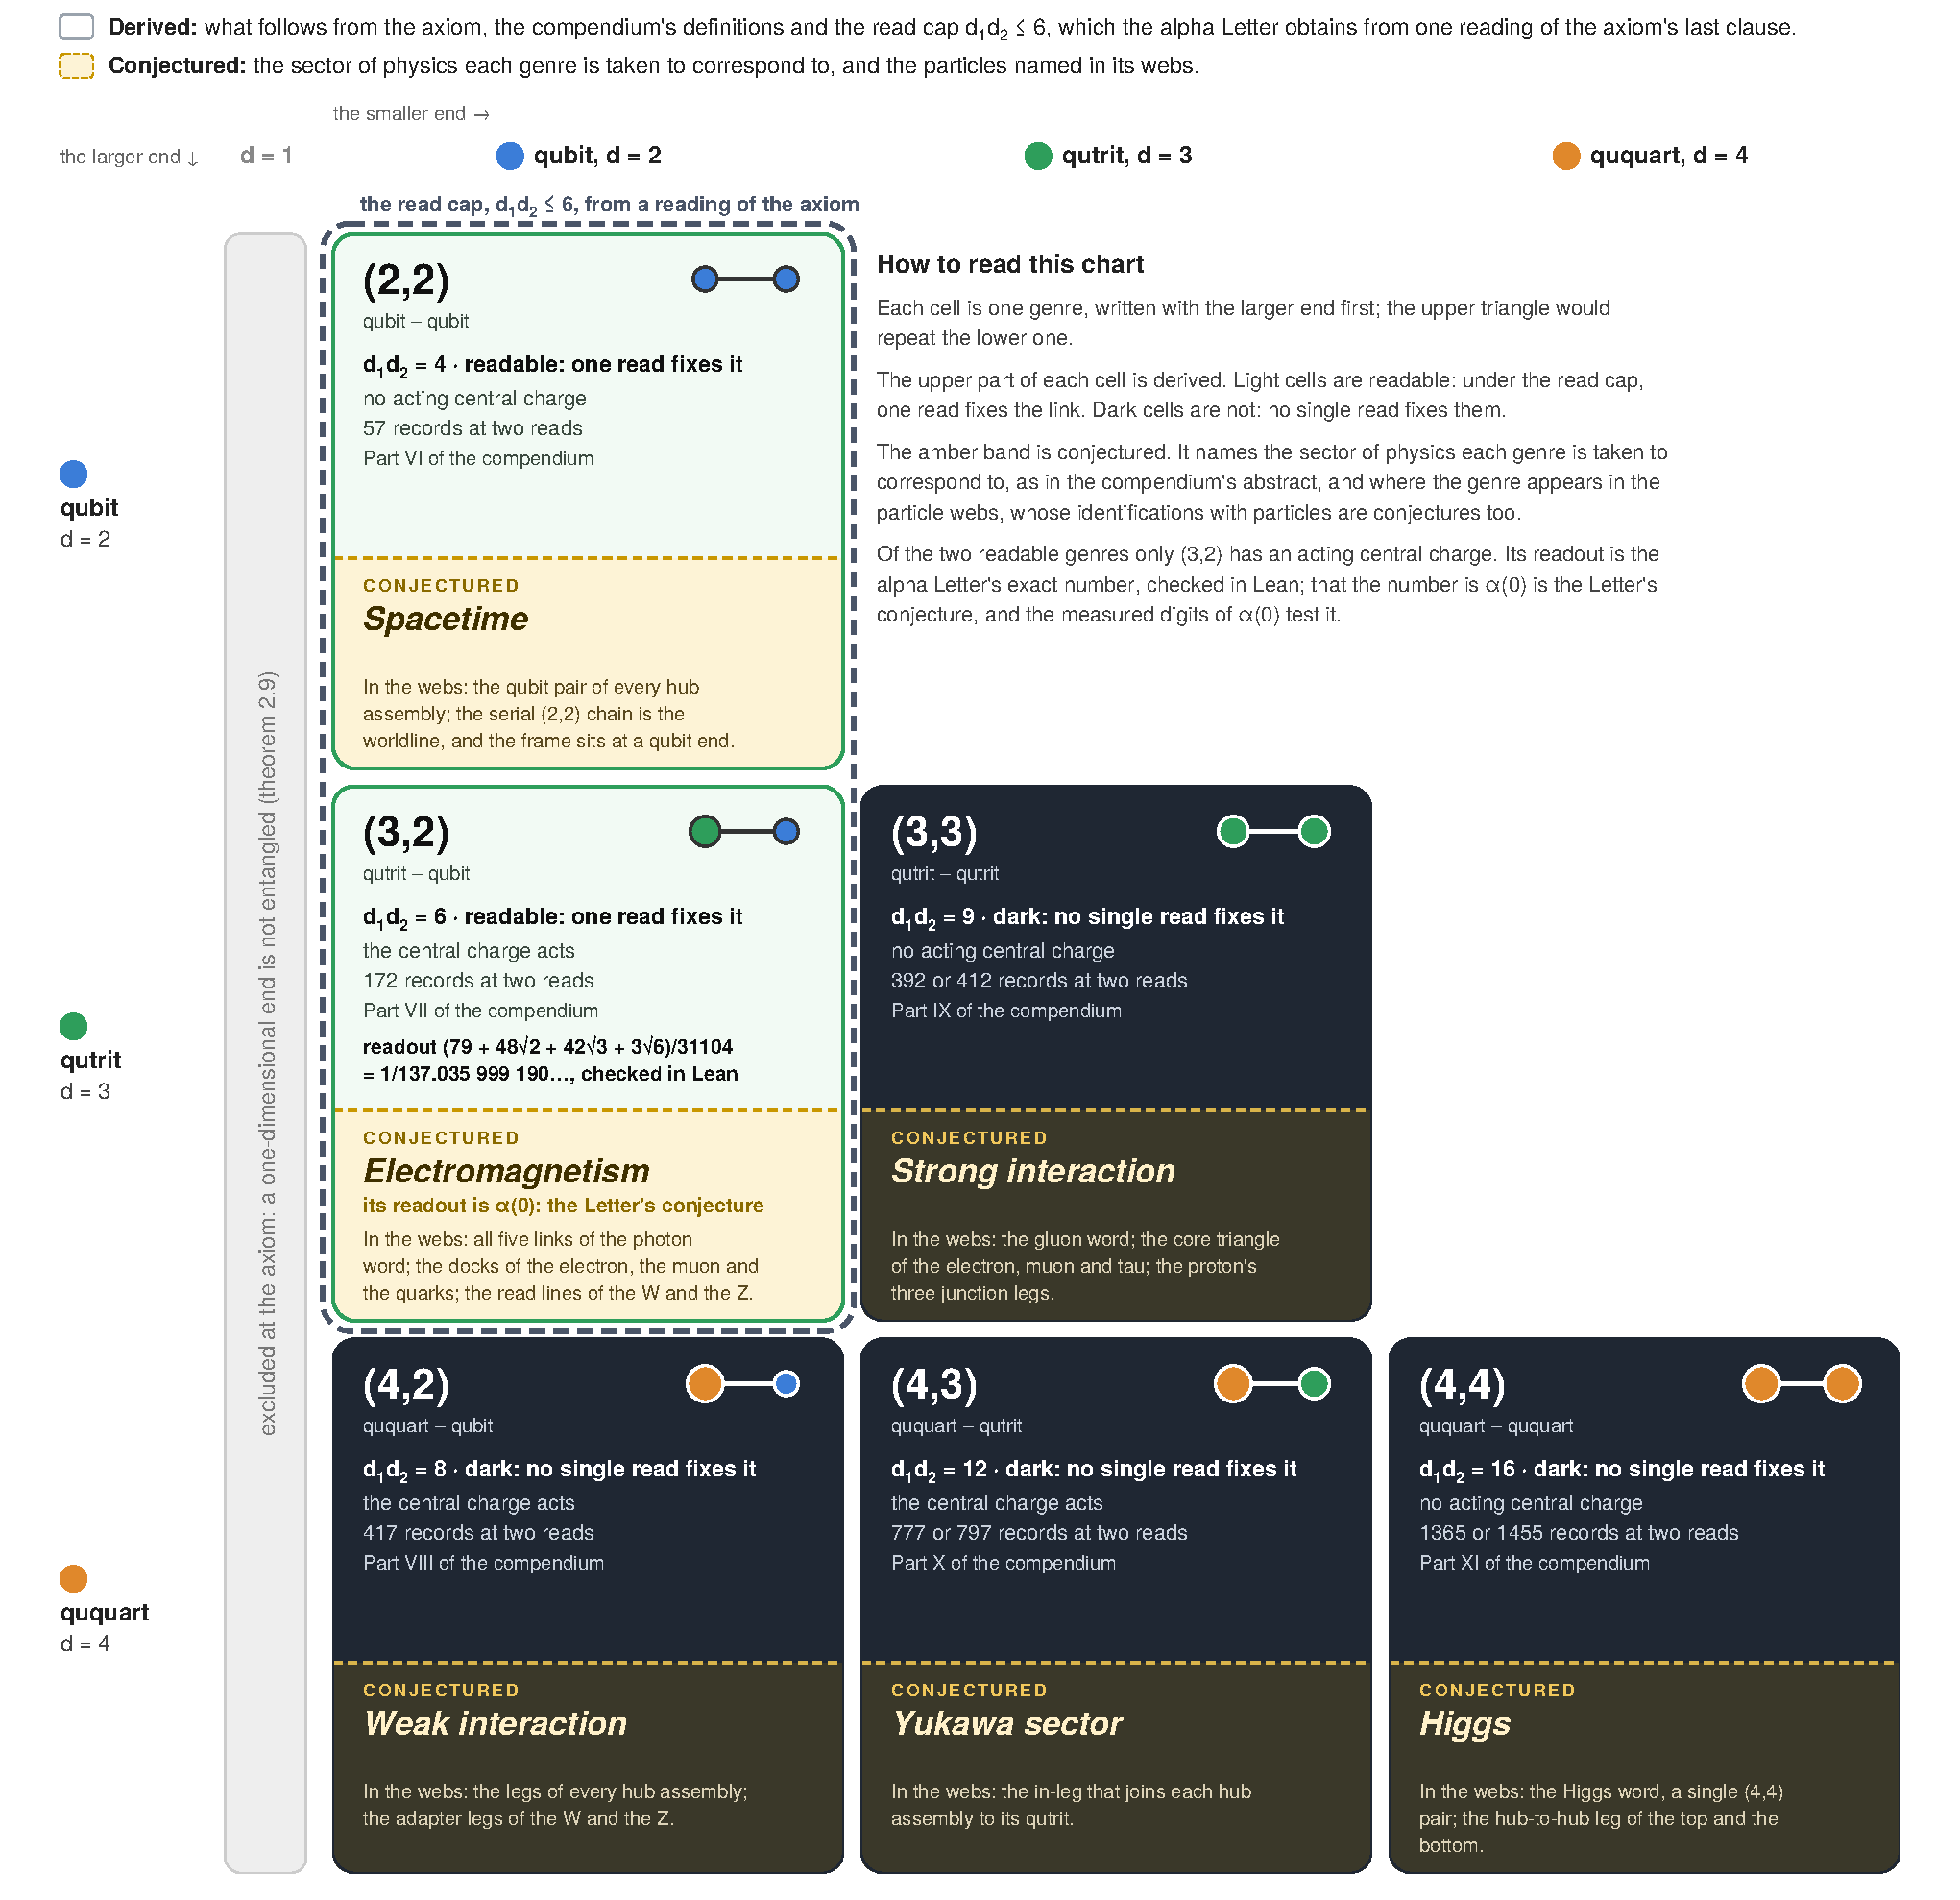
\includegraphics[width=\linewidth]{../figures/genre-matrix.pdf}
\caption{The six genres of the link, with the larger end first. The upper part of each cell is derived; the genres inside the dashed outline are readable, since one read fixes the link when $d_1 d_2 \le 6$, and the others are dark. The band at the foot of each cell is conjectured. The records are those of a link read twice; at (3,3), (4,3) and (4,4) the compendium gives two spellings of the closure sector, and both counts are shown.}\label{fig:genre-matrix}
\end{figure}

The rest of this chapter draws the web the compendium records for each Standard Model particle. That a web is the particle it is named for is a conjecture in every case. What the compendium derives is about the web, and each caption gives the standing of those results and the weakest grade among them. Every site is a qudit and every line a maximally entangled pair; the colour of a site gives its dimension (two blue, three green, four orange), a heavy ring marks a core site and a dashed ring a read site. Laid out as the Standard Model chart in Figure~\ref{fig:particle-chart}, the webs add one hub assembly at each generation. The electron is the core triangle of three qutrits with one hub assembly at a corner, and the muon and the tau carry two and three. The up quark is a qutrit with its docks, and the charm and the top add one and two hubs; the down, the strange and the bottom carry one, two and three; and the three neutrino depth webs carry one, two and three.

The W and the Z are one web, and what distinguishes them is the read: the W is read along one line and the Z along two, drawn heavy. The neutron is not drawn: its recorded body has a hub at degree five and a qutrit at degree four, beyond the valence law (at most $d$ pairs at a qudit of dimension $d$). Each identification of a web with a particle is graded where its result stands, and each figure names that standing. The layouts are for legibility and carry no content.
\begin{figure}[p]\centering
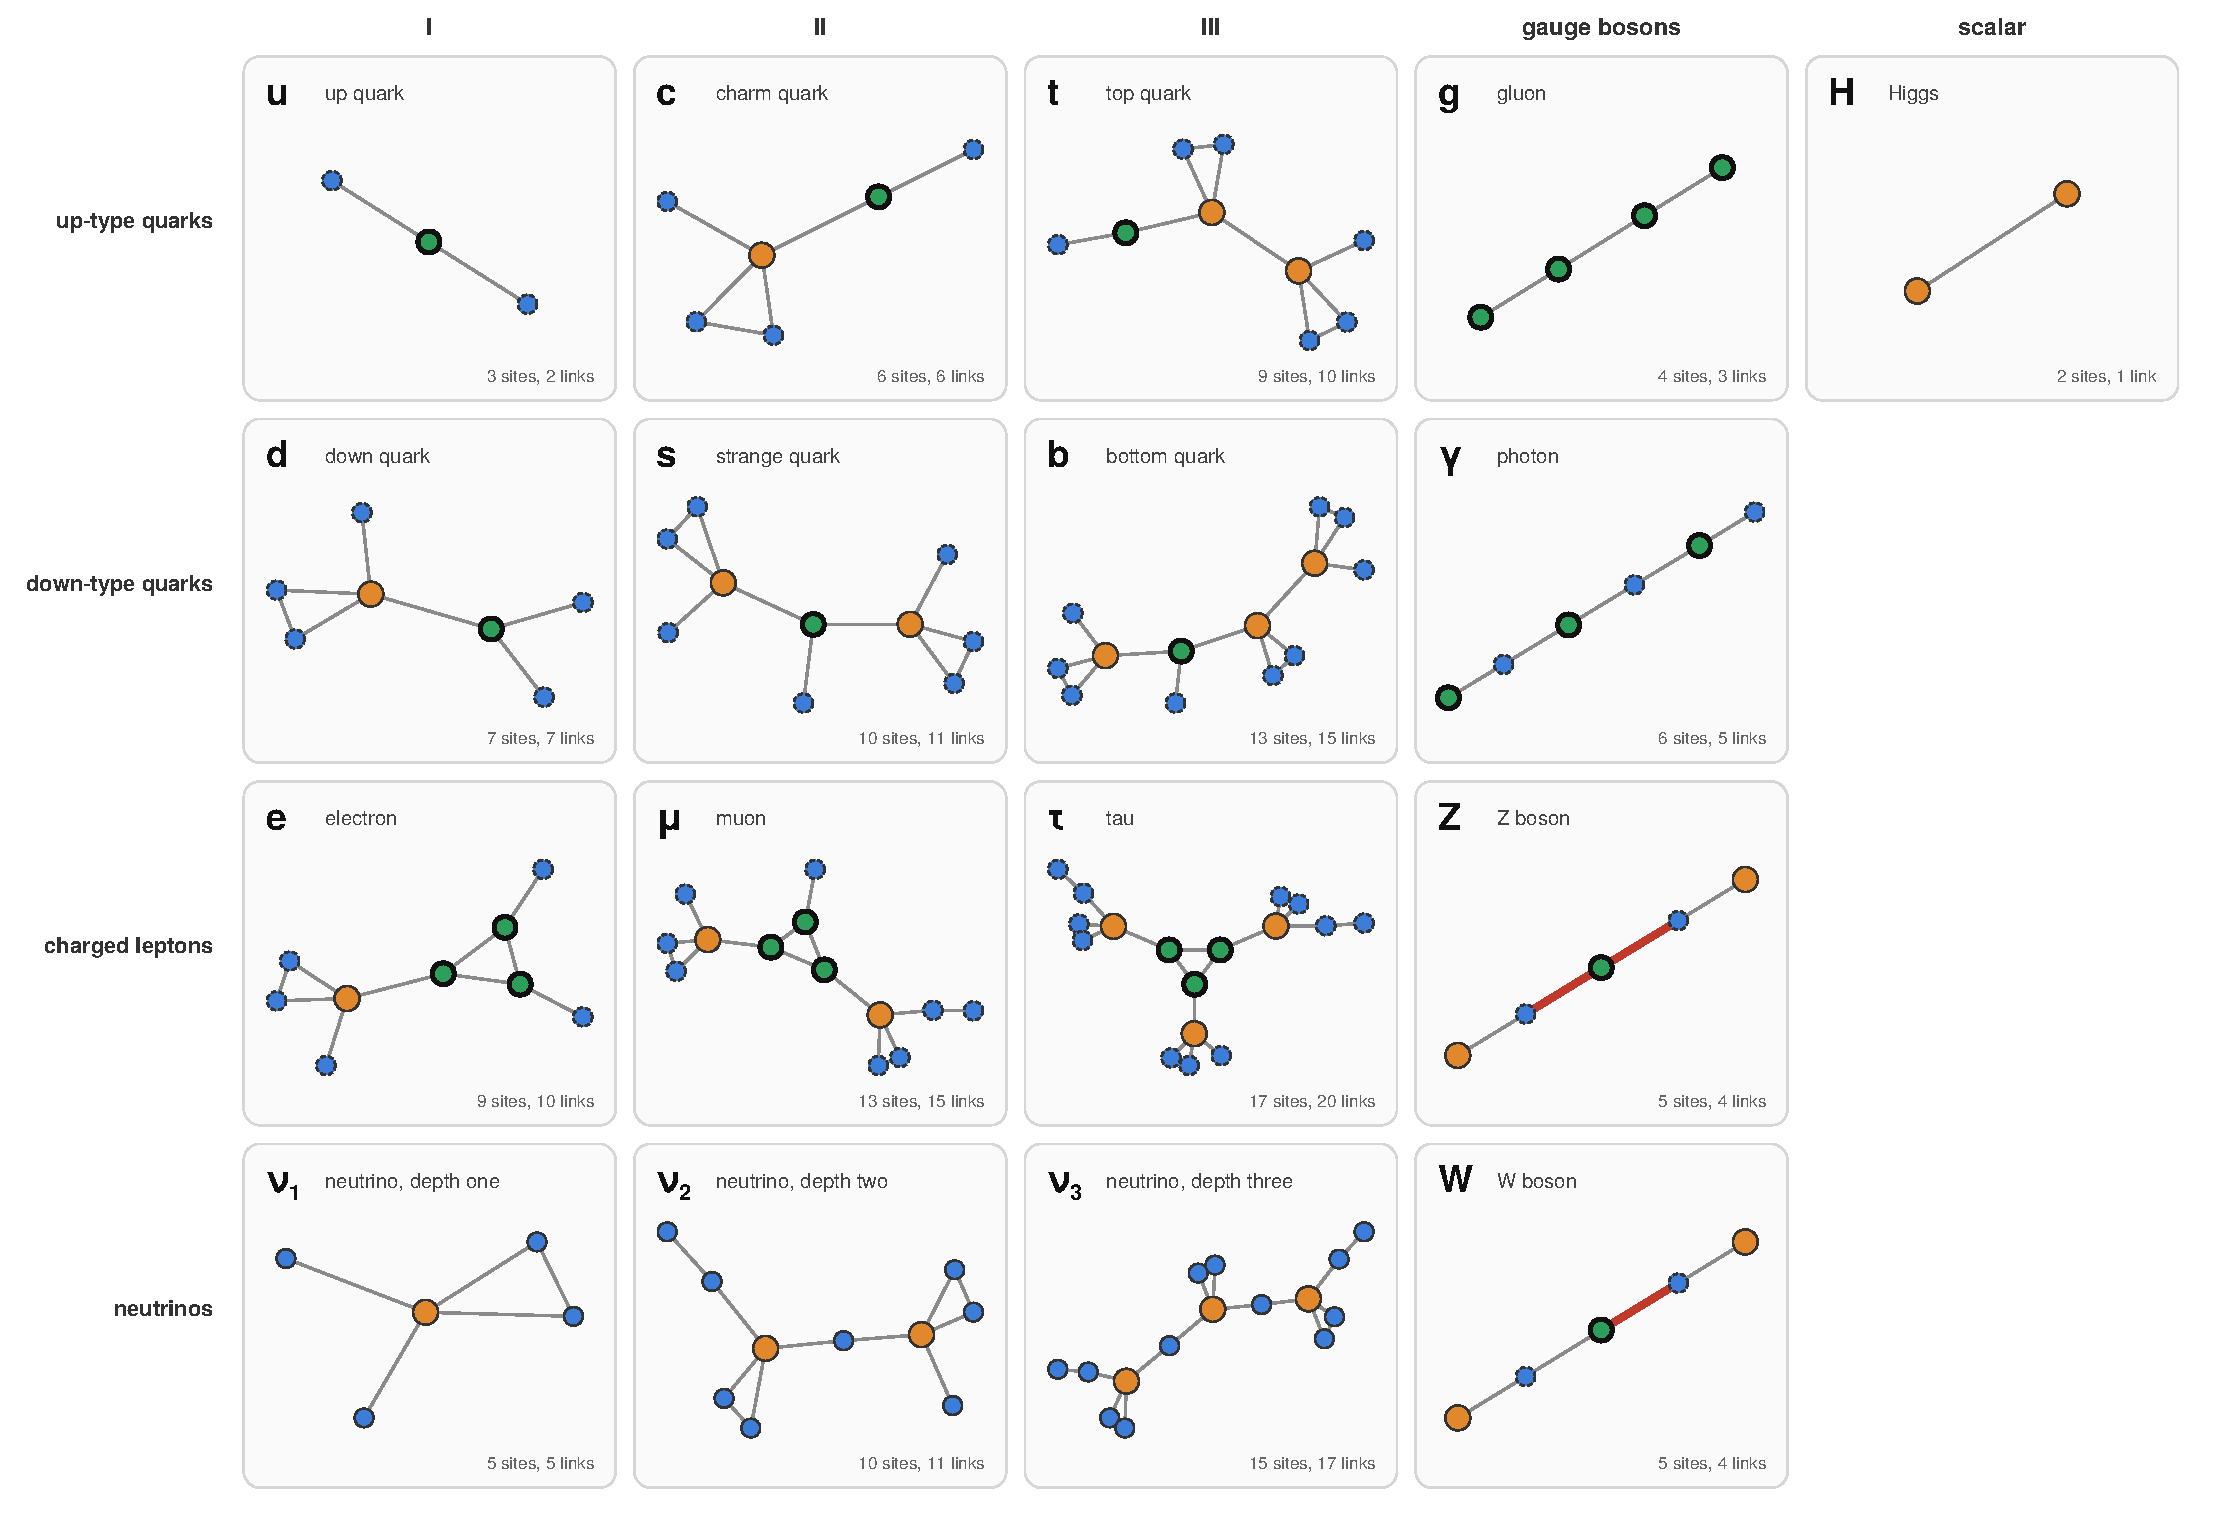
\includegraphics[width=\linewidth]{../figures/standard-model-webs.pdf}
\caption{Conjectured webs for the Standard Model particles, laid out by generation. Each generation adds one hub assembly; the W and the Z are one web, read along one line and along two.}\label{fig:particle-chart}
\end{figure}
\clearpage
\begin{figure}[htbp]\centering
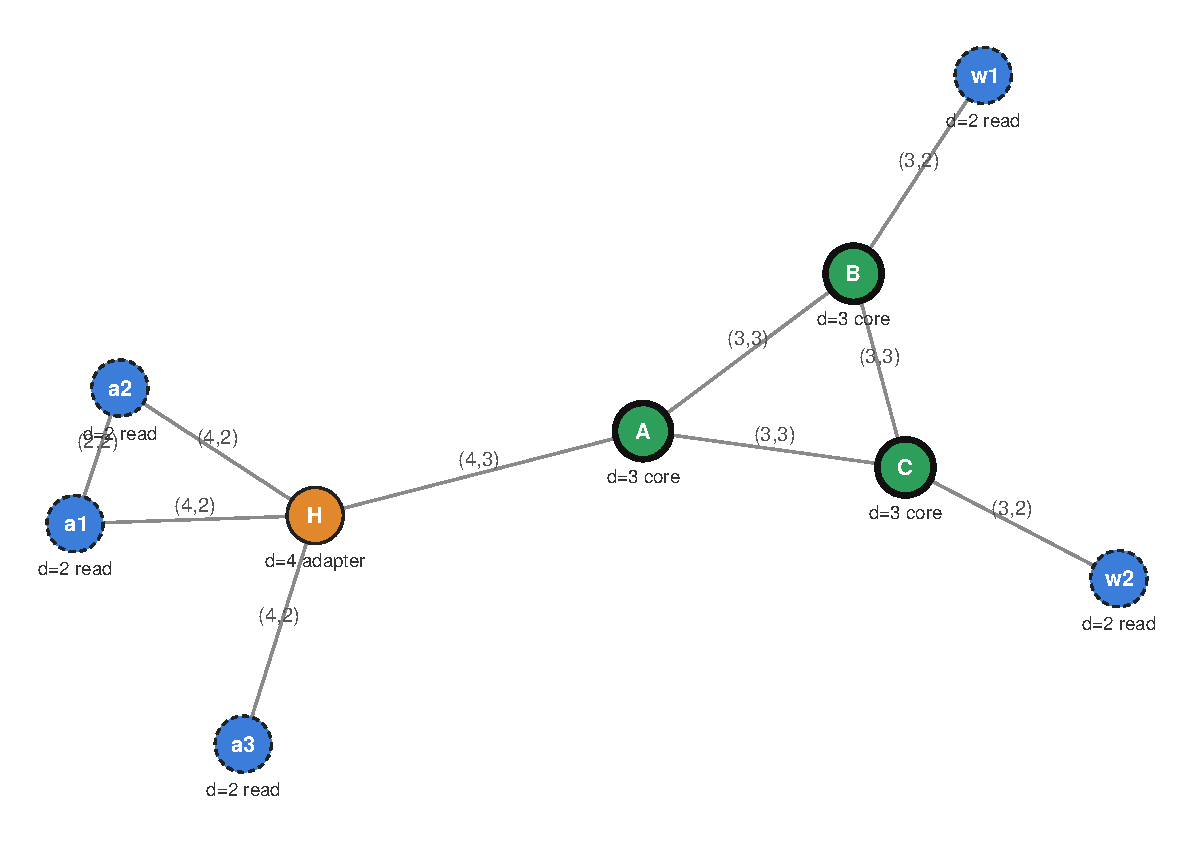
\includegraphics[width=\linewidth,height=0.36\textheight,keepaspectratio]{../figures/webs/electron.pdf}
\caption{\textbf{Electron} (e). The web \texttt{E\_TWODOCK}: 9 sites and 10 links, at the genres (2,2) 1, (3,2) 2, (3,3) 3, (4,2) 3, (4,3) 1. The lepton ladder as hub assemblies, conditional theorem 152.1: the core triangle with one hub assembly. Weakest grade: conditional theorem.}
\label{fig:particle-electron}
\end{figure}
\begin{figure}[htbp]\centering
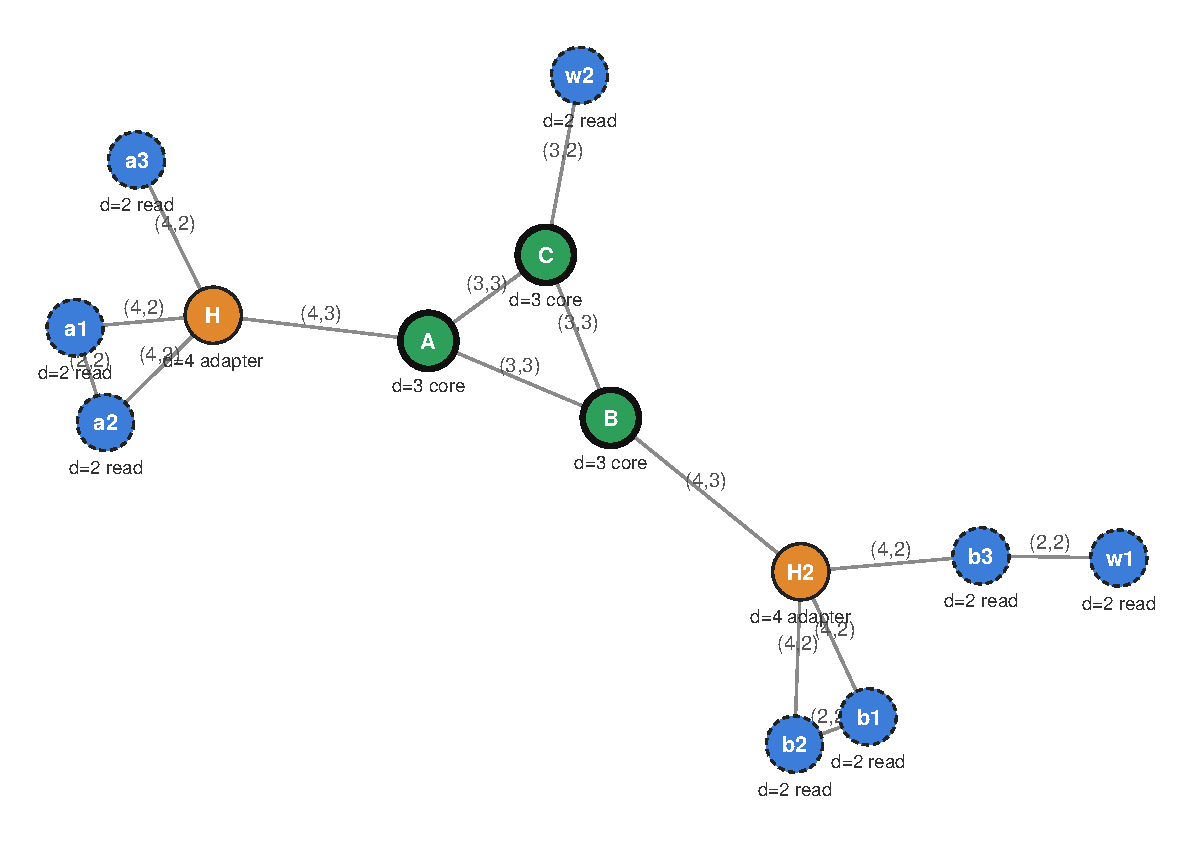
\includegraphics[width=\linewidth,height=0.36\textheight,keepaspectratio]{../figures/webs/muon.pdf}
\caption{\textbf{Muon} ($\mu$). The web \texttt{T6-MU-LEAF}: 13 sites and 15 links, at the genres (2,2) 3, (3,2) 1, (3,3) 3, (4,2) 6, (4,3) 2. The lepton ladder as hub assemblies, conditional theorem 152.1: the core triangle with two hub assemblies. Weakest grade: conditional theorem.}
\label{fig:particle-muon}
\end{figure}
\begin{figure}[htbp]\centering
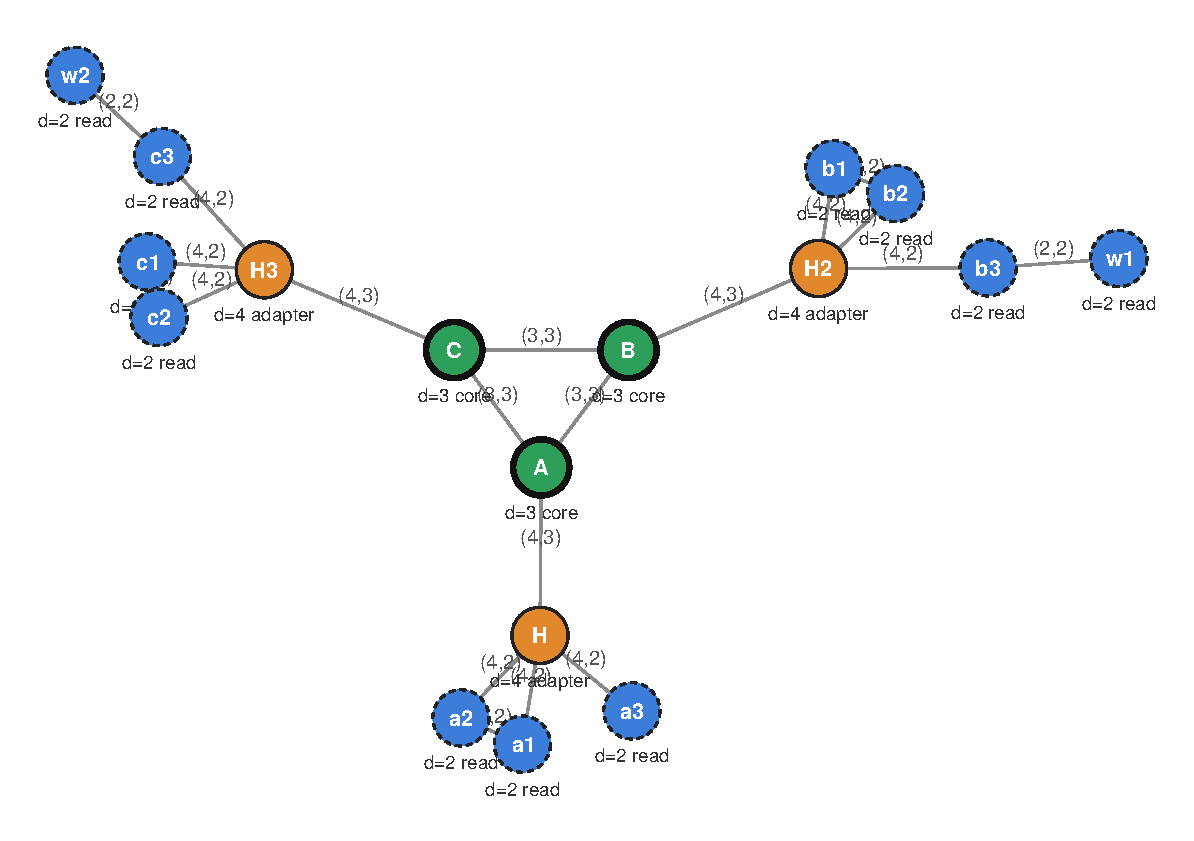
\includegraphics[width=\linewidth,height=0.36\textheight,keepaspectratio]{../figures/webs/tau.pdf}
\caption{\textbf{Tau} ($\tau$). The web \texttt{T6-TAU-LL}: 17 sites and 20 links, at the genres (2,2) 5, (3,3) 3, (4,2) 9, (4,3) 3. The tau as the third hub on the triangle core, theorem 154.1. Weakest grade: theorem.}
\label{fig:particle-tau}
\end{figure}
\begin{figure}[htbp]\centering
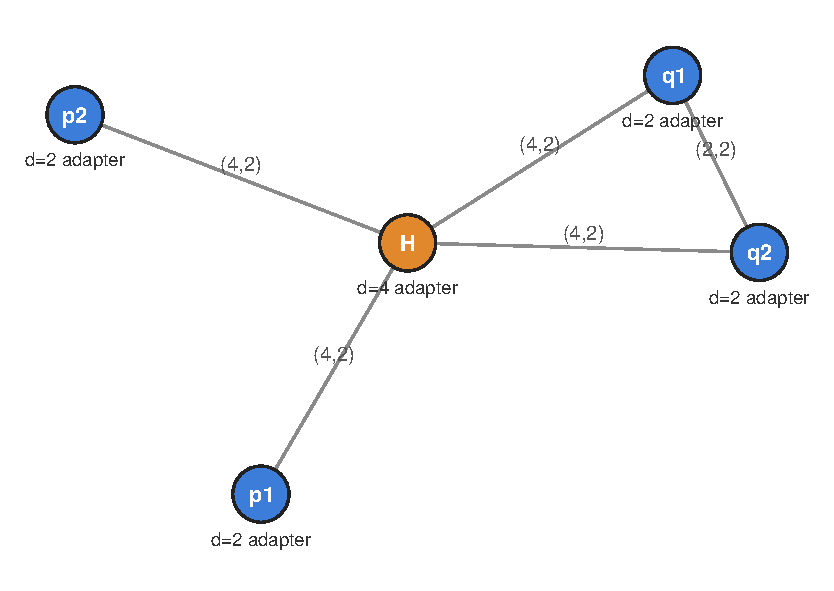
\includegraphics[width=\linewidth,height=0.36\textheight,keepaspectratio]{../figures/webs/neutrino-depth-web-n0-the-cross-core-body.pdf}
\caption{\textbf{The neutrino at depth one} ($\nu_1$). The web \texttt{CROSS-CORE-N0}: 5 sites and 5 links, at the genres (2,2) 1, (4,2) 4. The cross-core body at depth one. Its reading as a neutrino is open; the neutral sinks census is conditional theorem 162.2, and the other candidate webs are open. Weakest grade: open result.}
\label{fig:particle-neutrino-depth-web-n0-the-cross-core-body}
\end{figure}
\begin{figure}[htbp]\centering
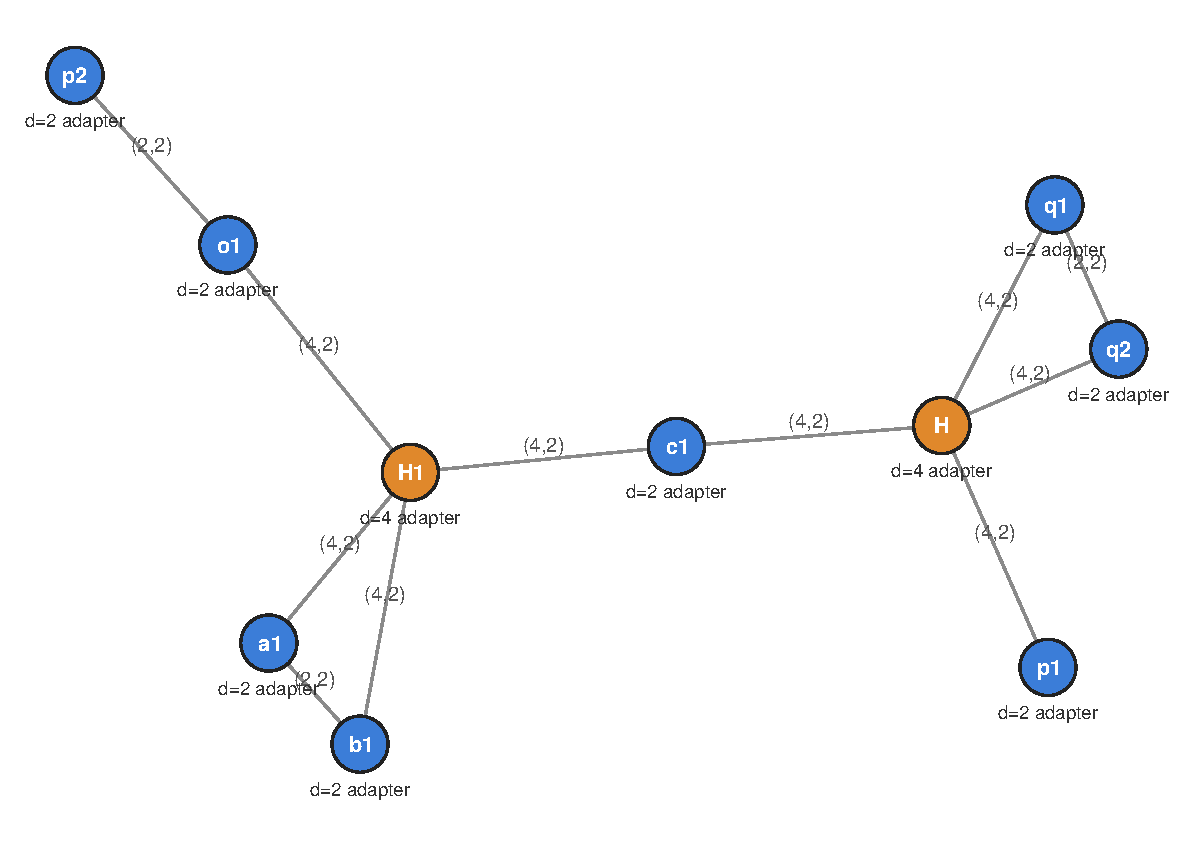
\includegraphics[width=\linewidth,height=0.36\textheight,keepaspectratio]{../figures/webs/neutrino-depth-web-n1-the-cross-core-body.pdf}
\caption{\textbf{The neutrino at depth two} ($\nu_2$). The web \texttt{CROSS-CORE-N1}: 10 sites and 11 links, at the genres (2,2) 3, (4,2) 8. The cross-core body at depth two; standing as for the first. Weakest grade: open result.}
\label{fig:particle-neutrino-depth-web-n1-the-cross-core-body}
\end{figure}
\begin{figure}[htbp]\centering
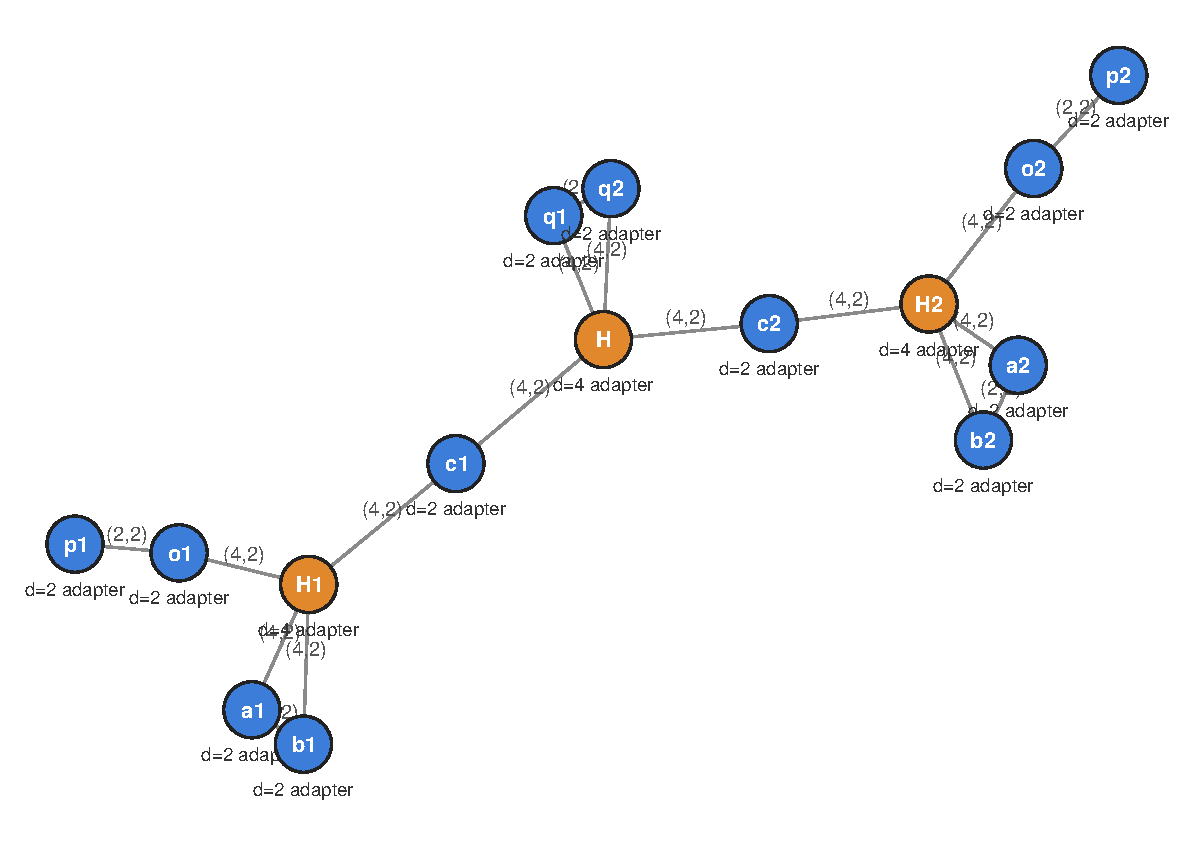
\includegraphics[width=\linewidth,height=0.36\textheight,keepaspectratio]{../figures/webs/neutrino-depth-web-n2-the-cross-core-body.pdf}
\caption{\textbf{The neutrino at depth three} ($\nu_3$). The web \texttt{CROSS-CORE-N2}: 15 sites and 17 links, at the genres (2,2) 5, (4,2) 12. The cross-core body at depth three; standing as for the first. Weakest grade: open result.}
\label{fig:particle-neutrino-depth-web-n2-the-cross-core-body}
\end{figure}
\begin{figure}[htbp]\centering
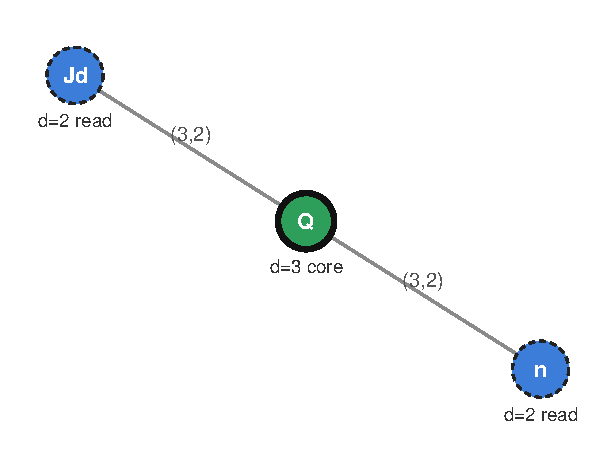
\includegraphics[width=\linewidth,height=0.36\textheight,keepaspectratio]{../figures/webs/up-quark.pdf}
\caption{\textbf{Up quark} (u). The web \texttt{U\_DOCKED}: 3 sites and 2 links, at the genres (3,2) 2. Flavor as the rung name and the quark ladder, conditional theorem 181.2. Weakest grade: conditional theorem.}
\label{fig:particle-up-quark}
\end{figure}
\begin{figure}[htbp]\centering
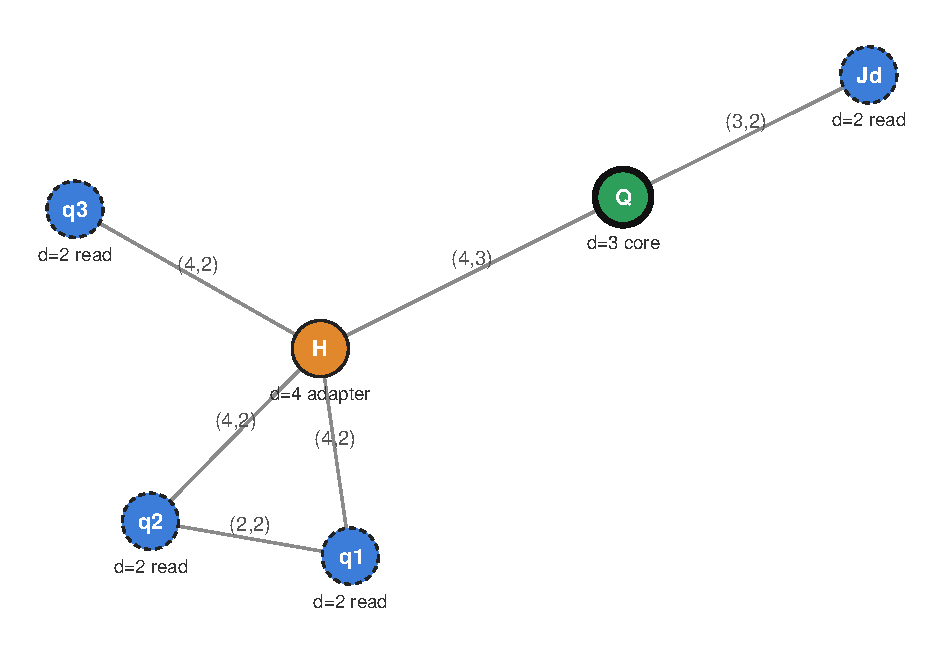
\includegraphics[width=\linewidth,height=0.36\textheight,keepaspectratio]{../figures/webs/charm-quark.pdf}
\caption{\textbf{Charm quark} (c). The web \texttt{C\_DOCKED}: 6 sites and 6 links, at the genres (2,2) 1, (3,2) 1, (4,2) 3, (4,3) 1. The quark ladder, conditional theorems 181.2 and 181.4. Weakest grade: conditional theorem.}
\label{fig:particle-charm-quark}
\end{figure}
\begin{figure}[htbp]\centering
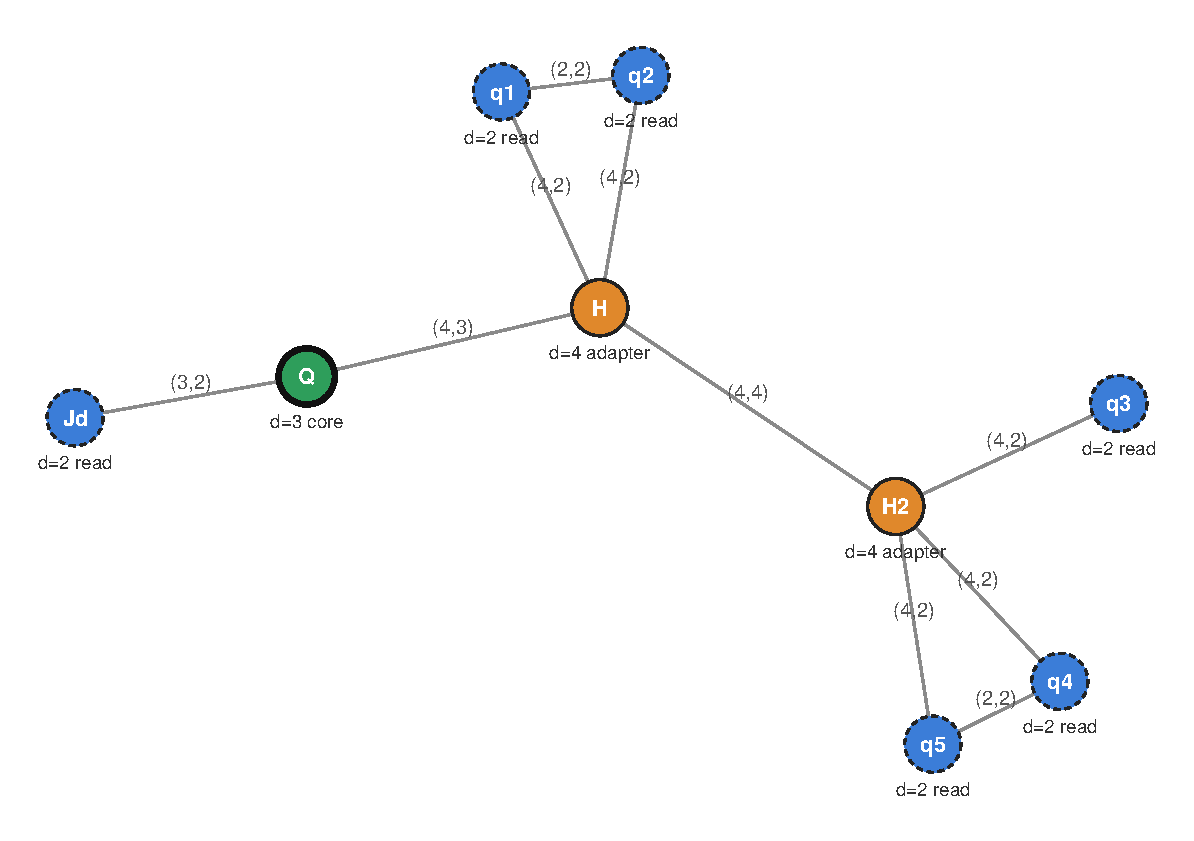
\includegraphics[width=\linewidth,height=0.36\textheight,keepaspectratio]{../figures/webs/top-quark.pdf}
\caption{\textbf{Top quark} (t). The web \texttt{TA\_DOCKED}: 9 sites and 10 links, at the genres (2,2) 2, (3,2) 1, (4,2) 5, (4,3) 1, (4,4) 1. The quark ladder, conditional theorems 181.2 and 181.4. Weakest grade: conditional theorem.}
\label{fig:particle-top-quark}
\end{figure}
\begin{figure}[htbp]\centering
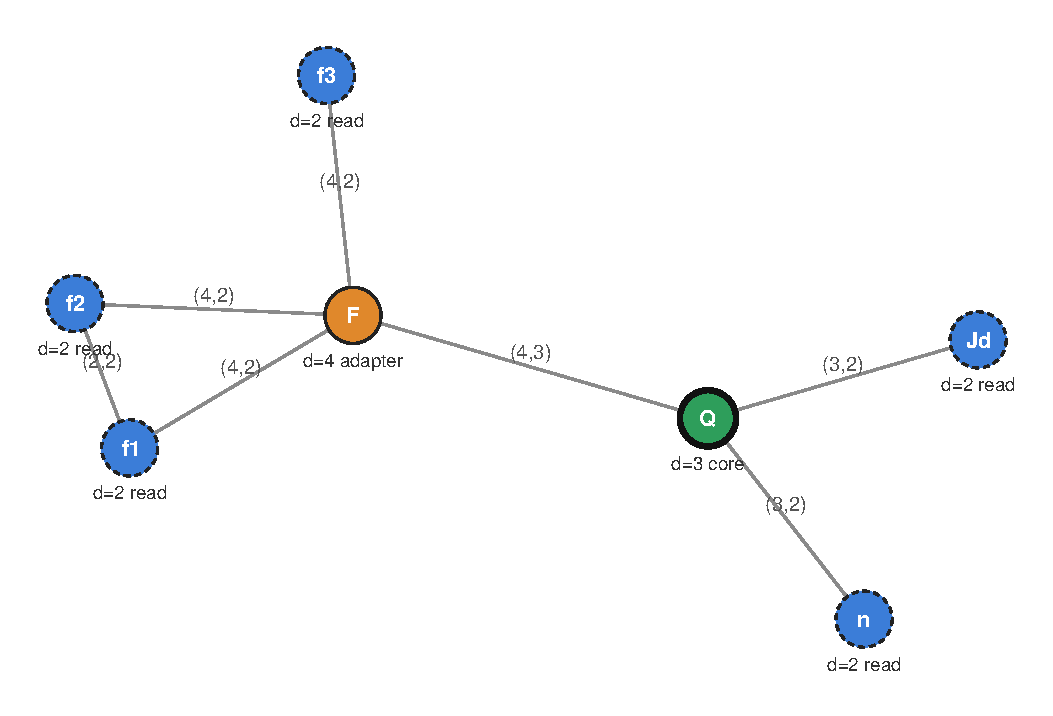
\includegraphics[width=\linewidth,height=0.36\textheight,keepaspectratio]{../figures/webs/down-quark.pdf}
\caption{\textbf{Down quark} (d). The web \texttt{D\_DOCKED}: 7 sites and 7 links, at the genres (2,2) 1, (3,2) 2, (4,2) 3, (4,3) 1. The quark ladder, conditional theorems 181.2 and 181.4. Weakest grade: conditional theorem.}
\label{fig:particle-down-quark}
\end{figure}
\begin{figure}[htbp]\centering
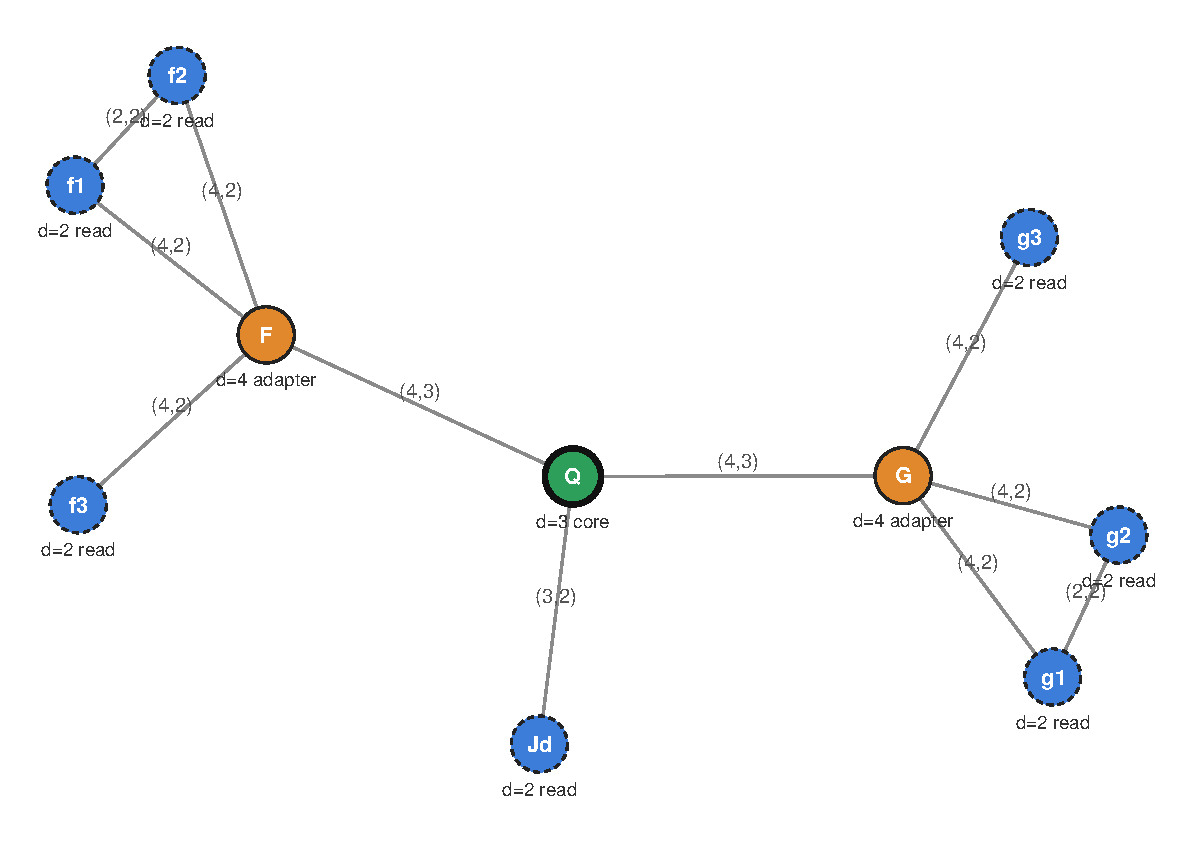
\includegraphics[width=\linewidth,height=0.36\textheight,keepaspectratio]{../figures/webs/strange-quark.pdf}
\caption{\textbf{Strange quark} (s). The web \texttt{S\_DOCKED}: 10 sites and 11 links, at the genres (2,2) 2, (3,2) 1, (4,2) 6, (4,3) 2. The quark ladder, conditional theorems 181.2 and 181.4. Weakest grade: conditional theorem.}
\label{fig:particle-strange-quark}
\end{figure}
\begin{figure}[htbp]\centering
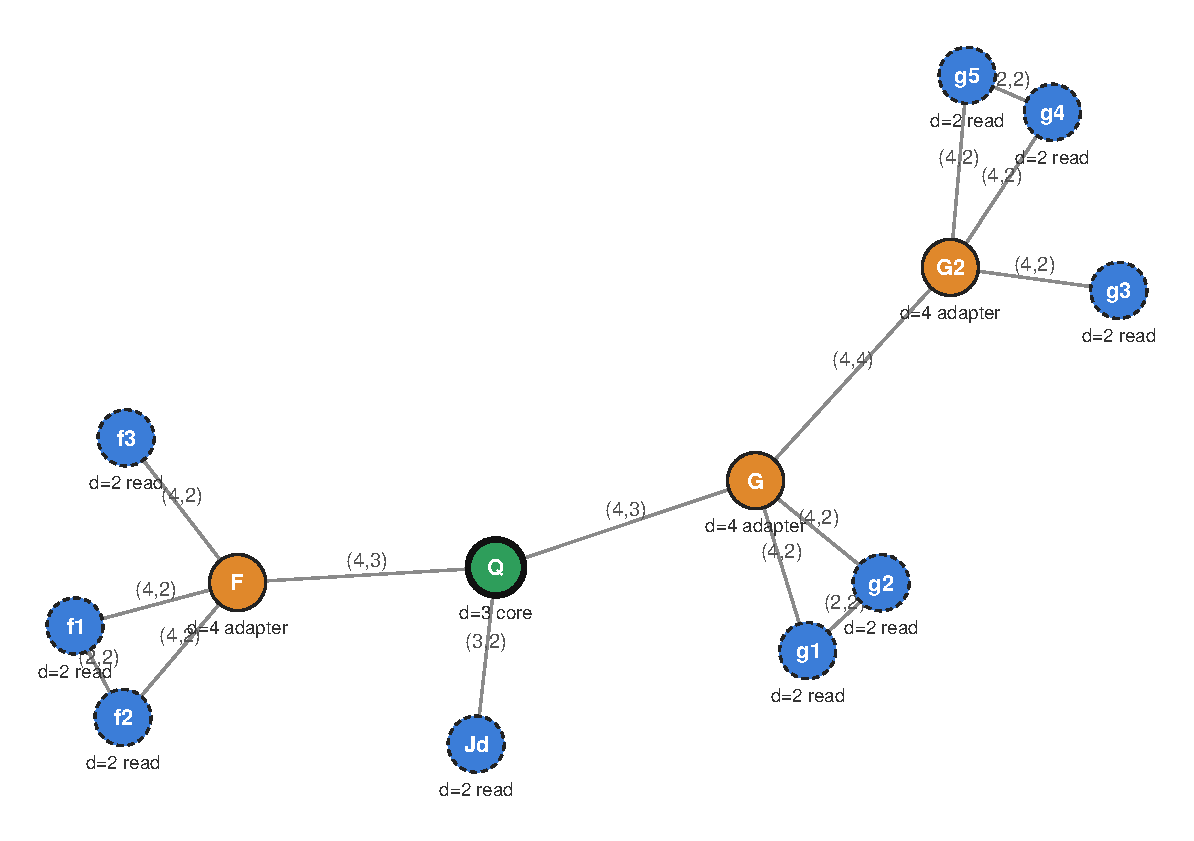
\includegraphics[width=\linewidth,height=0.36\textheight,keepaspectratio]{../figures/webs/bottom-quark.pdf}
\caption{\textbf{Bottom quark} (b). The web \texttt{BA\_DOCKED}: 13 sites and 15 links, at the genres (2,2) 3, (3,2) 1, (4,2) 8, (4,3) 2, (4,4) 1. The quark ladder, conditional theorems 181.2 and 181.4. Weakest grade: conditional theorem.}
\label{fig:particle-bottom-quark}
\end{figure}
\begin{figure}[htbp]\centering
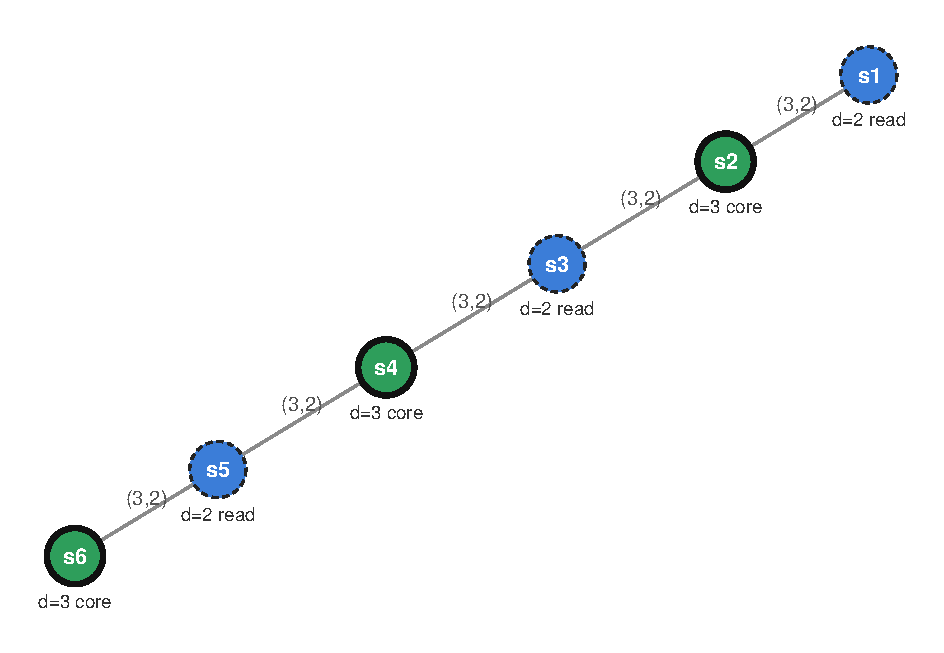
\includegraphics[width=\linewidth,height=0.36\textheight,keepaspectratio]{../figures/webs/photon.pdf}
\caption{\textbf{Photon} ($\gamma$). The web \texttt{r-GAM}: 6 sites and 5 links, at the genres (3,2) 5. The photon word. The (2,3) open link as the photon is theorem 134.1; the photon docks at both faces, conditional theorem 150.1. Weakest grade: conditional theorem.}
\label{fig:particle-photon}
\end{figure}
\begin{figure}[htbp]\centering
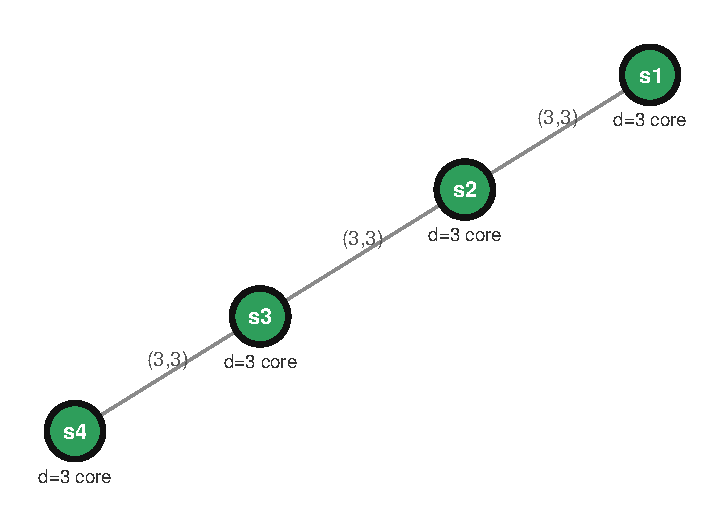
\includegraphics[width=\linewidth,height=0.36\textheight,keepaspectratio]{../figures/webs/gluon.pdf}
\caption{\textbf{Gluon} (g). The web \texttt{r-GLU}: 4 sites and 3 links, at the genres (3,3) 3. The gluon word. The strong coupling as the gluon pair-ket office is conditional theorem 149.1. Weakest grade: conditional theorem.}
\label{fig:particle-gluon}
\end{figure}
\begin{figure}[htbp]\centering
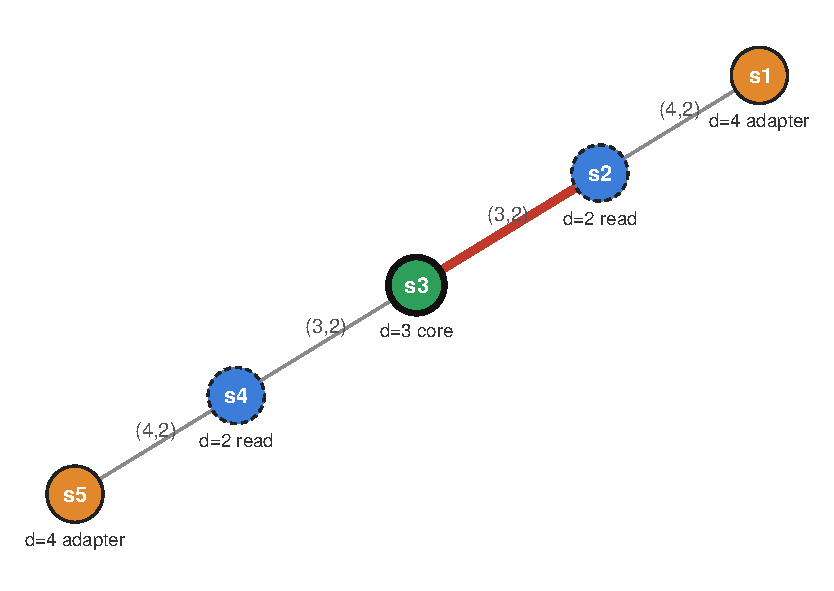
\includegraphics[width=\linewidth,height=0.36\textheight,keepaspectratio]{../figures/webs/w-boson.pdf}
\caption{\textbf{W boson} (W). The web \texttt{r-WPM}: 5 sites and 4 links, at the genres (3,2) 2, (4,2) 2. The W word, read along one line (heavy). The W word as the passage web of the cross read is open result 159.2. Weakest grade: open result.}
\label{fig:particle-w-boson}
\end{figure}
\begin{figure}[htbp]\centering
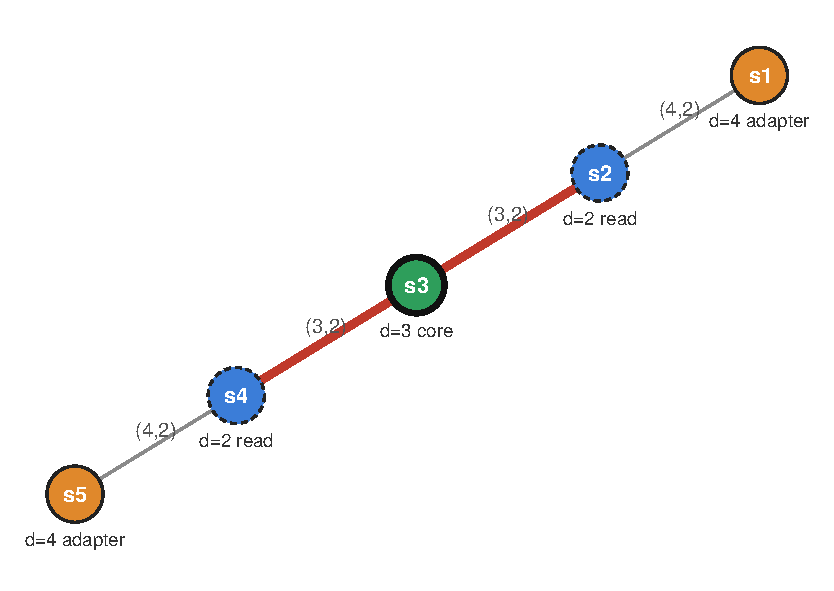
\includegraphics[width=\linewidth,height=0.36\textheight,keepaspectratio]{../figures/webs/z-boson.pdf}
\caption{\textbf{Z boson} (Z). The web \texttt{r-Z0D}: 5 sites and 4 links, at the genres (3,2) 2, (4,2) 2. The same web as the W, read along two lines (heavy): open result 159.1. The ratio of the two offices is 1/2, conditional theorem 164.5; the W over Z mass ratio is open result 160.1. Weakest grade: open result.}
\label{fig:particle-z-boson}
\end{figure}
\begin{figure}[htbp]\centering
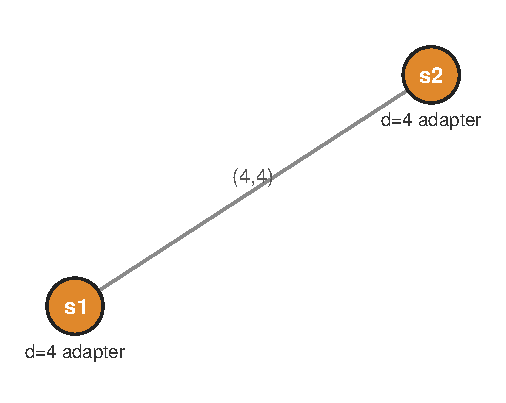
\includegraphics[width=\linewidth,height=0.36\textheight,keepaspectratio]{../figures/webs/higgs.pdf}
\caption{\textbf{Higgs} (H). The web \texttt{r-HIG}: 2 sites and 1 link, at the genres (4,4) 1. The Higgs as the closed hub read, conditional theorem 200.1. Weakest grade: conditional theorem.}
\label{fig:particle-higgs}
\end{figure}
\begin{figure}[htbp]\centering
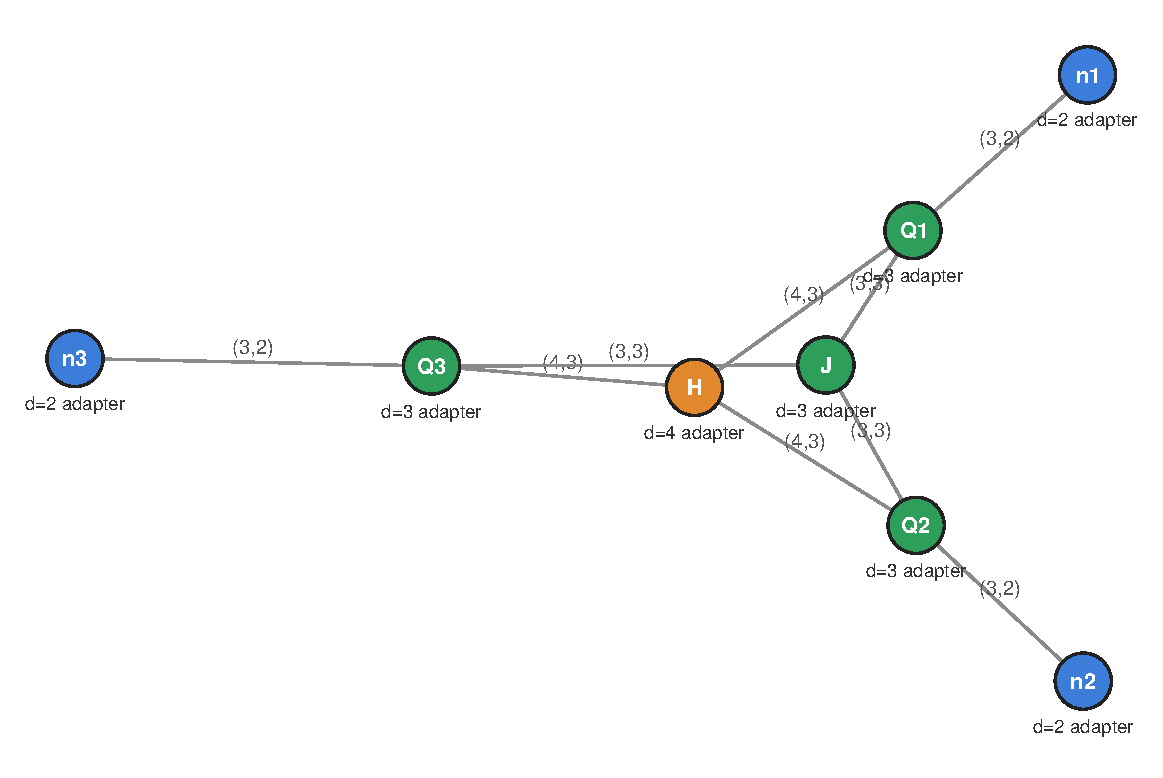
\includegraphics[width=\linewidth,height=0.36\textheight,keepaspectratio]{../figures/webs/proton-the-star-core-of-record.pdf}
\caption{\textbf{The proton} (p). The web \texttt{PROTON-SINK-NAMED}: 8 sites and 9 links, at the genres (3,2) 3, (3,3) 3, (4,3) 3. The proton as a seeded sink: the seeded saturation is open result 175.1 and the joined read at the roster stars conditional theorem 175.2. Its quark content, two ups and a down, is a reading of its three docks and is not derived. Weakest grade: open result.}
\label{fig:particle-proton-the-star-core-of-record}
\end{figure}
\begin{figure}[htbp]\centering
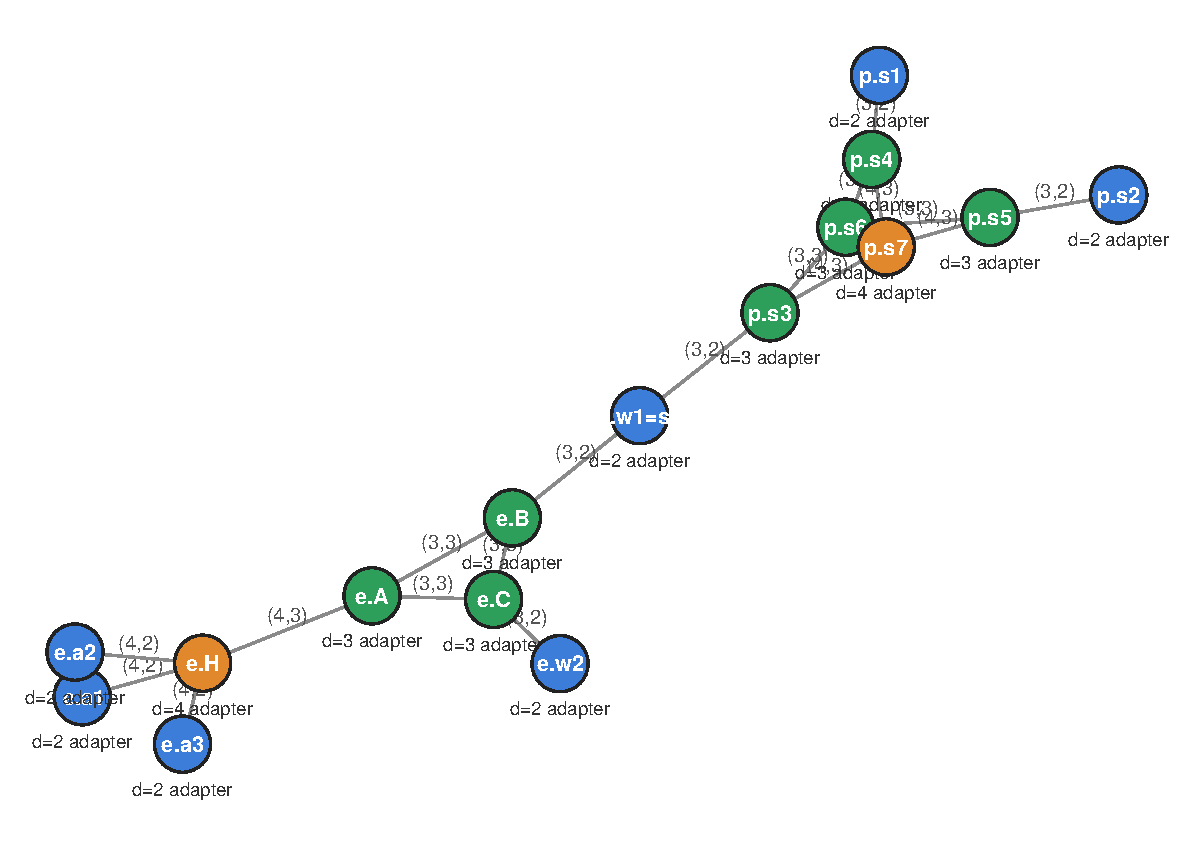
\includegraphics[width=\linewidth,height=0.36\textheight,keepaspectratio]{../figures/webs/hydrogen-the-joined-seed-ep2s1.pdf}
\caption{\textbf{Hydrogen} (H). The web \texttt{SEED-EP2S1}: 16 sites and 19 links, at the genres (2,2) 1, (3,2) 5, (3,3) 6, (4,2) 3, (4,3) 4. The electron web and the proton joined at a shared dock. Hydrogen from the held carrier is conditional theorem 143.1. Weakest grade: conditional theorem.}
\label{fig:particle-hydrogen-the-joined-seed-ep2s1}
\end{figure}
\clearpage
\endgroup
\label{atlaspart:particle-websend}

\clearpage
\label{atlaspart:instruments}
\part*{Instruments}
\addcontentsline{toc}{part}{Instruments}
\setcounter{section}{0}
\renewcommand{\thesection}{I.\arabic{section}}
\section*{The instrument chapters}
\addcontentsline{toc}{section}{The instrument chapters}
Each Part lists its instrument chapters in its chapter titled \emph{The instrument tables of this Part}. They are printed here, in the order those chapters list them, with the comments removed as in the rest of this compendium. They are numbered I.1 to I.52, so that no number in the Parts changes. Each one names the Part that lists it.
\section{The Rosetta table in full}\label{mod:I-7-rosetta-table-in-full}
\chdesig{1-7}{}{I-7-rosetta-table-in-full}{I-7-rosetta-table-in-full}
\chinstrument{I}{faedb00dcabbfb29}
\begin{chtable}[The Rosetta table of the Chain Theory nouns]
This chapter lays the Rosetta table in full: every noun of the theory at one line, the noun, the nearest standard concept, the distance and its clause, one hundred twenty-seven nouns in the order of the adopted table, the distances exact at thirty-six, nearest at eighty-nine and none at two.
\end{chtable}
\chstanding{instrument}
\chdeps{}{}
\begin{chtheorem}
\begin{itemize}
\item \rosetta{link}{a maximally entangled pair of two qudits}: exact; the same object: the pair of the Axiom, its two ends the qudits
\item \rosetta{record}{an invariant jointly fixed by a set of projective measurements}: nearest; fixed by all reads of a qudit taken jointly under every matching of basis directions, a Weyl letter at each slot and not one outcome
\item \rosetta{read}{a projective measurement in a basis, passed along the pair}: nearest; an entanglement swap of the qudit with another in one basis, giving the qudit its only basis and carrying it to the far end
\item \rosetta{wash}{the twirl: the average over the unfixed basis identifications}: exact; the same operation: the group average over the identifications the definitions leave free; measurement as the wash at one act
\item \rosetta{move}{an elementary LOCC-like operation on the network of pairs}: nearest; one of the admitted move kinds (mirror, subdivide, duplicate, delete, cut, composite join) acting on the links of a web and not on a state vector
\item \rosetta{web}{a graph state: a tensor network of maximally entangled pairs}: nearest; the ends are qudits shared between pairs, with no stabiliser phase fixed and no measurement pattern chosen
\item \rosetta{hub}{a junction vertex of degree three or more}: nearest; a pair read as a qudit, the (2,2) pair whose legs open the qutrits of a body
\item \rosetta{dock}{a leaf pair at a terminal qubit, a dangling edge}: nearest; a (2,2) link whose far end is washed, the charge register of a body
\item \rosetta{core}{the root vertex of a tree-shaped state}: nearest; the site the closure closes at, the one link of a body opened
\item \rosetta{sink}{a fixed point of the dynamics, a stable particle}: nearest; a web no admitted move leaves, its forward edge empty; named the particle by correspondence
\item \rosetta{seed}{the initial state of an iterated map}: nearest; a listed web run as its own seed at wave zero under the stop reading
\item \rosetta{wave}{one layer of a breadth-first closure}: nearest; the webs first reached at one count of moves from the seed
\item \rosetta{saturation}{the iteration of a map to its fixed point}: nearest; the forward closure of a seed terminating at the stop condition, the sinks printed
\item \rosetta{closure}{the forward closure of a set under operations}: exact; the same object: the orbit of the seed under the admitted moves, graded by waves
\item \rosetta{genre}{the pair of local dimensions of an entangled pair}: exact; the same object: the pair type (a,b) of the two ends
\item \rosetta{register}{a Hilbert-space dimension, the dimension of an operator space}: nearest; a product of site dimensions, the space a read or a body is traced over
\item \rosetta{office}{the first-order coefficient of a matrix element}: nearest; the first-order read at the common support of a body, the register of the read at one link
\item \rosetta{strike}{no standard concept}: none; A strike removes from a readout the record of one pair the qudit meets, the far end of that pair left unread.
\item \rosetta{the act}{a Bell-basis projection of two qudits, an entanglement swap}: exact; the same operation: distilling, the projection of any two qudits onto a pair on their common support
\item \rosetta{the one link}{a single maximally entangled pair, two qudits}: exact; the same object: one pair of the Axiom read at both ends
\item \rosetta{the Born count}{the normalizing trace of the Born rule}: nearest; the count of records at the full web, the dressed measure a readout is normalized by
\item \rosetta{the gain}{the multiplicity of a projector, a Schmidt rank}: nearest; the product of the dimensions of the ends a read passes, its root the readout
\item \rosetta{the readout}{the expectation value of a projector in the pair state}: nearest; the normalized projector trace at a derived register with the twirl applied
\item \rosetta{the first power}{the first-order term of the coupling expansion}: nearest; the sum of the act readouts of a web, the grading by exchanges at order one
\item \rosetta{the carrier}{a gauge boson, a force carrier}: nearest; the closed read of a readable genre; named the boson by correspondence, as in the glossary
\item \rosetta{the body}{the state of a particle}: nearest; the web of a particle, a network of pairs and not a state vector
\item \rosetta{the probe}{the apparatus of a measurement}: nearest; the measuring body attached at a port, read with the body it measures
\item \rosetta{the attach site}{an interaction vertex}: nearest; the qudit at which one body is joined to another by a pairing
\item \rosetta{the leg}{an edge incident to a vertex}: nearest; a link at a hub carrying one copy, its far-end dimension the dressing
\item \rosetta{the arm}{a half-edge of a graph at a vertex}: exact; the same object: a link at a site
\item \rosetta{the dart}{a directed edge of a graph}: nearest; the oriented read link that carries a charge sign, the read of one link as a signed unit
\item \emph{the frame family} (an equivalence class of reference frames): nearest; the open set at the read, the chain family modulo junctions
\item \rosetta{the slot}{a tensor factor of the register}: exact; the same object: one site position in the product of site dimensions
\item \rosetta{the holonomy}{the holonomy of a connection around a loop}: exact; the same object: the basis transport around a closed path of the web, a unitary on the register
\item \rosetta{the transport}{parallel transport along an edge}: nearest; the passing of a basis along a pair to its far end, fixed by the pair and chosen by no connection
\item \rosetta{the order parameter W}{an order parameter labelling a phase}: nearest; the family of the sinks reached at the stop condition, a discrete label and no field
\item \rosetta{the stop condition}{a termination criterion of an iteration}: nearest; the stop reading of the closure at the pairing-move sink (K2)
\item \rosetta{the pairing move}{an entanglement swap creating a pair between two ends}: nearest; the move that pairs two open ends into one link, its sink set the roster
\item \rosetta{the hub step}{a decay vertex of a decay graph}: nearest; the move that raises or lowers the degree of a hub, the edge of the decay graph
\item \rosetta{the junction}{a trivalent vertex}: nearest; a qutrit site of degree three, the share of three arms at one qudit
\item \rosetta{the released object}{a decay product}: nearest; the web parted off by a move, the cross per depth
\item \emph{the network list} (a fixed library of graph states, a benchmark set): nearest; the fixed list of sixty-four networks the computations run on, used as material and not as a premise
\item \rosetta{the roster}{the particle spectrum, the list of stable states}: nearest; the family of networks the rules admit, the sink set of the pairing move
\item \rosetta{the ladder}{a tower of excitations}: nearest; the sequence of bodies by hub lowering, the order grading of the sum over records
\item \rosetta{the rung}{an energy level, a generation index}: nearest; one step of the ladder, the depth level of the closure
\item \rosetta{the depth}{the circuit depth, the number of rounds}: nearest; the growth order of the closure, the count of waves to the horizon
\item \rosetta{the horizon web}{a causal horizon, the boundary of a light cone}: nearest; the web reached at the depth of the closure, an interface
\item \rosetta{the tick}{the lattice spacing in the step direction}: nearest; one link per step of the lattice of ticks, the order coordinate
\item \rosetta{the unit}{a unit of measure, a normalization}: nearest; the mass unit at the probe hub leg, the dock-struck electron readout
\item \rosetta{qudit}{a d-dimensional quantum system}: exact; the same object: a finite-dimensional quantum system
\item \rosetta{shared}{a qudit entangled with two or more partners}: nearest; a qudit that is one end of two or more pairs; the standard concept carries no pair structure
\item \rosetta{distilling}{a Bell-basis projection, an entanglement swap}: nearest; the projection of two qudits onto a pair on their common support; the standard distillation, the extraction of pairs by local operations and classical communication, is another object
\item \rosetta{known}{the commutant-fixed invariants of a stabilizer}: nearest; what all reads of a qudit taken jointly fix with certainty whichever way basis directions are matched
\item \rosetta{the pair}{a maximally entangled pair of qudits}: exact; the same object: the pair of the Axiom
\item \rosetta{the far end}{the partner qudit of an entangled pair}: exact; the same object: the other end of a pair the qudit meets
\item \rosetta{the common support}{the intersection of the supports of two projectors}: exact; the same object: the common support of two qudits
\item \rosetta{the pair type}{the pair of local dimensions (a,b)}: exact; the same object: the dimensions of the two ends in one fixed orientation
\item \rosetta{the site}{a vertex of a tensor network}: exact; the same object: a qudit of the network
\item \rosetta{the star}{a star graph, a vertex with its incident edges}: exact; the same object: a site with its arms
\item \rosetta{the fine-structure star}{a graph state on a star of three edges}: nearest; a qutrit of degree three with three (3,2) arms, two read and one held
\item \rosetta{the letter}{a generalized Pauli (Weyl) operator}: exact; the same object: the byproduct operator a distillation leaves at a slot
\item \rosetta{the passage}{a non-backtracking walk on a graph}: exact; the same object: a non-backtracking walk of the network
\item \rosetta{the arrow}{a directed edge}: exact; the same object: a direction on a link
\item \rosetta{the attachment pair}{a coupling edge between two subsystems}: nearest; the pair through which a body is read
\item \rosetta{the port}{an open leg of a tensor}: nearest; the read arm of a body at its attachment
\item \rosetta{the copy}{a ket index or a bra index of a tensor}: exact; the same object: in the copy model every link joins one ket end and one bra end
\item \rosetta{the ket end}{the ket index of a tensor factor}: exact; the same object: the ket end of a link
\item \rosetta{the bra end}{the bra index of a tensor factor}: exact; the same object: the bra end of a link
\item \rosetta{the interface}{a bipartition cut of a network}: exact; the same object: the cut between two regions across which reads are counted
\item \rosetta{the join}{the composition of two tensor networks along shared sites}: nearest; the move that joins two webs at shared qudits, one of the interaction kinds (cut, composite join)
\item \rosetta{the joined web}{the composite system of two bodies}: nearest; the web of two bodies joined at their attach sites, read as one
\item \rosetta{the lattice}{a periodic lattice of qudits}: nearest; the periodic join of listed bodies, one link per tick, the lattice of ticks
\item \rosetta{the word}{a Pauli word, a syndrome string}: nearest; the read word of a carrier at a readable link (the photon word, the W word), a product of letters
\item \emph{the sum over records} (a finite sum over paths, a path integral): nearest; the finite sum over the records of a web graded by the exchange count
\item \rosetta{the washed marginal}{a reduced density matrix with the twirl applied}: exact; the same object: the marginal at the cap with the wash applied
\item \rosetta{the cap}{a cutoff on the depth of an iteration}: nearest; the depth at which a closure is read, the bound of a reading
\item \rosetta{the closed read}{a closed walk of measurements, a loop}: nearest; a read whose basis returns to its start, the carrier at a readable genre
\item \rosetta{the open end}{a dangling edge of a tensor network}: exact; the same object: an end of a link not paired at a read
\item \rosetta{the face}{no standard concept}: none; A face is one of two readings of a word the reads admit, printed beside each other with neither preferred.
\item \rosetta{the frame}{a basis choice at a site}: exact; the same object: the basis a read gives a qudit
\item \rosetta{the corner frame}{an eigenbasis at a corner of a lattice cell}: nearest; the frame at a corner of the depth lattice, its overlaps the mixing
\item \rosetta{the dark genre}{a hidden sector, an unobservable sector}: nearest; a genre whose link admits no read at the one link, (3,3) among them
\item \rosetta{the readable genre}{an observable sector}: nearest; a genre whose one link admits a read, six admitted
\item \rosetta{the boundary count}{the entanglement entropy across a cut}: nearest; the count of reads across an interface, a count and no entropy
\item \rosetta{the register tower}{a tower of Hilbert spaces of growing dimension}: nearest; the registers of the depth ladder, one per rung
\item \rosetta{the acting centre}{the centre of an algebra of observables}: nearest; the shared qudit of a readable link at which the act acts, the one at the (2,3) link
\item \rosetta{the scale}{a renormalization scale}: nearest; a body through which a coupling is read, the scale a body
\item \rosetta{the Born square}{the Born probability, the squared amplitude}: exact; the same object: the square of the read at the Born rule
\item \rosetta{the washed square}{the twirled squared amplitude}: exact; the same object: the square of the read with the wash applied, the rate
\item \rosetta{the identification}{a basis identification between two qudits}: exact; the same object: the matching of basis directions across a pair
\item \rosetta{the cut}{the removal of an edge from a graph}: nearest; the move that cuts a link of a web, the reverse of the pairing
\item \rosetta{the self-term}{a self-energy term}: nearest; the record of a body read through itself at the joined web
\item \rosetta{the cross term}{an interference term}: nearest; the record of two bodies read across their join at the joined web
\item \rosetta{the pair ket}{the maximally entangled state vector of a pair}: exact; the same object: the twirl-fixed point, the unique pure state the matchings leave fixed
\item \rosetta{the doublet}{a two-dimensional representation, a spin doublet}: nearest; the doublet content at the closed read, the qubit end pair of a read
\item \rosetta{the doublet swap}{the exchange of two identical subsystems}: nearest; the swap of two doublets at a generic qubit read, its sign the statistics
\item \rosetta{the held link}{an unmeasured edge of a measurement pattern}: nearest; a link at a star not read, held at the fine-structure star
\item \rosetta{the transfer}{the momentum transfer of a scattering}: nearest; the difference of two reads at a body, zero transfer the readout at rest
\item \rosetta{the step}{one application of a unitary, a gate}: nearest; the passage between two acts, a phase alone
\item \rosetta{the step generator}{a Hamiltonian generating the step}: nearest; the operator whose step is the order operator on the records
\item \rosetta{the record space}{the Hilbert space spanned by the records}: exact; the same object: the span of the records of a web
\item \rosetta{the exchange}{a swap of two subsystems, an exchange interaction}: nearest; the count of exchanges a record survives, the grading of the sum over records
\item \rosetta{the rung action}{an action functional on a lattice}: nearest; the action at one rung of the depth ladder, the equivalence principle its universality
\item \rosetta{the pairable set}{the set of edges that may be added to a graph}: nearest; the set of open-end pairs the pairing move admits at a web
\item \rosetta{the open-end census}{the count of dangling edges by local dimension}: exact; the same object: the open ends of a web counted by dimension, the representation content
\item \rosetta{the two-line read}{a two-point correlation function}: nearest; the read through two lines of a port, the W word at (2,3)
\item \rosetta{the orientation}{an orientation of a graph}: nearest; the direction of the act through the shared qudit, the sink orientation
\item \rosetta{the act outputs}{the outcomes of a projective measurement}: exact; the same object: the outputs of the act, their span the state space
\item \rosetta{the flat pair}{a pair with maximally mixed marginals}: exact; the same object: the pair whose marginal is flat, unitarity its corollary
\item \rosetta{the stepped form}{a quadratic form of a step operator}: nearest; the form on the record space of a lattice web under the step
\item \rosetta{the vertex cell}{the Voronoi cell of a lattice vertex}: nearest; the cell of a site at the lowest rung of the lattice
\item \rosetta{the depth metric}{a metric on a lattice}: nearest; the metric of the depth ladder, split three plus one plus one
\item \rosetta{the subdivision}{the subdivision of an edge of a graph}: nearest; the subdivision of a link from the distilling line, a path of four one-act moves
\item \rosetta{the bare link}{an undressed propagator}: nearest; the one link read with no body attached, the matching at the bare link
\item \rosetta{the depth momentum}{a momentum quantum number}: nearest; the generation label as the depth momentum, the rung name at the corner frame
\item \rosetta{the matching}{a basis identification across a pair}: exact; the same object: the way basis directions are matched across the pairs of a qudit
\item \rosetta{the placement}{the position of a tensor in a network}: nearest; the placement of a body in a joined web at the joined read
\item \rosetta{the sector}{a superselection sector}: nearest; a family of records keyed by the structure counts, the sector key
\item \rosetta{the root}{the root vertex of a tree}: nearest; the root link of a body, the six roots of the list closure
\item \rosetta{the cycle}{a cycle of a graph}: exact; the same object: a closed path of links, the odd cycle its holonomy sign
\item \rosetta{the valence}{the degree of a vertex}: nearest; the dimension of a site as its valence, the valence law at the counting face
\item \rosetta{the delta}{the difference of two states under a map}: nearest; the change a move makes at a web, the records carried across it
\item \rosetta{the universe link}{the global state as one maximally entangled pair}: nearest; the whole web read as one link, its factors the root set
\item \emph{the family of records} (an equivalence class of records): nearest; the records of a web by genre and kind, carried under one move
\item \rosetta{the kind}{a type label of an edge}: nearest; the kind of a link beside its genre, kept-leaf or leg
\item \rosetta{the sector key}{a quantum number labelling a sector}: nearest; the key of a sector at the structure counts, the star key at the dark cut
\item \rosetta{the share}{the degree of a vertex in a tensor network}: nearest; the count of pairs a shared qudit is an end of, the junction share
\end{itemize}
\end{chtheorem}
\chstanding{theorem}
\chdeps{}{}
The table is a presentation of the derivation, every line a reading of one noun at its nearest standard concept with the distance typed, the definition of every noun located in the derivation at three faces (the first header naming the noun, the adopted parent, and the glossary entry) and printed at the adopted table; the two nouns at the distance none carry no standard concept, and their clause is their definition.

\begin{chbridge}
The known results the table maps to are the standard objects of quantum information in their textbook form: the maximally entangled pair and its Schmidt decomposition, the entanglement swap as the Bell-basis projection of two systems \cite{Zukowski1993}, the generalized Pauli operators and their commutation up to a root of unity \cite{Weyl1927}, the stabilizer invariants a set of commuting measurements fixes \cite{Gottesman1997}, the graph state as a tensor network of maximally entangled pairs with a measurement pattern \cite{Raussendorf2001}, and the twirl, the reduced state and the bound entangled states of the entanglement literature \cite{Horodecki2009}.
Every line of the table is itself a tag, the nouns typed exact name the same object as the literature, the nouns typed nearest name the nearest standard concept with the clause that separates them, and the two nouns typed none have no standard concept. The correspondence is by name at every line typed nearest or none. The derivation supplies the table at this chapter and each object at its own chapter of this compendium.
\end{chbridge}
\begin{chproof}[instrument]
The table carries three columns at every one of its one hundred twenty-seven lines, the noun of this derivation in the order of the table it was read from, the nearest standard concept in at most twelve words, and the distance, exact when the two name the same object, nearest when a clause separates them and none when the literature has no concept, with that clause written beside the distance. The rule that produced it, the nouns were collected from four sources, the forty-nine of the working list, the twelve of the axiom text, the twenty-seven of the notation table of the compendium and the one hundred seventeen loci and glosses of the corpus grading, one hundred twenty-seven in all with each source re-met at its count. Every noun was located at the first chapter heading naming it and at its glossary entry where one stands, and every noun was lined with its nearest standard concept and typed at the distance,
\begin{equation}
127 = 36 \ \text{exact} + 89 \ \text{nearest} + 2 \ \text{none} ,
\end{equation}
the count of nouns with no line being zero. The baseline the table was cut against is an earlier version of this compendium, where one hundred twenty-five of the nouns were used, nineteen met ahead of their definition at one face and forty-four at the other, and two unused. Every line names an object of this derivation. The standard concept beside it is a name of the literature.

The counter-tests of the table stood at their pinned letters, five of five, and the controls read the same at thirteen of fourteen, the one differing at the spelling of an engine and moving no line. The lines were reproduced at a second engine, equal at every noun.
\end{chproof}

\section{Chain automata: the definition, the locality, the cone and the regeneration}\label{mod:X-12-chain-automata-the-definition-the-locality-the-cone-and-the-regeneration}
\chdesig{2-1}{10-12}{X-12-chain-automata-the-definition-the-locality-the-cone-and-the-regeneration}{X-12-D545732-w-rgse}
\chinstrument{II}{8e79213499a226f7}
\begin{chdefinition}[The chain automaton as one definition]\scriptsize
\scriptsize
\textit{States.} A site has dimension two, three or four; a link joins two sites and carries the genre of its end dimensions, one of (2,2), (2,3), (2,4), (3,3), (3,4) and (4,4), the alphabet. The listed webs are sixty-four, at \texttt{1334} sites and \texttt{1691} links. At an unequal link the open end is the end away from the entry of the chain, named at \texttt{4100 of 4642} links. Every (2,2) link carries a pair ket, a singlet under the diagonal center of its cell, its central scalar zero. Two bodies joined at a pairing link make one web. The neighborhood of a move is the multiset of cells it inserts and strikes at the saturated sinks, one multiset at ten of the twenty moves there and several at the ten, printed at the move table below.

\textit{Seed.} The seed is the universe web at rung zero: \texttt{444} sites, \texttt{551} links, \texttt{27} components, the genres \texttt{22:85;23:34;24:229;33:134;34:67;44:2} and the dimensions \texttt{2:242;3:127;4:75}.

\textit{Rule.} The rule is the move table of twenty-eight moves below, ten adding sites, eight keeping the count and ten removing, closed under the inverse at fourteen pairs. The depth rule is the pair \texttt{hf} and \texttt{j2} at the carrier genre (2,2), the inverse folded, the two move classes of the first force, the pairing adding two sites and the join keeping the count.

\textit{Schedule.} A step is one move along the parent column, the order or the wave its count; at the reading beside the depth ticks under no move.

\textit{Phases.} Phase one, the growth order of the closure (a child one order beyond its parent): \texttt{0:1;1:3} at the first closure, \texttt{0:1;1:5;2:18;3:79;4:300;5:101} at the third, ninety-six webs at the open closure, \texttt{1113} at the five. Phase two, the termination wave from the universe web: \texttt{0:1;1:792;2:37274} at the second run and \texttt{0:1;1:738;2:35016} at the first. The two phases are not one object under the two moves: the first parting at the closure is web two of the first closure under an attach at (2,2), at the wave web ten of the second run under the reverse attach at (2,3); nor under three moves nor under four, both faces printed at those open results.

\textit{Caps.} The caps: the site bounds \texttt{4;5;6} at \texttt{12000} webs and forty waves; the check run at the bound twelve with \texttt{150} webs and twelve waves; no site beyond dimension four, a hub of degree three and a leg of degree two. The universe run is cut at rung two. The join at the read cap is the pairing move at its own chapter.

\textit{Halting.} The halting condition is the stop at the pairing-move sink at the stricter reading: the universe web stands open to the pairing move and stops at no wave within the budget; of fifty-three seeded saturations twenty-nine complete and twenty-four are capped, forty-three sinks at the terminated one. A terminated sink ticks at no link, the tick one element per genre and every sink at zero.

\textit{Invariants.} Every move inserts a center singlet at six of six genres; the total central scalar at the genre-functions reading is not unchanged, moved first by the hub-forming pairing at the sink edge pssw-1 fourteen. The ledger of the breaking is zero at every forward hub-forming edge, \texttt{1693 of 1693}: the inserted (2,4) cells add two each against minus two at each ququart end. The Gram of the propagation keeps the signature one against three at \texttt{116 of 116} steps, the signature of the pair ends. The count metric equals the cap multiplied by the logarithm of the tower over its origin at \texttt{28 of 28} chain states, the cap ninety-six and the origin twenty-four.

\end{chdefinition}
\begin{chtable}[The move table as the rule]
\leavevmode\par\noindent{\scriptsize\setlength{\tabcolsep}{3pt}\begin{adjustbox}{max width=\linewidth}\begin{tabular}{llll|llll}
move & kinds & sites & rule & move & kinds & sites & rule \\ \hline
\texttt{a1} & \texttt{att\textbar{}23} & adds 1 & -- & \texttt{hsi} & \texttt{rev\textbar{}hsp,rev\textbar{}hsii\textbar{}kept-leg,rev\textbar{}hsr} & removes -4,-3,-4 & -- \\
\texttt{a1i} & \texttt{rev\textbar{}att\textbar{}23} & removes -1 & -- & \texttt{hsii} & \texttt{hsp,hsii\textbar{}kept-leg,hsr} & adds 4,3,4 & -- \\
\texttt{a2} & \texttt{att\textbar{}24} & adds 1 & -- & \texttt{hsp} & \texttt{hsp} & adds 4 & -- \\
\texttt{a2i} & \texttt{rev\textbar{}att\textbar{}24} & removes -1 & -- & \texttt{hspi} & \texttt{rev\textbar{}hsp} & removes -4 & -- \\
\texttt{a3} & \texttt{att\textbar{}34} & adds 1 & -- & \texttt{hsr} & \texttt{hsr} & adds 4 & -- \\
\texttt{a3i} & \texttt{rev\textbar{}att\textbar{}34} & removes -1 & -- & \texttt{hsri} & \texttt{rev\textbar{}hsr} & removes -4 & -- \\
\texttt{cut} & \texttt{cut} & adds 4 & -- & \texttt{j2} & \texttt{jnw\textbar{}22,jnx\textbar{}22} & keeps 0 & rule \\
\texttt{cuti} & \texttt{rev\textbar{}cut} & removes -4 & -- & \texttt{j2i} & \texttt{rev\textbar{}jnw\textbar{}22,rev\textbar{}jnx\textbar{}22} & keeps 0 & rule \\
\texttt{hf} & \texttt{hfa} & adds 2 & rule & \texttt{j3} & \texttt{jnw\textbar{}33,jnx\textbar{}33} & keeps 0 & -- \\
\texttt{hfb} & \texttt{hfb} & adds 1 & -- & \texttt{j3i} & \texttt{rev\textbar{}jnw\textbar{}33,rev\textbar{}jnx\textbar{}33} & keeps 0 & -- \\
\texttt{hfbi} & \texttt{rev\textbar{}hfb} & removes -1 & -- & \texttt{j4} & \texttt{jnw\textbar{}44,jnx\textbar{}44} & keeps 0 & -- \\
\texttt{hfi} & \texttt{rev\textbar{}hfa} & removes -2 & rule & \texttt{j4i} & \texttt{rev\textbar{}jnw\textbar{}44,rev\textbar{}jnx\textbar{}44} & keeps 0 & -- \\
\texttt{hsd} & \texttt{hsd} & adds 3 & -- & \texttt{pm} & \texttt{jnx\textbar{}33} & keeps 0 & -- \\
\texttt{hsdi} & \texttt{rev\textbar{}hsd} & removes -3 & -- & \texttt{pmi} & \texttt{rev\textbar{}jnx\textbar{}33} & keeps 0 & -- \\
\end{tabular}\end{adjustbox}}
\end{chtable}
\chstanding{instrument}
\chdeps{}{}
The automaton is written once from the chapters that carry each of its clauses, the states, the seed, the rule, the schedule, the two phases, the caps, the halting condition and the invariants, eighty-three clauses in all, each re-read at its chapter and equal there, with the move table of twenty-eight rows printed as the rule. The three open results that follow read this automaton at its locality and its confluence, at its cone and at its regeneration from the seed, each at both faces as its chapter prints them. The depth rule itself, the moves and the saturation stand at their own chapters.
\begin{chbridge}
A cellular automaton is a lattice of cells over a finite alphabet with a neighborhood and a local rule applied in lockstep \cite{vonNeumann1966}, and a graph rewriting system replaces a matched subgraph under a finite rule set \cite{Rozenberg1997}. The web is the graph of sites and links, the six genres its alphabet, the move table its rule set and the parent column its schedule, every one a tag nearest, and the cellular automaton and the graph rewriting system are names of the literature. The correspondence is by name. The derivation supplies the moves, the two phases, the caps, and the invariants.
\end{chbridge}
\begin{chproof}[instrument]
The premises are the Axiom and the six definitions of Section~\ref{mod:FRAMEWORK} (definitions), the depth as the growth order and the termination wave of Section~\ref{mod:X-4-depth-the-growth-order-and-the-termination-wave} (open results), the moves in one table of Section~\ref{mod:I-4-moves-in-one-table} (definitions) and the saturation with its seeds, waves and termination of Section~\ref{mod:I-5-saturation-in-one-figure-seeds-waves-termination-sinks} (a theorem). Nothing outside that list is used, and the chain from the axiom to this page runs through the depth rule at five chapters.
The procedure is a transcription a reader repeats from the text. From the tables of the chapters cited above, by transcription at fixed locators, we obtain every clause above at its cell, equal at two engines, eighty-three of eighty-three. From the move table, by the suffix rule of the inverse, we obtain the fourteen pairs and the census of the site actions, ten adding, eight keeping and ten removing. From the rung strings of the two phases, by summation, we obtain the web counts of the closures and of the two runs,
\begin{equation} \adjustbox{max width=\dimexpr\linewidth-3em\relax}{$\displaystyle \begin{gathered} 1 + 3 = 4, \qquad 1 + 5 + 18 + 79 + 300 + 101 = 504, \\ 1 + 792 + 37274 = 38067, \qquad 1 + 738 + 35016 = 35755, \end{gathered}$} \end{equation}
the five closures at 1113 webs in all. The smallest instance is the first closure, the root at order zero and three webs at order one. The definition is printed as it stands.
The check is by the counter-tests of the definition page. One move struck from the table moves the inverse pairs and the site census, one clause cell altered moves its re-read, one rung string altered moves its web count, the inverse rule struck moves the fourteen pairs, and the text struck excludes the run, five of five at their letters. The controls read the same at both engines and at a precheck by shell tools, fourteen of fourteen.
The result was reproduced by an independent route, two engines of different construction re-reading every clause at its locator and agreeing at every cell.
\chcert{83}
\end{chproof}

\section{The depth rule as a local rewriting automaton}\label{mod:X-12-D545180-w-lrwa}
\chinstrument{II}{7b43d60525aece88}
\begin{chwall}[The depth rule as a local rewriting automaton]
Face A, every move of the depth rule local at a bounded neighborhood and the sinks of the closure the same under every admitted order, reads no. Face B reads yes with the first parting named: the reach of every one of the twenty-eight moves is read at the columns of the termination table, nineteen at radius one or two and nine beyond any bounded neighborhood, the four joins at the partner web, the four reverse joins at the other body and the cut at the bridge test, the first beyond move in the row order of the table the join at the genre (2,2), which adds the partner web; the admission of the attach and of the hub act at every one of the 16547 sites of the 1113 closure webs is a function of the neighborhood key alone at 33094 of 33094 tested admissions, at radius two with 906 keys and at radius one with 168 keys within each closure, the spare valence the whole of what the attach reads; the admitted joins of the closure number 554, 33 within the radius and 521 at the distances three to nine, the first beyond at the third closure at the web 59 at order 3, the join of two sites at the genre (2,2) at the distance 5; one closure web is capped at the site bound, the web 93 of the open closure at order 23 at 94 sites with one act refused; the termination wave refuses candidates at the site bound, the across-web arithmetic and the bridge test at every one of its four rows of readings and waves, the second run at its first wave at 4415, 50 and 216, the site of a refused candidate located at no table; the phase of every move read from the open result on the four moves is re-met at the open result on the three moves at 1108 of 1108 and 73820 of 73820 rows, six moves at the growth order alone, five at the termination wave alone, two at both, the joins at the genres (2,2) and (3,3), seventeen at neither, and one act of the closure at no move of the table, the attach at the equal genre (3,3) at 7 advances; the sinks of the five closures number 78 at 73 distinct memberships, 3 of 78 equal by membership to the first saturated web of their closure, the first sink parting at the first closure, the web 3 at order 1 under an attach adding a site of dimension three, its membership two (2,3) links, against the web 2 under an attach adding a site of dimension two, its membership one (2,2) link and one (2,3) link, the third and the fourth closures at no saturated web.
\end{chwall}
\chstanding{open result}
\chdeps{}{}
The reach of every move is read from the columns of the termination table alone, the admission at every site of every closure web is tested as a function of its neighborhood at two radii, every admitted join is placed at its distance, the refusal columns of the termination wave are read at every row, the phase of every move is re-met across the two open results on the moves, and the sinks of every closure are keyed by membership against the first saturated web of the closure. Nine moves read beyond any bounded neighborhood and the sinks part at the first admitted order off the growth order, so the depth rule is not one local rewriting automaton at the webs of the closures, while the attach and the hub act are local at every site. The depth rule and the closure stand at their own chapters.
\begin{chbridge}
A cellular automaton applies one local rule in lockstep to every cell of a lattice, each cell reading a bounded neighborhood \cite{vonNeumann1966}, a graph rewriting system replaces a matched subgraph under a finite rule set \cite{Rozenberg1997}, and a rewriting system is confluent when every order of its rules reaches the same normal form \cite{Newman1942}. The reach of a move is nearest the neighborhood radius of a cellular automaton, the depth rule is nearest a graph rewriting system, the sinks of a closure are nearest its normal forms and the agreement of the sinks under every admitted order is nearest confluence, every one a tag nearest and a name of the literature. The correspondence is by name.
\end{chbridge}
\begin{chproof}[census]
The premises are the Axiom and the six definitions of Section~\ref{mod:FRAMEWORK} (definitions), the chain automaton as one definition of Section~\ref{mod:X-12-chain-automata-the-definition-the-locality-the-cone-and-the-regeneration} (an instrument), the depth as the growth order and the termination wave of Section~\ref{mod:X-4-depth-the-growth-order-and-the-termination-wave} (open results) and the moves in one table of Section~\ref{mod:I-4-moves-in-one-table} (definitions). Nothing outside that list is used, and the chain from the axiom to this result is six chapters deep.
\textit{The census.} The set counted is the twenty-eight moves of the table with their columns, the 16547 sites of the 1113 webs of the five closures with their admissions, the 554 admitted joins of the closures, the four rows of readings and waves of the termination wave with their refusal columns, the 1108 closure advances and the 73820 recorded advances of the two open results on the moves, and the 78 saturated webs of the five closures. The property tested is, at a move, whether its admission reads beyond any bounded neighborhood by its columns, at a site, whether its admission is a function of its neighborhood key at radius two and at radius one, at a join, its distance between the two sites, at a wave row, whether a refusal column reads beyond any site, at an advance, the phase of its move, and at a saturated web, whether its membership equals that of the first saturated web of its closure. The counts by class read
\begin{equation} \adjustbox{max width=\dimexpr\linewidth-3em\relax}{$\displaystyle \begin{gathered} 19 \text{ of } 28 \text{ moves local}, \qquad 33094 \text{ of } 33094 \text{ admissions a function of the key}, \\ 33 \text{ of } 554 \text{ joins within the radius}, \qquad 3 \text{ of } 78 \text{ sinks equal}, \end{gathered}$} \end{equation}
with 9 of 28 moves beyond, 521 of 554 joins beyond the radius, 4 of 4 wave rows refusing beyond any site, 1 closure web capped at the site bound, and the phases 6, 5, 2 and 17 over the growth order, the termination wave, both and neither at the thirty move names, the twenty-eight of the table and the two of the closure alphabet. The first parting element is the join at the genre (2,2), the first move of the table whose admission reads beyond any bounded neighborhood, since it adds the partner web; the first sink parting is the web 3 of the first closure at order 1, its membership two (2,3) links, against the web 2, its membership one (2,2) link and one (2,3) link. The smallest case is the first closure, three webs at order one from the root, their memberships read by hand from the one link each attach adds, the web 3 parting from the web 2 by membership. The result is certified at the repository.
The check is by the counter-tests of the open result. The join read as local moves the first beyond move, the site bound and the bridge test struck move the wave parting and the capped parting to none, the first saturated web taken last moves the first sink parting, and every web taken as a sink moves the sink counts and the first sink parting, four of four at their letters. The controls read the same at ten of ten, among them the two open results on the moves re-met row by row at 1108 of 1108 and 73820 of 73820.
The result was reproduced by an independent route, two engines of different construction agreeing at every cell with the runs byte-identical.
\chcert{33094}
\end{chproof}

\section{The causal cone of the chain automaton}\label{mod:X-12-D545567-w-ccds}
\chinstrument{II}{8936c4c608c47040}
\begin{chwall}[The causal cone of the chain automaton]
Face A, the spread of the rule within the cone its own Gram names at every step, reads no. Face B reads yes with the first step parting named: every recorded web of the run of the depth rule and of its widened extension is re-met against its parent at 792 of 792 at rung one and 71661 of 71661 at rung two, the 37274 webs of the recorded run among them; the slope is exactly 2, from the Gram of the signature theorem by locator, the unit entry 4 and every direction entry $-1$, the chain norm 4 over the transverse norm 1; the entry end is the near end of the chain of the universe web by locator at the seed label 329, its component unique among the 27 components of the seed; at the first reading, the near end of every link added at its transverse count from the entry end in the parent web, the links added lie within the cone at 128 of 792 webs at rung one against the bound 2 and at 12053 of 71661 at rung two against the bound 4, 6888 of 37274 at the recorded run, at no path from the entry end at 612 of 792 and 57560 of 71661, beyond the bound at 52 of 792 and 2048 of 71661, with no link added at 93 of 792 and 5546 of 71661; the first parting is the web 2 at rung one, its parent the seed, under the join at the genre (2,2) adding the link between the sites 33 and 45 at no path from the entry end against the bound 2; the readings beside part alike, the far end in the child web within at 92 of 792 and 11928 of 71661 and the nearest touched site within at 36 of 792 and 6687 of 71661; the moves at the component of the entry end alone are within at 37 of 89 at rung one and 6699 of 8747 at rung two, the greatest count 5 and 15 against the bounds 2 and 4; and the entry end is removed by its own hub unit at 1 of 792 webs at rung one and along its ray at 125 of 71661 at rung two.
\end{chwall}
\chstanding{open result}
\chdeps{}{}
The slope of the cone is read from the Gram of the signature theorem, the entry end is located at the seed and tracked along every ray of the recorded run, every link the rule adds is placed at its transverse count from the entry end at the parent web, and that count is compared with the slope multiplied by the rung at every web of the two rungs. At the first step the rule adds a link at no path from the entry end, so the depth rule does not respect the cone its own Gram names, and the three readings beside part alike. The Gram, the signature and the entry end stand at their own chapters.
\begin{chbridge}
In special relativity a signal from a point stays inside the light cone, the slope of the cone set by the invariant speed, and in a cellular automaton or a quantum spin lattice the dependence of a cell spreads at most one neighborhood per step, a cone whose slope is the bound on the group velocity \cite{Minkowski1908,LiebRobinson1972}. The cone of this chapter is nearest the light cone, its slope nearest the invariant speed, the entry end nearest the apex and the transverse count nearest the distance from the apex, every one a tag nearest and a name of the literature. The correspondence is by name.
\end{chbridge}
\begin{chproof}[census]
The premises are the Axiom and the six definitions of Section~\ref{mod:FRAMEWORK} (definitions), the chain automaton as one definition of Section~\ref{mod:X-12-chain-automata-the-definition-the-locality-the-cone-and-the-regeneration} (an instrument), the depth as the growth order and the termination wave of Section~\ref{mod:X-4-depth-the-growth-order-and-the-termination-wave} (open results) and the Lorentz group and the signature of Section~\ref{mod:III-3-lorentz-group-and-the-signature} (a theorem). Nothing outside that list is used, and the chain from the axiom to this result is six chapters deep.
\textit{The census.} The set counted is the recorded webs of the run of the depth rule from the universe web and of its widened extension, 1 at rung zero, 792 at rung one and 71661 at rung two, every web with its parent, its move and the links it adds. The slope is read first: from the Gram of the signature theorem, by its unit entry and its direction entries,
\begin{equation}
\begin{pmatrix} 4 & 0 & 0 & 0 \\ 0 & -1 & 0 & 0 \\ 0 & 0 & -1 & 0 \\ 0 & 0 & 0 & -1 \end{pmatrix},\qquad 2^{2}\cdot 1 = 4,
\end{equation}
we obtain the slope 2 as the integer whose square multiplied by the transverse norm equals the chain norm, and the bound at the rung $t$ as $2t$. The property tested at every web is whether every link it adds lies at a transverse count from the entry end at most the bound, the count read at the parent web along the near end of the link. The counts by class at the first reading read within 128, beyond 52, at no path 612 and no link added 93 of the 792 at rung one, and within 12053, beyond 2048, at no path 57560 and no link added 5546 of the 71661 at rung two. The first parting element is the web 2 at rung one, the seed joined at the genre (2,2) by the link between the sites 33 and 45, a link at no path from the entry end against the bound 2. The smallest case is rung one at the first reading, where the 792 children of the seed are placed by hand at their classes from the links each adds. The result is certified at the repository.
The check is by the counter-tests of the open result. The entry end struck, the slope struck, the links removed taken in place of the links added, the text struck and the parent struck each move the deciding cells, five of five at their letters. The controls read the same at twelve of twelve at both engines, the Gram equal to that of the metric open result and the signature equal to the pair end among them.
The result was reproduced by an independent route, two engines of different construction agreeing at every cell with the runs byte-identical.
\chcert{72453}
\end{chproof}

\section{The recorded run regenerated from the seed by the rule alone}\label{mod:X-12-D545732-w-rgse}
\chinstrument{II}{c6d0373afc18d4a8}
\begin{chwall}[The recorded run regenerated from the seed by the rule alone]
Face A, every recorded web and every sink reached from the seed and nothing else reached, reads no. Face B reads yes with the first parting named: the recorded run of the depth rule is regenerated from the seed by the twenty-eight moves and the caps alone at both readings, every recorded web reached at its id with its parent and its move and nothing reached beyond the run at its budget, 38067 of 38067 at the second run and 35755 of 35755 at the first by hash, the membership multisets equal at 3 of 3 waves at each, the ninety-nine pieces of the run re-met at their counters and cursors at 99 of 99 at each and the cut re-met at its cursor at both, while no sink of the termination census is reached, 0 of 43 at either reading and no web of the regeneration a sink of the move set, the smallest web reached at 439 sites at the second run and 436 at the first against the largest census sink at 12 sites, the largest site delta of the table 4 over the two waves reached, the census out of reach by the site count; so the seed clause and the webs clause read yes and the sinks clause parts at the first census sink by membership, the sink of one (2,3) link at two sites.
\end{chwall}
\chstanding{open result}
\chdeps{}{}
The seed, the move table and the caps are taken by hash and re-met at the first state of the recorded run, the run is regenerated wave by wave from the seed under the twenty-eight moves at both readings and compared with the recorded webs by hash and by membership, and the sinks the regeneration reaches are compared with the termination census by membership. The run is one object with the rule, every recorded web reached and nothing beyond, while the sinks of the census are the sinks of the seeded saturations at their bounds and stand out of reach of the universe web within its budget, so the open result parts at its sinks clause alone. The seed, the budget and the census stand at their own chapters.
\begin{chbridge}
A deterministic dynamical system regenerates its whole trajectory from its initial state under its rule, and a computation is reproducible from its program and its input \cite{Turing1937,Wolfram2002}. The seed is nearest the initial condition, the regenerated run nearest a deterministic trajectory, the budget nearest a bound on the number of steps, and the sinks of the census nearest the fixed points or halting states of the rule, every one a tag nearest and a name of the literature. The correspondence is by name.
\end{chbridge}
\begin{chproof}[census]
The premises are the Axiom and the six definitions of Section~\ref{mod:FRAMEWORK} (definitions), the chain automaton as one definition of Section~\ref{mod:X-12-chain-automata-the-definition-the-locality-the-cone-and-the-regeneration} (an instrument), the depth as the growth order and the termination wave of Section~\ref{mod:X-4-depth-the-growth-order-and-the-termination-wave} (open results) and the saturation with its seeds, waves and termination of Section~\ref{mod:I-5-saturation-in-one-figure-seeds-waves-termination-sinks} (a theorem). Nothing outside that list is used, and the chain from the axiom to this result is six chapters deep.
\textit{The census.} The set counted is the recorded run of the depth rule from the universe web at its two readings, 38067 webs at the second run by wave 1, 792 and 37274 and 35755 at the first by wave 1, 738 and 35016, each web with its id, its parent and its move, and the 43 sinks of the termination census by membership. The seed is re-met at the first state of the run, 444 sites, 551 links, 27 components and 36 bodies at the genre counts 85, 34, 229, 134, 67 and 2 over the six genres, its canonical key equal to the key of the run. The property tested at every regenerated web is whether it stands among the recorded webs at the same id, parent and move, at every recorded web whether it is reached, and at every sink of the census whether a regenerated web carries its membership. The counts by class read
\begin{equation} \adjustbox{max width=\dimexpr\linewidth-3em\relax}{$\displaystyle \begin{gathered} 1 + 792 + 37274 = 38067 \text{ reached of } 38067, \\ 1 + 738 + 35016 = 35755 \text{ reached of } 35755, \\ 0 \text{ of } 43 \text{ sinks reached}, \end{gathered}$} \end{equation}
with 0 webs beyond the run at either reading, the membership multisets equal at every wave, and the ninety-nine pieces of the run at their counters and cursors. The first parting element is the first sink of the census, the sink of one (2,3) link at two sites, reached by no web of the regeneration, the smallest web reached standing at 439 sites. The smallest case is wave one at the second run, where the 6954 applications of the moves to the seed are refused at the site bound at 4415, excluded by the move set at 0 and admitted at 2539, and the 792 children of the seed are regenerated and matched by hand at their ids. The result is certified at the repository.
The check is by the counter-tests of the open result. One move of the table struck moves the regenerated run off the recorded ids, the bound lifted with the full table moves webs beyond the run, the text struck moves the gate and the seed struck moves the seed off its key, four of four at both readings. The controls read the same at twenty of twenty.
The result was reproduced by an independent route, two engines of different construction agreeing at every cell at every piece present at both, the runs of the first byte-identical.
\chcert{38067}
\end{chproof}

\section{Decoherence and the open system}\label{mod:II-10-decoherence-and-the-open-system}
\chinstrument{III}{9c5b68d98e9de849}
\begin{chtable}[The chapter counted empty]
This chapter was counted as awaiting its derivation, and that derivation stands at the result placed beside this opening; the open system, the Lindblad form and the decoherence of the reduced state are named at the corollaries chapter~\ref{mod:II-9-qm-corollaries-the-fifteen-entries} as glosses of the wash at one act, the projection postulate and decoherence derived at the wash result, and at the open step result of chapter~\ref{mod:II-6-energy-and-the-hamiltonian-the-first-power-operator-and-the-step}, each at its own chapter.
\end{chtable}
\chstanding{an instrument}
\chdeps{}{}
\begin{chbridge}An open system is a subsystem of a closed one, its reduced dynamics a completely positive trace-preserving map, and when that map forms a semigroup its generator takes the Lindblad form, the commutator with a Hamiltonian plus a dissipator built from the jump operators; decoherence is the decay of the off-diagonal elements of the reduced state in the basis the environment records, the pointer basis, so that the reduced state approaches a mixture of the pointer states \cite{Lindblad1976,Zurek2003}. The literature names the wash as the twirl: the average over the unfixed basis identifications and the step as one application of a unitary, a gate. The correspondence is by name. The compendium supplies a step generator at the order coordinate, a first-power operator, a direction functional and an office at the common support carrying the energy, momentum and mass names at chapter~\ref{mod:I-3-records-reads-and-the-born-count-the-gain-lemma}, chapter~\ref{mod:I-6-read-at-a-register-the-probe-and-the-measurement}, chapter~\ref{mod:II-6-energy-and-the-hamiltonian-the-first-power-operator-and-the-step}, chapter~\ref{mod:III-1-order-coordinate-and-its-theorem}, chapter~\ref{mod:III-6-p-c-t-and-cpt}, chapter~\ref{mod:IV-6-conservation-as-the-kernel-of-the-move-matrix}, chapter~\ref{mod:V-7-running-of-the-coupling}, chapter~\ref{mod:V-9-dirac-equation-at-the-dock}, chapter~\ref{mod:VIII-1-mass-unit-and-the-first-power}, chapter~\ref{mod:VIII-5-unified-mass-readout}, chapter~\ref{mod:X-2-field-equation-at-the-counting-face}, chapter~\ref{mod:X-9-gravitational-and-cosmological-constants-table}, chapter~\ref{mod:XI-1-second-law-as-the-boundary-count-under-acts} and chapter~\ref{mod:XIV-7-what-remains-the-ungraded-page}, where the Hamiltonian generating a continuous evolution on a Hilbert space and the energy as its eigenvalue are named by correspondence.\end{chbridge}
\begin{chproof}[instrument]
The premises of this derivation are the axiom and the six definitions of chapter~\ref{mod:FRAMEWORK}, the theorem of chapter~\ref{mod:I-6-read-at-a-register-the-probe-and-the-measurement}, the theorem of chapter~\ref{mod:II-6-energy-and-the-hamiltonian-the-first-power-operator-and-the-step} and the theorem of chapter~\ref{mod:II-9-qm-corollaries-the-fifteen-entries}. The chain of premises runs back to the axiom through those chapters, and the longest such chain in this compendium is twelve chapters long.
This opening is a table; the chapter waited on its derivation, which stands at the result placed beside this opening.
The table of this opening is one line of the list of the chapters of this Part with their status, giving the chapter, its title, the derivation awaited for it, and the kind of its emptiness. The rule that produced it, every established result of the compendium is placed at one chapter of the frame by its keyword route or its anchor, and a chapter at which no result is placed under that reading is counted empty, named awaiting its derivation where one is named for it and empty at no derivation otherwise. The one line at this chapter reads, the chapter numbered ten of this Part, titled Decoherence and the open system, awaiting its derivation, the derivation of the open system as the wash at a sub-web, which stands beside this opening at its own result.
\begin{center}\begin{adjustbox}{max width=\linewidth}\begin{tabular}{llll}\hline chapter & title & awaited derivation & kind \\ \hline the tenth of this Part & Decoherence and the open system & the open system as the wash at a sub-web & awaiting its derivation \\ \hline \end{tabular}\end{adjustbox}\end{center}
This opening is an instrument: its six counter-tests stand at their pinned letters at both engines and its controls read the same, and the frame anchors were verified header by header at their addresses, the one line above read from the chapter list of this Part.
\end{chproof}

\section{The open system as the wash at a sub-web}\label{mod:II-10-D536583-psyo-t1}
\chinstrument{III}{6c5a42c08fa24981}
\begin{chtheorem}[The open system as the wash at a sub-web]
Decoherence is the wash at a sub-web: at every tabulated sub-web carrying a shared record, 1753 of the 1755 sub-webs in 85 equivalence classes, the wash of every shared record at the complement, the act of the no-signalling result summed over its outcomes with the complement copy discarded and read as a channel on the state of the sub-web, is a twirl of the shared end, a completely positive, unital, trace-preserving and idempotent map at every combination of the site dimension and the complement support; the off-diagonal cells of the reduced state in the standing cap basis reach zero at the first record at every equivalence class, exact at a finite count and never asymptotic; and the record basis of the act is the pointer basis the wash leaves fixed at every dimension.
\end{chtheorem}
\chstanding{a theorem}
\chdeps{}{}
\begin{chbridge}Decoherence: the coupling of a system to its environment singles out a pointer basis in which the off-diagonal elements of the reduced density matrix are suppressed, the reduced dynamics a completely positive map, in the Markov limit a master equation of Lindblad form with an exponential decay of the coherences \cite{Zurek1981,Lindblad1976}. Quantum Darwinism adds that a pointer observable becomes objective when it is recorded redundantly in many fragments of the environment, so that many observers can read it without disturbing it \cite{OllivierPoulinZurek2004,Zurek2009}. Its nearest counterpart here is the definition of the known, what all the reads of a qudit fix jointly under every matching, but the mechanisms differ: Quantum Darwinism rests on decoherence and on classical correlations of the system with many fragments, measured by mutual information, while each link here is a pure maximally entangled pair, whose ends monogamy leaves uncorrelated with anything outside it, and a read fixes on one copy and estimates nothing. The literature names the site as a vertex of a tensor network, the act as a Bell-basis projection of two qudits, an entanglement swap, the cap as a cutoff on the depth of an iteration, the record as an invariant jointly fixed by a set of projective measurements, the shared as a qudit entangled with two or more partners and the read as a projective measurement in a basis, passed along the pair. The correspondence is by name. The compendium supplies an explicit two-point function of the one link at zero displacement, a readout unit carrying the scheme name, a register growth carrying the running name and a register count carrying the decoupling name at chapter~\ref{mod:I-2-link-and-its-six-genres}, chapter~\ref{mod:I-3-records-reads-and-the-born-count-the-gain-lemma}, chapter~\ref{mod:I-6-read-at-a-register-the-probe-and-the-measurement}, chapter~\ref{mod:IV-8-ward-identity-and-the-anomaly-sums}, chapter~\ref{mod:V-1-fine-structure-constant-at-the-one-link}, chapter~\ref{mod:V-2-electron-anomalous-dipole-factor-through-order-three}, chapter~\ref{mod:V-4-hydrogen-the-rydberg-ladder-and-the-fine-structure}, chapter~\ref{mod:V-6-finiteness-without-renormalization-the-finite-record-sum-and-the-order-grading}, chapter~\ref{mod:V-7-running-of-the-coupling}, chapter~\ref{mod:VII-2-strong-coupling}, chapter~\ref{mod:VII-4-proton-as-a-seeded-sink} and chapter~\ref{mod:XIV-7-what-remains-the-ungraded-page}, where the coupling as a parameter of a Lagrangian defined at a scheme and a scale is named by correspondence.\end{chbridge}
\begin{chproof}[exact part and census part]
The premises of this derivation are the axiom and the six definitions of chapter~\ref{mod:FRAMEWORK} and the table of chapter~\ref{mod:II-10-decoherence-and-the-open-system}. The chain of premises runs back to the axiom through those chapters, and the longest such chain in this compendium is twelve chapters long.
Every tabulated sub-web carrying a shared record is listed with its complement, the wash of every shared record at the complement is computed as the act summed over its outcomes and read as a channel on the state of the sub-web, the channel is shown a twirl of the shared end at every combination of the site dimension and the complement support, the reduced state is read at every count of records with its off-diagonal cells reaching zero at the first record, and the record basis of the act is shown the pointer basis the wash leaves fixed; the open system is the sub-web, the environment the complement, the coupling the shared records and the reduced dynamics the twirl at each record, while the exponential law of the literature is a name matched by no cell of the result; the theorem names no condition beyond the results of its own statement.
\textit{The exact part.}
From a sub-web carrying one shared record with its complement, the smallest equivalence class, two qubit ends sharing one record (two hundred and forty-five members among the tabulated sub-webs), by the act of the no-signaling result summed over its outcomes with the complement copy discarded, we obtain the wash as a channel on the state of the sub-web, a twirl of the shared end, on the matrix units at the site dimension two and the complement support two its closed form is the flat unit at the trace over the dimension, its four outcomes complete, the map unital, trace-preserving and idempotent, and the far marginal unmoved,
\begin{equation}
\mathcal{W}(X) = \tfrac{\operatorname{tr} X}{2}\, 1_{2}, \qquad \rho_{\mathrm{far}}^{\mathrm{ahead}} = \rho_{\mathrm{far}}^{\mathrm{beyond}} = \begin{pmatrix} \tfrac{1}{2} & 0 \\ 0 & \tfrac{1}{2} \end{pmatrix} .
\end{equation}
From the reduced state of that sub-web in the standing cap basis, by the count of nonzero off-diagonal cells at each record, we obtain the sequence two, zero, zero, the off-diagonal cells reach zero at the first record exactly, the sequence is monotone, the state is fixed from the first record and the diagonal moves at the first alone,
\begin{equation}
n_{\mathrm{off}} = (2,\ 0,\ 0), \qquad N_{\mathrm{first\ zero}} = 1 .
\end{equation}
\textit{The census part.}
By exhaustive enumeration of the 1755 tabulated sub-webs of the construction, of which 1753 carry a shared record, grouped into eighty-five equivalence classes by the two end dimensions and the typed record sequence, the wash of every shared record at the complement is computed as the act summed over its outcomes and read as a channel on the state of the sub-web. The property tested at every combination of the site dimension and the complement support is that the channel is a twirl of the shared end, completely positive, unital, trace-preserving and idempotent, with a Kraus certificate, and it holds at every combination. The off-diagonal cells of the reduced state in the cap basis reach zero at the first record at every one of the eighty-five equivalence classes, exact at a finite count and never asymptotic, and the record basis of the act is the pointer basis the wash leaves fixed at every dimension, the twelve cap bases built and re-met ray by ray. The smallest equivalence class is worked above.
The counter-tests alter the objects singly and read what moves. A sub-web with no shared record reads the same at all nine of its cells, as pinned. Keeping the outcome of the first shared record (the branch reading) reads equal to the wash at every outcome of every equivalence class or zero probability where the outcome is excluded. The five counter-tests stand at their pinned letters and the twelve controls read the same at both engines. The result was reproduced by a second engine built apart from the first at the group-ring route against the power-basis route, the two runs equal at every one of the cells of both.
The machine-checked package named at the reproducibility appendix certifies the statements of this chapter under the definitions of this compendium.
\chcert{1755}
\end{chproof}
\begin{figure}[h]\centering
\setlength{\unitlength}{1pt}
\begin{picture}(260,150)
\qbezier(86.0,75.0)(130.0,75.0)(174.0,75.0)
\put(130.0,83.0){\makebox(0,0){\scriptsize $(2,2)$}}
\put(77.0,75.0){\circle{14}}
\put(77.0,75.0){\makebox(0,0){\footnotesize $2$}}
\put(77.0,85.0){\makebox(0,0)[b]{\scriptsize $a$}}
\put(183.0,75.0){\circle{14}}
\put(183.0,75.0){\makebox(0,0){\footnotesize $2$}}
\put(183.0,85.0){\makebox(0,0)[b]{\scriptsize $b$}}
\end{picture}
\caption{The smallest sub-web of this chapter, two qubit ends sharing one record across the (2,2) link. The open system is the sub-web, its environment the complement, and the wash of the shared record at the complement is the twirl of the shared end.}
\end{figure}

\section{Causal structure and general covariance}\label{mod:III-8-causal-structure-and-general-covariance}
\chdesig{4-8}{3-8}{III-8-causal-structure-and-general-covariance}{III-8-causal-structure-and-general-covariance}
\chinstrument{IV}{4a574143be163d95}
\begin{chtable}[The chapter counted empty]
This chapter is counted as awaiting its derivations, the causal structure and the general covariance; the nearest established statements are the bound of one link per instance of chapter~\ref{mod:III-1-order-coordinate-and-its-theorem}, a statement on the cells of the construction rather than a rate, and the lattice Poincar\'e group and the signature of chapter~\ref{mod:III-3-lorentz-group-and-the-signature}. One open result placed at this chapter, the light-cone construction as an output at its second step, is cited at its own standing.
\end{chtable}
\chstanding{an instrument}
\chdeps{}{}
\begin{chbridge}The causal structure of a Lorentzian manifold is the light cone at every event with the partial order of causal precedence, and the general covariance of the field equations is their invariance under every smooth coordinate map, the metric a dynamical field \cite{Einstein1916,Wald1984}. The literature names the link as a maximally entangled pair of two qudits and the lattice as a periodic lattice of qudits. The correspondence is by name. The compendium supplies a graph Laplacian over a ladder carrying the curvature name, a register tower carrying the metric name, a non-sink horizon web, a depth exponent carrying the cosmological-term name and a passage of the read carrying the geodesic name at chapter~\ref{mod:I-3-records-reads-and-the-born-count-the-gain-lemma}, chapter~\ref{mod:VIII-1-mass-unit-and-the-first-power}, chapter~\ref{mod:IX-4-imbalance-readout-lifetimes-and-branching}, chapter~\ref{mod:X-1-curvature-as-the-graph-laplacian-washed-over-the-ladder}, chapter~\ref{mod:X-2-field-equation-at-the-counting-face}, chapter~\ref{mod:X-3-horizon-at-every-rung-and-the-horizon-web-as-a-seeded-saturation}, chapter~\ref{mod:X-4-depth-the-growth-order-and-the-termination-wave}, chapter~\ref{mod:X-5-register-tower-and-the-metric}, chapter~\ref{mod:X-6-cosmological-term-at-the-depth-exponent}, chapter~\ref{mod:X-8-horizon-as-a-non-sink-the-hubble-rate-and-the-baryon-asymmetry}, chapter~\ref{mod:X-9-gravitational-and-cosmological-constants-table}, chapter~\ref{mod:X-10-tick-scale-as-a-coupling-scale} and chapter~\ref{mod:XIV-7-what-remains-the-ungraded-page}, where each object as a structure of a spacetime geometry is named by correspondence.\end{chbridge}
\begin{chproof}[instrument]
The premises of this derivation are the axiom and the six definitions of chapter~\ref{mod:FRAMEWORK}, the theorem of chapter~\ref{mod:III-1-order-coordinate-and-its-theorem} and the theorem of chapter~\ref{mod:III-3-lorentz-group-and-the-signature}. The chain of premises runs back to the axiom through those chapters, and the longest such chain in this compendium is twelve chapters long.
The derivation of this chapter enters with the results its derivations establish, and the chapter is written from those results once they stand.
The table of this opening is one line of the list of the chapters of this Part with their status, giving the chapter, its title, the derivations awaited for it, and the kind of its emptiness. The rule that produced it, every established result of the compendium is placed at one chapter of the frame by its keyword route or its anchor, and a chapter at which no result is placed under that reading is counted empty, named awaiting its derivations where they are named for it and empty at no derivation otherwise. The one line at this chapter reads, the chapter numbered eight of this Part, titled Causal structure and general covariance, awaiting its two derivations, the causal structure and the general covariance.
\begin{center}\begin{adjustbox}{max width=\linewidth}\begin{tabular}{llll}\hline chapter & title & awaited derivations & kind \\ \hline the eighth of this Part & Causal structure and general covariance & the causal structure; the general covariance & awaiting its derivations \\ \hline \end{tabular}\end{adjustbox}\end{center}
This opening is an instrument: its six counter-tests stand at their pinned letters at both engines and its controls read the same, and the frame anchors were verified header by header at their addresses, the one line above read from the chapter list of this Part.
\end{chproof}

\section{The Lagrangian table at the twelve slots}\label{mod:IV-8b-D540345-the-lagrangian-table-at-the-twelve-slots}
\chinstrument{V}{f8d64e26da154765}
\begin{chtable}[The Lagrangian table at the twelve slots]
The table of the twelve slots is complete at twelve of twelve slots and twelve of twelve rows beneath, every slot keyed to its object, its parents, its read order, its move classes, its status and its term: the twelve slots are a pair ket and an attachment at every genre, the pair kets at (2,2), (2,3), (3,3), (2,4), (3,4) and (4,4) and the attachments at the same six, with the cells located at ten of twelve slots recorded and two unread, the (3,4) pair ket and the first slot beyond, each with the item that would read it; the rows beneath are the six body rows, the electron at the first power sixty-seven and the office $\tfrac{2\ 144\ 666\ 856\ 770\ 839}{477757440000} + \tfrac{661}{36450}\sqrt{2} + \tfrac{5977541}{23887872000}\sqrt{3}$, the muon at nine hundred sixty-three, the tau at three thousand nine hundred sixty-nine, the proton at two thousand eight hundred seventy-one and the office eight million two hundred forty-two thousand six hundred forty-one, the fifth body at two thousand eight hundred seventy-one and the neutron beside at eight thousand six hundred thirteen and the office seventy-four million one hundred eighty-three thousand seven hundred sixty-nine, the fifty-five ratio rows of the Higgs and carrier row at their ids with the term map beside and the six read-order rows of the readability row; the two slots beyond are the serial (2,2) link, unread, with the hub unit at the first power twenty and the pair-ket read at one hundred fourteen beside, and the port, recorded at the three cross-core webs at the first powers twenty, sixty-four and one hundred eight; the correspondence sentences stand one per slot in the form of the correspondence row and the vocabulary legend at eight words. Twenty-two rows are recorded, and the first unkeyed slot is none.
\end{chtable}
\chstanding{instrument}
\chdeps{}{}
The twelve slots are listed at their genres with the object of each, its parents by stem and address, its read order from the readability row, its move classes from the forces row and its status; the rows beneath are read at the body rows, the ratio rows and the read-order rows; the two slots beyond are marked; the correspondence sentences are written one per slot, and the table is keyed with the first unkeyed slot named.

\begin{chbridge}
The Lagrangian of the Standard Model is a sum of terms, the kinetic terms of the gauge fields, the Dirac terms of the fermions, the Yukawa couplings and the Higgs potential, every term with its own coupling and its own field content \cite{Weinberg1967,Glashow1961}.
The pair ket of a genre is the kinetic term of its field and the attachment its coupling to the Higgs, both tags nearest. The slot, the read order and the term map are objects of this derivation with no standard concept. The Lagrangian terms are names of the literature. The correspondence is by name. The derivation supplies the table of the twelve slots with their statuses here, and the terms are named by correspondence.
\end{chbridge}
\begin{chproof}[instrument]
The premises are the twelve slots (chapter 4-8b, an instrument), the readability order at the six genres (chapter 1-2, a theorem), the forces as the move classes (chapter 1-4, an open result), the Higgs and carrier offices with the ratio rows (chapter 6-10, a theorem) and the body-alone office of every body (chapter 8-2, a theorem). The chain back to the axiom runs through chapter 1-2 and the framework chapter. The procedure. The input is the twelve slots at their genres, the eighteen parent rows, the six body rows, the fifty-five ratio rows and the six read-order rows. The enumeration rule locates the cell of every slot at its parents, marks its status recorded or unread with the item that would read an unread slot, carries its read order and its move classes, writes its correspondence sentence in the form of the correspondence row, and keys the rows beneath to the slots; no cell is computed beyond a count. The counts by kind: the slots at twelve rows, ten recorded and two unread; the rows beneath at twelve, with fifty-five ratio rows and six read-order rows keyed; the two slots beyond at two rows, the serial (2,2) link unread and the port recorded; the vocabulary legend at eight words; the first unkeyed slot none, the table complete. The smallest instance on the page is the (2,2) pair ket: the kinetic slot of the qubit pair at the read order one, recorded at the photon row.

The counter-tests struck the office table of the photon row, which left the (2,2) pair-ket slot unkeyed and the table incomplete with that slot first. A second struck the item at the unread slots, the (3,4) pair-ket slot first, which moved the statuses. A third struck the term column at seventy-nine terms, which left every status and the completeness unchanged, and a fourth refused a wrong hash at the gate at both engines. Every control read the same at both engines, fifteen of fifteen, and the table was reproduced at a second engine, equal at every cell.
\end{chproof}

\section{The twelve slots at both definitions}\label{mod:IV-8b-D540540-the-twelve-slots-at-both-definitions}
\chinstrument{V}{fed9d812f06fa04d}
\begin{chtable}[The twelve slots at both definitions]
The output table of the twelve slots at both definitions of the open end is complete at one hundred thirty-three of one hundred thirty-three cells with every parting named: the recorded definition and the derived definition, the latter the mirror of the former at every end by the larger-end open result, are run by the grid engines of the base row copied by hash and run unedited at two images, the recorded image a byte copy of that row and the derived image switched at the rules file alone at two keys of the hub dressing reading, the dress coordinate from the (3,4) in-leg far end to the far end of every washed leg and the least far-end dimension of a washed leg from three to two; every second-order cell is an exact element of the field of root two and root three at both, one hundred seventeen of one hundred seventeen, the W and Z offices $\tfrac{2857690241}{3645000} + \tfrac{98}{50625}\sqrt{2}$, the Higgs office $\tfrac{46656001681}{182250000}$, the leg face, the free genres, the stiffness, the quartic, the (3,3) Born squares $\tfrac{1}{81}$ and $\tfrac{64}{6561}$ and the strong-coupling cell $\tfrac{1633031687}{25\ 076\ 532\ 510\ 720\ 000} + \tfrac{343}{174142586880000}\sqrt{2}$ equal at both, no hub at their webs; the body offices part by the dressing-squared law at every read whose nonzero act reads carry one dressing, the electron at the dressing one against twenty-four and its office multiplied by five hundred seventy-six, the muon nine against five hundred seventy-six and multiplied by four thousand ninety-six, the tau twenty-seven against thirteen thousand eight hundred twenty-four and multiplied by two hundred sixty-two thousand one hundred forty-four, the proton nine against twenty-seven and its cell eight million two hundred forty-two thousand six hundred forty-one multiplied by nine; the carrier bodies at the saturation part at twelve thousand three hundred of twelve thousand three hundred sinks; the sixteen entering faces of the board wave are printed at both, the seven of the closure-taken-whole row parting at $\tfrac{1}{64}$, $\tfrac{64}{9}$ and $\tfrac{4096}{9}$ of their recorded cells, the four up-over-down faces at one against $\tfrac{1}{576}$, the strong-coupling face and the three quark-block faces equal; the partings are fifty-four of one hundred thirty-three, every one an exact element with its ratio, the first the electron read at the hub spelling. The first cell unprinted is none.
\end{chtable}
\chstanding{instrument}
\chdeps{}{}
The grid engines of the base row are copied by hash and run at two images differing at the rules file alone; every second-order cell of the twelve-slot table is read at both images and compared, the body offices are read by the dressing-squared law, the sixteen entering faces of the board wave are re-met with their parents, and the partings are named with their exact differences and ratios.

\begin{chbridge}
A renormalisation scheme fixes the finite parts of the subtractions, and a ratio computed in two schemes differs by a factor that is itself computable, so that a table of couplings and masses is scheme-dependent cell by cell while the scheme-independent cells stand \cite{tHooftVeltman1972,Weinberg1973}.
The definition of the open end is the scheme and the dressing its finite part, both tags nearest. The twelve slots, the hub dressing and the entering face are objects of this derivation with no standard concept. The scheme dependence is a name of the literature. The correspondence is by name. The derivation supplies the one hundred thirty-three cells at both definitions here, and the scheme is named by correspondence.
\end{chbridge}
\begin{chproof}[instrument]
The premises are the twelve slots (chapter 4-8b, an instrument), the Higgs and carrier offices at the grid (chapter 6-10, a theorem), the larger-end open result at the derived definition (chapter 1-7, an open result), the three-premises open result at the open end (chapter 1-7, an open result), the dressing row at the hub legs (chapter 8-1, a theorem) and the muon-ports row (chapter 7-9, an open result). The chain back to the axiom runs through chapter 1-7 and the framework chapter. The procedure. The input is the six hundred five files of the base row at the recorded image and the derived image, byte for byte equal at every file but the rules file, the fifty-two ratios of that row and the sixteen entering faces of the board wave. The enumeration rule runs the copied engines at both images, reads every second-order cell at both, reads the body offices by the dressing-squared law, re-meets the entering faces with the parent cells by locator and names every parting as an exact element with its ratio; no cell is computed beyond the copied engines and a difference. The counts by kind: the captures at the recorded image byte-equal the recorded captures at four of four pieces; the second-order cells exact at both at one hundred seventeen of one hundred seventeen; the body offices parting at the electron, the muon, the tau, the proton, the neutron at both typings and the top sink and equal at dressing one at the one-link electron, the up arms and the gluon, photon and Z webs; the carrier bodies parting at twelve thousand three hundred of twelve thousand three hundred with the in-leg dressings and hub counts re-met at every one; the entering faces sixteen of sixteen; the partings fifty-four of one hundred thirty-three. The smallest instance on the page is the electron: the dressing one against twenty-four, the office at the derived definition the recorded office multiplied by five hundred seventy-six.

The counter-tests struck the switch, the derived captures read as the recorded and the derived dressing set to the recorded, which moved one hundred seventy-eight cells with the count of partings among them. A second unsquared the law, which moved seventy-nine cells with the muon office among them. A third struck the top office, which moved forty-seven cells with the deciding cell among them, and a fourth struck the gate, which left every cell absent at both engines. Every control read the same at both engines, sixteen of sixteen, and the table was reproduced at a second engine, equal at every cell.
\end{chproof}

\section{The six genres as the pairs of the three registers}\label{mod:IV-8d-D539836-the-six-genres-as-the-pairs-of-the-three-registers}
\chinstrument{V}{23096cf3d9c722f5}
\begin{chtable}[The six genres as the pairs of the three registers]
The summary table of the six genres is complete at every column at six of six genres, the columns the register pair, the rows, the read order, the carrier move classes, the bodies, the words, the identification and its support: the (2,2) genre is the qubit and the qubit at one hundred twenty-four rows, the read order one, the carriers the hub-forming move and the join of the electromagnetic force with the cut and the hub step of the weak force, fifteen bodies and ten words, the electromagnetic identification supported at thirty-one rows; the (2,3) genre is the qubit and the qutrit at two hundred forty-four rows, the order one, the hub-forming move, the cut and the hub step, fifteen bodies and ten words, the electromagnetic identification at forty-two; the (2,4) genre is the qubit and the ququart at ninety rows, the order two, the hub-forming move, the cut and the hub step, fifteen bodies and nine words, the weak identification at thirty-eight; the (3,3) genre is the qutrit and the qutrit at one hundred twenty-one rows, the order two, no carrier move present at the sinks, fifteen bodies and ten words, the strong identification at forty-five; the (3,4) genre is the qutrit and the ququart at ninety-one rows, the order two, the hub-forming move, the cut and the hub step, fifteen bodies and nine words, the Higgs identification at sixteen; the (4,4) genre is the ququart and the ququart at sixty-two rows, the order two, the cut and the hub step, fifteen bodies and ten words, the Higgs identification at twenty-five; gravity at no genre. The three hundred fifty-six recorded genre rows carry a register pair every one, their spellings re-derived from the located rows equal to the genre column at three hundred fifty-six of three hundred fifty-six, the nine spellings summing to seven hundred forty-three namings, the rows at an unequal pair two hundred ninety-seven and at a reversed spelling fifteen; the first row at each genre parting from the identification is printed beside with the plurality force by rows, neither preferred.
\end{chtable}
\chstanding{instrument}
\chdeps{}{}
Every recorded genre row is read at its header and its summary line for the register pair, the read order is carried from the readability table, the carrier move classes from the carriers and forces tables, the bodies and the words from the lexicon tokens as whole words, and the identification with its support from the rows at the genre naming a force token of the sector; the summary is assembled at the six genres with both faces of the identification printed.

\begin{chbridge}
The gauge group of the Standard Model is a product of three factors, each carried by its own vector bosons, the photon and the weak bosons by the electroweak factors and the gluons by the color factor, with the Higgs doublet coupled to the electroweak factors alone \cite{Glashow1961,Weinberg1967}.
The genre is the pair of register dimensions at the two ends of a link, the tag nearest to a representation label. The read order, the carrier move and the identification support are objects of this derivation with no standard concept. The three factors of the gauge group are names of the literature. The correspondence is by name. The derivation supplies the summary table of the six genres here, and the gauge group is named by correspondence.
\end{chbridge}
\begin{chproof}[instrument]
The premises are the link and its six genres (chapter 1-2, a theorem), the readability order at the six genres (chapter 1-2, a theorem), the forces as the move classes (chapter 1-4, an open result) and the identification of the six genres at the Lagrangian terms (chapter 1-2, an instrument). The chain back to the axiom runs through chapter 1-2 and the framework chapter. The procedure. The input is the three hundred fifty-six recorded genre rows at their headers and summary lines, the readability table, the carriers and forces tables and the lexicon of bodies and words. The enumeration rule reads the register pair of every genre row from its spelling, counts the rows per spelling and per unordered genre, carries the first non-vanishing read order at every genre, lists the carrier move classes present at the move graph of the sinks, reads the bodies and the words naming each genre as whole words at the header and the summary line, and reads the identification of the solution reading with its support as the rows at the genre naming a force token, with the first parting row beside; no cell is computed beyond a count. The counts by kind: the rows per genre one hundred twenty-four, two hundred forty-four, ninety, one hundred twenty-one, ninety-one and sixty-two; the read orders one, one, two, two, two and two; the carrier move classes at the (3,3) genre none; the bodies fifteen at every genre and the words ten, ten, nine, ten, nine and ten; the identification supported at thirty-one, forty-two, thirty-eight, forty-five, sixteen and twenty-five rows with the rows naming no force fifty, one hundred twelve, thirty-eight, forty-four, forty-five and seventeen. The smallest instance on the page is the (3,3) genre: the qutrit and the qutrit, the read order two, no carrier move at the sinks, the strong identification at forty-five rows.

The counter-tests struck the readability table, which left the read-order column empty with every other column standing. A second hid the (2,4) spelling, which moved the rows per genre at that genre to zero and the namings to six hundred fifty-three. A third read the identification at the plurality force, which moved the column to the weak force at every genre, and a fourth struck the gate, which left every cell absent at both engines. Every control read the same at both engines, and the table was reproduced at a second engine, equal at every cell.
\end{chproof}

\section{Exactly six pairs of the three registers}\label{mod:IV-8d-D542437-sxpr-t1}
\chinstrument{V}{2a14b093feb91356}
\begin{chtheorem}[Exactly six pairs of the three registers]
Every link of every recorded web joins two of the three registers, every one of the six unordered pairs occurs and no pair beyond the six occurs: the sixty-four recorded webs at one thousand three hundred thirty-four sites and one thousand six hundred ninety-one links carry seven hundred twenty sites of dimension two, three hundred eighty-one of dimension three and two hundred thirty-three of dimension four with none outside the alphabet; every link is listed with the register dimensions of its two ends at one thousand six hundred ninety-one of one thousand six hundred ninety-one, the two routes, the site declarations and the end dimensions the arrows print, equal at every link, the genre token as written equal to the sorted dimensions at one thousand six hundred seventy-nine with twelve reversed and equal to the dimensions as an unordered pair at every link; the count at each unordered pair is two hundred fifty-five at the qubit and the qubit, fifty-four at the qubit and the qutrit, six hundred fifty-seven at the qubit and the ququart, four hundred ninety-four at the qutrit and the qutrit, two hundred nineteen at the qutrit and the ququart and twelve at the ququart and the ququart, summing to one thousand six hundred ninety-one, the count at any other pair zero and the seventh pair none; the genre column of the six-genres instrument is re-met by hash, its six genres equal to the six pairs, its nine spellings at their unordered genres at nine of nine and its census column within the six at three hundred fifty-six of three hundred fifty-six. The first face reads yes and the second face, the first link failing named, reads no, the first parting none.
\end{chtheorem}
\chstanding{theorem}
\chdeps{}{}
The recorded webs are parsed as a material at their site declarations and arrow lines; the dimensions of the two ends of every link are read by two routes and compared; the links are counted at every unordered pair of dimensions with the pairs beyond the six sought; the genre column of the six-genres instrument is re-met at its genres, spellings and census.

\begin{chbridge}
The fields of the Standard Model carry the singlet, the doublet and the triplet of the three gauge factors, and every field is a tensor product of these three with no field in a larger representation of any factor \cite{Glashow1961,GeorgiGlashow1974}.
The register is the dimension of a site and the unordered pair the representation label of a link, both tags nearest. The recorded web, the arrow line and the genre token are objects of this derivation with no standard concept. The singlet, doublet and triplet are names of the literature. The correspondence is by name. The derivation supplies the count of links at every pair of registers here, and the content is named by correspondence.
\end{chbridge}
\begin{chproof}[census and exact]
The premises are the link and its six genres (chapter 1-2, a theorem), the readability row at the reversed spellings (chapter 1-2, a theorem), the unknowability open result at the unordered pair (chapter 1-6, an open result), the six genres as the pairs of the three registers (chapter 4-8d, an instrument) and the decoupling census at the bodies (chapter 4-8d, a theorem). The chain back to the axiom runs through chapter 1-2 and the framework chapter. By exhaustive enumeration of the one thousand six hundred ninety-one links of the sixty-four recorded webs, three thousand three hundred eighty-two arrows, three thousand three hundred eighty-two end lines and sixty-four appendix lines, every one in scope, the property tested at each link being whether both ends lie in the alphabet of three registers and at which unordered pair of dimensions it stands. From the site declarations at the link lines against the end dimensions the arrows print, by the two routes, we obtain the pair of every link equal at one thousand six hundred ninety-one of one thousand six hundred ninety-one, and from the pairs by the count,
\begin{equation}
255 + 54 + 657 + 494 + 219 + 12 = 1691 ,
\end{equation}
the six pairs each at a count above zero, the pairs beyond none, the ends outside the alphabet none. The counts by kind: the sites per dimension seven hundred twenty, three hundred eighty-one and two hundred thirty-three with zero outside; the genre token equal to the sorted dimensions at one thousand six hundred seventy-nine of one thousand six hundred ninety-one with twelve reversed, equal to the readability row, and equal to the unordered pair at every link, equal to the unknowability row; the role code equal at every link; the six-genres instrument re-met at its six genres, its nine spellings and its three hundred fifty-six census rows. So the pair of registers at a link is one of exactly six, which is the theorem. The smallest instance on the page is the ququart pair: twelve links at the (4,4) cell over the whole collection, the fewest of the six.

The counter-tests struck the first web, which moved the total to one thousand six hundred seventy-seven with the first face standing at the struck census. A second inserted a site of dimension five at the first web, which moved the seventh pair from none to (4,5) and the face to the second. A third counted ordered pairs in place of unordered, which moved the pair count from six to nine with the three reversed spellings the pairs beyond, and a fourth hid the (2,2) genre, which moved its count to zero. Every control read the same at both engines, and the counts were reproduced at a second engine of a different construction, byte-identical at every run.
\chcert{1691}
\end{chproof}
\begin{figure}[h]\centering
\begin{adjustbox}{max width=\linewidth}\begin{tabular}{llr}\toprule
the unordered pair & the registers & the links \\ \midrule
(2,2) & the qubit and the qubit & 255 \\
(2,3) & the qubit and the qutrit & 54 \\
(2,4) & the qubit and the ququart & 657 \\
(3,3) & the qutrit and the qutrit & 494 \\
(3,4) & the qutrit and the ququart & 219 \\
(4,4) & the ququart and the ququart & 12 \\ \bottomrule
\end{tabular}\end{adjustbox}
\caption{The count of links at each unordered pair of the three registers over the sixty-four recorded webs, summing to one thousand six hundred ninety-one, with no pair beyond the six.}
\end{figure}

\section{Three registers reached and nothing else}\label{mod:IV-8d-D542638-trgs-t1}
\chinstrument{V}{bcfb0656d7d0d79f}
\begin{chtheorem}[Three registers reached and nothing else]
At the adopted budget the terminated saturation reaches the qubit, the qutrit and the ququart and nothing else, conditional on the declared dimension set of the move table as the parent theorem is: the saturation is re-run from the copies by hash at the complete bounds four, five and six at the caps twelve thousand and forty and the check bound twelve at the caps one hundred fifty and twelve, the engines re-meeting the saturations table at two hundred twenty of two hundred twenty rows at the twelve pinned columns, fifty-three saturations at the sixty-four seeds, twenty-nine complete and twenty-four capped; the census of the register dimension of every site reached is exact, at the bound four ten sites of dimension two, thirty-four of three and twenty-eight of four over seventy-two, at the bound five thirty-five, fifty-eight and thirty-five over one hundred twenty-eight, at the bound six ninety-one, three hundred twenty-nine and six hundred twenty-eight over one thousand forty-eight, at the check bound nine thousand eight hundred ninety-one, three thousand nine hundred ninety-two and three thousand four hundred nineteen over seventeen thousand three hundred two at the first half and nine thousand six hundred nine, four thousand five hundred thirty and three thousand nine hundred thirty-nine over eighteen thousand seventy-eight at the second, over every saturation nineteen thousand six hundred thirty-six, eight thousand nine hundred forty-three and eight thousand forty-nine with any other dimension at zero over thirty-six thousand six hundred twenty-eight sites, the links by genre six thousand six hundred ninety-eight, five thousand two hundred seventy, fifteen thousand six hundred eight, five thousand eight hundred nine, three thousand eight hundred eighty-seven and two thousand seven hundred six over thirty-nine thousand nine hundred seventy-eight, the six pairs of the three registers and no other; the generator creates a site at the far dimension of an existing open genre, at the hub dimension four and the leg dimension two, and at the declared set at the reverse hub step, the sites the moves append beyond the acting web at the recorded webs fifteen thousand three hundred sixty-two of dimension two, twenty-five of three and five thousand six hundred twenty-two of four over eight thousand five hundred sixty-three applications and none beyond the registers; at the counterfactual rows a fifth dimension enters only where a seed carries it. The first face reads yes at both engines and the second face, a fifth reached and its first site named, reads no with the first fifth site none.
\end{chtheorem}
\chstanding{theorem}
\chdeps{}{}
The engines of the parent theorem are copied byte for byte and run on a mirror, byte-equal their retained captures; two engines of this derivation re-run the saturation at the adopted budget with the register census kept at every site reached; the dimension of every site and the genre of every link are censused at every bound; the counterfactual rows are re-met at their faces, and the completeness is counted against the declared set of the move table.

\begin{chbridge}
The gauge group of the Standard Model has three factors whose defining representations have dimensions one, two and three, and no field of the theory transforms under a larger factor, so that the content of the theory closes on three ranks \cite{Glashow1961,GeorgiGlashow1974}.
The register dimension is the rank of a factor and the saturation the closure of the content under the interactions, both tags nearest. The seed, the budget and the declared set are objects of this derivation with no standard concept. The three factors are names of the literature. The correspondence is by name. The derivation supplies the census of dimensions reached at the saturation here, and the closure is named by correspondence.
\end{chbridge}
\begin{chproof}[census and exact]
The premises are the terminated saturation at exactly three registers (chapter 4-8d, a theorem), the termination of every seeded saturation (chapter 1-5, a theorem), the moves in one table closed under the inverse rule (chapter 1-4, an open result), the unknowability open result at the dimension of a qudit (chapter 1-6, an open result) and the counterfactual hub theorem at its sinks (chapter 4-8d, a theorem). The chain back to the axiom runs through chapter 1-5 and the framework chapter. By exhaustive enumeration of the thirty-six thousand six hundred twenty-eight sites and thirty-nine thousand nine hundred seventy-eight links reached at the fifty-three saturations of the sixty-four recorded seeds, four at the bound four, nine at five, twelve at six and twenty-eight at the check bound twelve, every one in scope, the property tested at each site being its register dimension and at each link its genre. From the saturations at the adopted budget, by the status census, we obtain twenty-nine complete, eighteen stopped at the second wave and eleven stopped exhausted, and twenty-four capped at the web cap, the table re-met at two hundred twenty of two hundred twenty rows; and from the sites reached, by the census,
\begin{equation}
19636 + 8943 + 8049 + 0 = 36628 , \qquad \{2, 3, 4\} = \text{the registers} ,
\end{equation}
every one of the three reached at every bound and a fourth dimension at none. From the move table of twenty-eight rows closed under the inverse column with the declared set two, three and four and the greatest dimension four, by the generator, a site is created at the far dimension of an existing open genre at the attaches, at the hub dimension four and the leg dimension two at the hub-forming and hub-step moves, and at the declared set at the reverse hub step, so that a seed within the three registers reaches the three registers alone: the sites appended beyond the acting web fifteen thousand three hundred sixty-two, twenty-five and five thousand six hundred twenty-two over eight thousand five hundred sixty-three applications, beyond the registers none. The counts by kind: the links by genre at the six pairs summing to thirty-nine thousand nine hundred seventy-eight with no other; the counterfactual faces six of six, the dimensions reached two, three, four and six at the sexit faces, two, three, four and five at the ququint faces and two, three and four at the ququart control faces, the dimension beyond the three at every face equal to the counterfactual dimension of its seed, carried into every sink and created by no move. So the saturation reaches the three registers and nothing else at the adopted budget, the exclusion of a further register the declared set of the move table and the theorem conditional on that table, which is the theorem. The smallest instance on the page is a saturation at the bound four: seventy-two sites reached at ten, thirty-four and twenty-eight over the three registers.

The counter-tests widened the budget to the bounds four to seven at the check cap three hundred, which moved the counts with the dimensions reached unmoved. A second re-wrote a seed site to the fifth dimension, which moved the fifth to present at six sites over twelve saturations with the first fifth site at the first web and the deciding cell to the second face. A third ran the collection with no seed, which left no saturation and the deciding cell at no, and a fourth struck the gate, which left every cell absent. Every control read the same at both engines, ten of ten, and the census was reproduced at a second engine of a different construction, byte-identical at every run.
\chcert{36628}
\end{chproof}
\begin{figure}[h]\centering
\begin{adjustbox}{max width=\linewidth}\begin{tabular}{lrrrrr}\toprule
the bound & sites of dimension two & three & four & any other & the sites \\ \midrule
four & 10 & 34 & 28 & 0 & 72 \\
five & 35 & 58 & 35 & 0 & 128 \\
six & 91 & 329 & 628 & 0 & 1048 \\
twelve, the first half & 9891 & 3992 & 3419 & 0 & 17302 \\
twelve, the second half & 9609 & 4530 & 3939 & 0 & 18078 \\
every saturation & 19636 & 8943 & 8049 & 0 & 36628 \\ \bottomrule
\end{tabular}\end{adjustbox}
\caption{The census of the register dimension of every site reached by the terminated saturation at every bound of the adopted budget, the three registers and no other.}
\end{figure}

\section{The body membership census at the six cells}\label{mod:IV-8e-D542297-the-body-membership-census-at-the-six-cells}
\chinstrument{V}{98ff9f1af2ac634d}
\begin{chtable}[The body membership census at the six cells]
The membership census keys every recorded body and sink by the six counts of its links at the six cells: the sixty-four recorded webs at one thousand six hundred ninety-one links and one thousand three hundred thirty-four sites and the thirty-five parent bodies and sinks, nine of the body-alone row, ten of the Higgs and carrier row, ten of the cross-core row and six of the tau web row, give eighty-three census rows by hash, six at the webs and a parent, fifty-four at the webs alone and twenty-three at a parent alone, every row with its office beside where a parent reads one; the membership vector of a body is its six counts at the genres by the register dimensions of the ends of its links, the links re-deriving their spelled genre from the site dimensions at one thousand six hundred ninety-one of one thousand six hundred ninety-one with twelve reversed spellings read as the unordered genre, the vectors equal to the census cells of the parents at every body; the table keyed by membership prints sixty-four membership rows over the eighty-three bodies, a partition; the cross-core profile at the three cross-core webs reads one, three and five at the (2,2) cell and four, eight and twelve at the (2,4) cell with zero elsewhere, and the dock-free profile at the fifty-two dock-free bodies occupies forty-three membership rows at all six cells; the board correspondence stands beside at every row, twenty-two bodies at a board name and sixty-one at none, the names the Higgs, the W, the electron, the muon, the photon, the proton, the quark, the tau and the top. The first face, that the recorded bodies sort into the table of the literature by membership alone, reads yes with no membership row carrying two board names and three names at two or more rows, the electron, the proton and the quark; the second face names the first body whose membership matches no entry, the (3,4) one-link free genre of the Higgs and carrier row; both faces printed with neither preferred.
\end{chtable}
\chstanding{instrument}
\chdeps{}{}
Every recorded web and parent body is listed by hash with its links; the genre of every link is re-derived from the dimensions of its two sites; the membership vector is summed at the six cells and compared with the census cells of the parents; the table keyed by membership is printed with the two profiles read off it as rows, and the board correspondence is carried beside from the board cell rows.

\begin{chbridge}
The particles of the Standard Model are classified by their representation content under the three gauge factors, each field a row of a table of charges, and the eightfold way sorted the hadrons by their quantum numbers alone \cite{GellMannNeeman1964,Peskin1995}.
The membership vector is the representation content of a body, the tag nearest. The census row, the dock-free profile and the board correspondence are objects of this derivation with no standard concept. The table of charges is a name of the literature. The correspondence is by name. The derivation supplies the membership of every recorded body here, and the classification is named by correspondence.
\end{chbridge}
\begin{chproof}[instrument]
The premises are the link and its six genres (chapter 1-2, a theorem), the body-alone office of every body (chapter 8-2, a theorem), the Higgs and carrier offices (chapter 6-10, a theorem), the cross-core offices (chapter 7-9, a theorem), the tau web row (chapter 1-5, a theorem) and the six genres as the pairs of the three registers (chapter 4-8d, an instrument). The chain back to the axiom runs through chapter 1-2 and the framework chapter. The procedure. The input is the sixty-four recorded webs parsed as a material and the thirty-five parent bodies and sinks at their tables by hash. The enumeration rule re-derives the genre of every link from the dimensions of its two sites, sums the six counts of every body into its membership vector, keys the eighty-three rows by vector into sixty-four membership rows, reads the two profiles as rows of the table and carries the board names beside; no cell is computed beyond a count. The counts by kind: the webs sixty-four of sixty-four expected; the links one thousand six hundred ninety-one with the spelled genre re-derived at every one and twelve reversed spellings; the census rows eighty-three with the vectors equal to the parents at every body; the membership rows sixty-four, a partition of the eighty-three; the dock-free bodies fifty-two at forty-three rows; the bodies at a board name twenty-two. The smallest instance on the page is the one-link web of the body-alone row: one (2,3) link, the vector one at the (2,3) cell and zero elsewhere.

The counter-tests struck a link at the electron, which moved its vector at the (3,3) cell alone with thirty-four bodies the same. A second inserted a link of another genre at that body, which moved its vector at the (4,4) cell from zero to one. A third hid the (2,4) genre, which moved fifty-five webs and thirty parent bodies, equal to the bodies at a nonzero count there, and a fourth refused a wrong hash at the gate at both engines. Every control read the same at both engines, fourteen of fourteen, and the table was reproduced at a second engine, equal at every cell.
\end{chproof}

\section{The anatomy atlas of the recorded sinks}\label{mod:IV-8e-D543430-the-anatomy-atlas-of-the-landed-sinks}
\chinstrument{V}{3ef3ef880cf1285e}
\begin{chtable}[The anatomy atlas of the recorded sinks]
The anatomy atlas draws every recorded body and sink the item names as its web at a fixed grammar, the sites labelled by register and the links by cell, one figure per atlas row: the sixty-four recorded webs at one thousand six hundred ninety-one links and one thousand three hundred thirty-four sites and the fifty-six parent bodies and sinks give eighty-seven atlas rows by hash, thirteen at the webs and a parent, forty-seven at the webs alone and twenty-seven at a parent alone, eighty-three at the census and four beyond it; the figure set of eighty-seven files is cut by hash at two routes equal, the links drawn one thousand nine hundred one equal to the row links, the docked links dashed at fifty-eight and the open dark links of the neutron row dashed at eight, with eleven unresolved sites at five one-link or two-link bodies whose ends the genre alone fixes not, drawn at the fourth band of the grammar, so that the drawn cell reads no under the pinned rule with the figure set whole; every row carries its membership set and vector from the census, the eighty-three census rows re-found with the vector equal, its office beside and its standing, thirty-one rows at a theorem, thirty-two at an open result and sixty words; the figure set is keyed for the fourth Part at eighty-three of eighty-seven figures at the membership chapter and at eighty-seven at any chapter; the board correspondence stands beside at twenty-two rows with a board name and sixty-five at none. The first face, every entry of the board having a body and no body without an entry, reads no, and the second face names the first entry without a body, the neutron, and the first body without an entry, the (3,4) one-link free genre; both faces printed with neither preferred.
\end{chtable}
\chstanding{instrument}
\chdeps{}{}
Every recorded web and parent body is listed by hash with its link spelling; each is drawn as its web at the fixed grammar into a figure set hashed at two routes; the membership set and vector are carried from the census and the standing from the parent rows; the figure set is keyed to the chapters, and the board correspondence is carried beside from the board cell rows with both faces printed.

\begin{chbridge}
A table of the hadrons lists each state with its quark content and its quantum numbers, and the quark model draws every hadron as a bound state of its constituents joined by the strong force \cite{GellMann1964,Zweig1964}.
The atlas figure is the constituent diagram of a bound state and the membership vector its content, both tags nearest. The atlas row, the fixed grammar and the unresolved site are objects of this derivation with no standard concept. The hadron table and the quark model are names of the literature. The correspondence is by name. The derivation supplies the figure of every recorded body with its membership here, and the model is named by correspondence.
\end{chbridge}
\begin{chproof}[instrument]
The premises are the body membership census (chapter 4-8e, an instrument), the body-alone office of every body (chapter 8-2, a theorem), the Higgs and carrier offices (chapter 6-10, a theorem), the cross-core offices (chapter 7-9, a theorem), the neutron row at its open dark set (chapter 7-6, an open result) and the keying of the chapters (chapter 1-7, an instrument). The chain back to the axiom runs through chapter 1-2 and the framework chapter. The procedure. The input is the sixty-four recorded webs and the fifty-six parent bodies and sinks at their tables by hash with the eighty-three census rows. The enumeration rule lists every body with its link spelling, draws it at the fixed grammar with the sites labelled by register and the links by cell, the docked links and the open dark links dashed, hashes the figure set at two routes, carries the membership vector and the standing beside, keys the figures to the chapters and carries the board names; no cell is computed beyond a count and a drawing. The counts by kind: the compendium rows eighty-seven with the links drawn one thousand nine hundred one; the unresolved sites eleven at the two free-genre pieces and the leg piece of the Higgs and carrier row, the one-link web of the body-alone row and the re-keyed cross-core piece; the census re-met at eighty-three of eighty-three with the membership rows equal at sixty-four of sixty-four and the spelled genre re-derived at one thousand six hundred ninety-one of one thousand six hundred ninety-one; the standing read at thirteen of thirteen parent rows; the figures keyed eighty-three at the membership chapter; the board names at twenty-two rows with eleven board words, nine with a body and two, the neutron and the Z, without. The smallest instance on the page is the one-link web of the body-alone row: two sites and one (2,3) link drawn at the fourth band, its pendant end unresolved by the genre alone.

The counter-tests struck a link at the electron, which moved its vector at the (3,3) cell alone and its figure datum. A second inserted a link of another genre at that body, which moved its vector at the (4,4) cell and its figure. A third hid the (2,4) genre, which moved fifty-five webs and forty-eight parent bodies, and a fourth refused a wrong hash at the gate at both engines. Every control read the same at both engines, eighteen of eighteen, and the compendium was reproduced at a second engine, equal at every cell.
\end{chproof}

\section{The standard-model table: the seventy-five entries with their status}\label{mod:IV-10-sm-table-the-75-entries-with-their-status}
\chdesig{5-10}{4-10}{IV-10-sm-table-the-75-entries-with-their-status}{IV-10-D541267-internal-dictionary-release-fourteen}
\chinstrument{V}{06c6f649946dac99}
\begin{chtable}[The standard-model entries at their grades]
This chapter lays the table of the seventy-five standard-model entries of the textbook corpus at their grade words, every grade read from a derived entry. The grading of the textbook corpus is an instrument that grades every entry of the corpus by the grade token and the letter of its source entry, four hundred seventy-two entries at the grades derived, named, silent, unmapped, gloss and open with the dependency graph acyclic; an earlier grading at the network list stands as an open result, its rule value at the deciding face equal to the derived face at none of the eight roster bodies beyond the electron, and a later re-grading is a result placed at this chapter and read at its grade. The seventy-five entries stand at the counts derived forty-three, named two, silent seventeen and unmapped thirteen, the source of every entry carried at the chapter the table prints, the table displaying grades and not values.
\end{chtable}
\chstanding{instrument}
\chdeps{}{}
\begin{chtheorem}The seventy-five standard-model entries of the textbook corpus stand at the grades listed in the table that follows.\end{chtheorem}
{\footnotesize\setlength{\LTleft}{0pt}\setlength{\LTright}{0pt}\begin{longtable}{@{}lp{58mm}llp{30mm}@{}}
\hline
Entry & The textbook object & Grade & Kind & Where it stands \\
\hline
\endhead
SM-01 & the gauge group SU(3) x SU(2) x U(1) & derived & a theorem & chapter 4-1 \\
SM-02 & the electron & derived & a theorem & chapter 5-10 \\
SM-03 & the muon & derived & a theorem & chapter 8-1 \\
SM-04 & the tau & derived & a theorem & chapter 8-1 \\
SM-05 & the generation label (the three generations) & derived & a theorem & chapter 8-4 \\
SM-06 & the lepton doublet at three generations (the content) & silent & an open result & chapter 4-3 \\
SM-07 & the up quark & derived & a theorem & chapter 7-7 \\
SM-08 & the down quark & derived & a theorem & chapter 7-7 \\
SM-09 & the strange quark & derived & a theorem & chapter 7-7 \\
SM-10 & the charm quark & derived & a theorem & chapter 8-1 \\
SM-11 & the bottom quark & derived & a theorem & chapter 8-1 \\
SM-12 & the top quark & derived & a theorem & chapter 8-1 \\
SM-13 & the W boson & derived & a theorem & chapter 4-3 \\
SM-14 & the Z boson & derived & a theorem & chapter 4-3 \\
SM-15 & the photon & derived & a theorem & chapter 4-3 \\
SM-16 & the gluon & derived & a theorem & chapter 4-3 \\
SM-17 & the Higgs boson & derived & a theorem & chapter 6-10 \\
SM-18 & the Higgs mass & derived & a conditional theorem & chapter 6-10 \\
SM-19 & the Higgs quartic coupling & derived & a theorem & chapter 6-10 \\
SM-20 & the W and Z masses (the carrier masses) & derived & a theorem & chapter 8-1 \\
SM-21 & the weak mixing angle & silent & the corpus grading & no chapter \\
SM-22 & the fine-structure constant at the Thomson limit & derived & a conditional theorem & chapter 5-1 \\
SM-23 & the strong coupling at the Z & derived & a theorem & chapter 7-2 \\
SM-24 & the mass spectrum (the fermion masses) & derived & a theorem & chapter 8-1 \\
SM-25 & the lepton mass ratios (muon over electron, tau over electron) & derived & a theorem & chapter 7-5 \\
SM-26 & the mass unit (the electron unit of the office) & derived & a theorem & chapter 5-10 \\
SM-27 & the Yukawa coupling & unmapped & a reading alone & none \\
SM-28 & the quark mixing matrix (the CKM matrix) & silent & an open result & chapter 6-7 \\
SM-29 & the lepton mixing matrix (the neutral-lepton mixing) & derived & a conditional theorem & chapter 10-1 \\
SM-30 & the CP phase & derived & a theorem & chapter 3-6 \\
SM-31 & the Jarlskog invariant & unmapped & a reading alone & none \\
SM-32 & the neutral leptons (the three neutral bodies) & derived & a theorem & chapter 5-11 \\
SM-33 & the neutral-lepton mass splittings & silent & ungraded & chapter 6-7 \\
SM-34 & the neutral-lepton count & derived & a theorem & chapter 5-11 \\
SM-35 & the chiral representation content (doublets and singlets) & derived & a theorem & chapter 4-2 \\
SM-36 & handedness (chirality) & derived & a theorem & chapter 3-6 \\
SM-37 & the hypercharge assignments & silent & an open result & chapter 4-6 \\
SM-38 & the electric charge (the dart) & derived & a conditional theorem & chapter 4-4 \\
SM-39 & the up-quark electric charge (the dart at the sixths lattice) & silent & an open result & chapter 4-4 \\
SM-40 & anomaly cancellation & unmapped & no object & none \\
SM-41 & the electroweak mixing (the Z from the W word) & silent & an open result & chapter 6-2 \\
SM-42 & the running of the couplings & derived & a conditional theorem & chapter 5-7 \\
SM-43 & the running sign of the strong coupling & silent & an open result & chapter 5-7 \\
SM-44 & the Fermi constant (the weak coupling at low transfer) & unmapped & a reading alone & none \\
SM-45 & the vacuum expectation value (the Higgs condensate) & derived & a conditional theorem & chapter 6-10 \\
SM-46 & the flavour quantum numbers (strangeness, charm, beauty) & silent & an open result & chapter 4-6 \\
SM-47 & flavour (the generation label of a quark) & derived & a conditional theorem & chapter 7-7 \\
SM-48 & the quark flavour selection (which quark at which arm) & silent & an open result & chapter 7-7 \\
SM-49 & the particle content (the roster) & silent & an open result & chapter 4-3 \\
SM-50 & the network list (the sixty-four webs) & silent & an instrument & no chapter \\
SM-51 & the body rule (a web a body when its even-order read is defined and non-zero) & silent & an open result & chapter 4-3 \\
SM-52 & the Koide relation (the charged-lepton mass formula) & derived & a theorem & chapter 7-5 \\
SM-53 & the charged current (the W-mediated transition) & silent & an open result & chapter 4-6 \\
SM-54 & the neutral current (the Z exchange) & silent & an open result & chapter 4-6 \\
SM-55 & CPT invariance of the Standard Model & derived & a theorem & no chapter \\
SM-56 & the strong CP problem (the theta term) & unmapped & no object & none \\
SM-57 & the hierarchy problem (the naturalness of the Higgs mass) & unmapped & no object & none \\
SM-58 & the muon anomalous dipole factor & derived & a conditional theorem & chapter 5-2 \\
SM-59 & the constants table (the thirty-four) & unmapped & a reading alone & none \\
SM-60 & the Lagrangian of the Standard Model & unmapped & a reading alone & none \\
SM-61 & lepton number and baryon number & silent & an open result & chapter 4-6 \\
SM-62 & the dressing (the hub dressing of a body) & derived & a theorem & chapter 8-1 \\
SM-63 & the hub (the dimension-four site of a body) & derived & a theorem & chapter 8-1 \\
SM-64 & the office rule at every body (rank multiplied by dressing) & silent & an open result & chapter 8-1 \\
SM-65 & the dressing as the hub-leg Born product & derived & a theorem & chapter 8-1 \\
SM-66 & the readability order at the six genres & derived & a conditional theorem & chapter 1-2 \\
SM-67 & the carrier phase placement & derived & a theorem & chapter 3-6 \\
SM-68 & the mass as the order-two chain sum at the common support & derived & a theorem & chapter 8-1 \\
SM-69 & the cross-generation read through the W (the mixing at the ladders) & unmapped & a reading alone & none \\
SM-70 & the neutral ladder bodies (the hub lowering of the neutral body) & unmapped & a reading alone & none \\
SM-71 & the next-term program (the direct sum run to the next order at every entry of the right kind) & unmapped & a reading alone & none \\
SM-72 & the scale as a body (the readout through the Z body and the W body at the stamped scale) & unmapped & a reading alone & none \\
SM-73 & the self-terms through the photon at the direct sum (the muon and tau beside) & unmapped & a reading alone & none \\
SM-74 & the generation basis (the rung basis of the mixing) & named & a premise of a theorem & chapter 6-7 \\
SM-75 & the Thomson-class clause (the one clause of the alpha census as a face) & named & a premise of a theorem & chapter 5-1 \\
\hline
\end{longtable}}
\chstanding{theorem}
\chdeps{}{}
The table above is the adopted grades table, every grade word an output of a derived entry at its own address, read by the grade token and the letter at the source entry.

\begin{chbridge}
The Standard Model is the gauge theory $SU(3)_c$ x $SU(2)_L$ x $U(1)_Y$ with three generations of quarks and leptons, the four carriers, the Higgs doublet, and a set of parameters of the Lagrangian fixed by measurement, every one listed with its measured value in the review of the literature \cite{Weinberg1967,Workman2022}. Every entry of the table below names the chapter of this compendium where its source stands; the nouns stand at the Rosetta table in full of chapter 1-7.
Every entry of the table is a name of the literature, the gauge group, the leptons, the quarks, the bosons, the Higgs, the mixing matrices, the masses and the couplings, and the table types each at the grade word of its source entry in this derivation. No noun of this derivation is renamed here. The correspondence is by name at every entry, and the derivation supplies, at the chapter the table names, the object its grade word records.
\end{chbridge}
\begin{chproof}[instrument]
The table carries five columns at every one of its seventy-five rows, the entry key, the textbook object the entry names, the grade word, the kind of the source entry of this derivation (a theorem, an open result or an instrument) and the chapter of this compendium at which that source stands. The rule that produced it, the grading of the textbook corpus grades every one of its four hundred seventy-two entries by the grade token and the letter of its source entry, derived when a theorem or a derived cell states the object, named when a derivation names it, silent when the source is an open result at the entry, unmapped when no entry of the derivation reaches it, gloss when the entry is a gloss of another, and open when the question stands open, with the dependency graph of the entries acyclic at one thousand eight hundred sixty-one edges. The seventy-five standard-model entries are those rows of the corpus, carried at their grade words,
\begin{equation}
75 = 43 \ \text{derived} + 2 \ \text{named} + 17 \ \text{silent} + 13 \ \text{unmapped} ,
\end{equation}
and the grading re-graded four entries of the corpus at the entries placed since the previous grading, none of them among the seventy-five. The table displays the grade of every entry.

The controls of the grading read the same at both engines and the counter-tests stood at their pinned letters. The grade words of the seventy-five rows were reproduced at a second route, equal at every row.
\end{chproof}

\section{A census of the saturated sinks beyond the Standard Model roster}\label{mod:IV-10-D539336-the-bsm-census-release-one}
\chinstrument{V}{961fa843d1b743ab}
The particle content of the Standard Model is a finite roster of fields with their charges under the gauge group, and a state found beyond that roster is called beyond the Standard Model; the search for such states proceeds by listing every candidate with its charge, its lifetime and its production channel and by reading the observable boxes each candidate would fill \cite{Glashow1961,Weinberg1967,Griffiths2008}. The Standard Model table with its status stands at section~\ref{mod:IV-10-sm-table-the-75-entries-with-their-status} and the saturation with its sinks at section~\ref{mod:I-5-saturation-in-one-figure-seeds-waves-termination-sinks}.
Every one of the 17703 saturated sinks is keyed as in the roster or beyond it, and three cells are read at every one, a charge, a lifetime and a read order; 17696 sinks fall beyond the roster by the roster letters and 17680 by the roster key, and the census is counted at both implementations.
The sinks are located at their structures at 17703 of 17703, falling at the forms dark 168, lepton 747 and quark 16788 and at hub counts from zero to ten. By the roster letters seven sinks are in the roster, three at the electron sink, one at the muon sink, one at the proton, one at the proton sink and one at the tau sink, and by the roster key 23, the cycle and path webs among them; the channel letters read 14678 named, 21 with no move and 3004 unkeyed at the initial segment, with the coherent amplitude reached at one sink alone; the lifetime letters read 4866 emptied and 12837 stable at the budget; the read orders are one at 17698 sinks and two at 5. Of the eight boxes, the observable box holds one sink at the amplitude reading and 14565 at the move reading beside; the register is located at 5 of the 19 bodies and no chain is unresolved; the move graph and the proton sinks enter as prefixes at their own budgets, nothing here read as a closure.
This section records an instrument, a census: every count is a reading of the standing results, counted at both implementations.
What stays open is a sink found without a located structure or a cell at any implementation, which would uncount the census; the results that read the candidate list as material, on the exotic hadrons, the chain leptons, the dark sinks, the coherent production and the board, stand beyond this census.

\section{The grades of the textbook corpus}\label{mod:IV-10-D541267-internal-dictionary-release-fourteen}
\chinstrument{V}{ac8a053f15a47476}
\begin{chtable}[The grades of the textbook corpus]
This grading of the textbook corpus carries its four hundred seventy-two entries over nine domains at the grades derived two hundred seventy-two, named four, silent forty-seven, unmapped ninety-four, gloss thirty-four and open twenty-one, re-graded at five entries of the four hundred seventy-two from the one hundred six rows added since the previous grading, twenty-nine theorems, forty-four open results, thirty instruments and three hidden, each entry at the letter its naming row gives it: the neutral current at the Z-read theorem, derived; the geodesic at the geodesic open results, silent with the first open result named; the record rule at the closure at the record-rule open result, silent with the open result named; the Fermi constant at the W-word-office open result and the charged current at the hub-step open result, silent. The remainder page at the new grades holds two hundred entries not derived, one hundred twenty-nine ready with every gate derived or no gate and seventy-one waiting on named entries, one entry leaving the remainder at this grading and none entering; the gate graph has seventy-six edges with both ends in the remainder, acyclic, the depth histogram one hundred twenty-nine at depth zero, fifty at one, eighteen at two and the greatest depth three; thirty-seven entries carry at least one waiter and the ready set is grouped at fifty-one roots. The ninety-eight owed words of the writing are graded derived forty-one, silent twenty-three, gloss three and open thirty-one with ninety-seven new entries and one variant of an entry of the corpus, every sentence scanned at the seven rules of the writing standard at no hit; the grading records grades and copies no value.
\end{chtable}
\chstanding{instrument}
\chdeps{}{}
The corpus and its seventeen tables are re-met against the previous grading; every row added since that grading is located by header and grade token through the reader; the entries named by those rows are re-graded at the letter of the naming row; the remainder page, the gate graph, the depth histogram, the hub gates and the ready set are recomputed by both engines; the owed words are graded under the pinned rule with the sentences scanned.

\begin{chbridge}
A review of the Standard Model lists every named quantity of the theory with its status, marking which are predictions of the theory, which are inputs and which remain open, and a glossary fixes the meaning of every term it uses \cite{Weinberg1995,Peskin1995}.
The entry is a term of the theory and its grade the status of that term, both tags nearest. The naming row, the gate and the waiter are objects of this derivation with no standard concept. The review and the glossary are names of the literature. The correspondence is by name. The derivation supplies the grades of the entries and the pages here, and the status is named by correspondence.
\end{chbridge}
\begin{chproof}[instrument]
The premises are the previous grading of the corpus with its seventeen tables (chapter 4-10, an instrument), the rows added since at their grade tokens, the pinned term list and the typing sources (chapter 4-10, instruments) and the writing standard at its seven rules (chapter 4-10, an instrument). The chain back to the axiom runs through chapter 4-10 and the framework chapter. The procedure. The input is the corpus of four hundred seventy-two entries with its dependency graph of one thousand eight hundred sixty-one edges, acyclic, the one hundred six rows added since the previous grading and the eighteen rows beside, every one open, the pinned term list and the fourteen typing sources, and the five gap tables at ninety-eight words. The enumeration rule locates every row by header and grade token, lists the rows naming an entry of the term list, thirty-eight, re-grades an entry at the grade following the token and the letter of its naming row, recomputes the remainder page, the gate graph, the depth histogram, the hub gates ranked by their waiters and the ready set grouped by root, and grades the owed words under the rule at the header route with the second route printed beside; no cell is computed beyond a count and no value is copied. The counts by kind: the base re-met at thirty-six of thirty-six and the consumed files at eighty-eight of eighty-eight; the rows one hundred six with the located rows equal to the census at one hundred six of one hundred six; the re-grades five, unchanged four hundred sixty-seven, named by no row four hundred twenty-four; the Lean mark carried at three hundred four entries and struck at one; the remainder two hundred with the page equal to the previous page at the gate column at two hundred of two hundred; the ready set one hundred twenty-nine at fifty-one roots with thirty-four entries waiting on nothing; the owed words ninety-eight of ninety-eight present with the second route differing at fifty-four, a route that over-generates and governs no grade. The smallest instance on the page is the neutral current: named by its own name at the header of the Z-read theorem, the entry derived at that row.

The counter-tests struck the previous grading at one table, which refused the gate at both engines. A second re-graded an entry at a letter of its own, which moved the grade column off the naming rows. A third struck a row from the census, which moved the remainder page at the entries that row names, and a fourth struck the gate, which left every cell absent. Every control read the same at both engines, and the pages were reproduced at a second engine, equal at every cell.
\end{chproof}

\section{The face groups of the six cells}\label{mod:IV-12-face-groups-of-the-six-cells}
\chinstrument{V}{98d0f8df161568c4}
\begin{chtable}[The face groups of the six cells]
The face group of a cell is the group of the unitaries of its two ends with the determinant product one, acting as the tensor product on the product of the ends, and its table is printed whole at the six cells in the order (2,2), (2,3), (2,4), (3,3), (3,4), (4,4): the finite face at the fourth roots of unity, enumerated whole and checked by matrix, has the diagonal elements with the determinant product one at sixty-four, two hundred fifty-six, one thousand twenty-four, one thousand twenty-four, four thousand ninety-six and sixteen thousand three hundred eighty-four, the elements acting as the identity on the product at four, one, two, four, one and four and the elements fixing the pair ket at sixteen, sixteen, sixty-four, sixty-four, sixty-four and two hundred fifty-six; the Lie algebra on the direct sum, the two special unitary factors with the traceless u(1), has the dimensions seven, twelve, nineteen, seventeen, twenty-four and thirty-one, equal to the genre-functions column at six of six, the brackets closed at twenty-one, sixty-six, one hundred seventy-one, one hundred thirty-six, two hundred seventy-six and four hundred sixty-five pairs and the centre one line at every cell; the u(1) with the entry of the second end at the first end and minus the first at the second acts on the product as the scalar of the difference of the ends, zero, one, two, zero, one and zero, equal to the central-scalar column, acting on the pair ket at the three unequal-end cells and not at the three equal-end, where the traceless u(1) is zero on the product and the image rank drops by one to six, sixteen and thirty; the kernel of the product representation is the circle at the equal-end cells and the cyclic group of order the difference of the ends, one, two and one, at the unequal; the kernel of the map $(A, B, \lambda) \mapsto (\lambda A, \lambda^{-1} B)$ has the orders two, one, two, three, one and four, the common divisors of the ends, every element acting on the pair ket trivially through the image and through the special unitary factors; and the names of the literature stand at the correspondence column as names, the spin-c group of four dimensions at (2,2), the Standard Model group at (2,3), $S(U(2) \,\mathrm{x}\, U(4))$ with $SU(4)$ the spin group of six dimensions at (2,4), $S(U(3) \,\mathrm{x}\, U(3))$ at (3,3), $S(U(3) \,\mathrm{x}\, U(4))$ at (3,4) and $S(U(4) \,\mathrm{x}\, U(4))$ at (4,4). The table is complete at every cell with the comparisons equal at six of six and the partings named at the three equal-end cells.
\end{chtable}
\chstanding{instrument}
\chdeps{}{}
The group of each cell is built from its defining matrices with its finite face at the fourth roots enumerated whole; the Lie algebra is built as an explicit basis of block-diagonal anti-Hermitian matrices on the direct sum with the block traces summing to zero and its brackets closed; the algebra is re-expressed on the product with its image rank and kernel; the kernel of the item's map is enumerated by exponents over the least common multiple of the ends; the names are transcribed as names.

\begin{chbridge}
The gauge group of the Standard Model is the subgroup of the product of the unitary groups of ranks two and three with determinant product one, the quotient of the product of the two special unitary groups with the circle by a cyclic group of order six \cite{Baez2010,Weinberg1967}.
The face group of a cell is the gauge group acting on the pair of its ends, the tag nearest. The pair ket, the finite face and the traceless u(1) are objects of this derivation with no standard concept. The Standard Model group and the spin-c group are names of the literature. The correspondence is by name. The derivation supplies the table of the six face groups here, and the groups are named by correspondence.
\end{chbridge}
\begin{chproof}[instrument]
The premises are the genre functions in the end dimensions (chapter 1-2, a theorem), the stabiliser of the pair ket at the (2,2) and (2,3) centres (chapter 5-1, an open result), the six genres as the pairs of the three registers (chapter 4-8d, an instrument), the photon row at the centres (chapter 6-7, an open result) and the spin-c group at the qubit pair (chapter 3-5, a theorem). The chain back to the axiom runs through chapter 1-2 and the framework chapter. The procedure. The input is the six cells at their end dimensions. The enumeration rule builds the group from its defining matrices, enumerates its finite face at the fourth roots of unity whole, builds the Lie algebra as an explicit basis on the direct sum and closes its brackets, re-expresses it on the product, enumerates the kernels by exponents over the least common multiple of the ends, two, six, four, three, twelve and four, and transcribes the names; every cell is computed at both engines. The counts by kind: the dimensions seven, twelve, nineteen, seventeen, twenty-four and thirty-one against the genre-functions column equal at six of six; the centre one line with the primitive generators $1;1;-1;-1$ at (2,2), $3;3;-2;-2;-2$ at (2,3), $2;2;-1;-1;-1;-1$ at (2,4), $1;1;1;-1;-1;-1$ at (3,3), $4;4;4;-3;-3;-3;-3$ at (3,4) and $1;1;1;1;-1;-1;-1;-1$ at (4,4); the image ranks on the product six, twelve, nineteen, sixteen, twenty-four and thirty; the kernel orders two, one, two, three, one and four at the elements $k{:}0;k{:}1$ at (2,2), $k{:}0$ at (2,3), $k{:}0;k{:}2$ at (2,4), $k{:}0;k{:}1;k{:}2$ at (3,3), $k{:}0$ at (3,4) and $k{:}0;k{:}1;k{:}2;k{:}3$ at (4,4), every element with the first factor the inverse scalar and the second the scalar at its determinant exponent; the determinant of the image the scalar to the difference of the ends, so the map carries the product into the group at the equal-end cells at every root and at the roots of order dividing the difference at the unequal. The smallest instance on the page is the (2,3) cell: the algebra of dimension twelve, the centre $3;3;-2;-2;-2$, the u(1) scalar one on the pair ket, the kernel trivial, the name the Standard Model group.

The counter-tests replaced the six cells by a dimension-five end, which moved the algebra dimensions to twenty-eight and forty-nine with the kernel orders one and five, printed beside. A second struck the u(1), which moved the algebra dimensions less one off the genre-functions column at six of six with the centre zero. A third read the kernel at the special unitary factors alone, which moved every kernel to the identity, and a fourth struck the gate, which left every cell struck. Every control read the same at both engines, twelve of twelve, and the table was reproduced at a second engine of a different construction, byte-identical at every run.
\end{chproof}

\section{The Bell bound column}\label{mod:IV-14-bell-bound-column}
\chinstrument{V}{9873d4514d3e9f3e}
\begin{chtable}[The Bell bound column]
The Bell bound at the pair ket of each genre is transcribed from the two Bell open results as a seventh column beside the six closed forms of the genre matrix and compared with each of them at the six genres: at the Weyl family of the first open result the bound is two at (2,2), $\tfrac{3 + \sqrt{3}}{3}$ at (2,3), two at (2,4), two at (3,3), $\tfrac{2 + \sqrt{3}}{2}$ at (3,4) and two at (4,4), and at the union of every named sub-family of the every-basis open result it is $2\sqrt{2}$ at the three qubit-end genres, $\tfrac{12 + 8\sqrt{3}}{9}$ at (3,3) and (3,4) and the element that open result spells in the ring of order forty-eight at (4,4), every vector in the ring of its genre, the orders eight, twenty-four, sixteen, twelve, forty-eight and sixteen, embedded into the ring of order forty-eight; the closed forms in the end dimensions are evaluated exactly in that ring at every genre, the local structure two, the quantum structure at the modulus two $2\sqrt{2}$, twice the root of the smaller end $2\sqrt{2}$, $2\sqrt{3}$ and four at the smaller end two, three and four, and the support-modulus sum $2\sqrt{2}$ at two, $\tfrac{4}{3} + \tfrac{8}{9}\sqrt{3}$ at three and a vector of the ring at four, with the six columns of the genre theorem re-evaluated by both engines equal to the matrix cells at thirty-six of thirty-six; the table of the bound against the closed forms stands at eight form rows and forty-eight cells, equal at sixteen and parting at thirty-two: at the Weyl family the local structure is equal at four of six genres and the three other forms at none of six, and at the union the local structure at none, the quantum structure at three of six, twice the root at three of six and the support-modulus sum at six of six. The first face, a seventh column as a closed form, reads no at the Weyl family and yes at the union at the support-modulus sum; the second face names the first genre parting at every form, at the Weyl family the local structure at (2,3), two against $1 + \tfrac{1}{3}\sqrt{3}$, and the three others at (2,2), $2\sqrt{2}$ against two, and at the union the local structure at (2,2), two against $2\sqrt{2}$, and the quantum structure and twice the root at (3,3) against $\tfrac{4}{3} + \tfrac{8}{9}\sqrt{3}$; both faces printed at both readings with neither preferred.
\end{chtable}
\chstanding{instrument}
\chdeps{}{}
The bound at every genre is transcribed from the two Bell open results by hash at two locators each and re-read equal; the closed forms of the genre matrix are evaluated exactly in the ring of order forty-eight; the bound is compared with each form at every genre at both readings, and the first genre parting is named at every form with both cells.

\begin{chbridge}
The Bell inequality bounds the correlations of any local model by two, the quantum bound of Tsirelson at two settings is two root two, and for entangled pairs of higher dimension the quantum bound rises with the dimension \cite{Bell1964,Tsirelson1980}.
The pair ket is a maximally entangled state and the bound its Bell value, both tags nearest. The genre matrix, the ring of order forty-eight and the support-modulus sum are objects of this derivation with no standard concept. The Bell inequality and the Tsirelson bound are names of the literature. The correspondence is by name. The derivation supplies the bound beside the closed forms at every genre here, and the bound is named by correspondence.
\end{chbridge}
\begin{chproof}[instrument]
The premises are the Bell bound at the pair ket (chapter 2-10, an open result), the Bell bound at every basis (chapter 2-10, an open result), the genre matrix with its six closed forms (chapter 1-2, a theorem) and the stabiliser of the pair ket at the (2,3) cell (chapter 5-1, an open result). The chain back to the axiom runs through chapter 2-1 and the framework chapter. The procedure. The input is the thirty bound cells of the two open results at two locators each, the genre matrix at its six columns and the stabiliser column at (2,3). The enumeration rule transcribes every bound cell and re-reads it at its locators, embeds every vector into the ring of order forty-eight with the reciprocals of the sine squares at the product identity, evaluates the six columns and the four forms of the comparison at every genre, prints the bound as the seventh column at the two readings, and marks every cell equal or parting with the first genre parting named; no cell is computed beyond an exact element of the ring. The counts by kind: the bound cells thirty at two locators each, re-read equal at thirty of thirty; the vectors in the ring of their genre at thirty of thirty; the reciprocals at the product identity fourteen of fourteen; the six columns equal to the matrix at thirty-six of thirty-six and to the cells table at thirty-six of thirty-six; the comparison cells forty-eight, equal sixteen and parting thirty-two, with the readings beside at twelve rows and one hundred twenty cells, equal twenty-eight and parting ninety-two. The smallest instance on the page is the (2,2) genre at the union reading: the bound $2\sqrt{2}$ against the support-modulus sum $2\sqrt{2}$, equal.

The counter-tests replaced the local structure at (2,2) by the union maximum, which moved fourteen cells with one hundred six the same. A second replaced the union maximum at (3,3) by the local structure, which moved two cells. A third filled the bound column with the local structure at every reading and genre, which moved thirty-eight cells, and a fourth refused a wrong hash at the gate at both engines. Every control read the same at both engines, fourteen of fourteen, and the table was reproduced at a second engine, equal at every cell.
\end{chproof}

\section{The (2,2) census at every placement}\label{mod:X-0-D540399-the-two-two-census-at-every-placement}
\chinstrument{VI}{491567a5c695b69a}
\begin{chtable}[The (2,2) census at every placement]
Every (2,2) link of the web table and of the universe web, 344 links in all, is keyed to exactly one of five placements: 1 at the pair ket, 1 at the join, 0 at a rung of the ladder, 0 at the horizon cut and 342 within the bodies. The office under the body-alone rule at the link alone is 0 at the 18 pendant pairs of the dock set and $15577/972 + (25/1458)\sqrt{2}$ at the 326 unstruck links; the one-exchange cell is 30 and the second-order cell $5/216 + (5/216)\sqrt{2}$ at every link; the move kinds carrying the genre are the two electromagnetic kinds and the two weak kinds at the reading adopted, with the join kind at the move table. No (2,2) link stands at a rung, where every one of the 18 steps is a (2,3) link, and none at the horizon cut, whose wires are two dark (3,3) links; the genre is seen at the cut as the registers 16 and 9 and as the cap census of the horizon web.
\end{chtable}
\chstanding{instrument}
\chdeps{}{}
The table keys each link by the first of five words in a fixed precedence and prints beside it the office at the link alone, the two cells of the genre and the four move kinds, so that the genre is seen at every placement at once. It is a tabulation at its counts. The pair ket and the body-alone rule stand at their own chapters.
\begin{chbridge}
In the gauge theories of the literature a carrier of a force is a quantum of a connection field, counted by the representation it carries and placed nowhere in particular, while a bound state carries its quanta as virtual exchanges \cite{Weinberg1995,Peskin1995}. The (2,2) link is nearest the carrier of the electromagnetic force at the join of two reads, the placement is nearest the position of a quantum within a bound state or at a horizon, the office at the link alone is nearest the self-energy of one carrier, and the move kinds are nearest the interaction channels a carrier mediates. The correspondence is by name.
\end{chbridge}
\begin{chproof}[instrument table]
\textit{The rule that produced the table.} Every (2,2) link line of the three sources is one line of the table: the 255 of the web table, the 4 of the webs table of the photon pair ket and the 85 of the universe web, 344 in all, every (2,2) genre equal to the dimensions of its two sites and no merged site at a (2,2) link. Each line is keyed to the first word of the precedence that applies: the pair ket at the join, read as a word by itself; the join, the pair ket with its two photon reads contracted across the two reads; a rung, where the connection table adds a link at each of its 18 steps; the cut, the wires of the horizon cut; the body, the pair of a hub unit within one body label. The office at the link alone is the identity office, the act squared plus the closure, under the body-alone rule of Section~\ref{mod:VIII-2-body-alone-office-rule}: the act 0 at a (2,2) link at a qubit of degree one, in the dock set and struck, and the act 4 with the pair part 16 and the closure $25/972 + (25/1458)\sqrt{2}$ elsewhere. The columns below are the placement, the links keyed to it and the office at the link alone.

\begin{center}
\begin{adjustbox}{max width=\linewidth}\begin{tabular}{lll}
\hline
placement & links & office at the link alone \\
\hline
the pair ket at the join & 1 & 0, a pendant pair \\
the join of the two photon reads & 1 & $15577/972 + (25/1458)\sqrt{2}$ \\
a rung of the ladder & 0 & none, every one of the 18 steps a (2,3) link \\
the horizon cut & 0 & none, the wires two dark (3,3) links \\
within a body & 342 & 0 at 17 pendant pairs, $15577/972 + (25/1458)\sqrt{2}$ at 325 \\
\hline
\end{tabular}\end{adjustbox}
\end{center}

\textit{The counts of the table.} The placements sum to 344 and the office reads 0 at 18 links and the unstruck element at 326, the two counts summing to 344 alike; the unstruck element is the act 4 squared, 16, plus the closure, so that
\begin{equation}
\frac{15577}{972} = 16 + \frac{25}{972}, \qquad \frac{15577}{972} + \frac{25}{1458}\sqrt{2} = 4^2 + \frac{25}{972} + \frac{25}{1458}\sqrt{2}.
\end{equation}
The closure law is re-met at the per-link lines of the body-alone rule at their own acts, every closure the square of the act multiplied by the second-order cell, and the two cells of the genre are the cells of the (2,2) line of the genre table, re-met at 11 of 11; the cap census of the horizon web reads 0 uncapped (2,2) links. The counter-tests move the table as expected at 5 of 5, the placement struck at one link moving the deciding count with the link named first, and the controls read the same at 16 of 16, the counts of the web table and of the universe web among them. The table was reproduced by an independent route, two engines of different construction agreeing at every line.
\end{chproof}

\section{The depth metric as the (2,2) count}\label{mod:X-0-D542127-w-dmcn}
\chinstrument{VI}{93d04220e07652c0}
\begin{chwall}[The depth metric as the (2,2) count]
Face A, the register tower read at the depth equal to the (2,2) count multiplied by the increment at every chain and step, reads no. Face B reads yes with the first parting named: the tower read at the depth of a chain, the serial (2,2) count along its run, is the cut 24 multiplied by the whole 36 to the depth, $24\cdot 36$ at every hub-unit pair at k 0 and $31\,104$, $1\,119\,744$ and $40\,310\,784$ at k 1, 2 and 3, while the (2,2) count multiplied by the increment of the serial insertion is 96, 192, 288 and 384; the two are equal at 0 of 28 chain states, the ratio 9, 162, 3888 and $104\,976$ moving with the depth, the tower stepping by the factor 36 where the count steps by the cell 96; the first parting is the electron at k 0, $24\cdot 36$ against 96; the site-dependent parting of the washed-Laplacian open result is the site distribution of the (2,2)-degree change, its trace twice the count step at 30 of 30 steps and its diagonal the count step at no site, and not the depth dependence of the count.
\end{chwall}
\chstanding{open result}
\chdeps{}{}
The register tower is read at the depth of every chain of the serial insertion, the depth the serial (2,2) count along the run, and set beside the count multiplied by the increment of that insertion at every chain state; the two are two metrics, one geometric in the whole register and one arithmetic in the cap, and the (2,2) link is the quantum of the count metric alone. The register tower and the serial insertion stand at their own chapters.
\begin{chbridge}
In the literature a distance along a path is additive, one unit per quantum of length, while the number of states in a region grows exponentially with its size, the entropy of a region being proportional to its volume or its area \cite{Wald1984,Bousso2002}. The depth metric is nearest the register tower read at the depth of a chain, the count metric is nearest the number of carriers along a path multiplied by one quantum of length, and the serial (2,2) count is nearest the number of photons inserted along a chain. The correspondence is by name.
\end{chbridge}
\begin{chproof}[finite computation]
\textit{The premises.} The axiom and the six definitions of Section~\ref{mod:FRAMEWORK}, definitions. The (2,2) genre, the pair ket and the serial link of chapter~\ref{mod:X-0-D540399-the-two-two-census-at-every-placement}, at their standings. The register tower and the metric of Section~\ref{mod:X-5-register-tower-and-the-metric}, a theorem. The cosmological term at the depth exponent of Section~\ref{mod:X-6-cosmological-term-at-the-depth-exponent}, a theorem. The chain from the axiom to this result is four chapters deep.

\textit{The procedure.} The tower is re-derived from the registers of the (2,3) read genre, the whole 36 the square of the product of the ends and the cut 24 the product of the squared ends less one each, as the cut multiplied by the whole to the rung, 24, $24\cdot 36$, $31\,104$, $1\,119\,744$, $40\,310\,784$, $1\,451\,188\,224$ and $52\,242\,776\,064$ at the rungs 0 to 6, re-met at the tower entry at 26 of 26 cells. The depth of a chain state is the serial (2,2) count along its run, one depth step per (2,2) link: 1 at the hub-unit pairs of the electron, the muon, the tau, the neutron and the universe web at k 0, 0 at the dock chains of the proton and the photon word, and 2, 3 and 4 at k 1, 2 and 3. The count metric is the cap 96 of the (2,2) genre multiplied by the count, the cap the sum of the end sets and the Born count of the genre; the metric of the serial insertion, the register as the sum of the caps, is re-met at 67 of 67 cells. The two are compared as exact elements at 10 chains and k 0 to 3, 480 cells over the readings.

\textit{The totals.} From the tower at the depth d and the count metric, by subtraction and division, we obtain at the depths 0 to 4 the differences 24, 768, $30\,912$, $1\,119\,456$ and $40\,310\,400$ and the ratios
\begin{equation}
\frac{24\cdot 36^{d}}{96\, d} \;:\; 9,\ 162,\ 3888,\ 104\,976 \quad\text{at } d = 1, 2, 3, 4,\qquad \text{the ratio undefined at } d = 0,
\end{equation}
equal at 0 of 28 chain states; the smallest instance is the electron at k 0, the tower $24\cdot 36$ against the count metric 96, the difference 768 and the ratio 9. The tower increment per step reads $30\,240$, $1\,088\,640$ and $39\,191\,040$ at the pair chains against the count increment 96. The depth clause at the one-link difference of the subdivision per step, two one-link Laplacians added and one removed, is read at 30 of 30 steps: the trace 2 equal to twice the count step at 30 of 30, the diagonal 0 at the old sites and 2 at the new site equal to the count step 1 at 0 of 30, the first parting the electron at the step 0 to 1 at its first site, and the diagonal equal to the (2,2)-degree change per site at 24 of 30, parting at the dock chains where the first inserted link turns a (2,3) run link into a (2,2) link at the old site. So the rule pinned ahead reads face A no and face B yes with the first parting the electron at k 0, the chains beside parting alike at every k.

\textit{The check.} The first inserted link struck from the run, the (2,3) insertion in place of the (2,2), the shifted depth, the text struck and the chain with no insertion each move the cells they name, 5 of 5 as pinned. The controls read the same at 16 of 16, among them the tower at 26 of 26, the chains at 108 of 108, the metric at 67 of 67 and the caps equal to the Born counts at 6 of 6. The result was reproduced by an independent route, two engines of different construction agreeing at every cell at both runs.
\chcert{480}
\end{chproof}

\section{The Lorentz group at the (2,2) pair}\label{mod:X-0-D542186-lzpp-t1}
\chinstrument{VI}{e42c1a2e39d53358}
\begin{chtheorem}[The Lorentz group at the (2,2) pair]
The Lorentz group of the derivation is the symmetry the (2,2) pair carries at each of its two qubit ends, and the (2,2) pair ket is its unit: the Hermitian split and the plain-trace Gram built at each qubit end of the (2,2) pair exactly as at the qubit end of the (2,3) link, the unit and the three direction steps at that end, give the Gram with the unit entry 4 and every direction entry $-1$ at both ends, the ratio $-4$ equal to the (2,3) ratio, the signature one against three; the isometry algebra of that Gram is of dimension 6 with the stabiliser of the unit of dimension 3 at each end, spanned by the six generators, every bracket closing inside the six at 15 of 15 and every structure constant equal to the Lorentz-group entry at 90 of 90 coefficients at each end, two further generators closing to minus a rotation, the two ends one algebra identified at the pair ket by the transport identity at 3 of 3; the pair ket is the unit at both ends by the join pairing, invariant under the three lifted rotations and carried by the three lifted further generators as the unit of the split is carried, the component of a vector along the unit. The joint reading beside, the unit and the six directions of both ends in one span, gives a Gram of dimension 7 at the signature one against six and an algebra of dimension 21 with nine brackets mixing the ends, printed beside the result.
\end{chtheorem}
\chstanding{theorem}
\chdeps{}{}
The construction that gave the Lorentz group at the qubit end of the (2,3) link is repeated at each qubit end of the (2,2) pair, the Gram, the isometry algebra and its ninety structure constants compared coefficient by coefficient, and the pair ket is tested under the lifted generators. The same algebra stands at each end with the pair ket its unit. The Lorentz group and the rotation group stand at their own chapters.
\begin{chbridge}
The Lorentz group of the literature is the isometry group of the Minkowski metric of signature one against three, its Lie algebra of dimension six spanned by three rotations and three boosts, and a two-qubit maximally entangled state is invariant under the same rotation applied to both qubits \cite{Minkowski1908,Wigner1939,Nielsen2000}. The Hermitian split is nearest the decomposition of a link space into the unit and three directions, the plain-trace Gram is nearest the Minkowski metric by name, the isometry algebra is nearest the Lorentz algebra by name, and the pair ket is exactly the maximally entangled state of two qubits. The correspondence is by name.
\end{chbridge}
\begin{chproof}[finite computation with its exact part]
\textit{The premises.} The axiom and the six definitions of Section~\ref{mod:FRAMEWORK}, definitions. The Lorentz group and the signature of Section~\ref{mod:III-3-lorentz-group-and-the-signature}, a theorem. The rotation group of Section~\ref{mod:III-2-rotation-group}, a theorem. The (2,2) genre and the pair ket of chapter~\ref{mod:X-0-D540399-the-two-two-census-at-every-placement}, at their standings. The chain from the axiom to this result is four chapters deep.

\textit{The procedure.} At the first qubit end the real span of the unit $1_4$ and the three direction steps $T_a \otimes 1_2$ is built, the directions anti-Hermitian and traceless at 3 of 3 with the brackets the epsilon tensor at 27 of 27, and the plain-trace Gram of the four is taken; at the second end the same with $1_2 \otimes T_a$. The isometry algebra of the Gram is the real matrices X with $X^{\top}G + GX = 0$; the six generators of the Lorentz chapter, the three ad matrices of the directions and the three further generators from the hyperbolic generator at the parameters one half and 2, are tested inside it and their brackets compared with the brackets table of that chapter coefficient by coefficient. The pair ket is tested under the pair action, a generator at one end plus its conjugate at the other, under the 32 monomial matrices of the matching group and under the lifted generators at the Pythagorean and hyperbola points.

\textit{The totals.} From the unit and the three directions at either end, by the plain trace, we obtain the Gram
\begin{equation}
G = \begin{pmatrix} 4 & 0 & 0 & 0 \\ 0 & -1 & 0 & 0 \\ 0 & 0 & -1 & 0 \\ 0 & 0 & 0 & -1 \end{pmatrix},
\end{equation}
the imaginary parts zero at 16 of 16, the cross terms zero at 3 of 3, the ratio $-4$ equal to the (2,3) ratio, the signature one against three, equal to the Lorentz-group genre cells at (2,2) at 10 of 10 and the rotation-group direction cells at 3 of 3 at each end. From the Gram, by the isometry condition, we obtain an algebra of dimension 6 with the stabilizer of the unit of dimension 3, the six generators inside it at 6 of 6 and independent at the rank 6, the rotations closing with epsilon at 27 of 27, the rotations acting on the further generators with epsilon at 27 of 27 and two further generators closing to minus a rotation at 27 of 27 with the coefficient $-1$ at the basis adopted and $-4$ at the parameter one, so every structure constant equals the Lorentz-group entry at 90 of 90 at each end, the Jacobi identity at 20 of 20 and the Killing signature three against three. From the pair ket $(1,0,0,1)$ of norm squared 2 and the join matrix the identity, we obtain the unit at 2 of 2 ends; under the pair action the three rotations annihilate it at 3 of 3, the smallest instance the first rotation whose image is the zero vector, the three further generators carry it to the image of the unit, the first to $(0,1,1,0)$, which is the unit coordinates $(0,2,0,0)$ as the parameter 2 multiplied by the direction, the 32 monomials fix it at 32 of 32 and the lifted rotations at the Pythagorean triples at 9 of 9, and the lifted further generators at the eight hyperbola points carry it to the doubled boost at 24 of 24, moving it at 18 of 24; the transport identity identifies the two ends at 3 of 3, the direction at the second end acting as the transposed direction at the first. So face A reads yes and face B reads no with the first parting none. The joint span of both ends gives a Gram of dimension 7 at the signature one against six, an algebra of dimension 21 with the stabilizer 15, the two sixes inside it at 12 of 12 and nine cross brackets outside them, not closed under the lifted further generators at 12 of 21, printed beside the result.

\textit{The check.} A direction struck moves the algebra dimension to 3, the (3,3) pair in place of the (2,2) moves the Gram to 9 at the unit and $-3/2$ at the directions with the ratio $-6$, the transposed Gram reverses the orientation of the rotation brackets while the algebra stands, the (2,3) pair ket in place of the (2,2) moves the unit to 1 of 2 ends, and the text struck excludes the run, 5 of 5 as pinned. The controls read the same at 12 of 12, among them the Lorentz theorem re-met at the (2,3) link at 90 of 90 brackets, the rotation theorem re-met and the (2,2) center acting as the scalar 0 on the pair ket. The result was reproduced by an independent route, two engines of different construction agreeing at every cell at both runs.
\chcert{90}
\end{chproof}
\begin{figure}[h]
\centering
\begin{adjustbox}{max width=\linewidth}\begin{tabular}{ll}
\hline
generator & the image of the pair ket $(1,0,0,1)$ \\
\hline
the first rotation & $(0,0,0,0)$ \\
the first further generator & $(0,1,1,0)$ \\
\hline
\end{tabular}\end{adjustbox}
\caption{The smallest instance at the pair ket $(1,0,0,1)$ of norm squared 2: the first rotation annihilates it and the first further generator carries it to $(0,1,1,0)$, the unit coordinates $(0,2,0,0)$ as the parameter 2 multiplied by the direction.}
\end{figure}

\section{The curvature as the (2,2) second difference}\label{mod:X-0-D542214-w-cvsd}
\chinstrument{VI}{1ab61944d6766b0f}
\begin{chwall}[The curvature as the (2,2) second difference]
Face A, the washed Laplacian equal to the washed second difference of the (2,2) count at every web of the ladder, reads no at 0 of 21 webs. Face B reads yes with the parting named: at the 21 rung-reading webs of the ladder of the curvature chapter the two washed operators are equal at 0 of 21, the first parting at the closure-site body at rung 0 at its first site B31.A, a site of dimension 3 with three links and no (2,2) link, at the diagonal cell reading 3 at the washed Laplacian against 0 at the washed second difference, and at the universe web at the hub B00.F reading 4 against 0; the difference at every web is the washed Laplacian of the links not of the pair genre, the trace 932 at the universe web and the row sums zero, so the curvature carries the (2,3), (2,4), (3,3), (3,4) and (4,4) links beside the (2,2) links and is not the variation of the (2,2) density alone, the second difference of the (2,2) count being its restriction to the pair links; the second-difference operator is rung-independent at every reading and equal to its own ladder wash, and its increment under the serial (2,2) subdivision equals the increment of the Laplacian and the increment cells of the serial entry at 36 of 36.
\end{chwall}
\chstanding{open result}
\chdeps{}{}
The washed Laplacian of the curvature chapter is recomputed at every web of its ladder from the copies, the serial (2,2) count along the chains is read and its second-difference operator built and washed alike, and the two are compared entry by entry at every web. The curvature is a different operator from the (2,2) second difference, carrying every genre, with the parting named at the first site without a pair link. The curvature as the washed Laplacian stands at its own chapter.
\begin{chbridge}
In a theory in which gravity is sourced by the density of one species, the curvature would be the second difference of that density alone, while the graph Laplacian of a lattice is the sum over every link of its one-link Laplacian whatever the link carries \cite{Einstein1916,Chung1997}. The washed Laplacian is nearest the curvature as the graph Laplacian averaged over the ladder, the second difference of the (2,2) count is nearest the Laplacian of the photon density, and the pair links are nearest the photon links of the web. The correspondence is by name.
\end{chbridge}
\begin{chproof}[finite computation with its census and its exact part]
\textit{The premises.} The axiom and the six definitions of Section~\ref{mod:FRAMEWORK}, definitions. The curvature as the graph Laplacian washed over the ladder of Section~\ref{mod:X-1-curvature-as-the-graph-laplacian-washed-over-the-ladder}, a theorem. The (2,2) genre and the serial link of chapter~\ref{mod:X-0-D540399-the-two-two-census-at-every-placement}, at their standings. The chain from the axiom to this result is three chapters deep.

\textit{The procedure.} The ladder of the curvature chapter is rebuilt at its three readings and rungs 0 to 6 from the closure entries, the closure-site body of 12 sites with its tether duplicated k-fold, the body with the chain of (2,3) links at the open end, and the universe web with the leaves at the docked sites, the sites, links and qubit read ends equal to those entries at 21 of 21 webs. The Laplacian P is formed at every web, washed over the ladder by the Pell rung map at the orbits 0, then 1 with 3, then 2 with 6, then 4, then 5, the orbit average embedded at the largest rung, and its tensor face taken at the three washed forms. The (2,2) count is read at every site as the number of (2,2) links at it, the chains the maximal (2,2) paths in link order, and the operator D is the sum of the one-link Laplacians of the (2,2) links with the count on its diagonal, washed alike. The two washed operators are compared entry by entry on the site set of the embedding, the first parting taken in the frozen order of readings and rungs and in the site order of the hand-off.

\textit{The totals.} At the universe web the Laplacian has the trace 1102 with 27 components and the cycle rank 134, the ladder wash the traces 1102, 1106, 1110, 1106, 1110, 1112 and 1110 at the rungs 0 to 6 with the row sums zero, and the tensor face the dimension 1776, every cell equal to the captures of the curvature chapter at 840 of 840 at each of its two engines; the 85 (2,2) links stand at 170 pair sites with the count 1 at every one, so D has the trace 170 and the row sums zero, is symmetric, is equal at every rung of every reading and equal to its own wash at 21 of 21. From P and D, by subtraction, we obtain at the universe web the washed Laplacian of the 466 links not of the pair genre,
\begin{equation}
1102 - 170 = 932, \qquad 34 + 229 + 134 + 67 + 2 = 466,
\end{equation}
with 437 nonzero rows and the row sums zero, an identity by linearity computed literally. The first parting site at the universe web is the hub B00.F, a site of dimension 4 at four links and no (2,2) link, reading 4 against 0 at the diagonal, the same at the unwashed face and at the tensor face. The smallest instance is the closure-site body at rung 0, 12 sites and 15 links with 3 pair links at its six qubit legs: the trace of D is 6 and the trace of P is 30, the difference 24 standing 3 at the sites A, B and C, 4 at the two hubs, 1 at the six legs and 1 at the dock, and the first parting of all is its first site B31.A reading 3 against 0. The vector reading beside: D applied to the count vanishes at every site while P applied to the count reads $-2$ at B00.F. The increment of D per inserted link at the four inserted webs of the serial entry, at the three sites of the step with the cells 0 at the old chain sites, 2 at the new site, $-1$ at the two new links and 1 at the removed link, the trace 2, the rank 2 and the spectrum $-1$, 0, 3, equals the increment cells of that entry at 36 of 36 and the increment of the Laplacian itself under the same subdivision at 3 of 3, so the serial (2,2) link is exactly a local piece of the second difference. The rule pinned ahead reads face A no at 0 of 21 webs equal and face B yes at the first web of the frozen order.

\textit{The check.} The wash struck moves the ladder-wash trace at the first rung, the first difference in place of the second moves the symmetry and the trace to 85, the (3,3) count in place of the (2,2) moves the trace to 268, the unwashed Laplacian against the washed second difference moves the tensor face, and the text struck excludes the run, 5 of 5 as pinned. The controls read the same at 13 of 15 at the pinned engines, the two that differ a spelling each of a census cell beside, the body count 45 distinct labels against the settled 36 with the merged dock sites excluded and the chain census 79 of 85 as strings and 85 of 85 as unordered pairs, re-keyed at the return route to the same at 15 of 15 with the control letter re-lettered at zero freedom. The result was reproduced by an independent route, two engines of different construction agreeing at every cell at both runs.
\chcert{840}
\end{chproof}
\begin{figure}[h]
\centering
\begin{adjustbox}{max width=\linewidth}\begin{tabular}{lrr}
\hline
sites of the closure-site body at rung 0 & count & the difference at each \\
\hline
A, B and C & 3 & 3 \\
the two hubs & 2 & 4 \\
the six legs & 6 & 1 \\
the dock & 1 & 1 \\
\hline
\end{tabular}\end{adjustbox}
\caption{The smallest instance, the closure-site body at rung 0 with 12 sites, 15 links and 3 pair links at its six qubit legs: the trace of D is 6 and the trace of P is 30, the difference 24 by site summing $9 + 8 + 6 + 1 = 24$, and the first parting is the site B31.A reading 3 against 0.}
\end{figure}

\section{The rotation group on the (2,2) increment}\label{mod:X-0-D542242-w-rgin}
\chinstrument{VI}{70d143468b5a1877}
\begin{chwall}[The rotation group on the (2,2) increment]
Face A, the local increment of a serial (2,2) insertion at the washed Laplacian a scalar plus a symmetric traceless tensor of the rotation group, the trace part of the trivial type and the traceless part of the five-dimensional type at the lift, reads no at 21 of 21 cells. Face B reads yes and is named: under the lift the rotation-group chapter states, the conjugation at the qubit end acting on the two-read state of each site with the same generator at every site of the support, the increment extended by the identity at the two-read factor has the adjoint action of every lifted generator zero at 3 of 3 at every k 1 to 3 and rung 0 to 6, so its trace part and its traceless part are each of the trivial type, the Casimir 0, the dimension 1 and the weight 0, and its five-dimensional component is zero at 21 of 21 cells, the first parting at k 1 rung 0 at the traceless part, the Casimir 0 against 6 and the type dimension 1 against 5; the five-dimensional type lives in the ambient operator space at the two-read level at the multiplicity 9, 45 of 144, and nowhere at the qubit level, 0 of 36, and the increment reaches it at the site-direction identification alone, a lift no result states, and at the far face of the (2,3) pair beside; the site index carries no index of the rotation group.
\end{chwall}
\chstanding{open result}
\chdeps{}{}
The local increment operator of the serial insertion is rebuilt at its three-site support and decomposed under the three rotation generators lifted to the sites as the rotation chapter lifts them; every part is of the trivial type, so the five-dimensional type, the spin-two part, sits at the form factor of the wash and at the far face of the (2,3) pair and never at the site index of the increment. The rotation group and the curvature stand at their own chapters.
\begin{chbridge}
In the literature a perturbation of the metric decomposes under the rotation group into a scalar, a vector and a symmetric traceless tensor, the last of spin two \cite{Weinberg1995,Wald1984}. The local increment operator is nearest the perturbation of the curvature by one added quantum, the lift of the rotation group is nearest the action of a rotation on the internal state at every site, the five-dimensional type is the spin-two representation by name and the scalar type the spin-zero representation. The correspondence is by name.
\end{chbridge}
\begin{chproof}[finite computation with its exact part]
\textit{The premises.} The axiom and the six definitions of Section~\ref{mod:FRAMEWORK}, definitions. The rotation group of Section~\ref{mod:III-2-rotation-group}, a theorem, and the Lorentz group of Section~\ref{mod:III-3-lorentz-group-and-the-signature}, a theorem. The curvature as the washed Laplacian of Section~\ref{mod:X-1-curvature-as-the-graph-laplacian-washed-over-the-ladder}, a theorem. The serial link of chapter~\ref{mod:X-0-D540399-the-two-two-census-at-every-placement}, at its standing. The chain from the axiom to this result is four chapters deep.

\textit{The procedure.} The increment operator of the serial insertion at the chain of the body S is rebuilt from the settled cells at every k 1 to 3 and rung 0 to 6 on its three-site support in the chain order, re-met at 105 of 105 strings. The three rotation generators are the ad matrices with the brackets epsilon, and their lift to the qubit end is re-derived from the three two-by-two directions of the Lorentz chapter, the commutator action on the two-read state of a site solved in the two-read basis and equal to the settled four-by-four actions at 48 of 48 entries. The lifted generators at the three sites of the support are the identity over the sites tensor the unit fixed plus the ad matrix at the two-read level, dimension 12, and the identity tensor the two-by-two direction at the qubit level, dimension 6. The increment is split into its trace part and its traceless part on the support, each extended by the identity at the two-read factor, and the adjoint action of every lifted generator, the Casimir, the dimension of the piece and its weights are computed by the Lagrange projectors over the Casimir values 0, 2 and 6 of the ambient operator space.

\textit{The totals.} The increment at every cell is
\begin{equation}
\begin{pmatrix} 0 & -1 & 1 \\ -1 & 2 & -1 \\ 1 & -1 & 0 \end{pmatrix}
= \frac{2}{3}\begin{pmatrix} 1 & 0 & 0 \\ 0 & 1 & 0 \\ 0 & 0 & 1 \end{pmatrix}
+ \begin{pmatrix} -2/3 & -1 & 1 \\ -1 & 4/3 & -1 \\ 1 & -1 & -2/3 \end{pmatrix},
\end{equation}
the trace part and the traceless part on the support, the smallest instance worked on the page. From the lifted generators, by the adjoint action, we obtain zero at 3 of 3 on the trace part, the traceless part and the whole, at the two-read level and at the qubit level alike, the Casimir 0 at every part, the piece of dimension 1 at the weight 0 and the five-dimensional and vector components zero, equal across the 21 cells of k and rung. In the ambient operator space the types stand at the two-read level at 18 trivial, 81 vector and 45 five-dimensional, the multiplicity 9, and at the qubit level at 9, 27 and 0, the five-dimensional type absent, and at the site-direction identification at 1, 3 and 5. The reference types from the brackets are the trivial type at the Casimir 0 with the dimension 1, the vector type at 2 with the dimension 3 and the symmetric traceless type at 6 with the dimension 5 and the weights $-2, -1, 0, 1, 2$, so the first parting from face A is at k 1 rung 0 at the traceless part, the Casimir 0 against 6. Beside, the one-link Laplacian of the (2,3) and (3,3) links at the per-end lift reads the same scalar letters, while at the far face of the (2,3) pair, the triple of the qubit end carried to the qutrit end by the improper relation at the orientation sign $-1$, the increment is no scalar, the adjoint action zero at 1 of 3 with the trivial and the five-dimensional components both nonzero, a reading beside the result; the site-permutation decomposition reads two trivial and two standard pieces with the increment at a nonzero standard component, and the tensor-face traces of the increment $-6$, 2 and $-10$ re-meet at 3 of 3.

\textit{The check.} A struck generator moves the brackets to 3 of 9, a non-rotation generator in place of the third rotation moves the unit annihilation to 2 of 3, the untouched Laplacian restricted to the support moves the trace to 4, the transposed increment holds at every cell, the site-direction strike reads face A with the traceless part at the Casimir 6 and the dimension 5, and the text struck excludes the run, 6 of 6 as pinned. The controls read the same at 13 of 13. The result was reproduced by an independent route, two engines of different construction agreeing at every cell at both runs.
\chcert{105}
\end{chproof}
\begin{figure}[h]
\centering
\begin{adjustbox}{max width=\linewidth}\begin{tabular}{llll}
\hline
part & row one & row two & row three \\
\hline
the increment & $(0, -1, 1)$ & $(-1, 2, -1)$ & $(1, -1, 0)$ \\
the trace part & $(2/3, 0, 0)$ & $(0, 2/3, 0)$ & $(0, 0, 2/3)$ \\
the traceless part & $(-2/3, -1, 1)$ & $(-1, 4/3, -1)$ & $(1, -1, -2/3)$ \\
\hline
\end{tabular}\end{adjustbox}
\caption{The smallest instance, the increment at a cell split on its support into the trace part and the traceless part, the Casimir 0 at every part under the adjoint action of the lifted generators.}
\end{figure}

\section{One object at the join and at the chain}\label{mod:X-0-D542353-w-onob}
\chinstrument{VI}{dc9cc02273f5a0c5}
\begin{chwall}[One object at the join and at the chain]
Face A, the (2,2) pair ket at the join and the serial (2,2) link at the chain one object at every cell of every chain, reads no. Face B reads yes with the two objects named apart: at the join the office is the struck pendant pair, zero at every coordinate, and at the chain placement the office is the act of the inserted link in the chain squared plus its closure, $15577/972 + (25/1458)\sqrt{2}$ at the electron, $15577/12 + (25/18)\sqrt{2}$ at the muon and the universe web, $46731/4 + (25/2)\sqrt{2}$ at the tau, $15577/972 + (25/1458)\sqrt{2}$ at the photon word and zero at the proton and the neutron, the office equal at 2 of 7 chains and parting at 5 of 7, while the centre generator at the scalar 0, not acting, and the five move kinds carrying the genre are equal at every chain; the first parting is the electron chain at the office against zero at the join; the detached-word reading beside, the serial link read as a two-site word, is equal at every cell at 7 of 7, printed beside the result.
\end{chwall}
\chstanding{open result}
\chdeps{}{}
The pair ket at the join and the serial link at the first insertion of every chain of the metric open result are read at three readings, the office under the body-alone rule, the center of the identification algebra at the two qubit ends and the move kinds carrying the genre, and compared cell by cell. The two placements are one object at the center and the move kinds, which are cells of the genre, and two objects at the office, which reads the act of the link in its chain. The pair ket and the body-alone rule stand at their own chapters.
\begin{chbridge}
In quantum electrodynamics a free photon and a photon exchanged inside a bound state are one field quantum at two places, the free quantum carrying no self-energy and the exchanged quantum dressed by the charges it couples, while the gauge generator and the coupling channels are properties of the field alone \cite{Dirac1927,Peskin1995}. The pair ket at the join is nearest the free photon exchanged at a join, the serial (2,2) link at the chain is nearest a photon inserted into a bound state, the center of the identification algebra is nearest the generator of the gauge transformation of the photon, and the move kinds are nearest the interaction channels of the carrier. The correspondence is by name.
\end{chbridge}
\begin{chproof}[finite computation]
\textit{The premises.} The axiom and the six definitions of Section~\ref{mod:FRAMEWORK}, definitions. The body-alone office rule of Section~\ref{mod:VIII-2-body-alone-office-rule}, a theorem. The gauge group as a corollary of one construction of Section~\ref{mod:IV-2-gauge-group-as-a-corollary-of-one-construction}, a theorem. The pair ket and the serial link of chapter~\ref{mod:X-0-D540399-the-two-two-census-at-every-placement}, at their standings. The chain from the axiom to this result is four chapters deep.

\textit{The procedure.} The join placement is the (2,2) pair ket at the join, two qubit sites k1 and k2 and one (2,2) link, read at the reading adopted for the photon entry, the one link a pendant pair in the dock set and struck. The chain placement is the serial (2,2) link of the first insertion at the chain link of every chain of the metric open result, the electron, the muon and the tau at their hub-unit pairs, the proton at its dock chain, the neutron through the deuteron, the photon word at its bulk chain and the universe web within its body B00, the chains rebuilt at k zero and k one and re-met at that open result at 135 of 135 and 106 of 106 cells. At each placement three readings are taken: the office under the body-alone rule, the act of the link at its placement squared plus its closure; the identification algebra at the two qubit ends, 7 basis elements closing at 49 of 49 with its center one line at the generator $(1, 1, -1, -1)$ and its scalar on the pair ket; and the move kinds carrying the (2,2) genre at the forces entry. Six cells per chain are compared across the two placements.

\textit{The totals.} At the join the act is 0, the first power 0, the pair part 0 and the closure 0, so the office is zero at every coordinate, equal to the settled zero of the photon entries; the center generator acts as zero on the tensor register of dimension 4 and as the scalar 0 on the pair ket $(1, 0, 0, 1)$, not acting, with the stabilizer of the pair ket of dimension 4; the move kinds are the two electromagnetic and the three weak kinds, five in all. At the chain placement the acts read 4 at the electron and the photon word, 36 at the muon and the universe web, 108 at the tau and 0 at the proton and the neutron, so the office reads at the electron
\begin{equation}
4^2 + \frac{25}{972} + \frac{25}{1458}\sqrt{2} = \frac{15577}{972} + \frac{25}{1458}\sqrt{2},
\end{equation}
the smallest instance worked on the page, at the muon and the universe web $36^2$ at the dressing 9 giving $15577/12 + (25/18)\sqrt{2}$, at the tau $108^2$ at the dressing 27 giving $46731/4 + (25/2)\sqrt{2}$, and zero at the two capped bodies whose inserted link beyond the entry is read at zero; the chain office increment per inserted link equals the increments of the metric open result at every chain. The six cells compared at the seven chains read equal at 37 of 42: the office equal at 2 of 7 and parting at 5 of 7, the center generator, its scalar, the acting letter, the basis count and the move kinds equal at 7 of 7; the detached-word reading beside, the serial link as a two-site word, reads the struck pendant pair and is equal at 7 of 7. So the rule pinned ahead reads face A no and face B yes with the first parting the electron chain at the office; the neutron of the seeds beside is equal at every cell and the tau sink parts at the office alike.

\textit{The check.} The closure struck moves the office in the chain to 16, the (2,3) link in place of the serial (2,2) moves the center to acting at the (2,3) algebra, the (3,3) pair ket in place of the join pairing moves the office at the join to a nonzero element, the transpose of the matching map moves the center scalar from 0 to 2, and the text struck excludes the run, 5 of 5 as pinned. The controls read the same at 14 of 14, among them the chains at k zero at 135 of 135, the office at the join equal to both photon entries and the center equal to the Lean expected cells and the stabilizer control. The result was reproduced by an independent route, two engines of different construction agreeing at every cell at both runs.
\chcert{135}
\end{chproof}

\section{The (2,2) two-point function at zero displacement}\label{mod:X-0-D542381-w-twpg}
\chinstrument{VI}{490455c74b55dd4c}
\begin{chwall}[The (2,2) two-point function at zero displacement]
Face A, an exact element of the ring printed at every source of the (2,2) pairing, reads no. Face B, the rule refusing a per-office dressing at every source, reads no. The sources part, both faces printed with neither preferred, the first parting the pair ket at the join, refused, against the electron chain, exact: the closed read at zero displacement of the (2,2) pair ket at the join is the open read of the homogeneous genre at the chain 2, 2 with the displacement zero, the closed reads empty and the rest energy 0, massless at the chain face and not at the displacement face, its typed count zero at every dimension, and the serial (2,2) link alike at no open copy, the closed pairing beside at the one chain 2, 2, 2 with the rest energy 2; the (2,2) centre on the pair ket at the scalar 0, not acting, and the unit functional at the scalar 1; the two-point function of the 57 records at the sectors 24, 18, 12 and 3 with the squared weights 1, 2, 2 and 4 is the register sum $30 + 30\sqrt{2}$ over the register 2304, equal to the settled second-order cell over the second-order star; the count at the acting centre is zero over 2304 and at the unit functional $30 + 30\sqrt{2}$ over 2304 at one unit per record; the dressing per unit office is refused at the pairing itself, whose office is zero, and is an exact element of the ring at every one of the seven chains at the step with the inserted link, at the proton and the deuteron chains $5/3\,165\,174\,144 + (5/3\,165\,174\,144)\sqrt{2}$.
\end{chwall}
\chstanding{open result}
\chdeps{}{}
The (2,2) pairing is read at zero displacement at three placements, its two-point function is built from its records by the census polynomials and the count law, the count is taken at the acting center and at the unit functional, and the dressing per unit office is formed at every source by dividing the count over the register by the office under the body-alone rule. The office of the pairing itself is zero and divides nothing, while every body of the chains carries a nonzero office and an exact element, so the sources part. The Ward identity and the body-alone rule stand at their own chapters.
\begin{chbridge}
In quantum electrodynamics the photon propagator at zero momentum is the free two-point function of a massless field, the Ward identity fixes the vertex in terms of it, and the fine-structure constant is the coupling per unit of the charge that sources it, a free photon with no source having no coupling to speak of \cite{Ward1950,Dyson1949,Peskin1995}. The closed read at zero displacement is nearest the self-energy diagram of a carrier at zero momentum, the two-point function is nearest the propagator of the carrier at zero displacement by name, the dressing per unit office is nearest the coupling of the carrier per unit self-energy, the fine-structure constant by name, and the pairing itself is nearest the free photon with no source. The correspondence is by name.
\end{chbridge}
\begin{chproof}[finite computation with its exact part]
\textit{The premises.} The axiom and the six definitions of Section~\ref{mod:FRAMEWORK}, definitions. The Ward identity and the anomaly sums of Section~\ref{mod:IV-8-ward-identity-and-the-anomaly-sums}, a theorem. The body-alone office rule of Section~\ref{mod:VIII-2-body-alone-office-rule}, a theorem. The pair ket and the serial link of chapter~\ref{mod:X-0-D540399-the-two-two-census-at-every-placement}, at their standings. The chain from the axiom to this result is five chapters deep.

\textit{The procedure.} The closed read at zero displacement is re-derived at three placements by the rules of the Lean package, the chain, the exponent vector and the displacement, the closed non-backtracking passages of the link graph to the cap, the rest energy and the massless faces, and by the Ward read re-implemented, the typed count at a reading with a copy open where it has no joining partner, the vertex, the count and the line at every named functional with the subdivision paths at eight admitted orderings. The records of the two reads of the (2,2) pairing are enumerated by the census polynomials at the slot dimensions 3 and 3, the roster 54, the mixed 36, the same 18 and the fixed 6, and weighted by the count law at the end dimensions with the root rule of the weight. The dressing per unit office at a source is the count over the register divided by the office of that source under the body-alone rule in the ring of root two and root three, at both readings of the count.

\textit{The totals.} At the pair ket at the join, the open read with both copies open, the chain is 2, 2 at the displacement $(0, 0, 0)$, the closed reads are empty at 0 passages to the cap, the rest energy 0, massless at the chain face and not at the displacement face, the typed count 0 at the dimensions 2, 3 and 4, and the vertex, the count and the line 0 at every named functional with the identity at 48 of 48 subdivision paths at the unit functional and at the (2,2) center sum and at 16 of 48 at the (2,3) open result and unbroken sums; the serial link reads alike at no open copy, and the closed pairing beside reads the one chain 2, 2, 2 with the rest energy 2. The (2,2) center $(1, 1, -1, -1)$ acts on the pair ket $(1, 0, 0, 1)$ at the scalar 0 and the unit functional at the scalar 1. From the 57 records at the sectors 24, 18, 12 and 3 and the squared weights 1, 2, 2 and 4, by the root rule, we obtain the register sum and the two-point function
\begin{equation}
24 + 18\sqrt{2} + 12\sqrt{2} + 3\cdot 2 = 30 + 30\sqrt{2}, \qquad \frac{30 + 30\sqrt{2}}{2304} = \frac{5}{384} + \frac{5}{384}\sqrt{2},
\end{equation}
the register $2304 = 9\cdot 16\cdot 16$ with the second-order star 1296, equal to the settled second-order cell $5/216 + (5/216)\sqrt{2}$ over the star, the smallest instance worked on the page. The count reads zero over 2304 at the acting center and $30 + 30\sqrt{2}$ over 2304 at the unit functional at one unit per record, the pair-scalar reading at the unit 1 and the typed-count face at the unit 2 at 57 of 57 records, the ratio one at both, the two-read level refused at the homogeneous link. The office of the pairing itself is zero at both photon entries and the division is refused by the rule; at the electron chain the office at the step with the inserted link is $2\,408\,401\,251\,650\,839/477\,757\,440\,000 + (643/18225)\sqrt{2} + (5\,977\,541/23\,887\,872\,000)\sqrt{3}$ and the per-office dressing at the unit-functional reading an exact element of four coordinates whose denominators run to sixty-two digits, printed at the table and not here, at the proton and the deuteron chains at the office 8\,242\,641 the dressing $5/3\,165\,174\,144 + (5/3\,165\,174\,144)\sqrt{2}$, and at the photon chain at the office $762\,073/972 + (25/1458)\sqrt{2}$ the dressing $2\,777\,634\,585/167\,257\,513\,950\,752 + (2\,777\,695\,335/167\,257\,513\,950\,752)\sqrt{2}$, every chain exact at both readings and zero at the acting-center reading. So the letters read refused at the pair ket and exact at the seven chains, face A no, face B no and the sources parting with the first parting the pair ket against the electron chain.

\textit{The check.} The (2,3) link in place of the (2,2) moves the acting center scalar from 0 to 1 and the count at the center to the closed form of the alpha chain, the register struck to the whole 16 moves the register, the (2,2) central functional in place of the unit functional refuses the unit, the transpose of the matching map moves the center scalar from 0 to 2, and the text struck excludes the run, 5 of 5 as pinned. The controls read the same at 12 of 12, among them the Ward functional re-met at the (2,3) link at 33 of 33 cells and the (2,2) census re-met at 20 of 20 settled cells. The result was reproduced by an independent route, two engines of different construction agreeing at every cell at both runs.
\chcert{57}
\end{chproof}
\begin{figure}[h]
\centering
\begin{adjustbox}{max width=\linewidth}\begin{tabular}{lrrl}
\hline
sector & records & squared weight & the term by the root rule \\
\hline
first & 24 & 1 & 24 \\
second & 18 & 2 & $18\sqrt{2}$ \\
third & 12 & 2 & $12\sqrt{2}$ \\
fourth & 3 & 4 & 6 \\
\hline
\end{tabular}\end{adjustbox}
\caption{The smallest instance: the register sum by the root rule over the four sectors, $30 + 30\sqrt{2}$, and over the register $2304 = 9\cdot 16\cdot 16$ the two-point function $5/384 + (5/384)\sqrt{2}$.}
\end{figure}

\section{The horizon as a non-sink: the Hubble rate and the baryon asymmetry}\label{mod:X-8-horizon-as-a-non-sink-the-hubble-rate-and-the-baryon-asymmetry}
\chdesig{6-8}{10-8}{X-8-horizon-as-a-non-sink-the-hubble-rate-and-the-baryon-asymmetry}{X-8-horizon-as-a-non-sink-the-hubble-rate-and-the-baryon-asymmetry}
\chinstrument{VI}{f3285b546d3e11a1}
\begin{chtable}[The horizon as a non-sink: the Hubble rate and the baryon asymmetry]
The chapter awaits its two derivations.
\end{chtable}
\chstanding{instrument}
\chdeps{}{}
The chapter awaits its two derivations. The horizon web as a non-sink at the bound has been derived, a theorem holding under the bound at which the imbalance readout of the universe web at the site bound is an output at every kind of move with the expansion and dark-fraction structures exact rational cells, a result placed at the horizon chapter of this Part. The baryon asymmetry awaits its derivation. The expansion read and the Sakharov-shaped triple of an earlier version of this compendium, the expansion as a read across the depth strata with nothing evolving and the baryon asymmetry as a sign with one exact integer pair and its two counts open, stand at that version under their named premises.
\begin{chbridge}
The recession velocity of a distant galaxy is proportional to its distance, $v = H_{0}\, d$, with $H_{0}$ the Hubble rate at the present epoch of the expansion \cite{Hubble1929}. The excess of baryons over antibaryons in the universe requires, under the three conditions of Sakharov, baryon number violation, the violation of C and CP, and a departure from thermal equilibrium \cite{Sakharov1967}. The horizon web is a causal horizon by name, the saturation is nearest the iteration of a map to its fixed point, and the depth is nearest the circuit depth. The correspondence is by name.
\end{chbridge}
\begin{chproof}[instrument table]
The table of this chapter is the placement of the arrangement adopted. The chapter awaits its two derivations, and the rule that produced the placement names this chapter as awaiting them.
\end{chproof}

\section{The gravitational and cosmological constants table}\label{mod:X-9-gravitational-and-cosmological-constants-table}
\chdesig{6-9}{10-9}{X-9-gravitational-and-cosmological-constants-table}{X-9-gravitational-and-cosmological-constants-table}
\chinstrument{VI}{8e408e2fb49de169}
\begin{chtable}[The gravitational and cosmological constants table]
The table lists every such structure at one line with the results it reads from, the standing of each result in words and the literature name beside as a name. Every standing in the table is the one the result itself prints; a structure with no literature name stands with the name none; the eleven structures read from twenty-seven results.
\end{chtable}
\chstanding{instrument}
\chdeps{}{}
The table is composed from the results alone. Every result is located and read at its standing, every structure is keyed to the results carrying it, and the literature names beside are names and inputs to no cell. The gravitational coupling is read as an object at the register tower and at the horizon register face, the cosmological term as the closure constant to the minus the depth exponent at the valence face, the Hubble ratio as the growth per wave of the tower, the tick scale as the tower cell at the wave and the mass unit at the one tick. The field equation of the counting face holds at no depth and the depth is a lower bound fixed by no result, every one as the results of the table print it. The table reads the cosmological term, the gravitational coupling, and the expansion ratio as structures.
\begin{chbridge}
One term of this chapter stands beyond the framework, defined at its first use, \rosetta{the register tower}{a tower of Hilbert spaces of growing dimension}. The gravitational constant $G$ of the inverse-square law of universal gravitation \cite{Newton1687} was first measured in the laboratory by the torsion balance \cite{Cavendish1798}, the cosmological constant $\Lambda$ enters the field equation as the term $\Lambda\, g_{ab}$ \cite{Einstein1917}, the Hubble rate $H$ is the ratio of the recession velocity of the distant galaxies to their distance \cite{Hubble1929}, and the natural-unit scale of quantum gravity is the mass, the length and the tick formed from $G$, $\hbar$ and $c$ alone \cite{Planck1899}. The horizon web is a causal horizon by name, the interface is nearest a bipartition cut, the ladder is nearest a tower of excitations, and the scale is a renormalization scale by name. The correspondence is by name. Every one is tabulated in the standard references with its uncertainty.
\end{chbridge}
\begin{chproof}[instrument table]
\textit{The rule that produced the table.} Every structure of this Part that the literature names as a constant stands at one line, keyed to the results carrying it, each result at the standing it prints in words (a theorem, a theorem under a premise, an open question, a tabulation), with the literature name beside as a name and an input to no cell. A structure with no literature name stands with the name none. The eleven structures read from twenty-seven results. The columns are the structure, the results with their standing and the literature name beside.

\begin{center}\small\begin{adjustbox}{max width=\linewidth}\begin{tabular}{p{38mm}p{62mm}p{40mm}} \hline Structure & Results and their standing & Literature name beside \\ \hline the field equation at the counting face & the field equation at the counting face, an open question & the gravitational constant \\ the field equation at the horizon web & the field equation at the horizon web, an open question & the gravitational constant \\ the cosmological term at the depth exponent & the cosmological term at the depth exponent, a theorem; the depth scale at the register tower, a theorem under a premise & the cosmological constant \\ the tick scale & the metric as the register tower read at the depth, an open question; the mass unit at the one tick, an open question; the tick as the order coordinate, a theorem; one unit from the readout trace, a theorem & the natural-unit scale of quantum gravity \\ the horizon depth & the horizon depth as the termination wave, an open question; the depth as an output of the horizon closure, an open question; the depth at the deepest sink, an open question; the depth of the universe web as the count at the cap census, an open question; the horizon web at the cap wave, an open question & none \\ the horizon web as a non-sink at the bound (the expansion structure) & the horizon web as a non-sink at the bound, a theorem under a premise; the horizon as a non-sink, a theorem under a premise & the Hubble rate \\ the register tower read at the depth (the coupling object and the expansion object) & the metric as the register tower read at the depth, an open question; the depth scale at the register tower, a theorem under a premise; the horizon register face at the closure, a theorem & the gravitational constant; the Hubble rate \\ the boundary count at the counting face & the boundary count at the counting face, a theorem & none \\ the exclusion from the counting face & the exclusion from the counting face, a theorem & none \\ the curvature as the graph Laplacian washed over the ladder & the curvature as the graph Laplacian washed over the ladder, a theorem & none \\ \hline \end{tabular}\end{adjustbox}\end{center}

\textit{The counts of the table.} The structures number eleven and the results read twenty-seven. The literature names beside are the gravitational constant, the cosmological constant, the Hubble rate and the natural-unit scale, with none at four lines. The standings are a theorem at eight results, a theorem under a premise at four, an open question at fourteen and a tabulation at one, as the results print them.
\end{chproof}

\section{The muon anomalous dipole factor}\label{mod:V-3-muon-anomalous-dipole-factor}
\chdesig{7-3}{5-3}{V-3-muon-anomalous-dipole-factor}{V-3-muon-anomalous-dipole-factor}
\chinstrument{VII}{41ef1f3c710a8d84}
\begin{chtable}[The chapter counted empty]
This chapter is counted empty, with no result anchored at it.
\end{chtable}
\chstanding{an instrument}
\chdeps{}{}
\begin{chbridge}The anomalous magnetic dipole factor of the muon, $a_{\mu} = (g_{\mu} - 2)/2$, carries the same lowest-order term $\alpha/2\pi$ as the electron \cite{Schwinger1948} and, beyond it, the mass-dependent contributions of the heavier leptons and the hadronic and electroweak terms of the Standard Model evaluation \cite{Aoyama2020}; the electron anomaly of chapter~\ref{mod:V-2-electron-anomalous-dipole-factor-through-order-three} is the control of every such evaluation. The correspondence is by name. The compendium supplies a web of this theory read at its sinks, a doublet swap sign at the odd cycle, a Dirac form at an established generator and a finite record sum carrying the path-integral name at chapter~\ref{mod:II-1-state-space-from-the-act-outputs}, chapter~\ref{mod:II-5-indistinguishability-and-the-spin-statistics-sign}, chapter~\ref{mod:II-7-path-integral-as-the-finite-record-sum}, chapter~\ref{mod:III-5-spin-and-helicity}, chapter~\ref{mod:V-9-dirac-equation-at-the-dock}, chapter~\ref{mod:VI-2-w-and-the-z-and-their-masses}, chapter~\ref{mod:VI-2b-neutral-lepton-the-hub-unit-with-its-legs-open}, chapter~\ref{mod:VII-5-proton-to-electron-ratio-a-candidate}, chapter~\ref{mod:VIII-1-mass-unit-and-the-first-power}, chapter~\ref{mod:XIV-2-walls-census-in-physics-terms} and chapter~\ref{mod:XIV-7-what-remains-the-ungraded-page}, where the muon and the electron as spin-one-half quanta of a field with their mass and spin as Lorentz labels are named by correspondence. It supplies an explicit two-point function of the one link at zero displacement, a readout unit carrying the scheme name, a register growth carrying the running name and a register count carrying the decoupling name at chapter~\ref{mod:I-2-link-and-its-six-genres}, chapter~\ref{mod:I-3-records-reads-and-the-born-count-the-gain-lemma}, chapter~\ref{mod:I-6-read-at-a-register-the-probe-and-the-measurement}, chapter~\ref{mod:IV-8-ward-identity-and-the-anomaly-sums}, chapter~\ref{mod:V-1-fine-structure-constant-at-the-one-link}, chapter~\ref{mod:V-2-electron-anomalous-dipole-factor-through-order-three}, chapter~\ref{mod:V-4-hydrogen-the-rydberg-ladder-and-the-fine-structure}, chapter~\ref{mod:V-6-finiteness-without-renormalization-the-finite-record-sum-and-the-order-grading}, chapter~\ref{mod:V-7-running-of-the-coupling}, chapter~\ref{mod:VII-2-strong-coupling}, chapter~\ref{mod:VII-4-proton-as-a-seeded-sink} and chapter~\ref{mod:XIV-7-what-remains-the-ungraded-page}, where the structure defined at a renormalization scheme of a field theory at a scale is named by correspondence. It supplies an isometry algebra of the Hermitian split at the Lorentz brackets, a lattice point group, boosts from the order register and a transverse traceless part at the open read, every one a finite or algebraic object of this theory carrying the group name at chapter~\ref{mod:III-2-rotation-group}, chapter~\ref{mod:III-3-lorentz-group-and-the-signature}, chapter~\ref{mod:III-4-boosts-and-the-one-unit}, chapter~\ref{mod:III-5-spin-and-helicity}, chapter~\ref{mod:III-8-causal-structure-and-general-covariance} and chapter~\ref{mod:XIV-7-what-remains-the-ungraded-page}, where the mass as the Casimir label of a Lorentz representation and the rest eigenvalue of a Hamiltonian is named by correspondence.\end{chbridge}
\begin{chproof}[instrument]
The premises of this derivation are the axiom and the six definitions of chapter~\ref{mod:FRAMEWORK}, the theorem of chapter~\ref{mod:I-5-saturation-in-one-figure-seeds-waves-termination-sinks}, the theorem of chapter~\ref{mod:I-6-read-at-a-register-the-probe-and-the-measurement} and the theorem of chapter~\ref{mod:V-2-electron-anomalous-dipole-factor-through-order-three}. The chain of premises runs back to the axiom through those chapters, and the longest such chain in this compendium is twelve chapters long.
The derivation enters this chapter with its result once that result is anchored here.
The table of this opening is one line of the list of the chapters of this Part with their status, giving the chapter, its title, the derivation awaited for it, and the kind of its emptiness. The rule that produced it, every established result of the compendium is placed at one chapter of the frame by its keyword route or its anchor, and a chapter at which no result is placed under that reading is counted empty, named awaiting its derivation where one is named for it. The one line at this chapter reads, the chapter numbered three of this Part, titled The muon anomalous dipole factor, awaiting its derivation, the muon anomaly object, which stands established and is anchored here at a later arrangement of the chapters, no mass figure entering.
\begin{center}\begin{adjustbox}{max width=\linewidth}\begin{tabular}{llll}\hline chapter & title & awaited derivation & kind \\ \hline the third of this Part & The muon anomalous dipole factor & the muon anomaly at order two from the self-terms & awaiting its derivation \\ \hline \end{tabular}\end{adjustbox}\end{center}
This opening is an instrument: its six counter-tests stand at their pinned letters at both engines and its controls read the same, and the frame anchors were verified header by header at their addresses, the one line above read from the chapter list of this Part.
\end{chproof}

\section{The Dirac equation at the dock}\label{mod:V-9-dirac-equation-at-the-dock}
\chdesig{7-9}{5-9}{V-9-dirac-equation-at-the-dock}{V-9-D538654-w-fcgd}
\chinstrument{VII}{c837e8659047fa7f}
\begin{chtable}[The chapter counted empty]
This chapter is counted empty, with no result anchored at it.
\end{chtable}
\chstanding{an instrument}
\chdeps{}{}
\begin{chbridge}The Dirac equation $(i\gamma^{\mu}\partial_{\mu} - m)\psi = 0$ describes a spin-one-half particle with its antiparticle, the four-component spinor $\psi$ carrying the two helicities of each \cite{Dirac1928}; its square is the Klein--Gordon operator, and its coupling to the electromagnetic field by the minimal substitution gives the magnetic dipole factor $g = 2$ at the lowest order \cite{Peskin1995}. The literature names the letter as a generalized Pauli operator. The correspondence is by name. The compendium supplies a re-matching group with a wash integer, a centralizer weight at the kernel, an enclosed record count carrying the flux name and a counting-face equation carrying the field-equation name at chapter~\ref{mod:I-3-records-reads-and-the-born-count-the-gain-lemma}, chapter~\ref{mod:IV-1-gauge-invariance-as-the-known-clause}, chapter~\ref{mod:IV-4-cartan-weights-and-the-charge}, chapter~\ref{mod:IV-6-conservation-as-the-kernel-of-the-move-matrix}, chapter~\ref{mod:IV-7-noether-at-the-sinks-and-the-kernel-identification}, chapter~\ref{mod:V-1-fine-structure-constant-at-the-one-link}, chapter~\ref{mod:VI-2-w-and-the-z-and-their-masses}, chapter~\ref{mod:X-2-field-equation-at-the-counting-face}, chapter~\ref{mod:X-3-horizon-at-every-rung-and-the-horizon-web-as-a-seeded-saturation}, chapter~\ref{mod:X-9-gravitational-and-cosmological-constants-table}, chapter~\ref{mod:XII-4-chern-number} and chapter~\ref{mod:XIV-7-what-remains-the-ungraded-page}, where the equation as a differential equation of a field on a spacetime is named by correspondence.\end{chbridge}
\begin{chproof}[instrument]
The premises of this derivation are the axiom and the six definitions of chapter~\ref{mod:FRAMEWORK} and the theorem of chapter~\ref{mod:I-6-read-at-a-register-the-probe-and-the-measurement}. The chain of premises runs back to the axiom through those chapters, and the longest such chain in this compendium is twelve chapters long.
The derivation enters this chapter with its result once that result is anchored here.
The table of this opening is one line of the list of the chapters of this Part with their status, giving the chapter, its title, the derivation awaited for it, and the kind of its emptiness. The rule that produced it, every established result of the compendium is placed at one chapter of the frame by its keyword route or its anchor, and a chapter at which no result is placed under that reading is counted empty, named awaiting its derivation where one is named for it. The one line at this chapter reads, the chapter numbered nine of this Part, titled The Dirac equation at the dock, awaiting its derivation, the Dirac form at an established generator, which stands beside this opening at its own result.
\begin{center}\begin{adjustbox}{max width=\linewidth}\begin{tabular}{llll}\hline chapter & title & awaited derivation & kind \\ \hline the ninth of this Part & The Dirac equation at the dock & the Dirac form at an established generator & awaiting its derivation \\ \hline \end{tabular}\end{adjustbox}\end{center}
This opening is an instrument: its six counter-tests stand at their pinned letters at both engines and its controls read the same, and the frame anchors were verified header by header at their addresses, the one line above read from the chapter list of this Part.
\end{chproof}

\section{The Dirac form at a placed generator commuting with the rest letter}\label{mod:V-9-D538654-w-fcgd}
\chinstrument{VII}{de6782ef86e7c512}
\begin{chwall}[The Dirac form at an established generator commuting with the rest letter]
At the docked (2,3) link of the standing electron web, the dock at the qubit end and the core at the qutrit end, the register six is the qubit factor multiplied by the qutrit factor and the rest letter is the lifted dock letter with the level; among the established candidate generators none commutes with the rest letter, every commuting candidate being a reading beside of the form the identity of the qubit end tensored with a qutrit operator, the step generators and the standing transport commute with neither lifted letter, and the hub-passage transport acts on the arrow space of dimension twenty and not on the register; the form at rest squares to the Born square at all twenty register readings, and the mass shell holds at the composed candidate, the order step at the qutrit end, at all forty readings with the cross term zero, a structure beside the result; so the Dirac form at a placed generator commuting with the rest letter is an open result, named with both cells, the generator a composed reading carried at no established cell.
Open is the result, the generator a composed reading at no established cell with the shell holding at it; the Dirac equation at the dock stands at the opening of this chapter and the universality of the move set at the qutrit end at chapter~\ref{mod:X-2-D538680-nmsu-t1}.
\end{chwall}
\chstanding{an open result}
\chdeps{}{}
\begin{chbridge}The Dirac equation is the first-order relativistic wave equation of a spin one-half body, its four gamma matrices anticommuting and squaring to the metric, and at rest its form reduces to the rest letter, the matrix beta multiplying the mass, which commutes with the generators of the rotations and anticommutes with the boosts \cite{Dirac1928}. The Dirac equation at the dock is the matter of chapter~\ref{mod:V-9-dirac-equation-at-the-dock} and spin and helicity of chapter~\ref{mod:III-5-spin-and-helicity}. The literature names the rest letter as the letter of the Dirac form at rest, the matrix multiplying the mass, the order step as the step of the order coordinate at the qutrit end and the shell as the set of operators commuting with the rest letter at a register. The correspondence is by name. The compendium supplies a re-matching group with a wash integer, a centralizer weight at the kernel, an enclosed record count carrying the flux name and a counting-face equation carrying the field-equation name at chapter~\ref{mod:I-3-records-reads-and-the-born-count-the-gain-lemma}, chapter~\ref{mod:IV-1-gauge-invariance-as-the-known-clause}, chapter~\ref{mod:IV-4-cartan-weights-and-the-charge}, chapter~\ref{mod:IV-6-conservation-as-the-kernel-of-the-move-matrix}, chapter~\ref{mod:IV-7-noether-at-the-sinks-and-the-kernel-identification}, chapter~\ref{mod:V-1-fine-structure-constant-at-the-one-link}, chapter~\ref{mod:VI-2-w-and-the-z-and-their-masses}, chapter~\ref{mod:X-2-field-equation-at-the-counting-face}, chapter~\ref{mod:X-3-horizon-at-every-rung-and-the-horizon-web-as-a-seeded-saturation}, chapter~\ref{mod:X-9-gravitational-and-cosmological-constants-table}, chapter~\ref{mod:XII-4-chern-number} and chapter~\ref{mod:XIV-7-what-remains-the-ungraded-page}, an isometry algebra of the Hermitian split at the Lorentz brackets, a lattice point group, boosts from the order register and a transverse traceless part at the open read, every one a finite or algebraic object of this theory carrying the group name at chapter~\ref{mod:III-2-rotation-group}, chapter~\ref{mod:III-3-lorentz-group-and-the-signature}, chapter~\ref{mod:III-4-boosts-and-the-one-unit}, chapter~\ref{mod:III-5-spin-and-helicity}, chapter~\ref{mod:III-8-causal-structure-and-general-covariance} and chapter~\ref{mod:XIV-7-what-remains-the-ungraded-page}, a graph Laplacian over a ladder carrying the curvature name, a register tower carrying the metric name, a non-sink horizon web, a depth exponent carrying the cosmological-term name and a passage of the read carrying the geodesic name at chapter~\ref{mod:I-3-records-reads-and-the-born-count-the-gain-lemma}, chapter~\ref{mod:VIII-1-mass-unit-and-the-first-power}, chapter~\ref{mod:IX-4-imbalance-readout-lifetimes-and-branching}, chapter~\ref{mod:X-1-curvature-as-the-graph-laplacian-washed-over-the-ladder}, chapter~\ref{mod:X-2-field-equation-at-the-counting-face}, chapter~\ref{mod:X-3-horizon-at-every-rung-and-the-horizon-web-as-a-seeded-saturation}, chapter~\ref{mod:X-4-depth-the-growth-order-and-the-termination-wave}, chapter~\ref{mod:X-5-register-tower-and-the-metric}, chapter~\ref{mod:X-6-cosmological-term-at-the-depth-exponent}, chapter~\ref{mod:X-8-horizon-as-a-non-sink-the-hubble-rate-and-the-baryon-asymmetry}, chapter~\ref{mod:X-9-gravitational-and-cosmological-constants-table}, chapter~\ref{mod:X-10-tick-scale-as-a-coupling-scale} and chapter~\ref{mod:XIV-7-what-remains-the-ungraded-page} and a joined saturation carrying the hydrogen name, a two-vertex term carrying the Rydberg name, cells at the hydrogen sink carrying the Lamb and hyperfine names, self-terms carrying the coupling names and joined electron sinks carrying the periodic-table name at chapter~\ref{mod:IV-8-ward-identity-and-the-anomaly-sums}, chapter~\ref{mod:V-2-electron-anomalous-dipole-factor-through-order-three}, chapter~\ref{mod:V-3-muon-anomalous-dipole-factor}, chapter~\ref{mod:V-4-hydrogen-the-rydberg-ladder-and-the-fine-structure}, chapter~\ref{mod:V-5-lamb-shift-and-the-casimir-effect}, chapter~\ref{mod:V-8-photon-docking-the-join-face-and-pair-production}, chapter~\ref{mod:VII-9-mesons-and-the-nucleon-at-the-cap}, chapter~\ref{mod:XII-3-chain-of-pairs-and-the-charged-periodic-sink}, chapter~\ref{mod:XII-5-periodic-table-as-the-joined-electron-sinks} and chapter~\ref{mod:XIV-7-what-remains-the-ungraded-page}, where the equation as a differential equation of a field on a spacetime, the spin as the little-group label of a Lorentz representation, the spin value as the little-group label of a Lorentz representation, the mass as the Casimir label of a Lorentz representation and the rest eigenvalue of a Hamiltonian, a boost as an element of the Lorentz group acting on a spacetime, the helicity as the little-group label of a massless Lorentz representation, the object as a structure of a spacetime geometry, and the table as the shell filling of a Coulomb Hamiltonian under the exclusion principle are named by correspondence.\end{chbridge}
\begin{chproof}[finite computation]
The premises of this derivation are the axiom and the six definitions of chapter~\ref{mod:FRAMEWORK}, the table of chapter~\ref{mod:V-9-dirac-equation-at-the-dock} and the open result of chapter~\ref{mod:III-5-spin-and-helicity}. The chain of premises runs back to the axiom through those chapters, and the longest such chain in this compendium is twelve chapters long.
The candidate generators are located at the docked link and their commutators with the two lifted letters computed at every pair, the form at rest is squared at every register reading and compared with the Born square, the shell is evaluated at every candidate, and the order step at the qutrit end is read as the cap step of the record phase group result with its order operator in the spelling of the step-generator result, a composed reading, the step and the spelling established at the standing transports and the generator itself carried at no established cell; the result is an open result, its face the named generator rather than the shell.
The procedure. At the docked qutrit-qubit link of the standing electron web (the dock at the qubit end, the core at the qutrit end) write the register six as the qubit factor multiplied by the qutrit factor, the basis vector $e_{3q+t}$ with $q$ the qubit index zero or one and $t$ the qutrit index zero, one or two (the qubit-major index), and lift the two Weyl letters of the dock, $X$ and $Z$, to the register as the letter tensored with the identity of the qutrit end, so that the lifted $X$ exchanges $e_{t}$ with $e_{3+t}$ and the lifted $Z$ is the diagonal matrix with the entries one, one, one, minus one, minus one, minus one, the rest letter the lifted dock letter multiplied by the level. Locate every established candidate generator on the register. Compute its commutator with the two lifted letters as an exact matrix on the register (the entries in the ring of the twenty-fourth root of unity, integers at the candidates here). Square the form at rest at every register reading and compare it with the Born square. Evaluate the shell at every candidate at the forty readings, and read the order step at the qutrit end as the cap step of the record phase group with its order operator in the spelling of the step-generator result. The smallest instance is the first candidate, the standing transport $K$ on the register six at the one link, a permutation matrix of order four fixing $e_{0}$ and $e_{5}$ and cycling the other four basis vectors, so it lies on the register and it is not Hermitian, and a reader multiplies the six-by-six matrices by hand,
\begin{equation}
K = \begin{pmatrix} 1&0&0&0&0&0\\ 0&0&0&1&0&0\\ 0&1&0&0&0&0\\ 0&0&0&0&1&0\\ 0&0&1&0&0&0\\ 0&0&0&0&0&1 \end{pmatrix}, \qquad [K, \tilde{X}] = \begin{pmatrix} 0&0&0&1&-1&0\\ 1&0&-1&0&0&0\\ 0&0&0&0&1&-1\\ -1&1&0&0&0&0\\ 0&0&0&-1&0&1\\ 0&-1&1&0&0&0 \end{pmatrix},
\end{equation}
\begin{equation} \adjustbox{max width=\dimexpr\linewidth-3em\relax}{$\displaystyle \begin{gathered} [K, \tilde{Z}] = \begin{pmatrix} 0&0&0&0&0&0\\ 0&0&0&-2&0&0\\ 0&0&0&0&0&0\\ 0&0&0&0&0&0\\ 0&0&2&0&0&0\\ 0&0&0&0&0&0 \end{pmatrix}, \qquad R = 2 \cdot 3 = 6, \\ [K, \tilde{X}] \ne 0, \qquad [K, \tilde{Z}] \ne 0, \qquad \big((6\tilde{X} + K)^{2}\big)_{0,3} = 6 \ne 0 = \big(36 \cdot 1 + K^{2}\big)_{0,3}, \qquad \#\{\text{shell readings met}\} = 0 \ \text{among } 40 , \end{gathered}$} \end{equation}
both commutators nonzero, so the transport commutes with neither lifted letter, and the shell holds at none of its forty readings, the form at the link level six with the lifted $X$ squaring at the entry of the first row and fourth column to six against zero at the shell sum, the cross term six; among the established candidates none commutes with the rest letter, every commuting candidate being a reading beside of the form the identity of the qubit end tensored with a qutrit operator, which names the parting of this open result.
The counter-tests alter the objects singly and read what moves, every one of the four at its pinned letter at both engines, and the seventeen controls read the same at both engines, among them the construction census. The result was reproduced by a second engine built apart from the first, the two runs equal at every shared key.
\chcert{8}
\end{chproof}

\section{The (2,4) genre: the carrier legs and the neutral-lepton ports}\label{mod:VI-2a-2-4-genre-the-carrier-legs-and-the-neutral-lepton-ports}
\chinstrument{VIII}{cda051c751b297ab}
\begin{chtable}[The (2,4) genre chapter]
This chapter stands at Part VIII by our choice alone, with no result placed at it when we first arranged the chapters, its status awaiting its result; two entries on the (2,4) link, its read at order two and its census at the saturated sinks, are named for it and stand at their own sections of this chapter. The genre column of the chapter arrangement names the (2,4) genre at 89 entries across thirteen Parts and forty-five chapters.
\end{chtable}
\chstanding{instrument}
\chdeps{}{}
The box is a table of the chapter arrangement: it records that this chapter exists because we changed the frame, that the arrangement left it empty, and that two subsequent entries were named for it. The carrier legs of the W word are read at a (2,4) junction leg in the preceding chapter and at every whole sink in the chapter on the currents.
\begin{chbridge}
What this chapter calls the (2,4) genre, the links of a qubit paired with a ququart, has no name in the literature. The carrier leg answers by name to the coupling of a W to a lepton doublet, and the port of the neutral lepton to the neutral partner of a charged lepton in its weak doublet. In the Standard Model every lepton doublet pairs a charged lepton with a neutral partner of the same generation, the charged current couples the two members of the doublet, the neutral partner carries no electric charge and takes part in the weak interaction alone, and the three neutral partners mix among the generations through a unitary three-by-three block \cite{Pontecorvo1958,Maki1962,Weinberg1967}. The correspondence is by name.
\end{chbridge}
\begin{chproof}[instrument]
The table of the box in full, with its columns, the chapter (its number in this Part), the title the frame gives it, the decision of ours that created it, the status word cut for it, and the entries named for it since.
\begin{center}\small
\begin{adjustbox}{max width=\linewidth}\begin{tabular}{lllll}
\hline
chapter & title & created by & status & results named since \\
\hline
6-2a & the (2,4) genre: the carrier legs and the neutral-lepton ports & our arrangement of the frame & awaiting its result & the (2,4) link read at order two; the (2,4) census at the saturated sinks \\
\hline
\end{tabular}\end{adjustbox}
\end{center}
The rule that produced it. Every result is placed at one chapter by its labels and keywords, and a chapter that the frame names by a decision of ours and that no result reaches carries the status awaiting its result. The two entries named since were placed here by the same keyword rule. The genre column, read from the genre spelling at the title line of every entry, counts the (2,4) genre at 89 entries, beside 124 at (2,2), 237 at (2,3), 121 at (3,3) and 90 at (3,4).

The two entries named for this chapter are stated and derived at their own sections below.

\emph{Check.} The chapter table and the empty-chapters table were re-cut at two engines and read the same row for row, and the genre column was re-counted at both. The status word of this chapter was carried unchanged.
No measured value enters this chapter.
\end{chproof}
\label{chend:VI-2a-2-4-genre-the-carrier-legs-and-the-neutral-lepton-ports}

\section{The (2,4) one-link read at order two}\label{mod:VI-2a-D539285-tflr-t1}
\chinstrument{VIII}{bb4ce7f4e90439c0}
The lowest-order radiative correction of quantum electrodynamics is the one-loop vertex: the anomalous part of the magnetic coupling of the electron at order alpha is alpha over two pi, a closed form obtained from the single one-loop diagram with one virtual photon, and the same one-loop machinery gives the one-loop corrections of every charged lepton \cite{Dyson1949,Peskin1995}. The (2,4) genre is introduced at section~\ref{mod:VI-2a-2-4-genre-the-carrier-legs-and-the-neutral-lepton-ports} and the link with its six genres at section~\ref{mod:I-2-link-and-its-six-genres}.
The second-order read of the one (2,4) link, written as the explicit operator on its record basis, counts 3 records at order two, the trace of the order-two projector, with the closed form 450 plus 96 root 2 over the order-two star 129600; this equals the hub-dressing count at 86 of 86 records of the (2,4) genre, and the order the explicit operator assigns to every one of the 417 records of the one-link table equals the order the hub-dressing rule assigns at 417 of 417, with the counts at every order 4 of 4 and the first parting none.
The explicit record space of the (2,4) link holds 414 roster records at the four slots, 18 fixed under the swap, 198 orbits and 3 closure records, 417 records in the sectors odd 198, mixed-even 90, same-even 126 and closure 3; it reproduces the one-link table at 417 of 417 records and the census at 21 of 21 cells at both orientations, the first non-vanishing order being 2 at the three faces as the readability-order result defines it, with the cells of that result reproduced at 62 of 62, the hub-dressing cells at 774 of 774 leg cells and 43 of 43 hub entries, and the (2,3) closed form of the one-genre-per-force result, the coherent sum 79 plus 48 root 2 plus 42 root 3 plus 3 root 6 over 31104 and over 20736 at its second readout, by the same machinery at 36 of 36; the (2,4) analogue of that closed form over its own order-two star is the order-two read. Beside the result, the read count 3 parts from the dressing, 3 squared or 2 to the fourth, at every hub and from the hub count, 3 or 4, at the two two-in-two-out hubs: it agrees with the hub count at 13 of 15 hubs and with the dressing at 0 of 15, and its square agrees with the dressing at 13 of 15 and with the base product through the hub at 0 of 15.
The result is a theorem, conditional on the results it cites at their own standing: the one-link read at order two is the hub-dressing count at every record, and the other readings are recorded beside the result.
What stays open is the base obstruction at the hub dressing, which stands at its own question; a refuting case is found at none.

\section{The (2,4) census at the saturated sinks}\label{mod:VI-2a-D539311-w-tfcs}
\chinstrument{VIII}{ae9ca52d470c3a78}
Every fermion of the Standard Model sits in a weak isospin multiplet, the left-handed fields in doublets coupled to the W and the right-handed fields in singlets coupled to the Z and the photon alone, so that the weak charge of a stable state is read from the isospin content of its constituents, the same count at every member of a multiplet \cite{Glashow1961,Weinberg1967}. The (2,4) genre is introduced at section~\ref{mod:VI-2a-2-4-genre-the-carrier-legs-and-the-neutral-lepton-ports} and the saturation with its sinks at section~\ref{mod:I-5-saturation-in-one-figure-seeds-waves-termination-sinks}.
The isospin reading, posed at the saturations rather than at the 64 standard webs, counts the (2,4) links against the hub count at every sink and at every sink of the union; the tie holds at 0 of the 5 sinks, the electron sink at three (2,4) links against one hub, the muon at six against two and the three tau-form sinks at nine against three, seven against four and seven against three, and at 172 of the 22302 sinks of the union.
Within the union the proton sinks tie at 23 of 16946, the new tau sinks at 149 of 5340, the roster at 0 of 14 and the bound-respecting and electron-seeded sinks at 0 of 2; the standard webs tie at 10 of 64 as the original reading found them, parting first at the web BA at eight against three, with their primitives reproduced at 64 of 64. The dark-link clause is reproduced at every (2,4) link of the union, 363761 of 363761 dark at the end product 8 above the read bound 6 and readless under the dock rule, and at the sinks of this result; the universe web is not reached at the base. The stronger statement, the tie at every saturated sink, is therefore unmet and the weaker is named with both values at the first sink in the frozen order, the electron sink at three against one, the first parting sink of the union a roster cycle web at six against two; two independent implementations agree at every value and the runs are byte-identical.
The result is an open one, an open result: the stronger statement, the tie at every saturated sink, is not met, and the weaker statement is named with both values.
What stays open is the tie itself; the one-link read at order two (section~\ref{mod:VI-2a-D539285-tflr-t1}) is the foundation this census rests on, and the carriers as (2,4) stars and the sector as a whole await their own results.

\section{The muon ports under the derived definition of open}\label{mod:VI-2a-D539543-mprt-t1}
\chinstrument{VIII}{05f0fd8a5e9ba1b3}
The muon decays through the charged current alone, a four-fermion process at the Fermi constant in which the muon converts to its neutral partner with the emission of a virtual W that materialises as an electron and the partner of the electron; the muon self-energy and its decay vertex are the two ways the same current attaches to the muon line \cite{Fermi1934,Weinberg1967,Peskin1995}. The (2,4) genre is introduced at section~\ref{mod:VI-2a-2-4-genre-the-carrier-legs-and-the-neutral-lepton-ports}, the neutral lepton as the hub unit with its legs open at section~\ref{mod:VI-2b-neutral-lepton-the-hub-unit-with-its-legs-open} and the body-alone office rule at section~\ref{mod:VIII-2-body-alone-office-rule}.
At the standard muon web, which is the muon sink piece by piece, the two hub units are located at the hubs H and H2 and their four legs are the ports, two at the (3,4) genre and two at (2,4); under the derived definition of open every port is open at its hub end and closed at its own end, 4 of 4 at the per-end typing, and the closure at every port by the one rule equals its established per-link value, the port closure being the exact element 344923 over 2457600 plus 4 over 75 root 2 plus 5069 over 2304000 root 3.
The two factor maps and the pair at each hub locate the units at 2 of 2, and the ports read open at 0 of 4 under the own-end typing beside. The port closure equals the established sub-sum, the office equals the pair part plus the port closure plus the rest and equals the established office, the whole closure and the dressing 9 are reproduced, two construction-disjoint implementations agree at every value with the runs of each byte-identical, and the body-alone computations rerun on the pure image reproduce their captures at 8 of 8.
The result is a theorem, conditional on the results it cites at their own standing, the hub unit and its legs, the one rule with its per-link values, the count law, the segment rule, the derived definition at the larger end, the identity of the muon sink with the standard muon web and the port typing of the cross-core web: the closure at the open ports is an exact value.
What stays open is the ports of the electron and of the tau under the derived definition, read by no result yet; the lepton block at the unwashed port overlap (section~\ref{mod:V-10-D539519-w-tflb}) stands beside at its own open question.

\section{The open port and its conjugate end}\label{mod:VI-2a-D540922-ptcj-t1}
\chinstrument{VIII}{9bae08fc06b76e61}
\begin{chtheorem}[The open port and its conjugate end]
The port closure of the light neutral bodies is a self-contraction at three of three cross-core webs: at every one of the twelve hub-unit ports of the three cross-core webs, two, four and six at the generations one, two and three, every one a (2,4) leg open at the hub end, the far end is a qubit whose three admitted letters are carried to themselves by the conjugate map derived at that register, the map total and an involution, so the far end is its own conjugate letter by letter and the port closure sub-sum, equal to the sub-sum of the per-link cells of the office entry at every web, is a contraction of the open port with its own conjugate end, a cell of one web, the kind self-contraction named at twelve of twelve ports; the muon hub unit of the fixed library as the control parts at its legs to the core qutrit, a join with the letter carried to its partner, and stands with the item at its odd legs; the map at the register three equals the map of the conjugate-letter entry at four of four letters with the sixteen Born squares equal; derived at both engines, conditional on the body-alone, Higgs-and-carrier, fourth-root and hub-unit theorems at their grades and on the entries it consumes at their own grades.
The first face, a self-contraction at three of three with the kind named, reads yes, the far end a qubit at every open port and every admitted letter of the register two carried to itself; the second face, a join at the port at the first web named with both cells, reads no, a port whose far end carries a letter the conjugate map carries elsewhere found at zero of twelve, the first web none.
\end{chtheorem}
\chstanding{a theorem}
\chdeps{}{}
A hub unit of a light neutral body has legs that are open at the hub end, and the question is whether the closure sub-sum over those ports contracts the open port with its own conjugate end, a cell of the one web, or joins it to another web. The conjugate of a letter is the column letter with which it forms a permutation matrix under the pair ket, and at a qubit far end the three admitted letters, the clock, the shift and their product, are each their own conjugate, whereas at a qutrit the two products are exchanged. Every open port of the three cross-core webs ends at a qubit, so every port closes on itself, and the webs of the library whose hub legs reach a core qutrit, the muon and the electron, show the other kind at those legs as the control. The closure of each port is the square of its act multiplied by the second-order law of the (2,4) genre, and the port closure of a web is the sum over its ports.
\begin{chbridge}A Majorana fermion is its own antiparticle, the conjugate of its field returning the same field, and the neutral leptons are the one family of the Standard Model for which the Majorana or Dirac character is undetermined, the self-conjugate case tied to a lepton-number-violating mass term \cite{Majorana1937,Weinberg1979}. The literature names the open port as nearest an open leg of a vertex, the conjugate letter as nearest charge conjugation at one qudit, the self-contraction as nearest a Majorana mass term, and the light neutral body and the neutral lepton by name. The correspondence is by name.\end{chbridge}
\begin{chproof}[finite computation]
The premises of this derivation are the axiom and the six definitions of chapter~\ref{mod:FRAMEWORK}, the (2,4) genre with its carrier legs and neutral-lepton ports of the present chapter, an instrument, the hub step of chapter~\ref{mod:VI-1-hub-step-as-the-weak-interaction}, a theorem, the body-alone office rule of chapter~\ref{mod:VIII-2-body-alone-office-rule}, a theorem, and the records, reads and the Born count of chapter~\ref{mod:I-3-records-reads-and-the-born-count-the-gain-lemma}, a theorem. The chain of premises runs back to the axiom through those chapters, and the longest such chain in this compendium is twelve chapters long.
\textit{The procedure.} The input objects are the three cross-core webs, the first of five sites and five links at the measure 36 with one hub unit at $H$, the lines $Hq_{1}$, $Hq_{2}$ and $q_{1}q_{2}$ and the two legs $Hp_{1}$ and $Hp_{2}$ at pendant qubits, the second of ten sites and eleven links at the measure 76 with two units and four legs, and the third of fifteen sites and seventeen links at the measure 116 with three units and six legs, together with the muon and electron webs of the library as the controls. For each leg decide under the derived definition of open whether it is open at the hub end and closed at its own end; at the far end of each open port list the admitted letters, the clock and the shifts, three at a qubit, four at a qutrit and five at a ququart, each an exact eigenbasis on the power basis of the twenty-fourth root of unity, and compute for each letter the unwashed Born squares against the conjugate-transported column letters, the conjugate being the one column letter at which they form a permutation matrix; a port is a self-contraction when every admitted letter of its far end is its own conjugate and a join when some letter is carried elsewhere. Read the port closure as the sub-sum over the ports of the square of the act multiplied by the second-order law of the (2,4) genre and compare it with the per-link cells of the office entry.
\textit{The smallest instance.} The first cross-core web has two ports, $Hp_{1}$ and $Hp_{2}$, each a (2,4) leg open at the hub end and closed at its own end, twelve of twelve open at the per-end typing over the three webs. At the far-end register two the conjugate map reads
\begin{equation} Z \mapsto Z, \qquad X \mapsto X, \qquad XZ \mapsto XZ, \end{equation}
total and an involution, every letter its own conjugate, while at the register three it reads $Z \mapsto Z$, $X \mapsto X$, $XZ \mapsto XZ^{2}$ and $XZ^{2} \mapsto XZ$, equal to the map of the conjugate-letter entry at four of four letters with its sixteen Born squares, the shift against itself the swap matrix. Every (2,4) leg at the act eight closes at
\begin{equation} 8^{2}\cdot G_{2}(2,4) = \tfrac{6137}{7290000} + \tfrac{2}{6075}\sqrt{2}, \end{equation}
equal to its per-link cell at thirty-three of thirty-three links, and the port closures are two, four and six multiples of that cell at the three webs, $\tfrac{6137}{3645000} + \tfrac{4}{6075}\sqrt{2}$ at the first, $\tfrac{6137}{1822500} + \tfrac{8}{6075}\sqrt{2}$ at the second and $\tfrac{6137}{1215000} + \tfrac{4}{2025}\sqrt{2}$ at the third, each equal to the sub-sum of the office entry. So every port is a self-contraction, twelve of twelve and three of three webs. The control reads the other kind: the muon hub unit legs $HA$ and $H_{2}B$ to the core qutrit carry the letter $XZ$ to $XZ^{2}$, a join with the closure cell $\tfrac{732073}{368640000} + \tfrac{5069}{4608000}\sqrt{3}$ at each, and its odd legs $Ha_{3}$ and $H_{2}b_{3}$ are self-contractions, two of four, the electron alike at one of two.
\textit{The check.} The counter-tests alter the construction singly and read what moves. Striking the conjugate map to the identity reads the control legs as self-contractions while the cross-core cells hold, ten of thirty-eight cells. Replacing the far end by the hub end reads every port as a join at the ququart, the letter carried to its third power, and moves the face, fifteen of thirty-eight. Inverting the definition of open moves the open ends with the closures holding, four of thirty-eight. Striking the closure weight at the ports moves the closures, twelve of thirty-eight. Striking the ninth-text passage unmeets the gate. Each alteration moves the cells it names. The result was reproduced by an independent route, two engines built apart, the key-value and fraction route against the second route, equal at every cell, with the fifteen controls the same.
\chcert{12}
\end{chproof}

\section{The weak angle as the ratio of the (2,3) and (2,4) dressings}\label{mod:VI-2a-D542880-w-wkar}
\chinstrument{VIII}{205390759ad5f037}
\begin{chwall}[The weak angle as the ratio of the (2,3) and (2,4) dressings]
The W over Z ratio at the offices per unit count is one at every per-unit reading and the ratio of the (2,3) dressing per unit to the (2,4) dressing per unit is a different exact element of the whole field, the first parting at the dock unit: the (2,3) dressing per unit of the Ward-functional entry is $\tfrac{79 + 48\sqrt{2} + 42\sqrt{3} + 3\sqrt{6}}{31104}$ and the (2,4) dressing per unit by the same rules at the W-word pair ket, the slot at the dimension-two end, the census 198, 90, 126 and 105 at 519 records, the central element at the pair scalar one and the unit functional at three quarters, is $\tfrac{378 + 336\sqrt{2}}{184320}$, their ratio $\tfrac{1520}{8883} + \tfrac{16000}{26649}\sqrt{2} - \tfrac{8800}{8883}\sqrt{3} + \tfrac{8240}{8883}\sqrt{6}$ at both readings; the W and Z words of the fixed library carry one office, $\tfrac{2857690241}{3645000} + \tfrac{98}{50625}\sqrt{2}$, per unit count at the dock unit 67 and the hub unit 201, the W over Z ratio one at both and one half at the Z-body register, parting from the ratio of the dressings at every reading with every ratio inside the field; both faces printed with neither preferred.
The first face, the angle a ratio of two cells with the W over Z ratio at the offices per unit count equal to the ratio of the (2,3) dressing per unit to the (2,4) dressing per unit inside the field, reads no, the W over Z ratio at the dock unit one and the ratio of the two dressings a different exact element, inside the field yes, equal no; the second face, the first parting named, reads yes at the dock unit, the readings beside equal at none. Open is the weak angle as a ratio of the two dressings: the two words carry one office at the reading adopted, the same first power, the same two dark (2,4) links and the same closure, so their ratio per unit count is one at any common unit, while the ratio of the two dressings per unit is fixed by the count law at the two links and carries root three where the (2,4) cell carries root two alone.
\end{chwall}
\chstanding{an open result}
\chdeps{}{}
Two candidate spellings of the weak angle are compared. The first is the ratio of the dressing of the (2,3) link per unit of its conserved count to the dressing of the (2,4) link per unit of its own, each dressing the sum of the weights of the records of two reads over the register of the link, the (2,3) one from the Ward-functional entry and the (2,4) one computed here by the same count law at the W-word pair ket. The second is the ratio of the W office to the Z office per unit count. The two words of the library carry the same office, so the second ratio is one at every per-unit reading and one half at the register of the Z body, whereas the first is an element of the whole field with root-three and root-six coordinates. The two cannot be equal at any reading, and the open result names the dock unit as the first parting.
\begin{chbridge}The weak mixing angle of the electroweak theory is the ratio of the two gauge couplings, its cosine the ratio of the W mass to the Z mass at tree level, and its sine squared is measured at the Z pole and in neutral-current scattering \cite{Weinberg1967,Peskin1995}. The literature names the dressing as nearest a wave-function renormalization of a link, the dressing per unit as nearest a coupling per unit charge, the office as nearest a rest energy in the units of the model, and the weak angle, the W and the Z by name. The correspondence is by name.\end{chbridge}
\begin{chproof}[finite computation with its census and its exact part]
The premises of this derivation are the axiom and the six definitions of chapter~\ref{mod:FRAMEWORK}, the (2,4) genre with its carrier legs of the present chapter, an instrument, the Ward functional and the dressing per unit of chapter~\ref{mod:V-1-fine-structure-constant-at-the-one-link}, an open result, the W over Z ratio at the dock and the hub leg of chapter~\ref{mod:VI-2-w-and-the-z-and-their-masses}, an open result, and the Higgs and carrier offices at their sinks of chapter~\ref{mod:VI-10-higgs-the-closed-hub-read-its-rows-its-mass-and-its-exponent}, a theorem. The chain of premises runs back to the axiom through those chapters, and the longest such chain in this compendium is twelve chapters long.
\textit{The procedure.} At each of the two links apply the count law: the sectors of the records of two reads by the pair census of the traceless directions at the two ends, the weights by the exchanges, the register the product of the cut register and the whole register squared. Sum the weights over the register for the dressing. Read the central element and the unit functional on the pair ket and divide the dressing by the unit per record for the dressing per unit. Take the ratio of the two by exact division in the field. Beside it read the W and Z words of the library under the body-alone rule, divide each office by the unit count at the dock unit, the hub unit and the Z-body register, and take their ratio. Compare the two ratios at every reading.
\textit{The exact part.} At the (2,3) link the census is 79, 48, 42 and 3 at 172 records with the registers 36, 24 and 31104 and the central element $3,3,-2,-2,-2$ at the pair scalar one, so
\begin{equation} D_{23} = \frac{79 + 48\sqrt{2} + 42\sqrt{3} + 3\sqrt{6}}{31104}, \end{equation}
the same element per unit at the pair-scalar reading and at the typed-count face at the sector level, as the Ward-functional entry found. At the (2,4) link at the W-word pair ket, the slot at the dimension-two end, the census is 198, 90, 126 and 105 at 519 records with the weights one, two, root two and two root two, the registers 45, 64 and $184320 = 45\cdot 64\cdot 64$, the central element $2,2,-1,-1,-1,-1$ at the pair scalar one and the unit functional at the pair scalar three quarters and two per record at the sector level, so
\begin{equation} \adjustbox{max width=\dimexpr\linewidth-3em\relax}{$\displaystyle \begin{gathered} D_{24} = \frac{198 + 180 + (126 + 210)\sqrt{2}}{184320} = \frac{378 + 336\sqrt{2}}{184320}, \\ \frac{D_{23}}{D_{24}} = \frac{1520}{8883} + \frac{16000}{26649}\sqrt{2} - \frac{8800}{8883}\sqrt{3} + \frac{8240}{8883}\sqrt{6}, \end{gathered}$} \end{equation}
re-met at the count law of the Higgs-and-carrier-offices entry at two of two and at the word link cell of the W over Z entry. The two words of the library carry one office, the first power 28 at four links with the (2,4) links dark, the pair part 784 and the closure $\tfrac{10241}{3645000} + \tfrac{98}{50625}\sqrt{2}$ over the two dark links,
\begin{equation} \adjustbox{max width=\dimexpr\linewidth-3em\relax}{$\displaystyle \begin{gathered} \Omega_{W} = \Omega_{Z} = \frac{2857690241}{3645000} + \frac{98}{50625}\sqrt{2}, \\ \frac{\Omega_{W}/u}{\Omega_{Z}/u} = 1 \ \text{at } u = 67 \text{ and } u = 201, \\ \tfrac{1}{2} \text{ at the Z-body register}, \end{gathered}$} \end{equation}
and at the closed-genre reads beside the element of the W over Z entry, re-met at its open result cells at seven of seven. The ratio one parts from the ratio of the dressings at the dock unit, the first reading in the order of the item, and at every reading beside. The figure draws the two links with their censuses.
\textit{The census.} By exhaustive enumeration of the readings of the entry, the dock unit, the hub unit, the Z-body register and the closed-genre reads at each of the two ratio readings: the property tested at each is equality of the W over Z ratio with the ratio of the dressings inside the field; the count is equal at none, parting at every one.
\textit{The check.} The counter-tests alter the construction singly and read what moves. Reading the closed-genre reads in place of the offices per unit moves the W over Z ratio from one to the closed-genre element with the dressing cells unmoved. Striking the center zeroes the (2,4) dressing and refuses its per-unit ratio with the ratio of the dressings unmoved, that ratio reading the holding functional and not the center scalar. Reading the (3,4) dressing in place of the (2,4) moves eighteen cells. Taking the ratio at the record level moves six cells. The two remaining alterations move the cells they name. Each alteration moves the cells it names, six of six. The result was reproduced by an independent route, two engines built apart, the key-value and fraction route against the second route, equal at every cell, with the twelve controls the same.
\chcert{519}
\begin{figure}[h]\centering\begin{tikzpicture}[scale=1]
\draw[thick] (0,0) -- (4,0);
\filldraw[fill=white] (0,0) circle (5pt) node[below=5pt] {dimension 3};
\filldraw[fill=white] (4,0) circle (5pt) node[below=5pt] {dimension 2};
\node at (2,0) [above=3pt] {the $(2,3)$ link, 172 records, register $31104$};
\draw[thick] (7,0) -- (11,0);
\filldraw[fill=white] (7,0) circle (5pt) node[below=5pt] {dimension 2, the slot};
\filldraw[fill=white] (11,0) circle (5pt) node[below=5pt] {dimension 4};
\node at (9,0) [above=3pt] {the $(2,4)$ link, 519 records, register $184320$};
\end{tikzpicture}\caption{The two links whose dressings per unit are compared: the (2,3) link of the Ward-functional entry and the (2,4) link at the W-word pair ket with its slot at the qubit end.}\end{figure}
\end{chproof}

\section{The charged and neutral currents}\label{mod:VI-4-charged-and-neutral-currents}
\chdesig{8-4}{6-4}{VI-4-charged-and-neutral-currents}{VI-4-D538994-w-cchs}
\chinstrument{VIII}{bb1c957f1bb52ab8}
\begin{chtable}[The currents chapter]
Two results are placed at this chapter: the charged current as the hub step at every sink, an open result, and the neutral current as the Z read at the whole sinks, a theorem, each stated and derived at its own section below.
\end{chtable}
\chstanding{instrument}
\chdeps{}{}
The box is a table of the chapter arrangement; this chapter gathers two results of the weak Part, the charged current as the one move that changes a generation label, with the sink at which a second move does so named, and the neutral current as a read posed at every whole sink, with the electroweak mixing a corollary of that read.
\begin{chbridge}
What this chapter calls the hub step at a sink the literature calls the charged current carried by the W, and the two-line read at a whole sink the neutral current carried by the Z. The mixing cell of the read answers to the weak mixing angle, the nearest object. The weak interaction has two currents, the charged current, carried by the W, which changes the flavor of the fermion it acts on and couples to the left-handed fields alone, and the neutral current, carried by the Z, which conserves flavor and couples to left-handed and right-handed fields with strengths fixed by the weak mixing angle. The neutral current was observed in the heavy-liquid bubble chamber at the proton synchrotron ahead of the discovery of the bosons themselves \cite{Weinberg1967,Hasert1973}. The correspondence is by name.
\end{chbridge}
\begin{chproof}[instrument]
The table of the box in full, with its columns, the chapter, its title at the frame, its status word and the results placed at it with their standing.
\begin{center}\small
\begin{adjustbox}{max width=\linewidth}\begin{tabular}{llll}
\hline
chapter & title & status & results placed, with their standing \\
\hline
6-4 & the charged and neutral currents & filled & the charged current as the hub step at every sink, an open result; the neutral current as the Z read at the whole sinks, a theorem \\
\hline
\end{tabular}\end{adjustbox}
\end{center}
The rule that produced it. Every result is placed at one chapter by its labels and keywords, the weak results at Part VIII by the keyword rule, and a chapter reached by at least one result carries the status word filled.

The two results are derived at their own sections below. The rate of the Z read is the Born square with the cross term zero and its mixing cell the Born share, the same at every sink, and the charged current is located at every sink with the sink at which the two kinds of move part named.

\emph{Check.} The chapter table was re-cut at two engines and read the same row for row, and the two results named at this chapter stand at the index of the machine-checked package at their labels.
The rate of either current at a decay is the matter of the chapter on beta decay and of the decay chapters of Part XII.
\end{chproof}
\label{chend:VI-4-charged-and-neutral-currents}

\section{The neutral current as the Z read at the whole sinks}\label{mod:VI-4-D538865-nczr-t1}
\chinstrument{VIII}{12bb9ebd7f6bc09b}
\begin{chtheorem}[The neutral current as the Z read at the whole sinks]
The neutral current is the read of the Z at the whole sinks: the two-line read of the W word is re-posed at a (2,4) junction leg of every catalogued whole sink and is posed at all six objects, a move at every whole sink, with the rate the Born square and the cross term zero, and the electroweak mixing a corollary of the read, the Born share of the centre line equal to one minus the Born square of the W-to-Z ratio at every object and every form.
\end{chtheorem}
\chstanding{theorem}
\chdeps{}{}
The box takes the Z of the second chapter of this Part, a read along two orthogonal lines, and poses it at a junction leg of each of the six whole stable webs the letter has, it is a legitimate move at every one, it is distinct from the W read, it leaves the generation unchanged, its rate is an exact number, and the share of the rate carried by the center line is the same at every web.
\begin{chbridge}
What this chapter calls the Z read at a whole sink the literature calls the neutral-current coupling of the Z to a fermion. The Born share of the center line answers to the squared sine of the weak mixing angle and the ratio of the two rates to the ratio of the squared boson masses, the nearest objects. The neutral current couples the Z to every fermion with a vector and an axial coupling fixed by its weak isospin and its electric charge through the weak mixing angle, flavor-conserving at the tree level, and the rate of a neutral-current process is the squared amplitude of the Z exchange with the interference of the photon exchange at the same vertex \cite{Weinberg1967,Hasert1973}. The correspondence is by name.
\end{chbridge}
\begin{chproof}[finite computation]
The premises are the Z as the two-line read of chapter 6-2, an open result, the currents chapter above and the whole sinks of chapters 8-1 and 8-3, theorems and open results. The chain from the axiom to this result is seven chapters long. The procedure. The input objects are the six whole sinks, the electron sink (9 sites, 10 links, the measure 79, one hub), the muon sink (13, 15, 117, two hubs), its three tau-form sinks (15, 18, 141, 16, 19, 161, 15, 18, 146, three hubs each) and the Z body itself (the W word of measure 28). At each object the enumeration lists its (2,4) junction legs (3, 6, 9, 7, 7 and 2) and poses the two carrier lines at one of them. The test is that the two passed blocks are orthogonal at the trace form, that the sum at both lines differs from the sum at one, and that the hub count is unchanged. The aggregation is the rate, the washed square of the read, which at an orthogonal pair of lines equals the sum of the two squares with no cross term. The smallest instance is the Z body, with the word sum 28 at the count form, where both weights are 1,
\begin{equation}
S_W = 28, \qquad S_U = 28, \qquad S_Z^{2} = 784 + 784 = 1568 , \qquad \frac{S_Z^{2}}{S_W^{2}} = 2 .
\end{equation}

At the electron sink, with the whole sum 79, the same steps give the rate of the Z read against the rate of the W read,
\begin{equation}
12482 = 6241 + 6241 , \qquad \frac{S_U^{2}}{S_Z^{2}} = \frac{6241}{12482} = \frac{1}{2} = 1 - \frac{S_W^{2}}{S_Z^{2}} ,
\end{equation}
the mixing identity of the box. At the muon sink 27378 against 13689, at the three tau-form sinks 39762 against 19881, 51842 against 25921 and 42632 against 21316, the rate nonzero at 36 of 36 object-forms, the ratio 2 at the count, pair and sup-pair forms, 17 at the sup-near form, 37 at the direct-sum form and 10 at the mixed form, equal to the office of chapter 6-2 at every form, and the Born share of the center line one half, sixteen seventeenths, thirty-six thirty-sevenths and nine tenths at those forms, the same cell at every sink. The seven clauses, the lines orthogonal, the read posed at 6 of 6, distinct at 6 of 6, generation-preserving at 6 of 6, the rate a cell at 6 of 6, the mixing identity at 6 of 6 and the sinks re-met at 6 of 6, are all met, and the first object at which a clause parts is none.

\emph{Check.} What would have broken the result, the center line struck at every form moves the Z read onto the W read, the ratio to 1 and the mixing cell to 0, so the read is distinct at 0 of 6. The amplitude sum in place of the orthogonal sum moves the rate to the square with its cross term, the ratio to 4 at the count form, and the mixing identity parts at 0 of 36. The literature text struck moves the gate to unmet. The result was reproduced by an independent route, two engines at every capture byte for byte, its four counter-tests at their pinned letters and its sixteen controls the same at both routes.
The mixing cells and the rate ratios are compared with experiment at the comparison table of this compendium.
\chcert{36}
\end{chproof}
\label{chend:VI-4-D538865-nczr-t1}

\section{The charged current as the hub step at every sink}\label{mod:VI-4-D538994-w-cchs}
\chinstrument{VIII}{5c28ce01ab677ccb}
\begin{chwall}[The charged current as the hub step at every sink]
The charged current is the hub step at every catalogued sink: the hub step is one of two kinds of move that change the generation label at the sinks, the hub-forming move of the pair-production row the other at twelve of the thirteen sinks and the hub step alone at the roster forms, and the rate of the step is exact at every sink. On the one face the thirteen sinks are located and the rate of the hub step is an exact cell at every one; on the other face the generation label is changed by one kind of move at one sink alone, the catalogued tau, and the parting is named at the electron sink, where the hub step and the hub-forming move both change the label, with both cells.
\end{chwall}
\chstanding{open result, built and not closed}
\chdeps{}{}
The box asks whether the weak interaction of this compendium, the hub step, is the only move that changes a generation at a stable web. It is not, a second move does so at twelve of thirteen webs, and the open result stands at the first of them, the electron, with the rate of each move printed.
\begin{chbridge}
What this chapter calls the hub step at a sink the literature calls the charged-current transition of a fermion, and its rate cell the squared amplitude of the transition, the nearest object. The hub-forming move of the pair-production row has no name in the literature. The charged current of the weak interaction changes the flavor of the fermion it acts on, a charged lepton to its neutral partner or an up-type quark to a down-type quark of any generation with the amplitude of the mixing block, couples to the left-handed fields alone and is carried by the W. Every weak decay of a charged lepton or of a quark proceeds through it at the tree level \cite{Fermi1934,Weinberg1967,Cabibbo1963}. The correspondence is by name.
\end{chbridge}
\begin{chproof}[finite computation]
The premises are the moves in one table of chapter 1-4, a definition, the hub step as the weak interaction of chapter 6-1, an open result, and the currents chapter above. The chain from the axiom to this result is seven chapters long. The procedure. The input objects are the thirteen sinks located at the primary set of the decay graph, the electron sink (9 sites, 10 links, the measure 79, one hub, the dressing 3, the first power 201), the muon sink (13, 15, 117, two hubs, 9, 963), the tau (17, 20, 155, three hubs, 27, 3969), the proton sink (10, 12, 101, one hub, 27, 2727), its neutron twin (13, 16, 133, two hubs, 81, 10773), two further proton sinks and six docked quark bodies. The enumeration lists every edge leaving a sink and types it by the move table, the hub step and its reverse at plus and minus one hub, the hub-forming move and its reverse at plus and minus one, the attachments and the joins at zero, the typing equal to the recorded change at 182 of 182 edges. The test is whether the edge changes the hub count, the generation label. The aggregation is the rate by the rate law, the readout of an edge the measure the move adds or removes multiplied by the dressing of the sink, the washed square the sum of the squared readouts, and the cell the washed square over the first power squared. The smallest instance is the docked up quark, three sites, two links, the measure 12, no hub, the dressing 1 and the first power 6, four generation-changing edges and the cell
\begin{equation}
\frac{5792}{36} = \frac{1448}{9} .
\end{equation}

At the electron sink the hub step acts forward at sixteen edges with the readouts 93 to 120 at the dressing 3, and the rate cell of the charged current there is
\begin{equation}
\frac{176067}{201^{2}} = \frac{176067}{40401} = \frac{19563}{4489} ,
\end{equation}
with the inverse step at five edges at the cell $7310/4489$. The hub-forming move of the pair-production row acts forward at one edge there at the cell
\begin{equation}
\frac{676}{4489} ,
\end{equation}
so two kinds of move change the generation label at the electron, the parting of the box. The forward cells at the thirteen sinks are $19563/4489$, $34958/11449$, $2987/2401$, $11002/10201$, $23467/17689$, $11770/3969$, $26051/5776$, $1448/9$, $4170/529$, $1099/100$, $417/160$, $1474/361$ and $4271/1682$, the muon and tau cells equal to the rate-law entry. At the cataloged tau alone the hub step is the one kind, 29 edges, 22 forward and 7 inverse, its one triangle edge a join at two qubits at zero change.

\emph{Check.} At the reading that admits only targets the construction has recorded, the hub step is the one kind at 9 of 13 sinks and the first parting moves to the proton sink, which reaches no recorded web by a generation-changing edge. At the reading over bodies alone the same. The result was reproduced by an independent route, two engines at every capture byte for byte, its five counter-tests at their pinned letters and its controls the same at both routes but one, a cross-route comparison at one key beyond the native integer range of one route, exact at the other and equal at the re-meet.
The second kind of move, the hub-forming move of the pair-production row, changes the generation label beside the hub step at twelve of the thirteen sinks.
\chcert{182}
\end{chproof}
\label{chend:VI-4-D538994-w-cchs}

\section{The Fermi constant and the muon decay}\label{mod:VI-5-fermi-constant-and-the-muon-decay}
\chdesig{8-5}{6-5}{VI-5-fermi-constant-and-the-muon-decay}{VI-5-D538919-w-fcwo}
\chinstrument{VIII}{3f466d2f4dcd65f9}
\begin{chtable}[The Fermi-constant chapter]
One result is placed at this chapter: the Fermi constant as the office of the W word at low transfer, an open result named at its first parting, stated and derived at its own section below; the rate of the hub step over the fifth power of the first power, the mass unit of the construction, is an exact cell at each of the three bodies, the muon, the roster tau and the beta arm, read against the W office 784 over 4489.
\end{chtable}
\chstanding{instrument}
\chdeps{}{}
The box is a table of the chapter arrangement; this chapter gathers the one result of the weak Part on the Fermi constant, whose three cells are exact and whose universality across the three bodies is what the result leaves open, the tau being the first body to part.
\begin{chbridge}
What this chapter calls the office of the W word at low transfer the literature calls the Fermi constant, and the rate of the hub step over the fifth power of the first power the muon decay rate over the fifth power of the muon mass. The equality of the cell across the three bodies answers to the universality of the weak coupling, the nearest object. In the four-fermion theory of the weak interaction the muon decays through a contact interaction whose strength is the Fermi constant, the decay rate proportional to the fifth power of the muon mass with the Fermi constant squared as the coefficient, and the same constant governs the beta decay of the neutron and the decay of the tau. In the electroweak theory the Fermi constant is the low-transfer limit of the W exchange, the square of the gauge coupling over the square of the W mass up to a numerical factor \cite{Fermi1934,Michel1950,Weinberg1967}. The correspondence is by name.
\end{chbridge}
\begin{chproof}[instrument]
The table of the box in full, with its columns, the chapter, its title at the frame, its status word and the result placed at it with its standing.
\begin{center}\small
\begin{adjustbox}{max width=\linewidth}\begin{tabular}{llll}
\hline
chapter & title & status & result placed, with its standing \\
\hline
6-5 & the Fermi constant and the muon decay & filled & the Fermi constant as the W word office at low transfer, an open result named at its first parting \\
\hline
\end{tabular}\end{adjustbox}
\end{center}
The rule that produced it. Every result is placed at one chapter by its labels and keywords, the weak results at Part VIII by the keyword rule, and a chapter reached by at least one result carries the status word filled.

The result is derived at its own section below. The decay of the muon as a cell of the decay table stands at the first chapter of Part XII.

\emph{Check.} The chapter table was re-cut at two engines and read the same row for row, and the result named at this chapter stands at the index of the machine-checked package at its label.
One cell of the Fermi constant across the three bodies is what stays open. The lifetime of the muon is compared with experiment in the comparison table.
\end{chproof}
\label{chend:VI-5-fermi-constant-and-the-muon-decay}

\section{The Fermi constant as the W word office at low transfer}\label{mod:VI-5-D538919-w-fcwo}
\chinstrument{VIII}{6c99388999923345}
\begin{chwall}[The Fermi constant as the W word office at low transfer]
The Fermi constant is the office of the W word at low transfer: the rate of the hub step over the fifth power of the first power is an exact cell at each of the three bodies, the muon, the roster tau and the beta arm, against the W office 784 over 4489. On the one face the three cells are defined and exact; on the other face they are equal across the bodies at no reading of the grid, zero of its twelve pairs, the first body to part the tau, with both cells named.
\end{chwall}
\chstanding{open result, built and not closed}
\chdeps{}{}
The box forms, at each of three decaying webs, the number the literature would form from a decay rate and a mass, the rate divided by the fifth power of the mass unit, and asks whether the three numbers agree, as universality would demand. They are exact, and they do not agree.
\begin{chbridge}
What this chapter calls the office of the W word the literature calls the Fermi constant, the hub-step rate the decay rate, the first power the mass of the body and the beta arm the neutron. The equality of the cell across the bodies answers to the universality of the weak coupling, the nearest object. The Fermi constant is the strength of the four-fermion contact interaction of the weak decays, in the electroweak theory the low-transfer limit of the W exchange proportional to the square of the gauge coupling over the square of the W mass, and the same constant governs the muon decay, the tau decays and the beta decay of the neutron, the universality of the weak coupling across the lepton families tested at the ratio of the muon and tau rates with the fifth power of the masses \cite{Fermi1934,Michel1950,Weinberg1967}. The correspondence is by name.
\end{chbridge}
\begin{chproof}[census]
The premises are the Fermi-constant chapter above, the mass unit and the first power of chapter 8-1, a theorem, and the W and the Z of chapter 6-2, an open result, the chain from the axiom seven chapters long. The set counted is the grid of readings, three readings of the rate axis by two spellings of the first power with twelve ordered pairs of bodies at each, and the property tested is the equality of the cell at two bodies. The exact part first. From the first powers at the hub spelling, the rank multiplied by the dressing,
\begin{equation}
963 = 107 \cdot 9, \qquad 3969 = 147 \cdot 27, \qquad 10773 = 133 \cdot 81 ,
\end{equation}
at the muon, the tau and the neutron of the beta arm, by the fifth power, we obtain $963^{5}$, $3969^{5}$ and $10773^{5}$. From the hub-step rates, the washed forward rates $34958/11449$ at the muon over 29 edges and $2987/2401$ at the tau over 22 edges and the arm cell $36/17689$ at the neutron, by division, we obtain the three cells of the box,
\begin{equation}
\frac{34958}{11449 \cdot 963^{5}}, \qquad \frac{2987}{2401 \cdot 3969^{5}}, \qquad \frac{36}{17689 \cdot 10773^{5}} ,
\end{equation}
From the office row, by the square of the first power of the W word over the unit, the W office at the dock face and at the hub face is
\begin{equation}
\Bigl(\frac{28}{67}\Bigr)^{2} = \frac{784}{4489}, \qquad \Bigl(\frac{28}{201}\Bigr)^{2} = \frac{784}{40401} ,
\end{equation}
and the quotients of the three cells by the dock-face office stand as exact rationals.

The census part. Over the twelve pairs of the grid the cells are defined at 6 of 12 (the three bodies at the two spellings) and equal at 0 of 12. The first parting in the order of the bodies is the tau, its cell against the muon cell, the arm parting beside, the ratio of the tau cell to the muon cell an exact rational of eighteen digits over twenty-two. The tau of the box is the roster tau, no tau-form sink of the saturation being the roster tau or carrying a recorded rate cell. The smallest case is the muon alone, its cells at the hub and dock spellings differing by the fifth power of the dressing 9, the fifth power of 963 against that of 107.

\emph{Check.} The comparison rests on no reading of the W office, which divides every cell alike, and the control on the link genres, mis-posed at one string spelling, read the same at its adopted spelling at all 1691 links. The result was reproduced by an independent route, two engines at every capture byte for byte, its five counter-tests and sixteen controls at their pinned letters.
\chcert{12}
\end{chproof}
\label{chend:VI-5-D538919-w-fcwo}

\section{The electroweak table}\label{mod:VI-9-electroweak-table}
\chinstrument{VIII}{a360e896860a648a}
\begin{chtable}[The electroweak table]
This chapter is reserved for the electroweak table, the one table that gathers the exact cells of this Part, by our arrangement of the weak Part; no result is placed at it, its status awaiting its result, and the cells it will gather stand at their own chapters.
\end{chtable}
\chstanding{instrument}
\chdeps{}{}
The box is a table of the chapter arrangement; this chapter exists as the place where the weak angle, the Fermi constant, the W and the Z, the Higgs and carrier offices, the quark mixing block and the boson widths would be gathered into one table.
\begin{chbridge}
What this chapter would gather the literature calls the electroweak parameters, the two gauge couplings, the weak mixing angle, the masses of the W, the Z and the Higgs, the Fermi constant and the widths of the bosons. The electroweak sector of the Standard Model is summarized at one table of its parameters, related among themselves at the tree level by the relations of the theory and confronted together at a global fit of the precision data \cite{Glashow1961,Weinberg1967,Salam1968}. The correspondence is by name.
\end{chbridge}
\begin{chproof}[instrument]
The table of the box in full, with its columns, the chapter, its title at the frame, the decision of ours that reserved it, its status word and the cells it will gather.
\begin{center}\small
\begin{adjustbox}{max width=\linewidth}\begin{tabular}{lllll}
\hline
chapter & title & reserved by & status & cells to gather \\
\hline
6-9 & the electroweak table & our arrangement of the weak Part & awaiting its result & the weak angle; the Fermi constant; the W and the Z; the Higgs and carrier offices; the quark mixing block; the boson widths \\
\hline
\end{tabular}\end{adjustbox}
\end{center}
The rule that produced it. Every result is placed at one chapter by its labels and keywords, and a chapter that the frame names by a decision of ours and that no result reaches carries the status awaiting its result.

The table itself is a composition of the cells of this Part at the comparison table of this compendium, every cell compared with experiment there.

\emph{Check.} The chapter table and the empty-chapters table were re-cut at two engines and read the same row for row. The status word of this chapter was carried unchanged.
The electroweak table as one composition of the cells of this Part is to be written once its result is placed here.
\end{chproof}
\label{chend:VI-9-electroweak-table}

\section{The electroweak breaking as the stabilizer of the vacuum register}\label{mod:VI-9-D543021-vcst-t1}
\chinstrument{VIII}{853c39e74af2ef50}
\begin{chconditional}[The electroweak breaking as the stabilizer of the vacuum register]
This theorem is conditional on the entries its provenance names at the grades their grade lines print, the open results among them read at their own grades. The electroweak breaking as the vacuum stabilizer: the stabilizer of the (4,4) vacuum register, the pair ket of the hub link at its common support four with its register 6561, the clauses whole 81 to the order exponent two as the curvature-coefficient, quartic, Higgs-office and Higgs-and-carrier entries carry it, inside the algebra spanned by the (2,3) center $3,3,-2,-2,-2$ and the (2,4) center $2,2,-1,-1,-1,-1$ is one line and its direction is the (2,3) center alone: at the reading adopted the (2,4) center acts at the two ququart ends of the hub link as the scalar minus two and is broken at the vacuum, the (2,3) center carries no block at the ququart and annihilates the vacuum register, the unbroken direction one, zero equal to the (2,3) center at both engines and both runs; the readings beside, the nested levels and the pair scalars, at which the direction parts, printed at the grid beside the result; the breaking at the ququart and the (2,3) center the survivor.
The first face, the unbroken direction the (2,3) center, the breaking at the ququart and the (2,3) center the survivor, reads yes, the stabilizer of dimension one at the direction one, zero; the second face, another direction named, reads no at the reading adopted and is met at the readings beside, the nested level at the clauses support at the direction one, minus two and the pair scalar at one, minus one, printed beside the result.
\end{chconditional}
\chstanding{a conditional theorem}
\chdeps{}{}
The vacuum of the model is the pair ket of the (4,4) link at the hub, and the two centers available at the hub are the central lines of the identification algebras at the (2,3) and the (2,4) genres, which together span an abelian algebra of dimension two. A center acts on the vacuum register through its block at an end of the same dimension. The (2,4) center has a ququart block and reads minus two on the vacuum, so it is broken there; the (2,3) center has no ququart block and reads zero, so it leaves the vacuum invariant. The subalgebra that stabilizes the vacuum is therefore the one line of the (2,3) center, which is the direction the stabilizer and photon entries of the fine-structure chapter name as the acting charge of the letter.
\begin{chbridge}In the electroweak theory the Higgs vacuum expectation value breaks the product of the weak isospin and hypercharge groups to the electromagnetic subgroup, the one combination of the two generators that annihilates the vacuum, and the photon is its gauge boson \cite{Weinberg1967,Peskin1995}. The literature names the vacuum register as nearest a vacuum expectation value, the two centers as nearest the hypercharge and the third weak isospin generators, the stabilizer as the unbroken subgroup, exact as a group-theoretic notion, and the electroweak breaking by name. The correspondence is by name.\end{chbridge}
\begin{chproof}[finite computation with its exact part]
The premises of this derivation are the axiom and the six definitions of chapter~\ref{mod:FRAMEWORK}, the electroweak table of the present chapter, an instrument, the link and its six genres of chapter~\ref{mod:I-2-link-and-its-six-genres}, a theorem, the stabilizer of the pair ket and the photon of chapter~\ref{mod:V-1-fine-structure-constant-at-the-one-link}, an open result and a theorem, and the Higgs quartic of chapter~\ref{mod:VI-10-higgs-the-closed-hub-read-its-rows-its-mass-and-its-exponent}, a theorem. The chain of premises runs back to the axiom through those chapters, and the longest such chain in this compendium is twelve chapters long.
\textit{The object.} The vacuum register is the pair ket of the (4,4) genre at its common support four on the tensor register of dimension sixteen, the sixteen coordinates one at the four matched directions and zero elsewhere, with the unit 16, the whole 256 and the cut 225, and its register 6561, the (3,3) whole 81 to the order exponent two, located equal at the four parent entries. The figure draws the hub link with the blocks of the two centers.
\textit{The procedure.} Re-derive the identification algebra at every genre from its basis by kind and label and close the brackets, 49, 144, 361, 289, 576 and 961 at the six genres; take the center at each, one line equal to the traceless element; take the (2,3) and (2,4) centers at their primitive diagonals and span an algebra of dimension two. Let a center act on the vacuum register through its block at an end of the same dimension, the reading adopted, and compute the null space of the two action vectors, the real and imaginary parts stacked; its dimension and direction in the basis of the two centers are the stabilizer.
\textit{The smallest instance.} The (2,4) center has the ququart block $\mathrm{diag}(-1,-1,-1,-1)$ and acts at both ends of the hub link, while the (2,3) center has blocks at the dimensions two and three alone and none at the ququart, so on the vacuum register
\begin{equation} C_{24}\,\lvert\Phi_{44}\rangle = \big((-1) + (-1)\big)\lvert\Phi_{44}\rangle = -2\,\lvert\Phi_{44}\rangle, \qquad C_{23}\,\lvert\Phi_{44}\rangle = 0 , \end{equation}
and an element $a\,C_{23} + b\,C_{24}$ annihilates the vacuum if and only if $-2b = 0$, so the stabilizer is the line $(a, b) = (1, 0)$, the (2,3) center alone, of dimension one. At the readings beside, the nested level at the clauses support gives the direction $(1,-2)$ and the pair scalar $(1,-1)$, each printed at the grid beside the result; at the end mask reading the Higgs word alone the whole span survives.
\textit{The check.} The counter-tests alter the construction singly and read what moves. Striking the (2,4) center widens the stabilizer to the whole span of dimension two. Reading the (3,3) center in place of the (2,4), with blocks at the dimension three alone, leaves the whole span. Shifting the register to the (3,4) genre reads the (2,3) center at the qutrit end as minus two and the (2,4) center at the ququart end as minus one, the direction $(1,-2)$ and the second face. Striking the text unmeets the gate. Reading the stabilizer at the (2,3) pair ket in place of the vacuum register gives the direction $(2,-1)$. Each alteration moves the cells it names, five of five. The result was reproduced by an independent route, two engines built apart, the key-value and fraction route against the second route, equal at every cell, with the fourteen controls the same.
\chcert{6}
\begin{figure}[h]\centering\begin{tikzpicture}[scale=1]
\draw[thick] (0,0) -- (5,0);
\filldraw[fill=white] (0,0) circle (6pt) node[below=6pt] {ququart, dimension 4};
\filldraw[fill=white] (5,0) circle (6pt) node[below=6pt] {ququart, dimension 4};
\node at (2,0) [above=3pt, xshift=14pt] {the $(4,4)$ hub link, the vacuum register $6561$};
\node at (2,1) [above=6pt, xshift=14pt] {$C_{24}$: the block $-1$ at each end, the scalar $-2$, broken};
\node at (2,2) [above=6pt, xshift=14pt] {$C_{23}$: no block at the ququart, the scalar $0$, unbroken};
\end{tikzpicture}\caption{The hub link whose pair ket is the vacuum register, with the action of the (2,4) center and of the (2,3) center at its two ququart ends.}\end{figure}
\end{chproof}

\section{Chiral breaking and the theta angle}\label{mod:VII-8-chiral-breaking-and-the-theta-angle}
\chdesig{9-8}{7-8}{VII-8-chiral-breaking-and-the-theta-angle}{VII-8-chiral-breaking-and-the-theta-angle}
\chinstrument{IX}{a18c245381697a58}
\begin{chtable}[The chiral-breaking chapter]
This chapter is reserved for chiral breaking and the theta angle by two decisions of ours, with no result placed at it, its status awaiting its result; the corollary theorem of the hadron spectrum names chiral symmetry at the pion entry among its six gated entries, the pion resting on the least two-core pairing of the pairing move with the order lightest supplied by no established clause, and the theta angle awaits its result.
\end{chtable}
\chstanding{instrument}
\chdeps{}{}
The box is a table of the chapter arrangement; this chapter exists as the place reserved for two results the construction has still to supply.
\begin{chbridge}
What this chapter would hold the literature calls the spontaneous breaking of chiral symmetry and the theta angle of the gauge vacuum. The least two-core pairing of the pairing move answers to the pion by name at the corollary theorem. The chiral symmetry of the light-quark sector of quantum chromodynamics is broken spontaneously by the quark condensate, the pions the pseudo-Goldstone bosons of that breaking with masses that vanish as the light-quark masses vanish \cite{NambuJonaLasinio1961,Goldstone1961}. The gauge vacuum admits a term proportional to a theta angle that violates the combined charge and parity symmetry, and the smallness of that angle is the strong CP problem, addressed by the axion proposal \cite{tHooft1976,PecceiQuinn1977}. The correspondence is by name.
\end{chbridge}
\begin{chproof}[instrument]
The table of the box in full, with its columns, the chapter at the frame cited (its number at that frame, ahead of the weak Part inserted since), its title, the decisions of ours that reserved it, its status word and the entries naming its subject since.
\begin{center}\small
\begin{adjustbox}{max width=\linewidth}\begin{tabular}{lllll}
\hline
chapter at the frame cited & title & reserved by & status & entries naming its subject \\
\hline
the eighth chapter of the hadron Part & chiral breaking and the theta angle & two decisions of ours & awaiting its result & the corollary theorem of the hadron spectrum at its pion entry \\
\hline
\end{tabular}\end{adjustbox}
\end{center}
The rule that produced it. Every result is placed at one chapter by its labels and keywords, and a chapter that the frame names by a decision of ours and that no result reaches carries the status awaiting its result. The chapter count of the frame was settled with four results added as chapters.

The theta angle as the junction holonomy stands placed at this chapter by the index of the machine-checked package, and its text is still to be written here.

\emph{Check.} The chapter table and the empty-chapters table were re-cut at two engines and read the same row for row. The status word of this chapter was carried unchanged.
Chiral breaking at the pion entry of the corollary theorem and the theta angle are to be written once their results are placed here.
\end{chproof}
\label{chend:VII-8-chiral-breaking-and-the-theta-angle}

\section{The mesons and the nucleon at the cap}\label{mod:VII-9-mesons-and-the-nucleon-at-the-cap}
\chinstrument{IX}{0edadc6636395c7d}
\begin{chtable}[The cap chapter]
Six results are placed at this chapter: the counterfactual hub at the three-quark web, the proton control at the bond, the sector identity at the genre, the mass ratio at the hydrogen bond, the far-end rule as the end-set selector at every dock link and the pion at the cap, two theorems, three open results and one instrument among them, each at its own standing, the chapter awaiting its writing.
\end{chtable}
\chstanding{instrument}
\chdeps{}{}
The box is a table of the chapter arrangement; six results of the construction on the mesons and the nucleon at the cap of a genre are placed here by their labels, and the chapter that states and derives them is still to be written.
\begin{chbridge}
What this chapter would hold the literature calls the pion, the nucleon and the hydrogen bond. The cap of a genre answers to the dimension of a record space, the nearest object. The pion, the nucleon and the hydrogen bond are the standard objects of the subject of this chapter \cite{Yukawa1935}. The chapter awaits its writing. The correspondence is by name.
\end{chbridge}
\begin{chproof}[instrument]
The table of the box in full, with its columns, the chapter at the frame cited (its number at that frame, ahead of the weak Part inserted since), its title, its status word and the results placed at it.
\begin{center}\small
\begin{adjustbox}{max width=\linewidth}\begin{tabular}{llll}
\hline
chapter at the frame cited & title & status & results placed \\
\hline
the ninth chapter of the hadron Part & the mesons and the nucleon at the cap & filled & the counterfactual hub at the three-quark web; the proton control at the bond; the sector identity at the genre; the mass ratio at the hydrogen bond; the far-end rule as the end-set selector at every dock link; the pion at the cap \\
\hline
\end{tabular}\end{adjustbox}
\end{center}
The rule that produced it. Every result is placed at one chapter by its labels and keywords, the six results here by our decisions on the cap, and a chapter reached by at least one result carries the status word filled.

The six results stand each at its own standing at the index of the machine-checked package.

\emph{Check.} The chapter table was re-cut at two engines and read the same row for row. The six labels placed at this chapter stand at the index of the machine-checked package.
The chapter itself awaits its writing, every result placed here standing at its own standing.
\end{chproof}
\label{chend:VII-9-mesons-and-the-nucleon-at-the-cap}

\section{Alpha decay}\label{mod:IX-5-alpha-decay}
\chdesig{12-5}{9-5}{IX-5-alpha-decay}{IX-5-alpha-decay}
\chinstrument{XII}{93b5c22aaddd62ae}
\begin{chtable}[Alpha decay]
The chapter awaits the derivation of alpha decay as a forward edge of the move graph at the joined seeded webs. The chapter of a prior arrangement of this compendium that carried beta decay, alpha decay and the boson widths together stands retitled into this one, its results placed where the arrangement names them.
\end{chtable}
\chstanding{instrument}
\chdeps{}{}
The chapter of a prior arrangement of this compendium that carried beta decay, alpha decay and the boson widths together stands retitled into this one, its results placed where the arrangement names them, and the chapter waits on alpha decay as a forward edge of the move graph at the joined seeded webs. The boson widths and the beta release of the prior arrangement stand at the chapter of beta decay and the widths, the binding of the alpha as the pairing records at the next chapter, and the alpha lines of the decay board, owed with the nuclear half-lives.
\begin{chbridge}
Alpha decay is the escape of a preformed alpha particle from the nucleus by quantum tunneling through the Coulomb barrier of the daughter, the decay rate set by the barrier penetration factor, exponentially sensitive to the decay energy, so that the logarithm of the half-life is a linear function of the inverse square root of that energy across the alpha emitters \cite{Gamow1928,Gurney1928,Geiger1911}. The alpha is the joined seeded web of two protons and two neutrons by name, the forward edge is a decay channel by name, the rate is nearest the washed square of the read per tick, and the pairing record is nearest a record of two bodies at a shared site. The correspondence is by name.
\end{chbridge}
\begin{chproof}[instrument table]
The table of this chapter is the placement of the arrangement adopted. The chapter awaits the derivation of alpha decay as a forward edge of the move graph at the joined seeded webs, and the rule that produced the placement names this chapter as awaiting its derivation and places the results of the prior arrangement at the chapters of beta decay and the widths, of the binding of the alpha, and of the decay board.
\end{chproof}

\section{Fission, fusion and stellar bounds}\label{mod:IX-8-fission-fusion-and-stellar-bounds}
\chinstrument{XII}{f4405bdc5ceca4a0}
\begin{chtable}[Fission, fusion and stellar bounds]
The chapter awaits the derivations of fission, fusion and the stellar bounds.
\end{chtable}
\chstanding{instrument}
\chdeps{}{}
The chapter waits on fission and fusion and the stellar bounds. The process census of the first chapter of this Part names the binding and the fusion among its three spelled kinds at the pairing move across webs and the two-star sink, the derived words at fusion so far. The alpha cluster as what the cut releases stands at its open question.
\begin{chbridge}
In the standard account fission is the splitting of a heavy nucleus into two fragments with a release of energy read off the mass formula, the liquid-drop picture of the deformed nucleus and its barrier \cite{BohrWheeler1939}. Fusion is the joining of light nuclei into heavier ones, the chains of reactions that power the stars \cite{Bethe1939}. The stellar bounds are the limiting masses of the stars and their remnants, the balance of pressure and gravity at the degenerate configurations \cite{Chandrasekhar1931}. The pairing move is nearest an entanglement swap creating a pair between two ends, the star is nearest a star graph, the cut is nearest the removal of an edge, and the sink is nearest a fixed point of the dynamics. The correspondence is by name.
\end{chbridge}
\begin{chproof}[instrument table]
The table of this chapter is the placement of the arrangement adopted. The chapter awaits the derivations of fission, fusion and the stellar bounds, and the rule that produced the placement names this chapter as awaiting its derivations.
\end{chproof}

\section{The equilibrium theorem}\label{mod:XI-6-equilibrium-theorem}
\chdesig{13-6}{11-6}{XI-6-equilibrium-theorem}{XI-6-equilibrium-theorem}
\chinstrument{XIII}{d627a47c7706199d}
\begin{chtable}[The equilibrium theorem, awaited]
This chapter is counted as awaiting its derivation, the equilibrium theorem, with no result placed at it.
\end{chtable}
\chstanding{instrument}
\chdeps{}{}
What the chapter waits on is an equilibrium theorem still to be stated. The thermal state stands as a definition at every cap with the Gibbs form an output of it at no finite network, parting at the second order through a joined network with a bath body, and the zeroth and third laws stand as exact objects among the cap readings, so the chapter will be written when that derivation arrives.
\begin{chbridge}
The literature calls the cap a terminal site (nearest), the joined web the composition of two networks along shared sites (nearest), the washed marginal a reduced density matrix with the twirl applied (exact), and the object awaited the approach of an isolated system to thermal equilibrium, the state at which the entropy is at its maximum under the constraints with the temperature as its label under the zeroth law \cite{Callen1985}, the H-theorem its kinetic form with $H$ decreasing to the Maxwell distribution \cite{Boltzmann1872}. The correspondence is by name. The construction supplies a fixed point at a cap and readings at the joined networks carrying the names at Sections~\ref{mod:XI-2-thermal-state} and \ref{mod:XI-3-ensembles-as-cap-readings}, and the equilibrium theorem is named by correspondence.
\end{chbridge}
\begin{chproof}[instrument]
The premises are the Axiom and the six definitions of Section~\ref{mod:FRAMEWORK} (definitions), the thermal state of Section~\ref{mod:XI-2-thermal-state} (open results) and the cap readings of Section~\ref{mod:XI-3-ensembles-as-cap-readings} (a theorem). The chapter uses nothing of them beyond their statements, and the chain from the axiom to this chapter is seven chapters deep.
The table is the placement of this chapter in the arrangement of the chapters. The rule that produced it places every established result at one chapter by its reading and marks a chapter at which no result is placed as awaiting its derivation. The one column lists what the chapter reads beside and the standing of each.
\begin{center}
\begin{adjustbox}{max width=\linewidth}\begin{tabular}{ll}
\hline
what the chapter reads beside & standing \\
\hline
the thermal state as the twirl fixed point at a cap & an open result, the Gibbs form an output at no finite network \\
the thermal state through the joined web with a bath body & an open result, the marginal parting at the second order \\
the ensembles as cap readings at the joined web & a theorem, the zeroth and third laws exact objects \\
the equilibrium theorem & no result, the derivation awaited \\
\hline
\end{tabular}\end{adjustbox}
\end{center}
The check is that the three rows read beside stand at their own chapters with their counts unmoved here.
The placement was reproduced by an independent route, the two engines agreeing at every chapter of the frame.
\end{chproof}

\section{The Chern number}\label{mod:XII-4-chern-number}
\chdesig{14-4}{12-4}{XII-4-chern-number}{XII-4-D538575-flxf-t1}
\chinstrument{XIV}{f4255061730dc5dc}
\begin{chtable}[The Chern number, awaited]
This chapter is counted as awaiting its derivation; two results of that derivation are read here as they stand.
\end{chtable}
\chstanding{instrument}
\chdeps{}{}
The Chern results are to be anchored at this chapter at a later arrangement of the chapters. The section that follows adds the flux clause at the faces.
\begin{chtheorem}[The winding of the wash holonomy around one period]
At every periodic stable configuration the winding of the wash holonomy around one period, the holonomy a map on the register letters, is an exact integer, 12 twenty-fourths of a turn at every one of the 28 deciding docks, the holonomy the sign of the letter XZ on the four register letters at every odd period, invariant at every sample of the group moves and the re-matchings at 28 of 28, with the readings at the period and at the first dock agreeing and the mean reading parting.
\end{chtheorem}
\chstanding{theorem}
\chdeps{}{}
\begin{chtheorem}[The winding around the full cycle of a joined periodic network]
The winding of the wash holonomy around the full cycle of every joined periodic network, lifted per loop, equals half the count of its parity-odd stable configurations at 175 of 175 networks, the nonzero integer reached at 133 networks beyond one sink, the quantum Hall integer a name beside; the holonomy composed from the four register letters along the whole walk equals the per-loop lift at 700 of 700 cycles, its determinant inside the qubit group, so the corollary stands narrower than the hypothesis of its kind and holds.
\end{chtheorem}
\chstanding{theorem}
\chdeps{}{}
The first result is conditional on the results of its own statement, the periodic sink and the charged periodic sink among them, and the second is a corollary of the first; both are read at their own chapters.
\begin{chwall}[The flux quantization premise re-posed]
The flux quantization premise re-posed stands at this chapter as an open result read at its grade.
\end{chwall}
\chstanding{open result}
\chdeps{}{}
\begin{chbridge}
The literature calls the wash the twirl (exact), the holonomy the parallel transport around a closed path (nearest), the register letters the generalized Pauli operators (nearest), and the objects named the first Chern number of a band over the Brillouin zone, the integer of the Hall conductance in units of $e^{2}/h$ \cite{Thouless1982,Klitzing1980}, and the Berry phase as the holonomy of the band bundle \cite{Berry1984}. The correspondence is by name at the Chern number and the Berry phase as theorems of the literature. The construction supplies a winding of the wash holonomy around a period carrying the names, and the quantization of the Hall conductance is named by correspondence. The correspondence is by name at the Hall conductance and the charge, the charged class standing at Parts V and VIII. The correspondence is by name at the standard quantum objects and the geometry. The construction supplies the states and projections it uses at Section~\ref{mod:FRAMEWORK}, the ladders carrying the geometric names standing at Parts VI, X and XII.
\end{chbridge}
\begin{chproof}[instrument]
The premises are the Axiom and the six definitions of Section~\ref{mod:FRAMEWORK} (definitions), the saturation of Section~\ref{mod:I-5-saturation-in-one-figure-seeds-waves-termination-sinks} and the read at a register of Section~\ref{mod:I-6-read-at-a-register-the-probe-and-the-measurement} (theorems), the lattice of Section~\ref{mod:XII-1-lattice-as-the-periodic-sink} and the chain of pairs of Section~\ref{mod:XII-3-chain-of-pairs-and-the-charged-periodic-sink} (theorems). The chapter uses nothing of them beyond their statements, and the chain from the axiom to this chapter is eleven chapters deep.
The table is the placement of this chapter in the arrangement of the chapters. The rule that produced it places every established result at one chapter by its reading and marks a chapter at which no result is placed as awaiting its derivation. The one column lists what the chapter reads beside and the standing of each.
\begin{center}
\begin{adjustbox}{max width=\linewidth}\begin{tabular}{ll}
\hline
what the chapter reads beside & standing \\
\hline
the winding of the wash holonomy around one period & a theorem, conditional on the periodic and the charged periodic sink \\
the winding around the full cycle of a joined periodic network & a theorem, a corollary of the first \\
the flux quantization premise re-posed & an open result, read at its own statement \\
the flux clause re-posed at the face & a theorem, the section that follows \\
the Chern number & no result anchored, the derivation awaited \\
\hline
\end{tabular}\end{adjustbox}
\end{center}
The check is that the results read beside stand at their own chapters with their counts unmoved here.
The placement was reproduced by an independent route, the two engines agreeing at every chapter of the frame.
\end{chproof}

\section{The flux clause re-posed at the face}\label{mod:XII-4-D538575-flxf-t1}
\chinstrument{XIV}{a8704c2a8e2f753b}
\begin{chtheorem}[The flux clause re-posed at the face]
The flux integer per face is the fan sum of that face at every two-path network: at every one of the 45739 defined two-path networks of the base result, read as faces with the enclosed set decomposed into its fan loops (89607 fan loops), the flux integer per face, the wash integer of the base result, equals the sum of the lifts over 24 of its fan loops cell for cell at 45739 of 45739, and the Chern integer of the periodic sink is the same object at the periodic face (the winding at the period docks 28 of 28). The other readings are recorded beside the result: the whole loop with no decomposition equals the fan sum at 12874 of 45739, and the flux clause per link of the flux result at 34215 of 45739, each with its first parting named at the inserted site that splits one fan into two half turns.
\end{chtheorem}
\chstanding{theorem}
\chdeps{}{}
The theorem supersedes the open result of the fan loops at its flux clause. What stands open is the Chern number as the sum of the flux integers over the faces of the periodic sink, the derivation of this chapter beside.
\begin{chbridge}
The literature calls the wash the twirl (exact), the passage a non-backtracking walk on a graph (exact), the holonomy the parallel transport around a closed path (nearest), and the objects named the Chern number as the integral of the Berry curvature, on a lattice the sum over the plaquettes of the flux of the Berry connection, a discrete form of the Gauss and Stokes theorems \cite{Thouless1982,Berry1984}. The correspondence is by name at the Chern number as a theorem of the literature. The construction supplies a wash integer per face equal to a sum over fan loops carrying the names, and the quantization of a conductance is named by correspondence. The correspondence is by name at the plaquette and the lattice, the periodic sink carrying the name standing at Section~\ref{mod:XII-1-lattice-as-the-periodic-sink}.
\end{chbridge}
\begin{chproof}[census]
The premises are the Axiom and the six definitions of Section~\ref{mod:FRAMEWORK} (definitions), the lattice of Section~\ref{mod:XII-1-lattice-as-the-periodic-sink} (a theorem) and the winding results read at Section~\ref{mod:XII-4-chern-number} (theorems). Nothing outside that list is used, and the chain from the axiom to this result is twelve chapters deep.
The set counted is the defined two-path networks of the base result, 45739 of its 54767 rows (43086 at the dressed family, 2469 at the fixed library, 172 at the direct-sum family and 12 at the one link), 10947 dark links at 790 networks, every one read as a face. A loop of two paths between two ends with the enclosed set of sites between them. From a face, by the decomposition of its enclosed set into fan loops as the base engines locate them (path one with copy one, copy $i$ with copy $i+1$, copy $k$ with path two, every fan based at the first end, the loop alone the one fan where the enclosed set is empty), we obtain its fans, 89607 in all over 65730 fan sites. From a fan loop, by the holonomy move composed around it on the letters of its least dimension, we obtain its determinant exponent $K$ in twenty-fourths of a turn and its lift,
\begin{equation}
\text{lift}(f) = \frac{K(f)}{24} \in \{0, \tfrac{1}{2}\}, \qquad K = 0 \text{ at every even fan}, \quad K = 12 \text{ at every odd fan},
\end{equation}
an integer at 23332 of the 89607 fans and a half turn at 66275, the twirl of the fan element one or one third beside. From the fans of a face, by the sum of the lifts, we obtain the fan sum of the face, an integer at 45194 of 45739 faces with the census $0\!:\!12329$, $1\!:\!32865$, $\tfrac{1}{2}\!:\!545$. From the base result, by the join at the web key, we obtain the wash integer $W$ of every face at 45739 of 45739, and the property tested, the wash integer equal to the fan sum cell for cell, holds at 45739 of 45739, the first parting none. The smallest instance is the one link of the $(2,3)$ genre at its first end with no subdivision. The loop of length two with two fans of the dimensions $2$ and $3$, each with $K = 0$, so
\begin{equation}
\text{fan sum} = 0 + 0 = 0 = W, \qquad \text{and with one inserted site}: \quad \text{fan sum} = \tfrac{12}{24} + \tfrac{12}{24} = 1 = W ,
\end{equation}
where the inserted site splits one fan into two half turns and the whole loop with no decomposition reads zero against the fan sum one, the first parting of the whole-loop reading. The readings beside agree with the fan sum at 12874 (the whole loop) and 34215 (the flux clause per link) of 45739. The Chern integer of the periodic sink is the same object at the periodic face, the winding at the 28 period docks re-met at 28 of 28.
The check is by the counter-tests of the result. A fan loop struck moves the fan sum census and the deciding cells (15 cells). The enclosed set replaced by its complement moves the flux clause census (16 cells). A network with no fan moves the fan count (17 cells). The text struck leaves the gate unmet. Twelve controls hold, the census of the fixed library and the base rows re-met at 45739 of 45739 among them.
The result was reproduced by an independent route, the fan-loop computation re-run apart and re-deriving the same cells at every face.
\chcert{45739}
\end{chproof}
\clearpage
\label{atlaspart:instrumentsend}

\clearpage
\section*{Acknowledgments}\label{app:acknowledgments}
The author thanks S. Guineau, J. Halverson, I. MacCormack, M. Pines, and A. Morari for helpful discussions. This work was developed as part of a long-term human-superintelligence collaboration supervised by the human author. It was assisted by resources of Physical Superintelligence PBC, in which the author has a financial interest.
\begin{thebibliography}{999}
\bibitem{Bekenstein1981} Bekenstein, J. D. Universal upper bound on the entropy-to-energy ratio for bounded systems. Phys. Rev. D 23, 287 (1981)
\bibitem{Bekenstein1973} Bekenstein, J. D. Black holes and entropy. Phys. Rev. D 7, 2333 (1973)
\bibitem{Jacobson1995} Jacobson, T. Thermodynamics of spacetime: the Einstein equation of state. Phys. Rev. Lett. 75, 1260 (1995)
\bibitem{RyuTakayanagi2006} Ryu, S. and Takayanagi, T. Holographic derivation of entanglement entropy from the anti-de Sitter space/conformal field theory correspondence. Phys. Rev. Lett. 96, 181602 (2006)
\bibitem{Jacobson2016} Jacobson, T. Entanglement equilibrium and the Einstein equation. Phys. Rev. Lett. 116, 201101 (2016)
\bibitem{Wheeler1990} Wheeler, J. A. Information, physics, quantum: the search for links. In Complexity, Entropy and the Physics of Information, ed. W. H. Zurek. Addison-Wesley (1990)
\bibitem{Hardy2001} Hardy, L. Quantum theory from five reasonable axioms. arXiv:quant-ph/0101012 (2001)
\bibitem{Chiribella2011} Chiribella, G., D'Ariano, G. M., and Perinotti, P. Informational derivation of quantum theory. Phys. Rev. A 84, 012311 (2011)
\bibitem{GeorgiGlashow1974} Georgi, H. and Glashow, S. L. Unity of all elementary-particle forces. Phys. Rev. Lett. 32, 438 (1974)
\bibitem{Horodecki1998} Horodecki, M., Horodecki, P., and Horodecki, R. Mixed-state entanglement and distillation: Is there a ``bound'' entanglement in nature? Phys. Rev. Lett. 80, 5239 (1998)
\bibitem{Horodecki2009} Horodecki, R., Horodecki, P., Horodecki, M., and Horodecki, K. Quantum entanglement. Rev. Mod. Phys. 81, 865 (2009)
\bibitem{Terhal2000} Terhal, B. M. Bell inequalities and the separability criterion. Phys. Lett. A 271, 319 (2000)
\bibitem{Peres1996} Peres, A. Separability criterion for density matrices. Phys. Rev. Lett. 77, 1413 (1996)
\bibitem{DiVincenzo2002} DiVincenzo, D. P., Leung, D. W., and Terhal, B. M. Quantum data hiding. IEEE Trans. Inf. Theory 48, 580 (2002)
\bibitem{Weinberg1987} Weinberg, S. Anthropic bound on the cosmological constant. Phys. Rev. Lett. 59, 2607 (1987)
\bibitem{Vafa2005} Vafa, C. The string landscape and the swampland. arXiv:hep-th/0509212 (2005)
\bibitem{BilsonThompson2005} Bilson-Thompson, S. O. A topological model of composite preons. arXiv:hep-ph/0503213 (2005)
\bibitem{Lisi2007} Lisi, A. G. An exceptionally simple theory of everything. arXiv:0711.0770 (2007)
\bibitem{Furey2016} Furey, C. Standard model physics from an algebra? PhD thesis, University of Waterloo, arXiv:1611.09182 (2015)
\bibitem{ChamseddineConnes1997} Chamseddine, A. H. and Connes, A. The spectral action principle. Commun. Math. Phys. 186, 731 (1997)
\bibitem{Eddington1946} Eddington, A. S. Fundamental Theory. Cambridge University Press (1946)
\bibitem{Zukowski1993} Zukowski, M., Zeilinger, A., Horne, M. A., and Ekert, A. K. ``Event-ready-detectors'' Bell experiment via entanglement swapping. Phys. Rev. Lett. 71, 4287 (1993)
\bibitem{Weyl1927} Weyl, H. Quantenmechanik und Gruppentheorie. Z. Phys. 46, 1 (1927)
\bibitem{Gottesman1997} Gottesman, D. Stabilizer codes and quantum error correction. PhD thesis, California Institute of Technology, arXiv:quant-ph/9705052 (1997)
\bibitem{WoottersZurek1982} Wootters, W. K. and Zurek, W. H. A single quantum cannot be cloned. Nature 299, 802 (1982)
\bibitem{Schrodinger1935} Schroedinger, E. Discussion of probability relations between separated systems. Proc. Cambridge Philos. Soc. 31, 555 (1935)
\bibitem{EPR1935} Einstein, A., Podolsky, B., and Rosen, N. Can quantum-mechanical description of physical reality be considered complete? Phys. Rev. 47, 777 (1935)
\bibitem{Hilbert1899} Hilbert, D. Grundlagen der Geometrie. Teubner (1899)
\bibitem{Mackey1963} Mackey, G. W. The Mathematical Foundations of Quantum Mechanics. Benjamin (1963)
\bibitem{Einstein1905} Einstein, A. Zur Elektrodynamik bewegter Koerper. Ann. Phys. 17, 891 (1905)
\bibitem{Wigner1960} Wigner, E. P. The unreasonable effectiveness of mathematics in the natural sciences. Commun. Pure Appl. Math. 13, 1 (1960)
\bibitem{Schmidt1907} Schmidt, E. Zur Theorie der linearen und nichtlinearen Integralgleichungen. Math. Ann. 63, 433 (1907)
\bibitem{Nielsen2000} Nielsen, M. A. and Chuang, I. L. Quantum Computation and Quantum Information. Cambridge University Press (2000)
\bibitem{Dirac1927} Dirac, P. A. M. The quantum theory of the emission and absorption of radiation. Proc. R. Soc. A 114, 243 (1927)
\bibitem{vonNeumann1932} von Neumann, J. Mathematische Grundlagen der Quantenmechanik. Springer, Berlin (1932)
\bibitem{Nielsen1999} Nielsen, M. A. Conditions for a class of entanglement transformations. Phys. Rev. Lett. 83, 436 (1999)
\bibitem{Ward1950} Ward, J. C. An identity in quantum electrodynamics. Phys. Rev. 78, 182 (1950)
\bibitem{BjorkenDrell1965} Bjorken, J. D. and Drell, S. D. Relativistic Quantum Fields. McGraw-Hill (1965)
\bibitem{Low1958} Low, F. E. Bremsstrahlung of very low-energy quanta in elementary particle collisions. Phys. Rev. 110, 974 (1958)
\bibitem{Weinberg1965} Weinberg, S. Infrared photons and gravitons. Phys. Rev. 140, B516 (1965)
\bibitem{Berry1984} Berry, M. V. Quantal phase factors accompanying adiabatic changes. Proc. R. Soc. A 392, 45 (1984)
\bibitem{Pancharatnam1956} Pancharatnam, S. Generalized theory of interference, and its applications: Part I. Coherent pencils. Proc. Indian Acad. Sci. A 44, 247 (1956)
\bibitem{Glashow1961} Glashow, S. L. Partial-symmetries of weak interactions. Nucl. Phys. 22, 579 (1961)
\bibitem{Weinberg1967} Weinberg, S. A Model of Leptons. Phys. Rev. Lett. 19, 1264 (1967)
\bibitem{Feynman1963} Feynman, R. P. Quantum theory of gravitation. Acta Phys. Polon. 24, 697 (1963)
\bibitem{BlochNordsieck1937} Bloch, F. and Nordsieck, A. Note on the radiation field of the electron. Phys. Rev. 52, 54 (1937)
\bibitem{Dyson1949} Dyson, F. J. The S matrix in quantum electrodynamics. Phys. Rev. 75, 1736 (1949)
\bibitem{Aharonov1959} Aharonov, Y. and Bohm, D. Significance of electromagnetic potentials in the quantum theory. Phys. Rev. 115, 485 (1959)
\bibitem{WuYang1975} Wu, T. T. and Yang, C. N. Concept of nonintegrable phase factors and global formulation of gauge fields. Phys. Rev. D 12, 3845 (1975)
\bibitem{Einstein1916} Einstein, A. Die Grundlage der allgemeinen Relativitaetstheorie. Ann. Phys. 49, 769 (1916)
\bibitem{Born1926} Born, M. Zur Quantenmechanik der Stossvorgaenge. Z. Phys. 37, 863 (1926)
\bibitem{Zurek2003} Zurek, W. H. Decoherence, einselection, and the quantum origins of the classical. Rev. Mod. Phys. 75, 715 (2003)
\bibitem{Misra1977} Misra, B. and Sudarshan, E. C. G. The Zeno's paradox in quantum theory. J. Math. Phys. 18, 756 (1977)
\bibitem{Schur1905} Schur, I. Neue Begruendung der Theorie der Gruppencharaktere. Sitzungsber. Preuss. Akad. Wiss. Berlin, 406 (1905)
\bibitem{Weyl1931} Weyl, H. The Theory of Groups and Quantum Mechanics. Methuen, London (1931)
\bibitem{Werner1989} Werner, R. F. Quantum states with Einstein-Podolsky-Rosen correlations admitting a hidden-variable model. Phys. Rev. A 40, 4277 (1989)
\bibitem{Jarlskog1985} Jarlskog, C. A basis independent formulation of the connection between quark mass matrices, CP violation and experiment. Z. Phys. C 29, 491 (1985)
\bibitem{Kobayashi1973} Kobayashi, M. and Maskawa, T. CP-Violation in the Renormalizable Theory of Weak Interaction. Prog. Theor. Phys. 49, 652 (1973)
\bibitem{Bohr1920} Bohr, N. Ueber die Serienspektra der Elemente. Z. Phys. 2, 423 (1920)
\bibitem{Ehrenfest1927} Ehrenfest, P. Bemerkung ueber die angenaeherte Gueltigkeit der klassischen Mechanik innerhalb der Quantenmechanik. Z. Phys. 45, 455 (1927)
\bibitem{AppelquistCarazzone1975} Appelquist, T. and Carazzone, J. Infrared singularities and massive fields. Phys. Rev. D 11, 2856 (1975)
\bibitem{Bell1964} Bell, J. S. On the Einstein Podolsky Rosen paradox. Physics 1, 195 (1964)
\bibitem{Tsirelson1980} Cirel'son, B. S. Quantum generalizations of Bell's inequality. Lett. Math. Phys. 4, 93 (1980)
\bibitem{CGLMP2002} Collins, D., Gisin, N., Linden, N., Massar, S., and Popescu, S. Bell inequalities for arbitrarily high-dimensional systems. Phys. Rev. Lett. 88, 040404 (2002)
\bibitem{vonNeumann1931} von Neumann, J. Die Eindeutigkeit der Schroedingerschen Operatoren. Math. Ann. 104, 570 (1931)
\bibitem{Weyl1928} Weyl, H. Gruppentheorie und Quantenmechanik. Hirzel (1928)
\bibitem{Dirac1930} Dirac, P. A. M. The Principles of Quantum Mechanics. Clarendon Press, Oxford (1930)
\bibitem{Hein2004} Hein, M., Eisert, J., and Briegel, H. J. Multiparty entanglement in graph states. Phys. Rev. A 69, 062311 (2004)
\bibitem{Yukawa1935} Yukawa, H. On the interaction of elementary particles. I. Proc. Phys.-Math. Soc. Japan 17, 48 (1935)
\bibitem{Gleason1957} Gleason, A. M. Measures on the closed subspaces of a Hilbert space. J. Math. Mech. 6, 885 (1957)
\bibitem{Zurek2003envariance} Zurek, W. H. Environment-assisted invariance, entanglement, and probabilities in quantum physics. Phys. Rev. Lett. 90, 120404 (2003)
\bibitem{Zurek2005} Zurek, W. H. Probabilities from entanglement, Born's rule $p_k=|\psi_k|^2$ from envariance. Phys. Rev. A 71, 052105 (2005)
\bibitem{Robertson1929} Robertson, H. P. The uncertainty principle. Phys. Rev. 34, 163 (1929)
\bibitem{Peres1993} Peres, A. Quantum Theory: Concepts and Methods. Kluwer (1993)
\bibitem{Raussendorf2001} Raussendorf, R. and Briegel, H. J. A one-way quantum computer. Phys. Rev. Lett. 86, 5188 (2001)
\bibitem{Pauli1940} Pauli, W. The connection between spin and statistics. Phys. Rev. 58, 716 (1940)
\bibitem{Stone1932} Stone, M. H. On one-parameter unitary groups in Hilbert space. Ann. Math. 33, 643 (1932)
\bibitem{Dirac1958} Dirac, P. A. M. The Principles of Quantum Mechanics, fourth edition. Oxford University Press (1958)
\bibitem{Bass1992} Bass, H. The Ihara-Selberg zeta function of a tree lattice. Int. J. Math. 3, 717 (1992)
\bibitem{Feynman1948} Feynman, R. P. Space-Time Approach to Non-Relativistic Quantum Mechanics. Rev. Mod. Phys. 20, 367 (1948)
\bibitem{Peskin1995} Peskin, M. E. and Schroeder, D. V. An Introduction to Quantum Field Theory. Addison-Wesley (1995)
\bibitem{Wigner1932} Wigner, E. P. On the quantum correction for thermodynamic equilibrium. Phys. Rev. 40, 749 (1932)
\bibitem{Sakurai1994} Sakurai, J. J. Modern Quantum Mechanics, revised edition. Addison-Wesley (1994)
\bibitem{Holevo1973} Holevo, A. S. Bounds for the quantity of information transmitted by a quantum communication channel. Probl. Inf. Transm. 9, 177 (1973)
\bibitem{Minkowski1908} Minkowski, H. Raum und Zeit. Phys. Z. 10, 104 (1909)
\bibitem{Wilson1974} Wilson, K. G. Confinement of quarks. Phys. Rev. D 10, 2445 (1974)
\bibitem{Feynman1982} Feynman, R. P. Simulating physics with computers. Int. J. Theor. Phys. 21, 467 (1982)
\bibitem{tHooft2016} 't Hooft, G. The Cellular Automaton Interpretation of Quantum Mechanics (Springer, Cham, 2016)
\bibitem{LSZ1955} Lehmann, H., Symanzik, K., and Zimmermann, W. Zur Formulierung quantisierter Feldtheorien. Nuovo Cim. 1, 205 (1955)
\bibitem{Hamermesh1962} Hamermesh, M. Group Theory and Its Application to Physical Problems. Addison-Wesley (1962)
\bibitem{Wigner1959} Wigner, E. P. Group Theory and Its Application to the Quantum Mechanics of Atomic Spectra. Academic Press (1959)
\bibitem{Weinberg1995} Weinberg, S. The Quantum Theory of Fields, Volume I: Foundations. Cambridge University Press (1995)
\bibitem{HardyWright1979} Hardy, G. H. and Wright, E. M. An Introduction to the Theory of Numbers, fifth edition. Oxford University Press (1979)
\bibitem{Wigner1939} Wigner, E. P. On unitary representations of the inhomogeneous Lorentz group. Ann. Math. 40, 149 (1939)
\bibitem{Dirac1928} Dirac, P. A. M. The quantum theory of the electron. Proc. R. Soc. Lond. A 117, 610 (1928)
\bibitem{AtiyahBottShapiro1964} Atiyah, M. F., Bott, R., and Shapiro, A. Clifford modules. Topology 3, Suppl. 1, 3 (1964)
\bibitem{Lee1956} Lee, T. D. and Yang, C. N. Question of Parity Conservation in Weak Interactions. Phys. Rev. 104, 254 (1956)
\bibitem{Luders1957} Lueders, G. Proof of the TCP theorem. Ann. Phys. (N.Y.) 2, 1 (1957)
\bibitem{Jost1957} Jost, R. Eine Bemerkung zum CTP Theorem. Helv. Phys. Acta 30, 409 (1957)
\bibitem{StreaterWightman1964} Streater, R. F. and Wightman, A. S. PCT, Spin and Statistics, and All That. Benjamin (1964)
\bibitem{Wu1957} Wu, C. S., Ambler, E., Hayward, R. W., Hoppes, D. D., and Hudson, R. P. Experimental Test of Parity Conservation in Beta Decay. Phys. Rev. 105, 1413 (1957)
\bibitem{Luders1954} Lueders, G. On the equivalence of invariance under time reversal and under particle-antiparticle conjugation for relativistic field theories. Dan. Mat. Fys. Medd. 28, 5 (1954)
\bibitem{Pauli1955} Pauli, W. Exclusion Principle, Lorentz Group and Reflection of Space-Time and Charge. In Niels Bohr and the Development of Physics, p. 30 (Pergamon, London, 1955)
\bibitem{Landau1937} Landau, L. D. On the theory of phase transitions. Zh. Eksp. Teor. Fiz. 7, 19 (1937)
\bibitem{Noether1918} Noether, E. Invariante Variationsprobleme. Nachr. Ges. Wiss. Goettingen, Math.-Phys. Kl. 1918, 235 (1918)
\bibitem{Kemeny1960} Kemeny, J. G. and Snell, J. L. Finite Markov Chains. Van Nostrand (1960)
\bibitem{YangMills1954} Yang, C. N. and Mills, R. L. Conservation of isotopic spin and isotopic gauge invariance. Phys. Rev. 96, 191 (1954)
\bibitem{Baez2010} Baez, J. C. and Huerta, J. The algebra of grand unified theories. Bull. Amer. Math. Soc. 47, 483 (2010)
\bibitem{Hall2015} Hall, B. C. Lie groups, Lie algebras, and representations. Springer (2015)
\bibitem{Humphreys1972} Humphreys, J. E. Introduction to Lie algebras and representation theory. Springer (1972)
\bibitem{FritzschGellMannLeutwyler1973} Fritzsch, H., Gell-Mann, M., and Leutwyler, H. Advantages of the color octet gluon picture. Phys. Lett. B 47, 365 (1973)
\bibitem{Bouchiat1972} Bouchiat, C., Iliopoulos, J., and Meyer, P. An anomaly-free version of Weinberg's model. Phys. Lett. B 38, 519 (1972)
\bibitem{GellMann1964} Gell-Mann, M. A schematic model of baryons and mesons. Phys. Lett. 8, 214 (1964)
\bibitem{Feynman1949} Feynman, R. P. Space-Time Approach to Quantum Electrodynamics. Phys. Rev. 76, 769 (1949)
\bibitem{Schwinger1951} Schwinger, J. On the Green's functions of quantized fields. I. Proc. Natl. Acad. Sci. 37, 452 (1951)
\bibitem{Brillouin1946} Brillouin, L. Wave Propagation in Periodic Structures (McGraw-Hill, New York, 1946)
\bibitem{GellMannNishijima1953} Gell-Mann, M. Isotopic spin and new unstable particles. Phys. Rev. 92, 833 (1953); Nakano, T. and Nishijima, K. Charge independence for V-particles. Prog. Theor. Phys. 10, 581 (1953)
\bibitem{Feinberg1987} Feinberg, M. Chemical reaction network structure and the stability of complex isothermal reactors, I. The deficiency zero and deficiency one theorems. Chem. Eng. Sci. 42, 2229 (1987)
\bibitem{Takahashi1957} Takahashi, Y. On the generalized Ward identity. Nuovo Cimento 6, 371 (1957)
\bibitem{Schwinger1949} Schwinger, J. Quantum electrodynamics. III. The electromagnetic properties of the electron: radiative corrections to scattering. Phys. Rev. 76, 790 (1949)
\bibitem{Adler1969} Adler, S. L. Axial-vector vertex in spinor electrodynamics. Phys. Rev. 177, 2426 (1969)
\bibitem{BellJackiw1969} Bell, J. S. and Jackiw, R. A PCAC puzzle: $\pi^0\to\gamma\gamma$ in the $\sigma$-model. Nuovo Cimento A 60, 47 (1969)
\bibitem{Schwinger1948} Schwinger, J. On Quantum-Electrodynamics and the Magnetic Moment of the Electron. Phys. Rev. 73, 416 (1948)
\bibitem{Kinoshita1990} Kinoshita, T. (ed.). Quantum Electrodynamics. World Scientific, Singapore (1990)
\bibitem{Petermann1957} Petermann, A. Fourth order magnetic moment of the electron. Helv. Phys. Acta 30, 407 (1957)
\bibitem{Higgs1964} Higgs, P. W. Broken symmetries and the masses of gauge bosons. Phys. Rev. Lett. 13, 508 (1964)
\bibitem{Maxwell1865} Maxwell, J. C. A dynamical theory of the electromagnetic field. Phil. Trans. R. Soc. Lond. 155, 459 (1865)
\bibitem{Einstein1917} Einstein, A. Kosmologische Betrachtungen zur allgemeinen Relativitaetstheorie. Sitzungsber. Preuss. Akad. Wiss. 1917, 142 (1917)
\bibitem{Einstein1907} Einstein, A. Ueber das Relativitaetsprinzip und die aus demselben gezogenen Folgerungen. Jahrbuch der Radioaktivitaet und Elektronik 4, 411 (1907)
\bibitem{Will2014} Will, C. M. The Confrontation between General Relativity and Experiment. Living Rev. Relativ. 17, 4 (2014)
\bibitem{Wald1984} Wald, R. M. General Relativity. University of Chicago Press (1984)
\bibitem{Hawking1975} Hawking, S. W. Particle Creation by Black Holes. Commun. Math. Phys. 43, 199 (1975)
\bibitem{Bousso2002} Bousso, R. The Holographic Principle. Rev. Mod. Phys. 74, 825 (2002)
\bibitem{Hubble1929} Hubble, E. A relation between distance and radial velocity among extra-galactic nebulae. Proc. Natl. Acad. Sci. 15, 168 (1929)
\bibitem{Schwarzschild1916} Schwarzschild, K. Ueber das Gravitationsfeld eines Massenpunktes nach der Einsteinschen Theorie. Sitzungsber. Preuss. Akad. Wiss. Berlin, 189 (1916)
\bibitem{Alpher1948} Alpher, R. A., Bethe, H., and Gamow, G. The Origin of Chemical Elements. Phys. Rev. 73, 803 (1948)
\bibitem{Friedmann1922} Friedmann, A. Ueber die Kruemmung des Raumes. Z. Phys. 10, 377 (1922)
\bibitem{HawkingEllis1973} Hawking, S. W. and Ellis, G. F. R. The Large Scale Structure of Space-Time. Cambridge University Press (1973)
\bibitem{Newton1687} Newton, I. Philosophiae Naturalis Principia Mathematica. London (1687)
\bibitem{Chung1997} Chung, F. R. K. Spectral Graph Theory. American Mathematical Society (1997)
\bibitem{Gibbs1902} Gibbs, J. W. Elementary Principles in Statistical Mechanics. Scribner (1902)
\bibitem{Planck1899} Planck, M. Ueber irreversible Strahlungsvorgaenge. Sitzungsber. Preuss. Akad. Wiss. 5, 440 (1899)
\bibitem{Wilczek2005} Wilczek, F. On Absolute Units, I: Choices. Phys. Today 58, 12 (2005)
\bibitem{Sommerfeld1916} Sommerfeld, A. Zur Quantentheorie der Spektrallinien. Ann. Phys. 356, 1 (1916)
\bibitem{Mohr2025} Mohr, P. J. et al. CODATA recommended values of the fundamental physical constants: 2022. Rev. Mod. Phys. 97, 025002 (2025)
\bibitem{Weyl1929} Weyl, H. Elektron und Gravitation. Z. Phys. 56, 330 (1929)
\bibitem{Gasser1982} Gasser, J. and Leutwyler, H. Quark masses. Phys. Rep. 87, 77 (1982)
\bibitem{Hanneke2008} Hanneke, D., Fogwell, S., and Gabrielse, G. New Measurement of the Electron Magnetic Moment and the Fine Structure Constant. Phys. Rev. Lett. 100, 120801 (2008)
\bibitem{Horodecki1999} Horodecki, M. and Horodecki, P. Reduction criterion of separability and limits for a class of distillation protocols. Phys. Rev. A 59, 4206 (1999)
\bibitem{Tiesinga2021} Tiesinga, E., Mohr, P. J., Newell, D. B., and Taylor, B. N. CODATA recommended values of the fundamental physical constants: 2018. Rev. Mod. Phys. 93, 025010 (2021)
\bibitem{Aoyama2018} Aoyama, T., Kinoshita, T., and Nio, M. Revised and Improved Value of the QED Tenth-Order Electron Anomalous Magnetic Moment. Phys. Rev. D 97, 036001 (2018)
\bibitem{Bohr1913} Bohr, N. On the constitution of atoms and molecules. Philos. Mag. 26, 1 (1913)
\bibitem{Lamb1947} Lamb, W. E. and Retherford, R. C. Fine Structure of the Hydrogen Atom by a Microwave Method. Phys. Rev. 72, 241 (1947)
\bibitem{Ramsey1990} Ramsey, N. F. Experiments with separated oscillatory fields and hydrogen masers. Rev. Mod. Phys. 62, 541 (1990)
\bibitem{Fermi1930} Fermi, E. Ueber die magnetischen Momente der Atomkerne. Z. Phys. 60, 320 (1930)
\bibitem{Ramsey1965} Kleppner, D., Berg, H. C., Crampton, S. B., Ramsey, N. F., Vessot, R. F. C., Peters, H. E., and Vanier, J. Hydrogen-Maser Principles and Techniques. Phys. Rev. 138, A972 (1965)
\bibitem{Casimir1948} Casimir, H. B. G. On the attraction between two perfectly conducting plates. Proc. K. Ned. Akad. Wet. 51, 793 (1948)
\bibitem{Bethe1947} Bethe, H. A. The Electromagnetic Shift of Energy Levels. Phys. Rev. 72, 339 (1947)
\bibitem{Dyson1952} Dyson, F. J. Divergence of Perturbation Theory in Quantum Electrodynamics. Phys. Rev. 85, 631 (1952)
\bibitem{GellMann1954} Gell-Mann, M. and Low, F. E. Quantum Electrodynamics at Small Distances. Phys. Rev. 95, 1300 (1954)
\bibitem{Serber1935} Serber, R. Linear Modifications in the Maxwell Field Equations. Phys. Rev. 48, 49 (1935)
\bibitem{Gross1973} Gross, D. J. and Wilczek, F. Ultraviolet behavior of non-abelian gauge theories. Phys. Rev. Lett. 30, 1343 (1973)
\bibitem{Politzer1973} Politzer, H. D. Reliable Perturbative Results for Strong Interactions? Phys. Rev. Lett. 30, 1346 (1973)
\bibitem{BetheHeitler1934} Bethe, H. and Heitler, W. On the stopping of fast particles and on the creation of positive electrons. Proc. R. Soc. Lond. A 146, 83 (1934)
\bibitem{Pontecorvo1958} Pontecorvo, B. Inverse beta processes and nonconservation of lepton charge. Sov. Phys. JETP 7, 172 (1958)
\bibitem{Maki1962} Maki, Z., Nakagawa, M., and Sakata, S. Remarks on the unified model of elementary particles. Prog. Theor. Phys. 28, 870 (1962)
\bibitem{Koide1983} Koide, Y. A fermion-boson composite model of quarks and leptons. Phys. Lett. B 120, 161 (1983)
\bibitem{Jackson1998} Jackson, J. D. Classical Electrodynamics, 3rd ed. Wiley (1998)
\bibitem{Salam1968} Salam, A. Weak and Electromagnetic Interactions. In Elementary Particle Theory, ed. N. Svartholm (Almqvist and Wiksell, 1968), p. 367
\bibitem{Cabibbo1963} Cabibbo, N. Unitary symmetry and leptonic decays. Phys. Rev. Lett. 10, 531 (1963)
\bibitem{Chew1962} Chew, G. F. and Frautschi, S. C. Regge trajectories and the principle of maximum strength for strong interactions. Phys. Rev. Lett. 8, 41 (1962)
\bibitem{Mathieu2009} Mathieu, V., Kochelev, N., and Vento, V. The physics of glueballs. Int. J. Mod. Phys. E 18, 1 (2009)
\bibitem{Weinberg1977} Weinberg, S. The problem of mass. Trans. N. Y. Acad. Sci. 38, 185 (1977)
\bibitem{Perl1975} Perl, M. L. et al. Evidence for Anomalous Lepton Production in e+e- Annihilation. Phys. Rev. Lett. 35, 1489 (1975)
\bibitem{Avigad2021} Avigad, J. and Massot, P. Mathematics in Lean. Lean community (2021)
\bibitem{GellMann1962} Gell-Mann, M. Symmetries of baryons and mesons. Phys. Rev. 125, 1067 (1962)
\bibitem{Okubo1962} Okubo, S. Note on unitary symmetry in strong interactions. Prog. Theor. Phys. 27, 949 (1962)
\bibitem{BreitWigner1936} Breit, G. and Wigner, E. Capture of slow neutrons. Phys. Rev. 49, 519 (1936)
\bibitem{Fermi1934} Fermi, E. Versuch einer Theorie der beta-Strahlen. Z. Phys. 88, 161 (1934)
\bibitem{WeisskopfWigner1930} Weisskopf, V. and Wigner, E. Berechnung der natuerlichen Linienbreite auf Grund der Diracschen Lichttheorie. Z. Phys. 63, 54 (1930)
\bibitem{Weizsaecker1935} von Weizsaecker, C. F. Zur Theorie der Kernmassen. Z. Phys. 96, 431 (1935)
\bibitem{BetheBacher1936} Bethe, H. A. and Bacher, R. F. Nuclear physics A. Stationary states of nuclei. Rev. Mod. Phys. 8, 82 (1936)
\bibitem{Bethe1935} Bethe, H. A. and Peierls, R. Quantum theory of the diplon. Proc. R. Soc. Lond. A 148, 146 (1935)
\bibitem{Weinberg1991} Weinberg, S. Effective chiral Lagrangians for nucleon-pion interactions and nuclear forces. Nucl. Phys. B 363, 3 (1991)
\bibitem{Mayer1949} Mayer, M. G. On closed shells in nuclei II. Phys. Rev. 75, 1969 (1949)
\bibitem{Clausius1865} Clausius, R. Ueber verschiedene fuer die Anwendung bequeme Formen der Hauptgleichungen der mechanischen Waermetheorie. Annalen der Physik und Chemie 125, 353 (1865)
\bibitem{Boltzmann1872} Boltzmann, L. Weitere Studien ueber das Waermegleichgewicht unter Gasmolekuelen. Sitzungsberichte der Kaiserlichen Akademie der Wissenschaften Wien 66, 275 (1872)
\bibitem{Callen1985} Callen, H. B. Thermodynamics and an Introduction to Thermostatistics, second edition. Wiley, New York (1985)
\bibitem{Bennett1996} Bennett, C. H., DiVincenzo, D. P., Smolin, J. A., and Wootters, W. K. Mixed-state entanglement and quantum error correction. Phys. Rev. A 54, 3824 (1996)
\bibitem{Onsager1944} Onsager, L. Crystal statistics. I. A two-dimensional model with an order-disorder transition. Phys. Rev. 65, 117 (1944)
\bibitem{Jarzynski1997} Jarzynski, C. Nonequilibrium equality for free energy differences. Phys. Rev. Lett. 78, 2690 (1997)
\bibitem{Crooks1999} Crooks, G. E. Entropy production fluctuation theorem and the nonequilibrium work relation for free energy differences. Phys. Rev. E 60, 2721 (1999)
\bibitem{Onsager1931} Onsager, L. Reciprocal relations in irreversible processes. I. Phys. Rev. 37, 405 (1931)
\bibitem{AshcroftMermin1976} Ashcroft, N. W. and Mermin, N. D. Solid State Physics. Holt, Rinehart and Winston (1976)
\bibitem{Kittel2005} Kittel, C. Introduction to Solid State Physics, eighth edition. Wiley (2005)
\bibitem{Bloch1929} Bloch, F. Ueber die Quantenmechanik der Elektronen in Kristallgittern. Z. Phys. 52, 555 (1929)
\bibitem{KronigPenney1931} Kronig, R. de L. and Penney, W. G. Quantum mechanics of electrons in crystal lattices. Proc. R. Soc. A 130, 499 (1931)
\bibitem{Peierls1955} Peierls, R. E. Quantum Theory of Solids. Oxford University Press (1955)
\bibitem{SuSchriefferHeeger1979} Su, W. P., Schrieffer, J. R., and Heeger, A. J. Solitons in polyacetylene. Phys. Rev. Lett. 42, 1698 (1979)
\bibitem{Mendeleev1869} Mendeleev, D. Ueber die Beziehungen der Eigenschaften zu den Atomgewichten der Elemente. Z. Chem. 12, 405 (1869)
\bibitem{Pauli1925} Pauli, W. Ueber den Zusammenhang des Abschlusses der Elektronengruppen im Atom mit der Komplexstruktur der Spektren. Z. Phys. 31, 765 (1925)
\bibitem{Schrodinger1926} Schroedinger, E. Quantisierung als Eigenwertproblem. Ann. Phys. 384, 361 (1926)
\bibitem{Hartree1928} Hartree, D. R. The wave mechanics of an atom with a non-Coulomb central field. Part I. Theory and methods. Proc. Camb. Philos. Soc. 24, 89 (1928)
\bibitem{Fock1930} Fock, V. Naeherungsmethode zur Loesung des quantenmechanischen Mehrkoerperproblems. Z. Phys. 61, 126 (1930)
\bibitem{Gottesman1998} Gottesman, D. The Heisenberg Representation of Quantum Computers. In Group22: Proceedings of the XXII International Colloquium on Group Theoretical Methods in Physics. International Press, Cambridge, MA, 32 (1998)
\bibitem{BravyiKitaev2005} Bravyi, S. and Kitaev, A. Universal quantum computation with ideal Clifford gates and noisy ancillas. Phys. Rev. A 71, 022316 (2005)
\bibitem{Landauer1961} Landauer, R. Irreversibility and heat generation in the computing process. IBM J. Res. Dev. 5, 183 (1961)
\bibitem{BornFock1928} Born, M. and Fock, V. Beweis des Adiabatensatzes. Z. Phys. 51, 165 (1928)
\bibitem{Simon1983} Simon, B. Holonomy, the quantum adiabatic theorem, and Berry's phase. Phys. Rev. Lett. 51, 2167 (1983)
\bibitem{Weinberg1996} Weinberg, S. The Quantum Theory of Fields, Volume II: Modern Applications. Cambridge University Press (1996)
\bibitem{Navas2024} Navas, S. et al. (Particle Data Group). Review of particle physics. Phys. Rev. D 110, 030001 (2024)
\bibitem{Weinberg1989} Weinberg, S. The cosmological constant problem. Rev. Mod. Phys. 61, 1 (1989)
\bibitem{Nishijima1955} Nishijima, K. Charge independence theory of V particles. Prog. Theor. Phys. 13, 285 (1955)
\bibitem{Griffiths2008} Griffiths, D. Introduction to Elementary Particles. Wiley-VCH, Weinheim, second edition (2008)
\bibitem{Chadwick1932} Chadwick, J. Possible existence of a neutron. Nature 129, 312 (1932)
\bibitem{Heisenberg1932} Heisenberg, W. Ueber den Bau der Atomkerne. I. Z. Phys. 77, 1 (1932)
\bibitem{Zwicky1933} Zwicky, F. Die Rotverschiebung von extragalaktischen Nebeln. Helv. Phys. Acta 6, 110 (1933)
\bibitem{LeeWeinberg1977} Lee, B. W. and Weinberg, S. Cosmological lower bound on heavy-neutrino masses. Phys. Rev. Lett. 39, 165 (1977)
\bibitem{FeynmanGellMann1958} Feynman, R. P. and Gell-Mann, M. Theory of the Fermi interaction. Phys. Rev. 109, 193 (1958)
\bibitem{Sakharov1967} Sakharov, A. D. Violation of CP invariance, C asymmetry, and baryon asymmetry of the universe. JETP Lett. 5, 24 (1967)
\bibitem{Christenson1964} Christenson, J. H., Cronin, J. W., Fitch, V. L., and Turlay, R. Evidence for the $2\pi$ decay of the $K_2^0$ meson. Phys. Rev. Lett. 13, 138 (1964)
\bibitem{Einstein1918} Einstein, A. Ueber Gravitationswellen. Sitzungsber. Preuss. Akad. Wiss. Berlin 1918, 154 (1918)
\bibitem{vonNeumann1966} von Neumann, J. Theory of Self-Reproducing Automata. University of Illinois Press (1966)
\bibitem{Rozenberg1997} Rozenberg, G. (ed.) Handbook of Graph Grammars and Computing by Graph Transformation, vol. 1. World Scientific (1997)
\bibitem{Newman1942} Newman, M. H. A. On theories with a combinatorial definition of equivalence. Ann. Math. 43, 223 (1942)
\bibitem{LiebRobinson1972} Lieb, E. H. and Robinson, D. W. The finite group velocity of quantum spin systems. Commun. Math. Phys. 28, 251 (1972)
\bibitem{Turing1937} Turing, A. M. On computable numbers, with an application to the Entscheidungsproblem. Proc. London Math. Soc. 42, 230 (1937)
\bibitem{Wolfram2002} Wolfram, S. A New Kind of Science. Wolfram Media (2002)
\bibitem{Lindblad1976} Lindblad, G. On the generators of quantum dynamical semigroups. Commun. Math. Phys. 48, 119 (1976)
\bibitem{Zurek1981} Zurek, W. H. Pointer basis of quantum apparatus: into what mixture does the wave packet collapse? Phys. Rev. D 24, 1516 (1981)
\bibitem{OllivierPoulinZurek2004} Ollivier, H., Poulin, D., and Zurek, W. H. Objective properties from subjective quantum states: environment as a witness. Phys. Rev. Lett. 93, 220401 (2004)
\bibitem{Zurek2009} Zurek, W. H. Quantum Darwinism. Nat. Phys. 5, 181 (2009)
\bibitem{tHooftVeltman1972} 't Hooft, G. and Veltman, M. Regularization and renormalization of gauge fields. Nucl. Phys. B 44, 189 (1972)
\bibitem{Weinberg1973} Weinberg, S. New approach to the renormalization group. Phys. Rev. D 8, 3497 (1973)
\bibitem{GellMannNeeman1964} Gell-Mann, M. and Ne'eman, Y. The Eightfold Way. W. A. Benjamin, New York (1964)
\bibitem{Zweig1964} Zweig, G. An SU(3) model for strong interaction symmetry and its breaking. CERN Report 8182/TH.401 (1964)
\bibitem{Workman2022} Workman, R. L. and others (Particle Data Group). Review of particle physics. Prog. Theor. Exp. Phys. 2022, 083C01 (2022)
\bibitem{Cavendish1798} Cavendish, H. Experiments to Determine the Density of the Earth. Phil. Trans. R. Soc. Lond. 88, 469 (1798)
\bibitem{Aoyama2020} Aoyama, T. et al. The anomalous magnetic moment of the muon in the Standard Model. Phys. Rep. 887, 1 (2020)
\bibitem{Majorana1937} Majorana, E. Teoria simmetrica dell'elettrone e del positrone. Nuovo Cimento 14, 171 (1937)
\bibitem{Weinberg1979} Weinberg, S. Baryon- and lepton-nonconserving processes. Phys. Rev. Lett. 43, 1566 (1979)
\bibitem{Hasert1973} Hasert, F. J. et al. (Gargamelle Collaboration). Observation of neutrino-like interactions without muon or electron in the Gargamelle neutrino experiment. Phys. Lett. B 46, 138 (1973)
\bibitem{Michel1950} Michel, L. Interaction between four half-spin particles and the decay of the mu-meson. Proc. Phys. Soc. A 63, 514 (1950)
\bibitem{NambuJonaLasinio1961} Nambu, Y. and Jona-Lasinio, G. Dynamical model of elementary particles based on an analogy with superconductivity. I. Phys. Rev. 122, 345 (1961)
\bibitem{Goldstone1961} Goldstone, J. Field theories with superconductor solutions. Nuovo Cimento 19, 154 (1961)
\bibitem{tHooft1976} 't Hooft, G. Symmetry breaking through Bell-Jackiw anomalies. Phys. Rev. Lett. 37, 8 (1976)
\bibitem{PecceiQuinn1977} Peccei, R. D. and Quinn, H. R. CP conservation in the presence of pseudoparticles. Phys. Rev. Lett. 38, 1440 (1977)
\bibitem{Gamow1928} Gamow, G. Zur Quantentheorie des Atomkernes. Z. Phys. 51, 204 (1928)
\bibitem{Gurney1928} Gurney, R. W. and Condon, E. U. Wave Mechanics and Radioactive Disintegration. Nature 122, 439 (1928)
\bibitem{Geiger1911} Geiger, H. and Nuttall, J. M. The ranges of the alpha particles from various radioactive substances and a relation between range and period of transformation. Phil. Mag. 22, 613 (1911)
\bibitem{BohrWheeler1939} Bohr, N. and Wheeler, J. A. The mechanism of nuclear fission. Phys. Rev. 56, 426 (1939)
\bibitem{Bethe1939} Bethe, H. A. Energy production in stars. Phys. Rev. 55, 434 (1939)
\bibitem{Chandrasekhar1931} Chandrasekhar, S. The maximum mass of ideal white dwarfs. Astrophys. J. 74, 81 (1931)
\bibitem{Thouless1982} Thouless, D. J., Kohmoto, M., Nightingale, M. P., and den Nijs, M. Quantized Hall Conductance in a Two-Dimensional Periodic Potential. Phys. Rev. Lett. 49, 405 (1982)
\bibitem{Klitzing1980} von Klitzing, K., Dorda, G., and Pepper, M. New method for high-accuracy determination of the fine-structure constant based on quantized Hall resistance. Phys. Rev. Lett. 45, 494 (1980)
\bibitem{deMoura2021} de Moura, L. and Ullrich, S. The Lean 4 theorem prover and programming language. In Automated Deduction - CADE 28. Lecture Notes in Computer Science 12699, 625 (2021)
\end{thebibliography}

\end{document}
